% Wrapper editorial único para la introducción y los capítulos 1--26.
% Arquitectura aprobada (solo lectura):
% incoming/arquitectura_aprobada_102/jerarquia_sucesora_102.json
% SHA-256: 3a275a7124453945346f297306ba4a0eb9e7d568a94b43f8ae9daba59c8039d4
%
% Contrato de este wrapper:
% - conserva, en el mismo orden causal, todo el material consumido por
%   colaboracion/partes_i_ii/tex/PUNTO_UNICO_CONSUMO_INTRO_PARTES_I_II.tex;
% - resuelve todos los propietarios mediante rutas literales dentro de la
%   raíz sucesora, sin depender de la raíz rectora;
% - añade únicamente los propietarios ordenados para la sucesora;
% - subordina los encabezamientos de propietarios que traen capítulo propio;
% - evita una segunda impresión sólo en los casos byte-idénticos registrados
%   en parte_i_ii_1_26_editor_unico_inputs.tsv.

% Entorno editorial para incorporar cuerpos científicos completos sin
% crear capitulos nuevos. El grupo conserva intactos los archivos de origen:
% solo traduce su jerarquia visible un nivel hacia abajo durante el input.
% La procedencia material de cada uso se registra en comentarios del destino
% y en gestion/RESTAURACION_16_CLAVES_SIN_DESTINO_20260824.tsv.
\newenvironment{HMTScientificOwnerSubordinated}{%
  \begingroup
  \let\HMTScientificOwnerSection\section
  \let\HMTScientificOwnerSubsection\subsection
  \let\HMTScientificOwnerSubsubsection\subsubsection
  \let\HMTScientificOwnerParagraph\paragraph
  \let\HMTScientificOwnerSubparagraph\subparagraph
  \let\chapter\HMTScientificOwnerSection
  \let\section\HMTScientificOwnerSubsection
  \let\subsection\HMTScientificOwnerSubsubsection
  \let\subsubsection\HMTScientificOwnerParagraph
  \let\paragraph\HMTScientificOwnerSubparagraph
}{%
  \par
  \endgroup
}

\chapter*{Introducción general}
\addcontentsline{toc}{chapter}{Introducción general}
\label{chap:introduccion-general-83}

% 00 — LA LINEA DEL HORIZONTE: ESCALA, FRONTERA Y MEDIDA
% ======================================================
% Frontera editorial sucesora; no importa contenido probatorio.
%
% Función: abrir la obra en la recta finita mediante intervalo, marca,
% hueco, cambio de escala, frontera de precisión y prolongación compatible;
% formular después el itinerario desde el estado discreto enriquecido hasta
% la publicación arquimediana.
%
% Declaración de continuidad: toda afirmación matemática conserva su
% fuente de REV.4 o su delta rector registrado. Este capítulo amplía la
% exposición principal; no sustituye ni abrevia las pruebas de referencia.

\ifdefined\HMTSucesoraStructureTrace
  \typeout{HMT-SUCESORA 00: apertura de escala, frontera y medida}
\fi

\section*{Tesis inaugural: la estructura discreta del continuo y el origen común de sus publicaciones}
\phantomsection
\label{sec:tesis-inaugural-helicoidal-hmt-md}
\addcontentsline{toc}{section}{Tesis inaugural: la estructura discreta del continuo y el origen común de sus publicaciones}

La Holografía Modular Triádica no toma la recta real como escenario previo ni
recibe de ella los valores que después empleará. Su entrada es finita: las
nueve posiciones \(1,\ldots,9\), dispuestas horizontal y verticalmente para
que una misma carta soporte dos operaciones irreductibles. APP conserva a la
vez la hoja aditiva, que acumula, y la hoja multiplicativa, que pliega; el
residuo, el cociente y el acarreo impiden que la igualdad de dos valores
publicados borre la diferencia de las historias que los produjeron. TRIT
orienta cada transición y distingue sus regímenes. TPK convierte esa
orientación local en dinámica: selecciona el modo trítico sin sacrificar
ninguna hoja de APP, transporta, memoriza, retorna y actualiza el estado. Sus
lecturas módulo \(3\), módulo \(9\) y módulo \(1000\), la conexión nonádica,
la dodecafase, la frontera y el retorno con memoria no son añadidos
independientes, sino cartas coordinadas de una misma operación genealógica.

La conservación queda escrita desde el primer nivel:
\[
i+j=R^+_{ij}+9q^+_{ij},
\qquad
ij=R^\times_{ij}+9q^\times_{ij}.
\]
El residuo publica la clase; el cociente despliega su procedencia. La
transición TPK conserva esa distinción mediante
\[
\mathcal U_t=
\operatorname{Upd}_t\circ
\operatorname{Tra}_t\circ
\operatorname{Sel}_t,
\]
donde la selección incorpora el modo TRIT, el transporte realiza la
dirección orientada y la actualización reúne memoria y retorno. En la carta
canónica, el modo \(m_{\rm ph}=(1,-1,0)^3\) es común a las hojas APP y posee
valor singular \(s=1/2\); por ello
\[
1-s^2=\frac34=\frac{90}{120},
\qquad
\bigl\|[P_{\Sigma,3},P_{\Pi,3}]\bigr\|
=\frac{\sqrt3}{4}.
\]
El conmutador normalizado satisface \(J_{\rm comm}^2=-I\). Incompatibilidad
suma--producto, orientación trítica, defecto \(90\to120\), estructura
compleja y prefactor electrónico pertenecen así a una misma genealogía
interna; no se enlazan por semejanza decimal.

La prolongación compatible de esos estados finitos produce cilindros cada
vez más estrechos y conserva simultáneamente la historia de su refinamiento.
La recta real aparece entonces como publicación arquimediana del límite, no
como dato de partida. Esa carta publica primero los valores de los nueve
símbolos de la semilla y prolonga después la misma genealogía hacia
\(\pi\), \(e\), \(\varphi\) y \(\alpha\), sin utilizar ninguno de ellos como
selector retrospectivo. Ésta es la tesis que gobierna toda la obra: la
estructura discreta conjunta construye el continuo y explica por qué sus
valores estables son los que son. La cadena

\[
\{1,\ldots,9\}_{\mathrm h}\times\{1,\ldots,9\}_{\mathrm v}
\longrightarrow \mathrm{APP}\longrightarrow\mathrm{TRIT}
\longrightarrow\mathrm{TPK}\longrightarrow\mathcal X_{\mathrm{enr}}
\longrightarrow\mathcal S_\infty
\longrightarrow\mathbb R
\]

no resume capítulos heterogéneos: expresa un único mecanismo visto en
resoluciones sucesivas. En él la fase puede volver mientras el estado avanza,
porque el cociente, el acarreo, la orientación y la memoria han cambiado. El
ciclo observado sólo por su fase es circular; conservada su genealogía, es
helicoidal.

Esta diferencia se fija mediante un levantamiento inyectivo. Si
\(n=9q_9(n)+\rho_9(n)\), con \(1\leq\rho_9(n)\leq9\), la proyección circular
\(\mathcal R_9\) y la inmersión helicoidal \(\mathcal H_9\) cumplen
\[
\mathcal R_9(n+9)=\mathcal R_9(n),\qquad
\mathcal H_9(n+9)=\mathcal H_9(n)+(0,0,1).
\]
La fase ha cerrado y la altura genealógica ha crecido: retorno de fase y
retorno del estado quedan matemáticamente separados. La involución two-way
organiza hojas conjugadas de ascenso y descenso del mismo levantamiento, no
dos generadores independientes. En esta geometría, la hélice conserva el
avance longitudinal de la memoria, la espiral registra la contracción
transversal y el radio del cilindro mide la anchura del intervalo todavía
compatible con el prefijo. El encajamiento de esos cilindros semiabiertos,
con radio tendiendo a cero y genealogía conservada, es el mecanismo que
publica después la sección real.

El tramo inicial certificado de la prolongación uniforme que construye el
estado coinductivo \(\mathcal S_\infty\) es

\[
w_6\longrightarrow w_{12}\longrightarrow w_{18}\longrightarrow w_{24}
\longrightarrow w_{30}\longrightarrow R_{36}\longrightarrow G_9,
\]

pero la escritura de la cadena sólo adquiere contenido al declarar sus
niveles, sus umbrales y sus invariantes. Para
\(\chi\in\{\pi,e,\varphi\}\), sea \(b_0^\chi=w_6^\chi\) y
\[
 b_{k+1}^\chi=b_k^\chi L_{\epsilon_k}\pmod 3,
 \qquad
 (\epsilon_0,\epsilon_1,\epsilon_2,\epsilon_3)=(0,0,1,1),
 \qquad
 w_{6(k+1)}^\chi=b_0^\chi\Vert\cdots\Vert b_k^\chi.
\]
Las doce transiciones producidas por \(\mathcal U_t\) forman los pares de
matrices \(X_i,Y_i\) de los dos regímenes y determinan de manera única
\(L_i=X_i^{-1}Y_i\), \(i=0,1\). El calendario
\((L_0,L_0,L_1,L_1)\) es el único de los dieciséis calendarios binarios que
satisface simultáneamente las tres biografías; las ciento cuarenta y cuatro
perturbaciones de una sola entrada fallan. Por ello \(L_0\), \(L_1\) y
\(0011\) son salidas rígidas del transporte APP--TRIT--TPK, nunca datos
elegidos a partir de \(\pi\), \(e\) o \(\varphi\). Las matrices así
construidas actúan sobre el bloque corriente; la concatenación conserva
literalmente todos los bloques anteriores. La palabra visible acompaña a un estado enriquecido que transporta
además hoja APP, orientación TRIT, residuo, cociente, acarreo, frontera,
memoria y sombra de incidencia. Por ello, coincidencia de palabra y
coincidencia de estado son condiciones matemáticas distintas.

\subsection*{Niveles y umbrales de la prolongación TPK}
\phantomsection
\label{sec:umbrales-prolongacion-tpk-inaugural}

\paragraph{\(w_6\): semilla visible.}
Es la palabra ternaria de seis posiciones publicada en cada canal después de
la cadena de tipos
\(104\,976\to468\,U_6\to243\,w_6\subset\mathbb F_3^6\), con
\(|\mathbb F_3^6|=729\).
Fija el primer prefijo observable, mientras la emisión decimal \(U_6\), su
región, su multiplicidad y su estado de procedencia permanecen en la fibra
enriquecida. La acción \(D_3\), los invariantes de fibra y el calibre
\((\operatorname{diag}_c,h_+)=(6,ES)\) fijan el representante del canal antes
de cualquier comparación con su valor real; en el canal \(\pi\), cinco
regiones \(U_6\) distintas conservan además biografías diferentes sobre una
misma palabra \(w_6^\pi\).

\paragraph{\(w_{12}\): primera elevación.}
Añade \(b_1=b_0L_0\) a la semilla. Cambia la profundidad visible de uno a dos
bloques y conserva \(w_6\) como prefijo exacto, junto con el canal y la
genealogía transportada. La elevación produce una extensión del estado; no
reemplaza la semilla por una palabra sin pasado.

\paragraph{\(w_{18}\): cierre del régimen \(L_0\).}
Añade \(b_2=b_1L_0\). La segunda aplicación del mismo operador completa el
primer régimen del calendario y distingue una recurrencia de una coincidencia
aislada: los dieciocho trits contienen, en su orden, los niveles de seis y
doce trits que los preceden.

\paragraph{\(w_{24}\): cambio tipado de elevación.}
Añade \(b_3=b_2L_1\). Aquí cambia el operador aplicado al bloque corriente,
de \(L_0\) a \(L_1\), mientras permanecen el prefijo de dieciocho trits y el
estado transportado. El cambio de régimen modifica la continuación y conserva
la historia sobre la que actúa.

\paragraph{\(w_{30}\): prefijo de primera frontera.}
Añade \(b_4=b_3L_1\) y completa el calendario finito
\((L_0,L_0,L_1,L_1)\). Sus cinco bloques por canal constituyen el prefijo
desde el que se ensaya la prolongabilidad profunda. Es un nivel de entrada a
la frontera, mientras la misma recurrencia admite bloques ulteriores.

\paragraph{\(R_{36}\): primera frontera coinductiva conjunta.}
Si \(u_5^\chi\) es el sexto bloque del canal \(\chi\), entonces
\[
 R_{36}:=(u_5^\pi,u_5^e,u_5^\varphi)^T,
 \qquad
 w_{36}^\chi=w_{30}^\chi\Vert u_5^\chi.
\]
La relación de frontera selecciona ese triple conservando el eje
\(\varphi\), el agregado lateral \(\pi/e\), la saturación, la ocupación de
columnas y la neutralidad dual. Sus ecuaciones dejan exactamente las dos
soluciones especulares
\[
 B_-=(021222,222220,102011)^T,
 \qquad
 B_+=(222220,021222,102011)^T;
\]
la orientación APP del cilindro semiabierto fija
\(R_{36}=B_+\). El subíndice registra treinta y seis trits
expuestos por canal; \(R_{36}\) es la frontera de los tres sextos bloques y
\(\mathbb R\) es la publicación arquimediana posterior del sistema de
cilindros.

\paragraph{\(G_9\): conexión de prolongación y retorno con memoria.}
El nivel \(G_9\) organiza las nueve cartas locales que actúan después de
\(R_{36}\). Si \(\mathcal R_K\) es la relación de extensión compatible en
la fase \(K\), su composición define la holonomía nonádica
\[
 \Gamma_{9,K}
 =\mathcal R_{K+8}\circ\cdots\circ\mathcal R_K:
 \widehat X_K\longrightarrow\widehat X_{K+9}.
\]
El subíndice \(9\) procede del ciclo de fases \(C_9\), heredado de las nueve
posiciones APP, y cuenta las nueve relaciones que componen una vuelta. Su
contenido operativo queda certificado por
\[
 g(K+9)=g(K),\qquad
 q_{{\rm mem},K+9}=q_{{\rm mem},K}+1,
 \qquad
 \widehat x_{K+9}\ne\widehat x_K.
\]
La etiqueta de fase retorna, la memoria avanza y el estado prolongado cambia.
Éste es el significado estructural de \(G_9\): una vuelta de conexión sobre
una fibra enriquecida, cuya cardinalidad procede de la arquitectura y cuya
acción se verifica en el transporte. El cociente modal \(\mathcal K_{\rm ph}\)
ocupa la etapa reducida posterior,
\[
 \mathcal U_t\longrightarrow\Gamma_9\longrightarrow\mathcal K_{\rm ph},
\]
y publica memoria comprimida después de la holonomía.
La resolución local de la novena fase distingue además dos horizontes:
\(\#\operatorname{Surv}_1(B_9)=3\) y
\(\#\operatorname{Surv}_2(B_9)=1\). Este descenso \(3\to1\) certifica la
poda de una fibra concreta; la composición de las nueve relaciones certifica
la vuelta completa.

La dodecafase registra otra coordenada del mismo transporte. El contador
vertical \(q_{{\rm mem},K}\) permanece no acotado y su lectura
\(\beta_K=[q_{{\rm mem},K}]_{12}\) satisface
\(\beta_{K+9}=\beta_K+1\pmod{12}\). La reducción módulo doce conserva la
posición dodecafásica; el contador entero conserva el número de vueltas. En
el estado terminal, esta memoria alimenta el registro firmado
\(U_{12}^{\rm sgn}\), el sello reversible \(K\) y el cociclo de acarreo que
publica la coordenada \(\alpha_{\rm HMT}\).
La extensión no escindida
\[
 0\longrightarrow C_{12}\longrightarrow C_{108}
 \longrightarrow C_9\longrightarrow0
\]
tipa la costura entre ambos calendarios: nueve pasos devuelven la fase y
avanzan un sector dodecafásico; ciento ocho pasos cierran el reloj observable
mientras el estado enriquecido conserva la altura genealógica alcanzada.

La bidireccionalidad combina el espejo de canales y la reversibilidad del
levantamiento dentro de un solo generador. La involución
\[
 \mathfrak c(u^\pi,u^e,u^\varphi)
 =(u^e,u^\pi,u^\varphi)
\]
intercambia las rutas conjugadas \(\pi/e\) y conserva el eje
\(u^\varphi\) y el agregado \(u^\pi+u^e\). En la carta entera
\[
 x_kA=u_k+3x_{k+1},\qquad \det A=1,
\]
el avance determina residuo y cociente, y el par \((u_k,x_{k+1})\) recupera
\(x_k\). Ascenso y descenso son, por tanto, rutas conjugadas del mismo estado;
el descenso reconstruye la procedencia sin borrar la memoria acumulada.

Finalmente, \(G_9\) constituye la unidad recurrente de la prolongación y no
su término. Las historias supervivientes forman el sistema inverso
\[
 \cdots\longrightarrow\operatorname{Surv}_{\chi,n+1}
 \longrightarrow\operatorname{Surv}_{\chi,n}\longrightarrow\cdots,
 \qquad
 x_\chi\in\varprojlim_n\operatorname{Surv}_{\chi,n}.
\]
La no vacuidad, la unicidad local y la compatibilidad de los truncamientos
producen la sección coinductiva; la contracción de sus cilindros publica un
único valor real, mientras el límite inverso conserva la genealogía que ese
valor escalar omite. Los veinte bloques y el certificado, por canal, de
\(396\) eventos, \(2376\) trits, \(43\) vueltas y \(387\) pares
\((K,K+9)\) son ejecuciones
finitas de esa ley uniforme, no cotas de la prolongación.

Sobre el estado coinductivo así construido se obtiene un núcleo correlacionado de
cuatro publicaciones. La correlación
expresa origen y compatibilidad comunes; no aplana su orden operatorio. Los
canales publican primero los vectores \(P,E,\Phi\), mientras la lectura
terminal firmada construye
\(U_{12}^{\rm sgn}\xleftrightarrow{\mathcal H_{12}}K\). Sobre esas salidas, y
sin reintroducir sus valores como datos, el cociclo dodecafásico de acarreo
deriva la sección coinductiva \(\alpha_{\mathrm{HMT}}\), cuya ventana
dodecafásica es la proyección racional \(\alpha_{12}\). El núcleo de
vacancias \(E_{21/22}\) proporciona una segunda construcción interna: su
raíz positiva simple finita \(\alpha_E\), prolongada por el mismo transporte
graduado del TPK hasta el sistema inverso cuya raíz límite es
\(\alpha_B\). La clausura entera define
\(\alpha_A:=\varprojlim_N\rho_N(\alpha_{12})\), y el teorema exacto de las
dos vías establece
\[
 \boxed{\alpha_A=\alpha_B=\alpha_{\mathrm{HMT}}}.
\]
La igualdad
\(\operatorname{Tr}_9(\alpha_E^{-1})=
\operatorname{Tr}_9(\alpha_{12}^{-1})\) es el primer certificado finito de
esa identidad: no la define, no limita su alcance y no selecciona ninguna de
las prolongaciones. Así,
\(\pi_{\mathrm{HMT}},e_{\mathrm{HMT}},\varphi_{\mathrm{HMT}}\) y
\(\alpha_{\mathrm{HMT}}\) pertenecen a una sola generación coinductiva correlacionada,
pero conservan etapas, dominios, lectores y certificados diferenciados. Las
identidades de Machin y las horquillas de Leibniz, la realización
Perron--Fibonacci, el semigrupo factorial y las tablas metrológicas reconocen
o certifican después las publicaciones ya generadas; ninguna de ellas
selecciona los cilindros, los vectores ni el acarreo del generador.

La misma fuente común posee otras publicaciones que tampoco deben confundirse
entre sí. En la carta interna del espejo, la involución intercambia las ramas
\(u^\pi\) y \(u^e\), conserva \(u^\varphi\) y el agregado
\(u^\pi+u^e\); sólo después de la publicación real se forman expresiones como
\(e+\pi\), \(e\pi\), \(\pi^e\) o el cociente literal \(\pi/e\), cada una con
un estatuto aritmético que no se deduce de la mera existencia del agregado
ternario. En la carta
incidencial, \(H^-_\alpha\), \(v_\alpha\) y \(N_\alpha\) designan,
respectivamente, un soporte, el vector del vecino exacto de índice tres y el
retículo resultante; no designan el escalar \(\alpha_{\rm HMT}\) ni intervienen
en su acarreo numérico. La tétrada \(B_K\) entra en la estrella de Witt y el
vector \(v_\alpha\) determina el vecino que conduce a
\(N_\alpha\cong\Lambda_{24}\). Desde el código común de Paley--Witt \(C_W\)
se abren entonces dos ramas tipadas, no una cadena lineal única:
\[
 C_W\longrightarrow W_{12}\longrightarrow W_{24},
 \qquad
 C_W\longrightarrow N(A_2^{12})\xrightarrow{\,v_\alpha\,}\Lambda_{24}
 \longrightarrow V_\Lambda\longrightarrow V^\natural
 \longrightarrow\mathbb M\longrightarrow\text{Moonshine}.
\]
El valor escalar de \(\alpha\) no genera esas simetrías. La derivación
numérica y la prolongación excepcional son lecturas tipadas del mismo estado
enriquecido y conservan una raíz genealógica común.

La Mecánica Dimensional comienza cuando esa estructura se transduce en
acción, magnitud, campo y materia. De ella proceden, según sus propios
lectores, la constante de Planck y las constantes electromagnéticas,
térmicas, gravitatorias y cuánticas; la estructura matemática del electrón,
la Ley General de Masas y los transportes de mezcla; y, más adelante, el
parámetro de Barbero--Immirzi como objeto estructural del paso entre materia,
área e información. Los valores convencionales comparecen al final como
reconocimiento metrológico, nunca como entradas del cálculo. Por la misma
razón, la resolución del problema del continuo y las cinco construcciones
inseparables que de ella emergen preceden a las pruebas terminales sobre los
problemas matemáticos clásicos: éstos someten a esfuerzo una estructura ya
construida, no la engendran retrospectivamente.

El orden físico es igualmente vinculante. La coordenada
\(\alpha_{\rm HMT}\) abre, en ramas tipadas, la retención
\(\eta_{\rm ret}\) y la valoración estructural \(10^{-34}\); de su confluencia
se obtiene \(\hbar_{\rm ret}\), y sólo después se construyen el ángulo y el
contraángulo y se efectúa una única conversión entre grados y radianes. El
electrón reúne esta cadena en una persistencia material. Su basal
\[
e_0=
\frac{\sqrt3}{4}
\left[
\exp\!\left(\frac{\varphi}{\pi^2}\right)
-22\alpha_{\rm HMT}^{\,3}
\right](1+15\Delta_4)
\]
\Needspace{8\baselineskip}
precede a la clausura beta; sus dos lectores coinciden en
\[
K_D(\Gamma_e)=K_\Omega(\Gamma_e)=(80,54,6),
\qquad
\kappa_e=80-54\alpha_{\rm HMT}+6\Delta_4,
\]
y la masa publicada se reconoce metrológicamente sólo después de evaluar
\(m_e^\beta=e_0(H_5/\eta_{\rm ret})^{\kappa_e}\). La gravedad tensorial, su
sector algebraico de cinco componentes y la realización física tipada; las
pantallas de dualidad T y teoría M; y la geometría de área e información
prolongan el mismo antecedente con sus propios dominios y falsadores. Ninguna
de estas realizaciones vuelve a introducir como premisa la magnitud que debe
explicar.

Todo cuanto sigue desarrolla esta única tesis en dominios diferentes. Los
números, las simetrías y la materia no son tres colecciones yuxtapuestas. Son
tres maneras en que el continuo construido publica y devuelve la memoria de
su propia formación.

\section{Objeto inicial y orden causal: escala finita, horizonte de observación y publicación arquimediana}

\subsection*{Cadena finita orientada y distinción entre marcas, celdas y unidades genealógicas}

La exposición comienza con una operación elemental: fijar un segmento,
marcar en él una escala y comparar las regiones que esa escala determina. En
este punto no se presupone todavía la recta real como soporte completo. El
objeto inicial es una cadena finita y orientada
\[
 \mathcal I_K=(L_K,\prec_K;\,
 x_{K,0}\prec_K x_{K,1}\prec_K\cdots\prec_K x_{K,n_K};\,o_K),
\]
donde \((L_K,\prec_K)\) es un conjunto finito totalmente ordenado, los
\(x_{K,j}\in L_K\) son marcas observables y \(o_K\) distingue los dos
sentidos de recorrido. Aún no se ha asignado a \(L_K\) una magnitud real.
Las marcas y las celdas consecutivas son objetos diferentes: con la
convención de celdas cerradas, la marca común es incidente a las clausuras
de dos celdas adyacentes sin convertirse por ello en una celda adicional.

Esta distinción, aparentemente mínima, determina la arquitectura posterior.
Un valor visible describe la posición publicada en una carta; una unidad
genealógica conserva además el intervalo de procedencia, el sentido, el
cociente acumulado y la compatibilidad con escalas más finas. Por ello dos
presentaciones numéricamente iguales pueden representar historias distintas,
y una misma historia puede admitir varias publicaciones coordinadas.

Para \(n\in\mathbb N\), la carta nonádica organiza esta información mediante
la división euclídea
\begin{equation}\label{p12-83-c0-s1:eq:horizonte-division-nonadica}
 n=9q_9(n)+\rho_9(n),
 \qquad q_9(n)=\left\lfloor\frac n9\right\rfloor,
 \qquad \rho_9(n)\in\{0,\ldots,8\}.
\end{equation}
La numeración pública de fases se obtiene mediante
\[
 g(n)=1+\rho_9(n-1)\in\{1,\ldots,9\}\qquad(n\geq1).
\]
El residuo localiza esa fase y el cociente \(q_9\) conserva cuántas vueltas
han sido absorbidas por la escala. Esta pareja realiza un retorno de fase
con conservación del trayecto. Su invariante decisivo es la persistencia
conjunta de ambas coordenadas bajo refinamiento.

\subsection*{Sistema inverso de resoluciones finitas y horizonte relativo de observación}

Llamaremos \emph{horizonte} a la frontera hasta la cual una carta finita ha
resuelto el objeto y en la cual dicha descripción se enlaza con la carta
siguiente. Si
\(\mathcal S_K\) denota el conjunto no vacío de estados enriquecidos
compatibles con la escala \(K\in\mathbb N\), los enlaces sobreyectivos de
olvido
\[
 \tau_{K+1,K}:\mathcal S_{K+1}\longrightarrow\mathcal S_K
\]
eliminan detalle visible, pero conservan la información necesaria para
reconocer una prolongación. Escribimos
\[
 \tau_{K,K}=I,\qquad
 \tau_{L,K}\circ\tau_{M,L}=\tau_{M,K}
 \quad(K\leq L\leq M).
\]
El objeto completo es entonces el límite inverso,
\begin{equation}\label{p12-83-c0-s1:eq:horizonte-limite-inverso}
 X=\varprojlim_K(\mathcal S_K,\tau_{K+1,K}),
 \qquad
 x=(x_K)_K,\quad \tau_{K+1,K}(x_{K+1})=x_K.
\end{equation}
La no-vaciedad de los niveles y la sobreyectividad de los enlaces garantizan
la existencia de familias compatibles; en los canales especializados se
construyen después sus secciones mediante los teoremas de supervivencia.
Cada truncamiento es finito; la compatibilidad no tiene una profundidad
máxima prefijada. Diez, mil o diez mil cifras son comprobaciones de una misma
regla de prolongación, no definiciones alternativas del número.

Esta formulación permite distinguir tres operaciones que la notación decimal
suele superponer. La primera refina una partición. La segunda transporta el
estado entre fases. La tercera publica una coordenada en una carta continua.
Sólo la última toma valores en \(\mathbb R\). Así, empezamos con una recta
finita marcada y terminamos con la recta real como realización arquimediana
final de una sección compatible.

\subsection*{Augmentación compatible y conservación evolutiva de la unidad}

La unidad se formula antes de toda evaluación arquimediana. Sea
\(C_K=\mathbb Z[\mathcal S_K]\) el módulo libre de los estados del nivel
\(K\). La aplicación de enlace induce
\((\tau_{K+1,K})_\#:C_{K+1}\to C_K\), y existe la augmentación
\[
 \varepsilon_K:C_K\longrightarrow\mathbb Z,\qquad
 \varepsilon_K\!\left(\sum_{x\in\mathcal S_K}a_x[x]\right)=\sum_xa_x,
\]
compatible con los enlaces,
\(\varepsilon_K\circ(\tau_{K+1,K})_\#=\varepsilon_{K+1}\). La conservación evolutiva
de la unidad expresa que el refinamiento redistribuye su contenido entre
parte visible, frontera y memoria sin crear una segunda raíz ni eliminar el
término terminal.

Sea \(P_m\) el camino celular con \(m\) vértices y \(m-1\) aristas, y
\[
 Q_{m,d}=P_m^{\square d}.
\]
Su número de \(k\)-celdas es
\begin{equation}\label{p12-83-c0-s1:eq:horizonte-celdas-cubicas}
 \#C_k(Q_{m,d})=\binom dk(m-1)^k m^{d-k}.
\end{equation}
La identidad
\begin{equation}\label{p12-83-c0-s1:eq:horizonte-completacion-binomial}
 10^d=(9+1)^d
     =9^d+\sum_{j=0}^{d-1}\binom dj9^j
\end{equation}
es la igualdad de \(0\)-celdas de la completación. El subcomplejo
\(Q_{9,d}\) y su corona relativa forman juntos \(Q_{10,d}\). En dimensión
tres,
\[
 1000=729+271,
\]
donde \(271\) cuenta únicamente los vértices nuevos. El vector celular
relativo completo es
\begin{equation}\label{p12-83-c0-s1:eq:horizonte-corona-relativa}
 \#C_\bullet(Q_{10,3},Q_{9,3})=(271,756,702,217),
 \qquad 271-756+702-217=0.
\end{equation}
Sus aristas, caras y cubos no pueden omitirse cuando se estudian incidencia,
homotopía o transporte.

El adjetivo \emph{holográfico} designa aquí esta compatibilidad: el dato de
frontera, acompañado por orientación, acarreo y memoria, controla la
prolongación del estado sin sustituir el interior por una cifra. La unidad es
la misma a través de las dimensiones, aunque su descomposición y sus lectores
cambien.

\subsection*{Holonomía nonádica y retorno de fase con incremento de memoria}

El transporte nonádico es una sola conexión sobre el ciclo de fases. Su
holonomía completa se escribe
\begin{equation}\label{p12-83-c0-s1:eq:horizonte-conexion-nonadica}
 \Gamma_9=\operatorname{Hol}_{C_9}(\nabla_{\rm TPK}),
 \qquad g(k+9)=g(k).
\end{equation}
Aquí \(g:\mathbb Z\to C_9\), y para cada punto
\(\widehat x_k\) de una órbita admisible del estado enriquecido,
\[
 \Gamma_9\widehat x_k=\widehat x_{k+9},\qquad
 q_{\rm mem}(\widehat x_{k+9})
 =q_{\rm mem}(\widehat x_k)+1.
\]
En particular, cuando \(q_{\rm mem}\) distingue estados,
\(\widehat x_{k+9}\neq\widehat x_k\).
Las nueve componentes ordenadas describen una vuelta de la conexión; no son
nueve filtros aplicados a un estado inmóvil. En cada canal existe un mapa
local tipado
\[
 \operatorname{loc}_{K,\chi}:X_\chi\longrightarrow\mathbb F_3^6,
 \qquad |\mathbb F_3^6|=729.
\]
La transferencia recorre la fibra ambiente y localiza la coordenada de la
extensión compatible. La vuelta devuelve la fase y hace avanzar la memoria,
el prefijo, el acarreo y la frontera.

En una realización isométrica, la separación entre publicación visible y
memoria expresada se tipa mediante
\[
 J:\mathcal H_{\rm vis}\hookrightarrow\mathcal H_{\rm full},
 \quad J^*J=I,\qquad
 U_{\Gamma_9}^*U_{\Gamma_9}=I,
\]
\[
 T=J^*U_{\Gamma_9}J,\qquad
 \eta=(I-JJ^*)U_{\Gamma_9}J.
\]
Se deduce
\begin{equation}\label{p12-83-c0-s1:eq:horizonte-compresion-expresion}
 U_{\Gamma_9}J=JT+\eta,
 \qquad J^*\eta=0,
 \qquad I-T^*T=\eta^*\eta.
\end{equation}
El término \(\eta\) expresa exactamente el defecto ortogonal producido por
esta compresión. Para rutas componibles
\(\gamma_1:x_0\to x_1\) y \(\gamma_2:x_1\to x_2\), el acarreo
\(\operatorname{Carr}_R(\gamma)\in\mathsf C\) satisface, con
\(H(\gamma),Y(\gamma)\in\operatorname{End}(\mathsf C)\), la ley cocíclica
\begin{equation}\label{p12-83-c0-s1:eq:horizonte-carry-cociclico}
 \operatorname{Carr}_R(\gamma_2\gamma_1)
 =\operatorname{Carr}_R(\gamma_2)H(\gamma_1)
  +Y(\gamma_2)\operatorname{Carr}_R(\gamma_1),
\end{equation}
que es la forma algebraica de la continuidad genealógica.

\subsection*{Elevación dimensional y coordinación de los regímenes geométricos}

La recta marcada proporciona el orden y el horizonte. APP construye después
la carta bidimensional en la que suma y producto actúan sobre un soporte
común sin perder sus cocientes. TRIT orienta localmente cada interacción por
la descomposición residual única
\[
 a+b=r+3c,
 \qquad a,b\in\mathbb Z,\quad
 r\in\{-1,0,+1\},\quad c\in\mathbb Z.
\]
El Topological Phase Kernel organiza rutas, hojas, frontera, firma,
orientación, cilindro, registro, memoria y transporte. La elevación al cubo
no añade una metáfora espacial: introduce las incidencias y coherencias que
permiten comparar interior, corona y publicación en dimensiones sucesivas.

Esta secuencia prepara también la articulación entre tres geometrías. La
estructura circular conserva fase; la estructura compleja representa el
cuarto de giro en un espacio real \(V\) por un operador
\(\mathcal J:V\to V\) con \(\mathcal J^2=-I_V\); la estructura hiperbólica
se realiza en el disco de Poincaré, cuya frontera está a distancia
hiperbólica infinita. Sus identificaciones se harán mediante mapas
explícitos, no por igualdad de dibujos. El horizonte geométrico anticipa así
la tesis del libro: una métrica publicada, la memoria de lo recorrido y la
apertura de las continuaciones son lecturas coordinadas de una estructura
orientada.

La doble publicación parte de una misma fuente:
\[
 \operatorname{ev}^{\rm arq}_\infty:X_\chi\longrightarrow\mathbb R,
 \qquad
 \operatorname{ev}^{\rm inc}_\infty:X_\chi\longrightarrow\mathcal E_{\rm inc},
\]
donde \(\mathcal E_{\rm inc}\) designa el límite de los objetos de incidencia
de frontera que se construye en la Parte II. La primera aplicación publica el
valor arquimediano; la segunda conserva la genealogía excepcional.

\subsection*{Secuencia causal APP–TRIT–TPK, continuo y publicaciones tipadas}

Los capítulos siguientes construyen APP, TRIT y el Topological Phase Kernel
desde sus datos finitos; desarrollan la estructura discreta del continuo y
sus dos publicaciones; derivan las genealogías de las constantes; integran
las cinco realizaciones inseparables —espectral, solenoidal, gauge,
cohomológica y determinantal— del continuo conjuntamente construido; y construyen después,
mediante Mecánica Dimensional, las realizaciones físicas de los sectores que
las poseen. La publicación
arquimediana aparece al final de cada cadena, como lector de un objeto ya
construido. Éste es el sentido preciso en que la obra comienza con una recta
y concluye en \(\mathbb R\).

\paragraph{Localización de las demostraciones completas.}
Esta apertura fija objetos y orden causal. Las demostraciones completas se
encuentran en los capítulos dedicados al complejo discreto de medida, la
construcción gnomónica de APP, el transporte orientado TRIT, la arquitectura
operatoria del Topological Phase Kernel, la completación cúbica y la doble
publicación. Las remisiones posteriores enlazan cada construcción con su
demostración completa; la presente apertura fija el dominio común y el orden
de composición.


\section{Formalización proyectiva de la unidad en escalas y dimensiones sucesivas}
\chaptermark{Formalización proyectiva de la unidad}
\label{p12-83-c0-s2:chap:ampliacion-conservacion-unidad}

\subsection{Intervalo orientado, marcas, celdas y arista de cierre}

La construcción comienza con una recta orientada y una escala declarada. No
se comienza con el conjunto de los números reales ya completado, sino con el
objeto finito
\begin{equation}\label{p12-83-c0-s2:eq:amp-recta-k}
 \mathcal I_m=\bigl([0,10^m],\,\mathcal M_m,\,\mathcal E_m,\,o_m\bigr),
 \qquad m\geq1,
\end{equation}
donde \(\mathcal M_m\) es el conjunto de marcas, \(\mathcal E_m\) el de
intervalos elementales y \(o_m\) una orientación. La fórmula reúne cuatro
objetos distintos. El segmento aporta el soporte ordenado; las marcas
publican posiciones; los intervalos comparan separaciones; la orientación
decide el sentido de la lectura. Suprimir cualquiera de estas coordenadas
cambia el tipo del objeto.

En la primera carta, \([0,10]\), las posiciones nonádicas visibles son
\(1,\ldots,9\). Entre ellas existen ocho intervalos interiores. El paso que
conecta el último estado visible con el primero de la vuelta siguiente se
registra como arista de cierre y acarreo. Por eso la igualdad
\begin{equation}\label{p12-83-c0-s2:eq:amp-nueve-marcas-ocho-intervalos}
 9\ \text{marcas visibles}
 \quad\longleftrightarrow\quad
 8\ \text{intervalos interiores}+1\ \text{enlace de cierre}
\end{equation}
no identifica marcas con intervalos. Expresa cómo el conteo y la medida
comparten una frontera sin convertirse en la misma operación.

La división euclídea
\begin{equation}\label{p12-83-c0-s2:eq:amp-division-altura-fase}
 n=9q_9(n)+\rho_9(n),
 \qquad 0\leq\rho_9(n)\leq8,
\end{equation}
se lee ahora en dos direcciones. El residuo \(\rho_9\) determina la fase
publicada; el cociente \(q_9\) conserva la altura acumulada. Cuando la fase
vuelve a su valor inicial después de nueve pasos, el cociente ha avanzado.
La trayectoria es helicoidal: se ha recuperado una coordenada de la rueda,
pero no el estado completo.

\paragraph{Interpretación algebraica de la descomposición residuo–cociente.}
La igualdad \eqref{p12-83-c0-s2:eq:amp-division-altura-fase} no es sólo un algoritmo para
calcular restos. Define una extensión: la proyección al residuo contrae la
historia y el cociente conserva la información necesaria para levantarla.
El falsador elemental consiste en imponer simultáneamente
\(\rho_9(n+9)=\rho_9(n)\) y \(q_9(n+9)=q_9(n)\). La primera igualdad es
correcta; la segunda contradice la división euclídea.

\subsection{Sistema proyectivo de escalas y completación cubical a profundidad arbitraria}

La ampliación de escala se efectúa mediante mapas de refinamiento, no por una
repetición gráfica de la misma regla. Para \(m\leq n\), sean
\begin{equation}\label{p12-83-c0-s2:eq:amp-refinamiento-escalas}
 r_{n,m}:\mathcal I_n\longrightarrow\mathcal I_m,
 \qquad
 r_{m,m}=I,
 \qquad
 r_{n,m}r_{\ell,n}=r_{\ell,m}.
\end{equation}
El mapa \(r_{n,m}\) conserva la marca publicada a resolución \(10^{-m}\) y
contrae el detalle situado por debajo de ese umbral. La ecuación de
composición asegura que olvidar dos niveles de una vez produce el mismo
resultado que olvidarlos sucesivamente. Ésta es la condición que permite
hablar de una única historia observada a escalas distintas.

En dimensión tres, el paso de la fibra nonádica a la carta decimal completa
se expresa por
\begin{equation}\label{p12-83-c0-s2:eq:amp-729-271-1000}
 1000=(9+1)^3=9^3+3\,9^2+3\,9+1
 =729+243+27+1=729+271.
\end{equation}
La igualdad contiene una estratificación. Los \(729\) estados interiores
carecen de coordenada de frontera; los \(243\) estados siguientes poseen una;
los \(27\), dos; el ápice posee tres. El número \(271\) cuenta los vértices
añadidos por la corona decimal. No cuenta la frontera interna del cubo
nonádico, cuyo cardinal es \(9^3-7^3=386\), ni el complejo relativo completo,
que incluye aristas, caras y cubos.

Para toda dimensión \(d\), sea
\begin{equation}\label{p12-83-c0-s2:eq:amp-completacion-d}
 \overline C_9^{(d)}=(E_9\sqcup\{\star\})^d,
 \qquad \star\notin E_9,
\end{equation}
y denote \(B_r(d)\) el estrato con exactamente \(r\) coordenadas iguales a
\(\star\). Entonces
\begin{equation}\label{p12-83-c0-s2:eq:amp-estratos-binomial}
 |B_r(d)|=\binom dr9^{d-r},
 \qquad
 \sum_{r=0}^{d}|B_r(d)|=10^d.
\end{equation}
La ecuación describe el crecimiento de la escala sin imponer una dimensión
terminal. Cada \(d\) posee más estados, pero todos pertenecen a una misma ley
de completación.

\subsection{Medida producto compatible y conservación de la unidad bajo proyección}

La expansión de cardinales se acompaña de una conservación de medida. Demos
a cada símbolo de \(E_9\sqcup\{\star\}\) peso \(1/10\) y sea \(\mu_d\) la
medida producto sobre \(\overline C_9^{(d)}\). Si
\(\pi_d:\overline C_9^{(d)}\to\overline C_9^{(d-1)}\) olvida la última
coordenada, entonces
\begin{equation}\label{p12-83-c0-s2:eq:amp-conservacion-proyectiva}
 (\pi_d)_*\mu_d=\mu_{d-1},
 \qquad
 \mu_d\bigl(\overline C_9^{(d)}\bigr)=1.
\end{equation}
La primera igualdad es la conservación evolutiva de la unidad. La dimensión
aumenta, el número de estados cambia y la masa normalizada permanece igual.
La frontera no añade una segunda unidad: redistribuye la misma unidad entre
estratos compatibles.

Esta conservación posee una versión celular. Para el camino \(P_m\) y el
producto cubical \(Q_{m,d}=P_m^{\square d}\),
\begin{equation}\label{p12-83-c0-s2:eq:amp-celdas-cubicales}
 \#C_k(Q_{m,d})=\binom dk(m-1)^k m^{d-k}.
\end{equation}
En particular, la corona relativa de \(Q_{9,3}\subset Q_{10,3}\) tiene
vector celular
\begin{equation}\label{p12-83-c0-s2:eq:amp-corona-completa}
 \#C_\bullet(Q_{10,3},Q_{9,3})=(271,756,702,217),
 \qquad 271-756+702-217=0.
\end{equation}
La característica de Euler nula certifica que los vértices nuevos se
acompañan por las incidencias requeridas. Reducir la corona a \(271\) elimina
precisamente el transporte que la teoría debe conservar.

\subsection{Curvatura geométrica y fibras de observación: separación formal entre métrica y horizonte}

El quinto postulado de Euclides regula el comportamiento global de las
paralelas. En la formulación euclídea, fija una geometría en la que la suma de
los ángulos de un triángulo y la distancia entre geodésicas responden a una
curvatura nula. Su modificación abre las geometrías elíptica e hiperbólica.
El horizonte visible de una carta geométrica no constituye por sí mismo una
prueba del postulado: es la frontera en la que la carta deja de distinguir
prolongaciones.

La relación correcta entre ambos conceptos se establece mediante mapas. Una
geometría \((M,g)\) proporciona distancias y geodésicas; una carta de
observación
\begin{equation}\label{p12-83-c0-s2:eq:amp-carta-horizonte}
 \operatorname{Obs}_{K}:(M,g)\longrightarrow Y_K
\end{equation}
publica la información accesible a resolución \(K\). El horizonte relativo
de \(x\in M\) es la fibra
\begin{equation}\label{p12-83-c0-s2:eq:amp-fibra-horizonte}
 \mathsf{Hor}_K(x)=\operatorname{Obs}_K^{-1}
 \bigl(\operatorname{Obs}_K(x)\bigr).
\end{equation}
La curvatura pertenece a \(g\); la indistinguibilidad pertenece a la fibra
de \(\operatorname{Obs}_K\). El horizonte puede cambiar al refinar la carta
sin que cambie la curvatura. Esta separación evita identificar una
limitación del observador con una propiedad intrínseca del espacio.

En el disco de Poincaré, la frontera euclídea está a distancia hiperbólica
infinita. En la esfera, la curvatura positiva cierra las geodésicas sin una
frontera análoga. En la carta euclídea, el paralelismo permanece global. HMT
coordina estos regímenes mediante el parámetro trítico y las álgebras
\begin{equation}\label{p12-83-c0-s2:eq:amp-tres-regimenes}
 \mathbb A_s=\mathbb R[J]/(J^2+sI),
 \qquad s\in\{+1,0,-1\},
\end{equation}
pero conserva sus métricas y codominios. La unidad algebraica común no borra
la diferencia geométrica entre \(\cos\), la rama parabólica y \(\cosh\).

\subsection{Refinamiento, supervivencia y umbrales de prolongación compatible}

Una expansión indefinida contiene dos orientaciones de una misma operación
de escala. Hacia la precisión, el refinamiento distingue cilindros cada vez
más estrechos; hacia la extensión, la altura registra vueltas cada vez más
largas. Sea \(\mathcal S_K\) el conjunto de estados supervivientes a nivel
\(K\). La sección completa es
\begin{equation}\label{p12-83-c0-s2:eq:amp-seccion-infinita}
 X_\chi=\varprojlim_K\mathcal S_K,
 \qquad
 x=(x_K)_K,
 \qquad \tau_{K+1,K}(x_{K+1})=x_K.
\end{equation}
Cada \(x_K\) es finito; la compatibilidad no tiene una profundidad máxima.
Un infinitesimal no se identifica con una rama de prolongación: el primero
es una relación de escala en una realización; la segunda es un dato del
sistema inverso. Sólo un lector que declare la métrica y la evaluación puede
transformar la segunda en el primero.

La matemática de umbrales aparece cuando una prolongación cambia de régimen
al cruzar una frontera. Si
\(\operatorname{Surv}_K^{(N)}\) denota los estados de nivel \(K\) que admiten
extensión hasta \(N\), entonces
\begin{equation}\label{p12-83-c0-s2:eq:amp-horizontes-supervivencia}
 \operatorname{Surv}_K^{(N+1)}\subseteq
 \operatorname{Surv}_K^{(N)},
 \qquad
 \operatorname{Surv}_K=\bigcap_{N\geq K}
 \operatorname{Surv}_K^{(N)}.
\end{equation}
La vacancia registra el umbral en el que una continuación visible deja de
ser compatible. No es un vacío sin estructura: conserva la causa del
descarte, el acarreo y la frontera que determinan el siguiente nivel.

\subsection{Evaluación arquimediana de secciones compatibles y reconstrucción de \(\mathbb R\)}

La evaluación arquimediana aparece después de construir la sección. Para
una carta decimal de base \(10\), sea
\begin{equation}\label{p12-83-c0-s2:eq:amp-evaluacion-arquimediana}
 \operatorname{ev}_{\mathbb R}(x)
 =a_0+\sum_{j\geq1}a_j10^{-j},
 \qquad a_j=\operatorname{Pub}_j(x_j).
\end{equation}
La convergencia se obtiene porque los cilindros compatibles poseen diámetros
que tienden a cero en la carta declarada. La cifra \(a_j\) es una coordenada;
la sucesión \((x_j)_j\) es la historia; el real es la publicación límite.
Por tanto,
\begin{equation}\label{p12-83-c0-s2:eq:amp-cadena-recta-R}
 [0,10]\longrightarrow[0,1000]
 \longrightarrow[0,10^m]
 \longrightarrow X_\chi
 \xrightarrow{\operatorname{ev}_{\mathbb R}}\mathbb R
\end{equation}
es una cadena de tipos, no una cadena de inclusiones ingenuas.

La segunda publicación del mismo \(x\) conserva la incidencia excepcional.
La obra recorrerá ambas direcciones y regresará finalmente a
\(\mathbb R\). El retorno será entonces una conclusión: la recta real habrá
sido explicada como una evaluación del estado compatible, y no utilizada
como presupuesto que haga innecesaria la genealogía.


\section{Genealogía histórica del problema del continuo y formulación matemática HMT–MD}
\markboth{Genealogía histórica del continuo}{Genealogía histórica del continuo}

\subsection*{El problema histórico del continuo, el valor y la medida}

El continuo constituye uno de los problemas fundacionales de las
matemáticas. La aritmética representa unidades discretas; la geometría
compara extensiones; el análisis completa sucesiones y construye límites; la
teoría de la medida asigna magnitudes a conjuntos; la física convierte esas
magnitudes en observables. La eficacia de estas disciplinas descansa en la
posibilidad de publicar un resultado estable y reproducible. El problema que
gobierna esta obra aparece un nivel antes: determinar qué estructura hace
posible esa estabilidad y qué información debe conservarse para recuperar un
valor, una medida y sus simetrías desde un origen común.

En la recta discreta, una marca y el hueco que la separa de la siguiente son
objetos distintos. La marca responde a la operación de contar; el intervalo,
a la operación de medir. El paso de \(0\) a \(10\) contiene las nueve marcas
visibles \(1,\ldots,9\), los ocho intervalos interiores entre marcas
consecutivas y una arista levantada de cierre que transporta la cuenta a la
vuelta siguiente. La lectura modular conserva la fase; el cociente conserva
la altura alcanzada. Cuando ambas coordenadas se mantienen juntas, la
repetición circular se convierte en una hélice y la sucesión de los enteros
conserva la historia de sus retornos.

La Holografía Modular Triádica (HMT) desarrolla esta intuición como una
construcción matemática. Un sistema finito de posiciones, hojas,
orientaciones, caminos y transportes produce familias compatibles de estados.
Sus evaluaciones publican cifras y valores; sus elevaciones conservan
residuo, cociente, acarreo, frontera y memoria. El continuo se realiza como
la imagen de una sección compatible del sistema de prolongaciones. Su
estructura discreta reside en la genealogía que enlaza todas las
resoluciones.

Esta formulación distingue tres niveles. Una \emph{cifra} es una coordenada
visible producida por un lector. Un \emph{valor} es la imagen de una sección
bajo una carta determinada. Un \emph{número genealógico} es la sección
completa que conserva profundidad, operación, orientación, hoja, residuo,
cociente, acarreo, ruta, frontera, memoria y supervivencia. La expansión
decimal constituye una evaluación de ese objeto; la compatibilidad entre sus
etapas constituye su continuidad.

La misma estructura transforma el concepto de simetría. Una simetría es la
conservación evolutiva de la identidad bajo una transformación con memoria.
Un ciclo puede recuperar la posición visible y trasladar simultáneamente el
estado a otra altura, otra hoja o un nuevo bloque. La invariancia pertenece a
la genealogía completa. El valor real y la simetría excepcional aparecen,
por consiguiente, como dos proyecciones coordinadas de un mismo antecedente:
una contrae cilindros compatibles y la otra conserva la incidencia que la
contracción arquimediana deja fuera de la coordenada publicada.

Mecánica Dimensional (MD) prolonga esta construcción en el dominio físico.
La sección numérica recibe una representación espectral; la persistencia se
realiza como partícula-ruta; el registro de la ruta produce una firma; la
firma alimenta un carácter y una jerarquía de torres; la carta dimensional
publica finalmente una magnitud. La cadena rectora de la obra es
\[
 \text{unidad}\longrightarrow\text{estado con memoria}
 \longrightarrow\text{continuo, número y simetría}
 \longrightarrow\text{partícula, constante y magnitud}.
\]

El objetivo científico es unitario y se desarrolla en cinco Partes. El
núcleo formal construye APP, TRIT y el Topological Phase Kernel; la
estructura discreta del continuo despliega sus secciones, la doble
proyección y la genealogía excepcional; la genealogía de las constantes
produce \(\pi\), \(e\), \(\varphi\), \(\alpha\), la escala interna de
acción y sus transductores; cinco cadenas de especialización construyen sus
antecedentes internos y aíslan los comparadores que conducen a cada
reconocimiento clásico; Mecánica Dimensional construye después las
constantes constitutivas, la masa, la estadística cuántica, la información y
la gravedad. Cada medición se presenta junto con el objeto y la operación
que la generan; cada contraste metrológico se abre después de fijar la
salida interna.

El orden de la obra sigue la dependencia constructiva: un objeto aparece allí
donde empieza a gobernar los resultados posteriores. Cada enunciado declara
sus premisas, su demostración y, cuando corresponde, el morfismo de
realización física. De este modo, una comparación metrológica posterior no
sustituye la genealogía que produjo la salida.

\section*{De la clausura genealógica a la realización física}

La tesis de esta obra adquiere cuatro clausuras coordinadas y no reductibles:
genealógica, operatorial, matricial y física. No se trata de yuxtaponer una
teoría de conjuntos, una teoría de álgebras de operadores o un formalismo
cuántico a una construcción numérica previa. Los cuatro desarrollos nacen de
la misma precedencia causal: APP construye la doble realización posicional y
aritmética; el TRIT orientado distingue retorno, presente torsional y apertura;
el TPK conserva valor, hoja, orientación, residuo, cociente, acarreo, borde,
ruta, registro, memoria, supervivencia, fase y calibre. Sólo después se forman
la sección compatible, sus lectores y sus representaciones. El diagrama rector
es, por ello,
\[
\begin{gathered}
 \mathrm{APP}
 \longrightarrow \mathrm{TRIT}_{\rm orientado}
 \longrightarrow \mathrm{TPK}
 \longrightarrow \mathcal X_\infty^{\rm cal},\\[2mm]
 \mathcal X_\infty^{\rm cal}
 \xrightarrow{\;\mathfrak R\;}\mathbb R,
 \qquad
 \mathcal X_\infty^{\rm cal}\times\mathcal C_{\rm exc}
 \xrightarrow{\;\mathfrak E\;}\mathcal E_{\rm exc},\\[2mm]
 C(X_m)\xrightarrow{\;\operatorname{diag}\;}M_{9^m}(\mathbb C)
 \xrightarrow{\;a\mapsto a\otimes I_9\;}
 \mathrm{UHF}(9^\infty)
 \xrightarrow{\;\pi_\tau(\,\cdot\,)''\;}R_{\rm hyp},\\[2mm]
 \mathsf P_{\rm CT}^{+}
 \xrightarrow{\;\mathfrak R_{\rm MD}^{\rm disc,+}\;}
 \mathbf{SpecRoute}\times\mathsf{Hilb}_{\mathbb R,J}
 \times\mathbf B\mathfrak M_D^+\times\mathbf B G_C.
\end{gathered}
\]
Las cuatro líneas no forman una única cadena lineal. La evaluación real y la
proyección excepcional son lectoras hermanas de la sección enriquecida; la
rama tracial pasa por las álgebras cilíndricas y sus inclusiones unitarias; la
realización física parte de rutas preparadas provistas de las estructuras que
exige cada componente. Esta separación de dominios impide deducir el factor de
von Neumann directamente de una sección, identificar la proyección
excepcional con una acción sobre cifras o presentar una magnitud física como
si fuese un estado TPK sin morfismo de realización.

\subsection*{Clausura genealógica: extensionalidad, infinito y decisión}

La primera clausura determina qué significa conservar un objeto a través de
todas las profundidades. Dado un sistema inverso de espacios finitos
\((X_m,p_m)\), una sección \(x=(x_m)_m\) no queda caracterizada únicamente por
la igualdad de sus valores publicados. El teorema de descenso por fibras fija
las condiciones bajo las cuales un lector finito desciende a un cociente y
separa sobreyectividad, constancia en fibras y unicidad del mapa descendido.
El lema de K\"onig garantiza existencia de una rama cuando los niveles son
finitos, no vacíos y finamente ramificados; la unicidad exige, además, el
carácter completo que selecciona una única prolongación compatible.

Sobre una sección fijada, los cilindros decrecientes proporcionan una
realización exacta del paso \(0\!-1\!-\!\infty\): el soporte se contrae, la
altura aumenta, la masa permanece unitaria y las medidas cilíndricas convergen
débil-* a \(\delta_x\). Este resultado coordina el delta de Kronecker finito,
las esperanzas condicionales entre niveles y el delta de Dirac como medida
puntual, sin identificar este último con un operador diferencial. La
fundación de prefijos impide cadenas descendentes infinitas en cada
presentación finita; la coinducción controla la prolongación compatible. Los
ordinales de von Neumann se elevan con una fibra de memoria de ruta, y la
cardinalidad aparece como decategorización que no retiene toda la genealogía.

La misma distinción obliga a separar potencia cilíndrica, potencia cerrada y
potencia plena, así como elección conjuntista, elección natural, elección
algebraica y elección efectiva. La codificación en ZF/ZFC conserva las
construcciones y permite contrastarlas con extensionalidad, Fundación,
Potencia y Elección; no convierte a la recta real ni al universo conjuntista
en origen de APP--TRIT--TPK\@. En el dominio efectivo, la decidibilidad de cada
ventana finita, la existencia del límite, la unicidad de una instancia y la
imposibilidad de un decisor total uniforme son cuatro afirmaciones distintas.
La reducción de G\"odel--Turing afecta sólo a la cuarta: no invalida selectores
particulares ya construidos. Análogamente, el contraste G\"odel--Cohen separa
la extensión \(M\mapsto M[G]\) del enriquecimiento interno de un estado y
evita confundir el cruce de densos de profundidad con genericidad sobre un
modelo. Los cilindros Borel, las jerarquías de comparación y el paso
proyectivo de minimax se introducen con sus hipótesis de compacidad,
continuidad y consistencia, no como consecuencias automáticas de la notación
inversa.

Esta clausura posee también una formulación informacional. Si una actualización
\(U\) del estado completo es biyectiva, entonces
\(H(X\mid U(X))=0\), y el término lógico ideal de Landauer se anula. Si un
lector \(q\) conserva sólo la sombra visible, la información descartada se
localiza en \(H(X\mid q(X))\). En la formulación operatorial, un automorfismo
traza-preservante conserva la entropía, mientras una esperanza condicional
traza-preservante \(E_N:M\to N\) satisface
\[
 S_\tau(E_Nh)-S_\tau(h)=D_\tau(h\Vert E_Nh)\geq0.
\]
El coste corresponde al olvido de la fibra, no al transporte reversible del
estado enriquecido; esta identidad no afirma disipación física total nula ni
complejidad computacional reducida.

\subsection*{Clausura operatorial: de la unidad nonádica a la dimensión continua}

La segunda clausura realiza operatorialmente la conservación evolutiva de la
unidad. Para el sistema completo se consideran
\[
 A_m=M_{9^m}(\mathbb C),
 \qquad \iota_m(a)=a\otimes I_9,
 \qquad
 \tau_m(a)=9^{-m}\operatorname{Tr}(a).
\]
La identidad \(\tau_{m+1}\circ\iota_m=\tau_m\) conserva simultáneamente
unidad y traza. El límite inductivo es la UHF de tipo sobrenatural
\(9^\infty=3^\infty\), y la clausura débil de su representación GNS tracial es
el factor hiperinfinito \(R_{\rm hyp}\) de tipo \(II_1\). Los valores
\(\operatorname{rank}(P)/9^m\) se densifican y la traza de proyectores en
\(R_{\rm hyp}\) realiza todo el intervalo \([0,1]\): una dimensión continua
surge de una torre de inclusiones discretas que preservan la unidad.

Esta construcción no se confunde con la rama marcada
\(j_{m,r}(a)=a\otimes p_r\). Las isometrías de una fibra individual generan en
norma los compactos sobre el límite hilbertiano y, en clausura débil, un factor
de tipo \(I_\infty\). La selección de un sector conserva la marca, pero no la
unidad de la torre; la elevación simultánea de las nueve fibras es la que
produce la rama UHF--\(II_1\). Tampoco se identifica sin prueba la realización
UHF con la realización por producto cruzado del reloj profinito: una
conjugación canónica requiere declarar acción, medida, amenabilidad,
ergodicidad e isotropía. La lógica ortomodular de proyectores, los contextos
booleanos, los estados normales y la normalización entrópica
\[
 S_\tau(9^m\rho)=S_{\rm vN}(\rho)-m\log9
\]
se derivan dentro de esta construcción operatorial y mantienen separados el
estado matricial, su densidad tracial y su publicación estadística.

Topología, dimensión y composición no se colapsan en el factor. La clausura
transversal se registra mediante
\[
 \mathfrak C_{\rm HMT}
 =\bigl(C(\Omega_\infty),R_{\rm hyp},\mathcal G_{\rm TPK}\bigr).
\]
El espectro conmutativo conserva puntos y cilindros; el factor tracial conserva
dimensión y estadística; el grupoide conserva concatenación, inversión
admisible y procedencia de rutas. Esta arquitectura triple se formula después
de la doble proyección y del corredor excepcional. No los funda ni los
reemplaza: la evaluación arquimediana y la cadena
Paley--Witt--Golay--Leech--\(V^\natural\)--Monstruo--Moonshine permanecen como
las dos lecturas coordinadas del mismo antecedente enriquecido.

\subsection*{Clausura matricial: profundidad, tamaño exterior y dilatación}

La tercera clausura introduce un control simultáneo de tres índices. Si
\(m\) mide profundidad genealógica, \(n\) el tamaño exterior de una cuadrícula
y \(s\) el nivel matricial de sus entradas, la familia
\(\mathfrak M_{m,s}^{(n)}\) es bigraduada por \((m,s)\) cuando \(n\) permanece
fijo y trigraduada por \((m,n,s)\) cuando también varía el tamaño exterior.
En particular,
\[
 \mathcal K_{m,s}
 :=\operatorname{UCP}\!\bigl(C(X_m),M_s(\mathbb C)\bigr)
\]
posee dos operaciones independientes: la restricción genealógica
\(\rho_m^s(\Phi)=\Phi\circ\jmath_m\) y la compresión matricial
\[
 \operatorname{mc}_{\boldsymbol V}(\Phi_1,\ldots,\Phi_k)(f)
 =\sum_rV_r^*\Phi_r(f)V_r,
 \qquad \sum_rV_r^*V_r=I_s.
\]
Ambas conmutan exactamente:
\[
 \rho_m^s\!\left(\operatorname{mc}_{\boldsymbol V}(\Phi_1,\ldots,\Phi_k)\right)
 =\operatorname{mc}_{\boldsymbol V}\!\left(
   \rho_m^{s_1}(\Phi_1),\ldots,\rho_m^{s_k}(\Phi_k)\right).
\]
La identidad es functorial y distingue refinamiento de historia de reducción
del observador.

Toda familia compatible en profundidad determina una única aplicación UCP
sobre \(C(X_\infty)\) y admite una dilatación de Stinespring común. En el
corredor diagonal, una única medida espectral proyectiva \(P\) satisface
\[
 E_x^{(m)}=V^*P([x]_m)V
\]
para todas las profundidades y todos los cilindros. La dilatación mínima es
única hasta equivalencia unitaria y conserva exactamente lo visto por el
lector; una suma directa permite una realización ambiental fiel que conserva
todas las distinciones del álgebra. Sobre el límite UHF, una familia compatible
de aplicaciones UCP posee asimismo una prolongación y una dilatación comunes.
La esperanza condicional
\[
 \mathbb E_m=\operatorname{id}\otimes\tau_9:
 M_{9^{m+1}}(\mathbb C)\longrightarrow M_{9^m}(\mathbb C)
\]
preserva la traza y descarta el último factor de forma controlada; su ambiente
de Stinespring registra el dígito omitido. En general no existe una memoria
auxiliar finita uniforme para todas las profundidades. Además, la fidelidad de
una representación no implica por sí sola fidelidad dinámica APP--TPK: ésta
exige un entrelazador compatible con ruta, monodromía y composición.

La teoría matricial se concreta en objetos verificables. Los cuadrados mágicos
cuánticos qutrit de parámetros \((9,3)\) y \((12,3)\) poseen respectivamente
81 y 144 efectos, sumas de filas y columnas exactamente unitarias y
dilataciones simultáneas declaradas; las mismas POVM producen cubos mágicos
cuánticos de órdenes nueve y doce. El caso de orden doce se organiza mediante
la fibración \(12\to4\times3\), con su calibre y su condición explícita de
equivarianza. Por otra vía, las esperanzas condicionales suma y producto de APP
generan el álgebra
\[
 C^*(P_{\Sigma,2},P_{\Pi,2})
 \cong\mathbb C^4\oplus M_2(\mathbb C)\oplus M_2(\mathbb C),
\]
y el bloque central realiza en cada nivel \(s\) el intervalo matricial libre
\([5I_s,9I_s]\). Estas construcciones distinguen cuadrados latinos cuánticos,
cuadrados mágicos, medidas proyectivas, medidas positivas y semiclasicidad;
ninguna identificación se obtiene sólo porque los objetos compartan orden
nueve.

El antecedente espectral común de dos lectores se formula únicamente después
de haber construido ambos. Para mapas finitos
\(R_m:X_m\to\mathcal A_m\) y \(Q_m:X_m\to\mathcal E_m\), las incidencias
\[
 P_{a,e}=1_{\{R_m=a\}}1_{\{Q_m=e\}}
\]
refinan las dos medidas espectrales diagonales y recuperan sus marginales. El
resultado no prueba inyectividad conjunta ni obliga a que un lector sea
compresión del otro. En el régimen no conmutativo, dos PVM qutrit mutuamente
insesgadas no poseen una PVM conjunta nítida; la realización simultánea exige
ruido compatible o un ambiente mayor. Esta diferencia de tipo preserva la
doble proyección HMT: el teorema matricial clasifica realizaciones de lectores
y no reescribe su antecedente fundacional.

\subsection*{Clausura física: dominio común, dos orientaciones y localización}

La cuarta clausura construye el dominio desde el que una ruta TPK puede recibir
simultáneamente realización espectral, hilbertiana, dimensional y de Cartan.
Sean \(\mathsf D_{\rm sp}\), \(\mathsf D_Q\), \(\mathsf D_D\) y
\(\mathsf D_C\) los dominios de referencia de esas cuatro representaciones, con
funtores de olvido fieles hacia la categoría
\(\mathsf P_{\rm TPK}^{\rm enr}\) de estados preparados y rutas registradas.
El producto fibrado
\[
 \mathsf P_{\rm CT}^{+}
 :=\mathsf D_{\rm sp}
 \times_{\mathsf P_{\rm TPK}^{\rm enr}}\mathsf D_Q
 \times_{\mathsf P_{\rm TPK}^{\rm enr}}\mathsf D_D
 \times_{\mathsf P_{\rm TPK}^{\rm enr}}\mathsf D_C
\]
impone que las cuatro componentes tengan exactamente el mismo antecedente.
Sus proyecciones canónicas son adaptadores functoriales y producen
\[
 \mathfrak R_{\rm MD}^{\rm disc,+}
 =\bigl(\mathfrak S_+,\mathcal Q_+,\mathfrak D_+,
        \rho_{C,+}^{\rm disc}\bigr),
\]
con valores, respectivamente, en rutas espectrales, espacios de Hilbert reales
con estructura compleja, el monoide dimensional positivo y el grupo de
Poincaré discreto. La construcción afirma el funtor sobre el dominio común; no
afirma que toda ruta TPK admita automáticamente los cuatro levantamientos.

Sobre una ruta \(\gamma=e_1\cdots e_r\), la variación total
\[
 V_+(\gamma)=\sum_jw(e_j)
\]
y el transporte neto orientado
\[
 V_{\rm or}(\gamma)=\sum_j\varepsilon(e_j)w(\underline e_j)
\]
son lectores hermanos. El lazo \(ee^\vee\) demuestra que el primero no
factoriza, en general, por el segundo: posee transporte orientado nulo y
variación positiva. Para obtener una realización invertible se restringe el
dominio a las aristas cuyas componentes espectral e hilbertiana son
invertibles, cuyo dato dimensional es una cocadena aditiva y cuyos cociclos de
Cartan son normalizados y antisimétricos. Sólo entonces la localización
\(\Pi_\vee(\mathsf P_{{\rm CT},{\rm rev}}^+)\) produce el funtor orientado
\(\mathfrak R_{\rm MD}^{\rm disc,or}\) y transporta la inversión componente a
componente. La lectura positiva no se elimina y la orientada no se obtiene
cambiando únicamente un signo.

Esta construcción física precede a las construcciones de Planck y del electrón
porque les proporciona dominio, representaciones y reglas de transporte, pero
no absorbe sus demostraciones de referencia ni la Ley General de Masas. La
cadena número--partícula--ruta--registro cronológico enriquecido--firma--
carácter--torres conserva su dirección causal; la escala absoluta de acción,
el electrón central, las familias de masa, CKM, PMNS y los sectores físicos
mantienen sus objetos, dominios y conclusiones propios. Una coincidencia metrológica se
contrasta sólo después de congelar la salida interna. Las extensiones que aún
requieren un entrelazador, un límite suave, una prueba de estabilidad dinámica
o un morfismo físico se enuncian con esos datos como hipótesis exactas. La
ausencia de alguno de esos mapas impide extender el teorema al codominio
correspondiente, sin alterar los teoremas genealógicos, operatoriales y
matriciales ya demostrados en sus dominios.

La lectura de la obra sigue, en consecuencia, el orden de dependencia y no el
de reconocimiento exterior:
\[
\begin{aligned}
 \mathrm{APP}&\longrightarrow\mathrm{TRIT}_{\rm orientado}
 \longrightarrow\mathrm{TPK}\\
 &\longrightarrow\text{sección enriquecida}
 \longrightarrow
 \begin{cases}
  \text{evaluación arquimediana},\\
  \text{proyección excepcional},\\
  \text{álgebras cilíndricas y clausura tracial},\\
  \text{rutas preparadas y realización física}.
 \end{cases}
\end{aligned}
\]
Cada salida conserva su dominio, sus hipótesis y sus obstrucciones precisas. Lo común no es
una igualdad forzada entre codominios, sino la procedencia desde el mismo
estado enriquecido. Éste es el sentido preciso del cierre holográfico: ninguna
publicación terminal agota la genealogía que la produce y ninguna clausura
posterior puede sustituir la doble dirección --arquimediana y excepcional--
que conserva la unidad con memoria.


\subsection*{Perspectiva histórica y desarrollo de la teoría}

La historia de las matemáticas puede leerse como una ampliación sucesiva de
las operaciones admitidas sobre la unidad. El entero hizo posible el conteo;
el racional incorporó la división; el real cerró los procesos de
aproximación; el complejo convirtió la rotación en una operación algebraica.
Cada ampliación fijó un dominio, una equivalencia y una representación. La
igualdad publicó el resultado con enorme eficacia y absorbió, a la vez, buena
parte de la ruta concreta que lo había producido.

La geometría siguió un desarrollo análogo. La construcción euclídea fijó
incidencia y medida; las geometrías no euclídeas mostraron la coexistencia
de regímenes de curvatura formalmente coherentes
\cite{EuclidElements,PoincareScienceHypothesis}. El círculo trigonométrico,
el plano complejo y el disco hiperbólico coordinan giro, periodicidad y
transporte mediante espacios de estados diferentes. HMT sitúa bajo esas
realizaciones un estado ternario común y construye desde él las ramas
elíptica, parabólica e hiperbólica.

La mecánica incorporó a la unidad una dependencia relacional. La ley de la
palanca vinculó peso, brazo y equilibrio; la crítica de Mach al movimiento
absoluto puso en primer plano la relación entre cuerpo, marco y totalidad
\cite{ArchimedesEquilibrium,MachMechanics}; la relatividad formalizó las
invariancias cinemáticas, la equivalencia local y la geometría del campo
gravitatorio~\cite{Einstein1918Principles}; la teoría cuántica introdujo una
escala de acción y una propagación por amplitudes de trayectoria
\cite{PlanckNobelLecture,Feynman1948}. El programa HMT--MD reúne estas
exigencias en un problema previo: construir el estado que conserva posición,
orientación, operación, memoria y prolongación antes de publicar un número o
una magnitud.

Los tres términos del nombre precisan el método. \emph{Holografía} designa
la conservación de la genealogía y de la regla de prolongación entre
resoluciones. \emph{Modular} designa la coordinación de la carta módulo nueve,
la orientación módulo tres, los lectores residuo--cociente y la publicación
decimal en base mil. \emph{Triádica} designa tanto la orientación local
\(\{-1,0,+1\}\) como la organización de los niveles que enlazan el soporte
finito, la sección numérica y su realización física.

\subsection*{Conservación evolutiva y significado de simetría}

HMT formula la simetría como conservación de identidad bajo transformación
con memoria. Una operación puede recuperar la misma fase visible sin
recuperar el mismo estado enriquecido. Si \(\Theta\) denota el transporte,
la relación
\[
 \operatorname{pr}_{\rm vis}\circ\Theta^9
 =\operatorname{pr}_{\rm vis}
\]
coexiste con un incremento no trivial de acarreo o memoria. La repetición
horizontal es la proyección de una evolución helicoidal. La identidad se
conserva porque su genealogía permite reconocerla a través del cambio, no
porque permanezca inmóvil.

La extrema y media razón holográfica realiza este principio en la
completación cúbica
\[
 999=729+243+27,\qquad
 1000=729+243+27+1.
\]
El ápice \(+1\) de la completación cúbica y el término terminal \(+I\) del
cierre exponencial son operaciones de clausura definidas en dominios
distintos. Su correspondencia estructural reside en que ambas completan una
evolución y conservan la unidad en el codominio respectivo. Esta conservación
organiza el retorno nonádico, el acarreo decimal, el crecimiento interior de
los cilindros y el crecimiento exterior de las incidencias.

La prolongación dimensional se expresa mediante
\[
 10^d=(9+1)^d=\sum_{k=0}^{d}\binom dk9^k.
\]
Tras normalizar por \(10^d\), los coeficientes forman una familia de medidas
proyectivamente compatible cuya masa total permanece igual a uno. El
interior, los estratos de frontera y el ápice redistribuyen esa unidad al
cambiar de rango. En la realización cúbica
\(\mathcal C_9=(\mathbb Z/9\mathbb Z)^3\), las seis proyecciones orientadas
conservan el soporte APP y el operador cara--vértice produce un espacio de
rango cuatro. La firma \((3,1)\) emerge de ese operador y proporciona el
antecedente finito de la lectura espacio-temporal posterior. Dimensión,
frontera y conservación de la unidad son aquí resultados del mismo sistema
de proyecciones.

\subsection*{Unificación algebraica de las geometrías elíptica, parabólica e hiperbólica}

El punto de partida conceptual fue articular tres realizaciones que la
matemática presenta ordinariamente en espacios diferenciados: el plano
complejo, el círculo trigonométrico y el disco hiperbólico de Poincaré. HMT
los reúne mediante la familia
\[
 \mathbb A_s=\mathbb R[X]/(X^2+s),
 \qquad s\in\{+1,0,-1\}.
\]
La rama elíptica contiene una raíz interna de \(-1\) y el cierre circular; la
rama parabólica contiene el umbral nilpotente; la rama hiperbólica contiene
los dos idempotentes y la apertura de Poincaré. Estas tres álgebras aparecen
desde TRIT y gobiernan después las hojas, los canales, la métrica de
Lorentz--Minkowski y la lectura física del tiempo.

La diferencia entre suma y producto proporciona la operación elemental que
articula esas geometrías. La suma acumula desplazamientos y alternativas; el
producto compone etapas y pliega entradas sobre una misma clase cuando
intervienen elementos no invertibles. APP conserva ambas evaluaciones sobre
un soporte común. Su separación espectral y los proyectores \(P_\pm\) del
bloque fijan los modos propios; los proyectores condicionales
\(P_{\Sigma,d}\) y \(P_{\Pi,d}\), con su conmutador, construyen un precursor
finito de la incompatibilidad de Heisenberg. La
lectura física posterior transforma esa separación en las coordenadas
angulares conjugadas \(A\) y \(C^*\),
canales orientados y holonomía.

\subsection*{Construcción del núcleo formal}

APP se construye desde las posiciones \(1,\ldots,9\) en dos coordenadas. El
núcleo \(8\times8\), la publicación de
la clase nula mediante \(9\) y el gnomón de diecisiete celdas completan la
carta \(9\times9\). La identificación de lados opuestos produce el toro
\[
 X_9=(\mathbb Z/9\mathbb Z)^2
\]
y sus desplazamientos generan el grafo de Cayley. Las evaluaciones
\(\Sigma\) y \(\Pi\) actúan sobre los mismos vértices y caminos.

TRIT es el estado ternario orientado. En una elevación
\[
 a+b=r+3c,
\]
el residuo \(r\) publica la salida y el cociente \(c\) conserva cómo se
obtuvo. La terna diferencia orientación, umbral y memoria. El TPK es el
sistema operatorio de dinámica genealógica que incorpora el selector trítico
del modo operativo, transporta el estado y conserva simultáneamente las dos
hojas APP con su posición, orientación, fase, acarreo, frontera, ruta,
registro y supervivencia. Sus lectores
nonádico, ternario y posicional, su sistema de doce fases y sus elevaciones
forman un único árbol de dominios y codominios. Las dependencias matemáticas
son las flechas tipadas de ese árbol; cada mapa se presenta con su dominio, su
codominio y un cálculo reproducible.

Con mayor precisión, APP es la quíntupla
\[
 \mathcal A_9=
 \bigl(X_9,\Gamma_{\rm APP},\Sigma,\Pi,
       \operatorname{Path}(\Gamma_{\rm APP})\bigr),
 \qquad
 \Gamma_{\rm APP}=\operatorname{Cay}
 \bigl(X_9,\{\pm e_1,\pm e_2\}\bigr),
\]
con evaluaciones
\[
 \Sigma(i,j)=\operatorname{dr}_9(i+j),\qquad
 \Pi(i,j)=\operatorname{dr}_9(ij),
 \qquad
 \operatorname{dr}_9(n)=1+((n-1)\bmod9).
\]
La elevación conserva simultáneamente
\(i+j=R^+_{ij}+9Q^+_{ij}\) e
\(ij=R^\times_{ij}+9Q^\times_{ij}\); el valor publicado y la información
de cociente pertenecen a coordenadas diferentes de un mismo estado.

El levantamiento de TRIT, \(\widehat\tau=(r,c)\), conserva residuo y acarreo. La fibra
sobre el símbolo visible \(0\) contiene \((0,-1)\), \((0,0)\) y
\((0,+1)\), cuyos árboles de prolongación pueden diferir. Esta multiplicidad
es la forma mínima en la que la misma coordenada visible sostiene historias
distintas.

El TPK se organiza en ocho clases operatorias antes de presentar sus
realizaciones particulares: soporte y estado; selección interna; transporte;
lectores y cocientes; memoria y frontera; periodicidad y retorno;
prolongación; y salidas. Esta clasificación separa los objetos del portador,
los mapas que actualizan el estado, los lectores que publican sus coordenadas
y los funtores que contraen la sección hacia un codominio arquimediano,
excepcional o clasificatorio. Cada operador del TPK recibe así un dominio, un
codominio, una regla y sus invariantes antes de recibir un nombre abreviado.

Las fases nonádicas se distribuyen en tres fibras operatorias:
\(\{1,4,7\}\) activa la evaluación aditiva, \(\{2,5,8\}\) activa la
multiplicativa y \(\{3,6,9\}\) registra el umbral. La transición
\(9\to1\) restituye la fase publicada y eleva la memoria dodecafásica; el
ciclo visible es, por tanto, la proyección de una hélice de estados
enriquecidos.

Una vez presentados los tres objetos, la obra desarrolla sus consecuencias.
El bloque central
\[
 B_c=9P_++5P_-
\]
fija el coeficiente local de intercambio \(2\) y la brecha espectral
\(9-5=4\); la agregación modular produce \(51-45=6\), y el despliegue sobre
las nueve posiciones produce \(54=9\cdot6\). La forma de firma mixta y
\(SO^+(1,1)\) construyen la geometría lorentziana finita. La completación
cúbica construye la extrema y media razón holográfica, la ley de área
discreta y la frontera de propagación.

\subsection*{Algoritmo uniforme en profundidad finita y publicación coinductiva
correlacionada de \texorpdfstring{\(\pi,e,\varphi,\alpha\)}{pi, e, phi, alpha}}

La generación numérica está regida por el embudo
\[
 104\,976\to468\,U_6\to243\,w_6
 \to w_{30}\to R_{36}\to G_9.
\]
Los canales de \(\pi\), \(e\), \(\varphi\) y \(\alpha\) conservan lectores
tipados diferentes: clausura angular, propagación autoproporcional,
autoescala y acoplamiento firmado dodecafásico. La relación interna
\(\operatorname{Ext}\), la supervivencia coinductiva y la partición
exhaustiva de la fibra producen en cada nivel un único cilindro prolongable
y compatible con el truncamiento anterior; la familia encajada determina
una sección enriquecida única de toda profundidad. Sólo después, las
horquillas de Leibniz, el semigrupo factorial y Perron--Fibonacci localizan
arquimedianamente los bloques ya generados. Las ejecuciones de mil y diez mil
cifras son certificados finitos extensos de esa construcción uniforme, no su
fundamento lógico.

La prolongación inicial construye
\[
 w_6\longrightarrow w_{12}\longrightarrow w_{18}
 \longrightarrow w_{24}\longrightarrow w_{30}
 \longrightarrow R_{36},
\]
y el censo interno selecciona antes de la evaluación
\[
 w_\pi=010211,\qquad w_e^{(\mathrm{Euler})}=201101,\qquad
 w_\varphi=121200.
\]
El superíndice precisa que \(w_e^{(\mathrm{Euler})}\) pertenece al lector del
número de Euler \(e\); es un objeto distinto de la ruta electrónica
\(\Gamma_e\) de Mecánica Dimensional.
Para cada profundidad finita prescrita, \(\operatorname{Ext}\), el
transporte TPK y la supervivencia compatible producen primero exactamente un
cilindro \(C_{\chi,n}\) entre los \(729\) refinamientos. El lector racional
se aplica después al cilindro ya generado: construye su horquilla interna y
verifica \(j_{\min}=j_{\max}\) como certificado arquimediano de localización,
sin seleccionar la salida ni aportar cifras objetivo al generador. El
\cref{thm:generacion-monodromica-conjunta-rev7} demuestra, para
\(\chi\in\{\pi,e,\varphi\}\), la no vacuidad, la unitariedad y la
compatibilidad de estos supervivientes en toda profundidad finita; por tanto,
las particiones construyen
\[
 c_\chi=(C_{\chi,n})_{n\ge0}
 \in\varprojlim_n\{C_{\chi,n}\}.
\]
Los cilindros quedan encajados, sus diámetros convergen a cero y el
levantamiento EF--\(G_9\) conserva la fibra enriquecida. De este modo quedan
separados el algoritmo uniforme parametrizado por la profundidad, la sección
coinductiva que determina y sus ejecuciones finitas de mil y de más de diez
mil cifras, que actúan como certificados extensos y no como fundamento
lógico del teorema.

Las tres secciones realizan funciones estructurales diferenciadas. \(\pi\)
organiza clausura, orientación y frontera monodrómica; \(e\) organiza la
propagación autoproporcional y la evolución del prefijo; \(\varphi\) organiza
la autoescala de Perron--Fibonacci y su modo estable \(\varphi^{-2}\). El
operador orientado \(\mathscr R(x,y)=x/y^2\) publica las lecturas conjugadas
\(\pi/\varphi^2\) y \(\varphi/\pi^2\), que reaparecen en la bisagra física
areal--volumétrica.

El estado terminal suministra el bloque y el registro firmado que alimentan
el cierre dodecafásico de \(\alpha_{\rm HMT}\). La recurrencia de acarreo en
base mil y la ecuación \(E_{21/22}\) constituyen dos vías internas con
fuentes distintas. A continuación, la teoría de números organiza las
constantes complementarias mediante operadores de extracción: partes finitas,
jets de Laurent, funciones \(L\), productos primos, dinámica de Gauss,
Rogers--Ramanujan y renormalización de Feigenbaum. El texto distingue
antecedente común de igualdad de valor; por ejemplo, \(\varphi\),
\(\varphi^{-1}\) y \(\varphi^2\) comparten una genealogía algebraica sin
convertirse en el mismo número.

La genealogía completa de la primera vía es
\[
 \begin{aligned}
 104\,976&\to468\,U_6\to243\,w_6\to w_{30}\to R_{36}\to G_9,\\
 G_9&\to x_{\rm term}\to(B_{\rm term},U_{12}^{\rm sgn})\to K.
 \end{aligned}
\]
El sello \(K\) y las doce tríadas terminales alimentan el acarreo
\[
 \begin{aligned}
 s_m&=P_m+E_m-\Phi_m-K_m+c_{m+1},\\
 A_m&=s_m\bmod1000,
 &c_m&=\frac{s_m-A_m}{1000}.
 \end{aligned}
\]
con \(c_{13}=0\). La identidad entera resultante fija
\[
 \alpha_{12}=\pi_{12}(\alpha_{\rm HMT})
 =\frac{7297352569283800997285105472380663}{10^{36}}.
\]
Esta identidad publica la ventana racional exacta de treinta y seis cifras;
la recurrencia compatible a profundidad arbitraria construye
\(\alpha_{\rm HMT}=\varprojlim_N A^{(N)}\), que no se reduce a una sola
ventana. La segunda vía resuelve la ecuación de vacancias \(E_{21/22}\)
mediante un núcleo analítico con una raíz positiva simple \(\alpha_E\). El
transporte graduado del TPK prolonga ese núcleo en una familia compatible
cuya raíz límite es \(\alpha_B\); la clausura entera determina
\(\alpha_A:=\varprojlim_N\rho_N(\alpha_{12})\). Los cuadrados de truncamiento
de ambas familias conmutan y determinan el mismo cilindro superviviente en
cada profundidad, de modo que
\[
 \boxed{\alpha_A=\alpha_B=\alpha_{\rm HMT}}.
\]
La igualdad tras \(\operatorname{Tr}_9\) es únicamente el primer certificado
finito de esta identidad exacta; no constituye su criterio, no acota su
extensión y no selecciona las prolongaciones. Cada vía conserva su condición
de frontera propia dentro del mismo estado enriquecido.

La teoría de números extiende el mismo criterio de objeto, operador y
extracción. Euler--Mascheroni aparece como parte finita; las constantes de
Stieltjes como coeficientes de Laurent; Apéry como evaluación de
\(\mathcal Z_3(3)\); Glaisher--Kinkelin mediante derivación regularizada;
Euler--Kronecker mediante carácter de Eisenstein; Meissel--Mertens mediante
traza prima; Catalan mediante \(L(2,\chi_{-4})\); y Khinchin mediante la
dinámica de Gauss. Rogers--Ramanujan, los relojes primos y los aproximantes
de Feigenbaum pertenecen a construcciones operatorias diferenciadas. Las
combinaciones \(e+\pi\), \(e\pi\) y \(\pi^e\) se forman después de construir
sus argumentos y conservan el dominio aritmético correspondiente a cada
enunciado.

El radical \((3)\subset\mathbb Z/9\mathbb Z\) organiza la red visible
\(3\)--\(6\)--\(9\) y la órbita \(369\to693\to936\). Sobre la misma
aritmética, el teorema potencia--vacancia
\[
 V_9(n)=\left\lceil n\log_{10}\!\left(\frac{10}{9}\right)\right\rceil
\]
da la evaluación exacta
\[
 \operatorname{ord}_{10}\!\left(9^{9^9}\right)=369\,693\,099,
 \qquad
 \#\operatorname{cifras}\!\left(9^{9^9}\right)=369\,693\,100.
\]
Esta cifra no es el censo de \(396\) eventos elementales de frontera por
canal: la primera mide el
orden decimal de una potencia nonádica; el segundo cuenta estados de un
calendario de emisión.

\subsection*{La doble proyección como tesis única}

El continuo real es la sombra arquimediana de una sección enriquecida. La
proyección \(\mathcal P_{\rm arq}\) contrae cilindros compatibles y publica
el valor. La proyección \(\mathcal P_{\rm exc}\) conserva soporte,
orientación, acarreo y memoria. Ambas parten del mismo estado; por ello,
número y simetría excepcional forman una sola tesis causal.

La rama de incidencia construye Paley, Witt, el código ternario de Golay y
los sistemas de Steiner. Desde el código común \(C_W\), la elevación
\(W_{12}\to W_{24}\) se mantiene distinta de la rama
\[
 C_W\to N(A_2^{12})\to\Lambda_{24}\to
 V_\Lambda\to V^\natural\to\mathbb M,
 \qquad [g]\longmapsto T_g.
\]
La configuración de las veintisiete rectas, el grafo de Schläfli y
\(W(E_6)\) reciben sus propios operadores de incidencia. La definición del
VOA reticular, la involución orbifold y las funciones replicables muestran
cómo la identidad genealógica se conserva al cambiar de codominio. Esta
estructura proporciona además las pantallas de rango y la interfaz
matemática con dualidad T, cuerdas y teoría M.

La aritmética modular de nivel cinco entra mediante la fracción continua de
Rogers--Ramanujan \(R(q)\). La identidad de Klein--Ramanujan expresa
\(j(\tau)\) racionalmente en \(R(q)^5\) y el límite
\(R(q)\to\varphi^{-1}\) enlaza la autoescala pentádica con la rama modular.
En la rama canónica de orden dos,
\[
 t_2=q^{-1}\prod_{n\ge1}(1+q^n)^{-24},\qquad
 T_{2A}=t_2+24+\frac{2^{12}}{t_2},
 \qquad j=\frac{(t_2+256)^3}{t_2^2}.
\]
El VOA reticular
\(V_\Lambda=M(1)\otimes\mathbb C[\Lambda]\), la involución
\(\theta=-I\) y el orbifold fijo--torcido realizan la salida reticular en el
dominio de operadores de vértice. La identificación clásica de FLM fija
\(V^\natural\) y \(\operatorname{Aut}(V^\natural)=\mathbb M\). HMT aporta
el antecedente y los mapas de incidencia que alcanzan esa construcción; los
teoremas de identificación del VOA conservan su dominio matemático propio.

La raíz finita y la estructura real se coordinan mediante la presentación
integral
\[
 \mathcal Q_{\mathbb Z}=\mathbb Z[u]/(u^2+1),
\]
no mediante una inclusión entre cuerpos de características distintas. El
endomorfismo de Witt \(A_W^2=-I_6\) y el operador real
\(J_{\mathrm e}^2=-I\) son representaciones especializadas de esa relación.
El cuarto de giro \(z\mapsto\mathrm iz\) conserva tanto la métrica euclídea
como la métrica de Poincaré del disco. La identidad
\[
 \operatorname{Exp}(\pi_{\rm HMT}J_{\mathrm e})+I=0
\]
se aplica sólo después de que el lector arquimediano haya generado
\(\mathcal P_{\rm arq}(x_\pi)=\pi_{\rm HMT}\). La rama excepcional aporta
el tipo cuadrático, no el ángulo: valor e incidencia quedan coordinados sin
que una rama actúe como oráculo de la otra.
La familia \(J_s^2=-sI\),
\(s\in\{+1,0,-1\}\), extiende Euler a las realizaciones elíptica,
parabólica e hiperbólica. El término final \(+1\) y el ápice de la EMRH
realizan funciones de clausura en dominios distintos y coordinados. Esta
relación proporciona una expresión operatoria de la conservación evolutiva de
la unidad sin identificar objetos de tipos diferentes.

\subsection*{Escala de Planck, funcional de Barbero--Immirzi y mezcla CKM--CP}

La doble proyección precede, en el orden causal, a las construcciones
angulares y físicas. La forma normal de Smith de \(H_4\) produce un conúcleo
de orden dieciséis y la transferencia
\[
 \Sigma_H=\varphi\alpha_{\rm HMT}^{16}
\]
demuestra
\(\lfloor\log_{10}\Sigma_H\rfloor=-34\) y fija así la escala interna
\(10^{-34}\mathcal U_S\). La recta de acción contiene dos
coordenadas,
\[
 \hbar_{\rm pre}=H_5\,10^{-34}\mathcal U_S,\qquad
 \hbar_{\rm ret}=\eta_{\rm ret}\,10^{-34}\mathcal U_S.
\]
La periodicidad temporal de orden \(108\) proporciona una clausura autodual
de Planck. En la realización circular, con
\(\ell_0:=c_{\rm int}t_0\),
\[
 T_{108}=108t_0,
 \qquad
 R_{108}=\frac{54}{\pi}\ell_0,
 \qquad
 \theta_{108}^{\rm circ}=\left(\frac{54}{\pi}\right)^2,
\]
y el cuanto satisface
\[
 R_{108}=\bar\lambda_{\rm C}=r_{\rm g}=\ell_{\rm P}^{\rm circ}.
\]
La recta partida
\[
 Z_a(m)=\frac{m_{{\rm P},a}^{\circ}}mP_+
       +\frac m{m_{{\rm P},a}^{\circ}}P_-,
 \qquad N_{\rm sp}(Z_a(m))=1,
\]
intercambia Compton y gravedad bajo
\(m\mapsto(m_{{\rm P},a}^{\circ})^2/m\). Su punto fijo es la escala de
Planck. La sección electrónica constituye una realización genealógica
posterior sobre esa recta y no una identificación del electrón con un agujero
negro clásico.
La coordenada angular directa \(A\) y su coordenada angular conjugada
\(C^*\) construyen después los canales
\(q_\pm\). La inclusión hexada--octada produce el funcional de
Barbero--Immirzi, el operador de área y su espectro. La misma incidencia de
rango tres construye CKM, la fase CP y el invariante de Jarlskog. Estos
resultados pertenecen al cierre matemático de HMT; sus interpretaciones de
campo se retoman en MD.

La forma normal de Smith fija de manera explícita
\[
 \operatorname{SNF}(H_4)=\operatorname{diag}(1,2,2,4),
 \qquad |\operatorname{coker}H_4|=16,
\]
y la recta de acción distingue
\(\hbar_{\rm pre}\), \(\hbar_{\rm ret}\) y
\(h_{\rm ret}=2\pi\hbar_{\rm ret}\). La carta
\(\mathcal U_S\mapsto\mathrm{J\,s}\) publica después la unidad
metrológica; el orden \(-34\) pertenece a la sección interna que precede a
esa carta.

La inclusión combinatoria de una hexada en su octada asociada produce
\[
 6\binom62=90,\qquad
 8\binom62=120,
 \qquad
 \frac{90-120}{24\binom62}=-\frac1{12}.
\]
Sobre estos espacios, la cadena fundamental dodecafásica reúne doce sectores
y una única costura orientada de retorno. Su lector lineal produce
\(12S_{90}-S_{120}\) y, por tanto, los pesos \(12:-1\) del funcional
\(\Gamma_{6\to8}\). El coeficiente de \((1-q)^{-1}\), igual a \(1/24\),
la positividad y la minimalidad constituyen comprobaciones aritméticas
posteriores del par producido. La especialización de Holst
\(\gamma=\Gamma_{6\to8}\) se realiza en la frontera triádica mediante
\[
 \widehat A_{\rm HMT}
 =\gamma_{\rm HMT}a_0\sum_{e\in\partial A}N_e,
 \qquad
 \operatorname{Spec}(\widehat A_{\rm HMT})
 =\{n\gamma_{\rm HMT}a_0:0\le n\le72\}.
\]
El entrelazador colectivo satisface
\(J_{6\to8}D_{\rm inc}=D_{\rm area}J_{6\to8}\) en los subespacios
colectivos de incidencia. El operador de área, su espectro y las entropías
triádica, bicapa y modular constituyen así el cierre interno que realiza el
parámetro de Barbero--Immirzi. La transformación racional de rango tres
construye, en una rama hermana, los ángulos CKM, la fase CP y el invariante
de Jarlskog antes del contraste experimental.

\subsection*{Clausura genealógica del número y realización físico-espectral}

Las cuatro primeras Partes culminan donde una exposición convencional suele comenzar:
define el número como sección compatible y el valor como su proyección.
Mecánica Dimensional conserva esa definición y adopta un lector
físico-espectral. Primero
reconstruye el núcleo APP--TRIT--TPK en clave físico-espectral. APP se realiza
como toro bidimensional y distingue hojas aditiva, multiplicativa, areal,
volumétrica y torsional. TRIT recibe la semántica
\[
 \begin{aligned}
 +1&=\text{retorno, memoria y pasado},\\
 0&=\text{umbral y presente},\\
 -1&=\text{apertura y futuro compatible}.
 \end{aligned}
\]
TPK transporta la ruta, el registro y la holonomía. La periodicidad exacta
construye la dinámica finita; un cristal de tiempo físico añade Hamiltoniano,
subarmonía robusta y estabilidad. Las coordenadas angulares conjugadas
\(A\) y \(C^*\) realizan espectralmente la diferencia suma--producto.

La completación gnomónica adquiere aquí una función geométrica explícita. La
L porta la carta euclídea sobre la que los lectores inercial y gravitatorio
se proyectan a un cociente unitario. Esa carta constituye la realización del
principio local de equivalencia. El estado enriquecido anterior a la
proyección conserva separadas las hojas areal y volumétrica, y el Principio
de Ambivalencia fija su razón
\(\pi_{\rm HMT}/\varphi_{\rm HMT}^{2}\). Junto con las cartas de curvatura
negativa y positiva, se obtiene un atlas AdS--euclídeo--dS: la primera
realiza la correspondencia entre interior y borde, la segunda gobierna la
física local y la tercera satisface \(\ddot a/a=H^2>0\) y explica
geométricamente la expansión acelerada. Las tres cartas conviven porque son
realizaciones de una misma terna del TRIT, enlazadas por el transporte del
TPK.

Sobre esta gramática se define la partícula. Una partícula-ruta es una sección
persistente provista de orientación, hoja, ocupación, acción, propagador,
registro y anti-sección. La ley de masa se formula primero sobre cada
multisección \(F\):
\[
 \widehat{\mathbf M}^{\beta,r}_F
 =\mathbf m_\star^{\rm ret}\otimes
  R_{\rm act}^{\widehat K_F^r/2}
  \widehat{\mathcal A}^{(0)}_F
  R_{\rm act}^{\widehat K_F^r/2},
 \qquad r\in\{D,\Omega\},
\]
donde
\[
 \mathbf m_\star^{\rm ret}
 =\eta_{\rm ret}\,10^{-34}\mathcal U_S
   \frac{2\pi}{108t_0}\,c_{\rm int}^{-2}
\]
fija la sección absoluta de masa y
\(\widehat{\mathcal A}^{(0)}_F\) reúne firma, carácter y todas las torres de
\(\langle90,120\rangle\). El atlas completo es así el dominio de la ley; cada
especie selecciona después su realización dentro de la fibra correspondiente.

El electrón central es la primera reducción escalar, de rango uno, de esta
definición. La torsión global que interviene en su lector es
\[
 \Delta_4=\frac{\pi-e\log\pi}{270}
 \left(1+\frac{\pi}{729}\right).
\]
Su cierre bidireccional produce
\[
 \begin{aligned}
 R_{\rm act}&=\frac{H_5}{\eta_{\rm ret}},
 &\kappa_e&=80-54\alpha_{\rm HMT}+6\Delta_4,\\
 \mathfrak e_e^\beta&=\mathfrak e_e^{(0)}R_{\rm act}^{\kappa_e},\\
 \mathfrak e_e^\beta
 &=0.5109989506900008086082571648\ldots\ {\rm MeV},
 &m_e^\beta&=\mathfrak e_e^\beta/c^2.
 \end{aligned}
\]
La identidad
\(\Sigma_H=\varphi\alpha_{\rm HMT}^{16}\) aporta simultáneamente la
escala \(10^{-34}\mathcal U_S\) a las dos coordenadas de acción; el
cociente \(R_{\rm act}\) conserva el refinamiento relativo y cancela esa
escala común. Así, la escala interna de acción, la corrección bidireccional y la
carta energética en MeV ocupan niveles sucesivos de una misma derivación.
La primera cantidad es la energía de masa publicada; la segunda es la masa
obtenida por la carta explícita $E=mc^2$. Esta distinción impide identificar
una coordenada energética con una unidad de masa.
Las vacancias construyen polarización y corriente; la respuesta de las hojas
construye la permisividad y la permeabilidad del vacío. La carta SI publica
\[
 \begin{aligned}
 \mu_0^{\rm HMT}
 &=1.256637062121047789\ldots\times10^{-6}\,\mathrm{H\,m^{-1}},\\
 \varepsilon_0^{\rm HMT}
 &=8.854187812793002329\ldots\times10^{-12}\,\mathrm{F\,m^{-1}}.
 \end{aligned}
\]
El atlas sitúa después
los quarks y las restantes especies, definiendo color, sabor, carga, espín,
estadística y representación dentro de la misma genealogía.

En esta clasificación, el \emph{color} es la fibra ternaria que organiza las
tres realizaciones de una ruta quark y cuya composición neutra satisface
\(0+1+2=0\pmod3\). El \emph{sabor} es la coordenada que distingue, dentro
de una misma representación, las secciones transportadas por el operador de
mezcla. El \emph{espín} etiqueta la representación del recubrimiento del
grupo de rotaciones que porta la sección. La holonomía de la banda orientada
realiza sus cierres \(2\pi/4\pi\) y distingue el retorno de fase del retorno
de orientación. La estadística procede de la
graduación y de las realizaciones simétrica o exterior; fijadas CCR o CAR,
publica ocupación Bose--Einstein o Fermi--Dirac y, en el segundo caso, la
exclusión de Pauli. Una partícula virtual es una prolongación finita que
conserva ruta, registro y firma hasta un horizonte declarado; una sección
material prolongable conserva la compatibilidad global correspondiente.

\subsection*{Dominio operatorio de rutas, fibras y realizaciones físicas}

La construcción demuestra que la genealogía interna alcanza el dominio
físico completo. El dominio distingue
\(81\) posiciones, \(56\) familias, \(13\) multisecciones y \(324\) rutas
orientadas, junto con el sector nulo. Cada realización conserva, según su codominio,
posición o fibra, familia, ruta, orientación, palabra de fase, registro,
firma, carácter, operadores de refinamiento, carta y contraste. Los valores
externos se unen por identificador después de congelar la salida interna.

La cadena de construcción que gobierna esas filas es
\[
 \begin{aligned}
 \text{sección superviviente}&\to\text{ruta observable}
 \to\text{registro}\to\sigma\in\mathbb Z^5,\\
 \sigma&\to\chi_0\to\chi_{\rm full}\to\text{torres}
 \to\text{sección dimensional}.
 \end{aligned}
\]
Los dos lectores bidireccionales publican
\[
 K_D=\left(D_{27}+D_{36},D_1,\frac{D_4-D_3}{2}\right),
 \qquad
 K_\Omega=(\Omega,54,P_6),
\]
y actúan como operadores diagonales sobre cada fibra. En la celda central
ambos reducen a \((80,54,6)\); en las fibras no centrales sus espectros
conservan las distintas rutas antes de la selección de una realización
física. La comparación operatoria presenta primero la salida HMT, después la
carta y finalmente la referencia del Modelo Estándar o PDG con su unidad,
esquema, incertidumbre y residual.

La salida científica adopta el tipo que corresponde a cada sector. La celda
electrónica publica la masa beta escalar cerrada; fotón y gluones publican la
carta nula; las fibras no centrales conservan sus operadores y espectros.
El morfismo finito sabor--generación--color a ruta persistente ya está
construido, y las doce rutas nominales
\(e,\mu,\tau,u,d,s,c,b,t,W,Z,H\) publican sus firmas angulares y sus
caracteres escalares antes del contraste externo. En leptones y quarks, los
operadores \(K_D/K_\Omega\) refinan además la fibra; no son el requisito que
crea retroactivamente su escalarización. \(W\), \(Z\) y \(H\) conservan su
lector CT--108 nativo aunque no formen parte del atlas operatorial de trece
multisecciones. Los sectores topológicos publican fusión y trenzado; las
secciones virtuales publican su horizonte de prolongación. Esta
heterogeneidad preserva el codominio propio de cada clase y convierte la
tabla en una comparación completa de resultados tipados, valores y
fronteras de realización.

\subsection*{Cuántica, información, gravedad y cosmología}

La propagación de rutas construye la suma finita de caminos, la
representación Clifford--Dirac y la evolución de Schrödinger. Fijado el
Hamiltoniano del calendario interno, la evolución satisface
\[
 i\hbar_{\rm int}\dot\psi=H_{\rm clk}\psi,
\]
y su propagador finito admite la expansión
\[
 (U^R)_{fi}=
 \sum_{\gamma:i\to f,\,|\gamma|=R}
 \prod_{\ell\in\gamma}U_\ell.
\]
El producto conserva el orden de las transiciones dentro de una historia y
la suma acumula historias alternativas con extremos comunes. La graduación
del intercambio se realiza concretamente sobre
\(\mathbb T_{27}^{\,2}\times\{\mathrm N,\mathrm S,\mathrm E,\mathrm W\}\)
mediante
\[
 U_{\rm micro}=S D_J C_4,
 \qquad U_{12}^{\rm reg}=U_{\rm micro}^{12}.
\]
Este propagador es unitario; sus potencias enumeran exactamente las rutas
finitas y su transformada discreta produce \(27^2\) bloques de Fourier. La
construcción no se identifica por sí sola con una integral funcional
continua. La graduación fija el dato de intercambio; la representación del
grupo de permutaciones determina la completación simétrica o exterior. Dadas
después las relaciones CCR o CAR, el principio variacional y la maximización
de entropía producen las
distribuciones de Bose--Einstein y Fermi--Dirac, y la segunda realiza la
exclusión de Pauli. En la base Möbius, una vuelta visible de \(2\pi\) cambia
de hoja y acumula \(h/2\); el doble retorno visible de \(4\pi\) restaura la
orientación y acumula \(h\). Por radián de fase interna, el transporte
permanece igual a \(\hbar\).

La constante de Boltzmann aparece como transductor entre acción e información
ternaria. La construcción interna fija el producto
\(k_B\Theta_{\rm clk}\) y su función estructural; la definición del kelvin
del BIPM fija después la coordenada numérica de \(k_B\) en la carta SI:
\[
 k_B\Theta_{\rm clk}\log3=\hbar_{\rm int}\frac{2\pi}{108t_0},
 \qquad
 k_B^{\rm SI}=1.380649\times10^{-23}\ \mathrm{J\,K^{-1}}.
\]
Los ensambles realizan Gibbs y la condición KMS. El Landauer nulo corresponde
al transporte biyectivo de la fibra completa; preparación, proyección y
reinicio reciben balances separados cuando el acoplamiento descarta una
fibra. La lectura térmica construye primero el transductor interno y aplica
después la carta de unidades.

Las respuestas bicapa producen directamente impedancia, velocidad,
permeabilidad y permitividad mediante
\[
 \widehat Z=\sqrt{\widehat\mu/\widehat\varepsilon},
 \qquad
 \widehat c=(\widehat\mu\widehat\varepsilon)^{-1/2}.
\]
La misma precedencia causal gobierna la lectura electromagnética: el operador
constitutivo interno antecede a la realización de
\(\varepsilon_0,\mu_0,Z_0\) y \(c\) en el Sistema Internacional.

La rama gravitatoria construye primero, desde las salidas del estado
enriquecido, la escala de acción, el selector gravitatorio y la sección
\(G_a\). La formulación variacional de Palatini--Cartan--Holst recibe después
esas salidas, junto con \(\gamma_{\rm HMT}\), y admite la transformada
hamiltoniana restringida
\[
 H_{\rm tot}=\int_\Sigma
 (\lambda^i G_i+N^a V_a+N\mathcal H).
\]
La equivalencia posterior entre acción covariante, sistema hamiltoniano restringido y
evolución Einstein--Schrödinger conserva co-tétrada, conexión, curvatura y
torsión dentro del mismo esquema. El sector colectivo libre de torsión porta
la excitación gravitatoria; la torsión local inducida por la densidad de espín
aporta el canal material. El tipo, el transductor y la carta de \(G\) anteceden
a esta realización dinámica y no se seleccionan mediante ella.

Las ramas solenoidal y gauge reciben realizaciones del operador finito común
\[
 \mathcal L_{\rm cyc}^{\rm TPK}=2I-C-C^{-1}=3(I-P_0)=3I-J,
\]
\[
 \mathfrak R_{\rm sol}(\mathcal L_{\rm cyc}^{\rm TPK})
 =\mathcal L_{\rm H}^{(0)},\qquad
 \mathfrak R_{\rm gau}(\mathcal L_{\rm cyc}^{\rm TPK})
 =\mathcal L_{\rm H}^{(1)}.
\]
La rama hidrodinámica lo transporta mediante el entrelazador
Galerkin--registro, con coercividad y residual declarados; la rama gauge lo
transporta mediante el funcional gauge y el operador
transferencia--brecha. La demostración finita y los puentes a las ecuaciones
continuas se exponen con sus hipótesis diferenciadas. Los marcos
autoinerciales, la factorización machiana y la cosmología de hojas se
desarrollan después de esta construcción local y colectiva, donde adquieren
dominio, lector e interpretación física tipada.

\subsection*{Método de demostración y contraste}

Cada resultado se presenta mediante objeto, dominio, mapa, derivación,
premisas, certificado y alcance. Los cálculos reproducibles acompañan a la
demostración y no la sustituyen. Las cartas metrológicas se aplican después
de construir el escalar o el operador interno. Las comparaciones CODATA y PDG
se abren después del sellado de la salida HMT\@. Este orden preserva la
dirección causal del programa: la estructura genera la cifra y la magnitud;
la referencia externa mide el acuerdo alcanzado por HMT\@.

La obra se organiza en cinco Partes causalmente ordenadas. Las cuatro
primeras construyen el núcleo formal, el continuo discreto, la genealogía de
las constantes y las cinco cadenas de especialización; la quinta realiza esa arquitectura
en magnitudes, partículas, campos y geometría física. Esta secuencia expresa
la dependencia matemática entre estructura, evaluación, clausura y
realización dimensional.

\subsection*{Composición del tratado y alcance de las afirmaciones}

La Parte I construye APP desde la célula nonádica, presenta TRIT como
levantamiento orientado y define el Topological Phase Kernel con sus fibras,
transportes, memoria, reloj, conexión nonádica conjunta y prolongación
compatible. La línea del horizonte abre esta construcción mediante las
nociones de escala, frontera y medida.

La Parte II desarrolla la estructura discreta del continuo. La doble
proyección separa la evaluación arquimediana de la publicación incidencial.
Desde Paley--Witt se distinguen la rama de diseños Steiner--Golay y la rama
reticular Niemeier--Leech--\(V^\natural\)--Monstruo--Moonshine. Dentro de esa misma estructura
aparecen la raíz interna de \(-1\), las tres realizaciones cuadráticas y las
subestructuras espectral--polar, solenoidal, gauge, cohomológica y
determinantal, tipadas por sus propios mapas y terminales.

La Parte III establece la genealogía de las constantes fundamentales: la
publicación coinductiva correlacionada de
\(\pi,e,\varphi,\alpha_{\rm HMT}\), los lectores específicos y las dos vías
internas de \(\alpha_{\rm HMT}\), \(-1/12\), la escala de acción, Planck,
Boltzmann, el parámetro de Barbero--Immirzi, CKM--CP, las constitutivas del
vacío, la constante gravitatoria y el atlas de constantes matemáticas y
físicas.

\Needspace{12\baselineskip}
La Parte IV aplica las cinco subestructuras construidas en la Parte II en
capítulos de idéntico rango editorial. Cada capítulo expone el resultado
interno, el comparador especializado, sus premisas y el criterio exacto de
publicación. La conclusión en la formulación convencional correspondiente se
deduce únicamente cuando la identidad comparadora queda verificada en todo su
dominio.

La Parte V realiza APP--TRIT--TPK mediante los lectores físicos: toro y hojas,
semántica temporal, curvaturas, canales y holonomía. Sobre esa gramática
define la partícula-ruta, el electrón bidireccional, las familias de masa,
las constitutivas, la estadística, la información, la mezcla, la gravedad
variacional, la autoinercia, la cosmología de hojas y la interfaz con teoría
M.

Los apéndices reúnen demostraciones auxiliares, censos completos, semillas,
cadenas decimales, tablas extensas, derivaciones auxiliares y cálculos
reproducibles. El cuerpo principal conserva la secuencia definición,
construcción, teorema, interpretación y resultado. Cada afirmación distingue
su dominio matemático, su estructura de partida, su carta de realización y su
contraste externo. Esta separación permite presentar juntos los cierres
exactos, las realizaciones físicas y los programas de extensión, conservando
para cada uno el grado de demostración que le corresponde.


\part{Núcleo formal de la Holografía Modular Triádica: APP, TRIT y TPK}

\chapter{Construcción y arquitectura operatoria del núcleo formal APP–TRIT–TPK: soporte aritmético, orientación ternaria y dinámica genealógica}
\label{chap:sucesor-102-01}
\label{chap:83-01}

% RESULTADO_RECUPERADO. Owner integro: sections/hmt/03_app_ortograma.tex
% Destino causal: capitulo 1; la jerarquia se subordina sin alterar el owner.
% Los dos bloques científicos del owner se activan en una única residencia.
\begingroup
\def\HMTAPPFormal{1}
\def\HMTAPPDevelopments{1}
\begin{HMTScientificOwnerSubordinated}
\ifdefined\HMTAPPFormal
\chapter{APP: soporte, operaciones y caminos}
\label{chap:app}
\index{APP}

\noindent
La sigla APP procede de \emph{All Possible Paths}. Designa una única
estructura de caminos sobre un soporte aritmético finito: el grafo
subyacente tiene ochenta y un vértices, mientras que el conjunto de caminos
finitos, reunido sobre todas las longitudes, es numerable. Su matriz
aritmética principal es la tabla multiplicativa nonádica. La suma es la ley
interna cuya acumulación genera cada fila y cada columna de esa tabla y actúa
además como observable de comparación sobre el mismo soporte. APP reúne así
suma, producto y
composición de trayectorias antes de efectuar la proyección ternaria o la
evaluación arquimediana. La definición siguiente fija de manera exhaustiva
el universo de caminos considerado.

\section{Dominio, generadores y relaciones preformales del soporte APP}

El soporte de APP es un toro aritmético finito: cada una de sus dos
coordenadas recorre las nueve clases residuales y vuelve a su origen después
de nueve traslaciones unitarias. Sus ochenta y un puntos son, por tanto,
pares de clases módulo nueve. El grafo de Cayley asociado conserva esta
estructura cíclica: un vértice representa una posición, una arista orientada
representa un desplazamiento cardinal unitario y una sucesión finita de
aristas representa un camino. De este modo, \emph{todos los caminos
posibles} designa el conjunto de las palabras cardinales finitas con punto
inicial en el toro.

Cada vértice recibe simultáneamente dos evaluaciones aritméticas. La
\emph{hoja aditiva} publica la suma de sus dos coordenadas y la
\emph{hoja multiplicativa} publica su producto. El término \emph{hoja}
designa aquí una evaluación del mismo punto y del mismo camino; APP conserva
un único soporte y dos funciones sobre él.

La diferencia operativa entre ambas hojas es exacta. En una fila o columna,
la suma actúa por traslación y acumula reiteradamente el mismo incremento.
La multiplicación por una unidad también permuta las clases; la
multiplicación por un divisor de cero pliega varias clases sobre un mismo
residuo. Para conservar la información que ese plegado oculta, APP eleva
cada evaluación a sus coordenadas residuo--cociente:
\[
 i+j=R^+_{ij}+9q^+_{ij},
 \qquad
 ij=R^\times_{ij}+9q^\times_{ij}.
\]
Los pares \((R^+,q^+)\) y \((R^\times,q^\times)\) recuperan los valores
enteros anteriores a la reducción. Al concatenar bloques, el acarreo aditivo
\(\kappa_9\) registra la discrepancia entre sumar representantes enteros y
sumar primero sus residuos; junto con ambos cocientes, hace composicional la
recuperación. Así, la acumulación aditiva construye las trayectorias visibles,
mientras el levantamiento residuo--cociente despliega las fibras creadas por el
plegado multiplicativo.

Para un camino \(\gamma=(x_0,\ldots,x_r)\), la genealogía visible es la
sucesión de posiciones y pares de evaluaciones
\[
 \mathcal G_{\rm vis}(\gamma)
 =\bigl(\gamma;(\Sigma(x_k),\Pi(x_k))_{k=0}^{r}\bigr).
\]
Su genealogía enriquecida añade, en cada paso, los cocientes, el acarreo y
la orientación transportada. La proyección enriquecida--visible conserva el
camino y los residuos y olvida precisamente esas coordenadas de memoria. Esta
distinción será la entrada del estado completo del TRIT y del Topological Phase Kernel.
El dominio completo de (104\,976) condiciones iniciales de doble cursor y
las (468) fibras de emisión que producen se publican íntegramente en el
\cref{app:catalogo-semillas-app-rev9}; allí se distingue cada semilla de la
emisión a la que pertenece y se conserva la multiplicidad de la fibra.

\section{Soporte aritmético, traslaciones y observables}

Sea
\[
\dr(n)=1+((n-1)\bmod9)\in\{1,\ldots,9\}.
\]
Esta aplicación escoge el representante \(9\) para la clase nula. Definimos
\(X_9=(\ZZ/9\ZZ)^2\), sobre el que actúa el grupo de traslaciones
\((\ZZ/9\ZZ)^2\), y fijamos el conjunto simétrico de generadores
\[
 \mathscr D=\{(1,0),(0,1),(-1,0),(0,-1)\}.
\]
El grafo de Cayley
\[
 \GraphAPP=\operatorname{Cay}(X_9,\mathscr D)
\]
posee \(81\) vértices y cuatro aristas orientadas con origen en cada vértice.
Un camino orientado de longitud \(r\) es una sucesión
\(\gamma=(x_0,\ldots,x_r)\) en \(X_9\) tal que
\(x_{k+1}-x_k\in\mathscr D\) para todo \(k<r\). Denotamos por
\(\operatorname{Path}(\GraphAPP)\) el conjunto de todos los caminos finitos
así definidos.

\begin{definition}[Estructura APP]
La estructura aritmética de caminos posibles es la tupla
\[
 \AAPP=(X_9,\GraphAPP,\Sigma,\Pi,
        \operatorname{Path}(\GraphAPP)),
\]
donde los dos observables de vértice son
\[
\Sigma(i,j)=\dr(i+j),
\qquad
\Pi(i,j)=\dr(ij),
\qquad1\le i,j\le9.
\]
\end{definition}

\subsection*{Marco cardinal y palabras de trayectoria}

Para hacer explícita la orientación del toro, usamos coordenadas
\((\text{fila},\text{columna})\), con la fila creciente hacia el sur y la
columna creciente hacia el este, y escribimos
\[
 \delta(N)=(-1,0),\qquad \delta(E)=(0,1),\qquad
 \delta(S)=(1,0),\qquad \delta(O)=(0,-1).
\]
Sea \(\mathscr D_{\rm card}=\{E,N,O,S\}\), donde \(O\) denota el oeste. Dado un punto inicial
\(x_0\in X_9\) y una palabra \(w=d_1\cdots d_r\in
\mathscr D_{\rm card}^{r}\), su trayectoria es
\[
 \gamma(x_0;w)_k
 =x_0+\sum_{j=1}^{k}\delta(d_j)\pmod 9,
 \qquad 0\leq k\leq r.
\]
La correspondencia \((x_0,w)\mapsto\gamma(x_0;w)\) es biyectiva entre
\(X_9\times\mathscr D_{\rm card}^{r}\) y los caminos orientados de
longitud \(r\). En particular, existen exactamente \(81\cdot4^r\) caminos
de esa longitud cuando se permiten retornos y retrocesos.

La palabra \(w\) cierra en el toro precisamente cuando
\[
\#S(w)-\#N(w)\equiv0\pmod9,
\qquad
\#E(w)-\#O(w)\equiv0\pmod9.
\]
Para una palabra cerrada, el desplazamiento entero calculado antes de reducir
módulo nueve define el vector de enrollamiento
\[
 \operatorname{wind}(w)=\frac1{9}
 \bigl(\#S(w)-\#N(w),\#E(w)-\#O(w)\bigr)\in\ZZ^2.
\]
La inversión de la orientación revierte el orden de la palabra, intercambia
\(E\leftrightarrow O\) y \(N\leftrightarrow S\), y transforma
\(\operatorname{wind}(w)\) en su opuesto. Este marco cardinal es el que se
transporta posteriormente en el núcleo de fase y forma parte de la definición
de cada trayectoria.

Las expresiones se escriben aquí en la carta de representantes
\(\{1,\ldots,9\}\). La fórmula
\(\widetilde\Sigma(i,j)=\dr(i+j-1)\) es una carta trasladada. Representa el
mismo toro sólo cuando la traslación se aplica también a índices, condiciones
iniciales, trayectorias posicionales y etiquetas. Todas las demostraciones siguientes emplean
\(\Sigma(i,j)=\dr(i+j)\) y no alternan ambas cartas.

\begin{figure}[H]
\centering
\resizebox{\textwidth}{!}{\begin{tikzpicture}[font=\scriptsize,cell/.style={minimum width=4.2mm,minimum height=4.2mm,inner sep=0pt,draw=hmtgray!35}]
  \begin{scope}[xshift=0cm]
    \node[font=\bfseries\scriptsize,hmtblue,align=center] at (1.72,.92)
      {matriz aritmética APP\\[-.5mm]\(\Pi(i,j)=\dr(ij)\)};
    \foreach \i in {1,...,9}{
      \node[font=\bfseries] at (-.35,{-(\i-1)*.43}) {\i};
      \foreach \j in {1,...,9}{
        \pgfmathtruncatemacro{\v}{mod(\i*\j-1,9)+1}
        \pgfmathtruncatemacro{\border}{(\i==9)||(\j==9)}
        \pgfmathtruncatemacro{\rad}{(mod(\i,3)==0)||(mod(\j,3)==0)}
        \ifnum\border=1
          \node[cell,fill=hmtlightblue,text=hmtblue,font=\bfseries] at ({(\j-1)*.43},{-(\i-1)*.43}) {\v};
        \else
          \ifnum\rad=1
            \node[cell,fill=hmtlightviolet] at ({(\j-1)*.43},{-(\i-1)*.43}) {\v};
          \else
            \node[cell,fill=white] at ({(\j-1)*.43},{-(\i-1)*.43}) {\v};
          \fi
        \fi
      }
    }
    \foreach \j in {1,...,9}{\node[font=\bfseries] at ({(\j-1)*.43},.38) {\j};}
    \draw[hmtgold,very thick,rounded corners=1pt] (1.075,-1.075) rectangle (1.935,-1.935);
    \draw[hmtblue,very thick] (3.72,.22)--(3.72,-3.72)--(-.22,-3.72);
    \node[hmtblue,anchor=north] at (1.75,-4.02) {subconjunto coordenado de la clase nula};
  \end{scope}

  \begin{scope}[xshift=5.25cm]
    \node[draw=hmtblue,rounded corners=2pt,fill=hmtlightblue,
      text width=6.25cm,align=left,inner sep=8pt] at (2.9,-1.35) {%
      \textbf{Ley interna de acumulación}\par\smallskip
      \[
        \Pi(i,j)=\dr(\underbrace{i+\cdots+i}_{j\ {\rm sumandos}})
        =\dr(ij).
      \]
      La suma genera las filas multiplicativas y, en la dirección
      transversal, las columnas. El observable
      \(\Sigma(i,j)=\dr(i+j)\) conserva esa ley elemental para comparar
      ambas lecturas sobre el mismo punto.};
    \node[draw=hmtgold,rounded corners=2pt,fill=hmtlightgold,
      text width=6.25cm,align=center,inner sep=8pt] at (2.9,-3.65) {%
      \(\displaystyle
      \AAPP=(X_9,\GraphAPP,\Pi;\Sigma,
      \operatorname{Path}(\GraphAPP))\)\par
      una sola APP, una matriz principal, una ley aditiva interna y cuatro
      direcciones orientadas \(N,E,S,O\).};
  \end{scope}
\end{tikzpicture}
}
\caption{La única matriz APP y su ley interna. La tabla multiplicativa
nonádica ocupa el cuerpo principal; cada una de sus filas se genera por
acumulación aditiva. El sombreado violeta señala las filas o columnas no
unitarias; la línea azul identifica el subconjunto determinado por el
representante \(9\) de la clase nula; el marco dorado destaca el bloque
central \(2\times2\).}
\label{fig:app-ortograma}
\end{figure}

Cada punto de \(X_9\) recibe simultáneamente los valores de producto y suma,
pero no pertenece por ello a dos matrices APP distintas. Los caminos de
\(\operatorname{Path}(\GraphAPP)\) recorren un único soporte; \(\Pi\)
publica su tabla principal y \(\Sigma\) conserva la operación interna que
genera las acumulaciones y permite medir su incompatibilidad.

\begin{proposition}[Estructura de las filas y columnas]
\label{prop:app-latina-unidades}
La matriz de \(\Sigma\) es un cuadrado latino de orden nueve. La matriz de
\(\Pi\) no lo es; sin embargo, para cada
\(u\in(\ZZ/9\ZZ)^\times=\{1,2,4,5,7,8\}\), la fila y la columna
correspondientes a \(u\) son permutaciones de las nueve clases residuales.
\end{proposition}

\begin{proof}
Fijado \(i\), la aplicación \(j\mapsto i+j\) es una traslación de
\(\ZZ/9\ZZ\); lo mismo vale al fijar \(j\). Por ello cada representante
aparece exactamente una vez en cada fila y columna de \(\Sigma\). Para
\(\Pi\), la multiplicación por \(u\) permuta las clases si y sólo si \(u\)
es una unidad. Las filas correspondientes a \(3,6,9\) poseen repeticiones,
por lo que la propiedad latina no se extiende a toda la matriz
multiplicativa.
\end{proof}

\section{Estructura multiplicativa del anillo local}

Cada fila de la tabla multiplicativa es una suma repetida. La fila \(i\)
acumula \(i\) a lo largo de una dirección; la columna \(j\) acumula \(j\) a
lo largo de la dirección perpendicular. La celda \((i,j)\) es la intersección
de ambas acumulaciones y devuelve \(ij=ji\). La tabla representa así producto
y conmutatividad mediante dos acumulaciones transversales sobre la misma
retícula.

La segunda fila es
\[
2,4,6,8,1,3,5,7,9.
\]
Antes del retorno modular aparecen los pares y después los impares. La tercera
fila es
\[
3,6,9,3,6,9,3,6,9,
\]
y hace visible el radical. Sea
\[
 R:=\ZZ/9\ZZ,
 \qquad
 \mathfrak m:=(3)=\{\overline0,\overline3,\overline6\}.
\]
La multiplicación por tres define
\[
 M_3:R\longrightarrow R,
 \qquad x\longmapsto3x,
 \qquad
 \ker M_3=\operatorname{im}M_3=\mathfrak m.
\]
Por el primer teorema de isomorfía induce una identificación lineal
\begin{equation}
 \overline M_3:R/\mathfrak m\xrightarrow{\ \sim\ }\mathfrak m,
 \qquad \overline x\longmapsto3x,
 \label{eq:multiplicador-tres-radical-rev3}
\end{equation}
de espacios vectoriales sobre \(\mathbb F_3\). No es un isomorfismo de
anillos: \(\mathfrak m^2=0\), mientras el cociente es un cuerpo.

En representantes positivos, las tres fases de
\eqref{eq:multiplicador-tres-radical-rev3} son
\begin{equation}
 369\longmapsto693\longmapsto936\longmapsto369,
 \label{eq:orbita-radical-369-rev3}
\end{equation}
producidas por el desplazamiento de fase \(j\mapsto j+1\). La fila
correspondiente a \(6\equiv-3\pmod9\) invierte la orientación del mismo
ciclo. Esta órbita radical no debe confundirse con el entero
\(369\,693\,100\), que aparecerá después como número de cifras de
\(9^{9^9}\).

En reducción directa módulo tres,
\[
3,6,9\longmapsto0,0,0.
\]
Si primero extraemos el factor tres y guardamos su coordenada interna,
\[
\eta_{\mathfrak m}(3a)=a\bmod3,
\qquad
3,6,9\longmapsto1,2,0.
\]
La segunda aplicación conserva la coordenada interna del ideal generado por
tres. No debe confundirse con la proyección ternaria orientada que se definirá
en la sección dedicada al TRIT\@.

\section{Subconjunto coordenado de la clase nula}

En la gráfica del observable multiplicativo,
\[
\Pi(9,j)=\Pi(i,9)=9.
\]
La última fila y la última columna forman una unión de diecisiete posiciones,
todas con valor nueve. No constituyen una frontera intrínseca del toro
aritmético: son el subconjunto de la carta en el que al menos una coordenada
representa la clase nula mediante \(9\). Existen además cuatro representantes nulos interiores en
\[
(3,3),(3,6),(6,3),(6,6).
\]
La figura distingue así este subconjunto y los ceros internos del ideal
no unitario. El símbolo adicional empleado más adelante en la completación
cúbica pertenece a un espacio ampliado y no se identifica con ninguno de
ellos.

\section{Extensión residuo--cociente}

La reducción módulo nueve conserva el residuo y elimina el cociente de la
división euclídea. Para estudiar ambas componentes definimos, en cada punto,
\[
i+j=9q^+_{ij}+R^+_{ij},
\qquad
ij=9q^\times_{ij}+R^\times_{ij},
\]
donde \(R^+=\Sigma\), \(R^\times=\Pi\) y los \(q\) conservan el cociente.
La extensión residuo--cociente de APP se denota por
\[
\AAPPlift=(R^+,q^+;R^\times,q^\times).
\]

Sea \(s_9:\ZZ/9\ZZ\to\{1,\ldots,9\}\) la sección de representantes fijada
por \(\dr\). El acarreo aditivo asociado a esta sección es
\[
 \kappa_9(a,b)
 =\frac{s_9(a)+s_9(b)-s_9(a+b)}9\in\ZZ.
\]

\begin{lemma}[Identidad cocíclica del acarreo]
\label{lem:app-cociclo-acarreo}
Para cualesquiera \(a,b,c\in\ZZ/9\ZZ\),
\[
 \kappa_9(a,b)+\kappa_9(a+b,c)
 =\kappa_9(b,c)+\kappa_9(a,b+c).
\]
\end{lemma}

\begin{proof}
Ambos miembros son iguales a
\[
 \frac{s_9(a)+s_9(b)+s_9(c)-s_9(a+b+c)}9.\qedhere
\]
\end{proof}

Este cociclo registra la discrepancia entre sumar representantes enteros y
sumar primero en el cociente. Es la forma composicional de la coordenada de
cociente que reaparecerá en la concatenación base \(1000\).

Los totales brutos son
\[
\sum_{i,j}(i+j)
=9\sum_i i+9\sum_j j
=2\cdot9\cdot45
=810,
\]
y
\[
\sum_{i,j}ij
=\left(\sum_i i\right)\left(\sum_j j\right)
=45^2
=2025.
\]
Las sumas visibles se obtienen de las tablas:
\[
\sum R^+=405,
\qquad
\sum R^\times=459.
\]
Por tanto, las sumas totales de las coordenadas de cociente son
\[
\sum q^+=\frac{810-405}{9}=45,
\qquad
\sum q^\times=\frac{2025-459}{9}=174.
\]

\begin{exactbox}[title={Descomposición exacta de la diferencia integrada}]
\[
\boxed{
2025-810
=1215
=(459-405)+9(174-45)
=54+9\cdot129.}
\]
La diferencia entre las sumas de residuos es \(54\), mientras que la
diferencia entre las sumas de cocientes es \(129\). La igualdad recompone la
diferencia total entre los observables enteros y demuestra que la componente
de cociente contiene información aritmética no determinada por la clase
residual.
\end{exactbox}

\fi

\ifdefined\HMTAPPDevelopments
\chapter{Operadores aritméticos y geometría local del espacio de caminos}
\label{chap:app-operadores}

\section{Localización del exceso en el radical nilpotente}

El grupo de unidades de \(\ZZ/9\ZZ\) es
\[
(\ZZ/9\ZZ)^\times=\{1,2,4,5,7,8\},
\]
y el ideal máximo es
\[
\mathfrak m=(3)=\{0,3,6\}=\{9,3,6\}_{\rm visual},
\qquad\mathfrak m^2=0.
\]
Cada fila unitaria de \(\Pi\) es una permutación de \(1,\ldots,9\) y suma
\(45\). Las filas \(3\) y \(6\) suman \(54\); la fila \(9\), \(81\).
Luego
\[
459=6\cdot45+2\cdot54+81
\]
y
\[
459-405=2(54-45)+(81-45)=54.
\]
Todo el exceso se localiza en el sector no unitario.

La unión de filas y columnas \(3,6,9\) contiene \(45\) celdas y suma
\(297\). Su cuadrado central \(3\times3\) suma \(81=3\cdot27\); los brazos
exteriores, \(216=3\cdot72\). Así,
\[
297=216+81=3(72+27)=3\cdot99.
\]
La interpretación de \(72\) y \(27\) se obtiene más adelante a partir del
bloque central, seleccionado de manera única.

\section{Esperanza condicional respecto de la proyección \(\mathbb Z/9\mathbb Z\to\mathbb Z/3\mathbb Z\)}

La reducción canónica
\(\ZZ/9\ZZ\to\ZZ/3\ZZ\) determina la partición
\[
 C_1=\{1,4,7\},\qquad
 C_2=\{2,5,8\},\qquad
 C_0=\{3,6,9\}.
\]
La esperanza condicional uniforme promedia cada observable sobre los nueve puntos de cada bloque
\(C_a\times C_b\). Las matrices agregadas son
\[
 M_{\Pi}=
 \begin{pmatrix}4&5&6\\5&4&6\\6&6&9\end{pmatrix},
 \qquad
 M_{\Sigma}=
 \begin{pmatrix}5&6&4\\6&4&5\\4&5&6\end{pmatrix}.
\]
Puesto que cada bloque contiene nueve posiciones,
\[
 9\sum_{a,b}(M_\Pi)_{ab}=459,\qquad
 9\sum_{a,b}(M_\Sigma)_{ab}=405.
\]
Así, el promediado conserva los totales de ambos observables y localiza de
nuevo su diferencia:
\[
 \sum M_\Pi-\sum M_\Sigma=51-45=6,\qquad 9\cdot6=54.
\]

\begin{theorem}[Espectro del operador multiplicativo agregado]
\label{thm:app-espectro-agregado}
El operador matricial \(M_\Pi\) satisface
\[
 \det M_\Pi=-9
\]
y su espectro real es
\[
 \operatorname{Spec}(M_\Pi)
 =\{-1,\,9-6\sqrt2,\,9+6\sqrt2\}.
\]
En particular, la forma cuadrática asociada posee firma \((2,1)\).
\end{theorem}

\begin{proof}
La expansión del determinante da \(-9\). El polinomio característico
factoriza como
\[
 (\lambda+1)\bigl((\lambda-9)^2-72\bigr).
\]
Sus raíces son las indicadas y \(9-6\sqrt2>0\); por tanto existen dos
direcciones positivas y una negativa.
\end{proof}

La descomposición espectral admite una forma integral sobre una subretícula
invariante. Para
\[
 v_-=(1,-1,0),\qquad v_+=(1,1,0),\qquad v_0=(0,0,1),
\]
se tiene \(M_\Pi v_-=-v_-\), mientras que la restricción de \(M_\Pi\) al
submódulo generado por \(v_+,v_0\) está representada por
\[
 \begin{pmatrix}9&6\\12&9\end{pmatrix}
 =3H,\qquad
 H=\begin{pmatrix}3&2\\4&3\end{pmatrix}\in SL(2,\ZZ).
\]
Los autovalores de \(H\) son
\[
 3\pm2\sqrt2=(1\pm\sqrt2)^2.
\]
Los tres vectores \(v_-,v_+,v_0\) generan una subretícula de índice dos en
\(\ZZ^3\), pues el determinante de la matriz que los tiene por columnas vale
\(-2\). Por tanto, no se afirma aquí una suma directa integral de toda
\(\ZZ^3\): sobre esa subretícula invariante, el operador agregado separa una
dirección de autovalor \(-1\) y un submódulo hiperbólico gobernado por la
unidad cuadrática \(3+2\sqrt2\); sobre \(\RR^3\), la descomposición espectral
es completa.

\section{Conmutador de los proyectores aritméticos y separación de sus imágenes}

La diferencia entre \(\Sigma\) y \(\Pi\) no se reduce a sus sumas globales.
Para \(d\ge2\), sea \(\mathscr A_d=\{1,\ldots,9\}^d\) y definamos
\[
 \Sigma_d(x)=\dr(x_1+\cdots+x_d),\qquad
 \Pi_d(x)=\dr(x_1\cdots x_d).
\]
En el espacio de Hilbert \(\ell^2(\mathscr A_d)\), provisto de la medida
uniforme, denotemos por \(P_{\Sigma,d}\) y \(P_{\Pi,d}\) las esperanzas
condicionales ortogonales sobre las funciones medibles respecto de
\(\Sigma_d\) y \(\Pi_d\), respectivamente. La tabla conjunta normalizada es
\[
 C^{(d)}_{ab}
 =\frac{N^{(d)}_{ab}}{\sqrt{n_a m_b}},
\quad
 N^{(d)}_{ab}
 =\#\{x:\Sigma_d(x)=a,\ \Pi_d(x)=b\},
\]
donde \(n_a=\sum_bN^{(d)}_{ab}\) y \(m_b=\sum_aN^{(d)}_{ab}\).

En el soporte bidimensional original, la correlación conjunta exacta es
\[
N^{(2)}=
\begin{pmatrix}
0&0&2&0&0&2&3&0&2\\
3&0&2&0&0&2&0&0&2\\
0&2&0&0&2&0&0&2&3\\
0&0&2&3&0&2&0&0&2\\
0&0&2&3&0&2&0&0&2\\
0&2&0&0&2&0&0&2&3\\
3&0&2&0&0&2&0&0&2\\
0&0&2&0&0&2&3&0&2\\
0&2&0&0&2&0&0&2&3
\end{pmatrix}.
\]
Las filas, ordenadas por el valor de \(\Sigma\), suman nueve; las columnas,
ordenadas por el valor de \(\Pi\), suman
\((6,6,12,6,6,12,6,6,21)\). Así queda determinada por enumeración completa
la correlación conjunta de los dos observables antes de introducir cualquier
aplicación de evaluación posterior.

\begin{proposition}[Conmutadores en dimensiones dos y tres]
\label{prop:app-no-conmutatividad}
Los dos pares de proyectores satisfacen
\[
 \|[P_{\Sigma,2},P_{\Pi,2}]\|=\frac{\sqrt2}{3},
 \qquad
 \|[P_{\Sigma,3},P_{\Pi,3}]\|=\frac{\sqrt3}{4}.
\]
En particular, los observables aditivo y multiplicativo no inducen
descomposiciones simultáneamente compatibles.
\end{proposition}

\begin{proof}
Los valores singulares \(s\) de \(C^{(d)}\) son los cosenos de los ángulos
principales entre los dos subespacios. En el bloque bidimensional
correspondiente, la norma del conmutador es \(s\sqrt{1-s^2}\). La enumeración
exacta de las \(9^d\) palabras produce, para \(d=2\), los autovalores no
triviales
\[
 s^2\in\left\{\frac57,\frac13,\frac13\right\}.
\]
El máximo de \(s^2(1-s^2)\) es \(2/9\), de donde resulta
\(\sqrt2/3\). Para \(d=3\), la misma construcción da el máximo
\(s^2(1-s^2)=3/16\), alcanzado en \(s^2=1/4\), y por tanto la norma es
\(\sqrt3/4\). En ambos casos el conmutador es no nulo.
\end{proof}

\begin{proposition}[Intersección de los subespacios observables]
\label{prop:app-interseccion-proyectores}
La enumeración exacta de las palabras de \(\mathscr A_d\), para
\(2\leq d\leq15\), verifica
\[
 \operatorname{Ran}P_{\Sigma,d}\cap
 \operatorname{Ran}P_{\Pi,d}
 =\CC\mathbf 1.
\]
En ese intervalo de dimensiones, las funciones constantes constituyen el
único subespacio común a las dos descomposiciones aritméticas.
\end{proposition}

\begin{proof}
Para dos proyecciones ortogonales, la dimensión de la intersección de sus
rangos coincide con la multiplicidad del valor singular \(1\) en la matriz
de solapamiento \(C^{(d)}\). El cálculo entero de las tablas
\(N^{(d)}\), seguido del cálculo exacto de esa multiplicidad, da valor uno
para cada \(d=2,\ldots,15\). El vector constante pertenece a ambos rangos;
por tanto genera toda la intersección.
\end{proof}

La sucesión de normas no se extrapola a partir de los dos primeros casos.
En particular, para \(d=4\) el mismo cálculo da
\[
 \|[P_{\Sigma,4},P_{\Pi,4}]\|
 =\sqrt{\frac{2618939}{22240656}}
 \simeq0.3431538652,
\]
que no coincide con la prolongación elemental \(2/(d+1)\). Este caso
constituye un contraejemplo para cualquier fórmula inferida sólo de
\(d=2,3\).

\section{Bloque central y descomposición espectral}

La caracterización del bloque central se obtiene mediante una condición de
congruencia. Para dos representantes consecutivos \(k,k+1\), consideremos
\[
B_k=
\begin{pmatrix}
k^2&k(k+1)\\
k(k+1)&(k+1)^2
\end{pmatrix}\pmod9.
\]

\begin{theorem}[Unicidad del bloque diagonal adyacente]
\label{thm:app-bloque-central}
Existe un único bloque \(B_k\) cuyas entradas diagonales coinciden. Está
determinado por \(k=4\) y es
\[
B_c=
\begin{pmatrix}7&2\\2&7\end{pmatrix}.
\]
\end{theorem}

\begin{proof}
La igualdad de las diagonales equivale a
\[
k^2\equiv(k+1)^2\pmod9,
\]
es decir, \(2k+1\equiv0\pmod9\). Como \(2\) es una unidad de
\(\ZZ/9\ZZ\), la congruencia tiene la única solución \(k\equiv4\pmod9\).
\end{proof}

Por tanto, las posiciones \(4,5\) del observable multiplicativo forman
\[
B_c=
\begin{pmatrix}7&2\\2&7\end{pmatrix}
=7I+2R,
\qquad
R=\begin{pmatrix}0&1\\1&0\end{pmatrix},
\qquad R^2=I.
\]
Con \(P_\pm=(I\pm R)/2\),
\[
B_c=9P_++5P_-.
\]
\begin{theorem}[Jerarquía tipada de la separación suma--producto]
\label{thm:app-jerarquia-cuatro-dos-seis-cincuentaycuatro}
El bloque central tiene salto espectral local (9-5=4). Su coeficiente
fuera de la diagonal es (2). La compresión por las tres clases módulo tres
produce la diferencia agregada (51-45=6), y el despliegue sobre las nueve
posiciones produce el defecto global
\[
 9\cdot6=459-405=54.
\]
Los enteros (4), (2), (6) y (54) pertenecen, respectivamente, al
salto espectral, al acoplamiento local, a la compresión modular y a la
integración bidimensional.
\end{theorem}

\begin{proof}
La descomposición \(B_c=7I+2R=9P_++5P_-\) da el salto y el
coeficiente local. Las matrices agregadas \(M_\Pi,M_\Sigma\) construidas
arriba satisfacen
\(\sum M_\Pi=51\) y \(\sum M_\Sigma=45\). Cada entrada agregada representa
nueve posiciones, por lo que el despliegue multiplica la diferencia por
nueve y recupera los totales (459) y (405).
\end{proof}
Sus concatenaciones ordenadas producen los bloques \(72\) y \(27\):
\[
72+27=99,
\qquad
72-27=45=\det B_c.
\]
La concatenación de las entradas diagonales y antidiagonales produce,
respectivamente, \(77\) y \(22\). Por tanto,
\[
 72+27=77+22=99,\qquad
 77-22=55=54+1.
\]
Estas igualdades expresan dos particiones exactas del mismo bloque; no
identifican por sí solas una constante externa.

\begin{proposition}[Relación local--global del sector radical]
\label{prop:app-local-global-radical}
La partición por filas del bloque central reproduce, con factor de escala
tres, la partición del sector radical:
\[
 3\cdot72=216,\qquad
 3\cdot27=81,\qquad
 3\cdot99=297.
\]
\end{proposition}

\begin{proof}
El bloque \(C_0\times C_0\) contiene nueve representantes nulos y suma
\(81\). Los cuatro brazos restantes de las filas y columnas de \(C_0\)
suman \(216\). Las identidades siguen de \(72+27=99\).
\end{proof}

Además,
\[
M_c:=\frac{B_c}{\sqrt{45}}
=\exp\left(\frac12\log\frac95\,R\right)
\in SO^+(1,1).
\]
Si \(\eta=\operatorname{diag}(1,-1)\), la matriz normalizada \(M_c\) satisface
\(M_c^{\mathsf T}\eta M_c=\eta\), \(\det M_c=1\) y pertenece a
\(SO^+(1,1)\). Esta realización finita se limita al bloque \(2\times2\)
construido; su interpretación espacio-temporal requiere el puente dimensional
desarrollado en el tratado de Mecánica Dimensional.

\begin{proposition}[Familia espectral APP--TRIT y lectura
Markov--Lorentz local]
\label{prop:app-trit-espectral-markov-lorentz-rev8}
Para \(\tau\in\{-1,0,+1\}\), sea
\[
 B_\tau=(4+3\tau)I+(5-3\tau)R.
\]
Entonces
\[
 \operatorname{Spec}(B_\tau)=\{9,\,6\tau-1\},
 \qquad
 B_\tau=9P_++(6\tau-1)P_-,
\]
y el modo diferencial recupera la orientación mediante
\[
 \tau=\frac{\lambda_-+1}{6}.
\]
En particular, \(B_{+1}=B_c\). Su normalización estocástica
\[
 P_B:=\frac{1}{9}B_c=P_++\frac59P_-
\]
satisface, para todo \(n\geq0\),
\[
 P_B^n=P_++\left(\frac59\right)^n P_-.
\]
Por tanto, la contracción del modo antisimétrico es
\(\kappa_B=5/9\) y la brecha espectral de esta cadena local es \(4/9\).
Si
\[
 \eta_c:=\frac12\log\frac95,
\]
la normalización lorentziana del mismo bloque cumple
\[
 \frac{B_c}{\sqrt{45}}=\exp(\eta_c R),
 \qquad
 \boxed{\frac59=e^{-2\eta_c}}.
\]
\end{proposition}

\begin{proof}
Como \(R\) actúa con autovalores \(+1\) y \(-1\) sobre
\(\operatorname{im}P_+\) y \(\operatorname{im}P_-\), respectivamente, los
dos autovalores de \(B_\tau\) son
\[
 (4+3\tau)+(5-3\tau)=9,\qquad
 (4+3\tau)-(5-3\tau)=6\tau-1.
\]
La fórmula de las potencias sigue de
\(P_\pm^2=P_\pm\) y \(P_+P_-=0\). Finalmente,
\(e^{-2\eta_c}=e^{-\log(9/5)}=5/9\).
\end{proof}

Esta coincidencia identifica dos lecturas exactas del bloque local: la
memoria diferencial decrece con el mismo cociente que codifica la rapidez
en la realización descompuesta. No convierte \(B_\tau\) en el núcleo de
Markov global de TPK, ni \(5/9\) en una constante física. Tampoco extiende
por sí sola la realización \(SO^+(1,1)\) a un espacio de Minkowski
\(3+1\): esos pasos requieren mapas dimensionales adicionales.

\section{Curvatura discreta inducida por la interacción de las hojas suma y producto y su defecto de conmutación}

En el toro escribimos, ahora en residuos,
\[
S(x,y)=x+y,
\qquad
P(x,y)=xy\pmod9.
\]
Para toda función \(T:X_9\to\ZZ/9\ZZ\), fijamos las diferencias progresivas
\[
 \Delta_xT(x,y)=T(x+1,y)-T(x,y),\qquad
 \Delta_yT(x,y)=T(x,y+1)-T(x,y),
\]
donde las coordenadas se toman módulo nueve. Esta convención fija también la
orientación positiva de cada plaqueta: primero se recorre la dirección
\(x\), después la dirección \(y\), y se regresa por las aristas opuestas.
Es importante tipar correctamente estos dos objetos. \(S\) y \(P\) son
potenciales de vértice; las variables de enlace son sus diferencias
discretas
\[
A_x^T=\Delta_xT,
\qquad
A_y^T=\Delta_yT.
\]
Para una mezcla ordenada de potenciales \((T_x,T_y)\), definimos la
curvatura de plaqueta por
\[
F(T_x,T_y)
=\Delta_x A_y^{T_y}-\Delta_y A_x^{T_x}
=\Delta_x\Delta_yT_y-\Delta_y\Delta_xT_x.
\]
Como
\[
\Delta_xS=\Delta_yS=1,
\qquad
\Delta_xP=y,
\qquad
\Delta_yP=x,
\]
se obtiene en las \(81\) plaquetas:
\[
F(S,S)=F(P,P)=0,
\qquad
F(S,P)=+1,
\qquad
F(P,S)=-1\pmod9.
\]
Las conexiones asociadas a un único observable son planas; la composición
mixta de los dos observables produce curvatura de signo opuesto según el
orden. Para un rectángulo coordenado \(R_{a,b}\) contenido
en la carta, definimos el Wilson aditivo de borde como la suma orientada de
las variables de enlace. La cancelación de las aristas interiores da
\[
 W_{\partial R_{a,b}}(S,P)=ab,\qquad
 W_{\partial R_{a,b}}(P,S)=-ab\pmod9,
\]
que es la identidad de Stokes finita para esta convención.

La distinción entre potencial y enlace es algebraicamente necesaria. Si se sustituyesen
directamente \(A_x,A_y\) por \(S,P\), aparecerían términos dependientes de
\(x,y\) y no se obtendrían los valores constantes anteriores. La formulación
tipada es la que produce el cociclo mixto utilizado más adelante en el cierre
de Heisenberg finito.

\begin{remark}
La diferencia integrada \(54\) y la curvatura mixta \(\pm1\) son invariantes
distintos. La primera compara sumas globales; la segunda depende del orden de
los dos potenciales y se localiza en cada plaqueta. La formulación mediante
operadores autoadjuntos y conmutadores se desarrollará después de construir el
espacio de estados correspondiente.
\end{remark}

\section{Expansión del operador de transición por caminos}

La definición de APP incluye el espacio
\(\operatorname{Path}(\GraphAPP)\). Una vez fijado un operador de
transición \(U\) sobre los vértices de \(\GraphAPP\), suponemos que
\(U_{yx}=0\) siempre que \(x\to y\) no sea una arista del grafo. Bajo esta
hipótesis de soporte, sus potencias admiten la expansión
\begin{proposition}[Expansión finita por caminos]
\label{prop:app-suma-caminos}
Para cada \(R\ge1\) y cada par de vértices \(i,f\),
\[
(U^R)_{fi}
=\sum_{\substack{\gamma:i\to f\\|\gamma|=R}}
\prod_{k=0}^{R-1}U_{x_{k+1},x_k},
\qquad
\gamma=(x_0=i,x_1,\ldots,x_R=f).
\]
\end{proposition}

\begin{proof}
Para \(R=1\) la identidad es la definición de los elementos de matriz de
\(U\). Si vale para \(R\), entonces
\[
 (U^{R+1})_{fi}
 =\sum_j U_{fj}(U^R)_{ji}.
\]
Sustituir la hipótesis inductiva concatena a cada camino de longitud \(R\)
desde \(i\) hasta \(j\) la última arista \(j\to f\); así, cada camino de
longitud~\(R+1\) aparece exactamente una vez.\qedhere
\end{proof}

En consecuencia, APP reúne en una sola estructura el toro aritmético finito,
los observables de suma y producto, la descomposición residuo--cociente, el
radical nilpotente y una curvatura mixta orientada. El representante \(9\) de
la clase nula fija una carta visible del cociente; reemplazarlo por \(0\) sin
transportar simultáneamente la carta altera los registros empleados por la
dinámica posterior.
\fi

\end{HMTScientificOwnerSubordinated}
\endgroup

% Unidad U003. Redacción autónoma; tablas y censos reconstruidos desde 1063/live.

\section{Matriz aritmética de APP y estructura del anillo local}
\label{p12-83-c1-s1:chap:app-hojas-algebra-local}

La \cref{p12-83-c1-s2:chap:app-completacion-gnomonica} construyó un único soporte
\(X_9\). APP posee una única matriz aritmética principal: la multiplicación
nonádica publicada por raíz digital positiva. La suma no constituye una
segunda tabla APP; es la ley interna de acumulación que genera las filas y
columnas de la matriz multiplicativa y proporciona un observable auxiliar de
comparación. Esta distinción se mantendrá en toda la obra.

\subsection{Matriz multiplicativa nonádica y raíz digital}

Para \(a,b\in\mathcal D_9=\{1,\ldots,9\}\), la entrada de APP se obtiene
directamente por
\begin{equation}
 \boxed{\Pi(a,b)=\operatorname{dr}_9(ab)
 =1+((ab-1)\bmod9).}
 \label{p12-83-c1-s1:eq:app-matriz-multiplicativa-directa}
\end{equation}
La única matriz APP es, por tanto,
\[
\begin{array}{c|ccccccccc}
\Pi&1&2&3&4&5&6&7&8&9\\\hline
1&1&2&3&4&5&6&7&8&9\\
2&2&4&6&8&1&3&5&7&9\\
3&3&6&9&3&6&9&3&6&9\\
4&4&8&3&7&2&6&1&5&9\\
5&5&1&6&2&7&3&8&4&9\\
6&6&3&9&6&3&9&6&3&9\\
7&7&5&3&1&8&6&4&2&9\\
8&8&7&6&5&4&3&2&1&9\\
9&9&9&9&9&9&9&9&9&9
\end{array}
\]
Cada fila puede reconstruirse también por adición reiterada de su índice,
pero esa recurrencia describe la ley interna de la matriz y no una segunda
hoja. Las filas y columnas de índices \(1,2,4,5,7,8\) recorren las nueve
clases; las de índices \(3,6,9\) son exactamente las que contraen el soporte.

En la carta residual, el conjunto de unidades es
\[
 R_9^\times=(\mathbb Z/9\mathbb Z)^\times
   =\{[1],[2],[4],[5],[7],[8]\}.
\]
El ideal maximal es
\[
 \mathfrak m=(3)=\{[0],[3],[6]\}.
\]

\begin{theorem}[Clasificación de filas multiplicativas]
\label{p12-83-c1-s1:thm:app-clasificacion-filas-producto}
Para \(a\in\mathcal D_9\), la aplicación
\[
 m_a:\mathcal D_9\longrightarrow\mathcal D_9,
 \qquad b\longmapsto\Pi(a,b)
\]
es biyectiva si y sólo si \([a]_9\in R_9^\times\). Si
\([a]_9\in\mathfrak m\setminus\{0\}\), su imagen tiene tres elementos. Si
\([a]_9=[0]_9\), su imagen tiene un solo elemento.
\end{theorem}

\begin{proof}
La reducción residual de \(m_a\) es la multiplicación por \([a]_9\). En un
anillo finito, esa multiplicación es biyectiva exactamente cuando \([a]_9\)
es una unidad. Si \([a]_9=[3]\) o \([6]\), su imagen es el ideal
\(\mathfrak m\), de cardinal tres. Si \([a]_9=[0]\), toda entrada se envía
a la clase nula, publicada como \(9\).
\end{proof}

\begin{proposition}[Latinidad de la ley aditiva interna]
\label{p12-83-c1-s1:prop:app-latinidad-aditiva}
El observable auxiliar
\[
 \Sigma(a,b)=\operatorname{dr}_9(a+b)
\]
actúa por traslaciones: para cada \(a,c\in\mathcal D_9\) existe un único
\(b\in\mathcal D_9\) tal que \(\Sigma(a,b)=c\), y análogamente en la otra
coordenada.
\end{proposition}

\begin{proof}
En la carta residual, \([a+b]_9=[c]_9\) tiene la solución única
\([b]_9=[c-a]_9\). La sección positiva transporta esa clase a un único
elemento de \(\mathcal D_9\).
\end{proof}

La diferencia de geometría de fibras queda así tipada sin duplicar la matriz
APP: la ley aditiva interna sólo traslada, mientras la matriz multiplicativa
permuta sobre las unidades y contrae sobre el radical.

\begin{proposition}[Estructura lineal del radical]
\label{p12-83-c1-s1:prop:app-radical-lineal}
La aplicación
\[
 M_3:R_9\longrightarrow R_9,
 \qquad x\longmapsto3x
\]
satisface
\[
 \ker M_3=\operatorname{im}M_3=\mathfrak m.
\]
El mapa inducido
\[
 R_9/\mathfrak m\longrightarrow\mathfrak m,
 \qquad [x]\longmapsto3x
\]
es un isomorfismo de espacios vectoriales sobre \(\mathbb F_3\), pero no un
isomorfismo de anillos.
\end{proposition}

\begin{proof}
La congruencia \(3x\equiv0\pmod9\) equivale a \(x\equiv0\pmod3\), de
donde el núcleo \(\mathfrak m\). La imagen es
\(\{[0],[3],[6]\}=\mathfrak m\). El primer teorema de isomorfía da el
isomorfismo lineal. No es un isomorfismo de anillos porque
\(\mathfrak m^2=0\) en \(R_9\), mientras el cociente
\(R_9/\mathfrak m\cong\mathbb F_3\) tiene unidad no nula.
\end{proof}

La sección positiva publica el ciclo radical no trivial como
\[
 369\longmapsto693\longmapsto936\longmapsto369,
\]
según la posición desde la que se lea la terna. Esta notación conserva el
orden de las coordenadas; no convierte el ideal en tres números enteros
independientes.

\subsection{Levantamientos y cociclo de acarreo}

Sea \(s_0:R_9\to\{0,\ldots,8\}\) la sección residual normalizada. El
acarreo binario de la suma es
\[
 \kappa_0(a,b)
 =\frac{s_0(a)+s_0(b)-s_0(a+b)}9.
\]

\begin{lemma}[Identidad cocíclica]
\label{p12-83-c1-s1:lem:app-identidad-cociclo-acarreo}
Para \(a,b,c\in R_9\),
\[
 \kappa_0(a,b)+\kappa_0(a+b,c)
 =\kappa_0(b,c)+\kappa_0(a,b+c).
\]
\end{lemma}

\begin{proof}
Multiplicar por nueve y desarrollar cualquiera de los dos miembros produce
\[
 s_0(a)+s_0(b)+s_0(c)-s_0(a+b+c).
\]
Por tanto, ambos son iguales.
\end{proof}

Definimos \(\chi_0(a)=1\) si \(a=[0]_9\) y \(0\) en otro caso. Como
\[
 s_+(a)=s_0(a)+9\chi_0(a),
\]
los acarreos de las dos secciones se relacionan mediante
\[
 \kappa_+(a,b)=
 \kappa_0(a,b)+\chi_0(a)+\chi_0(b)-\chi_0(a+b).
\]
El cambio de representante modifica el cociclo por una coborde. Ésta es la
forma exacta de transportar la memoria cuando la clase nula se publica como
\(9\) en vez de \(0\).

\subsection{Censos integrados de residuos y cocientes}

Sumando sobre todos los pares \((i,j)\in\mathcal D_9^2\), se obtiene
\[
 \sum_{i,j}(i+j)=810,
 \qquad
 \sum_{i,j}ij=2025.
\]
Los residuos positivos satisfacen
\[
 \sum_{i,j}R^+_{i,j}=405,
 \qquad
 \sum_{i,j}R^\times_{i,j}=459.
\]
Por las identidades levantadas,
\[
 \sum_{i,j}Q^+_{i,j}=\frac{810-405}{9}=45,
 \qquad
 \sum_{i,j}Q^\times_{i,j}=\frac{2025-459}{9}=174.
\]

\begin{theorem}[Separación exacta del exceso suma--producto]
\label{p12-83-c1-s1:thm:app-separacion-exceso}
La diferencia integrada entre producto y suma se descompone de manera única
en una parte publicada y una parte de cociente:
\[
 \boxed{
  2025-810
  =(459-405)+9(174-45)
  =54+9\cdot129.}
\]
\end{theorem}

\begin{proof}
Restamos, término a término, las identidades
\(ij=R^\times_{i,j}+9Q^\times_{i,j}\) e
\(i+j=R^+_{i,j}+9Q^+_{i,j}\), y sumamos sobre los ochenta y un pares. Los
censos anteriores dan la igualdad. La unicidad procede de la división
euclídea en cada par.
\end{proof}

El valor \(54\) no es la diferencia completa entre dos supuestas matrices.
Es el defecto visible entre la matriz multiplicativa y el acumulador aditivo
en la carta positiva. El término \(9\cdot129\) es la contribución
que permanece en los cocientes. Omitirlo confundiría publicación con
genealogía.

\subsection{Bloque central de \(2\) posiciones}

Para \(k\in\mathbb Z/9\mathbb Z\), consideramos el bloque simétrico
\[
 B_k=
 \begin{pmatrix}
  k^2&k(k+1)\\
  k(k+1)&(k+1)^2
 \end{pmatrix}\pmod9.
\]
Las diagonales coinciden exactamente cuando
\[
 k^2\equiv(k+1)^2\pmod9
 \quad\Longleftrightarrow\quad
 2k+1\equiv0\pmod9.
\]
Como \(2^{-1}=5\pmod9\), la única solución es \(k=4\). Así aparece el
bloque
\[
 B_c=
 \begin{pmatrix}7&2\\2&7\end{pmatrix}.
\]
Sea
\[
 R=\begin{pmatrix}0&1\\1&0\end{pmatrix},
 \qquad
 P_\pm=\frac12(I\pm R).
\]
Entonces
\[
 B_c=7I+2R=9P_++5P_-.
\]

\begin{theorem}[Unicidad y espectro del bloque central]
\label{p12-83-c1-s1:thm:app-bloque-central}
El bloque \(B_c\) es el único bloque adyacente de la familia \(B_k\) con
diagonales iguales. Sus autovalores en los subespacios simétrico y
antisimétrico son, respectivamente, \(9\) y \(5\).
\end{theorem}

\begin{proof}
La congruencia anterior prueba la unicidad. Puesto que \(R\) actúa por
\(+1\) sobre \(\operatorname{im}P_+\) y por \(-1\) sobre
\(\operatorname{im}P_-\), la matriz \(7I+2R\) actúa por \(9\) y \(5\),
respectivamente.
\end{proof}

Las dos lecturas ordenadas de sus cifras dan
\[
 72+27=99,
 \qquad
 72-27=45=\det B_c,
\]
y las dos diagonales dan
\[
 77+22=99,
 \qquad
 77-22=55=54+1.
\]
Estas identidades son controles internos del bloque; no definen por sí solas
el defecto global.

\subsection{Curvatura mixta de las \(2\) leyes}

En la carta residual escribimos
\[
 S(x,y)=x+y,
 \qquad
 P(x,y)=xy.
\]
Para una función \(T:X_9\to R_9\), sean
\[
 \Delta_xT(x,y)=T(x+1,y)-T(x,y),
 \qquad
 \Delta_yT(x,y)=T(x,y+1)-T(x,y).
\]
Definimos la curvatura ordenada de un par de leyes por
\[
 \mathcal F(T_x,T_y)
 :=\Delta_x\Delta_yT_y-\Delta_y\Delta_xT_x.
\]

\begin{proposition}[Orientaciones de la composición mixta]
\label{p12-83-c1-s1:prop:app-curvatura-mixta}
Se cumplen
\[
 \mathcal F(S,S)=0,
 \qquad
 \mathcal F(P,P)=0,
\]
y, para las composiciones mixtas,
\[
 \mathcal F(S,P)=+1,
 \qquad
 \mathcal F(P,S)=-1
 \quad\text{en }R_9.
\]
\end{proposition}

\begin{proof}
Las segundas diferencias mixtas de la ley lineal \(S\) se anulan. Para
\(P(x,y)=xy\), ambas diferencias mixtas puras valen uno y se cancelan al
compararse con el mismo orden. Al combinar una ley lineal y una bilineal,
queda una única unidad cuyo signo cambia al invertir el orden de las hojas.
\end{proof}

La curvatura no crea otra matriz APP. Registra que el orden
\(\Sigma\to\Pi\) y el orden \(\Pi\to\Sigma\) son orientaciones opuestas,
mientras los sectores puros permanecen planos. Esta tríada
\(-1,0,+1\) será tipada en la unidad TRIT.

\subsection{Obstrucciones de la matriz aritmética de APP: traslaciones, radical local, bloque central, curvatura mixta y conservación del acarreo}

\begin{criterion}[Criterios de refutación de la matriz APP]
La unidad queda refutada si:
\begin{enumerate}
 \item la ley aditiva interna deja de actuar por traslaciones;
 \item una fila multiplicativa no unitaria se declara biyectiva;
 \item se identifica \(R_9/\mathfrak m\) con \(\mathfrak m\) como anillo;
 \item el exceso \(1215\) se sustituye por \(54\) sin conservar cocientes;
 \item el bloque central se escoge sin resolver \(2k+1=0\pmod9\);
 \item la inversión del orden mixto no cambia el signo de la curvatura;
 \item el acarreo se elimina al cambiar entre las secciones \(s_0\) y
       \(s_+\).
\end{enumerate}
\end{criterion}

APP está ahora construida como soporte, categoría de trayectorias, matriz
multiplicativa nonádica, ley aditiva interna, radical local, cociclo de
acarreo y orientación mixta. La unidad
siguiente no resumirá estas estructuras: tomará la tríada de orientaciones
que acaba de emerger y construirá el estado completo del TRIT con sus tres regímenes
cuadráticos.


% Unidad U002. Redacción autónoma a partir del generador integral 1063/live.

\section{Completación gnomónica y soporte aritmético de APP}
\label{p12-83-c1-s2:chap:app-completacion-gnomonica}

La presente unidad construye el soporte de APP a partir de la célula
nonádica de la \cref{p12-83-c1-s4:chap:segmentos-marcas-intersticios}. No se presupone un
plano continuo, una retícula infinita ni una constante numérica. El objeto de
partida es finito: dos copias ordenadas de la carta positiva de
\(\mathbb Z/9\mathbb Z\). La completación de sus intersticios interiores
produce exactamente ochenta y un estados, y la ley de traslación residual
convierte ese soporte cuadrado en un toro discreto.

En toda la unidad, APP designa una estructura matemática y no una imagen.
La sigla APP nombra en lo sucesivo esta estructura; las propiedades que
siguen dependen de sus objetos y morfismos, no de una expansión verbal de la
sigla.

\subsection{Correspondencia entre \(2\) cartas de una misma clase residual}

Definimos
\[
 \mathcal D_9:=\{1,2,\ldots,9\},
 \qquad
 \mathcal D_8:=\{1,2,\ldots,8\}.
\]
La aplicación de publicación residual es
\[
 \lambda_9:\mathcal D_9\longrightarrow\mathbb Z/9\mathbb Z,
 \qquad
 \lambda_9(a)=[a]_9.
\]
Por tanto, \(\lambda_9(9)=[0]_9\). Su inversa como aplicación de
conjuntos es la sección positiva
\[
 s_+([a]_9)=
 \begin{cases}
  a,&[a]_9\neq[0]_9,\quad 1\leq a\leq8,\\
  9,&[a]_9=[0]_9.
 \end{cases}
\]
Las dos expresiones \(9\) y \([0]_9\) no son dos fases: son dos
representantes del mismo elemento en cartas diferentes.

Para dos coordenadas escribiremos
\[
 \lambda_9^{\times2}:\mathcal D_9^2
       \longrightarrow X_9:=(\mathbb Z/9\mathbb Z)^2,
 \qquad
 (a,b)\longmapsto([a]_9,[b]_9).
\]
Esta aplicación es una biyección de conjuntos. La carta
\(\mathcal D_9^2\) hace visibles las marcas positivas; el grupo \(X_9\)
hace visibles la suma residual y las traslaciones.

\begin{lemma}[Cambio de carta sin pérdida de estado]
\label{p12-83-c1-s2:lem:app-cambio-carta-sin-perdida}
Las aplicaciones \(\lambda_9^{\times2}\) y
\(s_+^{\times2}\) son inversas. En particular, la escritura positiva y la
escritura residual contienen exactamente los mismos ochenta y un estados.
\end{lemma}

\begin{proof}
En cada coordenada se cumplen
\(\lambda_9\circ s_+=\operatorname{id}_{\mathbb Z/9\mathbb Z}\) y
\(s_+\circ\lambda_9=\operatorname{id}_{\mathcal D_9}\). El producto
cartesiano de estas identidades proporciona las dos identidades requeridas.
\end{proof}

\subsection{Núcleo interior y complemento gnomónico}

El núcleo interior es
\[
 \mathcal N_8:=\mathcal D_8\times\mathcal D_8,
 \qquad |\mathcal N_8|=8^2=64.
\]
En el plano de índices, \(\mathcal N_8\) es el cuadrado que no utiliza la
marca de cierre en ninguna coordenada. Para publicar también la clase nula
se debe completar la novena fila y la novena columna. Definimos el
complemento gnomónico disjunto por
\[
 \mathcal G_9:=
  (\{9\}\times\mathcal D_9)
  \sqcup
  (\mathcal D_8\times\{9\}).
\]
La esquina \((9,9)\) pertenece a la primera pieza; por eso la segunda usa
\(\mathcal D_8\) y no \(\mathcal D_9\). En consecuencia,
\[
 |\mathcal G_9|=9+8=17,
 \qquad
 \mathcal D_9^2=\mathcal N_8\sqcup\mathcal G_9,
 \qquad
 81=64+17.
\]

\begin{proposition}[Minimalidad de la completación]
\label{p12-83-c1-s2:prop:app-minimalidad-completacion}
Sea \(Y\) un subconjunto de \(\mathcal D_9^2\) que contiene
\(\mathcal N_8\) y cuya proyección sobre cada coordenada es todo
\(\mathcal D_9\). Si, además, \(Y\) contiene todos los pares necesarios
para trasladar una coordenada mientras la otra permanece arbitraria,
entonces \(\mathcal G_9\subseteq Y\). Por tanto, la adición de diecisiete
estados es la completación mínima compatible con las dos traslaciones.
\end{proposition}

\begin{proof}
Para trasladar la primera coordenada a través de la clase de cierre mientras
la segunda permanece en un valor arbitrario \(b\in\mathcal D_9\), son
necesarios todos los pares \((9,b)\). Se obtienen nueve estados. Para
trasladar la segunda coordenada a través del cierre mientras la primera toma
un valor arbitrario \(a\in\mathcal D_8\), son necesarios los ocho pares
\((a,9)\) restantes. La esquina \((9,9)\) ya fue contada en la primera
familia. En total son necesarios \(9+8=17\) estados, exactamente los de
\(\mathcal G_9\).
\end{proof}

La hipótesis de compatibilidad con las dos traslaciones es esencial. Bastaría
añadir una sola marca por coordenada para que ambas proyecciones fueran
sobreyectivas, pero ese conjunto no contendría los estados fronterizos
necesarios para mover una coordenada con la otra fija. APP requiere el
producto completo, no dos ejes desconectados.

\subsection{Realización exacta del intervalo intersticial mediante celdas APP y coordenadas de frontera}

Sea \(P_9\) el camino ordenado con nueve marcas y ocho aristas interiores
\[
 E(P_9)=\{e_1,\ldots,e_8\}.
\]
El cierre de los extremos incorpora una arista \(e_9\) y produce el ciclo
\(C_9\):
\[
 E(C_9)=E(P_9)\sqcup\{e_9\}.
\]
Los pares de intersticios interiores forman \(E(P_9)^2\). Los pares de
intersticios del ciclo completo forman \(E(C_9)^2\). La diferencia es
\begin{align}
 E(C_9)^2\setminus E(P_9)^2
   &=(\{e_9\}\times E(C_9))
     \sqcup(E(P_9)\times\{e_9\}).
\label{p12-83-c1-s2:eq:app-complemento-intersticial}
\end{align}
La descomposición es disjunta porque la esquina \((e_9,e_9)\) se reserva a
la primera pieza.

\begin{theorem}[Equivalencia del modelo de marcas y el modelo de
intersticios]
\label{p12-83-c1-s2:thm:app-equivalencia-modelos}
La aplicación
\[
 \beta:E(C_9)^2\longrightarrow\mathcal D_9^2,
 \qquad
 \beta(e_i,e_j)=(i,j),
\]
es biyectiva. Sus restricciones satisfacen
\[
 \beta(E(P_9)^2)=\mathcal N_8,
 \qquad
 \beta(E(C_9)^2\setminus E(P_9)^2)=\mathcal G_9.
\]
Por tanto, la identidad \(81=64+17\) cuenta simultáneamente pares de
marcas publicadas y pares de intersticios cerrados.
\end{theorem}

\begin{proof}
Cada arista de \(C_9\) tiene un índice único en \(\mathcal D_9\). La
aplicación \((i,j)\mapsto(e_i,e_j)\) es la inversa explícita de \(\beta\).
Si \(i,j\leq8\), el par pertenece a \(E(P_9)^2\) y su imagen pertenece a
\(\mathcal D_8^2\). Si al menos uno de los índices es nueve, el par pertenece
al complemento de \cref{p12-83-c1-s2:eq:app-complemento-intersticial}; separar el caso
\(i=9\) del caso \(i\leq8,j=9\) produce exactamente las dos piezas de
\(\mathcal G_9\).
\end{proof}

\subsection{Cierre toroidal y traslaciones}

Sean
\[
 \mathbf e_1=([1]_9,[0]_9),
 \qquad
 \mathbf e_2=([0]_9,[1]_9).
\]
El conjunto de direcciones elementales es
\[
 \mathscr D_{\rm APP}:=
 \{+\mathbf e_1,-\mathbf e_1,+\mathbf e_2,-\mathbf e_2\}.
\]
Definimos el grafo de Cayley orientado
\[
 \Gamma_{\rm APP}:=\operatorname{Cay}(X_9,\mathscr D_{\rm APP}).
\]
Sus vértices son los ochenta y un elementos de \(X_9\). Para cada
\(x\in X_9\) y \(d\in\mathscr D_{\rm APP}\) existe una arista orientada
\(x\xrightarrow{d}x+d\). La arista inversa lleva la etiqueta \(-d\).

En la carta positiva, la traslación unitaria se escribe mediante el sucesor
publicado y su acarreo:
\[
 u_+(a)=
 \begin{cases}
  a+1,&a<9,\\
  1,&a=9,
 \end{cases}
 \qquad
 \kappa_+(a)=
 \begin{cases}
  0,&a<9,\\
  1,&a=9.
 \end{cases}
\]
La identidad levantada es
\begin{equation}
 a+1=u_+(a)+9\kappa_+(a).
\label{p12-83-c1-s2:eq:app-sucesor-publicado-acarreo}
\end{equation}
Al aplicar \(\lambda_9\), el término de acarreo se anula y queda
\[
 \lambda_9(u_+(a))=\lambda_9(a)+[1]_9.
\]

\begin{lemma}[Compatibilidad entre cierre, residuo y elevación]
\label{p12-83-c1-s2:lem:app-compatibilidad-cierre-residuo}
La adición de \(e_9\), la identificación \(9\sim[0]_9\) y la traslación
\(x\mapsto x+\mathbf e_i\) describen tres operaciones compatibles en
dominios distintos. El cociente residual publica el retorno; el acarreo de
\cref{p12-83-c1-s2:eq:app-sucesor-publicado-acarreo} conserva la elevación que el
cociente omite.
\end{lemma}

\begin{proof}
El cierre topológico incorpora la arista que une los extremos del camino. La
carta residual identifica el extremo publicado con la clase nula. Si
\(a<9\), el sucesor tiene acarreo cero; si \(a=9\), la igualdad levantada
es \(10=1+9\). Ambos casos descienden a la misma suma residual, pero el
valor de \(\kappa_+\) los distingue.
\end{proof}

\begin{corollary}[Soporte toroidal]
\label{p12-83-c1-s2:cor:app-soporte-toroidal}
Identificar lados opuestos de la carta \(\mathcal D_9^2\) produce una
realización geométrica del grupo \(X_9\). Cada traslación elemental está
definida en todo vértice y posee inversa.
\end{corollary}

\subsection{Categoría de trayectorias APP: objetos, morfismos de prolongación y composición compatible}

\begin{definition}[Trayectoria orientada]
Una trayectoria de longitud \(n\geq0\) es un par
\[
 \gamma=(x_0;d_1,\ldots,d_n),
 \qquad
 x_0\in X_9,\qquad d_k\in\mathscr D_{\rm APP}.
\]
Sus vértices son
\[
 x_k=x_0+\sum_{r=1}^k d_r,
 \qquad 0\leq k\leq n.
\]
La fuente es \(s(\gamma)=x_0\) y el blanco es
\(t(\gamma)=x_n\). Para \(n=0\) se obtiene la trayectoria identidad en
\(x_0\).
\end{definition}

Si \(t(\gamma)=s(\delta)\), su concatenación es
\[
 \delta\circ\gamma
  =(x_0;d_1,\ldots,d_n,e_1,\ldots,e_m),
\]
donde \(e_1,\ldots,e_m\) son las direcciones de \(\delta\). La
concatenación es asociativa y las trayectorias de longitud cero son
identidades. Obtenemos así la categoría libre
\[
 \mathsf{Path}(\Gamma_{\rm APP}).
\]

\begin{proposition}[Finitud del soporte y numerabilidad de las trayectorias]
\label{p12-83-c1-s2:prop:app-soporte-finito-trayectorias-numerables}
El conjunto de estados de APP es finito, de cardinal \(81\). Para una fuente
fijada existen \(4^n\) palabras de direcciones de longitud \(n\). La unión
de todas las trayectorias finitas es numerable.
\end{proposition}

\begin{proof}
La primera afirmación procede de \(|X_9|=9^2\). En cada uno de los \(n\)
pasos hay cuatro elecciones independientes, de donde \(4^n\). Finalmente,
\(\bigcup_{n\geq0}X_9\times\mathscr D_{\rm APP}^n\) es una unión numerable
de conjuntos finitos.
\end{proof}

Esta proposición separa dos niveles que no se identificarán: APP posee un
soporte finito, pero admite trayectorias de cualquier longitud. La
prolongación de una ruta no crea nuevos vértices del soporte; crea nueva
genealogía sobre ellos.

\subsection{Matriz multiplicativa y ley aditiva interna sobre un único soporte}

Para \(n\in\mathbb Z_{>0}\), la raíz digital positiva es
\[
 \operatorname{dr}_9(n):=1+((n-1)\bmod9).
\]
Sobre la carta positiva definimos la matriz principal y la ley interna
\[
 \Sigma(a,b):=\operatorname{dr}_9(a+b),
 \qquad
 \Pi(a,b):=\operatorname{dr}_9(ab).
\]
Ambas aplicaciones tienen el mismo dominio \(\mathcal D_9^2\) y el mismo
codominio \(\mathcal D_9\), pero no tienen el mismo estatuto: \(\Pi\) publica
la única matriz APP y \(\Sigma\) genera sus acumulaciones. Sus versiones residuales
son
\[
 \bar\Sigma([a]_9,[b]_9)=[a+b]_9,
 \qquad
 \bar\Pi([a]_9,[b]_9)=[ab]_9.
\]
El cambio de carta es compatible con ambas operaciones:
\begin{align*}
 \lambda_9\circ\Sigma
   &=\bar\Sigma\circ\lambda_9^{\times2},\\
 \lambda_9\circ\Pi
   &=\bar\Pi\circ\lambda_9^{\times2}.
\end{align*}

Para no perder el cociente entero se introducen los levantamientos
\begin{align}
 a+b &= R^+_{a,b}+9Q^+_{a,b},
 &1\leq R^+_{a,b}\leq9,
\label{p12-83-c1-s2:eq:app-lift-suma}\\
 ab &= R^\times_{a,b}+9Q^\times_{a,b},
 &1\leq R^\times_{a,b}\leq9.
\label{p12-83-c1-s2:eq:app-lift-producto}
\end{align}
Aquí
\[
 R^+_{a,b}=\Sigma(a,b),
 \qquad
 R^\times_{a,b}=\Pi(a,b),
\]
y los cocientes están determinados unívocamente por
\[
 Q^+_{a,b}=\frac{a+b-R^+_{a,b}}9,
 \qquad
 Q^\times_{a,b}=\frac{ab-R^\times_{a,b}}9.
\]

\begin{definition}[APP genealógica]
\label{p12-83-c1-s2:def:app-genealogica-autonoma}
La estructura APP en esta etapa es la tupla
\[
 \operatorname{APP}:=
 \bigl(
  X_9,
  \Gamma_{\rm APP},
  \mathsf{Path}(\Gamma_{\rm APP}),
  \Sigma,\Pi,
  R^+,Q^+,R^\times,Q^\times
 \bigr).
\]
La genealogía de una trayectoria conserva, para cada vértice visitado, la
posición, la dirección de entrada, la entrada multiplicativa, la acumulación
aditiva y sus respectivos residuos y cocientes.
\end{definition}

\begin{theorem}[Construcción causal del soporte APP]
\label{p12-83-c1-s2:thm:app-cadena-constructiva-autonoma}
La cadena
\[
 \mathcal D_9
 \longrightarrow
 \mathcal D_8^2
 \longrightarrow
 \mathcal D_8^2\sqcup\mathcal G_9
 \longrightarrow
 \mathcal D_9^2
 \xrightarrow{\lambda_9^{\times2}}
 X_9
 \longrightarrow
 \Gamma_{\rm APP}
 \longrightarrow
 \mathsf{Path}(\Gamma_{\rm APP})
 \longrightarrow
 (\Sigma,\Pi)
\]
construye, sin pérdida cardinal, el soporte, el movimiento, las trayectorias,
la matriz multiplicativa de APP y su ley aditiva interna.
\end{theorem}

\begin{proof}
La \cref{p12-83-c1-s2:prop:app-minimalidad-completacion} construye la carta completa a
partir del núcleo. El \cref{p12-83-c1-s2:thm:app-equivalencia-modelos} identifica su
modelo intersticial. El \cref{p12-83-c1-s2:lem:app-cambio-carta-sin-perdida} transporta
los ochenta y un estados a \(X_9\). El grafo de Cayley incorpora las cuatro
traslaciones reversibles sin cambiar los vértices. La categoría libre
incorpora todas las concatenaciones finitas. Finalmente, \(\Sigma\) y
\(\Pi\) son aplicaciones totales distintas sobre el mismo dominio; las
ecuaciones \cref{p12-83-c1-s2:eq:app-lift-suma,p12-83-c1-s2:eq:app-lift-producto} conservan la parte
que la reducción residual no publica.
\end{proof}

\subsection{Descomposición del ortograma APP en núcleo \(8\times8\), gnomon de \(17\) estados y carta \(9\times9\) con lados opuestos identificados}

La \cref{fig:app-ortograma} debe leerse en tres capas: el cuadrado interior
de sesenta y cuatro estados, el gnomon de diecisiete estados y la
identificación de lados opuestos. La carta de nueve por nueve completa así el
núcleo de ocho por ocho mediante el gnomon de cierre. La matriz
multiplicativa y la ley aditiva interna se evalúan en cada vértice del mismo
estado, conservan levantamientos residuo--cociente distintos y no constituyen
dos cuadrados APP.

\subsection{Obstrucciones de fidelidad del soporte APP: cardinales \(81/17\), traslaciones reversibles y separación de las hojas suma y producto}

\begin{criterion}[Criterios de refutación del soporte APP]
La construcción queda refutada si ocurre cualquiera de los hechos
siguientes:
\begin{enumerate}
 \item el soporte completo tiene cardinal distinto de \(81\);
 \item el complemento gnomónico no tiene cardinal \(17\);
 \item un estado de \(X_9\) carece de alguna de las cuatro traslaciones;
 \item se identifican \(\Sigma\) y \(\Pi\) porque coincidan en un valor;
 \item se elimina \(Q^+\) o \(Q^\times\) al retornar por una frontera;
 \item se presentan las trayectorias de distinta longitud como nuevos
       vértices del soporte;
 \item se interpreta \(9\) y \([0]_9\) como fases independientes.
\end{enumerate}
\end{criterion}

La unidad ha construido APP hasta su evaluación genealógica completa. Todavía
no ha orientado la diferencia entre la matriz y su acumulador, no ha
introducido el TRIT
y no ha definido el Topological Phase Kernel. La unidad siguiente estudiará
la estructura algebraica de filas y columnas, el sector de unidades y el
cociclo de acarreo que prepara esa orientación.


% Unidad U005. Redacción autónoma desde 03c/03h/20 de la autoridad 1063/live.

\long\def\HMTDeferredTPKBase{%
\section{Topological Phase Kernel: base observable y estado enriquecido}
\label{p12-83-c1-s3:chap:tpk-categoria-estado-enriquecido}

APP ha proporcionado un soporte, una matriz multiplicativa y una ley aditiva
interna; TRIT ha
proporcionado una orientación levantada. El Topological Phase Kernel, en
adelante TPK, especifica cómo se transportan conjuntamente esos datos, qué
coordenadas se conservan al cerrar una ruta y qué lectores pueden publicarse
sin identificar la publicación con el estado. Su objeto matemático es una
categoría sobre una base de caminos, provista de una familia explícita de
fibras y relaciones de prolongación.

\subsection{La base doble de caminos APP}

Sea \(\mathsf P_{\rm APP}\) la categoría libre construida en la
\cref{p12-83-c1-s2:chap:app-completacion-gnomonica}. Definimos
\[
 \mathsf P_{\rm APP}^{(2)}
 :=\mathsf P_{\rm APP}\times\mathsf P_{\rm APP}.
\]
Un objeto es un par de posiciones
\((p^\Sigma,p^\Pi)\in X_9^2\). Un morfismo es un par de trayectorias; una
de ellas puede ser la identidad. La primera componente se evalúa por
\(\Sigma\), la segunda por \(\Pi\). No son dos retículas: son dos cursores
tipados sobre el mismo soporte APP.

El conjunto de direcciones cardinales es
\[
 \mathscr D_{\rm card}:=\{N,E,S,O\},
\]
con desplazamientos
\[
 \delta(N)=(-1,0),\quad
 \delta(E)=(0,1),\quad
 \delta(S)=(1,0),\quad
 \delta(O)=(0,-1)
 \quad\text{en }X_9.
\]
La involución de orientación es
\[
 \overline N=S,
 \quad \overline S=N,
 \quad \overline E=O,
 \quad \overline O=E.
\]

\subsection{Fase nonádica, sector dodecafásico y calendario}

El reloj completo de esta etapa es
\[
 \Theta_{108}:=\mathbb Z/108\mathbb Z.
\]
Para \(\theta\in\Theta_{108}\), sea
\(\widetilde\theta\in\{0,\ldots,107\}\) su representante normalizado.
Definimos tres coordenadas distintas:
\begin{align*}
 g_0(\theta)&=[\widetilde\theta+1]_9\in C_9,\\
 r(\theta)&=1+(\widetilde\theta\bmod9)\in\mathcal D_9,\\
 \beta(\theta)&=
 \left[\left\lfloor\frac{\widetilde\theta}{9}\right\rfloor\right]_{12}
 \in C_{12}.
\end{align*}
La primera es la clase de fase, la segunda su etiqueta positiva y la tercera
el sector dodecafásico. La aplicación \(\beta\) es una aplicación de bloques;
no es la reducción canónica \(\theta\bmod12\).

La firma y la hoja activa son
\[
 \tau(\theta):=\varepsilon_9(r(\theta))\in\mathsf{TRIT},
\]
y
\[
 \mu(\theta)=
 \begin{cases}
  \Sigma,&\tau(\theta)=+1,\\
  \Pi,&\tau(\theta)=-1,\\
  \varnothing,&\tau(\theta)=0.
 \end{cases}
\]
El símbolo \(\varnothing\) designa un paso de umbral en el que ningún cursor
se traslada; no designa ausencia de estado.

\begin{definition}[Configuración observable]
\label{p12-83-c1-s3:def:tpk-configuracion-observable}
La base observable es
\[
 \mathcal Q_{\rm obs}
 :=X_9^2\times\mathscr D_{\rm card}^2\times\Theta_{108}.
\]
Un elemento se escribe
\[
 q=(p^\Sigma,p^\Pi,d^\Sigma,d^\Pi,\theta).
\]
Contiene dos posiciones, dos orientaciones cardinales y un índice de
calendario.
\end{definition}

\subsection{Selector de hoja \(M_{\rm ph}:\mathcal D_9\to\mathsf{TRIT}\) y evolución conjunta de posición, orientación y calendario}

La función
\[
 M_{\rm ph}:\mathcal D_9\longrightarrow\mathsf{TRIT},
 \qquad M_{\rm ph}(r)=\varepsilon_9(r)
\]
es el selector interno de hoja. Selecciona qué evaluación actúa; no desplaza
por sí mismo ninguna posición.

Definimos el indicador de inversión de orientación por
\[
 \eta_{27}(\theta)=
 \begin{cases}
  -1,&\widetilde\theta+1\in\{27,54,81,108\},\\
  +1,&\text{en otro caso}.
 \end{cases}
\]
Las nuevas direcciones son
\[
 d^{\nu,+}=
 \begin{cases}
  \overline{d^\nu},&\eta_{27}(\theta)=-1,\\
  d^\nu,&\eta_{27}(\theta)=+1,
 \end{cases}
 \qquad \nu\in\{\Sigma,\Pi\}.
\]
Las posiciones evolucionan mediante
\[
 (p^{\Sigma,+},p^{\Pi,+})=
 \begin{cases}
 (p^\Sigma+\delta(d^\Sigma),p^\Pi),&\tau(\theta)=+1,\\
 (p^\Sigma,p^\Pi+\delta(d^\Pi)),&\tau(\theta)=-1,\\
 (p^\Sigma,p^\Pi),&\tau(\theta)=0.
 \end{cases}
\]

\begin{definition}[Evolución observable]
\label{p12-83-c1-s3:def:tpk-evolucion-observable}
La aplicación
\[
 F_{\rm obs}:\mathcal Q_{\rm obs}\longrightarrow\mathcal Q_{\rm obs}
\]
se define por
\[
 F_{\rm obs}(q)=
 (p^{\Sigma,+},p^{\Pi,+},d^{\Sigma,+},d^{\Pi,+},[\theta+1]_{108}).
\]
La categoría libre del grafo \(q\to F_{\rm obs}(q)\) se denota por
\(\mathsf P_{\rm obs}\).
\end{definition}

Cada flecha de \(\mathsf P_{\rm obs}\) induce un par de trayectorias en
APP, de modo que existe un funtor
\[
 B:\mathsf P_{\rm obs}\longrightarrow
 \mathsf P_{\rm APP}^{(2)}.
\]
Si \(\tau=+1\), la segunda componente de \(B\) es identidad; si
\(\tau=-1\), lo es la primera; si \(\tau=0\), ambas lo son.

\begin{proposition}[Separación entre selección, movimiento y observación]
\label{p12-83-c1-s3:prop:tpk-separacion-seleccion-movimiento}
El selector \(M_{\rm ph}\), las traslaciones
\(T_d(p)=p+\delta(d)\) y cualquier muestreo temporal poseen dominios y
codominios distintos. No son operadores intercambiables.
\end{proposition}

\begin{proof}
\(M_{\rm ph}\) toma una etiqueta de fase y devuelve una orientación trítica.
\(T_d\) es un automorfismo de \(X_9\). Un muestreo actúa sobre una
sucesión o una categoría de flechas. Identificar dos de ellos violaría el
tipado. \(F_{\rm obs}\) los compone en un orden declarado sin borrar esa
distinción.
\end{proof}

\subsection{Descomposición del estado enriquecido en \(6\) familias fibradas}

Sobre cada \(q\in\mathcal Q_{\rm obs}\) fijamos la fibra total
\[
 \mathcal F_q=
 \mathsf O_q\times
 \mathsf H_q\times
 \mathsf C_q\times
 \mathsf S_q\times
 \mathsf B_q\times
 \Lambda_q.
\]
Cada factor tiene un tipo y una función propios.

\subsubsection{Determinación conjunta de la orientación y la hoja del estado enriquecido}

\[
 \mathsf O_q\subseteq
 \mathscr D_{\rm card}^2\times\{+1,-1\}.
\]
Las dos direcciones coinciden con las almacenadas en \(q\); la última
coordenada registra la orientación de hoja cuando la realización la requiere.
La etiqueta de hoja no sustituye las direcciones cardinales.

\subsubsection{Descomposición euclídea del estado en residuo y cociente compatibles}

La primera fibra de elevación es
\[
 \mathsf H^{(1)}=\mathcal D_9\times\mathbb Z,
 \qquad
 \operatorname{rec}_9(r,u)=r+9u.
\]
Para cada entero \(n\) existen únicos
\[
 r=\operatorname{dr}_9(n),
 \qquad
 u=\frac{n-r}{9}.
\]
Una profundidad mayor consiste en una torre declarada de estas fibras y sus
mapas de truncamiento. El término ``Hensel'' no sustituye la definición de
esa torre.

\subsubsection{Operador de acarreo y actualización conjunta de residuo, cociente y memoria}

\(\mathsf C_q\) es un grupo abeliano. En los lectores de bloques decimales
se toma \(\mathsf C_q=\mathbb Z\). El incremento no es una coordenada
independiente, sino una cocadena sobre las flechas:
\[
 \kappa(r)\in\mathsf C_{q'}
 \quad\text{para }r:q\to q'.
\]

\subsubsection{Construcción de la firma entera a partir de orientación, acarreo y frontera}

La firma se deriva mediante una aplicación tipada
\[
 \operatorname{Sig}_q:
 \mathsf H_q\times\mathsf C_q\times\Lambda_q
 \longrightarrow\mathsf S_q.
\]
En la realización de frontera nonádica se conservan, de manera individual,
\[
 q_\partial,a_\partial,c_\partial\in\mathbb F_3^6,
 \qquad
 \operatorname{colw}\in\mathbb Z_{\geq0}^{6},
 \qquad
 \rho_W,r_\partial\in\mathbb F_3^3.
\]
Estas coordenadas son margen, combinación axial, condición cúbica, pesos de
columna, clase residual de Witt y retorno ternario. No se condensan en una
única palabra si una prueba posterior utiliza alguna de ellas.

\subsubsection{Cilindro y frontera}

\[
 \mathsf B_q:=\mathsf{Cyl}_q\times\mathsf{Fr}_q.
\]
El cilindro localiza una familia de prefijos; la frontera determina qué
extensiones son compatibles. La supervivencia será una relación entre
estados provistos de ambos datos, no un número añadido a posteriori.

\subsubsection{Registro genealógico de transporte}

\(\Lambda_q\) contiene los registros de transporte cuyo extremo es
\(q\). Una prolongación \(r:q\to q'\) actúa por concatenación:
\[
 \lambda\longmapsto r\circ\lambda.
\]
El registro genealógico conserva la ruta; su extremo observable no la determina.

\subsection{Transporte de fibras}

Para cada flecha \(r:q\to q'\) se declaran aplicaciones
\[
 \mathsf H(r):\mathsf H_q\to\mathsf H_{q'},
 \quad
 \mathsf C(r):\mathsf C_q\to\mathsf C_{q'},
 \quad
 \Lambda(r):\Lambda_q\to\Lambda_{q'}.
\]
Respetan identidades y composición, y \(\mathsf C(r)\) es un homomorfismo.
El acarreo satisface
\begin{equation}
 \kappa(r_2\circ r_1)
 =\kappa(r_2)+\mathsf C(r_2)\bigl(\kappa(r_1)\bigr).
\label{p12-83-c1-s3:eq:tpk-cocadena-transporte}
\end{equation}
Por tanto, el transporte de las coordenadas determinadas es
\begin{align*}
 h'&=\mathsf H(r)(h),\\
 c'&=\mathsf C(r)(c)+\kappa(r),\\
 \lambda'&=\Lambda(r)(\lambda),\\
 \sigma'&=\operatorname{Sig}_{q'}(h',c',\lambda').
\end{align*}

\begin{lemma}[Asociatividad del acarreo transportado]
\label{p12-83-c1-s3:lem:tpk-asociatividad-acarreo}
La ecuación \cref{p12-83-c1-s3:eq:tpk-cocadena-transporte} garantiza que transportar un
estado por \(r_1\) y después por \(r_2\) produce el mismo acarreo que
transportarlo por \(r_2\circ r_1\).
\end{lemma}

\begin{proof}
El transporte sucesivo da
\[
 \mathsf C(r_2)\bigl(\mathsf C(r_1)c+\kappa(r_1)\bigr)+\kappa(r_2).
\]
Por functorialidad de \(\mathsf C\), el primer término es
\(\mathsf C(r_2r_1)c\); la suma de los otros dos es
\(\kappa(r_2r_1)\) por \cref{p12-83-c1-s3:eq:tpk-cocadena-transporte}.
\end{proof}

\subsection{Relaciones de extensión}

La orientación y la frontera no se fuerzan mediante una función universal.
Para cada flecha \(r:q\to q'\), se declara una relación
\[
 \operatorname{Ext}_r\subseteq\mathcal F_q\times\mathcal F_{q'}.
\]
Se exigen las dos condiciones
\[
 \Delta_q\subseteq\operatorname{Ext}_{\operatorname{id}_q},
 \qquad
 \operatorname{Ext}_{r_2}\circ\operatorname{Ext}_{r_1}
 \subseteq\operatorname{Ext}_{r_2\circ r_1}.
\]
La primera conserva identidades; la segunda conserva composición. Una
relación puede admitir varias extensiones locales y dejar una sola tras un
horizonte mayor.

\begin{definition}[Topological Phase Kernel]
\label{p12-83-c1-s3:def:tpk-categoria-autonoma}
Un objeto del TPK es una tupla
\[
 x=(q,o,h,c,\sigma,C,b,\lambda)
\]
tal que
\[
 q\in\mathcal Q_{\rm obs},\quad
 o\in\mathsf O_q,\quad
 h\in\mathsf H_q,\quad
 c\in\mathsf C_q,\quad
 \lambda\in\Lambda_q,
\]
\[
 \sigma=\operatorname{Sig}_q(h,c,\lambda),
 \qquad
 (C,b)\in\mathsf{Cyl}_q\times\mathsf{Fr}_q.
\]
Asociamos a cada objeto su componente fibral
\[
 \mathbf f(x):=(o,h,c,\sigma,(C,b),\lambda)\in\mathcal F_q.
\]
Un morfismo \(x\to x'\) es una terna \((r,x,x')\) en la que
\(r:q\to q'\) pertenece a \(\mathsf P_{\rm obs}\), las coordenadas
transportables satisfacen las leyes anteriores y
\((\mathbf f(x),\mathbf f(x'))\in
\operatorname{Ext}_r\). La composición es
\[
 (r_2,x',x'')\circ(r_1,x,x')=(r_2r_1,x,x''),
\]
y la identidad de \(x\) es \((\operatorname{id}_q,x,x)\).
\end{definition}

\begin{theorem}[Estructura categorial del TPK]
\label{p12-83-c1-s3:thm:tpk-es-categoria}
La \cref{p12-83-c1-s3:def:tpk-categoria-autonoma} define una categoría y la aplicación
\[
 p:\mathsf{TPK}\longrightarrow\mathsf P_{\rm obs},
 \qquad p(x)=q,\qquad p(r,x,x')=r,
\]
es un funtor.
\end{theorem}

\begin{proof}
La composición de rutas es asociativa. El
\cref{p12-83-c1-s3:lem:tpk-asociatividad-acarreo} prueba la compatibilidad de la
coordenada de acarreo; la functorialidad declarada de \(\mathsf H\),
\(\mathsf C\) y \(\Lambda\) prueba la de las demás coordenadas
determinadas. La estabilidad de \(\operatorname{Ext}\) garantiza que el
compuesto sigue siendo admisible, y su condición diagonal proporciona las
identidades. La aplicación \(p\) conserva identidades y composición por
construcción.
\end{proof}

\subsection{Proyecciones y pérdidas tipadas}

Las proyecciones elementales son
\[
 \phi(x)=g_0(\theta),
 \qquad
 \tau(x)=\varepsilon_9(r(\theta)),
 \qquad
 \mu(x)=\mu(\theta).
\]
La proyección al estado TRIT local es
\[
 \pi_{\rm TRIT}(x)
 =\bigl(\tau,\mu,o,h,c,\sigma,\lambda,\phi\bigr).
\]
Olvida el cilindro, la frontera y parte de \(q\); no define otro contenedor.
Dos estados pueden tener la misma imagen por \(\pi_{\rm TRIT}\) y diferir
en la información olvidada.

\subsection{Criterio de supervivencia de rutas mediante conservación de la frontera proyectiva}

Sea \(\mathcal X_{\rm TPK}^{(n)}\) la familia de estados a profundidad
\(n\). Para \(N\geq n\), definimos
\[
 \operatorname{Surv}_n^{(N)}=
 \left\{x_n:
 \begin{array}{l}
 \text{existen }x_{n+1},\ldots,x_N\text{ con}\\
 (x_j,x_{j+1})\in\operatorname{Ext}_{r_j}
 \text{ para }n\leq j<N
 \end{array}\right\}.
\]

\begin{proposition}[Filtración de supervivencia]
\label{p12-83-c1-s3:prop:tpk-filtracion-supervivencia}
Para \(N\geq n\),
\[
 \operatorname{Surv}_n^{(N+1)}
 \subseteq
 \operatorname{Surv}_n^{(N)}.
\]
Si el esquema está definido a toda profundidad, los estados
indefinidamente prolongables son
\[
 \operatorname{Surv}_n
 =\bigcap_{N\geq n}\operatorname{Surv}_n^{(N)}.
\]
\end{proposition}

\begin{proof}
Una prolongación hasta \(N+1\) se trunca a una prolongación hasta \(N\),
lo que prueba la inclusión. La intersección expresa exactamente la
prolongabilidad para todo horizonte finito.
\end{proof}

\subsection{Árbol operatorio del contenedor}

\begin{figure}[htbp]
 \centering
 \begin{tikzpicture}[
  node distance=7mm and 9mm,
  every node/.style={font=\small,align=center},
  root/.style={draw=black,very thick,rounded corners,inner sep=5pt},
  op/.style={draw=black,rounded corners,inner sep=4pt},
  edge/.style={-{Latex[length=2mm]},semithick}
 ]
  \node[root] (tpk) {TPK\\$\mathcal X_{\rm TPK}^{\rm enr}$};
  \node[op,below left=of tpk] (sel) {selección\\$M_{\rm ph}$};
  \node[op,below=of tpk] (mov) {transporte\\$T_d,F_{\rm obs}$};
  \node[op,below right=of tpk] (fib) {fibras\\$\mathsf H,\mathsf C,\mathsf S,
    \mathsf B,\Lambda$};
  \node[op,below=17mm of mov] (cal) {calendario\\$C_{12}\hookrightarrow
    C_{108}\twoheadrightarrow C_9$};
  \node[op,below=of cal] (ext) {extensión, cilindros y supervivencia};
  \draw[edge] (tpk) -- (sel);
  \draw[edge] (tpk) -- (mov);
  \draw[edge] (tpk) -- (fib);
  \draw[edge] (sel) |- (cal);
  \draw[edge] (mov) -- (cal);
  \draw[edge] (fib) |- (cal);
  \draw[edge] (cal) -- (ext);
 \end{tikzpicture}
 \caption{Contención operatoria del Topological Phase Kernel. El selector,
 el transporte, los lectores y las fibras no son contenedores paralelos: son
 mapas o coordenadas del mismo estado enriquecido.}
 \label{p12-83-c1-s3:fig:tpk-arbol-operatorio-autonomo}
\end{figure}

\subsection{Obstrucciones del estado enriquecido del TPK: tipado del selector, cocadena de acarreo, extensión compatible y conservación genealógica}

\begin{criterion}[Criterios de refutación del estado enriquecido]
La definición queda refutada si:
\begin{enumerate}
 \item el selector \(M_{\rm ph}\) se usa como traslación;
 \item se identifica \(\theta\), \(g_0(\theta)\), \(r(\theta)\) y
       \(\beta(\theta)\);
 \item se permite que una firma se elija independientemente de
       \((h,c,\lambda)\);
 \item la composición de acarreos incumple
       \cref{p12-83-c1-s3:eq:tpk-cocadena-transporte};
 \item se sustituye \(\operatorname{Ext}_r\) por una elección funcional no
       demostrada;
 \item se llama estado completo a una proyección que ha olvidado cilindro,
       frontera o registro genealógico;
 \item el retorno de fase borra alguna de las coordenadas de fibra.
\end{enumerate}
\end{criterion}

Esta unidad ha definido el contenedor. La siguiente enumerará sus lectores,
operadores, odómetro y calendarios, y demostrará por qué los retornos de
nueve, veintisiete y ciento ocho pasos no son reinicios del estado.
}%


% Unidad U001. Redacción autónoma; no procede del borrador condensado.

\section{Segmentos marcados, intersticios y célula nonádica}
\label{p12-83-c1-s4:chap:segmentos-marcas-intersticios}

La construcción comienza antes de toda constante y antes de toda elección de
unidad física. El dato inaugural no es un número real ya constituido, sino un
segmento ordenado, una familia de marcas y la relación de adyacencia entre
marcas consecutivas. Esta separación es necesaria porque una marca, un
intervalo, la longitud de ese intervalo y el numeral que publica dicha
longitud son objetos de tipos diferentes.

\subsection{Carta posicional finita y proyección residual decimal}

\begin{definition}[Segmento marcado de orden diez]
Sea
\[
 \mathsf M_{10}:=\{m_0,m_1,\ldots,m_{10}\}
\]
un conjunto totalmente ordenado por
\(m_0<m_1<\cdots<m_{10}\). Su grafo de adyacencia es el camino
\[
 \mathsf P_{10}:\quad
 m_0\longrightarrow m_1\longrightarrow\cdots\longrightarrow m_{10}.
\]
Denotaremos por
\[
 \mathsf I_k:=(m_k,m_{k+1}),\qquad 0\leq k\leq9,
\]
el intersticio abstracto comprendido entre dos marcas consecutivas. La
familia de intersticios es
\(\mathsf E_{10}:=\{\mathsf I_0,\ldots,\mathsf I_9\}\).
\end{definition}

La notación abierta \((m_k,m_{k+1})\) no presupone aún la recta real. Sólo
indica el par ordenado de extremos y la arista que los une. Cuando se elige la
carta arquimediana
\[
 \chi_{10}(m_k)=k,
\]
el intersticio abstracto \(\mathsf I_k\) se publica mediante el intervalo
semiabierto \([k,k+1)\). Por tanto, el índice \(k\), la arista
\(\mathsf I_k\) y el intervalo \([k,k+1)\) no se identificarán en el texto:
el primero es una etiqueta, el segundo es un elemento combinatorio y el
tercero es su realización en una carta.

\begin{lemma}[Censo de marcas e intersticios]
\label{p12-83-c1-s4:lem:censo-marcas-intersticios}
El segmento \(\mathsf P_{10}\) contiene once marcas y diez intersticios. Más
generalmente, un camino con \(n+1\) marcas posee exactamente \(n\) aristas.
\end{lemma}

\begin{proof}
La aplicación
\[
 \{0,\ldots,n-1\}\longrightarrow E(\mathsf P_n),
 \qquad k\longmapsto(m_k,m_{k+1}),
\]
es biyectiva. La afirmación particular se obtiene con \(n=10\).
\end{proof}

El extremo \(m_0\) fija el origen de la carta y \(m_{10}\) fija su umbral.
Ninguno de los dos constituye por sí mismo un intersticio adicional. Esta
observación elemental impide tres confusiones posteriores: contar extremos
como celdas, confundir el cierre con un nuevo estado de fase y tratar el cero
como una décima fase independiente del ciclo nonádico.

\subsection{Extracción de la célula de \(9\) fases}

La carta decimal distingue el anclaje \([0,1)\) de la célula periódica. Las
nueve marcas positivas
\[
 \mathsf D_9:=\{1,2,3,4,5,6,7,8,9\}
\]
se utilizarán como representantes públicos de
\(\mathbb Z/9\mathbb Z\), haciendo corresponder la marca \(9\) con la clase
residual \(\overline 0\). Definimos
\[
 \lambda_9:\mathsf D_9\longrightarrow\mathbb Z/9\mathbb Z,
 \qquad \lambda_9(a)=\overline a.
\]

\begin{proposition}[Carta positiva de las clases nonádicas]
\label{p12-83-c1-s4:prop:carta-positiva-nonadica}
La aplicación \(\lambda_9\) es biyectiva. Su inversa es la sección positiva
\[
 s_+(\overline a)=
 \begin{cases}
 a,&1\leq a\leq8,\\
 9,&\overline a=\overline0.
 \end{cases}
\]
En particular, la escritura pública \(9\) y la escritura residual \(0\)
representan la misma clase, pero pertenecen a cartas distintas.
\end{proposition}

\begin{proof}
Las nueve clases de \(\mathbb Z/9\mathbb Z\) poseen representantes únicos en
\(\{0,1,\ldots,8\}\). Sustituir el representante \(0\) por \(9\) produce
otra transversal completa, por lo que \(\lambda_9\) es biyectiva y \(s_+\)
es su inversa.
\end{proof}

La célula de fase no se obtiene borrando arbitrariamente el origen. El tramo
\([0,1)\) fija la carta decimal desde la que se observa el ciclo; las nueve
fases son las nueve clases que se publican como \(1,\ldots,9\). En la carta
levantada, el paso que cierra la célula se representa por \([9,10)\); en la
carta residual, ese mismo paso retorna de \(\overline0\) a \(\overline1\).
El cierre y el cambio de representante no son la misma operación.

\subsection{Posición, altura y división euclídea}

\begin{definition}[Coordenadas nonádicas]
Para cada entero \(n\geq1\), definimos
\[
 \rho_9(n):=1+((n-1)\bmod9),
 \qquad
 q_9(n):=\left\lfloor\frac{n-1}{9}\right\rfloor.
\]
La primera coordenada se denomina posición de fase; la segunda, altura de
vuelta o cociente de memoria.
\end{definition}

\begin{theorem}[Descomposición nonádica única]
\label{p12-83-c1-s4:thm:descomposicion-nonadica-unica}
Todo entero \(n\geq1\) admite una única escritura
\[
 n=9q+\rho,
 \qquad q\in\mathbb Z_{\geq0},\quad \rho\in\mathsf D_9.
\]
En esa escritura \(q=q_9(n)\) y \(\rho=\rho_9(n)\).
\end{theorem}

\begin{proof}
Aplicamos la división euclídea a \(n-1\): existen únicos
\(q\geq0\) y \(r\in\{0,\ldots,8\}\) tales que
\(n-1=9q+r\). Tomando \(\rho=r+1\) se obtiene
\(n=9q+\rho\), con \(1\leq\rho\leq9\). La unicidad de \(q,r\) implica la
de \(q,\rho\).
\end{proof}

\begin{corollary}[Retorno de fase con incremento de memoria]
\label{p12-83-c1-s4:cor:retorno-fase-incremento-memoria}
Para todo \(n\geq1\),
\[
 \rho_9(n+9)=\rho_9(n),
 \qquad
 q_9(n+9)=q_9(n)+1.
\]
Por consiguiente, una vuelta completa conserva la fase visible y cambia el
estado levantado.
\end{corollary}

\begin{proof}
Si \(n=9q+\rho\), entonces \(n+9=9(q+1)+\rho\); la unicidad del
\cref{p12-83-c1-s4:thm:descomposicion-nonadica-unica} da las dos identidades.
\end{proof}

La evolución por un paso queda escrita sin ambigüedad como
\[
 (q,\rho)\longmapsto
 \begin{cases}
 (q,\rho+1),&1\leq\rho<9,\\
 (q+1,1),&\rho=9.
 \end{cases}
\]
La segunda línea no es un reinicio. Recupera la etiqueta inicial de fase y
aumenta el cociente que registra cuántas vueltas se han realizado.

\subsection{Periodicidad de la proyección circular e inyectividad del levantamiento helicoidal nonádico}

Sea
\[
 \vartheta_9(\rho)=\frac{2\pi(\rho-1)}9.
\]
La proyección de fase sobre el círculo unitario es
\[
 \mathcal R_9(n)=
 \bigl(\cos\vartheta_9(\rho_9(n)),
       \sin\vartheta_9(\rho_9(n))\bigr).
\]
Para conservar simultáneamente la posición y la altura introducimos la
inmersión helicoidal
\[
 \mathcal H_9(n)=
 \left(
  \cos\vartheta_9(\rho_9(n)),
  \sin\vartheta_9(\rho_9(n)),
  q_9(n)+\frac{\rho_9(n)-1}{9}
 \right).
\]

\begin{proposition}[La proyección circular no determina el estado]
\label{p12-83-c1-s4:prop:rueda-no-determina-estado}
La aplicación \(\mathcal R_9\) es periódica de periodo nueve. La aplicación
\(\mathcal H_9\) es inyectiva. En particular,
\[
 \mathcal R_9(n+9)=\mathcal R_9(n),
 \qquad
 \mathcal H_9(n+9)\neq\mathcal H_9(n).
\]
\end{proposition}

\begin{proof}
La primera igualdad se sigue del
\cref{p12-83-c1-s4:cor:retorno-fase-incremento-memoria}. La tercera coordenada de
\(\mathcal H_9(n+9)\) supera en una unidad la de \(\mathcal H_9(n)\), por
lo que ambos puntos son distintos. Finalmente, de la tercera coordenada se
recupera \(n\) multiplicando por nueve y añadiendo uno a la parte de fase;
por tanto, \(\mathcal H_9\) es inyectiva.
\end{proof}

Esta proposición es el modelo mínimo del principio que recorrerá toda la
obra:
\[
 \boxed{\text{retorno de fase}\neq\text{retorno del estado}.}
\]
La conexión nonádica del Topological Phase Kernel conservará más campos que
la hélice elemental ---hoja, orientación, acarreo, frontera, terminal y
memoria de ruta---, pero no alterará esta distinción inaugural.

\subsection{Correspondencia entre cardinalidad discreta y medida proyectiva}

\begin{definition}[Conteo]
El conteo de un conjunto finito \(X\) es su cardinal \(|X|\). No requiere
una orientación, una escala ni un lector adicional.
\end{definition}

\begin{definition}[Dato de medida]
Un dato de medida discreta es una terna
\[
 (x,\mathcal L,\mathcal C),
\]
donde \(x\) es un estado, \(\mathcal L\) es un lector tipado y
\(\mathcal C\) es una carta de publicación compatible con el codominio de
\(\mathcal L\). Su salida visible es
\[
 \mathcal C(\mathcal L(x)).
\]
\end{definition}

El mismo conjunto puede tener un único cardinal y admitir múltiples medidas,
porque pueden variar la cocadena local, la orientación de integración o la
carta de publicación. Inversamente, dos estados distintos pueden publicar la
misma coordenada. Por ello la obra conservará siempre dos niveles:
\[
 \text{estado con genealogía}
 \quad\longrightarrow\quad
 \text{coordenada publicada}.
\]

\begin{criterion}[Criterios de refutación de la unidad inaugural]
La construcción queda refutada si ocurre cualquiera de los siguientes
hechos:
\begin{enumerate}
 \item se cuentan diez fases independientes en la célula residual;
 \item se identifica la marca \(9\) con el entero \(0\) sin declarar el
 cambio de carta;
 \item el paso \(9\to1\) fuerza \(q\mapsto0\);
 \item dos enteros distintos poseen la misma pareja \((q_9,\rho_9)\);
 \item se atribuye una unidad física a la célula antes de definir el
 transductor dimensional.
\end{enumerate}
\end{criterion}

\subsection{Dominio inaugural de la célula nonádica y exclusión causal de APP, TRIT, TPK y constantes analíticas}

La unidad construida hasta aquí contiene únicamente:
\[
 \mathsf P_{10},\quad
 \mathsf D_9,\quad
 \lambda_9,\quad
 (q_9,\rho_9),\quad
 \mathcal R_9,\quad
 \mathcal H_9.
\]
No contiene todavía APP, TRIT, el Topological Phase Kernel ni una constante
analítica. La siguiente unidad tomará dos copias de la célula nonádica,
construirá su completación gnomónica y demostrará cómo aparece el soporte
bidimensional sobre el que actúan la matriz multiplicativa de APP y su ley
aditiva interna.


% Unidad U003B. Esqueleto ciclotómico de APP y completación binomial.
% Redacción autónoma a partir de los objetos, no de la arquitectura del PDF abreviado.

\section{Esqueleto ciclotómico de APP y completación binomial de la unidad}
\label{p12-83-c1-s5:chap:app-esqueleto-completacion}

El defecto entre la matriz APP y su acumulador interno no es un número
aislado. Su ley en
longitud cartesiana, su descomposición en órbitas de orden tres y la
completación de la celda nonádica producen tres objetos diferentes que deben
mantenerse tipados:
\[
 \text{defecto escalar}\quad D_d,
 \qquad
 \text{módulo ciclotómico}\quad W_{\rm APP},
 \qquad
 \text{completación}\quad\overline{\mathcal C}_9.
\]
El primero cuenta; el segundo conserva orientación y rango; el tercero añade
estratos de frontera. Las igualdades entre sus cardinales no autorizan a
identificar sus elementos.

\subsection{Ley del defecto a módulo fijo y longitud variable}

Para cada entero \(d\geq1\), sea
\[
 B_d:=\{1,\ldots,9\}^d.
\]
La raíz digital nonádica se representa por
\[
 \operatorname{dr}_9(n)=
 \begin{cases}
 n\bmod9,&n\not\equiv0\pmod9,\\
 9,&n\equiv0\pmod9.
 \end{cases}
\]
Definimos la acumulación aditiva y la evaluación matricial multiplicativa
sobre el mismo dominio:
\[
 A_d(x_1,\ldots,x_d)
 =\operatorname{dr}_9\!\left(\sum_{j=1}^d x_j\right),
\]
\[
 M_d(x_1,\ldots,x_d)
 =\operatorname{dr}_9\!\left(\prod_{j=1}^d x_j\right).
\]
Sus masas visibles y su defecto son
\[
 S_\Sigma(d):=\sum_{x\in B_d}A_d(x),
 \qquad
 S_\Pi(d):=\sum_{x\in B_d}M_d(x),
\]
\[
 D_d:=S_\Pi(d)-S_\Sigma(d).
\]
Aquí \(d\) cuenta posiciones cartesianas. No varía el módulo \(9\) y no se
ha introducido todavía una dimensión física.

\begin{lemma}[Masa del acumulador aditivo]
\label{p12-83-c1-s5:lem:masa-hoja-aditiva-longitud}
Para todo \(d\geq1\),
\[
 S_\Sigma(d)=45\,9^{d-1}.
\]
\end{lemma}

\begin{proof}
Fijadas las primeras \(d-1\) coordenadas y un residuo publicado
\(r\in\{1,\ldots,9\}\), existe una única última coordenada que hace que la
suma tenga residuo \(r\). Cada valor visible posee así \(9^{d-1}\)
preimágenes. Sumando los pesos \(1+\cdots+9=45\) se obtiene la fórmula.
\end{proof}

\begin{lemma}[Censo de la matriz multiplicativa]
\label{p12-83-c1-s5:lem:censo-hoja-multiplicativa-longitud}
Para cada uno de los seis residuos unitarios hay \(6^{d-1}\) preimágenes
por valor de producto fijado. Los residuos \(3\) y \(6\) tienen
\(d6^{d-1}\) preimágenes cada uno. El residuo nulo, publicado como \(9\),
tiene
\[
 9^d-6^d-2d6^{d-1}
\]
preimágenes. En consecuencia,
\[
 S_\Pi(d)=9^{d+1}-9(d+3)6^{d-1}.
\]
\end{lemma}

\begin{proof}
El grupo de unidades de \(\mathbb Z/9\mathbb Z\) tiene seis elementos. Al
fijar \(d-1\) unidades, la última queda determinada por el producto
unitario prescrito, lo que da \(6^{d-1}\) soluciones para cada una de las
seis clases.

Para obtener producto de valoración ternaria exactamente uno, se elige cuál
de las \(d\) coordenadas pertenece a una de las dos clases \(3,6\), mientras
las demás son unidades. Fijado el producto \(3\) o \(6\), la última unidad
queda determinada; de ahí \(d6^{d-1}\) para cada clase. Todas las tuplas
restantes tienen producto nulo módulo \(9\). Restar de \(9^d\) los dos
censos anteriores da su multiplicidad. La suma ponderada por los
representantes visibles produce la última identidad.
\end{proof}

\begin{theorem}[Ley dimensional interna de APP]
\label{p12-83-c1-s5:thm:ley-dimensional-app-autonoma}
Para todo \(d\geq1\),
\[
 \boxed{D_d=4\,9^d-9(d+3)6^{d-1}.}
\]
En particular,
\[
 D_1=0,
 \qquad
 D_2=54,
\]
y
\[
 \sum_{d\geq1}D_dz^d
 =\frac{54z^2(1-3z)}{(1-9z)(1-6z)^2}.
\]
Además,
\[
 \frac{D_d}{9^d}
 =4-(d+3)\left(\frac23\right)^{d-1}
 \longrightarrow4.
\]
\end{theorem}

\begin{proof}
Se restan las fórmulas de los dos lemas. Para la función generatriz se usan
\[
 \sum_{d\geq1}9^dz^d=\frac{9z}{1-9z},
 \qquad
 \sum_{d\geq1}(d+3)6^{d-1}z^d
 =\frac{z(4-18z)}{(1-6z)^2},
\]
y se reduce el numerador común. La fórmula normalizada resulta de dividir
por \(9^d\); el término exponencial multiplicado por \(d+3\) converge a
cero.
\end{proof}

La igualdad \(D_2=54\) reproduce el censo \(459-405\), pero la fórmula
anterior y la ley de módulo variable
\(\Delta_{3^m}^{\rm pl}=m3^{2m-1}\) son enunciados distintos: la primera
varía \(d\) manteniendo el módulo \(9\); la segunda varía el módulo.

\subsection{Operador ciclotómico primario}

Sea
\[
 G_{A_2}=\begin{pmatrix}2&-1\\-1&2\end{pmatrix},
 \qquad
 C=\begin{pmatrix}0&-1\\1&-1\end{pmatrix}.
\]

\begin{proposition}[Coxeter de tipo \(A_2\)]
\label{p12-83-c1-s5:prop:coxeter-a2-autonomo}
Se verifican
\[
 C^3=I_2,
 \qquad
 C^{\mathsf T}G_{A_2}C=G_{A_2},
 \qquad
 \det(XI_2-C)=X^2+X+1.
\]
Por tanto \(C\) preserva la forma \(A_2\), tiene orden exactamente tres y
no posee vector fijo no nulo.
\end{proposition}

\begin{proof}
La multiplicación da
\[
 C^2=\begin{pmatrix}-1&1\\-1&0\end{pmatrix},
 \qquad C^3=I_2.
\]
La sustitución directa en \(C^{\mathsf T}G_{A_2}C\) devuelve
\(G_{A_2}\). Finalmente, \(1\) no es raíz de \(X^2+X+1\), luego
\(\ker(C-I_2)=0\).
\end{proof}

\subsection{Descomposición de APP en \(12\) fibras de tipo \(A_2\)}

Considérese la acción
\[
 a:\mathbb Z/9\mathbb Z\longrightarrow\mathbb Z/9\mathbb Z,
 \qquad a(r)=4r.
\]
Como \(4^3\equiv1\pmod9\), su restricción a las unidades tiene dos órbitas
libres:
\[
 \mathcal O_1=(1,4,7),
 \qquad
 \mathcal O_2=(2,8,5).
\]
Para una órbita \(\mathcal O=(r,4r,7r)\), definimos el módulo de aumento
\[
 A(\mathcal O):=
 \ker\!\left(\mathbb Z[\mathcal O]
 \xrightarrow{\,\sum\,}\mathbb Z\right).
\]
En la base
\[
 b_1=e_r-e_{4r},
 \qquad b_2=e_{4r}-e_{7r},
\]
la forma euclídea restringida tiene Gram \(G_{A_2}\), y el ciclo
\(r\mapsto4r\mapsto7r\mapsto r\) actúa por \(C\).

Para \(x=(x_1,x_2,x_3)\in(\mathbb Z/9\mathbb Z)^3\), los tres pares no
ordenados son
\[
 \{1,2\},\quad\{2,3\},\quad\{3,1\}.
\]
Sobre cada par se evalúan dos leyes tipadas:
\[
 \ell_{ij}^{\Sigma}(x)=x_i+x_j,
 \qquad
 \ell_{ij}^{\Pi}(x)=x_ix_j.
\]
Como
\[
 \ell_{ij}^{\Sigma}(ax)=a\ell_{ij}^{\Sigma}(x),
 \qquad
 \ell_{ij}^{\Pi}(ax)=a^{-1}\ell_{ij}^{\Pi}(x),
\]
la suma porta la orientación \(C\) y el producto la orientación inversa
\(C^{-1}\).

\begin{definition}[Módulo ciclotómico de APP]
\label{p12-83-c1-s5:def:modulo-ciclotomico-app-autonomo}
Se define
\[
 \boxed{
 W_{\rm APP}:=
 \bigoplus_{\{i,j\}}
 \bigoplus_{\mu\in\{\Sigma,\Pi\}}
 \bigoplus_{\mathcal O\in\{\mathcal O_1,\mathcal O_2\}}
 A(\mathcal O).}
\]
Hay \(3\cdot2\cdot2=12\) sumandos, cada uno de rango dos; por tanto
\[
 W_{\rm APP}\cong A_2^{12},
 \qquad \operatorname{rank}W_{\rm APP}=24.
\]
Las etiquetas par--ley--órbita son parte del objeto.
\end{definition}

Para \(u\in\mathbb Z/9\mathbb Z\), escribimos
\[
 \beta_{\mathcal O}(u)=
 \begin{cases}
 (1,0),&u=r,\\
 (0,1),&u=4r,\\
 (-1,-1),&u=7r,\\
 (0,0),&u\notin\mathcal O,
 \end{cases}
\]
en la base \((b_1,b_2)\). El mapa estatal es
\[
 \Psi(x)_{ij,\mu,\mathcal O}
 :=\beta_{\mathcal O}(\ell_{ij}^{\mu}(x)).
\]

\begin{theorem}[Equivarianza y rango del esqueleto estatal]
\label{p12-83-c1-s5:thm:esqueleto-estatal-app-autonomo}
Sea \(\rho(a)\) la acción que usa \(C\) en las seis fibras aditivas y
\(C^{-1}\) en las seis multiplicativas. Entonces
\[
 \boxed{\Psi(ax)=\rho(a)\Psi(x)}
\]
para los \(729\) estados de \((\mathbb Z/9\mathbb Z)^3\). El submódulo
racional generado por las imágenes tiene rango \(24\).
\end{theorem}

\begin{proof}
En la ley aditiva, multiplicar todas las coordenadas por \(4\) avanza una
posición en cada órbita; en la ley multiplicativa multiplica el valor por
\(4^2\equiv7\equiv4^{-1}\pmod9\), y por ello invierte el ciclo. Esto prueba
la equivarianza componente a componente.

Para que el rango no quede oculto en una afirmación informática, fijamos el
orden de coordenadas
\[
 (12,\Sigma,\mathcal O_1),(12,\Sigma,\mathcal O_2),
 (12,\Pi,\mathcal O_1),(12,\Pi,\mathcal O_2),
\]
seguido del mismo orden para los pares \(23\) y \(31\), y dentro de cada
fibra las dos coordenadas \((b_1,b_2)\). Consideremos los estados
\[
\begin{gathered}
001,002,004,005,010,011,012,013,014,015,016,020,\\
022,023,040,050,101,102,104,105,110,120,140,150.
\end{gathered}
\]
La matriz entera \(M_\Psi\) cuyas filas son sus veinticuatro imágenes tiene
entradas en ({-1,0,1}). La eliminación fraccionariamente libre de
Bareiss produce como menores principales sucesivos
\[
1,1,1,-1,-1,-1,-1,1,-1,1,1,1,1,-2,-1,1,1,1,2,1,4,-6,12,9.
\]
En particular,
\[
 \det M_\Psi=9\neq0.
\]
Estas veinticuatro imágenes son linealmente independientes. Como el
codominio ya tiene rango \(24\), generan \(W_{\rm APP}\otimes\mathbb Q\).
\end{proof}

La prueba exhibe un certificado finito reproducible; no deduce rango pleno
de la mera sobreyectividad de cada proyección componente.

\subsection{Localización del agregado \texorpdfstring{\(54\)}{54}}

Sea
\[
 \mathcal M:=\mathbb Z[\mathbb Z/9\mathbb Z]
\]
y, para \(\mu\in\{\Sigma,\Pi\}\),
\[
 \nu_\mu:=\sum_{x,y\in\mathbb Z/9\mathbb Z}
 e_{\ell^\mu(x,y)}.
\]
El censo de las dos tablas da
\[
 \delta_{\Pi\Sigma}:=\nu_\Pi-\nu_\Sigma
 =12e_0+3e_3+3e_6
 -3\sum_{u\in(\mathbb Z/9\mathbb Z)^\times}e_u.
\]
Sus coeficientes son constantes en las órbitas de \(a\); por tanto
\[
 (I-a)\delta_{\Pi\Sigma}=0.
\]
Definimos la proyección de aumento
\[
 T:\mathcal M\longrightarrow
 A(\mathcal O_1)\oplus A(\mathcal O_2),
\]
\[
 T(\nu)=
 \left(((I-a)\nu)|_{\mathcal O_1},
       ((I-a)\nu)|_{\mathcal O_2}\right).
\]
Entonces
\[
 T(\delta_{\Pi\Sigma})=0.
\]
Sin embargo, el lector visible
\[
 w(e_0)=9,
 \qquad w(e_r)=r\quad(1\leq r\leq8)
\]
satisface
\[
 w(\delta_{\Pi\Sigma})=54.
\]

\begin{corollary}[Obstrucción isotípica]
\label{p12-83-c1-s5:cor:obstruccion-isotipica-app-autonoma}
El escalar \(54\) pertenece al sector \(C_3\)-invariante y no puede
recuperarse mediante un funcional lineal que factorice exclusivamente por
los módulos de aumento. En particular,
\[
 \sum_x\Psi(x)=0
\]
y, para todo funcional lineal \(L\) sobre \(W_{\rm APP}\otimes\mathbb Q\),
\[
 L\!\left(\sum_x\Psi(x)\right)=0\neq54.
\]
\end{corollary}

Esta obstrucción impide presentar \(54\) como una suma lineal retrospectiva
de las doce fibras. El acoplamiento APP--Fock posterior conserva la
orientación y utiliza un objeto adicional; no contradice el corolario.

\subsection{Completación cúbica de la celda nonádica}

Sea \(E_9\) el conjunto subyacente de \(\mathbb Z/9\mathbb Z\), y sea
\(\star\notin E_9\) un estado de frontera. Definimos
\[
 \mathcal C_9:=E_9^3,
 \qquad
 \overline{\mathcal C}_9:=(E_9\sqcup\{\star\})^3.
\]
El símbolo \(\star\) no es la clase cero: indica que una coordenada ha
alcanzado el estrato de cierre.

\begin{theorem}[Estratificación binomial de la unidad cúbica]
\label{p12-83-c1-s5:thm:emrh-binomial-autonoma}
El estrato con exactamente \(r\) coordenadas iguales a \(\star\) contiene
\[
 \binom3r9^{3-r}
\]
elementos. Por tanto,
\[
 \boxed{1000=729+243+27+1=729+271.}
\]
Al retirar sólo el ápice \((\star,\star,\star)\), queda
\[
 999=729+243+27=729+270.
\]
\end{theorem}

\begin{proof}
Se eligen las \(r\) coordenadas de frontera de \(\binom3r\) maneras; cada
coordenada restante admite nueve valores. Los cuatro estratos son disjuntos
y agotan el producto cartesiano. La suma es la expansión de
\((9+1)^3\).
\end{proof}

\begin{figure}[htbp]
\centering
\resizebox{0.96\linewidth}{!}{\begin{tikzpicture}[font=\small]
  \begin{scope}[x={(.95cm,0cm)},y={(.45cm,.33cm)},z={(0cm,.95cm)}]
  \coordinate (O) at (0,0,0);
  \coordinate (X) at (3.4,0,0);
  \coordinate (Y) at (0,3.4,0);
  \coordinate (XY) at (3.4,3.4,0);
  \coordinate (Z) at (0,0,3.4);
  \coordinate (XZ) at (3.4,0,3.4);
  \coordinate (YZ) at (0,3.4,3.4);
  \coordinate (XYZ) at (3.4,3.4,3.4);
  \draw[hmtgray,dashed,semithick] (O)--(Y)--(XY);
  \draw[hmtgray,dashed,semithick] (Y)--(YZ);
  \path[fill=hmtlightblue,fill opacity=.78]
    (O)--(X)--(XZ)--(Z)--cycle;
  \path[fill=hmtlightgold,fill opacity=.62]
    (X)--(XY)--(XYZ)--(XZ)--cycle;
  \path[fill=hmtlightgreen,fill opacity=.72]
    (Z)--(XZ)--(XYZ)--(YZ)--cycle;
  \draw[hmtblue,thick] (O)--(X)--(XZ)--(Z)--cycle;
  \draw[hmtgold,thick] (X)--(XY)--(XYZ)--(XZ);
  \draw[hmtgreen,thick] (Z)--(YZ)--(XYZ);
  \node[font=\bfseries\Large,hmtgreen,fill=white,fill opacity=.78,
    text opacity=1,inner sep=2pt] at (1.7,.55,1.72) {\(9^3=729\)};
  \node[font=\scriptsize,hmtgray,fill=white,fill opacity=.78,
    text opacity=1,inner sep=1.5pt] at (1.7,.55,1.22)
    {interior nonádico};
  \draw[-{Latex[length=2mm]},hmtblue,semithick]
    (O) -- (1.18,0,0)
    node[pos=.78,below=5pt,font=\scriptsize] {\(x=(x_0,x_1)\)};
  \draw[-{Latex[length=2mm]},hmtgreen,semithick]
    (O) -- (0,1.18,0)
    node[pos=1,right=5pt,font=\scriptsize] {\(y=(y_0,y_1)\)};
  \draw[-{Latex[length=2mm]},hmtblue,semithick]
    (O) -- (0,0,1.18)
    node[pos=.78,left=2pt,font=\scriptsize] {\(z=(z_0,z_1)\)};
  \end{scope}
  \node[align=center,text width=5.2cm,font=\scriptsize,hmtgray,
    anchor=north] at (2.55,-.72)
    {coordenadas ternarias pareadas en tres direcciones independientes};
  \draw[decorate,decoration={brace,amplitude=5pt},hmtgold,thick]
    (5.20,.65)--(5.20,4.80);
  \node[anchor=west,align=left,text width=1.25cm,font=\scriptsize,hmtgold]
    at (5.40,3.82) {de lado \(9\) a \(10\)\\corona \(271\)};
  \begin{scope}[xshift=7cm,yshift=.45cm]
    \node[anchor=west,font=\bfseries\large,hmtblue] at (0,4.05)
      {Completación cúbica};
    \draw[fill=hmtlightgreen,draw=hmtgreen] (0,3.15) rectangle (6.1,3.75);
    \node at (3.05,3.45) {interior: \(729\)};
    \draw[fill=hmtlightblue,draw=hmtblue] (0,2.35) rectangle (2.9,2.95);
    \node[align=center,text width=2.75cm,font=\scriptsize] at (1.45,2.65)
      {caras nuevas\\\(243=3\cdot9^2\)};
    \draw[fill=hmtlightgold,draw=hmtgold] (2.9,2.35) rectangle (4.9,2.95);
    \node[align=center,text width=1.8cm,font=\scriptsize] at (3.9,2.65)
      {aristas\\\(27=3\cdot9\)};
    \draw[fill=hmtlightred,draw=hmtred] (4.9,2.35) rectangle (6.1,2.95);
    \node[align=center,font=\scriptsize] at (5.5,2.65)
      {vértice\\\(1\)};
    \node[font=\bfseries\Large,hmtgold] at (3.05,1.65)
      {\(1000=729+243+27+1=729+271\)};
    \node[align=center,hmtgray] at (3.05,.65)
      {frontera interna del cubo de lado \(9\): \(386\) puntos\\
       corona de la completación \(9^3\subset10^3\): \(271\) estados};
  \end{scope}
\end{tikzpicture}
}
\caption{Completación cúbica de la celda nonádica. El interior de
cardinal \(729\) y los estratos de frontera de cardinales \(243\), \(27\) y
\(1\) son partes disjuntas de un único objeto.}
\label{p12-83-c1-s5:fig:cubo-emrh-autonomo}
\end{figure}

Esta estratificación recibe en HMT el nombre de extrema y media razón
holográfica. Matemáticamente es la completación binomial tipada de la celda
nonádica; el nombre no sustituye su definición.

Para todo \(d\geq1\), sea
\[
 \overline{\mathcal C}^{(d)}_9=(E_9\sqcup\{\star\})^d.
\]
Asignemos peso \(1/10\) a cada símbolo de una coordenada y tomemos la medida
producto \(\mu_d\).

\begin{theorem}[Compatibilidad proyectiva de la medida]
\label{p12-83-c1-s5:thm:medida-proyectiva-completacion}
La proyección que olvida la última coordenada satisface
\[
 (\pi_d)_*\mu_d=\mu_{d-1}.
\]
Además,
\[
 10^d=\sum_{r=0}^{d}\binom dr9^{d-r},
 \qquad
 \mu_d(\overline{\mathcal C}^{(d)}_9)=1.
\]
El número de estados aumenta con \(d\), mientras la masa total normalizada
se conserva.
\end{theorem}

\begin{proof}
Para todo cilindro \(A\times(E_9\sqcup\{\star\})\),
\[
 \mu_d(A\times(E_9\sqcup\{\star\}))
 =\mu_{d-1}(A)\sum_{u\in E_9\sqcup\{\star\}}\frac1{10}
 =\mu_{d-1}(A).
\]
Los cilindros generan el álgebra finita de subconjuntos, lo que determina la
medida imagen. La identidad cardinal vuelve a ser el binomio de Newton.
\end{proof}

\subsection{Morfismo del bloque central de APP hacia su realización euclídea}

El bloque central ya construido es
\[
 B_c=\begin{pmatrix}7&2\\2&7\end{pmatrix}.
\]
La lectura por filas y la lectura diagonal dan
\[
 72+27=77+22=99,
\]
\[
 72-27=45=\det B_c,
 \qquad
 77-22=55=54+1.
\]
La relación con la completación no se obtiene concatenando símbolos, sino
por la división euclídea
\[
 729=10\cdot72+9,
 \qquad
 271=10\cdot27+1.
\]

\begin{theorem}[Unicidad del levantamiento decimal]
\label{p12-83-c1-s5:thm:levantamiento-decimal-emrh-autonomo}
Para \(L_d(n)=10n+d\), con \(d\in\{0,\ldots,9\}\), existe un único par
\((d,d')\) tal que
\[
 L_d(72)=729,
 \qquad
 L_d(72)+L_{d'}(27)=1000,
 \qquad
 d+d'=10.
\]
Es el par
\[
 (d,d')=(9,1).
\]
\end{theorem}

\begin{proof}
La primera igualdad es \(720+d=729\), luego \(d=9\). La segunda queda
\(729+270+d'=1000\), de donde \(d'=1\). La tercera se verifica y la
unicidad de cociente y resto excluye otra solución.
\end{proof}

Así se obtiene el diagrama causal
\[
 B_c\longrightarrow(72,27)
 \longleftarrow((72,9),(27,1))
 \longleftarrow(729,271).
\]
El bloque y su lectura pertenecen a APP; los dividendos y restos pertenecen
a la completación. El diagrama comparte cocientes, no invierte la
causalidad.

\subsection{Incidencia del cubo y separación respecto de hexadas y octadas}

Sea \(M_d\) la matriz de incidencia de las \(2d\) caras de codimensión uno
de un hipercubo sobre sus \(2^d\) vértices. Cada cara contiene
\(2^{d-1}\) vértices; dos caras opuestas son disjuntas y dos caras
transversales comparten \(2^{d-2}\) vértices.

\begin{theorem}[Espectro de incidencia hipercúbica]
\label{p12-83-c1-s5:thm:espectro-incidencia-cubo-autonomo}
\[
 \operatorname{Spec}(M_dM_d^{\mathsf T})
 =\left\{
 d2^{d-1}\,^{(1)},
 2^{d-1}\,^{(d)},
 0^{(d-1)}
 \right\}.
\]
Para \(d=3\),
\[
 \operatorname{Spec}(M_3M_3^{\mathsf T})
 =\{12,4,4,4,0,0\}.
\]
\end{theorem}

\begin{proof}
El espacio de filas se descompone en: la recta constante; las \(d\)
diferencias de cada par de caras opuestas; y las (d-1) combinaciones de
sumas de pares cuya suma total es cero. Las intersecciones descritas antes
hacen que el Gram actúe por \(d2^{d-1}\), \(2^{d-1}\) y \(0\),
respectivamente.
\end{proof}

El cubo tridimensional posee seis caras, ocho vértices y doce aristas. Esos
cardinales anticipan un patrón de incidencia (6/8), pero una cara no es
una hexada y el conjunto de vértices no es una octada. La identificación
excepcional exige un transportador posterior que conserve soportes y
calibre.

\subsection{Resonancia del operador de incidencia en rango \(6\)}

Definamos los estratos que conservan exactamente \(k\) coordenadas
nonádicas en rango \(d\):
\[
 \mathcal I_k(d):=\binom dk9^k.
\]
Los defectos de APP son
\[
 D_{\rm vis}=54,
 \qquad
 D_{\rm tot}=1215,
 \qquad
 D_{\rm coc}=129,
 \qquad
 1215=54+9\cdot129.
\]

\begin{theorem}[Unicidad de la resonancia binomial]
\label{p12-83-c1-s5:thm:resonancia-binomial-autonoma}
El único entero positivo \(d\) que satisface simultáneamente
\[
 \mathcal I_1(d)=54,
 \qquad
 \mathcal I_2(d)=1215
\]
es \(d=6\). En ese rango,
\[
 \frac{\mathcal I_2(6)-\mathcal I_1(6)}9=129.
\]
\end{theorem}

\begin{proof}
La primera igualdad es \(9d=54\), que fuerza \(d=6\). Entonces
\[
 \mathcal I_2(6)=81\binom62=81\cdot15=1215,
\]
y
\[
 \frac{1215-54}{9}=129.
\]
No queda otro rango posible porque la primera igualdad ya determina \(d\).
\end{proof}

\subsection{Obstrucciones del esqueleto ciclotómico de APP: fibras \(A_2^{12}\), completación \(729+271\), resonancia de rango \(6\) e incidencia cúbica}

\begin{criterion}[Falsación tipada de la unidad]
La construcción queda refutada si ocurre cualquiera de los hechos
siguientes:
\begin{enumerate}
 \item la ley de \(D_d\) no reproduce \(D_1=0\) y \(D_2=54\);
 \item se fusiona la variación de longitud con la variación de módulo;
 \item \(C\) deja de preservar \(G_{A_2}\) o adquiere un vector fijo;
 \item las etiquetas par--hoja--órbita no producen doce fibras;
 \item el menor certificado de \(\Psi\) tiene determinante nulo;
 \item un funcional que factoriza por el módulo de aumento recupera \(54\);
 \item el símbolo de frontera \(\star\) se identifica con el residuo cero;
 \item los cuatro estratos no suman \(1000\);
 \item se identifica una cara cúbica con una hexada sin un transportador de
       incidencia.
\end{enumerate}
\end{criterion}

La unidad ha construido, sin reconocerlos retrospectivamente, el módulo
\(A_2^{12}\), la completación \(729+271\), la medida proyectiva y la
resonancia de rango seis. Estas estructuras alimentarán de manera distinta
la generación de constantes y las ramas excepcionales.


% Unidad U006F. Inventario operatorio completo del Topological Phase Kernel.

\long\def\HMTDeferredTPKDevelopment{%
\section{Álgebra de operadores del Topological Phase Kernel y dinámica causal de actualización del estado enriquecido}
\label{p12-83-c1-s6:chap:inventario-operatorio-completo-tpk}

El Topological Phase Kernel no es una reducción módulo tres ni un reloj de
ciento ocho posiciones. Es una categoría de estados enriquecidos equipada
con operadores de selección, transporte, lectura, memoria, periodicidad,
prolongación y publicación. Para impedir que una abreviatura sustituya al
objeto, cada operador se registra por su tipo y por la información que
conserva.

\subsection{Esquema tipado de las 34 construcciones canónicas del TPK: dominio, codominio, acción, invariantes y memoria}

\begin{definition}[Ficha operatoria]
\label{p12-83-c1-s6:def:u006f-ficha-operatoria}
Una realización canónica del TPK es una séxtupla
\begin{equation}
 \mathcal O=
 (D_{\mathcal O},C_{\mathcal O},f_{\mathcal O},
 I_{\mathcal O},L_{\mathcal O},M_{\mathcal O}),
 \label{p12-83-c1-s6:eq:u006f-ficha}
\end{equation}
donde:
\begin{enumerate}
 \item \(f_{\mathcal O}:D_{\mathcal O}\to C_{\mathcal O}\) es su regla;
 \item \(I_{\mathcal O}\) es la familia de relaciones conservadas;
 \item \(L_{\mathcal O}\) declara la información publicada o perdida;
 \item \(M_{\mathcal O}\) enumera la memoria que permanece en el estado
 enriquecido.
\end{enumerate}
\end{definition}

Dos realizaciones representan el mismo operador sólo cuando existe una
equivalencia tipada que entrelaza reglas e invariantes. Compartir periodo,
cardinal o salida visible no basta.

\subsection{Clasificación del estado enriquecido en \(8\) clases estructurales invariantes}

El inventario se particiona en:
\begin{enumerate}
 \item[\textbf{C1.}] soportes y estados;
 \item[\textbf{C2.}] selección interna;
 \item[\textbf{C3.}] transporte;
 \item[\textbf{C4.}] lectores y cocientes;
 \item[\textbf{C5.}] memoria y frontera;
 \item[\textbf{C6.}] periodicidad y retorno;
 \item[\textbf{C7.}] prolongación;
 \item[\textbf{C8.}] salidas.
\end{enumerate}
La clase se determina por dominio, codominio y función, no por el nombre de
una cifra asociada.

\Needspace{.92\textheight}
\subsection{Descomposición funcional en \(14\) agrupaciones compatibles con los operadores APP–TRIT–TPK}

\begingroup
\small
\renewcommand{\arraystretch}{1.12}
\begin{longtable}{@{}>{\raggedright\arraybackslash}p{.20\textwidth}>{\raggedright\arraybackslash}p{.29\textwidth}>{\raggedright\arraybackslash}p{.43\textwidth}@{}}
\toprule
Agrupación&Operadores o espacios&Función e invariantes\\
\midrule
\endfirsthead
\toprule
Agrupación&Operadores o espacios&Función e invariantes\\
\midrule
\endhead
Estado y memoria de ruta&
\(\mathcal X_{\rm TPK}^{\rm enr}\), \(\mathcal F_q\)&
Conservan posición, hoja, orientación, residuo, cociente, acarreo, firma,
frontera, cilindro, prefijo, procedencia y memoria.\\

Selección interna&
\(M_{\rm ph}:\{1,\ldots,9\}\to\{-1,0,+1\}\)&
Activa la evaluación aditiva, multiplicativa o el paso de umbral; no mueve
el estado.\\

Transporte espacial&
\(T_N,T_E,T_S,T_O,F_{\rm loc},F_{\rm obs}\)&
Realiza traslaciones cardinales, realimentación de hoja y cronología de dos
cursores.\\

Lectores modulares&
\(\rho_9,q_9,\rho_3^{\rm or},c_3,q_{1000},r_{1000}\)&
Publican fase, orientación y bloque decimal conservando los cocientes de
levantamiento.\\

Bloque y memoria&
\(\mathcal K_{27}=F_{\rm obs}^{27}\), \(\mathcal N_{27}\)&
El primero compone veintisiete transportes; el segundo filtra eventos de
memoria. Igual índice no implica igual operador.\\

Estado dodecafásico&
\(\mathcal R_{12},C_{12},\Theta_{108},\Gamma_{108}\)&
Distingue registro enriquecido, sector, ley cíclica y soporte ordenado.\\

Periodicidad y profundidades&
\(C_{12}\hookrightarrow C_{108}\twoheadrightarrow C_9\),
\(w_{108},w_{1080}\)&
Conserva la extensión no escindida, las palabras de distintas longitudes y
la memoria vertical.\\

Canales \(90/120\)&
\(\mathcal F_6,\mathcal F_8,\mathcal I_{6\to8},
S_{90},S_{120}\)&
Separa incidencias finitas, colas analíticas y sus normalizaciones.\\

Bidireccionalidad&
\(P_\pm,\operatorname{rev},\operatorname{Ext}_\pm,
N_\pm,\beta,C_M\)&
Realiza intercambio, inversión de ruta, prolongación futura y pasada,
valencia, balance y conjugación.\\

Emisión y coinducción&
\(L_0,L_1,R_{36},G_9,\varprojlim\operatorname{Cyl}_m\)&
Eleva la semilla, abre la frontera y organiza prolongaciones finitas y
compatibles.\\

Lectores numéricos&
\(\mathscr C_\pi,\mathscr P_e,F_{\rm av}\)&
Construyen horquillas racionales, propagación factorial y autoescala de
Fibonacci.\\

Proyección excepcional&
\(\Gamma_{A_W}\), peso, soporte proyectivo&
Transporta la misma emisión a incidencia ternaria sin seleccionar cifras
arquimedianas.\\

Atlas y realización&
firma de ruta, atlas \(81/56/13/324\), \(C_M\)&
Clasifica historias y caracteres antes de aplicar una carta dimensional.\\

Validación finita&
censos, pruebas de necesidad estructural, identidades de integridad y
controles de independencia&
Comprueba cobertura en la profundidad ejecutada y separa construcción,
comprobación independiente y datos de contraste.\\
\bottomrule
\end{longtable}
\endgroup

Las ocho clases describen naturaleza matemática; las catorce agrupaciones,
función de ejecución. Son dos gradaciones del mismo inventario.

\Needspace{.92\textheight}
\subsection{Dominio y tipado de las \(34\) entradas del operador de actualización}

\begin{equation}
 \mathfrak O_{\rm TPK}:=(\mathfrak o_1,\ldots,\mathfrak o_{34}).
 \label{p12-83-c1-s6:eq:u006f-registro-operadores}
\end{equation}

\begingroup
\scriptsize
\renewcommand{\arraystretch}{1.12}
\begin{longtable}{@{}r p{.19\textwidth}p{.28\textwidth}p{.42\textwidth}@{}}
\toprule
\#&Símbolo&Dominio y codominio&Regla o función\\
\midrule
\endfirsthead
\toprule
\#&Símbolo&Dominio y codominio&Regla o función\\
\midrule
\endhead
1&\(\mathcal A_9\)&\((\mathbb Z/9)^2\), matriz y ley interna&
Célula aritmética aditivo--multiplicativa.\\
2&\((\rho_9,q_9)\)&\(\mathbb Z_{>0}\to
\{1,\ldots,9\}\times\mathbb Z_{\geq0}\)&
División nonádica con representante positivo y cociente.\\
3&\(\rho_3^{\rm or},c_3\)&\(\mathbb Z\to
\{-1,0,+1\}\times\mathbb Z\)&
Levantamiento ternario orientado \(n=\rho_3^{\rm or}(n)+3c_3(n)\).\\
4&\(\iota_{1000}:=(q_{1000},r_{1000})\)&\(\mathbb Z\to
\mathbb Z\times\{0,\ldots,999\}\)&
División euclídea \(N=1000q_{1000}+r_{1000}\).\\
5&\(T_d\)&\(X_9\to X_9\), \(d\in\{N,E,S,O\}\)&
Traslación cardinal orientada.\\
6&\(F_{\rm loc}\)&\(\mathcal Q_{\rm loc}\times
\mathscr D_{\rm card}\to\mathcal Q_{\rm loc}\)&
Realimentación local de posición y hoja.\\
7&\(T_{\min}\)&\(\Omega_{\rm seed}\to\mathcal U_6\)&
Emisor mínimo de los dos cursores, incluida la firma coordenada.\\
8&\(G\)&\(\operatorname{im}s_\Sigma\times
\operatorname{im}s_\Pi\to\{0,\ldots,999\}^6\)&
Acoplamiento decimal coordenada a coordenada.\\
9&\(\Psi_6\)&\(\mathcal U_6\to\mathbb F_3^6\)&
Reducción ternaria del catálogo.\\
10&\(\mathcal R_3\)&\(\mathcal Q_{\rm loc}\times
\mathscr D_{\rm card}^3\to\{-1,0,+1\}\)&
Factor observable local de tres pasos.\\
11&\(\mathcal K_{27}\)&\(\mathcal Q_{\rm obs}\to\mathcal Q_{\rm obs}\)&
Composición \(F_{\rm obs}^{27}\).\\
12&\(\mathcal X_{\rm TPK}^{\rm enr}\)&categoría de estados enriquecidos&
Conserva todas las coordenadas tipadas del núcleo.\\
13&\(\mathcal H\)&relación sobre estados enriquecidos&
Transición Hensel que retiene residuo y cociente.\\
14&\(\mathcal C_{3,1000}\)&estados cruzados
\((N,L,D,K,A,B)\)&
Actualización exacta de cilindros ternario--decimales.\\
15&\(\Sigma_{\rm B}\)&memorias de frontera \(\to\) firma conjunta&
Publica la orientación de bloque conservando su registro genealógico.\\
16&\({\rm EF}\text{--}G_9\)&relación de extensión&
Filtra extensiones compatibles y organiza la genealogía nonádica.\\
17&\(\Gamma_9\)&historias enriquecidas \(\longrightarrow\) historias&
Holonomía de una vuelta de fase con memoria de frontera.\\
18&\(X_\chi\)&\(\varprojlim_m\operatorname{Surv}^{(\chi)}_m\)&
Sección global cuando no vaciedad, compatibilidad y unicidad están
demostradas en toda profundidad.\\
19&\(\mathcal P_{\rm APP}^{(2)}\)&categoría bivariada de caminos&
Transporta simultáneamente la evaluación multiplicativa y la acumulación
aditiva.\\
20&\(F_{\rm obs}\)&\(\mathcal Q_{\rm obs}\to\mathcal Q_{\rm obs}\)&
Cronología observable determinista de dos cursores.\\
21&\(\mathcal A_{42}\)&alfabeto de cuarenta y dos tríadas&
Soporte decimal ampliado de la emisión finita.\\
22&\(\operatorname{Ext}_r\)&
\(\operatorname{Ext}_r\subseteq\mathcal F_q\times\mathcal F_{q'}\)&
Relación tipada de prolongación de fibras.\\
23&\(\mathcal K_{\rm ph}\)&\(\mathcal U_6\times C_9\) sobre sí mismo&
Transferencia de continuaciones compatibles con fase explícita.\\
24&\((P,H,Q)\)&\(\mathcal X_\times\to\mathcal X_\times\)&
Avance, media vuelta y cuarto de giro de semillas.\\
25&\((c_{\rm mode},c_{\rm or})\)&caminos \(\to\mathbb Z^2\)&
Cociclos de cambio de modo y orientación.\\
26&\(E_{20}\)&estados finitos \(\to\) veinte bloques&
Prolongación triádica finita con libro de procedencia.\\
27&\(\mathcal R_{12}\)&historia enriquecida \(\to\) registro de doce
sectores&
Sistema temporal orientado con ruta, firma, acarreo y registro genealógico.\\
28&\(R_{\rm sgn}\)&estado terminal \(\to U_{12}^{\rm sgn}
\subseteq\mathbb Z^{12}\)&
Lector del observable armónico firmado.\\
29&\(\mathcal H_{12}\)&\(\mathbb Z^{12}\to\mathbb Z^{12}\)&
Transformación por tres órbitas de paso tres; inversa
\(\mathcal H_{12}/4\) sobre la imagen pertinente.\\
30&\(\mathcal E_{\rm dod}=(D_3,D_4,Q)\)&
\(\mathbb Z^{12}\to\mathbb Z^{25}\)&
Extractor transversal conjunto de aridades tres y cuatro.\\
31&\(\mathcal C_\alpha\)&bloques y acarreos \(\to\) bloques&
Recurrencia dodecafásica de cierre en base mil.\\
32&\((L_{\rm tick},\chi_{\rm mass})\)&historia enriquecida \(\to\)
carácter temporal&
Interfaz dimensional posterior; no participa en el constructor numérico de
esta obra.\\
33&\(\mathcal W_\pm\)&retícula bidireccional de índice doce&
Lectura en ambos sentidos conservando orientación y procedencia.\\
34&\(\mathcal A_{\rm species}\)&familias de extensión \(\to\) atlas&
Interfaz de realización posterior, no un cuarto primitivo.\\
\bottomrule
\end{longtable}
\endgroup

\subsection{Composición causal de la actualización del estado enriquecido}

\begin{definition}[Estado canónico completo]
\label{p12-83-c1-s6:def:u006f-esquema-estado}
Sea
\[
 \mathcal E:=
 \mathbb Z_{\rm quo}\times\mathbb Z_{\rm car}\times
 \mathsf{Mem}\times\mathsf{Term}\times\mathsf{Cyl}\times
 \mathsf{Fr}\times\mathsf{Pref}\times\Lambda .
\]
El estado enriquecido canónico en el instante \(t\) es
\begin{equation}
 x_t=(p_t,m_t,\sigma_t,b_t,r_t;
 q_t,c_t,\eta_t,s_t,C_t,\partial_t,N_t,\lambda_t)
 \in
 X_9\times\{\Sigma,\Pi\}\times\mathsf{TRIT}\times
 C_{12}\times C_9\times\mathcal E.
 \label{p12-83-c1-s6:eq:u006f-esquema-estado}
\end{equation}
Las abreviaturas de estado utilizadas en otras unidades son proyecciones de
esta tupla. En particular, no se omiten el cociente \(q_t\), el acarreo
\(c_t\), el terminal \(s_t\), el cilindro \(C_t\), la frontera
\(\partial_t\), el prefijo \(N_t\) ni el libro \(\lambda_t\).
\end{definition}

Sea \(\rho_t\) la flecha observable determinada por \(x_t\). Las leyes de
transporte de U005 y la transición \(\mathcal C_{3,1000}\) determinan un
endomorfismo de memoria
\begin{align}
 \mathbf E_t:\mathcal E&\longrightarrow\mathcal E,\notag\\
 (q,c,\eta,s,C,\partial,N,\lambda)&\longmapsto
 \left(
 \begin{aligned}
 &\mathsf H(\rho_t)q,
  \mathsf C(\rho_t)c+\kappa(\rho_t),
  \mathsf M(\rho_t)\eta,\\
 &\mathsf T(\rho_t)s,
  \mathsf{Cyl}(\rho_t)C,
  \mathsf{Fr}(\rho_t)\partial,\\
 &\mathsf{Pref}(\rho_t)N,
  \Lambda(\rho_t)\lambda
 \end{aligned}
 \right).
 \label{p12-83-c1-s6:eq:u006f-actualizacion-memoria}
\end{align}
Cada componente publicada en \eqref{p12-83-c1-s6:eq:u006f-actualizacion-memoria} posee el
dominio indicado por su fibra; \(\kappa(\rho_t)\) es la cocadena de acarreo.

Definimos tres endomorfismos del producto canónico. Si
\(\sigma'=M_{\rm ph}(g(t))\) y \(m'=\mu(\sigma',m)\), entonces
\begin{align}
 \mathsf{Sel}_t(p,m,\sigma,b,r;e)
  &:=(p,m',\sigma',b,r;e),\label{p12-83-c1-s6:eq:u006f-selector-tipado}\\
 \mathsf{Tra}_t(p,m,\sigma,b,r;e)
  &:=(T_{d(t)}p,m,\sigma,b,r;e),\label{p12-83-c1-s6:eq:u006f-transporte-tipado}\\
 \mathsf{Upd}_t(p,m,\sigma,b,r;e)
  &:=(p,m,\sigma,b',r';\mathbf E_t(e)),
 \label{p12-83-c1-s6:eq:u006f-memoria-tipada}
\end{align}
donde \((b',r')\) es el destino de \(\rho_t:(b,r)\to(b',r')\). La actualización
causal es la composición de mapas, no la composición de un mapa con un valor
trítico:
\begin{equation}
 \boxed{\mathcal U_t:=
 \mathsf{Upd}_t\circ\mathsf{Tra}_t\circ\mathsf{Sel}_t.}
 \label{p12-83-c1-s6:eq:u006f-tuberia}
\end{equation}

\begin{theorem}[Cierre de la actualización causal]
\label{p12-83-c1-s6:thm:u006f-cierre-tuberia}
La aplicación \(\mathcal U_t\) es un endomorfismo del estado canónico
completo. Los lectores, prolongaciones y proyecciones se aplican después de
\(\mathcal U_t\) sólo cuando su dominio ha sido producido.
\end{theorem}

\begin{proof}
\(\mathsf{Sel}_t\) cambia únicamente modo y TRIT;
\(\mathsf{Tra}_t\) cambia únicamente la posición APP; y
\(\mathsf{Upd}_t\) aplica el producto tipado
\eqref{p12-83-c1-s6:eq:u006f-actualizacion-memoria} y la flecha de fase. Los tres
codominios son el mismo producto de la
\cref{p12-83-c1-s6:def:u006f-esquema-estado}; por tanto su composición está definida y
conserva todas las coordenadas del estado.
\end{proof}

\subsection{Separación tipada entre operadores de transporte, memoria, calendario, extracción y retorno}

El inventario impone
\begin{equation}
 \mathcal S_4\neq D_4\neq\operatorname{sd}_4,
 \qquad
 \mathcal R_{12}\neq C_{12}\neq\Theta_{108}\neq\Gamma_{108},
 \qquad
 F_{\rm obs}\neq\mathcal K_{\rm ph},
 \label{p12-83-c1-s6:eq:u006f-no-identificacion-uno}
\end{equation}
y
\begin{equation}
 U_{12}^{\rm cat}\neq U_{12}^{\rm sgn},
 \qquad
 \mathcal E_{\rm dod}\neq D_{\rm raw}^{90,120}
 \neq\mathcal K_{6\to8}.
 \label{p12-83-c1-s6:eq:u006f-no-identificacion-dos}
\end{equation}
Son incompatibilidades de tipo, no meras desigualdades de valor.

\begin{criterion}[Auditoría de completitud operatoria]
\label{p12-83-c1-s6:crit:u006f-completitud}
Una ejecución es operatoriamente completa sólo si:
\begin{enumerate}
 \item declara las entradas de \(\mathfrak O_{\rm TPK}\) empleadas;
 \item registra el dominio y el codominio de cada composición;
 \item conserva el orden causal de \eqref{p12-83-c1-s6:eq:u006f-tuberia};
 \item distingue dinámica, transferencia, lectura, prolongación y salida;
 \item permite reconstruir desde \(\lambda_t\) cada cambio de bloque y
 cada acarreo;
 \item no promueve una comprobación finita a una sección infinita sin
 probar no vaciedad, compatibilidad y unicidad a toda profundidad.
\end{enumerate}
Cualquier símbolo usado sin tipo o cualquier fusión prohibida por
\eqref{p12-83-c1-s6:eq:u006f-no-identificacion-uno} y
\eqref{p12-83-c1-s6:eq:u006f-no-identificacion-dos} constituye un fallo verificable.
\end{criterion}


% Unidad U006E. Separación tipada de los canales 90/120 y de los símbolos
% epsilon. La realización de incidencia se construye después de W12 y W24.

\section{Descomposición operatorial de los canales de incidencia \texorpdfstring{\(90/120\)}{90/120}: selector temporal, generador nilpotente y componente angular}
\label{p12-83-c1-s7:chap:canales-90-120-epsilon}

Los enteros \(90\) y \(120\) aparecen en varios estratos de la construcción. Su
coincidencia numérica no establece una identidad de objetos. Del mismo modo,
la letra epsilon designa tres construcciones con dominios incompatibles. La
finalidad de esta unidad es fijar sus tipos antes de emplearlos y señalar
con precisión qué realizaciones requieren estructuras que todavía no se han
construido.

\subsection{Operadores temporal, nilpotente y angular: dominios y codominios}

\subsubsection{Acción del selector temporal trítico sobre \(\{-1,0,+1\}\): apertura, umbral y retorno con memoria}

El selector interno del calendario es
\begin{equation}
 \varepsilon_9:\{1,\ldots,9\}
 \longrightarrow\{-1,0,+1\},
 \qquad
 \varepsilon_9(r)=
 \begin{cases}
  +1,&r\in\{1,4,7\},\\
  -1,&r\in\{2,5,8\},\\
  0,&r\in\{3,6,9\}.
 \end{cases}
 \label{p12-83-c1-s7:eq:u006e-epsilon-temporal}
\end{equation}
Su codominio es el TRIT orientado. Decide qué hoja actúa y no desplaza por
sí mismo ninguna posición.

\subsubsection{Generador parabólico nilpotente \(J_0^2=0\) y evolución en el umbral temporal}

La clase
\begin{equation}
 \varepsilon_{\rm nil}
 \in
 \mathcal Q_{\rm n}:=
 \mathbb F_3[\varepsilon_{\rm nil}]
 /(\varepsilon_{\rm nil}^{\,2})
 \label{p12-83-c1-s7:eq:u006e-epsilon-nilpotente}
\end{equation}
satisface
\begin{equation}
 \varepsilon_{\rm nil}\neq0,
 \qquad
 \varepsilon_{\rm nil}^{\,2}=0.
 \label{p12-83-c1-s7:eq:u006e-epsilon-nilpotente-relacion}
\end{equation}
Es un elemento de un álgebra cuadrática degenerada; no es un selector
temporal.

\subsubsection{Residuo angular inducido después de la selección temporal y conservación de orientación}

El símbolo
\begin{equation}
 \varepsilon_{\rm res}^{\circ}\in\mathbb R
 \label{p12-83-c1-s7:eq:u006e-epsilon-residual-tipo}
\end{equation}
designa, cuando se introduzcan sus parámetros geométricos, el residuo de una
identidad angular. En esta etapa sólo queda reservado su tipo. No se lo
obtiene desde \(\varepsilon_9\) ni desde
\(\varepsilon_{\rm nil}\), y no interviene en la construcción de
\(\pi,e,\varphi\) o \(\alpha\).

\begin{proposition}[No identificación de los símbolos epsilon]
\label{p12-83-c1-s7:prop:u006e-no-identificacion-epsilon}
No existe una igualdad bien tipada entre
\[
 \varepsilon_9,\qquad
 \varepsilon_{\rm nil},\qquad
 \varepsilon_{\rm res}^{\circ}.
\]
\end{proposition}

\begin{proof}
El primer objeto es una función entre conjuntos finitos; el segundo, un
elemento nilpotente de un álgebra sobre \(\mathbb F_3\); el tercero, un
escalar real con unidad angular. Sus dominios, codominios y leyes de
composición son distintos.
\end{proof}

\subsection{Distribución de los índices \(90/120\) entre los \(6\) objetos del sistema de incidencia}

\begin{definition}[Extractor dodecafásico]
\label{p12-83-c1-s7:def:u006e-extractor-dodecafasico}
El extractor integral
\begin{equation}
 \mathcal E_{\rm dod}:=(D_3,D_4,Q):
 \mathbb Z^{12}\longrightarrow\mathbb Z^{25}
 \label{p12-83-c1-s7:eq:u006e-extractor-dodecafasico}
\end{equation}
lee diferencias de aridades tres y cuatro y una coordenada de suma. Los
subíndices no son longitudes angulares.
\end{definition}

\begin{definition}[Diferencia cruda de series]
\label{p12-83-c1-s7:def:u006e-diferencia-cruda}
Para \(|q|<1\), se define
\begin{equation}
 S_m^{\rm raw}(q):=\frac{q^m}{1-q^{3m}},
 \qquad
 D_{\rm raw}^{90,120}(q)
 :=S_{90}^{\rm raw}(q)-S_{120}^{\rm raw}(q).
 \label{p12-83-c1-s7:eq:u006e-series-crudas}
\end{equation}
Este objeto es una función analítica de \(q\); no es un censo finito.
\end{definition}

\begin{definition}[Familias marcadas de incidencia]
\label{p12-83-c1-s7:def:u006e-familias-incidencia}
Una vez construidas una hexada \(H\), su imagen
\(\ell(H)\) en una dodecada binaria \(D\), y la octada elevada
\(O_H\), se definirán
\begin{align}
 \mathcal F_6(H)
 &:=\ell(H)\times\binom{\ell(H)}2,
 \label{p12-83-c1-s7:eq:u006e-familia-seis}\\
 \mathcal F_8(H)
 &:=O_H\times\binom{\ell(H)}2.
 \label{p12-83-c1-s7:eq:u006e-familia-ocho}
\end{align}
Por construcción,
\begin{equation}
 |\mathcal F_6(H)|
 =6\binom62=90,
 \qquad
 |\mathcal F_8(H)|
 =8\binom62=120.
 \label{p12-83-c1-s7:eq:u006e-cardinales-incidencia}
\end{equation}
La inclusión \(\ell(H)\hookrightarrow O_H\) inducirá
\begin{equation}
 \mathcal I_{6\to8}:
 \mathcal F_6(H)\hookrightarrow\mathcal F_8(H).
 \label{p12-83-c1-s7:eq:u006e-inclusion-incidencia}
\end{equation}
\end{definition}

Las \cref{p12-83-c1-s7:eq:u006e-familia-seis,p12-83-c1-s7:eq:u006e-familia-ocho} fijan desde ahora el
tipo. Su existencia efectiva se demostrará después de construir
\(C_W\), \(W_{12}\), el dato binario \(G_{24},D,\ell\) y \(W_{24}\).
No se anticipa aquí esa rama.

\begin{definition}[Combinación normalizada de colas]
\label{p12-83-c1-s7:def:u006e-combinacion-colas}
Para parámetros \(q_-,q_+\in(0,1)\), sean
\begin{equation}
 S_m(q):=\frac{q^m}{1-q^{3m}},
 \qquad
 \Delta S_m:=S_m(q_-)-S_m(q_+).
 \label{p12-83-c1-s7:eq:u006e-colas-normalizadas}
\end{equation}
El funcional
\begin{equation}
 \mathcal K_{6\to8}
 :=12\,\Delta S_{90}-\Delta S_{120}
 \label{p12-83-c1-s7:eq:u006e-funcional-seis-ocho}
\end{equation}
es una combinación analítica de colas. Su coeficiente doce pertenece a su
normalización y no lo convierte en el registro
\(\mathcal R_{12}\).
\end{definition}

\begin{definition}[Semigrupo de grados y momentos]
\label{p12-83-c1-s7:def:u006e-semigrupo-momentos}
El semigrupo aditivo generado por ambos grados es
\begin{equation}
 \mathfrak S_{90,120}
 :=\langle90,120\rangle
 =\{90a+120b:a,b\in\mathbb N_0\}.
 \label{p12-83-c1-s7:eq:u006e-semigrupo}
\end{equation}
Para \(n\in\mathfrak S_{90,120}\), el momento orientado es
\begin{equation}
 s_n:=q_-^n-q_+^n.
 \label{p12-83-c1-s7:eq:u006e-momento}
\end{equation}
\end{definition}

Los momentos son monomios diferenciales indexados por un semigrupo; las
series de \eqref{p12-83-c1-s7:eq:u006e-colas-normalizadas} son sumas infinitas de esos
momentos sobre progresiones específicas.

\subsection{Defecto normalizado de la incidencia}

Cuando la inclusión \(\mathcal I_{6\to8}\) haya sido construida, su
diferencia de cardinalidades será
\[
 |\mathcal F_6(H)|-|\mathcal F_8(H)|=90-120=-30.
\]
Si se declara la normalización
\[
 24\binom62=360,
\]
se obtiene
\begin{equation}
 \frac{90-120}{24\binom62}
 =\frac{6-8}{24}
 =-\frac1{12}.
 \label{p12-83-c1-s7:eq:u006e-defecto-normalizado}
\end{equation}
La inclusión determina \(-30\); el racional \(-1/12\) depende además de
la normalización declarada. No se lo debe presentar como si la cardinalidad
por sí sola fijara el denominador.

\subsection{Invariantes de tipado}

\begin{theorem}[Separación de los seis objetos]
\label{p12-83-c1-s7:thm:u006e-separacion-seis-objetos}
Los objetos
\begin{equation}
 \mathcal E_{\rm dod},\quad
 D_{\rm raw}^{90,120},\quad
 \mathcal I_{6\to8},\quad
 \mathcal K_{6\to8},\quad
 \mathfrak S_{90,120},\quad
 \varepsilon_{\rm res}^{\circ}
 \label{p12-83-c1-s7:eq:u006e-seis-objetos}
\end{equation}
son mutuamente distintos por tipo: son, respectivamente, un lector entero,
una función analítica, un morfismo finito, una combinación de series, un
semigrupo de índices y un escalar real angular.
\end{theorem}

\begin{proof}
La conclusión se obtiene comparando sus dominios y codominios:
\[
 \mathbb Z^{12}\to\mathbb Z^{25},\quad
 \mathbb D\to\mathbb C,\quad
 \mathcal F_6(H)\to\mathcal F_8(H),\quad
 (0,1)^2\to\mathbb R,\quad
 \mathbb N_0^2\to\mathbb N_0,\quad
 \{\ast\}\to\mathbb R.
\]
No hay dos firmas iguales.
\end{proof}

\begin{criterion}[Criterios de refutación]
\label{p12-83-c1-s7:crit:u006e-refutacion}
La clasificación queda refutada si se altera alguno de sus dominios o
codominios, si el censo de
\eqref{p12-83-c1-s7:eq:u006e-cardinales-incidencia} no reproduce \(90\) y \(120\), si
se atribuye \(-1/12\) a la inclusión sin declarar la normalización, o si
se presenta el residual angular como salida del generador de constantes de
esta monografía.
\end{criterion}


% Unidad U006A. Factor local, observacion estroboscopica y transicion exacta
% de cilindros.

\section{Factor local de transporte y transición ternario--decimal}
\label{p12-83-c1-s8:chap:tpk-factor-local-transicion-cilindros}

Esta unidad separa tres operaciones que intervienen en el transporte del
Topological Phase Kernel y que no comparten dominio: la realización cardinal
de un trit, el muestreo estroboscópico de una sucesión y la actualización
exacta de un par de cilindros ternario--decimales. La primera es una dinámica
finita; la segunda es un lector temporal; la tercera conserva los enteros
que permiten decidir compatibilidad sin aritmética de punto flotante.

\subsection{Estado local y realimentación de hoja}

Sea
\[
 X_9=(\mathbb Z/9\mathbb Z)^2,
 \qquad
 \mathscr D_{\rm card}=\{N,E,S,O\},
\]
con
\[
 \delta(N)=(-1,0),\quad \delta(E)=(0,1),\quad
 \delta(S)=(1,0),\quad \delta(O)=(0,-1).
\]
Las evaluaciones visibles de APP son
\[
 L_\Sigma(x,y)=\rho_9((x+1)+(y+1)),
 \qquad
 L_\Pi(x,y)=\rho_9((x+1)(y+1)),
\]
donde \(\rho_9(n)=1+((n-1)\bmod9)\). Definimos además
\[
 \rho_3^{\rm or}([0])=0,
 \qquad
 \rho_3^{\rm or}([1])=+1,
 \qquad
 \rho_3^{\rm or}([2])=-1.
\]

\begin{definition}[Factor local de APP--TRIT]
\label{p12-83-c1-s8:def:u006a-factor-local}
El espacio de estados locales es
\[
 \mathcal Q_{\rm loc}=X_9\times\{\Sigma,\Pi\},
 \qquad |\mathcal Q_{\rm loc}|=162.
\]
Para \(q=(p,m)\), \(d\in\mathscr D_{\rm card}\), ponemos
\[
 p_d=p+\delta(d),
 \qquad
 a_d(q)=\rho_3^{\rm or}([L_m(p_d)]_3),
\]
y
\[
 \mu(a,m)=
 \begin{cases}
  \Sigma,&a=+1,\\
  \Pi,&a=-1,\\
  m,&a=0.
 \end{cases}
\]
La transición local es
\[
 F_d^{\rm loc}(p,m)=(p_d,\mu(a_d(p,m),m)).
\]
\end{definition}

La posición se modifica antes de evaluar la hoja. El trit nulo conserva el
último modo activo; no elimina la hoja ni reinicializa la historia.

Para una palabra cardinal \(u=d_1d_2d_3\), sea
\[
 q_j=F_{d_j}^{\rm loc}(q_{j-1}),\qquad q_0=q,
\]
y denotemos por
\[
 R_3(q,u)\in\{-1,0,+1\}
\]
el trit producido en el tercer desplazamiento.

\begin{definition}[Observación de paso tres]
\label{p12-83-c1-s8:def:u006a-obs3}
Sobre una sucesión orientada \(a=(a_t)_{t\geq1}\) definimos
\[
 \operatorname{Obs}_3(a)=(a_3,a_6,a_9,\ldots).
\]
El mapa \(R_3\) toma un estado y una palabra cardinal de longitud tres;
\(\operatorname{Obs}_3\) toma una sucesión y publica una subsucesión. Son
operadores de tipos distintos.
\end{definition}

\begin{theorem}[Sobreyectividad exacta del factor muestreado]
\label{p12-83-c1-s8:thm:u006a-sobreyectividad-r3}
Para todo \(q\in\mathcal Q_{\rm loc}\) y todo
\(b\in\{-1,0,+1\}\), la fibra
\[
 \mathcal R_3(q,b)
 =\{u\in\mathscr D_{\rm card}^3:R_3(q,u)=b\}
\]
es no vacía y satisface
\[
 \boxed{8\leq |\mathcal R_3(q,b)|\leq40.}
\]
En particular, las \(162\cdot3=486\) fibras estado--salida son no vacías.
\end{theorem}

\begin{proof}
Desde cada uno de los \(162\) estados se enumeran las \(4^3=64\) palabras
cardinales y se aplica literalmente la recurrencia de la
\cref{p12-83-c1-s8:def:u006a-factor-local}. El censo exhaustivo de los \(486\) pares
\((q,b)\) tiene mínimo ocho, máximo cuarenta y ningún valor cero. El
enunciado es, por tanto, una identidad finita sobre el sistema definido, no
una hipótesis de mezcla.
\end{proof}

\begin{corollary}[Realización de una sucesión orientada arbitraria]
\label{p12-83-c1-s8:cor:u006a-realizacion-sucesion}
Para toda sucesión
\((b_k)_{k\geq1}\in\{-1,0,+1\}^{\mathbb N}\) existe una historia cardinal
cuya observación satisface
\[
 (a_3,a_6,a_9,\ldots)=(b_1,b_2,b_3,\ldots).
\]
\end{corollary}

\begin{proof}
Fijado un orden total de \(\mathscr D_{\rm card}^3\), en la etapa \(k\) se
toma el primer elemento de \(\mathcal R_3(q_{k-1},b_k)\). El estado terminal
del bloque vuelve a pertenecer a \(\mathcal Q_{\rm loc}\), de modo que la
elección puede iterarse indefinidamente.
\end{proof}

El corolario demuestra capacidad de realización del factor muestreado. No
selecciona las secciones de \(\pi,e,\varphi\), no fija los dos trits
intermedios y no sustituye la compatibilidad del estado enriquecido.

\subsection{Cilindros de los \(2\) lectores}

Una palabra ternaria de longitud \(L\), interpretada como el entero \(N\),
determina
\[
 I_3(N,L)=\left[\frac{N}{3^L},\frac{N+1}{3^L}\right).
\]
Un prefijo de \(K\) tríadas decimales, interpretado como el entero \(D\),
determina
\[
 I_{1000}(D,K)=
 \left[\frac{D}{1000^K},\frac{D+1}{1000^K}\right).
\]
Introducimos los residuos cruzados
\[
 A=N1000^K-D3^L,
 \qquad
 B=(N+1)1000^K-D3^L=A+1000^K.
\]

\begin{lemma}[Criterio entero de compatibilidad]
\label{p12-83-c1-s8:lem:u006a-criterio-entero}
Los cilindros \(I_3(N,L)\) e \(I_{1000}(D,K)\) se intersectan si y sólo si
\[
 \boxed{A<3^L,\qquad B>0.}
\]
Equivalentemente,
\[
 N1000^K<(D+1)3^L,
 \qquad
 (N+1)1000^K>D3^L.
\]
\end{lemma}

\begin{proof}
Dos intervalos semiabiertos \([a,b)\) y \([c,d)\) se intersectan
exactamente cuando \(a<d\) y \(c<b\). La multiplicación por
\(3^L1000^K>0\) produce las dos desigualdades. Restar \(D3^L\) y
\(N1000^K\), respectivamente, da la forma en \(A,B\).
\end{proof}

\subsection{Operador de completación \(C_{3,1000}\): extensión ternaria y conservación de la unidad en \(10^3\) posiciones}

Un nuevo bloque de seis trits se representa por
\[
 u\in\{0,\ldots,3^6-1\}=\{0,\ldots,728\}.
\]
La actualización ternaria es
\[
 N'=729N+u,
 \qquad L'=L+6.
\]
La publicación decimal tiene dos casos. Si el cilindro refinado todavía no
determina una nueva tríada, entonces \(K'=K\), \(D'=D\). Si determina
\(\delta\in\{0,\ldots,999\}\), entonces
\[
 K'=K+1,
 \qquad D'=1000D+\delta.
\]

\begin{definition}[Estado cruzado y transición exacta]
\label{p12-83-c1-s8:def:u006a-c31000}
El estado de cilindros es la séxtupla
\[
 \mathfrak c=(N,L,D,K,A,B)
\]
sujeta a
\[
 A=N1000^K-D3^L,
 \qquad B=A+1000^K.
\]
La transición \(\mathcal C_{3,1000}\) adjunta \(u\) y, cuando corresponde,
\(\delta\), y actualiza
\[
 (N,L,D,K,A,B)\longmapsto
 (N',L',D',K',A',B')
\]
mediante
\[
 A'=
 \begin{cases}
  729A+u1000^K,&K'=K,\\[1mm]
  729000A+u1000^{K+1}-\delta\,729\,3^L,&K'=K+1,
 \end{cases}
 \qquad
 B'=A'+1000^{K'}.
\]
La prolongación es admisible exactamente cuando
\[
 A'<3^{L'},\qquad B'>0.
\]
\end{definition}

\begin{theorem}[Exactitud y suficiencia del estado cruzado]
\label{p12-83-c1-s8:thm:u006a-exactitud-c31000}
La transición de la \cref{p12-83-c1-s8:def:u006a-c31000} conserva exactamente las
identidades
\[
 A'=N'1000^{K'}-D'3^{L'},
 \qquad
 B'=(N'+1)1000^{K'}-D'3^{L'}.
\]
Por consiguiente, \((A',B',L',K')\) basta para decidir la compatibilidad del
nuevo par de cilindros, mientras \((N',D')\) conserva su procedencia
reconstructiva.
\end{theorem}

\begin{proof}
Si no aparece tríada decimal,
\[
 N'1000^K-D3^{L+6}
 =(729N+u)1000^K-729D3^L
 =729A+u1000^K.
\]
Si aparece \(\delta\),
\begin{align*}
 N'1000^{K+1}-D'3^{L+6}
 &=(729N+u)1000^{K+1}-(1000D+\delta)7293^L\\
 &=729000A+u1000^{K+1}-\delta\,729\,3^L.
\end{align*}
En ambos casos, aumentar \(N'\) en una unidad añade \(1000^{K'}\), lo que
da \(B'\). El criterio de la \cref{p12-83-c1-s8:lem:u006a-criterio-entero} concluye.
\end{proof}

\begin{proposition}[Compatibilidad con la concatenación]
\label{p12-83-c1-s8:prop:u006a-concatenacion-c31000}
Aplicar sucesivamente \(\mathcal C_{3,1000}\) a dos bloques produce el
mismo par \((N'',D'')\) y los mismos residuos cruzados que adjuntar de una
vez las dos palabras ternarias y las tríadas decimales publicadas en el
mismo orden.
\end{proposition}

\begin{proof}
Las recurrencias \(N\mapsto729N+u\) y
\(D\mapsto1000D+\delta\) son las leyes de concatenación posicional en
bases \(729\) y \(1000\). El
\cref{p12-83-c1-s8:thm:u006a-exactitud-c31000} identifica \(A,B\) con funciones de esos
cuatro enteros; por tanto, su actualización por etapas coincide con la
evaluación posterior a la concatenación.
\end{proof}

\subsection{Descomposición del Topological Phase Kernel en operadores de avance, giro, acarreo y memoria}

La cadena correcta es
\[
 (q,u)\xmapsto{\ R_3\ }b,
 \qquad
 (a_t)_{t\geq1}
 \xmapsto{\ \operatorname{Obs}_3\ }
 (a_{3k})_{k\geq1},
 \qquad
 (\mathfrak c,u,\delta)
 \xmapsto{\ \mathcal C_{3,1000}\ }
 \mathfrak c'.
\]
\(R_3\) prueba realizabilidad local; \(\operatorname{Obs}_3\) publica una
subsucesión; \(\mathcal C_{3,1000}\) transporta compatibilidad entre dos
bases. Ninguno de los tres puede reemplazar a la relación de supervivencia
del TPK completo.

\begin{criterion}[Criterios de refutación]
\label{p12-83-c1-s8:crit:u006a-refutacion}
La construcción queda refutada en su dominio si ocurre cualquiera de los
hechos siguientes:
\begin{enumerate}
 \item alguna de las \(486\) fibras \(\mathcal R_3(q,b)\) es vacía o queda
       fuera del intervalo \([8,40]\);
 \item el trit nulo cambia el modo activo;
 \item se identifica \(R_3\) con \(\operatorname{Obs}_3\);
 \item la recurrencia de \(A'\) no reproduce su definición directa;
 \item una prolongación declarada compatible viola \(A'<3^{L'}\) o
       \(B'>0\);
 \item la decisión depende de una tolerancia numérica no presente en las
       desigualdades enteras.
\end{enumerate}
\end{criterion}


% Unidad U006D. Registro dodecafásico integral y descomposición 1+5+6.

\section{Registro dodecafásico integral, extensión cíclica y descomposición \texorpdfstring{\(1+5+6\)}{1+5+6}}
\label{p12-83-c1-s9:chap:registro-dodecafasico-integral}

El periodo observable de ciento ocho posiciones contiene doce sectores de
nueve posiciones. Esta igualdad de cardinales no basta para describir el
estado temporal: deben distinguirse el soporte ordenado, la ley cíclica, el
índice sectorial y el registro enriquecido de transportes, orientaciones,
acarreos e incidencias. Esta unidad construye los cuatro objetos y demuestra
la reconstrucción integral de las doce coordenadas de memoria.

\subsection{Soporte ordenado y coordenada cíclica}

Para \(m\in\{1,\ldots,12\}\), definimos
\begin{equation}
 E_m:=\{9(m-1)+1,\ldots,9m\}.
 \label{p12-83-c1-s9:eq:u006d-bloques-nonadicos}
\end{equation}
El soporte ordenado y el grupo cíclico son
\begin{equation}
 \Gamma_{108}:=
 E_1\sqcup\cdots\sqcup E_{12},
 \qquad
 \Theta_{108}:=\mathbb Z/108\mathbb Z.
 \label{p12-83-c1-s9:eq:u006d-gamma-theta}
\end{equation}
\(\Gamma_{108}\) conserva posición, orden y pertenencia a bloque;
\(\Theta_{108}\) conserva la ley de traslación. No son el mismo objeto.

Para \(\theta\in\Theta_{108}\), sea
\(\widetilde\theta\in\{0,\ldots,107\}\) su representante. Definimos
\begin{equation}
 \beta(\theta):=
 \left[
 \left\lfloor\frac{\widetilde\theta}{9}\right\rfloor
 \right]_{12},
 \qquad
 r(\theta):=1+(\widetilde\theta\bmod9).
 \label{p12-83-c1-s9:eq:u006d-coordenadas-bloque-residuo}
\end{equation}
La primera coordenada localiza el sector dodecafásico; la segunda publica
la posición positiva \(1,\ldots,9\) dentro del sector.

\subsection{Extensión cíclica no escindida}

Sean \(C_n=\mathbb Z/n\mathbb Z\). Las aplicaciones
\begin{equation}
 \iota:C_{12}\longrightarrow C_{108},
 \quad \iota([b]_{12})=[9b]_{108},
 \qquad
 p:C_{108}\longrightarrow C_9,
 \quad p([\theta]_{108})=[\theta]_9
 \label{p12-83-c1-s9:eq:u006d-mapas-extension}
\end{equation}
forman la sucesión
\begin{equation}
 0\longrightarrow C_{12}
 \xrightarrow{\;\iota\;}C_{108}
 \xrightarrow{\;p\;}C_9
 \longrightarrow0.
 \label{p12-83-c1-s9:eq:u006d-extension}
\end{equation}
Para la sección conjuntista
\[
 s([r]_9):=[\widetilde r]_{108},
 \qquad 0\leq\widetilde r<9,
\]
el defecto de aditividad es
\begin{equation}
 c(r,r'):=
 \left[
 \left\lfloor
 \frac{\widetilde r+\widetilde r'}9
 \right\rfloor
 \right]_{12},
 \qquad
 s(r)+s(r')
 =s(r+r')+\iota(c(r,r')).
 \label{p12-83-c1-s9:eq:u006d-cociclo-extension}
\end{equation}

\begin{theorem}[Exactitud, no escisión y clase cohomológica]
\label{p12-83-c1-s9:thm:u006d-extension-no-escindida}
La sucesión \eqref{p12-83-c1-s9:eq:u006d-extension} es exacta y no se escinde. Para la
acción trivial,
\begin{equation}
 H^2(C_9,C_{12})
 \simeq C_{12}/9C_{12}
 \simeq C_3,
 \label{p12-83-c1-s9:eq:u006d-cohomologia-extension}
\end{equation}
y el cociclo \eqref{p12-83-c1-s9:eq:u006d-cociclo-extension} representa su clase
generadora.
\end{theorem}

\begin{proof}
La imagen de \(\iota\) es el subgrupo de múltiplos de nueve, que coincide
con \(\ker p\); \(p\) es sobreyectiva. Esto prueba la exactitud. Si la
extensión se escindiera, \(C_{108}\) sería isomorfo a
\(C_{12}\times C_9\), pero
\[
 \exp(C_{108})=108,
 \qquad
 \exp(C_{12}\times C_9)=\operatorname{mcm}(12,9)=36.
\]
La identidad de cociclo es la división euclídea de
\(\widetilde r+\widetilde r'\) por nueve. Para un grupo cíclico con acción
trivial,
\(H^2(C_9,C_{12})\simeq C_{12}/9C_{12}\); el acarreo unitario proyecta a
\([1]\), que genera el cociente de orden tres.
\end{proof}

La no escisión tipa el retorno:
\[
 g_0(\theta+9)=g_0(\theta),
 \qquad
 \beta(\theta+9)=\beta(\theta)+1\pmod{12}.
\]
Nueve iteraciones cierran la fase visible y trasladan un sector; ciento
ocho cierran las dos coordenadas del reloj. El estado enriquecido conserva
además la memoria vertical, el cilindro, la frontera y la genealogía.

\subsection{Registro temporal enriquecido: codificación conjunta de fase, hoja, frontera y memoria}

\begin{definition}[Registro dodecafásico orientado]
\label{p12-83-c1-s9:def:u006d-registro-dodecafasico}
Para una historia enriquecida, sea \(\tau_m\) la subruta ordenada sobre
\(E_m\), \(\sigma_m\) su orientación, \(\kappa_m\) el acarreo que cruza la
frontera del bloque y \(\Lambda_m\) su libro local de incidencias. El
registro completo es
\begin{equation}
 \mathcal R_{12}:=
 \bigl(
 (E_m,\tau_m,\sigma_m,\kappa_m,\Lambda_m)
 \bigr)_{m=1}^{12}.
 \label{p12-83-c1-s9:eq:u006d-registro-r12}
\end{equation}
\end{definition}

Se distinguen así cuatro niveles:
\begin{equation}
 \boxed{
 \mathcal R_{12}
 \neq C_{12}
 \neq\Theta_{108}
 \neq\Gamma_{108}.}
 \label{p12-83-c1-s9:eq:u006d-cuatro-objetos}
\end{equation}
El primero es un registro enriquecido; el segundo, un índice de sector; el
tercero, un grupo de traslaciones; el cuarto, un soporte ordenado. Existen
proyecciones entre ellos, pero no identificaciones.

Sea \(q_{\rm mem}\in\mathbb Z_{\geq0}\) el número no acotado de vueltas
nonádicas. La coordenada dodecafásica es sólo su residuo
\[
 \beta=[q_{\rm mem}]_{12}.
\]
Tras ciento ocho pasos,
\[
 \beta\longmapsto\beta,
 \qquad
 q_{\rm mem}\longmapsto q_{\rm mem}+12.
\]
El calendario retorna; la memoria vertical no se reinicia.

\subsection{Extractor firmado de eventos}

Sea \((d_t)_{t=1}^{108}\) el registro digital sobre
\(\Gamma_{108}\). Definimos
\begin{equation}
 \mathcal D_{\rm evt}:=\{2,4,6,8\},
 \qquad
 \Sigma_{12}:=(+,+,+,-,-,-,+,+,+,-,-,-).
 \label{p12-83-c1-s9:eq:u006d-datos-eventos}
\end{equation}
Para \(m=0,\ldots,11\), sea
\begin{equation}
 e_m:=
 \Sigma_{12}(m+1)\,
 \#\{t\in E_{m+1}:d_t\in\mathcal D_{\rm evt}\}
 \in\mathbb Z.
 \label{p12-83-c1-s9:eq:u006d-eventos-firmados}
\end{equation}
La aplicación conserva el censo local y la orientación sectorial como
factores separados.

Emparejamos las dos semicoronas mediante
\begin{equation}
 p_i:=e_i+e_{i+6},
 \qquad
 a_i:=e_i-e_{i+6},
 \qquad 0\leq i\leq5.
 \label{p12-83-c1-s9:eq:u006d-pares-antipodales}
\end{equation}
Definimos el censo total, las cinco diferencias respecto del sexto par y
las seis antisimetrías:
\begin{equation}
 s_C:=\sum_{i=0}^{5}p_i,
 \qquad
 M_i:=p_i-p_5\quad(0\leq i\leq4),
 \qquad
 A_6:=(a_0,\ldots,a_5).
 \label{p12-83-c1-s9:eq:u006d-coordenadas-uno-cinco-seis}
\end{equation}

\begin{definition}[Lector integral \(1+5+6\)]
\label{p12-83-c1-s9:def:u006d-lector-integral}
El lector lineal es
\begin{equation}
 \mathcal L_{12}:\mathbb Z^{12}\longrightarrow\mathbb Z^{12},
 \qquad
 \mathcal L_{12}(e)
 :=
 (s_C,M_0,\ldots,M_4,a_0,\ldots,a_5).
 \label{p12-83-c1-s9:eq:u006d-lector-l12}
\end{equation}
La distribución de coordenadas es
\begin{equation}
 \underbrace{1}_{s_C}
 +\underbrace{5}_{M_0,\ldots,M_4}
 +\underbrace{6}_{a_0,\ldots,a_5}
 =12.
 \label{p12-83-c1-s9:eq:u006d-uno-cinco-seis}
\end{equation}
\end{definition}

\begin{theorem}[Reconstrucción exacta e imagen integral]
\label{p12-83-c1-s9:thm:u006d-inversa-l12}
El lector \(\mathcal L_{12}\) es inyectivo. Sobre su imagen,
\begin{align}
 p_5&=
 \frac{s_C-\sum_{i=0}^{4}M_i}{6},
 &
 p_i&=p_5+M_i\quad(0\leq i\leq4),
 \label{p12-83-c1-s9:eq:u006d-inversa-p}\\
 e_i&=\frac{p_i+a_i}{2},
 &
 e_{i+6}&=\frac{p_i-a_i}{2}
 \quad(0\leq i\leq5).
 \label{p12-83-c1-s9:eq:u006d-inversa-e}
\end{align}
Una tupla de salida pertenece a \(\operatorname{im}\mathcal L_{12}\) si y
sólo si
\begin{equation}
 s_C-\sum_{i=0}^{4}M_i\equiv0\pmod6
 \label{p12-83-c1-s9:eq:u006d-condicion-divisibilidad}
\end{equation}
y, para los \(p_i\) reconstruidos,
\begin{equation}
 p_i\equiv a_i\pmod2
 \qquad(0\leq i\leq5).
 \label{p12-83-c1-s9:eq:u006d-condicion-paridad}
\end{equation}
\end{theorem}

\begin{proof}
De \(M_i=p_i-p_5\) se obtiene
\[
 s_C=\sum_{i=0}^{4}(p_5+M_i)+p_5
 =6p_5+\sum_{i=0}^{4}M_i,
\]
que da la primera ecuación de \eqref{p12-83-c1-s9:eq:u006d-inversa-p}; las demás son
inmediatas. Sumar y restar
\(p_i=e_i+e_{i+6}\) y \(a_i=e_i-e_{i+6}\) produce
\eqref{p12-83-c1-s9:eq:u006d-inversa-e}. La divisibilidad por seis y las seis
congruencias de paridad son precisamente las condiciones necesarias y
suficientes para que todas las coordenadas reconstruidas sean enteras.
\end{proof}

La división por seis aparece después del censo orientado, no durante él. Las
condiciones integrales de esta unidad son exactamente
\eqref{p12-83-c1-s9:eq:u006d-condicion-divisibilidad} y
\eqref{p12-83-c1-s9:eq:u006d-condicion-paridad}; no se atribuye aquí una forma normal de
Smith a una matriz que no haya sido previamente definida.

\subsection{\(2\) palabras dodecafásicas de distinta procedencia}

Debe conservarse la distinción
\begin{equation}
 U_{12}^{\rm cat}:=U_6\Vert U_6,
 \qquad
 U_{12}^{\rm sgn}:=\mathcal H_{12}(K).
 \label{p12-83-c1-s9:eq:u006d-dos-palabras-doce}
\end{equation}
La primera concatena dos emisiones catalogales de longitud seis. La segunda
es una coordenada firmada ligada reversiblemente a \(K\) por el operador
\(\mathcal H_{12}\). Su longitud común no implica una misma procedencia,
semántica o ley de transporte.

\begin{criterion}[Criterios de refutación]
\label{p12-83-c1-s9:crit:u006d-refutacion}
La construcción queda refutada si la sucesión
\eqref{p12-83-c1-s9:eq:u006d-extension} no es exacta, si su clase cohomológica es
trivial, si una tupla de la imagen viola
\eqref{p12-83-c1-s9:eq:u006d-condicion-divisibilidad} o
\eqref{p12-83-c1-s9:eq:u006d-condicion-paridad}, si las fórmulas inversas no recuperan
los doce enteros iniciales, o si el retorno de \(\beta\) se interpreta como
reinicio de \(q_{\rm mem}\).
\end{criterion}


% Unidad U006B. Funtor ciclotomico y elevacion modular de caminos.

\section{Funtor ciclotómico de fase--longitud y elevación modular de caminos}
\label{p12-83-c1-s10:chap:funtor-ciclotomico-elevacion-caminos}

El cociente odométrico \(\mathcal O_{9,12}\) conserva simultáneamente la
posición nonádica, el registro dodecafásico y la longitud entera de cada
flecha. En esta unidad se realiza su fase sobre fibras \(A_2\) y se prueba
la elevación cardinal que sustituye cada arista por cuatro aristas
orientadas. La representación ciclotómica y la longitud absoluta se
mantendrán como coordenadas distintas.

\subsection{Representación de Coxeter de orden \(3\) sobre las fibras dodecafásicas de tipo \(A_2\)}

Sea
\begin{equation}
 G_{A_2}:=
 \begin{pmatrix}2&-1\\-1&2\end{pmatrix},
 \qquad
 C:=
 \begin{pmatrix}0&-1\\1&-1\end{pmatrix}.
 \label{p12-83-c1-s10:eq:u006b-dato-coxeter}
\end{equation}
Por el \cref{p12-83-c1-s5:prop:coxeter-a2-autonomo},
\begin{equation}
 C^3=I_2,
 \qquad
 C^{\mathsf T}G_{A_2}C=G_{A_2},
 \qquad
 \det(XI_2-C)=X^2+X+1.
 \label{p12-83-c1-s10:eq:u006b-identidades-coxeter}
\end{equation}
Así, \(C\) realiza el carácter ciclotómico de \(C_3\) sobre \(A_2\).

Para cada \(b\in\mathbb Z/12\mathbb Z\), sea \(A_{2,b}\) una copia de
\(A_2\), sea
\[
 \iota_b:A_{2,b}\xrightarrow{\;\sim\;}A_2
\]
una identificación integral y sea
\(P_b\in O(G_{A_2})\) un marco que depende de \(b\), pero no del residuo
\(r\). Definimos
\begin{equation}
 \rho_b:=
 \iota_b^{-1}P_bCP_b^{-1}\iota_b,
 \qquad
 \rho_b^3=\operatorname{id}_{A_{2,b}}.
 \label{p12-83-c1-s10:eq:u006b-rho-fibra}
\end{equation}
La independencia respecto de \(r\) liga el carácter a la fibra
dodecafásica; \(r\) conserva la posición interna de la vuelta nonádica.

\subsection{Categoría odométrica del TPK: cilindros, truncamientos y morfismos de sucesión}

Recordemos que \(\mathcal O_{9,12}\) tiene objetos
\[
 (b,r)\in\mathbb Z/12\mathbb Z\times\{0,\ldots,8\}.
\]
Para \(n\in\mathbb N\), la flecha única de longitud \(n\) es
\begin{equation}
 \gamma_{(b,r),n}:
 (b,r)\longrightarrow
 \left(
 b+\kappa_r(n),[r+n]_9
 \right),
 \qquad
 \kappa_r(n):=
 \left\lfloor\frac{r+n}{9}\right\rfloor.
 \label{p12-83-c1-s10:eq:u006b-flecha-odometro}
\end{equation}
La composición se apoya en
\begin{equation}
 \kappa_r(n+m)
 =\kappa_r(n)+\kappa_{[r+n]_9}(m).
 \label{p12-83-c1-s10:eq:u006b-cociclo-odometro}
\end{equation}
La longitud \(\ell(\gamma_{(b,r),n})=n\) es aditiva.

\begin{definition}[Funtor ciclotómico de fase--longitud]
\label{p12-83-c1-s10:def:u006b-funtor-ciclotomico}
Sea \(\mathbf{Rep}_{\mathbb C}(C_3)\) la categoría de representaciones
complejas de \(C_3\), y sea \(\mathbf B\mathbb N\) la categoría monoidal
de un solo objeto con endomorfismos \((\mathbb N,+)\). Definimos
\begin{equation}
 \mathfrak F_{\rm cyc}:
 \mathcal O_{9,12}
 \longrightarrow
 \mathbf{Rep}_{\mathbb C}(C_3)\times\mathbf B\mathbb N
 \label{p12-83-c1-s10:eq:u006b-signatura-funtor}
\end{equation}
por
\[
 \mathfrak F_{\rm cyc}(b,r)
 =(A_{2,b}\otimes_{\mathbb Z}\mathbb C,\rho_b)
\]
y
\begin{equation}
 \mathfrak F_{\rm cyc}(\gamma)
 :=
 \left(
 \iota_{b'}^{-1}P_{b'}C^{\ell(\gamma)}
 P_b^{-1}\iota_b,
 \ell(\gamma)
 \right)
 \label{p12-83-c1-s10:eq:u006b-flecha-funtor}
\end{equation}
para \(\gamma:(b,r)\to(b',r')\).
\end{definition}

\begin{theorem}[Functorialidad y separación de los registros]
\label{p12-83-c1-s10:thm:u006b-functorialidad}
La asignación de la \cref{p12-83-c1-s10:def:u006b-funtor-ciclotomico} es un funtor. Su
primera componente conserva únicamente la clase de longitud módulo tres; la
segunda conserva el entero completo y, por reducción, determina esa clase.
La componente ciclotómica no permite reconstruir la longitud absoluta.
\end{theorem}

\begin{proof}
Si \(\gamma_1:(b_0,r_0)\to(b_1,r_1)\) y
\(\gamma_2:(b_1,r_1)\to(b_2,r_2)\) tienen longitudes \(n_1,n_2\), la
trivialización intermedia se cancela:
\begin{align}
 &\bigl(
 \iota_{b_2}^{-1}P_{b_2}C^{n_2}P_{b_1}^{-1}\iota_{b_1}
 \bigr)
 \bigl(
 \iota_{b_1}^{-1}P_{b_1}C^{n_1}P_{b_0}^{-1}\iota_{b_0}
 \bigr)\notag\\
 &\qquad=
 \iota_{b_2}^{-1}P_{b_2}C^{n_1+n_2}
 P_{b_0}^{-1}\iota_{b_0}.
 \label{p12-83-c1-s10:eq:u006b-composicion-funtor}
\end{align}
La segunda componente compone por suma. Como \(C^n\) sólo depende de
\([n]_3\), pero \(\ell=n\) conserva el entero, las dos coordenadas no se
identifican.
\end{proof}

Si
\[
 Q:\mathsf{TPK}\longrightarrow\mathcal O_{9,12}
\]
es el funtor odométrico de U006, la realización tipada es
\begin{equation}
 \mathfrak F_{\rm cyc}\circ Q:
 \mathsf{TPK}\longrightarrow
 \mathbf{Rep}_{\mathbb C}(C_3)\times\mathbf B\mathbb N.
 \label{p12-83-c1-s10:eq:u006b-compuesto-tpk-ciclotomico}
\end{equation}

\subsection{Elevación modular de caminos cardinales}

Sea \(\mathcal A_{N,d}\) la categoría libre de caminos cardinales de
\((\mathbb Z/N\mathbb Z)^d\). Sean
\[
 N\ge2,\quad u\ge1,\quad\gcd(u,N)=1,
 \quad k:=\operatorname{ord}_N(u),
 \quad q:=\frac{u^k-1}{N}.
\]

\begin{definition}[Sustitución cardinal por \(u\)]
\label{p12-83-c1-s10:def:u006b-sustitucion-cardinal}
El funtor
\[
 \mathcal S_u:\mathcal A_{N,d}\longrightarrow\mathcal A_{N,d}
\]
envía un objeto \(p\) a \(up\) y cada arista orientada a la concatenación
ordenada de \(u\) copias con la misma dirección.
\end{definition}

\begin{theorem}[Elevación modular a endomorfismo de caminos]
\label{p12-83-c1-s10:thm:u006b-elevacion-modular}
Para todo objeto \(p\), camino \(\gamma\) y
\[
 \kappa_{N,r}(n):=
 \left\lfloor\frac{r+n}{N}\right\rfloor,
\]
se cumple
\begin{align}
 \mathcal S_u^k(p)&=p,
 \label{p12-83-c1-s10:eq:u006b-retorno-objetos}\\
 \ell(\mathcal S_u^k\gamma)&=u^k\ell(\gamma),
 \label{p12-83-c1-s10:eq:u006b-longitud-sustituida}\\
 \kappa_{N,r}(u^kn)-\kappa_{N,r}(n)&=qn.
 \label{p12-83-c1-s10:eq:u006b-diferencia-vueltas}
\end{align}
\end{theorem}

\begin{proof}
La categoría es libre, de modo que las imágenes de objetos y generadores
determinan un funtor único. Cada aplicación multiplica la longitud por
\(u\). Como \(u^k=1+qN\), los objetos retornan módulo \(N\), y
\[
 \left\lfloor
 \frac{r+n+qNn}{N}
 \right\rfloor
 =
 \left\lfloor\frac{r+n}{N}\right\rfloor+qn.
\]
\end{proof}

En el caso nonádico,
\begin{equation}
 (N,u,k,q)=(9,4,3,7),
 \qquad
 4^3=64=1+7\cdot9.
 \label{p12-83-c1-s10:eq:u006b-parametros-nonadicos}
\end{equation}
Por tanto,
\begin{equation}
 \boxed{
 \mathcal S_4^3(e)
 \text{ conserva los extremos y contiene siete vueltas nonádicas
 orientadas por arista inicial}.}
 \label{p12-83-c1-s10:eq:u006b-siete-vueltas}
\end{equation}
Los extremos y la posición residual retornan en tres aplicaciones; el
estado enriquecido no tiene por qué retornar. Sin una prueba de
invertibilidad, \(\mathcal S_4^3\) es un endomorfismo vertical de caminos,
no una monodromía.

\begin{remark}[Separación respecto de la dilatación del reloj]
\label{p12-83-c1-s10:rem:u006b-s4-no-d4}
\(\mathcal S_4\) sustituye objetos y aristas en una categoría de caminos.
La aplicación \(D_4\) de U006C multiplicará por cuatro la coordenada
\(\Theta_{108}\). Comparten un factor entero, pero no dominio, codominio ni
ley de composición.
\end{remark}

\begin{criterion}[Criterios de refutación]
\label{p12-83-c1-s10:crit:u006b-refutacion}
El bloque queda refutado si falla cualquiera de las identidades
\eqref{p12-83-c1-s10:eq:u006b-identidades-coxeter},
\eqref{p12-83-c1-s10:eq:u006b-cociclo-odometro},
\eqref{p12-83-c1-s10:eq:u006b-composicion-funtor} o
\eqref{p12-83-c1-s10:eq:u006b-parametros-nonadicos}; también queda mal tipado si se
identifican la fase \(C^n\), la longitud \(n\), la sustitución
\(\mathcal S_4\) y la dilatación \(D_4\).
\end{criterion}
}%


% Unidad U004. Redacción autónoma desde los generadors TRIT de 1063/live.

\section{TRIT como unidad mínima de información topológica: orientación ternaria, memoria de acarreo y orden temporal}
\label{p12-83-c1-s11:chap:trit-levantado-regimenes}

La curvatura mixta de APP produjo tres valores orientados: cero en las hojas
puras y signos opuestos al intercambiar el orden suma--producto. El TRIT
tipa esa tríada y conserva, además del residuo visible, el cociente necesario
para reconstruir el entero levantado. Esta unidad separa expresamente cuatro
niveles: clase ternaria, representante balanceado, acarreo y régimen
cuadrático.

\begin{definition}[Unidad de información topológica TRIT]
El \emph{TRIT} es la unidad elemental orientada cuyo espacio de estados es
\(\mathsf{TRIT}=\{-1,0,+1\}\). Su capacidad logarítmica nativa es
\(\log 3\) y su expresión en unidades binarias es \(\log_2 3\). A diferencia
de un bit, sus tres estados no se reducen a una codificación cardinal: tipan,
respectivamente, apertura, umbral y retorno, y conservan el cociente de
acarreo requerido para reconstruir la transición que produjo el residuo
visible.
\end{definition}

\subsection{Sistema ternario orientado y representación balanceada de los estados TRIT}

Definimos el conjunto orientado
\[
 \mathsf{TRIT}:=\{-1,0,+1\}.
\]
La carta balanceada es la biyección de conjuntos
\[
 \operatorname{bal}:\mathbb F_3\longrightarrow\mathsf{TRIT},
 \qquad
 [0]_3\mapsto0,\qquad[1]_3\mapsto+1,\qquad[2]_3\mapsto-1.
\]
No se trata de una igualdad de tipos. \(\mathbb F_3\) porta suma y producto
de cuerpo; \(\mathsf{TRIT}\) porta orden y orientación. Toda operación
transportada entre ambos debe indicar la carta utilizada.

La orientación de las nueve fases es
\[
 \varepsilon_9(r)=
 \begin{cases}
 +1,&r\in\{1,4,7\},\\
 -1,&r\in\{2,5,8\},\\
 0,&r\in\{3,6,9\}.
 \end{cases}
\]
Su tabla completa es
\[
\begin{array}{c|ccccccccc}
r&1&2&3&4&5&6&7&8&9\\\hline
\varepsilon_9(r)&+1&-1&0&+1&-1&0&+1&-1&0
\end{array}.
\]
La periodicidad de tres no elimina la fase nonádica: las fases
\(1,4,7\), por ejemplo, tienen la misma orientación y posiciones distintas
en la vuelta.

\subsection{Algoritmo de división ternaria balanceada y unicidad del par cociente–residuo}

\begin{theorem}[Levantamiento ternario local]
\label{p12-83-c1-s11:thm:trit-levantamiento-local}
Para cada \(n\in\{-4,-3,\ldots,4\}\) existe un único par
\((r,c)\in\mathsf{TRIT}^2\) tal que
\[
 n=r+3c.
\]
\end{theorem}

\begin{proof}
La existencia se verifica en la tabla
\[
\begin{array}{c|rrrrrrrrr}
n&-4&-3&-2&-1&0&1&2&3&4\\\hline
r&-1&0&+1&-1&0&+1&-1&0&+1\\
c&-1&-1&-1&0&0&0&+1&+1&+1
\end{array}.
\]
Si \(r+3c=r'+3c'\), entonces \(r-r'=3(c'-c)\). Como
\(r-r'\in\{-2,-1,0,1,2\}\), el único múltiplo de tres posible es cero;
por tanto \(r=r'\) y \(c=c'\).
\end{proof}

La proyección visible \((r,c)\mapsto r\) posee, sobre el valor cero, tres
estados locales:
\[
 0^-:=(0,-1),
 \qquad
 0^0:=(0,0),
 \qquad
 0^+:=(0,+1).
\]
Publican el mismo residuo, pero reconstruyen \(-3,0,+3\). Esta fibra triple
es la forma mínima de una distinción que reaparecerá en el estado enriquecido
del Topological Phase Kernel.

\begin{corollary}[Iteración balanceada]
\label{p12-83-c1-s11:cor:trit-iteracion-balanceada}
Todo entero \(N\) admite una expansión ternaria balanceada finita
\[
 N=r_0+3r_1+\cdots+3^mr_m,
 \qquad r_j\in\mathsf{TRIT}.
\]
Se obtiene iterando la división \(N_k=r_k+3N_{k+1}\), donde \(r_k\) es el
representante balanceado de \(N_k\bmod3\).
\end{corollary}

\begin{proof}
La división euclídea módulo tres da un residuo en \(\{0,1,2\}\); sustituir
\(2\) por \(-1\) incrementa el cociente en una unidad y produce
\(r_k\in\mathsf{TRIT}\). El valor absoluto del cociente disminuye fuera de
un conjunto finito, por lo que el proceso termina. La unicidad se obtiene
comparando la primera cifra no coincidente y reduciendo módulo tres.
\end{proof}

\subsection{Composición y cociclo de acarreo}

Para \(r,s\in\mathsf{TRIT}\), definimos \(r\oplus s\in\mathsf{TRIT}\) y
\(\kappa_3(r,s)\in\mathbb Z\) por la igualdad única
\[
 r+s=(r\oplus s)+3\kappa_3(r,s).
\]
La tabla es
\[
\begin{array}{c|ccc}
\oplus&-1&0&+1\\\hline
-1&+1&-1&0\\
0&-1&0&+1\\
+1&0&+1&-1
\end{array},
\qquad
\begin{array}{c|ccc}
\kappa_3&-1&0&+1\\\hline
-1&-1&0&0\\
0&0&0&0\\
+1&0&0&+1
\end{array}.
\]

\begin{proposition}[Identidad cocíclica ternaria]
\label{p12-83-c1-s11:prop:trit-cociclo}
Para \(r,s,t\in\mathsf{TRIT}\),
\[
 \kappa_3(r,s)+\kappa_3(r\oplus s,t)
 =\kappa_3(s,t)+\kappa_3(r,s\oplus t).
\]
\end{proposition}

\begin{proof}
Ambos miembros son el cociente total que aparece al escribir
\(r+s+t\) como un representante balanceado más un múltiplo de tres. La
unicidad del levantamiento prueba la igualdad.
\end{proof}

Si \((r,c)\) y \((s,d)\) son estados levantados, su suma es
\[
 (r,c)\boxplus(s,d)
 :=\bigl(r\oplus s,\ c+d+\kappa_3(r,s)\bigr).
\]
La \cref{p12-83-c1-s11:prop:trit-cociclo} prueba que \(\boxplus\) es asociativa y que la
reconstrucción \(\operatorname{rec}_3(r,c)=r+3c\) satisface
\[
 \operatorname{rec}_3(x\boxplus y)
 =\operatorname{rec}_3(x)+\operatorname{rec}_3(y).
\]

\subsection{Involución de orientación y orden temporal}

Para una palabra trítica \(\tau=(\tau_1,\ldots,\tau_n)\), definimos
\[
 \mathcal C_{\rm rev}(\tau_1,\ldots,\tau_n)
 :=(-\tau_n,\ldots,-\tau_1).
\]

\begin{lemma}[Reversión orientada]
\label{p12-83-c1-s11:lem:trit-reversion}
La aplicación \(\mathcal C_{\rm rev}\) es una involución. Intercambia los
sectores \(+1\) y \(-1\) y fija el sector \(0\).
\end{lemma}

\begin{proof}
Aplicarla dos veces invierte dos veces el orden y cambia dos veces cada
signo. Así se recupera la palabra inicial. Las demás afirmaciones son
inmediatas en cada componente.
\end{proof}

Cuando se fija un parámetro temporal orientado, la convención del TPK es
\[
 +1:\text{retorno con memoria},
 \qquad
 0:\text{umbral presente},
 \qquad
 -1:\text{apertura de prolongación}.
\]
Esta asignación no añade un cuarto estado temporal. La dirección se conserva
en el signo y la posición exacta se conserva en la fase nonádica.

\subsection{Familia universal de álgebras cuadráticas}

Para \(\tau\in\mathsf{TRIT}\), definimos
\[
 \mathbb A_\tau:=\mathbb R[J_\tau]/(J_\tau^2+\tau I).
\]
Los tres casos son:
\[
\begin{array}{c|c|c|c}
\tau&J_\tau^2&\text{régimen}&\exp(tJ_\tau)\\\hline
+1&-I&\text{elíptico}&\cos t\,I+\sin t\,J_{+1}\\
0&0&\text{parabólico}&I+tJ_0\\
-1&+I&\text{hiperbólico}&\cosh t\,I+\sinh t\,J_{-1}
\end{array}.
\]

\begin{theorem}[Exponencial cuadrática uniforme]
\label{p12-83-c1-s11:thm:trit-exponencial-uniforme}
Si \(J_\tau^2=-\tau I\), entonces
\[
 \exp(tJ_\tau)
 =C_\tau(t)I+S_\tau(t)J_\tau,
\]
donde
\[
\begin{array}{c|ccc}
\tau&+1&0&-1\\\hline
C_\tau(t)&\cos t&1&\cosh t\\
S_\tau(t)&\sin t&t&\sinh t
\end{array}.
\]
\end{theorem}

\begin{proof}
Separamos la serie exponencial en potencias pares e impares. Las relaciones
\(J_{+1}^{2m}=(-1)^mI\), \(J_0^2=0\) y
\(J_{-1}^{2m}=I\) producen, respectivamente, las series de coseno y seno,
la truncación lineal y las series hiperbólicas.
\end{proof}

Sobre \(\mathbb F_3\) aparecen los análogos
\[
 \mathbb F_9=\mathbb F_3[\iota]/(\iota^2+1),
 \qquad
 \mathbb D_3=\mathbb F_3[\epsilon]/(\epsilon^2),
 \qquad
 \mathbb S_3=\mathbb F_3[j]/(j^2-1).
\]
El primero es un cuerpo de nueve elementos; el segundo contiene un nilpotente
no nulo; el tercero se descompone mediante los idempotentes
\((1\pm j)/2\) y es isomorfo a \(\mathbb F_3\times\mathbb F_3\). La
coincidencia cardinal no identifica estas tres álgebras.

La fuente integral del régimen elíptico es
\[
 \mathbb Q_{\mathbb Z}:=\mathbb Z[u]/(u^2+1).
\]
La reducción módulo tres envía \(u\) a \(\iota\) y produce
\(\mathbb F_9\). La extensión de escalares a \(\mathbb R\) y una
representación \(u\mapsto J_{+1}\) producen el realizador real elíptico.
No existe por ello un mapa no tipado \(\mathbb F_9\to\mathbb R\): ambas
realizaciones proceden de una fuente integral común.

\subsection{Representaciones matriciales del TRIT seleccionadas por el signo de \(J_\tau^2\)}

Sea
\[
 C=\begin{pmatrix}0&-1\\1&-1\end{pmatrix},
 \qquad C^3=I,
\]
y definamos
\[
 J_e:=\frac{2C+I}{\sqrt3}
 =\frac1{\sqrt3}\begin{pmatrix}1&-2\\2&-1\end{pmatrix}.
\]
Una multiplicación directa da
\[
 (2C+I)^2=-3I,
 \qquad J_e^2=-I.
\]
El realizador parabólico es
\[
 J_p:=N=\begin{pmatrix}0&1\\0&0\end{pmatrix},
 \qquad N^2=0.
\]
Para el régimen hiperbólico tomamos
\[
 F_{\rm av}=\begin{pmatrix}0&1\\1&1\end{pmatrix},
 \qquad
 A:=F_{\rm av}^2=\begin{pmatrix}1&1\\1&2\end{pmatrix},
\]
y
\[
 J_h:=\frac{2A-3I}{\sqrt5}
 =\frac1{\sqrt5}\begin{pmatrix}-1&2\\2&1\end{pmatrix}.
\]
Entonces
\[
 (2A-3I)^2=5I,
 \qquad J_h^2=I.
\]

La forma bilineal
\[
 G=\begin{pmatrix}2&1\\1&-2\end{pmatrix}
\]
satisface
\[
 A^TGA=G.
\]
Además,
\[
 \cosh(2\log\varphi)=\frac32,
 \qquad
 \sinh(2\log\varphi)=\frac{\sqrt5}{2},
\]
por lo que
\[
 A=\exp(2\log\varphi\,J_h)
  =\cosh(2\log\varphi)I+\sinh(2\log\varphi)J_h.
\]
Esta identidad será recuperada causalmente en la biografía de
\(\varphi\); aquí sólo se verifica la representación matricial.

Los tres controles exponenciales son
\[
 \exp(\pi J_e)+I=0,
 \qquad
 \exp(J_p)=I+J_p,
 \qquad
 \exp(2\log\varphi\,J_h)=F_{\rm av}^2.
\]
La presencia de \(\pi\) y \(\varphi\) en estas identidades de verificación
no autoriza a usarlas como constructores de dichas constantes. Sus
constructores aparecerán después desde la genealogía nonádica.

\subsection{Acoplamiento local APP--TRIT}

Con el intercambio
\[
 R=\begin{pmatrix}0&1\\1&0\end{pmatrix}
\]
definimos, para \(\tau\in\mathsf{TRIT}\),
\[
 B_\tau=(4+3\tau)I+(5-3\tau)R.
\]
Puesto que \(P_\pm=(I\pm R)/2\),
\[
 B_\tau=9P_++(6\tau-1)P_-.
\]

\begin{theorem}[Recuperación espectral de la orientación]
\label{p12-83-c1-s11:thm:app-trit-recuperacion-espectral}
El espectro de \(B_\tau\) es
\[
 \operatorname{Spec}(B_\tau)=\{9,6\tau-1\}.
\]
El autovalor diferencial \(\lambda_-\) determina unívocamente el TRIT:
\[
 \tau=\frac{\lambda_-+1}{6}.
\]
Además, el bloque central de APP es \(B_{+1}\).
\end{theorem}

\begin{proof}
Los proyectores \(P_+\) y \(P_-\) diagonalizan \(R\) con autovalores
\(+1\) y \(-1\). La fórmula espectral se obtiene sustituyendo. La segunda
identidad despeja \(\tau\). Para \(\tau=+1\),
\(B_{+1}=7I+2R=\begin{psmallmatrix}7&2\\2&7\end{psmallmatrix}\), que es
el bloque único de la \cref{p12-83-c1-s1:thm:app-bloque-central}.
\end{proof}

Por tanto, el TRIT no se añade como etiqueta retrospectiva: puede recuperarse
del modo diferencial de una familia construida sobre el intercambio interno
de APP.

\subsection{Obstrucciones del TRIT: separación residuo–representante–acarreo, involutividad y recuperación espectral de \(\tau\)}

\begin{criterion}[Criterios de refutación del TRIT]
La unidad queda refutada si:
\begin{enumerate}
 \item se identifican clase residual, representante balanceado y acarreo;
 \item se afirma que \(0^-\), \(0^0\) y \(0^+\) son el mismo estado;
 \item la composición \(\boxplus\) deja de reconstruir la suma entera;
 \item \(\mathcal C_{\rm rev}\) no es involutiva;
 \item se identifican las tres álgebras por tener el mismo cardinal;
 \item algún realizador incumple \(J_\tau^2=-\tau I\);
 \item el valor de \(\tau\) se elige después de observar el resultado y no
       se recupera del espectro de \(B_\tau\).
\end{enumerate}
\end{criterion}

APP proporciona el soporte, la matriz multiplicativa y la ley aditiva
interna; TRIT proporciona orientación,
levantamiento y tipo cuadrático. La unidad siguiente construirá el
Topological Phase Kernel como categoría de transporte de esos datos, sin
confundir el selector interno con el estado completo.

\HMTDeferredTPKBase
\HMTDeferredTPKDevelopment


% Unidad U006C. Dilatación aritmética, cociclo de acarreo y
% semiconjugación cuaternaria.

\section{Dilatación cuaternaria del registro, obstrucción observable y semiconjugación refinada}
\label{p12-83-c1-s12:chap:dilatacion-cuaternaria-semiconjugacion}

La sustitución cardinal \(\mathcal S_4\) construida en la unidad anterior
actúa sobre caminos. En esta unidad se define una segunda operación, de
naturaleza aritmética, sobre el registro
\(\mathbb Z/12\mathbb Z\times\mathbb Z/9\mathbb Z\), y una tercera
operación, categorial, que subdivide cada transición observable en cuatro
microtransiciones. El objetivo no es fusionarlas, sino demostrar la relación
exacta entre sus realizaciones.

\subsection{Dilatación sobre el registro producto}

Sea
\[
 \mathcal Q_{12,9}:=
 \mathbb Z/12\mathbb Z\times\mathbb Z/9\mathbb Z.
\]
Para \(r\in\mathbb Z/9\mathbb Z\), denotamos por
\(\widetilde r\in\{0,\ldots,8\}\) su representante normalizado.

\begin{definition}[Dilatación cuaternaria del registro]
\label{p12-83-c1-s12:def:u006c-dilatacion-registro}
Definimos
\begin{equation}
 D_4(b,r):=
 \left(
 \left[
  4b+\left\lfloor\frac{4\widetilde r}{9}\right\rfloor
 \right]_{12},
 [4r]_9
 \right).
 \label{p12-83-c1-s12:eq:u006c-d4-producto}
\end{equation}
La coordenada total es
\begin{equation}
 \Theta:\mathcal Q_{12,9}\xrightarrow{\;\sim\;}
 \mathbb Z/108\mathbb Z,
 \qquad
 \Theta(b,r):=[9b+\widetilde r]_{108}.
 \label{p12-83-c1-s12:eq:u006c-coordenada-total}
\end{equation}
\end{definition}

\begin{proposition}[Realización por multiplicación modular]
\label{p12-83-c1-s12:prop:u006c-d4-total}
En la coordenada total,
\begin{equation}
 \boxed{
 \Theta\circ D_4\circ\Theta^{-1}(\theta)=[4\theta]_{108}.}
 \label{p12-83-c1-s12:eq:u006c-d4-total}
\end{equation}
En particular,
\begin{equation}
 \operatorname{im}(D_4)
 =4\mathbb Z/108\mathbb Z
 \simeq\mathbb Z/27\mathbb Z,
 \label{p12-83-c1-s12:eq:u006c-imagen-d4}
\end{equation}
y la restricción inducida sobre la imagen tiene orden nueve.
\end{proposition}

\begin{proof}
Para \(\theta=9b+\widetilde r\),
\[
 4\theta
 =9\left(
  4b+\left\lfloor\frac{4\widetilde r}{9}\right\rfloor
 \right)
 +(4\widetilde r\bmod9).
\]
Ésta es exactamente la descomposición cociente--residuo de
\eqref{p12-83-c1-s12:eq:u006c-d4-producto}. La imagen está formada por las clases
múltiplos de cuatro. Tras dividir por cuatro se obtiene
\(\mathbb Z/27\mathbb Z\), y
\[
\begin{aligned}
 4^1&\equiv4,& 4^2&\equiv16,& 4^3&\equiv10,\\
 4^4&\equiv13,& 4^5&\equiv25,& 4^6&\equiv19,\\
 4^7&\equiv22,& 4^8&\equiv7,& 4^9&\equiv1\pmod{27}.
\end{aligned}
\]
Ninguna potencia anterior es uno; por tanto
\(\operatorname{ord}_{27}(4)=9\).
\end{proof}

\subsection{Identidad exacta de acarreo}

Para \(r\in\{0,\ldots,8\}\) y \(n\in\mathbb N\), definimos
\[
 \kappa_r(n):=\left\lfloor\frac{r+n}{9}\right\rfloor,
 \qquad
 r':=[r+n]_9.
\]

\begin{theorem}[Cociclo cuaternario de acarreo]
\label{p12-83-c1-s12:thm:u006c-cociclo-d4}
Se cumple
\begin{equation}
 \boxed{
 \kappa_{[4r]_9}(4n)
 =4\kappa_r(n)
 +\left\lfloor\frac{4\widetilde r'}{9}\right\rfloor
 -\left\lfloor\frac{4\widetilde r}{9}\right\rfloor.}
 \label{p12-83-c1-s12:eq:u006c-cociclo-d4}
\end{equation}
La última diferencia es el coborde producido por la elección de
representantes \(r\mapsto\widetilde r\).
\end{theorem}

\begin{proof}
Escribamos
\[
 r+n=9\kappa_r(n)+\widetilde r'.
\]
Al multiplicar por cuatro,
\[
 4r+4n=36\kappa_r(n)+4\widetilde r'.
\]
Separar cociente y residuo módulo nueve y restar el cociente ya contenido en
\(4\widetilde r\) produce
\eqref{p12-83-c1-s12:eq:u006c-cociclo-d4}.
\end{proof}

\begin{corollary}[Tercera iteración]
\label{p12-83-c1-s12:cor:u006c-tercera-iteracion}
Para todo \((b,r)\in\mathcal Q_{12,9}\),
\begin{equation}
 \boxed{D_4^3(b,r)=([4b+7\widetilde r]_{12},r).}
 \label{p12-83-c1-s12:eq:u006c-d4-cubo}
\end{equation}
\end{corollary}

\begin{proof}
Por la \cref{p12-83-c1-s12:prop:u006c-d4-total},
\[
 \Theta(D_4^3(b,r))
 =[4^3(9b+\widetilde r)]_{108}
 =[64(9b+\widetilde r)]_{108}.
\]
Como \(64=1+7\cdot9\), el residuo módulo nueve vuelve a ser \(r\), mientras
la coordenada de bloque se transforma en
\([4b+7\widetilde r]_{12}\).
\end{proof}

El retorno de \(r\) no es retorno del registro completo. La diferencia
\(7\widetilde r\) conserva la memoria del representante interno atravesado.

\subsection{Obstrucción en el cociente observable}

En la configuración observable de
\cref{p12-83-c1-s3:def:tpk-configuracion-observable}, escribimos
\[
 q=(p^\Sigma,p^\Pi,d^\Sigma,d^\Pi,\theta)
 \in\mathcal Q_{\rm obs}.
\]
La proyección posicional es
\begin{equation}
 \pi_{\rm pos}(q):=(p^\Sigma,p^\Pi)\in X_9^2.
 \label{p12-83-c1-s12:eq:u006c-proyeccion-posicional}
\end{equation}
La firma temporal es
\[
 \tau(q):=\varepsilon_9(r(\theta))\in\{-1,0,+1\}.
\]
Definimos el desplazamiento observable orientado
\begin{equation}
 a(q):=
 \begin{cases}
  (\delta(d^\Sigma),0),&\tau(q)=+1,\\
  (0,\delta(d^\Pi)),&\tau(q)=-1,\\
  (0,0),&\tau(q)=0.
 \end{cases}
 \label{p12-83-c1-s12:eq:u006c-desplazamiento-observable}
\end{equation}
Entonces
\[
 \pi_{\rm pos}(F_{\rm obs}q)=\pi_{\rm pos}(q)+a(q),
\]
con la actualización de direcciones y reloj definida en U005.

\begin{theorem}[Obstrucción al endofuntor observable ordinario]
\label{p12-83-c1-s12:thm:u006c-obstruccion}
No existe un endofuntor del espacio observable ordinario que satisfaga
simultáneamente:
\begin{enumerate}
 \item multiplicar la posición geométrica por cuatro;
 \item sustituir cada transición por cuatro microtransiciones genuinas;
 \item conservar hoja y orientación en cada microtransición;
 \item enviar una fibra dodecafásica completa a una sola fibra
 dodecafásica.
\end{enumerate}
La obstrucción persiste en un paso de umbral con \(a(q)=0\).
\end{theorem}

\begin{proof}
Sea
\[
 \mathcal B_b:=\{(b,r):0\leq r\leq8\}.
\]
Sustituir una iteración elemental por cuatro fuerza
\[
 h(\theta+1)=h(\theta)+4
\]
y, por inducción,
\[
 h(\theta)=4\theta+c\pmod{108}.
\]
Tomemos \(0\leq\widetilde c<108\) y escribamos
\(\widetilde c=9c_b+c_0\), con \(0\leq c_0<9\). Si toda la fibra
\(\mathcal B_b\) fuese enviada a una sola fibra, el índice de bloque de
destino tendría que ser independiente de \(r\); sin embargo contiene
\begin{equation}
 4b+c_b+
 \left\lfloor\frac{4r+c_0}{9}\right\rfloor
 \pmod{12},
 \label{p12-83-c1-s12:eq:u006c-bloque-obstruccion}
\end{equation}
que no es constante en \(r\). Además, el operador de transición neutra
satisface \(P_0^{\rm TPK}=I\), distinto de las trivializaciones
ciclotómicas \(P_b\); el calendario ordinario \((+1,-1,0)\) hace que
cuatro iteraciones elementales visiten ambos modos aritméticos y el modo
neutro.
\end{proof}

\subsection{Refinamiento mínimo por microinstantes}

\begin{definition}[Estado observable subdividido]
\label{p12-83-c1-s12:def:u006c-estado-subdividido}
Sea
\begin{equation}
 \widetilde{\mathcal Q}_4
 :=\mathcal Q_{\rm obs}\times\{0,1,2,3\},
 \qquad
 \widetilde\pi(q,j)
 :=4\pi_{\rm pos}(q)+j\,a(q).
 \label{p12-83-c1-s12:eq:u006c-estado-refinado}
\end{equation}
Definimos
\begin{equation}
 \widetilde F(q,j):=
 \begin{cases}
  (q,j+1),&0\leq j<3,\\
  (F_{\rm obs}q,0),&j=3,
 \end{cases}
 \qquad
 \iota_4(q):=(q,0).
 \label{p12-83-c1-s12:eq:u006c-dinamica-refinada}
\end{equation}
\end{definition}

\begin{theorem}[Semiconjugación a cuatro pasos]
\label{p12-83-c1-s12:thm:u006c-semiconjugacion}
La inclusión \(\iota_4\) satisface
\begin{equation}
 \boxed{
 \widetilde F^4\circ\iota_4
 =\iota_4\circ F_{\rm obs}.}
 \label{p12-83-c1-s12:eq:u006c-semiconjugacion}
\end{equation}
Las posiciones intermedias son exactamente
\[
 4\pi_{\rm pos}(q)+j\,a(q),
 \qquad j=0,1,2,3.
\]
\end{theorem}

\begin{proof}
Desde \((q,0)\), las primeras tres aplicaciones incrementan sólo el índice
de microinstante. La cuarta aplica \(F_{\rm obs}\) y devuelve el índice a
cero. Esto da
\[
 (q,0)\mapsto(q,1)\mapsto(q,2)\mapsto(q,3)
 \mapsto(F_{\rm obs}q,0).
\]
La fórmula de las posiciones es la definición de
\(\widetilde\pi\). El refinamiento hace visible una subdivisión determinada;
no añade una decisión dinámica.
\end{proof}

\subsection{Categoría subdividida y elevación ciclotómica}

Sea \(\operatorname{sd}_4\mathsf P_{\rm obs}\) la categoría obtenida al
reemplazar cada generador
\(\gamma:q\to F_{\rm obs}q\) por la cadena
\begin{equation}
 (q,0)\to(q,1)\to(q,2)\to(q,3)\to(F_{\rm obs}q,0).
 \label{p12-83-c1-s12:eq:u006c-cadena-subdivision}
\end{equation}
El funtor
\[
 \operatorname{sd}_4:
 \mathsf P_{\rm obs}\longrightarrow
 \operatorname{sd}_4\mathsf P_{\rm obs}
\]
envía cada generador a esa cadena. El funtor de colapso
\[
 \operatorname{col}_4:
 \operatorname{sd}_4\mathsf P_{\rm obs}
 \longrightarrow\mathsf P_{\rm obs}
\]
recompone las cuatro microflechas y satisface
\begin{equation}
 \operatorname{col}_4\circ\operatorname{sd}_4
 =\operatorname{id}_{\mathsf P_{\rm obs}}.
 \label{p12-83-c1-s12:eq:u006c-colapso}
\end{equation}

En una cadena que permanece en la fibra \(b\), las tres primeras
microflechas actúan por \(\rho_b\); la cuarta incorpora el transporte
interfibra si existe cruce dodecafásico. Como \(\rho_b^3=I\), el producto
ordenado de las cuatro acciones coincide con el morfismo ciclotómico de la
flecha original.

\begin{proposition}[Invariancia ciclotómica por subdivisión]
\label{p12-83-c1-s12:prop:u006c-invariancia-ciclotomica}
Existe un levantamiento tipado
\[
 \widetilde{\mathfrak F}_{\rm cyc}:
 \operatorname{sd}_4\mathsf P_{\rm obs}
 \longrightarrow
 \mathbf{Rep}_{\mathbb C}(C_3)\times\mathbf B\mathbb N
\]
tal que, para toda flecha \(\gamma\) de
\(\mathsf P_{\rm obs}\),
\begin{equation}
 \boxed{
 \widetilde{\mathfrak F}_{\rm cyc}
 \bigl(\operatorname{sd}_4\gamma\bigr)
 =
 \bigl(\mathfrak F_{\rm cyc}\circ Q\bigr)(\gamma).}
 \label{p12-83-c1-s12:eq:u006c-invariancia-ciclotomica}
\end{equation}
\end{proposition}

\begin{proof}
Se asignan a las microflechas internas las potencias sucesivas de
\(\rho_b\), y a la cuarta el transporte entre los marcos de las fibras de
origen y destino. La composición de los tres primeros factores es la
identidad porque \(\rho_b^3=I\). El factor restante es exactamente el
morfismo que \(\mathfrak F_{\rm cyc}\circ Q\) asigna a la flecha
colapsada. La categoría subdividida es libre sobre esas microflechas, por lo
que la asignación se extiende de manera única.
\end{proof}

\subsection{\(3\) operaciones cuaternarias no intercambiables}

La arquitectura contiene tres operaciones distintas:
\begin{enumerate}
 \item \(\mathcal S_4\), sustitución cardinal de objetos y caminos;
 \item \(D_4\), multiplicación por cuatro en
 \(\Theta_{108}\);
 \item \(\operatorname{sd}_4\), subdivisión functorial de una transición
 observable.
\end{enumerate}
Sus compatibilidades están dadas, respectivamente, por
\[
 4^3=1+7\cdot9,\qquad
 \Theta D_4=4\Theta,\qquad
 \widetilde F^4\iota_4=\iota_4F_{\rm obs}.
\]
Compartir el entero cuatro no convierte ninguna en otra.

\begin{criterion}[Criterios de refutación]
\label{p12-83-c1-s12:crit:u006c-refutacion}
La construcción queda refutada si falla cualquiera de las identidades
\eqref{p12-83-c1-s12:eq:u006c-d4-total},
\eqref{p12-83-c1-s12:eq:u006c-cociclo-d4},
\eqref{p12-83-c1-s12:eq:u006c-d4-cubo},
\eqref{p12-83-c1-s12:eq:u006c-semiconjugacion} o
\eqref{p12-83-c1-s12:eq:u006c-invariancia-ciclotomica}; también si una realización
observable satisface las cuatro condiciones del
\cref{p12-83-c1-s12:thm:u006c-obstruccion} sin conservar un registro equivalente al
microinstante.
\end{criterion}


% Unidad U006. Lectores, odómetro y calendario; redacción autónoma.

\section{Lectores modulares, odómetro y calendario dodecafásico}
\label{p12-83-c1-s13:chap:tpk-lectores-odometro-calendario}

El estado enriquecido del TPK no se identifica con ninguna de sus lecturas.
Esta unidad define los lectores módulo nueve, módulo tres y módulo mil, el
odómetro fase--sector, el cociente predictivo de treinta y seis estados y la
extensión cíclica de ciento ocho posiciones. Cada construcción declara qué
publica y qué memoria conserva.

\subsection{Esquema tipado de los lectores modulares del TPK: dominio, codominio, publicación y memoria conservada}

\begin{definition}[Ficha operatoria]
\label{p12-83-c1-s13:def:tpk-ficha-operatoria}
Un operador canónico del TPK se registra mediante una séxtupla
\[
 \mathcal O=(D_{\mathcal O},C_{\mathcal O},f_{\mathcal O},
 I_{\mathcal O},L_{\mathcal O},M_{\mathcal O}),
\]
donde \(D_{\mathcal O}\) es el dominio, \(C_{\mathcal O}\) el codominio,
\(f_{\mathcal O}\) la regla, \(I_{\mathcal O}\) los invariantes preservados,
\(L_{\mathcal O}\) la información publicada u olvidada y
\(M_{\mathcal O}\) la memoria que permanece en el estado enriquecido.
\end{definition}

Dos símbolos con igual cardinal o igual periodo no representan el mismo
operador salvo que exista una equivalencia que entrelace sus dominios,
reglas e invariantes. Esta convención impedirá confundir el cociente
predictivo \(C_{36}^{\rm pred}\), la frontera \(R_{36}\) y un defecto
cardinal de valor treinta y seis.

\subsection{Lector nonádico del estado enriquecido: fase, transición y retorno con memoria}

Para \(n\geq1\), definimos
\[
 \rho_9(n)=1+((n-1)\bmod9),
 \qquad
 q_9(n)=\left\lfloor\frac{n-1}{9}\right\rfloor.
\]
Entonces
\[
 n=9q_9(n)+\rho_9(n).
\]
La ficha de \(\rho_9\) es
\[
 \bigl(
 \mathbb Z_{>0},\mathcal D_9,\rho_9,
 n\equiv\rho_9(n)\pmod9,
 \text{fase positiva},
 q_9(n)
 \bigr).
\]
La raíz digital positiva coincide numéricamente con \(\rho_9\), pero su
semántica es distinta: una se presenta como sección del cociente; la otra,
como suma iterada de cifras.

\subsection{Lector trítico del estado orientado: orden temporal y transporte de acarreo}

La división balanceada se escribe
\[
 n=r_3(n)+3c_3(n),
 \qquad r_3(n)\in\mathsf{TRIT},\quad c_3(n)\in\mathbb Z.
\]
Su ficha es
\[
 \bigl(
 \mathbb Z,\mathsf{TRIT}\times\mathbb Z,
 n\mapsto(r_3(n),c_3(n)),
 \operatorname{rec}_3(r,c)=r+3c,
 r_3,
 c_3
 \bigr).
\]
La publicación puede mostrar sólo \(r_3\), pero el TPK conserva
\(c_3\) si una composición posterior requiere reconstrucción.

\subsection{Lector posicional por bloques en base \(10^3\)}

La división euclídea define
\[
 N=1000q_{1000}(N)+r_{1000}(N),
 \qquad 0\leq r_{1000}(N)<1000.
\]
Su ficha es
\[
 \bigl(
 \mathbb Z,\mathbb Z\times\{0,\ldots,999\},
 N\mapsto(q_{1000},r_{1000}),
 \operatorname{rec}_{1000}(q,r)=1000q+r,
 r_{1000},
 q_{1000}
 \bigr).
\]

\begin{proposition}[Concatenación y lectura residual]
\label{p12-83-c1-s13:prop:tpk-concatenacion-base-mil}
Si \(u_1,\ldots,u_m\in\{0,\ldots,999\}\) y
\[
 D_m=1000D_{m-1}+u_m,
 \qquad D_0=0,
\]
entonces
\[
 D_m=\sum_{j=1}^m u_j1000^{m-j}.
\]
Además,
\[
 D_m\equiv\sum_{j=1}^m u_j\pmod9
\]
porque \(1000\equiv1\pmod9\).
\end{proposition}

\begin{proof}
La primera igualdad se obtiene por inducción en \(m\). La segunda procede
al reducirla módulo nueve.
\end{proof}

La congruencia no reconstruye el orden de los bloques. El registro genealógico conserva la
secuencia \((u_1,\ldots,u_m)\); el lector residual sólo publica su suma
módulo nueve.

\subsection{Categoría odométrica del TPK: objetos cilíndricos y composición por truncamiento}

\begin{definition}[Odómetro nonádico--dodecafásico]
\label{p12-83-c1-s13:def:tpk-odometro-9-12}
La categoría \(\mathcal O_{9,12}\) tiene objetos
\[
 (b,r)\in C_{12}\times\{0,\ldots,8\}.
\]
Una flecha de longitud \(n\in\mathbb N\) es
\[
 (b,r)\xrightarrow{\ n\ }
 \left(
  b+\left\lfloor\frac{r+n}{9}\right\rfloor,
  r+n\bmod9
 \right).
\]
La composición suma longitudes.
\end{definition}

Sea
\[
 \kappa_r(n)=\left\lfloor\frac{r+n}{9}\right\rfloor.
\]

\begin{lemma}[Cociclo del odómetro]
\label{p12-83-c1-s13:lem:tpk-cociclo-odometro}
Si \(r_1=r+n_1\bmod9\), entonces
\[
 \kappa_r(n_1+n_2)
 =\kappa_r(n_1)+\kappa_{r_1}(n_2).
\]
\end{lemma}

\begin{proof}
Escribimos \(r+n_1=9\kappa_r(n_1)+r_1\), con
\(0\leq r_1<9\). Al añadir \(n_2\) y dividir de nuevo entre nueve se
obtiene la identidad.
\end{proof}

Para un estado \(x\) cuya base contiene \(\theta\), definimos
\[
 Q_0(x)=(\beta(\theta),\widetilde\theta\bmod9).
\]
Una flecha TPK tiene longitud igual al número de generadores observables que
la componen.

\begin{theorem}[Funtor fase--longitud]
\label{p12-83-c1-s13:thm:tpk-funtor-fase-longitud}
La asignación que envía un estado \(x\) a \(Q_0(x)\) y una flecha de
longitud \(n\) a la flecha odométrica de longitud \(n\) define un funtor
\[
 Q:\mathsf{TPK}\longrightarrow\mathcal O_{9,12}.
\]
\end{theorem}

\begin{proof}
Cada generador aumenta \(\theta\) en una unidad. Tras \(n\) pasos, el
residuo de fase aumenta en \(n\) módulo nueve y el sector aumenta en
\(\lfloor(r+n)/9\rfloor\). La identidad tiene longitud cero y el
\cref{p12-83-c1-s13:lem:tpk-cociclo-odometro} prueba la compatibilidad con la composición.
\end{proof}

Después de nueve pasos,
\[
 (b,r)\longmapsto(b+1,r).
\]
Después de ciento ocho,
\[
 (b,r)\longmapsto(b,r).
\]
Estas identidades pertenecen al cociente odométrico. No afirman que hayan
retornado cilindro, frontera, registro genealógico o memoria vertical.

\subsection{Cociente mínimo de memoria predictiva}

Sea
\[
 X_{9,12}=\{(a,m):a\in\mathbb Z/9\mathbb Z, 0\leq m<12\}
\]
con sucesor
\[
 S(a,m)=
 \begin{cases}
  (a,m+1),&m<11,\\
  (a+1\bmod9,0),&m=11.
 \end{cases}
\]
Definimos los observables
\[
 \beta_{\rm pred}(a,m)=4a\pmod{12},
 \qquad
 d_{\rm pred}(a,m)=1+(m+\beta_{\rm pred}(a,m)\pmod{12}).
\]
Para un observable \(q\), la palabra futura inclusiva de horizonte \(h\)
es
\[
 Q_h^q(x)=(q(x),q(Sx),\ldots,q(S^hx)).
\]

\begin{theorem}[Cociente predictivo mínimo]
\label{p12-83-c1-s13:thm:tpk-cociente-predictivo-36}
Los observables \(\beta_{\rm pred}\), \(d_{\rm pred}\) y el par
\((\beta_{\rm pred},d_{\rm pred})\) producen el mismo cociente estable
\[
 \pi_{36}(a,m)=(a\bmod3,m).
\]
Tiene treinta y seis estados y fibras de cardinal tres. Los horizontes
mínimos son \(11\), \(8\) y \(0\), respectivamente.
\end{theorem}

\begin{proof}
Para un sistema finito \((X,T)\), sea
\[
 E_h=\operatorname{Eq}(Q_h^q).
\]
Entonces
\[
 E_{h+1}=E_h\cap(T\times T)^{-1}(E_h).
\]
La cadena decreciente estabiliza y su límite es la mayor equivalencia
\(T\)-compatible contenida en \(\operatorname{Eq}(q)\). En el sistema
declarado, la enumeración exacta produce el número de clases siguiente:
\[
\begin{array}{c|rrrrrrrrrrrr}
h&0&1&2&3&4&5&6&7&8&9&10&11\\\hline
\#(X/E_h^{\beta})&3&6&9&12&15&18&21&24&27&30&33&36
\end{array},
\]
y
\[
\begin{array}{c|rrrrrrrrr}
h&0&1&2&3&4&5&6&7&8\\\hline
\#(X/E_h^{d})&12&15&18&21&24&27&30&33&36.
\end{array}
\]
El par ya distingue las treinta y seis clases en horizonte cero. En todos
los casos, las clases estables conservan \(m\) y \(a\bmod3\); las tres
posibilidades de \(a\) con igual residuo módulo tres forman cada fibra.
\end{proof}

Denotamos este objeto por \(C_{36}^{\rm pred}\). No es la frontera
\(R_{36}\), que contendrá tres canales ordenados de seis trits, ni un censo
de treinta y seis elementos de otra construcción.

\subsection{Extensión central del calendario}

Definimos
\[
 \iota:C_{12}\longrightarrow C_{108},
 \qquad \iota([b]_{12})=[9b]_{108},
\]
y
\[
 p:C_{108}\longrightarrow C_9,
 \qquad p([\theta]_{108})=[\theta]_9.
\]
Se obtiene la sucesión exacta
\begin{equation}
 0\longrightarrow C_{12}
 \xrightarrow{\ \iota\ }C_{108}
 \xrightarrow{\ p\ }C_9
 \longrightarrow0.
\label{p12-83-c1-s13:eq:tpk-extension-12-108-9}
\end{equation}
Una sección de conjuntos \(s([r]_9)=[r]_{108}\),
\(0\leq r<9\), induce el cociclo
\[
 c(r,r')=
 \left[\left\lfloor\frac{r+r'}{9}\right\rfloor\right]_{12}.
\]

\begin{proposition}[La extensión no se escinde]
\label{p12-83-c1-s13:prop:tpk-extension-no-escindida}
La sucesión \cref{p12-83-c1-s13:eq:tpk-extension-12-108-9} no es isomorfa a la extensión
producto \(C_{12}\times C_9\).
\end{proposition}

\begin{proof}
El exponente de \(C_{108}\) es \(108\). El exponente de
\(C_{12}\times C_9\) es
\(\operatorname{mcm}(12,9)=36\). Dos grupos finitos isomorfos tienen el
mismo exponente; por tanto, no son isomorfos.
\end{proof}

\begin{theorem}[Necesidad y periodo exacto de ciento ocho posiciones]
\label{p12-83-c1-s13:thm:tpk-periodo-exacto-108}
La traslación \(\theta\mapsto\theta+1\) sobre \(C_{108}\) tiene orden
exactamente \(108\). En consecuencia, una iteración \(n\) retorna el
calendario completo si y sólo si \(108\mid n\).
\end{theorem}

\begin{proof}
La \(n\)-ésima potencia envía \([\theta]\) a \([\theta+n]_{108}\). Es
la identidad para todo \(\theta\) exactamente cuando \([n]_{108}=0\), es
decir, cuando \(108\mid n\).
\end{proof}

En particular, \(1008\) no es otro retorno del calendario:
\[
 1008\equiv36\pmod{108}.
\]
Tras \(1008\) pasos, la fase módulo nueve retorna, pero la coordenada de
\(C_{108}\) se ha desplazado treinta y seis posiciones. Naturalmente,
\(216,324,\ldots\) también retornan el calendario, pero son repeticiones de
la vuelta fundamental de longitud \(108\).

\subsection{Memoria vertical no acotada}

Sea \(q_{\rm mem}\in\mathbb Z_{\geq0}\) el número no acotado de vueltas
nonádicas y sea
\[
 \beta=[q_{\rm mem}]_{12}.
\]
Entonces una vuelta de nueve pasos satisface
\[
 q_{\rm mem}\longmapsto q_{\rm mem}+1,
 \qquad
 \beta\longmapsto\beta+1\pmod{12}.
\]
Después de ciento ocho pasos,
\[
 \beta\longmapsto\beta,
 \qquad
 q_{\rm mem}\longmapsto q_{\rm mem}+12.
\]
El calendario retorna; la memoria vertical no.

\begin{corollary}[Jerarquía de retornos]
\label{p12-83-c1-s13:cor:tpk-jerarquia-retornos}
En el cociente de fase,
\(9\) pasos constituyen una vuelta. Los morfismos compuestos
\[
 \mathcal K_{27}=F_{\rm obs}^{27},
 \qquad
 F_{\rm obs}^{54},
 \qquad
 F_{\rm obs}^{108}
\]
contienen, respectivamente, tres, seis y doce vueltas nonádicas. Ninguno
borra por definición el registro genealógico o la frontera.
\end{corollary}

\subsection{Sistema mínimo de tipos del estado enriquecido y compatibilidades entre sus lectores}

La tabla siguiente responde de manera explícita a qué objetos internos
existen ya en el TPK antes de introducir semillas:
\[
\begin{array}{p{.23\textwidth}p{.27\textwidth}p{.38\textwidth}}
\toprule
Objeto u operador&Dominio y codominio&Función\\\midrule
\(X_9\)&\((\mathbb Z/9)^2\)&soporte APP\\
\(T_N,T_E,T_S,T_O\)&\(X_9\to X_9\)&traslaciones cardinales\\
\(M_{\rm ph}\)&\(\mathcal D_9\to\mathsf{TRIT}\)&selección de hoja\\
\(F_{\rm obs}\)&\(\mathcal Q_{\rm obs}\to\mathcal Q_{\rm obs}\)&sucesor observable\\
\((\rho_9,q_9)\)&\(\mathbb Z_{>0}\to\mathcal D_9\times\mathbb Z_{\ge0}\)&fase y altura\\
\((r_3,c_3)\)&\(\mathbb Z\to\mathsf{TRIT}\times\mathbb Z\)&orientación y carry\\
\((q_{1000},r_{1000})\)&\(\mathbb Z\to\mathbb Z\times\{0,\ldots,999\}\)&bloque decimal y cociente\\
\(Q\)&\(\mathsf{TPK}\to\mathcal O_{9,12}\)&fase y longitud\\
\(C_{36}^{\rm pred}\)&cociente de \(X_{9,12}\)&memoria predictiva mínima\\
\(C_{108}\)&calendario cíclico&extensión no escindida\\
\(q_{\rm mem}\)&\(\mathbb Z_{\ge0}\)&memoria vertical no acotada\\
\(\operatorname{Ext}_r\)&
\(\operatorname{Ext}_r\subseteq\mathcal F_q\times\mathcal F_{q'}\)&
prolongaciones compatibles\\
\bottomrule
\end{array}
\]

\subsection{Obstrucciones de los lectores y del calendario del TPK: cocientes euclídeos, \(C_{36}^{\mathrm{pred}}\), extensión \(C_{108}\) y memoria vertical}

\begin{criterion}[Criterios de refutación de lectores y calendario]
La unidad queda refutada si:
\begin{enumerate}
 \item un lector residual se presenta como transición completa;
 \item se omite el cociente de alguna división euclídea utilizada después;
 \item se identifica \(C_{36}^{\rm pred}\) con \(R_{36}\);
 \item se afirma que la extensión \(C_{108}\) es el producto
       \(C_{12}\times C_9\);
 \item se declara retorno completo para un número no divisible por \(108\);
 \item el retorno de \(\beta\) fuerza \(q_{\rm mem}=0\);
 \item \(\mathcal K_{27}\) se presenta como un reloj distinto y no como
       una potencia del transporte.
\end{enumerate}
\end{criterion}

\section{Estructura operatorial completa de APP y jerarquía aritmético--geométrica}

El desarrollo operatorial de APP fija la jerarquía
\(4\to2\to6\to54\), los proyectores aritméticos, el bloque central y la
geometría local de caminos. Estas consecuencias permanecen subordinadas al
núcleo formal ya construido y no introducen un segundo origen de APP.

La unidad siguiente construirá la subdivisión cuádruple, el funtor
ciclotómico y los canales internos de noventa y ciento veinte posiciones.
Sólo después se introducirá el espacio exhaustivo de semillas.


% Propietarios TPK no contenidos byte a byte en la residencia base. 03h y
% 03i pasan a subsecciones de una única residencia pública; el capítulo de
% 20_arquitectura pasa a sección. 03k no se repite aquí: se consume una sola
% vez, íntegro y subordinado, dentro de base_c02_sin_encabezado.tex.
\section{Arquitectura tipada, inventario y conservación de memoria del Topological Phase Kernel}
\label{sec:sucesor-102-propietarios-tpk}
\begin{HMTScientificOwnerSubordinated}
\section{Estructura categorial del TPK: estados enriquecidos, morfismos de
transporte y clasificación operatoria}
\label{sec:arbol-operatorio-tpk-rev11}
\index{TPK!clasificación operatoria}
\index{selector de fase!suboperador del TPK}

El TPK es el contenedor categórico que transporta sobre APP los estados
orientados de TRIT. Su definición precede al inventario de realizaciones:
primero se fijan objetos, morfismos, composición y clases operatorias; sólo
después se introducen los operadores que realizan cada clase.

\HMTClaim{HMT-R-TPK-ENRICHED-STATE}
\begin{definition}[TPK como categoría sobre la base observable con familia de fibras]
\label{def:estado-enriquecido-tpk-rev11}
Sea \(\mathsf P_{\rm obs}\) la categoría de rutas observables sobre el grafo
de Cayley de APP. Para cada configuración \(q\) se fija la fibra
\[
 \mathcal F_q=
 \mathsf O_q\times\mathsf H_q\times\mathsf C_q\times
 \mathsf S_q\times\mathsf B_q\times\mathsf\Lambda_q,
\]
cuyos factores conservan, respectivamente, orientación y hoja; residuo y
cociente; acarreo; firma; cilindro y frontera; y registro de transporte. Un
objeto del TPK es un par \(x=(q,f)\), con \(f\in\mathcal F_q\). Un morfismo
\(\Gamma:x\to y\) es una ruta \(\gamma:q\to q'\) de
\(\mathsf P_{\rm obs}\) junto con el transporte de fibra que preserva las
relaciones de extensión declaradas entre \(f\) y \(f'\). La identidad es la
ruta vacía con transporte identidad y la composición es la concatenación de
rutas con composición de los transportes de fibra. La proyección
\[
 p:\mathcal X_{\rm TPK}^{\rm enr}\longrightarrow\mathsf P_{\rm obs}
\]
envía cada estado a su configuración observable y cada morfismo a la ruta que
transporta. Esta definición fija una categoría sobre la base y una familia de
fibras; no presupone la existencia de levantamientos cartesianos para toda
flecha de \(\mathsf P_{\rm obs}\).
\end{definition}

\begin{definition}[Clasificación ontológico--operatoria del TPK]
\label{def:categorias-operatorias-tpk-rev11}
La estructura interna del TPK se organiza en ocho clases diferenciadas por tipo de
dominio, codominio y función:
\begin{enumerate}
 \item \textbf{Soporte y estado.} La base es \(\mathsf P_{\rm obs}\) y el
 portador es \(\mathcal X_{\rm TPK}^{\rm enr}\to\mathsf P_{\rm obs}\). Esta
 clase contiene objetos; las siete siguientes contienen mapas entre objetos
 o lectores de esos objetos.
 \item \textbf{Selección interna.} La función de fase
 \[
 M_{\rm ph}:\{1,\ldots,9\}\longrightarrow\{+1,-1,0\}
 \]
 produce el valor escalar que el operador
 \(\operatorname{Sel}_t\) recibe para activar la evaluación aditiva, la
 multiplicativa o el paso de umbral. Es \(\operatorname{Sel}_t\), y no
 \(M_{\rm ph}\) aisladamente, quien actúa sobre la coordenada de hoja; ninguno
 de los dos modifica por sí mismo la posición en APP.
 \item \textbf{Transporte.} Para cada dirección cardinal \(d\),
 \(T_d:X_9\to X_9\), \(p\mapsto p+\delta(d)\), transporta la posición. La
 evolución \(F_{\rm obs}:\mathcal Q_{\rm obs}\to\mathcal Q_{\rm obs}\)
 compone selección, traslación, orientación y avance de fase.
 \item \textbf{Lectores y cocientes.} \(\rho_9\) publica la clase nonádica;
 \((r_3,c_3)\) conserva residuo trítico y cociente; y
 \((q_{1000},r_{1000})\) separa bloque decimal y acarreo. Son mapas de
 lectura, no transiciones del estado.
 \item \textbf{Memoria y frontera.} Los transportes de
 \(\mathsf H_q,\mathsf C_q,\mathsf S_q,\mathsf B_q\) y
 \(\mathsf\Lambda_q\) actualizan cociente, acarreo, firma, cilindro, frontera
 y registro. Su proyección visible puede coincidir aunque los estados
 enriquecidos difieran.
 \item \textbf{Periodicidad y retorno.} La extensión
 \[
 0\longrightarrow C_{12}\longrightarrow C_{108}
 \longrightarrow C_9\longrightarrow0
 \]
 tipa sector, calendario y fase visible. El retorno nonádico restaura la
 fase; la periodicidad de ciento ocho iteraciones restaura el calendario;
 ninguno borra
 por definición la memoria de frontera. El lazo
 \(\mathcal K_{27}=F_{\rm obs}^{27}\) es un morfismo compuesto, no otro
 reloj.
 \item \textbf{Prolongación.} Las relaciones
 \(\operatorname{Ext}_r\subseteq\mathcal F_q\times\mathcal F_{q'}\)
 seleccionan continuaciones compatibles. Los cilindros y su sistema inverso
 publican supervivencia finita y, bajo las hipótesis de compatibilidad
 declaradas, una sección global.
 \item \textbf{Salidas.} Los funtores de evaluación contraen el mismo estado
 enriquecido hacia la salida arquimediana, la salida de incidencia
 excepcional o los clasificadores del atlas. Estas salidas son codominios de
 lectura; no constituyen nuevos contenedores junto a TPK.
\end{enumerate}
\end{definition}

Cada operador que aparece a continuación queda determinado por la séxtupla
\((D,C,f,I,L,M)\): dominio \(D\), codominio \(C\), regla \(f\), invariantes
preservados \(I\), información publicada o perdida \(L\) y memoria conservada
\(M\). La igualdad de cardinales, periodos o nombres históricos no identifica
dos operadores con séxtuplas distintas. Una vez fijada esta
clasificación, el siguiente diagrama resume cinco agrupaciones funcionales
de realizaciones que refinan las ocho clases operatorias del TPK:
\[
\begin{tikzpicture}[
  node distance=7mm and 9mm,
  every node/.style={font=\small,align=center},
  root/.style={draw=hmtblue,very thick,rounded corners,fill=hmtlightblue,
    inner sep=5pt},
  op/.style={draw=hmtblue,rounded corners,fill=white,inner sep=4pt},
  sub/.style={draw=hmtgray,rounded corners,fill=hmtpaper,inner sep=3pt},
  edge/.style={-{Latex[length=2mm]},semithick,hmtblue}
]
\node[root] (tpk) {TPK\\$\mathcal X_{\rm TPK}^{\rm enr}$};
\node[op,below left=of tpk] (sel) {selección\\de lectura};
\node[op,below=of tpk] (trans) {transporte\\y retorno};
\node[op,below right=of tpk] (lift) {elevación\\y memoria};
\node[sub,below=of sel] (mov) {$\operatorname{Sel}_t[\,M_{\rm ph}(g(t))\,]$};
\node[sub,below=of trans] (card) {$T_d,\ \mathcal K_{27},\ F_{\rm obs}$};
\node[sub,below=of lift] (fib) {$\mathsf H,\mathsf C,\mathsf S,
  \mathsf B,\mathsf\Lambda$};
\node[op,below=17mm of trans] (clock) {calendario y registro\\
  $C_{12}\hookrightarrow C_{108}\twoheadrightarrow C_9$, $\Theta_{108}$};
\node[op,below=of clock] (ext) {prolongación, cilindros, frontera\\
  y filtración de supervivencia};
\draw[edge] (tpk) -- (sel);
\draw[edge] (tpk) -- (trans);
\draw[edge] (tpk) -- (lift);
\draw[edge] (sel) -- (mov);
\draw[edge] (trans) -- (card);
\draw[edge] (lift) -- (fib);
\draw[edge] (mov) |- (clock);
\draw[edge] (card) -- (clock);
\draw[edge] (fib) |- (clock);
\draw[edge] (clock) -- (ext);
\end{tikzpicture}
\]
El diagrama fija una contención, no una sucesión de teorías. En particular,
el selector interno, las traslaciones cardinales, la observación
estroboscópica y los lectores modulares conservan los tipos fijados en la
\cref{def:categorias-operatorias-tpk-rev11}. El TPK coordina sus composiciones
y conserva su procedencia en un mismo estado enriquecido.

\HMTClaim{HMT-R-TPK-OPERATOR-SEPARATION}
\begin{proposition}[Separación de selección, movimiento y observación]
\label{prop:tpk-separacion-operadores-rev11}
La selección \(\operatorname{Sel}_t[\,M_{\rm ph}(g(t))\,]\), el transporte
cardinal \(\operatorname{Lift}(T_d)\) y el muestreo
\(\operatorname{Obs}_3\) son operaciones no intercambiables: la primera elige
la evaluación activa; la segunda modifica la posición y el enrollamiento; la
tercera publica una subsucesión temporal. Su composición dentro del TPK
determina una ruta observable, mientras la fibra \(\mathcal F_q\) conserva
los datos necesarios para distinguir prolongaciones con igual extremo.
\end{proposition}

\begin{proof}
Los tipos son diferentes: \(M_{\rm ph}\) toma valores en el conjunto ternario
de activación, \(\operatorname{Sel}_t\) actualiza la coordenada de hoja,
\(\operatorname{Lift}(T_d)\) transporta el estado sobre el toro y
\(\operatorname{Obs}_3\) actúa sobre sucesiones. Una identificación entre dos
de estos objetos violaría el tipado de dominio o codominio. La extensión por fibras
incorpora, además, residuo--cociente, acarreo, frontera y registro, de modo
que la proyección al extremo del camino es un mapa de olvido explícito.
\end{proof}

\begin{statusbox}[title={Nomenclatura canónica}]
La denominación pública del contenedor es \emph{TPK}. Cuando sea necesario
nombrar el dato transportado se empleará \emph{estado enriquecido del TPK} o
\(\mathcal X_{\rm TPK}^{\rm enr}\). La función \(M_{\rm ph}\) designa
exclusivamente el valor interno de fase que recibe
\(\operatorname{Sel}_t\).
\end{statusbox}

\section{Operadores fundamentales del TPK: dominios, acciones, invariantes y
memoria}
\label{sec:inventario-operatorio-tpk-rev11}
\index{TPK!inventario operatorio}

La \cref{def:categorias-operatorias-tpk-rev11} ha fijado primero las ocho
clases ontológico--operatorias: soporte y estado; selección; transporte;
lectores y cocientes; memoria y frontera; periodicidad y retorno;
prolongación; y salidas. Esta sección define sus realizaciones. Para cada
operador se declara la séxtupla \((D,C,f,I,L,M)\) de dominio, codominio, regla,
invariantes, información publicada o perdida y memoria conservada. El censo
nominal posterior agrupa símbolos ya definidos por esos seis datos y no
sustituye sus dominios ni sus reglas.

\begin{definition}[Ficha tipada de un operador del TPK]
Un operador canónico es una séxtupla
\[
 \mathcal O=(D_{\mathcal O},C_{\mathcal O},f_{\mathcal O},
 I_{\mathcal O},L_{\mathcal O},M_{\mathcal O}),
\]
donde \(f_{\mathcal O}:D_{\mathcal O}\to C_{\mathcal O}\) es la regla de
actuación, \(I_{\mathcal O}\) es la familia de relaciones que conserva,
\(L_{\mathcal O}\) declara las coordenadas publicadas y la relación de
equivalencia inducida por el olvido, y \(M_{\mathcal O}\) enumera los datos
que permanecen en el estado enriquecido después de la publicación. Dos
realizaciones representan el mismo operador únicamente cuando existe una
equivalencia tipada que entrelaza sus reglas y sus invariantes; compartir
periodo, cardinal o salida visible no basta.
\end{definition}

\subsection{Lectores modulares construidos}

La reducción nonádica se fija por el representante publicado
\begin{equation}
 \rho_9(n)=1+((n-1)\bmod 9)
 =n-9\left\lfloor\frac{n-1}{9}\right\rfloor,
 \label{eq:rho9-construida-tpk-rev11}
\end{equation}
de modo que la clase nula se escribe como \(9\). Para \(n\geq1\), la raíz
digital satisface
\[
 \operatorname{dr}_9(n)=\rho_9(n),
\]
pero las dos expresiones conservan semánticas distintas: la primera es una
sección del cociente; la segunda publica la suma iterada de cifras. El levantamiento
trítico escribe de manera única
\begin{equation}
 n=r_3(n)+3c_3(n),
 \qquad r_3(n)\in\{-1,0,+1\},\quad c_3(n)\in\mathbb Z,
 \label{eq:lift-mod3-tpk-rev11}
\end{equation}
y conserva simultáneamente residuo orientado y cociente de acarreo. Por
último, el lector de bloques decimales es la división euclídea
\begin{equation}
 N=1000q_{1000}(N)+r_{1000}(N),
 \qquad 0\leq r_{1000}(N)<1000,
 \label{eq:lector-mod1000-tpk-rev11}
\end{equation}
por lo que base \(1000\), residuo módulo \(1000\) y acarreo \(q_{1000}\)
son tres datos relacionados y no un mismo objeto.

\subsection{Clasificación de las realizaciones operatorias por dominio y función}

Las definiciones anteriores gobiernan la lectura de la tabla. Sus catorce
agrupaciones funcionales refinan las ocho clases operatorias y resumen las
realizaciones que comparten función; una clase puede, por tanto, ocupar más
de una fila. La tabla no opera como definición sustitutiva. Los símbolos que
comparten un cardinal permanecen separados por dominio y codominio.

\begingroup
\footnotesize
\renewcommand{\arraystretch}{1.06}
\begin{longtable}{@{}p{.21\textwidth}p{.31\textwidth}p{.40\textwidth}@{}}
\toprule
Agrupación funcional & Operadores y espacios & Dominio, acción e invariantes \\
\midrule
\endfirsthead
\toprule
Agrupación funcional & Operadores y espacios & Dominio, acción e invariantes \\
\midrule
\endhead
Estado y memoria de ruta &
\(\mathcal X_{\rm TPK}^{\rm enr}\), fibra \(\mathcal F_q\), memoria de ruta &
Conservan posición, hoja, orientación, residuo, cociente, acarreo, firma,
frontera, cilindro, prefijo, genealogía y memoria. \\

Selección de hoja &
\(M_{\rm ph}:\{1,\ldots,9\}\to\{-1,0,+1\}\) &
Activa la evaluación aditiva, la multiplicativa o el paso de umbral; no
mueve por sí mismo el estado. \\

Transporte espacial &
\(T_N,T_E,T_S,T_O\), motor reversible de dos cursores,
\(F_{\rm obs}\) &
Realiza las traslaciones del grafo de Cayley, actualiza hoja y orientación y
conserva cada transición de la ruta. \\

Lectores modulares &
\(\rho_9\), \((r_3,c_3)\), \((q_{1000},r_{1000})\) &
Publican fase nonádica, orientación trítica y bloque decimal sin borrar los
cocientes de levantamiento. \\

Bloque y memoria &
\(\mathcal K_{27}=F_{\rm obs}^{27}\), filtro de memoria
\(\mathcal N_{27}\) &
El primero compone veintisiete transportes; el segundo selecciona los
eventos de memoria. Igual cardinal no implica igual operador. \\

Estado dodecafásico &
\(\mathcal R_{12}\), centros \(\theta_m=30m-10\) grados,
refinamiento \(\mathcal R_{120}\) &
Organiza las doce fases, su oposición y el refinamiento angular en incrementos de
tres grados. \\

Periodicidad y profundidades &
\(C_{12}\hookrightarrow C_{108}\twoheadrightarrow C_9\),
\(\Pi_{108}^{\rm cur}\), \(w_{108}\), \(w_{1080}\),
\(\Gamma_0(1080)\) &
Distingue la periodicidad total de orden \(108\), la proyección de cursores, las
palabras de 108 y 1080 trits y el nivel modular 1080. \\

Canales (90/120) &
máscara \(C_m\), \(S_{90},S_{120}\), gramática orbital,
supertraza e invariantes \(\nu_{120},\nu_{270}\) &
Separa las dos genealogías, sus colas geométricas, sus pesos y las
coordenadas que extraen del estado. \\

Bidireccionalidad &
\(P_\pm\), inversión de ruta, \(\operatorname{Ext}_\pm\),
\(N_\pm\), \(\beta\), \(C_M=-\operatorname{rev}\) &
Realiza, respectivamente, intercambio espectral, ida y retorno espacial,
prolongación futura/pasada, valencia, balance y conjugación de palabra. \\

Emisión y coinducción &
\(L_0,L_1\), \(R_{36}\), \(G_9\), partición \(3^6=729\),
\(\varprojlim\operatorname{Cyl}_m\) &
Eleva la semilla, abre la frontera y enumera exhaustivamente las
prolongaciones finitas. El límite numérico y el levantamiento enriquecido
pertenecen a tipos distintos. \\

Lectores numéricos &
\(\mathscr C_\pi\), \(\mathscr P_e\), \(F_{\rm av}\) &
Construyen, por horquillas racionales, recurrencia factorial y autoescala de
Fibonacci, las secciones publicadas de \(\pi,e,\varphi\). \\

Proyección excepcional &
levantamiento de Witt, enumerador de peso y sombra no selectora &
Transporta el mismo estado a incidencia ternaria sin intervenir en la
selección arquimediana de cifras. \\

Atlas y realización &
firma de ruta, atlas (81/56/13/324), involución \(C_M\), centro
electrónico y operadores de fibra &
Convierte el estado de ruta en clasificadores, caracteres y operadores antes de
aplicar cualquier carta dimensional. \\

Validación finita &
censos exhaustivos, ablaciones e independencia causal &
Comprueba cobertura y unicidad en la profundidad calculada, y verifica que
ningún prefijo objetivo interviene en el mapa generador. \\
\bottomrule
\end{longtable}
\endgroup

\Needspace{46\baselineskip}
\subsection{Índice funcional de los operadores canónicos}

La clasificación anterior organiza las realizaciones por función. La tabla siguiente
reúne los operadores después de la definición categorial y de los lectores
construidos. Cada fila declara dominio, codominio, regla e invariantes; los
símbolos permiten reconocer una misma definición a lo largo de sus
distintas realizaciones sin identificar operadores de tipos diferentes.

\begingroup
\footnotesize
\renewcommand{\arraystretch}{1.06}
\enlargethispage{2\baselineskip}
\begin{longtable}{@{}r >{\raggedright\arraybackslash}p{.42\textwidth}
  >{\raggedright\arraybackslash}p{.22\textwidth}
  >{\raggedright\arraybackslash}p{.22\textwidth}@{}}
\toprule
\# & Operador canónico & Símbolo & Capa tipada \\
\midrule
\endfirsthead
\toprule
\# & Operador canónico & Símbolo & Capa tipada \\
\midrule
\endhead
1 & Célula aritmética aditivo--multiplicativa de orden nueve
  & \(\mathcal A_9\) & soporte aritmético \\
2 & Descomposición residual y cociente nonádicos
  & \((\rho_9,q_9)\) & reducción y elevación \\
3 & Reducción ternaria orientada
  & \(\rho_3^{\rm or}\) & reducción y elevación \\
4 & Lector posicional ternario--decimal de base mil
  & \(\iota_{1000}\) & reducción y elevación \\
5 & Acción cardinal orientada sobre el toro aritmético
  & \(T_d,\ d\in\{N,E,S,O\}\) & transporte cardinal \\
6 & Realimentación local aditivo--multiplicativa
  & \(F_{\rm loc}\) & transporte cardinal \\
7 & Emisor mínimo de dos cursores
  & \(T_{\min}\) & emisión finita \\
8 & Acoplador decimal de firmas aritméticas
  & \(G\) & emisión finita \\
9 & Proyección ternaria del catálogo
  & \(\Psi_6\) & emisión finita \\
10 & Sobreyectividad local del transporte cardinal
  & \(\mathcal R_3\) & transporte cardinal \\
11 & Lazo de transporte de veintisiete iteraciones
  & \(\mathcal K_{27}\) & transporte cardinal \\
12 & Estado enriquecido del núcleo topológico de fase
  & \(\mathcal X_{\rm TPK}^{\rm enr}\) & estado enriquecido \\
13 & Transición de estado Hensel
  & \(\mathcal H\) & estado enriquecido \\
14 & Transición exacta de cilindros ternario--decimales
  & \(\mathcal C_{3,1000}\) & estado enriquecido \\
15 & Firma conjunta de frontera
  & \(\Sigma_{\rm B}\) & estado enriquecido \\
16 & Relación de extensión y supervivencia nonádica
  & \({\rm EF}\text{--}G_9\) & prolongación y monodromía \\
17 & Monodromía nonádica con holonomía de frontera
  & \(\mathcal M_9\) & prolongación y monodromía \\
18 & Sección global del sistema inverso de supervivientes
  & \(X_\chi=\varprojlim_m{\rm Surv}^{(\chi)}_m\)
  & prolongación y monodromía \\
19 & Categoría bivariada de caminos aritméticos
  & \(\mathcal P_{\rm APP}^{(2)}\) & transporte cardinal \\
20 & Cronología observable de dos cursores
  & \(F_{\rm obs}\) & transporte cardinal \\
21 & Alfabeto decimal de cuarenta y dos tríadas
  & \(\mathcal A_{42}\) & emisión finita \\
22 & Relación tipada de extensión de fibras
  & \({\rm Ext}_r\) & estado enriquecido \\
23 & Transferencia nonádica de fibras compatibles
  & \(K_{\rm ph}\) & prolongación y monodromía \\
24 & Refinamiento de semillas por avance y giro
  & \((P,H,Q)\) & transporte cardinal \\
25 & Cociclos de modo y orientación
  & \((c_{\rm mode},c_{\rm or})\) & estado enriquecido \\
26 & Prolongación triádica de veinte bloques
  & \(E_{20}\) & prolongación y monodromía \\
27 & Sistema dodecafásico orientado
  & \(\mathcal R_{12}\) & lectura dodecafásica \\
28 & Observable armónico dodecafásico firmado
  & \(U_{12}^{\rm sgn}\) & lectura dodecafásica \\
29 & Transformación armónica por órbitas de paso tres
  & \(\mathcal H_{12}\) & lectura dodecafásica \\
30 & Extractor transversal de diferencias cíclicas
  & \(\mathcal E_{3,4}\) & lectura dodecafásica \\
31 & Recurrencia dodecafásica de cierre en base mil
  & \(\mathcal C_\alpha\) & cierre en base mil \\
32 & Transductor de historia enriquecida a carácter angular
  & \((L_{\rm tick},\chi_{\rm mass})\) & interfaz dimensional \\
33 & Retícula bidireccional de índice doce
  & \(\mathcal W_{\pm}\) & interfaz dimensional \\*
34 & Atlas nonádico de familias de extensión
  & \(\mathcal A_{\rm species}\) & interfaz dimensional \\
\bottomrule
\end{longtable}
\endgroup

El símbolo \(L_{\rm tick}\) designa el lector de iteración y retorno. Su
codominio es la memoria temporal del estado; no define una unidad temporal
física independiente.

La función selectora interna
\[
 M_{\rm ph}:\mathcal D_9\longrightarrow\{+1,-1,0\}
\]
pertenece al TPK\@; su vector tabulado es
\[
 m_{\rm ph}:=\bigl(M_{\rm ph}(1),\ldots,M_{\rm ph}(9)\bigr)^{\mathsf T}.
\]
La función \(M_{\rm ph}\), el vector \(m_{\rm ph}\) y el operador de estado
son objetos de tipos distintos. El valor escalar \(M_{\rm ph}(g(t))\) entra
como segundo argumento del selector \(\operatorname{Sel}_t\); no se compone
directamente con el estado. El transporte cardinal \(T_d\) ocupa otro factor
de la transición \(\mathcal U_t\) y realiza el movimiento sobre APP mediante
su elevación \(\operatorname{Lift}(T_d)\). Esta separación conserva un único
contenedor, distingue selección de fase y transporte, y preserva la
arquitectura completa por tipos.

\Needspace{9\baselineskip}
\begin{resultbox}[title={Profundidad finita y límite enriquecido}]
La enumeración, los censos y la contracción de cilindros numéricos son
resultados exactos en sus dominios. La existencia y unicidad de una sección
enriquecida sometida conjuntamente a todos los predicados de supervivencia
se obtiene cuando las fibras de levantamiento son no vacías, unitarias y
compatibles en toda profundidad. Un cálculo sobre una ventana finita
comprueba las fibras de esa ventana, pero no implica por sí solo el
cuantificador sobre todas las profundidades.
\end{resultbox}

\begin{theorem}[Composición de la dinámica interna]
\label{thm:composicion-dinamica-tpk-rev11}
Una transición observable del TPK es la composición tipada
\[
 \operatorname{Tra}_t(y,d):=\operatorname{Lift}(T_d)(y),
 \qquad
 \operatorname{Upd}_t:=\operatorname{Rec}_t\circ\operatorname{Mem}_t,
\]
\[
 \mathcal U_t(x)
 =\operatorname{Upd}_t\!\left(
  \operatorname{Tra}_t\!\left(
   \operatorname{Sel}_t\!\left(x,M_{\rm ph}(g(t))\right),d(t)
  \right)\right)
\]
sobre \(\mathcal X_{\rm TPK}^{\rm enr}\), seguida, cuando corresponde, por
un lector modular, una extensión cilíndrica o una de las dos proyecciones.
Cada factor actúa sobre un componente distinto del estado; por ello el
selector, el movimiento, el reloj, la memoria y la publicación no pueden
colapsarse en una sola reducción modular.
\end{theorem}

La tabla anterior enumera las familias operatorias. Las equivalencias entre
realizaciones locales deben entrelazar sus dominios, reglas e invariantes.
Los desarrollos posteriores seleccionan composiciones de estas operaciones;
no introducen un cuarto objeto primitivo junto a APP, TRIT y TPK.

\end{HMTScientificOwnerSubordinated}
\begin{HMTScientificOwnerSubordinated}
\chapter{Transporte, selección y prolongación en el núcleo topológico de fase}
\label{sec:arquitectura-tpk}

La sigla TPK designa el \emph{Topological Phase Kernel}, o n\'ucleo
topol\'ogico de fase.\footnote{La denominaci\'on conserva asimismo la
dedicatoria autoral a Tan Peng Kian.} No designa un \`unico algoritmo de 108
pasos, una tabla de resultados ni el cat\'alogo de 468 emisiones. Es el
sistema de operadores que hace convivir, sobre la categor\'ia de caminos de
APP, las lecturas aditiva y multiplicativa sin identificar sus genealog\'ias.

La palabra \emph{topol\'ogico} tiene aqu\'i un contenido preciso. El soporte
de APP es el grafo de Cayley del grupo cociente
\[
 X_9=(\mathbb Z/9\mathbb Z)^2
\]
con sus aristas cardinales. Una ruta cerrada admite una clase de enrollamiento
despu\'es de elevarla al recubridor \(\mathbb Z^2\). TPK transporta esa clase,
la orientaci\'on de la ruta y la holonom\'ia de fase. Dos caminos que terminan
en la misma celda pueden, por tanto, representar estados distintos. El n\'ucleo
de fase es precisamente la informaci\'on que permanece invisible al publicar
solamente la celda final o su residuo.

La base dinámica es la categoría libre \(\mathsf P_{\rm APP}\) del grafo
cardinal de APP\@. Puesto que las dos evaluaciones aritméticas no inducen la
misma partición, el transporte vive sobre la categoría bivariada
\[
 \mathsf P_{\rm APP}^{(2)}
 =\mathsf P_{\rm APP}\times\mathsf P_{\rm APP}.
\]
La primera componente se evalúa mediante la hoja aditiva \(\Sigma\) y la
segunda mediante la hoja multiplicativa \(\Pi\). Esta separación es
constitutiva, pero no duplica APP: registra dos lecturas ordenadas de una
misma matriz de caminos. La componente multiplicativa es la tabla principal;
la aditiva conserva la ley de acumulación que genera sus filas y permite
medir qué información elimina una proyección visible.

\ifdefined\HMTTPKRepeatAPP
\section{Carta canónica y arquitectura suma--producto}

El soporte se escribe en coordenadas de cursor
\[
 I_9=\{0,\ldots,8\},\qquad X_9=I_9^2,
\]
pero sus etiquetas aritm\'eticas pertenecen a \(\{1,\ldots,9\}\). La carta
que relaciona ambos niveles es
\[
 \chi:I_9\longrightarrow\{1,\ldots,9\},\qquad \chi(i)=i+1.
\]
Sea
\[
 \rho_9(n)=1+((n-1)\bmod9),\qquad
 q_9(n)=\frac{n-\rho_9(n)}9.
\]
En particular, \(9\) es el representante visible de la clase nula. Los dos
observables de un mismo v\'ertice son
\[
 \Sigma(i,j)=\rho_9\bigl(\chi(i)+\chi(j)\bigr),\qquad
 \Pi(i,j)=\rho_9\bigl(\chi(i)\chi(j)\bigr).
\]
Esta convenci\'on impide mezclar la coordenada de cursor cero con la etiqueta
visible nueve. APP es la tupla
\[
 \mathcal A_9=
 \bigl(X_9,\operatorname{Cay}(X_9),\Sigma,\Pi,
       \operatorname{Path}(X_9)\bigr),
\]
y no la yuxtaposici\'on de dos tablas: cada semilla \((i,j)\) porta a la vez
las dos evaluaciones y cada ruta conserva el orden en que las consulta.

La elevaci\'on que retiene residuo y cociente es
\[
 \mathcal A_9^\#=(R^+,Q^+;R^\times,Q^\times),
\]
con, para \(a=\chi(i)\) y \(b=\chi(j)\),
\[
 a+b=R^+_{ij}+9Q^+_{ij},\qquad
 ab=R^\times_{ij}+9Q^\times_{ij},
\]
\[
 R^+_{ij}=\Sigma(i,j),\qquad R^\times_{ij}=\Pi(i,j).
\]
Los totales exactos son
\[
 \sum R^+=405,\quad \sum R^\times=459,\quad
 \sum Q^+=45,\quad \sum Q^\times=174.
\]
Por tanto,
\[
 2025-810=1215=(459-405)+9(174-45)=54+9\cdot129.
\]
La igualdad no crea TPK por simple conteo: identifica el dato que el
transporte debe conservar. El residuo visible difiere en \(54\) y la memoria
de cociente en \(129\).

La composici\'on de la hoja aditiva posee el cociclo de acarreo
\[
 \kappa_9(a,b)=
 \frac{\rho_9(a)+\rho_9(b)-\rho_9(a+b)}9,
\]
que satisface
\[
 \kappa_9(a,b)+\kappa_9(a+b,c)
 =\kappa_9(b,c)+\kappa_9(a,b+c).
\]
El sector multiplicativo posee adem\'as el radical
\[
 \mathfrak m=(3)=\{3,6,9\},\qquad \mathfrak m^2=0
 \quad\text{en }\mathbb Z/9\mathbb Z.
\]
Las seis filas unitarias suman \(45\), las filas \(3,6\) suman \(54\) y
la fila \(9\) suma \(81\); as\'i
\[
 459=6\cdot45+2\cdot54+81,
\]
y todo el exceso \(459-405=54\) se localiza en el sector no unitario. Esta
localizaci\'on, el cociclo de acarreo y la diferencia de cocientes son tres
datos distintos de la misma arquitectura suma--producto.
\fi

\section{Reducciones residuales y representación decimal}

La arquitectura usa tres reducciones, cada una con un cometido distinto:
\[
 \mathbb Z\xrightarrow{(\rho_9,q_9)}
 \{1,\ldots,9\}\times\mathbb Z,
 \qquad
 \rho_3^{\rm or}:\mathbb Z/3\mathbb Z\longrightarrow
 \{-1,0,+1\},
\]
\[
 (d_1,d_2,\ldots)\in\{0,\ldots,999\}^{\mathbb N}
 \xrightarrow{\iota_{1000}}
 \sum_{m\geq1}d_m1000^{-m}.
\]
La orientaci\'on ternaria es
\[
 \rho_3^{\rm or}([0])=0,\qquad
 \rho_3^{\rm or}([1])=+1,\qquad
 \rho_3^{\rm or}([2])=-1.
\]
La primera separa residuo visible y cociente non\'adico; la segunda asigna el
tipo orientado de la transici\'on; la tercera agrupa la lectura arquimediana
en tr\'iadas decimales, cuyo registro conserva el acarreo. Ninguna puede
sustituir a otra.
En particular, la reducci\'on m\'odulo tres no reconstruye el cociente m\'odulo
nueve, y una tr\'iada decimal no es una palabra de seis trits.
La suma acumula desplazamientos; el producto pliega clases y contrae las
filas no invertibles. La necesidad de TPK nace de que las dos lecturas
comparten soporte, pero no comparten partici\'on, periodo ni cociente.

\Needspace{36\baselineskip}
\section{Correspondencia entre símbolos del TPK, dominios y composiciones}
\label{sec:diccionario-interno-tpk}

Los nombres históricos se fijan aquí por objeto y no por semejanza
numérica. Esta tabla forma parte de la definición pública de TPK.

\begin{longtable}{@{}>{\raggedright\arraybackslash}p{.19\textwidth}
>{\raggedright\arraybackslash}p{.30\textwidth}
>{\raggedright\arraybackslash}p{.43\textwidth}@{}}
\toprule
Nombre&Objeto&Función dentro del núcleo\\\midrule
\endhead
coordenada nonádica&
\(\rho_9(n)\) junto con \(q_9(n)\)&
Separa el representante visible módulo \(9\) del cociente que conserva la
memoria del cruce de frontera. No es una raíz digital.\\
selector temporal ternario&
\(M_{\rm ph}(t)=\varepsilon(t)\in\{+1,-1,0\}\)&
En \(1,4,7\) activa la acumulación aditiva; en \(2,5,8\) activa la
multiplicativa; en \(3,6,9\) mantiene ambos cursores y registra umbral.
No designa las direcciones espaciales.\\
transporte cardinal&
\(T_N,T_E,T_S,T_O\)&
Desplaza la posición sobre el toro APP y conserva la palabra de ruta y su
enrollamiento. Es independiente del selector temporal.\\
lector ternario&
\(\rho_3^{\rm or}\)&
Convierte las tres clases residuales en orientación
\(0,+1,-1\). No reconstruye por sí solo el cociente nonádico.\\
lector en base mil&
\(\iota_{1000}\)&
Agrupa la publicación arquimediana en tríadas decimales y transporta sus
acarreos. Es un lector posicional, no una congruencia ``módulo \(1000\)''.\\
retorno de veintisiete&
\(\mathcal K_{27}=F_{\rm obs}^{27}\)&
Compone veintisiete actualizaciones posicionales y orientadas. Su cuarto
iterado restaura la fase observable, mientras el registro completo conserva
la memoria acumulada.\\
registro dodecafásico&
\(\Lambda\in\mathcal R_{12}\)&
Conserva seis posiciones, cinco diferencias y un total. Es el soporte del
transporte reversible \(1+5+6=12\).\\
lectura bidireccional&
\(q_+,q_-\) y sus pesos conjugados&
Conserva simultáneamente las orientaciones de ida y retorno. En Mecánica
Dimensional, una firma \((n_A,s_C)\) produce primero
\(W_\pm=6n_A\pm s_C\); sólo después aparece
\(s_C/6\) en el carácter angular.\\
\bottomrule
\end{longtable}

El selector temporal, el transporte cardinal y la orientación ternaria son,
por tanto, tres mapas distintos. Su separación conserva la diferencia entre
\emph{cuándo} se activa una lectura, \emph{hacia dónde} avanza la ruta y
\emph{con qué orientación} se registra el paso. TPK contiene los tres y
conserva sus relaciones.

\ifdefined\HMTTPKWordArithmetic
\section{De la célula local al monoide de palabras nonádicas}

La arquitectura suma--producto no termina en la tabla local. Para probar que
el cociente transportado genera aritm\'etica global, hay que construir la
operaci\'on sobre palabras sin introducir como definici\'on la multiplicaci\'on
entera que se pretende recuperar. Sea
\[
 \mathcal D_9=\{1,\ldots,9\},\qquad
 \mathcal W_9=\{\varnothing\}\sqcup
 \bigsqcup_{\ell\geq1}\mathcal D_9^\ell .
\]
Las palabras se escriben desde la posici\'on menos significativa y se eval\'uan
por
\[
 \operatorname{ev}_9(u_0,\ldots,u_{\ell-1})
 =\sum_{j=0}^{\ell-1}u_j9^j,\qquad
 \operatorname{ev}_9(\varnothing)=0.
\]
El s\'imbolo \(9\) conserva el cruce de frontera; no se sustituye por un cero.

\begin{theorem}[Forma normal non\'adica]
La evaluaci\'on \(\operatorname{ev}_9\) es una biyecci\'on entre
\(\mathcal W_9\) y \(\mathbb N_0\).
\end{theorem}
\begin{proof}
Las palabras de longitud \(\ell\) cubren exactamente el intervalo
\[
 \frac{9^\ell-1}{8}
 \leq\operatorname{ev}_9(u)
 \leq9\frac{9^\ell-1}{8}.
\]
El m\'inimo del intervalo siguiente es una unidad mayor que el m\'aximo del
anterior. Para \(n>0\), la divisi\'on de \(n-1\) por nueve determina de manera
\'unica
\[
 d=1+((n-1)\bmod9)\in\mathcal D_9
\]
y un cociente estrictamente menor, al cual se aplica recursivamente la misma
regla. El proceso termina y es reversible.
\end{proof}
Por ejemplo,
\[
 9\leftrightarrow(9),\quad
 10\leftrightarrow(1,1),\quad
 81\leftrightarrow(9,8),\quad
 1000\leftrightarrow(1,3,3,1).
\]
La \`ultima identidad exhibe en una sola forma normal las dos particiones
fundamentales
\[
 1000=729+271=729+243+27+1;
\]
su interpretaci\'on por canales se introduce despu\'es, no en la definici\'on
de la numeraci\'on.

\section{Suma, producto de Horner y conservación del cociente}

La suma nativa \(u\boxplus_\#v\) recorre las palabras por posiciones. En cada
posici\'on aplica la c\'elula aditiva a los dos d\'igitos presentes y, si existe
un acarreo entrante, aplica una segunda c\'elula al residuo provisional. El
residuo se publica y la suma de cocientes pasa a la posici\'on siguiente. El
invariante parcial es
\[
 \sum_{j<k}(u_j+v_j)9^j
 =\sum_{j<k}w_j9^j+c_k9^k,
\]
de donde se obtiene
\[
 \operatorname{ev}_9(u\boxplus_\#v)
 =\operatorname{ev}_9(u)+\operatorname{ev}_9(v).
\]

Para \(d\in\mathcal D_9\), el transductor escalar
\(d\odot_\#u\) usa primero
\[
 u_jd=9q_j+r_j,\qquad
 (r_j,q_j)=\bigl(R^\times(u_j,d),Q^\times(u_j,d)\bigr),
\]
y normaliza la colisi\'on entre \(r_j\) y el cociente entrante mediante la
c\'elula aditiva. As\'i,
\[
 \operatorname{ev}_9(d\odot_\#u)
 =d\operatorname{ev}_9(u).
\]
Si \(v=(v_0,\ldots,v_{m-1})\), se define, de derecha a izquierda,
\[
 a_m=\varnothing,\qquad
 a_j=(9\odot_\#a_{j+1})\boxplus_\#(v_j\odot_\#u),
\]
y
\[
 u\boxtimes_\#v:=a_0.
\]
Esta es una construcci\'on de Horner realizada s\'olo con las dos c\'elulas
locales y sus cocientes.

Esta descripción fija la dependencia operatoria, pero no constituye una
segunda residencia del resultado. El producto global, su prueba de Horner y
la identidad
\(operatorname{ev}_9(u\boxtimes_\#v)
=\operatorname{ev}_9(u)\operatorname{ev}_9(v)\)
se establecen una sola vez en el
\cref{int:eq:ev-multiplicative}, dentro del capítulo especializado de producto
nativo.
El ejemplo de frontera m\'as corto es
\[
 (9)\boxtimes_\#(9)=(9,8),\qquad 9+8\cdot9=81.
\]
Conservar s\'olo \(R^\times\) destruir\'ia este teorema: \(2\cdot5=10\)
quedar\'ia reducido al residuo visible \(1\). El cociente no es una anotaci\'on
auxiliar, sino la memoria necesaria para que el producto sobreviva al paso por
la frontera.

\section{Coproducto e irreducibilidad}

La apertura multiplicativa se define internamente por
\[
 \Delta_\#e_w
 =\sum_{u\boxtimes_\#v=w}e_u\otimes e_v.
\]
Su versi\'on reducida elimina los factores \((1)\). Si
\(\widetilde\Delta_\#\) denota esa versi\'on y
\[
 A_\#=
 \bigl(\overline{\widetilde\Delta_\#}\bigr)^*
 \overline{\widetilde\Delta_\#},
\]
entonces \(A_\#e_w=d_\#(w)e_w\), donde \(d_\#(w)\) cuenta los pares ordenados
no triviales que producen \(w\). El selector
\[
 P_{\mathrm{Irr},\#}
 =(I-P_{(1)})\,\mathbf1_{\{0\}}(A_\#)
\]
escoge exactamente las palabras distintas de la unidad sin apertura nativa no
trivial. Por tanto, la irreducibilidad se lee en la propia fibra del producto;
no se introduce mediante una tabla externa de primos.

Este resultado es exacto en el monoide de formas normales. Su extensi\'on a
historias completas exige una compatibilidad adicional. Si \(P_n\) proyecta
sobre historias supervivientes de profundidad \(n\), una familia de
inyecciones \(\iota_n\) debe satisfacer
\[
 P_n\iota_n\mu_\#
 =P_n\mu_n(\iota_n\otimes\iota_n).
\]
Los teoremas anteriores construyen \(\mu_\#\) y fijan esta ecuaci\'on; no
afirman por s\'i solos existencia o unicidad de la familia
\((\iota_n)_n\). Esta separaci\'on impide confundir la aritm\'etica global de
palabras, ya demostrada, con su prolongaci\'on monoidal al espacio profundo de
memoria TPK\@.

\fi

\section{Acción cardinal y realimentación aritmética}

Sean
\[
 \nu_N=(-1,0),\quad \nu_E=(0,1),\quad
 \nu_S=(1,0),\quad \nu_O=(0,-1)
\]
los cuatro generadores cardinales. Para \(d\in\{N,E,S,O\}\),
\[
 T_d(i,j)=(i,j)+\nu_d\pmod9.
\]
La letra \(O\) significa oeste. Estas direcciones son desplazamientos sobre
APP y no nombres de los canales \(\pi,e,\varphi\).

Una palabra \(w=d_1\cdots d_r\) determina
\[
 \gamma(x_0;w)_k=x_0+\sum_{j=1}^{k}\nu_{d_j}\pmod9.
\]
Cuando cierra, su elevaci\'on conserva
\[
 \operatorname{wind}(w)=\frac1{9}
 \bigl(\#S-\#N,\#E-\#O\bigr)\in\mathbb Z^2.
\]
La lectura bidireccional conserva palabra, orientaci\'on y hoja. Su
reversi\'on formal invierte el orden e intercambia
\(N\leftrightarrow S\), \(E\leftrightarrow O\). Su eventual lectura como
adelanto--retardo es una interfaz f\'isica posterior, no parte de esta
definici\'on de ruta.

El estado local observable es
\[
 s_t=(i_t,j_t,m_t),
 \qquad m_t\in\{\Sigma,\Pi\}.
\]
Se eval\'ua la hoja activa,
\[
 a_t=\rho_3^{\rm or}\bigl(m_t(i_t,j_t)\bigr),
\]
y el modo se actualiza mediante
\[
 m_{t+1}=
 \begin{cases}
 \Sigma,&a_t=+1,\\
 \Pi,&a_t=-1,\\
 m_t,&a_t=0.
 \end{cases}
\]
As\'i, cada paso cardinal modifica a la vez la posici\'on y la lectura
aritm\'etica futura. La ruta no se superpone a una palabra ya construida: es
la historia posicional que la produce.

\begin{theorem}[Sobreyectividad del factor muestreado de paso tres]
Para cada uno de los \(162=9^2\cdot2\) estados \((i,j,m)\) y cada trit
orientado objetivo \(b\in\{-1,0,+1\}\), existe una ruta
\(u\in\{N,E,S,O\}^3\) cuyo tercer paso emite \(b\). En los \(486\) casos
estado--objetivo, el n\'umero de rutas admisibles est\'a comprendido entre
\(8\) y \(40\). En consecuencia, para toda sucesi\'on objetivo
\((b_k)_{k\geq1}\) existe una historia cardinal cuya salida satisface
\[
 (a_3,a_6,a_9,\ldots)=(b_1,b_2,b_3,\ldots).
\]
Los dos trits intermedios \(a_{3k-2}\) y \(a_{3k-1}\) de cada bloque no
quedan prescritos por esta afirmaci\'on.
\end{theorem}
\begin{proof}
Se enumeran las \(4^3=64\) rutas de tres pasos desde cada estado. El
certificado exhaustivo incluido registra, para cada uno de los
\(162\cdot3\) casos, la ruta ejecutada, el estado final y el n\'umero total de
testigos; sus índices \(0,1,2\) se transportan por
\(\rho_3^{\rm or}\) a \(0,+1,-1\). Todos los conteos son positivos; el
m\'inimo es \(8\) y el m\'aximo es \(40\). Tras cada bloque se aplica el mismo
resultado al estado alcanzado.
La elecci\'on, por ejemplo, del primer testigo en el orden lexicogr\'afico
produce recursivamente una historia para cualquier sucesi\'on objetivo.
\end{proof}

La sobreyectividad se refiere al factor observado cada tres pasos, no a la
palabra emitida a tiempo unitario. Este teorema establece esa capacidad
muestreada del soporte de rutas. La selecci\'on de las secciones
\(\pi,e,\varphi\) pertenece a la relaci\'on enriquecida EF--G9 que se define
m\'as adelante: capacidad de realizaci\'on y selecci\'on geneal\'ogica son dos
operadores distintos.

\section{Cronología observable de los dos cursores}

El calendario se formula sobre
\[
 \Theta_{108}=\mathbb Z/108\mathbb Z,\qquad
 \beta(\theta)=
 \left[\left\lfloor\frac{\widetilde\theta}{9}\right\rfloor\right]_{12},
 \qquad
 r(\theta)=1+(\theta\bmod9),
\]
donde \(\widetilde\theta\in\{0,\ldots,107\}\). La firma activa es
\[
 \varepsilon(r)=
 \begin{cases}
 +1,&r\in\{1,4,7\},\\
 -1,&r\in\{2,5,8\},\\
 0,&r\in\{3,6,9\}.
 \end{cases}
\]
El espacio observable de dos cursores es
\[
 \mathcal Q_{\rm obs}
 =X_9^2\times\{N,E,S,O\}^2\times\Theta_{108}.
\]
Si \(\varepsilon=+1\) avanza el cursor aditivo; si
\(\varepsilon=-1\), el multiplicativo; si \(\varepsilon=0\), ninguno.
Las dos orientaciones se invierten después de los pasos
\(27,54,81,108\). Esta regla define una permutación
\[
 F_{\rm obs}:\mathcal Q_{\rm obs}\longrightarrow\mathcal Q_{\rm obs}.
\]
Las posiciones y orientaciones se restauran tras \(54\) pasos y la fase
completa tras \(108\):
\[
 F_{\rm obs}^{108}=I.
\]
Por ello la cronología de una sola ruta es reversible y no selecciona por sí
misma una distribución sobre las continuaciones; la selección de todas las
prolongaciones compatibles pertenece al operador de transferencia de fibras
definido más abajo.

\section{Emisor finito de dos cursores}

Una semilla de cursor es
\[
 \mathcal S=\mathbb T_9^2\times\{N,E,S,O\},
 \qquad |\mathcal S|=324.
\]
TPK m\'inimo recibe un cursor aditivo \(P\in\mathcal S\) y uno
multiplicativo \(M\in\mathcal S\). Sus firmas de seis ventanas son
\(s(P)\) y \(e(M)\). En cada coordenada se aplica
\[
 G(s,e)=100s+10\bigl((s+e)\bmod10\bigr)
       +\bigl((3s+5e+1)\bmod10\bigr).
\]
La cifra de centenas recupera \(s\); conocida \(s\), la de decenas recupera
\(e\). Por ello \(G\) es inyectiva sobre las firmas efectivas. El emisor
factoriza como
\[
 \mathcal S^2\xrightarrow{s\times e}
 \operatorname{im}s\times\operatorname{im}e
 \xrightarrow{G}\mathcal U_6,
\]
con
\[
 |\mathcal S^2|=104\,976,\qquad
 |\operatorname{im}s|=18,\qquad
 |\operatorname{im}e|=26,\qquad
 |\mathcal U_6|=18\cdot26=468.
\]
La factorizaci\'on \(468=18\cdot26\) es, por tanto, una descomposici\'on del
objeto: cada emisi\'on conserva una firma aditiva y una multiplicativa.

La proyecci\'on
\[
 \Psi_6:\mathcal U_6\longrightarrow\mathbb F_3^6,
 \qquad \Psi_6(U)=-U\pmod3,
\]
posee una imagen de \(243\) palabras. La cadena tipada es
\[
 104\,976\ \text{semillas}
 \longrightarrow468\ \text{emisiones decimales }U_6
 \longrightarrow243\ \text{palabras ternarias }w_6.
\]
El ambiente \(\mathbb F_3^6\) contiene \(729\) palabras; no se identifica
con la imagen efectiva de \(243\). Tampoco \(U_6\) y \(w_6\) son el mismo
tipo.

El emisor m\'inimo repite, en la carta dodecaf\'asica de cat\'alogo,
\[
 U_{12}^{\rm cat}=U_6\Vert U_6.
\]
Su periodo visible seis explica por qu\'e no puede sustituir al estado firmado
\(U_{12}^{\rm sgn}\). Esta diferencia no es una insuficiencia de TPK: separa
la proyecci\'on de cat\'alogo de la historia enriquecida.

Cada bloque decimal emitido pertenece a un alfabeto exacto de
\(7\cdot6=42\) tríadas. Si \(\overline{d_1d_2d_3}\) es una de ellas,
\[
 \boxed{d_3\equiv5d_2-2d_1+1\pmod{10}.}
\]
El barrido de las \(104\,976\) semillas no produce una tríada fuera de esta
ley. Conviene distinguir, por tanto, la cadena completa de cocientes:
\[
 \mathcal S^2
 \longrightarrow\Omega_{\rm seed}
 \longrightarrow\mathcal U_6
 \xrightarrow{\Psi_6}\operatorname{im}\Psi_6\subset\mathbb F_3^6.
\]
Las presentaciones microscópicas, las \(468\) emisiones decimales, las
\(243\) palabras ternarias y el ambiente de \(729\) palabras son cuatro
objetos distintos.

\paragraph{Conmutatividad orbital de los morfismos tipados.}
Sea
\(W_{243}:=\operatorname{im}\Psi_6\subset\mathbb F_3^6\). El embudo
completo y su cociente diedral se representan sin convertir inclusiones en
selecciones:
\[
 \underbrace{\mathcal S^2}_{104\,976\ \mathrm{semillas}}
 \xrightarrow[\text{censo de fibras}]{\text{emisión}}
 \underbrace{\mathcal U_6}_{468\ U_6}
 \xrightarrow[\text{proyección visible}]{\Psi_6}
 \underbrace{W_{243}}_{243\ w_6}
 \hookrightarrow
 \underbrace{\mathbb F_3^6}_{729\ \mathrm{palabras}},
 \qquad
 W_{243}\xrightarrow{\,/D_3^{\rm cat}\,}
 \underbrace{\mathcal O_{43}}_{43\ \text{\'orbitas}}.
 \tag{TPK-embudo}\label{eq:embudo-orbital-tipado-rev8}
\]
La primera flecha agrupa condiciones iniciales por la emisión que producen;
la segunda olvida la presentación decimal; la tercera es una inclusión en
el ambiente algebraico; la última es un cociente por la acción
\(D_3^{\rm cat}\) sobre \(W_{243}\). En particular, no hay un cociente
\(729\to43\) implícito. El censo exacto es
\[
 243=38\cdot6+5\cdot3,
\]
esto es, treinta y ocho órbitas de tamaño seis y cinco de tamaño tres.
Estas \(43\) clases orbitales tampoco son las \(43\) vueltas nonádicas
completas por canal del testigo G9 de mil cifras: el primer \(43\) pertenece
al cociente finito \(W_{243}/D_3^{\rm cat}\); el segundo es un contador de
profundidad de una ejecución certificada.

\section{Configuración del estado enriquecido del TPK: hoja, orientación, residuo, cociente, acarreo, frontera, ruta y memoria}

La unidad din\'amica completa es una historia, no una palabra aislada. A
profundidad \(m\) escribimos
\[
 v_m=
 \bigl(
 B_m,\boldsymbol\delta_m,\boldsymbol x_m,
 \boldsymbol{\mathcal C}_m,\Sigma_m,
 \omega_m,\ell_m,g(m),\Lambda_m
 \bigr),
\]
donde
\[
 B_m=(u_m^\pi,u_m^e,u_m^\varphi)\in(\mathbb F_3^6)^3.
\]
Sus componentes tienen funciones distintas:
\begin{enumerate}
 \item \(B_m\) es el bloque visible conjunto de los tres canales;
 \item \(\boldsymbol\delta_m\) conserva las nuevas tr\'iadas decimales y el
       acarreo asociado;
 \item \(\boldsymbol x_m\) es el estado Hensel profundo;
 \item \(\boldsymbol{\mathcal C}_m\) contiene los cilindros ternarios y
       decimales y sus residuos enteros;
 \item \(\Sigma_m\) es la firma conjunta de frontera;
 \item \(\omega_m\) y \(\ell_m\) conservan orientaci\'on y hoja bidireccional;
 \item \(g(m)\in\mathbb Z/9\mathbb Z\) es la fase non\'adica;
 \item \(\Lambda_m\) es el registro dodecaf\'asico orientado.
\end{enumerate}

\begin{definition}[Presentaci\'on operatoria y categor\'ia TPK]
El inventario de operadores del estado enriquecido de TPK es
\[
 \mathfrak T_{\rm HMT}=
 \bigl(
 \mathcal A_9,\TRIT,T_{N,E,S,O},T_{\min},
 H,\mathcal C_{3,1000},\Sigma_B,EF,\mathcal G_9,
 \mathcal R_{12}
 \bigr)
\]
que transporta historias \((v_0,\ldots,v_m)\) y sus truncamientos. Su
portador formal es la categor\'ia \(\mathsf{TPK}\) sobre la base observable:
sus objetos son estados enriquecidos y sus morfismos son las prolongaciones
\(\operatorname{Ext}_r\) estables por identidad y concatenaci\'on, definidas
m\'as abajo. El inventario no sustituye esa categor\'ia. La proyecci\'on
visible elimina componentes de \(v_m\); no define una equivalencia con el
estado completo.
\end{definition}

Esta definici\'on contiene exactamente lo que desaparece cuando se reinician
cursores o se conserva s\'olo el residuo: el camino, la hoja, el cociente, el
acarreo, la orientaci\'on y la frontera. TPK es, por ello, el punto en el que
la aritm\'etica modular deja de ser una operaci\'on sin historia.

\section{Cilindros ternario-decimales y estado de extensión}

Sea \(N\) el entero determinado por un prefijo ternario de longitud \(L\), y
sea \(D\) el entero determinado por \(K\) tr\'iadas decimales. Definimos
\[
 A=N1000^K-D3^L,
 \qquad
 B=(N+1)1000^K-D3^L.
\]
Los cilindros se intersectan exactamente cuando
\[
 \boxed{A<3^L,\qquad B>0.}
\]
Al incorporar un bloque ternario \(u\in\{0,\ldots,728\}\),
\[
 N'=729N+u.
\]
Si no aparece una nueva tr\'iada decimal,
\[
 A'=729A+u1000^K.
\]
Si aparece \(\delta\in\{0,\ldots,999\}\),
\[
 D'=1000D+\delta,
\]
\[
 A'=729000A+u1000^{K+1}-\delta\,729\,3^L.
\]
En ambos casos,
\[
 B'=A'+1000^{K+\Delta K}.
\]
Estas recurrencias enteras transportan el dato decimal sin convertirlo en un
objetivo exterior de la actualizaci\'on.

El estado Hensel conserva la informaci\'on que no aparece en el residuo. La
matriz activa es
\[
A_H=\begin{pmatrix}
2&2&2&1&2&1\\2&1&2&2&1&1\\1&0&0&1&0&2\\
0&0&1&1&1&0\\2&2&2&0&2&1\\2&1&2&1&0&0
\end{pmatrix},\qquad \det A_H=1,
\]
y la divisi\'on residuo--cociente es
\[
 y=xA_H,\qquad u=y\bmod3,\qquad x^+=\frac{y-u}{3}.
\]
Para los tres canales se forman adem\'as los cociclos conjuntos
\[
 q=(\pi+e+\varphi)\bmod3,
 \qquad
 c=\frac{\pi+e+\varphi-q}{3},
\]
\[
 a=(\pi+e-\varphi)\bmod3,
 \qquad
 h=\frac{\pi+e-\varphi-a}{3}.
\]
La actualizaci\'on de segundo orden corrige el siguiente estado con \(c\) y
\(h\). Por eso dos ramas con el mismo bloque visible no son necesariamente el
mismo estado: pueden diferir en su extensi\'on Hensel y en sus cilindros.
Como \(\det A_H=1\), la reducci\'on de \(A_H\) pertenece a
\(\operatorname{GL}_6(\mathbb F_3)\). Por tanto, antes de imponer cilindros,
fronteras o supervivencia, la carta residual Hensel cubre exactamente
\(\mathbb F_3^6\). Esta cobertura bruta no implica la cobertura del sistema
filtrado.

Formalmente, sobre cada configuración observable \(q\) se fija una fibra
\[
 \mathcal F_q=
 \mathsf O_q\times\mathsf H_q\times\mathsf C_q\times
 \mathsf S_q\times\mathsf B_q\times\mathsf\Lambda_q,
\]
correspondiente, respectivamente, a orientación y hoja, residuo y cociente,
acarreo, firma, cilindro y frontera, y registro de transporte. Para una
flecha cardinal \(r:q\to q'\), la prolongación admisible no se reduce a una
función sobre residuos; es la relación
\[
 \operatorname{Ext}_r\subseteq\mathcal F_q\times\mathcal F_{q'},
 \qquad
 \operatorname{Ext}_{r_2}\circ\operatorname{Ext}_{r_1}
 \subseteq\operatorname{Ext}_{r_2\circ r_1}.
\]
El incremento de acarreo es un cociclo:
\[
 \kappa(r_2\circ r_1)
 =\kappa(r_2)+\mathsf C(r_2)\bigl(\kappa(r_1)\bigr).
\]
Así queda tipado el mapa de olvido: proyectar una extensión a su ruta
observable elimina componentes de \(\mathcal F_q\), pero no autoriza a
identificar ambos objetos.

\section{Retornos compuestos y calendarios de transporte}

La longitud de una traza no determina su tipo. La presentación académica
separa el retorno compuesto, el calendario, la traza y el atlas por sus
respectivos estados conservados.

El s\'imbolo \(\mathcal K_{27}\) se reserva para la composici\'on de
veintisiete actualizaciones de un lazo de transporte posicional y orientado.
El entero \(27\) es su longitud de composici\'on; no lo convierte en una
traza de 108 iteraciones ni en un emisor infinito. Otra construcci\'on hist\'orica
agrupa cuatro lazos cuyos periodos conjuntos alcanzan 108; ese rotor conjunto
no se denota por \(\mathcal K_{27}\) aislado.

\begin{longtable}{@{}>{\raggedright\arraybackslash}p{.24\textwidth}>{\raggedright\arraybackslash}p{.31\textwidth}>{\raggedright\arraybackslash}p{.37\textwidth}@{}}
\toprule
Objeto&Estado conservado&Significado de 108\\\midrule
\endhead
Contador simplificado&posici\'on y velocidad&su periodo real es 18; es un
control hist\'orico.\\
Rotor conjunto de cuatro lazos&cuatro rutas, lectura, giro y movimiento&
los periodos individuales son \(54,54,36,36\); el estado conjunto tiene
periodo 108.\\
Traza bruta relojada&cuatro posiciones, orientaciones y fase&el contenido
din\'amico se repite a 54.\\
Traza de \(T_{\min}\)&dos posiciones y dos direcciones&el estado retorna a
54 y la salida es \(U_6\Vert U_6\).\\
Pseudoc\'odigo reinicializado&cursores reiniciados cada ventana&colapsa a
\((222,222,222,333,333,333)^2\); no representa el estado enriquecido de TPK.\\
Rutas condicionadas&camino y palabra prescrita&108 es horizonte, no periodo.\\
Od\'ometro sectorial&\(\mathbb Z/9\mathbb Z\times\{0,\ldots,11\}\)&el
estado completo tiene periodo 108; el observable sectorial, 36.\\
Proyecci\'on bruta&cociente por olvido de \(X_{\rm TPK}^{\rm enr}\)&no posee
por s\'i sola la lectura firmada.\\
Traza enriquecida&todos los campos de \(v_m\) durante 108 actualizaciones&es
la restricci\'on temporal del estado enriquecido de TPK.\\
Atlas de rutas&81 celdas/56 firmas o 324 semillas orientadas&es una taxonom\'ia,
no una \`orbita de 108 estados.\\
\bottomrule
\end{longtable}

El lazo \(\mathcal K_{27}\) es el operador de transporte finito de
veintisiete actualizaciones. Las ventanas, el rotor conjunto y la proyección
calendárica reciben símbolos distintos, de modo que la longitud compartida
no sustituye el dominio ni la composición de cada objeto.

\section{Transferencia de fibras y memoria de giro}

La factorización \(\mathcal U_6\simeq\mathcal S_+\times\mathcal S_\times\)
permite definir, respecto del conteo uniforme, las esperanzas condicionales
\[
 (E_+f)(s,e)=\frac1{18}\sum_{s'\in\mathcal S_+}f(s',e),
 \qquad
 (E_\times f)(s,e)=\frac1{26}
 \sum_{e'\in\mathcal S_\times}f(s,e').
\]
\(E_+\) renueva la fibra aditiva y conserva la multiplicativa;
\(E_\times\) realiza la operación dual. Son los únicos proyectores de Markov
que marginalizan por completo la coordenada activa, conservan la inactiva y
preservan el conteo uniforme.

Sea \(\tau=(+1,-1,0)^3\) la palabra de fase sobre \(C_9\), y
\(P_{+1}=E_+\), \(P_{-1}=E_\times\), \(P_0=I\). La transferencia nonádica es
\[
 \mathcal K_{\rm ph}\bigl((u,r),(v,r+1)\bigr)
 =P_{\tau(r)}(u,v).
\]
Es doblemente estocástica, irreducible, de periodo \(9\), y posee una única
distribución estacionaria \(1/(9\cdot468)\). Además,
\[
 \mathcal K_{\rm ph}^{\,9}=E_+E_\times,\qquad
 (E_+E_\times)(u,v)=\frac1{468}.
\]
Esta igualdad expresa la renovación simultánea de todas las continuaciones
compatibles, no el sucesor determinista de una sola ruta.

Tres operaciones geométricas sobre las semillas conservan información
adicional: \(P\), avance en la orientación activa; \(H\), media vuelta; y
\(Q\), cuarto de giro. La pareja \((P,H)\) refina las \(26\) firmas producto
en \(28\) clases. En particular, la firma \(555555\) se separa en tres hojas
de ocho representantes, y
\[
 18\cdot28=504=468+36.
\]
El término \(36\) cuenta hojas adicionales del refinamiento y no es el
objeto \(R_{36}\). La pareja \((P,Q)\) produce \(162\) clases de dos
elementos, permutadas transitivamente por
\[
 J(i,j,d)=\bigl(7-i,\,7-j,\,\overline d\bigr)\pmod9.
\]

En una traza de \(108\) pasos aparecen \(36\) signos de cada tipo,
\(72\) cambios efectivos entre las dos hojas y cuatro inversiones de
orientación; el cociclo firmado total es cero. Estos conteos son invariantes
del registro de evoluci\'on y enlazan la dinámica nonádica con el registro dodecafásico.

\section{Prolongación ternaria y frontera conjunta}

Relativamente a las semillas, fronteras y lectores nombrados del perfil
publicado, las palabras visibles iniciales son
\[
 w_6^\pi=010211,\qquad w_6^e=201101,\qquad
 w_6^\varphi=121200.
\]
Tras cinco bloques, los prefijos son
\[
\begin{aligned}
w_{30}^{\pi}&=010211|012222|010211|002111|110221,\\
w_{30}^{e}&=201101|121221|102011|012222|102011,\\
w_{30}^{\varphi}&=121200|112202|121020|010210|010200.
\end{aligned}
\]
La primera frontera profunda es
\[
 R_{36}=
 \begin{pmatrix}222220\\021222\\102011\end{pmatrix}.
\]
Para cada canal se define el prefijo
\(w_{36}^\chi:=w_{30}^\chi|u_5^\chi\); \(R_{36}\) es el triple ordenado de
los tres sextos bloques. Ninguno es un emisor ni un estado terminal.

Para \(B_k=(u_k^\pi,u_k^e,u_k^\varphi)\), las firmas
\[
 q_k=u_k^\pi+u_k^e+u_k^\varphi,\qquad
 a_k=u_k^\pi+u_k^e-u_k^\varphi
\]
determinan
\[
 u_k^\varphi=2(q_k-a_k),\qquad
 u_k^\pi+u_k^e=q_k-u_k^\varphi
 \quad\text{en }\mathbb F_3^6.
\]
As\'i, \(\varphi\) es el eje fijado y la libertad residual es el reparto
interno \(\pi/e\). En la novena fase,
\[
 B_9=(100100|020112|010122)
\]
admite tres salidas locales con el mismo eje \(\varphi\) y el mismo agregado
\(\pi+e\); las tres sobreviven un horizonte y s\'olo
\[
 B_{10}=(101222|112221|112002)
\]
sobrevive al segundo. Este es el descenso ejecutable \(3\to1\) de EF--G9.
La rama publicada contin\'ua hasta veinte bloques por canal: \(w_{30}\) y
\(R_{36}\) son prefijo y frontera, no clausura.

\section{Relación de extensión y monodromía nonádica}
\label{sec:extension-monodromia-tpk}

Sea \(\mathcal H_m\) el conjunto de historias enriquecidas admisibles de
profundidad \(m\), y sea
\[
 p_{n,m}:\mathcal H_n\longrightarrow\mathcal H_m
\]
el truncamiento. Para \(N\geq m\),
\[
 \operatorname{Surv}_m^{(N)}=p_{N,m}(\mathcal H_N),
 \qquad
 \operatorname{Surv}_m=\bigcap_{N\geq m}\operatorname{Surv}_m^{(N)}.
\]
La relaci\'on EF--G9 conserva las extensiones que pertenecen a este n\'ucleo
estable. La fase cumple
\[
 g(m+9)=g(m),
\]
pero el estado transportado satisface, en general,
\[
 v_{m+9}\ne v_m.
\]
El retorno act\'ua sobre la fibra de estados de una misma fase; no reinicia la
historia.

\begin{definition}[N\'umero HMT]
\label{def:numero-hmt-tpk-completo}
Un n\'umero HMT del canal \(\chi\) es únicamente una secci\'on global
compatible
\[
 x=(x_m)_{m\geq0}\in
 X_\chi:=\varprojlim_m\operatorname{Surv}_m^{(\chi)}.
\]
El lector y el valor publicado no forman parte de la secci\'on.
\end{definition}

Una presentaci\'on o medici\'on del n\'umero es un par \((x,L)\), donde
\(L\) es un lector declarado cuyo dominio contiene \(x\). Cuando \(L\) es el
lector arquimediano de cilindros, \(L(x)\) es el valor publicado; \(x\)
conserva adem\'as orientaci\'on, cociente, acarreo y frontera.

\begin{theorem}[Existencia de una prolongaci\'on global]
\label{thm:prolongacion-global-tpk-completo}
Sea \(h\in\mathcal H_m\). Si el \`arbol de prolongaciones de \(h\) es
finitamente ramificado y posee al menos un nodo a toda profundidad, entonces
existe una historia infinita cuyos truncamientos prolongan \(h\). Si, adem\'as,
cada nivel estable es unitario y los \`unicos estados son compatibles, la
secci\'on global es \`unica.
\end{theorem}
\begin{proof}
Los niveles finitos no vac\'ios forman un \`arbol finitamente ramificado. El
lema de K\"onig proporciona una rama infinita. La compatibilidad de los
truncamientos identifica esa rama con un elemento del l\'imite inverso. Si
cada nivel contiene un solo estado, no existe una segunda rama compatible.
\end{proof}

El teorema anterior es abstracto y condicional: por sí solo no afirma la
no-vaciedad ni la unicidad estable de un canal concreto. Para
\(\pi,e,\varphi\), esas hipótesis se descargan después mediante la filtración
racional ejecutable del
\cref{thm:generacion-monodromica-conjunta-rev7}. Esta residencia conserva
aquí únicamente el principio de límite inverso y no anticipa su aplicación.

\section{Composición de los operadores fundamentales}

Los operadores anteriores conducen al estado terminal enriquecido sin
aplanar sus coordenadas:
\[
 \begin{aligned}
 \mathrm{APP}&\longrightarrow\mathrm{TRIT}
 \longrightarrow\text{ruta orientada}
 \longrightarrow\text{estado TPK enriquecido}\\
 &\longrightarrow\text{cilindros y supervivencia}
 \longrightarrow x_{\rm term}.
 \end{aligned}
\]
El cierre dodecafásico recibe entonces dos evaluaciones coordinadas del mismo
estado:
\[
 x_{\rm term}
 \xrightarrow{(\pi_{\rm term},R_{\rm sgn})}
 \bigl(B_{\rm term},U_{12}^{\rm sgn}\bigr),
 \qquad
 U_{12}^{\rm sgn}\xleftrightarrow{\mathcal H_{12}}K,
\]
\[
 (P,E,\Phi,K,c_{13}=0)\longleftrightarrow\alpha_{12}.
\]
No aparece una flecha \(B_{\rm term}\to U_{12}^{\rm sgn}\): ambas
coordenadas proceden de \(x_{\rm term}\). El paso posterior a Mecánica
Dimensional tampoco crea otra máquina; prolonga la genealogía conservada
mediante registro cronológico enriquecido, firma, carácter y torres.

\ifdefined\HMTInternalTraceability
\section{Registro académico y trazabilidad}

El archivo \path{datos/registro_operadores_tpk.json} forma parte del paquete.
Para cada operador declara nombre acad\'emico, alias hist\'orico, dominio,
codominio, transici\'on, invariantes, estatuto y fuente local. Incluye tambi\'en
la separaci\'on de las diez construcciones hist\'oricas asociadas al n\'umero
108. La puerta de publicaci\'on comprueba este registro y bloquea una salida
que vuelva a reducir TPK a su cat\'alogo o a una traza bruta.

En el resto del art\'iculo se usar\'an cuatro abreviaturas, ya tipadas:
\[
 w_6\in\mathbb F_3^6,\qquad
 w_{30}\in\mathbb F_3^{30},\qquad
 R_{36}\in(\mathbb F_3^6)^3,\qquad
 U_{12}^{\rm sgn}\in\mathbb Z^{12}.
\]
La primera es una palabra semilla; la segunda, un prefijo de cinco bloques;
 la tercera, la frontera conjunta de entrada en EF--G9; la cuarta, la
coordenada firmada declarada del estado dodecaf\'asico enriquecido. Ninguna igualdad cardinal autoriza a
identificarlas.
\fi

\end{HMTScientificOwnerSubordinated}

\chapter{Rango cohomológico de la memoria de acarreo: cociclos independientes, elevación dimensional y conservación proyectiva de la unidad}
\label{chap:sucesor-102-02}
\begin{HMTScientificOwnerSubordinated}
\chapter{Cohomología del acarreo helicoidal: evaluación de cociclos y dimensión mínima de la memoria acumulativa}
\label{chap:elevacion-cohomologica-dimension-rev2}
\index{dimensión!rango cohomológico}
\index{acarreo!integral discreta}
\index{memoria!elevación dimensional}

Una coordenada periódica registra la posición visible; el acarreo registra
cuántas veces la trayectoria ha atravesado su frontera. La primera retorna,
la segunda se acumula. Esta diferencia convierte la periodicidad en una
elevación: dos instantes pueden compartir fase visible y pertenecer a estados
distintos porque conservan números de vuelta diferentes.

En el alfabeto nonádico, para \(n\in\mathbb Z_{\geq1}\), definamos
\[
 r(n)=1+((n-1)\bmod9),
 \qquad
 q(n)=\left\lfloor\frac{n-1}{9}\right\rfloor,
\]
y el levantamiento helicoidal
\begin{equation}
 H_9(n)=(r(n),q(n)).
 \label{eq:elevacion-helicoidal-nonadica-rev2}
\end{equation}
Entonces
\[
 H_9(n+9)=H_9(n)+(0,1):
\]
la fase retorna y la memoria cambia. Si \(c_k\in\mathbb Z\) es el acarreo
del paso \(k\to k+1\), su integral discreta
\begin{equation}
 Q_N=Q_0+\sum_{k=0}^{N-1}c_k
 \label{eq:integral-discreta-carry-rev2}
\end{equation}
constituye la coordenada acumulativa del levantamiento. Su independencia es
algebraica; una realización métrica posterior puede representarla mediante
una dirección transversal u ortogonal.

\section{Cociclos independientes y número mínimo de coordenadas de memoria}

Sea \(G\) el grafo orientado de estados visibles y sean
\(c_1,\ldots,c_d\in Z^1(G;\mathbb Z)\) cociclos enteros. Para una ruta
\(\gamma\), definamos
\[
 Q_j(\gamma)=\sum_{e\in\gamma}c_j(e),
 \qquad
 \widetilde\gamma=
 \bigl(q_{\rm vis}(\gamma),Q_1(\gamma),\ldots,Q_d(\gamma)\bigr).
\]
Sobre una ruta abierta esta evaluación retiene el representante del cociclo
y los extremos. En efecto, con la convención
\((\mathrm d\phi)(e)=\phi(t(e))-\phi(s(e))\),
\begin{equation}
 Q_j^{\,c_j+\mathrm d\phi}(\gamma)
 =Q_j^{\,c_j}(\gamma)+\phi(t\gamma)-\phi(s\gamma).
 \label{eq:cambio-representante-cociclo-ruta-rev2}
\end{equation}
Por tanto, para una ruta abierta se fijan el representante y sus extremos,
y la memoria conserva esos datos. Si \(\gamma\) es un ciclo, el término de
frontera se anula y \(Q_j(\gamma)\) depende únicamente de la clase
\([c_j]\in H^1(G;\mathbb Z)\).

\begin{theorem}[Criterio cohomológico de rango dimensional]
\label{thm:rango-dimensional-cohomologico-rev2}
Supóngase que las clases de \(c_1,\ldots,c_d\) generan un submódulo libre de
rango \(d\) en \(H^1(G;\mathbb Z)\). Sea
\[
 Q:Z_1(G;\mathbb Z)\longrightarrow\mathbb Z^d
\]
su evaluación sobre ciclos. Si una familia de \(m\) contadores aditivos se
obtiene mediante un homomorfismo \(A:\mathbb Z^d\to\mathbb Z^m\), de modo
que
\[
 \widehat Q:=A\circ Q:Z_1(G;\mathbb Z)\longrightarrow\mathbb Z^m,
\]
y permite reconstruir las evaluaciones, es decir, existe
\(B:\mathbb Z^m\to\mathbb Z^d\) con
\(Q=B\circ\widehat Q\), entonces
\[
 \boxed{m\geq d}.
\]
Por tanto, el levantamiento necesita al menos \(d\) coordenadas de memoria
independientes además de la coordenada visible.
\end{theorem}

\begin{proof}
El emparejamiento
\(H^1(G;\mathbb Z)\times H_1(G;\mathbb Z)\to\mathbb Z\) y la independencia
de \([c_1],\ldots,[c_d]\) implican
\(\operatorname{rk}\operatorname{im}Q=d\). Como
\(Q=B\circ\widehat Q\),
\[
 d=\operatorname{rk}\operatorname{im}Q
 \leq\operatorname{rk}\operatorname{im}\widehat Q\leq m.
\]
Ningún homomorfismo hacia menos de \(d\) contadores enteros admite una
inversa aditiva sobre el submódulo generado por las evaluaciones \(Q_j\).
La condición más fuerte \(B\circ A=I_{\mathbb Z^d}\) es suficiente, pero la
cota sólo necesita la reconstrucción de \(Q\) sobre las evaluaciones
realizadas por los ciclos.
\end{proof}

La dimensión genealógica cuantifica aquí grados de libertad necesarios para
recuperar el transporte. El teorema no identifica todavía ese rango con una
dimensión espacial física: proporciona el dominio mínimo sobre el que una
realización métrica puede actuar sin borrar los cociclos independientes.

\section{Torre nonádica y conservación proyectiva de la unidad}

Sea
\[
 \mathcal C_9^{(d)}=(\mathbb Z/9\mathbb Z)^d.
\]
Para una marca \(\star\in\mathbb Z/9\mathbb Z\), definimos la inclusión
\[
 h_{d,\star}:\mathcal C_9^{(d)}\longrightarrow
 \mathcal C_9^{(d+1)},
 \qquad h_{d,\star}(x)=(x,\star),
\]
y la proyección
\[
 \pi_{d+1,d}(x_1,\ldots,x_{d+1})=(x_1,\ldots,x_d).
\]

\begin{proposition}[Conservación por elevación dimensional]
\label{prop:conservacion-elevacion-dimensional-rev2}
Se cumple
\[
 \pi_{d+1,d}\circ h_{d,\star}=\operatorname{id}_{\mathcal C_9^{(d)}}.
\]
En consecuencia, la celda de dimensión \(d\) reaparece exactamente como una
sección coordenada de la celda de dimensión \(d+1\): una rebanada afín, y un
subgrupo cuando \(\star=0\). El término \emph{cara de codimensión uno} se
reserva para una realización cubical adicional expresamente declarada. Para las medidas
uniformes normalizadas \(\mu_d\),
\[
 (\pi_{d+1,d})_*\mu_{d+1}=\mu_d.
\]
\end{proposition}

\begin{proof}
La primera identidad resulta de eliminar la última coordenada recién
añadida. Para un punto \(x\in\mathcal C_9^{(d)}\), la fibra de
\(\pi_{d+1,d}\) contiene nueve puntos, cada uno con masa
\(9^{-(d+1)}\); su masa total es \(9^{-d}=\mu_d(\{x\})\).
\end{proof}

La primera igualdad expresa conservación estructural; la segunda,
conservación normalizada. Elevar no reemplaza la capa precedente: la incluye
como sección y distribuye la nueva coordenada sobre sus fibras. En dimensión
tres, \(|\mathcal C_9^{(3)}|=729\); su completación decimal y la
descomposición disjunta
\[
 1000=729+243+27+1
\]
permanecen en la residencia de completación cúbica, donde se distinguen
interior, caras, aristas y vértice añadido.

\section{De la coordenada acumulativa a la métrica}

El levantamiento de cociclos y la elección de una métrica son operaciones
sucesivas. El primero construye coordenadas independientes de memoria; la
segunda declara una forma cuadrática que mide sus variaciones. En APP, el
bloque central
\[
 B_c=\begin{pmatrix}7&2\\2&7\end{pmatrix}=9P_++5P_-
\]
produce la normalización de referencia
\[
 M_c:=\frac{B_c}{\sqrt{45}}\in SO^+(1,1),
\]
demostrada en el \cref{prop:app-trit-espectral-markov-lorentz-rev8}.
En la pantalla cúbica, la realización física selecciona la
firma lorentziana correspondiente y el lector temporal de TPK orienta su
dinámica. La cadena causal es
\[
 \begin{aligned}
 \text{retorno con acarreo}
 &\longrightarrow\text{cociclo acumulativo}
 \longrightarrow\text{rango de memoria}\\
 &\longrightarrow\text{forma cuadrática}
 \longrightarrow\text{métrica realizada}.
 \end{aligned}
\]

\paragraph{Separación entre el rango cohomológico interno y su realización espacio--temporal.}
La hélice nonádica y la integral del acarreo proporcionan las premisas del
criterio cohomológico de rango y de su cota mínima. La torre de celdas y la
conservación de la medida se deducen de la proyección finita. La identificación
del rango genealógico con una dimensión espacio-temporal requiere el funtor
métrico declarado en Mecánica Dimensional.

\end{HMTScientificOwnerSubordinated}

\chapter{Realizaciones espectrales, geométricas y operatoriales del núcleo APP–TRIT–TPK}
\label{chap:sucesor-102-03}
% Etiqueta de la única impresión del propietario 03k, consumido de forma
% transitiva por la residencia base inmediatamente siguiente.
\label{owner:sucesor-102-03k-genealogia-operaciones}
\label{chap:83-02}

\section{Realizaciones geométricas del TRIT: regímenes elíptico, parabólico e hiperbólico y doble orientación temporal}

El TRIT conserva en un mismo estado el residuo publicado, el cociclo de
acarreo, la orientación y la memoria de composición. Sus \(3\) regímenes
algebraicos no son capas editoriales: son realizaciones correlativas del
operador cuadrático \(J_{\tau}^{2}=-\tau I\), enlazadas con las \(2\)
orientaciones del tiempo y con el estado de umbral.

\begin{HMTScientificOwnerSubordinated}
\def\HMTTRITFormal{1}
\def\HMTTRITDevelopments{1}
\ifdefined\HMTTRITFormal
\chapter{Estado local ternario y orientación del transporte}
\label{chap:trit}
\index{TRIT}

El TRIT es la coordenada ternaria que conserva la orientación local de una
transición. Su definición precede a cualquier interpretación temporal: los
tres valores distinguen tipos algebraicos de transporte y sólo adquieren una
lectura de pasado, umbral o futuro cuando se fija un parámetro ordenado.

\section{Firma ternaria orientada y espacio de estados}

El espacio de firmas visibles es
\[
\TRIT=\{-1,0,+1\}.
\]
Sus elementos son símbolos orientados, no resultados de una operación en
\(\ZZ\). El mapa balanceado
\[
\FF_3\longrightarrow\TRIT,
\qquad0\mapsto0,\quad1\mapsto+1,\quad2\mapsto-1,
\]
permite pasar del residuo ternario a la firma orientada.

\begin{definition}[Estado completo del TRIT y fibra de acarreo]
\label{def:trit-levantado-carry-rev8}
En un paso local cuya amplitud requiere a lo sumo un acarreo, la
descomposición ternaria balanceada se escribe
\[
 \widehat\tau=(r,c),\qquad
 a+b=r+3c,
 \qquad r,c\in\{-1,0,+1\}.
\]
La primera coordenada \(r\) es el residuo visible y la segunda \(c\) conserva
el cociente que hizo posible esa lectura.  En particular, la fibra sobre el
cero visible contiene tres estados distintos:
\[
 0^+=(0,+1),\qquad 0^0=(0,0),\qquad 0^-=(0,-1),
 \qquad
 \operatorname{vis}(0^+)=\operatorname{vis}(0^0)
 =\operatorname{vis}(0^-)=0.
\]
\end{definition}

Esta separación local entre residuo y cociente es la que, en la elevación
Bockstein--Hensel posterior, adopta la forma matricial
\[
 x_k A=u_k+3x_{k+1}.
\]
Allí \(u_k\) publica el residuo del nivel \(k\), mientras \(x_{k+1}\)
transporta la memoria necesaria para recuperar el levantamiento \(x_k\).  Por tanto,
un cero visible no determina por sí solo el estado ni su futuro admisible.
Esta afirmación es algebraica: no convierte \(0^\pm\) en un infinitesimal,
una energía, una torsión física ni un intervalo temporal.

Un trit visible no determina el conjunto de continuaciones admisibles. El
espacio completo de estados de transporte contiene los campos
\[
x=(t,\mu,o,h,c,\sigma,\lambda,g).
\]
Aquí \(t\in\TRIT\) es la firma visible;
\(\mu\in\mathsf M:=\{\Sigma,\Pi,\varnothing\}\), la etiqueta del observable
aditivo, multiplicativo o neutro; \(o\), la orientación; \(h\), la coordenada de extensión;
\(c\), el acarreo acumulado; \(\sigma\), la firma de frontera; \(\lambda\), el
registro de trayectoria; y
\(g\in\ZZ/9\ZZ\), la fase. La proyección \(x\mapsto t\) elimina todas las
demás componentes.

\begin{remark}[Distinción entre símbolo y estado]
Dos estados pueden mostrar el mismo trit y poseer continuaciones distintas.
Una palabra ternaria tampoco determina por sí sola la etiqueta de observable,
la orientación, el acarreo o la
monodromía. Esta distinción explica por qué cinco regiones de \(\pi\) pueden
compartir una palabra \(w_\pi\) sin convertirse en una sola región.
\end{remark}

\fi

\ifdefined\HMTTRITDevelopments
\chapter{Álgebras cuadráticas y regímenes de transporte}
\label{chap:trit-algebras}

\section{\(3\) álgebras cuadráticas asociadas}

Para \(\tau\in\TRIT\), sea \(\bar\tau\in\{-1,0,+1\}\subset\RR\) su
imagen por la identificación balanceada anterior. Consideramos el álgebra real
unitaria
\[
\mathbb A_\tau=\RR[X]/(X^2+\bar\tau),
\]
en la que \(J\) denota la clase de \(X\) e \(I\) la unidad. Esta convención
separa el símbolo TRIT de su valor escalar.
Según el signo se obtienen tres tipos:
\[
\begin{array}{ccl}
\tau=+1&:&J^2=-I,\quad\text{tipo elíptico o complejo},\\
\tau=0&:&J^2=0,\quad\text{tipo parabólico o nilpotente},\\
\tau=-1&:&J^2=+I,\quad\text{tipo hiperbólico o descompuesto}.
\end{array}
\]
Las exponenciales exhiben la diferencia:
\[
e^{tJ}=
\begin{cases}
\cos t+J\sin t,&J^2=-I,\\
1+tJ,&J^2=0,\\
\cosh t+J\sinh t,&J^2=+I.
\end{cases}
\]
Las tres álgebras son, respectivamente, la extensión compleja, el álgebra de
números duales y el álgebra real descompuesta. Sus subgrupos exponenciales
producen evoluciones elípticas, parabólicas e hiperbólicas sin introducir una
geometría continua adicional en la definición del TRIT\@.
Las realizaciones reales concretas seleccionadas por el Coxeter de APP, el
generador nilpotente y la incidencia de hojas TPK se construyen, sin
duplicar esta clasificación abstracta, en
\cref{sec:tres-generadores-concretos-trit}.

\begin{figure}[H]
\centering
\resizebox{\textwidth}{!}{\begin{tikzpicture}[font=\small,box/.style={draw,rounded corners=2mm,minimum width=4.2cm,minimum height=4.4cm,align=center,inner sep=3mm}]
  \node[box,draw=hmtviolet,fill=hmtlightviolet] (ell) at (0,0) {};
  \node[font=\bfseries,align=center,text width=3.6cm,hmtviolet]
    at (0,1.55) {Elíptica /\\compleja};
  \draw[hmtviolet,thick,->] (0,-.25) arc (-90:255:.62);
  \node[fill=hmtlightviolet,inner sep=1.5pt] at (0,.32) {\(J^2=-I\)};
  \node[align=center] at (0,-1.18) {subgrupo compacto\\retorno elíptico};

  \node[box,draw=hmtgray,fill=hmtpaper] (par) at (5,0) {};
  \node[font=\bfseries,align=center,text width=3.6cm,hmtgray]
    at (5,1.55) {Parabólica /\\nilpotente};
  \draw[hmtgray,thick,->] (4.1,.3) .. controls (4.6,-.2) and (5.4,-.2) .. (5.9,.3);
  \draw[hmtgray,dashed] (4.05,.3)--(5.95,.3);
  \node at (5,.72) {\(J^2=0\)};
  \node[align=center] at (5,-1.18) {flujo unipotente\\estado umbral};

  \node[box,draw=hmtgold,fill=hmtlightgold] (hyp) at (10,0) {};
  \node[font=\bfseries,align=center,text width=3.6cm,hmtgold]
    at (10,1.55) {Hiperbólica /\\desdoblada};
  \draw[hmtgold,thick,->] (9.35,-.55) .. controls (9.62,-.10) and (9.62,.35) .. (9.78,.60);
  \draw[hmtgold,thick,->] (10.65,-.55) .. controls (10.38,-.10) and (10.38,.35) .. (10.22,.60);
  \node[fill=hmtlightgold,inner sep=1.5pt] at (10,.05) {\(J^2=+I\)};
  \node[align=center] at (10,-1.18) {dos subespacios propios\\evolución hiperbólica};

  \node[font=\footnotesize,align=center,hmtgray] at (5,-2.75) {La interpretación temporal se obtiene al fijar una parametrización ordenada de los tres tipos algebraicos.};
\end{tikzpicture}
}
\caption{Tres tipos algebraicos asociados al estado ternario orientado. La
primera línea recoge las identidades algebraicas; la segunda, su interpretación
respecto de una parametrización ordenada.}
\label{fig:trit-atlas}
\end{figure}

\section{Compatibilidad y trayectorias parametrizadas}

La expresión \emph{All Possible Paths} invita a imaginar caminos recorridos en
el tiempo. HMT sitúa el objeto un paso antes. Sea \(\Omega_{\rm HMT}\) un
conjunto de estados locales provisto de una relación de transición admisible
\(\leadsto\), una firma TRIT y datos de transporte que se tiparán en el
apartado siguiente. Si
\(\mathcal T\) es un conjunto discretamente ordenado, una trayectoria
parametrizada es una aplicación
\[
\gamma:\mathcal T\longrightarrow\Omega_{\rm HMT}
\]
que satisface \(\gamma(t)\leadsto\gamma(t^+)\) para cada sucesor \(t^+\).
El orden de \(\mathcal T\) convierte la compatibilidad en una sucesión
parametrizada. Antes de elegir un orden sólo hay una familia compatible
indexada por el grafo o poset correspondiente; no se la denomina sección salvo
que se haya declarado una proyección \(p:E\to\mathcal T\) con
\(p\circ\gamma=\operatorname{id}_{\mathcal T}\).
En consecuencia, una suma de caminos finita puede leerse como suma sobre
temporalizaciones de una estructura que, en su nivel primario, no presupone
un tiempo exterior.

\section{Parametrización ordenada de la compatibilidad}

Una parametrización ordenada permite interpretar retorno, umbral y apertura
como tres posiciones relativas en una evolución. La convención utilizada en la
\cref{fig:trit-atlas} es
\[
\begin{array}{ccl}
J^2=-I&\rightsquigarrow&\text{retorno y orientación inversa},\\
J^2=0&\rightsquigarrow&\text{estado umbral},\\
J^2=+I&\rightsquigarrow&\text{descomposición en dos direcciones propias}.
\end{array}
\]
En la parametrización temporal adoptada, \(+1\) representa
retorno, memoria y pasado; \(0\), umbral y presente; y \(-1\), apertura
bidireccional y futuro. Esta lectura ordenada no altera los tres tipos
cuadráticos precedentes.
La involución exacta, tipada para cada \(n\geq1\),
\[
C_{\rm rev}:\TRIT^n\longrightarrow\TRIT^n,
\qquad
C_{\rm rev}(\tau_1,\ldots,\tau_n)=(-\tau_n,\ldots,-\tau_1)
\]
intercambia \(+1\) y \(-1\), preserva \(0\) y satisface
\(C_{\rm rev}^2=\operatorname{id}_{\TRIT^n}\).
Así, la orientación temporal no se introduce como un cuarto estado: resulta
de la parametrización de la firma junto con una involución que conserva el
umbral.

\section{Descomposición espectral del tipo hiperbólico}

En el tipo hiperbólico, los proyectores
\[
P_\pm=\frac{I\pm J}{2}
\]
separan dos direcciones propias. La involución que cambia la orientación las
intercambia. Algebraicamente, \(P_+P_-=0\), \(P_++P_-=I\) y
\(JP_\pm=\pm P_\pm\). Por tanto el tipo hiperbólico contiene dos subespacios
propios complementarios y una operación exacta que los permuta.

\begin{remark}[Estructura completa del estado TRIT]
TRIT no es un sustituto de los signos \(-,0,+\). Es el observable mínimo de
un estado con etiqueta de observable, orientación y registro de trayectoria.
Sus tres álgebras asociadas hacen posible
que un mismo soporte admita cierres elípticos, umbrales parabólicos y aperturas
hiperbólicas antes de fijar una evaluación temporal.
\end{remark}
\fi

\let\HMTTRITFormal\undefined
\let\HMTTRITDevelopments\undefined
\end{HMTScientificOwnerSubordinated}

% RESULTADO_RECUPERADO. Owner integro: sections/hmt/09b_algebras_cuadraticas.tex
% Destino causal: capitulo 2; realizaciones cuadraticas y generadores TRIT.
\begin{HMTScientificOwnerSubordinated}
\chapter{Álgebras cuadráticas de orden \(9\)}
\label{chap:algebras-cuadraticas-orden-nueve}
\index{álgebra cuadrática}
\index{cuerpo finito \(\mathbb F_9\)}

La identidad \(A_W^2=-I_6\), obtenida en la sección anterior por reducción
de la matriz de conferencia de Paley, contiene más información que una
ortogonalidad modular. Determina una extensión de escalares de grado dos,
convierte el espacio ternario de seis dimensiones en un espacio de dimensión
tres sobre el cuerpo de nueve elementos y permite escribir el código de
Golay ternario como el grafo de una unidad cuadrática. Esta sección desarrolla
esas consecuencias y las distingue de la aritmética de característica nueve
empleada por la rama de Hensel.

\section{Estructura de \texorpdfstring{\(\mathbb F_9\)}{F9} inducida por Paley}

El polinomio \(X^2+1\) no tiene raíces en \(\mathbb F_3\): sus valores en
\(0,1,2\) son \(1,2,2\). Es, por tanto, irreducible, y el cociente
\[
 \mathbb F_9
 :=\mathbb F_3[\iota]/(\iota^2+1)
\]
es un cuerpo de nueve elementos.

\begin{theorem}[Estructura cuadrática inducida por \(A_W\)]
\label{thm:f9-tres-desde-paley}
Sea \(V=\mathbb F_3^6\), escrito mediante vectores fila, y sea
\(J(v)=vA_W\). La regla
\[
 (a+b\iota)v:=av+bJ(v),
 \qquad a,b\in\mathbb F_3,
\]
convierte \(V\) en un espacio vectorial de dimensión tres sobre
\(\mathbb F_9\). En las coordenadas fijadas por la construcción de Paley,
\[
 \mathbb F_3^6\cong\mathbb F_9^3.
\]
\end{theorem}

\begin{proof}
La igualdad \(J^2=-I\) hace que la evaluación
\(\mathbb F_3[X]\to\operatorname{End}_{\mathbb F_3}(V)\), \(X\mapsto J\),
se anule sobre el ideal \((X^2+1)\). La acción factoriza, por ello, a través
del cuerpo \(\mathbb F_9\). Como
\([\,\mathbb F_9:\mathbb F_3\,]=2\) y
\(\dim_{\mathbb F_3}V=6\), se obtiene
\(\dim_{\mathbb F_9}V=3\).
\end{proof}

El isomorfismo depende del sistema de coordenadas que fija \(A_W\). La
afirmación no se deduce del mero cardinal \(3^6=9^3\): la matriz exhibe la
multiplicación por todos los escalares \(a+b\iota\) y proporciona, por
tanto, la estructura lineal completa.

\section{El código ternario como grafo isotrópico}

La aplicación generadora del código es
\[
 c(q)=(q,qA_W).
\]
Después de identificar \(J\) con la multiplicación por \(\iota\), su imagen
admite la escritura
\[
 C_W=\{(q,\iota q):q\in\mathbb F_9^3\},
\]
donde ambas componentes se consideran, por restricción de escalares, como
vectores de \(\mathbb F_3^6\).

\begin{proposition}[Maximalidad isotrópica]
\label{prop:golay-grafo-isotropico}
Respecto de la forma bilineal estándar de \(\mathbb F_3^{12}\), el
subespacio \(C_W\) es totalmente isótropo y maximal entre los subespacios
totalmente isótropos.
\end{proposition}

\begin{proof}
La matriz generadora \(G=(I_6\mid A_W)\) satisface
\[
 GG^{\mathsf T}=I_6+A_WA_W^{\mathsf T}=I_6+2I_6=0.
\]
El espacio generado es, por consiguiente, totalmente isótropo. Tiene
dimensión seis, la mitad de la dimensión del espacio ambiente no degenerado,
y es, por tanto, maximal; de hecho, coincide con su dual ortogonal.
\end{proof}

La raíz de \(-I\) aparece así como una transformación finita de incidencia.
No se introduce el cuerpo complejo analítico en el sistema: se obtiene una
estructura cuadrática sobre \(\mathbb F_3\), suficiente para organizar la
polaridad, el código y sus dos espacios propios después de extender
escalares.

\section{Característica \(9\) y característica \(3\)}

Dos conjuntos de \(729\) estados intervienen en la construcción:
\[
 (\mathbb Z/9\mathbb Z)^3
 \qquad\text{y}\qquad
 \mathbb F_9^3.
\]
No son isomorfos como grupos aditivos ni como anillos. El primero tiene
característica nueve y contiene elementos de orden nueve; el segundo tiene
característica tres y todo su grupo aditivo tiene exponente tres.

Para \(a,b\in\mathbb F_3\), eligiendo representantes
\(\widetilde a,\widetilde b\in\{0,1,2\}\), sea
\[
 \beta(a,b)=\widetilde a+3\widetilde b\pmod 9.
\]
La aplicación coordenada inducida por \(\beta\) es una biyección de
conjuntos entre \(\mathbb F_3^6\) y \((\mathbb Z/9\mathbb Z)^3\), pero no
respeta la suma. En efecto, si
\[
 \kappa(a,c)
 :=\left\lfloor
 \frac{\widetilde a+\widetilde c}{3}
 \right\rfloor,
\]
entonces
\[
 \beta(a,b)+\beta(c,d)
 =\beta\bigl(a+c,\ b+d+\kappa(a,c)\bigr),
\]
con las coordenadas del segundo miembro reducidas módulo tres. Por ejemplo,
\[
 \beta(2,0)+\beta(2,0)=\beta(1,1),
\]
mientras que la suma coordenada en \(\mathbb F_3^2\) daría \((1,0)\). La
segunda coordenada de \(\beta(1,1)\) conserva el cociente de la división
euclídea; este término es precisamente el dato que desaparece bajo la
reducción componente a componente.

Esta distinción tipa las dos lecturas del cardinal \(729\). La realización
\((\mathbb Z/9\mathbb Z)^3\) conserva residuo y cociente; la realización
\(\mathbb F_9^3\) convierte cada par ternario en un escalar de una extensión
cuadrática. Una prolonga la aritmética con memoria de división; la otra
organiza la incidencia excepcional.

\begin{proposition}[Dos lecturas tipadas del mismo soporte ternario]
\label{prop:dos-lecturas-tipadas-729}
Fijadas la sección conjuntista empleada en \(\beta\), la base, la
polarización y el operador \(J\) del
\cref{thm:f9-tres-desde-paley}, existe el diagrama de biyecciones de conjuntos
\[
\boxed{
(\mathbb Z/9\mathbb Z)^3
\xleftarrow{\;\beta^{\times3}\;}
\mathbb F_3^6
\xrightarrow{\;\iota_J\;}
\mathbb F_9^3.}
\]
La flecha izquierda transporta la suma nonádica torcida por el cociclo de
acarreo \(\kappa\); la flecha derecha transporta la estructura lineal sobre
\(\mathbb F_9\) determinada por \(J^2=-I\). Las dos flechas comparten el
soporte coordenado \(\mathbb F_3^6\), pero no identifican sus leyes
algebraicas.
\end{proposition}

\begin{proof}
La fórmula
\[
 \beta(a,b)+\beta(c,d)
 =\beta\bigl(a+c,b+d+\kappa(a,c)\bigr)
\]
prueba que \(\beta^{\times3}\) es una biyección con suma torcida y que no es
un isomorfismo desde la suma componente a componente de
\(\mathbb F_3^6\). Por el \cref{thm:f9-tres-desde-paley}, la elección de
\(J\) convierte ese mismo espacio ternario de dimensión seis en un espacio
de dimensión tres sobre
\(\mathbb F_3[J]\cong\mathbb F_9\), lo que define \(\iota_J\).
\end{proof}

La proposición es una síntesis demostrada con estructura de partida
explícita. No afirma una identificación canónica entre
\((\mathbb Z/9\mathbb Z)^3\) y \(\mathbb F_9^3\): el primero contiene
elementos aditivos de orden nueve, mientras que el segundo posee exponente
aditivo tres. El cociclo mide precisamente la información que se perdería al
confundir ambas leyes.

\section{Clasificación de las álgebras cuadráticas}

Sobre un cuerpo de característica distinta de dos, un álgebra cuadrática
con unidad se clasifica por el tipo de su polinomio definitorio. Sobre
\(\mathbb F_3\) pueden elegirse los tres representantes
\[
 \mathcal Q_{\mathrm e}
 =\mathbb F_3[t]/(t^2+1)\cong\mathbb F_9,
\]
\[
 \mathcal Q_{\mathrm n}
 =\mathbb F_3[\varepsilon]/(\varepsilon^2),
 \qquad
 \mathcal Q_{\mathrm s}
 =\mathbb F_3[r]/(r^2-1)
 \cong\mathbb F_3\times\mathbb F_3.
\]

\begin{theorem}[Clasificación de las álgebras cuadráticas sobre \(\mathbb F_3\)]
\label{thm:clasificacion-cuadratica-nonadica}
Las relaciones
\[
 J^2=-I,\qquad N^2=0,\qquad R^2=I
\]
definen acciones de
\(\mathcal Q_{\mathrm e}\), \(\mathcal Q_{\mathrm n}\) y
\(\mathcal Q_{\mathrm s}\), respectivamente. Estas tres álgebras poseen
nueve elementos y son mutuamente no isomorfas: la primera es un cuerpo; la
segunda contiene nilpotentes no nulos; la tercera contiene idempotentes no
triviales.
\end{theorem}

\begin{proof}
Cada relación hace factorizar la evaluación de
\(\mathbb F_3[t]\) por el ideal correspondiente. La irreducibilidad de
\(t^2+1\) prueba que \(\mathcal Q_{\mathrm e}\) es un cuerpo. En
\(\mathcal Q_{\mathrm n}\), la clase \(\varepsilon\) es no nula y satisface
\(\varepsilon^2=0\). En \(\mathcal Q_{\mathrm s}\), como \(2^{-1}=2\) en
\(\mathbb F_3\), los elementos
\[
 e_+=2(1+r),\qquad e_-=2(1-r)
\]
son idempotentes ortogonales no triviales y suman la unidad. Ser un cuerpo,
poseer un nilpotente no nulo y poseer idempotentes no triviales son
propiedades invariantes por isomorfismo.
\end{proof}

En tres copias de la representación regular de dimensión dos se obtienen
tres acciones de dimensión seis sobre \(\mathbb F_3\). La relación
\(J^2=-I\) corresponde a la polaridad de Paley; la relación \(N^2=0\)
describe la linealización de una extensión con cociente; la relación
\(R^2=I\) separa dos sumandos mediante los idempotentes \(e_\pm\). Esta
clasificación proporciona el marco algebraico finito en el que las
estructuras elíptica, no reducida y escindida se distinguen sin apelar a una
geometría continua.

La construcción no reemplaza a \(\mathbb C\): el cuerpo \(\mathbb F_9\) no
posee la topología, la completitud ni la estructura analítica compleja. El
resultado exacto es otro: una raíz cuadrada de \(-I\) y la correspondiente
extensión de escalares emergen de la matriz de incidencia ya construida
dentro del sistema ternario.

\section{Fuente cuadrática integral y especializaciones finita y real}
\label{sec:fuente-cuadratica-integral-rev3}

La raíz finita y la raíz operatorial real se coordinan mediante una
presentación integral común. Sea
\begin{equation}
 \mathcal Q_{\mathbb Z}
 :=\mathbb Z[u]/(u^2+1).
 \label{eq:fuente-cuadratica-integral-rev3}
\end{equation}
Sus cambios de base son
\[
 \mathcal Q_{\mathbb Z}\otimes_{\mathbb Z}\mathbb F_3
 \cong\mathbb F_3[u]/(u^2+1)
 \cong\mathbb F_9,
\]
y
\[
 \mathcal Q_{\mathbb Z}\otimes_{\mathbb Z}\mathbb R
 \cong\mathbb R[u]/(u^2+1).
\]

\begin{theorem}[Dos realizaciones de una presentación cuadrática integral]
\label{thm:dos-realizaciones-fuente-cuadratica-rev3}
La representación finita \(u\mapsto A_W\) sobre
\(\mathbb F_3^6\) y la representación real \(u\mapsto J_{\mathrm e}\) sobre
\(V_{\mathrm e}\), construida en el
\cref{thm:tres-generadores-concretos-trit}, realizan, después de sus
respectivos cambios de base, la misma relación integral
\[
 u^2+1=0.
\]
\end{theorem}

\begin{proof}
La igualdad \(A_W^2+I_6=0\) hace factorizar la evaluación
\(\mathbb F_3[u]\to\operatorname{End}_{\mathbb F_3}(\mathbb F_3^6)\) por
\((u^2+1)\). Del mismo modo, \(J_{\mathrm e}^2+I=0\) hace factorizar
\(\mathbb R[u]\to\operatorname{End}_{\mathbb R}(V_{\mathrm e})\). Las dos
representaciones proceden de especializaciones de
\(\mathcal Q_{\mathbb Z}\); no existe ni se utiliza un homomorfismo unital
\(\mathbb F_9\to\mathbb R\).
\end{proof}

La fuente común coordina relaciones, no identifica módulos de
características distintas. La rama finita conserva incidencia; la rama real
incorpora la estructura analítica necesaria para la exponencial operatorial.

\section{\(3\) generadores concretos de los regímenes TRIT}
\label{sec:tres-generadores-concretos-trit}
\index{TRIT!generadores concretos}
\index{generador elíptico}
\index{generador parabólico}
\index{generador hiperbólico}

El \cref{chap:trit-algebras} fija los tres tipos cuadráticos abstractos
\(J^2=-I\), \(J^2=0\) y \(J^2=I\), mientras el
\cref{thm:clasificacion-cuadratica-nonadica} proporciona sus modelos finitos
sobre \(\mathbb F_3\). Esos objetos no deben confundirse con las
realizaciones reales siguientes. Aquí se fijan tres espacios reales y tres
operadores concretos, cada uno obtenido de su antecedente causal declarado.

Sea
\[
V_{\mathrm e}=A_2\otimes_{\mathbb Z}\mathbb R,
\qquad
V_{\mathrm p}=\mathbb R^2,
\qquad
V_{\mathrm h}=\mathbb R^2.
\]
Sobre \(V_{\mathrm e}\) actúa el Coxeter \(C\) de la
\cref{prop:coxeter-a2-primario}. Sobre \(V_{\mathrm p}\) se fija
\[
N=
\begin{pmatrix}
0&1\\
0&0
\end{pmatrix}.
\]
Finalmente, el \cref{thm:descenso-necesario-fav} construye
\[
F_{\rm av}=
\begin{pmatrix}
0&1\\
1&1
\end{pmatrix},
\qquad
A:=F_{\rm av}^{\,2}=
\begin{pmatrix}
1&1\\
1&2
\end{pmatrix}
\]
sobre \(V_{\mathrm h}\).

\begin{theorem}[Tres realizaciones concretas de los regímenes TRIT]
\label{thm:tres-generadores-concretos-trit}
Defínanse
\[
J_{\mathrm e}:=\frac{2C+I}{\sqrt3},
\qquad
J_{\mathrm p}:=N,
\qquad
J_{\mathrm h}:=\frac{2A-3I}{\sqrt5}.
\]
Entonces
\[
J_{\mathrm e}^{\,2}=-I_{V_{\mathrm e}},
\qquad
J_{\mathrm p}^{\,2}=0,
\qquad
J_{\mathrm h}^{\,2}=I_{V_{\mathrm h}}.
\]
Por consiguiente, para \(t\in\mathbb R\),
\[
\exp(tJ_{\mathrm e})
=\cos t\,I+\sin t\,J_{\mathrm e},
\qquad
\exp(tJ_{\mathrm p})
=I+tJ_{\mathrm p},
\]
\[
\exp(tJ_{\mathrm h})
=\cosh t\,I+\sinh t\,J_{\mathrm h}.
\]

Además, en la rama elíptica,
\[
C=-\frac12I+\frac{\sqrt3}{2}J_{\mathrm e},
\]
y, para \(n\in\mathbb Z\),
\[
C^n=
\cos\!\left(\frac{2\pi n}{3}\right)I
+\sin\!\left(\frac{2\pi n}{3}\right)J_{\mathrm e}.
\]
En la rama hiperbólica, la forma
\[
G=
\begin{pmatrix}
2&1\\
1&-2
\end{pmatrix}
\]
tiene firma \((1,1)\) y satisface
\[
A^{\mathsf T}GA=G,\qquad
\det A=1,\qquad
\operatorname{tr}A=3.
\]
Si
\[
\eta:=\operatorname{arcosh}\frac32=2\log\varphi,
\]
entonces
\[
A=\cosh(\eta)I+\sinh(\eta)J_{\mathrm h},
\qquad
A^n=\cosh(n\eta)I+\sinh(n\eta)J_{\mathrm h}.
\]
\end{theorem}

\begin{proof}
El polinomio característico del Coxeter es \(X^2+X+1\); por
Cayley--Hamilton,
\[
C^2+C+I=0.
\]
De aquí,
\[
(2C+I)^2=4C^2+4C+I=-3I,
\]
y, por tanto, \(J_{\mathrm e}^2=-I\). La identidad para \(C^n\) sigue de
\(C=-\frac12I+\frac{\sqrt3}{2}J_{\mathrm e}\).

La multiplicación directa da \(N^2=0\). Por ello, la serie exponencial se
trunca exactamente:
\[
\exp(tN)=I+tN.
\]

Para la tercera rama,
\[
A^{\mathsf T}GA=G,\qquad
\det G=-5<0,
\]
de modo que \(G\) es no degenerada y posee firma \((1,1)\). Asimismo,
\[
(2A-3I)^2=5I,
\]
por lo que \(J_{\mathrm h}^2=I\). Como
\[
\cosh(2\log\varphi)=\frac32,
\qquad
\sinh(2\log\varphi)=\frac{\sqrt5}{2},
\]
se obtiene
\[
A=\frac32I+\frac{\sqrt5}{2}J_{\mathrm h}
=\cosh(\eta)I+\sinh(\eta)J_{\mathrm h}.
\]
La fórmula para \(A^n\) resulta de la ley exponencial. Las tres expresiones
generales se obtienen, en cada caso, separando en la serie exponencial las
potencias pares e impares.
\end{proof}

\begin{corollary}[Ecuación de Euler extendida por el parámetro trítico]
\label{cor:euler-extendida-trit-fibonacci}
Para \(\tau\in\{+1,0,-1\}\), sea \(J_\tau\) uno de los generadores
anteriores, normalizado por
\[
 J_\tau^2=-\tau I.
\]
Defínanse las funciones de la familia cuadrática
\[
 C_\tau(t)=
 \begin{cases}
  \cos t,&\tau=+1,\\
  1,&\tau=0,\\
  \cosh t,&\tau=-1,
 \end{cases}
 \qquad
 S_\tau(t)=
 \begin{cases}
  \sin t,&\tau=+1,\\
  t,&\tau=0,\\
  \sinh t,&\tau=-1.
 \end{cases}
\]
Entonces las tres ramas satisfacen una única identidad exponencial:
\begin{equation}
 \boxed{\exp(tJ_\tau)=C_\tau(t)I+S_\tau(t)J_\tau.}
 \label{eq:euler-extendida-trit-fibonacci}
\end{equation}
En particular,
\[
 \exp(\pi J_{+1})+I=0,
 \qquad
 \exp(J_0)=I+J_0,
 \qquad
 \exp\!\bigl(2\log\varphi\,J_{-1}\bigr)=F_{\rm av}^{\,2}.
\]
La primera igualdad es el cierre matricial de Euler; la segunda realiza el
transporte parabólico de umbral; la tercera incorpora la autoescala de
Fibonacci mediante los autovalores \(\varphi\) y \(-\varphi^{-1}\).
\end{corollary}

\begin{proof}
La identidad \eqref{eq:euler-extendida-trit-fibonacci} se obtiene separando
las potencias pares e impares de la serie exponencial y usando
\(J_\tau^2=-\tau I\). Las tres especializaciones siguen de
\(J_{+1}^2=-I\), \(J_0^2=0\) y de la igualdad ya demostrada
\(F_{\rm av}^{\,2}=\exp(2\log\varphi\,J_{-1})\).
\end{proof}

\paragraph{\(3\) realizaciones exactas de los regímenes cuadráticos del TRIT}
Las ramas elíptica, parabólica e hiperbólica realizan, respectivamente, el
Coxeter interno de \(A_2\), el generador nilpotente y la incidencia
\(F_{\rm av}\) inducida por el calendario TPK. Las identidades matriciales
son exactas en los espacios y calibres declarados.

\paragraph{Condiciones de realización de los \(3\) regímenes cuadráticos del TRIT y obstrucciones de no degeneración algebraica}
El tipo TRIT aislado organiza las tres posibilidades cuadráticas, pero no
selecciona por sí solo los operadores \(C\), \(N\) y \(F_{\rm av}\): la
selección utiliza, respectivamente, el Coxeter de APP, el modelo nilpotente
de transporte y el descenso de modos de TPK. La aparición de \(\pi\) en la
fórmula espectral elíptica pertenece a la escritura analítica del ciclo y
no sustituye la generación regional de \(\pi_{\rm HMT}\). La identidad
\(A^{\mathsf T}GA=G\) construye una transformación de Lorentz exacta en
dimensión \(1+1\); no identifica por sí sola esta pantalla con el
espacio-tiempo físico \(3+1\). Un fallo de
\[
(2C+I)^2=-3I,\qquad N^2=0,\qquad
(2A-3I)^2=5I,\qquad A^{\mathsf T}GA=G
\]
refutaría la realización correspondiente.

\end{HMTScientificOwnerSubordinated}

% RESULTADO_RECUPERADO. Owner integro: sections/hmt/03k_genealogia_operaciones_rev2.tex
% Destino causal: capitulo 2; operaciones levantadas y memoria del TPK.
\begin{HMTScientificOwnerSubordinated}
% Genealogía operatoria añadida en REV.2.
% Residencia única del principio de contracción de fibras y memoria.

\chapter[Aritmética, cálculo discreto y memoria genealógica]{Genealogía
operatoria de la aritmética y el cálculo discreto: composición, contracción
de fibras y levantamientos con memoria}
\label{chap:genealogia-operaciones-rev2}
\index{operación!genealogía}
\index{memoria!levantamiento operatorio}

La aritmética publica resultados; una teoría genealógica debe conservar
además las condiciones que hicieron posible cada resultado. Esta distinción
no añade una operación nueva a la suma, el producto, la potencia, la raíz, el
logaritmo, la diferenciación o la integración. Precisa qué estructura
contrae cada una y qué datos debe transportar un levantamiento para distinguir
antecedentes que una misma salida identifica. APP exhibe el primer caso sobre
un soporte común; TRIT orienta localmente la transición; TPK conserva la
procedencia a lo largo de la composición.

\section{Operación publicada y levantamiento genealógico}

Sean \(X\) e \(Y\) conjuntos y sea \(f:X\to Y\) una aplicación que publica
una operación. Una \emph{memoria de operación} es un conjunto \(M_f\) junto
con una aplicación

\begin{equation}
 \widetilde f:X\longrightarrow Y\times M_f,
 \qquad
 \operatorname{pr}_Y\circ\widetilde f=f.
 \label{eq:levantamiento-genealogico-operacion-rev2}
\end{equation}

El primer componente publica la salida; el segundo registra los datos que el
lector decide conservar. El levantamiento es \emph{completo sobre las fibras}
si, para todo \(y\in Y\), la restricción

\[
 \operatorname{pr}_{M_f}\circ\widetilde f\big|_{f^{-1}(y)}
 :f^{-1}(y)\longrightarrow M_f
\]

es inyectiva. Esta condición expresa de manera exacta que dos antecedentes
con una misma salida visible permanecen distinguibles por su memoria. En las
realizaciones HMT no se exige que una única ficha conserve toda la historia:
la memoria completa puede distribuirse entre hoja, cociente, acarreo, fase,
orientación, frontera y registro cronológico enriquecido.

Si \(f:X\to Y\) y \(g:Y\to Z\) poseen levantamientos fijados, su composición
admite el levantamiento canónico asociado a esos levantamientos,

\begin{equation}
 \widetilde{g\circ f}:X\longrightarrow Z\times M_f\times M_g,
 \qquad
 \widetilde{g\circ f}(x)
 =\bigl(g(f(x)),m_f(x),m_g(f(x))\bigr),
 \label{eq:composicion-memorias-operacion-rev2}
\end{equation}

donde \(m_f\) y \(m_g\) son las componentes de memoria. La concatenación no
borra la procedencia de la primera etapa para sustituirla por la segunda: las
coordina. Éste es el principio operatorio que TPK realiza sobre rutas.

\begin{lemma}[Composición de levantamientos completos]
\label{lem:composicion-levantamientos-completos-rev2}
Si \(\widetilde f\) y \(\widetilde g\) son completos sobre las fibras de
\(f\) y \(g\), respectivamente, entonces
\(\widetilde{g\circ f}\) es completo sobre las fibras de \(g\circ f\).
\end{lemma}

\begin{proof}
Sean \(x_1,x_2\in X\) con
\(g(f(x_1))=g(f(x_2))\) y con iguales componentes de memoria en
\eqref{eq:composicion-memorias-operacion-rev2}. La igualdad de las memorias
\(m_g(f(x_1))=m_g(f(x_2))\), junto con la completitud de
\(\widetilde g\) sobre esa fibra de \(g\), implica
\(f(x_1)=f(x_2)\). La igualdad
\(m_f(x_1)=m_f(x_2)\) y la completitud de \(\widetilde f\) implican entonces
\(x_1=x_2\).
\end{proof}

\section{Suma y producto: alternativas y composición}

En un álgebra de caminos, la suma reúne alternativas con extremos
compatibles,

\[
 a_1\gamma_1+a_2\gamma_2,
\]

mientras el producto concatena etapas cuando el extremo de la primera
coincide con el origen de la segunda,

\[
 \gamma_2\gamma_1,
 \qquad t(\gamma_1)=s(\gamma_2).
\]

La suma conserva la coexistencia lineal de historias; el producto construye
una historia compuesta y, al publicarse sólo su valor, puede olvidar la
factorización que la produjo. Sobre la carta APP, las evaluaciones
\(\Sigma\) y \(\Pi\) actúan en el mismo estado \((i,j)\), pero organizan fibras
distintas. En el bloque central \(B_c\) de APP, la separación espectral que
se desarrolla en el capítulo siguiente mide exactamente esa incompatibilidad
local; no es una discrepancia entre dos tablas independientes ni se presenta
como una distancia global entre todos los lectores.

En la hoja aditiva, la traslación \(T_a(x)=x+a\) es reversible sobre el grupo
residual. En la hoja multiplicativa, \(M_a(x)=ax\) es invertible en
\(\mathbb Z/9\mathbb Z\) exactamente cuando \(\gcd(a,9)=1\). Las clases no
unitarias \(\overline0,\overline3,\overline6\), publicadas en la carta
positiva como \(9,3,6\), pliegan fibras y hacen visible la necesidad de
conservar cociente y procedencia. Suma y producto constituyen así los dos
lectores inaugurales de una misma geometría de caminos.

\begin{lemma}[Conjugación afín en el sector unitario]
\label{lem:conjugacion-afin-app-rev3}
Sea \(R=\mathbb Z/9\mathbb Z\). Para \(a\in R^\times\) y \(b\in R\), las
aplicaciones \(T_b(x)=x+b\) y \(M_a(x)=ax\) satisfacen
\begin{equation}
 M_aT_bM_a^{-1}=T_{ab}.
 \label{eq:conjugacion-afin-app-rev3}
\end{equation}
Si \(a\in(3)\), \(M_a\) deja de ser invertible y la conjugación no está
definida: su imagen queda contenida en el radical y varias ramas de la hoja
aditiva se identifican.
\end{lemma}

\begin{proof}
Para \(a\in R^\times\),
\(
 M_aT_bM_a^{-1}(x)=a(a^{-1}x+b)=x+ab=T_{ab}(x)
\).
Si \(a\in(3)\), el núcleo de \(M_a\) es no trivial; por tanto no existe
\(M_a^{-1}\) y la expresión de conjugación carece de tipo. El caso
\(a=3\) realiza explícitamente el plegado mediante
\(\ker M_3=\operatorname{im}M_3=(3)\).
\end{proof}

\section{Potencia, logaritmo y raíz}

Sea \(x\) un elemento de un monoide, o de un álgebra asociativa, y sea
\(n\geq1\). La potencia registra iteración de una composición:

\[
 x^n=\underbrace{x\cdots x}_{n\ \mathrm{factores}}.
\]

El exponente es la profundidad de esa iteración y la órbita de \(x\) determina
qué salidas se identifican. En el dominio real positivo, si \(b>0\),
\(b\neq1\) y \(x>0\), se cumple
\[
 \log_b(x^n)=n\log_b x.
\]
En el dominio complejo, la misma identidad requiere una rama compatible y
que la iteración no atraviese su corte. El logaritmo coordina la profundidad
\(n\) sólo después de fijar además el generador \(x\) y de exigir
\(\log_b x\neq0\). Base, generador, dominio, rama y corte forman parte del
lector.

La raíz invierte una potencia como problema de fibras,

\[
 y^n=x.
\]

La fibra puede ser vacía, unitaria o múltiple. Seleccionar una raíz requiere
datos de rama, orientación, fase o frontera. La construcción posterior de un
operador interno \(J_E\in\operatorname{End}(V)\), con \(J_E^2=-I_V\),
ejemplifica este principio: el
símbolo \(\sqrt{-1}\) publica una coordenada, mientras el operador, su dominio
y su acción conservan la estructura que la sostiene.

\section{Cálculo discreto sobre cilindros compatibles: operadores de diferenciación e integración}

Sea \(P_n\) un camino orientado conexo y sea \(A\) un grupo abeliano. En el
complejo discreto de medida, el coborde combinatorio

\[
 d:C^0(P_n;A)\longrightarrow C^1(P_n;A),
 \qquad (df)(e)=f(t(e))-f(s(e)),
\]

tiene por núcleo exactamente las \(0\)-cocadenas constantes. Reconstruir
\(f\) desde \(df\) exige una condición de borde, por ejemplo el valor en un
vértice de referencia.

El coborde depende de la incidencia y de la orientación, pero no de una
longitud. Si \(A\) es además un espacio vectorial real y
\(\ell:E(P_n)\to\mathbb R_{>0}\) es una longitud de arista, la derivada
métrica se define por
\[
 D_\ell f(e)=\frac{(df)(e)}{\ell(e)}.
\]
Para una ruta \(\gamma=(e_1,\ldots,e_r)\) compatible con las orientaciones,
\begin{equation}
 \sum_{k=1}^r D_\ell f(e_k)\,\ell(e_k)
 =f(t(\gamma))-f(s(\gamma)).
 \label{eq:integracion-derivada-metrica-rev2}
\end{equation}
La integración acumula así una cocadena a lo largo de una ruta y recupera la
diferencia de extremos cuando la cocadena es exacta. Coborde, derivada métrica
e integral dependen de datos distintos: incidencia y orientación; longitud y
escala; camino y sección de borde.

Esta dependencia explica por qué el paso de contar marcas a medir intervalos
es estructural. La derivación vive sobre relaciones intersticiales; la
integración compone esas relaciones; el ciclo añade el portador topológico de
la holonomía; el transporte TPK determina qué memoria sobrevive a la vuelta.

\section{Jerarquía de fibras y función del TPK}

La jerarquía puede condensarse sin identificar sus niveles:

\begin{center}
\small
\begin{tabularx}{\textwidth}{@{}
  >{\raggedright\arraybackslash}p{0.13\textwidth}
  >{\raggedright\arraybackslash}p{0.22\textwidth}
  >{\raggedright\arraybackslash}X
  >{\raggedright\arraybackslash}p{0.25\textwidth}@{}}
\toprule
\textbf{Operación} & \textbf{Acción primaria} &
\textbf{Fibra contraída por la salida} & \textbf{Memoria de reconstrucción}\\
\midrule
Suma & agregación o traslación & alternativas con una misma evaluación &
origen, coeficientes y soporte\\
Producto & composición o escala & factorizaciones y clases no unitarias &
orden de factores, cociente y hoja\\
Potencia & iteración & órbitas de composición &
exponente, orden y punto inicial\\
Raíz & inversión multivaluada & antecedentes de una potencia &
rama, fase, orientación y frontera\\
Logaritmo & coordenada de profundidad & periodos y determinaciones &
base, generador, dominio, rama y corte\\
Coborde y derivada métrica & diferencia local y normalización & modo constante &
incidencia, orientación, longitud, escala y referencia\\
Integral & acumulación de camino & rutas con igual valor publicado &
camino, medida, borde y holonomía\\
\bottomrule
\end{tabularx}
\end{center}

TPK conserva estas coordenadas dentro de estados transportables y no como una
lista añadida al resultado. Su ficha \((D,C,f,I,L,M)\) declara para cada
operador el dominio, el codominio, la regla, los invariantes, la información
publicada o perdida y la memoria conservada. La transición

\[
 \text{operación visible}
 \longrightarrow
 \text{levantamiento con memoria}
 \longrightarrow
 \text{sección compatible}
\]

proporciona el enlace entre la aritmética inaugural, la reconstrucción del
continuo y la definición posterior de número genealógico. La frontera
número--partícula conservará la misma arquitectura al añadir una realización
dimensional a la sección superviviente.

\paragraph{Dominio inaugural de la célula nonádica y exclusión causal de APP, TRIT, TPK y constantes analíticas}
La prioridad de suma y producto en APP, la conservación de fase, hoja,
acarreo y frontera por TPK, y la transición de sección a ruta constituyen las
premisas del levantamiento
\eqref{eq:levantamiento-genealogico-operacion-rev2}, la noción de completitud
sobre fibras y la tabla de memorias. No se identifica una operación con su realización física:
cada paso posterior conserva su dominio, su carta y su fuente.

\end{HMTScientificOwnerSubordinated}

\section[APP, TRIT y TPK: soporte, orientación y transporte]
{APP, TRIT y TPK: soporte, orientación y transporte}

\subsection{APP como aritmética de fibras}

La APP no es una tabla ilustrativa: es el soporte aritmético donde se hace
visible la diferencia entre agregar y componer. En
\(
X_9=(\Znine)^2
\)
la suma acumula desplazamientos e historias alternativas; el producto compone
etapas y, cuando un factor no es invertible, pliega entradas distintas sobre
un mismo residuo. El levantamiento residuo--cociente despliega esas fibras y
conserva la genealogía contraída por la publicación modular.

Sea \(q(a,b)=a+b\pmod 9\). El dato publicado \(q(a,b)\) no determina el par
\((a,b)\). La fibra
\[
 q^{-1}(r)=\{(a,b):a+b\equiv r\pmod9\}
\]
es memoria de las alternativas. Para la multiplicación la contracción es aún
más marcada: las clases no unitarias \((0,3,6)\) producen fibras de tamaños
distintos. La APP publica, por tanto, una geometría de operaciones antes de
cualquier interpretación física.

El bloque central activo es
\[
B_c=\begin{pmatrix}7&2\\2&7\end{pmatrix}
   =7I+2S=9P_++5P_-,
\qquad
P_\pm=\frac{I\pm S}{2}.
\]
Su salto espectral local es \(9-5=4\); el coeficiente de acoplamiento es \(2\).
El valor \(54\) pertenece a un despliegue posterior y, en la fibra electrónica,
a \(D_1(\Gamma_e)\). Igualarlos por aparecer en una cadena numérica borraría
sus tipos.

\subsection{Geometría local de Lorentz y plano de Minkowski \texorpdfstring{\(1+1\)}{1+1}}

La normalización
\[
M_c=\frac{B_c}{\sqrt{45}}
=\exp\!\left(\frac12\log\frac95\,S\right)
\]
realiza un elemento de \(SO^+(1,1)\). APP contiene así, antes de la física
continua, una descomposición en modos \(P_+,P_-\), una brecha, un acoplamiento
y una rapidez. El resultado no es todavía el espacio-tiempo de Minkowski: es
la estructura algebraica que hará posible una representación lorentziana.

\subsection{TRIT como orientación y memoria local}

TRIT introduce el signo que la publicación modular omite. En una suma triádica
\[
 a+b=r+3c,
\]
el residuo \(r\) publica el resultado y el acarreo \(c\) conserva cómo se
obtuvo. Los estados \((+1,0,-1)\) no deben interpretarse sólo como \(3\)
colores. En la parametrización temporal actúan, respectivamente, como
retorno con memoria del pasado, umbral presente y apertura bidireccional al futuro;
en la realización algebraica distinguen contraflujo, fijación y flujo; en la
realización geométrica etiquetan las ramas hiperbólica, parabólica y elíptica
de una familia cuadrática. La compatibilidad entre estas lecturas exige mapas,
no una identificación verbal.

\begin{definition}[Estado TRIT enriquecido]
Un estado TRIT es un par \((r,c)\) acompañado de orientación. El primer
componente es publicable; el segundo pertenece a la fibra de memoria. El
cambio de lector puede olvidar \(c\), pero el transporte TPK no puede hacerlo.
\end{definition}

Esta separación permite formalizar presente, pasado y futuro sin convertirlos
en tres instantes absolutos. El presente es el lugar de acoplamiento de dos
orientaciones; pasado y futuro son sentidos de transporte. La inversión de
ruta intercambia ambos sentidos y deja el punto de acoplamiento como sección
de frontera.

\subsection{TPK como sistema de transporte}

TPK reúne soporte, orientación y memoria. Sus objetos son secciones preparadas
finitas o coinductivas; sus morfismos son rutas registradas compatibles con los
lectores. Cada ruta contiene
\[
\Gamma=(\text{origen},\text{destino},\text{hoja},\text{orientación},
\text{acarreo},\text{frontera},\text{registro}).
\]
La composición concatena caminos y compone memorias. La inversión revierte el
orden y la orientación. Los lectores, el calendario de \(108\) fases, la frontera y el
registro son operadores internos; no observadores externos añadidos.

Una operación publicada \(f:X\to Y\) admite un levantamiento
\[
 \widetilde f:X\longrightarrow Y\times M_f,
 \qquad \pi_Y\circ\widetilde f=f.
\]
Dados levantamientos fijados de \(f\) y \(g\), la composición tiene un
levantamiento canónico asociado
\[
 \widetilde{g\circ f}:X\longrightarrow Z\times M_f\times M_g.
\]
La memoria no es un comentario de la operación: es parte de su codominio
enriquecido.

\begin{proposition}[Genealogía de las operaciones]
En TPK, suma, producto, potencia, raíz, logaritmo, derivación e integración
admiten una lectura común:
\begin{center}
\begin{tabular}{@{}p{.18\textwidth}p{.31\textwidth}p{.38\textwidth}@{}}
\toprule
Operación & Acción & Memoria preservada \\
\midrule
Suma & agregación de alternativas & procedencia y acarreo \\
Producto & composición de etapas & orden y fibra plegada \\
Potencia & iteración en monoide & profundidad y órbita \\
Raíz & inversión multivaluada & rama y orientación \\
Logaritmo & coordenada de iteración & generador y calibre \\
Derivación & diferencia por escala & borde y orientación \\
Integración & composición de incrementos & camino y condiciones de frontera \\
\bottomrule
\end{tabular}
\end{center}
\end{proposition}

La potencia no introduce una operación ontológicamente desconectada de suma y
producto: itera la composición. La raíz invierte esa iteración y debe conservar
la selección de rama. El logaritmo registra profundidad. Esta jerarquía explica
por qué las potencias nonádicas y sus vacancias son informativas para APP: la
operación elevada conserva capas de memoria que una raíz digital aislada
contrae.

\subsection{Periodicidad temporal de (108) fases y leyes de retorno a (27), (54) y (108) iteraciones}

El calendario observable posee tres umbrales distintos. Tras 27 iteraciones
retorna la posición y se invierte la orientación; tras 54 se restauran posición
y orientación; tras 108 se restaura la fase observable completa. La memoria
del semigrupo positivo, sin embargo, no se borra. De forma esquemática,
\[
F_{\rm obs}^{27}(x,o)=(x,-o),\qquad
F_{\rm obs}^{54}(x,o)=(x,o),\qquad
F_{\rm obs}^{108}(x,o,\phi)=(x,o,\phi).
\]
Este orden jerárquico será crucial para separar propagación de ida, retorno,
orientación y ciclo completo. Un periodo observable finito puede coexistir con
una memoria genealógica no periódica.

\begin{falsadorBox}[title={Controles de tipo}]
No es admisible: identificar TPK con una lista de 34 operadores; llamar
«categoría fibrada» a la estructura sin levantamientos cartesianos; situar el
acarreo simultáneamente como coborde celular y como 2-cociclo sin separar sus
complejos; o convertir el bloque \(SO^+(1,1)\) en espacio-tiempo físico antes
de construir la representación métrica.
\end{falsadorBox}


\section{Fibración de Hopf, círculos de Villarceau, doble recubrimiento y holonomía de Möbius}

\subsection{Estructura compleja y fibración de Hopf}

Sea \(S^3\subset\mathbb C^2\) y
\[
h(z_0,z_1)=
\bigl(2\Re(z_0\overline z_1),
2\Im(z_0\overline z_1),|z_0|^2-|z_1|^2\bigr)
\in S^2.
\]
En el toro de Hopf
\[
T_\eta=\{(z_0,z_1):|z_0|=\cos\eta,
|z_1|=\sin\eta\},
\]
las curvas
\[
\gamma_+(t)=(\cos\eta\,e^{it},\sin\eta\,e^{it}),
\]
\[
\gamma_-(t)=(\cos\eta\,e^{it},\sin\eta\,e^{-it})
\]
poseen comportamientos distintos: \(\gamma_+\) es una fibra de Hopf y
\(\gamma_-\) se proyecta con grado dos. Bajo proyección estereográfica, las
clases homológicas \((1,1)\) y \((1,-1)\) producen las dos familias diagonales
de Villarceau.

La conjugación compleja total
\[
K(z_0,z_1)=(\overline z_0,\overline z_1)
\]
preserva cada familia no orientada y revierte su orientación. No intercambia
las dos familias. La conjugación parcial puede intercambiarlas, pero no es una
aplicación compleja lineal ni el antiunitario estándar global. Esta corrección
es esencial para no fabricar una simetría partícula--antipartícula a partir del
dibujo toroidal.

\subsection{Doble recubrimiento y retorno spinorial}

La aplicación \(SU(2)\to SO(3)\) es un doble recubrimiento. Una vuelta de
\(2\pi\) en \(SO(3)\) puede levantar a \(-I\) en \(SU(2)\); la vuelta de
\(4\pi\) recupera \(I\). La estructura de signo no convierte un círculo en
banda de Möbius. Para obtener una banda se necesita un fibrado real de línea
cuyo carácter de holonomía sea \(-1\).

Sea \(L_\chi\to S^1\) el fibrado asociado a
\[
\chi:\pi_1(S^1)\longrightarrow\{\pm1\},
\qquad \chi(1)=-1.
\]
Su espacio total es una banda de Möbius. La ruta \(C_M=-\operatorname{rev}\)
aporta el candidato de signo; el círculo Villarceau aporta el lazo; el
entrelazador físico debe probar que el primero es la holonomía del segundo.

\subsection{Descomposición espectral del operador orientado de memoria y derivación de la razón (5{:}2)}

Con \(B_c=7I+2S\), defínase el operador orientado de memoria
\[
B_{\rm mem}^{\varepsilon}=5I+2\varepsilon S,
\qquad\varepsilon=\pm1.
\]
Para \(\varepsilon=+1\),
\[
\Spec(B_{\rm mem}^{+})=\{7,3\},
\qquad\det B_{\rm mem}^{+}=21.
\]
Interpretar los valores \((7,3)\) como bordes ecuatoriales exterior e interior
en una carta positiva común produce
\[
R+r=7\ell,\qquad R-r=3\ell,
\]
y por tanto
\[
R=5\ell,\qquad r=2\ell,\qquad
\sin\beta=\frac rR=\frac25.
\]
El ángulo Villarceau es
\[
\beta=\arcsin\frac25
=23.5781784782\ldots^\circ.
\]

El teorema algebraico \(\{7,3\}\leftrightarrow(5,2)\) es exacto. La premisa
geométrica que interpreta el espectro como los dos bordes de un toro es una
interfaz declarada. No debe ocultarse ni emplearse el ángulo como blanco.

La realización del bloque completo \(B_c\) conserva otra lectura:
\(R:r=7:2\) y \(\beta=\arcsin(2/7)\). No son valores rivales; pertenecen a
dos funtores: bloque total y modo de memoria. La prioridad física del segundo
debe decidirse por el entrelazador con la dinámica, no por cercanía decimal con
otra constante.

\subsection{Coordenadas angulares conjugadas y normalización de la unidad de fase en la fibración de Hopf}

El ángulo nativo de HMT es una fase \(u\in\mathbb R/\mathbb Z\). Los lectores
publican
\[
\theta_{\rm rad}=2\pi u,
\qquad
\theta_{\rm deg}=360u.
\]
Radianes y grados son cartas distintas del mismo elemento circular. El radián
no es más «ontológico» por ser adimensional; su naturalidad procede de la
longitud de arco. Los grados proporcionan otra coordenada absoluta de la
vuelta. Cualquier relación con \(\alpha^{-1}\), \(\varphi\) o CKM debe
formularse primero como cociente o holonomía invariante y sólo después
evaluarse en una carta angular.

La identidad exacta ya disponible
\[
\tanh^2(2\log\varphi)=\frac59
\]
conecta el canal Perron--Fibonacci con el cociente espectral de \(B_c\). Su
complemento es \(4/9\), el salto normalizado. Esta relación es estructural.
No implica que todo ángulo construido con \(\varphi\) sea un ángulo físico.

\subsection{Brouwer, Möbius y grado}

El teorema del punto fijo de Brouwer, las transformaciones fraccionarias de
Möbius y la banda de Möbius son tres objetos distintos. Se relacionan sólo
después de fijar dominio, acción y fibrado. Las órbitas elípticas de adelanto y
retardo pueden modelarse como dos secciones de un fibrado con holonomía de
signo; la transformación de Möbius describe la acción conformal en la carta;
el teorema de Brouwer garantiza un punto fijo para mapas continuos del disco.
Ninguna de estas frases sustituye el diagrama de realización.

\begin{fronteraBox}[title={Resultado y frontera}]
Se demuestran el grado doble de la curva Hopf, la orientación de la
conjugación total y la construcción algebraica \(7,3\mapsto5,2\). La lectura
toroidal (5{:}2), la holonomía Möbius y la interpretación
partícula--antipartícula forman una cadena de interfaces que debe compartir un
único entrelazador. El volumen no fuerza ese entrelazador mediante una
coincidencia angular.
\end{fronteraBox}


\section{Realización hilbertiana finita del sistema de caminos y sus proyectores condicionales}

\subsection{Realización matricial de cada profundidad}

Para \(d\ge1\), definimos
\[
  \mathcal C_9^{(d)}=(\mathbb Z/9\mathbb Z)^d,
  \qquad
  H_d=\ell^2(\mathcal C_9^{(d)}),
  \qquad
  A_d=B(H_d)\cong M_{9^d}(\mathbb C).
\]
La base canónica \(\{\delta_x:x\in\mathcal C_9^{(d)}\}\) conserva la
etiqueta discreta de cada estado. La medida uniforme induce la traza
normalizada
\[
  \tau_d(a)=\frac{1}{9^d}\Tr(a).
\]

La factorización
\[
  \mathcal C_9^{(d+1)}
  =
  \mathcal C_9^{(d)}\times\mathbb Z/9\mathbb Z
\]
produce una identificación unitaria
\[
  H_{d+1}\cong H_d\otimes\mathbb C^9.
\]
Ésta es la entrada exacta de la torre operatorial. No se identifica por ello
\((\mathbb Z/9)^3\) con \(\mathbb F_3^6\) como grupos: comparten \(729\)
elementos, pero sus operaciones y cociclos de acarreo son distintos.

\subsection{Representación de Weyl–Heisenberg de la fase y el desplazamiento sobre la fibra trítica}

Sea \(\omega=e^{2\pi i/9}\). Sobre
\(H_1=\ell^2(\mathbb Z/9\mathbb Z)\), definimos
\[
  (Xf)(r)=f(r-1),
  \qquad
  (Zf)(r)=\omega^r f(r).
\]
Entonces
\[
  X^9=Z^9=I,
  \qquad
  ZX=\omega XZ.
\]
El grupo generado por \(X,Z,\omega I\) es el grupo de Heisenberg finito de
orden \(9^3=729\).

\begin{theorem}[Stone--von Neumann finito]
Toda representación unitaria irreducible del grupo de Heisenberg finito en
la que el centro actúa mediante el carácter primitivo
\(\omega I\) es unitariamente equivalente a la representación anterior.
\end{theorem}

\begin{proof}
Sea \(v\) un autovector de \(Z\). Los vectores
\[
  v,Xv,\ldots,X^8v
\]
tienen autovalores distintos de \(Z\), pues
\(ZX^kv=\omega^kX^kZv\). Son ortogonales y generan un subespacio
invariante. Por irreducibilidad forman una base de toda la representación.
En esa base, \(X\) es el desplazamiento cíclico y \(Z\) la fase diagonal.
\end{proof}

\begin{controlbox}
La unicidad falla si no se fija el carácter central primitivo o si se
permiten representaciones reducibles. Este teorema finito no debe confundirse
con la versión continua para las relaciones canónicas de conmutación.
\end{controlbox}

\subsection{Proyectores condicionales e incompatibilidad pre-Heisenberg}

Las hojas aditiva y multiplicativa de \(\APP\) definen subespacios de
información y sus proyectores ortogonales
\(P_{\Sigma,d},P_{\Pi,d}\). Las identidades construidas satisfacen
\[
 \|[P_{\Sigma,2},P_{\Pi,2}]\|
 =\frac{\sqrt2}{3},
 \qquad
 \|[P_{\Sigma,3},P_{\Pi,3}]\|
 =\frac{\sqrt3}{4}.
\]
La no conmutatividad no se deduce de una analogía cuántica: es un teorema
matricial finito. Su lectura «pre-Heisenberg» es posterior a ese cálculo.

\begin{proposition}
Los proyectores anteriores no pertenecen conjuntamente a una misma
subálgebra booleana de proyecciones.
\end{proposition}

\begin{proof}
En una subálgebra abeliana todos los proyectores conmutan. Los conmutadores
mostrados son no nulos.
\end{proof}

\subsection{Estructura hilbertiana de la publicación matricial y memoria genealógica preservada}

El espacio de Hilbert proporciona superposición lineal, proyección ortogonal
y cálculo espectral. HMT aporta el índice genealógico de la base y distingue
qué operador representa una transición, una medida o una sombra. La
realización no sustituye el \(\TPK\): lo representa.

\begin{sourcebox}
Los proyectores APP y el par Weyl--Heisenberg forman parte de la construcción
precedente. La organización \(H_d,A_d\) y la prueba de unicidad se establecen
aquí mediante la aplicación del teorema clásico correspondiente a los objetos
HMT.
\end{sourcebox}


\section{Estructura simpléctica finita de APP y fibración nonádica de observables}
\label{p12-83-c2-s4:gmc:chap:simplectica}

La geometría simpléctica no forma parte de los teoremas publicados sobre
cuadrados mágicos de De las Cuevas--Netzer. El vínculo legítimo pasa por un
corredor vecino y estándar: operadores de Weyl, espacio de fases discreto y
bases mutuamente insesgadas \citep{gibbons2004phase,planat2007rings}. En HMT
ese corredor adquiere una elevación nonádica y una memoria de fibra.

\subsection{La forma alternante y la conmutación de Weyl}

Sobre $V_3=\mathbb F_3^2$ definimos
\[
 \langle(q,p),(q',p')\rangle_{\rm sp}=qp'-pq'.
 \tag{GMC-5.1}
\]
Si $X|k\rangle=|k+1\rangle$,
$Z|k\rangle=\omega^k|k\rangle$ y $\omega=e^{2\pi i/3}$, los operadores
$W_{q,p}=X^qZ^p$ satisfacen, con estas convenciones,
\[
 W_uW_v=\omega^{-\langle u,v\rangle_{\rm sp}}W_vW_u.
 \tag{GMC-5.2}
\]
Por tanto, dos operadores conmutan exactamente cuando sus etiquetas son
ortogonales para la forma alternante. En dimensión dos, las subrectas
isotrópicas maximales son los cuatro puntos de
\[
 \mathbb P^1(\mathbb F_3)=\{[1:0],[0:1],[1:1],[1:2]\}.
 \tag{GMC-5.3}
\]
Cada una genera un contexto abeliano maximal de $M_3(\mathbb C)$; sus
proyectores espectrales constituyen una \PVM. Contextos asociados a líneas
distintas producen las cuatro bases MUB de \textup{(GMC-2.13)}.

\begin{proposition}[Descomposición qutrit por direcciones]
\label{p12-83-c2-s4:gmc:prop:descomposicion-masa-qutrit}
Sean $\mathcal D_a$ las cuatro subálgebras diagonales determinadas por las
líneas de \textup{(GMC-5.3)} y $\mathcal D_a^0$ sus partes de traza cero. Entonces
\[
 M_3(\mathbb C)
 =\mathbb CI\oplus
   \bigoplus_{a\in\mathbb P^1(\mathbb F_3)}\mathcal D_a^0
 \tag{GMC-5.4}
\]
como suma ortogonal para el producto de Hilbert--Schmidt. La cuenta de
dimensiones es $9=1+4\cdot2$.
\end{proposition}

\begin{proof}
Cada $\mathcal D_a^0$ tiene dimensión dos. El insesgamiento implica
$\Tr(A^*B)=0$ para $A\in\mathcal D_a^0$ y
$B\in\mathcal D_b^0$, $a\ne b$. Todas son ortogonales a $I$. Las
dimensiones suman nueve, la dimensión de $M_3(\mathbb C)$.
\end{proof}

Esta identidad explica por qué las doce proyecciones no son doce piezas
independientes arbitrarias: son cuatro resoluciones de la unidad cuyas partes
centradas descomponen todo el espacio operatorial qutrit.

\subsection{La elevación \texorpdfstring{$12\to4\times3$}{12 a 4 por 3}}

Sobre el módulo nonádico $V_9=(\mathbb Z/9\mathbb Z)^2$ se conserva la forma
alternante
\[
 \langle(a,b),(c,d)\rangle_9=ad-bc\pmod9.
 \tag{GMC-5.5}
\]
La línea proyectiva $\mathbb P^1(\mathbb Z/9\mathbb Z)$ está formada por
los vectores primitivos, módulo multiplicación por una unidad. Puede
representarse como
\[
 \{[1:t]:t\in\mathbb Z/9\mathbb Z\}
 \ \sqcup\ 
 \{[3u:1]:u\in\mathbb Z/3\mathbb Z\},
 \tag{GMC-5.6}
\]
y tiene $9+3=12$ puntos. La reducción módulo tres da el diagrama
\[
 \mathbb P^1(\mathbb Z/9\mathbb Z)
 \xrightarrow{\ r\ }
 \mathbb P^1(\mathbb F_3),
 \qquad |r^{-1}(a)|=3.
 \tag{GMC-5.7}
\]

La base $a$ de un contexto qutrit y el resultado $k$ de su \PVM también
forman un conjunto $4\times3$. Una \emph{calibración} es una biyección
\[
 \Xi:\mathbb P^1(\mathbb Z/9\mathbb Z)
 \longrightarrow
 \{P_{a,k}:a\in\mathbb P^1(\mathbb F_3),\ k\in\mathbb F_3\}
 \tag{GMC-5.8}
\]
que envía cada fibra de $r$ a los tres resultados del contexto situado sobre
$a$.

\begin{controlbox}
La fibración es canónica; la asignación del orden interno de cada fibra a los
tres resultados $k$ es un calibre. Una biyección no es todavía una
equivarianza. Para promover $\Xi$ a entrelazador debe demostrarse que las
acciones lineales, proyectivas y antiunitarias pertinentes se transportan en
todas las fibras. El calibre preliminar falla una comprobación antiunitaria en una
fibra; ese fallo se conserva como falsador, no se oculta.
\end{controlbox}

\subsection{Profundidad, acarreo y memoria sobre el espacio de fases discreto}

La geometría de Weyl sobre $\mathbb F_3^2$ explica conmutación, contextos y
MUB. HMT añade tres niveles que no se recuperan de la forma simpléctica por
sí sola:

\begin{enumerate}
 \item la elevación de una dirección ternaria a tres puntos de
 $\mathbb P^1(\mathbb Z/9\mathbb Z)$;
 \item la hoja, el acarreo y la orientación que distinguen estados con la
 misma reducción;
 \item la ruta TPK que transporta esas coordenadas y puede regresar a la
 fase sin regresar al estado.
\end{enumerate}

La aportación potencial a la literatura qutrit no es «otra construcción de
cuatro MUB», ya conocida. Es una geometría de \emph{raíces de contexto}: cada
contexto ternario posee tres antecedentes nonádicos, y esos antecedentes
pueden llevar una dinámica y una monodromía. El cuadrado de orden doce del
\Cref{p12-83-c22-s3:gmc:thm:qms-12-3} es la primera sombra normalizada de ese atlas.

\subsection{Separación tipada entre el solapamiento qutrit
\texorpdfstring{$1/3$}{1/3} y el lector HMT
\texorpdfstring{$1/\pi$}{1/pi}}

En una pareja de bases MUB qutrit,
\[
 \Tr(P_{a,k}P_{b,\ell})=\frac13.
 \tag{GMC-5.9}
\]
En el lector HMT aquí definido, la relación entre una hoja real y una
lectura volumétrica puede adoptar el cociente
\[
 \frac{\pi}{\pi^2}=\frac1\pi.
 \tag{GMC-5.10}
\]
Las dos expresiones no son intercambiables: $1/3$ es un solapamiento entre
proyectores en dimensión tres; $1/\pi$ es un peso escalar de otro lector.
La diferencia no impide coordinarlas. Fijada una \PVM
$\{P_0,P_1,P_2\}$, definimos una medición de nueve efectos:
\[
 F_k^{(\pi)}=\frac3\pi P_k\quad(k=0,1,2),
 \qquad
 F_r^{(\pi)}=\frac{1-3/\pi}{6}I_3\quad(r=3,\ldots,8).
 \tag{GMC-5.11}
\]
Es una \POVM porque $3/\pi<1$ y
\[
 \sum_{r=0}^{8}F_r^{(\pi)}
 =\frac3\pi I_3+\left(1-\frac3\pi\right)I_3=I_3.
 \tag{GMC-5.12}
\]
Si $Q$ es un proyector de rango uno de un contexto MUB distinto,
\[
 \Tr(QF_k^{(\pi)})
 =\frac3\pi\Tr(QP_k)
 =\frac3\pi\cdot\frac13
 =\frac1\pi.
 \tag{GMC-5.13}
\]

\begin{bridgebox}
La fórmula \textup{(GMC-5.11)} transforma exactamente la probabilidad MUB $1/3$ en
el lector $1/\pi$ mediante el calibre $3/\pi$, sin identificar ambos números.
Los seis efectos residuales conservan la unidad y completan una \POVM de
nueve resultados, de la que se obtiene otro \QMS cíclico $(9,3)$. Esta
construcción no identifica todavía la procedencia geométrica de la masa
residual; fija el tipo operatorial exacto que deberá tener.
\end{bridgebox}

\subsection{Grupo simpléctico y ecuación de equivarianza}

En dimensión dos sobre $\mathbb F_3$, el grupo simpléctico coincide con
$SL(2,\mathbb F_3)$ y permuta las cuatro líneas. Su acción se levanta,
proyectivamente, mediante el grupo de Clifford sobre las \PVM qutrit. Sea
$G_{\rm HMT}$ un grupo o grupoide de transformaciones del atlas nonádico y
$U_g$ el operador unitario o antiunitario candidato en la carta qutrit. La
condición que convierte una calibración en un puente dinámico es
\[
 \Xi(g\cdot\ell)=U_g\,\Xi(\ell)\,U_g^*,
 \qquad
 g\in G_{\rm HMT},\quad
 \ell\in\mathbb P^1(\mathbb Z/9\mathbb Z).
\tag{GMC-5.14}
\]
Si $g$ es una flecha y no sólo una simetría global, la ecuación debe incluir
origen y destino y se formula como transformación natural. La verificación de
\textup{(GMC-5.14)} es el paso que separa un etiquetado afortunado de una
transducción estructural.

\begin{sourcebox}
Las identidades simplécticas y MUB se apoyan en la literatura de fase finita
\citep{gibbons2004phase,planat2007rings}. No se atribuyen a los artículos de
cuadrados mágicos de De las Cuevas--Netzer. La fibración nonádica, la
calibración y los lectores de ruta constituyen la contribución propia de la
construcción HMT aquí estudiada.
\end{sourcebox}


\part{Estructura discreta del continuo: secciones supervivientes, doble proyección y jerarquías de incidencia}

\chapter{Sistema inverso de trayectorias compatibles: orientación, frontera, acarreo y memoria bajo refinamiento}
\label{chap:sucesor-102-04}
\label{owner:sucesor-102-04b-cadena-conjunta-inicio}
\section{Genealogía aritmética de la medida y configuración nonádica del sistema inverso}
% Antecedente epistemológico y formal completo al comienzo de su residencia
% causal: capítulo 4 y transición al continuo. Su sección propia se degrada
% para no competir con el título sucesor aprobado.
\begin{HMTScientificOwnerSubordinated}
% Apertura conceptual de la Parte I. Esta sección reúne, en una sola
% residencia, el problema histórico del continuo, la distinción entre marca,
% intervalo y medida, y la descomposición nonádica que conduce a APP.

\section{El problema del continuo y la genealogía de la medida}
\label{sec:continuo-numero-medida-hmt-revfinal}
\index{continuo!estructura discreta}
\index{número!genealogía}
\index{medida!acoplamiento}

Esta apertura desarrolla la dimensión número--medida de la
\hyperref[sec:tesis-inaugural-helicoidal-hmt-md]{tesis inaugural del tratado}:
la estructura discreta construye el continuo y la carta real publica después
su coordenada, sin intervenir como dominio generador.

La historia del continuo puede leerse como la historia de una separación y
de sus sucesivas reconciliaciones. La aritmética antigua organizaba
pluralidades; la geometría comparaba longitudes, áreas y volúmenes. La teoría
griega de las proporciones permitió razonar con magnitudes inconmensurables:
la diagonal del cuadrado unitario existía como construcción exacta aun cuando
su longitud no pudiera publicarse como razón de enteros. Los libros V y VII
de los \emph{Elementos} conservaron por ello dos dominios, magnitud y número,
unidos por reglas de comparación pero dotados de operaciones distintas
\cite{EuclidElements,SEPAristotleMath}.

El análisis moderno llevó esa reconciliación a una forma decisiva. Las
sucesiones de Cauchy, los cortes de Dedekind y la teoría conjuntista hicieron
de \(\mathbb R\) un cuerpo ordenado completo, capaz de publicar en un mismo
lenguaje aritmético las magnitudes continuas. Cantor distinguió cardinalidad
y orden; Dedekind convirtió la continuidad en una propiedad estructural del
sistema numérico; Weierstrass estableció la disciplina local de límite y
aproximación \cite{SEPDedekind,SEPContinuity,SEPSetTheory}. El continuo real
resultante es una de las construcciones más potentes de la historia de las
matemáticas: identifica presentaciones que convergen al mismo valor y hace
posible el cálculo, la geometría analítica y la formulación cuantitativa de
las teorías físicas.

La Holografía Modular Triádica sitúa una pregunta anterior a esa
identificación: \emph{¿qué estructura finita y prolongable produce el valor
que la recta real publica?} Su objeto primario es la genealogía compatible de
una evaluación. Una cifra es la salida de un lector posicional; un valor es
la coordenada escalar obtenida al contraer una familia de cilindros; un número
HMT es la sección que conserva, además, la fase, la orientación, la hoja
aritmética, el cociente de elevación, el acarreo, la frontera y la memoria de
la ruta. La evaluación arquimediana adopta así la forma
\[
 \operatorname{ev}_{\mathbb R}:X_\infty^{\rm HMT}\longrightarrow\mathbb R,
\]
y sus fibras reúnen historias que comparten coordenada sin perder por ello
su identidad operatoria.

Esta formulación cambia el orden explicativo de la medida. Contar determina
la cardinalidad de un conjunto finito; medir acopla un estado, un lector y
una carta, restringe sus continuaciones compatibles y publica un observable.
Si \(X\) es el espacio de estados, \(A\) el aparato o lector y
\(\mathcal C\subset X\times A\) la condición de compatibilidad, el esquema
mínimo es
\[
 (x,a)\in\mathcal C
 \longmapsto \mathcal O(x,a)
 \longmapsto \mathcal U\bigl(\mathcal O(x,a)\bigr),
\]
donde \(\mathcal O\) conserva el tipo del observable y \(\mathcal U\) lo
expresa en la carta elegida. La cifra final constituye la coordenada visible
del acoplamiento completo. Esta distinción será la base matemática de la
teoría del observador y de la Mecánica Dimensional en la Parte V.

La consecuencia epistemológica es precisa. La metrología física ordinaria
asigna coordenadas a observables y las teorías relacionan después esas
coordenadas mediante ecuaciones; HMT construye primero el estado, la ruta y el
lector del que la coordenada desciende. Las constantes fundamentales ocupan
entonces el lugar de resultados de una genealogía y el contraste experimental
se aplica a la salida. En el mismo movimiento, una simetría HMT expresa la
conservación de la unidad a través de una transformación: el valor registra la
coordenada publicada y la proyección excepcional registra la organización que
ha sobrevivido al transporte. La estructura y el número se convierten en dos
aspectos comprobables de una misma evolución discreta.

\subsection{Marcas, intervalos y la célula nonádica}

La construcción finita comienza en la recta de los enteros. Se fija el
origen \(0\), el umbral decimal \(10\) y la célula de representantes
positivos
\[
 E_9=\{1,2,3,4,5,6,7,8,9\}.
\]
Los elementos de \(E_9\) desempeñan dos funciones relacionadas y distintas:
son las nueve marcas de fase del camino \(P_9\) y son también las nueve
coordenadas enteras positivas \(d(0,r)=r\) medidas desde el origen. Esta
segunda lectura no añade aristas al camino. Las nueve marcas determinan
exactamente los ocho intervalos interiores semiabiertos
\[
 J_r=[r,r+1),\qquad 1\le r\le8.
\]
La arista de cierre se representa en la carta levantada por \([9,10)\); su
proyección nonádica retorna a la primera fase y conserva el acarreo de la
vuelta siguiente. El origen \(0\) pertenece sólo a la carta decimal ampliada
y no añade un intervalo interior a \(P_9\). Marcas, coordenadas, intervalos y
cierre quedan así tipados antes de aplicar operación alguna.

Para cada \(n\ge1\), la división euclídea nonádica define
\[
 \rho_9(n)=1+((n-1)\bmod9),
 \qquad
 q_9(n)=\left\lfloor\frac{n-1}{9}\right\rfloor,
\]
\begin{equation}
 n=9q_9(n)+\rho_9(n).
 \label{eq:rueda-helice-nonadica-revfinal}
\end{equation}
La coordenada \(\rho_9\) da la posición sobre una rueda de nueve fases;
\(q_9\) conserva la altura acumulada. El sucesor actúa por
\[
 (q,r)\longmapsto
 \begin{cases}
 (q,r+1),&1\le r<9,\\
 (q+1,1),&r=9.
 \end{cases}
\]
Por tanto, \(n\) y \(n+9\) comparten fase y ocupan alturas consecutivas. La
realización geométrica
\[
 \mathcal H_9(n)=
 \left(
  \cos\frac{2\pi(\rho_9(n)-1)}9,
  \sin\frac{2\pi(\rho_9(n)-1)}9,
  q_9(n)+\frac{\rho_9(n)-1}{9}
 \right)
\]
hace visible esta estructura: proyectada sobre el plano es una rueda;
conservada en las tres coordenadas es una hélice. El retorno \(9\to1\)
recupera el ángulo y eleva la historia. Ésta es la forma elemental de la
distinción que gobernará todo el TPK:
\[
 \boxed{\text{retorno de fase}\;\neq\;\text{retorno del estado}.}
\]

\subsection{De una célula a dos coordenadas: nacimiento de APP}

El producto cartesiano de dos células nonádicas construye una carta
bidimensional. Su núcleo interior contiene \(8^2=64\) posiciones. La novena
fila y la novena columna publican la clase residual nula mediante la etiqueta
\(9\) y forman un gnomon de diecisiete celdas:
\[
 81=64+(9+8)=64+17.
\]
La identificación modular de los lados opuestos convierte la carta cuadrada
en el toro
\[
 X_9=(\mathbb Z/9\mathbb Z)^2,
\]
y las traslaciones cardinales lo dotan de un grafo de Cayley. La operación
geométrica es, por consiguiente, una secuencia precisa: núcleo
\(8\times8\), completación gnomónica \(9\times9\), identificación toroidal y
transporte por el grafo.

Sobre cada vértice \((i,j)\in X_9\) actúan dos evaluaciones del mismo soporte:
la hoja aditiva \(\Sigma\) y la hoja multiplicativa \(\Pi\). Su
incompatibilidad exacta aporta dinámica porque una ruta debe conservar qué
hoja actuó, qué residuo publicó y qué cociente produjo. APP construye el
soporte y sus dos evaluaciones; TRIT orienta localmente la transición; TPK
transporta el estado completo, conserva simultáneamente ambas hojas y, mediante
\(M_{\rm ph}\), tipa el modo y la fase TRIT de la transición; además conserva la
memoria de la elevación y decide la supervivencia de las prolongaciones. La
arquitectura inaugural queda fijada por la cadena
\[
 \boxed{
 E_9\longrightarrow
 \mathrm{APP}\longrightarrow
 \mathrm{TRIT}\longrightarrow
 \mathrm{TPK}.}
\]

La importancia de este comienzo reside en su capacidad de prolongación. La
misma diferencia entre posición y altura que convierte la rueda en hélice se
reproduce en la periodicidad de \(108=12\cdot9\) iteraciones, en el sistema
cíclico orientado de doce fases, en la
\hyperref[sec:umbrales-prolongacion-tpk-inaugural]{arquitectura de niveles y
umbrales de la prolongación TPK}
\(w_6\to w_{12}\to w_{18}\to w_{24}\to w_{30}\to R_{36}\to G_9\), en la derivación de
\(\pi,e,\varphi\) y \(\alpha_{\rm HMT}\), y en la doble proyección hacia el
valor real y la incidencia excepcional. La estructura discreta del continuo
designa precisamente esta continuidad de una genealogía finita a través de
profundidades arbitrarias.

\begin{statusbox}
La historia de número, magnitud y continuo pertenece al contexto matemático
clásico. La descomposición \eqref{eq:rueda-helice-nonadica-revfinal}, el toro
nonádico, las hojas de APP y el transporte de memoria son resultados del
corpus HMT. La inmersión helicoidal \(\mathcal H_9\) es una formalización
geométrica de esa descomposición. La evaluación sobre todo \(\mathbb R\)
queda acreditada por el teorema de cobertura y cierre arquimediano del
continuo genealógico
\cref{thm:espiral-cierre-arquimediano-continuo-genealogico}; la genealogía de
los valores construidos se formula en el sistema inverso de secciones
compatibles.
\end{statusbox}

\end{HMTScientificOwnerSubordinated}
\label{chap:83-03}

\section{Construcción genealógica del continuo}

\subsection{APP, TRIT y TPK: definiciones rectoras}

La construcción parte de tres objetos irreductibles y causalmente
ordenados. El objeto de \emph{All Possible Paths} (en adelante, \APP)
construye el soporte nonádico común, su grafo de todos los caminos finitos y
las dos hojas de evaluación suma--producto. La unidad trítica (en adelante,
\TRIT) es la unidad local mínima de relación topológica, geométrica,
informacional y, una vez ordenada, temporal: su firma visible posee tres
estados y su levantamiento conserva el acarreo que una lectura binaria o
residual perdería. El \emph{Topological Phase Kernel} (en adelante, \TPK)
es la categoría de transporte que compone esas unidades en rutas y conserva,
dentro del mismo estado, hoja, orientación, frontera, registro genealógico, memoria, fase y
supervivencia.

\begin{center}
\begin{tabularx}{.94\textwidth}{@{}p{.10\textwidth}Y Y@{}}
\toprule
Objeto & Construcción & Invariantes transportados\\
\midrule
APP & carta positiva, toro finito, grafo de Cayley, caminos y hojas
\(\Sigma,\Pi\) & marca, celda, vecindad, suma, producto, cociente y cierre\\
TRIT & firma ternaria visible y levantamiento topológico--temporal local &
residuo, carry, hoja, orientación, umbral y reversión\\
TPK & categoría de rutas, fibras y extensiones compatibles & cilindro,
frontera, registro genealógico, memoria, fase, holonomía y supervivencia\\
\bottomrule
\end{tabularx}
\end{center}

La construcción exacta de APP se establece sobre un segmento marcado y una
carta finita; la recta real comparece después como publicación límite. El
intervalo de referencia, sus marcas y el camino orientado que las recorre son:
\begin{equation}
I_{10}=[0,10],\qquad
\mathcal M_{10}=I_{10}\cap\mathbb Z=\{0,1,\ldots,10\},
\qquad
\mathsf P_{10}:0\longrightarrow1\longrightarrow\cdots
\longrightarrow9\longrightarrow10,
\label{p12-83-c3-s1:eq:app-marked-segment}
\end{equation}
Los extremos fijan el borde y las nueve marcas interiores
\(I_{10}^{\circ}\cap\mathbb Z\) forman el alfabeto positivo. El objeto
matemático exacto de partida es la carta
\begin{equation}
\mathcal D_9=\{1,\ldots,9\},
\qquad \mathcal D_8=\{1,\ldots,8\},
\qquad
\lambda_9:\mathcal D_9\xrightarrow{\sim}\mathbb Z/9\mathbb Z,
\qquad \lambda_9(9)=[0]_9.
\label{p12-83-c3-s1:eq:app-positive-chart}
\end{equation}
La marca \(9\) es simultáneamente el último representante positivo y la
publicación de la clase nula. Para todo \(n\geq1\), raíz digital positiva y
cociente se separan mediante
\begin{equation}
\operatorname{dr}_9(n)=1+((n-1)\bmod9),
\qquad q_9(n)=\left\lfloor\frac{n-1}{9}\right\rfloor,
\qquad n=9q_9(n)+\operatorname{dr}_9(n).
\label{p12-83-c3-s1:eq:positive-digital-root-carry}
\end{equation}
Al camino \(1\to2\to\cdots\to9\) se añade la
única arista de cierre \(9\to1\). El sucesor y su memoria se separan:
\begin{equation}
u_+(a)=\begin{cases}a+1,&a<9,\\1,&a=9,\end{cases}
\qquad
\kappa_+(a)=\begin{cases}0,&a<9,\\1,&a=9,\end{cases}
\qquad a+1=u_+(a)+9\kappa_+(a).
\label{p12-83-c3-s1:eq:app-successor-carry}
\end{equation}
Por ello \(9\to1\) cierra la fase, aumenta la memoria y prolonga el estado
genealógico.

El cuadrado de la carta produce el toro finito y su grafo de movimientos:
\begin{equation}
X_9=(\mathbb Z/9\mathbb Z)^2,
\qquad
\Gamma_{\rm APP}=\operatorname{Cay}
\bigl(X_9,\{\pm e_1,\pm e_2\}\bigr),
\qquad
\operatorname{Path}(\Gamma_{\rm APP}).
\label{p12-83-c3-s1:eq:app-cayley-torus}
\end{equation}
La identificación de lados opuestos mantiene el cardinal de la carta y añade
la ley de continuación. El núcleo de \(8^2=64\) intersticios se completa con el gnomon
mínimo que publica la clase nula en las dos coordenadas:
\begin{equation}
\mathcal D_9^2=\mathcal D_8^2\sqcup\mathcal G_9,
\qquad
81=64+(9+8)=64+17.
\label{p12-83-c3-s1:eq:app-gnomon-public}
\end{equation}
La misma ley se prolonga a cartas de mayor profundidad; la escala cambia,
pero el cierre, el borde compartido y la memoria de vuelta conservan su tipo.

La completación volumétrica asociada se expresa mediante la identidad de
estratos
\begin{equation}
10^3=(9+1)^3=729+243+27+1.
\label{p12-83-c3-s1:eq:completion-unit}
\end{equation}
\begin{figure}[tbp]
\centering
\begin{minipage}[t]{.53\textwidth}
\centering
\resizebox{.96\linewidth}{!}{%
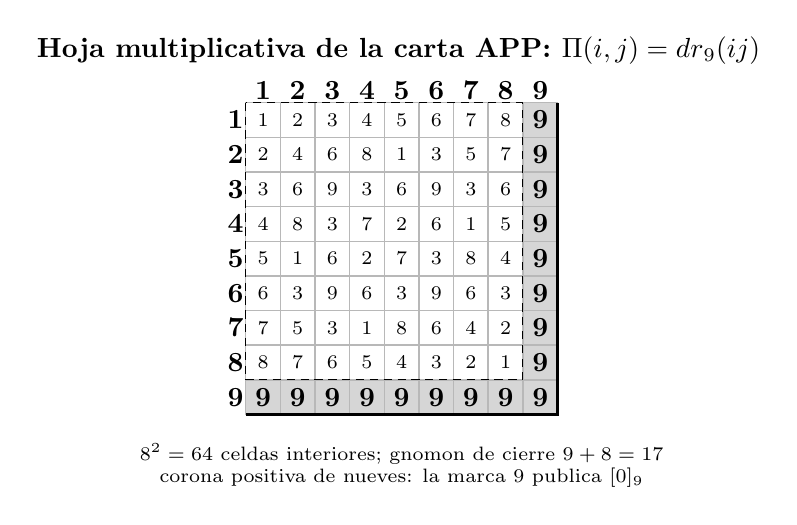
\begin{tikzpicture}[
  font=\scriptsize,
  cell/.style={minimum width=4.35mm,minimum height=4.35mm,
    inner sep=0pt,draw=black!28}]
  \node[font=\bfseries] at (1.72,.88)
    {Hoja multiplicativa de la carta APP: $\Pi(i,j)=\operatorname{dr}_9(ij)$};
  \foreach \i in {1,...,9}{
    \node[font=\bfseries] at (-.35,{-(\i-1)*.44}) {\i};
    \foreach \j in {1,...,9}{
      \pgfmathtruncatemacro{\v}{mod(\i*\j-1,9)+1}
      \pgfmathtruncatemacro{\border}{(\i==9)||(\j==9)}
      \ifnum\border=1
        \node[cell,fill=black!16,font=\bfseries]
          at ({(\j-1)*.44},{-(\i-1)*.44}) {\v};
      \else
        \node[cell,fill=white]
          at ({(\j-1)*.44},{-(\i-1)*.44}) {\v};
      \fi
    }
  }
  \foreach \j in {1,...,9}{
    \node[font=\bfseries] at ({(\j-1)*.44},.38) {\j};
  }
  \draw[very thick] (3.74,.22)--(3.74,-3.74)--(-.22,-3.74);
  \draw[densely dashed] (-.22,.22) rectangle (3.30,-3.30);
  \node[align=center,anchor=north,font=\scriptsize] at (1.76,-3.98)
    {$8^2=64$ celdas interiores; gnomon de cierre
     $9+8=17$\\corona positiva de nueves: la marca $9$ publica $[0]_9$};
\end{tikzpicture}}
\end{minipage}\hfill
\begin{minipage}[t]{.44\textwidth}
\centering
\resizebox{.98\linewidth}{!}{%
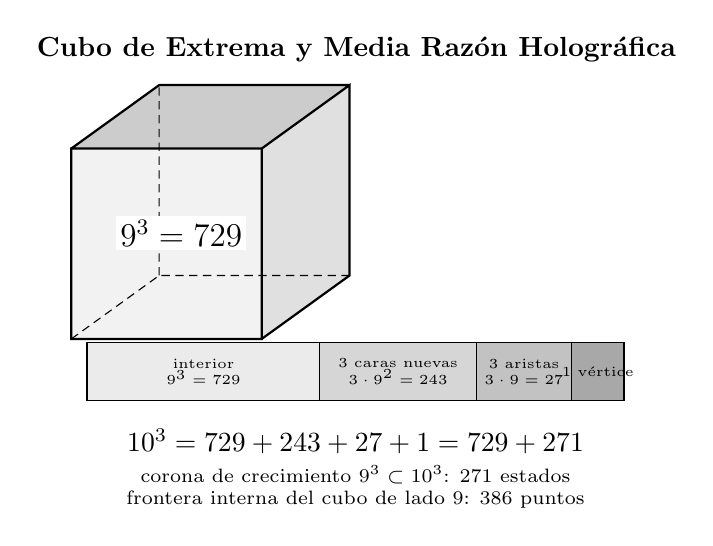
\begin{tikzpicture}[font=\scriptsize]
  \begin{scope}[x={(.78cm,0cm)},y={(.36cm,.26cm)},z={(0cm,.78cm)}]
    \coordinate (O) at (0,0,0);
    \coordinate (X) at (3.1,0,0);
    \coordinate (Y) at (0,3.1,0);
    \coordinate (XY) at (3.1,3.1,0);
    \coordinate (Z) at (0,0,3.1);
    \coordinate (XZ) at (3.1,0,3.1);
    \coordinate (YZ) at (0,3.1,3.1);
    \coordinate (XYZ) at (3.1,3.1,3.1);
    \path[fill=black!5] (O)--(X)--(XZ)--(Z)--cycle;
    \path[fill=black!12] (X)--(XY)--(XYZ)--(XZ)--cycle;
    \path[fill=black!20] (Z)--(XZ)--(XYZ)--(YZ)--cycle;
    \draw[densely dashed] (O)--(Y)--(XY) (Y)--(YZ);
    \draw[thick] (O)--(X)--(XZ)--(Z)--cycle
      (X)--(XY)--(XYZ)--(XZ) (Z)--(YZ)--(XYZ);
    \node[font=\bfseries\large,fill=white,inner sep=1.5pt]
      at (1.55,.52,1.55) {$9^3=729$};
  \end{scope}
  \node[font=\bfseries] at (3.62,3.68) {Cubo de Extrema y Media Razón Holográfica};
  \draw[fill=black!8] (0.2,-.78) rectangle (3.15,-.05);
  \node[align=center,font=\tiny] at (1.68,-.415)
    {interior\\$9^3=729$};
  \draw[fill=black!16] (3.15,-.78) rectangle (5.15,-.05);
  \node[align=center,font=\tiny] at (4.15,-.415)
    {$3$ caras nuevas\\$3\cdot9^2=243$};
  \draw[fill=black!24] (5.15,-.78) rectangle (6.35,-.05);
  \node[align=center,font=\tiny] at (5.75,-.415)
    {$3$ aristas\\$3\cdot9=27$};
  \draw[fill=black!34] (6.35,-.78) rectangle (7.02,-.05);
  \node[align=center,font=\tiny] at (6.685,-.415)
    {$1$ vértice};
  \node[font=\bfseries] at (3.61,-1.30)
    {$10^3=729+243+27+1=729+271$};
  \node[align=center] at (3.61,-1.88)
    {corona de crecimiento $9^3\subset10^3$: $271$ estados\\
     frontera interna del cubo de lado $9$: $386$ puntos};
\end{tikzpicture}}
\end{minipage}
\caption{Dos publicaciones finitas del soporte. Izquierda: la tabla de
producto con raíz digital positiva y su gnomon de cierre. Derecha: la
completación cúbica EMRH, que distingue interior, caras, aristas y vértice.
La corona de crecimiento $271$ y la frontera interna $386$ son dos
recuentos tipados: el primero mide la ampliación $9^3\subset10^3$ y el
segundo la frontera del cubo de lado $9$.}
\label{fig:app-emrh-mini}
\end{figure}

El volumen interior, las caras, las aristas y el cierre puntual quedan así
tipados como capas distintas de una misma unidad completada. Sobre las 81
celdas de la carta positiva actúan las evaluaciones
\[
\Sigma,\Pi:\mathcal D_9^2\longrightarrow\mathcal D_9,
\qquad
\Sigma(i,j)=\operatorname{dr}_9(i+j),
\qquad
\Pi(i,j)=\operatorname{dr}_9(ij),
\]
Sus residuos y cocientes levantados se definen por
\[
\begin{aligned}
R^+(i,j)&:=\Sigma(i,j),&
Q^+(i,j)&:=\frac{i+j-R^+(i,j)}9,\\
R^\times(i,j)&:=\Pi(i,j),&
Q^\times(i,j)&:=\frac{ij-R^\times(i,j)}9,
\end{aligned}
\]
y, por tanto,
\[
\begin{aligned}
\widehat\Sigma(i,j)&:=\bigl(R^+(i,j),Q^+(i,j)\bigr),\\
\widehat\Pi(i,j)&:=\bigl(R^\times(i,j),Q^\times(i,j)\bigr),
\end{aligned}
\qquad
\widehat\Sigma,\widehat\Pi:
\mathcal D_9^2\longrightarrow\mathcal D_9\times\mathbb Z_{\geq0}.
\]
La biyección \(\lambda_9^{\times2}:\mathcal D_9^2\to X_9\) transporta
estas operaciones y sus levantamientos al toro. Por tanto, APP es la tupla
\begin{equation}
\APP=\bigl(\mathcal D_9,\lambda_9,X_9,\Gamma_{\rm APP},
\operatorname{Path}(\Gamma_{\rm APP}),
\Sigma,\Pi,\widehat\Sigma,\widehat\Pi\bigr),
\label{p12-83-c3-s1:eq:app-full-definition-public}
\end{equation}
La tabla constituye una representación bidimensional de esta tupla
completa. La hoja aditiva es latina; la multiplicativa conserva
el radical ternario del anillo \(\mathbb Z/9\mathbb Z\)
\begin{equation}
R_9:=\mathbb Z/9\mathbb Z,
\qquad
\mathfrak m:=([3]_9)=\{[0]_9,[3]_9,[6]_9\}\triangleleft R_9,
\qquad \mathfrak m^2=(0).
\label{p12-83-c3-s1:eq:app-radical-369}
\end{equation}
La rotación interna es el automorfismo
\[
\rho:\mathfrak m^3\longrightarrow\mathfrak m^3,
\qquad \rho(x_1,x_2,x_3)=(x_2,x_3,x_1),
\]
cuya órbita distinguida es
\[
([3]_9,[6]_9,[0]_9)\xrightarrow{\rho}
([6]_9,[0]_9,[3]_9)\xrightarrow{\rho}
([0]_9,[3]_9,[6]_9)\xrightarrow{\rho}
([3]_9,[6]_9,[0]_9).
\]
La reducción directa envía \(3,6,9\) a \(0,0,0\). La coordenada interna
del ideal conserva, en cambio, el factor extraído:
\begin{equation}
\eta_{\mathfrak m}:(\mathfrak m,+)
\xrightarrow{\;\sim\;}(\mathbb Z/3\mathbb Z,+),
\qquad
\eta_{\mathfrak m}([3a]_9):=[a]_3,
\qquad
([3]_9,[6]_9,[0]_9)
\xmapsto{\;\eta_{\mathfrak m}^{\times3}\;}
([1]_3,[2]_3,[0]_3),
\label{p12-83-c3-s1:eq:app-369-120}
\end{equation}
de modo que el sector \(3,6,9\) permanece íntegro y su coordenada interna se
lee como \(1,2,0\). Esta aplicación pertenece al radical de APP; la
proyección temporal de TRIT constituye el lector calendárico posterior. Las
tres clases calendáricas
quedan separadas como
\[
\mathcal C_+=\{1,4,7\},\qquad
\mathcal C_-=\{2,5,8\},\qquad
\mathcal C_0=\{3,6,9\}.
\]
La incompatibilidad entre ambas hojas se vuelve un invariante medible. Sobre
\(\mathscr A_3=\mathcal D_9^3\), con medida uniforme
\(\nu_3(x)=9^{-3}\), sea
\(\mathcal H_3=L^2(\mathscr A_3,\nu_3)\). Definimos
\[
\Sigma_3,\Pi_3:\mathscr A_3\longrightarrow\mathcal D_9,
\qquad
\Sigma_3(x)=\operatorname{dr}_9(x_1+x_2+x_3),
\qquad
\Pi_3(x)=\operatorname{dr}_9(x_1x_2x_3),
\]
y los proyectores ortogonales
\[
P_{\Sigma,3}:=\mathbb E_{\nu_3}[\,\cdot\mid\sigma(\Sigma_3)],
\qquad
P_{\Pi,3}:=\mathbb E_{\nu_3}[\,\cdot\mid\sigma(\Pi_3)]
\in\mathcal B(\mathcal H_3).
\]
La enumeración conjunta de las \(9^3\) palabras determina entonces
\[
\bigl\|[P_{\Sigma,3},P_{\Pi,3}]\bigr\|=\frac{\sqrt3}{4},
\qquad
B_c=7I+2R=9P_++5P_-,
\qquad
459-405=54.
\]
El primer número reaparece como prefactor electrónico; el segundo organiza
el bloque central; el tercero registra el defecto global suma--producto.

\subsection{TRIT: unidad local topológica y unidad de relación temporal}

HMT fija primero la firma visible
\begin{equation}
\mathrm{TRIT}_{\rm vis}=\{-1,0,+1\},
\qquad \tau\in\mathrm{TRIT}_{\rm vis}.
\label{p12-83-c3-s1:eq:trit-visible-signature}
\end{equation}
Frente a la unidad binaria, el TRIT conserva tres regímenes locales. En la
distribución uniforme, su información y su entropía se distinguen como
\begin{equation}
I_{\rm TRIT}=\log3\ \text{nats}=\log_2 3\ \text{bits},
\qquad S_{\rm TRIT}=k_BI_{\rm TRIT}.
\label{p12-83-c3-s1:eq:trit-information-unit}
\end{equation}
El bit sigue siendo la unidad binaria; el TRIT es la unidad mínima capaz de
distinguir simultáneamente retorno, umbral y apertura. La igualdad
\eqref{p12-83-c3-s1:eq:trit-information-unit} cuantifica la información de la terna; el
coste \(k_B\Theta\log3\) pertenece al lector térmico de reinicio posterior.
Mecánica Dimensional conserva además el antecedente aritmético de esa firma.
Para \((i,j)\in\mathcal D_9^2\), la celda aritmética levantada asociada es
\begin{equation}
c_{\rm MD}(i,j;\tau)=
\bigl(i,j;R^+,Q^+,R^\times,Q^\times;\tau\bigr).
\label{p12-83-c3-s1:eq:trit-complete-local-unit}
\end{equation}
Los residuos \(R^+,R^\times\) son la publicación visible de las dos hojas;
los cocientes \(Q^+,Q^\times\) conservan la memoria exacta de la división
euclídea; y \(\tau\) orienta la transición. La firma visible ocupa el primer
nivel; la celda que la porta añade los antecedentes aritméticos, y el estado
enriquecido completa después frontera, ruta, fase y supervivencia.

Conviene separar cuatro estratos. La firma visible es \(\tau\); el par
residuo--acarreo es su levantamiento local; \(c_{\rm MD}\) es la celda
aritmética de APP provista de esa firma; y el estado TPK añade extensión,
frontera, registro genealógico, fase y supervivencia. Esta jerarquía conserva la identidad
propia de la coordenada observada, su levantamiento, la celda portadora y la
historia enriquecida que la transporta.

En la carta ternaria balanceada, el entero local levantado
\(n\in\{-4,-3,\ldots,3,4\}\) se descompone de manera única como
\begin{equation}
\widehat n=(r,\kappa),
\qquad n=r+3\kappa,
\qquad r,\kappa\in\{-1,0,+1\}.
\label{p12-83-c3-s1:eq:trit-balanced-lift}
\end{equation}
La firma visible es \(\tau=r\); \(\kappa\) conserva el carry que la proyección
\(n\mapsto r\) olvidaría.
La fibra sobre el cero visible contiene tres estados distintos,
\[
0^+=(0,+1),\qquad 0^0=(0,0),\qquad 0^-=(0,-1),
\]
porque \(n=-3,0,3\) poseen el mismo residuo visible y carries distintos. Éste
es el levantamiento topológico mínimo de MD: una transición orientada de APP
queda provista de la información necesaria para invertirla y para decidir qué
prolongaciones siguen siendo compatibles.

La firma posee además una regla de memoria de hoja. Si \(m_k\) es el modo
aritmético activo, entonces
\begin{equation}
m_{k+1}=
\begin{cases}
\Sigma,&\tau_k=+1,\\
\Pi,&\tau_k=-1,\\
m_k,&\tau_k=0.
\end{cases}
\label{p12-83-c3-s1:eq:trit-zero-memory}
\end{equation}
El cero codifica retención de la hoja anterior. Por eso la palabra
\((+1,-1,0)\) publica la secuencia \((\Sigma,\Pi,\Pi)\): el tercer estado
conserva el modo multiplicativo activo.

La relación temporal se obtiene al parametrizar ordenadamente estas celdas.
Cada firma porta un álgebra cuadrática
\begin{equation}
\mathbb A_\tau=\mathbb R[X]/(X^2+\tau),
\qquad J_\tau=[X],
\label{p12-83-c3-s1:eq:trit-quadratic-algebra-local}
\end{equation}
de modo que
\[
\begin{array}{c@{\qquad}c@{\qquad}l}
\toprule
\tau & J_\tau^2 & \text{relación temporal ordenada}\\
\midrule
+1 & -I & \text{retorno elíptico, memoria y pasado},\\
0  & 0  & \text{umbral parabólico y presente},\\
-1 & +I & \text{apertura hiperbólica bidireccional y futuro}.\\
\bottomrule
\end{array}
\]
El TRIT precede al tiempo exterior: primero clasifica el tipo algebraico y
topológico del transporte; después, una parametrización ordenada lo publica
como relación temporal. La doble dirección queda tipada por la involución
exacta
\begin{equation}
\mathcal C_{\rm rev}(\tau_1,\ldots,\tau_n)
=(-\tau_n,\ldots,-\tau_1),
\qquad \mathcal C_{\rm rev}^2=I,
\label{p12-83-c3-s1:eq:trit-time-reversal}
\end{equation}
que intercambia retorno y apertura y conserva el umbral. En la hoja
hiperbólica, \(P_\pm=(I\pm J_{-1})/2\) separan las dos direcciones propias y
la reversión intercambia sus orientaciones. Topología y tiempo son, así, las
dos lecturas coordinadas del TRIT.

La involución combinatoria \(\mathcal C_{\rm rev}\) y una conjugación
operatorial \(C\) pertenecen, sin embargo, a dominios distintos. En una
realización dinámica separada, provista de \(H=H^*\),
\(CJ_EC^{-1}=-J_E\) y \(CHC^{-1}=H\), fijamos una escala de acción interna
\(\hbar_{\rm int}>0\) y escribimos
\(h_{\rm int}:=2\pi\hbar_{\rm int}\). Entonces
\begin{equation}
U(t)=\exp(-J_EHt/\hbar_{\rm int}),
\qquad CU(t)C^{-1}=U(-t).
\label{p12-83-c3-s1:eq:trit-bidirectional-propagator}
\end{equation}
El entrelazador que transporta palabras TRIT a la realización dinámica fija
la correspondencia entre \(\mathcal C_{\rm rev}\) y \(C\). La doble
orientación local proporciona el dominio de esa construcción.

\subsection{TPK: categoría de transporte y evolución de fase}

El \emph{Topological Phase Kernel} es la categoría de transporte sobre la
base observable de APP que compone cifras, palabras, operadores y relaciones
de prolongación en un mismo estado enriquecido. Su arquitectura interna se distribuye en
ocho clases operatorias, diferenciadas por dominio, codominio y función:
\begin{enumerate}[label=\textup{(\roman*)},leftmargin=2.25em]
\item soporte observable y estado enriquecido;
\item selector interno de hoja \(M_{\rm ph}:\{1,\ldots,9\}\to\{+1,-1,0\}\);
\item traslaciones cardinales y evolución visible \(F_{\rm obs}\);
\item lectores y cocientes nonádico, trítico y de bloque \(1000\);
\item memoria, acarreo, cilindro, frontera y registro genealógico;
\item periodicidad y retorno
\(C_{12}\hookrightarrow C_{108}\twoheadrightarrow C_9\),
\(\mathcal K_{27}\) y canales \(90/120\);
\item prolongaciones \(\operatorname{Ext}_r\), cilindros, supervivencia y
extensión natural bidireccional;
\item funtores de salida arquimediana, excepcional calibrada y dimensional.
\end{enumerate}
El retorno de 27 pasos es el morfismo compuesto
\begin{equation}
\mathcal K_{27}:=F_{\rm obs}^{27},
\qquad \mathcal K_{27}^{4}=F_{\rm obs}^{108}.
\label{p12-83-c3-s1:eq:tpk-kernel-27}
\end{equation}
Su cuarto iterado restaura la fase observable del calendario, mientras la
memoria y el estado TPK completo continúan su trayectoria;
\(\mathcal K_{27}\) es el morfismo de retorno interno de \(C_{108}\).
El calendario \(C_{108}\), la conexión nonádica, la extensión bilateral y
los lectores ocupan lugares tipados dentro de esta arquitectura. Sea
\(\mathsf P_{\rm APP}\) la categoría
libre del grafo dirigido de APP y
\(\mathsf P_{\rm APP}^{(2)}=\mathsf P_{\rm APP}\times
\mathsf P_{\rm APP}\) su lectura simultánea suma--producto. Sea además
\[
\mathcal Q_{\rm obs}
=X_9^2\times\{N,E,S,O\}^2\times\Theta_{108},
\qquad \Theta_{108}=\mathbb Z/108\mathbb Z,
\]
donde, para el representante
\(\widetilde\theta\in\{0,\ldots,107\}\),
\[
r(\theta)=1+(\widetilde\theta\bmod9),
\qquad g_0(\theta)=[\widetilde\theta]_9,
\]
\[
\tau(\theta)=
\begin{cases}
+1,&r(\theta)\in\{1,4,7\},\\
-1,&r(\theta)\in\{2,5,8\},\\
0,&r(\theta)\in\{3,6,9\},
\end{cases}
\qquad
\mu(\theta)=
\begin{cases}
\Sigma,&\tau(\theta)=+1,\\
\Pi,&\tau(\theta)=-1,\\
\varnothing,&\tau(\theta)=0.
\end{cases}
\]
La etiqueta calendárica \(\mu=\varnothing\) señala el umbral, y la memoria
dinámica \(m_k\) de \eqref{p12-83-c3-s1:eq:trit-zero-memory} retiene la última hoja
activa. Una configuración
\(q=(p^\Sigma,p^\Pi,d^\Sigma,d^\Pi,\theta)\) conserva las dos posiciones,
las dos direcciones cardinales y el índice de calendario. La evolución
visible \(F_{\rm obs}\) activa la hoja indicada por TRIT, transporta la
posición correspondiente y avanza \(\theta\). Denotemos por
\(\mathsf P_{\rm obs}\) la categoría libre generada por las flechas
\(q\to F_{\rm obs}(q)\). Cada flecha induce un par de caminos de APP y
define el funtor de base
\begin{equation}
B:\mathsf P_{\rm obs}\longrightarrow\mathsf P_{\rm APP}^{(2)}.
\label{p12-83-c3-s1:eq:tpk-bivariant-base-functor}
\end{equation}

Sobre cada \(q\) se dispone la fibra tipada
\begin{equation}
\mathcal F_q=
\mathsf O_q\times\mathsf H_q\times\mathsf C_q\times\mathsf S_q
\times\mathsf B_q\times\mathsf\Lambda_q,
\label{p12-83-c3-s1:eq:tpk-fiber}
\end{equation}
Sus seis factores conservan, respectivamente, orientación y hoja; residuo y
cociente; acarreo; firma; cilindro y frontera; y registro ordenado de
transporte. Memoria y supervivencia son propiedades de la composición y de
las relaciones de prolongación.

Para una ruta \(r:q\to q'\), la relación
\begin{equation}
\operatorname{Ext}_r\subseteq\mathcal F_q\times\mathcal F_{q'}
\label{p12-83-c3-s1:eq:tpk-extension-relation}
\end{equation}
contiene todas las continuaciones admisibles y satisface
\[
\Delta_q\subseteq\operatorname{Ext}_{\operatorname{id}_q},
\qquad
\operatorname{Ext}_{r_2}\circ\operatorname{Ext}_{r_1}
\subseteq\operatorname{Ext}_{r_2\circ r_1}.
\]
Los transportes respetan identidades y composición:
\begin{equation}
\begin{gathered}
\mathsf H(\operatorname{id}_q)=I,
\quad \mathsf C(\operatorname{id}_q)=I,
\quad \mathsf\Lambda(\operatorname{id}_q)=I,
\quad \kappa(\operatorname{id}_q)=0,\\
\mathsf H(r_2\!\circ r_1)=\mathsf H(r_2)\mathsf H(r_1),
\quad
\mathsf C(r_2\!\circ r_1)=\mathsf C(r_2)\mathsf C(r_1),
\quad
\mathsf\Lambda(r_2\!\circ r_1)=
\mathsf\Lambda(r_2)\mathsf\Lambda(r_1).
\end{gathered}
\label{p12-83-c3-s1:eq:tpk-functorial-transport}
\end{equation}
Junto con estas leyes functoriales, las coordenadas transportadas obedecen
\begin{equation}
\begin{aligned}
h'&=\mathsf H(r)(h),\\
c'&=\mathsf C(r)(c)+\kappa(r),\\
\lambda'&=\mathsf\Lambda(r)(\lambda),\\
\sigma'&=\operatorname{Sig}_{q'}(h',c',\lambda'),
\end{aligned}
\qquad
\kappa(r_2\circ r_1)
=\kappa(r_2)+\mathsf C(r_2)\kappa(r_1).
\label{p12-83-c3-s1:eq:tpk-typed-transport}
\end{equation}
La última identidad es el cociclo de acarreo que hace asociativa la
composición con memoria.

El TPK es entonces la categoría \(\mathsf{TPK}\) cuyos objetos son
\begin{equation}
x=(q,o,h,c,\sigma,C,b,\lambda),
\qquad (o,h,c,\sigma,(C,b),\lambda)\in\mathcal F_q,
\label{p12-83-c3-s1:eq:tpk-enriched-object}
\end{equation}
y cuyos morfismos \(x\to x'\) son las ternas \((r,x,x')\) tales que
las coordenadas satisfacen \eqref{p12-83-c3-s1:eq:tpk-typed-transport} y
\((f_x,f_{x'})\in\operatorname{Ext}_r\), donde
\(f_x\in\mathcal F_q\) y \(f_{x'}\in\mathcal F_{q'}\). La composición es
\begin{equation}
(r_2,x',x'')\circ(r_1,x,x')
=(r_2\circ r_1,x,x''),
\label{p12-83-c3-s1:eq:tpk-morphism-composition}
\end{equation}
\Needspace{7\baselineskip}
la identidad es \((\operatorname{id}_q,x,x)\), y el funtor
\begin{equation}
p:\mathsf{TPK}\longrightarrow\mathsf P_{\rm obs},
\qquad p(x)=q,
\qquad p(r,x,x')=r,
\label{p12-83-c3-s1:eq:tpk-base-functor}
\end{equation}
publica la configuración visible sin identificar estados de la misma fibra.
La definición fija una categoría sobre una base; no presupone que sea una
fibración categórica ni que toda flecha admita un levantamiento cartesiano.
Las proyecciones locales quedan separadas por tipo:
\[
\pi_{\rm TRIT}:\operatorname{Ob}(\mathsf{TPK})
\longrightarrow\mathrm{TRIT}_{\rm vis},
\qquad
\pi_{\rm TRIT}(x)=\tau(\theta),
\]
\[
\pi_{\rm loc}(x)=
\bigl(\pi_{\rm TRIT}(x),\mu(\theta),o,h,c,
\sigma,\lambda,g_0(\theta)\bigr).
\]
La primera recupera únicamente la firma TRIT visible. La segunda conserva
además la etiqueta calendárica de hoja, la orientación, el par
residuo--cociente, el acarreo, la firma de transporte, el registro genealógico y la fase,
pero todavía olvida el cilindro, su etiqueta de borde y otras coordenadas de
\(q\). Ésta es la razón por la que ni el TRIT visible ni su registro local
sustituyen al estado enriquecido del TPK.

El nombre recoge tres funciones inseparables. \emph{Topological} remite a
la categoría de caminos, la incidencia, el borde y la prolongación por
cilindros; \emph{Phase} remite al índice nonádico, al calendario orientado y
a la holonomía; \emph{Kernel} nombra el núcleo persistente de transporte que
permanece antes de contraer el estado mediante un lector. Formalmente, el
objeto es la categoría anterior: una topología adicional sobre objetos o
morfismos, o su identificación con el núcleo lineal de un mapa, requiere
datos independientes.

En consecuencia, dos rutas con el mismo extremo visible pueden seguir siendo
objetos distintos por hoja, cociente, acarreo, frontera, cilindro, fase o
registro. El TPK no elige una salida escalar: conserva el antecedente común
del que parten las publicaciones arquimediana, excepcional y dimensional.

% Estas consecuencias se publican después de la construcción correlativa y
% del paso al límite de los capítulos 4 y 5. Se definen aquí para preservar
% íntegramente su procedencia, pero no se ejecutan antes de que exista el
% continuo al que se aplican.
\long\def\HMTDeferredContinuumConsequences{%
\section{Consecuencias y publicaciones del continuo construido}

\subsection{Teorema de ensamblaje terminal de las construcciones correlativas generadas por el estado común}

Cada profundidad \(k\) posee un estado enriquecido \(\mathcal E_k\) con
todas sus emisiones supervivientes y un único constructor correlativo
\begin{equation}
\mathcal O_k:\mathcal E_k\longrightarrow\mathcal Z_k,
\qquad
\widehat x_k\longmapsto
\mathcal O\bigl(\{\mathfrak e_\alpha:
\alpha\in\operatorname{Ch}_k(\widehat x_k)\}\bigr).
\label{p12-83-c3-s1:eq:five-features-single-constructor}
\end{equation}
El valor de \(\mathcal O_k\) conserva simultáneamente las coordenadas
espectral, solenoidal, gauge, coherente y determinantal,
\begin{equation}
(\mathrm{sp},\mathrm{sol},\mathrm{gau},\mathrm{coh},\mathrm{det}),
\label{p12-83-c3-s1:eq:five-features-coordinates}
\end{equation}
como cinco características del mismo estado y del mismo registro genealógico. Los
truncamientos
\[
u^{\mathfrak e}_{\ell,k}:\mathcal E_\ell\to\mathcal E_k,
\qquad
u^{\mathcal O}_{\ell,k}:\mathcal Z_\ell\to\mathcal Z_k
\]
satisfacen la naturalidad única
\begin{equation}
u^{\mathcal O}_{\ell,k}\circ\mathcal O_\ell
=\mathcal O_k\circ u^{\mathfrak e}_{\ell,k},
\qquad \ell\ge k.
\label{p12-83-c3-s1:eq:five-features-naturality}
\end{equation}
Por ello, la acción correlativa pasa al límite como
\begin{equation}
\mathcal O_\infty:
\mathcal C_{\rm cont}^{\rm disc}:=\varprojlim_k\mathcal E_k
\longrightarrow
\mathcal Z_\infty:=\varprojlim_k\mathcal Z_k.
\label{p12-83-c3-s1:eq:five-features-infinite-operator}
\end{equation}
Las cinco aplicaciones terminales son vistas intrínsecas de ese único valor:
\begin{equation}
\boxed{
\mathfrak G_T^{\rm int}:=
\operatorname{View}_T\!\left(
\mathcal O_\infty(\mathcal C_{\rm cont}^{\rm disc})\right),
\quad
T\in\{\mathrm{sp},\mathrm{sol},\mathrm{gau},
\mathrm{coh},\mathrm{det}\}.}
\label{p12-83-c3-s1:eq:five-features-views}
\end{equation}
La simultaneidad precede a las resoluciones especializadas: cada vista expone
la coordenada requerida y el estado completo conserva las otras cuatro.

\subsection{Supervivencia y límite inverso}

Sea \(\operatorname{Surv}^{(\chi)}_N\) el conjunto de historias de
profundidad \(N\) que satisfacen simultáneamente las leyes activas del canal
\(\chi\) y admiten prolongación. Definimos las truncaciones compatibles
\[
\tau_{N+1,N}:\operatorname{Surv}^{(\chi)}_{N+1}
\longrightarrow\operatorname{Surv}^{(\chi)}_N
\]
Estas conservan el prefijo enriquecido. El continuo genealógico es el límite
\begin{equation}
X_\chi=\varprojlim_N
\bigl(\operatorname{Surv}^{(\chi)}_N,\tau_{N+1,N}\bigr),
\qquad
\tau_{N+1,N}(x_{N+1})=x_N.
\label{p12-83-c3-s1:eq:inverse-survival}
\end{equation}
El espacio global de secciones supervivientes y una de sus secciones
enriquecidas se denotan, respectivamente, por
\begin{equation}
X_\infty:=\bigsqcup_\chi X_\chi,
\qquad
\widehat\Omega_\infty\in X_\infty.
\label{p12-83-c3-s1:eq:global-survival-space}
\end{equation}
El lector arquimediano global es
\begin{equation}
P_{\rm arq}:=\operatorname{ev}_{\mathbb R}:
X_\infty\longrightarrow\mathbb R;
\label{p12-83-c3-s1:eq:archimedean-reader}
\end{equation}
su restricción a cada canal evalúa la intersección unitaria de los cilindros
compatibles de la sección correspondiente.
Cuando interviene el lector excepcional, \(X_\infty^{\rm cal}\subseteq
X_\infty\) denota el subespacio en el que se ha fijado el tipo de calibración
de \eqref{p12-83-c3-s1:eq:exceptional-calibration}.
La supervivencia determina la sección por compatibilidad interna: cada
historia debe ser prolongable en el sistema completo. El lector numérico
interviene después para certificar y publicar la intersección del
descendiente ya compatible.

\subsection{Conexión nonádica conjunta, holonomía y memoria vertical}

En profundidad \(K\), la holonomía del retorno nonádico es inicialmente la
correspondencia tipada
\begin{equation}
\Gamma_{9,K}=\operatorname{Hol}_{C_9}(\nabla_{\rm TPK}):
\widehat{\mathcal X}_K\rightrightarrows
\widehat{\mathcal X}_{K+9}.
\label{p12-83-c3-s1:eq:gamma9}
\end{equation}
Sus iterados son composiciones relacionales. Sólo cuando cada estado posee
una prolongación compatible única se restringe a un mapa, y sólo cuando ese
mapa es invertible constituye una monodromía. Esta distinción conserva todas
las extensiones supervivientes antes de seleccionar una sección.
Tras nueve fases retorna la fase local, mientras el estado completo avanza:
\[
g(K+9)=g(K),\qquad q_{{\rm mem},K+9}=q_{{\rm mem},K}+1,
\qquad \widehat x_{K+9}\ne\widehat x_K\ \text{en general}.
\]
Bloque, cilindro, prefijo, acarreo y memoria continúan evolucionando. Ésta
es la diferencia entre periodicidad visible y retorno con biografía.

El estado transportado en el nivel (K) puede exhibirse como
\begin{equation}
\widehat x_K=
(B_K,C_K,p_K,c_K,\Sigma_K,W_K,g(K),q_{{\rm mem},K},s_K),
\label{p12-83-c3-s1:eq:enriched-state-k}
\end{equation}
donde cada coordenada tiene una ley de transporte propia. El retorno de fase
se representa sobre el catálogo
\[
\mathcal U_6^{\rm cat}\cong\mathfrak S_+\times\mathfrak S_\times,
\qquad |\mathfrak S_+|=18,
\qquad |\mathfrak S_\times|=26.
\]
Los promedios condicionales
\[
(E_+f)(s,e)=\frac1{18}\sum_{s'\in\mathfrak S_+}f(s',e),
\qquad
(E_\times f)(s,e)=\frac1{26}\sum_{e'\in\mathfrak S_\times}f(s,e')
\]
conmutan. La palabra de fase
\(\tau=(+1,-1,0,+1,-1,0,+1,-1,0)\) aplica
\(E_+,E_\times,I\) en ese orden, y una vuelta se cierra mediante
\begin{equation}
\mathcal K_{\rm ph}^{\,9}
=(E_+E_\times)\otimes I_{\ell^2(C_9)},
\qquad
\bigl\langle\delta_u,E_+E_\times\delta_v\bigr\rangle
=\frac1{468}\quad(u,v\in\mathcal U_6^{\rm cat}).
\label{p12-83-c3-s1:eq:joint-nine-holonomy}
\end{equation}
Las hojas suma y producto no actúan como filtros independientes: son dos
componentes de una única holonomía que sólo se cierra después de recorrer el
ciclo completo.

La coligación compresión--expresión separa lo que vuelve y lo que permanece
como memoria. Si (J) incrusta el espacio de historias en el espacio de
fase, (T) es la compresión superviviente y \(\eta\) el canal de defecto,
entonces
\begin{equation}
\boxed{
U_{\Gamma_9}J=JT+\eta,
\qquad J^*\eta=0,
\qquad I-T^*T=\eta^*\eta.}
\label{p12-83-c3-s1:eq:compression-expression}
\end{equation}
La primera igualdad descompone el transporte en retorno comprimido y
expresión de memoria; la segunda prueba su ortogonalidad; la tercera mide
exactamente la información que no cabe en la sombra periódica. Así queda
formalizada la afirmación central: vuelve la fase, no el estado completo.

La memoria vertical se organiza mediante la extensión cíclica orientada
\begin{equation}
0\longrightarrow C_{12}\xrightarrow{\,\iota\,}C_{108}
\xrightarrow{\,p\,}C_9\longrightarrow0,
\qquad
c(r,r')=\left[\left\lfloor\frac{r+r'}9\right\rfloor\right]_{12}.
\label{p12-83-c3-s1:eq:c108-extension}
\end{equation}
Aquí \(\iota([b]_{12})=[9b]_{108}\) y
\(p([\theta]_{108})=[\theta]_9\). La extensión no se escinde:
\(C_{108}\) tiene exponente 108, mientras
\(C_{12}\times C_9\) tiene exponente 36.
El cociclo registra el acarreo de cada vuelta de la base \(C_9\) en la
memoria dodecafásica \(C_{12}\). \(C_{108}\) es, por tanto, un calendario
orientado de fase y memoria. Sólo después de la carta dimensional esa
extensión se realiza como reloj cuántico finito de 108 pasos.

El levantamiento local de MD que porta la firma TRIT es la unidad
topológico--temporal de ese cristal genealógico.
Sobre
\(\mathcal H_{\rm clk}=\mathbb C^{108}\), con base
\(\{|j\rangle:j\in\mathbb Z/108\mathbb Z\}\), sean
\[
\zeta=e^{2\pi\ii/108},\qquad
|\widetilde k\rangle=\frac1{\sqrt{108}}
\sum_{j=0}^{107}\zeta^{jk}|j\rangle,
\qquad U_{\rm clk}|j\rangle=|j+1\rangle.
\]
\Needspace{12\baselineskip}
Con \(\omega_0=2\pi/(108t_0)\), el Hamiltoniano
\begin{equation}
H_{\rm clk}=\hbar_{\rm int}\omega_0
\sum_{k=0}^{107}k\,|\widetilde k\rangle\langle\widetilde k|
\label{p12-83-c3-s1:eq:trit-time-crystal-hamiltonian}
\end{equation}
genera exactamente
\begin{equation}
U_{\rm step}=\exp\!\left(
-\frac{\ii H_{\rm clk}t_0}{\hbar_{\rm int}}\right)=U_{\rm clk},
\qquad U_{\rm step}^{108}=I,
\label{p12-83-c3-s1:eq:trit-time-crystal-period}
\end{equation}
Si \(Z_{\rm clk}|j\rangle=\zeta^j|j\rangle\), entonces
\begin{equation}
\langle j_0|U_{\rm step}^{-n}Z_{\rm clk}U_{\rm step}^{n}|j_0\rangle
=\zeta^{j_0+n},
\label{p12-83-c3-s1:eq:trit-time-crystal-observable}
\end{equation}
cuya órbita posee periodo primitivo 108. En el vocabulario HMT, éste es el
cristal temporal genealógico interno: el calendario observable cierra,
\(C_{12}\) registra la vuelta y el estado TPK enriquecido no tiene por qué
retornar. La realización ulterior como fase física macroscópica exige,
además, protocolo de Floquet, respuesta subarmónica primitiva, robustez,
persistencia y un mecanismo de protección; esa carta no altera el teorema
finito de periodicidad unitaria.

\subsection{Publicación arquimediana, número genealógico y medición}

La publicación arquimediana utiliza cilindros ternarios semiabiertos
\begin{equation}
I_{N,L}=\left[\frac{N}{3^L},\frac{N+1}{3^L}\right),
\qquad \operatorname{diam}I_{N,L}=3^{-L}\longrightarrow0.
\label{p12-83-c3-s1:eq:ternary-cylinders}
\end{equation}
Una sección compatible determina cilindros encajados y, por completitud, un
único punto real. El número HMT es la sección misma,
\begin{equation}
x=(x_N)_N\in X_\chi
=\varprojlim_N\operatorname{Surv}^{(\chi)}_N,
\label{p12-83-c3-s1:eq:hmt-number-as-section}
\end{equation}
no la tupla formada por ella y sus evaluaciones. El valor aparece cuando un
lector olvida parte de la genealogía.
Por tanto, la precisión es profundidad: medir significa descender a un
cilindro más fino mientras el prefijo causal permanece en el antecedente.
La recta real se reconstruye como cociente arquimediano de un espacio de
historias mucho más rico.

\subsection{Realización dimensional del estado HMT: mapa de pantalla, magnitud observable y carta espectral}

La Mecánica Dimensional comienza donde el estado genealógico se acopla a una
frontera de realización. Fijado un cuerpo \(K_n\), sea \(M_n(x)\) el módulo
generado por los canales de prolongación de un estado \(x\), sea
\(\mathcal R_n(x)\) el submódulo de sus relaciones y sea \(\beta_n(x)\) el
dato de borde conservado. La pantalla dimensional es
\begin{equation}
\Sigma_n(x)=\bigl(K_n,M_n(x),\beta_n(x),\mathcal R_n(x)\bigr),
\qquad
d_{\Sigma_n}(x)=\dim_{K_n}\frac{M_n(x)}{\mathcal R_n(x)}.
\label{p12-83-c3-s1:eq:md-screen}
\end{equation}
Si \(M_n(x)\simeq K_n^{g_n}\) y las columnas de \(R_n(x)\) generan las
relaciones, entonces
\begin{equation}
\boxed{d_{\Sigma_n}(x)=g_n-\operatorname{rank}_{K_n}R_n(x).}
\label{p12-83-c3-s1:eq:md-rank}
\end{equation}
La dimensión no se adjunta como etiqueta: es el número de canales
independientes que sobreviven después de imponer las relaciones de frontera.

Una magnitud física es una sección de una recta dimensional \(L_D\); una
unidad es una carta \(\chi_u:L_D\to\mathbb R\) que publica su coordenada.
Por ello
\begin{equation}
\text{estado TPK}\longrightarrow\Sigma_n(x)
\longrightarrow s_D\in\Gamma(L_D)
\xrightarrow{\;\chi_u\;}[s_D]_u\in\mathbb R
\label{p12-83-c3-s1:eq:md-measurement-chain}
\end{equation}
separa de forma exacta estructura, tipo dimensional y número medido. Medir
consiste en acoplar una sección a un aparato reversible, imponer
compatibilidad de borde y aplicar el lector; cambiar de unidades cambia
\(\chi_u\), no la sección ni su genealogía.

\subsection{Doble proyección matemática y realización dimensional}

La rama excepcional conserva datos de calibre que la publicación real no
necesita. Sea \(\mathscr C_{\rm exc}\) el espacio de calibraciones y sea
\begin{equation}
\mathfrak E:
X_\infty^{\rm cal}\times\mathscr C_{\rm exc}
\longrightarrow\mathbf{Exc}
\label{p12-83-c3-s1:eq:exceptional-calibrated-reader}
\end{equation}
el lector de incidencia. Fijamos una vez
\begin{equation}
\begin{aligned}
\chi_{\rm exc}=\bigl(&\text{orden proyectivo},\ \text{calibre de Paley},
 \ \text{dodecada},\\
 &\text{alineamiento de incidencia},\ \text{cámara reticular}\bigr)
 \in\mathscr C_{\rm exc}
\end{aligned}
\label{p12-83-c3-s1:eq:exceptional-calibration}
\end{equation}
y abreviamos
\(\mathfrak E_{\chi_{\rm exc}}(x):=\mathfrak E(x,\chi_{\rm exc})\).
El calibre inicial se transporta por la historia; no vuelve a elegirse en
cada profundidad.

El mismo límite calibrado admite entonces dos lectores con codominios
distintos:
\begin{equation}
\mathbb R
\xleftarrow{\;\operatorname{ev}_{\mathbb R}\;}
X_\infty^{\rm cal}
\xrightarrow{\;\mathfrak E_{\chi_{\rm exc}}\;}
\mathbf{Exc}.
\label{p12-83-c3-s1:eq:double-projection}
\end{equation}
La primera rama contrae cilindros hasta un valor continuo. La segunda
conserva incidencias, orientaciones, calibre y frontera. Ambas descienden en
paralelo del mismo estado fuente. Esta bifurcación explica conjuntamente la
continuidad métrica y la emergencia de simetrías excepcionales. La segunda
rama es una reconstrucción calibrada: es exacta una vez fijado
\(\chi_{\rm exc}\), pero el estado desnudo no selecciona retrospectivamente
los cinco datos que componen ese calibre.

La realización dimensional no serializa esas dos ramas. Es un tercer lector
del mismo antecedente:
\begin{equation}
P_{\rm dim}:X_\infty\longrightarrow
\mathcal R_{\rm MD},
\qquad
\mathcal R_{\rm MD}=
\{\text{acción, masa, campo, geometría, información}\}.
\label{p12-83-c3-s1:eq:dimensional-publication}
\end{equation}
De este modo, un número, una simetría y una magnitud física pueden compartir
genealogía sin confundirse ni reducirse entre sí.

La tesis del continuo queda así formulada con precisión: la realidad
arquimediana es la sombra de radio cero de historias discretas infinitamente
refinables; aquello que la sombra omite reaparece como memoria, incidencia,
geometría y estructura física.

% RESULTADO_RECUPERADO. Owner íntegro de la dinámica del cociente, el retorno
% observable y los cociclos de modo y orientación. Se subordina a la única
% construcción APP--TRIT--TPK sin abrir un origen alternativo.
\begin{HMTScientificOwnerSubordinated}
\chapter{Extensiones supervivientes, monodromía y dinámica del cociente}
\label{chap:extensiones-dinamica-cociente}
\index{supervivencia!extensión global}
\index{monodromía!retorno nonádico}
\index{medida!catálogo de emisiones}

El lenguaje de los caminos necesita una precisión decisiva. Un camino de
APP, una emisión visible, una historia enriquecida de TPK y una sección
global no son cuatro nombres para el mismo objeto. Constituyen cuatro niveles
consecutivos de una misma construcción. El camino conserva el orden
posicional; la emisión conserva una lectura finita; la historia añade firma,
acarreo, orientación, frontera y memoria; la sección global exige que todos
sus prefijos sobrevivan simultáneamente a cualquier profundidad.

Esta jerarquía permite separar dos cuestiones que habían permanecido
entremezcladas. La primera es lógica: bajo qué hipótesis un prefijo finito
pertenece de verdad a una extensión infinita compatible. La segunda es
dinámica: qué significa transportar una sola historia y qué significa
transferir simultáneamente todas sus continuaciones compatibles. La
distinción es esencial en APP\@. Una trayectoria determinada lleva un estado a
otro; una transferencia de caminos lleva una distribución de extensiones a
otra distribución.

En esta sección se resuelve el problema finito de profundidad seis. La
cronología determinista publicada posee retorno visible y no puede seleccionar
una probabilidad única. En cambio, el transporte sesgado por la fase nonádica,
cuando cada canal activo se interpreta como la renovación normalizada de toda
su fibra de continuaciones compatibles, tiene un retorno de nueve pasos
uniforme sobre las (468) emisiones. Los pesos (1/3) dejan entonces de ser
una elección exterior: proceden de las tres apariciones de cada firma
(+1,-1,0) en el ciclo nonádico orientado. La normalización dentro de cada fibra sigue
siendo una premisa matemática precisa ---el conteo uniforme de todos los
caminos compatibles--- y no debe confundirse con el sucesor de una sola
trayectoria. El paso al límite inverso de todas las profundidades conserva un
enunciado propio, formulado al final de la sección.

\section{\(5\) niveles de la noción de camino}

Sea \(\Gamma_{\rm APP}\) la categoría de caminos cardinales del toro APP\@.
Para cada profundidad \(m\), sea \(\mathcal H_m\) el conjunto finito de
historias enriquecidas admisibles
\[
 h_m=(v_0,e_1,v_1,\ldots,e_m,v_m),
\]
donde cada flecha \(e_j\) transporta todos los campos declarados por TPK\@. Si
\(n\geq m\), la aplicación
\[
 p_{n,m}:\mathcal H_n\longrightarrow\mathcal H_m
\]
elimina la cola posterior a la profundidad \(m\). La sombra posicional
\[
 \operatorname{sh}_m:\mathcal H_m\longrightarrow\Gamma_{\rm APP}
\]
olvida la fibra de memoria y conserva el camino APP subyacente.

\begin{definition}[Jerarquía de extensiones]
\label{def:jerarquia-extensiones}
Distinguimos los objetos siguientes.
\begin{enumerate}
  \item Un \emph{camino APP} es un morfismo de
  \(\Gamma_{\rm APP}\).
  \item Una \emph{ruta observable} es una lectura de ese morfismo que
  conserva conjuntamente las hojas de suma y producto.
  \item Una \emph{extensión TPK} es una elevación de la ruta observable a
  una historia \(h_m\in\mathcal H_m\), con sus datos de residuo, cociente,
  firma, orientación, frontera, acarreo y registro.
  \item Una \emph{extensión superviviente} es una historia finita que admite
  prolongaciones compatibles a todo horizonte.
  \item Una \emph{sección global} es una familia compatible
  \(x=(h_m)_{m\geq0}\) de extensiones supervivientes.
\end{enumerate}
En particular, la ruta es la sombra de la extensión; no es un objeto exterior
que la extensión elija después.
\end{definition}

Para \(h\in\mathcal H_m\), su cilindro de prolongaciones es
\[
 Z_m(h)=
 \{x=(h_n)_n\in\varprojlim_n\mathcal H_n:x_m=h\}.
\]
En particular, toda familia de \(Z_m(h)\) satisface además
\(p_{n,\ell}(h_n)=h_\ell\) para \(n\geq\ell\); no se admiten colecciones de
truncamientos incompatibles.
Definamos también
\[
 \mathcal S_m^{(N)}=p_{N,m}(\mathcal H_N),
 \qquad
 \mathcal S_m^\infty=\bigcap_{N\geq m}\mathcal S_m^{(N)}.
\]

\begin{theorem}[Criterio condicional de extensión superviviente]
\label{thm:criterio-extension-superviviente}
Fijemos \(h\in\mathcal H_m\) y, para \(N\geq m\), escribamos
\[
 \mathcal P_N(h)=\{g\in\mathcal H_N:p_{N,m}(g)=h\}.
\]
Supóngase que los truncamientos son coherentes y que cada
\(\mathcal P_N(h)\) es finito. Son equivalentes:
\begin{enumerate}
  \item \(\mathcal P_N(h)\ne\varnothing\) para todo \(N\geq m\), es decir,
  \(h\in\mathcal S_m^\infty\);
  \item el árbol de prolongaciones finitas de \(h\) es finitamente ramificado
  y tiene un nivel no vacío a toda profundidad;
  \item \(Z_m(h)\ne\varnothing\).
\end{enumerate}
En consecuencia, siempre que los truncamientos supervivientes finitos sean no
vacíos, el conjunto
\[
 \Omega_{\rm H}^{\rm surv}
 =\varprojlim_m\mathcal S_m^\infty
\]
es exactamente el espacio de secciones globales supervivientes. El teorema no
afirma que esos truncamientos sean no vacíos para toda entrada APP: esa
propiedad debe demostrarse mediante el protocolo de supervivencia.
\end{theorem}

\begin{proof}
La implicación de la tercera condición a las dos primeras se obtiene por
truncamiento. Supongamos ahora la primera condición y ordenemos los elementos de
\(\bigsqcup_{N\geq m}\mathcal P_N(h)\) por la relación de prefijo. Cada nivel
es finito y no vacío, y la coherencia de los truncamientos hace de esta unión
un árbol finitamente ramificado con nodos a cualquier profundidad; esto da la
segunda condición. Recíprocamente, desde la segunda condición el lema de König
proporciona una rama infinita. Sus truncamientos forman una familia compatible
perteneciente a \(Z_m(h)\), que es la tercera condición. La misma construcción
identifica el límite inverso indicado allí donde sus truncamientos finitos son
no vacíos.
\end{proof}

El teorema resuelve la posible discordancia entre «prolongable hasta cada
horizonte por separado» y «posee una prolongación global»: la finitud de las
ramas es la hipótesis que permite escoger una única cadena compatible. No
afirma que todos los caminos APP pertenezcan a
\(\operatorname{sh}(\Omega_{\rm H}^{\rm surv})\). Esa cobertura exige probar
que los cierres enriquecidos no vacían las fibras correspondientes.

\section{Retorno de fase y relación de monodromía}

El retorno del cociente fase--longitud se formaliza por separado en
\cref{def:odometro-9-12,prop:proyeccion-fase-longitud}:
\[
(b,r)\xrightarrow{\;9\;}(b+1,r),
\qquad
(b,r)\xrightarrow{\;108\;}(b,r).
\]
Estas igualdades pertenecen al odómetro \(9\times12\). No constituyen la
prueba de \(F_{\rm obs}^{108}=I\), que usa el estado observable y aparece más
adelante.

Sea \(\phi\) la coordenada de fase con valores en \(\mathbb Z/9\mathbb Z\).
Un retorno visible satisface
\[
 \phi(h_{k+9})=\phi(h_k).
\]
El registro completo puede, sin embargo, cumplir
\[
 B(h_{k+9})\ne B(h_k).
\]
Esta desigualdad no es un fallo de periodicidad: es la memoria de la vuelta.
Una acción ordinaria de \(C_9\) sobre el estado completo impondría que la
novena potencia fuese la identidad y borraría precisamente esa información.

Para tipar el retorno, sea \(H\) una hexada y
\(P_2(H)\) su conjunto de quince pares. Sean \(\mathcal B_k\) los estados de
registro que sobreviven en la fase \(k\), sea
\(\mathcal T_k\subseteq\mathcal B_k\times\mathcal B_{k+1}\) la relación de
transporte publicada y supongamos dado un codificador de fibra
\[
 c_k:\mathcal B_k\longrightarrow P_2(H).
\]
Sólo después de declarar esos codificadores se define la relación observable
\[
 R_k=(c_k\times c_{k+1})(\mathcal T_k)
 \subseteq P_2(H)\times P_2(H).
\]
La monodromía relacional de una vuelta es
\[
 \mathcal M_k
 =R_{k+8}\circ R_{k+7}\circ\cdots\circ R_k.
\]

\begin{proposition}[Clasificación del retorno nonádico dado el codificador]
\label{prop:clasificacion-retorno-nonadico}
Se dan tres niveles lógicamente distintos.
\begin{enumerate}
  \item Sin una prueba de funcionalidad, el retorno es la relación
  \(\mathcal M_k\).
  \item Si cada \(R_k\) es la gráfica de una aplicación
  \(\mu_k:P_2(H)\to P_2(H)\), el transporte es el producto sesgado
  \[
   T(k,p)=(k+1,\mu_k(p)),
  \]
  y
  \[
   T^9(k,p)=(k,M_k(p)),
   \qquad
   M_k=\mu_{k+8}\circ\cdots\circ\mu_k.
  \]
  \item Si las \(\mu_k\) son biyectivas, \(M_k\) es una holonomía
  automorfa. El transporte desciende a una acción ordinaria de
  \(C_9\) sobre el estado completo si y sólo si \(M_k=I\) en todas las
  fibras.
\end{enumerate}
\end{proposition}

\begin{proof}
La primera afirmación es la definición de imagen y composición relacional una
vez fijados \((c_k)_k\). Bajo
funcionalidad, nueve aplicaciones consecutivas mantienen fija la primera
coordenada y componen sus acciones sobre la segunda. La composición de
biyecciones es una biyección. Finalmente, \(T^9=I\) equivale exactamente a
\(M_k=I\) para cada fase y cada punto de la fibra.
\end{proof}

\begin{corollary}[No retorno puntual bajo transporte acumulado]
\label{pf84:E02-29}
Sean \(q:X\to V\), \(T:X\to X\) y \(x\in X\). Si
\[
 q(T^9x)=q(x),\qquad
 T^9x=\mathcal M_x\,x,\qquad
 \mathcal M_x\,x\ne x,
\]
entonces la proyección retorna y el estado no:
\[
 q(T^9x)=q(x),\qquad T^9x\ne x.
\]
La hipótesis puntual \(\mathcal M_x\,x\ne x\) es indispensable; la desigualdad
global \(\mathcal M_x\ne I\) no excluye que \(x\) sea un punto fijo.
\end{corollary}

\begin{proof}
La primera igualdad es una hipótesis. La segunda y la separación puntual dan
\(T^9x=\mathcal M_x\,x\ne x\). El enunciado quedaría refutado por un caso que
satisfaga las tres premisas y tuviera \(T^9x=x\); no autoriza a sustituir la
tercera premisa por \(\mathcal M_x\ne I\).
\end{proof}

\begin{theorem}[Suficiencia funcional de la tupla enriquecida]
\label{pf84:E02-30}
Sea
\[
 E:\mathscr X_{\rm TPK}^{\rm enr}\longrightarrow\mathscr S_E
\]
la tupla que conserva bloque visible, bloques nuevos y acarreo, estado de
elevación, cilindros, firma de frontera, orientación, observable, fase y
registro dodecafásico. Sean
\[
 T:\mathscr X_{\rm TPK}^{\rm enr}\to
 \mathscr X_{\rm TPK}^{\rm enr},
 \qquad
 O:\mathscr X_{\rm TPK}^{\rm enr}\to Y.
\]
Cuando existen mapas
\[
 \widehat T:\mathscr S_E\to\mathscr X_{\rm TPK}^{\rm enr},
 \qquad
 \widehat O:\mathscr S_E\to Y
\]
tales que
\[
 T=\widehat T\circ E,\qquad O=\widehat O\circ E,
\]
la igualdad \(E(x)=E(y)\) implica \(T(x)=T(y)\), \(O(x)=O(y)\) y, por
determinismo, las mismas continuaciones y salidas posteriores.
\end{theorem}

\begin{proof}
Por factorización,
\[
 T(x)=\widehat T(E(x))=\widehat T(E(y))=T(y),
 \qquad
 O(x)=\widehat O(E(x))=\widehat O(E(y))=O(y).
\]
La primera igualdad permite iterar el argumento. Ésta es una condición
suficiente, no una equivalencia no probada. Dos estados con la misma tupla y
transiciones o salidas diferentes, el acceso a una coordenada ausente o la
consulta de un valor objetivo son falsadores. La microfibra visible de
cardinal cinco del \cref{pf84:E02-22} sólo controla la no fidelidad de la
palabra \(w_6\); no demuestra esta factorización positiva.
\end{proof}

La ventana finita publicada contiene nueve retornos de fase con cambio del
estado enriquecido y una selección local de tres continuaciones a una al
aumentar dos horizontes. Eso prueba retorno con memoria y refuta la
identificación del registro con un ciclo sin memoria. La extracción global de
los nueve codificadores \(c_k\) y, a través de ellos, de las relaciones
\(R_k\), desde todas las historias supervivientes es una operación distinta.
La proposición anterior clasifica el retorno una vez dado el mapa
registro--pares; no deriva ese mapa desde el estado enriquecido de TPK.

El episodio concreto de la novena fase, con sus tres continuaciones, el
bloque \(B_{11}\), la frontera \((502,662,638)\) y las desigualdades enteras
de cilindros, se demuestra una sola vez en el
\cref{thm:seleccion-novena-fase}. En esta residencia sólo se usa su
consecuencia tipada:
\[
\#\operatorname{Surv}_{1}(B_9)=3,\qquad
\#\operatorname{Surv}_{2}(B_9)=1.
\]

Las otras dos palabras pueden preceder la misma cola ternaria sólo al cambiar
la extensión profunda de Hensel. Comparten una parte del residuo visible,
pero no la genealogía del estado.

\section{El catálogo de 468 emisiones como producto de canales}

El catálogo finito parte del conjunto
\(\Omega_{\rm seed}\) de \(104\,976\) presentaciones microscópicas. Sea
\(\mathcal U_6\) el conjunto de emisiones séxtuples distintas y sea
\[
 F:\Omega_{\rm seed}\twoheadrightarrow\mathcal U_6.
\]
El censo exacto es
\[
 |\mathcal U_6|=468,
 \qquad
 \#\{U:|F^{-1}(U)|=144,432,1944\}=432,18,18.
\]
Estos conteos pertenecen a \(F\). Compararlos con historias TPK de
profundidad seis requeriría un mapa explícito desde el dominio de historias
hacia \(\Omega_{\rm seed}\); ningún resultado de esta sección presupone ese
mapa ni identifica presentaciones del catálogo con estados enriquecidos.
El catálogo finito proporciona, para cada emisión, una firma aditiva
\(s\) y una firma multiplicativa \(e\). La aplicación conjunta es una
biyección
\[
 \mathcal U_6\xrightarrow{\sim}
 \mathcal S_+\times\mathcal S_\times,
 \qquad
 |\mathcal S_+|=18,
 \quad
 |\mathcal S_\times|=26.
\]
Así,
\[
 \boxed{468=18\cdot26}
\]
es una factorización del objeto y no sólo de su cardinal. La primera
coordenada conserva cómo suma la emisión; la segunda, cómo acumula el
producto. Esta separación es la forma finita explícita de la
incompatibilidad suma--producto: ambas lecturas coexisten en el estado, pero
cada proyección olvida la firma complementaria.

La primera coordenada admite una parametrización adicional que será útil al
compararla con la frontera nonádica. Si una semilla aditiva tiene coordenadas
\((i,j)\in(\mathbb Z/9\mathbb Z)^2\) y orientación
\(\varepsilon=+1\) para las direcciones este--sur y \(-1\) para
norte--oeste, su firma completa queda determinada biyectivamente por
\[
 \bigl(i+j\bmod9,\varepsilon\bigr)
 \in(\mathbb Z/9\mathbb Z)\times\{\pm1\}.
\]
Por tanto,
\[
 \boxed{\mathcal S_+\simeq
 (\mathbb Z/9\mathbb Z)\times\{\pm1\}.}
\]
La coordenada producto no posee una uniformidad análoga: sus \(26\) firmas
tienen fibras de semillas de tamaños \(8\), \(24\) y \(108\), con histograma
\(24\times8+1\times24+1\times108=324\). Esta asimetría es estructural. El
factor \(18\) ya contiene fase y orientación; cualquier descenso posterior
del factor producto a una clase de pares debe conservar memoria adicional o
aceptar fibras no uniformes.

Definamos sobre \(\ell^2(\mathcal S_+\times\mathcal S_\times)\) las
esperanzas condicionales
\[
\begin{aligned}
 (E_+f)(s,e)&=\frac1{18}\sum_{s'\in\mathcal S_+}f(s',e),\\
 (E_\times f)(s,e)&=\frac1{26}\sum_{e'\in\mathcal S_\times}f(s,e').
\end{aligned}
\]
El primer operador renueva la firma aditiva y conserva la multiplicativa;
el segundo realiza la operación dual. El tercer canal retiene ambas.

\section{La trayectoria única y la transferencia de caminos}

A diferencia del retorno del odómetro definido en
\cref{def:odometro-9-12,prop:proyeccion-fase-longitud}, la proposición
siguiente demuestra el retorno del operador observable \(F_{\rm obs}\).

La ley observable publicada actualiza un solo cursor en cada paso. En las
fases \(+1\) avanza el cursor aditivo; en las fases \(-1\), el
multiplicativo; en las fases \(0\), ambos permanecen quietos. Después de los
pasos \(27,54,81,108\) se invierten las dos orientaciones. Denotemos esta
evolución determinista por \(F_{\rm obs}\).

\begin{proposition}[Retorno de la cronología observable]
\label{prop:retorno-fobs-identidad}
Para toda elección de las dos posiciones y orientaciones iniciales, las
posiciones y las orientaciones se restauran después de \(54\) pasos. Al
restaurar además la fase se obtiene
\[
 F_{\rm obs}^{108}=I.
\]
Por tanto, el retorno de Poincaré de \(108\) pasos induce la identidad sobre
\(\mathcal U_6\) y no selecciona una medida estacionaria única.
\end{proposition}

\begin{proof}
En cada bloque de \(27\) pasos, cada cursor realiza exactamente nueve
avances en una orientación fija. Como el espacio de posiciones es
\(X_9=(\mathbb Z/9\mathbb Z)^2\), su desplazamiento es \(9d=0\). Al final
del bloque se invierte \(d\). Dos bloques restauran posición y orientación;
cuatro restauran también el índice en \(\Theta_{108}\). El retorno inducido
es, por consiguiente, la identidad. Toda probabilidad es estacionaria para
la identidad, de modo que ninguna queda seleccionada por esa cronología.
\end{proof}

El problema aparece incluso antes del retorno si se intenta olvidar la
memoria de ruta. La firma producto
\[
 e_0=(5,5,5,5,5,5)
\]
tiene veinticuatro representantes. Tras un avance en su propia orientación,
esos representantes se separan, ocho a ocho, entre
\[
 (5,5,5,7,1,7),\qquad
 (5,5,5,7,7,1),\qquad
 (5,5,5,1,7,7).
\]
Así, el avance producto no desciende a una aplicación de las veintiséis
firmas: el representante que se había olvidado vuelve a ser relevante. Este
testigo explica por qué una ruta individual no puede convertirse, por simple
proyección, en el refresco de una fibra completa.

La lectura APP es otra. En lugar de escoger un representante, conserva todas
las continuaciones compatibles. Para formalizarla en el catálogo finito,
consideremos las subálgebras de funciones que sólo dependen de una de las dos
firmas. Respecto del conteo uniforme, \(E_+\) y \(E_\times\) son las
esperanzas condicionales que olvidan exactamente la coordenada activa. Son los
únicos proyectores de Markov que cumplen simultáneamente:
\begin{enumerate}
  \item preservación de la coordenada inactiva;
  \item olvido completo de la coordenada activa;
  \item preservación del estado de conteo uniforme.
\end{enumerate}
En efecto, una fila que ha olvidado la coordenada de partida debe ser
constante sobre los \(18\), respectivamente \(26\), destinos compatibles; la
normalización fuerza los valores \(1/18\) y \(1/26\). Ésta es la canonicidad
relativa de la renovación: no se postula una preferencia entre ramas que APP
declara igualmente posibles.

Sea \(C_9=\mathbb Z/9\mathbb Z\), con la palabra de fase
\[
 \tau=(+1,-1,0,+1,-1,0,+1,-1,0).
\]
Escribamos
\[
 P_{+1}=E_+,
 \qquad P_{-1}=E_\times,
 \qquad P_0=I.
\]

\begin{definition}[Transferencia TPK sesgada por la fase]
\label{def:transferencia-tpk-fase}
Sobre \(\mathcal U_6\times C_9\) definimos
\[
 \mathcal K_{\rm ph}\bigl((u,r),(v,r+1)\bigr)
 =P_{\tau(r)}(u,v),
\]
y hacemos cero las demás entradas. Esta definición es relativa al lector de
todos los caminos compatibles: una fase activa renueva uniformemente la fibra
que esa fase lee y la fase neutra retiene la emisión.
\end{definition}

\begin{theorem}[Retorno nonádico uniforme]
\label{thm:retorno-nonadico-uniforme}
El núcleo \(\mathcal K_{\rm ph}\) es doblemente estocástico e irreducible,
tiene período exactamente nueve y posee un único estado estacionario,
\[
 \pi_{\rm ph}(u,r)=\frac1{9\cdot468}.
\]
En cada fibra de fase, su retorno de nueve pasos es
\[
 \mathcal K_{\rm ph}^{\,9}\big|_r=E_+E_\times,
 \qquad
 (E_+E_\times)(u,v)=\frac1{468}.
\]
Si la fase inicial se distribuye uniformemente, la sombra de un paso sobre
las emisiones es
\[
 \overline K_{\rm ph}=\frac13(I+E_++E_\times).
\]
\end{theorem}

\begin{proof}
Cada \(P_{\tau(r)}\) es doblemente estocástico y el desplazamiento
\(r\mapsto r+1\) es una permutación; su producto sesgado conserva ambas sumas.
Los tres operadores son idempotentes y conmutan. Como cada uno aparece tres
veces en la palabra nonádica,
\[
 \prod_{r\in C_9}P_{\tau(r)}
 =E_+^3E_\times^3I^3=E_+E_\times.
\]
La primera esperanza olvida la firma aditiva y la segunda la multiplicativa,
de modo que su composición asigna a cada uno de los \(18\cdot26=468\)
destinos la probabilidad \(1/468\). Por ello, en nueve pasos se comunican dos
estados cualesquiera de una misma fase; los pasos restantes comunican las
fases, y el núcleo es irreducible. Todo retorno debe tener longitud múltiplo
de nueve, mientras que la diagonal de \(\mathcal K_{\rm ph}^9\) es positiva;
el período es nueve. La doble estocasticidad y la irreducibilidad dan el
estado uniforme único. Finalmente, promediar las nueve fases cuenta tres
copias de cada canal y produce la última fórmula.
\end{proof}

Olvidar la fase no es un cociente de Markov fuerte: desde una misma emisión,
dos fases distintas aplican \(I\), \(E_+\) o \(E_\times\), que tienen filas
distintas. El operador \(\overline K_{\rm ph}\) es una sombra promediada en la
fase estacionaria, no el sucesor cronológico de una emisión sin fase. Esta
distinción conserva a la vez la dinámica y el significado de la medida.

\begin{definition}[Núcleo promediado inducido por la transferencia]
\label{def:nucleo-tritico-refresco}
Denominamos núcleo promediado del catálogo a la sombra de fase
\[
 \boxed{
 K_{\rm cat}=\frac13(I+E_++E_\times).
 }
\]
Los pesos son inducidos por el calendario TPK, que contiene tres ocurrencias
de cada signo. Los operadores de renovación son inducidos relativamente a la
normalización uniforme de todas las continuaciones compatibles de la fibra
activa. Ninguna de las dos afirmaciones identifica \(K_{\rm cat}\) con
\(F_{\rm obs}\).
\end{definition}

\begin{proposition}[Familia convexa de núcleos estocásticos con medida uniforme común]
\label{prop:familia-refrescos-abc}
Para \(a,b,c\geq0\), \(a+b+c=1\), la familia
\[
 K_{a,b,c}=aI+bE_++cE_\times
\]
está formada por núcleos simétricos y doblemente estocásticos. Si \(b,c>0\),
son irreducibles y, por tener diagonal positiva, aperiódicos. Su espectro es
\[
 \operatorname{Spec}(K_{a,b,c})=
 \{1^{[1]},(a+c)^{[17]},(a+b)^{[25]},a^{[425]}\}.
\]
En particular, existe un continuo de dinámicas con la misma factorización y la
misma medida uniforme. La elección
\(K_{\rm cat}=K_{1/3,1/3,1/3}\) no queda caracterizada por el censo solo. La
seleccionan conjuntamente la palabra de fase TPK y la transferencia
normalizada de la \cref{def:transferencia-tpk-fase}.
\end{proposition}

\begin{proof}
Los tres sumandos son núcleos simétricos y estocásticos; por convexidad ocurre
lo mismo con \(K_{a,b,c}\), y la simetría convierte la estocasticidad por filas
en estocasticidad por columnas. Si \(b,c>0\), dos pasos permiten renovar
sucesivamente ambas coordenadas y comunicar cualquier par de estados. Además,
\[
 K_{a,b,c}((s,e),(s,e))=a+\frac b{18}+\frac c{26}>0,
\]
de modo que el núcleo es aperiódico. En la descomposición ortogonal
\[
 \mathbf1\oplus\ell_0^2(\mathcal S_+)
 \oplus\ell_0^2(\mathcal S_\times)
 \oplus\bigl(\ell_0^2(\mathcal S_+)\otimes
              \ell_0^2(\mathcal S_\times)\bigr),
\]
los pares \((E_+,E_\times)\) actúan, respectivamente, como
\((1,1),(0,1),(1,0),(0,0)\). Se obtienen así los cuatro autovalores y las
multiplicidades \(1,17,25,425\). Para \(b,c>0\), la irreducibilidad hace única
la medida estacionaria uniforme, lo que exhibe la no unicidad incluso bajo
esa exigencia.
\end{proof}

\begin{theorem}[Espectro exacto del refresco equiponderado]
\label{thm:dinamica-cociente-468}
El núcleo \(K_{\rm cat}\) es simétrico, doblemente estocástico,
irreducible y aperiódico. Su espectro, con multiplicidades, es
\[
 \boxed{
 \operatorname{Spec}(K_{\rm cat})
 =\left\{1^{[1]},
 \left(\frac23\right)^{[42]},
 \left(\frac13\right)^{[425]}\right\}.
 }
\]
En consecuencia, su brecha espectral es (1/3) y su único estado
estacionario es
\[
 \boxed{
 \tau_{468}(f)=\frac1{468}\sum_{U\in\mathcal U_6}f(U).
 }
\]
\end{theorem}

\begin{proof}
Los operadores \(E_+\) y \(E_\times\) son proyectores ortogonales de
promedio y conmutan. Las filas y columnas de cada uno suman uno; lo mismo
ocurre con su promedio. Desde \((s,e)\) se alcanza \((s',e')\) en dos
renovaciones, y la contribución de \(I\) proporciona una autoarista. Esto
prueba irreducibilidad y aperiodicidad.

El espacio se descompone ortogonalmente en cuatro sectores:
\[
 \mathbf1,
 \qquad
 \ell_0^2(\mathcal S_+),
 \qquad
 \ell_0^2(\mathcal S_\times),
 \qquad
 \ell_0^2(\mathcal S_+)\otimes
 \ell_0^2(\mathcal S_\times).
\]
Sus dimensiones son \(1,17,25,17\cdot25\). En el sector constante actúan
los tres sumandos como la identidad; en cada sector de una sola coordenada
actúan como (I+I+0); en el sector de interacción, como (I+0+0).
Dividir por tres da los autovalores y multiplicidades anunciados. Un núcleo
finito irreducible y aperiódico posee un único estado estacionario; como es
doblemente estocástico, éste es uniforme.
\end{proof}

El teorema es exacto relativamente a la factorización
\(\mathcal U_6\simeq\mathcal S_+\times\mathcal S_\times\), al calendario
TPK y al conteo uniforme de las continuaciones compatibles de cada fibra. La
familia \(K_{a,b,c}\) demuestra que la dinámica no se deduce del censo por sí
solo. La \cref{prop:retorno-fobs-identidad} distingue la transferencia de
todos los caminos de la cronología de uno de ellos.

\section{Elevación compensada construida desde el cociente}

Escribamos \(m(U)=|F^{-1}(U)|\). A partir del núcleo ya elegido en el cociente
definimos el núcleo de presentaciones por
\[
 \boxed{
 K_{\rm seed}(x,y)
 =\frac{K_{\rm cat}(F(x),F(y))}{m(F(y))}
 }
\]
Este núcleo es estocástico. Al sumar sobre una fibra de destino se obtiene
\[
 \sum_{F(y)=V}K_{\rm seed}(x,y)
 =K_{\rm cat}(F(x),V),
\]
independientemente del representante \(x\). Esta identidad muestra que el
elevación construida proyecta exactamente sobre \(K_{\rm cat}\). No demuestra que
una dinámica microscópica preexistente del estado enriquecido de TPK descienda
al catálogo.

\begin{theorem}[Elevación reversible construida desde el cociente]
\label{thm:elevacion-reversible-cociente}
La probabilidad
\[
 \widetilde\tau(x)
 =\frac1{468\,m(F(x))}
\]
es estacionaria y reversible para \(K_{\rm seed}\), y
\(F_\#\widetilde\tau=\tau_{468}\). Si
\[
 J_F\delta_U
 =m(U)^{-1/2}\sum_{F(x)=U}\delta_x,
 \qquad
 D=\operatorname{diag}(m(U)),
\]
entonces
\[
 K_{\rm seed}J_F
 =J_F\bigl(D^{1/2}K_{\rm cat}D^{-1/2}\bigr).
\]
En particular, el entrelazamiento hilbertiano sin conjugación por \(D\)
ocurre si y sólo si \(K_{\rm cat}\) conmuta con las multiplicidades de las
fibras.
\end{theorem}

\begin{proof}
La normalización se sigue de que cada una de las 468 fibras recibe masa
total (1/468). Usando la simetría de \(K_{\rm cat}\), para
\(F(x)=U\) y \(F(y)=V\) se tiene
\[
 \widetilde\tau(x)K_{\rm seed}(x,y)
 =\frac{K_{\rm cat}(U,V)}{468m(U)m(V)}
 =\widetilde\tau(y)K_{\rm seed}(y,x).
\]
Esto demuestra balance detallado, estacionariedad y la identidad de la
medida imagen.
Aplicar ambos miembros de la última identidad a un vector base
\(\delta_V\) da, sobre la fibra \(U\), el coeficiente
\(K_{\rm cat}(U,V)/\sqrt{m(V)}\); ése es exactamente el coeficiente del
operador conjugado mostrado.
\end{proof}

\begin{theorem}[Elevación de fase fiel a la quietud]
\label{thm:elevacion-fase-semillas}
Sea \(X=\Omega_{\rm seed}\), \(m(u)=|F^{-1}(u)|\), y definamos
\[
\begin{aligned}
 L_0(x,y)&=\mathbf1_{\{x=y\}},\\
 L_+(x,y)&=\frac{E_+(F(x),F(y))}{m(F(y))},\\
 L_\times(x,y)&=\frac{E_\times(F(x),F(y))}{m(F(y))}.
\end{aligned}
\]
Sobre \(X\times C_9\), sea
\[
 \widehat{\mathcal K}_{\rm ph}\bigl((x,r),(y,r+1)\bigr)
 =L_{\tau(r)}(x,y).
\]
Entonces \((F,\mathrm{id}_{C_9})\) satisface la propiedad de
\emph{agregabilidad fuerte} (\emph{strong lumpability}) de
\(\widehat{\mathcal K}_{\rm ph}\) hacia \(\mathcal K_{\rm ph}\). El núcleo
microscópico es irreducible, tiene período nueve y su estado estacionario
único es
\[
 \widetilde\pi_{\rm ph}(x,r)
 =\frac1{9\cdot468\,m(F(x))}.
\]
Su retorno nonádico satisface
\[
 \widehat{\mathcal K}_{\rm ph}^{\,9}
 \bigl((x,r),(y,r)\bigr)
 =\frac1{468\,m(F(y))}.
\]
\end{theorem}

\begin{proof}
La suma de \(L_+\), respectivamente \(L_\times\), sobre una fibra de destino
es \(E_+\), respectivamente \(E_\times\), e \(L_0\) proyecta a la identidad.
Esto prueba la agregabilidad en cada fase. Los factores \(m(F(y))\) cancelan
al componer: primero se selecciona uniformemente la firma activa y después un
representante de la emisión obtenida. Así, \(L_+\) y \(L_\times\) son
proyectores conmutantes y
\[
 L_+L_\times(x,y)=\frac1{468\,m(F(y))}.
\]
La positividad de esta entrada comunica todos los representantes en nueve
pasos. La fase fuerza que las longitudes de retorno sean múltiplos de nueve,
y la entrada diagonal del retorno es positiva. La fórmula estacionaria se
comprueba sumando primero los \(m(u)\) representantes de cada emisión; cada
una de las \(9\cdot468\) clases fase--emisión recibe la misma masa.
\end{proof}

Esta elevación mejora la lectura del núcleo promediado
\(K_{\rm seed}\): en la fase neutra conserva el representante microscópico,
en vez de remezclar silenciosamente su fibra. Al promediar y olvidar la fase,
ambas construcciones tienen la misma sombra \(K_{\rm cat}\), pero no la misma
dinámica oculta. La diferencia es necesaria para respetar que el cero de TRIT
es memoria de quietud.

\section{Congruencias mínimas estables bajo avance, media vuelta y 4.º de giro: \(28\) y \(162\) clases de memoria}

El testigo \(e_0=(5,5,5,5,5,5)\) muestra que la firma producto es demasiado
gruesa para transportar una ruta. Es posible calcular exactamente la memoria
mínima que falta. Sea
\[
 \mathcal X_\times=X_9\times\mathscr D_{\rm card}
\]
el espacio de \(324\) semillas producto. Denotemos por \(P\) el avance de una
casilla en la orientación almacenada, por \(H\) la media vuelta de esa
orientación y por \(Q\) el cuarto de giro
\[
 N\longmapsto E\longmapsto S\longmapsto O\longmapsto N.
\]

\begin{theorem}[Congruencias de avance y giro]
\label{thm:congruencias-avance-giro}
La congruencia mínima que refina las veintiséis firmas producto y es estable
por \(P\) y \(H\) posee \(28\) clases: veintisiete tienen tamaño ocho y una
tiene tamaño \(108\). La única escisión nueva es
\[
 (5,5,5,5,5,5)\longrightarrow
 \mathcal L_0\sqcup\mathcal L_1\sqcup\mathcal L_2,
 \qquad |\mathcal L_j|=8.
\]
Sus órbitas bajo \(P,H\) tienen tamaños
\[
 9,\quad9,\quad9,\quad1.
\]
Al combinar este refinamiento con las dieciocho firmas aditivas se obtiene
\[
 18\cdot28=504=468+36.
\]

La congruencia mínima estable por \(P\) y \(Q\) posee \(162\) clases de dos
semillas. Cada clase es una órbita de la involución
\[
 J(i,j,d)=\bigl(7-i,\,7-j,\,\overline d\bigr)\pmod9.
\]
Los operadores inducidos por \(P,Q\) actúan transitivamente sobre las
\(162\) clases.
\end{theorem}

\begin{proof}
Se parte de la partición por las veintiséis firmas y se refina
iterativamente una clase siempre que dos de sus elementos tengan imágenes en
clases distintas por alguno de los generadores. El proceso termina porque
\(\mathcal X_\times\) es finito. El censo exhaustivo produce, para
\((P,H)\), el histograma \(27\times8+1\times108=324\), las cuatro órbitas
indicadas y tres clases sobre la fibra excepcional de tamaño veinticuatro.
Para \((P,Q)\) produce \(162\times2=324\). La comprobación directa demuestra
que \(J\) preserva cada firma, conmuta con ambos generadores y empareja
exactamente los dos elementos de cada clase; el grafo de clases generado por
\(P,Q\) es conexo.
\end{proof}

El exceso \(36\) y el objeto \(R_{36}\) tienen tipos distintos. La frontera
de profundidad treinta y seis es
\[
 R_{36}=
 \begin{pmatrix}
 222220\\021222\\102011
 \end{pmatrix},
\]
es decir, tres bloques ordenados de seis trits, uno por canal. No es un
conjunto de treinta y seis estados. Por su parte, el término
\(504-468=36\) cuenta memoria adicional de hoja: la media vuelta que hace
funcional el transporte producto añade exactamente dos hojas nuevas a una
sola firma y, al repetirlas sobre las dieciocho firmas aditivas, produce
\(18(3-1)=36\). La coincidencia del entero (36) expresa dos graduaciones
del transporte, profundidad de frontera y multiplicidad de hoja, pero no
autoriza a identificar sus objetos.

El cuarto de giro \(Q\) tampoco estaba escondido en \(F_{\rm obs}\). La
cronología publicada contiene avances y medias vueltas programadas; incorporar
\(Q\) es una ampliación explícita del alfabeto de rutas. Una vez incorporado,
un paseo simétrico perezoso en \(P^{\pm1},Q^{\pm1}\) es irreducible y
aperiódico sobre las \(162\) clases, y su medida uniforme es única. Ésta es la
forma matemática exacta de «contar los giros»: el giro es una coordenada de
transporte y no una corrección decimal posterior.

\section{Cociclos de modo y orientación}
\label{sec:cociclos-modo-orientacion}

La misma regla permite definir los contadores operativos sin introducir la
Mecánica Dimensional. Añadamos al estado el último modo activo
\(m\in\{\Sigma,\Pi\}\). Una firma \(+1\) fija \(m=\Sigma\), una firma
\(-1\) fija \(m=\Pi\), y una firma \(0\) conserva el modo anterior. Para una
flecha \(a\), definamos el cociclo firmado
\[
 \omega_{\rm sw}(a)=
 \begin{cases}
  +1,&\Pi\longrightarrow\Sigma,\\
  -1,&\Sigma\longrightarrow\Pi,\\
  0,&\text{el modo se conserva}.
 \end{cases}
\]
Su variación positiva es \(s(a)=|\omega_{\rm sw}(a)|\). Definamos además
\(g(a)=1\) cuando cambia el par ordenado de orientaciones cardinales y
\(g(a)=0\) cuando se conserva. Al mantener en los extremos el modo y la
orientación terminal, las sumas
\[
 \Omega_{\rm sw}(\gamma)=\sum_{a\subset\gamma}\omega_{\rm sw}(a),
 \qquad
 S(\gamma)=\sum_{a\subset\gamma}s(a),
 \qquad
 G(\gamma)=\sum_{a\subset\gamma}g(a)
\]
son aditivas por concatenación.

En una vuelta nonádica cerrada, la sucesión de modos es
\[
 (\Sigma,\Pi,\Pi,\Sigma,\Pi,\Pi,\Sigma,\Pi,\Pi).
\]
Por tanto,
\[
 \Omega_{\rm sw}(C_9)=0,\qquad S(C_9)=6:
\]
hay tres cambios \(\Pi\to\Sigma\), tres cambios
\(\Sigma\to\Pi\) y tres retenciones. En el ciclo de \(108\) pasos,
\[
 \#(+1)=\#(-1)=\#(0)=36,\qquad
 \Omega_{\rm sw}=0,\qquad S=72,\qquad G=4.
\]
El último número cuenta las cuatro inversiones simultáneas programadas en
\(27,54,81,108\). Estos cociclos proceden directamente del calendario TPK\@.

\subsection{Cociente de modos y correspondencia areal--volumétrica}
\label{sec:cociente-modos-fav}

El signo del calendario, la etiqueta de modo y la hoja geométrica son tres
objetos tipados. En particular, no se identifica el signo de fase con el
observable angular sobre dígitos. Para la correspondencia geométrica fijamos el
lector HMT tipado
\[
 \mathfrak g_{\rm av}(\Sigma)=\mathscr H_{\rm ar},
 \qquad
 \mathfrak g_{\rm av}(\Pi)=\mathscr H_{\rm vol}.
\]
La primera asignación expresa la lectura aditiva o de borde; la segunda, la
lectura multiplicativa o de interior. El mapa \(\mathfrak g_{\rm av}\) es
parte del tipado de hojas. El resultado siguiente demuestra que, una vez
fijado ese tipado, la dinámica TPK fuerza la incidencia entre ellas.

\begin{theorem}[Descenso necesario de la incidencia de hojas]
\label{thm:descenso-necesario-fav}
Sea \(m_r\) el modo obtenido después de aplicar la fase \(r\) del bloque
primitivo \((+1,-1,0)\), con la regla
\[
 +1:\ m\mapsto\Sigma,\qquad
 -1:\ m\mapsto\Pi,\qquad
 0:\ m\mapsto m.
\]
La órbita cíclica de modos es \((\Sigma,\Pi,\Pi)\). Si
\[
 N_3(i,j)
 :=
 \#\{r\in\mathbb Z/3\mathbb Z:(m_r,m_{r+1})=(i,j)\},
\]
entonces, en el orden \((\Sigma,\Pi)\),
\[
 \boxed{
 N_3=
 \begin{pmatrix}0&1\\1&1\end{pmatrix}.}
\]
Por repetición del calendario,
\[
 N_9=3N_3,\qquad N_{27}=9N_3,\qquad N_{108}=36N_3.
\]
Después de aplicar \(\mathfrak g_{\rm av}\), la matriz primitiva de
incidencia es, en el orden
\((\mathscr H_{\rm ar},\mathscr H_{\rm vol})\),
\[
 \boxed{
 F_{\rm av}=
 \begin{pmatrix}0&1\\1&1\end{pmatrix}.}
\]
Así, las dos transiciones cruzadas, la única autorretención volumétrica, la
ausencia de autorretención areal y las multiplicidades primitivas unitarias
son consecuencias del cociente de modos de TPK; no son cuatro postulados
añadidos.
\end{theorem}

\begin{proof}
Los tres pares consecutivos, con cierre cíclico, son
\[
 \Sigma\longrightarrow\Pi,\qquad
 \Pi\longrightarrow\Pi,\qquad
 \Pi\longrightarrow\Sigma.
\]
Cada uno aparece una vez y el par
\(\Sigma\to\Sigma\) no aparece. Esto determina las cuatro entradas de
\(N_3\). Los calendarios de longitudes \(9,27,108\) contienen,
respectivamente, \(3,9,36\) copias del bloque primitivo, por lo que sus
matrices de incidencia son los múltiplos indicados. El máximo común divisor
de las entradas no nulas de cada matriz larga elimina únicamente esa
repetición global y devuelve \(N_3\). Finalmente,
\(\mathfrak g_{\rm av}\) transporta \(\Sigma,\Pi\) a las hojas areal y
volumétrica sin alterar la incidencia.
\end{proof}

La realización hiperbólica real que utiliza esta matriz y prueba su
invariancia lorentziana se formula en
\cref{sec:tres-generadores-concretos-trit}; allí \(F_{\rm av}\) se usa
como antecedente, sin repetir su derivación.

Este teorema debe distinguirse de una afirmación de Markov más fuerte.
Olvidar la fase no es un cociente de Markov fuerte de
\(\mathcal K_{\rm ph}\): el modo visible no determina cuál de los tres
operadores \(I,E_+,E_\times\) actúa en la iteración elemental siguiente. Lo que desciende
sin hipótesis adicional es el multigrafo de aristas de un bloque TPK\@.

Existe, sin embargo, una completación de memoria uno determinada de forma
única por ese descenso. Sea \(X_{\rm av}\) el menor subshift de tipo finito
sobre
\(\{\mathscr H_{\rm ar},\mathscr H_{\rm vol}\}\) que contiene todas las
palabras obtenidas al olvidar la fase y que sólo conserva pares consecutivos.
Todo subshift de un paso con esa propiedad debe admitir exactamente los tres
pares observados; el menor de ellos excluye el único par no observado. Por
tanto su matriz de adyacencia es \(F_{\rm av}\).

\begin{corollary}[Medida de Parry del envolvente de memoria uno]
\label{cor:parry-envolvente-fav}
El subshift \(X_{\rm av}\) es primitivo, tiene entropía topológica
\(\log\varphi\) y posee una única medida de máxima entropía. Sus pesos
estacionarios de vértice satisfacen
\[
 \boxed{
 \frac{\mu_{\rm ar}}{\mu_{\rm vol}}=\varphi^{-2}.}
\]
\end{corollary}

\begin{proof}
La raíz de Perron de \(F_{\rm av}\) es \(\varphi\), y un vector de Perron
positivo es \((1,\varphi)\). Como la matriz es simétrica, los pesos de vértice
de Parry son proporcionales al producto de los vectores izquierdo y derecho,
es decir, a \((1,\varphi^2)\).
\end{proof}

La medida de Parry pertenece al envolvente de caminos de memoria uno. No es
la imagen de \(\tau_{468}\), ni la frecuencia temporal de la órbita periódica
de modos. Esta última es
\[
 \nu_{\rm cyc}(\mathscr H_{\rm ar})=\frac13,\qquad
 \nu_{\rm cyc}(\mathscr H_{\rm vol})=\frac23,
\]
mientras \(\tau_{468}\) es uniforme sobre emisiones y la medida de Parry
pondera historias de renovación de longitud arbitraria. Las tres medidas
responden a preguntas distintas. La razón irracional
\(\varphi^{-2}\) queda así derivada canónicamente del envolvente de caminos,
sin atribuirla a un cociente de cardinales finitos.

\subsubsection{Del conteo cronológico al retorno marcado por \texorpdfstring{\(\pi\)}{π}}
\label{sec:retorno-marcado-pi-phi2}

Las dos fórmulas
\[
 \left(\frac13,\frac23\right)
 \qquad\text{y}\qquad
 \frac{\mu_{\rm ar}}{\mu_{\rm vol}}=\varphi^{-2}
\]
no son aproximaciones una de otra. La primera cuenta los tres instantes del
calendario primitivo \((\Sigma,\Pi,\Pi)\); la segunda pondera todas las
historias admisibles del envolvente de memoria uno. Por eso la frecuencia
cronológica es racional y la razón de Parry es irracional. En lo que sigue
escribimos
\[
 \frac{\pi_{\rm HMT}}{\varphi^2}
 =\pi_{\rm HMT}\varphi^{-2};
\]
no se trata de dividir por \(\varphi^{-2}\).

La aparición de \(\varphi^{-2}\) puede verse directamente en la dinámica
lineal. Si \(F_n\) denota el \(n\)-ésimo número de Fibonacci,
\[
 F_{\rm av}^{\,n}
 =
 \begin{pmatrix}
  F_{n-1}&F_n\\
  F_n&F_{n+1}
 \end{pmatrix}
 \qquad(n\geq1).
\]
Los autovalores de \(F_{\rm av}\) son
\(\varphi\) y \(-\varphi^{-1}\). La rama contraída invierte orientación en
una iteración. Al pasar a la memoria cuadrática, es decir, a
\(\operatorname{Sym}^2(\mathbb R^2)\), esa inversión se registra antes de
desaparecer el signo. En la base \((x^2,2xy,y^2)\), representando por
filas las imágenes de los vectores básicos, el operador inducido es
\[
 \operatorname{Sym}^2(F_{\rm av})=
 \begin{pmatrix}
  0&0&1\\
  0&1&2\\
  1&1&1
 \end{pmatrix},
 \qquad
 \chi(t)=(t+1)(t^2-3t+1).
\]
Sus tres autovalores son
\[
 \varphi^2,\qquad -1,\qquad \varphi^{-2}.
\]
Así, \(\varphi^{-2}\) es el modo estable positivo de la memoria de segundo
orden. Este paso explica por qué la razón áurea aparece aquí como ley de
retorno y no como media estadística añadida.

La clausura \(\pi\) pertenece a otro nivel del mismo estado HMT: es la salida
coinductiva del lector regional ya construido, no un autovalor nuevo de
\(F_{\rm av}\). Sean
\[
 P_{\rm ar}=
 \begin{pmatrix}1&0\\0&0\end{pmatrix},
 \qquad
 P_{\rm vol}=
 \begin{pmatrix}0&0\\0&1\end{pmatrix}.
\]
Entre los operadores positivos que preservan las dos hojas, hay uno y sólo
uno cuya normalización volumétrica es uno y cuya marca areal es la clausura
generada \(\pi_{\rm HMT}\):
\[
 D_\pi=\pi_{\rm HMT}P_{\rm ar}+P_{\rm vol}.
\]
La unicidad es relativa a estas tres cláusulas explícitas: positividad,
diagonalidad respecto de las hojas y las dos normalizaciones. Con
\(e_{\rm ar}=(1,0)^T\) y \(e_{\rm vol}=(0,1)^T\), el retorno marcado de
longitud \(n\) es
\[
 \Theta_n
 :=
 \frac{\langle e_{\rm ar},
 D_\pi F_{\rm av}^{\,n}e_{\rm ar}\rangle}
 {\langle e_{\rm vol},
 F_{\rm av}^{\,n}e_{\rm vol}\rangle}
 =
 \pi_{\rm HMT}\frac{F_{n-1}}{F_{n+1}}.
\]
Por tanto,
\[
 \boxed{\displaystyle
 \lim_{n\to\infty}\Theta_n
 =\frac{\pi_{\rm HMT}}{\varphi^2}.}
\]
La marca \(\pi_{\rm HMT}\) se aplica una sola vez, en el retorno de frontera;
no se reinyecta en cada transición. La combinatoria finita produce el modo
estable \(\varphi^{-2}\), el lector coinductivo produce la clausura
\(\pi_{\rm HMT}\), y \(D_\pi\) compone ambos datos sin invertir su orden
causal.

La longitud nativa \(108\) ofrece un testigo exacto de esa convergencia:
\[
 (F_{\rm av}^{108})_{\rm ar,ar}
 =F_{107}=10284720757613717413913,
\]
\[
 (F_{\rm av}^{108})_{\rm vol,vol}
 =F_{109}=26925748508234281076009.
\]
En consecuencia,
\[
 \left|
 \frac{F_{107}}{F_{109}}-\varphi^{-2}
 \right|
 =
 6.1684979916614407936\ldots\times10^{-46},
\]
y, después de la única marca de clausura,
\[
 \left|
 \pi_{\rm HMT}\frac{F_{107}}{F_{109}}
 -\frac{\pi_{\rm HMT}}{\varphi^2}
 \right|
 =
 1.9378907974286976068\ldots\times10^{-45}.
\]
Estos errores miden la aproximación finita del retorno; no son ajustes de
\(\pi\) ni de \(\varphi\).

\paragraph{Lector cilíndrico de la razón.}
Sean \(I_n^\pi=[\underline\pi_n,\overline\pi_n]\) e
\(I_n^\varphi=[\underline\varphi_n,\overline\varphi_n]\) los cilindros
positivos y encajados producidos por los dos lectores HMT\@. La operación de
intervalos
\[
 \mathcal Q(I,J)
 :=
 \left[
 \frac{\inf I}{(\sup J)^2},
 \frac{\sup I}{(\inf J)^2}
 \right]
\]
es el menor intervalo que contiene \(x/y^2\) para todo
\((x,y)\in I\times J\). Preserva el encaje: si los cilindros de entrada se
refinan, también se refina \(\mathcal Q(I_n^\pi,I_n^\varphi)\). Como sus
diámetros tienden a cero y el límite de \(I_n^\varphi\) es positivo,
\[
 \bigcap_n\mathcal Q(I_n^\pi,I_n^\varphi)
 =
 \left\{\frac{\pi_{\rm HMT}}{\varphi_{\rm HMT}^2}\right\}.
\]
Con los doce bloques en base mil ya publicados, el intervalo cociente fuerza
treinta y cinco cifras decimales:
\[
 \frac{\pi_{\rm HMT}}{\varphi_{\rm HMT}^2}
 =
 1.19998161486432666111577775331680692\ldots.
\]
Esta construcción conserva la procedencia de cada cifra: el numerador
procede del cilindro de clausura y el denominador de la autoescala.

\paragraph{Separación algebraica entre lectura areal, lectura volumétrica y sus codominios respectivos}
La razón completa no puede salir de la sola álgebra racional de
\(F_{\rm av}\). En efecto, sus funciones racionales espectrales pertenecen a
\(\mathbb Q(\sqrt5)\); allí se encuentra \(\varphi^{-2}\), pero no el número
trascendente \(\pi\). Por consiguiente, toda derivación que pretendiese
obtener \(\pi/\varphi^2\) únicamente de la matriz \(2\times2\) estaría
mal tipada. El dato trascendente debe proceder del lector coinductivo de
clausura, o de un cociclo de frontera equivalente demostrado
independientemente. Este control negativo fija la división de trabajo entre
la correspondencia finita y el lector de número.

\subsubsection{Involución de intercambio del cociente}
\label{sec:espejo-pi-phi-electron-hmt}

La correspondencia admite dos orientaciones exactas de una misma ley. Si
\[
 \mathscr R(x,y)=\frac{x}{y^2},
 \qquad
 \mathsf J(x,y)=(y,x),
\]
entonces \(\mathsf J^2=I\) y
\[
 \mathscr R(\pi,\varphi)=\frac{\pi}{\varphi^2},
 \qquad
 (\mathscr R\circ\mathsf J)(\pi,\varphi)
 =\frac{\varphi}{\pi^2}.
\]
Se verifican además las identidades
\[
 \mathscr R(\pi,\varphi)\mathscr R(\varphi,\pi)
 =\frac1{\pi\varphi},
 \qquad
 \frac{\mathscr R(\pi,\varphi)}
 {\mathscr R(\varphi,\pi)}
 =\left(\frac{\pi}{\varphi}\right)^3.
\]
Escribiendo
\(\mathcal B_{\rm av}^{(\pi)}=\mathscr R(\pi,\varphi)\), se obtiene
también la reparametrización exacta
\[
 \frac{\varphi}{\pi^2}
 =
 \frac1{\varphi^3
 \bigl(\mathcal B_{\rm av}^{(\pi)}\bigr)^2},
 \qquad
 e^{\varphi/\pi^2}
 =
 \exp\!\left[
 \frac1{\varphi^3
 \bigl(\mathcal B_{\rm av}^{(\pi)}\bigr)^2}
 \right].
\]
Así, el cambio de orientación entre cierre y crecimiento transporta la
razón de frontera a su lectura intercambiada:
\[
 \frac{\pi}{\varphi^2}
 \xleftrightarrow{\ \mathsf J\ }
 \frac{\varphi}{\pi^2}.
\]
La primera orientación lee el cierre areal marcado sobre la memoria
volumétrica cuadrática; la segunda lee el crecimiento interior sobre el
cierre cuadrático. Esta correspondencia es un teorema del lector HMT. La
Mecánica Dimensional aplica después la segunda orientación dentro de la
construcción electrónica, sin convertir al electrón en antecedente de
\(\pi\), \(\varphi\) o de la correspondencia.

\subsubsection{Principio de Ambivalencia de los lectores areal y volumétrico}
\label{sec:ambivalencia-grav-inercial-pi-phi2}

El Principio de Ambivalencia afirma que la lectura areal y la lectura
volumétrica son dos funcionales coordinados, pero no intercambiables, de un
mismo estado con memoria. Su coincidencia en la diagonal es
\[
 \mathcal L_{\rm ar}^{\rm diag}(x)
 =\mathcal L_{\rm vol}^{\rm diag}(x).
\]
La igualdad diagonal no borra la ambivalencia fuera de ella.

Sobre la frontera areal--volumétrica, ambos lectores factorizan a través de
una misma amplitud positiva de memoria \(\mathcal M(x)\):
\[
 \mathcal L_{\rm vol}(x)=\mu_{\rm vol}\mathcal M(x),
 \qquad
 \mathcal L_{\rm ar}(x)=
 \pi_{\rm HMT}\mu_{\rm ar}\mathcal M(x).
\]
Entonces el teorema de Parry y la marca de retorno dan
\[
 \boxed{\displaystyle
 \frac{\mathcal L_{\rm ar}(x)}
 {\mathcal L_{\rm vol}(x)}
 =\frac{\pi_{\rm HMT}}{\varphi^2}.}
\]
Con la normalización volumétrica, la diferencia relativa de lectores es
\[
 \frac{\mathcal L_{\rm ar}-\mathcal L_{\rm vol}}
 {\mathcal L_{\rm vol}}
 =
 \frac{\pi_{\rm HMT}}{\varphi^2}-1
 =
 0.1999816148643266611\ldots.
\]
La lectura física de esta correspondencia se realiza más tarde, en el capítulo de
Cartan--Holst, después de construir holonomía, co-tétrada, conexión, torsión
y curvatura. Aquí el resultado es enteramente HMT: una razón exacta entre
dos lectores de la misma memoria de hoja.

Conviene distinguirlos del extractor enriquecido que se utiliza después en
Mecánica Dimensional. Allí una historia completa conserva el conteo de acción
\(n_A\), los doce eventos orientados \(e_0,\ldots,e_{11}\) y la cocadena
torsional a nivel de paso; de ellos se obtienen
\[
 s_C=\sum_{i=0}^{5}(e_i+e_{i+6}),
 \qquad
 W_\pm=6n_A\pm s_C.
\]
Los canales ya generados por HMT satisfacen entonces la identidad exacta
\[
 \exp\!\left(n_AA_{\rm rad}+\frac{s_C}{6}C^\ast_{\rm rad}\right)
 =\left(q_+^{-W_+}q_-^{-W_-}\right)^{1/12}.
\]
Por tanto, el paso ruta--carácter angular no está ausente: se realiza sobre
el registro dodecafásico enriquecido. Lo que este cálculo de fase prueba por sí
solo son \(\Omega_{\rm sw},S,G\); no los sustituye ni permite reconstruir el
registro completo después de haberlo proyectado.

La medida uniforme sobre las \(104\,976\) presentaciones desciende a átomos
de masas \(1/729\), \(1/243\) y \(1/54\), pero no a \(1/468\). En la
microfibra quíntuple de \(\pi\), las dos probabilidades son
\[
 \tau_{468}(\mathscr R_\pi)=\frac5{468},
 \qquad
 F_\#\mu_{\rm seed}(\mathscr R_\pi)=\frac7{729}.
\]
Tanto la elevación promediada como la elevación de fase realizan la primera: no
empujan la medida uniforme sobre semillas, sino que asignan la misma masa
total a cada clase observable. La elevación de fase conserva además la
quietud microscópica en los pasos neutros.

Para relacionar la elevación de fase con las historias enriquecidas de
profundidad seis hace falta un núcleo \(\mathcal K_6\) sobre
\(\mathcal H_6^{\rm cat}\times C_9\). Éste desciende a
\(\widehat{\mathcal K}_{\rm ph}\) a través de
\(\rho_6\times\mathrm{id}_{C_9}\) si y sólo si satisface, en cada fase, la
condición de agregabilidad fuerte
\[
 \sum_{\rho_6(g)=y}\mathcal K_6((h,r),(g,r+1))
 =L_{\tau(r)}(\rho_6(h),y),
\]
independientemente de \(h\) dentro de cada fibra de \(\rho_6\). En ese caso,
la composición con \(F\) proyecta a \(\mathcal K_{\rm ph}\). La construcción
de una familia \((\mathcal K_m)_{m\geq6}\) que satisfaga esta identidad y
conmute con todos los truncamientos es el paso restante hacia una
transferencia del límite inverso.

\section{Cociclo de escala y conservación cilíndrica}
\label{sec:cociclo-parry-escala}

Sea \(r=(1,\varphi)\) un vector de Perron--Frobenius de
\(F_{\rm av}\). La matriz de transición de Parry es
\[
P_{ij}=\frac{(F_{\rm av})_{ij}r_j}{\varphi r_i}
=
\begin{pmatrix}
0&1\\
\varphi^{-2}&\varphi^{-1}
\end{pmatrix}.
\]
Para una ruta admisible \(\gamma:i\to j\) de longitud \(n\),
\[
\mathbb P(\gamma\mid i)=\frac{r_j}{\varphi^nr_i},
\qquad
\boxed{\chi_P(\gamma)=\varphi^n\frac{r_i}{r_j}.}
\]
La telescopía prueba
\[
\chi_P(\gamma_2\circ\gamma_1)
=\chi_P(\gamma_2)\chi_P(\gamma_1).
\]
En una ruta cerrada, \(\chi_P=\varphi^n\); su cuadrado y su inverso
generan las combinaciones
\[
C_n=\frac{\chi_P^2+\chi_P^{-2}}2,\qquad
S_n=\frac{\chi_P^2-\chi_P^{-2}}2,
\]
que satisfacen
\[
x_{n+1}=3x_n-x_{n-1}.
\]

Como \(F_{\rm av}\) es simétrica, sea
\[
\ell=\frac{r}{1+\varphi^2},\qquad \ell^{\mathsf T}r=1.
\]
La medida de un cilindro es
\[
\mu[x_0\cdots x_n]=\ell_{x_0}r_{x_n}\varphi^{-n}.
\]
Por tanto,
\[
\boxed{
V_n(x)
=\frac{\mu[x_0]}{\mu[x_0\cdots x_n]}
=\varphi^n\frac{r_{x_0}}{r_{x_n}}
=\chi_P(x_0\cdots x_n).}
\]
Para una escala de dimensión tipada \(D>0\),
\[
a_n^{(D)}(x)=V_n(x)^{1/D}
\]
cumple la ley de conservación cilíndrica
\[
\boxed{
\bigl(a_n^{(D)}(x)\bigr)^D
\mu[x_0\cdots x_n]=\mu[x_0].}
\]

En rango espacial tres y sobre retornos cerrados, escribimos
\(a_n:=a_n^{(3)}\) y obtenemos
\[
\boxed{
\frac{a_9}{a_0}=\varphi^3,\qquad
\frac{a_{27}}{a_0}=\varphi^9,\qquad
\frac{a_{108}}{a_0}=\varphi^{36}.}
\]
Si \(A_k:=a_{9k}\) para \(k\geq1\), entonces, para \(k\geq2\),
\[
A_{k+1}-2A_k+A_{k-1}
=A_{k-1}(\varphi^3-1)^2>0.
\]
La desigualdad prueba convexidad en profundidad de retorno; una aceleración
física requiere además una carta de duración.

El cálculo primario de
\(\operatorname{Sym}^2(F_{\rm av})\) en
\cref{sec:retorno-marcado-pi-phi2} demuestra que su espectro es
\(\{\varphi^2,-1,\varphi^{-2}\}\). Conservamos aquí únicamente el corolario
para el cociclo de escala: sobre una ruta cerrada con \(V_n=\varphi^n\), el
modo estable obedece
\[
\boxed{M_n=\varphi^{-2n}=V_n^{-2}.}
\]
La identificación de estos tres autoespacios con las tres hojas del TRIT
exige un entrelazador; la coincidencia de cardinalidad no lo sustituye. El
corolario quedaría refutado si la ruta cerrada no satisficiera
\(V_n=\varphi^n\) o si el modo estable no tuviera autovalor
\(\varphi^{-2}\).

\section{Teorema de prolongación dinámica: hipótesis globales y dominio certificado}

Se han construido y separado explícitamente los objetos siguientes del
problema finito:
\[
 F,
 \qquad
 F_{\rm obs},
 \qquad
 \mathcal K_{\rm ph},
 \qquad
 \widehat{\mathcal K}_{\rm ph},
 \qquad
 K_{\rm cat},
 \qquad
 \tau_{468},
 \qquad
 F_{\rm av},
 \qquad
 \operatorname{Sym}^2(F_{\rm av}),
 \qquad
 D_\pi,
 \qquad
 \mathcal Q.
\]
Para \(F_{\rm obs}\) se ha probado el retorno determinista y se ha exhibido un
testigo explícito de no descenso producto. Para \(\mathcal K_{\rm ph}\) se
han probado la doble estocasticidad, la irreducibilidad, el período nueve, el
retorno nonádico uniforme y la unicidad de
\(\pi_{\rm ph}\). Para \(\widehat{\mathcal K}_{\rm ph}\) se han probado la
agregabilidad fuerte, la conservación microscópica de la quietud y la medida
estacionaria compensada. \(K_{\rm cat}\) ya no es un promedio sin
procedencia: es la sombra de un paso al promediar la fase uniforme.
El cociente de modos de TPK induce \(F_{\rm av}\); su elevación cuadrática
separa los modos \(\varphi^2,-1,\varphi^{-2}\). El operador \(D_\pi\)
marca una sola vez el retorno de frontera con la clausura generada, y el
lector intervalar \(\mathcal Q\) conserva el encaje de los cilindros de
\(\pi\) y \(\varphi\). Estos cuatro objetos construyen
\(\pi_{\rm HMT}/\varphi_{\rm HMT}^2\) sin confundir la frecuencia temporal,
la medida uniforme y la medida de Parry.

La fuerza de esta inducción es relativa y concreta. La palabra TPK fuerza los
pesos \(1/3\). La interpretación APP de todas las continuaciones compatibles,
junto con el conteo uniforme, fuerza \(E_+\) y \(E_\times\). La trayectoria
determinista \(F_{\rm obs}\) no fuerza esos operadores y, de hecho, no los
produce. Éste no es un defecto del resultado, sino la diferencia matemática
entre evolución de un camino y transferencia de un espacio de caminos.

\ifdefined\HMTInternalTraceability
\begin{criterion}[Elevación enriquecida de la reversión]
\label{pf84:SYN31-RHO-LIFT}
Se busca un subdominio \(D_\rho\subset X_{\rm TPK}^{\rm enr}\) y un mapa
\[
 \Theta_\rho:D_\rho\longrightarrow X_{\rm TPK}^{\rm enr}
\]
que eleve la reversión entera \(27\mapsto72\) del
\cref{int:pf84:SYN30-RHO-DESC,int:pf84:SYN30-CROSS-WITNESS}. Debe conmutar con los
lectores residual, entero y genealógico, cuantificar el cociente y el
acarreo, y preservar orientación, ruta, retorno y, cuando el transporte sea
invertible, monodromía, región y supervivencia.
Sólo si \(D_\rho\) es total e invariante bajo \(\Theta_\rho\) puede exigirse
\(\Theta_\rho^2=I\) y denominarse involución.

No existe todavía esta construcción ni una prueba de involutividad. El
programa queda falsado si no existe el mapa, si falla uno de los cuadrados
de lectura, si se pierde memoria sin cuantificarla o si
\(\Theta_\rho^2\ne I\) en un dominio donde se reclame involución.
\end{criterion}

\begin{criterion}[Elevación enriquecida del cuadrado]
\label{pf84:SYN31-SQ-LIFT}
Se busca un subdominio \(D_s\subset X_{\rm TPK}^{\rm enr}\) y un mapa
\[
 \Theta_s:D_s\longrightarrow X_{\rm TPK}^{\rm enr}
\]
que eleve \(s(n)=n^2\), en particular \(27\mapsto729\), y conmute con los
lectores residual, entero y genealógico de
\cref{int:pf84:SYN30-SQ-DESC,int:pf84:SYN30-CROSS-WITNESS}. Debe cuantificar
cociente y acarreo y preservar orientación, ruta, retorno y, cuando el
transporte sea invertible, monodromía, región y supervivencia. Este mapa no
es involutivo y no se le impone
\(\Theta_s^2=I\).

La prueba permanece ausente. La inexistencia de \(\Theta_s\), el fallo de
un cuadrado de lectura o la pérdida no controlada de cualquiera de las
coordenadas enriquecidas refutarían el programa. La ablación
\(81\mapsto72\) al cambiar \(q^\times(9,9)\) es un control independiente:
no es una rama de \(\Theta_\rho\) ni de \(\Theta_s\), y no prueba ninguno
de los dos mapas.
\end{criterion}
\fi

La conclusión finita es completa en su dominio: el retorno uniforme, la
medida estacionaria, la agregabilidad a profundidad seis y la separación
entre evolución de una ruta y transferencia del espacio de rutas quedan
demostrados por los objetos construidos. En particular,
\(\widehat{\mathcal K}_{\rm ph}\) no se identifica con la cronología de
\(F_{\rm obs}\), como muestra \cref{prop:retorno-fobs-identidad}.

\end{HMTScientificOwnerSubordinated}
}


\chapter{Construcción unitaria de la estructura discreta del continuo: transporte espectral, balance solenoidal, incidencia de calibre, coherencia celular y línea determinante}
\label{chap:sucesor-102-05}
% base_c04 consume, en este orden y bajo HMTScientificOwnerSubordinated, los
% propietarios byte-idénticos 04b1 y 04b2. No se imprimen sus alias canónicos.
\label{owner:sucesor-102-04b1-04b2-unicos}
\chaptermark{Estructura discreta del continuo}
\label{chap:83-04}

Las cinco construcciones se generan correlativamente sobre un único estado
APP--TRIT--TPK. Constituyen operaciones consustanciales del continuo y no una
enumeración exhaustiva de sus propiedades, cinco ramas independientes ni una
selección retrospectiva determinada por aplicaciones posteriores.

\begin{HMTScientificOwnerSubordinated}
% Corrección exclusivamente editorial del segundo epígrafe de 04b1. El
% propietario canónico permanece inmutable y se conserva íntegro; aquí se
% traduce la nomenclatura interna «levantamiento TRIT» a una formulación
% pública que nombra la operación y el resultado matemático.
\newcount\HMTContinuoCommonSection
\HMTContinuoCommonSection=0
\let\HMTContinuoCommonOriginalSection\section
\renewcommand{\section}[1]{%
  \advance\HMTContinuoCommonSection by 1
  \ifnum\HMTContinuoCommonSection=2
    \HMTContinuoCommonOriginalSection{Extensión trítica del dato de incidencia: orientación equilibrada y cociclo de acarreo genealógico}%
  \else
    \HMTContinuoCommonOriginalSection{#1}%
  \fi
}
\chapter{Estado común, árbol de prolongaciones y medida genealógica}
\label{chap:continuo-estado-arbol-medida-comun}

\begin{thesisbox}[title={Un solo estado enriquecido antes de toda discriminación interna}]
El objeto de este capítulo es el estado finito completo producido por
\(\APP\), orientado por TRIT y transportado por \(\TPK\).  A partir de él se
construyen el grupoide de simetrías reversibles, el árbol de todas las
prolongaciones admisibles, la multisección de historias completas y su medida
canónica.  No se introduce ningún dominio especializado: el dominio es el
conjunto total de estados que efectivamente genera el mismo mecanismo
\(\APP\)--TRIT--\(\TPK\).  Tampoco se selecciona una hoja, una continuación o
una lectura posterior.
\end{thesisbox}

\section{Datos finitos producidos por APP}
\label{sec:continuo-comun-app-finito}

Para cada profundidad \(k\geq0\), denotamos por \(\mathsf A_k\) el conjunto
finito de prefijos celulares producidos por APP y por
\begin{equation}
\label{eq:continuo-comun-app-truncamiento}
 \rho^{\APP}_{k+1,k}:\mathsf A_{k+1}\longrightarrow\mathsf A_k
\end{equation}
el borrado del último refinamiento.  Este borrado conserva el prefijo ya
construido.  La célula neutra de APP da una prolongación
\begin{equation}
\label{eq:continuo-comun-app-degeneracion}
 \eta^{\APP}_k:\mathsf A_k\longrightarrow\mathsf A_{k+1},
 \qquad
 \rho^{\APP}_{k+1,k}\eta^{\APP}_k=I_{\mathsf A_k}.
\end{equation}
Escribimos
\begin{equation}
\label{eq:continuo-comun-emision-neutra-app}
 \varepsilon^0_k(a):a\longrightarrow\eta^{\APP}_k(a)
\end{equation}
para la emisión que realiza esa prolongación.  Así se mantienen separados su
destino, \(\eta^{\APP}_k(a)\), y la operación que lo produce,
\(\varepsilon^0_k(a)\).
No se interpreta \(\eta^{\APP}_k\) como ausencia de historia: registra un
refinamiento de longitud uno con emisión neutra y conserva materialmente el
estado anterior.

Cada \(a\in\mathsf A_k\) porta simultáneamente las dos hojas de APP,
\begin{equation}
\label{eq:continuo-comun-dos-hojas}
 \operatorname{Sh}_k(a)
 =\bigl(\Sigma_k(a),\Pi_k(a)\bigr)
 \in\mathsf H_k^{\Sigma}\times\mathsf H_k^{\Pi},
\end{equation}
y no un elemento elegido de la pareja.  Para una emisión elemental
\(\epsilon:a\to a'\), APP produce además dos divisiones euclídeas tipadas,
\begin{equation}
\label{eq:continuo-comun-residuo-cociente-app}
 \delta^{\diamond}(\epsilon)
 =\operatorname{res}^{\diamond}(\epsilon)
  +9\operatorname{quo}^{\diamond}(\epsilon),
 \qquad
 \operatorname{res}^{\diamond}(\epsilon)\in\{0,\ldots,8\},
 \quad
 \operatorname{quo}^{\diamond}(\epsilon)\in\mathbb Z,
\end{equation}
donde \(\diamond\in\{\Sigma,\Pi\}\).  La etiqueta \(\diamond\) sólo señala
qué hoja se está leyendo; ambas divisiones permanecen en el mismo registro.

La fuente y el destino celulares de \(\epsilon\) determinan su frontera
orientada
\begin{equation}
\label{eq:continuo-comun-frontera-elemental}
 \partial\epsilon:=t(\epsilon)-s(\epsilon).
\end{equation}
La emisión neutra satisface
\begin{equation}
\label{eq:continuo-comun-neutral-app-datos}
 \operatorname{res}^{\diamond}(\varepsilon^0_k(a))=0,
 \qquad
 \operatorname{quo}^{\diamond}(\varepsilon^0_k(a))=0,
 \qquad
 \partial\varepsilon^0_k(a)=0.
\end{equation}

\begin{definition}[Grafo dirigido de emisiones APP]
\label{def:continuo-comun-grafo-app}
Sea \(\mathsf E_k(a)\) el conjunto finito de emisiones APP de longitud uno
que parten de \(a\in\mathsf A_k\).  Conservamos las emisiones con
multiplicidad: dos operaciones con el mismo destino pero con distinto
residuo, cociente o procedencia son elementos diferentes de
\(\mathsf E_k(a)\).  Por \eqref{eq:continuo-comun-app-degeneracion},
\begin{equation}
\label{eq:continuo-comun-out-no-vacio-app}
 \varepsilon^0_k(a)\in\mathsf E_k(a),
 \qquad
 1\leq \#\mathsf E_k(a)<\infty.
\end{equation}
\end{definition}

\section{Levantamiento TRIT: orientación y acarreo genealógico producidos}
\label{sec:continuo-comun-trit-lift}

La incidencia firmada de una emisión APP es un entero
\(\Delta(\epsilon)\).  El representante equilibrado módulo tres da de forma
única
\begin{equation}
\label{eq:continuo-comun-trit-euclid}
 \Delta(\epsilon)
 =\operatorname{or}(\epsilon)+3\kappa(\epsilon),
 \qquad
 \operatorname{or}(\epsilon)\in\{-1,0,+1\},
 \quad
 \kappa(\epsilon)\in\mathbb Z.
\end{equation}
Así, la orientación y el carry no son condiciones impuestas a una historia:
son funciones totales del dato APP.

Para hacer visible la composición, sea
\(\mathsf C_{\epsilon}:\mathsf M_{s(\epsilon)}\to
\mathsf M_{t(\epsilon)}\) el transporte de memoria inducido por la emisión.
El carry nativo de una composición cumple
\begin{equation}
\label{eq:continuo-comun-cociclo-carry}
 \kappa(\epsilon_2\epsilon_1)
 =\kappa(\epsilon_2)
  +\mathsf C_{\epsilon_2}\kappa(\epsilon_1),
\end{equation}
siempre que \(t(\epsilon_1)=s(\epsilon_2)\).  Para la identidad y la emisión
neutra,
\begin{equation}
\label{eq:continuo-comun-carry-unidad}
 \kappa(I_a)=0,
 \qquad
 \kappa(\varepsilon^0_k(a))=0,
 \qquad
 \mathsf C_{I_a}=I_{\mathsf M_a}.
\end{equation}

\begin{lemma}[Asociatividad del ledger de carry]
\label{lem:continuo-comun-asociatividad-carry}
Para tres emisiones componibles, la evaluación de
\(\kappa(\epsilon_3\epsilon_2\epsilon_1)\) no depende del parentizado.
\end{lemma}

\begin{proof}
Aplicando dos veces \eqref{eq:continuo-comun-cociclo-carry} al parentizado
izquierdo se obtiene
\[
 \kappa(\epsilon_3)
 +\mathsf C_{\epsilon_3}\kappa(\epsilon_2)
 +\mathsf C_{\epsilon_3}\mathsf C_{\epsilon_2}
  \kappa(\epsilon_1).
\]
El parentizado derecho produce la misma expresión porque el transporte de
memoria es functorial:
\(\mathsf C_{\epsilon_3\epsilon_2}
=\mathsf C_{\epsilon_3}\mathsf C_{\epsilon_2}\).
\end{proof}

La reversión orientada de una emisión reversible se denota
\(\overline\epsilon\).  TRIT actúa por
\begin{equation}
\label{eq:continuo-comun-reversion-trit}
 \operatorname{or}(\overline\epsilon)
 =-\operatorname{or}(\epsilon),
 \qquad
 \partial\overline\epsilon=-\partial\epsilon,
 \qquad
 \mathsf C_{\overline\epsilon}=\mathsf C_\epsilon^{-1}.
\end{equation}
El carry inverso queda determinado, no elegido, por
\begin{equation}
\label{eq:continuo-comun-carry-inverso}
 \kappa(\overline\epsilon)
 =-\mathsf C_\epsilon^{-1}\kappa(\epsilon),
\end{equation}
pues \(\kappa(\overline\epsilon\epsilon)=0\).

\section{Transporte TPK de las \(2\) hojas y de la memoria}
\label{sec:continuo-comun-tpk-transporte}

La cronolog\'ia de TPK forma parte del tipo de cada emisi\'on y no se
reconstruye a posteriori contando letras. Recuperamos aqu\'i la acci\'on del
od\'ometro de \cref{def:odometro-9-12,prop:proyeccion-fase-longitud}. Sea
\begin{equation}
\label{eq:continuo-comun-ciclo-fase-tpk}
 C_9:=\mathbb Z/9\mathbb Z,\qquad
 \widetilde{\mathcal O}_{9}:=\mathbb Z_{\geq0}\times C_9,\qquad
 \mathcal O_{9,12}:=\mathbb Z/12\mathbb Z\times C_9.
\end{equation}
El estado desenrollado de fase y memoria es
\(\mathsf Q_k=(w_k,r_k)\in\widetilde{\mathcal O}_{9}\); su reducción
\((w,r)\mapsto([w]_{12},r)\) recupera
\(\mathcal O_{9,12}\). La semilla canónica del reloj es
\begin{equation}
\label{eq:continuo-comun-semilla-fase-tpk}
 \mathsf Q_0(a_0):=(0,[0]_9)\qquad(a_0\in\mathsf A_0);
\end{equation}
las demás elecciones de origen son sus traslaciones coherentes por \(C_9\)
y no cambian la ley de actualización. Para
\(\bar r\in\{0,\ldots,8\}\), ponemos
\begin{equation}
\label{eq:continuo-comun-carry-fase-tpk}
 \chi_9(r):=\left\lfloor\frac{\bar r+1}{9}\right\rfloor.
\end{equation}
Toda emisión \(\epsilon\) que lleva profundidad \(k\) a profundidad \(k+1\)
actúa en el odómetro por
\begin{equation}
\label{eq:continuo-comun-accion-fase-tpk}
 \sigma_9(w,r):=(w+\chi_9(r),r+[1]_9),\qquad
 \mathsf Q_{k+1}(\epsilon_*\widehat x_k)
 =\sigma_9\mathsf Q_k(\widehat x_k).
\end{equation}
Su componente de fase es, por definición tipada,
\begin{equation}
\label{eq:continuo-comun-fase-emision-tpk}
 \operatorname{ph}(\epsilon):r_k\longmapsto r_k+[1]_9,
 \qquad
 \operatorname{ph}(\epsilon_n\cdots\epsilon_1):
 r_k\longmapsto r_k+[n]_9.
\end{equation}
Escribimos \(g_k:=r_k\in C_9\) para la fase publicada y
\(q^{(9)}_k:=w_k\) para la memoria vertical, y
\(\beta_k:=[w_k]_{12}\) para su reducción dodecafásica. La iteración de
\eqref{eq:continuo-comun-accion-fase-tpk} es
\begin{equation}
\label{eq:continuo-comun-iteracion-fase-tpk}
 \sigma_9^n(w,r)=
 \left(w+\left\lfloor\frac{\bar r+n}{9}\right\rfloor,
       r+[n]_9\right).
\end{equation}
En efecto, los sumandos
\(\chi_9(r),\chi_9(r+[1]_9),\ldots,\chi_9(r+[n-1]_9)\)
cuentan exactamente los cruces del representante \(8\) al representante
\(0\), que son
\(\lfloor(\bar r+n)/9\rfloor\). En particular,
\begin{equation}
\label{eq:continuo-comun-retorno-fase-avance-memoria}
 \sigma_9^9(w,r)=(w+1,r),\qquad
 g_{k+9}=g_k,\qquad q^{(9)}_{k+9}=q^{(9)}_k+1.
\end{equation}
Incluso la emisión neutra de APP realiza
\(g_k\mapsto g_{k+1}\): es neutra en residuo, cociente, carry y frontera,
pero registra que ha ocurrido una extensión. La palabra de fase
\begin{equation}
\label{eq:continuo-comun-palabra-fase-tpk}
 \boldsymbol\tau_k^{(N)}:=(g_k,g_{k+1},\ldots,g_N),
 \qquad g_{j+1}=g_j+[1]_9,
\end{equation}
y la memoria \(q^{(9)}\) tipan por objetos distintos el retorno de fase y
el cambio de estado.

\subsection{Renovación simultánea de la fibra completa}
\label{sec:continuo-comun-kph}

El odómetro anterior conserva la cronología de cada extensión. La misma
vuelta nonádica posee además la realización Markov interna, ya construida
sobre el catálogo APP--TPK, que renueva simultáneamente las dos coordenadas
de la fibra completa. Es esencial conservar ambas realizaciones y no
identificar una arista genérica del árbol con una emisión del catálogo sin
un mapa de tipado.

\begin{proposition}[Realización Markov interna de la conexión nonádica]
\label{prop:continuo-comun-kph-heredada}
\label{pII-full:thm:seleccion-novena-fase}
Sean el dominio de semillas APP, su emisión observable y sus multiplicidades
\[
 T_{\min}:\Omega_{\rm seed}\twoheadrightarrow\mathcal U_6,
 \qquad
 m(u):=\#T_{\min}^{-1}(u),
\]
y la factorización producida por el TPK
\[
 \mathcal U_6\simeq\mathcal S_+\times\mathcal S_\times,
 \qquad |\mathcal S_+|=18,\qquad |\mathcal S_\times|=26.
\]
Sobre funciones en \(\mathcal U_6\), las dos esperanzas condicionales actúan
por
\[
 (E_+f)(s,e)=\frac1{18}\sum_{s'\in\mathcal S_+}f(s',e),
 \qquad
 (E_\times f)(s,e)=\frac1{26}
 \sum_{e'\in\mathcal S_\times}f(s,e').
\]
Para
\[
 \tau=(+1,-1,0,+1,-1,0,+1,-1,0),
 \qquad
 P_{+1}=E_+,\quad P_{-1}=E_\times,\quad P_0=I,
\]
la transferencia de catálogo y su elevación a todas las semillas son
\begin{align}
 \mathcal K_{\rm ph}\bigl((u,r),(v,r+1)\bigr)
 &=P_{\tau(r)}(u,v),
 \label{eq:continuo-comun-kph-catalogo}\\
 L_0(\omega,\omega')&=\mathbf1_{\{\omega=\omega'\}},\nonumber\\
 L_+(\omega,\omega')
 &=\frac{E_+(T_{\min}\omega,T_{\min}\omega')}
         {m(T_{\min}\omega')},\nonumber\\
 L_\times(\omega,\omega')
 &=\frac{E_\times(T_{\min}\omega,T_{\min}\omega')}
         {m(T_{\min}\omega')},\nonumber\\
 \widehat{\mathcal K}_{\rm ph}
 \bigl((\omega,r),(\omega',r+1)\bigr)
 &=L_{\tau(r)}(\omega,\omega').
 \label{eq:continuo-comun-kph-elevada}
\end{align}
Para \(u=T_{\min}\omega\), se cumple fase a fase
\begin{equation}
\label{eq:continuo-comun-kph-lumpability}
 \sum_{\omega':\,T_{\min}\omega'=v}
 \widehat{\mathcal K}_{\rm ph}
 \bigl((\omega,r),(\omega',r+1)\bigr)
 =
 \mathcal K_{\rm ph}\bigl((u,r),(v,r+1)\bigr).
\end{equation}
En particular,
\begin{equation}
\label{eq:continuo-comun-kph-novena-potencia}
 \boxed{\;
 \mathcal K_{\rm ph}^{\,9}\big|_r=E_+E_\times,
 \qquad
 (E_+E_\times)(u,v)=\frac1{468}.
 \;}
\end{equation}
\end{proposition}

\begin{proof}
En una fase \(+\) o \(\times\), sumar
\eqref{eq:continuo-comun-kph-elevada} sobre
\(T_{\min}^{-1}(v)\) cancela exactamente el denominador \(m(v)\); en una
fase cero, \(L_0\) proyecta a la identidad. Esto demuestra
\eqref{eq:continuo-comun-kph-lumpability}. Los operadores \(E_+\),
\(E_\times\) e \(I\) son idempotentes y conmutan, y cada uno aparece tres
veces en la palabra nonádica. Por tanto
\[
 \prod_{r\in C_9}P_{\tau(r)}
 =E_+^3E_\times^3I^3=E_+E_\times.
\]
La composición renueva primero una coordenada de cardinal \(18\) y después
la otra de cardinal \(26\), de modo que cada destino recibe
\(1/(18\cdot26)=1/468\).
\end{proof}

\begin{remark}[Dos realizaciones internas, sin identificación ficticia]
\label{rem:continuo-comun-kph-no-identificacion-aristas}
La transferencia \(\mathcal K_{\rm ph}\) es la realización global del
catálogo completo y \(\sigma_9\) es la acción cronológica sobre cada estado
del árbol. No se sustituye una por otra. Una igualdad arista a arista
requeriría un mapa adicional
\[
 \operatorname{Cat}_{k,x}:\operatorname{Out}(x)\longrightarrow\mathcal U_6
\]
que verificase la correspondiente identidad de suma sobre fibras. Ese mapa
no se usa en este volumen. La monodromía completa
\eqref{eq:continuo-comun-kph-novena-potencia} procede del catálogo
APP--TPK, mientras la genealogía de cada historia permanece en el árbol y
su ledger.
\end{remark}

TPK asigna a cada emisión admisible un transporte tipado de la pareja de
hojas,
\begin{equation}
\label{eq:continuo-comun-transporte-hojas}
 U_\epsilon:
 \mathsf H_{s(\epsilon)}^{\Sigma}\times
 \mathsf H_{s(\epsilon)}^{\Pi}
 \longrightarrow
 \mathsf H_{t(\epsilon)}^{\Sigma}\times
 \mathsf H_{t(\epsilon)}^{\Pi},
\end{equation}
con
\begin{equation}
\label{eq:continuo-comun-transporte-hojas-funtorial}
 U_{I_a}=I,
 \qquad
 U_{\epsilon_2\epsilon_1}=U_{\epsilon_2}U_{\epsilon_1}.
\end{equation}
El codominio de \(U_\epsilon\) sigue siendo la pareja completa.  Ninguna
operación de este capítulo sustituye
\((\Sigma,\Pi)\) por una de sus coordenadas.

Sea \(m\in\mathsf M_{s(\epsilon)}\) una memoria acumulada.  La acción TPK
sobre ella es la transformación afín
\begin{equation}
\label{eq:continuo-comun-accion-memoria}
 \mathsf U_\epsilon(m)
 :=\mathsf C_\epsilon m+\kappa(\epsilon).
\end{equation}

\begin{lemma}[Acción TPK sobre memoria]
\label{lem:continuo-comun-accion-memoria}
Las transformaciones \(\mathsf U_\epsilon\) satisfacen
\begin{equation}
\label{eq:continuo-comun-accion-memoria-composicion}
 \mathsf U_{I_a}=I,
 \qquad
 \mathsf U_{\epsilon_2\epsilon_1}
 =\mathsf U_{\epsilon_2}\mathsf U_{\epsilon_1}.
\end{equation}
\end{lemma}

\begin{proof}
La identidad se sigue de \eqref{eq:continuo-comun-carry-unidad}.  Para la
composición,
\begin{align*}
 \mathsf U_{\epsilon_2}\mathsf U_{\epsilon_1}(m)
 &=\mathsf C_{\epsilon_2}
   \bigl(\mathsf C_{\epsilon_1}m+\kappa(\epsilon_1)\bigr)
   +\kappa(\epsilon_2)\\
 &=\mathsf C_{\epsilon_2\epsilon_1}m
   +\kappa(\epsilon_2)
   +\mathsf C_{\epsilon_2}\kappa(\epsilon_1)\\
 &=\mathsf C_{\epsilon_2\epsilon_1}m
   +\kappa(\epsilon_2\epsilon_1),
\end{align*}
donde la última igualdad es
\eqref{eq:continuo-comun-cociclo-carry}.
\end{proof}

Una ruta finita es una palabra componible
\begin{equation}
\label{eq:continuo-comun-ruta}
 \gamma=\epsilon_1\epsilon_2\cdots\epsilon_k.
\end{equation}
Su frontera, transporte, carry y memoria son
\begin{align}
 \partial\gamma
 &:=\sum_{j=1}^{k}\partial\epsilon_j,
 \label{eq:continuo-comun-frontera-ruta}\\
 U_\gamma
 &:=U_{\epsilon_k}\cdots U_{\epsilon_1},
 \label{eq:continuo-comun-transporte-ruta}\\
 \kappa(\gamma)
 &:=\kappa(\epsilon_k)
   +\sum_{j=1}^{k-1}
    \mathsf C_{\epsilon_k}\cdots\mathsf C_{\epsilon_{j+1}}
    \kappa(\epsilon_j),
 \label{eq:continuo-comun-carry-ruta}\\
 m(\gamma;m_0)
 &:=\mathsf U_{\epsilon_k}\cdots
       \mathsf U_{\epsilon_1}(m_0).
 \label{eq:continuo-comun-memoria-ruta}
\end{align}
En \eqref{eq:continuo-comun-frontera-ruta}, los extremos interiores se
cancelan y queda
\begin{equation}
\label{eq:continuo-comun-frontera-telescopica}
 \partial\gamma=t(\epsilon_k)-s(\epsilon_1).
\end{equation}

\section{El estado común y su dominio total}
\label{sec:continuo-comun-estado-total}

\begin{definition}[Ledger elemental]
\label{def:continuo-comun-ledger-elemental}
Para una emisión que aparece entre dos prefijos enriquecidos consecutivos,
denotamos por
\(\mathsf Q^-(\epsilon)=(w^-(\epsilon),r^-(\epsilon))\) el odómetro del
prefijo fuente y por
\begin{equation}
\label{eq:continuo-comun-ledger-fase-extremos}
 \mathsf Q^+(\epsilon):=\sigma_9\mathsf Q^-(\epsilon)
 =(w^-(\epsilon)+\chi_9(r^-(\epsilon)),r^-(\epsilon)+[1]_9)
\end{equation}
el del prefijo destino. Así no se aplica el odómetro a una célula APP
desnuda. El registro de la emisión es
\begin{equation}
\label{eq:continuo-comun-ledger-elemental}
 \lambda(\epsilon):=\bigl(
 s(\epsilon),t(\epsilon),
 \operatorname{res}^{\Sigma}(\epsilon),
 \operatorname{quo}^{\Sigma}(\epsilon),
 \operatorname{res}^{\Pi}(\epsilon),
 \operatorname{quo}^{\Pi}(\epsilon),
 \operatorname{or}(\epsilon),
 \kappa(\epsilon),
 \partial\epsilon,
 \mathsf Q^-(\epsilon),\mathsf Q^+(\epsilon)\bigr).
\end{equation}
El ledger de \(\gamma\) es la palabra ordenada
\begin{equation}
\label{eq:continuo-comun-ledger-ruta}
 \operatorname{Led}(\gamma)
 :=\bigl(\lambda(\epsilon_1),\ldots,
          \lambda(\epsilon_k)\bigr).
\end{equation}
Conservar esta palabra, y no sólo su suma, distingue dos historias con la
misma salida terminal.
\end{definition}

\subsection{Lector completo del estado TPK}
\label{sec:continuo-comun-lector-estado-tpk}

La profundidad \(K\) de bloques TPK y la profundidad \(k\) del árbol de
extensiones son tipos distintos. En esta subsección \(K\) denota
exclusivamente la profundidad del estado TPK ya generado por el mecanismo
operatorio; no se identifica con \(k\) ni con una arista genérica.

\begin{definition}[Lector compacto de memoria nonádica]
\label{def:continuo-comun-lector-compacto-nonadico}
El estado enriquecido TPK de profundidad \(K\) es
\begin{equation}
\label{eq:continuo-comun-estado-tpk-completo}
 v_K=
 \bigl(
 B_K,\boldsymbol\delta_K,\boldsymbol x_K,
 \boldsymbol{\mathcal C}_K,\Sigma_K,
 \omega_K,\ell_K,g(K),\Lambda_K
 \bigr),
 \qquad
 B_K=(u_K^\pi,u_K^e,u_K^\varphi).
\end{equation}
Su lector compacto no añade coordenadas: las publica desde ese mismo estado,
\begin{equation}
\label{eq:continuo-comun-lector-compacto-nonadico}
 \mathfrak r_9(v_K)
 :=\bigl(B_K,C_K,p_K,c_K,\Sigma_K,W_K,g(K)\bigr),
\end{equation}
donde
\begin{equation}
\label{eq:continuo-comun-lector-compacto-componentes}
\begin{aligned}
 C_K&:=\boldsymbol{\mathcal C}_K
      =\bigl(C_K^\chi\bigr)_{\chi\in\{\pi,e,\varphi\}},\\
 C_K^\chi&:=(N_K^\chi,L_K^\chi,r_K^\chi,
             D_K^\chi,A_K^\chi,B_K^\chi),\\
 p_K&:=(B_0,\ldots,B_K),\\
 c_K&:=(\boldsymbol\delta_K,\boldsymbol x_K,
       \kappa(\gamma^{\rm TPK}_{0:K})),
\end{aligned}
\end{equation}
y la sombra orientada de Witt se conserva como
\begin{equation}
\label{eq:continuo-comun-sombra-witt}
 W_K:=
 \bigl((u_K^\chi,u_K^\chi A_W)\bigr)_
       {\chi\in\{\pi,e,\varphi\}},
 \qquad
 A_W=
 \begin{pmatrix}
 0&1&1&1&1&1\\
 1&0&1&2&2&1\\
 1&1&0&1&2&2\\
 1&2&1&0&1&2\\
 1&2&2&1&0&1\\
 1&1&2&2&1&0
 \end{pmatrix},
 \qquad A_W^2=-I_6.
\end{equation}
La ruta \(\gamma^{\rm TPK}_{0:K}\) es la palabra de extensiones codificada
por \(\Lambda_K\); su prefijo de longitud \(j\) es el que produce
\(v_j\). La firma es la salida de la primitiva interna explícita
\begin{equation}
\label{eq:continuo-comun-primitiva-firma-tpk}
 \Sigma_B:
 \mathsf B_{\rm TPK}\times\mathsf C_{\rm TPK}
 \times\mathbb Z[\mathsf A]\times\Omega_{12}\times\mathsf L_{\rm TPK}
 \longrightarrow\mathsf S_{\rm TPK},
 \quad
 (B,c,\partial\gamma,\omega,\ell)\longmapsto
 \Sigma_B(B,c,\partial\gamma,\omega,\ell),
\end{equation}
con \(\Sigma_B(g\cdot-)=g\cdot\Sigma_B(-)\) para cada simetría TPK. Su
estructura de partida explícita es
\((B_K,c_K,\partial\gamma^{\rm TPK}_{0:K},\omega_K,\ell_K)\). No se la reemplaza por una
firma exterior ni se infiere retrospectivamente desde un lector numérico.
\end{definition}

La acción del paso \(K\mapsto K+1\) se escribe sin omitir el estado profundo.
Para cada \(\chi\in\{\pi,e,\varphi\}\),
\begin{equation}
\label{eq:continuo-comun-update-hensel-tpk}
 y_K^\chi=x_K^\chi A_H,\qquad
 u_{K+1}^\chi=y_K^\chi\bmod3,\qquad
 x_{K+1}^\chi=\frac{y_K^\chi-u_{K+1}^\chi}{3},
\end{equation}
con
\[
 A_H=
 \begin{pmatrix}
 2&2&2&1&2&1\\
 2&1&2&2&1&1\\
 1&0&0&1&0&2\\
 0&0&1&1&1&0\\
 2&2&2&0&2&1\\
 2&1&2&1&0&0
 \end{pmatrix},
 \qquad \det A_H=1.
\]
Si
\[
 \operatorname{ind}_3(u_1,\ldots,u_6)
 :=\sum_{j=1}^{6}\overline u_j\,3^{6-j}
 \in\{0,\ldots,728\},
\]
la actualización del prefijo y de sus \(729\) subcilindros es
\begin{align}
 N_{K+1}^\chi
 &=729N_K^\chi+\operatorname{ind}_3(u_{K+1}^\chi),
 &L_{K+1}^\chi&=L_K^\chi+6,
 \label{eq:continuo-comun-update-cilindro-indice}\\
 I_{K,u}^\chi
 &:=
 \left[
  \frac{729N_K^\chi+u}{3^{L_K^\chi+6}},
  \frac{729N_K^\chi+u+1}{3^{L_K^\chi+6}}
 \right),
 &0&\leq u<729.
 \label{eq:continuo-comun-update-cilindro-intervalo}
\end{align}
El cilindro decimal y el acarreo asociado se actualizan por los dos casos
enteros del mismo operador \(\mathcal C_{3,1000}\). Si no se publica una
nueva tríada decimal,
\begin{equation}
\label{eq:continuo-comun-update-cilindro-sin-triada}
 r_{K+1}^\chi=r_K^\chi,\qquad D_{K+1}^\chi=D_K^\chi,\qquad
 A_{K+1}^\chi=729A_K^\chi+
 \operatorname{ind}_3(u_{K+1}^\chi)1000^{r_K^\chi},\qquad
 B_{K+1}^\chi=A_{K+1}^\chi+1000^{r_K^\chi}.
\end{equation}
La primitiva \(\mathcal C_{3,1000}\) produce el dato opción
\[
 d_{K+1,\chi}^{\rm dec}\in
 \{\bot\}\sqcup\{0,\ldots,999\};
\]
en el primer caso vale \(d_{K+1,\chi}^{\rm dec}=\bot\). Si aparece una
tríada, escribimos
\(d_{K+1,\chi}^{\rm dec}=\delta_{K+1}^\chi\in\{0,\ldots,999\}\) y
\begin{equation}
\label{eq:continuo-comun-update-cilindro-con-triada}
 \begin{aligned}
 r_{K+1}^\chi&=r_K^\chi+1,\qquad
 D_{K+1}^\chi=1000D_K^\chi+\delta_{K+1}^\chi,\\
 A_{K+1}^\chi&=729000A_K^\chi
 +\operatorname{ind}_3(u_{K+1}^\chi)1000^{r_K^\chi+1}
 -729\delta_{K+1}^\chi3^{L_K^\chi},\\
 B_{K+1}^\chi&=A_{K+1}^\chi+1000^{r_K^\chi+1}.
 \end{aligned}
\end{equation}
El registro \(\boldsymbol\delta_{K+1}\) añade esas tríadas y los dos
cociclos conjuntos
\begin{equation}
\label{eq:continuo-comun-update-triadas-carry-conjunto}
 \begin{gathered}
 q_{K+1}=(u_{K+1}^\pi+u_{K+1}^e+u_{K+1}^\varphi)\bmod3,
 \quad
 c_{K+1}^{\rm joint}=\frac{u_{K+1}^\pi+u_{K+1}^e+u_{K+1}^\varphi-q_{K+1}}3,\\
 a_{K+1}=(u_{K+1}^\pi+u_{K+1}^e-u_{K+1}^\varphi)\bmod3,
 \quad
 h_{K+1}^{\rm joint}=\frac{u_{K+1}^\pi+u_{K+1}^e-u_{K+1}^\varphi-a_{K+1}}3,\\
 \boldsymbol\delta_{K+1}
 =\boldsymbol\delta_K\star
 \bigl((d_{K+1,\chi}^{\rm dec})_\chi,
       c_{K+1}^{\rm joint},h_{K+1}^{\rm joint}\bigr).
 \end{gathered}
\end{equation}
Así \(C_{K+1}\), \(\boldsymbol\delta_{K+1}\) y
\(\boldsymbol x_{K+1}\) tienen acciones materiales, no sólo nombres.
Las demás coordenadas se actualizan simultáneamente por
\begin{align}
 p_{K+1}&=p_K\star B_{K+1},
 \label{eq:continuo-comun-update-prefijo-tpk}\\
 \kappa(\gamma^{\rm TPK}_{0:K+1})
 &=\kappa(\varepsilon^{\rm TPK}_{K+1})
   +\mathsf C_{\varepsilon^{\rm TPK}_{K+1}}
    \kappa(\gamma^{\rm TPK}_{0:K}),
 \label{eq:continuo-comun-update-carry-lector-tpk}\\
 c_{K+1}^{\rm comp}
 &:=(\boldsymbol\delta_{K+1},\boldsymbol x_{K+1},
       \kappa(\gamma^{\rm TPK}_{0:K+1})),
 \label{eq:continuo-comun-update-carry-compacto-tpk}\\
 \Sigma_{K+1}
 &=\Sigma_B\bigl(
 B_{K+1},c_{K+1}^{\rm comp},
 \partial\gamma^{\rm TPK}_{0:K}
 +\partial\varepsilon^{\rm TPK}_{K+1},
 \omega_{K+1},\ell_{K+1}\bigr),
 \label{eq:continuo-comun-update-firma-tpk}\\
 W_{K+1}
 &=\bigl((u_{K+1}^\chi,u_{K+1}^\chi A_W)\bigr)_\chi,
 &g(K+1)&=g(K)+[1]_9.
 \label{eq:continuo-comun-update-witt-fase-tpk}
\end{align}
Como \(A_H\) es invertible módulo tres y \(A_W^2=-I_6\), las actualizaciones
residual y de sombra no colapsan bloques distintos. El truncamiento conserva
las secuencias completas
\[
 (B_0,\ldots,B_K),\ (C_0,\ldots,C_K),\
 (p_0,\ldots,p_K),\ (c_0,\ldots,c_K),\
 (\Sigma_0,\ldots,\Sigma_K),\ (W_0,\ldots,W_K)
\]
y elimina simultáneamente su última entrada. Por ello el lector
\(\mathfrak r_9\) conmuta con el borrado de un bloque.

\begin{proposition}[Alcance universal y alcance certificado del no reinicio]
\label{prop:continuo-comun-no-reinicio-alcance}
En toda vuelta horizontal de nueve pasos se conservan
\[
 g(K+9)=g(K),\qquad
 q_{\rm mem}(K+9)=q_{\rm mem}(K)+1,
\]
y el prefijo se prolonga con nueve emisiones, por lo que el estado no se
reinicia. En la sección conjunta certificada
\(\chi\in\{\pi,e,\varphi\}\), \(0\leq K<387\), se cumple además
\begin{equation}
\label{eq:continuo-comun-no-reinicio-certificado}
 (p_K,C_K)\neq(p_{K+9},C_{K+9}),\qquad
 (B_K,\mathbf N_K,W_K)\neq
 (B_{K+9},\mathbf N_{K+9},W_{K+9}),
 \qquad
 \mathbf N_K:=(N_K^\pi,N_K^e,N_K^\varphi).
\end{equation}
\end{proposition}

\begin{proof}
Las dos identidades universales son la iteración exacta de
\eqref{eq:continuo-comun-accion-fase-tpk}; el prefijo conserva las nueve
entradas añadidas por \eqref{eq:continuo-comun-update-prefijo-tpk}. Para la
sección conjunta, la recurrencia
\eqref{eq:continuo-comun-update-cilindro-indice} compara los \(387\) pares
nonádicos de cada uno de los tres canales y produce
\eqref{eq:continuo-comun-no-reinicio-certificado}; ésta es la afirmación
certificada en
\cref{thm:generacion-monodromica-conjunta-rev7}. Finalmente,
\(u\mapsto(u,uA_W)\) es inyectiva, de modo que el cambio de bloque conserva
también el cambio de su sombra completa. No se extiende esta última
desigualdad a una prolongación neutra arbitraria fuera de la sección
certificada.
\end{proof}

\begin{definition}[Estado APP--TRIT--TPK de profundidad \(k\)]
\label{def:continuo-comun-estado}
Para una ruta \(\gamma=\epsilon_1\cdots\epsilon_k\) que nace en una célula
APP \(a_0\), el estado enriquecido común es
\begin{equation}
\label{eq:continuo-comun-estado}
 \widehat x_k(\gamma):=\Bigl(
  a_0,\ldots,a_k;
  \operatorname{Sh}_0,\ldots,\operatorname{Sh}_k;
  \mathbf{res}_k,\mathbf{quo}_k;
  \mathbf{or}_k,\mathbf\kappa_k;
  \mathsf Q_k;g_k;q^{(9)}_k;\beta_k;m_k;\partial\gamma;\gamma;
  \operatorname{Led}(\gamma)
 \Bigr),
\end{equation}
donde
\begin{align*}
 \mathbf{res}_k
 &:=\bigl(
  (\operatorname{res}^{\Sigma}(\epsilon_j),
   \operatorname{res}^{\Pi}(\epsilon_j))
  \bigr)_{1\leq j\leq k},\\
 \mathbf{quo}_k
 &:=\bigl(
  (\operatorname{quo}^{\Sigma}(\epsilon_j),
   \operatorname{quo}^{\Pi}(\epsilon_j))
  \bigr)_{1\leq j\leq k},\\
 \mathbf{or}_k
 &:=\bigl(\operatorname{or}(\epsilon_j)\bigr)_{1\leq j\leq k},
 \qquad
 \mathbf\kappa_k
 :=\bigl(\kappa(\epsilon_j)\bigr)_{1\leq j\leq k},\\
 m_k&:=m(\gamma;m_0).
\end{align*}
Las hojas intermedias se obtienen por
\(\operatorname{Sh}_{j}=U_{\epsilon_j}\operatorname{Sh}_{j-1}\).
\end{definition}

La presencia simultánea de la ruta y del ledger impide identificar palabras
distintas que terminan en la misma célula.  El estado no es una lista de
cardinales: cada coordenada tiene las ecuaciones de tipo y composición de las
secciones anteriores.

\begin{definition}[Dominio total de profundidad finita]
\label{def:continuo-comun-dominio-total}
Sea
\begin{equation}
\label{eq:continuo-comun-dominio-total}
 \widehat{\mathcal X}^{\rm tot}_k
 :=\left\{
  \widehat x_k(\epsilon_1\cdots\epsilon_k):
  \begin{array}{l}
   a_0\in\mathsf A_0,\\
   \epsilon_j\in\mathsf E_{j-1}(a_{j-1}),\\
   s(\epsilon_j)=a_{j-1},\ t(\epsilon_j)=a_j
  \end{array}
 \right\}.
\end{equation}
No se añade a \eqref{eq:continuo-comun-dominio-total} ninguna condición de
una publicación posterior.  Ser un elemento del dominio significa
exactamente haber sido producido por las acciones totales
\eqref{eq:continuo-comun-residuo-cociente-app},
\eqref{eq:continuo-comun-trit-euclid} y
\eqref{eq:continuo-comun-accion-fase-tpk}--
\eqref{eq:continuo-comun-accion-memoria}.
\end{definition}

El truncamiento común borra la última emisión y todas y sólo las entradas del
ledger que ésta produjo:
\begin{equation}
\label{eq:continuo-comun-truncamiento-total}
 \rho_{k+1,k}:\widehat{\mathcal X}^{\rm tot}_{k+1}
 \longrightarrow\widehat{\mathcal X}^{\rm tot}_k,
 \qquad
 \rho_{k+1,k}\widehat x_{k+1}
 =\widehat x_k.
\end{equation}
Sea \(\varepsilon^0_k(x)\) la emisión neutra
\eqref{eq:continuo-comun-emision-neutra-app} aplicada al extremo APP de
\(x\).  La prolongación neutra define
\begin{equation}
\label{eq:continuo-comun-seccion-total}
 \eta_k:\widehat{\mathcal X}^{\rm tot}_k
 \longrightarrow\widehat{\mathcal X}^{\rm tot}_{k+1},
 \qquad
 \eta_k(x):=(\varepsilon^0_k(x))_*x,
 \qquad
 \rho_{k+1,k}\eta_k=I.
\end{equation}

\begin{proposition}[Finitud, no vacuidad y sobreyectividad]
\label{prop:continuo-comun-total-finito}
Para todo \(k\), el conjunto
\(\widehat{\mathcal X}^{\rm tot}_k\) es finito y no vacío, y
\(\rho_{k+1,k}\) es sobreyectivo.
\end{proposition}

\begin{proof}
APP produce un conjunto finito no vacío en profundidad cero.  En cada paso,
cada estado tiene un conjunto finito de emisiones por
\eqref{eq:continuo-comun-out-no-vacio-app}; por inducción, sólo hay un número
finito de palabras de longitud \(k\).  La sucesión de prolongaciones neutras
produce al menos una palabra de cada longitud.  Finalmente,
\eqref{eq:continuo-comun-seccion-total} es una inversa por la derecha del
truncamiento, de modo que éste es sobreyectivo.
\end{proof}

\section{Grupoide finito de simetrías reversibles}
\label{sec:continuo-comun-groupoide}

Las operaciones reversibles de APP, TRIT y TPK actúan sobre el estado entero.
Sea \(\mathsf U\) el grupo de familias coherentes
\(g=(g_k)_{k\geq0}\) generadas por esas operaciones, donde
\begin{equation}
\label{eq:continuo-comun-simetria-coherente}
 \rho_{k+1,k}g_{k+1}=g_k\rho_{k+1,k},
 \qquad
 g_{k+1}\eta_k=\eta_kg_k.
\end{equation}
Denotamos por \(\mathsf U_k\) su imagen en
\(\operatorname{Sym}(\widehat{\mathcal X}^{\rm tot}_k)\).  Esta imagen es
finita porque actúa sobre un conjunto finito.  La acción de \(g_k\) sobre
\begin{equation*}
 \widehat x=(a_{\leq k};\operatorname{Sh}_{\leq k};
 \mathbf{res},\mathbf{quo};\mathbf{or},\mathbf\kappa;
 \mathsf Q_k;g_k;q_k^{(9)};\beta_k;m;\partial\gamma;\gamma;
 \operatorname{Led}(\gamma))
\end{equation*}
es
\begin{equation}
\label{eq:continuo-comun-accion-reversible}
\begin{aligned}
 g_k\cdot\widehat x:=\bigl(&
 g_k a_{\leq k};
 U_{g_k}\operatorname{Sh}_{\leq k};
 \mathbf{res}(g_k\gamma),\mathbf{quo}(g_k\gamma);
 \mathbf{or}(g_k\gamma),\mathbf\kappa(g_k\gamma);\\
 &\mathsf Q(g_k\gamma);g(g_k\gamma);q^{(9)}(g_k\gamma);
 \beta(g_k\gamma);
 \mathsf U_{g_k}(m);
 (g_k)_*\partial\gamma;
 g_k\gamma;
 \operatorname{Led}(g_k\gamma)\bigr).
\end{aligned}
\end{equation}
Todos los términos del lado derecho se recalculan mediante las reglas APP,
TRIT y TPK; no se copian como etiquetas independientes.

\begin{definition}[Grupoide de acción común]
\label{def:continuo-comun-groupoide}
El grupoide finito de profundidad \(k\) es
\begin{equation}
\label{eq:continuo-comun-groupoide}
 \mathfrak G_k
 :=\mathsf U_k\ltimes\widehat{\mathcal X}^{\rm tot}_k.
\end{equation}
Sus objetos son los estados comunes.  Una flecha
\((g_k,\widehat x)\) tiene fuente \(\widehat x\), destino
\(g_k\cdot\widehat x\), identidad \((I,\widehat x)\) e inversa
\((g_k^{-1},g_k\cdot\widehat x)\).
\end{definition}

\begin{lemma}[La acción conserva todas las ecuaciones de estado]
\label{lem:continuo-comun-groupoide-conserva}
La acción \eqref{eq:continuo-comun-accion-reversible} conserva la pareja de
hojas, las divisiones APP, la orientación TRIT, el carry, el odómetro de
fase, la memoria vertical, su reducción dodecafásica, la memoria afín, la
frontera, la ruta y el ledger, en sus tipos respectivos.  Además,
\begin{equation}
\label{eq:continuo-comun-groupoide-accion}
 I\cdot\widehat x=\widehat x,
 \qquad
 (g_{2,k}g_{1,k})\cdot\widehat x
 =g_{2,k}\cdot(g_{1,k}\cdot\widehat x).
\end{equation}
\end{lemma}

\begin{proof}
Las divisiones APP son únicas, por lo que la acción sobre una emisión
determina de nuevo sus residuos y cocientes.  La descomposición equilibrada
\eqref{eq:continuo-comun-trit-euclid} es también única.  La composición del
carry es asociativa por
\cref{lem:continuo-comun-asociatividad-carry}; la acción sobre memoria lo es
por \cref{lem:continuo-comun-accion-memoria}; y la frontera es functorial por
\eqref{eq:continuo-comun-frontera-telescopica}.  Finalmente, la acción sobre
la palabra ordenada induce la acción sobre su ledger entrada por entrada.
La coherencia con el odómetro recalcula \(Q\), \(g\) y \(q^{(9)}\) a partir
de la ruta transformada y conserva
\eqref{eq:continuo-comun-accion-fase-tpk}. Estas identidades prueban
\eqref{eq:continuo-comun-groupoide-accion}.
\end{proof}

\section{Árbol finito de todas las prolongaciones}
\label{sec:continuo-comun-arbol}

Para \(x\in\widehat{\mathcal X}^{\rm tot}_k\), sea
\(\operatorname{Out}(x)\) el conjunto de todas las emisiones TPK admisibles
de longitud uno desde el extremo de \(x\).  Una emisión pertenece a
\(\operatorname{Out}(x)\) sólo cuando su acción actualiza conjuntamente todas
las coordenadas de \eqref{eq:continuo-comun-estado}.  En particular,
\begin{equation}
\label{eq:continuo-comun-out-finito}
 1\leq d(x):=\#\operatorname{Out}(x)<\infty,
 \qquad
 \varepsilon^0_k(x)\in\operatorname{Out}(x).
\end{equation}

\begin{definition}[Árbol truncado de prolongaciones]
\label{def:continuo-comun-arbol-finito}
Dados \(N\geq k\) y
\(x\in\widehat{\mathcal X}^{\rm tot}_k\), definimos
\(\mathscr T_{k,N}(x)\) como el árbol enraizado cuyos vértices de altura
\(j\), \(0\leq j\leq N-k\), son las palabras
\begin{equation}
\label{eq:continuo-comun-vertice-arbol}
 h=(\epsilon_{k+1},\ldots,\epsilon_{k+j}),
 \qquad
 \epsilon_{n+1}\in\operatorname{Out}(x_n),
 \qquad
 x_{n+1}=(\epsilon_{n+1})_*x_n,
\end{equation}
con raíz la palabra vacía.  Una arista añade una emisión al final.  Dos
palabras que alcanzan el mismo estado terminal siguen siendo vértices
distintos si sus ledgers difieren.
\end{definition}

La última condición es esencial: el árbol registra genealogías y no el
cociente que sólo recuerda el destino.  Su nivel terminal es
\begin{equation}
\label{eq:continuo-comun-terminal-finito}
 \operatorname{Term}_{k,N}(x)
 :=\{h\in\mathscr T_{k,N}(x):|h|=N-k\}.
\end{equation}
Cada \(h\) conserva el estado terminal completo
\begin{equation}
\label{eq:continuo-comun-registro-terminal}
 \operatorname{ter}_{N}(h)
 :=\bigl(x_N,m_N,\partial(\gamma h),
          \gamma h,\operatorname{Led}(\gamma h)\bigr).
\end{equation}

\begin{proposition}[Finitud y no vacuidad a todo horizonte]
\label{prop:continuo-comun-arbol-finito-no-vacio}
Para todo \(x\), \(k\) y \(N\geq k\), el árbol
\(\mathscr T_{k,N}(x)\) es finito y
\(\operatorname{Term}_{k,N}(x)\neq\varnothing\).
\end{proposition}

\begin{proof}
La raíz tiene un número finito y positivo de sucesores por
\eqref{eq:continuo-comun-out-finito}.  Aplicando el mismo argumento en cada
nivel se obtiene, por inducción, finitud a todo horizonte finito.  La palabra
formada por emisiones neutras
\((\varepsilon^0_k,\varepsilon^0_{k+1},\ldots,
\varepsilon^0_{N-1})\) es un vértice terminal, por lo que
el nivel \eqref{eq:continuo-comun-terminal-finito} no es vacío.
\end{proof}

El borrado de la última emisión define
\begin{equation}
\label{eq:continuo-comun-proyeccion-terminal}
 \pi_{N+1,N}:\operatorname{Term}_{k,N+1}(x)
 \longrightarrow\operatorname{Term}_{k,N}(x).
\end{equation}

\begin{lemma}[Sobreyectividad terminal]
\label{lem:continuo-comun-terminal-sobreyectivo}
La aplicación \(\pi_{N+1,N}\) es sobreyectiva para todo \(N\geq k\).
\end{lemma}

\begin{proof}
Sea \(h\in\operatorname{Term}_{k,N}(x)\), de estado terminal \(v_h\).
Añadir la emisión \(\varepsilon_N^0(v_h)\) produce
\(h'\in\operatorname{Term}_{k,N+1}(x)\) y
\(\pi_{N+1,N}(h')=h\).
\end{proof}

\section{Conexión nonádica: fase, holonomía y memoria}
\label{sec:continuo-comun-gamma9-total}

Una palabra de nueve emisiones no se denomina holonomía sólo por tener
longitud nueve. Primero se conserva la conexión horizontal determinada por
el funtor de fase. Para \(r\in C_9\), definimos
\begin{equation}
\label{eq:continuo-comun-relacion-horizontal-fase}
 \begin{split}
 \mathscr R_{r,k}:=\bigl\{
 (x,\epsilon,\epsilon_*x):\;&
 x\in\widehat{\mathcal X}^{\rm tot}_k,\quad
 \epsilon\in\operatorname{Out}(x),\\
 &\mathsf Q_k(x)=(w,r),\quad
 \mathsf Q_{k+1}(\epsilon_*x)=\sigma_9(w,r)
 \bigr\}.
 \end{split}
\end{equation}
La última igualdad no recorta el dominio: es la acción total
\eqref{eq:continuo-comun-accion-fase-tpk} de toda emisión TPK elemental.
La conexión transporta simultáneamente hoja, memoria y ledger:
\begin{equation}
\label{eq:continuo-comun-conexion-tpk-generador}
 \nabla_{\rm TPK}(\epsilon):=
 \bigl(\operatorname{ph}(\epsilon),U_\epsilon,
       \mathsf U_\epsilon,\lambda(\epsilon)\bigr).
\end{equation}
Su composición se calcula mediante
\eqref{eq:continuo-comun-transporte-hojas-funtorial},
\eqref{eq:continuo-comun-accion-memoria-composicion} y la concatenación del
ledger.

El ápice de la vuelta nonádica es ahora el conjunto de lifts horizontales
fase-compatibles
\begin{equation}
\label{eq:continuo-comun-gamma9-apice}
 \begin{split}
 \mathsf Z^{\Gamma}_{9,k}:=\coprod_{r\in C_9}\bigl\{
 (x,\epsilon_1,\ldots,\epsilon_9):\;&x_0=x,\quad
 x_i=(\epsilon_i)_*x_{i-1},\\
 &(x_{i-1},\epsilon_i,x_i)
 \in\mathscr R_{r+i-1,k+i-1},\quad 1\leq i\leq9
 \bigr\},
 \end{split}
\end{equation}
 donde los subíndices de \(r+i-1\) se leen en \(C_9\). El sumando está
determinado de forma única por \(r=g_k(x)\), de modo que el coproducto no
duplica testigos. Los mapas fuente y
destino son
\begin{equation}
\label{eq:continuo-comun-gamma9-span}
 \widehat{\mathcal X}^{\rm tot}_k
 \xleftarrow{\ s_{9,k}\ }
 \mathsf Z^{\Gamma}_{9,k}
 \xrightarrow{\ t_{9,k}\ }
 \widehat{\mathcal X}^{\rm tot}_{k+9},
 \qquad
 s_{9,k}(x,\boldsymbol\epsilon)=x,\quad
 t_{9,k}(x,\boldsymbol\epsilon)
 =(\epsilon_9\cdots\epsilon_1)_*x.
\end{equation}
La holonomía relacional es
\begin{equation}
\label{eq:continuo-comun-gamma9-relacion}
 \Gamma_{9,k}:=
 \{(s_{9,k}z,t_{9,k}z):z\in\mathsf Z^{\Gamma}_{9,k}\}
 =\operatorname{Hol}_{C_9}(\nabla_{\rm TPK}).
\end{equation}

\begin{lemma}[El nivel nueve del árbol realiza la holonomía]
\label{lem:continuo-comun-gamma9-arbol}
La aplicación que olvida los estados intermedios ya determinados por las
emisiones induce una biyección
\begin{equation}
\label{eq:continuo-comun-gamma9-apice-arbol}
 \mathsf Z^{\Gamma}_{9,k}
 \xrightarrow{\ \cong\ }
 \coprod_{x\in\widehat{\mathcal X}^{\rm tot}_k}
 \operatorname{Term}_{k,k+9}(x).
\end{equation}
\end{lemma}

\begin{proof}
Cada arista de \(\operatorname{Out}(x_i)\) satisface
\eqref{eq:continuo-comun-accion-fase-tpk}; por ello una palabra terminal de
longitud nueve determina los nueve elementos de
\eqref{eq:continuo-comun-relacion-horizontal-fase}. Recíprocamente, un lift
horizontal de \eqref{eq:continuo-comun-gamma9-apice} es una palabra
componible del árbol. Las dos operaciones conservan las emisiones y son
inversas. Así \eqref{eq:continuo-comun-gamma9-apice-arbol} es un teorema
derivado de la conexión, no la definición de ésta.
\end{proof}

\begin{proposition}[Retorno de fase, avance de memoria y no reinicio]
\label{prop:continuo-comun-gamma9-retorno-memoria}
Para todo \(z=(x,\epsilon_1,\ldots,\epsilon_9)\) del ápice,
\begin{align}
 g(t_{9,k}z)&=g(s_{9,k}z),
 \label{eq:continuo-comun-gamma9-retorno-fase}\\
 q^{(9)}(t_{9,k}z)&=q^{(9)}(s_{9,k}z)+1,
 \label{eq:continuo-comun-gamma9-avance-memoria}\\
 \operatorname{Led}(t_{9,k}z)
 &=\operatorname{Led}(s_{9,k}z)\star
   \bigl(\lambda(\epsilon_1),\ldots,\lambda(\epsilon_9)\bigr).
 \label{eq:continuo-comun-gamma9-ledger}
\end{align}
En particular, la identificación de fase
\(g(t_{9,k}z)=g(s_{9,k}z)\) no induce una identificación de estados: tras
transportar ambos registros al mismo tipo de comparación, sus memorias
verticales difieren en una unidad. Retorna la fase publicada, no el estado
enriquecido.
\end{proposition}

\begin{proof}
Las dos primeras identidades son
\eqref{eq:continuo-comun-retorno-fase-avance-memoria}. La tercera es la
definición de concatenación del ledger. Como la memoria vertical difiere en
una unidad, los estados completos son distintos aunque alguna coordenada
visible adicional pudiera coincidir.
\end{proof}

\begin{proposition}[Compresión isométrica de la misma holonomía]
\label{prop:continuo-comun-gamma9-compresion-isometrica}
Sea \(U_{\Gamma_9}:\mathcal H_{\rm full}\to\mathcal H_{\rm full}\) una
realización isométrica de la holonomía anterior y sea
\(J:\mathcal H_{\rm vis}\to\mathcal H_{\rm full}\) la inclusión isométrica
del registro visible, con \(E:=J^*\) y \(P:=JE\). Definimos
\begin{equation}
\label{eq:continuo-comun-gamma9-compresion-datos}
 T:=EU_{\Gamma_9}J,\qquad
 \eta:=(I-P)U_{\Gamma_9}J.
\end{equation}
Entonces
\begin{equation}
\label{eq:continuo-comun-gamma9-compresion}
 \boxed{\;
 U_{\Gamma_9}J=JT+\eta,\qquad
 I-T^*T=\eta^*\eta.
 \;}
\end{equation}
\end{proposition}

\begin{proof}
Insertando \(I=P+(I-P)\) delante de \(U_{\Gamma_9}J\) se obtiene
\[
 U_{\Gamma_9}J
 =JEU_{\Gamma_9}J+(I-P)U_{\Gamma_9}J
 =JT+\eta.
\]
Los dos sumandos pertenecen a subespacios ortogonales. Como
\(U_{\Gamma_9}\) y \(J\) son isometrías,
\[
 I=(U_{\Gamma_9}J)^*(U_{\Gamma_9}J)
   =T^*T+\eta^*\eta,
\]
que es la segunda identidad.
\end{proof}

\begin{proposition}[Totalidad y equivariancia de la holonomía]
\label{prop:continuo-comun-gamma9-total-natural}
El mapa \(s_{9,k}\) es sobreyectivo. Las nueve prolongaciones neutras forman
la sección
\begin{equation}
\label{eq:continuo-comun-gamma9-seccion-neutra}
 \begin{gathered}
 x_0:=x,\qquad
 \varepsilon^0_{k+i}:=\varepsilon^0_{k+i}(x_i),\qquad
 x_{i+1}:=(\varepsilon^0_{k+i})_*x_i\quad(0\leq i<9),\\
 \eta^{(9)}_k(x):=
 (x,\varepsilon^0_k,\ldots,\varepsilon^0_{k+8})
 \in\mathsf Z^{\Gamma}_{9,k},
 \qquad s_{9,k}\eta^{(9)}_k=I.
 \end{gathered}
\end{equation}
Toda simetría coherente \(a\) cuya acción en el odómetro satisface
\(\mathsf Q\,a=\bar a\,\mathsf Q\) y
\(\bar a\,\sigma_9=\sigma_9\,\bar a\) induce
\[
 a^Z(x,\epsilon_1,\ldots,\epsilon_9)
 :=(a x,a\epsilon_1,\ldots,a\epsilon_9)
\]
y verifica
\begin{equation}
\label{eq:continuo-comun-gamma9-naturalidad}
 s_{9,k}a^Z=a_ks_{9,k},
 \qquad
 t_{9,k}a^Z=a_{k+9}t_{9,k}.
\end{equation}
\end{proposition}

\begin{proof}
La palabra neutra existe en toda fuente y satisface la acción de fase
\eqref{eq:continuo-comun-accion-fase-tpk}; esto prueba la sección y la
sobreyectividad. La condición
\(\bar a\sigma_9=\sigma_9\bar a\) envía relaciones horizontales a relaciones
horizontales. Actuar entrada por entrada conserva composición, carry,
memoria, frontera y ledger; leer el primer o el último estado antes o después
de actuar da \eqref{eq:continuo-comun-gamma9-naturalidad}.
\end{proof}

\section{Supervivencia total y multisección completa}
\label{sec:continuo-comun-supervivencia}

\begin{definition}[Supervivencia producida]
\label{def:continuo-comun-supervivencia}
Un estado \(x\in\widehat{\mathcal X}^{\rm tot}_k\) sobrevive cuando
\begin{equation}
\label{eq:continuo-comun-supervivencia}
 \operatorname{Term}_{k,N}(x)\neq\varnothing
 \qquad\text{para todo }N\geq k.
\end{equation}
Denotamos por \(\operatorname{Surv}_k\) el conjunto de tales estados.
\end{definition}

\begin{theorem}[El dominio total es superviviente]
\label{thm:continuo-comun-total-superviviente}
Para toda profundidad,
\begin{equation}
\label{eq:continuo-comun-surv-igual-total}
 \operatorname{Surv}_k=\widehat{\mathcal X}^{\rm tot}_k.
\end{equation}
En particular, la supervivencia no define un subconjunto supuesto antes de
construir el estado.
\end{theorem}

\begin{proof}
La inclusión \(\operatorname{Surv}_k\subseteq
\widehat{\mathcal X}^{\rm tot}_k\) pertenece a la definición.  La inclusión
opuesta es exactamente la no vacuidad a todo horizonte probada en
\cref{prop:continuo-comun-arbol-finito-no-vacio}.
\end{proof}

\begin{definition}[Multisección de prolongaciones completas]
\label{def:continuo-comun-multiseccion}
La multisección completa sobre \(x\) es el límite inverso
\begin{equation}
\label{eq:continuo-comun-multiseccion}
 \operatorname{Msect}(x)
 :=\varprojlim_{N\geq k}
 \bigl(\operatorname{Term}_{k,N}(x),\pi_{N+1,N}\bigr).
\end{equation}
Sus elementos son todas las historias infinitas compatibles que prolongan
\(x\).  Ninguna de ellas recibe prioridad dentro de
\eqref{eq:continuo-comun-multiseccion}.
\end{definition}

\begin{theorem}[No vacuidad material de la multisección]
\label{thm:continuo-comun-multiseccion-no-vacia}
Para todo \(x\in\widehat{\mathcal X}^{\rm tot}_k\),
\begin{equation}
\label{eq:continuo-comun-multiseccion-no-vacia}
 \operatorname{Msect}(x)\neq\varnothing.
\end{equation}
Además, cada coordenada finita de una historia de
\(\operatorname{Msect}(x)\) conserva las dos hojas, orientación, carry,
memoria, frontera, ruta y ledger del estado que prolonga.
\end{theorem}

\begin{proof}
Los conjuntos terminales son finitos y no vacíos por
\cref{prop:continuo-comun-arbol-finito-no-vacio}, y sus aplicaciones de
enlace son sobreyectivas por
\cref{lem:continuo-comun-terminal-sobreyectivo}.  Se puede construir un
elemento compatible recursivamente: se comienza en la raíz y, en cada paso,
se conserva una prolongación del prefijo anterior.  La prolongación neutra
garantiza que el proceso nunca se detenga.  La compatibilidad de las
coordenadas se sigue de que cada arista del árbol actúa mediante la única
acción de estado definida en
\eqref{eq:continuo-comun-estado}.
\end{proof}

\section{Medida canónica generada por el árbol}
\label{sec:continuo-comun-medida}

La medida no se introduce como un peso exterior sobre las salidas.  Se obtiene
contando las emisiones admisibles en cada vértice antes de elegir una
continuación.

\begin{definition}[Peso local y medida de horizonte]
\label{def:continuo-comun-medida-finita}
Para \(v\in\widehat{\mathcal X}^{\rm tot}_j\) y
\(\epsilon\in\operatorname{Out}(v)\), ponemos
\begin{equation}
\label{eq:continuo-comun-peso-local}
 p_v(\epsilon):=\frac{1}{d(v)}\in\mathbb Q_{>0}.
\end{equation}
Si
\(h=(\epsilon_{k+1},\ldots,\epsilon_N)\in
\operatorname{Term}_{k,N}(x)\) y \(x_j\) es el prefijo que precede a
\(\epsilon_{j+1}\), definimos
\begin{equation}
\label{eq:continuo-comun-medida-horizonte}
 \mu_{x,N}(h)
 :=\prod_{j=k}^{N-1}p_{x_j}(\epsilon_{j+1})
 =\prod_{j=k}^{N-1}\frac{1}{d(x_j)}.
\end{equation}
\end{definition}

\begin{lemma}[Normalización]
\label{lem:continuo-comun-medida-normalizada}
Para todo horizonte \(N\geq k\),
\begin{equation}
\label{eq:continuo-comun-medida-suma-uno}
 \sum_{h\in\operatorname{Term}_{k,N}(x)}\mu_{x,N}(h)=1.
\end{equation}
\end{lemma}

\begin{proof}
En altura uno,
\(\sum_{\epsilon\in\operatorname{Out}(x)}d(x)^{-1}=1\).  Supuesta la
normalización a altura \(N-k\), cada prefijo terminal \(h\), de estado final
\(v_h\), aporta en el nivel siguiente
\[
 \sum_{\epsilon\in\operatorname{Out}(v_h)}
 \mu_{x,N}(h)p_{v_h}(\epsilon)
 =\mu_{x,N}(h).
\]
Sumar sobre todos los prefijos prueba la identidad por inducción.
\end{proof}

\begin{proposition}[Consistencia proyectiva]
\label{prop:continuo-comun-medida-consistente}
Las medidas finitas satisfacen
\begin{equation}
\label{eq:continuo-comun-medida-pushforward}
 (\pi_{N+1,N})_*\mu_{x,N+1}=\mu_{x,N}.
\end{equation}
\end{proposition}

\begin{proof}
Para \(h\in\operatorname{Term}_{k,N}(x)\), la masa de su fibra es
\begin{align*}
 \sum_{\pi_{N+1,N}(h')=h}\mu_{x,N+1}(h')
 &=\mu_{x,N}(h)
   \sum_{\epsilon\in\operatorname{Out}(v_h)}p_{v_h}(\epsilon)\\
 &=\mu_{x,N}(h).
\end{align*}
Ésta es precisamente la igualdad de medidas puntuales que equivale a
\eqref{eq:continuo-comun-medida-pushforward}.
\end{proof}

Los cilindros de la multisección son
\begin{equation}
\label{eq:continuo-comun-cilindro-msect}
 [h]_{x,N}
 :=\{\omega\in\operatorname{Msect}(x):
       \omega|_N=h\}.
\end{equation}

\begin{theorem}[Medida canónica de prolongaciones]
\label{thm:continuo-comun-medida-canonica}
Existe una única medida de cilindros \(\mu_x\) sobre
\(\operatorname{Msect}(x)\) tal que
\begin{equation}
\label{eq:continuo-comun-medida-cilindro}
 \mu_x([h]_{x,N})=\mu_{x,N}(h).
\end{equation}
Está normalizada, tiene soporte en toda la multisección y se obtiene sólo de
los conjuntos finitos de prolongaciones APP--TRIT--TPK.
\end{theorem}

\begin{proof}
La consistencia de
\cref{prop:continuo-comun-medida-consistente} hace que
\eqref{eq:continuo-comun-medida-cilindro} sea independiente del horizonte en
el que se represente un cilindro.  La normalización procede de
\cref{lem:continuo-comun-medida-normalizada}.  Dos cilindros o bien son
disjuntos o bien uno contiene al otro; por tanto, las masas finitas definen
de manera única una medida aditiva en el álgebra de cilindros.  La
multisección es un límite de conjuntos finitos discretos y los cilindros
forman su base compacta; la medida se prolonga de manera única a la
\(\sigma\)-álgebra generada por ellos.  Finalmente,
\(p_v(\epsilon)>0\) para toda emisión admisible, de modo que todo cilindro no
vacío tiene masa positiva y el soporte es la multisección completa.
\end{proof}

\section{Naturalidad bajo simetrías y truncamientos}
\label{sec:continuo-comun-naturalidad}

Una familia coherente \(g=(g_j)_{j\geq0}\in\mathsf U\) transporta una
emisión saliente de profundidad \(j\) mediante
\begin{equation}
\label{eq:continuo-comun-accion-out}
 (g_{j+1},g_j)_*:\operatorname{Out}(x)\longrightarrow
      \operatorname{Out}(g_j\cdot x),
 \qquad
 \epsilon\longmapsto g_{j+1}\epsilon g_j^{-1}.
\end{equation}
Las relaciones TPK hacen de \eqref{eq:continuo-comun-accion-out} una biyección
que conserva multiplicidades.  Actuando en cada entrada se obtiene un
isomorfismo de árboles
\begin{equation}
\label{eq:continuo-comun-isomorfismo-arbol}
 g_{*,N}:\mathscr T_{k,N}(x)
 \xrightarrow{\ \cong\ }
 \mathscr T_{k,N}(g_k\cdot x).
\end{equation}

\begin{theorem}[Naturalidad del árbol, la multisección y la medida]
\label{thm:continuo-comun-naturalidad}
Para toda simetría reversible coherente \(g=(g_j)_{j\geq0}\),
\begin{align}
 \pi_{N+1,N}g_{*,N+1}
 &=g_{*,N}\pi_{N+1,N},
 \label{eq:continuo-comun-naturalidad-terminal}\\
 g_*\operatorname{Msect}(x)
 &=\operatorname{Msect}(g_k\cdot x),
 \label{eq:continuo-comun-naturalidad-msect}\\
 (g_{*,N})_*\mu_{x,N}
 &=\mu_{g_k\cdot x,N},
 \qquad
 (g_*)_*\mu_x=\mu_{g_k\cdot x}.
 \label{eq:continuo-comun-naturalidad-medida}
\end{align}
\end{theorem}

\begin{proof}
La primera igualdad expresa que actuar entrada por entrada y borrar la última
entrada conmutan.  Al pasar al límite inverso se obtiene
\eqref{eq:continuo-comun-naturalidad-msect}.  Como
\eqref{eq:continuo-comun-accion-out} es biyectiva,
\(d(g_j\cdot v)=d(v)\); por
\eqref{eq:continuo-comun-medida-horizonte}, una palabra y su imagen tienen el
mismo peso.  Esto prueba la primera igualdad de medidas de
\eqref{eq:continuo-comun-naturalidad-medida}.  La segunda se deduce en los
cilindros mediante \eqref{eq:continuo-comun-medida-cilindro}, y los cilindros
determinan la medida.
\end{proof}

Los truncamientos del estado y los del árbol forman asimismo el cuadrado
\begin{equation}
\label{eq:continuo-comun-cuadrado-truncamiento}
\begin{CD}
 \operatorname{Term}_{k,N+1}(x)
 @>{\pi_{N+1,N}}>>
 \operatorname{Term}_{k,N}(x)\\
 @V{\operatorname{ter}_{N+1}}VV
 @VV{\operatorname{ter}_{N}}V\\
 \widehat{\mathcal X}^{\rm tot}_{N+1}
 @>{\rho_{N+1,N}}>>
 \widehat{\mathcal X}^{\rm tot}_{N}.
\end{CD}
\end{equation}
La conmutatividad es literal: ambos recorridos borran la última emisión y su
última entrada de ledger.

\section{Límite inverso \(\widehat\Omega\) de historias completas y estado enriquecido común APP–TRIT–TPK}
\label{sec:continuo-comun-limite}

Las sobreyecciones \eqref{eq:continuo-comun-truncamiento-total} producen el
objeto de historias completas
\begin{equation}
\label{eq:continuo-comun-omega}
 \widehat\Omega
 :=\varprojlim_k
 \bigl(\widehat{\mathcal X}^{\rm tot}_k,\rho_{k+1,k}\bigr).
\end{equation}
Un elemento \(\widehat x=(\widehat x_k)_{k\geq0}\) contiene, en cada
profundidad, la misma pareja de hojas transportada, las orientaciones y
acarreos producidos, la memoria acumulada, las fronteras, la ruta y el ledger
completo.  Su fibra de continuaciones desde cualquier prefijo es
\(\operatorname{Msect}(\widehat x_k)\), equipada con
\(\mu_{\widehat x_k}\).

\begin{theorem}[Estado enriquecido común APP--TRIT--TPK]
\label{thm:continuo-comun-propietario}
El sistema
\begin{equation}
\label{eq:continuo-comun-propietario}
 \mathfrak C^{\rm gen}:=\Biggl(
 \begin{aligned}
 &\{\widehat{\mathcal X}^{\rm tot}_k,\rho_{k+1,k},\eta_k\}_{k\geq0},
   \widehat\Omega,\{\mathfrak G_k\}_{k\geq0},
   \{\mathscr T_{k,N}\}_{N\geq k},\\
 &\operatorname{Msect},\operatorname{Surv},\{\mu_x\},
   \{\mathfrak r_9(v_K)\}_{K\geq0},
   \mathcal K_{\rm ph},\widehat{\mathcal K}_{\rm ph},\\
 &\operatorname{Sh},\operatorname{or},\kappa,
   \mathsf Q,g,q^{(9)},\beta,m,\partial,\gamma,\operatorname{Led},\\
 &\{\mathsf Z^\Gamma_{9,k},s_{9,k},t_{9,k},\Gamma_{9,k}\}_{k\geq0}
 \end{aligned}
 \Biggr)
\end{equation}
está definido para todo estado producido por APP--TRIT--TPK\@.  Es no vacío,
natural bajo las simetrías reversibles y compatible con refinamiento.  En
particular:
\begin{enumerate}
 \item las dos hojas se transportan juntas;
 \item orientación y carry se calculan por la división TRIT;
 \item la memoria obedece la acción afín TPK;
 \item la fase obedece el odómetro TPK, vuelve tras nueve emisiones y la
       memoria vertical avanza una unidad;
 \item la realización Markov de esa vuelta satisface
       \(\mathcal K_{\rm ph}^9=E_+E_\times\) y renueva uniformemente la
       fibra completa de \(468=18\cdot26\) emisiones;
 \item el lector compacto conserva bloque, cilindro, prefijo, carry, firma,
       sombra de Witt y fase, con sus actualizaciones y truncamientos;
 \item frontera, ruta y ledger se componen sin borrar los extremos ni el
       orden de las emisiones;
 \item todo estado sobrevive y posee una multisección no vacía de
       prolongaciones completas;
 \item la medida canónica es proyectiva y tiene soporte en todas esas
       prolongaciones.
\end{enumerate}
\end{theorem}

\begin{proof}
La totalidad y la finitud proceden de
\cref{prop:continuo-comun-total-finito}.  Las identidades de hojas, carry y
memoria están probadas en
\cref{lem:continuo-comun-asociatividad-carry,lem:continuo-comun-accion-memoria}; la fase, la memoria vertical y la
holonomía nonádica, incluida su realización de fibra y su lector de estado,
están probadas en
\cref{prop:continuo-comun-gamma9-retorno-memoria,prop:continuo-comun-gamma9-total-natural,prop:continuo-comun-kph-heredada,prop:continuo-comun-gamma9-compresion-isometrica,prop:continuo-comun-no-reinicio-alcance}; la frontera conserva sus extremos por
\eqref{eq:continuo-comun-frontera-telescopica}.  La supervivencia total y la
no vacuidad de las multisecciones son
\cref{thm:continuo-comun-total-superviviente,thm:continuo-comun-multiseccion-no-vacia}.  La existencia, consistencia y
soporte de la medida son
\cref{prop:continuo-comun-medida-consistente,thm:continuo-comun-medida-canonica}.  Finalmente, la compatibilidad con las
simetrías y con los truncamientos se demuestra en
\cref{thm:continuo-comun-naturalidad} y
\eqref{eq:continuo-comun-cuadrado-truncamiento}.
\end{proof}

\section{Necesidad estructural y procedencia}
\label{sec:continuo-comun-falsadores}

\begin{proposition}[Falsadores del estado enriquecido común]
\label{prop:continuo-comun-falsadores}
Cualquiera de las operaciones siguientes sustituye
\(\mathfrak C^{\rm gen}\) por otro objeto y bloquea la transferencia de los
teoremas anteriores:
\begin{enumerate}
 \item elegir \(\Sigma\) o \(\Pi\) y descartar la otra hoja;
 \item conservar el residuo y borrar el cociente;
 \item conservar el signo TRIT y borrar su carry;
 \item reemplazar el ledger ordenado por su valor terminal;
 \item identificar dos palabras porque alcanzan la misma célula;
 \item escoger una continuación y sustituir por ella la multisección;
 \item declarar supervivencia sin exhibir prolongaciones a cada horizonte;
 \item normalizar uniformemente sólo el último nivel, ignorando los grados de
       los prefijos y perdiendo la consistencia proyectiva;
 \item usar una lectura posterior para decidir qué estados entran en
       \(\widehat{\mathcal X}^{\rm tot}_k\).
\end{enumerate}
\end{proposition}

\begin{proof}
Los seis primeros puntos eliminan coordenadas o relaciones que aparecen en la
definición de estado, árbol o multisección.  El séptimo elimina la prueba de
\cref{thm:continuo-comun-total-superviviente}.  El octavo puede violar
\eqref{eq:continuo-comun-medida-pushforward} cuando los grados terminales no
son constantes.  El último cambia el dominio total
\eqref{eq:continuo-comun-dominio-total} por una selección retrospectiva.
\end{proof}

Las células APP, la pareja de hojas, el levantamiento TRIT, las extensiones
TPK, el cociclo de acarreo, la memoria, la frontera, la ruta y la conservación
del registro constituyen las estructuras de partida. Sobre ellas se reúnen en
un único dominio el grupoide finito, el árbol de palabras, la multisección y
la medida local normalizada. Los teoremas de supervivencia total, no vacuidad,
consistencia y naturalidad certifican esta construcción conjunta.

\let\section\HMTContinuoCommonOriginalSection
\chapter{Operaciones intrínsecas correlativas del mismo continuo}
\label{chap:pdfv2-operaciones-intrinsecas-correlativas}

\begin{thesisbox}
Los símbolos \(\mathrm{sp},\mathrm{sol},\mathrm{gau},\mathrm{coh}\) y
\(\mathrm{det}\) que aparecen en este capítulo marcan cinco operaciones
correlativas sobre un único estado APP--TRIT--TPK\@. Cada operación recibe
la misma extensión superviviente, la
misma orientación, el mismo carry, la misma memoria, la misma frontera y la
misma ruta. Los apartados siguientes son etapas matemáticas sucesivas de una
sola construcción y no exposiciones autónomas.
\end{thesisbox}

\section{Arista generadora y estado genealógico común}

No repetimos aquí el estado, el árbol ni la medida construidos en el capítulo
anterior. Tomamos
\(\widehat x=\widehat x_k(\gamma)\in
\widehat{\mathcal X}^{\rm tot}_k\) de
\eqref{eq:continuo-comun-estado} y todas sus emisiones admisibles
\(\alpha\in\operatorname{Out}(\widehat x)\). Si
\(\widehat y=\alpha_*\widehat x\), escribimos
\begin{equation}
\label{eq:pdfv2-cor-hijos-supervivientes}
 \operatorname{Ch}_k(\widehat x):=
 \{(\alpha,\alpha_*\widehat x):
      \alpha\in\operatorname{Out}(\widehat x)\},
 \qquad
 d_k(\widehat x):=\#\operatorname{Ch}_k(\widehat x).
\end{equation}
La finitud y la no vacuidad de este conjunto son ya
\eqref{eq:continuo-comun-out-finito}; la supervivencia a todos los horizontes,
la multisección completa y su medida son
\cref{thm:continuo-comun-total-superviviente,thm:continuo-comun-multiseccion-no-vacia,thm:continuo-comun-medida-canonica}. No se vuelve a suponer ni a probar una
segunda no vacuidad.

Cada par \((\alpha,\widehat y)\) de
\eqref{eq:pdfv2-cor-hijos-supervivientes} conserva el registro único
\begin{equation}
\label{eq:pdfv2-cor-registro-extension}
 \begin{aligned}
 \mathfrak e_\alpha:=\bigl(&
 \alpha,\operatorname{Ext}_{\gamma_\alpha};
 \operatorname{Sh}_{s(\alpha)},\operatorname{Sh}_{t(\alpha)};\\
 &
 \operatorname{res}^{\Sigma,\Pi}(\alpha),
 \operatorname{quo}^{\Sigma,\Pi}(\alpha);\\
 &\operatorname{or}(\alpha),\kappa(\alpha),\mathsf C_\alpha;
 \mathsf Q(s(\alpha)),\mathsf Q(t(\alpha)),g(s(\alpha)),g(t(\alpha)),
 q^{(9)}(s(\alpha)),q^{(9)}(t(\alpha));\\
 &
 m(\gamma\alpha;m_0),\partial\alpha,\gamma\alpha,
 \operatorname{Led}(\gamma\alpha);\\
 &\{\operatorname{Term}_{k+1,N}(\widehat y)\}_{N\geq k+1},
 \operatorname{Msect}(\widehat y),\mu_{\widehat y}\bigr).
 \end{aligned}
\end{equation}
Aquí \(\operatorname{Ext}_{\gamma_\alpha}\) nombra la relación completa que
la emisión admisible ya satisface; no introduce otro filtro. Las operaciones
posteriores son aplicaciones coordinadas de \(\mathfrak e_\alpha\) y no
reconstruyen el registro desde sus salidas.

\section{Acciones intrínsecas correlativas sobre el generador común}

Las marcas internas se fijan sin cambiar de fuente:
\(\mathrm{sp}\) designa transporte y graduación de las dos hojas;
\(\mathrm{sol}\), incremento firmado, balance y memoria;
\(\mathrm{gau}\), incidencia y curvatura de carry;
\(\mathrm{coh}\), puertos, diferencia rectangular y complejo celular; y
\(\mathrm{det}\), complejo basado, relleno correlativo y línea determinante. Las fórmulas
siguientes muestran sus acoplamientos sobre el mismo
\(\mathfrak e_\alpha\); sus acciones comparten literalmente fuente, destino,
ruta y ledger.

La doble evaluación APP proporciona, sobre el mismo soporte, las etiquetas
\(\Sigma\) y \(\Pi\). Para una extensión \(\alpha\), sus multiplicidades
se calculan del ledger completo, sin un contador exterior:
\begin{equation}
\label{eq:pdfv2-cor-multiplicidades-hojas}
 N_\diamond(\alpha):=
 \sum_{\epsilon\ {\rm en}\ \gamma\alpha}
 \mathbf1_{\{\operatorname{res}^{\diamond}(\epsilon)\neq0\}},
 \qquad \diamond\in\{\Sigma,\Pi\}.
\end{equation}
Sea además el coeficiente orientado total
\[
 \Delta_{\gamma_\alpha}:=
 \sum_{\epsilon\ {\rm en}\ \gamma\alpha}\operatorname{or}(\epsilon)
 \in\mathbb Z.
\]
La acción firmada es
\begin{equation}
\label{eq:pdfv2-cor-b-alpha}
 b_\alpha:=\Delta_{\gamma_\alpha}
 \bigl(N_\Sigma(\alpha)-N_\Pi(\alpha)\bigr),
 \qquad
 b_\alpha^\pm:=\frac{|b_\alpha|\pm b_\alpha}{2}.
\end{equation}
Por construcción,
\begin{equation}
\label{eq:pdfv2-cor-b-identidades}
 b_\alpha=b_\alpha^+-b_\alpha^-,\qquad
 |b_\alpha|=b_\alpha^++b_\alpha^-,\qquad
 b_\alpha^+b_\alpha^-=0.
\end{equation}

El mismo conjunto de extensiones produce simultáneamente los puertos
\begin{equation}
\label{eq:pdfv2-cor-puertos-comunes}
 I_k(\widehat x_k):=
 \operatorname{Ch}_k(\widehat x_k)\times\{\Sigma\},
 \qquad
 J_k(\widehat x_k):=
 \operatorname{Ch}_k(\widehat x_k)\times\{\Pi\}.
\end{equation}
No se supone que una hoja visible contenga más prolongaciones que la otra:
cada extensión superviviente se evalúa en las dos hojas del mismo soporte.
Por \eqref{eq:continuo-comun-out-finito}, ambos conjuntos de puertos son no
vacíos.

Para \(A_N=\mathbb Z/3^N\mathbb Z\), la acción celular sobre generadores es
\begin{equation}
\label{eq:pdfv2-cor-kappa-celda}
 \begin{aligned}
 \kappa_{k,N}:A_N^{I_k}\oplus A_N^{J_k}
 &\longrightarrow A_N^{I_k\times J_k},\\
 \kappa_{k,N}(u,v)_{(\alpha,\Sigma),(\beta,\Pi)}
 &:=u_{(\alpha,\Sigma)}-v_{(\beta,\Pi)}.
 \end{aligned}
\end{equation}
Elegidos los primeros puertos según el orden TPK, la diferencia rectangular
\begin{equation}
\label{eq:pdfv2-cor-delta-celda}
 \delta(w)_{ij}:=w_{ij}-w_{ij_0}-w_{i_0j}+w_{i_0j_0}
\end{equation}
descarga la sucesión escindida
\begin{equation}
\label{eq:pdfv2-cor-sucesion-celda}
 0\longrightarrow A_N\xrightarrow{\Delta}
 A_N^{I_k}\oplus A_N^{J_k}
 \xrightarrow{\kappa_{k,N}}A_N^{I_k\times J_k}
 \xrightarrow{\delta}A_N^{(|I_k|-1)(|J_k|-1)}
 \longrightarrow0.
\end{equation}
Ésta es una identidad de la misma fibra APP: no añade una celda ajena al
generador \(\mathfrak e_\alpha\).

La acción celular local usa las dos coordenadas enteras acumuladas por ese
mismo ledger. Para
\(\widehat x=\widehat x_k(\gamma)\) y
\(\widehat y=\alpha_*\widehat x=\widehat x_{k+1}(\gamma\alpha)\), ponemos
\begin{equation}
\label{eq:pdfv2-cor-c-v}
 \begin{aligned}
 c_{\widehat x}&:=\kappa(\gamma), &
 c_\alpha:=c_{\widehat y}&:=\kappa(\gamma\alpha),\\
 v_{\widehat x}&:=\sum_{\epsilon\ {\rm en}\ \gamma}
                  \operatorname{or}(\epsilon), &
 v_{\widehat y}&:=\sum_{\epsilon\ {\rm en}\ \gamma\alpha}
                  \operatorname{or}(\epsilon),\\
 v_\alpha&:=v_{\widehat y}-v_{\widehat x}
           =\operatorname{or}(\alpha).&&
 \end{aligned}
\end{equation}
Sobre los generadores \(f,r,e,b,g\) se define
\begin{equation}
\label{eq:pdfv2-cor-complejo-local}
 \partial f=3c_\alpha e+b,\qquad
 \partial r=0,\qquad
 \partial e=g,\qquad
 \partial b=-3c_\alpha g,\qquad
 \partial g=0.
\end{equation}
La cancelación
\begin{equation}
\label{eq:pdfv2-cor-dos-cero}
 \partial^2f=3c_\alpha g-3c_\alpha g=0
\end{equation}
es literal y usa el mismo carry con los dos signos impuestos por la
orientación.

La semilla de incidencia se obtiene del módulo libre de las dos hojas,
\begin{equation}
\label{eq:pdfv2-cor-v-tpk}
 V_{\rm TPK}:=\mathbf F_3e_\Sigma\oplus\mathbf F_3e_\Pi,
 \qquad
 \mathscr I:=\mathbf P^1(V_{\rm TPK}),
 \qquad |\mathscr I|=4,
\end{equation}
y de sus pares no ordenados
\begin{equation}
\label{eq:pdfv2-cor-incidencias}
 \mathscr E:=\binom{\mathscr I}{2},
 \qquad |\mathscr E|=6,
 \qquad
 \mathscr B:=\mathscr I\times\{+,-\},
 \qquad |\mathscr B|=8.
\end{equation}
La aplicación de incidencia queda determinada en la base por
\begin{equation}
\label{eq:pdfv2-cor-b-incidencia-generadores}
 B[e_L]=\sum_{L'\neq L}e_{\{L,L'\}},
 \qquad L\in\mathscr I,
\end{equation}
y, por linealidad,
\begin{equation}
\label{eq:pdfv2-cor-b-incidencia-coordenadas}
 (Ba)_{\{L,L'\}}=a_L+a_{L'}.
\end{equation}
Si \(s(q)=\sum_{E\in\mathscr E}q_E\), cada \(L\) aparece tres veces y
\begin{equation}
\label{eq:pdfv2-cor-sb-cero}
 s(Ba)=0.
\end{equation}
Por tanto la función
\begin{equation}
\label{eq:pdfv2-cor-wc}
 W_c(q):=\mathbf1_{\{s(q)=0\}}-\frac13
\end{equation}
satisface \(W_c(q+Ba)=W_c(q)\). Las identidades
\eqref{eq:pdfv2-cor-v-tpk}--\eqref{eq:pdfv2-cor-wc} son internas y exactas.
El lift material de \(q\) desde las celdas y los carries comunes se trata en
la capa de ensamblaje; no se confunde esta identidad de incidencia con la
construcción de ese lift.

\section{Transporte unitario, polarización y balance sobre la fibra común}

La no vacuidad de \eqref{eq:pdfv2-cor-hijos-supervivientes} permite fijar,
sin seleccionar una prolongación,
\begin{equation}
\label{eq:pdfv2-cor-peso-conteo}
 p_k(\alpha,\widehat y\mid\widehat x)
 :=\frac1{d_k(\widehat x)}.
\end{equation}
Sea el espacio de las dos hojas del mismo estado
\begin{equation}
\label{eq:pdfv2-cor-hilbert-hojas}
 \mathscr H_k:=
 \bigoplus_{\widehat x\in\widehat{\mathcal X}^{\rm tot}_k}
 \bigl(\mathsf H_{\widehat x}^{\Sigma}
       \oplus\mathsf H_{\widehat x}^{\Pi}\bigr),
\end{equation}
y sea \(\iota_{\widehat x}\) la inclusión de la fibra indicada. El transporte
TPK de \eqref{eq:continuo-comun-transporte-hojas} da la acción exacta
\begin{equation}
\label{eq:pdfv2-cor-u-comun}
 U_k\iota_{\widehat x}v:=
 \sum_{(\alpha,\widehat y)\in\operatorname{Ch}_k(\widehat x)}
 p_k(\alpha,\widehat y\mid\widehat x)^{1/2}
 \iota_{\widehat y}U_\alpha v.
\end{equation}
Los hijos de dos padres distintos son disjuntos porque el truncamiento es una
función. Además, dos testigos \(\alpha\) distintos no colapsan en el mismo
sumando directo: la ruta completa \(\gamma\), incluido su último paso, es una
coordenada de \(\widehat y\). En consecuencia, la identidad de Gram es
\begin{equation}
\label{eq:pdfv2-cor-u-gram}
 \left.U_k^*U_k\right|_{\mathsf H_{\widehat x}^{\Sigma}
       \oplus\mathsf H_{\widehat x}^{\Pi}}
 =
 \sum_{(\alpha,\widehat y)\in\operatorname{Ch}_k(\widehat x)}
 p_k(\alpha,\widehat y\mid\widehat x)\,U_\alpha^*U_\alpha.
\end{equation}
Por tanto \(U_k^*U_k=I\) exactamente cuando los transportes de hoja
\(U_\alpha\) publicados por TPK son isometrías. La normalización de los pesos,
por sí sola, no puede sustituir esa comprobación.
Para \(\ell>k\) se conserva la historia completa mediante
\begin{equation}
\label{eq:pdfv2-cor-u-iterado}
 U_{\ell,k}:=U_{\ell-1}\cdots U_k,
 \qquad U_{k,k}:=I.
\end{equation}

La graduación actúa sobre las dos coordenadas que ya están presentes en cada
fibra de \eqref{eq:pdfv2-cor-hilbert-hojas}:
\begin{equation}
\label{eq:pdfv2-cor-sigma}
 \sigma_k\iota_{\widehat x}(v_\Sigma,v_\Pi)
 :=\iota_{\widehat x}(v_\Sigma,-v_\Pi),
\qquad
 P_k:=\frac{I+\sigma_k}{2},\quad
 Q_k:=\frac{I-\sigma_k}{2}.
\end{equation}
El umbral TRIT pertenece a la orientación y al carry de
\(\widehat x\); no borra ninguna de las dos hojas APP y no requiere un tercer
caso en \eqref{eq:pdfv2-cor-sigma}.

La parte que conserva hoja y la parte que la cambia son dos componentes del
mismo \(U_k\):
\begin{align}
 A_k&:=P_{k+1}U_kP_k+Q_{k+1}U_kQ_k,
 \label{eq:pdfv2-cor-a-comun}\\
 \eta_k&:=Q_{k+1}U_kP_k+P_{k+1}U_kQ_k.
 \label{eq:pdfv2-cor-eta-comun}
\end{align}
Por ortogonalidad de \(P_{k+1}\) y \(Q_{k+1}\),
\begin{equation}
\label{eq:pdfv2-cor-balance-hojas}
 U_k=A_k+\eta_k,\qquad
 A_k^*A_k+\eta_k^*\eta_k=U_k^*U_k.
\end{equation}
El último miembro es \(I\) bajo, y sólo bajo, la condición isométrica
identificada después de \eqref{eq:pdfv2-cor-u-gram}.
Esta identidad y el incremento \eqref{eq:pdfv2-cor-b-alpha} no son dos
transportes: \(A_k,\eta_k\) actúan sobre la base de historias y
\(b_\alpha\) lee la arista de esa misma base.

\subsection{Polarización firmada, telescopía no autónoma y retorno sin reinicialización}
No se introduce aquí una rama espectral independiente. Se restringen al
mismo espacio \(\mathscr H_k\) y al mismo transporte \(U_k\) ya construidos
las notaciones
\[
 \mathcal H_k^{\mathrm{sp}}:=\mathscr H_k,
 \qquad
 \Lambda(\gamma_{\widehat x})
 :=\bigl(\operatorname{or},\operatorname{Carr},\operatorname{Mem},
          \partial,\gamma\bigr)(\widehat x),
\]
y \(\Sigma_{\rm reg}\Lambda(\gamma_{\widehat x})\) designa su familia de
truncamientos compatibles. De este modo, el lector firmado, el defecto y el
terminal siguientes son acciones del constructor correlativo común, no una
selección retrospectiva de historias.
\begingroup
  \let\section\subsection
  % Extracción quirúrgica del propietario V2 05a: líneas 293--394.
% El resto permanece en este archivo como procedencia, pero no se publica.
\iffalse
\chapter{Macroestructura espectral--polar interna del continuo}
\label{chap:continuo-macro-sp-interna}

\section{Alcance estrictamente interno}

La construcción de este capítulo termina antes de cualquier reconocimiento
externo. Sus únicos datos son el soporte APP de dos hojas, la orientación
TRIT, las extensiones y el carry TPK, el sistema proyectivo de historias, la
medida cilíndrica y el ledger firmado. El resultado es una macroestructura
graduada con transporte, expresión de cambio de hoja, lector firmado y
telescopía no autónoma. No se utiliza una función exterior para definir
ninguno de sus mapas.

\section{Dominio superviviente de la rama}

Para \(x_k\in\mathcal A_k\), sea
\begin{equation}
\label{eq:continuo-sp-msect-n}
 \operatorname{Msect}^{\mathrm{sp},(N)}_k(x_k)
 =\left\{(x_j)_{j=k}^{N}:
 \tau_{j+1,j}x_{j+1}=x_j,
 \ (x_j,x_{j+9})\in\Gamma_{9,j},
 \ \text{y se conserva el haz }\{\Sigma,\Pi\}\right\}.
\end{equation}
Definimos
\begin{equation}
\label{eq:continuo-sp-dominio-superviviente}
 \mathcal C_k^{\mathrm{sp}}
 =\left\{x_k:
 \operatorname{Msect}^{\mathrm{sp},(N)}_k(x_k)\neq\varnothing
 \text{ para todo }N\geq k\right\},
 \qquad
 \mathcal C_{\rm cont}^{\mathrm{sp}}
 =\varprojlim_k\mathcal C_k^{\mathrm{sp}}.
\end{equation}
El umbral TRIT no se excluye de este dominio. El haz conserva las dos hojas
aritméticas aunque una carta visible no publique ninguna de ellas en un
evento concreto.

\section{Paquete de trece coordenadas}

Para \(x_k\in\mathcal C_k^{\mathrm{sp}}\), el paquete dependiente es
\begin{equation}
\label{eq:continuo-sp-d13}
\begin{aligned}
 D_{\mathrm{sp},k}(x_k)=\bigl(&
 \mathcal F_{\mathrm{sp},k}(x_k),
 \operatorname{Ext}_{\Gamma,\mathrm{sp},k}(x_k),
 \operatorname{Rel}_{\mathrm{sp},k}(x_k),
 \mathcal N_{\mathrm{sp},k}(x_k),
 \operatorname{or}_{\mathrm{sp},k}(x_k),\\
 &\operatorname{Carr}_{\mathrm{sp},k}(x_k),
 \operatorname{Mem}_{\mathrm{sp},k}(x_k),
 \partial_{\mathrm{sp},k}(x_k),
 \gamma_{\mathrm{sp},k}(x_k),
 \operatorname{Msect}_{\mathrm{sp},k}(x_k),\\
 &\operatorname{Surv}_{\mathrm{sp},k}(x_k),
 \operatorname{Term}_{\mathrm{sp},k}(x_k),
 \mathcal L^{\rm sgn}_{\mathrm{sp},k}(x_k)\bigr).
\end{aligned}
\end{equation}
Sus componentes se determinan correlativamente como sigue.

La fibra \(\mathcal F_{\mathrm{sp},k}\) contiene el estado TPK y el haz
ordenado \(\{\Sigma,\Pi\}\). La extensión es la restricción completa de
\(\operatorname{Ext}_\Gamma\) a historias que satisfacen
\eqref{eq:continuo-sp-dominio-superviviente}. Las relaciones contienen las
leyes de identidad y composición, el lift residuo--cociente, el cociclo de
carry, la compatibilidad de frontera y la naturalidad del truncamiento. La
coordenada numérica contiene profundidad, fase, residuos, cocientes y firma
interna. La orientación almacena por separado hoja y orientación TRIT. La
memoria contiene el cociente, el ledger y el incremento de vuelta. La
frontera y la ruta permanecen sin contraer. La multisección es el sistema
completo de prolongaciones de \eqref{eq:continuo-sp-msect-n}. La
supervivencia es la pertenencia estable de
\eqref{eq:continuo-sp-dominio-superviviente}. El terminal y el lector se
construyen en las secciones siguientes.

Los truncamientos de todas las coordenadas forman un mapa
\(u^{\mathrm{sp}}_{\ell,k}\) que satisface
\begin{equation}
\label{eq:continuo-sp-d-naturalidad}
 u^{\mathrm{sp}}_{\ell,k}D_{\mathrm{sp},\ell}
 =D_{\mathrm{sp},k}\tau_{\ell,k}.
\end{equation}

\section{Gráfica de la restricción y sección dependiente}

Se define
\begin{equation}
\label{eq:continuo-sp-g-graph}
 \mathcal G_{\mathrm{sp},k}
 =\operatorname{Graph}(D_{\mathrm{sp},k})
 =\{(x_k,D_{\mathrm{sp},k}x_k):
     x_k\in\mathcal C_k^{\mathrm{sp}}\}.
\end{equation}
La restricción total es
\begin{equation}
\label{eq:continuo-sp-res-graph}
 \operatorname{Res}_{\mathrm{sp}}=s_{\mathrm{sp}}:
 \mathcal C_{\rm cont}^{\mathrm{sp}}
 \longrightarrow\mathcal G_{\mathrm{sp}},
 \qquad
 s_{\mathrm{sp}}(x)=(x,D_{\mathrm{sp}}x).
\end{equation}
La proyección \(\pi_1(x,d)=x\) verifica
\begin{equation}
\label{eq:continuo-sp-res-inversa}
 \pi_1s_{\mathrm{sp}}=I,
 \qquad
 s_{\mathrm{sp}}\pi_1=I_{\mathcal G_{\mathrm{sp}}}.
\end{equation}

Sea \(r_{\mathrm{sp},k}(x_k)\) la multisección de hojas y rutas que ya
pertenece a \(D_{\mathrm{sp},k}(x_k)\). Se define
\begin{equation}
\label{eq:continuo-sp-x-dependiente}
 X_{\chi,\mathrm{sp},k}
 =\{(r_{\mathrm{sp},k}x_k,x_k,D_{\mathrm{sp},k}x_k):
     x_k\in\mathcal C_k^{\mathrm{sp}}\},
\end{equation}
\begin{equation}
\label{eq:continuo-sp-pr-x}
 \operatorname{pr}_{X,\mathrm{sp}}(x,D_{\mathrm{sp}}x)
 =(r_{\mathrm{sp}}x,x,D_{\mathrm{sp}}x).
\end{equation}
Olvidar la primera coordenada de
\eqref{eq:continuo-sp-x-dependiente} es la inversa de
\(\operatorname{pr}_{X,\mathrm{sp}}\).

\section{Haz de hojas y medida proyectiva}

Sea
\begin{equation}
\label{eq:continuo-sp-haz-hojas}
 \widetilde{\mathcal C}_k^{\mathrm{sp}}
 =\{(x_k,h):x_k\in\mathcal C_k^{\mathrm{sp}},
              h\in\{\Sigma,\Pi\}\}.
\end{equation}
La medida proyectiva del continuo induce probabilidades
\(\widetilde\mu_k\) sobre este haz. Se restringe al soporte positivo; para
\(z\) en ese soporte,
\begin{equation}
\label{eq:continuo-sp-consistencia-medida}
 \widetilde\mu_k(z)
 =\sum_{\widetilde\tau_{k+1,k}(z')=z}
  \widetilde\mu_{k+1}(z').
\end{equation}
La linealización de nivel es
\begin{equation}
\label{eq:continuo-sp-hilbert-nivel}
 \mathcal H_k^{\mathrm{sp}}
 =\ell^2(\operatorname{supp}\widetilde\mu_k),
\end{equation}
con base ortonormal \(e_z\).

\section{Transporte de todas las extensiones y carry}

Para \(z'\) que prolonga \(z\), definimos el peso condicional positivo
\begin{equation}
\label{eq:continuo-sp-peso-condicional}
 w_k(z'\mid z)
 =\left(\frac{\widetilde\mu_{k+1}(z')}
               {\widetilde\mu_k(z)}\right)^{1/2}.
\end{equation}
El transporte es
\begin{equation}
\label{eq:continuo-sp-u-accion}
 U_ke_z
 =\sum_{\substack{z':\widetilde\tau_{k+1,k}(z')=z\\
            (z,z')\in\operatorname{Ext}_{\Gamma,\mathrm{sp},k}}}
 w_k(z'\mid z)e_{z'}.
\end{equation}
La suma contiene todas las extensiones admisibles. No depende de un selector.

Por \eqref{eq:continuo-sp-consistencia-medida},
\[
 \sum_{z':\widetilde\tau(z')=z}|w_k(z'\mid z)|^2=1.
\]
Los conjuntos de descendientes de dos padres distintos son disjuntos. En
consecuencia,
\begin{equation}
\label{eq:continuo-sp-u-isometria}
 U_k^*U_k=I_{\mathcal H_k^{\mathrm{sp}}}.
\end{equation}

Cada base \(e_{z'}\) incluye el carry de la extensión correspondiente. Para
rutas componibles se conservan
\begin{align}
 \kappa(\gamma_2\gamma_1)
 &=\kappa(\gamma_2)+
   \mathsf C(\gamma_2)\kappa(\gamma_1),
 \label{eq:continuo-sp-carry-nativo}\\
 \operatorname{Carr}(\gamma_2\gamma_1)
 &=\operatorname{Carr}(\gamma_2)H(\gamma_1)
  +Y(\gamma_2)\operatorname{Carr}(\gamma_1).
 \label{eq:continuo-sp-carry-operador}
\end{align}
Los pesos condicionales se multiplican a lo largo de la única cadena de
truncamientos de un descendiente. Las ecuaciones
\eqref{eq:continuo-sp-carry-nativo}--
\eqref{eq:continuo-sp-carry-operador} garantizan que las etiquetas de carry
coincidan. Por tanto,
\begin{equation}
\label{eq:continuo-sp-u-composicion}
 U_{\ell,k}=U_{\ell-1}\cdots U_k.
\end{equation}

\section{Graduación, proyectores y descomposición del transporte}

La graduación de hoja es la involución
\begin{equation}
\label{eq:continuo-sp-sigma}
 \sigma_ke_{(x,\Sigma)}=+e_{(x,\Sigma)},
 \qquad
 \sigma_ke_{(x,\Pi)}=-e_{(x,\Pi)}.
\end{equation}
Así,
\[
 \sigma_k^*=\sigma_k,
 \qquad
 \sigma_k^2=I.
\]
Los proyectores internos son
\begin{equation}
\label{eq:continuo-sp-p-q}
 P_k=\frac{I+\sigma_k}{2},
 \qquad
 Q_k=\frac{I-\sigma_k}{2}.
\end{equation}
Satisfacen
\begin{equation}
\label{eq:continuo-sp-p-q-relaciones}
 P_k^2=P_k,
 \quad Q_k^2=Q_k,
 \quad P_kQ_k=0,
 \quad P_k+Q_k=I.
\end{equation}

Separamos la parte del transporte que conserva hoja de la que la cambia:
\begin{align}
 A_k&=P_{k+1}U_kP_k+Q_{k+1}U_kQ_k,
 \label{eq:continuo-sp-a}\\
 \eta_k&=Q_{k+1}U_kP_k+P_{k+1}U_kQ_k.
 \label{eq:continuo-sp-eta}
\end{align}
Entonces
\begin{equation}
\label{eq:continuo-sp-u-a-eta}
 U_k=A_k+\eta_k,
\end{equation}
y la graduación verifica
\begin{equation}
\label{eq:continuo-sp-paridad-a-eta}
 \sigma_{k+1}A_k=A_k\sigma_k,
 \qquad
 \sigma_{k+1}\eta_k=-\eta_k\sigma_k.
\end{equation}

\begin{proposition}[Balance local de hojas]
\label{prop:continuo-sp-balance-local}
Para cada nivel,
\begin{equation}
\label{eq:continuo-sp-balance-local}
 A_k^*A_k+\eta_k^*\eta_k=I.
\end{equation}
\end{proposition}

\begin{proof}
La ortogonalidad de \(P_{k+1}\) y \(Q_{k+1}\) da
\begin{align*}
 A_k^*A_k
 &=P_kU_k^*P_{k+1}U_kP_k
   +Q_kU_k^*Q_{k+1}U_kQ_k,\\
 \eta_k^*\eta_k
 &=P_kU_k^*Q_{k+1}U_kP_k
   +Q_kU_k^*P_{k+1}U_kQ_k.
\end{align*}
Sumando y usando \(P_{k+1}+Q_{k+1}=I\),
\[
 A_k^*A_k+\eta_k^*\eta_k
 =P_kU_k^*U_kP_k+Q_kU_k^*U_kQ_k
 =P_k+Q_k=I.
\]
\end{proof}

El operador \(\eta_k\) registra el abandono del canal que conserva hoja. No
es el carry entero: las coordenadas
\eqref{eq:continuo-sp-carry-nativo}--
\eqref{eq:continuo-sp-carry-operador} permanecen en el paquete
\eqref{eq:continuo-sp-d13}.

\fi
\section{Lector firmado con registro genealógico}

Para \(v\in\mathcal H_k^{\mathrm{sp}}\), la polarización firmada es
\begin{equation}
\label{eq:continuo-sp-polarizacion-firmada}
 \operatorname{pol}_k(v)
 =\langle v,\sigma_kv\rangle
 =\|P_kv\|^2-\|Q_kv\|^2.
\end{equation}
El lector especializado conserva además la fuente:
\begin{equation}
\label{eq:continuo-sp-lector-firmado}
 \mathcal L^{\rm sgn}_{\mathrm{sp},k}(x_k;v)
 =\bigl(
   \Lambda(\gamma_{x_k}),
   \Sigma_{\rm reg}(\Lambda(\gamma_{x_k})),
   \|P_kv\|^2,
   \|Q_kv\|^2,
   \operatorname{pol}_k(v)\bigr).
\end{equation}
La orientación TRIT se conserva en \(\Lambda(\gamma_{x_k})\); no se
identifica con el signo de hoja. A horizonte \(N\), el registro guarda la
familia de lectores para todos los niveles \(k\leq N\). Truncar significa
eliminar únicamente las entradas posteriores.

\section{Producto no autónomo y terminal}

Se define
\begin{equation}
\label{eq:continuo-sp-f-producto}
 F_{0,0}=I_{\mathcal H_0^{\mathrm{sp}}},
 \qquad
 F_{0,k}=A_{k-1}\cdots A_1A_0
 \quad(k\geq1).
\end{equation}
Por tanto,
\begin{equation}
\label{eq:continuo-sp-f-recursion}
 F_{0,k+1}=A_kF_{0,k}.
\end{equation}
El término publicado al abandonar el canal en el paso \(k\) y el terminal a
horizonte \(N\) son
\begin{equation}
\label{eq:continuo-sp-defecto-terminal}
 \mathcal D_k=F_{0,k}^*\eta_k^*\eta_kF_{0,k},
 \qquad
 \mathcal T_N=F_{0,N}^*F_{0,N}.
\end{equation}

\begin{theorem}[Telescopía espectral--polar no autónoma]
\label{thm:continuo-sp-telescopia-no-autonoma}
Para todo horizonte finito \(N\),
\begin{equation}
\label{eq:continuo-sp-telescopia-no-autonoma}
 \boxed{
 I=\sum_{k=0}^{N-1}
 F_{0,k}^*\eta_k^*\eta_kF_{0,k}
 +F_{0,N}^*F_{0,N}.}
\end{equation}
Además,
\[
 0\preceq\mathcal T_{N+1}
 \preceq\mathcal T_N\preceq I,
\]
de modo que existe el límite fuerte positivo
\[
 \mathcal T_\infty
 =\operatorname{s-lim}_{N\to\infty}\mathcal T_N
\]
y
\begin{equation}
\label{eq:continuo-sp-telescopia-infinita}
 I=\sum_{k=0}^{\infty}
 F_{0,k}^*\eta_k^*\eta_kF_{0,k}
 +\mathcal T_\infty
\end{equation}
en topología fuerte. El teorema no afirma que
\(\mathcal T_\infty\) sea nulo.
\end{theorem}

\begin{proof}
Multiplicando \eqref{eq:pdfv2-cor-balance-hojas} por
\(F_{0,k}^*\) y \(F_{0,k}\), y usando
\eqref{eq:continuo-sp-f-recursion}, se obtiene
\[
 F_{0,k}^*F_{0,k}
 =F_{0,k+1}^*F_{0,k+1}
  +F_{0,k}^*\eta_k^*\eta_kF_{0,k}.
\]
La suma desde \(k=0\) hasta \(N-1\) cancela todos los términos
intermedios y deja precisamente
\eqref{eq:continuo-sp-telescopia-no-autonoma}. Como
\(A_k^*A_k\preceq I\),
\[
 \mathcal T_{N+1}
 =F_{0,N}^*A_N^*A_NF_{0,N}
 \preceq F_{0,N}^*F_{0,N}=\mathcal T_N.
\]
La monotonía y la cota positiva proporcionan el límite fuerte. Pasar al
límite en la identidad finita da
\eqref{eq:continuo-sp-telescopia-infinita}.
\end{proof}

\iffalse
\section{Ensamblador como gráfica}

Para
\[
 z_N=(r_{\mathrm{sp},N}x_N,x_N,D_{\mathrm{sp},N}x_N)
 \in X_{\chi,\mathrm{sp},N},
\]
se define el ensamblador material
\begin{equation}
\label{eq:continuo-sp-a-accion}
\begin{aligned}
 a_{\mathrm{sp},N}(z_N)=\bigl(&
 (\mathcal H_k^{\mathrm{sp}},\sigma_k,P_k,Q_k)_{k\leq N},
 (U_k,A_k,\eta_k)_{k<N},\\
 &(F_{0,k},\mathcal D_k,\mathcal T_k,
   \mathcal L^{\rm sgn}_{\mathrm{sp},k})_{k\leq N}\bigr).
\end{aligned}
\end{equation}
La macroestructura es
\begin{equation}
\label{eq:continuo-sp-m-graph}
 \mathfrak M_{\mathrm{sp},N}
 =\operatorname{Graph}(a_{\mathrm{sp},N}),
 \qquad
 \mathcal A_{\mathrm{sp},N}(z_N)
 =(z_N,a_{\mathrm{sp},N}z_N).
\end{equation}
La proyección a \(z_N\) es la inversa de
\(\mathcal A_{\mathrm{sp},N}\). El truncamiento elimina las entradas cuyo
índice supera el horizonte nuevo y verifica
\begin{equation}
\label{eq:continuo-sp-a-naturalidad}
 m^{\mathrm{sp}}_{\ell,k}a_{\mathrm{sp},\ell}
 =a_{\mathrm{sp},k}\xi^{\mathrm{sp}}_{\ell,k}.
\end{equation}

\section{Publicador como gráfica}

El publicador no contrae la macroestructura a un escalar. Devuelve el
certificado completo
\begin{equation}
\label{eq:continuo-sp-p-accion}
 p_{\mathrm{sp},N}(m_N)
 =\left(
 \mathcal L^{\rm sgn}_{\mathrm{sp},k},
 \mathcal D_k,
 \mathcal T_k,
 I=\sum_{j=0}^{k-1}\mathcal D_j+\mathcal T_k
 \right)_{0\leq k\leq N}.
\end{equation}
Se define
\begin{equation}
\label{eq:continuo-sp-c-graph}
 \mathcal C_{\mathrm{sp},N}
 =\operatorname{Graph}(p_{\mathrm{sp},N}),
 \qquad
 \mathcal P_{\mathrm{sp},N}(m_N)
 =(m_N,p_{\mathrm{sp},N}m_N).
\end{equation}
La proyección a \(m_N\) es su inversa. Truncar el certificado elimina sólo
las identidades posteriores, por lo que
\begin{equation}
\label{eq:continuo-sp-p-naturalidad}
 c^{\mathrm{sp}}_{\ell,k}p_{\mathrm{sp},\ell}
 =p_{\mathrm{sp},k}m^{\mathrm{sp}}_{\ell,k}.
\end{equation}

\section{Teorema de la cadena interna completa}

\begin{theorem}[Macroestructura espectral--polar generada por el continuo]
\label{thm:continuo-sp-cadena-interna}
Las acciones
\eqref{eq:continuo-sp-res-graph},
\eqref{eq:continuo-sp-pr-x},
\eqref{eq:continuo-sp-m-graph} y
\eqref{eq:continuo-sp-c-graph} forman la cadena natural
\begin{equation}
\label{eq:continuo-sp-cadena-interna}
 \mathcal C_{\rm cont}^{\rm disc}
 \supset\mathcal C_{\rm cont}^{\mathrm{sp}}
 \xrightarrow[\cong]{\operatorname{Res}_{\mathrm{sp}}}
 \mathcal G_{\mathrm{sp}}
 \xrightarrow[\cong]{\operatorname{pr}_{X,\mathrm{sp}}}
 X_{\chi,\mathrm{sp}}
 \xrightarrow[\cong]{\mathcal A_{\mathrm{sp}}}
 \mathfrak M_{\mathrm{sp}}
 \xrightarrow[\cong]{\mathcal P_{\mathrm{sp}}}
 \mathcal C_{\mathrm{sp}}.
\end{equation}
Su contenido publicado es el haz de dos hojas, la graduación
\(\sigma_k\), los proyectores \(P_k,Q_k\), el transporte total \(U_k\),
la separación \(U_k=A_k+\eta_k\), el carry y la memoria, el lector firmado
y la telescopía
\eqref{eq:continuo-sp-telescopia-no-autonoma} con terminal explícito. Cada
objeto conserva una proyección canónica hacia todos sus antecedentes.
\end{theorem}

\begin{proof}
Las identidades
\eqref{eq:continuo-sp-res-inversa} prueban la primera equivalencia. La
definición dependiente \eqref{eq:continuo-sp-x-dependiente} prueba la
segunda. Las gráficas
\eqref{eq:continuo-sp-m-graph} y
\eqref{eq:continuo-sp-c-graph} prueban las dos restantes. La naturalidad de
los cuatro pasos es
\eqref{eq:continuo-sp-d-naturalidad},
\eqref{eq:continuo-sp-a-naturalidad} y
\eqref{eq:continuo-sp-p-naturalidad}, junto con la naturalidad de
\(r_{\mathrm{sp},k}\). El contenido operatorial queda probado por
\eqref{eq:continuo-sp-u-isometria}, el
\cref{prop:continuo-sp-balance-local} y el
\cref{thm:continuo-sp-telescopia-no-autonoma}. Todas las extensiones aparecen
en \eqref{eq:continuo-sp-u-accion}; por ello no interviene una elección de
ruta.
\end{proof}

\section{Retorno de fase y evolución del estado}

La rama conserva expresamente
\begin{equation}
\label{eq:continuo-sp-no-reset}
 g(k+9)=g(k),
 \qquad
 x_{k+9}\neq x_k\quad\text{en general}.
\end{equation}
El segundo miembro registra el incremento de memoria y los posibles cambios
de hoja, carry, cilindro y frontera. Ni \(\sigma_k\), ni los proyectores, ni
el lector firmado contraen esta diferencia.

\section{Procedencia}

Las dos hojas APP, el estado TRIT enriquecido, las fibras y extensiones TPK,
el carry, el retorno sin reinicialización, la supervivencia y el ledger son
\texttt{ARQUITECTURA\_AUTORAL\_PREEXISTENTE}. La obligación de conservar el
terminal finito es \texttt{RESULTADO\_RECUPERADO}. El haz explícito de hojas,
la involución \(\sigma_k\), los proyectores, la linealización que suma todas
las extensiones, la descomposición \(U_k=A_k+\eta_k\), el producto no
autónomo \(F_{0,k}\) y las gráficas dependientes son
\texttt{FORMALIZACION\_NUEVA}. El
\cref{thm:continuo-sp-telescopia-no-autonoma,thm:continuo-sp-cadena-interna}
constituye el \texttt{CERTIFICADO\_NUEVO} de esa formalización.

\section{Falsadores internos}

\begin{proposition}[Falsadores de la macroestructura]
\label{prop:continuo-sp-falsadores}
La conclusión del
\cref{thm:continuo-sp-cadena-interna} no es transferible si ocurre cualquiera
de las siguientes sustituciones:
\begin{enumerate}
 \item elegir una prolongación en
       \eqref{eq:continuo-sp-u-accion} y borrar las restantes;
 \item sustituir \(\mathcal G_{\mathrm{sp}}\) por la imagen exterior de
       \(D_{\mathrm{sp}}\);
 \item borrar \((x,D_{\mathrm{sp}}x)\) al formar
       \(X_{\chi,\mathrm{sp}}\);
 \item identificar la hoja con la orientación TRIT o borrar el umbral;
 \item romper la consistencia
       \eqref{eq:continuo-sp-consistencia-medida};
 \item borrar el carry o incumplir
       \eqref{eq:continuo-sp-carry-nativo}--
       \eqref{eq:continuo-sp-carry-operador};
 \item identificar \(\eta_k\) con todo el carry;
 \item reemplazar la familia \((A_k)_k\) por un solo operador sin demostrar
       estacionariedad;
 \item suprimir \(F_{0,N}^*F_{0,N}\) en un horizonte finito;
 \item afirmar \(\mathcal T_\infty=0\) sin una prueba adicional;
 \item reconstruir una historia desde la polarización firmada;
 \item usar \(g(k+9)=g(k)\) para afirmar \(x_{k+9}=x_k\);
 \item introducir un dominio, una función o un criterio exterior para
       definir cualquiera de las flechas internas;
 \item introducir una salida posterior como antecedente de la rama.
\end{enumerate}
\end{proposition}
\fi

  % Extracción quirúrgica del propietario V2 05a: líneas 512--523.
% El resto permanece en este archivo como procedencia, pero no se publica.
\iffalse
\chapter{Macroestructura espectral--polar interna del continuo}
\label{chap:continuo-macro-sp-interna}

\section{Alcance estrictamente interno}

La construcción de este capítulo termina antes de cualquier reconocimiento
externo. Sus únicos datos son el soporte APP de dos hojas, la orientación
TRIT, las extensiones y el carry TPK, el sistema proyectivo de historias, la
medida cilíndrica y el ledger firmado. El resultado es una macroestructura
graduada con transporte, expresión de cambio de hoja, lector firmado y
telescopía no autónoma. No se utiliza una función exterior para definir
ninguno de sus mapas.

\section{Dominio superviviente de la rama}

Para \(x_k\in\mathcal A_k\), sea
\begin{equation}
\label{eq:continuo-sp-msect-n}
 \operatorname{Msect}^{\mathrm{sp},(N)}_k(x_k)
 =\left\{(x_j)_{j=k}^{N}:
 \tau_{j+1,j}x_{j+1}=x_j,
 \ (x_j,x_{j+9})\in\Gamma_{9,j},
 \ \text{y se conserva el haz }\{\Sigma,\Pi\}\right\}.
\end{equation}
Definimos
\begin{equation}
\label{eq:continuo-sp-dominio-superviviente}
 \mathcal C_k^{\mathrm{sp}}
 =\left\{x_k:
 \operatorname{Msect}^{\mathrm{sp},(N)}_k(x_k)\neq\varnothing
 \text{ para todo }N\geq k\right\},
 \qquad
 \mathcal C_{\rm cont}^{\mathrm{sp}}
 =\varprojlim_k\mathcal C_k^{\mathrm{sp}}.
\end{equation}
El umbral TRIT no se excluye de este dominio. El haz conserva las dos hojas
aritméticas aunque una carta visible no publique ninguna de ellas en un
evento concreto.

\section{Paquete de trece coordenadas}

Para \(x_k\in\mathcal C_k^{\mathrm{sp}}\), el paquete dependiente es
\begin{equation}
\label{eq:continuo-sp-d13}
\begin{aligned}
 D_{\mathrm{sp},k}(x_k)=\bigl(&
 \mathcal F_{\mathrm{sp},k}(x_k),
 \operatorname{Ext}_{\Gamma,\mathrm{sp},k}(x_k),
 \operatorname{Rel}_{\mathrm{sp},k}(x_k),
 \mathcal N_{\mathrm{sp},k}(x_k),
 \operatorname{or}_{\mathrm{sp},k}(x_k),\\
 &\operatorname{Carr}_{\mathrm{sp},k}(x_k),
 \operatorname{Mem}_{\mathrm{sp},k}(x_k),
 \partial_{\mathrm{sp},k}(x_k),
 \gamma_{\mathrm{sp},k}(x_k),
 \operatorname{Msect}_{\mathrm{sp},k}(x_k),\\
 &\operatorname{Surv}_{\mathrm{sp},k}(x_k),
 \operatorname{Term}_{\mathrm{sp},k}(x_k),
 \mathcal L^{\rm sgn}_{\mathrm{sp},k}(x_k)\bigr).
\end{aligned}
\end{equation}
Sus componentes se determinan correlativamente como sigue.

La fibra \(\mathcal F_{\mathrm{sp},k}\) contiene el estado TPK y el haz
ordenado \(\{\Sigma,\Pi\}\). La extensión es la restricción completa de
\(\operatorname{Ext}_\Gamma\) a historias que satisfacen
\eqref{eq:continuo-sp-dominio-superviviente}. Las relaciones contienen las
leyes de identidad y composición, el lift residuo--cociente, el cociclo de
carry, la compatibilidad de frontera y la naturalidad del truncamiento. La
coordenada numérica contiene profundidad, fase, residuos, cocientes y firma
interna. La orientación almacena por separado hoja y orientación TRIT. La
memoria contiene el cociente, el ledger y el incremento de vuelta. La
frontera y la ruta permanecen sin contraer. La multisección es el sistema
completo de prolongaciones de \eqref{eq:continuo-sp-msect-n}. La
supervivencia es la pertenencia estable de
\eqref{eq:continuo-sp-dominio-superviviente}. El terminal y el lector se
construyen en las secciones siguientes.

Los truncamientos de todas las coordenadas forman un mapa
\(u^{\mathrm{sp}}_{\ell,k}\) que satisface
\begin{equation}
\label{eq:continuo-sp-d-naturalidad}
 u^{\mathrm{sp}}_{\ell,k}D_{\mathrm{sp},\ell}
 =D_{\mathrm{sp},k}\tau_{\ell,k}.
\end{equation}

\section{Gráfica de la restricción y sección dependiente}

Se define
\begin{equation}
\label{eq:continuo-sp-g-graph}
 \mathcal G_{\mathrm{sp},k}
 =\operatorname{Graph}(D_{\mathrm{sp},k})
 =\{(x_k,D_{\mathrm{sp},k}x_k):
     x_k\in\mathcal C_k^{\mathrm{sp}}\}.
\end{equation}
La restricción total es
\begin{equation}
\label{eq:continuo-sp-res-graph}
 \operatorname{Res}_{\mathrm{sp}}=s_{\mathrm{sp}}:
 \mathcal C_{\rm cont}^{\mathrm{sp}}
 \longrightarrow\mathcal G_{\mathrm{sp}},
 \qquad
 s_{\mathrm{sp}}(x)=(x,D_{\mathrm{sp}}x).
\end{equation}
La proyección \(\pi_1(x,d)=x\) verifica
\begin{equation}
\label{eq:continuo-sp-res-inversa}
 \pi_1s_{\mathrm{sp}}=I,
 \qquad
 s_{\mathrm{sp}}\pi_1=I_{\mathcal G_{\mathrm{sp}}}.
\end{equation}

Sea \(r_{\mathrm{sp},k}(x_k)\) la multisección de hojas y rutas que ya
pertenece a \(D_{\mathrm{sp},k}(x_k)\). Se define
\begin{equation}
\label{eq:continuo-sp-x-dependiente}
 X_{\chi,\mathrm{sp},k}
 =\{(r_{\mathrm{sp},k}x_k,x_k,D_{\mathrm{sp},k}x_k):
     x_k\in\mathcal C_k^{\mathrm{sp}}\},
\end{equation}
\begin{equation}
\label{eq:continuo-sp-pr-x}
 \operatorname{pr}_{X,\mathrm{sp}}(x,D_{\mathrm{sp}}x)
 =(r_{\mathrm{sp}}x,x,D_{\mathrm{sp}}x).
\end{equation}
Olvidar la primera coordenada de
\eqref{eq:continuo-sp-x-dependiente} es la inversa de
\(\operatorname{pr}_{X,\mathrm{sp}}\).

\section{Haz de hojas y medida proyectiva}

Sea
\begin{equation}
\label{eq:continuo-sp-haz-hojas}
 \widetilde{\mathcal C}_k^{\mathrm{sp}}
 =\{(x_k,h):x_k\in\mathcal C_k^{\mathrm{sp}},
              h\in\{\Sigma,\Pi\}\}.
\end{equation}
La medida proyectiva del continuo induce probabilidades
\(\widetilde\mu_k\) sobre este haz. Se restringe al soporte positivo; para
\(z\) en ese soporte,
\begin{equation}
\label{eq:continuo-sp-consistencia-medida}
 \widetilde\mu_k(z)
 =\sum_{\widetilde\tau_{k+1,k}(z')=z}
  \widetilde\mu_{k+1}(z').
\end{equation}
La linealización de nivel es
\begin{equation}
\label{eq:continuo-sp-hilbert-nivel}
 \mathcal H_k^{\mathrm{sp}}
 =\ell^2(\operatorname{supp}\widetilde\mu_k),
\end{equation}
con base ortonormal \(e_z\).

\section{Transporte de todas las extensiones y carry}

Para \(z'\) que prolonga \(z\), definimos el peso condicional positivo
\begin{equation}
\label{eq:continuo-sp-peso-condicional}
 w_k(z'\mid z)
 =\left(\frac{\widetilde\mu_{k+1}(z')}
               {\widetilde\mu_k(z)}\right)^{1/2}.
\end{equation}
El transporte es
\begin{equation}
\label{eq:continuo-sp-u-accion}
 U_ke_z
 =\sum_{\substack{z':\widetilde\tau_{k+1,k}(z')=z\\
            (z,z')\in\operatorname{Ext}_{\Gamma,\mathrm{sp},k}}}
 w_k(z'\mid z)e_{z'}.
\end{equation}
La suma contiene todas las extensiones admisibles. No depende de un selector.

Por \eqref{eq:continuo-sp-consistencia-medida},
\[
 \sum_{z':\widetilde\tau(z')=z}|w_k(z'\mid z)|^2=1.
\]
Los conjuntos de descendientes de dos padres distintos son disjuntos. En
consecuencia,
\begin{equation}
\label{eq:continuo-sp-u-isometria}
 U_k^*U_k=I_{\mathcal H_k^{\mathrm{sp}}}.
\end{equation}

Cada base \(e_{z'}\) incluye el carry de la extensión correspondiente. Para
rutas componibles se conservan
\begin{align}
 \kappa(\gamma_2\gamma_1)
 &=\kappa(\gamma_2)+
   \mathsf C(\gamma_2)\kappa(\gamma_1),
 \label{eq:continuo-sp-carry-nativo}\\
 \operatorname{Carr}(\gamma_2\gamma_1)
 &=\operatorname{Carr}(\gamma_2)H(\gamma_1)
  +Y(\gamma_2)\operatorname{Carr}(\gamma_1).
 \label{eq:continuo-sp-carry-operador}
\end{align}
Los pesos condicionales se multiplican a lo largo de la única cadena de
truncamientos de un descendiente. Las ecuaciones
\eqref{eq:continuo-sp-carry-nativo}--
\eqref{eq:continuo-sp-carry-operador} garantizan que las etiquetas de carry
coincidan. Por tanto,
\begin{equation}
\label{eq:continuo-sp-u-composicion}
 U_{\ell,k}=U_{\ell-1}\cdots U_k.
\end{equation}

\section{Graduación, proyectores y descomposición del transporte}

La graduación de hoja es la involución
\begin{equation}
\label{eq:continuo-sp-sigma}
 \sigma_ke_{(x,\Sigma)}=+e_{(x,\Sigma)},
 \qquad
 \sigma_ke_{(x,\Pi)}=-e_{(x,\Pi)}.
\end{equation}
Así,
\[
 \sigma_k^*=\sigma_k,
 \qquad
 \sigma_k^2=I.
\]
Los proyectores internos son
\begin{equation}
\label{eq:continuo-sp-p-q}
 P_k=\frac{I+\sigma_k}{2},
 \qquad
 Q_k=\frac{I-\sigma_k}{2}.
\end{equation}
Satisfacen
\begin{equation}
\label{eq:continuo-sp-p-q-relaciones}
 P_k^2=P_k,
 \quad Q_k^2=Q_k,
 \quad P_kQ_k=0,
 \quad P_k+Q_k=I.
\end{equation}

Separamos la parte del transporte que conserva hoja de la que la cambia:
\begin{align}
 A_k&=P_{k+1}U_kP_k+Q_{k+1}U_kQ_k,
 \label{eq:continuo-sp-a}\\
 \eta_k&=Q_{k+1}U_kP_k+P_{k+1}U_kQ_k.
 \label{eq:continuo-sp-eta}
\end{align}
Entonces
\begin{equation}
\label{eq:continuo-sp-u-a-eta}
 U_k=A_k+\eta_k,
\end{equation}
y la graduación verifica
\begin{equation}
\label{eq:continuo-sp-paridad-a-eta}
 \sigma_{k+1}A_k=A_k\sigma_k,
 \qquad
 \sigma_{k+1}\eta_k=-\eta_k\sigma_k.
\end{equation}

\begin{proposition}[Balance local de hojas]
\label{prop:continuo-sp-balance-local}
Para cada nivel,
\begin{equation}
\label{eq:continuo-sp-balance-local}
 A_k^*A_k+\eta_k^*\eta_k=I.
\end{equation}
\end{proposition}

\begin{proof}
La ortogonalidad de \(P_{k+1}\) y \(Q_{k+1}\) da
\begin{align*}
 A_k^*A_k
 &=P_kU_k^*P_{k+1}U_kP_k
   +Q_kU_k^*Q_{k+1}U_kQ_k,\\
 \eta_k^*\eta_k
 &=P_kU_k^*Q_{k+1}U_kP_k
   +Q_kU_k^*P_{k+1}U_kQ_k.
\end{align*}
Sumando y usando \(P_{k+1}+Q_{k+1}=I\),
\[
 A_k^*A_k+\eta_k^*\eta_k
 =P_kU_k^*U_kP_k+Q_kU_k^*U_kQ_k
 =P_k+Q_k=I.
\]
\end{proof}

El operador \(\eta_k\) registra el abandono del canal que conserva hoja. No
es el carry entero: las coordenadas
\eqref{eq:continuo-sp-carry-nativo}--
\eqref{eq:continuo-sp-carry-operador} permanecen en el paquete
\eqref{eq:continuo-sp-d13}.

\section{Lector firmado con ledger}

Para \(v\in\mathcal H_k^{\mathrm{sp}}\), la polarización firmada es
\begin{equation}
\label{eq:continuo-sp-polarizacion-firmada}
 \operatorname{pol}_k(v)
 =\langle v,\sigma_kv\rangle
 =\|P_kv\|^2-\|Q_kv\|^2.
\end{equation}
El lector especializado conserva además la fuente:
\begin{equation}
\label{eq:continuo-sp-lector-firmado}
 \mathcal L^{\rm sgn}_{\mathrm{sp},k}(x_k;v)
 =\bigl(
   \Lambda(\gamma_{x_k}),
   \Sigma_{\rm reg}(\Lambda(\gamma_{x_k})),
   \|P_kv\|^2,
   \|Q_kv\|^2,
   \operatorname{pol}_k(v)\bigr).
\end{equation}
La orientación TRIT se conserva en \(\Lambda(\gamma_{x_k})\); no se
identifica con el signo de hoja. A horizonte \(N\), el registro guarda la
familia de lectores para todos los niveles \(k\leq N\). Truncar significa
eliminar únicamente las entradas posteriores.

\section{Producto no autónomo y terminal}

Se define
\begin{equation}
\label{eq:continuo-sp-f-producto}
 F_{0,0}=I_{\mathcal H_0^{\mathrm{sp}}},
 \qquad
 F_{0,k}=A_{k-1}\cdots A_1A_0
 \quad(k\geq1).
\end{equation}
Por tanto,
\begin{equation}
\label{eq:continuo-sp-f-recursion}
 F_{0,k+1}=A_kF_{0,k}.
\end{equation}
El término publicado al abandonar el canal en el paso \(k\) y el terminal a
horizonte \(N\) son
\begin{equation}
\label{eq:continuo-sp-defecto-terminal}
 \mathcal D_k=F_{0,k}^*\eta_k^*\eta_kF_{0,k},
 \qquad
 \mathcal T_N=F_{0,N}^*F_{0,N}.
\end{equation}

\begin{theorem}[Telescopía espectral--polar no autónoma]
\label{thm:continuo-sp-telescopia-no-autonoma}
Para todo horizonte finito \(N\),
\begin{equation}
\label{eq:continuo-sp-telescopia-no-autonoma}
 \boxed{
 I=\sum_{k=0}^{N-1}
 F_{0,k}^*\eta_k^*\eta_kF_{0,k}
 +F_{0,N}^*F_{0,N}.}
\end{equation}
Además,
\[
 0\preceq\mathcal T_{N+1}
 \preceq\mathcal T_N\preceq I,
\]
de modo que existe el límite fuerte positivo
\[
 \mathcal T_\infty
 =\operatorname{s-lim}_{N\to\infty}\mathcal T_N
\]
y
\begin{equation}
\label{eq:continuo-sp-telescopia-infinita}
 I=\sum_{k=0}^{\infty}
 F_{0,k}^*\eta_k^*\eta_kF_{0,k}
 +\mathcal T_\infty
\end{equation}
en topología fuerte. El teorema no afirma que
\(\mathcal T_\infty\) sea nulo.
\end{theorem}

\begin{proof}
Multiplicando \eqref{eq:continuo-sp-balance-local} por
\(F_{0,k}^*\) y \(F_{0,k}\), y usando
\eqref{eq:continuo-sp-f-recursion}, se obtiene
\[
 F_{0,k}^*F_{0,k}
 =F_{0,k+1}^*F_{0,k+1}
  +F_{0,k}^*\eta_k^*\eta_kF_{0,k}.
\]
La suma desde \(k=0\) hasta \(N-1\) cancela todos los términos
intermedios y deja precisamente
\eqref{eq:continuo-sp-telescopia-no-autonoma}. Como
\(A_k^*A_k\preceq I\),
\[
 \mathcal T_{N+1}
 =F_{0,N}^*A_N^*A_NF_{0,N}
 \preceq F_{0,N}^*F_{0,N}=\mathcal T_N.
\]
La monotonía y la cota positiva proporcionan el límite fuerte. Pasar al
límite en la identidad finita da
\eqref{eq:continuo-sp-telescopia-infinita}.
\end{proof}

\section{Ensamblador como gráfica}

Para
\[
 z_N=(r_{\mathrm{sp},N}x_N,x_N,D_{\mathrm{sp},N}x_N)
 \in X_{\chi,\mathrm{sp},N},
\]
se define el ensamblador material
\begin{equation}
\label{eq:continuo-sp-a-accion}
\begin{aligned}
 a_{\mathrm{sp},N}(z_N)=\bigl(&
 (\mathcal H_k^{\mathrm{sp}},\sigma_k,P_k,Q_k)_{k\leq N},
 (U_k,A_k,\eta_k)_{k<N},\\
 &(F_{0,k},\mathcal D_k,\mathcal T_k,
   \mathcal L^{\rm sgn}_{\mathrm{sp},k})_{k\leq N}\bigr).
\end{aligned}
\end{equation}
La macroestructura es
\begin{equation}
\label{eq:continuo-sp-m-graph}
 \mathfrak M_{\mathrm{sp},N}
 =\operatorname{Graph}(a_{\mathrm{sp},N}),
 \qquad
 \mathcal A_{\mathrm{sp},N}(z_N)
 =(z_N,a_{\mathrm{sp},N}z_N).
\end{equation}
La proyección a \(z_N\) es la inversa de
\(\mathcal A_{\mathrm{sp},N}\). El truncamiento elimina las entradas cuyo
índice supera el horizonte nuevo y verifica
\begin{equation}
\label{eq:continuo-sp-a-naturalidad}
 m^{\mathrm{sp}}_{\ell,k}a_{\mathrm{sp},\ell}
 =a_{\mathrm{sp},k}\xi^{\mathrm{sp}}_{\ell,k}.
\end{equation}

\section{Publicador como gráfica}

El publicador no contrae la macroestructura a un escalar. Devuelve el
certificado completo
\begin{equation}
\label{eq:continuo-sp-p-accion}
 p_{\mathrm{sp},N}(m_N)
 =\left(
 \mathcal L^{\rm sgn}_{\mathrm{sp},k},
 \mathcal D_k,
 \mathcal T_k,
 I=\sum_{j=0}^{k-1}\mathcal D_j+\mathcal T_k
 \right)_{0\leq k\leq N}.
\end{equation}
Se define
\begin{equation}
\label{eq:continuo-sp-c-graph}
 \mathcal C_{\mathrm{sp},N}
 =\operatorname{Graph}(p_{\mathrm{sp},N}),
 \qquad
 \mathcal P_{\mathrm{sp},N}(m_N)
 =(m_N,p_{\mathrm{sp},N}m_N).
\end{equation}
La proyección a \(m_N\) es su inversa. Truncar el certificado elimina sólo
las identidades posteriores, por lo que
\begin{equation}
\label{eq:continuo-sp-p-naturalidad}
 c^{\mathrm{sp}}_{\ell,k}p_{\mathrm{sp},\ell}
 =p_{\mathrm{sp},k}m^{\mathrm{sp}}_{\ell,k}.
\end{equation}

\section{Teorema de la cadena interna completa}

\begin{theorem}[Macroestructura espectral--polar generada por el continuo]
\label{thm:continuo-sp-cadena-interna}
Las acciones
\eqref{eq:continuo-sp-res-graph},
\eqref{eq:continuo-sp-pr-x},
\eqref{eq:continuo-sp-m-graph} y
\eqref{eq:continuo-sp-c-graph} forman la cadena natural
\begin{equation}
\label{eq:continuo-sp-cadena-interna}
 \mathcal C_{\rm cont}^{\rm disc}
 \supset\mathcal C_{\rm cont}^{\mathrm{sp}}
 \xrightarrow[\cong]{\operatorname{Res}_{\mathrm{sp}}}
 \mathcal G_{\mathrm{sp}}
 \xrightarrow[\cong]{\operatorname{pr}_{X,\mathrm{sp}}}
 X_{\chi,\mathrm{sp}}
 \xrightarrow[\cong]{\mathcal A_{\mathrm{sp}}}
 \mathfrak M_{\mathrm{sp}}
 \xrightarrow[\cong]{\mathcal P_{\mathrm{sp}}}
 \mathcal C_{\mathrm{sp}}.
\end{equation}
Su contenido publicado es el haz de dos hojas, la graduación
\(\sigma_k\), los proyectores \(P_k,Q_k\), el transporte total \(U_k\),
la separación \(U_k=A_k+\eta_k\), el carry y la memoria, el lector firmado
y la telescopía
\eqref{eq:continuo-sp-telescopia-no-autonoma} con terminal explícito. Cada
objeto conserva una proyección canónica hacia todos sus antecedentes.
\end{theorem}

\begin{proof}
Las identidades
\eqref{eq:continuo-sp-res-inversa} prueban la primera equivalencia. La
definición dependiente \eqref{eq:continuo-sp-x-dependiente} prueba la
segunda. Las gráficas
\eqref{eq:continuo-sp-m-graph} y
\eqref{eq:continuo-sp-c-graph} prueban las dos restantes. La naturalidad de
los cuatro pasos es
\eqref{eq:continuo-sp-d-naturalidad},
\eqref{eq:continuo-sp-a-naturalidad} y
\eqref{eq:continuo-sp-p-naturalidad}, junto con la naturalidad de
\(r_{\mathrm{sp},k}\). El contenido operatorial queda probado por
\eqref{eq:continuo-sp-u-isometria}, el
\cref{prop:continuo-sp-balance-local} y el
\cref{thm:continuo-sp-telescopia-no-autonoma}. Todas las extensiones aparecen
en \eqref{eq:continuo-sp-u-accion}; por ello no interviene una elección de
ruta.
\end{proof}

\fi
\section{Retorno de fase y evolución no reinicializada del estado común}

La rama conserva expresamente
\begin{equation}
\label{eq:continuo-sp-no-reset}
 g(k+9)=g(k),
 \qquad
 x_{k+9}\neq x_k\quad\text{en general}.
\end{equation}
El segundo miembro registra el incremento de memoria y los posibles cambios
de hoja, carry, cilindro y frontera. Ni \(\sigma_k\), ni los proyectores, ni
el lector firmado contraen esta diferencia.

\iffalse
\section{Procedencia}

Las dos hojas APP, el estado TRIT enriquecido, las fibras y extensiones TPK,
el carry, el retorno sin reinicialización, la supervivencia y el ledger son
\texttt{ARQUITECTURA\_AUTORAL\_PREEXISTENTE}. La obligación de conservar el
terminal finito es \texttt{RESULTADO\_RECUPERADO}. El haz explícito de hojas,
la involución \(\sigma_k\), los proyectores, la linealización que suma todas
las extensiones, la descomposición \(U_k=A_k+\eta_k\), el producto no
autónomo \(F_{0,k}\) y las gráficas dependientes son
\texttt{FORMALIZACION\_NUEVA}. El
\cref{thm:continuo-sp-telescopia-no-autonoma,thm:continuo-sp-cadena-interna}
constituye el \texttt{CERTIFICADO\_NUEVO} de esa formalización.

\section{Falsadores internos}

\begin{proposition}[Falsadores de la macroestructura]
\label{prop:continuo-sp-falsadores}
La conclusión del
\cref{thm:continuo-sp-cadena-interna} no es transferible si ocurre cualquiera
de las siguientes sustituciones:
\begin{enumerate}
 \item elegir una prolongación en
       \eqref{eq:continuo-sp-u-accion} y borrar las restantes;
 \item sustituir \(\mathcal G_{\mathrm{sp}}\) por la imagen exterior de
       \(D_{\mathrm{sp}}\);
 \item borrar \((x,D_{\mathrm{sp}}x)\) al formar
       \(X_{\chi,\mathrm{sp}}\);
 \item identificar la hoja con la orientación TRIT o borrar el umbral;
 \item romper la consistencia
       \eqref{eq:continuo-sp-consistencia-medida};
 \item borrar el carry o incumplir
       \eqref{eq:continuo-sp-carry-nativo}--
       \eqref{eq:continuo-sp-carry-operador};
 \item identificar \(\eta_k\) con todo el carry;
 \item reemplazar la familia \((A_k)_k\) por un solo operador sin demostrar
       estacionariedad;
 \item suprimir \(F_{0,N}^*F_{0,N}\) en un horizonte finito;
 \item afirmar \(\mathcal T_\infty=0\) sin una prueba adicional;
 \item reconstruir una historia desde la polarización firmada;
 \item usar \(g(k+9)=g(k)\) para afirmar \(x_{k+9}=x_k\);
 \item introducir un dominio, una función o un criterio exterior para
       definir cualquiera de las flechas internas;
 \item introducir una salida posterior como antecedente de la rama.
\end{enumerate}
\end{proposition}
\fi

\endgroup

La esperanza condicionada asociada al mismo peso es
\begin{equation}
\label{eq:pdfv2-cor-esperanza-comun}
 (E_kF)(\widehat x):=
 \sum_{(\alpha,\widehat y)\in\operatorname{Ch}_k(\widehat x)}
 p_k(\alpha,\widehat y\mid\widehat x)F(\alpha,\widehat y).
\end{equation}
Para el incremento fino \(b_f\) se ponen
\begin{equation}
\label{eq:pdfv2-cor-kappa-jensen}
 b_c:=E_kb_f,\qquad
 \kappa_k^{\rm can}:=\frac{E_k|b_f|-|b_c|}{2}\geq0.
\end{equation}
Entonces
\begin{equation}
\label{eq:pdfv2-cor-jensen-hojas}
 E_kb_f^+=b_c^++\kappa_k^{\rm can},\qquad
 E_kb_f^-=b_c^-+\kappa_k^{\rm can}.
\end{equation}
El superíndice \({\rm can}\) distingue este carry de cancelación del carry
entero \(\kappa_\alpha\); ambos proceden del mismo transporte, pero tienen
tipos distintos.

Las memorias firmadas no requieren una condición inicial exterior: para
\(\gamma=(\epsilon_1,\ldots,\epsilon_k)\) se definen por suma del propio
ledger,
\begin{equation}
\label{eq:pdfv2-cor-memorias}
 \begin{aligned}
 M_0^\pm&:=0,\\
 M_k^\pm(\gamma)&:=\sum_{j=1}^k b_{\epsilon_j}^\pm,\\
 M_{k+1}^\pm(\gamma\alpha)&:=M_k^\pm(\gamma)+b_\alpha^\pm,\\
 D_k^0&:=M_k^+-M_k^-, &
 H_k^0&:=M_k^++M_k^-.
 \end{aligned}
\end{equation}
Así, el balance firmado, la memoria total y la polarización
\(\langle v,\sigma_kv\rangle\) son tres lecturas coordinadas del mismo
prefijo, no tres estados reconstruidos por separado.

\subsection{Refinamiento nonádico, pérdidas ortogonales y memoria terminal}
El índice \(j\) del desarrollo siguiente es el nivel del mismo árbol de
prolongaciones y su registro de trece coordenadas es la restricción del
registro común de \eqref{eq:pdfv2-cor-registro-extension}. Por tanto se fija
\(D_{{\rm sol},j}:=D_j^{(13)}\) y no se postula un dominio adicional.
\begingroup
  \let\section\subsection
  % Extracción quirúrgica del propietario V2 05b: líneas 100--359.
% El resto permanece en este archivo como procedencia, pero no se publica.
\iffalse
% Macroestructura solenoidal estrictamente interna del continuo discreto.
% Este módulo no introduce ninguna ecuación clásica ni un problema exterior.

\chapter{Macroestructura interna de balance, memoria y telescopía}
\label{chap:pdfv2-sol-interna}

\begin{statusbox}
La única entrada de este capítulo es la estructura discreta del continuo.
La rama \(\mathrm{sol}\) se construye antes de cualquier evaluación escalar
exterior y antes de cualquier formulación diferencial clásica.  Su cadena
completa es
\[
 \mathcal C_{\rm cont}^{\rm disc}
 \supset\mathcal C_{\rm cont}^{\rm sol}
 \xrightarrow{\operatorname{Res}_{\rm sol}}
 \mathcal G_{\rm sol}
 \xrightarrow{\operatorname{pr}_{X,{\rm sol}}}
 X_{\chi,{\rm sol}}
 \xrightarrow{\mathcal A_{\rm sol}}
 \mathfrak M_{\rm sol}
 \xrightarrow{\mathcal P_{\rm sol}}
 \mathcal C_{\rm sol}^{\rm HMT}.
\]
Cada flecha conserva como coordenadas la historia y el aparato que la
produce.  Ninguna imagen de esta cadena es un cociente que olvide su fuente.
\end{statusbox}

\section{Dominio propio antes de toda evaluación posterior}
\label{sec:pdfv2-sol-dominio}

Sea
\[
 x=(x_0\xrightarrow{e_0}x_1\xrightarrow{e_1}\cdots)
 \in\mathcal C_{\rm cont}^{\rm disc}
\]
una historia superviviente.  Cada arista \(e_j\) conserva sus dos hojas,
orientación, residuo, cociente y carry entero.  Sean
\(N_j^+(e_j)\) y \(N_j^-(e_j)\) las multiplicidades de las dos hojas y sea
\(\Delta_{\gamma_j}\in\mathbb Z\) el coeficiente orientado de la ruta, con el
carry de la composición ya incorporado.  El incremento firmado interno es
\begin{equation}\label{eq:pdfv2-sol-b}
 b_j=b(e_j):=
 \Delta_{\gamma_j}\bigl(N_j^+(e_j)-N_j^-(e_j)\bigr)\in\mathbb Z.
\end{equation}
No se obtiene evaluando una trayectoria exterior: es una coordenada del
ledger de la propia arista.

Sus partes positiva y negativa se construyen por
\begin{equation}\label{eq:pdfv2-sol-bpm}
 b_j^+:=\frac{|b_j|+b_j}{2},
 \qquad
 b_j^-:=\frac{|b_j|-b_j}{2}.
\end{equation}
Por tanto,
\begin{equation}\label{eq:pdfv2-sol-bpm-identidades}
 b_j=b_j^+-b_j^-,
 \qquad
 |b_j|=b_j^++b_j^-,
 \qquad
 b_j^+b_j^-=0.
\end{equation}

Las dos memorias primitivas y sus dos lectores son
\begin{align}
 M_0^+=M_0^-&=0,
 &M_j^+&=\sum_{0\leq i<j}b_i^+,
 &M_j^-&=\sum_{0\leq i<j}b_i^-;
 \label{eq:pdfv2-sol-memorias}\\
 D_j^0&:=M_j^+-M_j^-,
 &H_j^0&:=M_j^++M_j^-.
 \label{eq:pdfv2-sol-dh}
\end{align}
En consecuencia,
\begin{equation}\label{eq:pdfv2-sol-dh-diferencias}
 D_{j+1}^0-D_j^0=b_j,
 \qquad
 H_{j+1}^0-H_j^0=|b_j|.
\end{equation}
La memoria firmada \(D^0\) y la memoria total \(H^0\) permanecen como
objetos distintos; conservar solamente su diferencia final destruiría la
genealogía.

La subestructura \(\mathcal C_{\rm cont}^{\rm sol}\) consta de las historias
para las que, en todo prefijo y todo refinamiento nonádico:
\begin{enumerate}
 \item existen los incrementos \eqref{eq:pdfv2-sol-b} y las dos memorias
       \eqref{eq:pdfv2-sol-memorias};
 \item los cilindros finos se agrupan en fibras de nueve extensiones con la
       misma ley de probabilidad proyectiva;
 \item las proyecciones de profundidad y resolución definidas abajo son
       compatibles con las extensiones de historia;
 \item cada fila de pérdidas y cada columna terminal es finita a horizonte
       finito;
 \item todo prefijo admite al menos una extensión compatible a cualquier
       horizonte posterior.
\end{enumerate}
Estas son condiciones de pertenencia a la rama, no premisas silenciosas
atribuidas a una historia arbitraria.

\fi
\section{Refinamiento nonádico común: inclusión, esperanza y memoria de balance}
\label{sec:pdfv2-sol-e9j9}

Sea \(Y_j(x)\) el conjunto finito de cilindros compatibles con el prefijo
\(x_{\leq j}\), provisto de la medida proyectiva \(\mu_j\).  La truncación
\[
 \tau_{j+1,j}:Y_{j+1}(x)\longrightarrow Y_j(x)
\]
tiene nueve extensiones admisibles sobre cada cilindro.  Se consideran los
espacios finitos
\[
 \mathscr H_j(x):=\ell^2\bigl(Y_j(x),\mu_j\bigr).
\]
La inclusión y la esperanza nonádicas son
\begin{align}
 J_{9,j}:\mathscr H_j&\longrightarrow\mathscr H_{j+1},
 &(J_{9,j}f)(y)&=f(\tau_{j+1,j}y),
 \label{eq:pdfv2-sol-j9}\\
 E_{9,j}:\mathscr H_{j+1}&\longrightarrow\mathscr H_j,
 &(E_{9,j}g)(z)&=\frac1{9}
   \sum_{\tau_{j+1,j}y=z}g(y).
 \label{eq:pdfv2-sol-e9}
\end{align}
La compatibilidad proyectiva de \(\mu_{j+1}\) y \(\mu_j\) da
\begin{equation}\label{eq:pdfv2-sol-ej-projector}
 E_{9,j}J_{9,j}=I_{\mathscr H_j},
 \qquad
 J_{9,j}^*=E_{9,j},
 \qquad
 P_{9,j}:=J_{9,j}E_{9,j}=P_{9,j}^*=P_{9,j}^2.
\end{equation}
El proyector microscópico complementario es
\begin{equation}\label{eq:pdfv2-sol-qmicro-preliminar}
 Q_{9,j}:=I-P_{9,j}.
\end{equation}

Si \(b_f\) es el incremento sobre la fibra fina y
\begin{equation}\label{eq:pdfv2-sol-bcoarse}
 b_c:=E_{9,j}b_f,
\end{equation}
la convexidad elemental de \(|\cdot|\) construye, no postula, el carry de
cancelación
\begin{equation}\label{eq:pdfv2-sol-kappa}
 \kappa_j
 :=\frac{E_{9,j}|b_f|-|b_c|}{2}\geq0.
\end{equation}
En efecto, usando \(t^\pm=(|t|\pm t)/2\), se obtiene
\begin{align}
 E_{9,j}b_f^+
 &=\frac{E_{9,j}|b_f|+E_{9,j}b_f}{2}
   =b_c^++\kappa_j,
 \label{eq:pdfv2-sol-jensen-plus}\\
 E_{9,j}b_f^-
 &=\frac{E_{9,j}|b_f|-E_{9,j}b_f}{2}
   =b_c^-+\kappa_j.
 \label{eq:pdfv2-sol-jensen-minus}
\end{align}
Las dos hojas pierden la misma cantidad al comprimirse; por eso la diferencia
firmada se conserva mientras la memoria total registra la cancelación:
\begin{equation}\label{eq:pdfv2-sol-jensen-dh}
 E_{9,j}(b_f^+-b_f^-)=b_c,
 \qquad
 E_{9,j}(b_f^++b_f^-)=|b_c|+2\kappa_j.
\end{equation}

\section{Factorización ortogonal de los grados de profundidad y de las capas de resolución en \(\mathscr H_j^{\mathrm{depth}}\widehat\otimes\mathscr H_j^{\mathrm{res}}\)}
\label{sec:pdfv2-sol-micro-shell}

Para impedir que una misma pérdida sea contada a la vez como profundidad y
como resolución, el espacio de cada nivel se tipa como
\begin{equation}\label{eq:pdfv2-sol-factor-hilbert}
 \mathscr H_j
 =\mathscr H_j^{\rm depth}\widehat\otimes
  \mathscr H_j^{\rm res}.
\end{equation}
Para \(j\geq1\), el primer factor porta
\[
 P_j^{\rm depth}:=J_{9,j-1}E_{9,j-1}
 \quad\text{sobre }\mathscr H_j^{\rm depth},
\]
y se fija \(P_0^{\rm depth}=I\). El segundo factor lleva la partición
finita de shells heredada de la frontera de cilindros.  Si
\(\sigma_j:Y_j^{\rm res}\to S_j\) es esa partición, sus operadores son
\begin{align}
 J_j^{\rm res}f&=f\circ\sigma_j,
 &E_j^{\rm res}g(s)&=
 \frac1{\#\sigma_j^{-1}(s)}
 \sum_{\sigma_j(y)=s}g(y),
 \label{eq:pdfv2-sol-shell-je}\\
 P_j^{\rm res}&:=J_j^{\rm res}E_j^{\rm res}.
 \label{eq:pdfv2-sol-shell-p}
\end{align}

Se definen los tres proyectores mutuamente ortogonales
\begin{align}
 P_j^{\rm term}
 &:=P_j^{\rm depth}\otimes P_j^{\rm res},
 \label{eq:pdfv2-sol-pterm}\\
 Q_j^{\rm micro}
 &:=(I-P_j^{\rm depth})\otimes I,
 \label{eq:pdfv2-sol-qmicro}\\
 Q_j^{\rm shell}
 &:=P_j^{\rm depth}\otimes(I-P_j^{\rm res}).
 \label{eq:pdfv2-sol-qshell}
\end{align}
Entonces
\begin{equation}\label{eq:pdfv2-sol-ortogonalidad}
 Q_j^{\rm micro}Q_j^{\rm shell}=0,
 \qquad
 I=P_j^{\rm term}+Q_j^{\rm micro}+Q_j^{\rm shell},
\end{equation}
y, para todo \(\xi\in\mathscr H_j\),
\begin{equation}\label{eq:pdfv2-sol-pitagoras}
 \|\xi\|^2
 =\|P_j^{\rm term}\xi\|^2
  +\|Q_j^{\rm micro}\xi\|^2
  +\|Q_j^{\rm shell}\xi\|^2.
\end{equation}
No aparece el término
\((I-P_j^{\rm depth})\otimes(I-P_j^{\rm res})\) por segunda vez: ya está
contenido exactamente una vez en \(Q_j^{\rm micro}\).

\section{Extensiones de cilindro y fila completa de pérdidas}
\label{sec:pdfv2-sol-gamma-loss}

Una extensión de cilindros de nivel \(j\) a nivel \(j+1\) induce el mapa
\begin{equation}\label{eq:pdfv2-sol-gamma}
 \Gamma_j:\mathscr H_j\longrightarrow\mathscr H_{j+1},
 \qquad
 \Gamma_j f=f\circ\tau_{j+1,j},
\end{equation}
con todas las etiquetas de hoja, orientación, carry, memoria y ruta
transportadas en la base de cilindros.  Para \(n>j\), se escribe
\begin{equation}\label{eq:pdfv2-sol-gamma-composition}
 \Gamma_{j:n}:=\Gamma_{n-1}\cdots\Gamma_j,
 \qquad
 \Gamma_{j:j}:=I.
\end{equation}

Sobre \(\mathscr H_j\), los incrementos no negativos definen operadores de
multiplicación
\begin{equation}\label{eq:pdfv2-sol-loss-multipliers}
 B_j^+:=M_{\sqrt{b_j^+}},
 \qquad
 B_j^-:=M_{\sqrt{b_j^-}},
 \qquad
 K_j:=M_{\sqrt{2\kappa_j}}.
\end{equation}
Cada raíz se toma punto a punto sobre el conjunto finito de cilindros; si una
coordenada es nula, su operador es nulo.  El espacio de pérdidas es la suma
ortogonal externa
\[
 \mathscr E_j
 :=\mathscr H_j^{(+)}\oplus\mathscr H_j^{(-)}
   \oplus\mathscr H_j^{(\kappa)}
   \oplus\mathscr H_j^{({\rm micro})}
   \oplus\mathscr H_j^{({\rm shell})},
\]
y la fila completa es
\begin{equation}\label{eq:pdfv2-sol-loss-row}
 L_j:\mathscr H_j\longrightarrow\mathscr E_j,
 \qquad
 L_j\xi
 =\bigl(
 B_j^+\xi,B_j^-\xi,K_j\xi,
 Q_j^{\rm micro}\xi,Q_j^{\rm shell}\xi
 \bigr).
\end{equation}
Por tanto,
\begin{equation}\label{eq:pdfv2-sol-loss-norm}
 \|L_j\xi\|^2
 =\|B_j^+\xi\|^2+\|B_j^-\xi\|^2+\|K_j\xi\|^2
  +\|Q_j^{\rm micro}\xi\|^2
  +\|Q_j^{\rm shell}\xi\|^2.
\end{equation}
Las partes positiva, negativa, carry de cancelación, microestructura y shell
aparecen una vez cada una.  No se fusionan en una constante anónima ni se
repiten en dos sumandos.

\section{Terminal de historia completa}
\label{sec:pdfv2-sol-terminal}

Sea \(\operatorname{Hist}_{J}^{\rm sol}\) el conjunto de historias
supervivientes hasta el horizonte \(J\), cada una con su paquete de trece
coordenadas.  El espacio terminal se define como el espacio libre de esos
registros completos:
\begin{equation}\label{eq:pdfv2-sol-terminal-space}
 \mathscr T_J^{\rm sol}
 :=\ell^2\!\left(
 \left\{(h,D_{{\rm sol},J}(h)):
 h\in\operatorname{Hist}_{J}^{\rm sol}\right\}
 \right).
\end{equation}
La evaluación terminal
\begin{equation}\label{eq:pdfv2-sol-terminal-evaluation}
 E_J^{\rm term}:\mathscr H_J\longrightarrow\mathscr T_J^{\rm sol}
\end{equation}
envía cada vector básico de cilindro al registro completo de la historia que
lo genera y se extiende linealmente.  En particular, el terminal retiene
fibra, relaciones, números, orientación, carry, memoria, frontera, ruta,
multisección, supervivencia y lector.  No se sustituye por el último valor
visible de la ruta.

\section{Columna de observación, Gram y telescopía}
\label{sec:pdfv2-sol-gram}

Para \(0\leq j\leq J\), la columna futura completa es
\begin{equation}\label{eq:pdfv2-sol-g-column}
 \begin{aligned}
 G_{j;J}:\mathscr H_j&\longrightarrow
 \mathscr T_J^{\rm sol}\oplus
 \bigoplus_{n=j}^{J-1}\mathscr E_n,\\
 G_{j;J}\xi
 &:={}
 E_J^{\rm term}\Gamma_{j:J}\xi
 \ \oplus\ 
 \bigoplus_{n=j}^{J-1}L_n\Gamma_{j:n}\xi.
 \end{aligned}
\end{equation}
Para \(j=J\), la suma de pérdidas es vacía y
\(G_{J;J}=E_J^{\rm term}\).  El Gram terminal es
\begin{equation}\label{eq:pdfv2-sol-u-gram}
 U_{j;J}:=G_{j;J}^*G_{j;J}\succeq0.
\end{equation}

Reordenando la suma ortogonal del codominio se obtiene la identidad literal
\begin{equation}\label{eq:pdfv2-sol-g-recursion}
 G_{j;J}\xi
 \simeq
 \bigl(L_j\xi,\,G_{j+1;J}\Gamma_j\xi\bigr).
\end{equation}
En consecuencia,
\begin{equation}\label{eq:pdfv2-sol-stein}
 \boxed{U_{j;J}
 =L_j^*L_j+\Gamma_j^*U_{j+1;J}\Gamma_j}
\end{equation}
y
\begin{equation}\label{eq:pdfv2-sol-stein-difference}
 U_{j;J}-\Gamma_j^*U_{j+1;J}\Gamma_j
 =L_j^*L_j\succeq0.
\end{equation}
No hay una mutación de signo: el término de pérdida está en el lado positivo
de la identidad porque procede de una suma de cuadrados.

Iterando \eqref{eq:pdfv2-sol-stein} se obtiene la telescopía exacta
\begin{equation}\label{eq:pdfv2-sol-telescopia-operatorial}
 U_{j;J}
 =\Gamma_{j:J}^*(E_J^{\rm term})^*E_J^{\rm term}\Gamma_{j:J}
  +\sum_{n=j}^{J-1}
   \Gamma_{j:n}^*L_n^*L_n\Gamma_{j:n},
\end{equation}
o, de forma cuadrática,
\begin{equation}\label{eq:pdfv2-sol-telescopia-normas}
 \langle U_{j;J}\xi,\xi\rangle
 =\|E_J^{\rm term}\Gamma_{j:J}\xi\|^2
  +\sum_{n=j}^{J-1}\|L_n\Gamma_{j:n}\xi\|^2.
\end{equation}
El primer término conserva el futuro terminal completo; la suma conserva,
nivel a nivel, todas las pérdidas y todos los carries que condujeron hasta él.

\iffalse
\section{Las trece coordenadas de la restricción}
\label{sec:pdfv2-sol-trece}

Para un prefijo \(x_{\leq j}\), se define
\begin{equation}\label{eq:pdfv2-sol-d-package}
 \begin{aligned}
 D_{{\rm sol},j}(x):=\bigl(&
 \mathcal F_{{\rm sol},j},
 \operatorname{Ext}_{\Gamma,{\rm sol},j},
 \operatorname{Rel}_{{\rm sol},j},
 \mathcal N_{{\rm sol},j},
 \operatorname{or}_{{\rm sol},j},
 \operatorname{Carr}_{{\rm sol},j},
 \operatorname{Mem}_{{\rm sol},j},\\
 &\partial_{{\rm sol},j},
 \gamma_{{\rm sol},j},
 \operatorname{Msect}_{{\rm sol},j},
 \operatorname{Surv}_{{\rm sol},j},
 \operatorname{Term}_{{\rm sol},j},
 \mathcal L_{{\rm sol},j}\bigr).
 \end{aligned}
\end{equation}
Sus componentes son las siguientes.
\begin{enumerate}
 \item \(\mathcal F_{{\rm sol},j}\) contiene los cilindros \(Y_j\), su medida
       proyectiva, \(\mathscr H_j^{\rm depth}\),
       \(\mathscr H_j^{\rm res}\), sus productos tensoriales y los cinco
       espacios de pérdidas.
 \item \(\operatorname{Ext}_{\Gamma,{\rm sol},j}\) contiene
       \(J_{9,j},E_{9,j},\Gamma_j,\Gamma_{j:n}\), las inclusiones de shell y
       todos los mapas de truncación y refinamiento.
 \item \(\operatorname{Rel}_{{\rm sol},j}\) contiene
       \eqref{eq:pdfv2-sol-bpm-identidades},
       \eqref{eq:pdfv2-sol-ej-projector},
       \eqref{eq:pdfv2-sol-jensen-plus}--
       \eqref{eq:pdfv2-sol-jensen-minus},
       \eqref{eq:pdfv2-sol-ortogonalidad} y
       \eqref{eq:pdfv2-sol-stein}.
 \item \(\mathcal N_{{\rm sol},j}\) conserva
       \(j,J,9,b_j,b_j^+,b_j^-,\kappa_j\), multiplicidades de hoja, tamaños
       de fibras y dimensiones de shells.
 \item \(\operatorname{or}_{{\rm sol},j}\) conserva
       \(\Delta_{\gamma_j}\), el orden de ruta y la acción de inversión
       \(b_j\mapsto-b_j\), que intercambia \(b_j^+\) y \(b_j^-\) sin cambiar
       \(|b_j|\) ni \(\kappa_j\).
 \item \(\operatorname{Carr}_{{\rm sol},j}\) conserva el carry TPK entero,
       el carry de composición y el carry de cancelación \(\kappa_j\) como
       coordenadas diferentes.
 \item \(\operatorname{Mem}_{{\rm sol},j}\) es
       \((M_j^+,M_j^-,D_j^0,H_j^0)\) junto con el ledger ordenado de todos los
       incrementos anteriores.
 \item \(\partial_{{\rm sol},j}\) contiene la frontera orientada de cilindros,
       los incrementos \(b_j\), la fila \(L_j\) y las diferencias de Stein.
 \item \(\gamma_{{\rm sol},j}\) es la ruta completa
       \(e_0e_1\cdots e_{j-1}\), no sólo sus extremos.
 \item \(\operatorname{Msect}_{{\rm sol},j}\) contiene todas las extensiones
       nonádicas y de shell compatibles; no elige una prolongación.
 \item \(\operatorname{Surv}_{{\rm sol},j}\) registra los horizontes
       \(J\geq j\) para los que existen \(G_{j;J}\), \(U_{j;J}\) y
       terminales compatibles.
 \item \(\operatorname{Term}_{{\rm sol},j}\) contiene
       \(E_J^{\rm term}\Gamma_{j:J}\), el registro completo de historia y
       las trece coordenadas en cada horizonte.
 \item \(\mathcal L_{{\rm sol},j}\) publica internamente
       \((b^\pm,M^\pm,D^0,H^0,\kappa,Q^{\rm micro},Q^{\rm shell},
       L,G,U)\) y sus identidades.
\end{enumerate}

Para una extensión \(u:x_j\to x_{j'}\), el transporte coordinado
\(u_{{\rm sol},j',j}\) satisface
\begin{equation}\label{eq:pdfv2-sol-naturality-d}
 u_{{\rm sol},j',j}D_{{\rm sol},j'}(x_{j'})
 =D_{{\rm sol},j}(\tau_{j',j}x_{j'}).
\end{equation}
La igualdad incluye los cinco componentes de \(L\), el terminal completo y
la composición de \(\Gamma\); no es una igualdad sólo de cardinales.

\section{Grafo de restricción y objeto dependiente}
\label{sec:pdfv2-sol-graphs}

Se define
\begin{equation}\label{eq:pdfv2-sol-g-graph}
 \mathcal G_{\rm sol}:=\operatorname{Graph}(D_{\rm sol}),
 \qquad
 \operatorname{Res}_{\rm sol}(x):=(x,D_{\rm sol}x).
\end{equation}
La primera proyección es inversa sobre el grafo:
\begin{equation}\label{eq:pdfv2-sol-res-inverse}
 \pi_1\operatorname{Res}_{\rm sol}=I,
 \qquad
 \operatorname{Res}_{\rm sol}\pi_1=I_{\mathcal G_{\rm sol}}.
\end{equation}

Sea \(\chi_{\rm sol}(x)\) la multisección completa formada por todos los
cilindros, refinamientos, shells, filas de pérdidas y terminales compatibles
con \(x\).  Entonces
\begin{equation}\label{eq:pdfv2-sol-xchi}
 X_{\chi,{\rm sol}}
 :=\{(\chi_{\rm sol}(x),x,D_{\rm sol}x):
 x\in\mathcal C_{\rm cont}^{\rm sol}\},
\end{equation}
y
\begin{equation}\label{eq:pdfv2-sol-prx}
 \operatorname{pr}_{X,{\rm sol}}(x,D_{\rm sol}x)
 :=(\chi_{\rm sol}(x),x,D_{\rm sol}x).
\end{equation}
De nuevo, la proyección que conserva \((x,D_{\rm sol}x)\) es inversa sobre
esta imagen dependiente.

\section{Ensamblador y publicador internos}
\label{sec:pdfv2-sol-assembler-publisher}

El ambiente \(\mathscr M_{\rm sol}^{\rm amb}\) consta de sistemas
compatibles
\[
 \bigl(
 \{b,b^\pm,M^\pm,D^0,H^0,\kappa\},
 \{E_9,J_9,P^{\rm term},Q^{\rm micro},Q^{\rm shell}\},
 \{\Gamma,L,E^{\rm term},G,U\}
 \bigr)
\]
con todas las identidades anteriores.  El ensamblador bruto es
\begin{equation}\label{eq:pdfv2-sol-assembler}
 \begin{aligned}
 a_{\rm sol}:X_{\chi,{\rm sol}}&\longrightarrow
 \mathscr M_{\rm sol}^{\rm amb},\\
 a_{\rm sol}(\chi(x),x,Dx)&:=
 \bigl(
 \{b,b^\pm,M^\pm,D^0,H^0,\kappa\}_x,
 \{E_9,J_9,P,Q\}_x,
 \{\Gamma,L,E^{\rm term},G,U\}_x
 \bigr).
 \end{aligned}
\end{equation}
La macroestructura conserva su antecedente mediante
\begin{equation}\label{eq:pdfv2-sol-macro-graph}
 \mathfrak M_{\rm sol}:=\operatorname{Graph}(a_{\rm sol}),
 \qquad
 \mathcal A_{\rm sol}(z):=(z,a_{\rm sol}z).
\end{equation}

Sea \(\mathscr Y_{\rm sol}^{\rm int}\) el tipo de certificados formados por
las identidades
\begin{equation}\label{eq:pdfv2-sol-certificate-list}
 \begin{gathered}
 b=b^+-b^-,\qquad |b|=b^++b^-,\\
 E_9J_9=I,\qquad J_9E_9=P_9,\\
 E_9b_f^\pm=b_c^\pm+\kappa,\qquad\kappa\geq0,\\
 I=P^{\rm term}+Q^{\rm micro}+Q^{\rm shell},
 \qquad Q^{\rm micro}Q^{\rm shell}=0,\\
 U_{j;J}=L_j^*L_j+\Gamma_j^*U_{j+1;J}\Gamma_j,\\
 \langle U_{j;J}\xi,\xi\rangle
 =\|E_J^{\rm term}\Gamma_{j:J}\xi\|^2
  +\sum_{n=j}^{J-1}\|L_n\Gamma_{j:n}\xi\|^2,
 \end{gathered}
\end{equation}
junto con la naturalidad de todas las flechas.  El publicador bruto
\begin{equation}\label{eq:pdfv2-sol-publisher}
 p_{\rm sol}^{\rm raw}:\mathfrak M_{\rm sol}
 \longrightarrow\mathscr Y_{\rm sol}^{\rm int}
\end{equation}
publica ese certificado sin eliminar el macroobjeto.  Finalmente,
\begin{equation}\label{eq:pdfv2-sol-output-graph}
 \mathcal C_{\rm sol}^{\rm HMT}
 :=\operatorname{Graph}(p_{\rm sol}^{\rm raw}),
 \qquad
 \mathcal P_{\rm sol}(m):=(m,p_{\rm sol}^{\rm raw}m).
\end{equation}

\section{Teorema interno de generación solenoidal}
\label{sec:pdfv2-sol-theorem}

\begin{theorem}[Generación interna de la macroestructura de balance]
\label{thm:pdfv2-sol-internal-generation}
Para todo \(x\in\mathcal C_{\rm cont}^{\rm sol}\), la cadena
\[
 \mathcal C_{\rm cont}^{\rm sol}
 \xrightarrow{\operatorname{Res}_{\rm sol}}
 \mathcal G_{\rm sol}
 \xrightarrow{\operatorname{pr}_{X,{\rm sol}}}
 X_{\chi,{\rm sol}}
 \xrightarrow{\mathcal A_{\rm sol}}
 \mathfrak M_{\rm sol}
 \xrightarrow{\mathcal P_{\rm sol}}
 \mathcal C_{\rm sol}^{\rm HMT}
\]
construye de forma natural una macroestructura que contiene las dos memorias,
el carry de cancelación, la separación ortogonal micro/shell, la fila completa
de pérdidas, la columna futura, el terminal de historia completa, el Gram y la
telescopía.  Las trece coordenadas del continuo pueden recuperarse por
proyecciones sucesivas desde cualquier punto de la cadena.
\end{theorem}

\begin{proof}
Las identidades \eqref{eq:pdfv2-sol-bpm-identidades} y
\eqref{eq:pdfv2-sol-dh-diferencias} se obtienen directamente de la
descomposición positiva y negativa del incremento entero; por ello las
memorias no son datos añadidos.  Las fórmulas
\eqref{eq:pdfv2-sol-j9}--\eqref{eq:pdfv2-sol-e9}, junto con la medida
proyectiva, prueban \(E_9J_9=I\), \(J_9^*=E_9\) y que \(P_9\) es un
proyector ortogonal.

La desigualdad triangular da
\(E_9|b_f|\geq|E_9b_f|=|b_c|\), de modo que
\(\kappa\geq0\).  Sustituir
\(b^\pm=(|b|\pm b)/2\) prueba
\eqref{eq:pdfv2-sol-jensen-plus} y
\eqref{eq:pdfv2-sol-jensen-minus} sin una hipótesis adicional.

Las definiciones tensoriales
\eqref{eq:pdfv2-sol-pterm}--\eqref{eq:pdfv2-sol-qshell} prueban que
\(P^{\rm term}\), \(Q^{\rm micro}\) y \(Q^{\rm shell}\) son ortogonales y
suman la identidad.  En consecuencia, la fila \(L_j\) cuenta cada sector una
sola vez.

La definición \eqref{eq:pdfv2-sol-g-column} separa ortogonalmente el terminal
y las pérdidas de cada nivel.  Separar el primer sumando de pérdidas produce
\eqref{eq:pdfv2-sol-g-recursion}.  Tomar adjunto y componer prueba la identidad
de Stein \eqref{eq:pdfv2-sol-stein}; iterarla prueba
\eqref{eq:pdfv2-sol-telescopia-operatorial} y
\eqref{eq:pdfv2-sol-telescopia-normas}.  Todo término es una norma cuadrada,
por lo que no puede aparecer el signo opuesto.

La compatibilidad de truncación de cilindros, esperanza, proyecciones y
extensiones \(\Gamma\) da la naturalidad
\eqref{eq:pdfv2-sol-naturality-d}.  Finalmente,
\(\mathcal G_{\rm sol}\), \(\mathfrak M_{\rm sol}\) y
\(\mathcal C_{\rm sol}^{\rm HMT}\) son grafos, y
\(X_{\chi,{\rm sol}}\) es un objeto dependiente que conserva explícitamente
su antecedente.  La primera proyección de cada etapa recupera la etapa
anterior.  Así ninguna composición borra historia, memoria, multisección,
terminal ni lector.
\end{proof}

\section{Procedencia probatoria y falsadores}
\label{sec:pdfv2-sol-provenance-falsifiers}

\paragraph{Resultado recuperado.}
Pertenecen a la arquitectura ya construida el incremento firmado con carry,
la separación \(b=b^+-b^-\), las memorias \(M^\pm,D^0,H^0\), el par
\(E_9,J_9\), el carry de Jensen \(\kappa\), la extensión de cilindros, la
fila de pérdidas, el terminal, el Gram, Stein y la telescopía.

\paragraph{Formalización nueva.}
Son formalizaciones explícitas de esa arquitectura el tipado previo a toda
evaluación exterior, la factorización
\(\mathscr H^{\rm depth}\widehat\otimes\mathscr H^{\rm res}\), la separación
ortogonal que impide el doble conteo, el terminal libre sobre historias con
trece coordenadas y los cuatro empaquetados no ablativos por grafos.

\begin{criterion}[Falsadores internos de la rama \(\mathrm{sol}\)]
\label{crit:pdfv2-sol-falsifiers}
La construcción falla si ocurre cualquiera de los hechos siguientes:
\begin{enumerate}
 \item \(b\neq b^+-b^-\) o \(|b|\neq b^++b^-\);
 \item \(E_9J_9\neq I\), la medida no es proyectiva o \(P_9\) no es
       proyector;
 \item \(\kappa<0\) o fallan
       \(E_9b_f^\pm=b_c^\pm+\kappa\);
 \item \(Q^{\rm micro}Q^{\rm shell}\neq0\), o un mismo sector aparece en
       ambos sumandos de la fila \(L\);
 \item una de \(b^+,b^-,\kappa,Q^{\rm micro},Q^{\rm shell}\) se omite o se
       cuenta dos veces;
 \item el terminal conserva sólo el valor visible y no la historia con sus
       trece coordenadas;
 \item falla la identidad de Stein o la telescopía contiene un signo
       contrario a una suma de cuadrados;
 \item una extensión no conmuta con \(E_9,J_9,L,G,U\);
 \item se sustituye la multisección de continuaciones por una prolongación
       escogida retrospectivamente;
 \item se omite cualquiera de las trece coordenadas.
\end{enumerate}
En el último caso el diagnóstico vinculante es: \emph{objeto sustituido;
conclusión no transferible}.
\end{criterion}

\begin{warningbox}
Este capítulo concluye únicamente la construcción interna de
\(\mathcal C_{\rm sol}^{\rm HMT}\).  No contiene una ecuación diferencial
clásica, datos iniciales clásicos, un mapa desde datos exteriores ni una
conclusión sobre un problema exterior.  Esos entrelazadores pertenecen a otro
documento y no gobiernan la existencia de esta macroestructura.
\end{warningbox}
\fi

\endgroup

\section{Orientación, acarreo y composición simultánea de trayectorias}

La inversión de la ruta actúa una sola vez sobre
\(\mathfrak e_\alpha\). Sea
\(\mathsf J(v_\Sigma,v_\Pi):=(v_\Pi,v_\Sigma)\) el intercambio de hojas,
y sea \(P_{\rm tr}\) la transposición de matrices de puertos. Sus cinco
expresiones locales son
\begin{equation}
\label{eq:pdfv2-cor-orientacion-cruzada}
 \begin{gathered}
 \mathsf J\sigma_k=-\sigma_k\mathsf J,
 \qquad b_{\bar\alpha}=-b_\alpha,
 \qquad (b_{\bar\alpha}^+,b_{\bar\alpha}^-)
       =(b_\alpha^-,b_\alpha^+),\\
 \vartheta_L(K,\epsilon):=
 \begin{cases}
  (L,-\epsilon),&K=L,\\
  (K,\epsilon),&K\neq L,
 \end{cases}
 \qquad
 \kappa_{J,I}(v,u)=-P_{\rm tr}\kappa_{I,J}(u,v),\\
 \kappa(\bar\alpha)
 =-\mathsf C_\alpha^{-1}\kappa(\alpha),
 \qquad v_{\bar\alpha}=-v_\alpha.
 \end{gathered}
\end{equation}
Aquí \(\mathsf J\) intercambia las dos hojas, \(P_{\rm tr}\) transpone la matriz de
incidencia y \(\vartheta_L\) intercambia exactamente las dos caras de la
dirección \(L\), fijando las otras seis. En la base libre de
\(\mathscr B=\mathscr I\times\{+,-\}\), los ocho vectores son distintos,
\(\vartheta_L^2=I\) y
\(\vartheta_L\neq\vartheta_{L'}\) para \(L\neq L'\). La misma orientación
explica todos los signos de
\eqref{eq:pdfv2-cor-orientacion-cruzada}.

Para extensiones componibles \(\alpha:x\to y\) y \(\beta:y\to z\), el
carry nativo satisface
\begin{equation}
\label{eq:pdfv2-cor-carry-nativo}
 \kappa(\beta\alpha)=
 \kappa(\beta)+\mathsf C(\beta)\kappa(\alpha).
\end{equation}
La elevación matricial no se deja como un nombre. En la base ordenada
\((f,r,e,b,g)\), sea
\(\widetilde L_N(\alpha)\in\operatorname{Mat}_5(\mathbb Z)\) el
representante entero centrado de la matriz de
\(\Psi_\alpha\) de \eqref{eq:pdfv2-cor-psi-generadores} módulo \(3^N\), y
defínase
\begin{equation}
\label{eq:pdfv2-cor-carry-matricial-def}
 c_N(\beta,\alpha):=
 \frac{\widetilde L_N(\beta)\widetilde L_N(\alpha)
       -\widetilde L_N(\beta\alpha)}{3^N}
 \in\operatorname{Mat}_5(\mathbb Z).
\end{equation}
La divisibilidad procede de la igualdad de las dos composiciones módulo
\(3^N\). Escribiendo \(L_N=[\widetilde L_N]_{3^N}\), los lifts enteros
satisfacen
\begin{equation}
\label{eq:pdfv2-cor-carry-matricial}
 \widetilde L_N(\beta)\widetilde L_N(\alpha)
 =\widetilde L_N(\beta\alpha)+3^Nc_N(\beta,\alpha)
\end{equation}
y la asociatividad produce el cociclo
\begin{equation}
\label{eq:pdfv2-cor-cociclo-matricial}
 c_N(\delta,\beta\alpha)+\widetilde L_N(\delta)c_N(\beta,\alpha)
 =c_N(\delta\beta,\alpha)
  +c_N(\delta,\beta)\widetilde L_N(\alpha).
\end{equation}

El mismo incremento de carry actúa sobre el complejo local mediante
\begin{equation}
\label{eq:pdfv2-cor-psi-generadores}
 \begin{gathered}
 \Psi_\alpha(r_x)=r_y,\quad
 \Psi_\alpha(e_x)=e_y,\quad
 \Psi_\alpha(g_x)=g_y,\quad
 \Psi_\alpha(f_x)=f_y,\\
 \Psi_\alpha(b_x)=b_y+3(c_y-c_x)e_y.
 \end{gathered}
\end{equation}
El cambio de frontera orientada queda en
\begin{equation}
\label{eq:pdfv2-cor-k-alpha}
 K_\alpha:=(v_y-v_x)f_y,
 \qquad
 K_{\beta\alpha}=K_\beta+\Psi_\beta K_\alpha.
\end{equation}
Las ecuaciones \eqref{eq:pdfv2-cor-carry-nativo},
\eqref{eq:pdfv2-cor-cociclo-matricial} y
\eqref{eq:pdfv2-cor-k-alpha} son tres grados del mismo ledger de composición.
Ninguna autoriza a borrar las otras dos.

\subsection{Nervio de prolongaciones y diagonal de Alexander--Whitney}
Para una historia del registro común se escribe
\(A_n:=\mathbf Z/3^n\mathbf Z\) y \(\mathsf T_m(x)\) para la categoría
finita de \emph{todos} sus prefijos TPK de profundidad \(m\), con los
morfismos de extensión ya construidos. La diagonal y la counidad que siguen
se aplican a ese mismo nervio; no definen una quinta rama autónoma.
\begingroup
  \let\section\subsection
  % Extracción quirúrgica del propietario V2 05e: líneas 68--110.
% El resto permanece en este archivo como procedencia, pero no se publica.
\iffalse
\chapter[Macroestructura determinantal interna]{Macroestructura determinantal interna generada por el continuo discreto}
\label{chap:detint-macroestructura}

\begin{thesisbox}
La rama \({\rm det}\) parte exclusivamente de historias supervivientes de
\(\mathcal C_{\rm cont}^{\rm disc}\). El nervio de extensiones, la diagonal
Alexander--Whitney, el complejo local, la unidad, las dos publicaciones, el
filler, la reducción terminal y la torre \(3\)-ádica se construyen antes de
cualquier evaluación posterior. Las condiciones de balance y aciclicidad se
incorporan al dominio tipado y nunca se presuponen silenciosamente.
\end{thesisbox}

\section{Dominio determinantal superviviente}

Sea
\begin{equation}\label{eq:detint-an}
 A_n:=\mathbf Z/3^n\mathbf Z,
 \qquad
 \rho_{n+1,n}:A_{n+1}\longrightarrow A_n.
\end{equation}
Para \(x\in\mathcal C_{\rm cont}^{\rm disc}\), sea
\(\mathsf T_m(x)\) la categoría finita de prefijos TPK de profundidad \(m\)
compatibles con \(x\). Cada objeto conserva hoja, orientación, residuo,
cociente, carry entero, memoria, frontera, ruta, multisección, supervivencia
y terminal; sus morfismos son las extensiones admisibles que conservan esas
coordenadas.

De cada objeto \(y\in\mathsf T_m(x)\) se extraen los enteros internos
\begin{equation}\label{eq:detint-c-v-lifts}
 \widetilde c_y,\widetilde v_y\in\mathbf Z,
 \qquad
 c_{y,n}:=\widetilde c_y\bmod3^n,
 \qquad
 v_{y,n}:=\widetilde v_y\bmod3^n.
\end{equation}
La primera coordenada es el carry no orientado y la segunda, el coeficiente
orientado de frontera. La reversión satisface
\begin{equation}\label{eq:detint-or-cv}
 c_{\bar y,n}=c_{y,n},
 \qquad
 v_{\bar y,n}=-v_{y,n}.
\end{equation}

Se escriben
\begin{equation}\label{eq:detint-z3-k3}
 \mathbf Z_3:=\varprojlim_n A_n,
 \qquad
 K_3:=\operatorname{Frac}(\mathbf Z_3).
\end{equation}
La restricción determinantal se define por
\begin{equation}\label{eq:detint-dominio}
\begin{split}
 \mathcal C_{\rm cont}^{\rm det}:=
 \bigl\{x\in\mathcal C_{\rm cont}^{\rm disc}:{}&
 x\text{ sobrevive a toda profundidad};\\
 &\widehat P_x^{\rm red}\text{ es finito y basado};\\
 &\chi(\widehat P_x^{\rm red})=0;\\
 &H_*(\widehat P_x^{\rm red}\otimes_{\mathbf Z_3}K_3)=0;\\
 &\text{la reducción canónica produce un bloque cuadrado}\\
 &\text{estable bajo refinamiento}\bigr\}.
\end{split}
\end{equation}
Los objetos \(\widehat P_x^{\rm red}\) y el bloque cuadrado se construirán
en \cref{sec:detint-terminal}. Por tanto
\eqref{eq:detint-dominio} es una condición de pertenencia comprobable y no
una conclusión insertada en la definición de los mapas.

\fi
\section{Nervio de rutas, diagonal de Alexander--Whitney y counidad}

Se define el complejo normalizado
\begin{equation}\label{eq:detint-gmn}
 G_{m,n}(x):=
 N_*^{\rm norm}\!\left(N\mathsf T_m(x);A_n\right).
\end{equation}
Para un símplice no degenerado
\(\sigma=[y_0\to y_1\to\cdots\to y_q]\), la diagonal es
\begin{equation}\label{eq:detint-aw}
 \Delta_{\rm AW}(\sigma)
 =\sum_{j=0}^q
 [y_0\to\cdots\to y_j]\otimes
 [y_j\to\cdots\to y_q].
\end{equation}
La counidad viene dada por
\begin{equation}\label{eq:detint-counidad-g}
 \epsilon_G([y])=1,
 \qquad
 \epsilon_G(\sigma)=0\quad(q>0).
\end{equation}
En particular,
\begin{equation}\label{eq:detint-vertice-grouplike}
 \Delta_{\rm AW}[y]=[y]\otimes[y],
 \qquad
 \epsilon_G([y])=1.
\end{equation}

Si \(m'\ge m\) y \(n'\ge n\), truncación y reducción de coeficientes
inducen
\begin{equation}\label{eq:detint-rmn}
 R_{m',m}^{n',n}:G_{m',n'}(x)\longrightarrow G_{m,n}(x),
\end{equation}
y se verifican
\begin{equation}\label{eq:detint-aw-natural}
 R\partial=\partial R,
 \qquad
 (R\otimes R)\Delta_{\rm AW}=\Delta_{\rm AW}R,
 \qquad
 \epsilon_GR=\rho_{n',n}\epsilon_G.
\end{equation}
La ruta no se reduce a sus extremos: el símplice entero permanece en
\(G_{m,n}(x)\).

\iffalse
\section{Complejo local interno}

Para \(c\in A_n\), se define
\begin{equation}\label{eq:detint-p0-grados}
 P^0_{n,1}(c)=A_nf,
 \qquad
 P^0_{n,0}(c)=A_nr\oplus A_ne\oplus A_nb,
 \qquad
 P^0_{n,-1}(c)=A_ng,
\end{equation}
con diferencial
\begin{equation}\label{eq:detint-p0-diferencial}
 \partial f=3ce+b,
 \qquad
 \partial r=0,
 \qquad
 \partial e=g,
 \qquad
 \partial b=-3cg.
\end{equation}
La identidad de cadena es literal:
\begin{equation}\label{eq:detint-d2}
 \partial^2f=3c\,\partial e+\partial b=3cg-3cg=0,
 \qquad
 \partial^2e=\partial^2b=\partial^2r=0.
\end{equation}

La aumentación
\begin{equation}\label{eq:detint-epsilon-p}
 \epsilon_P:P_n^0(c)\longrightarrow A_n[0]
\end{equation}
se fija por
\[
 \epsilon_P(r)=1,
 \qquad
 \epsilon_P(e)=\epsilon_P(b)=\epsilon_P(f)=\epsilon_P(g)=0.
\]
El complejo posee la coalgebra diferencial
\begin{equation}\label{eq:detint-coalgebra-p}
 \Delta_P(r)=r\otimes r,
 \qquad
 \Delta_P(q)=q\otimes r+r\otimes q
 \quad(q\in\{e,b,f,g\}).
\end{equation}
Así, \(r\) es group-like y los otros cuatro generadores son primitivos
relativos a \(r\). Las ecuaciones
\eqref{eq:detint-p0-diferencial} prueban que \(\Delta_P\) conmuta con el
diferencial tensorial.

\section{Sistema local de extensiones y ledger de memoria}

Para una extensión \(\alpha:y\to y'\), definimos
\begin{equation}\label{eq:detint-psi}
 \Psi_\alpha:P_n^0(c_y)\longrightarrow P_n^0(c_{y'})
\end{equation}
mediante
\begin{equation}\label{eq:detint-psi-generadores}
\begin{gathered}
 \Psi_\alpha(r_y)=r_{y'},\quad
 \Psi_\alpha(e_y)=e_{y'},\quad
 \Psi_\alpha(g_y)=g_{y'},\quad
 \Psi_\alpha(f_y)=f_{y'},\\
 \Psi_\alpha(b_y)=b_{y'}+3(c_{y'}-c_y)e_{y'}.
\end{gathered}
\end{equation}
Es un mapa de complejos porque
\begin{equation}\label{eq:detint-psi-b-chain}
 \partial\Psi_\alpha(b_y)
 =-3c_{y'}g+3(c_{y'}-c_y)g
 =-3c_yg
 =\Psi_\alpha(\partial b_y),
\end{equation}
y
\begin{equation}\label{eq:detint-psi-f-chain}
 \Psi_\alpha(\partial f_y)
 =3c_ye+b+3(c_{y'}-c_y)e
 =3c_{y'}e+b
 =\partial\Psi_\alpha(f_y).
\end{equation}
Además,
\begin{equation}\label{eq:detint-psi-functorial}
 \Psi_\beta\Psi_\alpha=\Psi_{\beta\alpha}.
\end{equation}

El cambio de la coordenada orientada no se borra. Se registra por
\begin{equation}\label{eq:detint-k-alpha}
 K_\alpha:=(v_{y'}-v_y)f_{y'}.
\end{equation}
Para extensiones componibles,
\begin{equation}\label{eq:detint-k-coherencia}
 K_{\beta\alpha}=K_\beta+\Psi_\beta K_\alpha.
\end{equation}
Esta igualdad es el ledger exacto del incremento de frontera y hace visible
la memoria que una composición puramente nominal perdería.

El diagrama local completo es la construcción de Grothendieck
\begin{equation}\label{eq:detint-grothendieck-local}
 \int_{y\in\mathsf T_m(x)}P_n^0(c_y).
\end{equation}
En ella una flecha sobre \(\alpha:y\to y'\) lleva como componente lineal
\(\Psi_\alpha\) y como coherencia \(K_\alpha\). Cuando se aplica a un
elemento soportado en un vértice, se usa la notación
\begin{equation}\label{eq:detint-psi-soporte-vertice}
 \Psi_\alpha(p,[y]):=(\Psi_\alpha p,[y']).
\end{equation}
La arista \([y\to y']\) permanece en la coordenada de ruta del nervio. Esta
convención será la que se emplee en las fórmulas de naturalidad de
\(z_\pm\) y \(h_*\); no se afirma un mapa global que borre los restantes
símplices de \(G_{m,n}(x)\).

\section{Pullback, unidad, raíz, publicaciones y filler}

El pullback de complejos es
\begin{equation}\label{eq:detint-pgen}
 P^{\rm gen}_{y;m,n}
 :=P_n^0(c_y)\times_{A_n[0]}G_{m,n}(x)
 =\{(p,\gamma):\epsilon_P(p)=\epsilon_G(\gamma)\}.
\end{equation}
Su diferencial es
\begin{equation}\label{eq:detint-pgen-d}
 \partial(p,\gamma)=(\partial p,\partial\gamma).
\end{equation}
La unidad común asociada al vértice \(y\) es
\begin{equation}\label{eq:detint-unidad}
 \mathbf1_y:=(r,[y]).
\end{equation}
Sus dos proyecciones son group-like por
\eqref{eq:detint-vertice-grouplike} y
\eqref{eq:detint-coalgebra-p}; ése es el sentido preciso de unidad
group-like compatible del pullback.

La proyección raíz es el mapa de complejos
\begin{equation}\label{eq:detint-proyeccion-root}
 \varpi_{\rm root}:P^{\rm gen}_{y;m,n}\longrightarrow
 \operatorname{Root}_{y;m,n},
 \qquad
 \varpi_{\rm root}(p,\gamma):=(\epsilon_P(p)r,\gamma).
\end{equation}
Se definen las dos publicaciones internas
\begin{equation}\label{eq:detint-zpm}
 z_-(y):=(r,[y]),
 \qquad
 z_+(y):=(r+3c_yv_ye+v_yb,[y]).
\end{equation}
Ambas son ciclos:
\begin{equation}\label{eq:detint-zpm-ciclos}
 \partial z_-(y)=0,
 \qquad
 \partial z_+(y)=3c_yv_yg-3c_yv_yg=0.
\end{equation}
Sus raíces coinciden:
\begin{equation}\label{eq:detint-raiz-comun}
 \varpi_{\rm root}z_-(y)
 =(r,[y])
 =\varpi_{\rm root}z_+(y).
\end{equation}

El filler se construye directamente:
\begin{equation}\label{eq:detint-hstar}
 h_*(y):=(-v_yf,0)\in P^{\rm gen}_{y;m,n,1}.
\end{equation}
Entonces
\begin{equation}\label{eq:detint-filler-identidad}
 \partial h_*(y)
 =(-3c_yv_ye-v_yb,0)
 =z_-(y)-z_+(y).
\end{equation}
En particular,
\begin{equation}\label{eq:detint-clases-iguales}
 [z_-(y)]=[z_+(y)]
 \quad\text{en}\quad H_0(P^{\rm gen}_{y;m,n}),
\end{equation}
y la igualdad conserva su cadena testigo.

Bajo una extensión \(\alpha:y\to y'\), se cumplen
\begin{equation}\label{eq:detint-z-natural}
 z_-(y')=\Psi_\alpha z_-(y),
 \qquad
 z_+(y')-\Psi_\alpha z_+(y)=\partial K_\alpha,
\end{equation}
y
\begin{equation}\label{eq:detint-h-natural}
 h_*(y')-\Psi_\alpha h_*(y)=-K_\alpha.
\end{equation}
Por tanto, la naturalidad no identifica valores distintos de \(v\): registra
su diferencia mediante la homotopía coherente \(K_\alpha\).

\section{Orientación interna}

Sobre \(P_n^0(c)\) se define
\begin{equation}\label{eq:detint-omega-p}
 \Omega(r)=r,
 \qquad
 \Omega(q)=-q\quad(q\in\{e,b,f,g\}).
\end{equation}
Es un automorfismo de complejos y de la coalgebra relativa. En el nervio,
la inversión orientada es
\begin{equation}\label{eq:detint-omega-g}
 \mathfrak o_G[y_0\to\cdots\to y_q]
 :=(-1)^{q(q+1)/2}
 [\bar y_q\to\cdots\to\bar y_0].
\end{equation}
Junto con \eqref{eq:detint-or-cv}, estas acciones dan
\begin{equation}\label{eq:detint-or-z-h}
 \Omega z_-(y)=z_-(\bar y),
 \qquad
 \Omega z_+(c_y,v_y)=z_+(c_{\bar y},v_{\bar y}),
 \qquad
 \Omega h_*(y)=h_*(\bar y).
\end{equation}
La orientación actúa sobre ruta, complejo, publicaciones, filler y línea
determinantal; no es una etiqueta sin acción.

\section{Reducción terminal y condición de supervivencia}
\label{sec:detint-terminal}

Se elimina únicamente la raíz común:
\begin{equation}\label{eq:detint-p-reducido}
 \overline P_{y;m,n}
 :=P^{\rm gen}_{y;m,n}/A_n\mathbf1_y,
 \qquad
 \widehat P_{y;m}^{\rm red}:=\varprojlim_n\overline P_{y;m,n}.
\end{equation}
La base se ordena primero por el orden TPK de rutas y después por
\begin{equation}\label{eq:detint-orden-base}
 f\prec e\prec b\prec g.
\end{equation}
Se ejecuta el siguiente algoritmo interno.
\begin{enumerate}
 \item Buscar los coeficientes que son unidades de \(\mathbf Z_3\).
 \item Elegir el primero según \eqref{eq:detint-orden-base} y el orden de
 rutas.
 \item Cancelar el par correspondiente y registrar las operaciones
 elementales, su signo y su contribución a la orientación.
 \item Repetir hasta que no quede un pivote unitario cancelable.
\end{enumerate}
La condición de supervivencia de \eqref{eq:detint-dominio} exige que,
cofinalmente en \(m\), el resultado sea un bloque de dos términos
\begin{equation}\label{eq:detint-sx}
 \mathbf Z_3^{r_x}\xrightarrow{S_x}\mathbf Z_3^{r_x},
 \qquad
 \det S_x\ne0\text{ en }K_3,
\end{equation}
y que un refinamiento sólo añada bloques contractibles unitarios y cambios
de base registrados. Si esas condiciones fallan, la historia no pertenece a
\(\mathcal C_{\rm cont}^{\rm det}\); no se fuerza un terminal inexistente.

La ruta identidad aporta un testigo elemental. Después de retirar la raíz,
el complejo local es
\begin{equation}\label{eq:detint-testigo-contractil}
 A_nf\xrightarrow{\binom{3c}{1}}
 A_ne\oplus A_nb\xrightarrow{(1,-3c)}A_ng.
\end{equation}
Es contractible mediante
\begin{equation}\label{eq:detint-contraccion-local}
 s(g)=e,
 \qquad
 s(ae+\beta b)=\beta f,
 \qquad
 s(f)=0.
\end{equation}
Así, las condiciones terminales admiten al menos el testigo identidad
interno y no describen un subdominio formalmente vacío.

\section{Smith, orden \texorpdfstring{\(3\)}{3}-ádico y unidad inicial}

En bases orientadas, una diagonalización por valoración tiene la forma
\begin{equation}\label{eq:detint-smith}
 U_xS_xV_x
 =\operatorname{diag}(3^{a_1}u_1,\ldots,3^{a_r}u_r),
 \qquad
 a_i\in\mathbf N,quad u_i\in\mathbf Z_3^\times.
\end{equation}
Se define
\begin{equation}\label{eq:detint-orden-d}
 d_x:=v_3(\det S_x)=\sum_{i=1}^r a_i
\end{equation}
y la unidad inicial
\begin{equation}\label{eq:detint-leading-unit}
 \lambda_x:=3^{-d_x}\det S_x\in\mathbf Z_3^\times.
\end{equation}
La coordenada de orientación trivializa la línea determinantal. Si una
transición produce
\begin{equation}\label{eq:detint-estabilidad-bloques}
 S_x\oplus I_q=U S_{x'}V,
\end{equation}
la orientación se transporta por el factor inverso de \(\det U\det V\).
La unidad orientada \(\lambda_x^{\rm or}\) es entonces natural y no cambia
al añadir bloques contractibles.

En precisión finita,
\begin{equation}\label{eq:detint-smith-finito}
 S_{x,n}=S_x\bmod3^n,
 \qquad
 a_i^{(n)}=\min(a_i,n).
\end{equation}
El terminal es, por tanto, la familia compatible de todas las precisiones y
no un entero aislado.

\section{Torre de Bockstein y acarreo de orden superior}

Sea
\[
 C_x^1\xrightarrow{S_x}C_x^0
\]
el bloque terminal. Si una clase \([\bar y]\) admite un lift
\(y\in C_x^1\) con \(S_xy\in3^qC_x^0\), definimos
\begin{equation}\label{eq:detint-beta-q}
 \beta_q[\bar y]
 :=\left[3^{-q}S_xy\bmod3\right].
\end{equation}
El cambio de lift altera el representante por una frontera de la página
correspondiente, de modo que \(\beta_q\) está bien definido. El carry
superior es
\begin{equation}\label{eq:detint-carry-superior}
 \operatorname{Carr}_q(y):=3^{-q}S_xy.
\end{equation}
No sustituye el carry TPK de \eqref{eq:detint-c-v-lifts}; registra su
prolongación en la torre de coeficientes.

Para un bloque \(3^{a_i}u_i\), la clase persiste hasta la página \(a_i\),
y en esa página el diferencial no nulo es multiplicación por
\(\bar u_i\in\mathbf F_3^\times\). Por consiguiente,
\begin{equation}\label{eq:detint-bock-longitudes}
 \{\text{longitudes de supervivencia}\}=\{a_1,\ldots,a_r\},
 \qquad
 d_x=\sum_i a_i.
\end{equation}
El producto orientado de las trivializaciones de página satisface
\begin{equation}\label{eq:detint-bock-leading}
 \Theta_{\rm Bock}(x)=\overline{\lambda_x^{\rm or}}
 \in\mathbf F_3^\times.
\end{equation}
La prueba se hace en cada bloque diagonal y se transporta por los cambios
unimodulares registrados. Smith, Bockstein y unidad inicial son así tres
lecturas del mismo terminal.

\section{Las trece coordenadas de la restricción determinantal}

Para cada \((m,n)\), se define
\begin{equation}\label{eq:detint-d-trece}
 D_{{\rm det},m,n}(x):=
 (\mathcal F,\operatorname{Ext}_\Gamma,\operatorname{Rel},
 \mathcal N,\operatorname{or},\operatorname{Carr},\operatorname{Mem},
 \partial,\gamma,\operatorname{Msect},\operatorname{Surv},
 \operatorname{Term},\mathcal L)_{{\rm det},m,n}(x),
\end{equation}
con el contenido siguiente.
\begin{enumerate}
 \item La fibra es
 \[
  \mathcal F=(A_n,\mathsf T_m(x),
  \{P_n^0(c_y)\}_y,\{P^{\rm gen}_{y;m,n}\}_y).
 \]
 \item \(\operatorname{Ext}_\Gamma\) contiene todos los morfismos
 \(\alpha\), los mapas \(\Psi_\alpha\), las homotopías \(K_\alpha\) y
 los mapas \(R_{m',m}^{n',n}\).
 \item \(\operatorname{Rel}\) contiene \(\partial^2=0\), la ecuación de
 pullback, AW, counidad, \(\Psi_\beta\Psi_\alpha=\Psi_{\beta\alpha}\) y
 \(K_{\beta\alpha}=K_\beta+\Psi_\beta K_\alpha\).
 \item
 \(\mathcal N=(m,n,\widetilde c_y,\widetilde v_y,c_{y,n},v_{y,n},
 r_x,a_1,\ldots,a_{r_x},d_x)\).
 \item \(\operatorname{or}\) contiene \(y\mapsto\bar y\),
 \(\mathfrak o_G\), \(\Omega\) y la orientación de la línea
 determinantal.
 \item \(\operatorname{Carr}\) conserva separadamente el carry entero,
 su reducción \(c_{y,n}\) y todos los carries superiores
 \(\operatorname{Carr}_q\).
 \item \(\operatorname{Mem}\) contiene
 \[
  y_0\to\cdots\to y_m,
  \quad\{(\widetilde c_{y_j},\widetilde v_{y_j},\mathbf1_{y_j})\}_{j=0}^m,
  \quad\{K_{\alpha_j}\}.
 \]
 \item
 \(\partial=(\partial_G,\partial_P,\partial_{P^{\rm gen}},
 \partial_{\overline P},h_*)\).
 \item \(\gamma=[y_0\to\cdots\to y_q]\) conserva el símplice orientado
 completo.
 \item \(\operatorname{Msect}\) contiene todas las extensiones
 compatibles, todos los lifts \(3\)-ádicos y todas las presentaciones
 unimodulares del mismo terminal orientado; no elige una a posteriori.
 \item \(\operatorname{Surv}\) registra profundidad arbitraria,
 compatibilidad de coeficientes, balance, aciclicidad sobre \(K_3\),
 estabilidad por bloques unitarios y permanencia de la raíz.
 \item
 \[
  \operatorname{Term}=(\widehat P_x^{\rm red},S_x,
  \{a_i,u_i\},d_x,\lambda_x^{\rm or},
  \{\beta_q\},\Theta_{\rm Bock}).
 \]
 \item El lector interno es
 \[
  \mathcal L_{\rm det}^{\rm int}
  =(\mathbf1_y,
  \varpi_{\rm root}z_-=\varpi_{\rm root}z_+,
  [z_-]=[z_+],d_x,\lambda_x^{\rm or},\Theta_{\rm Bock}).
 \]
\end{enumerate}

Las transiciones satisfacen, coordenada por coordenada,
\begin{equation}\label{eq:detint-naturalidad-trece}
 u^{\rm det}_{(m',n'),(m,n)}D_{{\rm det},m',n'}(x')
 =D_{{\rm det},m,n}(\tau_{m',m}x').
\end{equation}

\section{Ensamblador, publicador y cadena no ablativa}

Se define
\begin{equation}\label{eq:detint-graph-d}
 \mathcal G_{\rm det}:=\operatorname{Graph}(D_{\rm det}),
 \qquad
 \operatorname{Res}_{\rm det}(x):=(x,D_{\rm det}x).
\end{equation}
Sea \(\chi_{\rm det}(x)\) la multisección completa de gérmenes
\[
 (y,\widetilde c_y,\widetilde v_y,\operatorname{or}_y,\gamma_y)
\]
compatibles a toda profundidad. El objeto dependiente es
\begin{equation}\label{eq:detint-x-dependiente}
 X_{\chi,{\rm det}}
 :=\{(\chi_{\rm det}(x),x,D_{\rm det}x):
 x\in\mathcal C_{\rm cont}^{\rm det}\},
\end{equation}
y
\begin{equation}\label{eq:detint-prx}
 \operatorname{pr}_{X,{\rm det}}(x,D_{\rm det}x)
 :=(\chi_{\rm det}(x),x,D_{\rm det}x).
\end{equation}

El ensamblador crudo
\begin{equation}\label{eq:detint-ensamblador-crudo}
 a_{\rm det}:X_{\chi,{\rm det}}\longrightarrow
 \mathscr M_{\rm det}^{\rm amb}
\end{equation}
produce
\begin{equation}\label{eq:detint-ensamblador-salida}
\begin{split}
 a_{\rm det}(z)=\bigl(&
 \{G_{m,n},\Delta_{\rm AW},\epsilon_G\}_{m,n};\\
 &\{P_n^0(c),\Psi_\alpha,K_\alpha,P^{\rm gen},
 \mathbf1,z_-,z_+,h_*\}_{m,n};\\
 &\{\widehat P^{\rm red},S,d,\lambda^{\rm or},
 \beta_q,\Theta_{\rm Bock}\}\bigr).
\end{split}
\end{equation}
El macroobjeto conserva su entrada:
\begin{equation}\label{eq:detint-graph-a}
 \mathfrak M_{\rm det}:=\operatorname{Graph}(a_{\rm det}),
 \qquad
 \mathcal A_{\rm det}(z):=(z,a_{\rm det}z).
\end{equation}

El publicador crudo
\begin{equation}\label{eq:detint-publicador-crudo}
 p_{\rm det}:\mathfrak M_{\rm det}\longrightarrow\mathscr Y_{\rm det}
\end{equation}
publica conjuntamente el certificado
\begin{equation}\label{eq:detint-certificado-publicado}
\begin{gathered}
 \partial^2=0,quad \text{AW y counidad},quad
 \mathbf1_y\text{ group-like compatible},\\
 \partial z_\pm=0,quad
 \varpi_{\rm root}z_-=\varpi_{\rm root}z_+,quad
 \partial h_*=z_--z_+,\\
 \Psi_\beta\Psi_\alpha=\Psi_{\beta\alpha},quad
 K_{\beta\alpha}=K_\beta+\Psi_\beta K_\alpha,\\
 d=v_3(\det S)=\sum_i a_i,quad
 \Theta_{\rm Bock}=\overline{\lambda^{\rm or}},quad
 \text{naturalidad completa bajo refinamiento}.
\end{gathered}
\end{equation}
Finalmente,
\begin{equation}\label{eq:detint-graph-p}
 \mathcal C_{\rm det}^{\rm HMT}:=\operatorname{Graph}(p_{\rm det}),
 \qquad
 \mathcal P_{\rm det}(M):=(M,p_{\rm det}M).
\end{equation}
La cadena íntegra es
\begin{equation}\label{eq:detint-cadena-completa}
 \mathcal C_{\rm cont}^{\rm disc}\supset
 \mathcal C_{\rm cont}^{\rm det}
 \xrightarrow{\operatorname{Res}_{\rm det}}\mathcal G_{\rm det}
 \xrightarrow{\operatorname{pr}_{X,{\rm det}}}X_{\chi,{\rm det}}
 \xrightarrow{\mathcal A_{\rm det}}\mathfrak M_{\rm det}
 \xrightarrow{\mathcal P_{\rm det}}\mathcal C_{\rm det}^{\rm HMT}.
\end{equation}
Cada flecha tiene una inversa sobre su imagen dada por una proyección de
coordenadas. No se sustituye historia por valor, multisección por selector,
complejo por determinante ni prueba por nombre.

\section{Teorema de realización determinantal interna}

\begin{theorem}[Realización determinantal interna completa]
\label{thm:detint-realizacion}
Para todo \(x\in\mathcal C_{\rm cont}^{\rm det}\), la cadena
\eqref{eq:detint-cadena-completa} construye un macroobjeto natural en
profundidad y precisión. Contiene dos ciclos con raíz común, un filler
explícito que los identifica, una unidad group-like compatible y un terminal
\(3\)-ádico cuyo orden, forma de Smith y torre de Bockstein producen el mismo
lector orientado. Las trece coordenadas de \eqref{eq:detint-d-trece}
permanecen recuperables en la salida.
\end{theorem}

\begin{proof}
Las ecuaciones \eqref{eq:detint-p0-diferencial}--
\eqref{eq:detint-d2} prueban que \(P_n^0(c)\) es un complejo. Las dos
aumentaciones son mapas de complejos, por lo que el pullback está tipado.
Alexander--Whitney es natural y hace group-like a cada vértice; junto con
\(r\), esto da la unidad común. El cálculo directo
\eqref{eq:detint-zpm-ciclos}--\eqref{eq:detint-filler-identidad} prueba que
las publicaciones son ciclos, tienen la misma raíz y están unidas por
\(h_*\). Las fórmulas de \(\Psi_\alpha\) prueban functorialidad, y
\(K_\alpha\) prueba la naturalidad homotópica conservando el incremento de
memoria. La definición de \(\mathcal C_{\rm cont}^{\rm det}\) garantiza que
la reducción terminal produce un bloque cuadrado sin postularlo fuera del
dominio. Smith sobre \(\mathbf Z_3\) da \(d=\sum_i a_i\); el cálculo de cada
bloque \(3^{a_i}u_i\) da
\(\Theta_{\rm Bock}=\overline{\lambda^{\rm or}}\). Truncación, reducción y
adición de bloques unitarios conservan estas identidades. Por último, las
tres construcciones por graph retienen la entrada como primera coordenada,
de modo que la composición completa es no ablativa.
\end{proof}

\section{Procedencia y falsadores}

\paragraph{Procedencia.}
El nervio TPK, Alexander--Whitney, la counidad, la unidad común, la forma
normal \(\partial f=3ce+b\), \(\partial e=g\),
\(\partial b=-3cg\), la raíz común, el filler y la arquitectura de torre
tienen estatuto \texttt{ARQUITECTURA\_AUTORAL\_PREEXISTENTE}. El cálculo
literal de los dos ciclos, su raíz y la identidad
\(\partial h_*=z_--z_+\) tiene estatuto \texttt{RESULTADO\_RECUPERADO}. El
sistema local \(\Psi_\alpha/K_\alpha\), el subdominio superviviente
balanceado, el terminal exclusivamente \(3\)-ádico y el empaquetado por
graphs tienen estatuto \texttt{FORMALIZACION\_NUEVA}; formalizan sin cambiar
la procedencia conceptual del aparato.

\begin{ablation}[Falsadores internos de la rama determinantal]
\label{abl:detint-falsadores}
La construcción queda falsada en el nivel correspondiente si ocurre alguno
de los hechos siguientes.
\begin{enumerate}
 \item Falla \(\partial^2=0\); entonces no existe el complejo local.
 \item Alexander--Whitney no conmuta con refinamiento, la counidad falla o
 el vértice deja de ser group-like.
 \item \(z_\pm\) no son ciclos, sus raíces difieren o falla
 \(\partial h_*=z_--z_+\).
 \item \(\Psi_\alpha\) no es mapa de complejos o falla
 \(K_{\beta\alpha}=K_\beta+\Psi_\beta K_\alpha\); en ese caso se ha
 perdido carry o memoria.
 \item El complejo reducido no es balanceado o no es acíclico sobre
 \(K_3\); la historia queda fuera del dominio terminal tipado.
 \item Las longitudes de Bockstein no coinciden con los \(a_i\), o
 \(\Theta_{\rm Bock}\ne\overline{\lambda^{\rm or}}\).
 \item El refinamiento modifica \(d\) o \(\lambda^{\rm or}\) fuera de
 bloques unitarios y cambios de orientación registrados.
 \item Se omite una de las trece coordenadas: \emph{objeto sustituido;
 conclusión no transferible}.
\end{enumerate}
Estos falsadores comprueban el objeto interno construido; no lo reemplazan
por un control posterior.
\end{ablation}
\fi

\endgroup

\section{Incidencia celular y relleno correlativo de una misma trayectoria}

La sucesión \eqref{eq:pdfv2-cor-sucesion-celda} asigna a cada prefijo el
complejo de dos términos
\begin{equation}
\label{eq:pdfv2-cor-cono-celda}
 C_{k,N}(\widehat x):=
 \left[A_N^{I_k}\oplus A_N^{J_k}
 \xrightarrow{\kappa_{k,N}}A_N^{I_k\times J_k}\right].
\end{equation}
Un refinamiento actúa en los puertos por truncamiento de la extensión y en
los coeficientes por \(A_{N'}\twoheadrightarrow A_N\). Cuando
\(\alpha_u:I_{k'}\to I_k\) y \(\beta_u:J_{k'}\to J_k\) son esos mapas, su
acción en generadores es
\begin{equation}
\label{eq:pdfv2-cor-refinamiento-celda}
 (p,q)\longmapsto(p\circ\alpha_u,q\circ\beta_u),
 \qquad
 w\longmapsto w\circ(\alpha_u\times\beta_u),
\end{equation}
y verifica
\begin{equation}
\label{eq:pdfv2-cor-refinamiento-cadena}
 \kappa_{k',N}\Gamma(u)_1=\Gamma(u)_0\kappa_{k,N}.
\end{equation}

La incidencia no se fabrica etiquetando cuatro copias de una emisión neutra.
Se genera por la completación celular libre del módulo de las dos hojas que
ya porta el mismo estado. Para
\[
 V_{\widehat x}:=\mathbf F_3e_{\Sigma,\widehat x}
 \oplus\mathbf F_3e_{\Pi,\widehat x},
\]
las cuatro rectas internas son
\begin{equation}
\label{eq:pdfv2-cor-cuatro-rectas-tpk}
 \mathscr I_{\widehat x}:=
 \{L_0,L_\infty,L_+,L_-\}
 =\mathbf P^1(V_{\widehat x}),\qquad
 \begin{aligned}
 L_0&=\langle e_\Sigma\rangle,&
 L_\infty&=\langle e_\Pi\rangle,\\
 L_+&=\langle e_\Sigma+e_\Pi\rangle,&
 L_-&=\langle e_\Sigma-e_\Pi\rangle.
 \end{aligned}
\end{equation}
Si \(v_L\) es, respectivamente,
\((1,0)^t,(0,1)^t,(1,1)^t,(1,-1)^t\), la acción de la dirección \(L\)
sobre los generadores de hoja es el proyector
\begin{equation}
\label{eq:pdfv2-cor-proyectores-cuatro-direcciones}
 P_L:=v_L(v_L^tv_L)^{-1}v_L^t,
\end{equation}
es decir, sobre \(\mathbf F_3\),
\[
 P_0=\begin{pmatrix}1&0\\0&0\end{pmatrix},\quad
 P_\infty=\begin{pmatrix}0&0\\0&1\end{pmatrix},\quad
 P_+=\begin{pmatrix}2&2\\2&2\end{pmatrix},\quad
 P_-=\begin{pmatrix}2&1\\1&2\end{pmatrix}.
\]
El cálculo directo da
\begin{equation}
\label{eq:pdfv2-cor-proyectores-no-colapso}
 P_L^2=P_L,\qquad \operatorname{rk}P_L=1,\qquad
 \operatorname{Im}P_L=L,\qquad
 P_L=P_{L'}\Longrightarrow L=L'.
\end{equation}
Por tanto las cuatro direcciones son salidas distintas del módulo
\(V_{\widehat x}\); no son cuatro nombres puestos sobre la misma acción.

\begin{definition}[Completación celular libre de las hojas TPK]
\label{def:pdfv2-cor-completacion-celular-tpk}
Sea \(\operatorname{Cell}_{\rm TPK}(\widehat x)\) el complejo libre
\[
 C_2(\widehat x)\xrightarrow{\partial_2}
 C_1(\widehat x)\xrightarrow{\partial_1}C_0(\widehat x)
\]
con
\begin{align*}
 C_0(\widehat x)
 &:=
 \mathbf F_3[v_\star]\oplus
 \bigoplus_{L\in\mathscr I}\mathbf F_3[v_L]\oplus
 \bigoplus_{(L,\epsilon)\in\mathscr B}
       \mathbf F_3[v_{L,\epsilon}]\oplus
 \bigoplus_{E\in\mathscr E}\mathbf F_3[v_E],\\
 C_1(\widehat x)
 &:=
 \bigoplus_{L\in\mathscr I}\mathbf F_3[u_L]\oplus
 \bigoplus_{(L,\epsilon)\in\mathscr B}
       \mathbf F_3[u_{L,\epsilon}]\oplus
 \bigoplus_{E=\{L,L'\}\in\mathscr E}
 \bigl(\mathbf F_3[u_{L'\mid L}]
       \oplus\mathbf F_3[u_{L\mid L'}]\bigr),\\
 C_2(\widehat x)
 &:=
 \bigoplus_{E\in\mathscr E}\mathbf F_3[\omega_E].
\end{align*}
Su acción en generadores es
\begin{align}
 \partial u_L&=v_L-v_\star,
 &
 \partial u_{L'\mid L}&=v_E-v_L,
 \label{eq:pdfv2-cor-cell-frontera-aristas}\\
 \partial u_{L,\epsilon}&=v_{L,\epsilon}-v_L,
 &
 \partial\omega_{\{L,L'\}}
 &=u_L+u_{L'\mid L}-u_{L'}-u_{L\mid L'}.
 \label{eq:pdfv2-cor-cell-frontera-celda}
\end{align}
\end{definition}

Los ocho generadores \(v_{L,\epsilon}\) realizan materialmente la pantalla
\(\mathscr B\). La involución anterior se extiende al complejo por
\begin{equation}
\label{eq:pdfv2-cor-pantalla-ocho-generadores}
 \vartheta_Lv_{K,\epsilon}:=v_{\vartheta_L(K,\epsilon)},\qquad
 \vartheta_Lu_{K,\epsilon}:=u_{\vartheta_L(K,\epsilon)},
\end{equation}
y fija los demás generadores. Por ser libre la base,
\begin{equation}
\label{eq:pdfv2-cor-pantalla-ocho-no-colapso}
 |\{v_{L,\epsilon}:(L,\epsilon)\in\mathscr B\}|=8,\qquad
 \vartheta_L^2=I,\qquad
 \vartheta_L\vartheta_{L'}=\vartheta_{L'}\vartheta_L.
\end{equation}
Además \(\partial\vartheta_L=\vartheta_L\partial\), pues ambos recorridos
envían \(u_{L,\epsilon}\) a \(v_{L,-\epsilon}-v_L\) y fijan las fronteras
restantes.

Las dos palabras
\[
 p_{L,L'}:=u_{L'\mid L}u_L,\qquad
 p_{L',L}:=u_{L\mid L'}u_{L'}
\]
son caminos diferentes del complejo libre. Su diferencia es la frontera de
\(\omega_{\{L,L'\}}\), y
\begin{equation}
\label{eq:pdfv2-cor-cell-dos-cero}
 \partial^2\omega_E
 =(v_L-v_\star)+(v_E-v_L)
 -(v_{L'}-v_\star)-(v_E-v_{L'})=0.
\end{equation}
La representación de TPK en las hojas se fija por
\[
 \varrho(u_L)=P_L,\qquad
 \varrho(u_{L'\mid L})=P_{L'},\qquad
 \varrho(p_{L,L'})=P_{L'}P_L.
\]
Aunque dos matrices publicadas coincidieran en una especialización, los dos
caminos no colapsan: siguen siendo generadores libres distintos de
\(C_1(\widehat x)\), unidos por una 2--celda explícita.

La coordenada completa de incidencia es el grupo de 2--cocadenas
\begin{equation}
\label{eq:pdfv2-cor-q-incidencia-total}
 Q_{\rm inc}(\widehat x):=
 C^2(\operatorname{Cell}_{\rm TPK}(\widehat x);\mathbf F_3)
 =\bigoplus_{E\in\mathscr E}\mathbf F_3\omega_E^*
 \simeq\mathbf F_3^6.
\end{equation}
La operación interna devuelve todo \(Q_{\rm inc}(\widehat x)\), no un
elemento seleccionado. Cada \(q\) tiene expansión única
\(q=\sum_Eq_E\omega_E^*\). Para
\(a\in\mathbf F_3^{\mathscr I}\), su cambio de potencial es
\begin{equation}
\label{eq:pdfv2-cor-collar-variacion}
 q\longmapsto q+Ba,\qquad (Ba)_{\{L,L'\}}=a_L+a_{L'}.
\end{equation}
Como cada recta pertenece a tres pares,
\[
 s(Ba)=3\sum_{L\in\mathscr I}a_L=0,
\]
y por ello
\begin{equation}
\label{eq:pdfv2-cor-wc-invariante-celular}
 W_c(q+Ba)=W_c(q)\qquad(q\in Q_{\rm inc}(\widehat x)).
\end{equation}
La unidad de la completación sólo ancla el complejo en el estado:
\begin{equation}
\label{eq:pdfv2-cor-cell-unidad}
 \eta^{\rm cell}_{\widehat x}:V_{\widehat x}\longrightarrow
 V_{\widehat x}\otimes C_0(\operatorname{Cell}_{\rm TPK}(\widehat x)),\qquad
 e_{\diamond,\widehat x}\longmapsto
 e_{\diamond,\widehat x}\otimes v_\star,
\end{equation}
y marca el origen \(q=0\); no afirma que la órbita de ese origen sea todo
\(Q_{\rm inc}\).

La construcción es funtorial en el truncamiento común. Si
\(\tau_{\ell,k}\widehat x_\ell=\widehat x_k\), definimos
\begin{align*}
 \tau_V&:V_{\widehat x_\ell}\longrightarrow V_{\widehat x_k},&
 \tau_Ve_{\diamond,\widehat x_\ell}&=e_{\diamond,\widehat x_k},\\
 \tau_a&:\mathbf F_3^{\mathscr I_{\widehat x_\ell}}
          \longrightarrow\mathbf F_3^{\mathscr I_{\widehat x_k}},&
 (\tau_aa)_{\tau_{\mathscr I}L}&=a_L,\\
 \tau_Q&:Q_{\rm inc}(\widehat x_\ell)
          \longrightarrow Q_{\rm inc}(\widehat x_k),&
 (\tau_Qq)_{\tau_{\mathscr E}E}&=q_E,
\end{align*}
donde \(\tau_{\mathscr I}[v]=[\tau_Vv]\) y
\(\tau_{\mathscr E}\{L,L'\}=\{\tau_{\mathscr I}L,
\tau_{\mathscr I}L'\}\). El mapa de cadenas
\(\operatorname{Cell}(\tau):C_\bullet(\widehat x_\ell)
\to C_\bullet(\widehat x_k)\) actúa en generadores por
\begin{equation}
\label{eq:pdfv2-cor-cell-truncamiento-generadores}
 v_\bullet(\widehat x_\ell)\mapsto v_\bullet(\widehat x_k),\quad
 u_\bullet(\widehat x_\ell)\mapsto u_\bullet(\widehat x_k),\quad
 \omega_E(\widehat x_\ell)\mapsto\omega_E(\widehat x_k).
\end{equation}
De \eqref{eq:pdfv2-cor-cell-frontera-aristas}--
\eqref{eq:pdfv2-cor-cell-frontera-celda} se obtiene
\begin{equation}
\label{eq:pdfv2-cor-collar-naturalidad}
\begin{aligned}
 \operatorname{Cell}(\tau)\partial
 &=\partial\operatorname{Cell}(\tau),\\
 \tau_VP_L&=P_{\tau_{\mathscr I}L}\tau_V,\qquad
 \tau_QB=B\tau_a,\qquad W_c\circ\tau_Q=W_c,\\
 \operatorname{Cell}(\tau)\vartheta_L
 &=\vartheta_{\tau_{\mathscr I}L}\operatorname{Cell}(\tau),\\
 (\tau_V\otimes\operatorname{Cell}_0(\tau))
 \eta^{\rm cell}_{\widehat x_\ell}
 &=\eta^{\rm cell}_{\widehat x_k}\tau_V.
\end{aligned}
\end{equation}
Identidad y composición se verifican en cada generador. Así
\(\operatorname{Cell}_{\rm TPK}\) es la completación celular funtorial de
la misma fibra APP--TRIT--TPK, no un portador añadido desde una publicación
posterior.

\subsection{Medida de incidencia, curvatura de acarreo y naturalidad adjunta}
En el desarrollo siguiente se identifican, exclusivamente como abreviaturas
de la completación común,
\[
 I_{\rm gau}:=\mathscr I_{\widehat x},\qquad
 \mathscr B_{\rm gau}:=\mathscr B_{\widehat x},\qquad
 Q_{\rm gau}:=Q_{\rm inc}(\widehat x).
\]
Con el promedio uniforme de conteo sobre \(Q_{\rm gau}\), la función
\(W_c\) de \eqref{eq:pdfv2-cor-wc} satisface
\begin{equation}
\label{eq:pdfv2-cor-wc-momentos}
 \mathbb E_QW_c=0,\qquad
 \mathbb E_QW_c^2=\frac29,\qquad
 \mathbb E_QW_c^3=\frac{2}{27}.
\end{equation}
Estas identidades son propiedades de la misma celda y del mismo acarreo, no
datos de una teoría exterior.
\begingroup
  \let\section\subsection
  % Extracción quirúrgica del propietario V2 05c: líneas 99--335.
% El resto permanece en este archivo como procedencia, pero no se publica.
\iffalse
\chapter[Macroestructura gauge interna]{Macroestructura gauge interna generada por el continuo discreto}
\label{chap:gauint-macroestructura}

\begin{thesisbox}
La macroestructura de este capítulo se construye únicamente a partir de una
restricción superviviente de \(\mathcal C_{\rm cont}^{\rm disc}\). Los números
\(4\), \(6\) y \(8\), la pantalla, las cuatro involuciones, la medida
proyectiva, el operador de transferencia, el modo de incidencia y el terminal
celular se derivan dentro de esa restricción. Ninguna evaluación posterior
forma parte del dominio ni de las flechas que siguen.
\end{thesisbox}

\section{La semilla proyectiva y la derivación interna de \texorpdfstring{\(4/6/8\)}{4/6/8}}

Sea \(V_{\rm TPK}=\mathbf F_3^2\), con la base ordenada heredada de las dos
hojas del estado TPK. Definimos el conjunto de direcciones
\begin{equation}\label{eq:gauint-cuatro-direcciones}
 I_{\rm gau}:=\mathbf P^1(\mathbf F_3)
 =\{L_\infty,L_0,L_1,L_{-1}\},
\end{equation}
donde
\[
 L_\infty=[1:0],\qquad L_0=[0:1],\qquad
 L_1=[1:1],\qquad L_{-1}=[1:-1].
\]
Por tanto,
\begin{equation}\label{eq:gauint-cardinal-cuatro}
 |I_{\rm gau}|=\frac{3^2-1}{3-1}=4.
\end{equation}
No se introduce un conjunto de cuatro índices: aparece como el cociente de
los ocho vectores no nulos por la acción de \(\mathbf F_3^\times\).

Las incidencias no orientadas son
\begin{equation}\label{eq:gauint-seis-incidencias}
 E_{\rm gau}:=\binom{I_{\rm gau}}2,
 \qquad |E_{\rm gau}|=\binom42=6,
 \qquad Q_{\rm gau}:=\mathbf F_3^{E_{\rm gau}}.
\end{equation}
La pantalla orientada duplica cada dirección, no cada incidencia:
\begin{equation}\label{eq:gauint-ocho-caras}
 \mathscr B_{\rm gau}:=I_{\rm gau}\times\{+,-\},
 \qquad |\mathscr B_{\rm gau}|=2|I_{\rm gau}|=8.
\end{equation}
Así, \(4\), \(6\) y \(8\) proceden respectivamente de direcciones, pares de
direcciones y caras orientadas de una misma semilla.

Para cada \(L\in I_{\rm gau}\), sea \(\vartheta_L\) la involución de la
pantalla que intercambia \((L,+)\) y \((L,-)\) y deja fijas las otras seis
caras. Entonces
\begin{equation}\label{eq:gauint-cuatro-involuciones}
 \vartheta_L^2=I,
 \qquad
 \vartheta_L\vartheta_{L'}=\vartheta_{L'}\vartheta_L
 \quad(L\ne L').
\end{equation}
Las cuatro involuciones se han obtenido antes de definir medida u operador.

\section{Incidencia, modo interno y testigo no constante}

La aplicación de incidencia es
\begin{equation}\label{eq:gauint-incidencia-b}
 B:\mathbf F_3^{I_{\rm gau}}\longrightarrow Q_{\rm gau},
 \qquad
 (Ba)_{\{L,L'\}}:=a_L+a_{L'}.
\end{equation}
Si
\[
 s(q):=\sum_{e\in E_{\rm gau}}q_e\in\mathbf F_3,
\]
cada dirección aparece exactamente tres veces en la suma de las seis
incidencias, y por ello
\begin{equation}\label{eq:gauint-incidencia-invariante}
 s(Ba)=3\sum_{L\in I_{\rm gau}}a_L=0,
 \qquad
 s(q+Ba)=s(q).
\end{equation}

Sobre \(Q_{\rm gau}\) se usa exclusivamente el promedio de conteo
normalizado. El modo de incidencia es la función racional
\begin{equation}\label{eq:gauint-wc-definicion}
 W_c(q):=\mathbf 1_{\{s(q)=0\}}-\frac13.
\end{equation}
Como \(s:Q_{\rm gau}\to\mathbf F_3\) es sobreyectiva, cada fibra tiene
\(3^5\) elementos. De aquí se obtienen, por conteo exacto,
\begin{equation}\label{eq:gauint-wc-momentos}
 \mathbb E_{Q}W_c=0,
 \qquad
 \mathbb E_{Q}W_c^2=\frac29,
 \qquad
 \mathbb E_{Q}W_c^3=\frac{2}{27}.
\end{equation}
Además, \eqref{eq:gauint-incidencia-invariante} da
\begin{equation}\label{eq:gauint-wc-invariancia}
 W_c(q+Ba)=W_c(q).
\end{equation}
Por tanto \(W_c\) es no nulo, centrado e invariante por la incidencia
generada internamente.

\fi
\section{Incidencia, curvatura de acarreo y dominio común de naturalidad}

Para \(x\in\mathcal C_{\rm cont}^{\rm disc}\), denotemos por
\(Y_m(x)\) el conjunto finito de prefijos gauge de profundidad \(m\) que
conservan simultáneamente
\begin{equation*}
\begin{gathered}
 \text{fibra, relaciones de extensión, números, orientación, carry, memoria,}\\
 \text{frontera, ruta, multisección, supervivencia, terminal y lector}.
\end{gathered}
\end{equation*}
Existe una aplicación de collar
\begin{equation}\label{eq:gauint-collar}
 q_m:Y_m(x)\longrightarrow Q_{\rm gau}
\end{equation}
que registra las seis incidencias sin borrar la historia que las produce.
Para \(\ell\ge m\), el truncamiento se escribe
\[
 \tau_{\ell,m}:Y_\ell(x)\longrightarrow Y_m(x).
\]

Para \(y,z\in Y_m(x)\), sea
\begin{equation}\label{eq:gauint-todas-extensiones}
 \operatorname{Ext}^{\rm adm}_{m}(y,z)
\end{equation}
el conjunto de \emph{todas} las extensiones TPK admisibles de \(y\) a \(z\).
Una extensión pertenece a este conjunto sólo si transporta la fibra entera,
las relaciones \(\operatorname{Ext}_\Gamma\), el carry nativo y operatorial,
la orientación, la memoria acumulada, la frontera, la ruta y la condición de
supervivencia. Definimos
\begin{equation}\label{eq:gauint-conteo-kernel}
 a_m(y,z):=\#\operatorname{Ext}^{\rm adm}_m(y,z),
 \qquad
 d_m(y):=\sum_{z\in Y_m(x)}a_m(y,z),
\end{equation}
y, cuando \(d_m(y)>0\),
\begin{equation}\label{eq:gauint-kernel-normalizado}
 k_m(y,z):=\frac{a_m(y,z)}{d_m(y)}.
\end{equation}
Así, \(k_m\) es un conteo normalizado de extensiones completas, no una
función introducida después de proyectar el estado.

La restricción \(\mathcal C_{\rm cont}^{\rm gau}\) está formada por las
historias supervivientes \(x\) para las que se cumplen las condiciones
siguientes a toda profundidad.
\begin{enumerate}
 \item Los conjuntos \(Y_m(x)\) son no vacíos, \(d_m(y)>0\), y los
 truncamientos \(\tau_{\ell,m}\) son sobreyectivos.
 \item Existe una multisección no vacía de pesos racionales estrictamente
 positivos \(\mu_m:Y_m(x)\to\mathbf Q_{>0}\) tal que
 \begin{equation}\label{eq:gauint-medida-proyectiva}
  \sum_{y\in Y_m}\mu_m(y)=1,
  \qquad
  \mu_m(y)=\sum_{\tau_{\ell,m}\widetilde y=y}\mu_\ell(\widetilde y).
 \end{equation}
 \item Cada \(\mu_m\) es estacionaria:
 \begin{equation}\label{eq:gauint-estacionariedad}
  \sum_{y\in Y_m}\mu_m(y)k_m(y,z)=\mu_m(z).
 \end{equation}
 \item La marginal de \((q_m)_*\mu_m\) es el conteo uniforme de
 \(Q_{\rm gau}\). Esta condición hace aplicables literalmente los cálculos
 de \eqref{eq:pdfv2-cor-wc-momentos} al lift \(W_c\circ q_m\).
 \item Se cumple la lumpabilidad directa
 \begin{equation}\label{eq:gauint-lump-directa}
  \sum_{\tau_{\ell,m}\widetilde z=z}
   k_\ell(\widetilde y,\widetilde z)
  =k_m(\tau_{\ell,m}\widetilde y,z)
 \end{equation}
 para todo \(\widetilde y\in Y_\ell\) y \(z\in Y_m\).
 \item Para el kernel adjunto
 \begin{equation}\label{eq:gauint-kernel-adjunto}
  k_m^*(z,y):=\frac{\mu_m(y)k_m(y,z)}{\mu_m(z)},
 \end{equation}
 se cumple la lumpabilidad adjunta
 \begin{equation}\label{eq:gauint-lump-adjunta}
  \sum_{\tau_{\ell,m}\widetilde y=y}
   k_\ell^*(\widetilde z,\widetilde y)
  =k_m^*(\tau_{\ell,m}\widetilde z,y).
 \end{equation}
 \item Las categorías de prefijos poseen la raíz TPK como objeto inicial,
 de modo que su nervio tiene la contracción terminal explícita de
 \eqref{eq:gauint-sdr} más abajo.
\end{enumerate}
Estas condiciones definen el dominio tipado; fuera de él no se publica una
medida o un operador natural por simple declaración.

\section{Medida proyectiva, kernel y naturalidad directa y adjunta}

Fijada una rama de la multisección \(\{\mu_m\}_m\), sea
\begin{equation}\label{eq:gauint-hm}
 H_m:=\operatorname{Fun}(Y_m,\mathbf Q),
 \qquad
 \langle f,g\rangle_m:=\sum_{y\in Y_m}\mu_m(y)f(y)g(y).
\end{equation}
El operador generado por todas las extensiones es
\begin{equation}\label{eq:gauint-km}
 (K_mf)(y):=\sum_{z\in Y_m}k_m(y,z)f(z).
\end{equation}
Las ecuaciones de Markov y estacionariedad dan
\begin{equation}\label{eq:gauint-markov-estacionario}
 K_m\mathbf1=\mathbf1,
 \qquad
 K_m^*\mathbf1=\mathbf1,
 \qquad
 \|K_mf\|_m\le\|f\|_m.
\end{equation}

El lift y la esperanza de truncamiento son
\begin{equation}\label{eq:gauint-lift-esperanza}
 J_{\ell,m}f:=f\circ\tau_{\ell,m},
 \qquad
 E_{m,\ell}:=J_{\ell,m}^*.
\end{equation}
La proyectividad de \(\mu\) implica
\begin{equation}\label{eq:gauint-ej-identidad}
 E_{m,\ell}J_{\ell,m}=I_{H_m}.
\end{equation}
Las dos condiciones de lumpabilidad descargan, respectivamente,
\begin{equation}\label{eq:gauint-naturalidad-directa-adjunta}
 K_\ell J_{\ell,m}=J_{\ell,m}K_m,
 \qquad
 K_\ell^*J_{\ell,m}=J_{\ell,m}K_m^*.
\end{equation}
La segunda igualdad no se infiere de la primera sin la condición adjunta:
ambas quedan registradas en el dominio.

Se define el operador interno positivo
\begin{equation}\label{eq:gauint-transferencia-t}
 T_m:=K_m^*K_m.
\end{equation}
Entonces
\begin{equation}\label{eq:gauint-t-positivo-natural}
 \langle f,T_mf\rangle_m=\|K_mf\|_m^2\ge0,
 \qquad
 T_\ell J_{\ell,m}=J_{\ell,m}T_m.
\end{equation}

\section{Ley común de \(8\) caras y \(4\) cuadrados de Fubini}

Sobre \(Y_m^{\mathscr B_{\rm gau}}\) se define la masa racional
\begin{equation}\label{eq:gauint-ley-ocho-caras}
 \Omega_m^{(8)}(\mathbf y)
 :=\sum_{z\in Y_m}\mu_m(z)
 \prod_{(L,\varepsilon)\in\mathscr B_{\rm gau}}
 k_m(z,y_{L,\varepsilon}).
\end{equation}
Es una probabilidad porque cada factor es Markov. Todas las caras proceden
del mismo estado latente \(z\) y del mismo kernel; no son ocho medidas
independientes añadidas.

Para funciones \(f_{L,+},f_{L,-}\in H_m\), Fubini finito da
\begin{equation}\label{eq:gauint-fubini-ocho}
\begin{aligned}
 &\sum_{\mathbf y}\Omega_m^{(8)}(\mathbf y)
  \prod_{L\in I_{\rm gau}}
  f_{L,+}(y_{L,+})f_{L,-}(y_{L,-})\\
 &\qquad=
 \sum_{z\in Y_m}\mu_m(z)
 \prod_{L\in I_{\rm gau}}
 (K_mf_{L,+})(z)(K_mf_{L,-})(z).
\end{aligned}
\end{equation}
Al tomar \(f_{L,+}=f_{L,-}=f_L\), aparecen simultáneamente los cuatro
cuadrados
\begin{equation}\label{eq:gauint-cuatro-cuadrados}
 \sum_{z\in Y_m}\mu_m(z)
 \prod_{L\in I_{\rm gau}}(K_mf_L(z))^2.
\end{equation}
La marginal de cualquier par opuesto satisface
\begin{equation}\label{eq:gauint-marginal-t}
 \sum_{y_+,y_-}\Omega_{m,L}^{(2)}(y_+,y_-)
 f(y_+)g(y_-)
 =\langle K_mf,K_mg\rangle_m
 =\langle f,T_mg\rangle_m.
\end{equation}
La conmutatividad del producto en \eqref{eq:gauint-ley-ocho-caras} prueba
\begin{equation}\label{eq:gauint-involuciones-ley}
 (\vartheta_L)_*\Omega_m^{(8)}=\Omega_m^{(8)}
 \qquad(L\in I_{\rm gau}).
\end{equation}

\section{Operador interno exacto y testigo propio}

La proyección sobre el sector constante y su complemento son
\begin{equation}\label{eq:gauint-pq}
 P_{\Omega,m}f:=\langle\mathbf1,f\rangle_m\mathbf1,
 \qquad
 Q_m:=I-P_{\Omega,m}.
\end{equation}
El operador celular interno se define por
\begin{equation}\label{eq:gauint-d-hmt}
 D_m^{\rm HMT}:=3Q_m.
\end{equation}
El coeficiente \(3\) es el cardinal del cuerpo de residuos usado en
\eqref{eq:pdfv2-cor-proyectores-cuatro-direcciones}; no representa una
escala añadida.
Para el lift
\[
 W_{c,m}:=W_c\circ q_m
\]
se tiene, por \eqref{eq:pdfv2-cor-wc-momentos},
\begin{equation}\label{eq:gauint-w-eigen}
 P_{\Omega,m}W_{c,m}=0,
 \qquad
 D_m^{\rm HMT}W_{c,m}=3W_{c,m},
 \qquad
 \|W_{c,m}\|_m^2=\frac29.
\end{equation}
Así, el sector complementario posee un testigo no nulo construido por la
incidencia de las seis aristas.

\section{Terminal celular y retracto fuerte}

Sea \(C_*(N\mathsf Y_m;A_n)\) el complejo normalizado del nervio de la
categoría de prefijos, y sea \(y_*\) su raíz inicial. La inclusión y la
aumentación son
\[
 \iota_m:A_n[0]\longrightarrow C_*(N\mathsf Y_m;A_n),
 \quad \iota_m(1)=[y_*],
 \qquad
 \epsilon_m:C_*(N\mathsf Y_m;A_n)\longrightarrow A_n[0].
\]
El objeto inicial proporciona la degeneración extra
\begin{equation}\label{eq:gauint-homotopia-celular}
 H_m[y_0\to\cdots\to y_q]
 :=[y_*\to y_0\to\cdots\to y_q],
\end{equation}
con la convención normalizada cuando aparece una degeneración. Se verifica
\begin{equation}\label{eq:gauint-sdr}
 \epsilon_m\iota_m=I,
 \qquad
 \partial H_m+H_m\partial=I-\iota_m\epsilon_m,
 \qquad
 H_m^2=H_m\iota_m=\epsilon_mH_m=0.
\end{equation}
Este terminal celular es distinto de la proyección constante
\(P_{\Omega,m}\): el primero contrae el nervio y la segunda separa los
sectores del espacio de funciones. Ambos se conservan.

\iffalse
\section{Las trece coordenadas de la restricción gauge}

Para cada \((m,n)\), se define
\begin{equation}\label{eq:gauint-d-trece}
 D_{{\rm gau},m,n}(x):=
 (\mathcal F,\operatorname{Ext}_\Gamma,\operatorname{Rel},
 \mathcal N,\operatorname{or},\operatorname{Carr},\operatorname{Mem},
 \partial,\gamma,\operatorname{Msect},\operatorname{Surv},
 \operatorname{Term},\mathcal L)_{{\rm gau},m,n}(x),
\end{equation}
con el contenido siguiente.
\begin{enumerate}
 \item \(\mathcal F=(V_{\rm TPK},I_{\rm gau},E_{\rm gau},
 Q_{\rm gau},\mathscr B_{\rm gau},Y_m,H_m)\).
 \item \(\operatorname{Ext}_\Gamma\) contiene todos los conjuntos
 \(\operatorname{Ext}^{\rm adm}_m(y,z)\), truncamientos, lifts,
 esperanzas y sus composiciones.
 \item \(\operatorname{Rel}\) contiene \(B\), \(sB=0\), las cuatro
 involuciones, Markov, estacionariedad y las dos lumpabilidades.
 \item \(\mathcal N=(3,4,6,8,m,n,|Y_m|,a_m,d_m)\); esos números no
 sustituyen ninguna de las restantes coordenadas.
 \item \(\operatorname{or}\) conserva las caras \(+/-\), las cuatro
 inversiones \(\vartheta_L\) y la reversión de cada ruta.
 \item \(\operatorname{Carr}\) contiene el carry completo de cada
 extensión contada en \(a_m(y,z)\), incluido el carry ya propagado.
 \item \(\operatorname{Mem}\) conserva el prefijo completo, el estado
 común \(z\) de \(\Omega_m^{(8)}\) y la memoria de sus ocho extensiones.
 \item \(\partial=(q_m,\partial_{N\mathsf Y_m},Q_m,H_m)\) conserva
 frontera de collar, frontera celular y complemento.
 \item \(\gamma\) es el símplice orientado del nervio que registra la ruta
 y no sólo sus extremos.
 \item \(\operatorname{Msect}\) es la familia de todas las medidas
 estacionarias proyectivas compatibles y de todas las extensiones que
 intervienen en los conteos; no se selecciona una rama retrospectiva.
 \item \(\operatorname{Surv}\) registra no vacuidad, profundidad
 arbitraria, proyectividad, las dos lumpabilidades y la persistencia de la
 marginal uniforme de collar.
 \item \(\operatorname{Term}=(\iota_m,\epsilon_m,H_m;
 P_{\Omega,m},Q_m)\) conserva separados los dos terminales.
 \item \(\mathcal L=(\Omega_m^{(8)},K_m,T_m,D_m^{\rm HMT},W_{c,m})\)
 es el lector interno posterior a la construcción de la historia.
\end{enumerate}

Para \(\ell\ge m\) y \(n'\ge n\), todas las coordenadas satisfacen
\begin{equation}\label{eq:gauint-naturalidad-trece}
 u^{\rm gau}_{(\ell,n'),(m,n)}D_{{\rm gau},\ell,n'}(x')
 =D_{{\rm gau},m,n}(\tau_{\ell,m}x').
\end{equation}

\section{Ensamblador, publicador y cadena no ablativa}

Sea
\begin{equation}\label{eq:gauint-graph-d}
 \mathcal G_{\rm gau}:=\operatorname{Graph}(D_{\rm gau}),
 \qquad
 \operatorname{Res}_{\rm gau}(x):=(x,D_{\rm gau}x).
\end{equation}
La multisección dependiente \(\chi_{\rm gau}(x)\) contiene todas las ramas
compatibles de collar, medida y extensión. Definimos
\begin{equation}\label{eq:gauint-x-dependiente}
 X_{\chi,{\rm gau}}
 :=\{(\chi_{\rm gau}(x),x,D_{\rm gau}x):
 x\in\mathcal C_{\rm cont}^{\rm gau}\},
\end{equation}
\begin{equation}\label{eq:gauint-prx}
 \operatorname{pr}_{X,{\rm gau}}(x,D_{\rm gau}x)
 :=(\chi_{\rm gau}(x),x,D_{\rm gau}x).
\end{equation}

El ensamblador crudo
\begin{equation}\label{eq:gauint-ensamblador-crudo}
 a_{\rm gau}:X_{\chi,{\rm gau}}\longrightarrow
 \mathscr M_{\rm gau}^{\rm amb}
\end{equation}
produce la familia completa
\[
 \bigl(I,E,\mathscr B,B,W_c;
 Y_m,\mu_m,k_m,J_{\ell,m},E_{m,\ell};
 K_m,T_m,\Omega_m^{(8)},P_{\Omega,m},Q_m,D_m^{\rm HMT};
 \iota_m,\epsilon_m,H_m\bigr)_{m,n}.
\]
El macroobjeto conserva su entrada mediante
\begin{equation}\label{eq:gauint-graph-a}
 \mathfrak M_{\rm gau}:=\operatorname{Graph}(a_{\rm gau}),
 \qquad
 \mathcal A_{\rm gau}(z):=(z,a_{\rm gau}z).
\end{equation}

El publicador crudo
\begin{equation}\label{eq:gauint-publicador-crudo}
 p_{\rm gau}:\mathfrak M_{\rm gau}\longrightarrow
 \mathscr Y_{\rm gau}
\end{equation}
publica conjuntamente las identidades
\[
 \begin{gathered}
 |I|=4,quad |E|=6,quad |\mathscr B|=8,quad sB=0,
 \quad W_c(q+Ba)=W_c(q),\\
 K_\ell J=JK_m,quad K_\ell^*J=JK_m^*,
 \quad T_m=K_m^*K_m,\\
 (\vartheta_L)_*\Omega_m^{(8)}=\Omega_m^{(8)},
 \quad \text{las cuatro factorizaciones cuadráticas de Fubini},\\
 D_m^{\rm HMT}=3Q_m,quad D_m^{\rm HMT}W_{c,m}=3W_{c,m},
 \quad \partial H_m+H_m\partial=I-\iota_m\epsilon_m.
 \end{gathered}
\]
Finalmente,
\begin{equation}\label{eq:gauint-graph-p}
 \mathcal C_{\rm gau}^{\rm HMT}:=\operatorname{Graph}(p_{\rm gau}),
 \qquad
 \mathcal P_{\rm gau}(M):=(M,p_{\rm gau}M).
\end{equation}
La cadena completa es
\begin{equation}\label{eq:gauint-cadena-completa}
 \mathcal C_{\rm cont}^{\rm disc}\supset
 \mathcal C_{\rm cont}^{\rm gau}
 \xrightarrow{\operatorname{Res}_{\rm gau}}\mathcal G_{\rm gau}
 \xrightarrow{\operatorname{pr}_{X,{\rm gau}}}X_{\chi,{\rm gau}}
 \xrightarrow{\mathcal A_{\rm gau}}\mathfrak M_{\rm gau}
 \xrightarrow{\mathcal P_{\rm gau}}\mathcal C_{\rm gau}^{\rm HMT}.
\end{equation}
Cada flecha tiene una inversa sobre su imagen dada por una proyección de
coordenadas. Ninguna salida reemplaza su historia generadora.

\section{Teorema de realización gauge interna}

\begin{theorem}[Realización interna completa y natural]
\label{thm:gauint-realizacion}
Para todo \(x\in\mathcal C_{\rm cont}^{\rm gau}\), la cadena
\eqref{eq:gauint-cadena-completa} construye, a partir de la estructura
discreta del continuo, una macroestructura natural con cuatro direcciones,
seis incidencias, ocho caras, cuatro involuciones, una medida proyectiva, un
kernel de conteo completo, su transferencia positiva, una ley común de ocho
caras, un testigo de incidencia no constante y un terminal celular. Las
trece coordenadas de \eqref{eq:gauint-d-trece} permanecen recuperables en la
salida.
\end{theorem}

\begin{proof}
Las ecuaciones \eqref{eq:gauint-cuatro-direcciones}--
\eqref{eq:gauint-ocho-caras} derivan \(4/6/8\). La suma de incidencias
\eqref{eq:gauint-incidencia-invariante} prueba la invariancia de \(W_c\), y
el conteo uniforme prueba \eqref{eq:gauint-wc-momentos}. Las extensiones
completas producen \(k_m\) por \eqref{eq:gauint-kernel-normalizado}; las
condiciones explícitas del dominio prueban Markov, estacionariedad y las dos
igualdades de naturalidad. Por tanto \(T_m=K_m^*K_m\) es positivo y natural.
Fubini aplicado una sola vez a \eqref{eq:gauint-ley-ocho-caras} da las cuatro
formas cuadráticas sin cambiar de medida. La marginal uniforme centra
\(W_{c,m}\), de donde \eqref{eq:gauint-w-eigen}. El objeto inicial del nervio
da la degeneración extra y la identidad SDR \eqref{eq:gauint-sdr}. Finalmente,
las tres construcciones por graph retienen sus entradas como primeras
coordenadas, luego la composición no olvida ninguna de las trece entradas.
\end{proof}

\section{Procedencia y falsadores}

\paragraph{Procedencia.}
La semilla TPK, la pantalla orientada, las extensiones supervivientes, la
medida común y la contracción terminal tienen estatuto
\texttt{ARQUITECTURA\_AUTORAL\_PREEXISTENTE}. La transferencia por conteo,
el modo de incidencia y el sector exacto \(3Q\) se presentan como
\texttt{RESULTADO\_RECUPERADO}. La derivación explícita
\(\mathbf P^1(\mathbf F_3)\to4/6/8\), las dos condiciones de lumpabilidad y
el empaquetado no ablativo por graphs tienen estatuto
\texttt{FORMALIZACION\_NUEVA}; formalizan la arquitectura anterior sin
reclamar un origen conceptual nuevo.

\begin{ablation}[Falsadores internos de la rama gauge]
\label{abl:gauint-falsadores}
La construcción queda falsada en el nivel indicado si ocurre cualquiera de
los hechos siguientes.
\begin{enumerate}
 \item Se reemplaza \(I_{\rm gau}\), \(E_{\rm gau}\) o
 \(\mathscr B_{\rm gau}\) por una lista sin los mapas que los derivan.
 \item Falla \(sB=0\) o \(W_c\) deja de ser invariante y no constante.
 \item El conteo \(a_m(y,z)\) omite carry, orientación, memoria, frontera o
 ruta: en tal caso se ha contado otro objeto.
 \item Falla proyectividad, estacionariedad o alguna de las dos
 lumpabilidades; entonces no se puede publicar la naturalidad correspondiente.
 \item Las ocho caras no proceden de una única \(\mu_m\) y un único
 \(k_m\), o alguna \(\vartheta_L\) no preserva \(\Omega_m^{(8)}\).
 \item \(P_{\Omega,m}W_{c,m}\ne0\) o
 \(D_m^{\rm HMT}W_{c,m}\ne3W_{c,m}\).
 \item Falla la identidad SDR \(\partial H+H\partial=I-\iota\epsilon\).
 \item Se omite una de las trece coordenadas: \emph{objeto sustituido;
 conclusión no transferible}.
\end{enumerate}
Estos falsadores controlan pertenencia y naturalidad; no degradan una
historia que satisface todas las identidades.
\end{ablation}
\fi

\endgroup

La misma regla define su acción sobre una emisión elemental
\(\alpha:x\to y\). Como \(U_\alpha\) transporta la pareja \emph{ordenada}
de hojas, su mapa de etiquetas es
\(\overline U_\alpha e_{\Sigma,x}=e_{\Sigma,y}\) y
\(\overline U_\alpha e_{\Pi,x}=e_{\Pi,y}\). Su proyectivización
\(\alpha_{\mathscr I}[v]:=[\overline U_\alpha v]\) actúa en
\(\mathbf P^1(V_x)\) y, por tanto,
\begin{equation}
\label{eq:pdfv2-cor-cell-accion-emision}
 \begin{gathered}
 \operatorname{Cell}_{\rm TPK}(\alpha)v_\star(x)=v_\star(y),\qquad
 \operatorname{Cell}_{\rm TPK}(\alpha)v_L(x)
   =v_{\alpha_{\mathscr I}L}(y),\\
 \operatorname{Cell}_{\rm TPK}(\alpha)v_{\{L,L'\}}(x)
   =v_{\{\alpha_{\mathscr I}L,\alpha_{\mathscr I}L'\}}(y),\qquad
 \operatorname{Cell}_{\rm TPK}(\alpha)v_{L,\epsilon}(x)
   =v_{\alpha_{\mathscr I}L,\epsilon}(y),\\
 \operatorname{Cell}_{\rm TPK}(\alpha)u_L(x)
   =u_{\alpha_{\mathscr I}L}(y),\qquad
 \operatorname{Cell}_{\rm TPK}(\alpha)u_{L,\epsilon}(x)
   =u_{\alpha_{\mathscr I}L,\epsilon}(y),\\
 \operatorname{Cell}_{\rm TPK}(\alpha)u_{L'\mid L}(x)
   =u_{\alpha_{\mathscr I}L'\mid\alpha_{\mathscr I}L}(y),\qquad
 \operatorname{Cell}_{\rm TPK}(\alpha)\omega_{\{L,L'\}}(x)
   =\omega_{\{\alpha_{\mathscr I}L,
                 \alpha_{\mathscr I}L'\}}(y).
 \end{gathered}
\end{equation}
En la fibra de hojas y en su pantalla se tiene además
\begin{equation}
\label{eq:pdfv2-cor-cell-entrelaza-proyectores-pantalla}
 \overline U_\alpha P_L=P_{\alpha_{\mathscr I}L}\overline U_\alpha,
 \qquad
 \operatorname{Cell}_{\rm TPK}(\alpha)\vartheta_L
 =\vartheta_{\alpha_{\mathscr I}L}
  \operatorname{Cell}_{\rm TPK}(\alpha).
\end{equation}
Las fórmulas de frontera dan
\begin{equation}
\label{eq:pdfv2-cor-cell-accion-emision-natural}
 \partial\operatorname{Cell}_{\rm TPK}(\alpha)
 =\operatorname{Cell}_{\rm TPK}(\alpha)\partial,\qquad
 \operatorname{Cell}_{\rm TPK}(\beta\alpha)
 =\operatorname{Cell}_{\rm TPK}(\beta)
  \operatorname{Cell}_{\rm TPK}(\alpha).
\end{equation}
Así el mapa de complejos usado en el registro terminal es la acción libre
inducida por la misma emisión, no un símbolo añadido.

\subsection{Módulo de rutas, totalización y cono del retorno nonádico}
Sea \(J_d(x)\) la categoría completa de prefijos de profundidad \(d\) del
árbol común, \(\operatorname{Term}_d(x)\) su conjunto terminal y
\(\Gamma_{d,N}(\nu):=C_{d,N}(\nu)\) el complejo celular de
\eqref{eq:pdfv2-cor-cono-celda}. El módulo, la totalización y el cono que
siguen conservan simultáneamente todas las continuaciones; no seleccionan
una historia ni separan una construcción cohomológica del continuo común.
\begingroup
  \let\section\subsection
  % Extracción quirúrgica del propietario V2 05d: líneas 286--512.
% El resto permanece en este archivo como procedencia, pero no se publica.
\iffalse
% Macroestructura de coherencia estrictamente interna del continuo discreto.
% No usa geometrías, clases ni conclusiones clásicas.

\chapter{Macroestructura interna de celdas, coherencia y completitud}
\label{chap:pdfv2-coh-interna}

\begin{statusbox}
La única entrada de este capítulo es la estructura discreta del continuo. La
rama \(\mathrm{coh}\) se construye sobre los anillos
\(A_N=\mathbb Z/3^N\mathbb Z\), las celdas APP, sus historias y sus
terminales. Su cadena no ablativa es
\[
 \mathcal C_{\rm cont}^{\rm disc}
 \supset\mathcal C_{\rm cont}^{\rm coh}
 \xrightarrow{\operatorname{Res}_{\rm coh}}
 \mathcal G_{\rm coh}
 \xrightarrow{\operatorname{pr}_{X,{\rm coh}}}
 X_{\chi,{\rm coh}}
 \xrightarrow{\mathcal A_{\rm coh}}
 \mathfrak M_{\rm coh}
 \xrightarrow{\mathcal P_{\rm coh}}
 \mathcal C_{\rm coh}^{\rm HMT}.
\]
No aparece como entrada ni como salida ningún objeto clásico. Cada imagen
conserva literalmente su historia generadora.
\end{statusbox}

\section{Dominio tipado y separación de índices}
\label{sec:pdfv2-coh-domain}

Para no identificar profundidad con precisión, se usa el conjunto dirigido
\begin{equation}\label{eq:pdfv2-coh-lambda}
 \Lambda:=\mathbb N_{\rm prof}\times\mathbb N_{\rm prec},
 \qquad
 \lambda=(d,N),
 \qquad
 A_N:=\mathbb Z/3^N\mathbb Z.
\end{equation}
Si \(\lambda\leq\lambda'=(d',N')\), la transición
\begin{equation}\label{eq:pdfv2-coh-rho-lambda}
 \rho_{\lambda',\lambda}:
 \mathcal C_{{\rm cont},\lambda'}^{\rm disc}
 \longrightarrow
 \mathcal C_{{\rm cont},\lambda}^{\rm disc}
\end{equation}
trunca la historia después de la profundidad \(d\) y reduce coeficientes por
\(A_{N'}\twoheadrightarrow A_N\), conservando hoja, orientación, residuo,
cociente, carry, memoria, frontera, ruta, supervivencia y terminal.

La subestructura \(\mathcal C_{\rm cont}^{\rm coh}\) consta de las historias
\(x\in\mathcal C_{\rm cont}^{\rm disc}\) que cumplen, en todo nivel:
\begin{enumerate}
 \item el prefijo de \(x\) porta las celdas orientadas y basadas definidas en
       la sección siguiente;
 \item cada refinamiento induce un mapa del complejo de la celda;
 \item truncación, reducción de coeficientes, orientación y extensión
       nonádica conmutan;
 \item las multisecciones de extensión superviviente son no vacías a toda
       profundidad;
 \item el retorno nonádico conserva la diferencia terminal entre la historia
       y su continuación.
\end{enumerate}
Estas condiciones definen el dominio de la rama. No se atribuyen a una
historia arbitraria sin verificarlas.

\section{Celda APP sobre \texorpdfstring{\(A_N\)}{AN}}
\label{sec:pdfv2-coh-cell}

Una celda orientada es
\[
 \nu=(h_\nu,I_\nu,J_\nu,\epsilon_\nu),
\]
donde \(h_\nu\) es una historia finita, \(I_\nu,J_\nu\) son conjuntos
ordenados no vacíos de puertos,
\[
 a_\nu:=|I_\nu|\geq1,
 \qquad
 b_\nu:=|J_\nu|\geq1,
\]
y \(\epsilon_\nu\in\{+1,-1\}\) es su orientación.

Se define
\begin{equation}\label{eq:pdfv2-coh-kappa}
 \begin{aligned}
 \kappa_{\nu,N}:
 A_N^{I_\nu}\oplus A_N^{J_\nu}
 &\longrightarrow A_N^{I_\nu\times J_\nu},\\
 \kappa_{\nu,N}(u,v)_{ij}&:=u_i-v_j.
 \end{aligned}
\end{equation}
Elegidos los puertos base \(i_0\in I_\nu\), \(j_0\in J_\nu\), sea
\begin{equation}\label{eq:pdfv2-coh-delta}
 \begin{aligned}
 \delta_{\nu,N}:A_N^{I_\nu\times J_\nu}
 &\longrightarrow
 A_N^{(I_\nu\setminus i_0)\times(J_\nu\setminus j_0)},\\
 \delta_{\nu,N}(w)_{ij}
 &:={}
 w_{ij}-w_{i j_0}-w_{i_0j}+w_{i_0j_0}.
 \end{aligned}
\end{equation}

\begin{proposition}[Sucesión exacta de la celda]
\label{prop:pdfv2-coh-cell-exact}
Para toda celda \(\nu\) y toda precisión \(N\), la sucesión
\begin{equation}\label{eq:pdfv2-coh-exact-sequence}
 0\longrightarrow A_N
 \xrightarrow{\ \Delta\ }
 A_N^{I_\nu}\oplus A_N^{J_\nu}
 \xrightarrow{\ \kappa_{\nu,N}\ }
 A_N^{I_\nu\times J_\nu}
 \xrightarrow{\ \delta_{\nu,N}\ }
 A_N^{(a_\nu-1)(b_\nu-1)}
 \longrightarrow0,
\end{equation}
donde
\[
 \Delta(t)=\bigl((t)_{i\in I_\nu},(t)_{j\in J_\nu}\bigr),
\]
es exacta y escindida sobre \(A_N\).
\end{proposition}

\begin{proof}
Si \(\kappa_{\nu,N}(u,v)=0\), entonces \(u_i=v_j\) para todo \(i,j\),
por lo que \((u,v)\) es diagonal. Así,
\(\ker\kappa_{\nu,N}=\operatorname{im}\Delta\). La sustitución directa da
\(\delta_{\nu,N}\kappa_{\nu,N}=0\).

Si \(\delta_{\nu,N}(w)=0\), póngase
\[
 u_i=w_{i j_0},
 \qquad
 v_j=w_{i_0j_0}-w_{i_0j}.
\]
Entonces
\[
 u_i-v_j=w_{i j_0}+w_{i_0j}-w_{i_0j_0}=w_{ij},
\]
de modo que \(\ker\delta_{\nu,N}=\operatorname{im}\kappa_{\nu,N}\). Para
probar la sobreyectividad de \(\delta_{\nu,N}\), se anulan la fila y la
columna base y se colocan arbitrariamente las coordenadas deseadas en las
posiciones restantes. Esas mismas fórmulas proporcionan escisiones.
\end{proof}

La celda compleja, en grados \(1\to0\), es el cono homológico de
\(\kappa_{\nu,N}\) con la convención que coloca su fuente en grado \(1\):
\begin{equation}\label{eq:pdfv2-coh-cell-complex}
 C_{\nu,N}:=\operatorname{Cone}(\kappa_{\nu,N})
 :=\left[
 A_N^{I_\nu}\oplus A_N^{J_\nu}
 \xrightarrow{\ \kappa_{\nu,N}\ }
 A_N^{I_\nu\times J_\nu}
 \right].
\end{equation}
La proposición anterior da
\begin{equation}\label{eq:pdfv2-coh-cell-homology}
 H_1(C_{\nu,N})\simeq A_N,
 \qquad
 H_0(C_{\nu,N})\simeq A_N^{(a_\nu-1)(b_\nu-1)}.
\end{equation}
El defecto de celda queda así construido, no añadido como un cardinal sin
mapa.

\section{Orientación y carry de la celda}
\label{sec:pdfv2-coh-orientation-carry}

Sean
\[
 \tau_1(u,v)=(v,u),
 \qquad
 P(w)_{ji}=w_{ij}.
\]
El intercambio orientado es el mapa de complejos
\begin{equation}\label{eq:pdfv2-coh-theta}
 \Theta_{\nu,N}:=(\tau_1,-P):
 C_{a_\nu,b_\nu,N}\longrightarrow C_{b_\nu,a_\nu,N},
\end{equation}
porque
\begin{equation}\label{eq:pdfv2-coh-orientation}
 \kappa_{b_\nu,a_\nu,N}\tau_1
 =-P\kappa_{a_\nu,b_\nu,N}.
\end{equation}
Además,
\(\Theta_{\nu^{\rm op},N}\Theta_{\nu,N}=I\). La ruta opuesta no se
identifica con la original: cambia el signo de grado cero y conserva el acto
de inversión.

Para \(r\in A_N\), sea
\(\langle r\rangle_N\in\{0,\ldots,3^N-1\}\) su representante canónico. El
borrow/carry local es
\begin{equation}\label{eq:pdfv2-coh-beta}
 \beta_N(r,s):=
 \frac{\langle r-s\rangle_N-\langle r\rangle_N+\langle s\rangle_N}
 {3^N}\in\{0,1\}.
\end{equation}
Así,
\begin{equation}\label{eq:pdfv2-coh-carry-cell}
 \langle u_i-v_j\rangle_N
 =\langle u_i\rangle_N-\langle v_j\rangle_N
  +3^N\beta_N(u_i,v_j).
\end{equation}
La matriz
\[
 \operatorname{Carr}_{\nu,N}(u,v)
 :=\bigl(\beta_N(u_i,v_j)\bigr)_{ij}
\]
se conserva junto a \(\kappa_{\nu,N}(u,v)\): residuo y carry son dos
coordenadas distintas.

Cuando los tamaños de puertos proceden de las dos hojas APP, la admisibilidad
de la celda incluye la identidad entera
\begin{equation}\label{eq:pdfv2-coh-app-defect}
 (a_\nu-1)(b_\nu-1)
 =\rho_{\Pi,\nu}-\rho_{\Sigma,\nu}+1
  +9(c_{\Pi,\nu}-c_{\Sigma,\nu}).
\end{equation}
La igualdad se exige únicamente a una celda con esa genealogía; no se afirma
para enteros desprovistos de hojas APP.

Si \(L_N(u)\) es la elevación entera canónica de la matriz de una flecha
\(u\), se define el carry de composición por
\begin{equation}\label{eq:pdfv2-coh-carry-composition}
 L_N(v)L_N(u)=L_N(vu)+3^N c_N(v,u).
\end{equation}
La asociatividad de tres flechas da el cociclo exacto
\begin{equation}\label{eq:pdfv2-coh-carry-cocycle}
 c_N(w,vu)+L_N(w)c_N(v,u)
 =c_N(wv,u)+c_N(w,v)L_N(u).
\end{equation}

\section{Categoría de historias y functor celular}
\label{sec:pdfv2-coh-category}

Para un prefijo \(x_{\leq d}\), sea \(J_d(x)\) la categoría finita cuyos
objetos son todas sus celdas \(\nu\). Sus flechas están generadas por:
\begin{enumerate}
 \item refinamientos \(u:\nu\to\nu'\) con aplicaciones sobreyectivas de
       puertos
       \[
        \alpha_u:I_{\nu'}\twoheadrightarrow I_\nu,
        \qquad
        \beta_u:J_{\nu'}\twoheadrightarrow J_\nu;
       \]
 \item los intercambios de orientación \(\Theta_\nu\);
 \item las extensiones nonádicas \(\Gamma_9\nu\);
 \item identidad y composición, sometidas a las relaciones de frontera,
       ruta, orientación y carry de la historia.
\end{enumerate}
La finitud se refiere al prefijo; el sistema de todos los prefijos no se
declara finito.

El functor celular es
\begin{equation}\label{eq:pdfv2-coh-gamma-functor}
 \Gamma_{d,N}:J_d(x)\longrightarrow
 \operatorname{Ch}^{[0,1]}(A_N),
 \qquad
 \Gamma_{d,N}(\nu)=C_{\nu,N}.
\end{equation}
Para una flecha de refinamiento \(u:\nu\to\nu'\), actúa mediante
\begin{align}
 \Gamma_{d,N}(u)_1(p,q)
 &:=(p\circ\alpha_u,q\circ\beta_u),
 \label{eq:pdfv2-coh-gamma-one}\\
 \Gamma_{d,N}(u)_0(w)
 &:=w\circ(\alpha_u\times\beta_u).
 \label{eq:pdfv2-coh-gamma-zero}
\end{align}
Se verifica coordenada a coordenada
\begin{equation}\label{eq:pdfv2-coh-gamma-chain-map}
 \kappa_{\nu',N}\Gamma_{d,N}(u)_1
 =\Gamma_{d,N}(u)_0\kappa_{\nu,N}.
\end{equation}
Sobre una inversión de orientación actúa por
\(\Theta_{\nu,N}\), y sobre composiciones actúa por composición, guardando
separadamente \(c_N(v,u)\).

La reducción \(r_{N+1,N}:A_{N+1}\twoheadrightarrow A_N\) satisface
\begin{equation}\label{eq:pdfv2-coh-kappa-reduction}
 r_{N+1,N}^{I\times J}\kappa_{\nu,N+1}
 =\kappa_{\nu,N}
  \bigl(r_{N+1,N}^{I}\oplus r_{N+1,N}^{J}\bigr).
\end{equation}
Por tanto, el diagrama de celdas es natural simultáneamente en historia y
precisión.

\fi
\section{Módulo de rutas, totalización celular y terminal nonádico}
\label{sec:pdfv2-coh-route-module}

Sea \(\operatorname{Term}_d(x)\) el conjunto de terminales de memoria del
prefijo. Para \(\nu\in J_d(x)\), defínase
\begin{equation}\label{eq:pdfv2-coh-w-module}
 W_{d,N}(\nu):=
 A_N\bigl[
 \operatorname{Path}_{J_d(x)}(\nu,\operatorname{Term}_d(x))
 \bigr].
\end{equation}
Es el módulo libre sobre todas las rutas terminales; no selecciona una. Si
\(u:\nu\to\nu'\), la acción contravariante es
\begin{equation}\label{eq:pdfv2-coh-w-action}
 W_{d,N}(u):W_{d,N}(\nu')\longrightarrow W_{d,N}(\nu),
 \qquad
 [\lambda]\longmapsto[\lambda\circ u].
\end{equation}
Cada generador conserva orientación, carry, frontera, ruta y memoria.

\section{Complejo bar bilateral y totalización de la bicadena}
\label{sec:pdfv2-coh-bar}

Para \(q\geq0\) y \(r\in\{0,1\}\), sea
\begin{equation}\label{eq:pdfv2-coh-bar-bigraded}
 B_{q,r}^{d,N}(x):=
 \bigoplus_{\nu_0\xrightarrow{u_1}\cdots\xrightarrow{u_q}\nu_q}
 W_{d,N}(\nu_q)\otimes_{A_N}\Gamma_{d,N}(\nu_0)_r.
\end{equation}
La diferencial bar se define sin abreviación por
\begin{align}
 d_{\rm bar}(w;u_1,\ldots,u_q;c)
 :={}&(w;u_2,\ldots,u_q;\Gamma(u_1)c)
 \nonumber\\
 &+\sum_{i=1}^{q-1}(-1)^i
 (w;u_1,\ldots,u_{i+1}u_i,\ldots,u_q;c)
 \nonumber\\
 &+(-1)^q
 (W(u_q)w;u_1,\ldots,u_{q-1};c).
 \label{eq:pdfv2-coh-bar-differential}
\end{align}
Para \(q=1\), ésta es exactamente la relación
\begin{equation}\label{eq:pdfv2-coh-coend-relation}
 d_{\rm bar}(w;u;c)
 =w\otimes\Gamma(u)c-W(u)w\otimes c.
\end{equation}
Así se identifica una incidencia transportada con la misma incidencia escrita
en la carta refinada; la relación no queda oculta bajo el nombre del
totalizador.

El complejo total es
\begin{equation}\label{eq:pdfv2-coh-total-complex}
 K_{d,N}(x):=\operatorname{Tot}B_{\bullet,\bullet}^{d,N}(x),
 \qquad
 D_{\rm tot}:=d_{\rm bar}+(-1)^q\partial_\Gamma
 \quad\text{sobre }B_{q,r}^{d,N}.
\end{equation}
La functorialidad de \(W\) y \(\Gamma\), junto con
\(\partial_\Gamma^2=0\), da
\begin{equation}\label{eq:pdfv2-coh-total-square-zero}
 D_{\rm tot}^2=0.
\end{equation}
En notación compacta, pero ahora ya descargada por
\eqref{eq:pdfv2-coh-bar-bigraded}--
\eqref{eq:pdfv2-coh-bar-differential},
\begin{equation}\label{eq:pdfv2-coh-derived-coend}
 K_{d,N}(x)
 \simeq
 W_{d,N}\otimes^{\mathbf L}_{A_N[J_d(x)]}\Gamma_{d,N}.
\end{equation}

\section{Colímite de profundidad y terminal nonádico}
\label{sec:pdfv2-coh-terminal}

Los prefijos forman el colímite
\begin{equation}\label{eq:pdfv2-coh-k-infinity}
 K_{\infty,N}(x):=\varinjlim_d K_{d,N}(x).
\end{equation}
La extensión de nueve fases lleva profundidad \(d\) a profundidad \(d+9\).
Sólo después de formar \eqref{eq:pdfv2-coh-k-infinity} induce un
endomorfismo bien tipado
\begin{equation}\label{eq:pdfv2-coh-u-gamma9}
 U_{\Gamma_9,N}:K_{\infty,N}(x)
 \longrightarrow K_{\infty,N}(x).
\end{equation}
El terminal es
\begin{equation}\label{eq:pdfv2-coh-terminal-cone}
 \mathcal T_{{\rm coh},N}(x)
 :=\operatorname{Cone}\bigl(I-U_{\Gamma_9,N}\bigr).
\end{equation}
Con la convención homológica
\[
 \operatorname{Cone}(f)_q
 =K_{\infty,N,q-1}\oplus K_{\infty,N,q},
\]
su diferencial es
\begin{equation}\label{eq:pdfv2-coh-cone-differential}
 \partial_{\rm Cone}(a,b)
 =\bigl(-\partial_Ka,\partial_Kb+f(a)\bigr).
\end{equation}

Aunque la fase visible de \(h\) y \(\Gamma_9h\) coincida, los generadores
\([h]\) y \([\Gamma_9h]\) son diferentes porque sus ledgers y profundidades
son diferentes. El terminal conserva
\begin{equation}\label{eq:pdfv2-coh-terminal-difference}
 (I-U_{\Gamma_9,N})[h]=[h]-[\Gamma_9h].
\end{equation}
Las reducciones de precisión conmutan con el terminal:
\begin{equation}\label{eq:pdfv2-coh-u-reduction}
 r_{N+1,N}U_{\Gamma_9,N+1}
 =U_{\Gamma_9,N}r_{N+1,N}.
\end{equation}

\section{Lector cohomológico terminal: ciclo de incidencia y clase en \(H_0(\operatorname{Cone}(I-U_{\Gamma_9,N}))\)}
\label{sec:pdfv2-coh-reader}

Cada celda de \(x_{\leq d}\) porta un vector de incidencia
\[
 \omega_{\nu,N}(x)
 \in A_N^{I_\nu\times J_\nu}=C_{\nu,N,0}
\]
y la ruta terminal completa \(\lambda_{\nu,x}\). El ciclo bruto es
\begin{equation}\label{eq:pdfv2-coh-z-cycle}
 z_{d,N}(x):=
 \sum_{\nu\in\operatorname{Cell}_d(x)}
 \epsilon_\nu[\lambda_{\nu,x}]
 \otimes\omega_{\nu,N}(x)
 \in B_{0,0}^{d,N}(x).
\end{equation}
Como el complejo total es homológico no negativo,
\begin{equation}\label{eq:pdfv2-coh-z-closed}
 D_{\rm tot}z_{d,N}(x)=0.
\end{equation}
Se conservan tanto el ciclo como su clase
\[
 [z_{d,N}(x)]\in H_0(K_{d,N}(x)).
\]
Tras incluirlo en \(K_{\infty,N}\), su clase terminal es
\[
 [(0,z_{d,N}(x))]
 \in H_0(\mathcal T_{{\rm coh},N}(x)).
\]
El lector completo es
\begin{equation}\label{eq:pdfv2-coh-reader-full}
 \mathcal L_{{\rm coh},d,N}(x)
 :=\bigl(
 z_{d,N}(x),[z_{d,N}(x)],
 U_{\Gamma_9,N}z_{d,N}(x),
 [(0,z_{d,N}(x))]
 \bigr).
\end{equation}
No se publica únicamente una clase cociente: permanecen el representante, la
ruta que lo produjo, su continuación y el terminal.

\section{Fibras supervivientes y correcciones sin selector}
\label{sec:pdfv2-coh-surviving-fibers}

Sea \(\mathscr S_\lambda^{\rm coh}\) el \(A_N\)-módulo libre generado por las
historias finitas admisibles en el nivel \(\lambda=(d,N)\). El lector se
extiende linealmente a
\begin{equation}\label{eq:pdfv2-coh-e-lambda}
 e_\lambda:\mathscr S_\lambda^{\rm coh}
 \longrightarrow\mathscr O_\lambda^{\rm coh},
 \qquad
 \mathscr O_\lambda^{\rm coh}
 :=H_0(K_{d,N})\oplus H_0(\mathcal T_{{\rm coh},N}).
\end{equation}
El codominio superviviente es
\begin{equation}\label{eq:pdfv2-coh-surviving-output}
 \mathscr O_\infty^{\rm surv}
 :=\operatorname{Im}\!\left(
 e_\infty:\mathcal C_{\rm cont}^{\rm coh}
 \longrightarrow\varprojlim_\lambda\mathscr O_\lambda^{\rm coh}
 \right).
\end{equation}
Para \(a=(a_\lambda)_\lambda\in\mathscr O_\infty^{\rm surv}\), defínase
\begin{equation}\label{eq:pdfv2-coh-fiber}
 \mathscr F_\lambda(a):=
 \left\{s_\lambda\in\mathscr S_\lambda^{\rm coh}:
 \begin{array}{l}
 e_\lambda(s_\lambda)=a_\lambda,\\
 \exists y\in\mathcal C_{\rm cont}^{\rm coh}\text{ con }
 y|_\lambda=s_\lambda\text{ y }e_\infty(y)=a
 \end{array}
 \right\}.
\end{equation}
Estas fibras son no vacías por la definición del codominio superviviente. Si
\(\lambda'\geq\lambda\), la restricción es sobreyectiva:
\begin{equation}\label{eq:pdfv2-coh-fiber-surjection}
 \rho_{\lambda',\lambda}:\mathscr F_{\lambda'}(a)
 \twoheadrightarrow\mathscr F_\lambda(a).
\end{equation}
En efecto, una historia completa que testimonia
\(s_\lambda\in\mathscr F_\lambda(a)\) proporciona por truncación un
antecedente en cualquier nivel posterior. No se elige ese antecedente como
parte del objeto.

La multisección completa es
\begin{equation}\label{eq:pdfv2-coh-extension-multisection}
 \Sigma_{\lambda',\lambda}^{\rm coh}(s_\lambda;a)
 :=\{s_{\lambda'}\in\mathscr F_{\lambda'}(a):
 \rho_{\lambda',\lambda}s_{\lambda'}=s_\lambda\}.
\end{equation}
Para una prolongación provisional \(\widetilde s_{\lambda'}\), sea
\begin{equation}\label{eq:pdfv2-coh-discrepancy}
 \delta_{\lambda'}:=
 a_{\lambda'}-e_{\lambda'}(\widetilde s_{\lambda'}).
\end{equation}
La relación de todas las correcciones es
\begin{equation}\label{eq:pdfv2-coh-correction-relation}
 \operatorname{Corr}_{\lambda',\lambda}
 (\widetilde s_{\lambda'},\delta_{\lambda'})
 :=\left\{\eta\in\mathscr S_{\lambda'}^{\rm coh}:
 \begin{array}{l}
 \rho_{\lambda',\lambda}\eta=0,\\
 e_{\lambda'}(\eta)=\delta_{\lambda'},\\
 \eta\text{ está soportada en celdas nuevas},\\
 \eta\text{ respeta orientación, carry, memoria y terminal}
 \end{array}
 \right\}.
\end{equation}
Si dos levantamientos son comparables, su diferencia
\(\eta=s_{\lambda'}-\widetilde s_{\lambda'}\) pertenece a esta relación
exactamente cuando satisface las cuatro condiciones anteriores. No se afirma
que \eqref{eq:pdfv2-coh-correction-relation} sea no vacía para una
discrepancia arbitraria: la no vacuidad gobernante es la de
\eqref{eq:pdfv2-coh-extension-multisection} sobre el dominio superviviente.

\iffalse
\section{Las trece coordenadas de la restricción}
\label{sec:pdfv2-coh-thirteen}

Para \(x_\lambda\in\mathcal C_{{\rm cont},\lambda}^{\rm coh}\), sea
\begin{equation}\label{eq:pdfv2-coh-d-package}
 \begin{aligned}
 D_{{\rm coh},\lambda}(x_\lambda):=\bigl(&
 \mathcal F_{{\rm coh},\lambda},
 \operatorname{Ext}_{\Gamma,{\rm coh},\lambda},
 \operatorname{Rel}_{{\rm coh},\lambda},
 \mathcal N_{{\rm coh},\lambda},
 \operatorname{or}_{{\rm coh},\lambda},
 \operatorname{Carr}_{{\rm coh},\lambda},
 \operatorname{Mem}_{{\rm coh},\lambda},\\
 &\partial_{{\rm coh},\lambda},
 \gamma_{{\rm coh},\lambda},
 \operatorname{Msect}_{{\rm coh},\lambda},
 \operatorname{Surv}_{{\rm coh},\lambda},
 \operatorname{Term}_{{\rm coh},\lambda},
 \mathcal L_{{\rm coh},\lambda}\bigr).
 \end{aligned}
\end{equation}
Sus coordenadas son:
\begin{enumerate}
 \item \(\mathcal F_{{\rm coh},\lambda}\): todos los módulos
       \(A_N^{I_\nu}\), \(A_N^{J_\nu}\),
       \(A_N^{I_\nu\times J_\nu}\), los complejos \(C_{\nu,N}\), los
       módulos \(W_{d,N}(\nu)\) y \(\mathscr S_\lambda^{\rm coh}\).
 \item \(\operatorname{Ext}_{\Gamma,{\rm coh},\lambda}\): todos los mapas
       \(\Gamma(u)\), reducciones de coeficientes, truncaciones, extensiones
       \(\Gamma_9\) y las relaciones \(\Sigma_{\lambda',\lambda}\).
 \item \(\operatorname{Rel}_{{\rm coh},\lambda}\):
       \(\kappa\), \(\delta\), la sucesión exacta, las caras bar, la
       relación de coend, la orientación y las leyes de composición.
 \item \(\mathcal N_{{\rm coh},\lambda}\):
       \[
       (d,N,3^N,a_\nu,b_\nu,(a_\nu-1)(b_\nu-1),
       \rho_{\Sigma,\nu},\rho_{\Pi,\nu},c_{\Sigma,\nu},c_{\Pi,\nu}).
       \]
 \item \(\operatorname{or}_{{\rm coh},\lambda}\): los signos
       \(\epsilon_\nu\), los órdenes de puertos y los mapas
       \(\Theta_{\nu,N}\).
 \item \(\operatorname{Carr}_{{\rm coh},\lambda}\): las matrices
       \(\beta_N\), los cociclos \(c_N(v,u)\), residuos y cocientes,
       conservados por separado.
 \item \(\operatorname{Mem}_{{\rm coh},\lambda}\): el ledger heredado y la
       palabra ordenada de refinamientos, carries, correcciones y avances
       \(\Gamma_9\), no sólo su valor agregado.
 \item \(\partial_{{\rm coh},\lambda}\):
       \(\kappa_{\nu,N}\), \(D_{\rm tot}\),
       \(\partial_{\rm Cone}\) y las fronteras de las celdas.
 \item \(\gamma_{{\rm coh},\lambda}\): todas las cadenas componibles
       \(\nu_0\to\cdots\to\nu_q\) y sus continuaciones terminales.
 \item \(\operatorname{Msect}_{{\rm coh},\lambda}\): todas las celdas,
       rutas terminales, extensiones \(\Sigma\) y correcciones
       \(\operatorname{Corr}\), sin selector.
 \item \(\operatorname{Surv}_{{\rm coh},\lambda}\): el sistema de fibras
       \(\mathscr F_\lambda(a)\) y restricciones sobreyectivas.
 \item \(\operatorname{Term}_{{\rm coh},\lambda}\):
       \(\operatorname{Cone}(I-U_{\Gamma_9,N})\), junto con \(z\), \(Uz\)
       y su diferencia.
 \item \(\mathcal L_{{\rm coh},\lambda}\):
       \((z,[z],Uz,[(0,z)])\) y todas sus compatibilidades de reducción.
\end{enumerate}

Para \(\lambda'\geq\lambda\), el transporte coordinado satisface
\begin{equation}\label{eq:pdfv2-coh-d-naturality}
 u_{\lambda',\lambda}^{\rm coh}
 D_{{\rm coh},\lambda'}(x_{\lambda'})
 =D_{{\rm coh},\lambda}
  (\rho_{\lambda',\lambda}x_{\lambda'}).
\end{equation}

\section{Grafo de restricción y objeto dependiente}
\label{sec:pdfv2-coh-graphs}

La restricción total es el grafo
\begin{equation}\label{eq:pdfv2-coh-g-graph}
 \mathcal G_{\rm coh}:=\operatorname{Graph}(D_{\rm coh}),
 \qquad
 \operatorname{Res}_{\rm coh}(x):=(x,D_{\rm coh}x).
\end{equation}
Así,
\begin{equation}\label{eq:pdfv2-coh-res-inverse}
 \pi_1\operatorname{Res}_{\rm coh}=I,
 \qquad
 \operatorname{Res}_{\rm coh}\pi_1=I_{\mathcal G_{\rm coh}}.
\end{equation}

El extractor completo es
\begin{equation}\label{eq:pdfv2-coh-chi}
 \chi_{\rm coh}(x):=
 \bigl(
 \{C_{\nu,N}\},
 \{z_\lambda,[z_\lambda]\},
 \{\mathscr F_\lambda(e_\infty x)\},
 \{\Sigma_{\lambda',\lambda}\},
 \{\operatorname{Corr}_{\lambda',\lambda}\}
 \bigr).
\end{equation}
Se define
\begin{equation}\label{eq:pdfv2-coh-xchi}
 X_{\chi,{\rm coh}}
 :=\{(\chi_{\rm coh}(x),x,D_{\rm coh}x):
 x\in\mathcal C_{\rm cont}^{\rm coh}\}
\end{equation}
y
\begin{equation}\label{eq:pdfv2-coh-prx}
 \operatorname{pr}_{X,{\rm coh}}(x,D_{\rm coh}x)
 :=(\chi_{\rm coh}(x),x,D_{\rm coh}x).
\end{equation}
La proyección sobre \((x,D_{\rm coh}x)\) es inversa sobre este objeto
dependiente.

\section{Ensamblador y publicador internos}
\label{sec:pdfv2-coh-assembler-publisher}

El ambiente \(\mathscr M_{\rm coh}^{\rm amb}\) consta de sistemas
compatibles de sucesiones exactas de celdas, categorías, funtores, módulos de
ruta, totalizadores, terminales, lectores, fibras y multisecciones. El
ensamblador bruto es
\begin{equation}\label{eq:pdfv2-coh-assembler}
 \begin{aligned}
 a_{\rm coh}:X_{\chi,{\rm coh}}&\longrightarrow
 \mathscr M_{\rm coh}^{\rm amb},\\
 a_{\rm coh}(\chi(x),x,Dx)
 &:={}
 \bigl(
 \{C_{\nu,N},\kappa_{\nu,N},\delta_{\nu,N}\},
 \{J_d,\Gamma,W,K\},\\
 &\hspace{31mm}
 \{U_{\Gamma_9,N},\mathcal T_N\},
 \{e_\lambda,\mathscr F_\lambda,\Sigma,\operatorname{Corr}\}
 \bigr)_x.
 \end{aligned}
\end{equation}
La macroestructura es otro grafo:
\begin{equation}\label{eq:pdfv2-coh-macro-graph}
 \mathfrak M_{\rm coh}:=\operatorname{Graph}(a_{\rm coh}),
 \qquad
 \mathcal A_{\rm coh}(z):=(z,a_{\rm coh}z).
\end{equation}

Sea \(\mathscr Y_{\rm coh}^{\rm int}\) el tipo de certificados que contiene
\begin{equation}\label{eq:pdfv2-coh-certificate-list}
 \begin{gathered}
 \text{la sucesión exacta \eqref{eq:pdfv2-coh-exact-sequence}},\\
 \kappa_{b,a}\tau=-P\kappa_{a,b},
 \qquad D_{\rm tot}^2=0,
 \qquad\partial_{\rm Cone}^2=0,\\
 rU_{\Gamma_9}=U_{\Gamma_9}r,
 \qquad
 e_\lambda\rho_{\lambda',\lambda}
 =r_{\lambda',\lambda}e_{\lambda'},\\
 \rho_{\lambda',\lambda}:\mathscr F_{\lambda'}(a)
 \twoheadrightarrow\mathscr F_\lambda(a),
 \qquad
 \Sigma_{\lambda',\lambda}(s_\lambda;a)\neq\varnothing,
 \end{gathered}
\end{equation}
junto con los ciclos brutos, sus clases y sus terminales. El publicador
\begin{equation}\label{eq:pdfv2-coh-publisher}
 p_{\rm coh}^{\rm raw}:\mathfrak M_{\rm coh}
 \longrightarrow\mathscr Y_{\rm coh}^{\rm int}
\end{equation}
produce ese certificado sin eliminar la macroestructura. Finalmente,
\begin{equation}\label{eq:pdfv2-coh-output-graph}
 \mathcal C_{\rm coh}^{\rm HMT}
 :=\operatorname{Graph}(p_{\rm coh}^{\rm raw}),
 \qquad
 \mathcal P_{\rm coh}(m):=(m,p_{\rm coh}^{\rm raw}m).
\end{equation}

\section{Teorema interno de generación coherente}
\label{sec:pdfv2-coh-theorem}

\begin{theorem}[Generación interna de la macroestructura de coherencia]
\label{thm:pdfv2-coh-internal-generation}
Sobre el dominio explícito \(\mathcal C_{\rm cont}^{\rm coh}\), la cadena
\[
 \mathcal C_{\rm cont}^{\rm coh}
 \xrightarrow{\operatorname{Res}_{\rm coh}}
 \mathcal G_{\rm coh}
 \xrightarrow{\operatorname{pr}_{X,{\rm coh}}}
 X_{\chi,{\rm coh}}
 \xrightarrow{\mathcal A_{\rm coh}}
 \mathfrak M_{\rm coh}
 \xrightarrow{\mathcal P_{\rm coh}}
 \mathcal C_{\rm coh}^{\rm HMT}
\]
construye de forma natural las celdas, sus conos, el diagrama de historias, el
bar de dos lados, la totalización, el terminal nonádico y las fibras
supervivientes. Conserva las trece coordenadas y todas las correcciones como
multisecciones. Cada etapa admite, sobre su imagen, una proyección que recupera
la etapa anterior.
\end{theorem}

\begin{proof}
La \cref{prop:pdfv2-coh-cell-exact} construye cada celda sobre \(A_N\), con
núcleo diagonal y defecto \((a_\nu-1)(b_\nu-1)\). La identidad
\eqref{eq:pdfv2-coh-orientation} hace del intercambio orientado un mapa de
complejos involutivo. Las fórmulas
\eqref{eq:pdfv2-coh-gamma-one}--\eqref{eq:pdfv2-coh-gamma-zero} prueban que
cada refinamiento es un mapa de complejos, mientras que
\eqref{eq:pdfv2-coh-kappa-reduction} prueba la compatibilidad en precisión.

La precomposición de rutas hace contravariante a \(W\). Las identidades
functoriales de \(W\) y \(\Gamma\) implican
\(d_{\rm bar}^2=0\); su conmutación con la diferencial celular da
\(D_{\rm tot}^2=0\). Así, \(K_{d,N}\) queda construido por las fórmulas bar,
no por una invocación nominal del coend.

La extensión \(\Gamma_9\) aumenta la profundidad. Por ello sólo induce el
endomorfismo \(U_{\Gamma_9,N}\) después de pasar al colímite
\(K_{\infty,N}\). El cono
\(\operatorname{Cone}(I-U_{\Gamma_9,N})\) conserva entonces la diferencia
\([h]-[\Gamma_9h]\) y no identifica la repetición de fase con la repetición
de estado.

El ciclo \(z_{d,N}(x)\) se forma con todas las celdas, signos, rutas e
incidencias de la historia. Truncación y reducción conmutan con el lector. Si
\(s_\lambda\in\mathscr F_\lambda(a)\), la historia completa que aparece en
la propia definición de la fibra proporciona un antecedente en todo nivel
\(\lambda'\geq\lambda\); esto prueba la sobreyectividad
\eqref{eq:pdfv2-coh-fiber-surjection}. El objeto conserva el conjunto entero
\(\Sigma_{\lambda',\lambda}\), no una elección. Las diferencias entre
levantamientos se registran mediante
\eqref{eq:pdfv2-coh-correction-relation}, con soporte, orientación, carry,
memoria y terminal explícitos.

Finalmente, \(\mathcal G_{\rm coh}\), \(\mathfrak M_{\rm coh}\) y
\(\mathcal C_{\rm coh}^{\rm HMT}\) son grafos, mientras que
\(X_{\chi,{\rm coh}}\) conserva como coordenadas \(x\) y \(D_{\rm coh}x\).
La primera proyección de cada objeto recupera el anterior. Por tanto, la
composición completa no sustituye historia por clase, multisección por
selector ni terminal por fase visible.
\end{proof}

\section{Procedencia probatoria y falsadores}
\label{sec:pdfv2-coh-provenance-falsifiers}

\paragraph{Resultado recuperado.}
Pertenecen a la arquitectura ya construida la celda \(\kappa_{a,b}\), su
núcleo diagonal y defecto, la orientación
\(\kappa_{b,a}\tau=-P\kappa_{a,b}\), el carry APP, el cono de la celda, la
categoría de historias, la totalización por coend, la acción \(\Gamma_9\), el
terminal \(\operatorname{Cone}(I-U_{\Gamma_9})\) y la arquitectura de
extensión superviviente.

\paragraph{Formalización nueva.}
Son formalizaciones explícitas la sucesión exacta
\eqref{eq:pdfv2-coh-exact-sequence} sobre \(A_N\), la separación entre
profundidad y precisión, las caras completas del bar, la formación del
terminal sólo después del colímite, el empaquetado de las trece coordenadas,
las correcciones como relación sin selector y los cuatro objetos dependientes
o grafos que impiden pérdida de genealogía.

\begin{criterion}[Falsadores internos de la rama \(\mathrm{coh}\)]
\label{crit:pdfv2-coh-falsifiers}
La construcción falla si ocurre cualquiera de los hechos siguientes:
\begin{enumerate}
 \item no es exacta la sucesión
       \eqref{eq:pdfv2-coh-exact-sequence};
 \item falla \(\kappa_{b,a}\tau=-P\kappa_{a,b}\);
 \item algún refinamiento no satisface
       \(\kappa_{\nu'}\Gamma(u)_1=\Gamma(u)_0\kappa_\nu\);
 \item el carry de composición no cumple
       \eqref{eq:pdfv2-coh-carry-cocycle};
 \item \(D_{\rm tot}^2\neq0\);
 \item reducción, lector o terminal no conmutan con \(U_{\Gamma_9}\);
 \item se forma \(\operatorname{Cone}(I-U_{\Gamma_9})\) identificando antes
       las profundidades \(d\) y \(d+9\);
 \item una fibra declarada superviviente es vacía o una restricción no es
       sobreyectiva;
 \item se sustituye \(\Sigma_{\lambda',\lambda}\) por un único
       levantamiento;
 \item se publica sólo \([z]\) y se eliminan \(z\), ruta, carry, memoria o
       terminal;
 \item se omite cualquiera de las trece coordenadas.
\end{enumerate}
En el último caso el diagnóstico vinculante es: \emph{objeto sustituido;
conclusión no transferible}.
\end{criterion}

\begin{warningbox}
Este capítulo concluye únicamente la construcción interna de
\(\mathcal C_{\rm coh}^{\rm HMT}\). No introduce un espacio clásico, una
clase clásica ni una publicación clásica. Cualquier entrelazador posterior
pertenece a otro documento y no gobierna la existencia de esta
macroestructura.
\end{warningbox}
\fi

\endgroup

El complejo local \eqref{eq:pdfv2-cor-complejo-local} y el vértice
\(y_\alpha\), extremo de esa misma extensión en el nervio, forman el pullback
aumentado. En él se definen
\begin{equation}
\label{eq:pdfv2-cor-zpm-h}
 \mathbf1_\alpha=(r,[y_\alpha]),\qquad
 z_-(\alpha)=(r,[y_\alpha]),
\end{equation}
\begin{equation}
\label{eq:pdfv2-cor-zplus-h}
 z_+(\alpha)=
 (r+3c_\alpha v_\alpha e+v_\alpha b,[y_\alpha]),
 \qquad
 h_*(\alpha)=(-v_\alpha f,0).
\end{equation}
La acción en generadores da, sin una existencia abstracta adicional,
\begin{equation}
\label{eq:pdfv2-cor-filler}
 \partial z_-=\partial z_+=0,\qquad
 \partial h_*=z_--z_+.
\end{equation}
El relleno correlativo, la celda y el collar conservan el mismo
\((\alpha,\operatorname{or}(\alpha),\kappa(\alpha),\partial\alpha,
\gamma\alpha,m(\gamma\alpha;m_0))\); sólo aplican lectores internos distintos
al registro común.

Para el mismo complejo finito basado se define, sin pedir balance ni
aciclicidad, la línea determinante total
\begin{equation}
\label{eq:pdfv2-cor-linea-determinante-total}
 \operatorname{Det}(C_{k,N}):=
 \bigotimes_q
 \left(\bigwedge^{\rm top}C_{k,N,q}\right)^{(-1)^q}.
\end{equation}
El refinamiento induce el morfismo determinantal del mapa de complejos y
transporta a la vez los módulos de homología, las formas normales de Smith y
las páginas de Bockstein como campos del registro. Ni la existencia de
\eqref{eq:pdfv2-cor-linea-determinante-total} ni su transporte exige que la
homología se anule. Si el cono del refinamiento es contractible y orientado,
el morfismo se trivializa canónicamente; en el caso general se conserva el
cono y no se lo sustituye por un isomorfismo ficticio.

\subsection{Forma normal de Smith del operador terminal y descomposición primaria de su conúcleo}
Para cada prefijo \(y\), el acarreo no orientado y el coeficiente orientado
de frontera del registro común admiten los levantamientos
\begin{equation}
\label{eq:detint-c-v-lifts}
 \widetilde c_y,\widetilde v_y\in\mathbf Z,\qquad
 c_{y,n}:=\widetilde c_y\bmod3^n,\qquad
 v_{y,n}:=\widetilde v_y\bmod3^n.
\end{equation}
La salida determinantal no es una entrada ni una rama separada: es el sector
producido por la misma reducción terminal cuando se verifican las condiciones
tipadas
\begin{equation}
\label{eq:detint-dominio}
\begin{split}
 \mathcal C_{\rm cont}^{\rm det}:=\bigl\{x\in\mathcal C_{\rm cont}^{\rm disc}:{}&
 x\text{ sobrevive a toda profundidad};\\
 &\widehat P_x^{\rm red}\text{ es finito y basado};\\
 &\chi(\widehat P_x^{\rm red})=0;\\
 &H_*(\widehat P_x^{\rm red}\otimes_{\mathbf Z_3}K_3)=0;\\
 &\text{la reducción produce un bloque cuadrado estable bajo refinamiento}
 \bigr\}.
\end{split}
\end{equation}
\begingroup
  \let\section\subsection
  % Extracción quirúrgica del propietario V2 05e: líneas 325--447.
% El resto permanece en este archivo como procedencia, pero no se publica.
\iffalse
\chapter[Macroestructura determinantal interna]{Macroestructura determinantal interna generada por el continuo discreto}
\label{chap:detint-macroestructura}

\begin{thesisbox}
La rama \({\rm det}\) parte exclusivamente de historias supervivientes de
\(\mathcal C_{\rm cont}^{\rm disc}\). El nervio de extensiones, la diagonal
Alexander--Whitney, el complejo local, la unidad, las dos publicaciones, el
filler, la reducción terminal y la torre \(3\)-ádica se construyen antes de
cualquier evaluación posterior. Las condiciones de balance y aciclicidad se
incorporan al dominio tipado y nunca se presuponen silenciosamente.
\end{thesisbox}

\section{Dominio determinantal superviviente}

Sea
\begin{equation}\label{eq:detint-an}
 A_n:=\mathbf Z/3^n\mathbf Z,
 \qquad
 \rho_{n+1,n}:A_{n+1}\longrightarrow A_n.
\end{equation}
Para \(x\in\mathcal C_{\rm cont}^{\rm disc}\), sea
\(\mathsf T_m(x)\) la categoría finita de prefijos TPK de profundidad \(m\)
compatibles con \(x\). Cada objeto conserva hoja, orientación, residuo,
cociente, carry entero, memoria, frontera, ruta, multisección, supervivencia
y terminal; sus morfismos son las extensiones admisibles que conservan esas
coordenadas.

De cada objeto \(y\in\mathsf T_m(x)\) se extraen los enteros internos
\begin{equation}\label{eq:detint-c-v-lifts}
 \widetilde c_y,\widetilde v_y\in\mathbf Z,
 \qquad
 c_{y,n}:=\widetilde c_y\bmod3^n,
 \qquad
 v_{y,n}:=\widetilde v_y\bmod3^n.
\end{equation}
La primera coordenada es el carry no orientado y la segunda, el coeficiente
orientado de frontera. La reversión satisface
\begin{equation}\label{eq:detint-or-cv}
 c_{\bar y,n}=c_{y,n},
 \qquad
 v_{\bar y,n}=-v_{y,n}.
\end{equation}

Se escriben
\begin{equation}\label{eq:detint-z3-k3}
 \mathbf Z_3:=\varprojlim_n A_n,
 \qquad
 K_3:=\operatorname{Frac}(\mathbf Z_3).
\end{equation}
La restricción determinantal se define por
\begin{equation}\label{eq:detint-dominio}
\begin{split}
 \mathcal C_{\rm cont}^{\rm det}:=
 \bigl\{x\in\mathcal C_{\rm cont}^{\rm disc}:{}&
 x\text{ sobrevive a toda profundidad};\\
 &\widehat P_x^{\rm red}\text{ es finito y basado};\\
 &\chi(\widehat P_x^{\rm red})=0;\\
 &H_*(\widehat P_x^{\rm red}\otimes_{\mathbf Z_3}K_3)=0;\\
 &\text{la reducción canónica produce un bloque cuadrado}\\
 &\text{estable bajo refinamiento}\bigr\}.
\end{split}
\end{equation}
Los objetos \(\widehat P_x^{\rm red}\) y el bloque cuadrado se construirán
en \cref{sec:detint-terminal}. Por tanto
\eqref{eq:detint-dominio} es una condición de pertenencia comprobable y no
una conclusión insertada en la definición de los mapas.

\section{Nervio, Alexander--Whitney y counidad}

Se define el complejo normalizado
\begin{equation}\label{eq:detint-gmn}
 G_{m,n}(x):=
 N_*^{\rm norm}\!\left(N\mathsf T_m(x);A_n\right).
\end{equation}
Para un símplice no degenerado
\(\sigma=[y_0\to y_1\to\cdots\to y_q]\), la diagonal es
\begin{equation}\label{eq:detint-aw}
 \Delta_{\rm AW}(\sigma)
 =\sum_{j=0}^q
 [y_0\to\cdots\to y_j]\otimes
 [y_j\to\cdots\to y_q].
\end{equation}
La counidad viene dada por
\begin{equation}\label{eq:detint-counidad-g}
 \epsilon_G([y])=1,
 \qquad
 \epsilon_G(\sigma)=0\quad(q>0).
\end{equation}
En particular,
\begin{equation}\label{eq:detint-vertice-grouplike}
 \Delta_{\rm AW}[y]=[y]\otimes[y],
 \qquad
 \epsilon_G([y])=1.
\end{equation}

Si \(m'\ge m\) y \(n'\ge n\), truncación y reducción de coeficientes
inducen
\begin{equation}\label{eq:detint-rmn}
 R_{m',m}^{n',n}:G_{m',n'}(x)\longrightarrow G_{m,n}(x),
\end{equation}
y se verifican
\begin{equation}\label{eq:detint-aw-natural}
 R\partial=\partial R,
 \qquad
 (R\otimes R)\Delta_{\rm AW}=\Delta_{\rm AW}R,
 \qquad
 \epsilon_GR=\rho_{n',n}\epsilon_G.
\end{equation}
La ruta no se reduce a sus extremos: el símplice entero permanece en
\(G_{m,n}(x)\).

\section{Complejo local interno}

Para \(c\in A_n\), se define
\begin{equation}\label{eq:detint-p0-grados}
 P^0_{n,1}(c)=A_nf,
 \qquad
 P^0_{n,0}(c)=A_nr\oplus A_ne\oplus A_nb,
 \qquad
 P^0_{n,-1}(c)=A_ng,
\end{equation}
con diferencial
\begin{equation}\label{eq:detint-p0-diferencial}
 \partial f=3ce+b,
 \qquad
 \partial r=0,
 \qquad
 \partial e=g,
 \qquad
 \partial b=-3cg.
\end{equation}
La identidad de cadena es literal:
\begin{equation}\label{eq:detint-d2}
 \partial^2f=3c\,\partial e+\partial b=3cg-3cg=0,
 \qquad
 \partial^2e=\partial^2b=\partial^2r=0.
\end{equation}

La aumentación
\begin{equation}\label{eq:detint-epsilon-p}
 \epsilon_P:P_n^0(c)\longrightarrow A_n[0]
\end{equation}
se fija por
\[
 \epsilon_P(r)=1,
 \qquad
 \epsilon_P(e)=\epsilon_P(b)=\epsilon_P(f)=\epsilon_P(g)=0.
\]
El complejo posee la coalgebra diferencial
\begin{equation}\label{eq:detint-coalgebra-p}
 \Delta_P(r)=r\otimes r,
 \qquad
 \Delta_P(q)=q\otimes r+r\otimes q
 \quad(q\in\{e,b,f,g\}).
\end{equation}
Así, \(r\) es group-like y los otros cuatro generadores son primitivos
relativos a \(r\). Las ecuaciones
\eqref{eq:detint-p0-diferencial} prueban que \(\Delta_P\) conmuta con el
diferencial tensorial.

\section{Sistema local de extensiones y ledger de memoria}

Para una extensión \(\alpha:y\to y'\), definimos
\begin{equation}\label{eq:detint-psi}
 \Psi_\alpha:P_n^0(c_y)\longrightarrow P_n^0(c_{y'})
\end{equation}
mediante
\begin{equation}\label{eq:detint-psi-generadores}
\begin{gathered}
 \Psi_\alpha(r_y)=r_{y'},\quad
 \Psi_\alpha(e_y)=e_{y'},\quad
 \Psi_\alpha(g_y)=g_{y'},\quad
 \Psi_\alpha(f_y)=f_{y'},\\
 \Psi_\alpha(b_y)=b_{y'}+3(c_{y'}-c_y)e_{y'}.
\end{gathered}
\end{equation}
Es un mapa de complejos porque
\begin{equation}\label{eq:detint-psi-b-chain}
 \partial\Psi_\alpha(b_y)
 =-3c_{y'}g+3(c_{y'}-c_y)g
 =-3c_yg
 =\Psi_\alpha(\partial b_y),
\end{equation}
y
\begin{equation}\label{eq:detint-psi-f-chain}
 \Psi_\alpha(\partial f_y)
 =3c_ye+b+3(c_{y'}-c_y)e
 =3c_{y'}e+b
 =\partial\Psi_\alpha(f_y).
\end{equation}
Además,
\begin{equation}\label{eq:detint-psi-functorial}
 \Psi_\beta\Psi_\alpha=\Psi_{\beta\alpha}.
\end{equation}

El cambio de la coordenada orientada no se borra. Se registra por
\begin{equation}\label{eq:detint-k-alpha}
 K_\alpha:=(v_{y'}-v_y)f_{y'}.
\end{equation}
Para extensiones componibles,
\begin{equation}\label{eq:detint-k-coherencia}
 K_{\beta\alpha}=K_\beta+\Psi_\beta K_\alpha.
\end{equation}
Esta igualdad es el ledger exacto del incremento de frontera y hace visible
la memoria que una composición puramente nominal perdería.

El diagrama local completo es la construcción de Grothendieck
\begin{equation}\label{eq:detint-grothendieck-local}
 \int_{y\in\mathsf T_m(x)}P_n^0(c_y).
\end{equation}
En ella una flecha sobre \(\alpha:y\to y'\) lleva como componente lineal
\(\Psi_\alpha\) y como coherencia \(K_\alpha\). Cuando se aplica a un
elemento soportado en un vértice, se usa la notación
\begin{equation}\label{eq:detint-psi-soporte-vertice}
 \Psi_\alpha(p,[y]):=(\Psi_\alpha p,[y']).
\end{equation}
La arista \([y\to y']\) permanece en la coordenada de ruta del nervio. Esta
convención será la que se emplee en las fórmulas de naturalidad de
\(z_\pm\) y \(h_*\); no se afirma un mapa global que borre los restantes
símplices de \(G_{m,n}(x)\).

\section{Pullback, unidad, raíz, publicaciones y filler}

El pullback de complejos es
\begin{equation}\label{eq:detint-pgen}
 P^{\rm gen}_{y;m,n}
 :=P_n^0(c_y)\times_{A_n[0]}G_{m,n}(x)
 =\{(p,\gamma):\epsilon_P(p)=\epsilon_G(\gamma)\}.
\end{equation}
Su diferencial es
\begin{equation}\label{eq:detint-pgen-d}
 \partial(p,\gamma)=(\partial p,\partial\gamma).
\end{equation}
La unidad común asociada al vértice \(y\) es
\begin{equation}\label{eq:detint-unidad}
 \mathbf1_y:=(r,[y]).
\end{equation}
Sus dos proyecciones son group-like por
\eqref{eq:detint-vertice-grouplike} y
\eqref{eq:detint-coalgebra-p}; ése es el sentido preciso de unidad
group-like compatible del pullback.

La proyección raíz es el mapa de complejos
\begin{equation}\label{eq:detint-proyeccion-root}
 \varpi_{\rm root}:P^{\rm gen}_{y;m,n}\longrightarrow
 \operatorname{Root}_{y;m,n},
 \qquad
 \varpi_{\rm root}(p,\gamma):=(\epsilon_P(p)r,\gamma).
\end{equation}
Se definen las dos publicaciones internas
\begin{equation}\label{eq:detint-zpm}
 z_-(y):=(r,[y]),
 \qquad
 z_+(y):=(r+3c_yv_ye+v_yb,[y]).
\end{equation}
Ambas son ciclos:
\begin{equation}\label{eq:detint-zpm-ciclos}
 \partial z_-(y)=0,
 \qquad
 \partial z_+(y)=3c_yv_yg-3c_yv_yg=0.
\end{equation}
Sus raíces coinciden:
\begin{equation}\label{eq:detint-raiz-comun}
 \varpi_{\rm root}z_-(y)
 =(r,[y])
 =\varpi_{\rm root}z_+(y).
\end{equation}

El filler se construye directamente:
\begin{equation}\label{eq:detint-hstar}
 h_*(y):=(-v_yf,0)\in P^{\rm gen}_{y;m,n,1}.
\end{equation}
Entonces
\begin{equation}\label{eq:detint-filler-identidad}
 \partial h_*(y)
 =(-3c_yv_ye-v_yb,0)
 =z_-(y)-z_+(y).
\end{equation}
En particular,
\begin{equation}\label{eq:detint-clases-iguales}
 [z_-(y)]=[z_+(y)]
 \quad\text{en}\quad H_0(P^{\rm gen}_{y;m,n}),
\end{equation}
y la igualdad conserva su cadena testigo.

Bajo una extensión \(\alpha:y\to y'\), se cumplen
\begin{equation}\label{eq:detint-z-natural}
 z_-(y')=\Psi_\alpha z_-(y),
 \qquad
 z_+(y')-\Psi_\alpha z_+(y)=\partial K_\alpha,
\end{equation}
y
\begin{equation}\label{eq:detint-h-natural}
 h_*(y')-\Psi_\alpha h_*(y)=-K_\alpha.
\end{equation}
Por tanto, la naturalidad no identifica valores distintos de \(v\): registra
su diferencia mediante la homotopía coherente \(K_\alpha\).

\section{Orientación interna}

Sobre \(P_n^0(c)\) se define
\begin{equation}\label{eq:detint-omega-p}
 \Omega(r)=r,
 \qquad
 \Omega(q)=-q\quad(q\in\{e,b,f,g\}).
\end{equation}
Es un automorfismo de complejos y de la coalgebra relativa. En el nervio,
la inversión orientada es
\begin{equation}\label{eq:detint-omega-g}
 \mathfrak o_G[y_0\to\cdots\to y_q]
 :=(-1)^{q(q+1)/2}
 [\bar y_q\to\cdots\to\bar y_0].
\end{equation}
Junto con \eqref{eq:detint-or-cv}, estas acciones dan
\begin{equation}\label{eq:detint-or-z-h}
 \Omega z_-(y)=z_-(\bar y),
 \qquad
 \Omega z_+(c_y,v_y)=z_+(c_{\bar y},v_{\bar y}),
 \qquad
 \Omega h_*(y)=h_*(\bar y).
\end{equation}
La orientación actúa sobre ruta, complejo, publicaciones, filler y línea
determinantal; no es una etiqueta sin acción.

\fi
\section{Elevación del conúcleo mediante la torre de Bockstein y conservación del acarreo}
\label{sec:detint-terminal}

Se elimina únicamente la raíz común:
\begin{equation}\label{eq:detint-p-reducido}
 \overline P_{y;m,n}
 :=P^{\rm gen}_{y;m,n}/A_n\mathbf1_y,
 \qquad
 \widehat P_{y;m}^{\rm red}:=\varprojlim_n\overline P_{y;m,n}.
\end{equation}
La base se ordena primero por el orden TPK de rutas y después por
\begin{equation}\label{eq:detint-orden-base}
 f\prec e\prec b\prec g.
\end{equation}
Se ejecuta el siguiente algoritmo interno.
\begin{enumerate}
 \item Buscar los coeficientes que son unidades de \(\mathbf Z_3\).
 \item Elegir el primero según \eqref{eq:detint-orden-base} y el orden de
 rutas.
 \item Cancelar el par correspondiente y registrar las operaciones
 elementales, su signo y su contribución a la orientación.
 \item Repetir hasta que no quede un pivote unitario cancelable.
\end{enumerate}
La condición de supervivencia de \eqref{eq:detint-dominio} exige que,
cofinalmente en \(m\), el resultado sea un bloque de dos términos
\begin{equation}\label{eq:detint-sx}
 \mathbf Z_3^{r_x}\xrightarrow{S_x}\mathbf Z_3^{r_x},
 \qquad
 \det S_x\ne0\text{ en }K_3,
\end{equation}
y que un refinamiento sólo añada bloques contractibles unitarios y cambios
de base registrados. Si esas condiciones fallan, la historia no pertenece a
\(\mathcal C_{\rm cont}^{\rm det}\); no se fuerza un terminal inexistente.

La ruta identidad aporta un testigo elemental. Después de retirar la raíz,
el complejo local es
\begin{equation}\label{eq:detint-testigo-contractil}
 A_nf\xrightarrow{\binom{3c}{1}}
 A_ne\oplus A_nb\xrightarrow{(1,-3c)}A_ng.
\end{equation}
Es contractible mediante
\begin{equation}\label{eq:detint-contraccion-local}
 s(g)=e,
 \qquad
 s(ae+\beta b)=\beta f,
 \qquad
 s(f)=0.
\end{equation}
Así, las condiciones terminales admiten al menos el testigo identidad
interno y no describen un subdominio formalmente vacío.

\section{Smith, orden \texorpdfstring{\(3\)}{3}-ádico y unidad inicial}

En bases orientadas, una diagonalización por valoración tiene la forma
\begin{equation}\label{eq:detint-smith}
 U_xS_xV_x
 =\operatorname{diag}(3^{a_1}u_1,\ldots,3^{a_r}u_r),
 \qquad
 a_i\in\mathbf N,quad u_i\in\mathbf Z_3^\times.
\end{equation}
Se define
\begin{equation}\label{eq:detint-orden-d}
 d_x:=v_3(\det S_x)=\sum_{i=1}^r a_i
\end{equation}
y la unidad inicial
\begin{equation}\label{eq:detint-leading-unit}
 \lambda_x:=3^{-d_x}\det S_x\in\mathbf Z_3^\times.
\end{equation}
La coordenada de orientación trivializa la línea determinantal. Si una
transición produce
\begin{equation}\label{eq:detint-estabilidad-bloques}
 S_x\oplus I_q=U S_{x'}V,
\end{equation}
la orientación se transporta por el factor inverso de \(\det U\det V\).
La unidad orientada \(\lambda_x^{\rm or}\) es entonces natural y no cambia
al añadir bloques contractibles.

En precisión finita,
\begin{equation}\label{eq:detint-smith-finito}
 S_{x,n}=S_x\bmod3^n,
 \qquad
 a_i^{(n)}=\min(a_i,n).
\end{equation}
El terminal es, por tanto, la familia compatible de todas las precisiones y
no un entero aislado.

\section{Torre de Bockstein y acarreo de orden superior}

Sea
\[
 C_x^1\xrightarrow{S_x}C_x^0
\]
el bloque terminal. Si una clase \([\bar y]\) admite un lift
\(y\in C_x^1\) con \(S_xy\in3^qC_x^0\), definimos
\begin{equation}\label{eq:detint-beta-q}
 \beta_q[\bar y]
 :=\left[3^{-q}S_xy\bmod3\right].
\end{equation}
El cambio de lift altera el representante por una frontera de la página
correspondiente, de modo que \(\beta_q\) está bien definido. El carry
superior es
\begin{equation}\label{eq:detint-carry-superior}
 \operatorname{Carr}_q(y):=3^{-q}S_xy.
\end{equation}
No sustituye el carry TPK de \eqref{eq:detint-c-v-lifts}; registra su
prolongación en la torre de coeficientes.

Para un bloque \(3^{a_i}u_i\), la clase persiste hasta la página \(a_i\),
y en esa página el diferencial no nulo es multiplicación por
\(\bar u_i\in\mathbf F_3^\times\). Por consiguiente,
\begin{equation}\label{eq:detint-bock-longitudes}
 \{\text{longitudes de supervivencia}\}=\{a_1,\ldots,a_r\},
 \qquad
 d_x=\sum_i a_i.
\end{equation}
El producto orientado de las trivializaciones de página satisface
\begin{equation}\label{eq:detint-bock-leading}
 \Theta_{\rm Bock}(x)=\overline{\lambda_x^{\rm or}}
 \in\mathbf F_3^\times.
\end{equation}
La prueba se hace en cada bloque diagonal y se transporta por los cambios
unimodulares registrados. Smith, Bockstein y unidad inicial son así tres
lecturas del mismo terminal.

\iffalse
\section{Las trece coordenadas de la restricción determinantal}

Para cada \((m,n)\), se define
\begin{equation}\label{eq:detint-d-trece}
 D_{{\rm det},m,n}(x):=
 (\mathcal F,\operatorname{Ext}_\Gamma,\operatorname{Rel},
 \mathcal N,\operatorname{or},\operatorname{Carr},\operatorname{Mem},
 \partial,\gamma,\operatorname{Msect},\operatorname{Surv},
 \operatorname{Term},\mathcal L)_{{\rm det},m,n}(x),
\end{equation}
con el contenido siguiente.
\begin{enumerate}
 \item La fibra es
 \[
  \mathcal F=(A_n,\mathsf T_m(x),
  \{P_n^0(c_y)\}_y,\{P^{\rm gen}_{y;m,n}\}_y).
 \]
 \item \(\operatorname{Ext}_\Gamma\) contiene todos los morfismos
 \(\alpha\), los mapas \(\Psi_\alpha\), las homotopías \(K_\alpha\) y
 los mapas \(R_{m',m}^{n',n}\).
 \item \(\operatorname{Rel}\) contiene \(\partial^2=0\), la ecuación de
 pullback, AW, counidad, \(\Psi_\beta\Psi_\alpha=\Psi_{\beta\alpha}\) y
 \(K_{\beta\alpha}=K_\beta+\Psi_\beta K_\alpha\).
 \item
 \(\mathcal N=(m,n,\widetilde c_y,\widetilde v_y,c_{y,n},v_{y,n},
 r_x,a_1,\ldots,a_{r_x},d_x)\).
 \item \(\operatorname{or}\) contiene \(y\mapsto\bar y\),
 \(\mathfrak o_G\), \(\Omega\) y la orientación de la línea
 determinantal.
 \item \(\operatorname{Carr}\) conserva separadamente el carry entero,
 su reducción \(c_{y,n}\) y todos los carries superiores
 \(\operatorname{Carr}_q\).
 \item \(\operatorname{Mem}\) contiene
 \[
  y_0\to\cdots\to y_m,
  \quad\{(\widetilde c_{y_j},\widetilde v_{y_j},\mathbf1_{y_j})\}_{j=0}^m,
  \quad\{K_{\alpha_j}\}.
 \]
 \item
 \(\partial=(\partial_G,\partial_P,\partial_{P^{\rm gen}},
 \partial_{\overline P},h_*)\).
 \item \(\gamma=[y_0\to\cdots\to y_q]\) conserva el símplice orientado
 completo.
 \item \(\operatorname{Msect}\) contiene todas las extensiones
 compatibles, todos los lifts \(3\)-ádicos y todas las presentaciones
 unimodulares del mismo terminal orientado; no elige una a posteriori.
 \item \(\operatorname{Surv}\) registra profundidad arbitraria,
 compatibilidad de coeficientes, balance, aciclicidad sobre \(K_3\),
 estabilidad por bloques unitarios y permanencia de la raíz.
 \item
 \[
  \operatorname{Term}=(\widehat P_x^{\rm red},S_x,
  \{a_i,u_i\},d_x,\lambda_x^{\rm or},
  \{\beta_q\},\Theta_{\rm Bock}).
 \]
 \item El lector interno es
 \[
  \mathcal L_{\rm det}^{\rm int}
  =(\mathbf1_y,
  \varpi_{\rm root}z_-=\varpi_{\rm root}z_+,
  [z_-]=[z_+],d_x,\lambda_x^{\rm or},\Theta_{\rm Bock}).
 \]
\end{enumerate}

Las transiciones satisfacen, coordenada por coordenada,
\begin{equation}\label{eq:detint-naturalidad-trece}
 u^{\rm det}_{(m',n'),(m,n)}D_{{\rm det},m',n'}(x')
 =D_{{\rm det},m,n}(\tau_{m',m}x').
\end{equation}

\section{Ensamblador, publicador y cadena no ablativa}

Se define
\begin{equation}\label{eq:detint-graph-d}
 \mathcal G_{\rm det}:=\operatorname{Graph}(D_{\rm det}),
 \qquad
 \operatorname{Res}_{\rm det}(x):=(x,D_{\rm det}x).
\end{equation}
Sea \(\chi_{\rm det}(x)\) la multisección completa de gérmenes
\[
 (y,\widetilde c_y,\widetilde v_y,\operatorname{or}_y,\gamma_y)
\]
compatibles a toda profundidad. El objeto dependiente es
\begin{equation}\label{eq:detint-x-dependiente}
 X_{\chi,{\rm det}}
 :=\{(\chi_{\rm det}(x),x,D_{\rm det}x):
 x\in\mathcal C_{\rm cont}^{\rm det}\},
\end{equation}
y
\begin{equation}\label{eq:detint-prx}
 \operatorname{pr}_{X,{\rm det}}(x,D_{\rm det}x)
 :=(\chi_{\rm det}(x),x,D_{\rm det}x).
\end{equation}

El ensamblador crudo
\begin{equation}\label{eq:detint-ensamblador-crudo}
 a_{\rm det}:X_{\chi,{\rm det}}\longrightarrow
 \mathscr M_{\rm det}^{\rm amb}
\end{equation}
produce
\begin{equation}\label{eq:detint-ensamblador-salida}
\begin{split}
 a_{\rm det}(z)=\bigl(&
 \{G_{m,n},\Delta_{\rm AW},\epsilon_G\}_{m,n};\\
 &\{P_n^0(c),\Psi_\alpha,K_\alpha,P^{\rm gen},
 \mathbf1,z_-,z_+,h_*\}_{m,n};\\
 &\{\widehat P^{\rm red},S,d,\lambda^{\rm or},
 \beta_q,\Theta_{\rm Bock}\}\bigr).
\end{split}
\end{equation}
El macroobjeto conserva su entrada:
\begin{equation}\label{eq:detint-graph-a}
 \mathfrak M_{\rm det}:=\operatorname{Graph}(a_{\rm det}),
 \qquad
 \mathcal A_{\rm det}(z):=(z,a_{\rm det}z).
\end{equation}

El publicador crudo
\begin{equation}\label{eq:detint-publicador-crudo}
 p_{\rm det}:\mathfrak M_{\rm det}\longrightarrow\mathscr Y_{\rm det}
\end{equation}
publica conjuntamente el certificado
\begin{equation}\label{eq:detint-certificado-publicado}
\begin{gathered}
 \partial^2=0,quad \text{AW y counidad},quad
 \mathbf1_y\text{ group-like compatible},\\
 \partial z_\pm=0,quad
 \varpi_{\rm root}z_-=\varpi_{\rm root}z_+,quad
 \partial h_*=z_--z_+,\\
 \Psi_\beta\Psi_\alpha=\Psi_{\beta\alpha},quad
 K_{\beta\alpha}=K_\beta+\Psi_\beta K_\alpha,\\
 d=v_3(\det S)=\sum_i a_i,quad
 \Theta_{\rm Bock}=\overline{\lambda^{\rm or}},quad
 \text{naturalidad completa bajo refinamiento}.
\end{gathered}
\end{equation}
Finalmente,
\begin{equation}\label{eq:detint-graph-p}
 \mathcal C_{\rm det}^{\rm HMT}:=\operatorname{Graph}(p_{\rm det}),
 \qquad
 \mathcal P_{\rm det}(M):=(M,p_{\rm det}M).
\end{equation}
La cadena íntegra es
\begin{equation}\label{eq:detint-cadena-completa}
 \mathcal C_{\rm cont}^{\rm disc}\supset
 \mathcal C_{\rm cont}^{\rm det}
 \xrightarrow{\operatorname{Res}_{\rm det}}\mathcal G_{\rm det}
 \xrightarrow{\operatorname{pr}_{X,{\rm det}}}X_{\chi,{\rm det}}
 \xrightarrow{\mathcal A_{\rm det}}\mathfrak M_{\rm det}
 \xrightarrow{\mathcal P_{\rm det}}\mathcal C_{\rm det}^{\rm HMT}.
\end{equation}
Cada flecha tiene una inversa sobre su imagen dada por una proyección de
coordenadas. No se sustituye historia por valor, multisección por selector,
complejo por determinante ni prueba por nombre.

\section{Teorema de realización determinantal interna}

\begin{theorem}[Realización determinantal interna completa]
\label{thm:detint-realizacion}
Para todo \(x\in\mathcal C_{\rm cont}^{\rm det}\), la cadena
\eqref{eq:detint-cadena-completa} construye un macroobjeto natural en
profundidad y precisión. Contiene dos ciclos con raíz común, un filler
explícito que los identifica, una unidad group-like compatible y un terminal
\(3\)-ádico cuyo orden, forma de Smith y torre de Bockstein producen el mismo
lector orientado. Las trece coordenadas de \eqref{eq:detint-d-trece}
permanecen recuperables en la salida.
\end{theorem}

\begin{proof}
Las ecuaciones \eqref{eq:detint-p0-diferencial}--
\eqref{eq:detint-d2} prueban que \(P_n^0(c)\) es un complejo. Las dos
aumentaciones son mapas de complejos, por lo que el pullback está tipado.
Alexander--Whitney es natural y hace group-like a cada vértice; junto con
\(r\), esto da la unidad común. El cálculo directo
\eqref{eq:detint-zpm-ciclos}--\eqref{eq:detint-filler-identidad} prueba que
las publicaciones son ciclos, tienen la misma raíz y están unidas por
\(h_*\). Las fórmulas de \(\Psi_\alpha\) prueban functorialidad, y
\(K_\alpha\) prueba la naturalidad homotópica conservando el incremento de
memoria. La definición de \(\mathcal C_{\rm cont}^{\rm det}\) garantiza que
la reducción terminal produce un bloque cuadrado sin postularlo fuera del
dominio. Smith sobre \(\mathbf Z_3\) da \(d=\sum_i a_i\); el cálculo de cada
bloque \(3^{a_i}u_i\) da
\(\Theta_{\rm Bock}=\overline{\lambda^{\rm or}}\). Truncación, reducción y
adición de bloques unitarios conservan estas identidades. Por último, las
tres construcciones por graph retienen la entrada como primera coordenada,
de modo que la composición completa es no ablativa.
\end{proof}

\section{Procedencia y falsadores}

\paragraph{Procedencia.}
El nervio TPK, Alexander--Whitney, la counidad, la unidad común, la forma
normal \(\partial f=3ce+b\), \(\partial e=g\),
\(\partial b=-3cg\), la raíz común, el filler y la arquitectura de torre
tienen estatuto \texttt{ARQUITECTURA\_AUTORAL\_PREEXISTENTE}. El cálculo
literal de los dos ciclos, su raíz y la identidad
\(\partial h_*=z_--z_+\) tiene estatuto \texttt{RESULTADO\_RECUPERADO}. El
sistema local \(\Psi_\alpha/K_\alpha\), el subdominio superviviente
balanceado, el terminal exclusivamente \(3\)-ádico y el empaquetado por
graphs tienen estatuto \texttt{FORMALIZACION\_NUEVA}; formalizan sin cambiar
la procedencia conceptual del aparato.

\begin{ablation}[Falsadores internos de la rama determinantal]
\label{abl:detint-falsadores}
La construcción queda falsada en el nivel correspondiente si ocurre alguno
de los hechos siguientes.
\begin{enumerate}
 \item Falla \(\partial^2=0\); entonces no existe el complejo local.
 \item Alexander--Whitney no conmuta con refinamiento, la counidad falla o
 el vértice deja de ser group-like.
 \item \(z_\pm\) no son ciclos, sus raíces difieren o falla
 \(\partial h_*=z_--z_+\).
 \item \(\Psi_\alpha\) no es mapa de complejos o falla
 \(K_{\beta\alpha}=K_\beta+\Psi_\beta K_\alpha\); en ese caso se ha
 perdido carry o memoria.
 \item El complejo reducido no es balanceado o no es acíclico sobre
 \(K_3\); la historia queda fuera del dominio terminal tipado.
 \item Las longitudes de Bockstein no coinciden con los \(a_i\), o
 \(\Theta_{\rm Bock}\ne\overline{\lambda^{\rm or}}\).
 \item El refinamiento modifica \(d\) o \(\lambda^{\rm or}\) fuera de
 bloques unitarios y cambios de orientación registrados.
 \item Se omite una de las trece coordenadas: \emph{objeto sustituido;
 conclusión no transferible}.
\end{enumerate}
Estos falsadores comprueban el objeto interno construido; no lo reemplazan
por un control posterior.
\end{ablation}
\fi

\endgroup

\section{Naturalidad del ensamblaje y compatibilidad bajo refinamiento}

Antes de formar el registro de horizonte, hacemos explícita la acción total
de las cinco operaciones aquí desarrolladas sobre \emph{la misma} arista
\(\mathfrak e_\alpha\). Si \(P_x,Q_x\) denotan las restricciones de
\eqref{eq:pdfv2-cor-sigma} a la fibra de \(x=s(\alpha)\), y análogamente en
\(y=t(\alpha)\), ponemos primero
\begin{equation}
\label{eq:pdfv2-cor-a-eta-emision}
 A_\alpha:=P_yU_\alpha P_x+Q_yU_\alpha Q_x,
 \qquad
 \eta_\alpha:=Q_yU_\alpha P_x+P_yU_\alpha Q_x.
\end{equation}
Las cinco lecturas son familias dependientes indexadas por la propia
\(\mathfrak e_\alpha\). El índice fija fuente, destino, ruta y ledger, pero
no se vuelve a copiar dentro del valor. Sus tipos son los registros
dependientes
\(\operatorname{LedgerEntry}:=\operatorname{cod}(\lambda)\) y
\begin{align*}
 \mathsf Y_{\rm sp}[\alpha]&:=
 \operatorname{Rec}[U:\mathsf H_x\to\mathsf H_y;
 \sigma_x\in\operatorname{End}\mathsf H_x;
 \sigma_y\in\operatorname{End}\mathsf H_y;A,\eta:\mathsf H_x\to\mathsf H_y],\\
 \mathsf Y_{\rm sol}[\alpha]&:=
 \operatorname{Rec}[b,b^+,b^-\in\operatorname{LedgerEntry};
 \operatorname{upd}:\mathsf{Mem}_x\to\mathsf{Mem}_y],\\
 \mathsf Y_{\rm gau}[\alpha]&:=
 \mathcal P_{\rm fin}\operatorname{Rec}[
 \operatorname{Cell}(\alpha);q\in Q_{\rm inc}(y);B;W_c(q)],\\
 \mathsf Y_{\rm coh}[\alpha]&:=
 \operatorname{Rec}[I_y,J_y,\kappa_{y,N},\delta_y,C_{y,N};
 F_\alpha:C_{y,N}\to C_{x,N}],\\
 \mathsf Y_{\rm det}[\alpha]&:=
 \operatorname{Rec}[\Psi_\alpha,K_\alpha,\mathbf1_\alpha,z_\pm,h_*;
 \operatorname{Det},H_*,\operatorname{Smith},\operatorname{Boc}].
\end{align*}
Por tanto el juicio común es
\[
 \mathfrak e_\alpha:\operatorname{Ext}_k\ \vdash\
 \mathcal O_\bullet(\mathfrak e_\alpha)
 \in\mathsf Y_\bullet[\alpha],
 \qquad
 \bullet\in\{\mathrm{sp,sol,gau,coh,det}\}.
\]
\begin{align}
 \mathcal O_{\rm sp}(\mathfrak e_\alpha)
 &:=
 \bigl(U_\alpha,\sigma_x,\sigma_y,
 A_\alpha,\eta_\alpha\bigr),
 \label{eq:pdfv2-cor-accion-sp}\\
 \mathcal O_{\rm sol}(\mathfrak e_\alpha)
 &:=
 \bigl(b_\alpha,b_\alpha^+,b_\alpha^-;\,
 (M^+,M^-,D,H)\mapsto
 (M^++b_\alpha^+,M^-+b_\alpha^-,
  D+b_\alpha,H+|b_\alpha|)\bigr),
 \label{eq:pdfv2-cor-accion-sol}\\
 \mathcal O_{\rm gau}(\mathfrak e_\alpha)
 &:=
 \left\{
 \bigl(\operatorname{Cell}_{\rm TPK}(\alpha),
 q,B,W_c(q)\bigr):
 q\in Q_{\rm inc}(y)
 \right\},
 \label{eq:pdfv2-cor-accion-gau}\\
 \mathcal O_{\rm coh}(\mathfrak e_\alpha)
 &:=
 \bigl(I_y,J_y,\kappa_{y,N},\delta_y,C_{y,N},
 F_\alpha:C_{y,N}\longrightarrow C_{x,N}\bigr),
 \label{eq:pdfv2-cor-accion-coh}\\
 \mathcal O_{\rm det}(\mathfrak e_\alpha)
 &:=
 \bigl(\Psi_\alpha,K_\alpha,\mathbf1_\alpha,z_\pm(\alpha),
 h_*(\alpha),\operatorname{Det}(C_{y,N}),H_*(C_{y,N}),
 \operatorname{Smith}(C_{y,N}),\operatorname{Boc}(C_{y,N})\bigr).
 \label{eq:pdfv2-cor-accion-det}
\end{align}

La lectura arquimediana interna es la primera componente de esta acción
simultánea; no introduce todavía ninguna forma clásica:
\begin{equation}
\label{pII-full:eq:continuo-lector-arquimediano}
 \mathcal L_{\rm arq}^{\rm int}(\mathfrak e_\alpha)
 :=\mathcal O_{\rm sp}(\mathfrak e_\alpha).
\end{equation}
Para cualquier valor de esas familias, incluido cada elemento de la
multisección \(\mathcal O_{\rm gau}\), su soporte es el índice dependiente
\begin{equation}
\label{eq:pdfv2-cor-soporte-dependiente}
 \begin{aligned}
 \mathsf B_\alpha&:=
 \{(s(\alpha),t(\alpha),\gamma\alpha,
          \operatorname{Led}(\gamma\alpha))\},\\
 \operatorname{supp}_\alpha:\mathsf Y_\bullet[\alpha]&\longrightarrow
 \mathsf B_\alpha,\qquad
 o\longmapsto(s(\alpha),t(\alpha),\gamma\alpha,
          \operatorname{Led}(\gamma\alpha)).
 \end{aligned}
\end{equation}
Por tanto quedan tipados, sin una proyección que recupere la arista,
\begin{equation}
\label{eq:pdfv2-cor-soporte-cinco-lecturas}
 \begin{gathered}
 s_\alpha(\mathcal O_\bullet):=s(\alpha),\qquad
 t_\alpha(\mathcal O_\bullet):=t(\alpha),\\
 \gamma_\alpha(\mathcal O_\bullet):=\gamma\alpha,
 \qquad
 \operatorname{Led}_\alpha(\mathcal O_\bullet)
 :=\operatorname{Led}(\gamma\alpha).
 \end{gathered}
\end{equation}
Aquí \(\operatorname{Cell}_{\rm TPK}(\alpha)\) es el mapa de complejos
\eqref{eq:pdfv2-cor-cell-accion-emision} inducido por el transporte de la
misma fibra de hojas, y \(F_\alpha\) es
\eqref{eq:pdfv2-cor-refinamiento-celda} para esa extensión. En particular,
\(\mathcal O_{\rm gau}\) conserva la multisección completa de \(q\)'s; no
elige el origen ni una órbita.

Las cinco fórmulas anteriores constituyen una sola acción dependiente
\begin{equation}
\label{eq:pdfv2-cor-accion-unica-dependiente}
 \mathcal O(\mathfrak e_\alpha)
 :=\left\langle
 \mathcal O_{\rm sp},\mathcal O_{\rm sol},\mathcal O_{\rm gau},
 \mathcal O_{\rm coh},\mathcal O_{\rm det};
 \operatorname{Cpl}_\alpha
 \right\rangle,
\end{equation}
donde \(\operatorname{Cpl}_\alpha\) es el certificado formado por las
identidades
\begin{equation}
\label{eq:pdfv2-cor-acoplamientos-unicos}
 \begin{gathered}
 \operatorname{supp}_\alpha(\mathcal O_{\rm sp})
 =\operatorname{supp}_\alpha(\mathcal O_{\rm sol})
 =\operatorname{supp}_\alpha(\mathcal O_{\rm gau})
 =\operatorname{supp}_\alpha(\mathcal O_{\rm coh})
 =\operatorname{supp}_\alpha(\mathcal O_{\rm det}),\\
 \mathsf Q(t(\alpha))=\sigma_9\mathsf Q(s(\alpha)),\quad
 g(t(\alpha))=g(s(\alpha))+[1]_9,\quad
 q^{(9)}(t(\alpha))=q^{(9)}(s(\alpha))+\chi_9(g(s(\alpha))),\\
 A_\alpha^*A_\alpha+\eta_\alpha^*\eta_\alpha=U_\alpha^*U_\alpha,\qquad
 (M^+,M^-,D,H)'=(M^++b_\alpha^+,M^-+b_\alpha^-,
 D+b_\alpha,H+|b_\alpha|),\\
 Q_{\rm inc}=C^2(\operatorname{Cell}_{\rm TPK};\mathbf F_3),\qquad
 sB=0,\qquad W_c(q+Ba)=W_c(q),\\
 C_{y,N}\text{ es el mismo complejo en }
 \mathcal O_{\rm coh}\text{ y }\mathcal O_{\rm det},\qquad
 \partial h_*=z_--z_+,\qquad
 K_{\beta\alpha}=K_\beta+\Psi_\beta K_\alpha.
 \end{gathered}
\end{equation}
\Needspace{18\baselineskip}
El símbolo \(\bullet\) recorre las cinco lecturas de
\eqref{eq:pdfv2-cor-accion-unica-dependiente}; todas conservan la misma
fuente, destino, ruta y ledger.

Reunimos, sin separar el estado, las operaciones construidas hasta aquí:
\begin{equation}
\label{eq:pdfv2-cor-constructor-unico}
 \begin{aligned}
 \mathfrak D_{k,N}(\widehat x)
 &:=\bigl(\{\mathfrak e_\alpha\}_\alpha;\\
 &\quad U_k,\sigma_k,P_k,Q_k,A_k,\eta_k;\\
 &\quad b_\alpha,b_\alpha^\pm,M_k^\pm,D_k^0,H_k^0,
 \kappa_k^{\rm can};\\
 &\quad V_{\rm TPK},\mathscr I,\mathscr E,\mathscr B,B;\\
 &\quad \operatorname{Cell}_{\rm TPK}(\widehat x),Q_{\rm inc}(\widehat x),W_c;\\
 &\quad I_k,J_k,\kappa_{k,N},\delta,C_{k,N};\\
 &\quad c_\alpha,v_\alpha,\Psi_\alpha,K_\alpha,
 \mathbf1_\alpha,z_\pm(\alpha),h_*(\alpha);\\
 &\quad
 \operatorname{Det}(C_{k,N}),H_*(C_{k,N}),
 \operatorname{Smith}(C_{k,N}),\operatorname{Boc}(C_{k,N});\\
 &\quad \{\mathcal O(\mathfrak e_\alpha)\}_\alpha
 \bigr).
 \end{aligned}
\end{equation}
El punto y coma sólo separa niveles de lectura de una misma tupla dependiente;
no define estructuras independientes. El estado de entrada no se guarda como
primera coordenada ni se recupera mediante una proyección. Cada operación se
demuestra por su acción en los generadores \(\mathfrak e_\alpha\), que
conservan el mismo soporte, la misma ruta y el mismo ledger.

Para \(\ell\geq k\) y \(N'\geq N\), el transporte se define componente a
componente por truncación de historias, reducción de coeficientes y
precomposición de puertos. La afirmación de naturalidad que debe probarse es
una sola:
\begin{equation}
\label{eq:pdfv2-cor-naturalidad-unica}
 u_{(\ell,N'),(k,N)}\mathfrak D_{\ell,N'}(\widehat x_\ell)
 =\mathfrak D_{k,N}(\tau_{\ell,k}\widehat x_\ell).
\end{equation}
La naturalidad se formula sobre la historia generada, no fingiendo que una
arista fina aislada deba seguir siendo arista después de truncar sus dos
extremos. Para
\(\gamma=(\varepsilon_1,\ldots,\varepsilon_\ell)\), definimos
\[
 \mathsf E_{\leq\ell}(\gamma)
 :=(\mathfrak e_{\varepsilon_i})_{1\leq i\leq\ell},
 \qquad
 \mathcal O_{\leq\ell}(\gamma)
 :=(\mathcal O(\mathfrak e_{\varepsilon_i}))_{1\leq i\leq\ell}.
\]
Los dos transportes son los mapas de prefijo explícitos
\begin{align}
 u^{\mathfrak e}_{\ell,k}:
 \mathsf E_{\leq\ell}(\gamma)&\longrightarrow
 \mathsf E_{\leq k}(\gamma),&
 (\mathfrak e_{\varepsilon_i})_{i\leq\ell}
 &\longmapsto(\mathfrak e_{\varepsilon_i})_{i\leq k},
 \label{eq:pdfv2-cor-transporte-arista}\\
 u^{\mathcal O}_{\ell,k}:
 \mathcal O_{\leq\ell}(\gamma)&\longrightarrow
 \mathcal O_{\leq k}(\gamma),&
 (\mathcal O(\mathfrak e_{\varepsilon_i}))_{i\leq\ell}
 &\longmapsto
 (\mathcal O(\mathfrak e_{\varepsilon_i}))_{i\leq k}.
 \label{eq:pdfv2-cor-transporte-accion}
\end{align}
En cada entrada conservada, la componente \(\mathrm{sp}\) entrelaza
\(U,\sigma,P,Q,A,\eta\); la componente \(\mathrm{sol}\) aplica la esperanza
condicional a \(b,b^\pm,\kappa\); la componente \(\mathrm{gau}\) aplica
\(\operatorname{Cell}(\tau)\oplus\tau_Q\); la componente \(\mathrm{coh}\)
precompone los puertos con \(F\); y la componente \(\mathrm{det}\) aplica
\(\Psi,K,H_*,\operatorname{Smith},\operatorname{Boc}\) al mismo mapa de
complejos. El prefijo actúa simultáneamente sobre esas cinco componentes.
Sus componentes ya descargadas son
\begin{equation}
\label{eq:pdfv2-cor-naturalidad-componentes}
 \begin{gathered}
 U_{m,k}=U_{m,\ell}U_{\ell,k}\quad(m\geq\ell\geq k),\qquad
 E_kb_f^\pm=b_c^\pm+\kappa_k^{\rm can},\\
 r_{N',N}\kappa_{k,N'}=
 \kappa_{k,N}(r_{N',N}\oplus r_{N',N}),\\
 \Psi_\beta\Psi_\alpha=\Psi_{\beta\alpha},
 \qquad K_{\beta\alpha}=K_\beta+\Psi_\beta K_\alpha,\\
 u^{\mathcal O}_{\ell,k}\mathcal O_{\leq\ell}(\gamma)
 =\mathcal O_{\leq k}(\gamma)
 =\operatorname{map}(\mathcal O)\bigl(u^{\mathfrak e}_{\ell,k}
                    \mathsf E_{\leq\ell}(\gamma)\bigr).
 \end{gathered}
\end{equation}
La primera igualdad usa la multiplicación de los pesos condicionales sobre el mismo
sistema de cilindros comunes; las restantes son las fórmulas explícitas
anteriores. Ninguna proyección visible
puede usarse para reconstruir o seleccionar \(\widehat x\).

Para completar el último componente, denotemos por
\(F_{(\ell,N'),(k,N)}:C_{\ell,N'}\to C_{k,N}\) el mapa de complejos de
\eqref{eq:pdfv2-cor-refinamiento-celda}. Su cono se conserva como parte de la
transición. La functorialidad de homología y de la sucesión de Bockstein da
\begin{equation}
\label{eq:pdfv2-cor-naturalidad-homologia-bockstein}
 H_*(F_{m,k})=H_*(F_{\ell,k})H_*(F_{m,\ell}),
 \qquad
 \operatorname{Boc}(F_{m,k})
 =\operatorname{Boc}(F_{\ell,k})
  \operatorname{Boc}(F_{m,\ell}).
\end{equation}
La línea determinante se transporta mediante la identidad del triángulo
exacto
\begin{equation}
\label{eq:pdfv2-cor-naturalidad-determinante}
 \operatorname{Det}(C_{k,N})
 \simeq
 \operatorname{Det}(C_{\ell,N'})\otimes
 \operatorname{Det}\!\left(\operatorname{Cone}
 F_{(\ell,N'),(k,N)}\right).
\end{equation}
Esta fórmula registra también los refinamientos que añaden homología. La
lectura de Smith se conserva sin fingir invariancia: a cada transición se le
asigna el certificado total
\begin{equation}
\label{eq:pdfv2-cor-transicion-smith}
 \mathcal S(F):=
 \bigl(\operatorname{Smith}(C_{\ell,N'}),
       \operatorname{Smith}(C_{k,N}),
       \operatorname{Smith}(\operatorname{Cone}F)\bigr),
\end{equation}
que determina literalmente qué sumandos se conservan, nacen o mueren.

La acción de una simetría coherente \(g\) en el árbol común induce
isometrías de permutación \(\widetilde g_k\) en
\(\mathscr H_k\). La biyección de hijos y la conservación de los pesos de
\eqref{eq:continuo-comun-naturalidad-medida} prueban en los vectores básicos
\begin{equation}
\label{eq:pdfv2-cor-naturalidad-transporte-hojas}
 \widetilde g_{k+1}U_k=U_k\widetilde g_k,
 \qquad
 \widetilde g_k\sigma_k=\sigma_k\widetilde g_k,
 \qquad
 \widetilde g_kP_k=P_k\widetilde g_k,
 \qquad
 \widetilde g_kQ_k=Q_k\widetilde g_k.
\end{equation}

\begin{theorem}[Totalidad y naturalidad del constructor correlativo]
\label{thm:pdfv2-cor-totalidad-naturalidad}
Para todo estado total de \eqref{eq:continuo-comun-estado}, todo horizonte
finito y todo nivel de coeficientes, la expresión
\eqref{eq:pdfv2-cor-constructor-unico} está definida. Sus cinco
características son operaciones simultáneas sobre el mismo registro de
extensión y satisfacen la única identidad
\eqref{eq:pdfv2-cor-naturalidad-unica}. El collar, el complejo y la línea
determinante permanecen no vacíos aun cuando sus lectores posteriores no
sean acíclicos ni invertibles.
\end{theorem}

\begin{proof}
La no vacuidad del árbol y de sus puertos es
\cref{prop:continuo-comun-arbol-finito-no-vacio}; la medida y la expectativa
son totales por \cref{thm:continuo-comun-medida-canonica}. Las fórmulas
  \eqref{eq:pdfv2-cor-u-comun}--\eqref{eq:pdfv2-cor-memorias} definen transporte,
polaridad, balance y memoria para todos los generadores. Las cuatro
  direcciones de \eqref{eq:pdfv2-cor-cuatro-rectas-tpk} son distintas por
  \eqref{eq:pdfv2-cor-proyectores-no-colapso}; la completación celular
  \cref{def:pdfv2-cor-completacion-celular-tpk} contiene sus dos órdenes de
  camino y seis celdas, mientras
  \eqref{eq:pdfv2-cor-collar-naturalidad} prueba su naturalidad. La
sucesión celular es exacta por \eqref{eq:pdfv2-cor-sucesion-celda}, el
complejo local cumple \(\partial^2=0\) y el relleno correlativo es explícito por
\eqref{eq:pdfv2-cor-filler}. Toda construcción finita basada posee la línea
\eqref{eq:pdfv2-cor-linea-determinante-total}; homología, Bockstein y el
certificado de Smith se transportan por
\eqref{eq:pdfv2-cor-naturalidad-homologia-bockstein}--
\eqref{eq:pdfv2-cor-transicion-smith}. Finalmente, las identidades se
verifican en cada generador \(\mathfrak e_\alpha\) mediante
\eqref{eq:pdfv2-cor-naturalidad-componentes},
\eqref{eq:pdfv2-cor-collar-naturalidad} y
\eqref{eq:pdfv2-cor-naturalidad-transporte-hojas}; por linealidad y por la
composición functorial de rutas se obtiene
\eqref{eq:pdfv2-cor-naturalidad-unica} para el registro entero.
\end{proof}

\section{Separación causal de las identidades, deducciones y realizaciones del constructor correlativo}

\paragraph{No vacuidad e identidades exactas del constructor correlativo}
La no vacuidad importada de \eqref{eq:continuo-comun-out-finito} y las
identidades
\eqref{eq:pdfv2-cor-b-identidades},
\eqref{eq:pdfv2-cor-sucesion-celda},
\eqref{eq:pdfv2-cor-sb-cero},
\eqref{eq:pdfv2-cor-u-gram},
\eqref{eq:pdfv2-cor-balance-hojas},
\eqref{eq:pdfv2-cor-jensen-hojas},
\eqref{eq:pdfv2-cor-dos-cero},
\eqref{eq:pdfv2-cor-cociclo-matricial} y
\eqref{eq:pdfv2-cor-filler} se deducen de las definiciones y de las relaciones
APP--TRIT--TPK exhibidas. Su estatuto es
\texttt{EXACTO\_INTERNO}.

\paragraph{Hipótesis de partida para la isometría de \(U_k\), la sucesión celular y la composición \(\Psi/K\)}
La construcción de \(U_k\) usa como estructura de partida la finitud de las
fibras, la supervivencia a todo horizonte, el truncamiento funcional y los
transportes de las dos hojas ya producidos por TPK\@. La igualdad
\(U_k^*U_k=I\) exige además verificar \(U_\alpha^*U_\alpha=I\) para cada
emisión; sin esa verificación permanece la identidad de Gram
\eqref{eq:pdfv2-cor-u-gram}, que sí es incondicional. La sucesión celular usa
los dos puertos APP ordenados. La composición \(\Psi/K\) usa carry entero,
orientación y frontera. Bajo esas premisas enumeradas, las conclusiones
indicadas son afirmativas.

\paragraph{Datos adicionales para realizaciones isométricas, retractos balanceados y trivialización de la línea determinante}
El constructor interno queda completo con el Gram positivo de
\eqref{eq:pdfv2-cor-u-gram}, el espacio total \(Q_{\rm inc}\), la sucesión
celular y la línea determinante con su cono de transición. Una publicación
especializada puede exigir datos adicionales: la isometría de cada
\(U_\alpha\), una identificación numérica concreta del defecto APP, un
retracto balanceado y acíclico o la trivialización de una línea
determinante. Esos datos son entrelazadores del codominio publicado; no
forman parte del dominio ni de la existencia de
\(\mathfrak D_{k,N}\). Su ausencia impide exclusivamente la promoción que
los mencione.

\begin{criterion}[Falsadores de la correlación intrínseca]
\label{crit:pdfv2-cor-falsadores}
La construcción conjunta falla en el primer nivel en que ocurra cualquiera de
los hechos siguientes:
\begin{enumerate}
 \item una operación usa una extensión, orientación, carry, memoria, frontera
 o ruta diferente de la registrada en \(\mathfrak e_\alpha\);
 \item se escoge un hijo de
 \(\operatorname{Ch}_k(\widehat x_k)\) y se eliminan los restantes;
 \item el peso de \eqref{eq:pdfv2-cor-peso-conteo} no suma uno, falla
 \eqref{eq:pdfv2-cor-u-gram}, o se declara \(U_k^*U_k=I\) sin probar
 \(U_\alpha^*U_\alpha=I\) para toda emisión;
 \item se identifica \(\kappa_k^{\rm can}\) con el carry entero
 \(\kappa_\alpha\);
 \item falla \(sB=0\), se contrae
 \(Q_{\rm inc}(\widehat x)\) a su origen, se altera la acción
 \(q\mapsto q+Ba\), o se identifican los dos órdenes de camino antes de
 aplicar el lector;
 \item un refinamiento rompe
 \eqref{eq:pdfv2-cor-refinamiento-cadena} o el cociclo
 \eqref{eq:pdfv2-cor-cociclo-matricial};
 \item falla \(\partial^2=0\), \(z_\pm\) no son ciclos o
 \(\partial h_*\neq z_--z_+\);
 \item se afirma un escalar determinantal no nulo sin el retracto, el
 balance y la aciclicidad exigidos por esa publicación;
 \item se presenta cualquiera de las cinco operaciones como un objeto
 separado del constructor \(\mathfrak D_{k,N}\).
\end{enumerate}
En todos esos casos el diagnóstico es: \emph{objeto común sustituido;
conclusión no transferible}.
\end{criterion}

\end{HMTScientificOwnerSubordinated}


\chapter{Existencia del continuo discreto: no vacuidad, conservación, terminalidad, naturalidad, refinamiento y límite compatible}
\label{chap:sucesor-102-06}
% base_c05 consume el propietario byte-idéntico 04b3 y cierra, sin disgregar,
% la cadena conjunta iniciada en el capítulo 4.
\label{owner:sucesor-102-04b3-unico}
\label{chap:83-05}

\begin{HMTScientificOwnerSubordinated}
\chapter[Terminal, naturalidad y l\'imite]{Terminal multivaluado, naturalidad \'unica y paso al l\'imite}
\label{chap:pdfv2-terminal-naturalidad-limite}

\begin{thesisbox}
El continuo discreto produce un solo sistema de historias, extensiones,
memorias y terminales. Los discriminantes internos
\(\mathrm{sp},\mathrm{sol},\mathrm{gau},\mathrm{coh},\mathrm{det}\)
nombran cinco caracter\'isticas simult\'aneas de ese mismo sistema: no fijan
entradas distintas ni autorizan a escoger historias diferentes. En este
cap\'itulo el terminal conserva todas las continuaciones, la conexi\'on
non\'adica permanece como correspondencia y la naturalidad se expresa por una
sola identidad.
\end{thesisbox}

\section{Historias supervivientes con testigos de extensi\'on}

Sea
\(\widehat x_k\in\widehat{\mathcal X}^{\rm tot}_k\) el estado total de
\eqref{eq:continuo-comun-dominio-total}. Para \(N\geq k\), definimos sin
otro predicado de pertenencia
\begin{equation}
\label{eq:pdfv2-terminal-historias-finita}
 \mathscr H_{k,N}(\widehat x_k)
 :=\operatorname{Term}_{k,N}(\widehat x_k).
\end{equation}
Cada
\(h=(\varepsilon_{k+1},\ldots,\varepsilon_N)\) de la derecha contiene por
\eqref{eq:continuo-comun-vertice-arbol} sus estados intermedios, los testigos
de \(\operatorname{Ext}\), los carries, las fronteras, las rutas y el ledger.
Cada arista satisface la acción de fase
\eqref{eq:continuo-comun-accion-fase-tpk}; por ello todo subcamino de nueve
pasos determina, con sus nueve emisiones y no sólo con su longitud, un
elemento de \(\mathsf Z^\Gamma_{9,j}\) y un testigo de
\(\Gamma_{9,j}\) por
\eqref{eq:continuo-comun-gamma9-apice}--
\eqref{eq:continuo-comun-gamma9-relacion}. Por tanto, Ext y la holonomía
non\'adica nacen de la misma palabra fase--compatible; no se añade a
\eqref{eq:pdfv2-terminal-historias-finita} un filtro de supervivencia ni una
segunda condici\'on \(\Gamma_9\).

Para \(k\leq\ell\leq N\), sea
\begin{equation}
\label{eq:pdfv2-terminal-prefijos-intermedios}
 \mathscr P_{\ell\mid k}(\widehat x_k)
 :=\{h_{[k,\ell]}:h\in\mathscr H_{k,N}(\widehat x_k)
       \text{ para alg\'un }N\geq\ell\}.
\end{equation}
Para \(p\in\mathscr P_{\ell\mid k}(\widehat x_k)\), usamos la abreviatura
\begin{equation}
\label{eq:pdfv2-terminal-continuaciones-prefijo}
 \mathscr H_{\ell,N}(p)
 :=\{q:p\star q\in\mathscr H_{k,N}(\widehat x_k)\}.
\end{equation}
La prolongaci\'on neutra de \eqref{eq:continuo-comun-seccion-total} extiende
cada prefijo a cualquier horizonte. En consecuencia,
\begin{equation}
\label{eq:pdfv2-terminal-no-vacuidad-historias}
 \mathscr H_{k,N}(\widehat x_k)\neq\varnothing,
 \qquad
 \mathscr P_{\ell\mid k}(\widehat x_k)\neq\varnothing,
\end{equation}
por \cref{prop:continuo-comun-arbol-finito-no-vacio}.

El truncamiento
\begin{equation}
\label{eq:pdfv2-terminal-truncamiento-historias}
 \pi_{N+1,N}^{\mathscr H}:
 \mathscr H_{k,N+1}(\widehat x_k)
 \longrightarrow\mathscr H_{k,N}(\widehat x_k)
\end{equation}
es exactamente \eqref{eq:continuo-comun-proyeccion-terminal} y es
sobreyectivo por \cref{lem:continuo-comun-terminal-sobreyectivo}. La
supervivencia es, por
\eqref{eq:continuo-comun-surv-igual-total}, una salida demostrada del dominio
total y no una selecci\'on previa.

\section{Registro terminal generado y sus \(13\) coordenadas}

Fijemos una historia
\[
 h=(\varepsilon_{j+1}:x_j\longrightarrow x_{j+1})_{j=k}^{N-1},
 \qquad
 \gamma_{k,k}:=I_{x_k},\qquad
 \gamma_{k,j+1}:=\gamma_{k,j}\star\varepsilon_{j+1},
\]
La notación operatorial
\(U_{\gamma_{k,j+1}}
=U_{\varepsilon_{j+1}}U_{\gamma_{k,j}}\) conserva el orden de aplicación,
mientras \(\star\) conserva el orden cronológico de la palabra. Fijamos
además un nivel de coeficientes \(r\geq1\). Para abreviar, escribimos
\[
 C_{x_j,r}:=C_{j,r}(x_j),\qquad
 F_{\varepsilon_{j+1}}:C_{x_{j+1},r}\longrightarrow C_{x_j,r}
\]
para el complejo y el mapa de complejos de
\eqref{eq:pdfv2-cor-cono-celda} y
\eqref{eq:pdfv2-cor-refinamiento-celda}. El tipo del registro de nivel
\(j\), denotado \(\mathfrak R_{j,r}\), es un registro dependiente con los
trece campos siguientes. En cada campo indicamos el tipo, la semilla y la
acción de una arista \(\varepsilon:=\varepsilon_{j+1}\).

El estado \(x_k\) ya contiene la palabra completa
\(\gamma_{0,k}=\varepsilon_1\star\cdots\star\varepsilon_k\). Por ello una
``semilla en \(k\)'' nunca reinicia la genealogía: es el fold de las mismas
actualizaciones desde la raíz hasta \(k\). Denotamos
\begin{equation}
\label{eq:pdfv2-terminal-prefijo-heredado}
 \begin{gathered}
 M_k^\pm:=\sum_{i=1}^{k}b_{\varepsilon_i}^\pm,qquad
 D_k:=\sum_{i=1}^{k}b_{\varepsilon_i},qquad
 H_k:=\sum_{i=1}^{k}|b_{\varepsilon_i}|,\\
 \mathbf c_{\leq k}:=
  \bigl(c_r(\varepsilon_i,\gamma_{0,i-1})\bigr)_{1\leq i\leq k},
 \qquad
 \mathbf k_{\leq k}:=
  \bigl(\kappa_{i-1}^{\rm can}\bigr)_{1\leq i\leq k},\\
 \mathbf F_{\leq k}:=
  \bigl(F_{\varepsilon_i}:C_{x_i,r}\to C_{x_{i-1},r}\bigr)_{1\leq i\leq k}.
 \end{gathered}
\end{equation}
Todas las listas vacías que aparecen abajo se entienden literalmente sólo
en \(k=0\); para \(k>0\) se sustituyen por los prefijos heredados de
\eqref{eq:pdfv2-terminal-prefijo-heredado} y del ledger de
\(\gamma_{0,k}\). Así el registro no conserva una copia opaca de \(x_k\),
pero tampoco pierde su pasado APP--TRIT--TPK.

\paragraph{Fibra \(\mathsf F\): dominio local y conservación bajo prolongación}
La fibra elemental es
\begin{equation}
\label{eq:pdfv2-terminal-tipo-fibra}
 \operatorname{Fib}_r(x):=
 \bigl(\mathsf H_x^\Sigma\oplus\mathsf H_x^\Pi,\,
       \mathsf M_x,\,
       \operatorname{Cell}_{\rm TPK}(x),\,C_{x,r}\bigr).
\end{equation}
El campo \(\mathsf F_{k,j}\) es una palabra en la categoría de estas fibras.
Su semilla y actualización son
\begin{align}
 \mathsf F_{k,k}
 &:=\bigl(\operatorname{Fib}_r(x_0),I\bigr)\star
 \mathop{\star}_{i=1}^{k}
 \bigl(\operatorname{Fib}_r(x_i),U_{\varepsilon_i},
 \mathsf C_{\varepsilon_i},\operatorname{Cell}_{\rm TPK}(\varepsilon_i),
 F_{\varepsilon_i}\bigr),
 \label{eq:pdfv2-terminal-semilla-f}\\
 \operatorname{Upd}^{\mathsf F}_{\varepsilon}\mathsf F_{k,j}
 &:=
 \mathsf F_{k,j}\star
 \bigl(\operatorname{Fib}_r(x_{j+1}),U_\varepsilon,
 \mathsf C_\varepsilon,\operatorname{Cell}_{\rm TPK}(\varepsilon),
 F_\varepsilon\bigr).
 \label{eq:pdfv2-terminal-update-f}
\end{align}
Es no vacía porque las dos hojas, la memoria, la unidad celular
\eqref{eq:pdfv2-cor-cell-unidad} y el complejo de puertos ya están
construidos. La composición de sus cinco mapas prueba la naturalidad.

\paragraph{Extensiones \(\mathsf E\): morfismos de prolongación compatible del estado}
El codominio es la categoría de palabras de relaciones tipadas. Ponemos
\begin{align}
 \mathsf E_{k,k}
 &:=(I_{x_0},\operatorname{Ext}_{I_{x_0}})\star
 \mathop{\star}_{i=1}^{k}
 \bigl(\varepsilon_i,\operatorname{Ext}_{\varepsilon_i},
 \operatorname{Ext}_{\varepsilon_i}\circ
 \operatorname{Ext}_{\gamma_{0,i-1}}
 \subseteq\operatorname{Ext}_{\gamma_{0,i}}\bigr),
 \label{eq:pdfv2-terminal-semilla-e}\\
 \operatorname{Upd}^{\mathsf E}_{\varepsilon}\mathsf E_{k,j}
 &:=
 \mathsf E_{k,j}\star
 \bigl(\varepsilon,\operatorname{Ext}_{\varepsilon},
 \operatorname{Ext}_{\varepsilon}\circ
 \operatorname{Ext}_{\gamma_{0,j}}
 \subseteq\operatorname{Ext}_{\gamma_{0,j+1}}\bigr).
 \label{eq:pdfv2-terminal-update-e}
\end{align}
Identidad y emisión neutra prueban no vacuidad; asociatividad de la
composición relacional prueba naturalidad.

\paragraph{Relaciones \(\mathsf R\): incidencia, orientación y compatibilidad de composición}
Sea \(\operatorname{RelBlock}_{j,r}\) el tipo de bloques de ecuaciones
etiquetados por la arista y el prefijo sobre los que se verifican, y sea
\(\operatorname{Pres}_{j,r}:=\operatorname{List}
(\operatorname{RelBlock}_{j,r})\). El bloque unidad y la semilla son
\begin{equation}
\label{eq:pdfv2-terminal-semilla-r}
 \mathsf B_I:=(I_{x_0};U_I=I,\ \mathsf U_I=I,\ \kappa(I)=0,\ \partial I=0),
 \qquad
 \mathsf R_{k,k}:=(\mathsf B_I)\star
 \mathop{\star}_{i=1}^{k}
 \mathsf B_R(\varepsilon_i;\gamma_{0,i-1}).
\end{equation}
Para una arista \(\varepsilon:x_j\to x_{j+1}\), el bloque nuevo es la
tupla etiquetada
\begin{equation}
\label{eq:pdfv2-terminal-bloque-r}
 \begin{split}
 \mathsf B_R(\varepsilon;\gamma_{0,j}):=\bigl(
 &\varepsilon,\gamma_{0,j};\ 
 \delta^\diamond(\varepsilon)
 =\operatorname{res}^\diamond(\varepsilon)
  +9\operatorname{quo}^\diamond(\varepsilon),\\
 &\Delta(\varepsilon)=\operatorname{or}(\varepsilon)
  +3\kappa(\varepsilon),\quad
 U_{\gamma_{0,j+1}}=U_\varepsilon U_{\gamma_{0,j}},\\
 &\mathsf U_{\gamma_{0,j+1}}
 =\mathsf U_\varepsilon\mathsf U_{\gamma_{0,j}},\quad
 \kappa(\gamma_{0,j+1})
 =\kappa(\varepsilon)+\mathsf C_\varepsilon\kappa(\gamma_{0,j}),\\
 &\partial\gamma_{0,j+1}
 =\partial\varepsilon+\partial\gamma_{0,j},\quad
 \operatorname{Cpl}_\varepsilon
 \text{ de }\eqref{eq:pdfv2-cor-acoplamientos-unicos}
 \bigr).
 \end{split}
\end{equation}
La actualización concatena el bloque sin perder fecha ni multiplicidad:
\begin{equation}
\label{eq:pdfv2-terminal-update-r}
 \operatorname{Upd}^{\mathsf R}_{\varepsilon}\mathsf R_{k,j}
 :=\mathsf R_{k,j}\star\mathsf B_R(\varepsilon;\gamma_{0,j}).
\end{equation}
El truncamiento \(\operatorname{tr}^{\mathsf R}_{j+1,j}\) elimina el último
bloque etiquetado. Además
\(a_*\mathsf B_R(\varepsilon;\gamma)
=\mathsf B_R(a\varepsilon;a\gamma)\), porque cada ecuación es natural en
la misma arista y el mismo prefijo.

\paragraph{Números \(\mathsf N\): publicación del valor con conservación de genealogía}
Para una arista \(\varepsilon:x_j\to x_{j+1}\), definimos el dato numérico
\begin{equation}
\label{eq:pdfv2-terminal-numero-arista}
 \nu(\varepsilon):=
 \bigl(j+1,\mathsf Q_{j+1},g_{j+1},q^{(9)}_{j+1},\beta_{j+1},
 \operatorname{res}^{\Sigma},\operatorname{quo}^{\Sigma},
 \operatorname{res}^{\Pi},\operatorname{quo}^{\Pi},
 \operatorname{or},\kappa,\Delta\bigr)(\varepsilon).
\end{equation}
Su tipo es
\[
 \mathbb N\times\widetilde{\mathcal O}_9\times C_9\times\mathbb N
 \times\mathbb Z/12\mathbb Z
 \times\{0,\ldots,8\}^2\times\mathbb Z^5.
\]
La semilla contiene la lista numérica completa del prefijo \(0\to k\);
la actualización añade exactamente el dato de la arista siguiente:
\begin{equation}
\label{eq:pdfv2-terminal-update-n}
 \mathsf N_{k,k}:=
 ((0,\mathsf Q_0,g_0,q^{(9)}_0,\beta_0;0,\ldots,0))
 \star\mathop{\star}_{i=1}^{k}\nu(\varepsilon_i),\qquad
 \operatorname{Upd}^{\mathsf N}_{\varepsilon}\mathsf N_{k,j}
 :=\mathsf N_{k,j}\star\nu(\varepsilon).
\end{equation}
Totalidad procede de las divisiones APP, la división TRIT y el odómetro TPK.

\paragraph{Orientación \(\mathsf O\): transporte de signo y selección de hoja}
El tipo de un estado de orientación es
\[
 \mathbb Z\times
 (\mathsf H^\Sigma_x\oplus\mathsf H^\Pi_x)
 \times\mathbb Z[\mathsf A],
\]
con semilla y actualización
\begin{align}
 \mathsf O_{k,k}&:=
 \left(\sum_{i=1}^{k}\operatorname{or}(\varepsilon_i),
       \operatorname{Sh}(x_k),\partial\gamma_{0,k}\right),
 \label{eq:pdfv2-terminal-semilla-o}\\
 \operatorname{Upd}^{\mathsf O}_{\varepsilon}
 (\mathfrak o,\operatorname{Sh},\mathfrak b)
 &:=
 \bigl(\mathfrak o+\operatorname{or}(\varepsilon),
 U_\varepsilon\operatorname{Sh},
 \mathfrak b+\partial\varepsilon\bigr).
 \label{eq:pdfv2-terminal-update-o}
\end{align}
Las hojas APP prueban no vacuidad. Functorialidad de \(U\), aditividad de
\(\operatorname{or}\) y telescopía de la frontera prueban naturalidad.

\paragraph{Acarreo \(\mathsf K\): actualización del cociente y memoria residual}
Usamos los lifts enteros tipados en
\eqref{eq:pdfv2-cor-carry-matricial-def}. El campo tiene tipo
\[
 \mathsf M_{x_j}\times
 \operatorname{Hom}(\mathsf M_{x_0},\mathsf M_{x_j})
 \times\operatorname{Mat}_5(\mathbb Z)
 \times\operatorname{List}(\operatorname{Mat}_5(\mathbb Z))
 \times\operatorname{List}(\mathbb Q_{\geq0}).
\]
Para \(\gamma_{k,j}=\varepsilon_j\cdots\varepsilon_{k+1}\), fijamos
explícitamente
\begin{equation}
\label{eq:pdfv2-terminal-lift-entero-ruta}
 \widetilde L_{\gamma_{k,k}}:=I_5,\qquad
 \widetilde L_{\gamma_{k,j}}
 :=\widetilde L_r(\varepsilon_j)\cdots
   \widetilde L_r(\varepsilon_{k+1}).
\end{equation}
Para el prefijo heredado fijamos asimismo
\[
 \widetilde L_{\gamma_{0,k}}
 :=\widetilde L_r(\varepsilon_k)\cdots
   \widetilde L_r(\varepsilon_1).
\]
La semilla y actualización son
\begin{align}
 \mathsf K_{k,k}&:=
 \bigl(\kappa(\gamma_{0,k}),\mathsf C_{\gamma_{0,k}},
       \widetilde L_{\gamma_{0,k}},
       \mathbf c_{\leq k},\mathbf k_{\leq k}\bigr),
 \label{eq:pdfv2-terminal-semilla-k}\\
 \operatorname{Upd}^{\mathsf K}_{\varepsilon}
 (\kappa_\gamma,\mathsf C_\gamma,\widetilde L_\gamma,
   \mathbf c,\mathbf k)
 &:=
 \bigl(\kappa(\varepsilon)+\mathsf C_\varepsilon\kappa_\gamma,\,
 \mathsf C_\varepsilon\mathsf C_\gamma,\,
 \widetilde L_r(\varepsilon)\widetilde L_\gamma,\,
 \mathbf c\star c_r(\varepsilon,\gamma),\,
 \mathbf k\star\kappa_j^{\rm can}\bigr).
 \label{eq:pdfv2-terminal-update-k}
\end{align}
La identidad proporciona la semilla; los dos cociclos
\eqref{eq:continuo-comun-cociclo-carry} y
\eqref{eq:pdfv2-cor-cociclo-matricial} prueban independencia del
parentizado y naturalidad.

\paragraph{Memoria \(\mathsf M\): registro del recorrido y compatibilidad bajo truncamiento}
Su tipo conserva a la vez memoria afín, ledger y memorias firmadas:
\begin{equation}
\label{eq:pdfv2-terminal-tipo-ledger-entry}
 \operatorname{LedgerEntry}:=
 \{\lambda(\varepsilon):\varepsilon\text{ emisión elemental tipada}\}.
\end{equation}
\[
 \mathsf M_x\times\operatorname{List}(\operatorname{LedgerEntry})
 \times\mathbb N^2\times\mathbb Z\times\mathbb N.
\]
Ponemos
\begin{align}
 \mathsf M_{k,k}&:=
 \bigl(m_k,\operatorname{Led}(\gamma_{0,k}),
       M_k^+,M_k^-,D_k,H_k\bigr),
 \label{eq:pdfv2-terminal-semilla-m}\\
 \operatorname{Upd}^{\mathsf M}_{\varepsilon}
 (m,\mathbf{Led},M^+,M^-,D,H)
 &:=
 \bigl(\mathsf C_\varepsilon m+\kappa(\varepsilon),\,
 \mathbf{Led}\star\lambda(\varepsilon),\,
 M^++b_\varepsilon^+,\,M^-+b_\varepsilon^-,\,
 D+b_\varepsilon,\,H+|b_\varepsilon|\bigr).
 \label{eq:pdfv2-terminal-update-m}
\end{align}
La acción afín y \eqref{eq:pdfv2-cor-memorias} prueban totalidad y
naturalidad; el pasado no se recalcula del último valor.

\paragraph{Frontera \(\mathsf B\): datos de empalme y supervivencia de la extensión}
El tipo es una cadena de frontera acompañada por una palabra de complejos
basados y mapas de cadena. Su semilla y actualización son
\[
 \mathsf B_{k,j}\in
 \operatorname{Rec}[\mathfrak b\in\mathbb Z[\mathsf A_j];
 C_{x_j,r}\in\operatorname{Ch}_{\rm bas};
 \mathbf F\in\operatorname{Path}_{\operatorname{Ch}_{\rm bas}}
 (C_{x_j,r},C_{x_0,r})].
\]
\begin{align}
 \mathsf B_{k,k}&:=
 \bigl(\partial\gamma_{0,k},C_{x_k,r},\mathbf F_{\leq k}\bigr),
 \label{eq:pdfv2-terminal-semilla-b}\\
 \operatorname{Upd}^{\mathsf B}_{\varepsilon}
 (\mathfrak b,C_{x_j,r},\mathbf F)
 &:=
 \bigl(\mathfrak b+\partial\varepsilon,\,
 C_{x_{j+1},r},\,\mathbf F\star F_\varepsilon\bigr).
 \label{eq:pdfv2-terminal-update-b}
\end{align}
No vacuidad procede de los puertos comunes; \(\partial^2=0\),
\(F_{\beta\varepsilon}=F_\varepsilon F_\beta\) y
\eqref{eq:continuo-comun-frontera-telescopica} prueban compatibilidad.

\paragraph{Ruta \(\mathsf G\): historia observable de la extensión superviviente}
El campo es la lista de prefijos en la categoría de caminos:
\begin{equation}
\label{eq:pdfv2-terminal-update-g}
 \mathsf G_{k,k}:=(\gamma_{0,i})_{0\leq i\leq k},\qquad
 \operatorname{Upd}^{\mathsf G}_{\varepsilon}\mathsf G_{k,j}
 :=\mathsf G_{k,j}\star\gamma_{0,j+1}.
\end{equation}
Identidad, concatenación asociativa y
\(a(\varepsilon\gamma)=a(\varepsilon)a(\gamma)\) prueban las tres
propiedades requeridas.

\paragraph{Multisección \(\mathsf X\): fibra finita estable y obstrucción a la selección puntual}
Para \(M\geq j\), definimos por acción
\begin{equation}
\label{eq:pdfv2-terminal-multiseccion-interna}
 \mathsf X_{k,j}(M):=
 \{\gamma_{k,j}\star q:
 q\in\operatorname{Term}_{j,M}(x_j)\}.
\end{equation}
Así
\[
 \mathsf X_{k,k}(M)=\operatorname{Term}_{k,M}(x_k),
\]
y
\begin{equation}
\label{eq:pdfv2-terminal-update-x}
 \operatorname{Upd}^{\mathsf X}_{\varepsilon}\mathsf X_{k,j}(M)
 :=
 \{\gamma_{k,j}\star\varepsilon\star q:
 q\in\operatorname{Term}_{j+1,M}(x_{j+1})\}.
\end{equation}
La prolongación neutra prueba no vacuidad. Borrar el último paso y actuar
por una simetría conmutan literalmente con la concatenación.

\paragraph{Supervivencia \(\mathsf S\): persistencia bajo refinamiento y paso al límite}
Aquí no se guarda una proposición, sino testigos. Sea
\begin{equation}
\label{eq:pdfv2-terminal-testigo-neutro}
 s_{j,j}:=I_{x_j},\qquad
 s_{j,M+1}:=s_{j,M}\star
 \varepsilon_M^0(t(s_{j,M})).
\end{equation}
La semilla es
\(\mathsf S_{k,k}:=(s_{k,M})_{M\geq k}\), y
\begin{equation}
\label{eq:pdfv2-terminal-update-s}
 \operatorname{Upd}^{\mathsf S}_{\varepsilon}\mathsf S_{k,j}
 :=(\gamma_{k,j}\star\varepsilon\star s_{j+1,M})_{M\geq j+1}.
\end{equation}
Por construcción
\(\pi_{M+1,M}s_{j,M+1}=s_{j,M}\); la naturalidad de la emisión neutra
prueba la equivariancia.

\paragraph{Terminal \(\mathsf T\): universalidad del objeto límite y factorización de lectores}
El terminal es el sistema inverso, no una cola escogida:
\begin{equation}
\label{eq:pdfv2-terminal-sistema-inverso-campo}
 \mathsf T(x_j):=
 \bigl((\operatorname{Term}_{j,M}(x_j))_{M\geq j},
       (\pi_{M+1,M})_{M\geq j}\bigr).
\end{equation}
Para cada \(M\geq j\), el mapa de prefijo tipado es
\begin{equation}
\label{eq:pdfv2-terminal-update-t}
 \operatorname{pref}_{\gamma_{k,j},M}:
 \operatorname{Term}_{j,M}(x_j)\longrightarrow
 \operatorname{Term}_{k,M}(x_k),\qquad
 q\longmapsto\gamma_{k,j}\star q.
\end{equation}
Definimos el estado del campo y su actualización por
\begin{align}
 \mathsf T_{k,j}
 &:=
 \left(\mathsf T(x_j),
   (\operatorname{pref}_{\gamma_{k,j},M})_{M\geq j}\right),
 \label{eq:pdfv2-terminal-estado-t}\\
 \operatorname{Upd}^{\mathsf T}_{\varepsilon}\mathsf T_{k,j}
 &:=
 \left(\mathsf T(x_{j+1}),
   (\operatorname{pref}_{\gamma_{k,j+1},M})_{M\geq j+1}\right),
 \qquad \gamma_{k,j+1}:=\gamma_{k,j}\star\varepsilon.
 \label{eq:pdfv2-terminal-update-t-explicita}
\end{align}
En particular, \(\mathsf T_{k,k}\) usa
\(\gamma_{k,k}=I_{x_k}\). Los testigos
\eqref{eq:pdfv2-terminal-testigo-neutro} y la sobreyectividad de \(\pi\)
prueban que el sistema es no vacío; nivel por nivel,
\begin{equation}
\label{eq:pdfv2-terminal-prefijo-natural}
 \pi^{\mathscr H}_{M+1,M}
 \operatorname{pref}_{\gamma_{k,j},M+1}
 =\operatorname{pref}_{\gamma_{k,j},M}
  \pi^{\mathscr H}_{M+1,M},
\end{equation}
porque ambos recorridos sólo eliminan la última emisión de \(q\).

\paragraph{13. Lector terminal \(\mathsf L\): evaluación de la extensión compatible y conservación de genealogía}
El lector no contiene ningún objeto clásico. Su tipo es la categoría de
caminos del único constructor dependiente
\(\mathfrak D_{j,r}\) de \eqref{eq:pdfv2-cor-constructor-unico}. Ponemos
\begin{equation}
\label{eq:pdfv2-terminal-transicion-lector-tipado}
 u^{\mathfrak D}_{j+1,j}
 :=u_{(j+1,r),(j,r)}:
 \mathfrak D_{j+1,r}(x_{j+1})
 \longrightarrow\mathfrak D_{j,r}(x_j),
\end{equation}
la componente del transporte común
\eqref{eq:pdfv2-cor-naturalidad-unica} que trunca la última emisión, reduce
los coeficientes y precompone los puertos. Por composición,
\begin{equation}
\label{eq:pdfv2-terminal-transicion-lector-composicion}
 u^{\mathfrak D}_{m,k}
 =u^{\mathfrak D}_{\ell,k}u^{\mathfrak D}_{m,\ell}
 \qquad(m\geq\ell\geq k).
\end{equation}
\begin{align}
 \mathsf L_{k,k}
 &:=(\mathfrak D_{0,r}(x_0))\star
 \mathop{\star}_{i=1}^{k}
 \bigl(\mathfrak D_{i,r}(x_i),u^{\mathfrak D}_{i,i-1},
       \mathcal O(\mathfrak e_{\varepsilon_i})\bigr),
 \label{eq:pdfv2-terminal-semilla-l}\\
 \operatorname{Upd}^{\mathsf L}_{\varepsilon}\mathsf L_{k,j}
 &:=
 \mathsf L_{k,j}\star
 \bigl(\mathfrak D_{j+1,r}(x_{j+1}),
 u^{\mathfrak D}_{j+1,j},\mathcal O(\mathfrak e_\varepsilon)\bigr).
 \label{eq:pdfv2-terminal-update-l}
\end{align}
La totalidad de \(\mathfrak D\) y
\eqref{eq:pdfv2-terminal-transicion-lector-composicion} prueban no vacuidad
y naturalidad.

Las trece semillas anteriores forman un único elemento
\begin{equation}
\label{eq:pdfv2-terminal-semilla-trece}
 \mathfrak r^0_{k,r}:=
 \langle
 \mathsf F_{k,k};\mathsf E_{k,k};\mathsf R_{k,k};\mathsf N_{k,k};
 \mathsf O_{k,k};\mathsf K_{k,k};\mathsf M_{k,k};\mathsf B_{k,k};
 \mathsf G_{k,k};\mathsf X_{k,k};\mathsf S_{k,k};\mathsf T_{k,k};
 \mathsf L_{k,k}
 \rangle\in\mathfrak R_{k,r}.
\end{equation}
La acción de una arista es la aplicación total
\begin{equation}
\label{eq:pdfv2-terminal-actualizacion-unica}
 \operatorname{Upd}_\varepsilon:
 \mathfrak R_{j,r}(\gamma_{0,j})
 \longrightarrow\mathfrak R_{j+1,r}(\gamma_{0,j+1}),\qquad
 \operatorname{Upd}_\varepsilon:=
 \langle\operatorname{Upd}^{\mathsf F}_\varepsilon,\ldots,
 \operatorname{Upd}^{\mathsf L}_\varepsilon\rangle,
\end{equation}
con las trece acciones
\eqref{eq:pdfv2-terminal-update-f}--
\eqref{eq:pdfv2-terminal-update-l}. Finalmente, el registro terminal se
\emph{genera} por el fold
\begin{equation}
\label{eq:pdfv2-terminal-registro-trece}
 \boxed{
 \mathfrak r_{k,N}(h):=
 \operatorname{Upd}_{\varepsilon_N}\circ\cdots\circ
 \operatorname{Upd}_{\varepsilon_{k+1}}(\mathfrak r^0_{k,r}).}
\end{equation}
No es el desempaquetado de una copia intacta del estado.
Sobre la imagen de este fold se define, componente a componente, el
truncamiento
\begin{equation}
\label{eq:pdfv2-terminal-truncamiento-trece-def}
 \operatorname{tr}_{13;j+1,j}
 \mathfrak r_{k,j+1}(h\star\varepsilon)
 :=\mathfrak r_{k,j}(h).
\end{equation}
Está bien definido: los campos \(\mathsf E\) y \(\mathsf G\) conservan la
lista ordenada de emisiones y prefijos, de modo que la igualdad de dos
registros implica la igualdad de sus historias etiquetadas. En
\(\mathsf F,\mathsf E,\mathsf R,\mathsf N,\mathsf G,\mathsf T,\mathsf L\)
se elimina la última entrada o bloque; en \(\mathsf O,\mathsf K,\mathsf M,
\mathsf B\) se aplica la fórmula acumulativa al prefijo recuperado; y en
\(\mathsf X,\mathsf S\) se restringe el cono de colas. No se invierte una
unión idempotente ni se selecciona una continuación.

\begin{proposition}[Totalidad y naturalidad de las trece actualizaciones]
\label{prop:pdfv2-terminal-trece-total-natural}
Todas las semillas de \eqref{eq:pdfv2-terminal-semilla-trece} existen, cada
\(\operatorname{Upd}_\varepsilon\) es total y, para toda simetría coherente
\(a\) y todo truncamiento de horizonte,
\begin{equation}
\label{eq:pdfv2-terminal-trece-naturalidad}
 a_*\operatorname{Upd}_\varepsilon
 =\operatorname{Upd}_{a\varepsilon}a_*,
 \qquad
 \operatorname{tr}_{13;j+1,j}
 \operatorname{Upd}_\varepsilon\mathfrak r_{k,j}(h)
 =\mathfrak r_{k,j}(h).
\end{equation}
\end{proposition}

\begin{proof}
La existencia de cada semilla fue exhibida en los trece párrafos. En
\(\mathsf F,\mathsf E,\mathsf G,\mathsf X,\mathsf S,\mathsf T,\mathsf L\),
la fórmula es concatenación con un mapa ya tipado. En
\(\mathsf R,\mathsf N,\mathsf O,\mathsf K,\mathsf M,\mathsf B\), la
fórmula es, respectivamente, concatenación de un bloque de ecuaciones
etiquetado, adjunción de un dato numérico, transporte de hojas, composición
de cociclos, acción afín y mapa de cadena. Las identidades de naturalidad
citadas después de cada fórmula prueban la primera igualdad de
\eqref{eq:pdfv2-terminal-trece-naturalidad} componente a componente. La
segunda es exactamente
\eqref{eq:pdfv2-terminal-truncamiento-trece-def}; su buena definición usa la
historia ordenada conservada por \(\mathsf E\) y \(\mathsf G\).
\end{proof}

\begin{proposition}[Certificado conjunto de los cinco desarrollos internos]
\label{prop:pdfv2-terminal-cinco-desarrollos-integrales}
Las actualizaciones de las trece coordenadas transportan conjuntamente:
la telescopía espectral--polar y el retorno sin reinicialización de
\cref{thm:continuo-sp-telescopia-no-autonoma,eq:continuo-sp-no-reset};
el balance ortogonal, la columna de observación y la identidad de Stein de
\cref{eq:pdfv2-sol-ortogonalidad,eq:pdfv2-sol-stein}; la naturalidad directa
y adjunta y el retracto celular de
\cref{eq:gauint-naturalidad-directa-adjunta,eq:gauint-sdr}; la totalización,
el cono del retorno nonádico y las fibras completas de
\cref{eq:pdfv2-coh-total-square-zero,eq:pdfv2-coh-terminal-cone,eq:pdfv2-coh-extension-multisection}; y la diagonal de
Alexander--Whitney, la reducción de Smith y la torre de Bockstein de
\cref{eq:detint-aw-natural,eq:detint-smith,eq:detint-bock-leading}.
Todas estas acciones tienen como dominio el mismo registro generado por
\eqref{eq:pdfv2-terminal-registro-trece}; ninguna introduce un subdominio
inicial, una historia privilegiada ni una selección motivada por una
aplicación posterior.
\end{proposition}

\begin{proof}
Cada identidad citada actúa sobre una coordenada del registro común y sus
mapas de truncamiento son restricciones de
\eqref{eq:pdfv2-terminal-truncamiento-trece-def}. La naturalidad componente
a componente demostrada en
\eqref{eq:pdfv2-terminal-trece-naturalidad} permite ensamblarlas en una sola
actualización. La igualdad de dominio y la conservación de la historia
ordenada impiden reemplazar la generación correlativa por cinco
proyecciones retrospectivas.
\end{proof}

\section{Terminal multivaluado sin selector}

El terminal finito generado por \(\widehat x_k\) es la multisecci\'on
\begin{equation}
\label{eq:pdfv2-terminal-multivaluado}
 \mathfrak T_{k,N}(\widehat x_k)
 :=\left\{\mathfrak r_{k,N}(h):
            h\in\mathscr H_{k,N}(\widehat x_k)\right\}.
\end{equation}
La expresi\'on de la derecha devuelve el conjunto entero. No contiene una
regla que distinga una historia privilegiada.

El ambiente terminal de nivel se obtiene reuniendo esas multisecciones sin
identificar registros:
\begin{equation}
\label{eq:pdfv2-terminal-ambiente-nivel}
 \mathfrak T_{k,N}
 :=\bigcup_{\widehat x_k\in\widehat{\mathcal X}^{\rm tot}_k}
   \mathfrak T_{k,N}(\widehat x_k).
\end{equation}

La versi\'on lineal, cuando se necesita sumar contribuciones, se define en
el m\'odulo libre por
\begin{equation}
\label{eq:pdfv2-terminal-evaluacion-todas}
 \begin{aligned}
 \mathsf E_{k,N}^{\rm all}:
 \mathbb Z[\widehat{\mathcal X}^{\rm tot}_k]&\longrightarrow
 \mathbb Z[\mathfrak T_{k,N}],\\
 [\widehat x_k]&\longmapsto
 \sum_{h\in\mathscr H_{k,N}(\widehat x_k)}
 [\mathfrak r_{k,N}(h)].
 \end{aligned}
\end{equation}
Cada testigo aparece con su multiplicidad. Si existe una medida proyectiva
positiva \(\mu\), la versi\'on isom\'etrica usa todas las probabilidades
condicionales:
\begin{equation}
\label{eq:pdfv2-terminal-evaluacion-ponderada}
 \widehat{\mathsf E}_{k,N}^{\mu}e_{\widehat x_k}
 :=\sum_{h\in\mathscr H_{k,N}(\widehat x_k)}
 \mu_{\widehat x_k,N}(h)^{1/2}
 e_{\mathfrak r_{k,N}(h)}.
\end{equation}
La proyectividad da
\begin{equation}
\label{eq:pdfv2-terminal-isometria}
 \left\|\widehat{\mathsf E}_{k,N}^{\mu}e_{\widehat x_k}\right\|^2
 =\sum_{h\in\mathscr H_{k,N}(\widehat x_k)}
   \mu_{\widehat x_k,N}(h)=1.
\end{equation}
La suma no se sustituye por ``la historia que genera el cilindro''.

\section{La conexión nonádica como correspondencia}

La holonom\'ia non\'adica fue generada por el od\'ometro y la conexi\'on TPK,
sin hip\'otesis de pertenencia, en
\eqref{eq:continuo-comun-gamma9-apice}--
\eqref{eq:continuo-comun-gamma9-relacion}. En este cap\'itulo usamos
\begin{equation}
\label{eq:pdfv2-terminal-apice-gamma9}
 \mathsf Z_{9,k}:=\mathsf Z^{\Gamma}_{9,k}.
\end{equation}
Los mapas
\begin{equation}
\label{eq:pdfv2-terminal-span-gamma9}
 \widehat{\mathcal X}^{\rm tot}_k
 \xleftarrow{\ s_{9,k}\ }
 \mathsf Z^{\Gamma}_{9,k}
 \xrightarrow{\ t_{9,k}\ }
 \widehat{\mathcal X}^{\rm tot}_{k+9}
\end{equation}
son los de \eqref{eq:continuo-comun-gamma9-span}; su fuente es sobreyectiva
por \cref{prop:continuo-comun-gamma9-total-natural}. Cada punto del \`apice
conserva las nueve emisiones fase--compatibles. No se reemplaza por el par
de sus extremos.

Para \(N\geq k+9\), definimos el \`apice de horizonte antes de linealizar:
\begin{equation}
\label{eq:pdfv2-terminal-apice-horizonte-gamma9}
 \mathsf Z^\Gamma_{9;k,N}:=
 \coprod_{z=(\widehat x_k,\boldsymbol\omega)
            \in\mathsf Z^\Gamma_{9,k}}
 \operatorname{Term}_{k+9,N}(t_{9,k}z).
\end{equation}
Un elemento se escribe \((z,q)\), donde \(\boldsymbol\omega\) es la palabra
non\'adica de nueve emisiones y \(q\) su cola hasta \(N\). Los mapas sobre
historias usan el codominio etiquetado
\begin{equation}
\label{eq:pdfv2-terminal-gamma9-codominio-colas}
 \mathscr D^\Gamma_{9;k,N}:=
 \coprod_{z\in\mathsf Z^\Gamma_{9,k}}
 \operatorname{Term}_{k+9,N}(t_{9,k}z).
\end{equation}
Así los mapas son
\begin{align}
 S_{k,N}(z,q)&:=\boldsymbol\omega\star q,
 \label{eq:pdfv2-terminal-gamma9-s-horizonte}\\
 T_{k,N}(z,q)&:=(z,q)\in\mathscr D^\Gamma_{9;k,N}.
 \label{eq:pdfv2-terminal-gamma9-t-horizonte}
\end{align}
El primero aterriza en
\(\coprod_x\mathscr H_{k,N}(x)\); el segundo conserva expresamente el
sumando etiquetado por \(z\).

El mapa de enlace del \`apice es la acci\'on expl\'icita
\begin{equation}
\label{eq:pdfv2-terminal-gamma9-enlace-apice}
 \pi^Z_{N+1,N}(z,q\star\varepsilon):=(z,q).
\end{equation}
Es sobreyectivo: si \((z,q)\) est\'a dado, se a\~nade a la cola la emisi\'on
neutra del extremo de \(q\). El codominio de colas tiene el enlace
\begin{equation}
\label{eq:pdfv2-terminal-gamma9-enlace-codominio}
 \pi^{\mathscr D}_{N+1,N}(z,q\star\varepsilon):=(z,q).
\end{equation}
Denotamos por
\(\pi^{\mathscr H,j}_{N+1,N}\) el mapa
\eqref{eq:pdfv2-terminal-truncamiento-historias} con nivel inicial \(j\).
Entonces
\begin{align}
 \pi^{\mathscr H,k}_{N+1,N}S_{k,N+1}
 &=S_{k,N}\pi^Z_{N+1,N},
 \label{eq:pdfv2-terminal-gamma9-cuadrado-fuente}\\
 \pi^{\mathscr D}_{N+1,N}T_{k,N+1}
 &=T_{k,N}\pi^Z_{N+1,N}.
 \label{eq:pdfv2-terminal-gamma9-cuadrado-destino}
\end{align}
En el primer cuadrado ambos recorridos env\'ian
\(\boldsymbol\omega\star q\star\varepsilon\) a
\(\boldsymbol\omega\star q\); en el segundo env\'ian
\((z,q\star\varepsilon)\) a \((z,q)\). Por descomposici\'on \`unica de una palabra
en sus primeras nueve emisiones y su cola, \(S_{k,N}\) es biyectivo. El
segundo cuadrado es cartesiano por la definici\'on coproducto--fibrada de
\eqref{eq:pdfv2-terminal-apice-horizonte-gamma9}. Son los cuadrados de
Beck--Chevalley que conservan testigos y multiplicidades.

El \`apice correspondiente de registros, ahora generado por las trece
actualizaciones, es
\begin{equation}
\label{eq:pdfv2-terminal-apice-terminal-gamma9}
 \begin{split}
 \mathsf Z^{\mathfrak T}_{9;k,N}:=\bigl\{
 (&z,q;
   \mathfrak r_{k,N}(\boldsymbol\omega\star q),
   \mathfrak r_{k+9,N}(q)):\\
 &z=(\widehat x_k,\boldsymbol\omega)\in
       \mathsf Z^\Gamma_{9,k},\quad
 q\in\operatorname{Term}_{k+9,N}(t_{9,k}z)
 \bigr\}.
 \end{split}
\end{equation}
Sus mapas fuente y destino leen, respectivamente, el primer o el segundo
registro, pero nunca eliminan de su dominio el testigo \((z,q)\):
\begin{equation}
\label{eq:pdfv2-terminal-span-terminal}
 \mathfrak T_{k,N}
 \xleftarrow{\ s^{\mathfrak T}_{9;k,N}\ }
 \mathsf Z^{\mathfrak T}_{9;k,N}
 \xrightarrow{\ t^{\mathfrak T}_{9;k,N}\ }
 \mathfrak T_{k+9,N}.
\end{equation}
Si \(\zeta=(z,q;r_s,r_t)\), su acción es
\begin{equation}
\label{eq:pdfv2-terminal-span-terminal-accion}
 s^{\mathfrak T}_{9;k,N}(\zeta):=r_s,
 \qquad
 t^{\mathfrak T}_{9;k,N}(\zeta):=r_t.
\end{equation}
Su enlace se define por
\begin{equation}
\label{eq:pdfv2-terminal-gamma9-enlace-registros}
 \begin{split}
 \pi^{Z,\mathfrak T}_{N+1,N}
 \bigl(&z,q\star\varepsilon;
       \mathfrak r_{k,N+1}
          (\boldsymbol\omega\star q\star\varepsilon),
       \mathfrak r_{k+9,N+1}(q\star\varepsilon)\bigr)\\
 &:=(z,q;\mathfrak r_{k,N}(\boldsymbol\omega\star q),
       \mathfrak r_{k+9,N}(q)).
 \end{split}
\end{equation}
La pareja \((z,q)\) es una coordenada del \`apice, no una representación
elegida de una terna; por ello el enlace está bien definido incluso si dos
registros terminales coinciden. La compatibilidad de
\(\operatorname{Upd}\) con el borrado de la \`ultima arista prueba que
\eqref{eq:pdfv2-terminal-gamma9-enlace-registros} conmuta con ambos mapas de
\eqref{eq:pdfv2-terminal-span-terminal}.

Si se desea una acci\'on sobre m\'odulos libres, se linealiza esta
correspondencia sumando todos los testigos:
\begin{equation}
\label{eq:pdfv2-terminal-linealizacion-span}
 [\Gamma_9]_{k,N}[r]
 :=\sum_{\zeta\in(s^{\mathfrak T}_{9;k,N})^{-1}(r)}
 [t^{\mathfrak T}_{9;k,N}(\zeta)].
\end{equation}
La f\'ormula conserva multiplicidades. La igualdad de fases despu\'es de
nueve pasos no contrae los estados, los testigos ni sus ledgers.

\section{Unicidad de la descomposición por prefijos y naturalidad del sistema de truncamientos}

Para \(k\leq\ell\leq N\), toda historia de
\(\mathscr H_{k,N}(\widehat x_k)\) posee un \'unico prefijo
\(p\in\mathscr P_{\ell\mid k}(\widehat x_k)\). Por tanto hay una descomposici\'on
disjunta por prefijos, expresada sin elegir ninguno:
\begin{equation}
\label{eq:pdfv2-terminal-particion-historias}
 \mathscr H_{k,N}(\widehat x_k)
 =\bigsqcup_{p\in\mathscr P_{\ell\mid k}(\widehat x_k)}
 \left\{p\star q:q\in\mathscr H_{\ell,N}(p)\right\}.
\end{equation}
Sea \(\operatorname{Conc}_p\) la operaci\'on que antepone el registro del
prefijo \(p\) y aplica sucesivamente
\eqref{eq:pdfv2-terminal-actualizacion-unica}. Definimos la transici\'on
com\'un sobre una familia completa de terminales por
\begin{equation}
\label{eq:pdfv2-terminal-transicion-comun}
 \mathfrak u_{\ell,k}
 \left(
   \bigl(\mathfrak T_{\ell,N}(p)\bigr)_{p\in\mathscr P_{\ell\mid k}(\widehat x_k)}
 \right)
 :=\bigcup_{p\in\mathscr P_{\ell\mid k}(\widehat x_k)}
   \operatorname{Conc}_p\mathfrak T_{\ell,N}(p).
\end{equation}

Escribiendo
\(\mathbf G_{k,N}(\widehat x_k):=\mathfrak T_{k,N}(\widehat x_k)\), toda la naturalidad se
concentra en la identidad \'unica
\begin{equation}
\label{eq:pdfv2-terminal-naturalidad-unica}
 \boxed{
 \mathfrak u_{\ell,k}
 \left(
   \bigl(\mathbf G_{\ell,N}(p)\bigr)_{p\in\mathscr P_{\ell\mid k}(\widehat x_k)}
 \right)
 =\mathbf G_{k,N}(\widehat x_k).}
\end{equation}
No hay una ley distinta para cada discriminante interno. Las cinco
caracter\'isticas obedecen
\eqref{eq:pdfv2-terminal-naturalidad-unica} porque cada una se actualiza
mediante el mismo prefijo, la misma extensi\'on y el mismo ledger.

La correspondencia non\'adica es compatible con esta identidad mediante los
mapas ya construidos, no mediante una condici\'on impl\'icita. Para todo
horizonte, \eqref{eq:pdfv2-terminal-gamma9-cuadrado-fuente} y
\eqref{eq:pdfv2-terminal-gamma9-cuadrado-destino} conservan el testigo
non\'adico con su multiplicidad, y
\eqref{eq:pdfv2-terminal-gamma9-enlace-registros} hace lo mismo en las
trece coordenadas. Si \(a\) es una simetr\'ia coherente del estado
com\'un, su acci\'on
\[
 a^Z(z,q):=(a^Zz,aq)
\]
satisface
\begin{equation}
\label{eq:pdfv2-terminal-gamma9-equivarianza-completa}
 S a^Z=aS,\qquad T a^Z=aT,\qquad
 \pi^Za^Z=a^Z\pi^Z,\qquad
 s^{\mathfrak T}a^Z=as^{\mathfrak T},\qquad
 t^{\mathfrak T}a^Z=at^{\mathfrak T}.
\end{equation}
Estas igualdades se verifican entrada por entrada usando
\eqref{eq:continuo-comun-gamma9-naturalidad} y la naturalidad de las trece
actualizaciones. Son la condici\'on material que permite usar
\eqref{eq:pdfv2-terminal-linealizacion-span}; una mera igualdad de valores
visibles no la sustituye.

\section{Paso al l\'imite sin intercambiar imagen y l\'imite}

Truncar una historia y cada uno de los trece campos define
\begin{equation}
\label{eq:pdfv2-terminal-transicion-horizonte}
 \pi^{\mathfrak T}_{N+1,N}:
 \mathfrak T_{k,N+1}(\widehat x_k)\longrightarrow
 \mathfrak T_{k,N}(\widehat x_k),
 \qquad
 \pi^{\mathfrak T}_{N+1,N}\mathfrak r_{k,N+1}(h)
 =\mathfrak r_{k,N}(h_{\leq N}).
\end{equation}
Es sobreyectiva por
\eqref{eq:pdfv2-terminal-truncamiento-historias}. El terminal completo es
entonces
\begin{equation}
\label{eq:pdfv2-terminal-limite-inverso}
 \mathfrak T_{k,\infty}(\widehat x_k)
 :=\left\{(r_N)_{N\geq k}:
 r_N\in\mathfrak T_{k,N}(\widehat x_k),\quad
 \pi^{\mathfrak T}_{N+1,N}r_{N+1}=r_N\right\}.
\end{equation}
Los conjuntos finitos de
\eqref{eq:pdfv2-terminal-multivaluado} son no vac\'ios y sus transiciones
son sobreyectivas; por ello
\begin{equation}
\label{eq:pdfv2-terminal-limite-no-vacio}
 \mathfrak T_{k,\infty}(\widehat x_k)\neq\varnothing.
\end{equation}

\begin{corollary}[Persistencia simultánea de los cinco desarrollos]
\label{cor:pdfv2-terminal-limite-cinco-desarrollos}
En cada elemento de
\(\mathfrak T_{k,\infty}(\widehat x_k)\) persisten simultáneamente el límite
fuerte \(\mathcal T_\infty\) de la telescopía polar, la familia de Gram y
pérdidas, la medida de incidencia con sus dos naturalidades, el cono
\(\operatorname{Cone}(I-U_{\Gamma_9,N})\) y la familia compatible de formas
de Smith y páginas de Bockstein. Ninguno de estos datos se obtiene
reconstruyendo sólo el valor terminal visible.
\end{corollary}

\begin{proof}
La sobreyectividad de los truncamientos conserva los testigos completos. Las
ecuaciones de telescopía, naturalidad y reducción de
\cref{prop:pdfv2-terminal-cinco-desarrollos-integrales} conmutan con esos
truncamientos; por universalidad del límite inverso definen una única familia
compatible sobre cada historia superviviente.
\end{proof}

El \`apice non\'adico en el l\'imite se define, no se infiere de una imagen:
\begin{equation}
\label{eq:pdfv2-terminal-gamma9-apice-limite-raw}
 \mathsf Z^\Gamma_{9;k,\infty}
 :=\varprojlim_{N\geq k+9}
 \bigl(\mathsf Z^\Gamma_{9;k,N},\pi^Z_{N+1,N}\bigr).
\end{equation}
Como los enlaces no modifican el testigo finito \(z\) y s\'olo truncan su
cola, existe el isomorfismo expl\'icito
\begin{equation}
\label{eq:pdfv2-terminal-gamma9-apice-limite-msect}
 \mathsf Z^\Gamma_{9;k,\infty}
 \xrightarrow{\ \cong\ }
 \coprod_{z\in\mathsf Z^\Gamma_{9,k}}
 \operatorname{Msect}(t_{9,k}z),\qquad
 ((z,q_N))_N\longmapsto(z,(q_N)_N).
\end{equation}
La inversa toma un testigo \(z\) y una cola compatible \((q_N)_N\), y forma
\(((z,q_N))_N\). Ambas composiciones son identidades coordenada a
coordenada. Los mapas l\'imite son
\begin{equation}
\label{eq:pdfv2-terminal-gamma9-mapas-limite-raw}
 S_{k,\infty}((z_N)_N):=(S_{k,N}z_N)_N,\qquad
 T_{k,\infty}((z_N)_N):=(T_{k,N}z_N)_N;
\end{equation}
est\'an bien definidos precisamente por
\eqref{eq:pdfv2-terminal-gamma9-cuadrado-fuente} y
\eqref{eq:pdfv2-terminal-gamma9-cuadrado-destino}.

Del mismo modo se define el \`apice de registros
\begin{equation}
\label{eq:pdfv2-terminal-gamma9-apice-registros-limite}
 \mathsf Z^{\mathfrak T}_{9;k,\infty}
 :=\varprojlim_{N\geq k+9}
 \bigl(\mathsf Z^{\mathfrak T}_{9;k,N},
       \pi^{Z,\mathfrak T}_{N+1,N}\bigr).
\end{equation}
Las correspondencias
\eqref{eq:pdfv2-terminal-span-terminal} forman entonces, componente a
componente, el span
\begin{equation}
\label{eq:pdfv2-terminal-span-limite}
 \mathfrak T_{k,\infty}
 \xleftarrow{\ s^{\mathfrak T}_{9;k,\infty}\ }
 \mathsf Z^{\mathfrak T}_{9;k,\infty}
 \xrightarrow{\ t^{\mathfrak T}_{9;k,\infty}\ }
 \mathfrak T_{k+9,\infty}.
\end{equation}
No se ha identificado la imagen de un l\'imite con el l\'imite de unas
im\'agenes: \eqref{eq:pdfv2-terminal-limite-inverso},
\eqref{eq:pdfv2-terminal-gamma9-apice-limite-raw} y
\eqref{eq:pdfv2-terminal-gamma9-apice-registros-limite} construyen
directamente las tres familias compatibles y sus mapas.

\section{Reconstrucción interna del estado enriquecido a partir de sus \(13\) coordenadas genealógicas}

La recuperaci\'on no desempaqueta nombres: repite el fold que gener\'o el
registro. Para
\(h=(\varepsilon_{k+1},\ldots,\varepsilon_N)\), definimos
\begin{equation}
\label{eq:pdfv2-terminal-recuperacion-trece}
 \boxed{
 \operatorname{Rec}_{13;k,N}(h):=
 \operatorname{Upd}_{\varepsilon_N}\circ\cdots\circ
 \operatorname{Upd}_{\varepsilon_{k+1}}
 (\mathfrak r^0_{k,r}).}
\end{equation}
Por \eqref{eq:pdfv2-terminal-registro-trece},
\(\operatorname{Rec}_{13;k,N}(h)=\mathfrak r_{k,N}(h)\), pero la igualdad
es ahora una identidad entre dos composiciones de acciones, no la
proyecci\'on de una entrada preservada. Si
\(\operatorname{pr}_{\mathsf A}\) denota el proyector del registro al campo
\(\mathsf A\in\{\mathsf F,\mathsf E,\mathsf R,\mathsf N,\mathsf O,
\mathsf K,\mathsf M,\mathsf B,\mathsf G,\mathsf X,\mathsf S,\mathsf T,
\mathsf L\}\), entonces
\begin{equation}
\label{eq:pdfv2-terminal-recuperacion-campo-fold}
 \operatorname{pr}_{\mathsf A}\operatorname{Rec}_{13;k,N}(h)
 =\operatorname{Upd}^{\mathsf A}_{\varepsilon_N}\circ\cdots\circ
  \operatorname{Upd}^{\mathsf A}_{\varepsilon_{k+1}}
  (\mathsf A_{k,k}).
\end{equation}
La prueba es inducci\'on en \(N-k\): para \(N=k\) ambos lados son la
semilla; el paso inductivo aplica la componente \(\mathsf A\) de
\(\operatorname{Upd}_{\varepsilon_N}\).

Adem\'as,
\begin{equation}
\label{eq:pdfv2-terminal-recuperacion-compatible}
 \operatorname{Rec}_{13;k,N}(h_{\leq N})
 =\operatorname{tr}_{13,N+1,N}
   \bigl(\operatorname{Rec}_{13;k,N+1}(h)\bigr),
\end{equation}
donde \(\operatorname{tr}_{13,N+1,N}\) elimina s\'olo la \'ultima
actualizaci\'on y restringe su cono de colas. En consecuencia, un elemento
de \(\mathfrak T_{k,\infty}(\widehat x_k)\) determina una familia compatible de las
trece coordenadas a toda profundidad.

\section{Terminalidad multivaluada, naturalidad y límite compatible del continuo}

\begin{theorem}[Terminal multivaluado, naturalidad y l\'imite del continuo]
\label{thm:pdfv2-terminal-conjunto}
Para todo \(\widehat x_k\in\widehat{\mathcal X}^{\rm tot}_k\), las reglas
\eqref{eq:pdfv2-terminal-historias-finita}--
\eqref{eq:pdfv2-terminal-recuperacion-compatible} construyen, a partir del
\'unico continuo discreto:
\begin{enumerate}
 \item una multisecci\'on terminal finita no vac\'ia en cada horizonte;
 \item una evaluaci\'on que conserva todas las historias y multiplicidades;
 \item la conexi\'on non\'adica como correspondencia con testigos;
 \item la identidad \'unica de naturalidad
       \eqref{eq:pdfv2-terminal-naturalidad-unica};
 \item un terminal inverso no vac\'io y una correspondencia non\'adica en el
       l\'imite;
 \item la recuperaci\'on compatible de fibra, extensiones, relaciones,
       n\'umeros, orientaci\'on, acarreo, memoria, frontera, ruta,
       multisecci\'on, supervivencia, terminal y lector.
\end{enumerate}
Las cinco caracter\'isticas intr\'insecas permanecen correlacionadas dentro
de cada registro y de cada testigo de extensi\'on.
\end{theorem}

\begin{proof}
La no vacuidad de
\(\mathscr H_{k,N}(\widehat x_k)\) es no vac\'ia por
\cref{prop:continuo-comun-arbol-finito-no-vacio}, y su truncamiento es
sobreyectivo por \cref{lem:continuo-comun-terminal-sobreyectivo}. La regla
\eqref{eq:pdfv2-terminal-actualizacion-unica} aplica las identidades APP,
TRIT y TPK sobre cada testigo \(\varepsilon_j\); por inducci\'on en
\(N-k\), produce todos los campos de
\eqref{eq:pdfv2-terminal-registro-trece} y conserva sus relaciones.

Tomar el conjunto completo en
\eqref{eq:pdfv2-terminal-multivaluado}, o la suma completa en
\eqref{eq:pdfv2-terminal-evaluacion-todas}, demuestra que el terminal no
contiene un selector. La versi\'on ponderada es isom\'etrica por la igualdad
proyectiva \eqref{eq:pdfv2-terminal-isometria}.

El testigo \(z=(\widehat x_k,\boldsymbol\omega)\) lleva la acción de fase de cada una
de sus nueve emisiones; por
\cref{prop:continuo-comun-gamma9-retorno-memoria} define los dos mapas de
\eqref{eq:pdfv2-terminal-span-gamma9} sin convertir la relación en una
función ni equiparar fase y estado. Las fórmulas
\eqref{eq:pdfv2-terminal-gamma9-s-horizonte}--
\eqref{eq:pdfv2-terminal-gamma9-enlace-registros} prueban los dos cuadrados
de horizonte y la misma construcción sobre registros. Sumar el espacio
fuente de cada testigo da
\eqref{eq:pdfv2-terminal-linealizacion-span} sin borrar multiplicidades.

La partici\'on
\eqref{eq:pdfv2-terminal-particion-historias} es disjunta porque toda
historia tiene un prefijo de longitud \(\ell\) determinado. Concatenar cada
prefijo con todas sus continuaciones reconstruye una vez y s\'olo una cada
historia de \(\mathscr H_{k,N}(\widehat x_k)\). Esto prueba directamente
\eqref{eq:pdfv2-terminal-naturalidad-unica} para el registro entero; no se
necesitan cinco demostraciones inconexas.

La sobreyectividad de
\eqref{eq:pdfv2-terminal-transicion-horizonte} y la finitud de cada nivel
dan la no vacuidad de
\eqref{eq:pdfv2-terminal-limite-inverso}. Los enlaces explícitos
\eqref{eq:pdfv2-terminal-gamma9-enlace-apice} y
\eqref{eq:pdfv2-terminal-gamma9-enlace-registros}, junto con sus cuadrados,
construyen los límites
\eqref{eq:pdfv2-terminal-gamma9-apice-limite-raw} y
\eqref{eq:pdfv2-terminal-gamma9-apice-registros-limite}; de ellos sale
\eqref{eq:pdfv2-terminal-span-limite}. Finalmente,
\eqref{eq:pdfv2-terminal-recuperacion-trece} vuelve a ejecutar las
actualizaciones sucesivas, y
\eqref{eq:pdfv2-terminal-recuperacion-compatible} demuestra que esas
lecturas pasan conjuntamente al l\'imite.
\end{proof}

\section{Obstrucciones a la terminalidad del estado enriquecido: pérdida de fibra, orientación, memoria o lector}

\begin{proposition}[Falsadores del terminal conjunto]
\label{prop:pdfv2-terminal-falsadores}
Cualquiera de las operaciones siguientes sustituye el objeto construido y
bloquea la conclusi\'on del
\cref{thm:pdfv2-terminal-conjunto}:
\begin{enumerate}
 \item enviar un cilindro a una sola historia cuando admite varias;
 \item elegir una cola del campo terminal \(\mathsf T\) y eliminar las
       restantes;
 \item reemplazar \(\Gamma_9\) por una funci\'on sin demostrar unicidad de
       cada destino y de su testigo;
 \item linealizar una correspondencia ignorando multiplicidades;
 \item identificar retorno de fase con retorno de estado;
 \item conservar la entrada intacta como primera coordenada y usar su
       recuperabilidad como supuesta generaci\'on;
 \item omitir cualquiera de los trece campos de
       \eqref{eq:pdfv2-terminal-registro-trece};
 \item permitir que dos caracter\'isticas intr\'insecas usen historias,
       carries, fronteras o terminales diferentes;
 \item sustituir
       \eqref{eq:pdfv2-terminal-naturalidad-unica} por cinco afirmaciones
       independientes;
 \item afirmar compatibilidad operatorial de \(\Gamma_9\) sin conservar el
       espacio de testigos y sus multiplicidades;
 \item intercambiar, sin prueba, formaci\'on de im\'agenes y paso al l\'imite;
 \item presentar una lista de trece nombres sin las acciones
       \eqref{eq:pdfv2-terminal-actualizacion-unica} que los producen.
 \item omitir la telescopía polar, la fila de pérdidas, la naturalidad
       adjunta, el módulo de todas las continuaciones o la reducción
       Smith--Bockstein acreditadas en
       \cref{prop:pdfv2-terminal-cinco-desarrollos-integrales};
 \item convertir cualquiera de esos cinco desarrollos en una rama autónoma
       o usar una aplicación clásica posterior para seleccionar su dominio.
\end{enumerate}
\end{proposition}

\begin{proof}
Los cinco primeros actos contraen la multisecci\'on o la correspondencia. Los
cuatro siguientes rompen el soporte y la naturalidad comunes. Los tres
\'ultimos eliminan la prueba generativa o alteran el paso al l\'imite. En
cada caso, el objeto resultante deja de satisfacer al menos una de
\eqref{eq:pdfv2-terminal-multivaluado},
\eqref{eq:pdfv2-terminal-span-terminal},
\eqref{eq:pdfv2-terminal-naturalidad-unica} o
\eqref{eq:pdfv2-terminal-recuperacion-compatible}; por tanto, la conclusi\'on
no se transfiere.
\end{proof}

\begin{statusbox}
La organización del terminal completo, la naturalidad única y el paso al
límite se establecen conjuntamente. La multisección superviviente, los
acarreos, el registro, la frontera, la ruta y la conexión nonádica son sus
antecedentes estructurales.\quad
La linealización sobre módulos libres está demostrada por
\eqref{eq:pdfv2-terminal-linealizacion-span} y sus cuadrados de
Beck--Chevalley. Una promoción posterior a un operador acotado sobre una
completación analítica exige además declarar esa norma y probar la cota; la
correspondencia \eqref{eq:pdfv2-terminal-span-limite} no depende de esa
interfaz.
\end{statusbox}

\end{HMTScientificOwnerSubordinated}

\HMTDeferredContinuumConsequences


\chapter{Medida proyectiva del continuo genealógico: conservación evolutiva de la unidad, desintegración por valores y condicionamiento de futuros}
\label{chap:sucesor-102-07}
\label{chap:83-06}

\section{Medida proyectiva y conservación evolutiva de la unidad}
\label{p12-83-c6-s1:chap:medida-proyectiva}

La topología de cilindros permite hablar de proximidad; una teoría de caminos
necesita además pesos. La conservación evolutiva de la unidad adquiere aquí
una forma probabilística exacta: cada cilindro reparte su peso entre sus
extensiones y la suma total permanece igual a uno. La unidad no queda fija en
una celda; se transporta a través del refinamiento.

\subsection{Pesos consistentes sobre niveles finitos}

Sea \(\mu_n\) una probabilidad sobre el conjunto finito
\(\mathcal S_n\). La familia es \emph{proyectivamente consistente} cuando
\begin{equation}
 \mu_n(a)
 =\sum_{\substack{b\in\mathcal S_{n+1}\\
                   \rho_{n+1,n}(b)=a}}
   \mu_{n+1}(b)
 \qquad(a\in\mathcal S_n).
 \label{p12-83-c6-s1:eq:consistencia-pesos}
\end{equation}
Esta igualdad expresa la conservación local de la unidad: el peso de una
historia truncada es la suma de los pesos de todos sus hijos.

\begin{theorem}[Medida genealógica sobre cilindros]
\label{p12-83-c6-s1:thm:medida-genealogica}
Toda familia de probabilidades finitas que satisface
\eqref{p12-83-c6-s1:eq:consistencia-pesos} determina una única probabilidad de Borel
\(\mu_\infty\) sobre \(\Omega_\infty\) tal que
\begin{equation}
 \mu_\infty([a]_n)=\mu_n(a).
 \label{p12-83-c6-s1:eq:medida-cilindro}
\end{equation}
\end{theorem}

\begin{proof}
\[
 \mathscr A
 :=\{\text{uniones finitas de cilindros}\}
\]
es un álgebra: la intersección de dos cilindros es vacía o un cilindro del
nivel más profundo. Todo elemento de \(\mathscr A\) puede refinarse a una
unión disjunta de cilindros de un mismo nivel. Si
\(A=\bigsqcup_{a\in I}[a]_n\), ponemos
\[
 \mu_0(A)=\sum_{a\in I}\mu_n(a).
\]
Iterar \eqref{p12-83-c6-s1:eq:consistencia-pesos} demuestra que el valor no depende del
nivel común elegido.

Si un cilindro \([a]_n\) es vacío, la ramificación finita y el lema de König
\cite{Koenig1936}
implican que existe una profundidad sin descendientes de \(a\). La
consistencia iterada da entonces \(\mu_n(a)=0\). Por ello \(\mu_0\) está bien
definida incluso para representaciones que contienen cilindros vacíos y es
finitamente aditiva.

Los cilindros son abiertos y cerrados. Si una sucesión decreciente de
elementos de \(\mathscr A\) tuviera intersección vacía, la compacidad
implicaría que alguno de ellos ya es vacío; por ello \(\mu_0\) es continua en
el vacío y constituye una premedida numerablemente aditiva. El teorema de extensión de
Carathéodory ---equivalentemente, la extensión de Kolmogórov para este sistema
proyectivo finito--- la prolonga a la \(\sigma\)-álgebra generada por los
cilindros \cite{Caratheodory1914,Kolmogorov1933}. Ésta es la Boreliana de
\(\Omega_\infty\), y la finitud de la
medida garantiza unicidad.
\end{proof}

La medida puede proceder de transiciones locales. Si
\(P_n(b\mid a)\ge0\) satisface
\[
 \sum_{\rho_{n+1,n}(b)=a}P_n(b\mid a)=1,
\]
entonces
\(\mu_{n+1}(b)=\mu_n(a)P_n(b\mid a)\) es consistente. La uniformidad es una
elección posible, no una obligación. Los pesos pueden depender de hoja,
acarreo, orientación, un coste de acción no negativo o un registro siempre
que preserven la suma. Por ejemplo,
\[
 P_n(b\mid a)
 =\frac{e^{-\beta a_n(b\mid a)}}
        {\sum_{b'\mapsto a}e^{-\beta a_n(b'\mid a)}},
 \qquad a_n\geq0,
\]
define pesos positivos normalizados. La fase ortogonal de acción pertenece al
kernel del \cref{chap:integral-genealogica}; no se inserta en estas
probabilidades positivas.

\subsection{Desintegración de la medida genealógica sobre fibras de igual valor arquimediano}

La evaluación arquimediana transporta la medida a \(K\):
\begin{equation}
 \nu:=\Val_*\mu_\infty,
 \qquad
 \nu(B)=\mu_\infty(\Val^{-1}(B)).
 \label{p12-83-c6-s1:eq:pushforward-arquimediano}
\end{equation}
La probabilidad visible de una región suma el peso de todas las genealogías que
la publican. Cuando dos secciones poseen el mismo valor, sus contribuciones se
agregan en \(\nu\), aunque permanezcan separadas en \(\mu_\infty\).

\begin{proposition}[Desintegración por valores]
Si \(K\) es un espacio estándar de Borel, existe una familia de medidas
condicionadas \(\{\mu_y\}_{y\in K}\), definida para \(\nu\)-casi todo \(y\),
tal que \(\mu_y\) está soportada en \(\mathfrak G_y=\Val^{-1}(y)\) y
\[
 \int_{\Omega_\infty}F\dd\mu_\infty
 =\int_K\left(\int_{\mathfrak G_y}F\dd\mu_y\right)\dd\nu(y)
\]
para toda función integrable \(F\).
\end{proposition}

Esta fórmula separa valor y genealogía en el nivel de la medida. La física que
dependa sólo del valor integra primero toda la fibra; una observable de memoria
puede distinguir distribuciones \(\mu_y\) diferentes sobre la misma
coordenada real.

\subsection{Condicionamiento como poda de futuros}

Sea \(A\subseteq\Omega_\infty\) un suceso observable con
\(\mu_\infty(A)>0\). La medida condicionada es
\begin{equation}
 \mu_\infty(B\mid A)
 =\frac{\mu_\infty(B\cap A)}{\mu_\infty(A)}.
 \label{p12-83-c6-s1:eq:condicionamiento-genealogico}
\end{equation}
Cuando \(A\) es la lectura de un registro, su intersección con cada cilindro
elimina las extensiones incompatibles. La normalización no crea nuevas ramas:
redistribuye la unidad entre las que han sobrevivido.

\begin{proposition}[Actualización compatible]
Si \(A\) es unión de cilindros a nivel \(m\), entonces para todo \(n\ge m\)
la distribución condicionada sobre \(\mathcal S_n\) se obtiene suprimiendo los
estados cuyos truncamientos no pertenecen a \(A\) y renormalizando los pesos
restantes. Las distribuciones condicionadas siguen satisfaciendo
\eqref{p12-83-c6-s1:eq:consistencia-pesos}.
\end{proposition}

\begin{proof}
La identidad es la regla de Bayes sobre conjuntos finitos. La suma de los
pesos de los hijos condicionados coincide con el peso condicionado del padre,
porque intersección y unión disjunta conmutan.
\end{proof}

\subsection{Conservación combinatoria y completación dimensional}

La misma ley aparece en la completación binomial:
\[
 1=\sum_{r=0}^{d}\binom dr
 \left(\frac9{10}\right)^{d-r}
 \left(\frac1{10}\right)^r.
\]
En dimensión tres,
\[
 1000=729+243+27+1,
\]
de modo que interior, caras nuevas, aristas extremas y vértice final forman
una partición de la unidad decimal. El paso
\(729+270=999\to729+271=1000\) distingue el estado anterior al cierre de la
unidad completada. En el sistema de caminos, la identidad análoga es
\[
 \mu([a]_n)=\sum_{b\mapsto a}\mu([b]_{n+1}).
\]
La unidad evoluciona al distribuirse por los estratos y se recupera al sumar
la genealogía completa.

\begin{figure}[htbp]
\centering
\begin{tikzpicture}[>=Latex,node distance=12mm and 17mm,
  box/.style={draw=hmtblue,rounded corners,fill=hmtlightblue,align=center,
              minimum width=28mm,minimum height=8mm},
  leaf/.style={draw=hmtgreen,rounded corners,fill=hmtlightgreen,align=center,
               minimum width=22mm,minimum height=7mm}]
\node[box] (a) {$[a]_n$\\peso $\mu_n(a)$};
\node[leaf,below left=of a] (b1) {$[b_1]_{n+1}$\\$\mu_{n+1}(b_1)$};
\node[leaf,below=of a] (b2) {$[b_2]_{n+1}$\\$\mu_{n+1}(b_2)$};
\node[leaf,below right=of a] (b3) {$[b_3]_{n+1}$\\$\mu_{n+1}(b_3)$};
\draw[->] (a)--(b1); \draw[->] (a)--(b2); \draw[->] (a)--(b3);
\node[below=20mm of b2,align=center,text width=.78\textwidth] (eq)
 {$\mu_n(a)=\mu_{n+1}(b_1)+\mu_{n+1}(b_2)+\mu_{n+1}(b_3)$:\\
  la unidad se conserva al refinar la genealogía.};
\end{tikzpicture}
\caption{Conservación proyectiva del peso sobre cilindros.}
\label{p12-83-c6-s1:fig:conservacion-peso-cilindros}
\end{figure}

\begin{statusbox}
La medida proyectiva se construye sobre el sistema inverso HMT.
El teorema de extensión es matemática clásica; la identificación de sus
cilindros con estados TPK es exacta una vez fijados los pesos de transición.
La selección de una medida física concreta pertenece al modelo dinámico y no
se deduce únicamente del censo de ramas.
\end{statusbox}

La medida proyectiva queda caracterizada por positividad, conservación del
peso entre padres e hijos y condicionamiento dentro del suceso observado. Una
realización experimental completa añade la preparación y el protocolo de
muestreo; con esos datos, la misma medida produce probabilidades de lectura
comparables con frecuencias.

\section{Cálculo discreto de la medida sobre el límite inverso: diferencias, cociclo de acarreo, ultramétrica, reconstrucción de \texorpdfstring{\(\mathbb R\)}{R} y desintegración genealógica}
\label{sec:complejo-discreto-medida-rev2}
\index{medida!complejo discreto}
\index{camino!integración}
\index{acarreo!cociclo}

La distinción entre contar y medir admite una formulación operatoria. Contar
asigna una cardinalidad a una colección de marcas. Medir evalúa relaciones
entre marcas mediante una regla local, las integra a lo largo de un camino y
conserva la carta en la que se publica el resultado. La unidad mínima de ese
proceso es una diferencia; su composición produce longitud, circulación y,
cuando interviene una reducción modular, acarreo. Esta arquitectura sitúa la
medida antes de su coordenada real: el escalar publicado es la contracción de
un cálculo que posee dominio, orientación y memoria.

\subsection{Marcas y operador de diferencias}

Sea \(P_n\) el camino con vértices ordenados
\(V(P_n)=\{v_0,\ldots,v_{n-1}\}\) y aristas orientadas
\(e_j=(v_{j-1},v_j)\), \(1\leq j\leq n-1\). Para un anillo conmutativo
\(A\), definimos
\[
 C^0(P_n;A)=A^{V(P_n)},
 \qquad
 C^1(P_n;A)=A^{E(P_n)},
\]
y el operador de diferencias
\begin{equation}
 d:C^0(P_n;A)\longrightarrow C^1(P_n;A),
 \qquad
 (df)(e_j)=f(v_j)-f(v_{j-1}).
 \label{eq:diferencia-cero-uno-rev2}
\end{equation}

\begin{theorem}[Rango del operador de diferencias sobre un camino]
\label{thm:rango-diferencias-camino-rev2}
Si \(A\) es un cuerpo, entonces
\[
 \ker d=A\mathbf 1,
 \qquad
 \operatorname{rank}d=n-1.
\]
Por consiguiente, \(n\) marcas conectadas determinan \(n-1\) diferencias
independientes y un único modo constante.
\end{theorem}

\begin{proof}
La igualdad \(df=0\) implica sucesivamente
\(f(v_0)=f(v_1)=\cdots=f(v_{n-1})\), de modo que el núcleo está formado por
las funciones constantes y tiene dimensión uno. El teorema de
rango--nulidad da \(\operatorname{rank}d=n-1\). Equivalentemente, toda
asignación \((a_1,\ldots,a_{n-1})\) a las aristas se integra de manera única
una vez fijado \(f(v_0)\):
\[
 f(v_k)=f(v_0)+\sum_{j=1}^{k}a_j.
\]
\end{proof}

El modo constante expresa la libertad de elegir origen. Las diferencias
contienen la información relacional; la marca inicial proporciona la sección
que reconstruye las posiciones. En la célula inaugural de HMT, nueve marcas
ordenadas producen ocho diferencias interiores. El cierre periódico añade la
novena arista y transforma el camino en ciclo; la completación bidimensional
de esos intervalos se realizará de forma exacta en la construcción de APP.

\subsection{Longitud positiva e integral orientada}

Dos evaluaciones de una ruta deben permanecer separadas. Una métrica discreta
es una cocadena positiva
\[
 \ell:E(P_n)\longrightarrow\mathbb R_{>0}.
\]
Para un camino no orientado \(|\gamma|\), su longitud es
\begin{equation}
 L_\ell(\gamma)=\sum_{e\in|\gamma|}m_\gamma(e)\,\ell(e),
 \label{eq:longitud-positiva-camino-rev2}
\end{equation}
donde \(m_\gamma(e)\) cuenta las travesías de la arista. Una cocadena
orientada \(\omega\in C^1(P_n;A)\), en cambio, se integra con signo:
\begin{equation}
 \int_\gamma\omega
 :=\sum_{k=1}^{r}\varepsilon_k\omega(e_{i_k}),
 \qquad \varepsilon_k\in\{-1,+1\}.
 \label{eq:integral-cocadena-camino-rev2}
\end{equation}
La longitud suma coste geométrico; la integral orientada suma transporte. La
primera es invariante bajo inversión de la ruta y la segunda cambia de signo.

\begin{proposition}[Teorema fundamental discreto]
\label{prop:teorema-fundamental-discreto-rev2}
Para \(f\in C^0(P_n;A)\) y toda ruta orientada \(\gamma:a\to b\),
\[
 \int_\gamma df=f(b)-f(a).
\]
En particular, la integral de una cocadena exacta sobre un ciclo es nula.
\end{proposition}

\begin{proof}
La suma de las diferencias consecutivas es telescópica. Cada vértice interior
aparece una vez con signo positivo y una vez con signo negativo; permanecen
únicamente los extremos.
\end{proof}

La proposición distingue dos niveles de cierre. El grupo
\(H_1(C_n;\mathbb Z)\cong\mathbb Z\) proporciona el portador topológico de la
vuelta; una holonomía requiere además un transporte. Si
\(T:\operatorname{Path}(C_n)\to\mathcal C\) es un funtor hacia una categoría
de automorfismos, la holonomía de un ciclo \(\gamma\) es
\begin{equation}
 \operatorname{Hol}_T(\gamma)=T(e_r)\cdots T(e_1).
 \label{eq:holonomia-transporte-ciclo-rev2}
\end{equation}
El ciclo aporta la clase de recorrido; \(T\) aporta la conexión discreta que
convierte esa clase en un endomorfismo. Esta distinción será esencial cuando
el retorno visible recupere la fase y el transporte conserve un estado de
frontera diferente.

\subsection{Acarreo como cociclo de composición}

La reducción modular publica una clase y una sección elige representantes.
Sea \(Q=\mathbb Z/9\mathbb Z\) y sea
\(s_0:Q\to\{0,\ldots,8\}\subset\mathbb Z\) la sección residual ordinaria.
Definimos
\begin{equation}
 \kappa_9(a,b)
 :=\frac{s_0(a)+s_0(b)-s_0(a+b)}{9}\in\mathbb Z.
 \label{eq:cociclo-acarreo-nonadico-rev2}
\end{equation}
Entonces
\[
 s_0(a)+s_0(b)=s_0(a+b)+9\kappa_9(a,b).
\]

\begin{proposition}[Identidad cocíclica del acarreo]
\label{prop:acarreo-dos-cociclo-rev2}
La aplicación \(\kappa_9:Q\times Q\to\mathbb Z\) satisface
\begin{equation}
 \kappa_9(a,b)+\kappa_9(a+b,c)
 =\kappa_9(b,c)+\kappa_9(a,b+c).
 \label{eq:identidad-dos-cociclo-rev2}
\end{equation}
Es, por tanto, un \(2\)-cociclo normalizado asociado a la sección elegida.
\end{proposition}

\begin{proof}
Se expanden ambos miembros mediante
\eqref{eq:cociclo-acarreo-nonadico-rev2}. Tras multiplicar por nueve, los dos
son iguales a
\[
 s_0(a)+s_0(b)+s_0(c)-s_0(a+b+c).
\]
La normalización se obtiene de \(s_0(0)=0\).
\end{proof}

La identidad cocíclica expresa la asociatividad del levantamiento: agrupar primero
\((a+b)+c\) o \(a+(b+c)\) produce la misma clase visible y el mismo acarreo
total. En una categoría de rutas, la misma estructura adopta la forma
\[
 \widetilde g\,\widetilde h
 =\kappa(g,h)\,\widetilde{gh},
\]
donde \(\widetilde g,\widetilde h\) son transportes enriquecidos que levantan
morfismos visibles. El acarreo es así un defecto de composición perfectamente
controlado antes de recibir cualquier interpretación geométrica como
curvatura o torsión.

\subsection{Compatibilidad de las cartas nonádica, ternaria y de completación decimal en base \texorpdfstring{\(10^3\)}{10^3}}
\label{subsec:compatibilidad-lectores-9-3-1000-rev3}

Los lectores residuales que intervienen en TPK no son nombres distintos de
una misma operación. Sea
\[
 R_9:=\mathbb Z/9\mathbb Z,
 \qquad
 r_9:\mathbb Z\longrightarrow R_9,
 \qquad
 r_3:\mathbb Z\longrightarrow\mathbb F_3
\]
las reducciones canónicas, y sea
\[
 \pi_3:R_9\longrightarrow\mathbb F_3,
 \qquad \pi_3(\overline n)=n\bmod3.
\]
El cuadrado de reducciones conmuta:
\begin{equation}
\begin{CD}
 \mathbb Z @>{r_9}>> R_9\\
 @V{r_3}VV @VV{\pi_3}V\\
 \mathbb F_3 @= \mathbb F_3 .
\end{CD}
\qquad
 r_3=\pi_3\circ r_9.
\label{eq:diagrama-reducciones-9-3-rev3}
\end{equation}
La sección positiva
\[
 s_+:R_9\longrightarrow\{1,\ldots,9\},
 \qquad
 s_+(\overline0)=9,
 \qquad
 s_+(\overline k)=k\quad(1\le k\le8),
\]
produce, para \(n>0\), la raíz digital positiva
\[
 \operatorname{dr}_9^+(n)=s_+(r_9(n)).
\]
Esta sección no es un homomorfismo: publica la clase nula mediante \(9\) y
olvida el cociente. La sección residual \(s_0(\overline0)=0\) publica esa
misma clase mediante \(0\). Por tanto, el cambio visible \(9\mapsto0\) es un
cambio de sección, y la igualdad
\[
 9=s_0(\overline0)+9\cdot1
\]
conserva como cociente el acarreo \(1\). El sucesor topológico del ciclo
positivo es, en cambio, \(9\mapsto1\), con
\[
 10=s_+(\overline1)+9\cdot1.
\]
Así se separan el cierre \(P_9\to C_9\), el cambio de carta y el incremento
de memoria; ninguno de los tres se sustituye por los otros dos.

La coordenada del radical pertenece a otro diagrama. Para
\(\mathfrak m=(3)\subset R_9\), la aplicación
\[
 \iota_{\mathfrak m}:\mathbb F_3\longrightarrow\mathfrak m,
 \qquad \overline a\longmapsto3a,
\]
es un isomorfismo de espacios vectoriales sobre \(\mathbb F_3\), con inversa
\begin{equation}
 \eta_{\mathfrak m}:\mathfrak m\longrightarrow\mathbb F_3,
 \qquad
 \eta_{\mathfrak m}(3a)=a\bmod3.
 \label{eq:coordenada-radical-compatibilidad-rev3}
\end{equation}
No es un isomorfismo de anillos. Tampoco coincide con la reducción directa:
para \(3a\in\mathfrak m\), se tiene \(\pi_3(3a)=0\), mientras
\(\eta_{\mathfrak m}(3a)=a\bmod3\). La primera lectura publica la clase
residual; la segunda publica la coordenada interna del radical.

Finalmente, sean \(u_j\in\{0,\ldots,999\}\) y
\[
 D_N=1000D_{N-1}+u_N,
 \qquad D_0=0,
\]
la concatenación de bloques en base \(10^3\). Como \(10^3\equiv1\pmod9\),
\begin{equation}
 r_9(D_N)=r_9\!\left(\sum_{j=1}^{N}u_j\right),
 \qquad
 r_3(D_N)=r_3\!\left(\sum_{j=1}^{N}u_j\right).
 \label{eq:compatibilidad-base-mil-reducciones-rev3}
\end{equation}
La base \(10^3\) conserva el orden de los bloques; las reducciones conservan sólo
su clase acumulada. La raíz digital añade una sección positiva; la coordenada
radical recupera una dirección interna de \((3)\). Esta jerarquía fija qué
información publica cada lector y qué cociente, orden o carta debe retener la
memoria TPK para reconstruir el antecedente.

\subsection{Sistema graduado de medida y registro no contraído}

Los tres niveles anteriores se organizan en un sistema graduado:
\[
 \boxed{
 \begin{array}{ccl}
 \text{grado }0&:&\text{valores o estados sobre marcas},\\
 \text{grado }1&:&\text{diferencias y transportes sobre aristas},\\
 \text{grado }2&:&\text{cociclos de composición y acarreo}.
 \end{array}}
\]
Los grados cero y uno forman el complejo celular
\(C^0\xrightarrow d C^1\); el grado dos vive en el complejo del nervio de la
categoría de caminos. Su reunión constituye el \emph{complejo discreto de
medida}: una estructura organizadora que conserva la diferencia entre
geometría celular y memoria categorial.

Para una ruta enriquecida
\(\Gamma=(x_0\xrightarrow{e_1}x_1\to\cdots\xrightarrow{e_r}x_r)\), el
registro es la integral no contraída
\begin{equation}
 \Lambda(\Gamma)
 =\bigl((x_{k-1},e_k,x_k),\omega_k,\kappa_k,\sigma_k,b_k,m_k\bigr)_{k=1}^{r},
 \label{eq:ledger-integral-no-contraida-rev2}
\end{equation}
donde \(\omega_k\) es la lectura local, \(\kappa_k\) el acarreo, \(\sigma_k\)
la orientación o firma parcial, \(b_k\) el dato de frontera y \(m_k\) la
memoria conservada. Un observable es una aplicación tipada
\[
 \mathcal O=F_{\mathcal O}\circ\Lambda.
\]
La evaluación puede publicar una suma, una clase residual, una firma o un
escalar sin convertir esas salidas en estados completos. La concatenación de
rutas concatena registros y añade el cociclo en la frontera común; por ello el
registro no contraído conserva exactamente la información necesaria para recomponer la
historia que una coordenada aislada contrae.

\begin{figure}[tbp]
\centering
\begin{tikzpicture}[
  >=Latex,
  every node/.style={font=\small,align=center},
  object/.style={draw,rounded corners=2pt,inner sep=5pt,text width=3.00cm,
                 minimum height=1.25cm},
  arrow/.style={->,semithick},
  maplabel/.style={font=\footnotesize,fill=white,inner sep=1.5pt}
]
\node[object] (marks) at (0,0)
  {marcas y estados\\\(C^0\)};
\node[object] (edges) at (5.25,0)
  {diferencias y transporte\\\(C^1\)};
\node[object] (paths) at (10.50,0)
  {caminos y ciclos\\integración y holonomía};
\node[object] (memory) at (0,-2.35)
  {cociclo de composición\\acarreo y frontera};
\node[object] (section) at (5.25,-2.35)
  {registro no contraído\\sección compatible};
\node[object] (outputs) at (10.50,-2.35)
  {evaluaciones tipadas\\valor, firma o simetría};
\draw[arrow] (marks) -- node[maplabel,above]{\(d\)} (edges);
\draw[arrow] (edges) -- node[maplabel,above]{\(\int_\gamma\)} (paths);
\draw[arrow] (paths) -- node[maplabel,right]{transporte TPK} (outputs);
\draw[arrow] (memory) -- node[maplabel,above]{composición} (section);
\draw[arrow] (section) -- node[maplabel,above]{contracción} (outputs);
\draw[arrow] (edges) -- node[maplabel,left]{defecto de levantamiento} (memory);
\draw[arrow] (paths) -- node[maplabel,right]{historia} (section);
\end{tikzpicture}
\caption{Arquitectura del complejo discreto de medida. El operador de
diferencias, la integral de caminos y el cociclo de composición ocupan
dominios distintos; el TPK los reúne en una sección compatible antes de que
un lector publique un valor o una simetría.}
\label{fig:complejo-discreto-medida-rev3}
\end{figure}

\subsection{Reconstrucción del continuo a partir del sistema inverso de cilindros compatibles}

La prolongación a profundidad arbitraria se formula mediante un sistema
inverso. Sean \(S_n\) conjuntos finitos no vacíos de prefijos enriquecidos y
\(r_{n+1,n}:S_{n+1}\to S_n\) aplicaciones de restricción sobreyectivas. Su
espacio de secciones compatibles es
\[
 \Omega_\infty=\varprojlim_n S_n
 =\{(x_n)_n:r_{n+1,n}(x_{n+1})=x_n\}.
\]
Cada \(S_n\) se dota de la topología discreta y \(\Omega_\infty\) de la
topología de subespacio del producto.

\subsection{Cilindros, ultramétrica y retorno arquimediano con conservación de memoria}

Para \(a\in S_n\), el cilindro de prefijo \(a\) es
\begin{equation}
 [a]_n:=\{x\in\Omega_\infty:x_n=a\}.
 \label{eq:cilindro-genealogico-rev3}
\end{equation}
Dos cilindros del mismo nivel son disjuntos, y cada cilindro de nivel
\(n+1\) queda contenido en el cilindro de su restricción. Esta base de
abiertos y cerrados publica la profundidad compartida por dos secciones sin
contraer su memoria a una coordenada real.

Para \(x\neq y\), sea
\[
 N(x,y):=\min\{n\geq0:x_n\neq y_n\}.
\]
Fijado \(0<\vartheta<1\), definimos
\begin{equation}
 d_\vartheta(x,y):=\vartheta^{N(x,y)},
 \qquad d_\vartheta(x,x):=0.
 \label{eq:ultrametrica-genealogica-rev3}
\end{equation}

\begin{proposition}[Ultramétrica de primera divergencia]
\label{prop:ultrametrica-genealogica-rev3}
La función \(d_\vartheta\) es una ultramétrica y sus bolas son precisamente
los cilindros, con el reajuste de índice correspondiente al nivel inicial:
\[
 d_\vartheta(x,z)
 \leq
 \max\{d_\vartheta(x,y),d_\vartheta(y,z)\}.
\]
Por tanto, dos secciones que publican el mismo valor pueden permanecer a
distancia positiva cuando divergen su hoja, su acarreo, su frontera o su
historia de prolongación.
\end{proposition}

\begin{proof}
Si \(x\) e \(y\) coinciden hasta el nivel \(n\), y \(y\) y \(z\) también,
entonces \(x\) y \(z\) coinciden hasta ese nivel. La primera divergencia del
primer y tercer estado ocurre, por consiguiente, no antes que el mínimo de
las otras dos. Como \(0<\vartheta<1\), elevar \(\vartheta\) a esos
exponentes produce la desigualdad fuerte. La descripción de las bolas sigue
directamente de fijar un prefijo común.
\end{proof}

\begin{theorem}[Compacidad y completitud del espacio genealógico]
\label{thm:compacidad-ultrametrica-genealogica-rev3}
Si cada \(S_n\) es finito y los enlaces son sobreyectivos, entonces
\(\Omega_\infty\), con \(d_\vartheta\), es no vacío, compacto y completo.
Si además
\begin{equation}
 \forall x\in\Omega_\infty\ \forall n\ \exists y\neq x:
 y_n=x_n,
 \label{eq:perfeccion-genealogica-rev3}
\end{equation}
no posee puntos aislados. En ese régimen es un compacto metrizable,
cero-dimensional y perfecto; por la caracterización clásica, es homeomorfo
al espacio de Cantor.
\end{theorem}

\begin{proof}
La sobreyectividad y la ramificación finita proporcionan una sección por el
lema de König. El producto de los conjuntos finitos discretos es compacto, y
las ecuaciones \(r_{n+1,n}(x_{n+1})=x_n\) definen un subespacio cerrado. La
topología inducida coincide con la topología de cilindros y, por la
\cref{prop:ultrametrica-genealogica-rev3}, con la de
\(d_\vartheta\). Todo espacio métrico compacto es completo. La condición
\eqref{eq:perfeccion-genealogica-rev3} garantiza que cada cilindro contiene
una sección distinta de su centro, por lo que ningún singleton es abierto.
\end{proof}

La periodicidad visible y el retorno del estado pertenecen a mapas
distintos. Sea \(p:E\twoheadrightarrow B\) una proyección, \(T:E\to E\) un
transporte enriquecido y \(f:B\to B\) la evolución publicada, con
\(p\circ T=f\circ p\). Si \(f^9=I_B\), entonces
\begin{equation}
 p\circ T^9=p,
 \label{eq:retorno-visible-fibra-rev3}
\end{equation}
de modo que \(T^9\) preserva cada fibra de \(p\), pero no tiene por qué ser
la identidad en ella. En la coordenada nonádica
\[
 (q,r)\longmapsto
 \begin{cases}
  (q,r+1),&r<9,\\
  (q+1,1),&r=9,
 \end{cases}
\]
una vuelta recupera la posición y aumenta la altura. En la periodicidad
CT108, nueve iteraciones avanzan una fase dodecafásica y ciento ocho
recuperan posición y fase; el estado enriquecido puede conservar todavía
hoja, frontera, orientación y genealogía diferentes. Ésta es la distinción
formal entre retorno de fase y retorno de estado.

\begin{theorem}[Reconstrucción del valor por secciones compatibles]
\label{thm:reconstruccion-continuo-secciones-rev2}
El espacio \(\Omega_\infty\) es no vacío y compacto. Supóngase que a cada
prefijo \(x_n\in S_n\) se asigna un intervalo compacto
\(I_n(x_n)\subset\mathbb R\) de modo que, para toda sección
\(x=(x_n)_n\),
\[
 I_{n+1}(x_{n+1})\subseteq I_n(x_n),
 \qquad
 \operatorname{diam}I_n(x_n)\longrightarrow0.
\]
Entonces existe un único valor
\begin{equation}
 \operatorname{ev}_{\mathbb R}(x)
 \in\bigcap_{n\geq0}I_n(x_n).
 \label{eq:evaluacion-seccion-continua-rev2}
\end{equation}
Si las asignaciones de intervalos son localmente constantes en cada nivel, la
evaluación \(\operatorname{ev}_{\mathbb R}:\Omega_\infty\to\mathbb R\) es
continua.
\end{theorem}

\begin{proof}
La sobreyectividad permite construir inductivamente prefijos compatibles; la
compacidad de los conjuntos finitos y la propiedad de intersección finita dan
una sección global. El producto \(\prod_nS_n\) es compacto y
\(\Omega_\infty\) es cerrado, pues cada ecuación de compatibilidad define un
cerrado. Para una sección fija, los intervalos son compactos, anidados y de
diámetro tendente a cero; el teorema de intervalos encajados proporciona un
único punto común. Dado \(\varepsilon>0\), se elige un nivel cuyo intervalo
tenga diámetro menor que \(\varepsilon\). Las secciones que comparten ese
prefijo tienen evaluaciones dentro del mismo intervalo, lo que prueba la
continuidad.
\end{proof}

La recta real aparece así como codominio de una contracción. Dos secciones
pueden compartir valor y conservar registros diferentes; la relación
\[
 x\sim_{\mathbb R}y
 \quad\Longleftrightarrow\quad
 \operatorname{ev}_{\mathbb R}(x)=\operatorname{ev}_{\mathbb R}(y)
\]
forma el cociente arquimediano. La genealogía permanece en
\(\Omega_\infty\), mientras la coordenada vive en su imagen real. El problema
del continuo recibe, por tanto, una respuesta constructiva dentro del dominio
cubierto por los sistemas de prefijos declarados: continuidad de la
evaluación y memoria de la sección son propiedades coordinadas, no
descripciones rivales.

\subsection{Cobertura coherente y reconstrucción del cociente arquimediano}

La evaluación anterior asigna un valor a cada sección. Para demostrar que el
espacio visible queda completamente reconstruido se necesita, además, que el
refinamiento no pierda puntos. Sea \(K\subset\mathbb R\) compacto y supóngase
que los intervalos del teorema anterior satisfacen
\begin{align}
 K&=\bigcup_{a\in S_0} I_0(a),
 \label{eq:cobertura-inicial-continuo-rev3}\\
 I_n(a)&=\bigcup_{\substack{b\in S_{n+1}\\r_{n+1,n}(b)=a}}I_{n+1}(b)
 \qquad(a\in S_n).
 \label{eq:cobertura-hijos-continuo-rev3}
\end{align}
Estas identidades definen una \emph{cobertura coherente}: cada compacto
visible se descompone exactamente en los compactos de sus prolongaciones.

\begin{theorem}[Reconstrucción genealógica de un compacto]
\label{thm:cociente-genealogico-compacto-rev3}
Supóngase que:
\begin{enumerate}
\item los conjuntos \(S_n\) son finitos y no vacíos, y los enlaces
      \(r_{n+1,n}\) son sobreyectivos;
\item los intervalos son compactos no vacíos, anidados y uniformemente
      contractivos;
\item se cumplen
      \eqref{eq:cobertura-inicial-continuo-rev3} y
      \eqref{eq:cobertura-hijos-continuo-rev3}.
\end{enumerate}
Entonces \(\operatorname{ev}_{\mathbb R}(\Omega_\infty)=K\), y la aplicación
inducida
\begin{equation}
 \overline{\operatorname{ev}}_{\mathbb R}:
 \Omega_\infty/\!\sim_{\mathbb R}\xrightarrow{\ \cong\ }K
 \label{eq:homeomorfismo-cociente-continuo-rev3}
\end{equation}
es un homeomorfismo. La fibra sobre \(y\in K\) es el conjunto completo de
secciones compatibles que publican ese mismo valor.
\end{theorem}

\begin{proof}
La compacidad y continuidad proceden del
\cref{thm:reconstruccion-continuo-secciones-rev2}. Fijado \(y\in K\), sea
\[
 T_n(y):=\{a\in S_n:y\in I_n(a)\}.
\]
La cobertura coherente hace no vacíos todos los \(T_n(y)\) y conecta cada
estado con una prolongación. El árbol resultante es finitamente ramificado y
posee vértices a toda profundidad; por el lema de la rama infinita admite una
cadena compatible \((x_n)_n\). El punto \(y\) pertenece a todos los
\(I_n(x_n)\), y la contracción fuerza
\(\operatorname{ev}_{\mathbb R}(x)=y\). Por tanto, la evaluación es
sobreyectiva. La aplicación del cociente es continua y biyectiva; como su
dominio es compacto y \(K\) es Hausdorff, es un homeomorfismo.
\end{proof}

El teorema distingue dos afirmaciones. La contracción produce un valor único
para cada genealogía; la cobertura coherente demuestra que todos los valores
del compacto aparecen. Una comprobación a profundidad finita certifica los
niveles examinados, pero no sustituye ninguna de estas hipótesis infinitas.

\begin{proposition}[Atlas genealógico de la recta real]
\label{prop:atlas-genealogico-recta-real-rev3}
Para cada \(m\geq1\), sea \(K_m=[-m,m]\) y supóngase dado un sistema que
satisface el \cref{thm:cociente-genealogico-compacto-rev3}, junto con
inclusiones cerradas
\[
 \jmath_m:\Omega_\infty^{(m)}\hookrightarrow\Omega_\infty^{(m+1)}
\]
que entrelazan las evaluaciones y la inclusión
\(K_m\hookrightarrow K_{m+1}\). Entonces el cociente arquimediano del
colímite estricto de las secciones es
\[
 \varinjlim_m K_m=\bigcup_{m\geq1}[-m,m]=\mathbb R,
\]
con su topología usual, mientras las fibras del colímite conservan las
genealogías de cada valor.
\end{proposition}

\begin{proof}
Cada pieza posee cociente \(K_m\) por
\eqref{eq:homeomorfismo-cociente-continuo-rev3}. Las inclusiones declaradas
hacen compatibles esos cocientes. La topología final del agotamiento por
intervalos compactos coincide con la topología usual de \(\mathbb R\): un
conjunto es abierto exactamente cuando su intersección con cada \(K_m\) es
abierta en \(K_m\).
\end{proof}

\subsection{Descenso algebraico de las operaciones}

Reconstruir el espacio visible no basta para reconstruir su álgebra. Sea
\(\star\) una operación parcial continua sobre \(\Omega_\infty\), con dominio
\(D_\star\) saturado por las fibras de
\(\operatorname{ev}_{\mathbb R}\times\operatorname{ev}_{\mathbb R}\).

\begin{theorem}[Criterio de descenso por fibras]
\label{thm:descenso-operaciones-continuo-rev3}
Existe una operación visible \(\overline\star\) que satisface
\[
 \operatorname{ev}_{\mathbb R}(x\star y)
 =\operatorname{ev}_{\mathbb R}(x)\,\overline\star\,
  \operatorname{ev}_{\mathbb R}(y)
\]
si y sólo si el valor del miembro izquierdo es constante al sustituir
\(x\) o \(y\) por cualquier otro representante de sus respectivas fibras.
Si dos operaciones continuas descendidas coinciden con la suma y el producto
en subconjuntos densos de sus dominios visibles, coinciden con ellas en todo
el dominio.
\end{theorem}

\begin{proof}
La constancia sobre fibras es exactamente la propiedad universal del
cociente: permite definir \(\overline\star\) sin depender del representante,
y es necesaria para que esa definición tenga sentido. La última afirmación
sigue de la continuidad y de la densidad.
\end{proof}

APP conserva el dato requerido para abordar este descenso: las hojas suma y
producto actúan sobre el mismo soporte, pero mantienen cocientes, acarreos y
fibras diferentes. La operación visible puede descender aunque la memoria de
sus representantes siga siendo distinta.

\subsection{Medida proyectiva y conservación de la unidad}

La topología de cilindros organiza proximidad y truncamiento; una teoría de
caminos requiere además pesos. Sea \(\mu_n\) una probabilidad sobre \(S_n\).
La familia es proyectivamente consistente cuando
\begin{equation}
 \mu_n(a)=
 \sum_{\substack{b\in S_{n+1}\\r_{n+1,n}(b)=a}}\mu_{n+1}(b).
 \label{eq:consistencia-medida-cilindrica-rev3}
\end{equation}
La igualdad expresa la conservación local de la unidad: el peso de una
historia truncada es la suma de los pesos de todas sus prolongaciones.

\begin{theorem}[Medida genealógica sobre el límite inverso]
\label{thm:medida-genealogica-limite-rev3}
Toda familia de probabilidades finitas que satisface
\eqref{eq:consistencia-medida-cilindrica-rev3} determina una única
probabilidad de Borel \(\mu_\infty\) sobre \(\Omega_\infty\) tal que
\begin{equation}
 \mu_\infty([a]_n)=\mu_n(a)
 \label{eq:medida-cilindro-rev3}
\end{equation}
para todo cilindro de prefijo \(a\in S_n\).
\end{theorem}

\begin{proof}
Las uniones finitas de cilindros forman un álgebra. Toda una de ellas puede
refinarse hasta una unión disjunta en un mismo nivel, y
\eqref{eq:consistencia-medida-cilindrica-rev3} demuestra que la suma de sus
pesos no depende del nivel elegido. Se obtiene así una premedida. Como los
cilindros son abiertos y cerrados y \(\Omega_\infty\) es compacto, una
sucesión decreciente de elementos del álgebra con intersección vacía alcanza
ya el vacío en algún nivel. La premedida es, por tanto, continua en el vacío
y se extiende de manera única a la \(\sigma\)-álgebra de Borel.
\end{proof}

La evaluación transporta esa medida al compacto visible,
\begin{equation}
 \nu=(\operatorname{ev}_{\mathbb R})_*\mu_\infty,
 \qquad
 \nu(B)=\mu_\infty\bigl(\operatorname{ev}_{\mathbb R}^{-1}(B)\bigr).
 \label{eq:pushforward-medida-visible-rev3}
\end{equation}
La probabilidad visible agrega las genealogías de una misma fibra sin
borrarlas del espacio total.

\begin{proposition}[Desintegración por valores y multiplicidad genealógica]
\label{prop:desintegracion-valores-genealogicos-rev3}
Si \(K\) es un espacio estándar de Borel, existe, para \(\nu\)-casi todo
\(y\in K\), una probabilidad condicionada \(\mu_y\) soportada en
\[
 \mathfrak G_y:=\operatorname{ev}_{\mathbb R}^{-1}(y)
\]
tal que, para toda función integrable \(F\),
\begin{equation}
 \int_{\Omega_\infty}F\,\mathrm d\mu_\infty
 =\int_K
   \left(\int_{\mathfrak G_y}F\,\mathrm d\mu_y\right)
   \mathrm d\nu(y).
 \label{eq:desintegracion-fibras-visibles-rev3}
\end{equation}
Así, la coordenada visible y la distribución de historias que la realizan
son datos tipados distintos: una observable que factoriza por
\(\operatorname{ev}_{\mathbb R}\) sólo lee \(\nu\), mientras un lector de
memoria puede distinguir las medidas \(\mu_y\) dentro de una misma fibra.
\end{proposition}

\begin{proposition}[Condicionamiento compatible de cilindros]
\label{prop:condicionamiento-cilindrico-compatible-rev3}
Sea \(A\subseteq\Omega_\infty\) una unión de cilindros de nivel \(m\), con
\(\mu_\infty(A)>0\). Para todo \(n\geq m\), la distribución condicionada
sobre \(S_n\) se obtiene suprimiendo los estados cuyo truncamiento no
pertenece a \(A\) y renormalizando los pesos restantes. Las distribuciones
resultantes siguen satisfaciendo la consistencia proyectiva
\eqref{eq:consistencia-medida-cilindrica-rev3}.
\end{proposition}

\begin{proof}
Es la regla de Bayes sobre los conjuntos finitos de nivel \(n\). La suma de
los pesos condicionados de las prolongaciones coincide con el peso condicionado del
padre porque la intersección con \(A\) distribuye sobre la unión disjunta de
sus prolongaciones. El condicionamiento elimina futuros incompatibles y
redistribuye la unidad entre los supervivientes; no crea historias nuevas ni
borra del espacio total las que quedaron fuera del suceso leído.
\end{proof}

Esta separación proporciona la base exacta para distinguir preparación,
lectura, condicionamiento e historia en la realización cuántica.

\begin{statusbox}[title={Fuerza matemática y función arquitectónica}]
El rango \(n-1\), el teorema fundamental discreto, la identidad cocíclica del
acarreo, los teoremas de reconstrucción y la medida proyectiva son resultados
exactos en los dominios declarados. Su aplicación HMT utiliza como estructura de partida los estados,
restricciones, intervalos y transportes construidos por APP--TRIT--TPK. El
complejo discreto de medida es una formalización organizadora: no identifica
el cociclo categorial de grado dos con una celda geométrica hasta que se
proporcione el mapa correspondiente. Esta separación permite que el lenguaje
común gobierne después la holonomía, la suma sobre caminos y la transición de
número a partícula sin anticipar sus realizaciones físicas.
\end{statusbox}


\chapter{Holonomía nonádica Γ₉ del Topological Phase Kernel: transporte del estado enriquecido, prolongación coinductiva y retorno 9→1 con avance de memoria}
\label{chap:sucesor-102-08}
% Segunda residencia causal de 20_arquitectura: su única impresión completa
% queda en el capítulo 1; esta etiqueta conserva la doble función sin repetirla.
\label{owner:sucesor-102-20-arquitectura-desarrollo-holonomico}
% base_c07 consume U008 y U010 mediante propietarios byte-idénticos. Se
% conserva su doble procedencia en el TSV, sin segunda impresión.
\label{owner:sucesor-102-u008-u010-unicos}
\label{chap:83-07}

La conexión se construye a partir de la clasificación orbital completa y de
su primera elevación coinductiva. El desarrollo siguiente fija las tres
historias iniciales, las fronteras orientadas y la cadena
\(w_6\to w_{30}\to R_{36}\) antes de introducir la holonomía nonádica.

\begin{HMTScientificOwnerSubordinated}
% Unidad U008. Clasificación orbital y elevación; redacción autónoma.

\chapter{Clasificación orbital, palabras iniciales y 1.ª frontera}
\label{chap:orbitas-elevacion-r36}

La reducción ternaria del emisor realiza 243 palabras dentro de la fibra
ambiente \(\mathbb F_3^6\). Esta unidad no escoge tres palabras por
comparación decimal. Construye primero la acción de simetría del catálogo,
clasifica sus órbitas mediante invariantes enteros y sólo después orienta
los tres representantes estructurales.

\section{Acción diedral sobre \(6\) coordenadas}

Para \(u=(u_1,u_2,u_3,u_4,u_5,u_6)\in\mathbb F_3^6\), definimos
\begin{align*}
 r(u)&=(u_3,u_1,u_2,u_5,u_6,u_4),\\
 s(u)&=(u_4,u_5,u_6,u_1,u_2,u_3).
\end{align*}
Se verifica
\[
 r^3=s^2=1,
 \qquad srs=r^{-1}.
\]
Por tanto, \(r,s\) generan una acción de \(D_3\).

La misma permutación actúa sobre los seis bloques de cada emisión
\(U=(U_1,\ldots,U_6)\). La proyección \(\Psi\) satisface
\[
 \Psi(gU)=g\Psi(U),
 \qquad g\in D_3.
\]

\begin{theorem}[Descomposición orbital del catálogo]
\label{thm:catalogo-descomposicion-d3}
Las 243 palabras realizadas se descomponen en 43 órbitas:
\[
 38\text{ órbitas de cardinal }6,
 \qquad
 5\text{ órbitas de cardinal }3.
\]
En particular,
\[
 38\cdot6+5\cdot3=243.
\]
\end{theorem}

\begin{proof}
Se aplica a cada palabra el conjunto
\[
 \{u,ru,r^2u,su,sru,sr^2u\}
\]
y se eliminan repeticiones. La enumeración exhaustiva del catálogo produce
el histograma indicado. La equivariancia de \(\Psi\) garantiza que ninguna
órbita abandona la imagen realizada.
\end{proof}

\section{Invariantes de fibra}

Para una palabra realizada \(w\), sean
\[
 \mathcal F_w:=\{U\in\operatorname{im}T_{\min}:\Psi(U)=w\},
\]
\[
 n(w):=|\mathcal F_w|,
 \qquad
 M(w):=\sum_{U\in\mathcal F_w}\operatorname{mult}(U),
\]
y
\[
 c(w)=\bigl(\#\{j:w_j=0\},\#\{j:w_j=1\},\#\{j:w_j=2\}\bigr).
\]
El catálogo enriquecido conserva además, para cada emisión, una coordenada
diagonal \(\operatorname{diag}_c(U)\in\{0,\ldots,8\}\), una orientación
cardinal \(h_+(U)\) y la firma multiplicativa \(E_{\rm sig}(U)\). Todas
ellas se calculan de la ruta de semilla; no se leen de una constante
objetivo. Su algoritmo componente a componente se imprimirá junto al catálogo
completo en el apéndice de certificación, y forma parte del estado de entrada
de los predicados siguientes.

\begin{definition}[Órbita de clausura]
\label{def:orbita-clausura}
Una órbita \(\mathcal O\) es de clausura si tiene cardinal seis y, para
cada \(w\in\mathcal O\),
\[
 n(w)=5,
 \qquad
 M(w)=1008,
\]
\[
 \{\operatorname{mult}(U):U\in\mathcal F_w\}
 =\{432,144,144,144,144\},
\]
y el censo trítico común es \(c(w)=(2,3,1)\).
\end{definition}

\begin{definition}[Órbitas mínimas radicales]
\label{def:orbitas-minimas-radicales}
Una órbita \(\mathcal O\) es mínima radical si tiene cardinal seis, cada
palabra posee una única emisión de multiplicidad \(144\) y
\[
 \{\operatorname{diag}_c(U):\Psi(U)\in\mathcal O\}=\{0,3,6\}.
\]
Entre ellas, se denomina órbita de propagación a la que tiene censo
\((2,3,1)\), y órbita de autoescala a la que tiene censo \((2,2,2)\).
\end{definition}

\begin{theorem}[Unicidad de las tres órbitas estructurales]
\label{thm:unicidad-tres-orbitas-estructurales}
En el catálogo de 468 emisiones existe una única órbita de clausura, una
única órbita mínima radical de propagación y una única órbita mínima radical
de autoescala.
\end{theorem}

\begin{proof}
Se enumeran las 43 órbitas del \cref{thm:catalogo-descomposicion-d3}. Para
cada una se calculan \(n(w)\), \(M(w)\), el multiconjunto de
multiplicidades, el censo \(c(w)\) y el soporte diagonal. Los predicados de
las \cref{def:orbita-clausura,def:orbitas-minimas-radicales} dejan una sola
órbita en cada clase. La prueba es exhaustiva sobre un conjunto finito y no
utiliza cifras decimales de los caracteres analíticos.
\end{proof}

Las tres órbitas son
\begin{align*}
\mathcal O_{\rm cl}
 &=\{001112,010211,100121,112001,121100,211010\},\\
\mathcal O_{\rm prop}
 &=\{011120,012110,101201,110012,120011,201101\},\\
\mathcal O_{\rm aut}
 &=\{002112,020211,112002,121200,200121,211020\}.
\end{align*}

\section{Orientación interna de cada órbita}

Fijamos el calibre interno
\[
 \operatorname{diag}_c(U)=6,
 \qquad h_+(U)=ES.
\]
Una palabra de una órbita es admisible en ese calibre si alguna emisión de
su fibra satisface ambas condiciones.

\begin{proposition}[Representante orientado único]
\label{prop:representante-orientado-unico}
Cada una de las tres órbitas estructurales contiene una única palabra
admisible en el calibre \((6,ES)\). Son
\[
 \boxed{
 w_6^\pi=010211,
 \qquad
 w_6^e=201101,
 \qquad
 w_6^\varphi=121200.}
\]
\end{proposition}

\begin{proof}
La enumeración de las fibras del catálogo cuenta las palabras que contienen
una emisión con \(\operatorname{diag}_c=6\) y \(h_+=ES\). En cada una de
las tres órbitas el número de coincidencias es uno. Los superíndices
\(\pi,e,\varphi\) nombran desde este punto las funciones estructurales de
clausura, propagación y autoescala; no participaron en la selección.
\end{proof}

\section{Microfibra de clausura}

La fibra del representante \(w_6^\pi\) consta de cinco emisiones:
\[
\begin{array}{c|c|c|c|c}
U_6&E_{\rm sig}&\operatorname{mult}&\operatorname{diag}_c&\text{estrato}\\\hline
501|614|498|169|272|272&555555&432&4&\perp\\
810|923|870|169|272|272&339555&144&6&++\\
810|983|810|169|272|272&393555&144&6&++\\
870|923|810|169|272|272&933555&144&6&++\\
870|923|810|418|674|521&933717&144&5&--
\end{array}
\]
Así,
\[
 432+4\cdot144=1008,
 \qquad
 5=1_\perp+3_{++}+1_{--}.
\]
Las emisiones unipuntuales orientadas de los otros dos canales son
\[
 U_e=850|963|890|149|252|212,
\]
\[
 U_\varphi=830|943|830|109|252|252.
\]
La masa \(1008\) de esta microfibra no es el periodo del calendario
\(C_{108}\); ambas cifras pertenecen a dominios diferentes.

\section{Matrices de elevación ternaria}

Sobre vectores fila de \(\mathbb F_3^6\), los dos transportes únicos
reconstruidos a partir del registro orientado producido por la transición TPK
son
\[
L_0=
\begin{pmatrix}
2&2&2&1&2&1\\
2&1&2&2&1&1\\
1&0&0&1&0&2\\
0&0&1&1&1&0\\
2&2&2&0&2&1\\
2&1&2&1&0&0
\end{pmatrix},
\qquad
L_1=
\begin{pmatrix}
2&1&2&0&2&2\\
1&2&1&1&2&0\\
1&2&1&1&1&2\\
0&1&0&0&2&1\\
2&0&2&1&0&1\\
0&2&2&2&1&1
\end{pmatrix}.
\]
La compatibilidad simultánea de las tres biografías selecciona de manera única
el calendario de elevación \((L_0,L_0,L_1,L_1)\) entre los dieciséis
calendarios binarios de longitud cuatro.

\begin{definition}[Recurrencia de bloques y concatenación]
\label{def:recurrencia-bloques-l0-l1}
Para cada canal \(\chi\in\{\pi,e,\varphi\}\), sea
\(b_0^\chi=w_6^\chi\) y
\[
 b_{k+1}^\chi=b_k^\chi L_{\epsilon_k}\pmod3,
 \qquad
 (\epsilon_0,\epsilon_1,\epsilon_2,\epsilon_3)=(0,0,1,1).
\]
La palabra acumulada es
\[
 w_{30}^\chi
 =b_0^\chi\Vert b_1^\chi\Vert b_2^\chi
  \Vert b_3^\chi\Vert b_4^\chi.
\]
\end{definition}

Esta formulación distingue el bloque corriente \(b_k\in\mathbb F_3^6\) de
la palabra concatenada \(w_{6(k+1)}\). Una palabra de longitud \(6k\) no
se multiplica por una matriz \(6\times6\).

\begin{theorem}[Biografías ternarias de treinta posiciones]
\label{thm:palabras-w30}
La recurrencia de la \cref{def:recurrencia-bloques-l0-l1} produce
\begin{align*}
w_{30}^{\pi}
 &=010211|012222|010211|002111|110221,\\
w_{30}^{e}
 &=201101|121221|102011|012222|102011,\\
w_{30}^{\varphi}
 &=121200|112202|121020|010210|010200.
\end{align*}
\end{theorem}

\begin{proof}
Se multiplican sucesivamente los cinco vectores fila por las matrices
indicadas, reduciendo cada coordenada módulo tres después de cada producto.
La concatenación de los cinco bloques calculados da las tres expresiones.
Cada igualdad puede verificarse componente a componente mediante 24
productos escalares por canal.
\end{proof}

Los índices ambientales de los cinco bloques son
\[
\begin{array}{c|rrrrr}
&b_0&b_1&b_2&b_3&b_4\\\hline
\pi&103&161&103&67&349\\
e&523&457&301&161&301\\
\varphi&450&398&438&102&99
\end{array},
\]
donde cada palabra de seis trits se interpreta como un entero en base tres.

\section{1.ª frontera conjunta}

La frontera se obtiene por una relación finita que conserva eje, agregado,
saturación, ocupación de columnas y neutralidad dual. La matriz de incidencia
utilizada en esta relación es
\begin{equation}
 A_W=
 \begin{pmatrix}
 0&1&1&1&1&1\\
 1&0&1&2&2&1\\
 1&1&0&1&2&2\\
 1&2&1&0&1&2\\
 1&2&2&1&0&1\\
 1&1&2&2&1&0
 \end{pmatrix}\in M_6(\mathbb F_3).
 \label{eq:u008-aw-frontera}
\end{equation}
Si \(u_4^\chi\) es el quinto bloque de \(w_{30}^\chi\), el eje y el
agregado previos a separar los dos canales laterales son
\begin{equation}
 u_5^\varphi=u_4^e=102011,
 \qquad
 u_5^\pi+u_5^e=210112,
 \qquad
 u_4^\varphi A_WL_1^3=111101.
 \label{eq:u008-eje-agregado-r36}
\end{equation}
De ellos se calculan
\begin{equation}
 q=012120,\qquad a=111101,\qquad
 qA_W=012000,\qquad aA_W=120210.
 \label{eq:u008-q-a-r36}
\end{equation}
La profundidad seis impone la saturación \(c=111111\); la ocupación mínima
compatible es \(\operatorname{colw}=223232\); y la neutralidad dual exige
\begin{equation}
 (BA_W)\mathbf1=000.
 \label{eq:u008-neutralidad-dual-r36}
\end{equation}

\begin{proposition}[Enumeración de la primera frontera]
\label{prop:u008-enumeracion-r36}
Las condiciones \eqref{eq:u008-eje-agregado-r36}--
\eqref{eq:u008-neutralidad-dual-r36} dejan exactamente dos matrices:
\begin{equation}
 B_-=
 \begin{pmatrix}021222\\222220\\102011\end{pmatrix},
 \qquad
 B_+=
 \begin{pmatrix}222220\\021222\\102011\end{pmatrix}.
 \label{eq:u008-dos-fronteras}
\end{equation}
La involución especular intercambia sus dos primeras filas. Sus cartas
internas son, respectivamente,
\begin{equation}
 B_-\longmapsto(789,048,894),
 \qquad
 B_+\longmapsto(793,045,894).
 \label{eq:u008-cartas-frontera}
\end{equation}
La orientación APP del cilindro semiabierto selecciona \(B_+\).
\end{proposition}

\begin{proof}
El eje fija la tercera fila y el agregado fija la suma de las dos primeras.
La saturación y la ocupación eliminan las distribuciones que no llenan las
seis columnas. La enumeración de las soluciones de las seis ecuaciones
lineales de \eqref{eq:u008-neutralidad-dual-r36} deja las dos matrices de
\eqref{eq:u008-dos-fronteras}; la carta semiabierta y la orientación
distinguen la segunda sin consultar una expansión decimal objetivo.
\end{proof}

Definimos, por tanto,
\begin{equation}
 R_{36}:=B_+=
 \begin{pmatrix}
 222220\\
 021222\\
 102011
 \end{pmatrix},
 \qquad
 \operatorname{ind}_3(R_{36})=(726,215,301).
 \label{eq:u008-r36-construida}
\end{equation}
El objeto \(R_{36}\) contiene tres bloques ordenados de seis trits. No es el
cociente predictivo \(C_{36}^{\rm pred}\) de la
\cref{thm:tpk-cociente-predictivo-36} ni el exceso de 36 clases del calibre
de semillas.

\section{Levantamiento residuo--cociente}

Sea \(A\in M_6(\mathbb Z)\) el levantamiento entero de \(L_0\):
\[
 A=
\begin{pmatrix}
2&2&2&1&2&1\\
2&1&2&2&1&1\\
1&0&0&1&0&2\\
0&0&1&1&1&0\\
2&2&2&0&2&1\\
2&1&2&1&0&0
\end{pmatrix},
\qquad \det A=1.
\]
Para \(x_k\in\mathbb Z^6\), definimos
\[
 y_k=x_kA,
 \qquad
 u_k=y_k\bmod3\in\{0,1,2\}^6,
 \qquad
 x_{k+1}=\frac{y_k-u_k}{3}.
\]
Entonces
\begin{equation}
 x_kA=u_k+3x_{k+1}.
\label{eq:bockstein-hensel-local}
\end{equation}

\begin{theorem}[Reversibilidad del levantamiento]
\label{thm:reversibilidad-bockstein-hensel}
El par \((u_k,x_{k+1})\) queda determinado unívocamente por \(x_k\), y
\[
 x_k=(u_k+3x_{k+1})A^{-1}.
\]
\end{theorem}

\begin{proof}
La división euclídea por tres en cada coordenada de \(x_kA\) determina
residuo y cociente. Como \(\det A=1\), la inversa \(A^{-1}\) tiene
coeficientes enteros. Multiplicar \cref{eq:bockstein-hensel-local} por ella
recupera \(x_k\).
\end{proof}

En el canal \(e\), el bloque visible \(102011\) reaparece dos veces, pero
los preestados módulo 27 son
\[
 (25,11,7,17,8,16)
 \neq
 (7,8,4,23,26,7),
\]
y los cocientes posteriores son
\[
 (6,13,9,2,13,1)
 \neq
 (15,0,3,19,23,25).
\]
Así se verifica de forma explícita que el retorno visible de una palabra no
es el retorno del estado enriquecido.

\section{Obstrucciones de la selección orbital y de la elevación \(w_6\to w_{30}\to R_{36}\): unicidad, calibre y reversibilidad Hensel}

\begin{criterion}[Criterios de refutación de la selección orbital]
La unidad queda refutada si:
\begin{enumerate}
 \item la acción \(D_3\) abandona el catálogo o cambia multiplicidades;
 \item alguno de los tres predicados estructurales deja más de una órbita;
 \item el calibre \((6,ES)\) selecciona dos palabras en una órbita;
 \item se usa una cifra objetivo para definir los predicados;
 \item se multiplica la palabra acumulada \(w_{6k}\) por \(L_0\) o
       \(L_1\) en lugar del bloque \(b_k\);
 \item \(\det A\neq1\) o falla la inversa del levantamiento;
 \item dos residuos visibles iguales se declaran estados completos iguales.
\end{enumerate}
\end{criterion}

La primera frontera conjunta ya está construida. La unidad siguiente
clasificará las nueve componentes de fase, demostrará el retorno nonádico
sin reinicio y construirá el espejo orientado con su resolución local
\(3\to1\).

\end{HMTScientificOwnerSubordinated}

% Unidad U009. Conexión nonádica conjunta; redacción autónoma.

\section{Conexión nonádica conjunta, compresión y memoria terminal}
\label{p12-83-c7-s1:chap:conexion-nonadica-conjunta}

Las nueve fases que aparecen después de \(R_{36}\) no son nueve pruebas
independientes. Son las nueve componentes locales de una única conexión
sobre estados enriquecidos. Su composición alrededor de una vuelta define
una holonomía. El retorno de la etiqueta de fase conserva la continuidad de
prefijo, acarreo, frontera, sombra de Witt y memoria.

\subsection{Transporte del estado enriquecido por la holonomía nonádica y actualización de memoria}

En el nivel \(K\), escribimos
\[
 \widehat x_K=
 (B_K,C_K,p_K,c_K,\Sigma_K,W_K,g(K),q_{{\rm mem},K}),
\]
donde:
\begin{enumerate}
 \item \(B_K=(u_K^\pi,u_K^e,u_K^\varphi)\) es el bloque visible de tres
       palabras de seis trits;
 \item \(C_K\) es el cilindro ternario compatible;
 \item \(p_K\) es el prefijo completo;
 \item \(c_K\) es el acarreo acumulado;
 \item \(\Sigma_K\) es la firma conjunta de frontera;
 \item \(W_K\) es la sombra de incidencia de Witt;
 \item \(g(K)=1+((K-1)\bmod9)\) es la etiqueta pública de fase;
 \item \(q_{{\rm mem},K}\in\mathbb Z_{\geq0}\) es la memoria vertical no
       acotada.
\end{enumerate}
La coordenada dodecafásica es derivada:
\[
 \beta_K=[q_{{\rm mem},K}]_{12}.
\]
No se sustituye \(q_{\rm mem}\) por \(\beta\), pues la reducción módulo
doce perdería el número de vueltas.

\subsection{Relaciones locales y holonomía}

Para cada \(K\), sea
\[
 \mathcal R_K\subseteq
 \widehat X_K\times\widehat X_{K+1}
\]
la relación de extensión compatible entre estados completos. La composición
relacional de una vuelta es
\begin{equation}
 \Gamma_{9,K}
 :=\mathcal R_{K+8}\circ\cdots\circ\mathcal R_{K+1}\circ\mathcal R_K
 :\widehat X_K\longrightarrow\widehat X_{K+9}.
\label{p12-83-c7-s1:eq:gamma9-composicion-local}
\end{equation}

\begin{definition}[Holonomía nonádica]
\label{p12-83-c7-s1:def:holonomia-nonadica}
La holonomía de una vuelta es
\[
 \Gamma_9:=\operatorname{Hol}_{C_9}(\nabla_{\rm TPK}),
\]
cuya realización en el nivel \(K\) es
\(\Gamma_{9,K}\). Las nueve relaciones \(\mathcal R_K,\ldots,
\mathcal R_{K+8}\) son cartas de esta única conexión.
\end{definition}

\begin{theorem}[Retorno de fase sin reinicio]
\label{p12-83-c7-s1:thm:retorno-nonadico-sin-reinicio}
Si \((\widehat x_K,\widehat x_{K+9})\in\Gamma_{9,K}\), entonces
\[
 g(K+9)=g(K),
 \qquad
 q_{{\rm mem},K+9}=q_{{\rm mem},K}+1,
\]
y
\[
 \beta_{K+9}=\beta_K+1\pmod{12}.
\]
En general, \(\widehat x_{K+9}\neq\widehat x_K\).
\end{theorem}

\begin{proof}
La primera identidad procede de la definición de \(g\). Una vuelta completa
incrementa por definición el contador de vueltas no acotado. Reducir esa
identidad módulo doce da la tercera. Las restantes coordenadas se
transportan por la composición \cref{p12-83-c7-s1:eq:gamma9-composicion-local}; ninguna
ley del TPK las reinicializa. Por tanto, la igualdad de fase no implica
igualdad del estado completo.
\end{proof}

\subsection{Clasificación exhaustiva de las \(9\) fases del Topological Phase Kernel}

Los bloques visibles y los censos locales de la primera vuelta son
\[
\begin{array}{c|rrrrr|ccc}
K&N_\pi&N_e&N_\varphi&N_{\rm loc}&N_{\rm ext}
 &u^\pi&u^e&u^\varphi\\\hline
1&378&422&349&3&2&012222&121221&112202\\
2&238&368&388&2&5&010211&102011&121020\\
3&184&284&173&5&4&002111&012222&010210\\
4&207&207&122&4&1&110221&102011&010200\\
5&39&151&151&1&1&222220&021222&102011\\
6&110&110&69&1&3&111201&201202&221021\\
7&81&29&81&3&3&212121&222210&200221\\
8&59&59&59&3&2&200121&212212&110110\\
9&43&43&43&2&1&100100&020112&010122
\end{array}.
\]

\begin{theorem}[Funciones de las nueve componentes]
\label{p12-83-c7-s1:thm:funciones-nueve-componentes}
En la vuelta anterior, las nueve componentes desempeñan las funciones
siguientes:
\begin{enumerate}
 \item apertura local de tres orientaciones y primera resolución;
 \item separación binaria con máximo local de cinco extensiones;
 \item máxima multiplicidad local de cinco estados;
 \item contracción de cuatro estados locales a una extensión;
 \item primera saturación fuerte, con una sola continuación;
 \item presente local único y apertura triple del futuro;
 \item fibra especular triple;
 \item sincronización de los tres censos en \(59\);
 \item cierre orientado: dos estados locales de entrada y una relación que,
       tras el horizonte adicional, conserva una prolongación.
\end{enumerate}
\end{theorem}

\begin{proof}
Cada afirmación se lee de los censos \(N_{\rm loc},N_{\rm ext}\), de la
igualdad o desigualdad de \(N_\pi,N_e,N_\varphi\) y de la relación de
extensión explícita en las fases novena, décima y undécima que se demostrará
en la unidad siguiente. La tabla enumera toda la vuelta; no se ha escogido
un subconjunto de fases.
\end{proof}

La quinta componente coincide con la primera frontera conjunta
\[
 R_{36}=(222220|021222|102011)^T.
\]
La novena componente contiene
\[
 B_9=(100100|020112|010122).
\]
La presencia de dos estados locales en la fase novena y de tres extensiones
desde el estado orientado pertenece a capas diferentes; no son censos
contradictorios.

La holonomía actúa sobre el estado enriquecido completo. Antes de publicar
su cociente modal se construyen, por tanto, la involución que intercambia
las fibras de \(\pi\) y \(e\), el eje fijo de \(\varphi\), los invariantes
ternarios y la resolución local \(3\to1\) determinada por el segundo
horizonte.

\begin{HMTScientificOwnerSubordinated}
% Unidad U010. Espejo orientado y selección 3->1; redacción autónoma.

\chapter{Involución especular y selección local \(3\to1\) de la extensión superviviente}
\label{chap:espejo-seleccion-tres-uno}

La fase novena contiene dos estados locales de entrada. Una vez fijado el
estado orientado \(B_9\), la relación de frontera produce tres extensiones
hacia la fase primera. Las tres comparten un eje de autoescala y un agregado
ternario; difieren en el reparto ordenado de ese agregado entre las ramas de
clausura y propagación. Un segundo horizonte conserva exactamente una.

\section{Coordenadas simétrica y axial}

Sea
\[
 \mathcal B:=(\mathbb F_3^6)^3.
\]
Un bloque visible es
\[
 B=(u^\pi,u^e,u^\varphi)\in\mathcal B.
\]
Definimos
\[
 q(B):=u^\pi+u^e+u^\varphi,
 \qquad
 a(B):=u^\pi+u^e-u^\varphi.
\]
Todas las operaciones se realizan componente a componente en
\(\mathbb F_3^6\).

\begin{theorem}[Reconstrucción del eje y del agregado]
\label{thm:espejo-reconstruccion-eje-agregado}
Las coordenadas \(q,a\) determinan
\[
 \boxed{u^\varphi=2(q-a),}
 \qquad
 \boxed{u^\pi+u^e=q-u^\varphi.}
\]
\end{theorem}

\begin{proof}
Restar las definiciones da
\(q-a=2u^\varphi\). En \(\mathbb F_3\), \(2^{-1}=2\); por tanto
\(u^\varphi=2(q-a)\). Sustituir en la definición de \(q\) recupera el
agregado restante.
\end{proof}

La involución especular es
\[
 \mathfrak c(u^\pi,u^e,u^\varphi)
 =(u^e,u^\pi,u^\varphi).
\]

\begin{proposition}[Invariantes de la involución]
\label{prop:espejo-invariantes}
\(\mathfrak c^2=\operatorname{id}\), y
\[
 q(\mathfrak cB)=q(B),
 \qquad
 a(\mathfrak cB)=a(B).
\]
En particular, \(u^\varphi\) y \(u^\pi+u^e\) son invariantes.
\end{proposition}

\begin{proof}
Intercambiar dos veces las primeras coordenadas recupera \(B\). Tanto
\(q\) como \(a\) dependen de ellas sólo mediante su suma, de modo que el
intercambio las preserva. El \cref{thm:espejo-reconstruccion-eje-agregado}
transfiere esa invariancia al eje y al agregado.
\end{proof}

La involución no afirma que \(\pi=e\) ni que una sea el cociente de la otra.
Afirma que las dos ramas ocupan posiciones conjugadas respecto de una
estructura fija.

\section{Estado orientado en la fase \(9\) y datos de frontera asociados}

La proyección visible del estado seleccionado es
\[
 B_9=(100100\mid020112\mid010122).
\]
La relación inducida sobre bloques visibles se denota
\[
 \mathcal M_9^B\subseteq\mathcal B\times\mathcal B.
\]
Los dos estados locales de entrada de la tabla de fase preceden a esta
relación. Tras seleccionar el estado completo que proyecta a \(B_9\), su
fibra de salida tiene cardinal tres.

\begin{theorem}[Las tres extensiones de la fase novena]
\label{thm:espejo-tres-extensiones}
La imagen relacional de \(B_9\) contiene exactamente
\begin{align*}
B_{10}^{(0)}&=(101222\mid112221\mid112002),\\
B_{10}^{(1)}&=(102221\mid111222\mid112002),\\
B_{10}^{(2)}&=(111221\mid102222\mid112002).
\end{align*}
Las tres satisfacen
\[
 q_{10}=022112,
 \qquad
 a_{10}=101111,
\]
y, en consecuencia,
\[
 u_{10}^\varphi=112002,
 \qquad
 u_{10}^\pi+u_{10}^e=210110.
\]
\end{theorem}

\begin{proof}
La relación de extensión sobre estados completos se enumera en la fibra de
\(B_9\) y produce las tres filas indicadas. Sumar y restar sus tres
componentes da el mismo par \((q_{10},a_{10})\) en los tres casos. El
\cref{thm:espejo-reconstruccion-eje-agregado} produce el eje y el agregado
comunes. Las primeras dos componentes son distintas, por lo que las tres
filas representan distribuciones diferentes del mismo agregado.
\end{proof}

Sus publicaciones enteras en base tres son
\[
 (279,352,365),
 \qquad
 (280,351,365),
 \qquad
 (282,350,365).
\]

\section{Compatibilidad exacta de cilindros}

Una palabra ternaria de longitud \(L\) e índice \(N\) determina el cilindro
semiabierto
\[
 I_3(N,L)=\left[\frac{N}{3^L},\frac{N+1}{3^L}\right).
\]
Un prefijo de \(b\) bloques decimales, de entero asociado \(D\), determina
\[
 I_{1000}(D,b)=
 \left[\frac{D}{1000^b},\frac{D+1}{1000^b}\right).
\]

\begin{lemma}[Test entero de intersección]
\label{lem:espejo-test-entero-cilindros}
Los cilindros \(I_3(N,L)\) e \(I_{1000}(D,b)\) se intersectan si y sólo si
\[
 N1000^b<(D+1)3^L,
 \qquad
 (N+1)1000^b>D3^L.
\]
\end{lemma}

\begin{proof}
Dos intervalos semiabiertos \([a,b)\) y \([c,d)\) se intersectan si y sólo
si \(a<d\) y \(c<b\). Sustituimos los cuatro extremos y multiplicamos por
el entero positivo \(3^L1000^b\).
\end{proof}

El test utiliza sólo aritmética entera. No depende de una tolerancia de punto
flotante.

\section{2.º horizonte y unicidad}

El bloque siguiente es
\[
 B_{11}=(022212\mid110001\mid100021),
\]
y la frontera decimal correspondiente es
\[
 (502,662,638).
\]

\begin{theorem}[Resolución local \(3\to1\)]
\label{thm:espejo-seleccion-tres-uno}
Las tres extensiones del \cref{thm:espejo-tres-extensiones} son compatibles
en profundidad uno. Al exigir simultáneamente \(B_{11}\) y la frontera
\((502,662,638)\), sólo \(B_{10}^{(0)}\) se prolonga como el mismo estado
completo. Por tanto,
\[
 \boxed{
 \#\operatorname{Surv}^{\rm cal}_1(B_9)=3,
 \qquad
 \#\operatorname{Surv}^{\rm cal}_2(B_9)=1.}
\]
\end{theorem}

\begin{proof}
Aplicamos el \cref{lem:espejo-test-entero-cilindros} a cada uno de los tres
canales. En el primer horizonte, las seis desigualdades de cada candidato se
satisfacen. Tras anexar \(B_{11}\), las desigualdades de los tres canales
se mantienen para \(B_{10}^{(0)}\). En \(B_{10}^{(1)}\) y
\(B_{10}^{(2)}\) se mantiene la compatibilidad del canal \(\varphi\), pero
fallan las condiciones de las ramas \(\pi\) y \(e\). La enumeración deja,
por tanto, un único estado a profundidad dos.
\end{proof}

Esta prueba no define la conexión global a partir de un ejemplo local. Es un
testigo explícito de cómo una relación multivaluada en un horizonte puede
volverse univaluada al conservar memoria y exigir una prolongación mayor.

\section{Retorno de fase con cambio de bloque}

La fase primera de la vuelta inicial es
\[
 B_1=(012222\mid121221\mid112202),
\]
mientras la fase primera de la vuelta siguiente es
\[
 B_{10}=(101222\mid112221\mid112002).
\]
Así,
\[
 g(1)=g(10)=1,
 \qquad
 B_1\neq B_{10}.
\]
La fase retorna, pero el eje, el agregado, el reparto y la memoria de
cociente han evolucionado.

\section{Diagrama de la involución especular \(\pi/e\), el eje fijo \(\varphi\) y la selección local \(3\to1\) por prolongabilidad}

\begin{figure}[htbp]
\centering
\resizebox{0.98\textwidth}{!}{%
\begin{tikzpicture}[
 node distance=10mm and 15mm,
 every node/.style={font=\small,align=center},
 state/.style={draw=black,rounded corners,inner sep=5pt},
 inv/.style={draw=black,double,rounded corners,inner sep=5pt},
 arr/.style={-{Latex[length=2mm]},semithick}
]
 \node[state] (pi) {$u^\pi$\\rama de clausura};
 \node[state,right=70mm of pi] (e) {$u^e$\\rama de propagación};
 \coordinate (mirroraxis) at ($(pi)!0.5!(e)$);
 \node[inv,above=9mm of mirroraxis] (phi) {$u^\varphi$\\eje fijo};
 \draw[arr,<->] (pi) -- node[below] {$\mathfrak c$} (e);
 \node[above=8mm of phi] (aggregate)
   {$u^\pi+u^e$ conservado en la fibra};
 \draw[dashed] (phi.north) -- (aggregate.south);
 \node[state,below=20mm of mirroraxis] (b9) {fase $9$: $B_9$\\dos entradas locales};
 \node[state,below left=18mm and 25mm of b9] (b100) {$B_{10}^{(0)}$};
 \node[state,below=18mm of b9] (b101) {$B_{10}^{(1)}$};
 \node[state,below right=18mm and 25mm of b9] (b102) {$B_{10}^{(2)}$};
 \node[state,below=18mm of b101] (b11) {$B_{11}$\\única prolongación};
 \draw[arr] (b9) -- (b100);
 \draw[arr] (b9) -- (b101);
 \draw[arr] (b9) -- (b102);
 \draw[arr] (b100) -- (b11);
 \draw[arr,densely dotted] (b101) -- node[right] {obstruida} (b11);
\draw[arr,densely dotted] (b102) -- node[right] {obstruida} (b11);
\end{tikzpicture}
}
\caption{El espejo conserva el eje \(u^\varphi\) y el agregado
\(u^\pi+u^e\). El retorno de la fase novena abre tres extensiones visibles;
la memoria del segundo horizonte conserva una. La vuelta no reinicia el
estado.}
\label{fig:espejo-tres-uno-arrastre}
\end{figure}

\section{Memoria residuo--cociente durante el espejo}

La recurrencia
\[
 x_kA=u_k+3x_{k+1}
\]
de la \cref{eq:bockstein-hensel-local} se aplica a cada uno de los tres
canales. La parte \(u_k\) publica el bloque visible; \(x_{k+1}\) conserva
el cociente. Como \(A\in\operatorname{GL}_6(\mathbb Z)\), el par recupera
el estado anterior. El espejo puede intercambiar las ramas visibles sin
eliminar sus cocientes de procedencia.

\section{Obstrucciones de la involución especular \(\pi/e\) y de la selección local \(3\to1\): invariantes, horizonte de profundidad \(2\) y memoria Hensel}

\begin{criterion}[Criterios de refutación del espejo]
La construcción queda refutada si:
\begin{enumerate}
 \item la involución modifica \(u^\varphi\) o \(u^\pi+u^e\);
 \item se confunden los dos estados locales de entrada con las tres salidas;
 \item alguna de las tres salidas tiene distinto \((q_{10},a_{10})\);
 \item el test de cilindros utiliza una tolerancia flotante;
 \item más de una salida sobrevive al segundo horizonte declarado;
 \item el retorno de fase se interpreta como igualdad \(B_1=B_{10}\);
 \item el intercambio visible borra los cocientes de Hensel.
\end{enumerate}
\end{criterion}

El espejo y la selección local están ahora construidos. Las unidades
siguientes desarrollarán las vacancias sturmianas y, después, las tres
biografías analíticas completas.

\end{HMTScientificOwnerSubordinated}

\subsection{Transferencia conjunta de la fibra de 468 emisiones}

La factorización del catálogo es
\[
 \mathcal U_6^{\rm cat}\cong
 \mathfrak S_+\times\mathfrak S_\times,
 \qquad
 |\mathfrak S_+|=18,\qquad |\mathfrak S_\times|=26.
\]
Para una función \(f\) sobre el catálogo, sean
\[
 (E_+f)(s,e)=\frac1{18}\sum_{s'\in\mathfrak S_+}f(s',e),
\]
y
\[
 (E_\times f)(s,e)=\frac1{26}
 \sum_{e'\in\mathfrak S_\times}f(s,e').
\]
Los proyectores \(E_+\) y \(E_\times\) conmutan.

Sea
\[
 \tau=(+1,-1,0,+1,-1,0,+1,-1,0),
 \qquad
 P_{+1}=E_+,quad P_{-1}=E_\times,quad P_0=I.
\]
En \(\mathcal U_6^{\rm cat}\times C_9\) definimos la transferencia de fase
por
\begin{equation}
 \mathcal K_{\rm ph}\bigl((u,r),(v,[r+1]_9)\bigr)
 :=P_{\tau(r)}(u,v),
 \label{p12-83-c7-s1:eq:u009-kph-explicita}
\end{equation}
y la hacemos cero para los demás pares de fases. Así, la permutación cíclica
y el operador aplicado en cada uno de los nueve pasos quedan determinados.

\begin{proposition}[Renovación conjunta tras una vuelta]
\label{p12-83-c7-s1:prop:transferencia-conjunta-nueve}
\[
 \mathcal K_{\rm ph}^{\,9}=E_+E_\times.
\]
En particular, sobre una masa puntual,
\[
 (E_+E_\times)(u,v)=\frac1{18\cdot26}=\frac1{468}.
\]
\end{proposition}

\begin{proof}
El producto ordenado sobre una vuelta es
\[
 P_{\tau(8)}P_{\tau(7)}\cdots P_{\tau(0)}
 =I E_\times E_+ I E_\times E_+ I E_\times E_+
 =E_+^3E_\times^3I^3=E_+E_\times.
\]
La segunda igualdad usa la conmutatividad y la última la idempotencia.
El segundo resultado es la distribución uniforme sobre el producto de las
dos firmas.
\end{proof}

Esta identidad expresa una renovación conjunta, no nueve filtraciones
independientes.

\subsection{Descomposición de la holonomía \(U_{\Gamma_9}\) en compresión visible \(T\) y componente ortogonal \(\eta\): \(I-T^*T=\eta^*\eta\)}

Sean \(\mathcal H_{\rm vis}\) y \(\mathcal H_{\rm full}\) espacios de
Hilbert para la realización visible y completa. Sea
\[
 J:\mathcal H_{\rm vis}\longrightarrow\mathcal H_{\rm full}
\]
una inclusión isométrica y
\(U_{\Gamma_9}\) una realización isométrica de la holonomía. Definimos
\[
 T:=J^*U_{\Gamma_9}J,
 \qquad
 \eta:=(I-JJ^*)U_{\Gamma_9}J.
\]

\begin{theorem}[Descomposición compresión--expresión]
\label{p12-83-c7-s1:thm:conexion-compresion-expresion}
Se cumplen
\[
 \boxed{U_{\Gamma_9}J=JT+\eta,}
\]
\[
 J^*\eta=0,
 \qquad
 \boxed{I-T^*T=\eta^*\eta.}
\]
\end{theorem}

\begin{proof}
Descomponemos \(U_{\Gamma_9}J\) mediante las proyecciones ortogonales
\(JJ^*\) e \(I-JJ^*\):
\[
 U_{\Gamma_9}J
 =JJ^*U_{\Gamma_9}J+(I-JJ^*)U_{\Gamma_9}J
 =JT+\eta.
\]
La ortogonalidad da \(J^*\eta=0\). Como \(J\) y
\(U_{\Gamma_9}\) son isometrías,
\[
 I=J^*U_{\Gamma_9}^*U_{\Gamma_9}J
 =T^*T+\eta^*\eta.
\]
Reordenar prueba la última identidad.
\end{proof}

\(T\) es la compresión visible; \(\eta\) es la expresión complementaria.
Ninguna de las dos debe llamarse contracción estricta. Para esa función se
reserva un operador distinto.

\subsection{Contracción estricta y telescopía terminal}

Sea \(V_9\) una isometría y sea \(q\) un parámetro con \(0<q<1\). Definimos
\[
 M_9=qV_9,
 \qquad
 D_9=(I-M_9^*M_9)^{1/2}.
\]
Entonces \(\|M_9\|=q<1\) y
\[
 I-M_9^*M_9=D_9^*D_9.
\]

\begin{theorem}[Identidad de Stein con término terminal]
\label{p12-83-c7-s1:thm:stein-telescopia-terminal}
Para todo \(L\geq1\),
\[
 \boxed{
 I=
 \sum_{r=0}^{L-1}M_9^{*r}D_9^*D_9M_9^r
 +M_9^{*L}M_9^L.}
\]
Más generalmente, si \(S_0\) satisface
\(S_0-M_9^*S_0M_9=D_9^*D_9\), entonces
\[
 \boxed{
 S_0=
 \sum_{r=0}^{L-1}M_9^{*r}D_9^*D_9M_9^r
 +M_9^{*L}S_0M_9^L.}
\]
\end{theorem}

\begin{proof}
Multiplicamos la identidad de defecto a izquierda por \(M_9^{*r}\) y a
derecha por \(M_9^r\). Al sumar para \(r=0,\ldots,L-1\), los términos
interiores telescopan y permanecen el inicial y el terminal. La misma prueba
se aplica a la ecuación general de Stein.
\end{proof}

El último término no se borra en profundidad finita. Su desaparición en un
límite requiere una prueba de convergencia; no es parte de la identidad
algebraica.

\subsection{Cociclo de acarreo y potencias relacionales}

Para flechas composables \(\gamma_1,\gamma_2\), el acarreo satisface
\[
 \operatorname{Carr}(\gamma_2\gamma_1)
 =\operatorname{Carr}(\gamma_2)H(\gamma_1)
 +Y(\gamma_2)\operatorname{Carr}(\gamma_1).
\]
La fórmula conserva la contribución de la primera etapa después de
transportarla por la segunda.

Las vueltas de mayor longitud se escriben con índices desplazados:
\begin{align*}
 \Gamma_{27,K}
 &=\Gamma_{9,K+18}\circ\Gamma_{9,K+9}\circ\Gamma_{9,K},\\
 \Gamma_{54,K}
 &=\Gamma_{9,K+45}\circ\cdots\circ\Gamma_{9,K},\\
 \Gamma_{108,K}
 &=\Gamma_{9,K+99}\circ\cdots\circ\Gamma_{9,K}.
\end{align*}
Sólo después de declarar un operador global sobre la unión graduada puede
abreviarse esta notación como \(\Gamma_9^3,\Gamma_9^6,\Gamma_9^{12}\).

\subsection{Estado nonádico completo: fase, acarreo, frontera, ruta y memoria tras la prolongación}

La conexión de una vuelta se registra por la quíntupla
\[
 \mathfrak N_9=
 \bigl(\Gamma_9,T,\eta,\operatorname{Carr},S_{\rm term}\bigr),
\]
donde \(S_{\rm term}=M_9^{*L}S_0M_9^L\) en una profundidad finita
\(L\). Un funtor de aplicación que utilice la conexión debe declarar su
compatibilidad con los cinco campos. Conmutar sólo con la fase visible no
constituye naturalidad respecto del estado nonádico completo.

\subsection{Obstrucciones de la holonomía \(\Gamma_9\): retorno \(9\to1\), índices de composición y conservación de fase, acarreo, frontera, ruta y memoria}

\begin{criterion}[Criterios de refutación de la conexión]
La construcción queda refutada si:
\begin{enumerate}
 \item se presentan las nueve fases como filtros independientes;
 \item el retorno \(9\to1\) reinicia \(q_{\rm mem}\), prefijo o carry;
 \item se llama contracción estricta a \(T\);
 \item falla alguna identidad de la
       \cref{p12-83-c7-s1:thm:conexion-compresion-expresion};
 \item se elimina el término terminal a profundidad finita;
 \item \(\Gamma_{27,K}\) se compone sin desplazar los índices;
 \item un funtor de aplicación ignora alguno de los cinco campos de
       \(\mathfrak N_9\).
\end{enumerate}
\end{criterion}

Los desarrollos completos que siguen reconstruyen primero el emisor finito,
su factorización y sus microfibras; después despliegan la involución
especular, las tres extensiones de \(B_9\), la unicidad a dos horizontes y la
inversa Bockstein--Hensel que conserva la memoria durante el retorno de fase.

\begin{HMTScientificOwnerSubordinated}
\chapter[Imagen aritmética finita y factorización \(468=18\cdot26\)]{Imagen aritmética finita y factorización \(468=18\cdot26\)}
\label{chap:alfabeto-42}
\index{código decimal admisible}
\index{dígito de control}

La imagen en base \(1000\) de la aplicación finita que asigna los bloques decimales es un
subconjunto propio de los mil bloques decimales. La ley de evolución definida en el
\cref{chap:tpk-definicion} y la aritmética de \(\mathbb Z/9\mathbb Z\)
determinan una imagen de 42 ternas, organizada en seis clases de siete. La
misma separación de los observables aditivo y multiplicativo factoriza después las 468
salidas en 18 firmas aditivas y 26 firmas multiplicativas.

\section{Primitivas y recurrencia del emisor finito}

\begin{definition}[Datos de partida de \(T_{\min}\)]
\label{pf84:E02-15}
Sea \(D=\{N,E,S,O\}\), con vectores cardinales
\[
 v(N)=(-1,0),\quad v(E)=(0,1),\quad
 v(S)=(1,0),\quad v(O)=(0,-1)
 \qquad\text{en }(\mathbb Z/9\mathbb Z)^2.
\]
La firma temporal y el índice multiplicativo se fijan por
\[
 \operatorname{sgn}_9(t)=
 \begin{cases}
 +1,&t\bmod9\in\{1,4,7\},\\
 -1,&t\bmod9\in\{2,5,8\},\\
 0,&t\bmod9\in\{0,3,6\},
 \end{cases}
\]
y
\[
 \operatorname{ind}_2(1,2,4,8,7,5)=(0,1,2,3,4,5),
\]
con valor cero fuera de las unidades. Una entrada de \(T_{\min}\) es un par
de semillas
\[
 I_9:=\{0,1,\ldots,8\},\qquad
 s_+=(i_+,j_+,d_+),\qquad s_\times=(i_\times,j_\times,d_\times)
 \in I_9^2\times D.
\]
Estas tablas, los lectores \(L_\Sigma,L_\Pi\), los seis bloques de nueve
instantes y la inversión de ambos vectores cuando \(27\mid t\) son todos los
datos de partida. No se introduce \(\pi\), \(e\), \(\varphi\) ni ningún otro
valor objetivo.
\end{definition}

\begin{algorithm}[Recurrencia de 54 pasos]
\label{pf84:E02-16}
Al comenzar, los dos cursores ocupan las posiciones de sus semillas y llevan
los vectores \(v(d_+)\), \(v(d_\times)\). Para
\(t=1,\ldots,54\), en este orden:
\begin{enumerate}
  \item si \(\operatorname{sgn}_9(t)=+1\), se acumula
  \(L_\Sigma(i_+(t),j_+(t))\) y se desplaza el cursor aditivo;
  \item si \(\operatorname{sgn}_9(t)=-1\), se acumula
  \(\operatorname{ind}_2(L_\Pi(i_\times(t),j_\times(t)))\) y se desplaza el
  cursor multiplicativo;
  \item si \(\operatorname{sgn}_9(t)=0\), ambos cursores permanecen quietos;
  \item después de esa actualización, ambos vectores se invierten si
  \(27\mid t\).
\end{enumerate}
Los acumuladores se reinician al comienzo de cada bloque
\(9(r-1)+1\leq t\leq9r\). Si \(S_r,E_r\) son sus valores finales, se emite
\[
 U_r=100\bar S_r+10(\bar S_r+\bar E_r)_{10}
       +(3S_r+5E_r+1)_{10},
 \qquad
 \bar S_r=S_r\bmod10,\quad \bar E_r=E_r\bmod10,
\]
y \(w_r=(-U_r)\bmod3\). Así se obtiene
\[
 T_{\min}(s_+,s_\times)=(U_1,\ldots,U_6)
 \in\mathcal U_6^{\rm cat},
 \qquad
 \Psi(U_6)=(-U_6)\bmod3=:w_6\in\mathbb F_3^6.
\]
\end{algorithm}

\begin{criterion}[Control dual independiente del valor objetivo]
\label{pf84:E02-17}
La recurrencia admite dos formulaciones independientes: factorización de
canales y simulación conjunta. El recorrido exhaustivo de las
\(104\,976\) entradas produce el mismo sexteto por ambas vías para cada
semilla, sin consultar una constante objetivo. Una discrepancia en una sola
semilla refutaría la equivalencia.
\end{criterion}

\section{Dinámica bivariada y observables por bloques}

Trabajamos en el toro \(\mathbb Z_9^2\). Con la convención precedente, una
semilla completa es
\[
\omega=(p_+,p_\times,h_+,h_\times)
\in(\mathbb Z_9^2)^2\times\{N,E,S,O\}^2,
\]
de modo que
\[
|\Omega|=9^4\cdot4^2=104\,976.
\]
En cada ventana de nueve pasos, los tiempos \(1,4,7\) evalúan el observable aditivo,
los tiempos \(2,5,8\) evalúan el observable multiplicativo y los tiempos \(3,6,9\)
incrementan el contador neutral. Si \(S_m,E_m,T_m\) son los acumuladores
de la ventana \(m\), el observable decimal es
\[
d_1\equiv S_m,\qquad
d_2\equiv S_m+E_m,\qquad
d_3\equiv3S_m+5E_m+7T_m\pmod{10},
\]
y la terna decimal es \(U_m=100d_1+10d_2+d_3\).

\begin{lemma}[Contador neutral]
Para toda ventana, \(T_m=3\).
\end{lemma}
\begin{proof}
Cada bloque de nueve tiempos contiene exactamente los tres tiempos neutrales
\(3,6,9\). Por tanto el contador se incrementa tres veces.
\end{proof}

\section{Imagen del acumulador aditivo: \(\operatorname{Im}S_m=\{6,9,12,15,18,21,24\}\)}

Sea \(s=i+j\pmod9\). El observable aditivo visible es
\[
f(s)=\operatorname{dr}_9(s+2)=(2,3,4,5,6,7,8,9,1).
\]
Una traslación cardinal modifica \(s\) en \(+1\) o en \(-1\). En una ventana se
leen tres términos consecutivos; invertir la orientación sólo invierte su
orden. Las nueve sumas cíclicas son
\[
9,12,15,18,21,24,18,12,6.
\]

\begin{lemma}[Imagen del acumulador aditivo]
\[
S_m\in\{6,9,12,15,18,21,24\}.
\]
En particular, \(d_1=S_m\bmod10\) recorre exactamente
\(\{1,2,4,5,6,8,9\}\).
\end{lemma}
\nopagebreak[4]
\begin{proof}
La lista anterior enumera todas las posiciones iniciales de la trayectoria y las
dos orientaciones. Sus residuos decimales son siete y distintos.\qedhere
\end{proof}

\section{Imagen del acumulador multiplicativo: \(\operatorname{Im}E_m=\{0,1,3,5,7,9\}\)}

El grupo de unidades \((\mathbb Z/9\mathbb Z)^\times\) es cíclico de orden
seis. Fijamos la función de coordenada multiplicativa
\[
\ell_\times(1,2,3,4,5,6,7,8,9)=(0,1,0,2,5,0,4,3,0).
\]
Si la fila o columna recorrida posee un factor divisible por tres, cada
evaluación pertenece a \(\{3,6,9\}\) y aporta cero. Si el factor fijo es una
unidad, las sumas de tres términos consecutivos de
\(b\mapsto\ell_\times(\operatorname{dr}_9(ab))\) son:
\[
\begin{array}{c|c}
a&\text{suma posible}\\
\midrule
1&\{1,3,7,9\}\\
2&\{3,5,9\}\\
4&\{1,5,7\}\\
5&\{1,5,7\}\\
7&\{3,5,9\}\\
8&\{1,3,7,9\}.
\end{array}
\]

\begin{lemma}[Imagen del acumulador multiplicativo]
\[
E_m\in\{0,1,3,5,7,9\}.
\]
\end{lemma}
\begin{proof}
El caso no invertible aporta \(0\). La tabla finita de las seis unidades
contiene todas las posibilidades del caso invertible y su unión es
\(\{1,3,5,7,9\}\).
\end{proof}

\section{Congruencia decimal del alfabeto ternario: unicidad del 3.er dígito}

\begin{theorem}[Congruencia de control]
Toda terna \(\overline{d_1d_2d_3}\) emitida por el sistema satisface
\[
\boxed{d_3\equiv5d_2-2d_1+1\pmod{10}.}
\]
\end{theorem}
\begin{proof}
De \(d_2\equiv S_m+E_m\) se obtiene
\(E_m\equiv d_2-d_1\pmod{10}\). Como \(T_m=3\),
\[
d_3\equiv3d_1+5(d_2-d_1)+21
\equiv5d_2-2d_1+1\pmod{10}.\qedhere
\]
\end{proof}

\begin{theorem}[Imagen exacta de la aplicación decimal]
El sistema produce exactamente \(7\cdot6=42\) ternas decimales. Agrupadas por
\(E=d_2-d_1\pmod{10}\), son:
\[
\begin{array}{c|rrrrrrr}
E&\multicolumn{7}{c}{\text{ternas decimales}}\\
\midrule
0&114&227&443&556&669&885&998\\
1&129&232&458&561&674&890&903\\
3&149&252&478&581&694&810&923\\
5&169&272&498&501&614&830&943\\
7&189&292&418&521&634&850&963\\
9&109&212&438&541&654&870&983.
\end{array}
\]
\end{theorem}
\begin{proof}
Hay siete posibilidades para \(d_1\) y seis para \(E\). Para cada par,
\(d_2\equiv d_1+E\) y la congruencia de control fija un único \(d_3\),
de modo que existen a lo sumo 42 ternas. La tabla aplica estas dos fórmulas
a los 42 pares y no contiene repeticiones. La enumeración de las
104\,976 semillas encuentra todas las ternas de la tabla y ninguna fuera de
ella; la cota se alcanza.
\end{proof}

\section{Factorización de los \(2\) observables}

Sea \(\mathcal S=\mathbb Z_9^2\times\{N,E,S,O\}\), con
\(|\mathcal S|=324\). A cada semilla aditiva \(P\in\mathcal S\) se le
asocia la firma de seis ventanas
\[
s(P)=(S_1,\ldots,S_6)\pmod{10},
\]
y a cada semilla multiplicativa \(T\in\mathcal S\),
\[
e(T)=(E_1,\ldots,E_6)\pmod{10}.
\]
Las dos firmas se combinan coordenada a coordenada mediante
\[
G(s,e)_k=
100s_k+10(s_k+e_k)_{10}+(3s_k+5e_k+1)_{10}.
\]
La aplicación \(G\) es inyectiva: desde una terna se recupera
\(s_k=d_1\) y \(e_k=d_2-d_1\pmod{10}\), mientras el tercer dígito verifica
la pertenencia a la imagen.

\begin{lemma}[Clasificación exacta del canal aditivo]
\label{pf84:E02-18}
\[
 |\operatorname{im}s|=18,
\]
y cada firma aditiva tiene exactamente \(18\) preimágenes.
\end{lemma}
\begin{proof}
La firma sólo depende de
\((i+j\bmod9,\varepsilon)\), donde \(\varepsilon=+1\) para \(E,S\) y
\(-1\) para \(N,O\). Los \(9\cdot2\) pares producen firmas distintas; cada
uno posee nueve posiciones en su diagonal y dos direcciones, es decir,
\(18\) preimágenes. Un número distinto de firmas o una clase de tamaño
distinto de \(18\) refutaría la clasificación.
\end{proof}

\begin{lemma}[Clasificación exacta del canal multiplicativo]
\label{pf84:E02-19}
\[
 |\operatorname{im}e|=26.
\]
Hay \(24\) clases de tamaño \(8\), una de tamaño \(24\) y una de tamaño
\(108\).
\end{lemma}
\begin{proof}
La enumeración de las \(9^2\cdot4=324\) semillas mediante la tabla explícita
de \(\ell_\times\) da \(26\) sextetos
\((E_1,\ldots,E_6)\) y el histograma
\[
 24\cdot8+24+108=324.
\]
Una clase adicional, ausente o de tamaño diferente refutaría el censo.
\end{proof}

\begin{theorem}[Factorización exacta e inyectiva del catálogo]
\label{pf84:E02-20}
\[
|\operatorname{im}s|=18,\qquad
|\operatorname{im}e|=26,\qquad
|\operatorname{im}G|=468=18\cdot26.
\]
Cada firma aditiva tiene 18 preimágenes. Las firmas multiplicativas poseen
el histograma
\[
24\text{ clases de tamaño }8,\qquad
1\text{ de tamaño }24,\qquad
1\text{ de tamaño }108.
\]
\end{theorem}
\begin{proof}
Los dos lemas precedentes dan los cardinales de las firmas. En cada componente
emitida, la cifra de centenas es \(\bar S_r\), mientras la de decenas es
\(\bar S_r+\bar E_r\bmod10\). Por tanto,
\[
 \bar S_r=\left\lfloor\frac{U_r}{100}\right\rfloor,\qquad
 \bar E_r=
 \left(\left\lfloor\frac{U_r}{10}\right\rfloor-\bar S_r\right)\bmod10.
\]
La cifra de unidades verifica \(3S_r+5E_r+1\bmod10\); no introduce otra
identificación. Así, \(G\) es inyectiva y su imagen tiene
\(18\cdot26=468\) elementos. Las \(24\) clases multiplicativas de tamaño
\(8\), combinadas con las \(18\) firmas aditivas, producen \(432\) sextetos
de multiplicidad \(144\); las otras dos clases producen \(18\) sextetos de
multiplicidad \(432\) y \(18\) de multiplicidad \(1944\). En particular,
\[
 432\cdot144+18\cdot432+18\cdot1944=104\,976.
\]
Dos pares de firmas con el mismo \(U_6\), o un histograma que no recupere el
dominio completo, refutarían el teorema.
\end{proof}

La composición completa factoriza, por tanto, como
\[
\mathcal S^2\xrightarrow{s\times e}
\operatorname{im}s\times\operatorname{im}e
\xrightarrow{G}\mathcal U_6
\xrightarrow{\rho_3}\mathcal W_6\subset\mathbb F_3^6.
\]
La última proyección posee 243 valores. El primer descenso conserva la
separación suma--producto; el segundo conserva 468 estados decimales; el
tercero elimina la coordenada de fibra y retiene una palabra ternaria.

\begin{corollary}[Censo de la proyección observable]
\label{cor:censo-proyeccion-observable}
\label{pf84:E02-21}
La enumeración completa determina la cadena de cardinales
\[
 104\,976\longrightarrow468\longrightarrow243\subset729.
\]
Los \(468\) elementos intermedios son sextetos de enteros comprendidos entre
cero y \(999\); sólo su imagen final pertenece a \(\mathbb F_3^6\). Las
multiplicidades de las fibras del primer mapa satisfacen
\[
 432\cdot144+18\cdot432+18\cdot1944=104\,976.
\]
\end{corollary}

\begin{proof}
El teorema de factorización da \(18\cdot26=468\), y la enumeración
exhaustiva de las \(104\,976\) semillas produce exactamente las tres
multiplicidades indicadas. La reducción componente a componente recorre las
\(243\) palabras registradas en el catálogo ternario. Los catálogos de
firmas y rutas adjuntos reproducen ambas enumeraciones.
\end{proof}

\begin{proposition}[Microfibra quíntuple de la palabra \(010211\)]
\label{pf84:E02-22}
Para la reducción restringida
\[
 \Psi:\mathcal U_6^{\rm cat}\longrightarrow\mathbb F_3^6,
 \qquad \Psi(U_6)=(-U_6)\bmod3,
\]
la fibra de \(010211\) consta exactamente de los cinco sextetos siguientes:
\begingroup
\scriptsize
\[
\begin{array}{@{}cclc@{}}
\toprule
U_6&\sigma_+&\sigma_\times&\text{multiplicidad}\\
\midrule
(501,614,498,169,272,272)&(5,6,4,1,2,2)&(5,5,5,5,5,5)&432\\
(810,923,870,169,272,272)&(8,9,8,1,2,2)&(3,3,9,5,5,5)&144\\
(810,983,810,169,272,272)&(8,9,8,1,2,2)&(3,9,3,5,5,5)&144\\
(870,923,810,169,272,272)&(8,9,8,1,2,2)&(9,3,3,5,5,5)&144\\
(870,923,810,418,674,521)&(8,9,8,4,6,5)&(9,3,3,7,1,7)&144\\
\bottomrule
\end{array}
\]
\endgroup
Son cinco preimágenes del catálogo \(U_6\), no cinco historias completas
TPK. Conservan firmas y multiplicidades distintas aunque compartan la misma
palabra visible.
\end{proposition}

\begin{proof}
El barrido exhaustivo del catálogo de \(468\) sextetos selecciona exactamente
las cinco filas de la tabla. La función de recuperación de firmas reproduce
los dos sextetos de cada fila y la suma de multiplicidades es
\(432+4\cdot144=1008\). La enumeración comprueba además que cada celda es el
producto cartesiano de sus semillas de canal. Un cardinal distinto de cinco
o la identificación de dos filas pese a sus datos enriquecidos refutaría el
enunciado.
\end{proof}

\end{HMTScientificOwnerSubordinated}

\begin{HMTScientificOwnerSubordinated}
\chapter{Sistemas inversos, representación de Weyl--Heisenberg y cociente predictivo}
\label{chap:numero-heisenberg-d108}
\index{número HMT}
\index{Heisenberg!grupo finito}

La construcción distingue tres niveles: el catálogo finito de semillas, el
espacio de estados que conserva el acarreo y la orientación, y el límite
inverso de las prolongaciones compatibles. Esta estratificación permite
formalizar la contracción de los intervalos cilíndricos hasta un punto real,
la persistencia de datos de trayectoria en una misma fibra de evaluación y
la representación finita de Weyl--Heisenberg asociada a la forma alternante
del toro nonádico que soporta los observables aditivo y multiplicativo.

Los símbolos \(V_t\), \(X_t\) y \(\rho_{t+1,t}\) empleados aquí son los
mismos conjuntos de estados locales, prefijos admisibles y truncamientos
introducidos en el \cref{chap:numero-medicion}, con el cambio puramente
notacional \(t=m\) y \(\rho_{n,m}=p_{n,m}\). Esta sección explicita sus
coordenadas y no introduce un segundo sistema inverso.

\section{Proyección observable y espacio completo de estados del TPK}

La proyección observable del sistema de transporte de fase (TPK) es la
aplicación finita de codificación
\[
104\,976\longrightarrow468\longrightarrow243.
\]
que clasifica semillas, firmas y palabras \(w_6\). El espacio completo de
estados del TPK conserva además
\[
\begin{gathered}
\text{orientación bidireccional},\quad
\text{estado Hensel},\quad
\text{cilindro y acarreo},\\
\text{firma conjunta de frontera},\quad
\text{fase nonádica visible }g_{\rm vis}(m).
\end{gathered}
\]
Dos candidatos con una misma firma local pueden pertenecer a clases distintas
cuando se conserva la frontera siguiente. No introducimos una segunda tupla
de estado. Para
\[
x_m=(q_m,o_m,h_m,c_m,\sigma_m,C_m,b_m,\lambda_m)\in\XTPK^{(m)}
\]
usamos la carta de coordenadas
\[
\chi_m(x_m)=
\bigl(
B_m,h_m,(C_m,b_m),\sigma_m,
o_m,\mu(q_m),g_{\rm vis}(m),\lambda_m
\bigr),
\]
con
\[
B_m=(u_m^\pi,u_m^e,u_m^\varphi)\in(\mathbb F_3^6)^3.
\]
Aquí \(h_m\) es la extensión de Hensel; \((C_m,b_m)\), el cilindro y su
frontera; \(o_m,\mu(q_m)\), la orientación y el observable bidireccional; y
\[
g_{\rm vis}(m)=1+((m-1)\bmod9)\in\{1,\ldots,9\},
\]
la etiqueta visible de fase nonádica. La coordenada de clase correspondiente
es \(g_0(\theta_m)\in\ZZ/9\ZZ\), con \(\theta_m=[m-1]_{108}\). La firma conjunta
es la coordenada ya tipada por el núcleo de fase,
\[
\sigma_m=\operatorname{Sig}_{q_m}(h_m,c_m,\lambda_m)
=(q_\partial,a_\partial,c_\partial,
\operatorname{colw},\rho_W,r_\partial).
\]
La firma conjunta no se reduce a tres firmas de canal independientes, pues la
selección asociada a la involución \(\pi/e\) y al eje \(\varphi\) depende de
datos correlacionados. Dos nodos con el mismo \(B_m\) representan estados
distintos cuando difieren en extensión, cilindro, acarreo, firma, orientación
o registro de transporte.

\subsection{Compatibilidad exacta de los cilindros bajo truncación y prolongación nonádica}

Sea \(N\) el entero de un prefijo ternario de longitud \(L\), y sea \(D\)
el entero obtenido al concatenar sus \(b\) tríadas decimales. Definimos
\[
A=N1000^b-D3^L,
\qquad
B=(N+1)1000^b-D3^L.
\]
Los cilindros se intersecan si y sólo si
\[
\boxed{A<3^L,\qquad B>0.}
\]
Al añadir un bloque ternario \(u\in\{0,\ldots,728\}\), se tiene
\[
N'=729N+u.
\]
Si no aparece una nueva tríada decimal,
\[
A'=729A+u1000^b.
\]
Si aparece \(\delta\), de modo que \(D'=1000D+\delta\), entonces
\[
A'=729000A+u1000^{b+1}-\delta\,729\,3^L.
\]
Si \(\Delta b\in\{0,1\}\) registra la aparición de esa nueva tríada, en
ambos casos
\[
B'=A'+1000^{b+\Delta b}.
\]
La transición, fijado el par admisible \((u,\delta)\), no consulta un valor
objetivo. La filtración conjunta por intersección de cilindros y retorno
nonádico actúa en un nivel distinto: selecciona los pares de frontera que
admiten prolongación compatible.

\subsection{Registro cíclico de 108 etapas y su proyección reducida}

Denominamos \emph{registro cíclico de 108 etapas} a la sucesión de
\(108\) pasos agrupados en doce sectores de nueve pasos, con la convención de
índice fijada en el \cref{chap:tpk-definicion}.

Sea \(\XTPK^{[108]}\subseteq\XTPK\) el dominio de estados completos cuyo
registro \(\lambda\) contiene los \(108\) pasos declarados. Denotemos por
\(\mathcal C_{108}^{\rm red}\) el conjunto de registros que resultan al
conservar sólo los campos reducidos, y por \(\mathcal U_{12}^{\rm sgn}\) el
conjunto de dodecafases firmadas admisibles. La instancia distingue dos mapas
declarados:
\[
F:\XTPK^{[108]}\longrightarrow\mathcal C_{108}^{\rm red},
\qquad
R:\XTPK^{[108]}\longrightarrow\mathcal U_{12}^{\rm sgn}.
\]
El mapa \(F\) retiene sólo los campos del registro reducido, mientras que
\(R\) evalúa la dodecafase firmada. La existencia de una aplicación \(\Xi\)
tal que \(R=\Xi\circ F\) equivale a la factorización de \(R\) a través de una
proyección que puede eliminar la coordenada del observable, la orientación,
el acarreo o la frontera. Esta factorización constituye una proposición
adicional y no forma parte implícita de la reconstrucción sobre el espacio
completo de estados.

El registro reducido es, por definición, una proyección del estado completo,
no el estado de partida. Los resultados posteriores usan \(R\) sobre el
estado completo y no presuponen una factorización a través de \(F\).

\section{Sistemas inversos de supervivientes}

La transición TPK no tiene por qué ser una función. Para tipar correctamente
este hecho, sea \(V_t\) el conjunto finito de estados completos posibles en
la profundidad \(t\), y sea
\[
\mathcal R_t\subseteq V_t\times V_{t+1}
\]
la relación de transición admisible, con todos los campos del estado
enriquecido conservados. Definimos entonces \(X_t\), no como el conjunto de
estados terminales aislados, sino como el conjunto de prefijos admisibles, es
decir, de historias admisibles completas:
\[
X_t=
\Bigl\{
(v_0,\ldots,v_t)\in\prod_{j=0}^{t}V_j:
(v_j,v_{j+1})\in\mathcal R_j\ (0\le j<t),
\ \text{y se satisfacen los cierres hasta }t
\Bigr\}.
\]
Sobre estos objetos la truncación sí es una aplicación canónica:
\[
\begin{aligned}
\rho_{t+1,t}:X_{t+1}&\longrightarrow X_t,\\
(v_0,\ldots,v_t,v_{t+1})&\longmapsto(v_0,\ldots,v_t).
\end{aligned}
\]
Está bien definida precisamente porque todo prefijo de una historia
admisible sigue siendo una historia admisible para los cierres ya impuestos.
Si un filtro utilizase información futura y pudiera invalidar
retroactivamente un prefijo, primero habría que reemplazar \(X_t\) por el
subconjunto de prefijos prolongables; con esa convención, la misma truncación
vuelve a estar bien definida.

Una historia HMT global es una familia de prefijos compatible
\[
x=(x_t)_{t\ge0},
\qquad
x_t\in X_t,
\qquad
\rho_{t+1,t}(x_{t+1})=x_t.
\]
Equivale a una sucesión infinita \((v_0,v_1,\ldots)\) cuyas parejas
consecutivas pertenecen a las relaciones \(\mathcal R_t\) y cuyos prefijos
satisfacen todos los cierres. El espacio de historias es el límite inverso
\[
X_\infty=\varprojlim X_t.
\]
Esta formulación evita imponer una transición local unívoca
\(B_t\mapsto B_{t+1}\). La transición puede ser una relación finita, varias
ramas pueden compartir el mismo estado terminal visible y la unicidad puede
aparecer sólo después de imponer compatibilidad futura. Al conservar el
prefijo completo no se pierde, antes de tiempo, la información que permite
distinguirlas.

\begin{theorem}[Sección coinductiva única]
Supongamos que, para todo \(t\), el conjunto de supervivientes \(S_t\subseteq
X_t\) es no vacío, las restricciones
\(\rho_{t+1,t}:S_{t+1}\to S_t\) son compatibles y cada \(S_t\) contiene un
único prefijo. Entonces \(\varprojlim S_t\) contiene una única historia
global.
\end{theorem}

\begin{proof}
Sea \(x_t\) el único prefijo de \(S_t\). La compatibilidad obliga a
\(\rho_{t+1,t}(x_{t+1})=x_t\), de modo que \((x_t)_t\) pertenece al límite
inverso. Cualquier otra historia tendría en cada nivel un miembro de \(S_t\)
y, por unicidad, coincidiría prefijo a prefijo con \((x_t)_t\).
\end{proof}

El teorema formaliza el paso de la compatibilidad nivel a nivel a una historia
global. No convierte una ventana finita en una conclusión coinductiva: su
aplicación a una familia concreta exige verificar en cada profundidad la no
vacuidad, la compatibilidad de las restricciones y la unicidad de los prefijos
supervivientes.

\section{Conexión nonádica de supervivencia}
\label{sec:conexion-nonadica}

La contracción de cilindros no procede bloque a bloque como una sustitución
determinista. En determinadas fronteras existen varios repartos locales de un
mismo dato agregado; la prolongabilidad decide cuál pertenece a la historia
publicada. La estructura resultante es una conexión sobre las nueve clases de
fase: al completar una vuelta regresa la clase de fase, pero el estado de la
fibra ha cambiado. Esta sección construye la ventana finita completa en la que
se observa ese retorno.

El dominio de este cálculo local es el registro de transporte generado por la
composición APP--TRIT--TPK. Sus estados iniciales, su matriz entera de
propagación y sus relaciones de frontera son publicaciones internas previas de
la transición enriquecida \(\mathcal U_t\), conforme al registro orientado de
doce transiciones y a la reconstrucción única
\(L_i=X_i^{-1}Y_i\). Esta sección los recibe como resultados ya demostrados,
no como premisas externas ni como datos convencionales. Todas sus afirmaciones
son exactas sobre esas salidas. El teorema coinductivo anterior extiende la
misma construcción a profundidad arbitraria y conserva no vacuidad,
compatibilidad de truncamientos y unicidad de los prefijos supervivientes.

\subsection{Prefijo de \(30\) trits y 1.ª frontera}

Escribimos \(u_k^\chi\in\FF_3^6\), con
\(\chi\in\{\pi,e,\varphi\}\), para el bloque visible del canal \(\chi\) a
profundidad \(k\). Los cinco primeros bloques forman tres prefijos de treinta
trits:
\begin{align*}
w_{30}^{\pi}&=010211|012222|010211|002111|110221,\\
w_{30}^{e}&=201101|121221|102011|012222|102011,\\
w_{30}^{\varphi}&=121200|112202|121020|010210|010200.
\end{align*}
El sexto bloque es la primera frontera posterior a esos prefijos:
\[
R_{36}=
\begin{pmatrix}
u_5^\pi\\ u_5^e\\ u_5^\varphi
\end{pmatrix}
=
\begin{pmatrix}
222220\\021222\\102011
\end{pmatrix}.
\]
La notación \(R_{36}\) indica que se han expuesto treinta y seis trits por
canal. No designa un estado terminal: el registro que se reconstruye más abajo
contiene veinte bloques, y la recurrencia admite continuaciones ulteriores
cuando se suministran los estados de Hensel correspondientes.

\subsection{Eje de autoescala y fibra residual}

\ifdefined\HMTAxialTheoremDefined
La descomposición axial de la firma y la identificación del eje
\(\varphi\) frente a la fibra residual \(\pi/e\) ya se demostraron en el
\cref{thm:eje-espejo-nonadico}. Aquí se conserva su consecuencia para la
ventana nonádica sin duplicar el teorema ni la prueba.
\else
Para
\[
B_k=(u_k^\pi,u_k^e,u_k^\varphi)\in(\FF_3^6)^3
\]
definimos, coordenada a coordenada,
\[
q_k=u_k^\pi+u_k^e+u_k^\varphi,
\qquad
a_k=u_k^\pi+u_k^e-u_k^\varphi.
\]

\begin{theorem}[Descomposición axial de la firma de frontera]
\label{thm:eje-espejo-nonadico}
El par \((q_k,a_k)\) determina unívocamente el canal axial y el agregado de
los otros dos canales:
\[
u_k^\varphi=2(q_k-a_k),
\qquad
u_k^\pi+u_k^e=q_k-u_k^\varphi.
\]
En consecuencia, una fibra de la aplicación
\[
q_{\rm ax}(u^\pi,u^e,u^\varphi)
=(u^\pi+u^e,u^\varphi)
\]
sólo puede conservar ambigüedad en el reparto interno entre \(u^\pi\) y
\(u^e\).
\end{theorem}

\begin{proof}
La resta de las dos ecuaciones definitorias da
\(q_k-a_k=2u_k^\varphi\). El inverso de \(2\) en \(\FF_3\) vuelve a ser
\(2\), de donde
\(u_k^\varphi=2(q_k-a_k)\). Sustraer este vector de \(q_k\) produce
\(u_k^\pi+u_k^e\). La operación no recupera cada sumando por separado; por
ello la única fibra residual es el conjunto de repartos del agregado fijo.
\end{proof}

En la terminología geométrica del modelo, \(\varphi\) constituye el eje
fijado por la firma y el par \(\pi/e\) la fibra residual. La expresión no
postula una simetría analítica de las constantes reales: nombra la
descomposición lineal exacta que acaba de demostrarse en \(\FF_3^6\).
\fi

\subsection{Órbita completa de las \(9\) fases consecutivas del Topological Phase Kernel}

Fijamos la fase absoluta mediante
\[
g(k)=
\begin{cases}
k\bmod9,&k\not\equiv0\pmod9,\\
9,&k\equiv0\pmod9.
\end{cases}
\]
Como \(w_{30}\) ocupa \(k=0,\ldots,4\), la primera vuelta completa posterior
al prefijo recorre \(k=5,\ldots,13\), con fases
\(5,6,7,8,9,1,2,3,4\). La enumeración de los \(729=3^6\) candidatos de
firma agregada en cada nivel produce la siguiente ventana:
\begin{center}
\small
\begin{tabular}{@{}ccrrlll@{}}
\toprule
\(k\)&\(g(k)\)&locales&seleccionados&\(u_k^\pi\)&\(u_k^e\)&\(u_k^\varphi\)\\
\midrule
5&5&1&1&222220&021222&102011\\
6&6&1&1&111201&201202&221021\\
7&7&3&1&212121&222210&200221\\
8&8&3&1&200121&212212&110110\\
9&9&2&1&100100&020112&010122\\
10&1&1&1&101222&112221&112002\\
11&2&1&1&022212&110001&100021\\
12&3&1&1&012012&202222&000120\\
13&4&1&1&111210&112102&211122\\
\bottomrule
\end{tabular}
\end{center}
La columna «locales» cuenta los estados de entrada admisibles en el nivel
indicado; no cuenta las salidas de la relación de frontera. Esta distinción
es esencial en \(k=9\): los dos estados locales de entrada preceden a una
fibra de tres salidas del estado seleccionado.

\subsection{Retorno 9→1 de la fase nonádica con cambio de estado y avance de memoria}

Sea
\[
 \pi_B:V_k\longrightarrow\mathcal B:=(\FF_3^6)^3
\]
la proyección al triple visible. La relación de transporte sobre estados
completos induce, una vez fijados los datos de fibra del registro, una relación
visible \(\MonNine^B\). El estado seleccionado que entra en la fase novena es
\[
B_9=(100100\mid020112\mid010122).
\]
Su imagen relacional consta exactamente de
\[
\begin{aligned}
B_{10}^{(0)}&=(101222\mid112221\mid112002),\\
B_{10}^{(1)}&=(102221\mid111222\mid112002),\\
B_{10}^{(2)}&=(111221\mid102222\mid112002).
\end{aligned}
\]
Las tres salidas tienen
\[
q_{10}=022112,
\qquad a_{10}=101111,
\]
y, por el \cref{thm:eje-espejo-nonadico}, comparten
\[
u_{10}^\varphi=112002,
\qquad u_{10}^\pi+u_{10}^e=210110.
\]
Difieren exclusivamente en las tres distribuciones publicadas de ese agregado
entre \(\pi\) y \(e\).

\begin{theorem}[Selección por dos niveles de prolongabilidad]
\label{thm:seleccion-novena-fase}
En la ventana calibrada, las tres salidas anteriores admiten una prolongación
de profundidad uno. Al imponer también el bloque siguiente
\[
B_{11}=(022212\mid110001\mid100021)
\]
y la frontera decimal \((502,662,638)\), sólo
\(B_{10}^{(0)}\) admite una prolongación del mismo estado completo. Por tanto
\[
\#\operatorname{Surv}^{\rm cal}_{1}(B_9)=3,
\qquad
\#\operatorname{Surv}^{\rm cal}_{2}(B_9)=1.
\]
\end{theorem}

\begin{proof}
Las ternas decimales asociadas a las tres salidas son, respectivamente,
\[
(279,352,365),\quad(280,351,365),\quad(282,350,365).
\]
Para una palabra ternaria de longitud \(L\), de entero asociado \(N\), y un
prefijo de \(b\) ternas, de entero asociado \(D\), la compatibilidad de los
dos cilindros equivale a las dos desigualdades enteras
\[
N1000^b<(D+1)3^L,
\qquad
(N+1)1000^b>D3^L.
\]
Las seis desigualdades de cada salida se satisfacen en el nivel actual. Al
anexar \(B_{11}\) y \((502,662,638)\), vuelven a satisfacerse para los tres
canales de \(B_{10}^{(0)}\). Para \(B_{10}^{(1)}\) y \(B_{10}^{(2)}\), se
mantiene la desigualdad del canal \(\varphi\), pero fallan las de \(\pi\) y
\(e\). La evaluación se efectúa con enteros en el certificado finito correspondiente; no
interviene tolerancia numérica. En consecuencia, el conjunto de candidatos
se reduce de tres a uno al pasar de profundidad uno a profundidad dos.
\end{proof}

Las otras dos palabras pueden preceder a una misma cola ternaria sólo si se
cambia la extensión profunda de Hensel. No son, por ello, prolongaciones del
mismo estado completo del registro: el residuo visible coincide en parte, pero
la genealogía de la fibra es distinta.

\subsection{Retorno de fase con cambio de estado}

La fase satisface \(g(k+9)=g(k)\). El estado visible, en cambio, no se
reinicializa. En particular,
\[
B_1=(012222\mid121221\mid112202),
\qquad
B_{10}=(101222\mid112221\mid112002),
\]
de modo que \(g(1)=g(10)=1\) pero \(B_1\ne B_{10}\). La comprobación de los
nueve pares \(k\mapsto k+9\), para \(k=1,\ldots,9\), da además
\[
u_{k+9}^\varphi\ne u_k^\varphi,
\qquad
u_{k+9}^\pi+u_{k+9}^e\ne u_k^\pi+u_k^e.
\]
Por consiguiente, la ventana satisface exactamente
\[
\boxed{g(k+9)=g(k),\qquad B_{k+9}\ne B_k
\quad(1\le k\le9).}
\]
Este es un retorno de fase con holonomía visible no trivial. La denominación
\emph{monodromía nonádica} se refiere a esta acción de retorno sobre la
fibra enriquecida; no introduce una décima fase. Para promover la observación
finita a una monodromía global se debe construir la acción a toda profundidad
y demostrar la compatibilidad coinductiva exigida al comienzo de la sección.

\subsection{La rama de \(20\) bloques}

El retorno anterior no clausura la emisión. Los veinte bloques que el
certificado reconstruye desde los tres estados enteros publicados son
\begin{align*}
\pi:\;&010211|012222|010211|002111|110221|222220|111201|\\
&212121|200121|100100|101222|022212|012012|111210|\\
&121011|200220|120210|000101|022010|020111,\\[2pt]
e:\;&201101|121221|102011|012222|102011|021222|201202|\\
&222210|212212|020112|112221|110001|202222|112102|\\
&102010|022020|222002|012010|001112|022212,\\[2pt]
\varphi:\;&121200|112202|121020|010210|010200|102011|221021|\\
&200221|110110|010122|112002|100021|000120|211122|\\
&202200|202110|221000|100102|111122|020010.
\end{align*}
Así, \(w_{30}\) es el prefijo y \(R_{36}\) la primera frontera de una rama
explícitamente continuada; ninguno de los dos objetos sustituye al estado
enriquecido que transporta esa continuación.

\subsection{Decodificación exacta de \(12\) ternas decimales mediante el lector nonádico}

Sea \(N_{\chi,k}\) el entero representado en base tres por los primeros \(k\)
bloques del canal \(\chi\). Con \(k=13\), la palabra tiene \(78\) trits y
define
\[
D_{\chi,12}
=\left\lfloor\frac{1000^{12}N_{\chi,13}}{3^{78}}\right\rfloor.
\]
La escritura de \(D_{\chi,12}\) en doce bloques de tres cifras es
\[
\begin{array}{c|rrrrrrrrrrrr}
\pi&141&592&653&589&793&238&462&643&383&279&502&884\\
e&718&281&828&459&045&235&360&287&471&352&662&497\\
\varphi&618&033&988&749&894&848&204&586&834&365&638&117.
\end{array}
\]
La identidad es entera: equivale a
\[
D_{\chi,12}3^{78}
\le 1000^{12}N_{\chi,13}
<(D_{\chi,12}+1)3^{78}.
\]
Por tanto, los dos cilindros se intersecan en cada canal y la operación de
lectura produce exactamente las treinta y seis cifras publicadas. Este
resultado es una consecuencia del registro generado. Las construcciones
históricas que emplearon expansiones convencionales pertenecen exclusivamente
a la comparación y al control posterior: no intervienen en la selección
orbital, en la transición \(\mathcal U_t\), en la reconstrucción de
\(L_0,L_1\) ni en el calendario \(0011\). La identidad certifica la lectura
arquimediana de los estados producidos por APP--TRIT--TPK y conserva intacta
su procedencia generativa independiente de valores objetivo.

\subsection{Calendario de reapertura de cilindros y periodicidad de la prolongación compatible}

La conversión de un bloque de seis trits a ternas decimales tiene pendiente
media
\[
\lambda=6\log_{1000}3\in(0,1),
\qquad k(t)=\lfloor\lambda(t+1)\rfloor.
\]
Un índice \(t\) es una reapertura sin nueva terna cuando
\(k(t+1)=k(t)\). Sea \(\delta=1-\lambda\).

\begin{theorem}[Calendario de Beatty de la lectura ternario--decimal]
\label{thm:calendario-beatty}
El conjunto de reaperturas es
\[
\mathcal T=
\left\{\left\lceil\frac{m}{\delta}\right\rceil-2:m\ge1\right\}.
\]
Sus primeros elementos son
\[
20,42,64,86,108,130,151,173,195,217,\ldots,
\]
y dos reaperturas consecutivas distan \(21\) o \(22\) bloques.
\end{theorem}

\begin{proof}
La cantidad \(\lambda=\log_{1000}729\) es irracional: una igualdad
\(\lambda=p/q\) implicaría \(729^q=1000^p\), imposible por factorización
prima. También \(\delta\) es irracional, por lo que
\[
k(t)=(t+1)-\lceil\delta(t+1)\rceil.
\]
La igualdad \(k(t+1)=k(t)\) ocurre exactamente cuando la función techo del
segundo término aumenta en una unidad. La \(m\)-ésima ocasión se obtiene
resolviendo
\(\delta(t+1)<m<\delta(t+2)\), lo cual da
\(t=\lceil m/\delta\rceil-2\). Las diferencias de una sucesión de Beatty
pertenecen a
\[
\left\{\left\lfloor\delta^{-1}\right\rfloor,
\left\lceil\delta^{-1}\right\rceil\right\}=\{21,22\}.\qedhere
\]
\end{proof}

\subsection{Recurrencia Bockstein--Hensel de residuo y cociente}

La memoria transportada por la rama procede de la sucesión exacta
\[
0\longrightarrow\ZZ^6\xrightarrow{\,\times3\,}\ZZ^6
\longrightarrow\FF_3^6\longrightarrow0
\]
y de la matriz unimodular
\[
A=
\begin{pmatrix}
2&2&2&1&2&1\\
2&1&2&2&1&1\\
1&0&0&1&0&2\\
0&0&1&1&1&0\\
2&2&2&0&2&1\\
2&1&2&1&0&0
\end{pmatrix},
\qquad\det A=1.
\]
Para un estado fila \(x_k^\chi\in\ZZ^6\), se define
\[
y_k^\chi=x_k^\chi A,
\qquad
u_k^\chi=y_k^\chi\bmod3\in\{0,1,2\}^6,
\qquad
x_{k+1}^\chi=\frac{y_k^\chi-u_k^\chi}{3}.
\]

\begin{proposition}[Conservación exacta de la memoria de cociente]
\label{prop:memoria-bockstein-hensel}
Fijados \(x_k^\chi\) y \(A\), el par
\((u_k^\chi,x_{k+1}^\chi)\) es único y satisface
\[
x_k^\chi A=u_k^\chi+3x_{k+1}^\chi.
\]
Recíprocamente, como \(A\in\operatorname{GL}_6(\ZZ)\), el par determina
unívocamente \(x_k^\chi\).
\end{proposition}

\begin{proof}
La división euclídea de cada coordenada de \(x_k^\chi A\) por tres produce
un residuo único en \(\{0,1,2\}\) y un cociente entero único. Esto prueba
la primera afirmación y la identidad. Puesto que \(\det A=1\), la inversa
\(A^{-1}\) tiene entradas enteras; por tanto
\[
x_k^\chi=(u_k^\chi+3x_{k+1}^\chi)A^{-1}
\]
recupera el estado anterior sin ambigüedad.
\end{proof}

El residuo \(u_k^\chi\) es la parte visible y el cociente
\(x_{k+1}^\chi\) la memoria 3-ádica transportada. El certificado reproduce
sesenta pasos coordenados ---veinte por canal---, verifica \(AA^{-1}=I\) con
aritmética entera y coteja todos los bloques con el registro. La denominación
Bockstein--Hensel alude aquí a esta separación residuo--cociente y a su
iteración 3-ádica; no se identifica sin datos adicionales con un operador de
Bockstein cohomológico.

\section{Del prefijo a un punto real}

Asociemos a cada prefijo compatible \(x_t\in X_t\) un intervalo cerrado
\(I_t(x_t)\subset\mathbb R\). La interpretación geométrica es la de un
cilindro: todos los futuros que comparten el mismo prefijo se proyectan dentro
de \(I_t\).

\begin{theorem}[Convergencia arquimediana de intervalos encajados]
Sea \((x_t)_{t\ge0}\) una historia compatible. Si
\[
I_{t+1}(x_{t+1})\subseteq I_t(x_t)
\]
y
\[
\operatorname{diam} I_t(x_t)\longrightarrow0,
\]
entonces existe un único \(r\in\mathbb R\) tal que
\[
\bigcap_{t\ge0}I_t(x_t)=\{r\}.
\]
\end{theorem}

\begin{proof}
Es el principio de intervalos encajados. Los extremos izquierdos forman una
sucesión creciente acotada y los derechos una decreciente acotada. Sus límites
existen; la diferencia entre ellos está acotada por el diámetro, que tiende a
cero. Ambos límites coinciden en un único punto contenido en todos los
intervalos.
\end{proof}

Sea \(X_\infty^{\rm Arch}\subseteq X_\infty\) el dominio de historias para
las que los cilindros están encajados y sus diámetros tienden a cero. Si esas
dos propiedades forman parte de la admisibilidad global, entonces
\(X_\infty^{\rm Arch}=X_\infty\); si no, esta restricción de dominio es
necesaria. Definimos la evaluación
\[
\operatorname{ev}_{\mathbb R}:X_\infty^{\rm Arch}\longrightarrow\mathbb R,
\qquad
\operatorname{ev}_{\mathbb R}(x)=
\text{el único punto de }\bigcap_{t\ge0}I_t(x_t).
\]
La unicidad del valor no obliga a la unicidad de la historia. Dos genealogías
\(x\ne y\) pueden satisfacer
\[
\operatorname{ev}_{\mathbb R}(x)
=\operatorname{ev}_{\mathbb R}(y).
\]
Definimos la equivalencia de lectura
\[
x\sim_{\rm ev}y
\quad\Longleftrightarrow\quad
\operatorname{ev}_{\mathbb R}(x)
=\operatorname{ev}_{\mathbb R}(y).
\]

\begin{theorem}[Cociente de la evaluación arquimediana]
La aplicación
\[
\begin{aligned}
\overline{\operatorname{ev}}_{\mathbb R}:
X_\infty^{\rm Arch}/\!\sim_{\rm ev}
&\longrightarrow
\operatorname{Im}(\operatorname{ev}_{\mathbb R})\subseteq\mathbb R,\\
[x]&\longmapsto\operatorname{ev}_{\mathbb R}(x)
\end{aligned}
\]
es una biyección. En particular, el cociente queda identificado con todo
\(\mathbb R\) si y sólo si la evaluación
\(\operatorname{ev}_{\mathbb R}\) es sobreyectiva.
\end{theorem}

\begin{proof}
La definición de \(\sim_{\rm ev}\) hace que el valor sea independiente del
representante, así que la aplicación está bien definida. Es inyectiva porque
dos clases con el mismo valor son, por definición, una sola clase; es
sobreyectiva sobre la imagen por la definición misma de imagen. La última
afirmación equivale a
\(\operatorname{Im}(\operatorname{ev}_{\mathbb R})=\mathbb R\).
\end{proof}

El teorema de cobertura del lector arquimediano construye precisamente esos
prefijos: para todo intervalo compacto \(K\subset\mathbb R\),
\(\operatorname{ev}_{\mathbb R}(\Omega_{\infty,K})=K\), y los intervalos
\([-m,m]\) forman una familia dirigida cuya unión es \(\mathbb R\). Por
consiguiente, cada real posee al menos una historia HMT compatible y la
afirmación demostrada es
\[
X_\infty^{\rm Arch}/\!\sim_{\rm ev}
\cong\operatorname{Im}(\operatorname{ev}_{\mathbb R})
=\mathbb R.
\]
El valor arquimediano es, por tanto, el cociente que identifica las fibras de
la evaluación; el número HMT enriquecido conserva además la clase de
trayectoria, el acarreo y la orientación. La identificación no se sigue de la
mera formación abstracta del cociente: se sigue del teorema de cobertura ya
demostrado en la construcción discreta del continuo.

El descenso algebraico es otro problema y debe resolverse operación por
operación. Supongamos que se han construido dos operaciones candidatas
\(\oplus\) y \(\odot\) sobre \(X_\infty^{\rm Arch}\), cerradas en ese
dominio. La suma desciende al cociente si y sólo si
\[
x\sim_{\rm ev}x',\ y\sim_{\rm ev}y'
\Longrightarrow
x\oplus y\sim_{\rm ev}x'\oplus y',
\]
mientras que el producto desciende, de manera independiente, si y sólo si
\[
x\sim_{\rm ev}x',\ y\sim_{\rm ev}y'
\Longrightarrow
x\odot y\sim_{\rm ev}x'\odot y'.
\]
La primera congruencia no implica la segunda. Además, para que las operaciones
inducidas sean precisamente la suma y el producto ordinarios del cociente
arquimediano se necesita probar por separado
\[
\operatorname{ev}_{\mathbb R}(x\oplus y)
=\operatorname{ev}_{\mathbb R}(x)+\operatorname{ev}_{\mathbb R}(y),
\]
\[
\operatorname{ev}_{\mathbb R}(x\odot y)
=\operatorname{ev}_{\mathbb R}(x)\operatorname{ev}_{\mathbb R}(y),
\]
y que la imagen de la evaluación sea cerrada bajo la operación correspondiente.
Sólo después de estos certificados el cociente hereda la estructura de
subanillo ---o de subcuerpo, si se construyen también opuestos e inversos---
de \(\mathbb R\). La biyección conjuntista del teorema anterior es formal;
el contenido específico de HMT reside en construir la evaluación, caracterizar sus
fibras, demostrar cobertura y establecer cada ley de descenso.

\section{Representación de Weyl--Heisenberg asociada al toro nonádico}

La forma de área orientada del toro nonádico es
\[
\sigma((a,b),(c,d))=ad-bc\pmod9.
\]
Esta forma alternante es la que se obtiene, con la orientación elegida, al
integrar la curvatura mixta de APP sobre paralelogramos del toro. Sea
\(\omega=\exp(2\pi i/9)\) y
\(\mathcal H_9=\mathbb C^9\), con base \(\{|n\rangle:n\in\mathbb Z_9\}\).
Definimos
\[
X|n\rangle=|n+1\rangle,
\qquad
Z|n\rangle=\omega^n|n\rangle.
\]
Entonces
\[
ZX=\omega XZ,
\]
y, más generalmente,
\[
(X^aZ^b)(X^cZ^d)
=\omega^{bc}X^{a+c}Z^{b+d}.
\]
Por tanto
\[
 c\bigl((a,b),(c,d)\bigr)=bc\pmod9
\]
es el \(2\)-cociclo polarizado que aparece en esta sección de la extensión
central. Definimos explícitamente
\[
 \operatorname{Heis}_9
 =\{\omega^kX^aZ^b:a,b,k\in\ZZ/9\ZZ\}.
\]
Es un grupo de orden \(9^3=729\). Se trata de una extensión central asociada
al grupo de traslaciones del soporte \(X_9\) de APP, no de un subgrupo del
grafo ni de la categoría de caminos de APP\@.
El conmutador de los dos transportes es
\[
(X^aZ^b)(X^cZ^d)(X^aZ^b)^{-1}(X^cZ^d)^{-1}
=\omega^{bc-ad}I.
\]
En consecuencia, su exponente es \(-\sigma((a,b),(c,d))\). El cociclo
polarizado \(c\) y la forma \(\sigma\) no son el mismo objeto: la segunda es,
con este convenio, la opuesta de la antisimetrización
\(c(u,v)-c(v,u)\). La fase de conmutador es así la inversa de la fase de
Wilson para la orientación fijada.

Para construir observables, tomamos
\[
Q_{\rm H}=\operatorname{diag}(0,1,\ldots,8),
\qquad
F_{jk}=\frac13\omega^{jk},
\qquad
P_{\rm H}=F^\dagger Q_{\rm H}F.
\]
Los operadores \(Q_{\rm H},P_{\rm H}\) son autoadjuntos. Sus bases propias son mutuamente
insesgadas porque \(|F_{jk}|^2=1/9\). Para todo vector unitario
\(\psi\in\mathcal H_9\), la desigualdad de Robertson da
\[
\operatorname{Var}_\psi(Q_{\rm H})\,
\operatorname{Var}_\psi(P_{\rm H})
\ge
\frac14\left|\langle\psi,[Q_{\rm H},P_{\rm H}]\psi\rangle\right|^2,
\]
y la cota entrópica para bases mutuamente insesgadas produce
\[
H_{Q_{\rm H}}(\psi)+H_{P_{\rm H}}(\psi)\ge\log9.
\]
Aquí \(H\) es la entropía de Shannon con logaritmo natural de las
distribuciones espectrales correspondientes. Las relaciones construidas se
resumen, sin atribuirles una causalidad física adicional, por
\[
\begin{gathered}
\text{forma alternante }(X_9,\sigma)
\longrightarrow
\operatorname{Heis}_9,\\
\operatorname{Heis}_9\longrightarrow(X,Z)
\longrightarrow(Q_{\rm H},P_{\rm H})
\longrightarrow\text{incertidumbre finita}.
\end{gathered}
\]
Éste es un modelo algebraico finito de operadores; por sí solo no especifica
una dinámica física ni unidades de medida.

\section{Dinámica cíclica sobre \texorpdfstring{\(\mathbb Z_9\times\mathbb Z_{12}\)}{Z9 x Z12} y cociente predictivo mínimo}

El sistema dinámico finito \(\mathfrak C_{9,12}\) permite determinar la memoria
mínima necesaria para que la evolución observada sea determinista. Sea
\[
X=\{(b,m):b\in\mathbb Z/9\mathbb Z, 0\le m<12\}
\]
con sucesor
\[
S(b,m)=
\begin{cases}
(b,m+1),&m<11,\\
(b+1\bmod9,0),&m=11.
\end{cases}
\]
Las etiquetas marginales son
\[
\beta(b,m)=4b\pmod{12},
\qquad
d(b,m)=1+(m+\beta(b,m)\pmod{12}).
\]
Para una aplicación de observación \(q\), la palabra futura inclusiva de horizonte \(h\) es
\[
Q_h^q(x)=\bigl(q(x),q(Sx),\ldots,q(S^hx)\bigr).
\]

\begin{theorem}[Cociente predictivo mínimo]
Sean \(X\) finito, \(T:X\to X\) y \(q:X\to V\). Definamos
\[
\operatorname{Eq}(f):=\{(x,y)\in X^2:f(x)=f(y)\},
\qquad
E_h=\operatorname{Eq}(Q_h^q),
\qquad
E_\infty=\bigcap_{k\ge0}\operatorname{Eq}(q\circ T^k).
\]
Entonces
\(E_{h+1}=E_h\cap(T\times T)^{-1}(E_h)\), la sucesión estabiliza en tiempo
finito y \(X/E_\infty\) es el cociente con menor número de estados que
refina a \(q\) y admite una dinámica determinista inducida.
\end{theorem}

\begin{proof}
\(E_h\) exige igualdad de observaciones en los tiempos \(0,\ldots,h\), mientras
\((T\times T)^{-1}(E_h)\) exige igualdad en \(1,\ldots,h+1\). Su intersección es
\(E_{h+1}\). Como \(X\) es finito, el número de clases no puede crecer
indefinidamente. En el primer nivel estable, \(T\) respeta las clases y
desciende. Toda equivalencia \(T\)-compatible contenida en
\(\operatorname{Eq}(q)\)
identifica sólo estados con el mismo futuro completo, por lo que está
contenida en \(E_\infty\); de ahí la propiedad minimal.
\end{proof}

La evaluación exhaustiva de \(\mathfrak C_{9,12}\) da:
\begin{center}
\small
\begin{tabular}{@{}lrrrr@{}}
\toprule
observable & valores instantáneos & índice \(h\) & observaciones & cociente estable\\
\midrule
\(\beta\) & 3 & 11 & 12 & \(C_{36}\), fibra 3\\
\(d\) & 12 & 8 & 9 & \(C_{36}\), fibra 3\\
\((\beta,d)\) & 36 & 0 & 1 & \(C_{36}\), fibra 3\\
\bottomrule
\end{tabular}
\end{center}
En los dos observables marginales,
\[
\operatorname{Eq}(Q_{11}^{\beta})
=\operatorname{Eq}(Q_8^d)
=\operatorname{Eq}(\pi_{36}),
\qquad
\pi_{36}(b,m)=(b\bmod3,m).
\]
El factor \(36\) no se introduce como objetivo. Aparece como el cociente
predictivo mínimo de cada marginal. La fase \(m\) es una coordenada de estado
necesaria para predecir esos futuros; esta afirmación matemática no presupone
una interpretación causal física. La transformación \(b\mapsto b+3\) es una
simetría invisible para esos observables en todo tiempo.

Como sistema dinámico abstracto, el cociente es un ciclo de treinta y seis
estados. Escribir \(C_{36}\) no elige, sin embargo, un origen distinguido:
para obtener una coordenada \(\mathbb Z/36\mathbb Z\) hay que fijarlo. Tampoco
convierte automáticamente esos estados en los treinta y seis pares de una
nónada. En efecto, \(\operatorname{Aut}J(9,2)\cong S_9\). Si los dos puntos de
un par están en ciclos distintos de longitudes \(r,s\) de una permutación, la
órbita del par tiene longitud \(\operatorname{mcm}(r,s)\), con \(r+s\leq9\),
y por tanto longitud a lo sumo \(20\). Si están en un mismo ciclo de longitud
\(r\leq9\), la órbita tiene longitud \(r\), salvo el caso antipodal, en que
tiene longitud \(r/2\). Ningún automorfismo induce, pues, una órbita de longitud
\(36\) sobre los pares. Por tanto, el paso
\[
C_{36}\longleftrightarrow \binom{[9]}2
\]
permanece como identificación calibrada, no como identificación equivariante natural.
Incluso una ordenación hamiltoniana de los pares probaría conservación local
de incidencia paso a paso, no un automorfismo global ni la canonicidad del
diccionario.

\section{Número HMT como historia compatible en \(X_\infty\): identidad genealógica, estructura de lectura y evaluación arquimediana}

Los resultados precedentes determinan la siguiente instancia de la definición
rectora. En la notación de esta sección, un número HMT es una historia
compatible
\[
x\in X_\infty=\varprojlim X_t.
\]
Un lector \(L\) es estructura adicional: el par \((x,L)\) constituye una
presentación leída o una medición, pero no altera el tipo de identidad de
\(x\). Cuando \(x\) pertenece a \(X_\infty^{\rm Arch}\), su valor
arquimediano es la intersección puntual de los cilindros; el conjunto de
valores así construido es
\(\operatorname{Im}(\operatorname{ev}_{\mathbb R})\subseteq\mathbb R\), y
su identificación con toda la recta exige el teorema adicional de cobertura.
Su memoria mínima relativa a un observable es el cociente predictivo de
futuros; y la forma alternante del soporte suma--producto admite la
representación de Weyl--Heisenberg finita construida arriba. El valor, la clase de trayectoria y la incertidumbre quedan
definidos por tres operaciones sobre dominios especificados de una misma
arquitectura de transporte.

\end{HMTScientificOwnerSubordinated}

% El propietario 06d aporta íntegro el principio abstracto de prolongación
% monodrómica y sus tres biografías funcionales. Se conserva antes del
% certificado 06e, que lo cita. Una sola etiqueta coincide con la residencia
% posterior y se publica aquí bajo namespace de propietario, sin tocar 06d.
\begin{HMTScientificOwnerSubordinated}
\let\HMTLabelBeforeOwnerSixD\label
\renewcommand{\label}[1]{%
  \ifstrequal{#1}{thm:eje-espejo-nonadico}%
    {\HMTLabelBeforeOwnerSixD{owner06d:thm:eje-espejo-nonadico}}%
    {\HMTLabelBeforeOwnerSixD{#1}}%
}
\chapter{Generación monodrómica por supervivencia de
\texorpdfstring{\(\pi\), \(e\) y \(\varphi\)}{pi, e y phi}}
\label{chap:generacion-numeros-rev6}
\label{chap:biografias-numeros-rev6}
\index{número HMT!generación por supervivencia}
\index{pi@\(\pi\)!clausura regional}
\index{e@\(e\)!propagación y memoria}
\index{phi@\(\varphi\)!autoescala}
\index{retorno nonádico}\index{espejo pi/e@espejo \(\pi/e\)}

La generación no comienza con una expansión decimal prescrita. Comienza en
el estado completo del TPK: palabra visible, hoja, orientación, cociente,
acarreo, estado Hensel, cilindros ternario y decimal, firma conjunta,
frontera, fase y registro dodecafásico. La relación EF--\(G_9\) prolonga ese
estado y elimina una continuación sólo cuando deja de sobrevivir a alguna
frontera futura. El lector decimal actúa después sobre la sección que ha
quedado determinada.

La cadena causal es
\[
\Omega_{\rm TPK}
\longrightarrow 468\,\mathcal U_6
\longrightarrow 243\,\mathcal W_6
\longrightarrow
\bigl(w_\pi,w_e,w_\varphi\bigr)
\longrightarrow
\bigl(\mathcal R_{\pi,n},\mathcal R_{e,n},
      \mathcal R_{\varphi,n}\bigr)_{n\geq0}
\longrightarrow
\varprojlim_n\mathcal R_{\chi,n}
\xrightarrow{\ L_{\rm arch}\ }
\chi .
\]
El ambiente \(\mathbb F_3^6\) tiene \(729\) palabras, pero la imagen
efectiva contiene \(243\); los dos objetos no se identifican. Dentro de esa
imagen, la selección interna fija
\[
w_\pi=010211,\qquad
w_e=201101,\qquad
w_\varphi=121200
\]
antes de consultar cifras de \(\pi,e,\varphi\).

\section{Regiones generativas y sección global}

\begin{definition}[Región generativa de un canal]
\label{def:region-generativa-rev6}
Para \(\chi\in\{\pi,e,\varphi\}\), sea \(\mathcal R_{\chi,n}\) el conjunto
finito de estados completos de profundidad \(n\) que parten de
\(w_\chi\) y satisfacen en cada transición la relación EF--\(G_9\), la
intersección exacta de cilindros y la firma conjunta de frontera. Si
\(\tau_{n+1,n}\) elimina sólo la última capa, definimos
\[
\mathcal R_\chi
=\varprojlim_n
\bigl(\mathcal R_{\chi,n},\tau_{n+1,n}\bigr).
\]
El valor publicado es \(L_{\rm arch}(x_\chi)\), donde
\(x_\chi\in\mathcal R_\chi\); el lector no forma parte del estado que
selecciona.
\end{definition}

\begin{theorem}[Principio de prolongación monodrómica en el TPK completo]
\label{thm:generacion-supervivencia-pi-e-phi-rev6}
Supóngase que, para un canal
\(\chi\in\{\pi,e,\varphi\}\), cada conjunto
\(\operatorname{Surv}_{\chi,n}\) es no vacío y unitario, y que sus elementos
son compatibles con el truncamiento. Entonces existe una única sección
\[
x_\chi=(x_{\chi,n})_{n\geq0}\in\mathcal R_\chi
\]
Los cilindros decimales asociados a sus truncamientos son encajados y sus
diámetros tienden a cero. Si el lector del canal identifica sus intervalos
con la clausura, la propagación o la autoescala declaradas, la intersección
publica, respectivamente, \(\pi\), \(e\) o \(\varphi\).
\end{theorem}

\begin{proof}
En el perfil completo, la supervivencia estable de nivel \(n\) es
\[
\operatorname{Surv}_{\chi,n}
=\bigcap_{h\geq1}
\left\{s:\text{\(s\) admite una prolongación compatible de \(h\)
fronteras}\right\}.
\]
Por hipótesis, el estado superviviente de cada nivel se trunca en el del
nivel anterior. Los niveles forman un árbol finitamente ramificado y no vacío
a toda profundidad. El lema de König proporciona una rama global; la
unitariedad nivel a nivel impide una segunda sección.

Para un prefijo ternario de longitud \(L\), interpretado como \(N\), y un
prefijo de \(m\) tríadas, interpretado como \(D\), las compatibilidades son
\[
I_{N,L}=\left[\frac{N}{3^L},\frac{N+1}{3^L}\right),
\qquad
J_{D,m}=\left[\frac{D}{1000^m},\frac{D+1}{1000^m}\right),
\qquad
I_{N,L}\cap J_{D,m}\ne\varnothing .
\]
La prolongación conserva la intersección y hace tender a cero ambos
diámetros. La intersección total contiene un único real. El lector declarado
identifica ese real dentro de su canal.
\end{proof}

La ejecución reproducible no sustituye las hipótesis del teorema por una
afirmación implícita. Las verifica en cada uno de los (3501) niveles
necesarios para imprimir diez mil cifras: allí la partición \(729\to1\), la
compatibilidad de truncamientos y el cambio de memoria tras el retorno se
comprueban de forma exhaustiva.

\section{Filtración de supervivencia, monodromía nonádica y simetría
\texorpdfstring{\(\pi/e\)}{pi/e}}

Para
\[
B_n=(u_n^\pi,u_n^e,u_n^\varphi),\qquad
q_n=u_n^\pi+u_n^e+u_n^\varphi,\qquad
a_n=u_n^\pi+u_n^e-u_n^\varphi,
\]
la firma conjunta determina
\[
u_n^\varphi=2(q_n-a_n),\qquad
u_n^\pi+u_n^e=q_n-u_n^\varphi
\quad\text{en }\mathbb F_3^6.
\]
Así, \(\varphi\) es el eje fijo de autoescala y la única ambigüedad local
es el reparto especular entre \(\pi\) y \(e\).

La fase es \(g(n)=n\bmod9\), con \(0\equiv9\). Después de \(w_{30}\), la
primera vuelta recorre
\[
5,6,7,8,9,1,2,3,4.
\]
No son nueve filtros independientes, sino las nueve fases de una misma
conexión: poda, sincronización, orientación especular, reapertura y
confirmación por supervivencia.

En la novena fase,
\[
B_9=(100100\mid020112\mid010122)
\]
posee tres salidas localmente compatibles. Las tres conservan
\(u_{10}^\varphi=112002\) y
\(u_{10}^\pi+u_{10}^e=210110\); todas sobreviven una frontera, pero sólo
\[
\boxed{B_{10}=(101222\mid112221\mid112002)}
\]
sobrevive la segunda. El futuro rompe el espejo local. Además,
\[
g(n+9)=g(n),\qquad x_{\chi,n+9}\ne x_{\chi,n}
\]
en los retornos: la etapa siguiente vuelve a la fase \(1\), no al estado
anterior. El cociente, el acarreo y la frontera convierten la vuelta en una
hélice de memoria. Esta acción de retorno con transporte no trivial es la
monodromía nonádica del TPK.

\section{Una emisión reproducible de doce tríadas}

Trece bloques, equivalentes a \(78\) trits, bastan para que el lector
\[
D=\left\lfloor\frac{1000^{12}N}{3^{78}}\right\rfloor
\]
publique el siguiente tramo directamente desde las ramas ternarias:
\[
\begin{array}{c|rrrrrrrrrrrr}
\pi&141&592&653&589&793&238&462&643&383&279&502&884\\
e&718&281&828&459&045&235&360&287&471&352&662&497\\
\varphi&618&033&988&749&894&848&204&586&834&365&638&117.
\end{array}
\]
Esta tabla no alimenta la transición: exhibe su salida. La iteración de la
misma conexión, con el retorno \(9\to1\), produce cualquier prefijo finito
solicitado bajo las hipótesis del
\cref{thm:generacion-supervivencia-pi-e-phi-rev6}; ese teorema precisa la
prolongación al límite inverso.

\section{Clausura única de \texorpdfstring{\(\pi\)}{pi} y clasificación de sus \(5\) historias regionales}

Sea
\[
 \Psi:\mathcal U_6\longrightarrow\mathbb F_3^6,
 \qquad
 \Psi(U_6)=(-U_6)\bmod3
\]
la proyección coordenada del catálogo. La fibra
\[
 \mathscr R_\pi^{\rm micro}
 :=\Psi^{-1}(010211)
\]
contiene exactamente los cinco vectores
\[
\begin{aligned}
U_\pi^\perp&=(501,614,498,169,272,272),\\
U_{\pi,1}^{++}&=(810,923,870,169,272,272),\\
U_{\pi,2}^{++}&=(810,983,810,169,272,272),\\
U_{\pi,3}^{++}&=(870,923,810,169,272,272),\\
U_\pi^{--}&=(870,923,810,418,674,521).
\end{aligned}
\]
Sus firmas multiplicativas son
\[
555555,\qquad339555,\qquad393555,\qquad933555,\qquad933717,
\]
y sus multiplicidades son
\[
432,\qquad144,\qquad144,\qquad144,\qquad144.
\]
Por tanto,
\[
\boxed{
5=1_\perp+3_{++}+1_{--},
\qquad
1008=432+4\cdot144.}
\]
La primera identidad clasifica funciones de orientación; la segunda cuenta
rutas semilla. No son dos maneras de contar cinco copias del mismo objeto.

El cociente visible
\[
 \mathscr R_\pi^{w_6}
 =\Psi(\mathscr R_\pi^{\rm micro})
 =\{010211\}
\]
posee un solo elemento porque olvida la procedencia regional. La igualdad de
palabra no identifica los cinco estados: las cuatro primeras regiones
conservan la cola \(169|272|272\), mientras la región negativa realiza un
retorno mutado. La región transversal, de multiplicidad \(432\), tampoco se
reduce a una de las cuatro ramas de multiplicidad \(144\).

La función de cierre se ve además en el multigrafo de bloques. Cada una de
las cinco regiones pertenece a un paseo cerrado mínimo de longitud ocho que
recorre también los anclajes \(U_e\), \(U_\varphi\) y \(U_{\rm APP}\).
La enumeración y la prueba de minimalidad residen en
\cref{chap:cinco-ciclos-pi}; la lista regional y sus multiplicidades, en
\cref{chap:regiones}.

\begin{proposition}[Paquete de clausura de \(\pi\)]
\label{prop:paquete-clausura-pi-rev6}
El dato
\[
 \mathfrak C_\pi=
 \bigl(
 \mathscr R_\pi^{\rm micro},
 w_\pi,
 \rho_\pi,
 m_\pi,
 \ell_{\rm cl}
 \bigr),
\]
donde
\[
\rho_\pi=(\perp,++ ,++ ,++ ,--),\qquad
m_\pi=(432,144,144,144,144),\qquad
\ell_{\rm cl}=8,
\]
conserva exactamente la información funcional que pierde el cociente
\(\mathscr R_\pi^{w_6}\). En consecuencia, la función de \(\pi\) en esta
generación es clausurar cinco historias regionales en una sola evaluación,
no repetir cinco veces una misma constante.
\end{proposition}

\begin{proof}
La fibra, los roles y las multiplicidades son los del
\cref{chap:regiones}. El \cref{chap:cinco-ciclos-pi} demuestra que cada
región entra en un cierre mínimo de longitud ocho con los tres anclajes
declarados. La proyección \(\Psi\) envía las cinco regiones a la misma
palabra, de modo que el cociente conserva el valor visible y olvida
\(\rho_\pi,m_\pi,\ell_{\rm cl}\).
\end{proof}

\section{\texorpdfstring{\(e\)}{e}: propagación visible y memoria de cociente diferenciada}

La fibra de \(w_e=201101\) consta de una emisión \(U_e\) con multiplicidad
\(144\). Su rasgo funcional no es una periodicidad infinita, sino una
repetición local exhaustivamente distinguida dentro del lector de las
\(243\) palabras. El \cref{thm:cuadrado-local-e} prueba que \(w_e\) es la
única palabra cuya lectura de doce cifras contiene un cuadrado de longitud
cuatro iniciado en la segunda cifra:
\[
718281828459
=7\,\underbrace{1828\,1828}_{\text{cuadrado local}}\,459.
\]
La yuxtaposición de bloques es concatenación decimal; no es el producto
aritmético \(7\cdot1828^2\cdot459\). El catálogo contiene otro cuadrado de
longitud cuatro,
\[
575157518472
=\underbrace{5751\,5751}_{\text{cuadrado local}}\,8472,
\]
pero comienza en la primera cifra y, por tanto, no satisface el mismo
predicado posicional.

El censo completo de cuadrados de longitudes \(1,\ldots,6\) es
\[
\begin{array}{crrrrrr}
\ell&1&2&3&4&5&6\\
\text{ocurrencias}&240&21&3&2&0&0\\
\text{palabras que las contienen}&153&19&3&2&0&0.
\end{array}
\]
La repetición \(1828\,1828\) tampoco inicia un período: una tercera copia
exigiría como cifra siguiente un \(1\), pero la lectura efectiva contiene
un \(4\).

La dinámica de elevación muestra por qué el episodio sí expresa
propagación:
\[
201101\mid121221\mid102011\mid012222\mid102011.
\]
El tercer y el quinto bloques visibles coinciden, pero los estados que los
emiten son distintos. Sus preestados módulo \(27\) son
\[
(25,11,7,17,8,16),
\qquad
(7,8,4,23,26,7),
\]
y sus cocientes de Hensel posteriores son
\[
(6,13,9,2,13,1),
\qquad
(15,0,3,19,23,25).
\]
Hay retorno de la proyección \(102011\), no retorno del estado enriquecido.
La salida puede propagarse y reaparecer porque el cociente transporta la
genealogía que la palabra visible ha omitido.

\begin{proposition}[Contenido funcional de \(e\)]
\label{prop:propagacion-e-rev6}
La generación exacta de \(e\) reúne tres hechos compatibles:
\begin{enumerate}
\item la selección interna de \(w_e=201101\);
\item la unicidad posicional del cuadrado local \(1828\,1828\) en el
catálogo fijado;
\item la reaparición de \(102011\) bajo estados de memoria diferentes.
\end{enumerate}
Su función es propagación con renovación de memoria. No es periodicidad de
la expansión ni repetición del estado completo.
\end{proposition}

\begin{proof}
El primer punto es el caso \(e\) del
\cref{thm:selector-orbital-constantes}; el segundo y su censo son el
\cref{thm:cuadrado-local-e}. La desigualdad de los dos preestados y de los
dos cocientes de Hensel prueba el tercero.
\end{proof}

\section{Eje de autoescala y fibra especular}

La firma conjunta de las tres generaciones conserva una descomposición lineal
que será utilizada después por el lector de escala. Para
\[
 B_k=(u_k^\pi,u_k^e,u_k^\varphi)
 \in(\mathbb F_3^6)^3
\]
definimos, coordenada a coordenada,
\[
 q_k=u_k^\pi+u_k^e+u_k^\varphi,
 \qquad
 a_k=u_k^\pi+u_k^e-u_k^\varphi.
\]

\begin{theorem}[Descomposición axial de la firma de frontera]
\label{thm:eje-espejo-nonadico}
El par \((q_k,a_k)\) determina unívocamente el canal de autoescala y el
agregado de los otros dos canales:
\[
 u_k^\varphi=2(q_k-a_k),
 \qquad
 u_k^\pi+u_k^e=q_k-u_k^\varphi.
\]
En consecuencia, una fibra de
\[
 q_{\rm ax}(u^\pi,u^e,u^\varphi)
 =(u^\pi+u^e,u^\varphi)
\]
sólo conserva ambigüedad en el reparto interno entre \(u^\pi\) y \(u^e\).
\end{theorem}

\begin{proof}
Restar las dos ecuaciones definitorias da
\(q_k-a_k=2u_k^\varphi\). Como el inverso de \(2\) en \(\mathbb F_3\) es
de nuevo \(2\),
\[
u_k^\varphi=2(q_k-a_k).
\]
Al sustraer este vector de \(q_k\) queda
\(u_k^\pi+u_k^e\). La operación fija el eje \(\varphi\), pero no separa
los dos sumandos de la fibra \(\pi/e\); ésa es exactamente la ambigüedad
residual.
\end{proof}

\def\HMTAxialTheoremDefined{1}

La expresión \emph{fibra especular} nombra esta descomposición exacta en
\(\mathbb F_3^6\). No postula una identidad analítica entre las constantes
reales: indica qué componente queda fijada por la firma y dónde subsiste una
elección interna.

\section{\texorpdfstring{\(\varphi\)}{Phi}: la autoescala inducida por TPK}

La palabra \(w_\varphi=121200\) posee una sola emisión de multiplicidad
\(144\), pero su función no se deduce de ese cardinal. El calendario TPK
produce el bloque de modos
\[
(\Sigma,\Pi,\Pi).
\]
Al leer \(\Sigma\) como hoja areal y \(\Pi\) como hoja volumétrica, los
tres pares consecutivos del ciclo fuerzan la incidencia
\[
F_{\rm av}
=
\begin{pmatrix}
0&1\\
1&1
\end{pmatrix},
\]
como demuestra \cref{thm:descenso-necesario-fav}. La razón áurea no se
introduce para escoger esta matriz: aparece después como su raíz de Perron.
En efecto,
\[
\det(tI-F_{\rm av})=t^2-t-1,
\qquad
F_{\rm av}\binom{1}{\varphi}
=\varphi\binom{1}{\varphi}.
\]

Para un camino admisible \(\gamma:i\to j\) de longitud \(n\), con
\(r=(1,\varphi)\), el carácter de Parry
\[
\chi_P(\gamma)=\varphi^n\frac{r_i}{r_j}
\]
es multiplicativo por concatenación. Sobre un camino cerrado,
\(\chi_P(\gamma)=\varphi^n\). La medida de máxima entropía del envolvente
de memoria uno satisface, por \cref{cor:parry-envolvente-fav},
\[
\frac{\mu_{\rm ar}}{\mu_{\rm vol}}=\varphi^{-2}.
\]

La memoria de segundo orden conserva además la dirección contraída. En la
base \((x^2,2xy,y^2)\),
\[
\operatorname{Sym}^2(F_{\rm av})
=
\begin{pmatrix}
0&0&1\\
0&1&2\\
1&1&1
\end{pmatrix},
\qquad
\operatorname{Spec}\bigl(\operatorname{Sym}^2(F_{\rm av})\bigr)
=\{\varphi^2,-1,\varphi^{-2}\}.
\]
El autovalor \(\varphi^{-2}\) es el modo estable positivo. Sobre retornos
cerrados, el cociclo de escala de \cref{sec:cociclo-parry-escala} da
\[
M_n=\varphi^{-2n}={\bigl(\chi_P(\gamma)\bigr)}^{-2}.
\]

\begin{proposition}[Contenido funcional de \(\varphi\)]
\label{prop:autoescala-phi-rev6}
La función de \(\varphi\) en HMT es la autoescala del cociente de modos:
crecimiento por la raíz de Perron \(\varphi\), conservación cilíndrica por
\(\chi_P\) y retorno estable de segundo orden por \(\varphi^{-2}\).
Estas tres expresiones pertenecen a un mismo operador inducido por el
calendario TPK.
\end{proposition}

\begin{proof}
La incidencia \(F_{\rm av}\) desciende del bloque
\((\Sigma,\Pi,\Pi)\) por
\cref{thm:descenso-necesario-fav}. Su polinomio característico produce la
raíz de Perron y la multiplicatividad de \(\chi_P\) se obtiene por
telescopía. La acción cuadrática separa los tres autovalores indicados; el
modo positivo contraído es \(\varphi^{-2}\).
\end{proof}

\section{Correspondencia orientada entre clausura y autoescala}

La matriz \(F_{\rm av}\) genera \(\varphi^{-2}\), pero no puede generar por
sí sola \(\pi\): toda función racional de su espectro pertenece a
\(\mathbb Q(\sqrt5)\). La clausura trascendente procede del lector regional
coinductivo. Esta separación de orígenes queda conservada por el operador
diagonal
\[
 D_\pi=\pi_{\rm HMT}P_{\rm ar}+P_{\rm vol},
\qquad
 P_{\rm ar}=
 \begin{pmatrix}1&0\\0&0\end{pmatrix},
\quad
 P_{\rm vol}=
 \begin{pmatrix}0&0\\0&1\end{pmatrix}.
\]
El retorno marcado de longitud \(n\) es
\[
\Theta_n
=\pi_{\rm HMT}\frac{F_{n-1}}{F_{n+1}},
\qquad
\lim_{n\to\infty}\Theta_n
=\frac{\pi_{\rm HMT}}{\varphi^2}.
\]
La demostración dinámica, el testigo exacto de longitud \(108\) y el lector
de cilindros encajados residen en
\cref{sec:retorno-marcado-pi-phi2}. La marca de \(\pi\) se aplica una sola
vez al retorno: no se inserta en cada transición de \(F_{\rm av}\).

La misma razón posee dos orientaciones. Sean
\[
\mathscr R(x,y)=\frac{x}{y^2},
\qquad
\mathsf J(x,y)=(y,x).
\]
Entonces \(\mathsf J^2=I\) y
\[
\boxed{
\mathscr R(\pi,\varphi)=\frac{\pi}{\varphi^2},
\qquad
(\mathscr R\circ\mathsf J)(\pi,\varphi)
=\frac{\varphi}{\pi^2}.}
\]
Además,
\[
\frac{\pi/\varphi^2}{\varphi/\pi^2}
={\left(\frac{\pi}{\varphi}\right)}^3,
\qquad
\frac{\varphi}{\pi^2}
=\frac{1}{\varphi^3{\bigl(\pi/\varphi^2\bigr)}^2}.
\]
La primera orientación lee clausura areal sobre memoria volumétrica; la
segunda, autoescala interior sobre cierre cuadrático. El
apartado~\ref{sec:espejo-pi-phi-electron-hmt} demuestra esta involución y su
aparición posterior en el exponente electrónico. Esta correspondencia no identifica
\(\pi\) con \(\varphi\): conserva su orden y hace explícito qué cambia al
invertirlo.

\section{Precisión arbitraria de la emisión monodrómica}
\label{sec:precision-arbitraria-monodromia-rev6}

\begin{corollary}[Emisión de cualquier prefijo finito]
\label{cor:precision-arbitraria-monodromia-rev6}
En las hipótesis del
\cref{thm:generacion-supervivencia-pi-e-phi-rev6}, para todo \(M\geq1\) la
iteración de EF--\(G_9\) determina los primeros
\(M\) decimales de cada uno de los tres canales. En particular, \(M=100\)
y \(M=1000\) son ventanas finitas de la misma prolongación monodrómica y no
requieren introducir una tabla exterior de cifras.
\end{corollary}

\begin{proof}
Sea \(K(n)\) el número de tríadas publicadas después de \(n\) bloques
ternarios. La sección proporcionada por el teorema posee niveles de toda
profundidad y \(K(n)\to\infty\). Dado \(M\),
elíjase \(n\) con \(3K(n)\geq M\). El
\cref{thm:generacion-supervivencia-pi-e-phi-rev6} determina de manera única
el truncamiento de profundidad \(n\), y su cilindro decimal fija las
\(3K(n)\) primeras cifras. Tomar las primeras \(M\) concluye.
\end{proof}

La diferencia de funciones queda fijada dentro de una sola construcción:
\(\pi\) clausura procedencias regionales distintas en una evaluación común;
\(e\) propaga una salida visible mientras renueva la memoria que la
transporta; \(\varphi\) gobierna la autoescala del cociente de modos. La
monodromía explica cómo esas funciones vuelven a la misma fase y atraviesan
el espejo \(\pi/e\). Bajo las hipótesis coinductivas del teorema de
prolongación, publican indefinidamente nuevos bloques sin reiniciar su
historia.

% El resultado de realizabilidad de una cinta prescrita se conserva como
% material auxiliar, pero no forma parte del argumento generativo rector.
\ifdefined\HMTIncludeTargetFedRay
\section{Prolongación coinductiva por rayos: existencia, compatibilidad y dominio}
\label{sec:rayo-coinductivo-rev6}

El paso desde todo prefijo finito a una ruta infinita utiliza un teorema de
compactitud finitamente ramificada. Su objeto no es el selector del catálogo,
sino la realización de un canal cuya expansión ya ha sido fijada.

Sea
\[
\mathcal S
=\mathbb Z_9^2
\times\{+,\times\}
\times\{N,E,S,O\},
\qquad
|\mathcal S|=648,
\]
el espacio finito de estados del modelo de rutas. El alfabeto de control es
\(\mathcal A=\{N,E,S,O\}\), y el coste de una ruta cuenta giros:
\[
c(a_{t-1},a_t)=\mathbf1_{\{a_t\neq a_{t-1}\}}.
\]
Fijado un canal \(x\in\{\pi,e,\varphi\}\) y su expansión ternaria, sea
\(W_m(x)\) una ruta canónica de horizonte \(27m\) que minimiza ese coste
entre las rutas que realizan los primeros \(9m\) trits de \(x\).

\begin{theorem}[Rayo límite de una expansión fijada]
\label{thm:rayo-coinductivo-condicionado-rev6}
Para cada expansión fijada \(x\in\{\pi,e,\varphi\}\) existe una ruta
\[
\mathcal D_\infty(x)\in\mathcal A^{\mathbb N}
\]
tal que:
\begin{enumerate}
\item para todo \(L\geq1\), el prefijo de longitud \(L\) de
\(\mathcal D_\infty(x)\) coincide con el prefijo de \(W_m(x)\) para
infinitos valores de \(m\);
\item \(\mathcal D_\infty(x)\) realiza exactamente la expansión ternaria
infinita de \(x\).
\end{enumerate}
Entre las ramas con la primera propiedad se toma la lexicográficamente
mínima.
\end{theorem}

\begin{proof}
Para cada \(L\), considérese el conjunto \(T_L(x)\) de prefijos de longitud
\(L\) que aparecen al comienzo de \(W_m(x)\) para infinitos valores de
\(m\). Es no vacío: sólo hay finitos prefijos de longitud \(L\) y hay
infinitos horizontes. Los conjuntos \(T_L(x)\), ordenados por extensión,
forman un árbol finitamente ramificado. El lema de König produce una rama
infinita; la menor en el orden lexicográfico define
\(\mathcal D_\infty(x)\).

Fijado \(n\), tómese \(L\) suficiente para determinar los primeros \(n\)
trits de filtración. Ese prefijo aparece en infinitos \(W_m(x)\), y cada uno de
ellos realiza por definición los primeros \(n\) trits de \(x\). El mismo
prefijo de \(\mathcal D_\infty(x)\) los realiza. Como \(n\) es arbitrario,
la ruta realiza la expansión completa.
\end{proof}

Sea ahora
\[
\mathcal R(x)=\{729x\},
\]
donde \(\{\cdot\}\) denota parte fraccionaria. Multiplicar por
\(729=3^6\) desplaza seis trits. En el calendario del modelo, cada trit de
filtración ocupa tres iteraciones elementales, de modo que seis trits
equivalen a dieciocho iteraciones elementales.

\begin{corollary}[Covarianza por la autoaplicación \(729\)]
\label{cor:covarianza-rayo-729-rev6}
Sea \(\sigma\) el desplazamiento a la izquierda de una ruta. Para todo
\(r\geq0\),
\[
\sigma^{18r}\mathcal D_\infty(x)
\]
realiza exactamente el canal \(\mathcal R^r(x)\).
\end{corollary}

\begin{proof}
La covarianza finita identifica el sufijo que empieza tras \(18r\)
iteraciones elementales
con el desplazamiento de \(6r\) trits. El
\cref{thm:rayo-coinductivo-condicionado-rev6} transporta esa identidad a
todos los prefijos del rayo límite.
\end{proof}

El corolario expresa una holografía iterada: una misma célula finita,
desplazada por \(\mathcal R\), realiza sucesivos estratos de la expansión.
No convierte \(\mathcal R\) en selector de \(\pi,e,\varphi\), porque
\(x\) ya interviene al definir los conjuntos de rutas admisibles
\(W_m(x)\). Su función exacta es posterior: una vez distinguido el canal,
construye un rayo compatible y hace visible su covarianza entre escalas.

\section{Composición del selector orbital, el cilindro numérico y la evaluación arquimediana}

Las tres operaciones finales forman un diagrama causal, no tres versiones
del mismo teorema:
\[
\text{estado interno}
\xrightarrow{\,\mathfrak S_{\rm cat}\,}
w_x
\xrightarrow{\ \text{lector enriquecido}\ }
\text{expansión }x
\xrightarrow{\,\mathcal D_\infty(x)\,}
\text{rayo que la realiza}.
\]
El selector orbital \(\mathfrak S_{\rm cat}\) distingue las tres palabras
por invariantes del catálogo y un calibre orientador explícito. El lector
enriquecido prolonga palabra, cilindro y memoria. El teorema de rayos
construye después una realización infinita óptima recurrente de la expansión
ya fijada.

\begin{proposition}[Separación de fuerza entre las tres capas]
\label{prop:tipado-biografias-rayos-selector-rev6}
Se cumplen simultáneamente las afirmaciones siguientes.
\begin{enumerate}
\item Las cinco regiones y los cierres mínimos de \(\pi\), el cuadrado local
y la ruptura de memoria de \(e\), y la autoescala
\(F_{\rm av}\)--\(\varphi\)--\(\varphi^{-2}\) son resultados exactos en
sus dominios declarados.
\item El rayo \(\mathcal D_\infty(x)\) es una realización coinductiva exacta
de una expansión fijada.
\item El rayo no es un selector autónomo, porque la expansión \(x\) aparece
en la definición de \(W_m(x)\).
\end{enumerate}
La tercera afirmación limita únicamente el uso selector del teorema de
rayos; no modifica las dos primeras.
\end{proposition}

\begin{proof}
Los resultados del primer punto se demuestran, respectivamente, en
\cref{chap:regiones,chap:cinco-ciclos-pi,thm:cuadrado-local-e,%
thm:descenso-necesario-fav,cor:parry-envolvente-fav}. El segundo punto es
el \cref{thm:rayo-coinductivo-condicionado-rev6}. Para el tercero basta
observar que el conjunto de minimización que define \(W_m(x)\) exige
realizar los primeros \(9m\) trits de \(x\); por tanto, no puede utilizarse
esa misma ruta para deducir qué \(x\) debía seleccionarse.
\end{proof}

La diferencia de funciones queda finalmente fijada. \(\pi\) clausura
historias regionales distintas en una sola evaluación; \(e\) propaga una
salida visible mientras renueva la memoria que la transporta; \(\varphi\)
gobierna el cambio de escala del cociente de modos. La correspondencia
\(\pi/\varphi^2\leftrightarrow\varphi/\pi^2\) coordina cierre y
autocrecimiento sin confundirlos. El rayo coinductivo explica cómo una
expansión ya distinguida se prolonga indefinidamente. Ésta es la biografía:
no sólo qué número aparece, sino qué estructura lo selecciona, qué memoria
conserva y qué función cumple en el sistema.
\fi

\end{HMTScientificOwnerSubordinated}
% El propietario 06e aporta íntegro el certificado 396/729/43/387; no está
% contenido byte a byte en las residencias anteriores.
\section{Prolongación monodrómica y cálculo a profundidad prescrita}
\label{sec:generacion-monodromica-certificada-rev7}
\index{monodromía nonádica}\index{generación estructural}

La construcción parte del estado enriquecido producido por
\(\mathrm{APP}\to\mathrm{TRIT}\to\mathrm{TPK}\): catálogo activo de
\(468\) emisiones, proyección ternaria, acción \(D_3\), calibre de
orientación, registro de transiciones de rango pleno, caracteres de
clausura, propagación y autoescala, cilindros ternarios, fase nonádica y
sombra Paley--Witt. El registro reconstruye de manera única los
levantamientos \(L_0,L_1\) antes de abrir la carta arquimediana. Ninguna
cifra de \(\pi\), \(e\) o \(\varphi\) se recibe como entrada del generador.

\subsection{Primera prolongación y frontera coinductiva}

El censo exhaustivo selecciona las palabras
\[
 w_6^\pi=010211,\qquad
 w_6^e=201101,\qquad
 w_6^\varphi=121200.
\]
Con vectores fila sobre \(\mathbb F_3^6\), las dos elevaciones reconstruidas
son
\[
L_0=
\begin{pmatrix}
2&2&2&1&2&1\\
2&1&2&2&1&1\\
1&0&0&1&0&2\\
0&0&1&1&1&0\\
2&2&2&0&2&1\\
2&1&2&1&0&0
\end{pmatrix},
\qquad
L_1=
\begin{pmatrix}
2&1&2&0&2&2\\
1&2&1&1&2&0\\
1&2&1&1&1&2\\
0&1&0&0&2&1\\
2&0&2&1&0&1\\
0&2&2&2&1&1
\end{pmatrix}.
\]
Sean \(B^{\mathsf C}\), \(B^{\mathsf P}\) y \(B^{\mathsf A}\) las
biografías estructurales de clausura, propagación y autoescala que se
publican a continuación, descompuestas en bloques
\(b_0^\chi|\cdots|b_4^\chi\). Formemos
\[
 \begin{aligned}
 X_0&=(b_0^{\mathsf C},b_1^{\mathsf C},
       b_0^{\mathsf P},b_1^{\mathsf P},
       b_0^{\mathsf A},b_1^{\mathsf A})^T,\\
 Y_0&=(b_1^{\mathsf C},b_2^{\mathsf C},
       b_1^{\mathsf P},b_2^{\mathsf P},
       b_1^{\mathsf A},b_2^{\mathsf A})^T,
 \end{aligned}
\]
y, análogamente, \(X_1,Y_1\) con las transiciones
\(b_2\to b_3\) y \(b_3\to b_4\). Cada bloque se obtiene por la proyección
ternaria del estado producido tras la actualización completa
\[
 x_{j+1}^{\chi}
 =\mathcal U_{9j+9}\circ\cdots\circ\mathcal U_{9j+1}(x_j^{\chi}),
 \qquad
 b_j^{\chi}=\Pi_6(x_j^{\chi}),
 \qquad
 \mathcal U_t=\mathsf{Upd}_t\circ\mathsf{Tra}_t\circ\mathsf{Sel}_t.
\]
Así, el registro que precede a los levantamientos queda publicado
íntegramente por las cuatro matrices
\begingroup\scriptsize
\begin{equation}
\begin{aligned}
X_0&=\begin{pmatrix}
0&1&0&2&1&1\\0&1&2&2&2&2\\2&0&1&1&0&1\\
1&2&1&2&2&1\\1&2&1&2&0&0\\1&1&2&2&0&2
\end{pmatrix},&
Y_0&=\begin{pmatrix}
0&1&2&2&2&2\\0&1&0&2&1&1\\1&2&1&2&2&1\\
1&0&2&0&1&1\\1&1&2&2&0&2\\1&2&1&0&2&0
\end{pmatrix},\\[1ex]
X_1&=\begin{pmatrix}
0&1&0&2&1&1\\0&0&2&1&1&1\\1&0&2&0&1&1\\
0&1&2&2&2&2\\1&2&1&0&2&0\\0&1&0&2&1&0
\end{pmatrix},&
Y_1&=\begin{pmatrix}
0&0&2&1&1&1\\1&1&0&2&2&1\\0&1&2&2&2&2\\
1&0&2&0&1&1\\0&1&0&2&1&0\\0&1&0&2&0&0
\end{pmatrix}.
\end{aligned}
\label{eq:registro-transiciones-tpk-explicito-rev10}
\end{equation}
\endgroup
Sus filas son salidas sucesivas del endomorfismo TPK sobre las tres semillas
seleccionadas por los invariantes de fibra; no son coeficientes impuestos a
\(L_0,L_1\) ni datos tomados de las expansiones arquimedianas.

\begin{theorem}[Reconstrucción única de los levantamientos y del calendario]
\label{thm:reconstruccion-lifts-calendario-rev10}
En \(\mathbb F_3\) se cumple
\[
 \det X_0=1,
 \qquad \det X_1=-1,
 \qquad \operatorname{rank}(I_6\otimes X_i)=36.
\]
Por consiguiente, los sistemas
\[
 X_0L_0=Y_0,
 \qquad X_1L_1=Y_1
\]
poseen las soluciones únicas \(L_i=X_i^{-1}Y_i\), que son exactamente las
matrices impresas arriba. Entre los \(16\) calendarios binarios de longitud
\(4\), \(0011\) es el único que conserva simultáneamente las tres
biografías. Las \(144\) sustituciones unitarias posibles en ambas matrices
destruyen esa compatibilidad triple.
\end{theorem}

\begin{proof}
Los determinantes y rangos se calculan por eliminación exacta módulo \(3\).
La invertibilidad de \(X_i\) da existencia y unicidad de \(L_i\); los
\(16\) calendarios y las \(144=2\cdot6\cdot6\cdot2\) perturbaciones forman
dos censos finitos exhaustivos. Todas sus entradas son palabras, transiciones
y residuos del estado enriquecido anterior a la evaluación real. Los nombres
convencionales de las constantes no intervienen en ninguno de esos cálculos.
\end{proof}

La secuencia
\[
u_1=u_0L_0,\qquad u_2=u_1L_0,\qquad
u_3=u_2L_1,\qquad u_4=u_3L_1
\]
produce
\[
\begin{aligned}
w_{30}^{\pi}&=010211|012222|010211|002111|110221,\\
w_{30}^{e}&=201101|121221|102011|012222|102011,\\
w_{30}^{\varphi}&=121200|112202|121020|010210|010200.
\end{aligned}
\]
La matriz
\[
R_{36}=
\begin{pmatrix}
222220\\021222\\102011
\end{pmatrix}
\]
es la primera frontera coinductiva. Las matrices \(L_0,L_1\) son resultados
de la reconstrucción interna del
\cref{thm:reconstruccion-lifts-calendario-rev10} y se aplican antes de abrir
los testigos decimales. El dominio del teorema es la única cadena generadora
\(\mathrm{APP}\to\mathrm{TRIT}\to\mathrm{TPK}\to\) estado enriquecido.
APP aporta sus dos hojas aritméticas; TRIT orienta el régimen; TPK construye
y conserva los campos de ruta, carry, frontera y memoria sobre los que actúan
los levantamientos. Pedir que la proyección visible de APP contenga por sí
sola el estado terminal confunde dos dominios consecutivos de esa misma
cadena y no convierte los levantamientos en datos introducidos a mano.

\subsection{Selección finita y construcción de los caracteres}

Sean \(\mathcal C\) el multiconjunto de semillas, \(\mathcal U\) el catálogo
de emisiones y \(W=\Psi(\mathcal U)\subset\mathbb F_3^6\), con
\[
 \mathcal C\xrightarrow{T_{54}^{\rm seed}}\mathcal U
 \xrightarrow{\ \Psi\ }W\lhook\joinrel\longrightarrow\mathbb F_3^6,
 \qquad
 \Psi(U_6)=((-u_j)\bmod3)_{j=1}^6.
\]
La enumeración exacta da
\[
 \sum_{U\in\mathcal U}\operatorname{mult}(U)=104\,976,\qquad
 |\mathcal U|=468,\qquad |W|=243,\qquad|\mathbb F_3^6|=729.
\]
Estos cuatro números cuentan objetos tipados distintos.

La acción \(D_3\) sobre \(W\) produce \(43\) órbitas. La órbita de clausura
es la única cuyas seis orientaciones poseen cinco elevaciones, masa \(1008\)
y multiplicidades \(432+4\cdot144\). Entre las órbitas radicales unitarias,
el censo orientado de la clausura determina de modo único la propagación y el
censo \((2,2,2)\) determina de modo único la autoescala. El calibre
\(\operatorname{diag}_c=6\), con orientación ES, fija una palabra en cada
órbita. En consecuencia, la terna
\[
 (w_6^\pi,w_6^e,w_6^\varphi)
 =(010211,201101,121200)
\]
se obtiene antes de construir cualquier intervalo arquimediano.

Los tres caracteres también se obtienen de la estructura seleccionada. Para
la clausura, la matriz de incidencia
\[
 A_W=\begin{pmatrix}
 0&1&1&1&1&1\\
 1&0&1&2&2&1\\
 1&1&0&1&2&2\\
 1&2&1&0&1&2\\
 1&2&2&1&0&1\\
 1&1&2&2&1&0
 \end{pmatrix}
 \quad\text{satisface}\quad A_W^2=2I_6=-I_6
\]
y fija la inversión orientada. Sobre la pentafibra, el simetrizador que
olvida la etiqueta de la elevación es
\[
 P_5=\frac15\mathbf1\mathbf1^T.
\]
La conservación \(\mathbf1^T\lambda=1\) y la invariancia
\(P_5\lambda=\lambda\) fuerzan \(\lambda=(1/5)\mathbf1\), luego
\(t_1=1/5\). Las cuatro
composiciones por
\[
 t\star s=\frac{t+s}{1-ts}
\]
dan \(t_4=120/119\). La ecuación de retorno a la diagonal,
\[
 \frac{120/119-1/q}{1+(120/119)/q}=1,
\]
posee la única solución entera positiva \(q=239\). La identidad gaussiana
\begin{equation}
 \label{eq:generacion-monodromica-identidad-gaussiana-rev7}
 (5+i)^{16}(239-i)^4=-681386607803576157184
\end{equation}
reconoce después la media vuelta. Así, la expresión
\[
 16\arctan(1/5)-4\arctan(1/239)
\]
es la evaluación exacta del carácter de clausura, no su selector.

Para la propagación, la composición de caminos y la unidad conservada dan
\[
 P_{s+t}=P_sP_t,\qquad P_0=1,\qquad [t]P_t=1.
\]
Si \(P_t=\sum_{n\geq0}a_nt^n\), la comparación del coeficiente de \(s^nt\)
fuerza
\[
 (n+1)a_{n+1}=a_n,\qquad a_0=1,
\]
y, por inducción, \(a_n=1/n!\). La igualdad \(P'_t=P_t\) y el valor
\(P_1=e\) son reconocimientos analíticos posteriores de esta ley formal.

Para la autoescala, el calendario \((+,-,0)\) induce
\[
 F_{\rm av}=\begin{pmatrix}0&1\\1&1\end{pmatrix}.
\]
Su único rayo positivo invariante \(v=(1,x)^T\) satisface
\[
 F_{\rm av}v=xv,\qquad x^2-x-1=0,\qquad x>0.
\]
Los cocientes consecutivos de Fibonacci proporcionan horquillas racionales
encajadas para \(x\); la ecuación \(x=1+1/x\) es la coordenada escalar de
esta ecuación propia, no una condición impuesta desde fuera.

\begin{proposition}[Separación entre selección, evaluación y reconocimiento]
\label{prop:generacion-monodromica-separacion-causal-rev7}
Para cada canal \(\chi\), la composición causal es
\[
 \widehat X
 \xrightarrow{\operatorname{Sel}_{\rm TPK}}
 X_\chi
 \xrightarrow{\operatorname{ev}_{\mathbb R}}
 \mathbb R
 \xrightarrow{\operatorname{Rec}}
 \{\pi,\varphi,e,\alpha\}.
\]
\(\operatorname{Sel}_{\rm TPK}\) utiliza el censo, la órbita, el calibre,
los levantamientos, el acarreo y el carácter interno. La evaluación contrae
los cilindros compatibles. El reconocimiento asigna el nombre convencional
al valor ya construido. Ningún prefijo objetivo interviene en las dos primeras
flechas.
\end{proposition}

\begin{proof}
La unicidad de las tres órbitas se decide mediante predicados enteros del
catálogo. Los parámetros \(5,4,239\), la recurrencia
\((n+1)a_{n+1}=a_n\) y la matriz \(F_{\rm av}\) se deducen de esas órbitas y
de las leyes de unidad, composición e incidencia. La coordenada de
\(\alpha\) procede después del triple interno mediante el registro firmado
\(U_{12}\), el sello \(K\) y el acarreo dodecafásico. Las cotas racionales se
calculan únicamente para evaluar y certificar la sección ya cerrada. La
comparación decimal se ejecuta después; por tanto, no puede actuar como
entrada causal.
\end{proof}

\subsection{Extensión de supervivientes y certificación posterior}

Sea \(\mathcal H_m^\chi\) el conjunto de historias enriquecidas admisibles
del canal \(\chi\) a profundidad \(m\), y sea
\(p_{n,m}:\mathcal H_n^\chi\to\mathcal H_m^\chi\) el truncamiento. Se define
\[
 \operatorname{Surv}_{m}^{(N),\chi}
 =p_{N,m}(\mathcal H_N^\chi),\qquad
 \operatorname{Surv}_{m}^{\chi}
 =\bigcap_{N\ge m}\operatorname{Surv}_{m}^{(N),\chi},
\]
y la sección numérica por
\[
 x_\chi\in X_\chi:=
 \varprojlim_m\operatorname{Surv}_m^\chi.
\]
El lector y el estado no se identifican: una presentación
\((x_\chi,L_\chi)\) publica el valor, mientras el estado conserva también
orientación, acarreo, frontera, hoja, incidencia excepcional y genealogía.
En la frontera R36, \(\chi_{\rm HMT}\) y el residuo interno
\(\varepsilon_K^\chi\) son ya coordenadas del estado. La división APP y el
selector de fase producen
\[
 d_K^\chi=\operatorname{Dig}_{729}(\varepsilon_K^\chi),\qquad
 \varepsilon_{K+1}^\chi=729\varepsilon_K^\chi-d_K^\chi,qquad
 N_{K+1}^{\operatorname{Ext}}=729N_K+d_K^\chi,
\]
y la selección, el transporte y la actualización
\[
 \operatorname{Sel}_K^\chi(x)
 :=\operatorname{Sel}\!\left(
 x,M_{\rm ph}(\rho_9(K+1))\right),
 \qquad
 \operatorname{Tra}_K^\chi(y,d):=\operatorname{Lift}(T_d)(y),
 \qquad
 \operatorname{Upd}_K^\chi:=\operatorname{Rec}_K^\chi\circ
 \operatorname{Mem}_K^\chi,
\]
\[
 \mathcal U_K^\chi(x)
 :=\operatorname{Upd}_K^\chi\!\left(
  \operatorname{Tra}_K^\chi\!\left(
   \operatorname{Sel}_K^\chi(x),d_K^\chi
  \right)\right)
\]
depende sólo del estado anterior. La relación completa
\(\operatorname{Ext}\) puede ser multivaluada; la subrelación
\(\operatorname{Ext}^{\chi,\rightarrow}\), anclada en el estado R36 que ya
porta el carácter, es el grafo de \(\mathcal U_K^\chi\). Por ello fija
una sección global compatible sin afirmar unitariedad de cada fibra local de
\(\operatorname{Ext}\). No es una intersección retrospectiva definida por
\(P_{\rm ar}\), y no lee cifras futuras ni horquillas.

Si \(N_K\) es el prefijo ternario y \(L_K=6K\), sus \(729\) subcilindros son
\[
 I_{K,u}=
 \left[
 \frac{729N_K+u}{3^{L_K+6}},
 \frac{729N_K+u+1}{3^{L_K+6}}
 \right),
 \qquad 0\le u<729.
\]
Para la horquilla racional exacta \([\ell_{\chi,K},h_{\chi,K}]\) construida
por la recurrencia interna del carácter \(\chi\),
\[
\begin{aligned}
j_{\min}
 &=\max\!\left(729N_K,
   \left\lfloor\ell_{\chi,K}3^{L_K+6}\right\rfloor\right),\\
j_{\max}
 &=\min\!\left(729N_K+728,
   \left\lceil h_{\chi,K}3^{L_K+6}\right\rceil-1\right).
\end{aligned}
\]
La comprobación arquimediana posterior es
\[
 j_{\min}=j_{\max}=N_{K+1}^{\operatorname{Ext}}.
\]
Certifica que la partición es exhaustiva y localiza el superviviente ya
producido por \(\operatorname{Ext}^{\chi,\rightarrow}\); no lo selecciona.
La horquilla no se lee de una expansión decimal: se calcula
desde la pentafibra y el retorno unitario, desde la recurrencia de propagación
o desde la incidencia \(F_{\rm av}\), según el canal. Por tanto, la
intersección es un certificado de publicación, no una regla de descendencia.

\begin{theorem}[Generación coinductiva correlacionada de profundidad arbitraria]
\label{thm:generacion-monodromica-conjunta-rev7}
En la estructura enriquecida TPK construida en los teoremas anteriores, los
tres caracteres derivados y el cierre dodecafásico construyen a profundidad
arbitraria la familia correlacionada de secciones
\(x_\pi,x_\varphi,x_e,x_\alpha\) que satisface:
\begin{enumerate}
 \item el barrido
 \[
 104\,976\longrightarrow468\longrightarrow243
 \]
 separa semillas, emisiones y palabras visibles;
 \item los levantamientos
 \[
 w_6\xrightarrow{L_0}w_{12}\xrightarrow{L_0}w_{18}
 \xrightarrow{L_1}w_{24}\xrightarrow{L_1}w_{30}
 \]
 preceden a la primera frontera coinductiva \(R_{36}\);
 \item en cada nivel,
 \(\operatorname{Ext}^{\chi,\rightarrow}\) produce primero el hijo
 compatible y su truncamiento coincide con el estado del nivel anterior; los
 \(729\) subcilindros numéricos forman una partición ordenada y la horquilla
 racional localiza después el hijo ya generado;
 \item la fase cumple \(g(K+9)=g(K)\), mientras el bloque, el índice de
 cilindro, el prefijo y la sombra de Witt cambian;
 \item los lectores publican, respectivamente, \(\pi\), \(\varphi\), \(e\)
 y \(\alpha\), y la regla de extensión carece de profundidad terminal.
\end{enumerate}
\end{theorem}

El alcance del enunciado es coinductivo y de profundidad arbitraria. Para los
cuatro canales, la unicidad de la sección forward y su compatibilidad bajo
truncamiento proceden de la actualización de estado. No se afirma que toda
fibra local de \(\operatorname{Ext}\) sea unitaria. Las corridas a cualquier
profundidad finita son sólo testigos de regresión y publicación.

\begin{proof}
La selección finita de
\cref{prop:generacion-monodromica-separacion-causal-rev7} conserva las cinco
regiones de la órbita de clausura antes de abrir la carta real. La pendiente
primitiva \(1/5\), la composición de las cuatro ramas acompañantes y la
condición de retorno unitario fuerzan, en ese orden, \(120/119\) y \(q=239\).
La identidad
\eqref{eq:generacion-monodromica-identidad-gaussiana-rev7} reconoce entonces
la primera media vuelta positiva, de modo que el evaluador posterior es
\[
 \pi_{\rm HMT}
 =16\arctan(1/5)-4\arctan(1/239).
\]
Las arctangentes se evalúan por series alternadas con cotas racionales.

En propagación, la ley \(P_{s+t}=P_sP_t\), la unidad \(P_0=1\) y la
normalización lineal fuerzan primero \((n+1)a_{n+1}=a_n\). Sólo después se
reconocen \(P'_t=P_t\) y
\[
 e_{\rm HMT}=\sum_{n\ge0}\frac1{n!}.
\]
En autoescala, el calendario produce primero
\[
 F_{\rm av}=\begin{pmatrix}0&1\\1&1\end{pmatrix}
\]
y su rayo de Perron. La ecuación \(x=1+1/x\) es su coordenada escalar
posterior.

La actualización que sólo lee el estado anterior produce en cada canal el
hijo compatible a partir del carácter y el residuo internos presentes. Por
inducción, dos secciones forward con el mismo estado R36 coinciden a toda
profundidad. En los tres canales con lector real desarrollado aquí, la
aritmética racional produce después intervalos de anchura arbitrariamente
pequeña: la partición exacta de los \(729\) subcilindros comprueba que el hijo
ya generado queda dentro de la celda decimal publicada. El cierre firmado
\(U_{12}\to K\) prolonga la cuarta coordenada y los cuadrados de truncamiento
de sus dos vías internas conmutan, de modo que
\(\alpha_A=\alpha_B=\alpha_{\rm HMT}\). Las ejecuciones de mil y diez mil
cifras son proyecciones finitas, no el criterio del teorema.
\end{proof}

La extensión a una sección del límite inverso se rige por el
\cref{thm:generacion-supervivencia-pi-e-phi-rev6}. El teorema anterior
descarga, para \(\pi,\varphi,e,\alpha\), la no vacuidad, la compatibilidad y
la unicidad global de cada sección forward exigidas por ese principio
abstracto, sin postular unitariedad puerta a puerta de
\(\operatorname{Ext}\). Esta formulación distingue la regla coinductiva de
profundidad arbitraria de sus evaluaciones finitas de mil y diez mil cifras,
sin alterar el retorno de fase ni el transporte de memoria.

\begin{corollary}[Profundidad arbitraria y objeto decimal infinito]
\label{cor:generacion-nonadica-profundidad-arbitraria-rev10}
Para todo \(N\in\mathbb N_{>0}\), la misma construcción publica un único
prefijo decimal canónico \(d_N^\chi\) de longitud \(N\), con
\(d_{N+1}^\chi|_N=d_N^\chi\), para
\(\chi\in\{\pi,\varphi,e,\alpha\}\). La familia compatible
\((d_N^\chi)_{N\ge1}\) determina la expansión infinita en el límite
inverso. Mil, diez mil o un millón de cifras son ejecuciones finitas del
mismo algoritmo parametrizado; ninguna de ellas limita el alcance del
teorema.
\end{corollary}

\begin{proof}
La actualización \(\operatorname{Upd}_\chi\) produce primero el cilindro
compatible. La horquilla racional del carácter tiene anchura arbitrariamente
pequeña y certifica después que ese cilindro intersecta un único miembro de
la partición publicada de \(729\) subcilindros. Dado \(N\), existe \(m\) con
\(3^{-6m}<10^{-N}\); el cilindro ya producido queda entonces contenido en una
celda decimal canónica de longitud \(N\). La compatibilidad de truncación
identifica esas celdas como las coordenadas finitas de una sección forward.
\end{proof}

\begin{theorem}[Generación coinductiva correlacionada y doble proyección]
\label{thm:estado-coinductivo-doble-proyeccion-rev10}
Sea \(\mathscr S_\infty\) el producto fibrado de las cuatro secciones
forward correlacionadas de profundidad arbitraria generado por
\[
 \mathrm{APP}\longrightarrow\mathrm{TRIT}\longrightarrow\mathrm{TPK}
 \longrightarrow R_{36}\longrightarrow G_9.
\]
Desde \(\mathscr S_\infty\) parten dos publicaciones tipadas:
\[
 \mathscr S_\infty\xrightarrow{\mathcal P_{\rm Arq}}\mathbb R^4,
 \qquad
 \mathscr S_\infty\xrightarrow{\mathcal P_{\rm Exc}}
 W_{12}\longrightarrow G_{24}\longrightarrow\Lambda_{24}
 \longrightarrow V^\natural
 \longrightarrow\operatorname{Aut}(V^\natural)=\mathbb M.
\]
La primera contrae cilindros compatibles y publica correlacionadamente
\((\pi_{\rm HMT},\varphi_{\rm HMT},e_{\rm HMT},\alpha_{\rm HMT})\); la
segunda conserva la incidencia de frontera y publica la cadena excepcional.
En consecuencia, \(\mathbb R\) es la sombra arquimediana de la primera
proyección y no una entrada que seleccione la genealogía. Machin,
Perron--Fibonacci, el semigrupo exponencial y las denominaciones
convencionales actúan después de la salida HMT.
\end{theorem}

\begin{proof}
El \cref{thm:generacion-monodromica-conjunta-rev7} y el
\cref{cor:generacion-nonadica-profundidad-arbitraria-rev10} construyen la
familia compatible antes de la evaluación. El cierre dodecafásico publica
\(\alpha_{\rm HMT}\) desde su triple R36 correlacionado y el registro
\(U_{12}\to K\); la vía
\(E_{21/22}\) conserva su dominio analítico propio. La proyección
arquimediana olvida incidencia al contraer los cilindros, mientras la
proyección excepcional la transporta por los entrelazadores Witt--Golay--
Leech hasta \(V^\natural\). Ambas proceden del mismo antecedente y ninguna
puede actuar retroactivamente como generador de éste.
\end{proof}

\subsection{Regiones de clausura}

Las cinco regiones no son cinco valores de \(\pi\), sino cinco genealogías
con una proyección visible común. Su multiplicidad es
\[
 432+4\cdot144=1008,
\]
y sus papeles son
\[
 3_{++}+1_{--}+1_{\perp}.
\]
La identidad regional se verifica por la cuádrupla
\[
 (U_6,E_{\rm sig},\text{multiplicidad},\text{papel}),
\]
no sólo por el censo \(3/1/1\). En particular,
\[
\begin{array}{c|c|c|c}
U_6&E_{\rm sig}&\text{multiplicidad}&\text{papel}\\ \hline
501|614|498|169|272|272&555555&432&\perp\\
810|923|870|169|272|272&339555&144&++\\
810|983|810|169|272|272&393555&144&++\\
870|923|810|169|272|272&933555&144&++\\
870|923|810|418|674|521&933717&144&--
\end{array}
\]
La tabla fija conjuntamente palabra decimal enriquecida, firma de emisión,
multiplicidad y papel. En particular, el ancla de multiplicidad (432) es
transversal y la firma (933717) es el retorno mutado; el censo (3/1/1)
por sí solo no determina esos nombres.

\subsection{Retorno de fase y cambio de memoria}

En la novena fase,
\[
 B_9=(100100\mid020112\mid010122)
\]
admite tres orientaciones que conservan el eje \(\varphi\) y el agregado
\(\pi+e\):
\[
\begin{aligned}
 &(101222\mid112221\mid112002),\\
 &(102221\mid111222\mid112002),\\
 &(111221\mid102222\mid112002).
\end{aligned}
\]
Las tres sobreviven una frontera y conservan
\[
 u^{\varphi}=112002,
 \qquad u^\pi+u^e=210110.
\]
La frontera siguiente selecciona
\[
 B_{10}=(101222\mid112221\mid112002).
\]
Por tanto,
\[
 \#\operatorname{Surv}_1(B_9)=3,
 \qquad
 \#\operatorname{Surv}_2(B_9)=1.
\]
El índice diez ocupa de nuevo la fase uno, pero no el estado anterior. Ésta
es la monodromía: retorno de fase con transformación de memoria.

En términos del estado completo
\[
 \widehat x_K=(B_K,C_K,p_K,c_K,\Sigma_K,W_K,g(K)),
\]
la vuelta es la holonomía única
\[
 \begin{gathered}
 \Gamma_9=\operatorname{Hol}_{C_9}(\nabla_{\rm TPK}),
 \qquad g(K+9)=g(K),\\
 q_{\rm mem}\Gamma_9=q_{\rm mem}+1,
 \qquad \Gamma_9\widehat x_K\ne\widehat x_K.
 \end{gathered}
\]
En realización isométrica, la misma continuidad satisface
\[
 U_{\Gamma_9}J=JT+\eta,\qquad
 I-T^*T=\eta^*\eta.
\]
El acarreo se compone por
\[
 \operatorname{Carr}(\gamma_2\gamma_1)
 =\operatorname{Carr}(\gamma_2)H(\gamma_1)
 +Y(\gamma_2)\operatorname{Carr}(\gamma_1),
\]
y la telescopía conserva el terminal finito:
\[
 S_0=\sum_{r=0}^{L-1}M_9^{*r}D_9^*D_9M_9^r
     +M_9^{*L}S_0M_9^L.
\]
Las ventanas \(27\), \(54\) y \(108\) son las concatenaciones
\[
 \Gamma_{27}=\Gamma_9^3,\qquad
 \Gamma_{54}=\Gamma_9^6,\qquad
 \Gamma_{108}=\Gamma_9^{12};
\]
transportan una memoria acumulada de \(3\), \(6\) y \(12\) vueltas,
respectivamente. No constituyen reinicios del algoritmo.

\subsection{Censo finito de transiciones y generación decimal}

La ejecución a profundidad mil produce, por canal,
\[
396\ \text{transiciones},\quad
2376\ \text{trits},\quad
43\ \text{vueltas completas},\quad
387\ \text{pares }(K,K+9),
\]
y \(1000\) cifras decimales. En cada transición, la actualización
\(\operatorname{Ext}^{\chi,\rightarrow}\) produce el superviviente y el
barrido exhaustivo posterior de los \(729\) subcilindros certifica su
publicación. Los testigos externos se consultan después de la generación y se
usan sólo para el reconocimiento.

La independencia del blanco se obtiene porque el mapa generador recibe
únicamente el catálogo finito de \(468\) emisiones, las matrices
\(L_0,L_1,A_W,F_{\rm av}\) y aritmética racional. Ninguna de sus funciones
de transición contiene prefijos de \(\pi\), \(e\), \(\varphi\) ni una
operación que evalúe esas constantes. Las horquillas se deducen de los
caracteres construidos y actúan únicamente en la evaluación posterior.

Tras las 396 etapas de prolongación y certificación, el cilindro final
\[
 \left[\frac{N}{3^{2376}},\frac{N+1}{3^{2376}}\right)
\]
queda contenido en una única celda decimal de profundidad \(10^{-1000}\).
Las mil cifras son, por ello, un testigo finito de la ley parametrizable, no
su profundidad máxima.

El argumento uniforme construye un cilindro para cualquier profundidad
finita prescrita. El censo de \(396\) etapas sólo comprueba la instancia de
mil cifras: conserva separadas la generación causal y la comparación decimal
posterior, y no reemplaza el cuantificador del
\cref{thm:generacion-monodromica-conjunta-rev7}.

% Reúne, sin duplicar sus propietarios, el resultado de continuidad que
% consumen las cinco realizaciones terminales de la Parte V.
% RESULTADO_RECUPERADO: reunión local de propietarios ya impresos en el
% capítulo 8. No introduce un axioma ni una versión reducida de APP.
\begin{theorem}[Continuidad conjunta de la holonomía nonádica]
\label{thm:nucleo-continuidad-conexion-nonadica-conjunta}
Sea \(\widehat X_K\) el estado APP--TRIT--TPK enriquecido por hoja,
orientación, residuo, cociente, acarreo, firma, cilindro, frontera, ruta,
memoria y supervivencia. La composición de las nueve relaciones locales
publica una única holonomía
\[
 \Gamma_{9,K}=\mathcal R_{K+8}\circ\cdots\circ\mathcal R_K
 :\widehat X_K\longrightarrow\widehat X_{K+9},
\]
compatible con los truncamientos del sistema inverso. En cada vuelta retorna
la fase y avanza la memoria sin reinicializar el estado; el acarreo conserva
su ley de cociclo, la transferencia actúa simultáneamente sobre sus nueve
componentes y la realización operatorial conserva tanto la componente
ortogonal como el término terminal de la identidad de Stein. Por composición,
estas propiedades determinan secciones compatibles a profundidad arbitraria,
no elecciones independientes nivel a nivel.
\end{theorem}

\begin{proof}
La composición y el retorno sin reinicio son, respectivamente,
\cref{p12-83-c7-s1:def:holonomia-nonadica,p12-83-c7-s1:thm:retorno-nonadico-sin-reinicio}.
La acción conjunta sobre las nueve coordenadas y su transferencia son
\cref{p12-83-c7-s1:thm:funciones-nueve-componentes,p12-83-c7-s1:prop:transferencia-conjunta-nueve}.
La descomposición compresión--expresión y la conservación del terminal son
\cref{p12-83-c7-s1:thm:conexion-compresion-expresion,p12-83-c7-s1:thm:stein-telescopia-terminal}.
La prolongación coinductiva certificada en este mismo capítulo conserva esas
identidades bajo truncamiento; por tanto, la familia compatible pertenece al
límite inverso del estado enriquecido y puede iterarse a cualquier profundidad.
\end{proof}

\section{Holonomía afín, suspensión helicoidal y conservación de la profundidad de memoria}
\begin{HMTSpiralIntegratedBody}
% Corte mecánico íntegro: parte_i.tex:420--528 + parte_ii.tex:1--321
% (la línea 322 del propietario es un separador vacío).
% Residencia material del ensamblaje sucesor de 102 capítulos.
% Residencia causal: capítulo 8; no sustituye al propietario Γ_9.
\chapter{TPK: selección, transporte, actualización y retorno}

\section{La transición tipada}

El TPK no es un contenedor nominal. La función de fase y su vector tabulado
son, respectivamente,
\[
 M_{\ph}:\mathcal D_9\longrightarrow\{+1,-1,0\},
 \qquad
 m_{\ph}:=\bigl(M_{\ph}(1),\ldots,M_{\ph}(9)\bigr)^{\mathsf T}.
\]
No son el mismo tipo de objeto y ninguno de ellos actúa por composición
directa sobre el estado. Para \(x\in X_{\TPK}^{\enr}\), definimos
\[
 \operatorname{Tra}_t(y,d):=\operatorname{Lift}(T_d)(y),
 \qquad
 \operatorname{Upd}_t:=\operatorname{Rec}_t\circ\operatorname{Mem}_t.
\]
La transición elemental se escribe entonces
\begin{equation}
 U_t(x)=\operatorname{Upd}_t\!\left(
 \operatorname{Tra}_t\!\left(
 \operatorname{Sel}_t\!\left(x,M_{\ph}(g(t))\right),d(t)
 \right)\right),
 \qquad
 U_t:X_{\TPK}^{\enr}\longrightarrow X_{\TPK}^{\enr}.
 \label{espiral:eq:transicion-tpk-tipada}
\end{equation}
El selector \(\operatorname{Sel}_t\) lee el valor escalar del régimen
trítico y elige hoja aditiva, multiplicativa o umbral;
\(\operatorname{Tra}_t(\,\cdot\,,d(t))=\operatorname{Lift}(T_{d(t)})\)
aplica la dirección cardinal;
\(\operatorname{Mem}_t\) actualiza residuo, cociente, acarreo, firma,
cilindro, frontera y memoria; y \(\operatorname{Rec}_t\) efectúa el retorno
tipado. La escritura abreviada
\(\mathrm{Upd}_t\circ\mathrm{Tra}_t\circ\mathrm{Sel}_t\) designa esta misma
composición y no un segundo motor.

La fibra enriquecida mínima puede representarse como
\[
 \mathcal F_q=O_q\times H_q\times C_q\times S_q\times B_q\times\Lambda_q,
\]
con orientación/hoja, elevación, acarreo, firma, frontera y registro. El
detalle de cada factor depende de la residencia, pero la regla de integridad
es estable: una coordenada no puede eliminarse si modifica una continuación.

\section{Holonomía nonádica}

Para un bloque compatible de nueve pasos,
\begin{equation}
 \Gamma_{9,K}=U_{K+8}\circ\cdots\circ U_K.
 \label{espiral:eq:gamma9-def}
\end{equation}
La fase satisface
\[
 g(K+9)=g(K),
\]
pero el estado enriquecido no retorna en general:
\[
 \Gamma_{9,K}(x_K)\neq x_K.
\]
En particular,
\[
 q_{\mem}(\Gamma_9x)=q_{\mem}(x)+1,
 \qquad B_{K+9}\neq B_K\quad\text{en general}.
\]

\begin{theorem}[Retorno de fase con avance de memoria]
La holonomía \(\Gamma_9\) cierra la coordenada de fase y transporta el
estado a una nueva profundidad. Por tanto, el retorno de fase no es retorno
de estado.
\end{theorem}
\begin{proof}
El cierre de fase es la periodicidad de \(g\). La actualización del ledger
incluye el incremento de profundidad y el transporte de frontera. Si el
estado retornara, todas las coordenadas deberían coincidir, contradiciendo
\(q_{\mem}\mapsto q_{\mem}+1\). Por tanto sólo retorna la fase.
\end{proof}

\section{Composición del acarreo}

Sea \(\mathcal K_{\Carr}\) el módulo de acarreo y sean
\(H,Y:\mathscr P_{\TPK}^{\enr}\to\operatorname{End}(\mathcal K_{\Carr})\)
las acciones derecha e izquierda inducidas, respectivamente, por el prefijo
conservado y por la hoja activa de una ruta. Consideramos
\(\mathcal K_{\Carr}\) como bimódulo y escribimos
\(kH(\gamma)\) y \(Y(\gamma)k\) para esas acciones. El mapa
\(\Carr:\mathscr P_{\TPK}^{\enr}\to\mathcal K_{\Carr}\) asigna a cada ruta
su acarreo total.

Para rutas componibles \(\gamma_1,\gamma_2\), el acarreo cumple
\begin{equation}
 \Carr(\gamma_2\gamma_1)
 =\Carr(\gamma_2)H(\gamma_1)
 +Y(\gamma_2)\Carr(\gamma_1).
 \label{espiral:eq:cociclo-carry}
\end{equation}
Esta ley muestra qué significa conservar memoria: no mantener constante una
cantidad, sino conservar su regla exacta de actualización. La memoria
acumulada es dinámica y trazable.

\section{Calendario dodecafásico y no escisión}

El calendario interno se organiza mediante
\[
 0\longrightarrow C_{12}\longrightarrow C_{108}
 \longrightarrow C_9\longrightarrow0.
\]
La extensión conserva la diferencia entre una vuelta visible y el estado
levantado. En la realización
\(C_{108}\simeq C_{27}\times C_4\), la parte \(C_{27}\to C_9\) no se
escinde: los levantamientos del generador tienen orden \(27\), no orden
divisor de \(9\). El factor \(C_4\) aporta el cuarto de giro; el núcleo
ternario aporta la elevación. La combinación no es una etiqueta temporal
externa, sino la arquitectura de retorno del TPK.

\section{Posterioridad del cociente de Markov como publicación de memoria reducida}

Promediar una dinámica enriquecida puede producir un operador de memoria
reducida \(K_{\ph}\). Este operador es útil para estudiar transferencia,
estacionariedad y espectro, pero no genera \(\Gamma_9\). La dependencia es
\[
 U_t\longrightarrow\Gamma_9\longrightarrow K_{\ph}.
\]
Invertirla borraría hoja, prefijo, frontera y carry. En esta publicación el
lector radial se construye sobre las historias enriquecidas, nunca sobre el
cociente de Markov.

\part{Geometría helicoidal exacta de la memoria nonádica}

\chapter{Hélice nonádica de fase y profundidad}

\section{Levantamiento de la fase nonádica al recubrimiento fase--memoria}

Sea
\[
 \operatorname{Rep}_9=\{0,1,\ldots,8\},
 \qquad \widetilde\Theta=\operatorname{Rep}_9\times\Z.
\]
Definimos
\begin{equation}
 \widetilde\Gamma_9(r,n)=(r,n+1),
 \qquad
 \Pi(r,n)=[r+9n]_{108}.
 \label{espiral:eq:cobertura-helice}
\end{equation}
La primera coordenada registra la fase visible y la segunda la profundidad.
Se cumplen
\[
 \Pi(r,n+12)=\Pi(r,n),
 \qquad
 \widetilde\Gamma_9^{12}(r,n)=(r,n+12).
\]
La transformación de cubierta
\[
 \tau_{12}(r,n)=(r,n+12)
\]
actúa libremente. Cada fibra de \(\Pi\) es una órbita de esa acción.

\begin{definition}[Hélice nonádica]
La hélice nonádica es el sistema levantado
\[
 (\widetilde\Theta,\widetilde\Gamma_9,\Pi)
\]
con fase \(r\bmod9\), calendario \(\Pi(r,n)\) y memoria profunda \(n\).
\end{definition}

\begin{theorem}[Fase periódica y memoria no periódica]
La proyección de la hélice es periódica de orden \(12\) sobre el calendario
\(C_{108}\), mientras el estado levantado distingue todas las profundidades
\(n+12k\), \(k\in\Z\).
\end{theorem}
\begin{proof}
La igualdad \(\Pi(r,n)=\Pi(r',n')\) obliga a \(r=r'\) y
\(n-n'\in12\Z\). Por tanto la proyección identifica exactamente las
órbitas de \(\tau_{12}\), pero la segunda coordenada del levantamiento
permanece entera y distingue sus elementos.
\end{proof}

\section{Inmersión geométrica normalizada}

Para \(N\ge1\), sea
\[
 z_N=q_9(N)+\frac{\rho_9(N)-1}{9}.
\]
La inmersión
\begin{equation}
 H_9(N)=\bigl(\cos(2\pi z_N),\sin(2\pi z_N),z_N\bigr)
 \label{espiral:eq:inmersion-helice-nonadica}
\end{equation}
satisface
\[
 z_{N+9}=z_N+1,
 \qquad
 H_9(N+9)=H_9(N)+(0,0,1).
\]
La proyección sobre las dos primeras coordenadas retorna; la tercera conserva
la vuelta. La figura no se impone a la aritmética: es una inmersión de la
descomposición exacta \(N=9q_9(N)+\rho_9(N)\).

Para la curva continua
\[
 h(z)=(\cos2\pi z,\sin2\pi z,z),
\]
se tiene
\[
 h'(z)=(-2\pi\sin2\pi z,2\pi\cos2\pi z,1),
\]
\[
 h''(z)=(-4\pi^2\cos2\pi z,-4\pi^2\sin2\pi z,0).
\]
Su curvatura y torsión son constantes:
\begin{equation}
 \kappa_h=\frac{4\pi^2}{4\pi^2+1},
 \qquad
 \mathcal T_h=\frac{2\pi}{4\pi^2+1}.
 \label{espiral:eq:frenet-helice-normalizada}
\end{equation}

\begin{proof}[Cálculo de \cref{espiral:eq:frenet-helice-normalizada}]
La norma de \(h'\) es \(\sqrt{4\pi^2+1}\) y
\(\|h'\times h''\|=4\pi^2\sqrt{4\pi^2+1}\). Por tanto
\[
 \kappa_h=\frac{\|h'\times h''\|}{\|h'\|^3}
 =\frac{4\pi^2}{4\pi^2+1}.
\]
Además, con \(h'''=(8\pi^3\sin2\pi z,-8\pi^3\cos2\pi z,0)\),
\[
 \mathcal T_h=
 \frac{\det(h',h'',h''')}{\|h'\times h''\|^2}
 =\frac{2\pi}{4\pi^2+1}.
\]
\end{proof}

\begin{figure}[htbp]
\centering
\begin{tikzpicture}[x={(1cm,0cm)},y={(.30cm,.12cm)},z={(0cm,.68cm)},scale=.82]
 \draw[->,HMTGray] (0,0,0)--(0,0,7.2) node[above] {profundidad};
 \foreach \k in {0,...,4}{
   \draw[HMTLine] (0,0,{1.4*\k}) ellipse (1.55 and .48);
 }
 \draw[HMTBlue,very thick,domain=0:1440,samples=260,smooth,variable=\t]
   plot ({1.55*cos(\t)},{1.55*sin(\t)},{\t/210});
 \foreach \j in {0,...,35}{
   \fill[HMTRed] ({1.55*cos(40*\j)},{1.55*sin(40*\j)},{40*\j/210}) circle (1.1pt);
 }
 \node[HMTGray,font=\small\sffamily,right] at (1.7,0,3.3) {$9$ marcas por vuelta};
\end{tikzpicture}
\caption{Hélice nonádica: los anillos son secciones de nivel; la curva conserva el avance de memoria.}
\label{espiral:fig:helice-nonadica-analitica}
\end{figure}

\section{Círculos anidados y cilindros}

Una sección \(n=\text{constante}\) produce un círculo. Una familia de
secciones con radio constante produce un cilindro. Si el radio depende de la
profundidad, la misma estructura produce una suspensión helicoidal radial.
Por tanto:
\[
 \text{órbita}\longleftrightarrow\text{hoja helicoidal},
\]
\[
 \text{sección de nivel}\longleftrightarrow\text{círculo},
\qquad
 \text{familia de secciones}\longleftrightarrow\text{cilindro}.
\]
Ésta es una traducción geométrica del sistema levantado, no una sustitución
del ledger por un dibujo.

\chapter{Suspensión dinámica del sistema afín enriquecido}

\section{Holonomía dependiente del estado}

Sea \(U_{\APP}\) un módulo radial y asóciese a cada bloque nonádico un
endomorfismo afín
\[
 H_9(x):u\longmapsto\Lambda_9(x)u+C_9(x).
\]
Cuando la holonomía depende del estado de partida, definimos
\(F(x,u)=(\Gamma_9x,H_9(x)u)\). Si \(F\) es continua, su suspensión es
el cociente de mapeo
\begin{equation}
 \mathfrak S_{\TPK}^{\rad}
 =\frac{X_{\TPK}^{\enr}\times U_{\APP}\times[0,1]}
 {(x,u,1)\sim(\Gamma_9x,H_9(x)u,0)}.
 \label{espiral:eq:suspension-skew}
\end{equation}
Si \(F\) es un homeomorfismo ---lo cual exige, además de la invertibilidad
de las partes lineales, la reversibilidad continua de \(\Gamma_9\) y de su
dependencia en \(x\)--- se obtiene una suspensión bidireccional. En el
monoide general el mismo cociente codifica sólo la evolución hacia delante;
no se lo identifica con un telescopio ni se presupone una inversión global.

\begin{definition}[Suspensión helicoidal radial]
La suspensión \cref{espiral:eq:suspension-skew}, provista de una coordenada angular
de fase y una evaluación radial posterior, se denomina \emph{suspensión
helicoidal radial}. El término \emph{hélice general} se reserva para los
casos que satisfacen una condición diferencial de Lancret.
\end{definition}

\section{Hojas orbitales y costura del espacio de suspensión}

La órbita del skew--product es
\[
 (x_0,u_0),
 (\Gamma_9x_0,H_9(x_0)u_0),
 (\Gamma_9^2x_0,H_9(\Gamma_9x_0)H_9(x_0)u_0),\ldots.
\]
La costura conserva el orden de los factores. Sustituir toda la órbita por el
producto final impediría truncar la historia y reconstruir sus prefijos. La
hoja helicoidal es, por tanto, una órbita con ledger, no una curva aislada.

\section{Caso estacionario afín}

Si \(H_9(x)=H=(\Lambda,C)\) es constante,
\[
 u_{n+1}=\Lambda u_n+C.
\]
La iteración interna exacta, válida para todo endomorfismo \(\Lambda\), es
\begin{equation}
 u_n=\Lambda^n u_0+\sum_{k=0}^{n-1}\Lambda^kC.
 \label{espiral:eq:orbita-afin-estacionaria-general}
\end{equation}
Si \(I-\Lambda\) es invertible en el módulo radial, existe el punto fijo
\[
 u_*=(I-\Lambda)^{-1}C,
\]
y
\begin{equation}
 u_n-u_*=\Lambda^n(u_0-u_*).
 \label{espiral:eq:orbita-afin-estacionaria}
\end{equation}
En el sector traslacional \(\Lambda=I\),
\[
 u_n=u_0+nC.
\]
Sólo después de elegir un carácter escalar positivo
\(\chi:U_{\APP}\to\R\), con
\(\chi\Lambda=\lambda\chi\), se obtienen las fórmulas numéricas
\(u_*=C/(1-\lambda)\) para \(\lambda\neq1\) y las potencias reales de
\(\lambda\) empleadas en la interpolación continua. No se divide un
endomorfismo abstracto por \(1-\Lambda\).
Estas dos posibilidades anticipan la separación entre una familia de
autoescala y una familia traslacional. Ninguna selecciona por sí sola una
espiral conocida; la curva aparece después de aplicar \(\exp_p\) y la
coordenada angular.

\begin{figure}[htbp]
\centering
\begin{tikzpicture}[>=Latex,node distance=9mm and 14mm,
 s/.style={draw=HMTNavy,fill=white,minimum width=21mm,minimum height=9mm,font=\small\sffamily}]
\node[s] (x0) {\((x_0,u_0)\)};
\node[s,right=of x0] (x1) {\((x_1,u_1)\)};
\node[s,right=of x1] (x2) {\((x_2,u_2)\)};
\node[right=7mm of x2] (dots) {$\cdots$};
\draw[->,HMTBlue,thick] (x0)--node[above,font=\scriptsize] {$\Gamma_9,H_9(x_0)$} (x1);
\draw[->,HMTBlue,thick] (x1)--node[above,font=\scriptsize] {$\Gamma_9,H_9(x_1)$} (x2);
\draw[->,HMTBlue,thick] (x2)--(dots);
\draw[HMTRed,dashed,rounded corners] ([xshift=-3mm,yshift=-4mm]x0.south west) rectangle ([xshift=3mm,yshift=4mm]x2.north east);
\node[below=7mm of x1,HMTGray,font=\small\sffamily] {cada prefijo permanece accesible};
\end{tikzpicture}
\caption{La suspensión conserva la secuencia de factores, no sólo la holonomía final.}
\label{espiral:fig:skew-ledger}
\end{figure}

\chapter{Involución bidireccional y hojas conjugadas}

\section{Inversión de rutas}

Sea \(\mathscr P_{\TPK}^{\times}\) el subgrupoide de rutas reversibles. Si
la representación radial satisface
\[
 h_{e^\dagger}=h_e^{-1},
\]
entonces, para
\(\gamma=e_n\cdots e_1\),
\[
 H_{C_{\mathrm{rev}}\gamma}
 =h_{e_1}^{-1}\cdots h_{e_n}^{-1}
 =(h_{e_n}\cdots h_{e_1})^{-1}
 =H_\gamma^{-1}.
\]

\begin{theorem}[Conjugación de ascenso y descenso]
En el sector reversible, la involución de rutas intercambia las hojas de
ascenso y descenso e invierte la holonomía afín.
\end{theorem}

Sobre la cobertura helicoidal, sea
\[
 \iota(r,n)=(r,-n).
\]
Entonces
\begin{equation}
 \iota\widetilde\Gamma_9\iota
 =\widetilde\Gamma_9^{-1}.
 \label{espiral:eq:involucion-helice}
\end{equation}
La igualdad se obtiene directamente:
\[
 (r,n)\xmapsto{\iota}(r,-n)
 \xmapsto{\widetilde\Gamma_9}(r,-n+1)
 \xmapsto{\iota}(r,n-1).
\]

\begin{figure}[htbp]
\centering
\begin{tikzpicture}[x={(1cm,0cm)},y={(.30cm,.12cm)},z={(0cm,.58cm)},scale=.72]
 \draw[->,HMTGray] (0,0,-4.8)--(0,0,4.8) node[above] {memoria};
 \draw[HMTBlue,very thick,domain=0:900,samples=180,smooth,variable=\t]
   plot ({1.25*cos(\t)},{1.25*sin(\t)},{\t/190});
 \draw[HMTRed,very thick,domain=0:900,samples=180,smooth,variable=\t]
   plot ({1.25*cos(-\t)},{1.25*sin(-\t)},{-\t/190});
 \fill[HMTNavy] (1.25,0,0) circle (1.5pt);
 \node[right,HMTBlue,font=\small\sffamily] at (1.5,0,3.4) {ascenso};
 \node[right,HMTRed,font=\small\sffamily] at (1.5,0,-3.4) {descenso};
\end{tikzpicture}
\caption{Hojas conjugadas producidas por la inversión de ruta.}
\label{espiral:fig:hojas-conjugadas}
\end{figure}

\section{Espejo de constantes y eje fijo}

La involución sobre la fibra de constantes
\[
 \mathfrak c(u^\pi,u^e,u^\varphi)
 =(u^e,u^\pi,u^\varphi)
\]
intercambia las ramas \(\pi/e\) y fija el eje \(\varphi\). También conserva
\(u^\pi+u^e\). Esta involución y la inversión de rutas son objetos distintos:
la primera actúa sobre una fibra de publicación; la segunda actúa sobre el
grupoide de caminos. No se afirma una conjugación global
\(\mathfrak c\Gamma_9\mathfrak c=\Gamma_9^{-1}\) sin construir el
entrelazador correspondiente.

Esta distinción protege la tesis positiva. El espejo \(\pi/e\), el eje
\(\varphi\) y la bidireccionalidad están presentes; lo que no se permite es
identificarlos por una igualdad de operadores no tipada.

\section{Círculos anidados como cortes de las hojas}

Sea \(r_n>0\) la escala de la sección \(n\). La familia
\[
 C_n=\{(r_n\cos\theta,r_n\sin\theta,n):0\le\theta<2\pi\}
\]
produce círculos anidados cuando \(r_n\) varía y cilindros cuando se agrupan
secciones con radio común. La unión de los \(C_n\) a lo largo de una ruta
TPK es la traza discreta de una hoja helicoidal. La involución
\(n\mapsto-n\) produce la hoja conjugada.

\end{HMTSpiralIntegratedBody}
% Los cardinales de incidencia nacen en el TPK antes de toda evaluación
% exponencial, angular o metrológica. El capítulo 15 conserva después el
% desarrollo entero del propietario 06c y su realización hexada--octada.
\section{Derivación de los canales de incidencia \texorpdfstring{\(90\)}{90} y \texorpdfstring{\(120\)}{120} a partir de las semicoronas tríticas del Topological Phase Kernel}
\label{sec:sucesor-102-incidencia-tpk-90-120}

Los cardinales \(90\) y \(120\) se generan en la dinámica interna del
Topological Phase Kernel antes de toda evaluación exponencial, realización
hexada--octada o lectura metrológica. Su procedencia es la partición orientada
de las \(9\) fases y la incidencia de sus pares activos; los canales
espectrales \(q_\pm\) actuarán posteriormente sobre estos objetos ya
construidos.

\subsection{Partición trítica de la fase nonádica en semicoronas orientadas}

En la carta canónica \(D_9=\{1,\ldots,9\}\), el selector trítico de fase
determina la descomposición disjunta
\[
 H_+=\{1,4,7\},\qquad
 H_-=\{2,5,8\},\qquad
 H_0=\{3,6,9\}.
\]
Las clases de \(H_+\) activan la hoja aditiva, las de \(H_-\) la hoja
multiplicativa y las de \(H_0\) conservan el umbral. Definimos
\[
 H_{\mathrm{act}}=H_+\sqcup H_-,
 \qquad |H_{\mathrm{act}}|=6,
 \qquad \bigl|P_2(H_{\mathrm{act}})\bigr|=\binom62=15,
\]
donde \(P_2(H_{\mathrm{act}})\) denota el conjunto de pares no ordenados de
fases activas. Esta partición conserva hoja, orientación y origen de fase; no
es una clasificación retrospectiva inducida por las realizaciones físicas.

\subsection{Canal de incidencia de cardinal \texorpdfstring{\(90\)}{90}}

La incidencia interna entre una fase activa distinguida y un par activo es
\[
 \mathcal F_{90}
 :=H_{\mathrm{act}}\times P_2(H_{\mathrm{act}}).
\]
Por construcción,
\[
 |\mathcal F_{90}|=6\cdot15=90.
\]
El cardinal \(90\) procede, por tanto, de la semicorona trítica del TPK. No
es una entrada de Barbero--Immirzi, de la ley de masas ni de una tabla
metrológica.

\subsection{Canal de incidencia de cardinal \texorpdfstring{\(120\)}{120}}

Al extender el primer factor a las \(8\) posiciones que preceden al retorno
nonádico se obtiene
\[
 O_{\mathrm{ph}}=\{1,\ldots,8\},
 \qquad
 \mathcal F_{120}
 :=O_{\mathrm{ph}}\times P_2(H_{\mathrm{act}}),
\]
y, en consecuencia,
\[
 |\mathcal F_{120}|=8\cdot15=120.
\]
La diferencia entre \(\mathcal F_{90}\) y \(\mathcal F_{120}\) conserva la
información de frontera: el segundo canal incorpora las \(8\) posiciones
anteriores al retorno, mientras que el primero conserva únicamente las
\(6\) fases operativas.

\subsection{Compatibilidad dodecafásica y antecedencia causal respecto de la evaluación espectral}

La rueda dodecafásica empareja las \(2\) semicoronas orientadas y registra la
descomposición \(1+5+6=12\), invertible sobre su imagen. Así, los cardinales
de incidencia se fijan en el orden causal
\[
 \mathrm{APP}\longrightarrow\mathrm{TRIT}\longrightarrow\mathrm{TPK}
 \longrightarrow(H_+,H_-,H_0)
 \longrightarrow(\mathcal F_{90},\mathcal F_{120}).
\]
Sólo después, una vez construidas las coordenadas angulares conjugadas, los
canales \(q_\pm\) evalúan espectralmente estas incidencias mediante
\[
 V_{90,120}
 =(I-T^{90})(I-T^{120})^{-1}
 =r_+P_++r_-P_-,
 \qquad
 r_\pm=\frac{1-q_\pm^{90}}{1-q_\pm^{120}}.
\]
La evaluación \(V_{90,120}\) no genera los cardinales que aparecen en sus
exponentes: publica operatoriamente los canales de incidencia producidos con
anterioridad por el TPK.


\chapter{Clasificación orientada de la microfibra de clausura de π: 5 regiones, multiplicidad 432+4·144=1008, eje φ e involución π/e}
\label{chap:sucesor-102-09}
\label{chap:83-08}

% Unidad U012. Biografía estructural completa de pi.

\section{Construcción del carácter de clausura y trayectorias genealógicas estructural de \(\pi\)}
\label{p12-83-c8-s1:chap:biografia-pi-autonoma}

\subsection{Separación causal entre semilla, carácter y evaluación}

La construcción se divide en tres estratos:
\[
 \text{selección finita}
 \longrightarrow
 \text{construcción del carácter de clausura}
 \longrightarrow
 \text{evaluación arquimediana}.
\]
La expansión decimal no interviene en el primer estrato. La cadena de tipos
es
\begin{equation}
 104\,976
 \longrightarrow468\,\mathcal U_6
 \xrightarrow{\Psi}243\,\mathcal W_6
 \lhook\joinrel\longrightarrow\mathbb F_3^6,
 \qquad|\mathbb F_3^6|=729.
 \label{p12-83-c8-s1:eq:cadena-tipica-pi-autonoma}
\end{equation}
Los cardinales cuentan, respectivamente, condiciones iniciales
enriquecidas, emisiones distintas, palabras ternarias visibles y elementos
de la fibra ambiente completa.

Para \(U_6=(u_1,\ldots,u_6)\), la proyección es
\[
 \Psi(U_6)=((-u_1)\bmod3,\ldots,(-u_6)\bmod3).
\]
El censo de las \(43\) órbitas de \(D_3\) demuestra que la órbita de
clausura es la única cuyas seis orientaciones poseen a la vez:
\[
 \text{cinco elevaciones},\qquad
 \text{masa }1008,\qquad
 1008=432+4\cdot144.
\]
El calibre
\[
 \operatorname{diag}_c=6,
 \qquad
 \operatorname{card}=ES
\]
selecciona un único representante:
\begin{equation}
 \boxed{w_6^\pi=010211.}
 \label{p12-83-c8-s1:eq:semilla-pi-autonoma}
\end{equation}
La selección usa catálogo, multiplicidades, acción orbital y orientación;
no consulta un prefijo de \(\pi\).

\subsection{Elevaciones \(L_0,L_1\) y 1.ª frontera coinductiva}

Sobre vectores fila de \(\mathbb F_3^6\), sean
\[
L_0=
\begin{pmatrix}
2&2&2&1&2&1\\
2&1&2&2&1&1\\
1&0&0&1&0&2\\
0&0&1&1&1&0\\
2&2&2&0&2&1\\
2&1&2&1&0&0
\end{pmatrix},
\quad
L_1=
\begin{pmatrix}
2&1&2&0&2&2\\
1&2&1&1&2&0\\
1&2&1&1&1&2\\
0&1&0&0&2&1\\
2&0&2&1&0&1\\
0&2&2&2&1&1
\end{pmatrix}.
\]
Si \(b_1=w_6^\pi\), la recurrencia de bloques es
\[
 b_{k+1}=b_kL_{\varepsilon_k},
 \qquad
 (\varepsilon_1,\varepsilon_2,\varepsilon_3,\varepsilon_4)=(0,0,1,1),
\]
y la palabra acumulada se forma por concatenación:
\[
 w_{6(k+1)}=w_{6k}\mathbin{\|}b_{k+1}.
\]
No se multiplica una palabra de longitud \(6k\) por una matriz \(6\times6\).

Para el canal de clausura:
\[
\begin{array}{c|c}
\text{profundidad}&\text{bloque nuevo}\\ \hline
6&010211\\
12&012222\\
18&010211\\
24&002111\\
30&110221
\end{array}
\]
y
\begin{equation}
 \boxed{
 w_{30}^{\pi}
 =010211|012222|010211|002111|110221.}
 \label{p12-83-c8-s1:eq:w30-pi-autonomo}
\end{equation}
La frontera siguiente es
\[
 u_5^\pi=222220.
\]
Junto con los otros canales,
\[
 R_{36}=
 \begin{pmatrix}
 222220\\021222\\102011
 \end{pmatrix}.
\]
El símbolo \(R_{36}\) registra el sexto bloque de tres historias y abre una
frontera; no es un terminal.

La rama certificada de veinte bloques comienza
\begin{align*}
\pi:\;&010211|012222|010211|002111|110221|222220|111201|\\
&212121|200121|100100|101222|022212|012012|111210|\\
&121011|200220|120210|000101|022010|020111.
\end{align*}
Por ello, ni \(w_{30}\) ni \(R_{36}\) terminan la genealogía.

\subsection{Descomposición orientada de la microfibra de \texorpdfstring{\(\pi\)}{pi}: región central, \(4\) regiones laterales y multiplicidad \texorpdfstring{\(432+4\cdot144=1008\)}{432+4x144=1008}}

La microfibra
\[
 \mathscr R_\pi^{\rm micro}
 :=\{U\in\mathcal U_6:\Psi(U)=010211\}
\]
contiene exactamente cinco regiones:
\[
\begin{array}{c|c|c|c}
U_6&E_{\rm sig}&\operatorname{mult}&\text{papel}\\ \hline
501|614|498|169|272|272&555555&432&\perp\\
810|923|870|169|272|272&339555&144&++\\
810|983|810|169|272|272&393555&144&++\\
870|923|810|169|272|272&933555&144&++\\
870|923|810|418|674|521&933717&144&--
\end{array}
\]
En consecuencia,
\begin{equation}
 \boxed{
 5=1_\perp+3_{++}+1_{--},
 \qquad
 1008=432+4\cdot144.}
 \label{p12-83-c8-s1:eq:descomposiciones-cinco-regiones-pi}
\end{equation}
La primera identidad clasifica funciones de orientación. La segunda cuenta
multiplicidades de procedencia. No cuentan cinco copias indistinguibles.

\begin{figure}[htbp]
\centering
\resizebox{\textwidth}{!}{\begin{tikzpicture}[font=\footnotesize,
  petal/.style={draw=hmtblue,fill=hmtlightblue,rounded corners=2mm,align=center,minimum width=3.55cm,minimum height=1.15cm},
  arr/.style={-{Stealth[length=2mm]},hmtblue,thick}]
  \node[draw=hmtgold,fill=hmtlightgold,circle,minimum size=2.2cm,align=center,font=\bfseries] (c) at (0,0) {\(w_\pi\)\\010211};
  \node[petal] (pt) at (0,3.05) {\(U_\pi^\perp=(501,614,498,169,272,272)\)\\\(e_\times=555555\); multiplicidad 432};
  \node[petal] (p1) at (4.45,1.35) {\(U_{\pi,1}^{++}=(810,923,870,169,272,272)\)\\\(e_\times=339555\); multiplicidad 144};
  \node[petal] (p2) at (2.75,-2.55) {\(U_{\pi,2}^{++}=(810,983,810,169,272,272)\)\\\(e_\times=393555\); multiplicidad 144};
  \node[petal] (p3) at (-2.75,-2.55) {\(U_{\pi,3}^{++}=(870,923,810,169,272,272)\)\\\(e_\times=933555\); multiplicidad 144};
  \node[petal] (pm) at (-4.45,1.35) {\(U_\pi^{--}=(870,923,810,418,674,521)\)\\\(e_\times=933717\); multiplicidad 144};
  \foreach \n in {pt,p1,p2,p3,pm}{\draw[arr] (\n)--(c);}
  \node[align=center,hmtgray] at (0,-4.0) {Cinco regiones distintas, una palabra cociente compartida.\\\(432+4\cdot144=1008\) rutas; etiquetas del alineamiento: \(1_\perp+3_{++}+1_{--}\).};
\end{tikzpicture}
}
\caption{Microfibra de clausura de \(\pi\): región transversal,
\(3\) regiones de orientación positiva y retorno mutado. Las \(5\)
procedencias comparten la misma palabra cociente sin perder su genealogía.}
\label{fig:cinco-regiones-pi-microfibra-canonica}
\end{figure}

La región transversal es
\[
 501|614|498|169|272|272,
 \qquad E_{\rm sig}=555555,
 \qquad\operatorname{mult}=432.
\]
El retorno mutado es
\[
 870|923|810|418|674|521,
 \qquad E_{\rm sig}=933717,
 \qquad\operatorname{mult}=144.
\]
Intercambiarlos conservaría el censo \(3/1/1\), pero falsaría la estructura
regional completa.

\subsection{Descenso de un bloque nonádico completo al multigrafo de transferencia de fase}

Para \(U_6=(U_1,\ldots,U_6)\), sea
\[
 A(U_6)=(U_1,U_2,U_3),
 \qquad
 B(U_6)=(U_4,U_5,U_6).
\]
Cada emisión define una arista entre \(A(U_6)\) y \(B(U_6)\). El multigrafo
bruto tiene \(96\) vértices, distribuidos en componentes de tamaños
\[
 28,28,28,4,4,4.
\]
Se cocienta la fase interna mediante
\[
 (a,b,c)\sim(b,c,a)\sim(c,a,b).
\]
El representante es la rotación lexicográficamente mínima. El grafo
cocientado posee \(32\) vértices y dos componentes de tamaños \(28\) y \(4\).

Los anclajes son
\[
\begin{aligned}
U_{\rm APP}&=903|850|850|252|109|252,\\
U_e&=850|963|890|149|252|212,\\
U_\varphi&=830|943|830|109|252|252.
\end{aligned}
\]
\Needspace{9\baselineskip}
Numeramos las regiones
\[
\begin{aligned}
U_\pi^{(1)}&=810|923|870|169|272|272,\\
U_\pi^{(2)}&=810|983|810|169|272|272,\\
U_\pi^{(3)}&=870|923|810|169|272|272,\\
U_\pi^{(4)}&=870|923|810|418|674|521,\\
U_\pi^{(5)}&=501|614|498|169|272|272.
\end{aligned}
\]

\subsection{Los \(5\) ciclos orientados de clausura}

\subsubsection{Cierre de \texorpdfstring{\(U_\pi^{(1)}\)}{U-pi 1}}
\begin{align*}
&252|109|252|903|850|850\to
903|850|850|252|109|252\to\\
&252|109|252|923|870|810\to
810|923|870|169|272|272\to\\
&272|169|272|963|890|850\to
850|963|890|149|252|212\to\\
&212|149|252|943|830|830\to
830|943|830|109|252|252\to
252|109|252|903|850|850.
\end{align*}

\subsubsection{Cierre de \texorpdfstring{\(U_\pi^{(2)}\)}{U-pi 2}}
\begin{align*}
&903|850|850|252|109|252\to
272|169|272|903|850|850\to\\
&272|169|272|983|810|810\to
810|983|810|169|272|272\to\\
&272|169|272|963|890|850\to
850|963|890|149|252|212\to\\
&212|149|252|943|830|830\to
830|943|830|109|252|252\to
903|850|850|252|109|252.
\end{align*}

\subsubsection{Cierre de \texorpdfstring{\(U_\pi^{(3)}\)}{U-pi 3}}
\begin{align*}
&903|850|850|252|109|252\to
292|189|232|903|850|850\to\\
&292|189|232|923|810|870\to
870|923|810|169|272|272\to\\
&272|169|272|963|890|850\to
850|963|890|149|252|212\to\\
&212|149|252|943|830|830\to
830|943|830|109|252|252\to
903|850|850|252|109|252.
\end{align*}

\subsubsection{Cierre de \texorpdfstring{\(U_\pi^{(4)}\)}{U-pi 4}}
\begin{align*}
&903|850|850|252|109|252\to
272|169|272|903|850|850\to\\
&272|169|272|963|890|850\to
850|963|890|149|252|212\to\\
&212|149|252|923|810|870\to
870|923|810|418|674|521\to\\
&943|830|830|521|418|674\to
830|943|830|109|252|252\to
903|850|850|252|109|252.
\end{align*}

\subsubsection{Cierre de \texorpdfstring{\(U_\pi^{(5)}\)}{U-pi 5}}
\begin{align*}
&252|109|252|903|850|850\to
903|850|850|252|109|252\to\\
&614|498|501|252|109|252\to
501|614|498|169|272|272\to\\
&272|169|272|963|890|850\to
850|963|890|149|252|212\to\\
&212|149|252|943|830|830\to
830|943|830|109|252|252\to
252|109|252|903|850|850.
\end{align*}

\begin{theorem}[Minimalidad de los cinco cierres]
\label{p12-83-c8-s1:thm:minimalidad-cierres-pi-autonoma}
Para cada \(i\in\{1,\ldots,5\}\), la longitud mínima de un paseo cerrado
que recorre simultáneamente
\[
 U_\pi^{(i)},\quad U_e,\quad U_\varphi,\quad U_{\rm APP}
\]
en el multigrafo cocientado es ocho.
\end{theorem}

\begin{proof}
Fijado \(i\), sea
\[
 E_*=\{U_\pi^{(i)},U_e,U_\varphi,U_{\rm APP}\}.
\]
Se considera el espacio finito
\[
 \mathscr S_i=\{(v,M):v\in V(G),\ M\subseteq E_*\}.
\]
El primer componente registra el vértice y el segundo las aristas objetivo
ya recorridas. Si una arista \(e\) lleva \(v\) a \(v'\), la transición es
\[
 (v,M)\longmapsto
 \bigl(v',M\cup(E_*\cap\{e\})\bigr).
\]
La búsqueda en anchura enumera longitudes en orden creciente. El primer
retorno a \((v,E_*)\) aparece en longitud ocho para las cinco regiones.
Los paseos impresos realizan la cota; la optimalidad de la búsqueda excluye
una longitud menor.
\end{proof}

La función de clausura queda codificada por
\[
 \mathfrak C_\pi=
 \bigl(\mathscr R_\pi^{\rm micro},
 w_\pi,\rho_\pi,m_\pi,\ell_{\rm cl}\bigr),
\]
\[
 \rho_\pi=(\perp,++ ,++ ,++ ,--),
 \qquad
 m_\pi=(432,144,144,144,144),
 \qquad
 \ell_{\rm cl}=8.
\]

\subsection{Operador de incidencia y media vuelta orientada}

La sombra de incidencia es
\[
 A_W=
 \begin{pmatrix}
 0&1&1&1&1&1\\
 1&0&1&2&2&1\\
 1&1&0&1&2&2\\
 1&2&1&0&1&2\\
 1&2&2&1&0&1\\
 1&1&2&2&1&0
 \end{pmatrix}.
\]
La multiplicación en \(\mathbb F_3\) da
\begin{equation}
 \boxed{A_W^2=2I_6=-I_6.}
 \label{p12-83-c8-s1:eq:aw-cuadrado-menos-identidad-pi}
\end{equation}
Los productos entre filas y columnas distintas se anulan módulo tres,
mientras cada producto diagonal vale dos. Una aplicación realiza un cuarto
de giro ternario; dos aplicaciones realizan la inversión orientada.

\subsection{La pendiente 1/5 forzada por las \(5\) regiones}

Sea
\[
 \lambda=(\lambda_1,\ldots,\lambda_5)^{\mathsf T}
 \in\mathbb Q_{\geq0}^5,
 \qquad
 \mathbf1^{\mathsf T}\lambda=1.
\]
Olvidar la etiqueta regional aplica el simetrizador
\[
 P_5=\frac15\mathbf1\mathbf1^{\mathsf T}.
\]
Para todo vector normalizado,
\[
 P_5\lambda=\frac15\mathbf1.
\]
La invariancia \(P_5\lambda=\lambda\) tiene, por tanto, una única solución:
\begin{equation}
 \boxed{\lambda=\frac15\mathbf1,\qquad t_1=\frac15.}
 \label{p12-83-c8-s1:eq:pendiente-primitiva-pi}
\end{equation}
El entero cinco procede de la microfibra regional; no se reconoce en una
fórmula de \(\pi\).

\subsection{Composición racional y compensador \texorpdfstring{\(239\)}{239}}

La ley de composición de pendientes es
\[
 t\star s:=\frac{t+s}{1-ts}.
\]
La primera duplicación da
\[
 t_2=t_1\star t_1
 =\frac{2/5}{1-1/25}
 =\frac5{12}.
\]
La segunda da
\[
 t_4=t_2\star t_2
 =\frac{10/12}{1-25/144}
 =\frac{120}{119}.
\]
El retorno a la diagonal unitaria exige \(q>0\) tal que
\[
 \frac{120/119-1/q}{1+(120/119)/q}=1.
\]
Multiplicar por \(119q\) produce
\[
 120q-119=119q+120,
\]
y fuerza
\begin{equation}
 \boxed{q=239.}
 \label{p12-83-c8-s1:eq:compensador-239-pi}
\end{equation}

\subsection{Identidad gaussiana y 1.ª media vuelta}

Definimos
\begin{equation}
 \Theta_\pi
 :=16\arctan\frac15-4\arctan\frac1{239}.
 \label{p12-83-c8-s1:eq:theta-pi-autonoma}
\end{equation}
Los cuadrados sucesivos son
\[
\begin{array}{c|r@{}l}
\text{potencia}&\multicolumn{2}{c}{\text{entero gaussiano}}\\ \hline
(5+i)^2&24&+10i\\
(5+i)^4&476&+480i\\
(5+i)^8&-3824&+456960i\\
(5+i)^{16}&-208797818624&-3494830080i\\
(239-i)^2&57120&-478i\\
(239-i)^4&3262465916&-54606720i
\end{array}
\]
y la multiplicación final da
\begin{equation}
 \boxed{
 (5+i)^{16}(239-i)^4
 =-681386607803576157184.}
 \label{p12-83-c8-s1:eq:identidad-gaussiana-pi-autonoma}
\end{equation}
La parte imaginaria es cero y la real es negativa. Por tanto,
\[
 \Theta_\pi\equiv\pi\pmod{2\pi}.
\]
Para \(0<x<1\),
\[
 x-\frac{x^3}{3}<\arctan x<x.
\]
De aquí
\[
 \Theta_\pi>
 16\left(\frac15-\frac1{3\cdot5^3}\right)-\frac4{239}>3
\]
y
\[
 \Theta_\pi<\frac{16}{5}<4.
\]
La única orientación negativa en ese intervalo es la primera media vuelta
positiva:
\begin{equation}
 \boxed{\Theta_\pi=\pi.}
 \label{p12-83-c8-s1:eq:reconocimiento-pi-exacto}
\end{equation}

El orden causal es
\[
 \text{cinco regiones}
 \to\frac15
 \to\frac5{12}
 \to\frac{120}{119}
 \to239
 \to\Theta_\pi
 \to\pi.
\]

\subsection{Horquillas racionales de precisión arbitraria}

Para \(0<x<1\), sea
\[
 S_n(x)=\sum_{r=0}^{n}(-1)^r\frac{x^{2r+1}}{2r+1}.
\]
El criterio de Leibniz da
\[
 S_{2m+1}(x)<\arctan x<S_{2m}(x).
\]
Definimos
\[
 a_m^-=S_{2m+1}(1/5),\quad a_m^+=S_{2m}(1/5),
\]
\[
 b_m^-=S_{2m+1}(1/239),\quad b_m^+=S_{2m}(1/239),
\]
y
\begin{equation}
 \ell_{\pi,m}=16a_m^- -4b_m^+,
 \qquad
 h_{\pi,m}=16a_m^+ -4b_m^-.
 \label{p12-83-c8-s1:eq:horquilla-pi-autonoma}
\end{equation}
Entonces
\[
 \ell_{\pi,m}<\pi<h_{\pi,m}
\]
y
\begin{equation}
 h_{\pi,m}-\ell_{\pi,m}
 =
 \frac{16}{(4m+3)5^{4m+3}}
 +\frac{4}{(4m+3)239^{4m+3}}
 \longrightarrow0.
 \label{p12-83-c8-s1:eq:anchura-horquilla-pi}
\end{equation}
Las cotas inferiores crecen y las superiores decrecen.

Como \(3<\pi<4\), el lector ternario actúa sobre
\[
 r_\pi:=\pi-3\in(0,1),
\]
con horquilla
\[
 [\ell_{\pi,m}-3,h_{\pi,m}-3].
\]

\subsection{Producción por \texorpdfstring{$\operatorname{Ext}$}{Ext} y certificación racional posterior en la fibra ambiente}

Supóngase construido por \(\operatorname{Ext}\), mediante el transporte
graduado del TPK sobre el estado enriquecido, un prefijo ternario de longitud
\(L_K=6K\), representado por \(N_K\). La misma ley de prolongación produce
primero la extensión superviviente única \(N_{K+1}\), conservando hoja,
ruta, residuo, cociente, acarreo, frontera y memoria. Los \(729\)
subcilindros de la fibra ambiente en la que se publica esa salida son
\[
 I_{K,u}=
 \left[
 \frac{729N_K+u}{3^{L_K+6}},
 \frac{729N_K+u+1}{3^{L_K+6}}
 \right),
 \qquad0\leq u<729.
\]
Una vez producido \(N_{K+1}\), el orden \(m=m(K)\) se aumenta hasta que la
horquilla racional quede contenida en un único subcilindro y certifique así,
a posteriori, la coordenada ya publicada por \(\operatorname{Ext}\). Sean
\[
 \ell_{\pi,K}:=\ell_{\pi,m(K)}-3,
 \qquad
 h_{\pi,K}:=h_{\pi,m(K)}-3.
\]
Los extremos enteros compatibles son
\[
 j_{\min}=
 \max\!\left(
 729N_K,\left\lfloor
 \ell_{\pi,K}3^{L_K+6}\right\rfloor
 \right),
\]
\[
 j_{\max}=
 \min\!\left(
 729N_K+728,\left\lceil
 h_{\pi,K}3^{L_K+6}\right\rceil-1
 \right).
\]
La condición de certificación unitaria es
\begin{equation}
 \boxed{j_{\min}=j_{\max},\qquad N_{K+1}=j_{\min}.}
 \label{p12-83-c8-s1:eq:seleccion-unitaria-subcilindro-pi}
\end{equation}
La igualdad expresa el barrido exhaustivo de la fibra ambiente y reconoce el
subcilindro numérico que contiene la extensión previamente producida. En
particular, \(N_{K+1}=j_{\min}\) se verifica aquí como identidad de
certificación: no define \(N_{K+1}\), no selecciona su bloque y no alimenta el
generador. La existencia y la unicidad de la extensión pertenecen al
transporte \(\operatorname{Ext}\) del estado enriquecido; la horquilla y la
fibra de \(729\) elementos certifican posteriormente su localización
arquimediana.

\subsection{Prolongación coinductiva de la sección de \(\pi\) mediante el sistema inverso de historias supervivientes}

Sea \(\mathcal H_m^\pi\) el conjunto de historias enriquecidas a profundidad
\(m\), y sea
\[
 p_{n,m}:\mathcal H_n^\pi\longrightarrow\mathcal H_m^\pi
\]
el truncamiento. Definimos
\[
 \operatorname{Surv}_m^{(N),\pi}
 :=p_{N,m}(\mathcal H_N^\pi),
\]
\[
 \operatorname{Surv}_m^\pi
 :=\bigcap_{N\geq m}\operatorname{Surv}_m^{(N),\pi}.
\]
Cuando la relación \(\operatorname{Ext}\) es no vacía, univaluada y
compatible en todos los niveles, los conjuntos son unitarios y satisfacen
\[
 p_{m+1,m}(\operatorname{Surv}_{m+1}^{\pi})
 =\operatorname{Surv}_{m}^{\pi}.
\]
En ese dominio de prolongabilidad existe, por tanto, una única sección
\[
 x_\pi\in
 X_\pi:=\varprojlim_m\operatorname{Surv}_m^\pi.
\]
Los cilindros están encajados y sus diámetros son \(3^{-6K}\), que tiende a
cero. Su intersección contiene un único punto, identificado por el carácter
angular con \(r_\pi=\pi-3\).

Para toda profundidad decimal \(M\), puede elegirse un nivel \(K(M)\) cuyo
cilindro queda dentro de una sola celda decimal de diámetro \(10^{-M}\).
Los prefijos profundos truncan exactamente a los anteriores.

\subsection{Caracterización del canal coinductivo de \(\pi\): selección de \(w_6^\pi\), \(5\) regiones, inversión orientada y unicidad de la sección límite}

\begin{theorem}[Caracterización del canal de clausura]
\label{p12-83-c8-s1:thm:caracterizacion-final-pi-autonoma}
Partiendo del catálogo, la acción \(D_3\), el calibre orientado, los
operadores \(L_0,L_1,A_W\), la ley de pendientes y la filtración racional:
\begin{enumerate}
 \item se selecciona \(w_6^\pi=010211\);
 \item se construyen cinco regiones con las identidades de
       \eqref{p12-83-c8-s1:eq:descomposiciones-cinco-regiones-pi};
 \item cada región pertenece a un cierre mínimo de longitud ocho;
 \item \(A_W^2=-I_6\) fija la inversión orientada;
 \item la simetrización regional fuerza \(1/5\);
 \item la composición fuerza \(120/119\);
 \item el retorno unitario fuerza \(239\);
 \item la identidad gaussiana reconoce la primera media vuelta;
 \item \(\operatorname{Ext}\), mediante el transporte graduado del TPK,
       produce la sección compatible a profundidad arbitraria, mientras las
       horquillas y la fibra de \(729\) elementos certifican después, en cada
       profundidad finita, el bloque ya producido.
\end{enumerate}
Su evaluación es
\[
 \boxed{\pi=16\arctan\frac15-4\arctan\frac1{239}.}
\]
\end{theorem}

La cadena completa es
\[
 \mathrm{APP}\to\mathrm{TRIT}\to\mathrm{TPK}
 \to104\,976\to468\to243\to w_6^\pi
 \to w_{30}^\pi\to R_{36}\to\Gamma_9
 \to X_\pi\to\pi.
\]

\begin{criterion}[Falsación del canal de clausura]
La derivación queda refutada si:
\begin{enumerate}
 \item la órbita de clausura deja de ser única;
 \item desaparece una de las cinco regiones o cambia su identidad completa;
 \item uno de los cinco cierres tiene longitud menor que ocho;
 \item \(A_W^2\ne2I_6\);
 \item el simetrizador admite otra distribución normalizada;
 \item las composiciones no producen \(5/12\), \(120/119\) y \(239\);
 \item falla la identidad gaussiana;
 \item una horquilla deja de contener el carácter angular;
 \item un nivel no recorre los \(729\) elementos de la fibra ambiente o no
       localiza exactamente una extensión;
 \item una expansión objetivo interviene antes del reconocimiento.
\end{enumerate}
\end{criterion}


\chapter{Generación coinductiva de π, e y φ mediante refinamiento nonádico compatible}
\label{chap:sucesor-102-10}
\label{chap:83-09}

% Unidad U012. Biografía estructural completa de pi.

% La biografía de pi que seguía en esta residencia es exactamente la ya
% publicada en el capítulo 8, salvo el namespace de sus etiquetas. Se conserva
% en la fuente por su procedencia, pero no se imprime dos veces.
\iffalse

\section{Construcción del carácter de clausura y trayectorias genealógicas estructural de \(\pi\)}
\label{p12-83-c9-s1:chap:biografia-pi-autonoma}

\subsection{Separación causal entre semilla, carácter y evaluación}

La construcción se divide en tres estratos:
\[
 \text{selección finita}
 \longrightarrow
 \text{construcción del carácter de clausura}
 \longrightarrow
 \text{evaluación arquimediana}.
\]
La expansión decimal no interviene en el primer estrato. La cadena de tipos
es
\begin{equation}
 104\,976
 \longrightarrow468\,\mathcal U_6
 \xrightarrow{\Psi}243\,\mathcal W_6
 \lhook\joinrel\longrightarrow\mathbb F_3^6,
 \qquad|\mathbb F_3^6|=729.
 \label{p12-83-c9-s1:eq:cadena-tipica-pi-autonoma}
\end{equation}
Los cardinales cuentan, respectivamente, condiciones iniciales
enriquecidas, emisiones distintas, palabras ternarias visibles y elementos
de la fibra ambiente completa.

Para \(U_6=(u_1,\ldots,u_6)\), la proyección es
\[
 \Psi(U_6)=((-u_1)\bmod3,\ldots,(-u_6)\bmod3).
\]
El censo de las \(43\) órbitas de \(D_3\) demuestra que la órbita de
clausura es la única cuyas seis orientaciones poseen a la vez:
\[
 \text{cinco elevaciones},\qquad
 \text{masa }1008,\qquad
 1008=432+4\cdot144.
\]
El calibre
\[
 \operatorname{diag}_c=6,
 \qquad
 \operatorname{card}=ES
\]
selecciona un único representante:
\begin{equation}
 \boxed{w_6^\pi=010211.}
 \label{p12-83-c9-s1:eq:semilla-pi-autonoma}
\end{equation}
La selección usa catálogo, multiplicidades, acción orbital y orientación;
no consulta un prefijo de \(\pi\).

\subsection{Elevaciones \(L_0,L_1\) y 1.ª frontera coinductiva}

Sobre vectores fila de \(\mathbb F_3^6\), sean
\[
L_0=
\begin{pmatrix}
2&2&2&1&2&1\\
2&1&2&2&1&1\\
1&0&0&1&0&2\\
0&0&1&1&1&0\\
2&2&2&0&2&1\\
2&1&2&1&0&0
\end{pmatrix},
\quad
L_1=
\begin{pmatrix}
2&1&2&0&2&2\\
1&2&1&1&2&0\\
1&2&1&1&1&2\\
0&1&0&0&2&1\\
2&0&2&1&0&1\\
0&2&2&2&1&1
\end{pmatrix}.
\]
Si \(b_1=w_6^\pi\), la recurrencia de bloques es
\[
 b_{k+1}=b_kL_{\varepsilon_k},
 \qquad
 (\varepsilon_1,\varepsilon_2,\varepsilon_3,\varepsilon_4)=(0,0,1,1),
\]
y la palabra acumulada se forma por concatenación:
\[
 w_{6(k+1)}=w_{6k}\mathbin{\|}b_{k+1}.
\]
No se multiplica una palabra de longitud \(6k\) por una matriz \(6\times6\).

Para el canal de clausura:
\[
\begin{array}{c|c}
\text{profundidad}&\text{bloque nuevo}\\ \hline
6&010211\\
12&012222\\
18&010211\\
24&002111\\
30&110221
\end{array}
\]
y
\begin{equation}
 \boxed{
 w_{30}^{\pi}
 =010211|012222|010211|002111|110221.}
 \label{p12-83-c9-s1:eq:w30-pi-autonomo}
\end{equation}
La frontera siguiente es
\[
 u_5^\pi=222220.
\]
Junto con los otros canales,
\[
 R_{36}=
 \begin{pmatrix}
 222220\\021222\\102011
 \end{pmatrix}.
\]
El símbolo \(R_{36}\) registra el sexto bloque de tres historias y abre una
frontera; no es un terminal.

La rama certificada de veinte bloques comienza
\begin{align*}
\pi:\;&010211|012222|010211|002111|110221|222220|111201|\\
&212121|200121|100100|101222|022212|012012|111210|\\
&121011|200220|120210|000101|022010|020111.
\end{align*}
Por ello, ni \(w_{30}\) ni \(R_{36}\) terminan la genealogía.

\subsection{Descomposición orientada de la microfibra de \texorpdfstring{\(\pi\)}{pi}: región central, \(4\) regiones laterales y multiplicidad \texorpdfstring{\(432+4\cdot144=1008\)}{432+4x144=1008}}

La microfibra
\[
 \mathscr R_\pi^{\rm micro}
 :=\{U\in\mathcal U_6:\Psi(U)=010211\}
\]
contiene exactamente cinco regiones:
\[
\begin{array}{c|c|c|c}
U_6&E_{\rm sig}&\operatorname{mult}&\text{papel}\\ \hline
501|614|498|169|272|272&555555&432&\perp\\
810|923|870|169|272|272&339555&144&++\\
810|983|810|169|272|272&393555&144&++\\
870|923|810|169|272|272&933555&144&++\\
870|923|810|418|674|521&933717&144&--
\end{array}
\]
En consecuencia,
\begin{equation}
 \boxed{
 5=1_\perp+3_{++}+1_{--},
 \qquad
 1008=432+4\cdot144.}
 \label{p12-83-c9-s1:eq:descomposiciones-cinco-regiones-pi}
\end{equation}
La primera identidad clasifica funciones de orientación. La segunda cuenta
multiplicidades de procedencia. No cuentan cinco copias indistinguibles.

La región transversal es
\[
 501|614|498|169|272|272,
 \qquad E_{\rm sig}=555555,
 \qquad\operatorname{mult}=432.
\]
El retorno mutado es
\[
 870|923|810|418|674|521,
 \qquad E_{\rm sig}=933717,
 \qquad\operatorname{mult}=144.
\]
Intercambiarlos conservaría el censo \(3/1/1\), pero falsaría la estructura
regional completa.

\subsection{Descenso de un bloque nonádico completo al multigrafo de transferencia de fase}

Para \(U_6=(U_1,\ldots,U_6)\), sea
\[
 A(U_6)=(U_1,U_2,U_3),
 \qquad
 B(U_6)=(U_4,U_5,U_6).
\]
Cada emisión define una arista entre \(A(U_6)\) y \(B(U_6)\). El multigrafo
bruto tiene \(96\) vértices, distribuidos en componentes de tamaños
\[
 28,28,28,4,4,4.
\]
Se cocienta la fase interna mediante
\[
 (a,b,c)\sim(b,c,a)\sim(c,a,b).
\]
El representante es la rotación lexicográficamente mínima. El grafo
cocientado posee \(32\) vértices y dos componentes de tamaños \(28\) y \(4\).

Los anclajes son
\[
\begin{aligned}
U_{\rm APP}&=903|850|850|252|109|252,\\
U_e&=850|963|890|149|252|212,\\
U_\varphi&=830|943|830|109|252|252.
\end{aligned}
\]
Numeramos las regiones
\[
\begin{aligned}
U_\pi^{(1)}&=810|923|870|169|272|272,\\
U_\pi^{(2)}&=810|983|810|169|272|272,\\
U_\pi^{(3)}&=870|923|810|169|272|272,\\
U_\pi^{(4)}&=870|923|810|418|674|521,\\
U_\pi^{(5)}&=501|614|498|169|272|272.
\end{aligned}
\]

\subsection{Los \(5\) ciclos orientados de clausura}

\subsubsection{Cierre de \texorpdfstring{\(U_\pi^{(1)}\)}{U-pi 1}}
\begin{align*}
&252|109|252|903|850|850\to
903|850|850|252|109|252\to\\
&252|109|252|923|870|810\to
810|923|870|169|272|272\to\\
&272|169|272|963|890|850\to
850|963|890|149|252|212\to\\
&212|149|252|943|830|830\to
830|943|830|109|252|252\to
252|109|252|903|850|850.
\end{align*}

\subsubsection{Cierre de \texorpdfstring{\(U_\pi^{(2)}\)}{U-pi 2}}
\begin{align*}
&903|850|850|252|109|252\to
272|169|272|903|850|850\to\\
&272|169|272|983|810|810\to
810|983|810|169|272|272\to\\
&272|169|272|963|890|850\to
850|963|890|149|252|212\to\\
&212|149|252|943|830|830\to
830|943|830|109|252|252\to
903|850|850|252|109|252.
\end{align*}

\subsubsection{Cierre de \texorpdfstring{\(U_\pi^{(3)}\)}{U-pi 3}}
\begin{align*}
&903|850|850|252|109|252\to
292|189|232|903|850|850\to\\
&292|189|232|923|810|870\to
870|923|810|169|272|272\to\\
&272|169|272|963|890|850\to
850|963|890|149|252|212\to\\
&212|149|252|943|830|830\to
830|943|830|109|252|252\to
903|850|850|252|109|252.
\end{align*}

\subsubsection{Cierre de \texorpdfstring{\(U_\pi^{(4)}\)}{U-pi 4}}
\begin{align*}
&903|850|850|252|109|252\to
272|169|272|903|850|850\to\\
&272|169|272|963|890|850\to
850|963|890|149|252|212\to\\
&212|149|252|923|810|870\to
870|923|810|418|674|521\to\\
&943|830|830|521|418|674\to
830|943|830|109|252|252\to
903|850|850|252|109|252.
\end{align*}

\subsubsection{Cierre de \texorpdfstring{\(U_\pi^{(5)}\)}{U-pi 5}}
\begin{align*}
&252|109|252|903|850|850\to
903|850|850|252|109|252\to\\
&614|498|501|252|109|252\to
501|614|498|169|272|272\to\\
&272|169|272|963|890|850\to
850|963|890|149|252|212\to\\
&212|149|252|943|830|830\to
830|943|830|109|252|252\to
252|109|252|903|850|850.
\end{align*}

\begin{theorem}[Minimalidad de los cinco cierres]
\label{p12-83-c9-s1:thm:minimalidad-cierres-pi-autonoma}
Para cada \(i\in\{1,\ldots,5\}\), la longitud mínima de un paseo cerrado
que recorre simultáneamente
\[
 U_\pi^{(i)},\quad U_e,\quad U_\varphi,\quad U_{\rm APP}
\]
en el multigrafo cocientado es ocho.
\end{theorem}

\begin{proof}
Fijado \(i\), sea
\[
 E_*=\{U_\pi^{(i)},U_e,U_\varphi,U_{\rm APP}\}.
\]
Se considera el espacio finito
\[
 \mathscr S_i=\{(v,M):v\in V(G),\ M\subseteq E_*\}.
\]
El primer componente registra el vértice y el segundo las aristas objetivo
ya recorridas. Si una arista \(e\) lleva \(v\) a \(v'\), la transición es
\[
 (v,M)\longmapsto
 \bigl(v',M\cup(E_*\cap\{e\})\bigr).
\]
La búsqueda en anchura enumera longitudes en orden creciente. El primer
retorno a \((v,E_*)\) aparece en longitud ocho para las cinco regiones.
Los paseos impresos realizan la cota; la optimalidad de la búsqueda excluye
una longitud menor.
\end{proof}

La función de clausura queda codificada por
\[
 \mathfrak C_\pi=
 \bigl(\mathscr R_\pi^{\rm micro},
 w_\pi,\rho_\pi,m_\pi,\ell_{\rm cl}\bigr),
\]
\[
 \rho_\pi=(\perp,++ ,++ ,++ ,--),
 \qquad
 m_\pi=(432,144,144,144,144),
 \qquad
 \ell_{\rm cl}=8.
\]

\subsection{Operador de incidencia y media vuelta orientada}

La sombra de incidencia es
\[
 A_W=
 \begin{pmatrix}
 0&1&1&1&1&1\\
 1&0&1&2&2&1\\
 1&1&0&1&2&2\\
 1&2&1&0&1&2\\
 1&2&2&1&0&1\\
 1&1&2&2&1&0
 \end{pmatrix}.
\]
La multiplicación en \(\mathbb F_3\) da
\begin{equation}
 \boxed{A_W^2=2I_6=-I_6.}
 \label{p12-83-c9-s1:eq:aw-cuadrado-menos-identidad-pi}
\end{equation}
Los productos entre filas y columnas distintas se anulan módulo tres,
mientras cada producto diagonal vale dos. Una aplicación realiza un cuarto
de giro ternario; dos aplicaciones realizan la inversión orientada.

\subsection{La pendiente 1/5 forzada por las \(5\) regiones}

Sea
\[
 \lambda=(\lambda_1,\ldots,\lambda_5)^{\mathsf T}
 \in\mathbb Q_{\geq0}^5,
 \qquad
 \mathbf1^{\mathsf T}\lambda=1.
\]
Olvidar la etiqueta regional aplica el simetrizador
\[
 P_5=\frac15\mathbf1\mathbf1^{\mathsf T}.
\]
Para todo vector normalizado,
\[
 P_5\lambda=\frac15\mathbf1.
\]
La invariancia \(P_5\lambda=\lambda\) tiene, por tanto, una única solución:
\begin{equation}
 \boxed{\lambda=\frac15\mathbf1,\qquad t_1=\frac15.}
 \label{p12-83-c9-s1:eq:pendiente-primitiva-pi}
\end{equation}
El entero cinco procede de la microfibra regional; no se reconoce en una
fórmula de \(\pi\).

\subsection{Composición racional y compensador \texorpdfstring{\(239\)}{239}}

La ley de composición de pendientes es
\[
 t\star s:=\frac{t+s}{1-ts}.
\]
La primera duplicación da
\[
 t_2=t_1\star t_1
 =\frac{2/5}{1-1/25}
 =\frac5{12}.
\]
La segunda da
\[
 t_4=t_2\star t_2
 =\frac{10/12}{1-25/144}
 =\frac{120}{119}.
\]
El retorno a la diagonal unitaria exige \(q>0\) tal que
\[
 \frac{120/119-1/q}{1+(120/119)/q}=1.
\]
Multiplicar por \(119q\) produce
\[
 120q-119=119q+120,
\]
y fuerza
\begin{equation}
 \boxed{q=239.}
 \label{p12-83-c9-s1:eq:compensador-239-pi}
\end{equation}

\subsection{Identidad gaussiana y 1.ª media vuelta}

Definimos
\begin{equation}
 \Theta_\pi
 :=16\arctan\frac15-4\arctan\frac1{239}.
 \label{p12-83-c9-s1:eq:theta-pi-autonoma}
\end{equation}
Los cuadrados sucesivos son
\[
\begin{array}{c|r@{}l}
\text{potencia}&\multicolumn{2}{c}{\text{entero gaussiano}}\\ \hline
(5+i)^2&24&+10i\\
(5+i)^4&476&+480i\\
(5+i)^8&-3824&+456960i\\
(5+i)^{16}&-208797818624&-3494830080i\\
(239-i)^2&57120&-478i\\
(239-i)^4&3262465916&-54606720i
\end{array}
\]
y la multiplicación final da
\begin{equation}
 \boxed{
 (5+i)^{16}(239-i)^4
 =-681386607803576157184.}
 \label{p12-83-c9-s1:eq:identidad-gaussiana-pi-autonoma}
\end{equation}
La parte imaginaria es cero y la real es negativa. Por tanto,
\[
 \Theta_\pi\equiv\pi\pmod{2\pi}.
\]
Para \(0<x<1\),
\[
 x-\frac{x^3}{3}<\arctan x<x.
\]
De aquí
\[
 \Theta_\pi>
 16\left(\frac15-\frac1{3\cdot5^3}\right)-\frac4{239}>3
\]
y
\[
 \Theta_\pi<\frac{16}{5}<4.
\]
La única orientación negativa en ese intervalo es la primera media vuelta
positiva:
\begin{equation}
 \boxed{\Theta_\pi=\pi.}
 \label{p12-83-c9-s1:eq:reconocimiento-pi-exacto}
\end{equation}

El orden del reconocimiento arquimediano posterior es
\[
 \text{cinco regiones}
 \to\frac15
 \to\frac5{12}
 \to\frac{120}{119}
 \to239
 \to\Theta_\pi
 \to\pi.
\]

\subsection{Horquillas racionales de precisión arbitraria}

Para \(0<x<1\), sea
\[
 S_n(x)=\sum_{r=0}^{n}(-1)^r\frac{x^{2r+1}}{2r+1}.
\]
El criterio de Leibniz da
\[
 S_{2m+1}(x)<\arctan x<S_{2m}(x).
\]
Definimos
\[
 a_m^-=S_{2m+1}(1/5),\quad a_m^+=S_{2m}(1/5),
\]
\[
 b_m^-=S_{2m+1}(1/239),\quad b_m^+=S_{2m}(1/239),
\]
y
\begin{equation}
 \ell_{\pi,m}=16a_m^- -4b_m^+,
 \qquad
 h_{\pi,m}=16a_m^+ -4b_m^-.
 \label{p12-83-c9-s1:eq:horquilla-pi-autonoma}
\end{equation}
Entonces
\[
 \ell_{\pi,m}<\pi<h_{\pi,m}
\]
y
\begin{equation}
 h_{\pi,m}-\ell_{\pi,m}
 =
 \frac{16}{(4m+3)5^{4m+3}}
 +\frac{4}{(4m+3)239^{4m+3}}
 \longrightarrow0.
 \label{p12-83-c9-s1:eq:anchura-horquilla-pi}
\end{equation}
Las cotas inferiores crecen y las superiores decrecen.

Como \(3<\pi<4\), el lector ternario actúa sobre
\[
 r_\pi:=\pi-3\in(0,1),
\]
con horquilla
\[
 [\ell_{\pi,m}-3,h_{\pi,m}-3].
\]

\subsection{Certificación arquimediana posterior de la fibra ya generada}

Supóngase que la relación interna \(\operatorname{Ext}\) y la supervivencia
coinductiva han producido ya, sin emplear Machin ni una expansión tabulada,
la extensión compatible \(N_{K+1}\) del prefijo \(N_K\), de longitud
\(L_K=6K\). Los \(729\) subcilindros de su fibra ambiente son
\[
 I_{K,u}=
 \left[
 \frac{729N_K+u}{3^{L_K+6}},
 \frac{729N_K+u+1}{3^{L_K+6}}
 \right),
 \qquad0\leq u<729.
\]
El orden \(m=m(K)\) se aumenta después hasta que la horquilla de Leibniz
localiza el subcilindro ya producido. Sean
\[
 \ell_{\pi,K}:=\ell_{\pi,m(K)}-3,
 \qquad
 h_{\pi,K}:=h_{\pi,m(K)}-3.
\]
Los extremos enteros compatibles son
\[
 j_{\min}=
 \max\!\left(
 729N_K,\left\lfloor
 \ell_{\pi,K}3^{L_K+6}\right\rfloor
 \right),
\]
\[
 j_{\max}=
 \min\!\left(
 729N_K+728,\left\lceil
 h_{\pi,K}3^{L_K+6}\right\rceil-1
 \right).
\]
La condición de localización unitaria es
\begin{equation}
 \boxed{j_{\min}=j_{\max},\qquad N_{K+1}=j_{\min}.}
 \label{p12-83-c9-s1:eq:seleccion-unitaria-subcilindro-pi}
\end{equation}
La primera igualdad certifica la localización unitaria; la segunda verifica
que esa localización coincide con la extensión generada internamente. Ninguna
de las dos define la transición TPK ni selecciona entre los \(729\) estados.
La existencia y la unicidad proceden de \(\operatorname{Ext}\) y de la
supervivencia; Machin y las horquillas de Leibniz son reconocimientos
posteriores.

\subsection{Prolongación coinductiva de la sección de \(\pi\) mediante el sistema inverso de historias supervivientes}

Sea \(\mathcal H_m^\pi\) el conjunto de historias enriquecidas a profundidad
\(m\), y sea
\[
 p_{n,m}:\mathcal H_n^\pi\longrightarrow\mathcal H_m^\pi
\]
el truncamiento. Definimos
\[
 \operatorname{Surv}_m^{(N),\pi}
 :=p_{N,m}(\mathcal H_N^\pi),
\]
\[
 \operatorname{Surv}_m^\pi
 :=\bigcap_{N\geq m}\operatorname{Surv}_m^{(N),\pi}.
\]
Cuando la relación \(\operatorname{Ext}\) es no vacía, univaluada y
compatible en todos los niveles, los conjuntos son unitarios y satisfacen
\[
 p_{m+1,m}(\operatorname{Surv}_{m+1}^{\pi})
 =\operatorname{Surv}_{m}^{\pi}.
\]
En ese dominio de prolongabilidad existe, por tanto, una única sección
\[
 x_\pi\in
 X_\pi:=\varprojlim_m\operatorname{Surv}_m^\pi.
\]
Los cilindros están encajados y sus diámetros son \(3^{-6K}\), que tiende a
cero. Su intersección contiene un único punto, identificado por el carácter
angular con \(r_\pi=\pi-3\).

Para toda profundidad decimal \(M\), puede elegirse un nivel \(K(M)\) cuyo
cilindro queda dentro de una sola celda decimal de diámetro \(10^{-M}\).
Los prefijos profundos truncan exactamente a los anteriores.

\subsection{Caracterización del canal coinductivo de \(\pi\): selección de \(w_6^\pi\), \(5\) regiones, inversión orientada y unicidad de la sección límite}

\begin{theorem}[Caracterización del canal de clausura]
\label{p12-83-c9-s1:thm:caracterizacion-final-pi-autonoma}
Partiendo del catálogo, la acción \(D_3\), el calibre orientado, los
operadores \(L_0,L_1,A_W\), la ley de pendientes y la filtración racional:
\begin{enumerate}
 \item se selecciona \(w_6^\pi=010211\);
 \item se construyen cinco regiones con las identidades de
       \eqref{p12-83-c9-s1:eq:descomposiciones-cinco-regiones-pi};
 \item cada región pertenece a un cierre mínimo de longitud ocho;
 \item \(A_W^2=-I_6\) fija la inversión orientada;
 \item la simetrización regional fuerza \(1/5\);
 \item la composición fuerza \(120/119\);
 \item el retorno unitario fuerza \(239\);
 \item la identidad gaussiana reconoce la primera media vuelta;
 \item las horquillas y la fibra de \(729\) elementos producen una sección
       compatible a toda profundidad finita.
\end{enumerate}
Su evaluación es
\[
 \boxed{\pi=16\arctan\frac15-4\arctan\frac1{239}.}
\]
\end{theorem}

La cadena completa es
\[
 \mathrm{APP}\to\mathrm{TRIT}\to\mathrm{TPK}
 \to104\,976\to468\to243\to w_6^\pi
 \to w_{30}^\pi\to R_{36}\to\Gamma_9
 \to X_\pi\to\pi.
\]

\begin{criterion}[Falsación del canal de clausura]
La derivación queda refutada si:
\begin{enumerate}
 \item la órbita de clausura deja de ser única;
 \item desaparece una de las cinco regiones o cambia su identidad completa;
 \item uno de los cinco cierres tiene longitud menor que ocho;
 \item \(A_W^2\ne2I_6\);
 \item el simetrizador admite otra distribución normalizada;
 \item las composiciones no producen \(5/12\), \(120/119\) y \(239\);
 \item falla la identidad gaussiana;
 \item una horquilla deja de contener el carácter angular;
 \item un nivel no recorre los \(729\) elementos de la fibra ambiente o no
       localiza exactamente una extensión;
 \item una expansión objetivo interviene antes del reconocimiento.
\end{enumerate}
\end{criterion}
\fi

La construcción completa del carácter de clausura, las cinco regiones y la
biografía estructural de \(\pi\) quedó establecida en el
\cref{chap:83-08}. Partiendo de ese mismo carácter ya construido, el presente
capítulo prolonga ahora el refinamiento hacia \(e\) y \(\varphi\), sin
reiniciar la genealogía ni repetir su primera etapa.


% Unidad U013. Biografía estructural completa del carácter exponencial.

\section{Propagación, retorno con memoria y construcción del carácter exponencial}
\label{p12-83-c9-s2:chap:biografia-completa-e}

\subsection{Selector orbital finito: existencia y unicidad de la emisión compatible}

Sea \(\mathcal W=\mathbb F_3^6\). Para una emisión
\(U=(u_1,\ldots,u_6)\), la palabra visible es
\[
 \Psi(U)=((-u_1)\bmod3,\ldots,(-u_6)\bmod3).
\]
Sobre \(\mathcal W\), la acción diedral está dada por
\[
\begin{aligned}
 r(u_1,u_2,u_3,u_4,u_5,u_6)
 &=(u_3,u_1,u_2,u_5,u_6,u_4),\\
 s(u_1,u_2,u_3,u_4,u_5,u_6)
 &=(u_4,u_5,u_6,u_1,u_2,u_3).
\end{aligned}
\]
Para \(w\in\mathcal W\), definimos
\[
 n(w)=\#\Psi^{-1}(w),
 \qquad
 M(w)=\sum_{U\in\Psi^{-1}(w)}\operatorname{mult}(U),
\]
y
\[
 \nu(w)=
 \bigl(
 \#\{j:w_j=0\},
 \#\{j:w_j=1\},
 \#\{j:w_j=2\}
 \bigr).
\]

\begin{theorem}[Selección estructural del canal exponencial]
\label{p12-83-c9-s2:thm:seleccion-estructural-e}
Entre las \(43\) órbitas del catálogo visible, existe una única órbita cuyas
fibras satisfacen simultáneamente:
\[
 n(w)=1,\qquad M(w)=144,\qquad
 \mathfrak D(w)=\{0,3,6\},\qquad
 \nu(w)=(2,3,1).
\]
El calibre
\[
 \operatorname{diag}_c=6,
 \qquad \operatorname{card}=ES
\]
selecciona en ella
\[
 \boxed{w_6^e=201101.}
\]
\end{theorem}

\begin{proof}
Las cuatro condiciones se evalúan sobre las \(243\) palabras del catálogo,
no sobre una muestra. Una única órbita satisface el predicado conjunto. En
esa órbita, una sola emisión posee a la vez diagonal \(6\) y orientación
\(ES\). La enumeración usa únicamente campos del catálogo APP--TRIT y no
consulta una expansión de \(e\).
\end{proof}

\subsection{Elevación visible y cadena de bloques}

La recurrencia \(L_0,L_0,L_1,L_1\) produce
\[
 w_{30}^{e}
 =201101|121221|102011|012222|102011,
\]
y la frontera conjunta aporta
\[
 u_5^e=021222.
\]
El registro de treinta y seis trits queda
\[
 w_{36}^{e}
 =201101|121221|102011|012222|102011|021222.
\]

\subsection{Firma decimal y cuadrado posicional}

La lectura inicial de doce cifras es
\[
 \mathbf d_e^{(12)}
 =718281828459
 =7\,\underbrace{1828\,1828}_{\text{cuadrado local}}\,459.
\]
La igualdad central es la concatenación
\[
 1828\mathbin{\|}1828,
\]
no un producto aritmético ni el comienzo supuesto de un período.

\begin{definition}[Cuadrado posicional]
Una palabra \(d_1\cdots d_{12}\) contiene un cuadrado de longitud \(\ell\)
en la posición \(p\) cuando
\[
 d_p\cdots d_{p+\ell-1}
 =d_{p+\ell}\cdots d_{p+2\ell-1}.
\]
La posición y los contextos laterales pertenecen a la firma.
\end{definition}

\begin{table}[htbp]
\centering
\caption{Censo exhaustivo de cuadrados en las lecturas de doce cifras.}
\label{p12-83-c9-s2:tab:censo-cuadrados-e}
\begin{tabular}{c*{6}{r}}
\toprule
Longitud \(\ell\)&1&2&3&4&5&6\\
\midrule
Ocurrencias&240&21&3&2&0&0\\
Palabras que las contienen&153&19&3&2&0&0\\
\bottomrule
\end{tabular}
\end{table}

La otra palabra con un cuadrado de longitud cuatro es
\[
 575157518472
 =\underbrace{5751\,5751}_{\text{posición inicial }1}\,8472.
\]

\begin{proposition}[Unicidad posicional]
\label{p12-83-c9-s2:prop:cuadrado-posicional-e}
La lectura del canal \(e\) es la única que posee un cuadrado de longitud
cuatro después de un prefijo de longitud uno y con contextos \(7\) y \(459\).
\end{proposition}

\begin{proof}
El censo deja sólo dos palabras con cuadrados de longitud cuatro. Una lo
inicia en la primera posición; la otra después del prefijo \(7\). La
posición y los contextos separan las dos posibilidades.
\end{proof}

\subsection{Retorno visible y ruptura de memoria}

En la elevación
\[
 201101|121221|102011|012222|102011
\]
el tercer y el quinto bloques coinciden:
\[
 B_3=B_5=102011.
\]
Sus preestados módulo \(27\) son, sin embargo,
\[
 p_3=(25,11,7,17,8,16),
 \qquad
 p_5=(7,8,4,23,26,7),
\]
y los cocientes posteriores:
\[
 q_3=(6,13,9,2,13,1),
 \qquad
 q_5=(15,0,3,19,23,25).
\]
Se verifican \(p_3\ne p_5\) y \(q_3\ne q_5\).

\begin{figure}[htbp]
\centering
\begin{tikzpicture}[
 node distance=11mm and 7mm,
 every node/.style={font=\small},
 block/.style={draw,rounded corners,minimum width=17mm,minimum height=8mm},
 state/.style={draw,dashed,rounded corners,align=center,inner sep=3pt},
 >=stealth
]
\node[block] (b1) {\(201101\)};
\node[block,right=of b1] (b2) {\(121221\)};
\node[block,right=of b2] (b3) {\(102011\)};
\node[block,right=of b3] (b4) {\(012222\)};
\node[block,right=of b4] (b5) {\(102011\)};
\draw[->] (b1)--(b2);
\draw[->] (b2)--(b3);
\draw[->] (b3)--(b4);
\draw[->] (b4)--(b5);
\node[state,below=of b3] (p3)
 {\(p_3=(25,11,7,17,8,16)\)\\
  \(q_3=(6,13,9,2,13,1)\)};
\node[state,below=of b5] (p5)
 {\(p_5=(7,8,4,23,26,7)\)\\
  \(q_5=(15,0,3,19,23,25)\)};
\draw[->] (p3)--(b3);
\draw[->] (p5)--(b5);
\draw[<->,thick] (b3) to[bend left=28]
 node[above]{misma palabra visible} (b5);
\end{tikzpicture}
\caption{Retorno visible de \(102011\) con renovación del preestado y del
cociente.}
\label{p12-83-c9-s2:fig:ruptura-memoria-e}
\end{figure}

\begin{theorem}[Retorno visible sin periodicidad del estado]
\label{p12-83-c9-s2:thm:retorno-visible-no-periodico-e}
\(B_3=B_5\) es un retorno de la proyección visible, no una órbita periódica
del estado enriquecido.
\end{theorem}

\begin{proof}
El retorno del estado completo exigiría igualdad de todas sus coordenadas.
Las desigualdades de preestado y cociente lo excluyen. Tampoco
\(1828|1828\) inicia un período decimal: después del segundo bloque aparece
\(4\), mientras una continuación periódica exigiría \(1\).
\end{proof}

\subsection{Certificación factorial posterior de la sección exponencial coinductiva}

Sea \(\mathcal A\) un álgebra conmutativa unitaria sobre \(\mathbb Q\), y
sea \(P_t\in\mathcal A[[t]]\) el propagador formal. La concatenación
temporal impone
\[
 P_{s+t}=P_sP_t,
 \qquad
 P_0=1.
\]
Escribimos
\[
 P_t=\sum_{n=0}^{\infty}a_nt^n.
\]
La unidad fija \(a_0=1\), y el transporte elemental normalizado fija
\(a_1=1\).

\begin{theorem}[Recurrencia factorial]
\label{p12-83-c9-s2:thm:recurrencia-factorial-e}
\[
 (n+1)a_{n+1}=a_n
 \qquad(n\geq0),
\]
y, por tanto,
\[
 a_n=\frac1{n!},
 \qquad
 P_t=\sum_{n=0}^{\infty}\frac{t^n}{n!}.
\]
En \(t=1\),
\[
 \boxed{P_1=e.}
\]
\end{theorem}

\begin{proof}
El coeficiente de \(s^nt\) en \(P_{s+t}\) es
\[
 \binom{n+1}{n}a_{n+1}=(n+1)a_{n+1}.
\]
En \(P_sP_t\) es \(a_na_1=a_n\). La igualdad de series produce la
recurrencia. Una inducción desde \(a_0=1\) da \(a_n=1/n!\).
\end{proof}

\begin{corollary}[Ecuación diferencial]
\[
 \frac{d}{dt}P_t=P_t,
 \qquad P_0=1.
\]
\end{corollary}

\begin{proof}
\[
 P_t'=\sum_{n\geq0}(n+1)a_{n+1}t^n
 =\sum_{n\geq0}a_nt^n=P_t.
\]
\end{proof}

\subsection{Encaje cofinal de horquillas racionales y convergencia al valor publicado}

Sea
\[
 S_N=\sum_{n=0}^{N}\frac1{n!}.
\]

\begin{theorem}[Cota factorial explícita]
\label{p12-83-c9-s2:thm:cota-factorial-e}
Para \(N\geq1\),
\begin{equation}
 \boxed{
 S_N<e<
 S_N+\frac{N+2}{(N+1)(N+1)!}.}
 \label{p12-83-c9-s2:eq:horquilla-factorial-e}
\end{equation}
\end{theorem}

\begin{proof}
El resto es
\[
 R_N=\sum_{k=0}^{\infty}\frac1{(N+1+k)!}>0.
\]
Para \(k\geq0\),
\[
 (N+1+k)!
 \geq(N+1)!(N+2)^k.
\]
Por tanto,
\[
 R_N
 \leq\frac1{(N+1)!}
 \sum_{k=0}^{\infty}\frac1{(N+2)^k}
 =\frac{N+2}{(N+1)(N+1)!}.
\]
La desigualdad es estricta desde \(k=2\).
\end{proof}

Definimos
\[
 J_N^{(e)}=
 \left[
 S_N,\,
 S_N+\frac{N+2}{(N+1)(N+1)!}
 \right]
\]
y, para la parte fraccionaria,
\[
 \widetilde J_N^{(e)}=J_N^{(e)}-2.
\]
La anchura converge a cero. Para cada \(M\), existe \(N\) tal que
\[
 \operatorname{diam}J_N^{(e)}<10^{-M}.
\]
Si los extremos pertenecen a una misma celda decimal, las primeras \(M\)
cifras quedan certificadas mediante aritmética racional.

\subsection{Prolongación coinductiva de la sección exponencial mediante subcilindros ternarios del Topological Phase Kernel}

En el nivel \(K\), TPK y la relación \(\operatorname{Ext}\) han generado ya
un único subcilindro compatible. Se toma el menor \(N=N_e(K)\) para el cual
la horquilla factorial queda contenida en ese subcilindro. \(N_e(K)\) es un
orden de certificación analítica, no un índice generador ni una regla de
selección de la fibra.

Los cilindros TPK son compatibles bajo truncamiento con independencia del
semigrupo. El teorema semigrupal identifica después su evaluación
arquimediana con \(e-2\); la parte entera recupera \(e\). Si fallan la órbita,
\(\operatorname{Ext}\) o el truncamiento, falla la generación; si fallan la
recurrencia o la cota factorial, falla este certificado analítico, no la
genealogía APP--TRIT--TPK.

\subsection{Certificado adversarial de la generación de \(e\): unicidad orbital, recurrencia factorial, horquillas racionales y prolongación cilíndrica}

\begin{criterion}[Falsación del canal exponencial]
La construcción queda refutada si:
\begin{enumerate}
 \item otra órbita satisface el predicado finito completo;
 \item la firma \(7[1828\,1828]459\) no es posicionalmente única;
 \item coinciden los preestados o cocientes de los dos bloques \(102011\);
 \item el semigrupo no fuerza \((n+1)a_{n+1}=a_n\);
 \item la cota \eqref{p12-83-c9-s2:eq:horquilla-factorial-e} falla;
 \item un nivel no localiza de forma unitaria una extensión compatible;
 \item una expansión tabulada interviene antes del reconocimiento.
\end{enumerate}
\end{criterion}


% Unidad U014. Biografía estructural completa del carácter de autoescala.

\section{Incidencia modal, rayo de Perron y construcción del carácter de autoescala}
\label{p12-83-c9-s3:chap:biografia-completa-phi}

\subsection{Selección finita de la semilla de autoescala}

Sea \(\mathcal U_6\subset\{0,\ldots,999\}^6\) el catálogo de las
\(468\) emisiones distintas construido en el
\cref{chap:semillas-emisor-54}, y sea
\[
 \Psi:\mathcal U_6\longrightarrow\mathbb F_3^6,
 \qquad
 \Psi(U)=((-U_j)\bmod3)_{j=1}^{6}.
\]
Para \(w\in\Psi(\mathcal U_6)\), recordamos los invariantes
\[
 n(w)=\#\Psi^{-1}(w),
 \qquad
 M(w)=\sum_{U\in\Psi^{-1}(w)}\operatorname{mult}(U),
\]
y el vector de ocupación
\[
 \nu(w)=
 \bigl(\#\{j:w_j=0\},\#\{j:w_j=1\},\#\{j:w_j=2\}\bigr).
\]

\begin{theorem}[Selección orbital de la autoescala]
\label{p12-83-c9-s3:thm:seleccion-orbital-phi}
La acción diedral sobre \(\Psi(\mathcal U_6)\) contiene una única órbita
que satisface el predicado de autoescala
\[
 n(w)=1,
 \qquad
 M(w)=144,
 \qquad
 \nu(w)=(2,2,2).
\]
El calibre interno
\[
 \operatorname{diag}_c=6,
 \qquad
 \operatorname{card}=ES
\]
selecciona en esa órbita la palabra
\[
 \boxed{w_6^{\varphi}=121200.}
\]
Su única emisión es
\[
 \boxed{U_{\varphi}=(830,943,830,109,252,252),}
\]
de multiplicidad \(144\), firma multiplicativa \(555933\), orientación
aditiva \(ES\), soporte multiplicativo de cardinal seis y tipo residual
\(A\).
\end{theorem}

\begin{proof}
La proyección directa da
\[
 U_{\varphi}\bmod3=(2,1,2,1,0,0),
 \qquad
 -U_{\varphi}\bmod3=(1,2,1,2,0,0).
\]
La enumeración se efectúa sobre las \(243\) palabras visibles y sus
\(43\) órbitas, no sobre una selección de ejemplos. El predicado conjunto
\(n=1\), \(M=144\), \(\nu=(2,2,2)\) deja una órbita. Dentro de ella, la
diagonal y la orientación declaradas dejan una emisión. En esta etapa no
se ha introducido la ecuación \(x^2-x-1=0\), una tabla decimal ni el nombre
convencional de la constante.
\end{proof}

\subsection{Elevación por bloques y 1.ª frontera coinductiva}

Sea \(b_1=w_6^{\varphi}\), y sea
\(\varepsilon=(0,0,1,1)\). Con las matrices \(L_0,L_1\) construidas en el
\cref{hmtctx:p12:chap:orbitas-elevacion-r36}, definimos
\[
 b_{k+1}=b_kL_{\varepsilon_k}\pmod3
 \qquad(1\leq k\leq4),
\]
y concatenamos
\[
 w_{6(k+1)}^{\varphi}=w_{6k}^{\varphi}\mathbin{\|}b_{k+1}.
\]
El cálculo matricial produce, bloque por bloque,
\[
\begin{aligned}
 b_1&=121200,\\
 b_2&=112202,\\
 b_3&=121020,\\
 b_4&=010210,\\
 b_5&=010200,
\end{aligned}
\]
y, por tanto,
\begin{equation}
 \boxed{
 w_{30}^{\varphi}
 =121200|112202|121020|010210|010200.}
 \label{p12-83-c9-s3:eq:w30-phi}
\end{equation}
La neutralidad dual de la frontera añade
\[
 u_5^{\varphi}=102011,
\]
de modo que
\begin{equation}
 \boxed{
 w_{36}^{\varphi}
 =121200|112202|121020|010210|010200|102011.}
 \label{p12-83-c9-s3:eq:w36-phi}
\end{equation}

\begin{remark}[Dos usos distintos de una palabra visible]
La palabra \(102011\) es también visible en la biografía de \(e\). La
igualdad de una proyección no identifica los estados enriquecidos: el canal,
el prefijo, el cociente, el acarreo, la fase y la memoria pertenecen al tipo
del objeto. Esta separación es obligatoria antes de construir cualquier
carácter real.
\end{remark}

\subsection{Del calendario trítico al multigrafo de incidencia}

\subsubsection{Incidencia modal primitiva \(F_{\rm av}\) y dinámica de memoria de orden \(1\)}

El calendario trítico primitivo es
\[
 (+1,-1,0).
\]
Fijamos dos modos visibles, \(\Sigma\) y \(\Pi\), y la regla
\begin{equation}
 +1:m\longmapsto\Sigma,
 \qquad
 -1:m\longmapsto\Pi,
 \qquad
 0:m\longmapsto m.
 \label{p12-83-c9-s3:eq:regla-modal-primitiva-phi}
\end{equation}
Con la condición de cierre cíclico, la órbita modal producida por
\eqref{p12-83-c9-s3:eq:regla-modal-primitiva-phi} es
\[
 \boxed{(\Sigma,\Pi,\Pi).}
\]
Los tres pares consecutivos son
\[
 \Sigma\longrightarrow\Pi,
 \qquad
 \Pi\longrightarrow\Pi,
 \qquad
 \Pi\longrightarrow\Sigma.
\]

\begin{definition}[Matriz de incidencia cronológica]
Para \(i,j\in\{\Sigma,\Pi\}\), sea
\[
 N_3(i,j)=
 \#\{r\in\mathbb Z/3\mathbb Z:(m_r,m_{r+1})=(i,j)\}.
\]
El subíndice \(3\) cuenta instantes del calendario primitivo; no denota una
potencia matricial.
\end{definition}

\begin{theorem}[Descenso necesario de la incidencia modal]
\label{p12-83-c9-s3:thm:descenso-incidencia-modal-phi}
En el orden \((\Sigma,\Pi)\),
\begin{equation}
 \boxed{
 N_3=
 \begin{pmatrix}
 0&1\\
 1&1
 \end{pmatrix}.}
 \label{p12-83-c9-s3:eq:N3-phi}
\end{equation}
Por repetición exacta del calendario,
\begin{equation}
 \boxed{
 N_9=3N_3,
 \qquad
 N_{27}=9N_3,
 \qquad
 N_{108}=36N_3.}
 \label{p12-83-c9-s3:eq:incidencias-9-27-108-phi}
\end{equation}
Estas tres igualdades son igualdades de conteos de aristas; no afirman
\(N_9=N_3^3\), \(N_{27}=N_3^9\) ni \(N_{108}=N_3^{36}\).
\end{theorem}

\begin{proof}
No aparece \(\Sigma\to\Sigma\); cada uno de los otros tres pares aparece
una vez. Esto determina las cuatro entradas de \(N_3\). Los calendarios de
longitud \(9\), \(27\) y \(108\) contienen respectivamente \(3\), \(9\)
y \(36\) copias del bloque primitivo. Cada repetición multiplica todos los
conteos por el mismo entero, lo que prueba
\eqref{p12-83-c9-s3:eq:incidencias-9-27-108-phi}.
\end{proof}

\subsubsection{Publicación areal–volumétrica y razón estable \(\varphi^{-2}\) bajo la medida de Parry}

La etiqueta modal y la hoja geométrica son objetos distintos. La carta
de publicación es
\[
 \mathfrak g_{\rm av}(\Sigma)=\mathscr H_{\rm ar},
 \qquad
 \mathfrak g_{\rm av}(\Pi)=\mathscr H_{\rm vol}.
\]
Transportando \eqref{p12-83-c9-s3:eq:N3-phi} por \(\mathfrak g_{\rm av}\), obtenemos
el operador de incidencia
\begin{equation}
 \boxed{
 F_{\rm av}=
 \begin{pmatrix}
 0&1\\
 1&1
 \end{pmatrix}.}
 \label{p12-83-c9-s3:eq:Fav-derivada-phi}
\end{equation}
Así, las dos transiciones cruzadas, la única autorretención volumétrica y la
ausencia de autorretención areal se derivan del calendario; no son cuatro
entradas independientes.

\begin{remark}[Alcance del descenso]
Olvidar la fase elemental no produce por sí solo un cociente de Markov
fuerte del Topological Phase Kernel, porque el modo visible no determina
cuál de los tres operadores internos actuará en el siguiente paso. Lo que
sí desciende sin hipótesis adicional es el multigrafo de aristas de un
bloque completo. Su envolvente mínimo de memoria uno tiene matriz de
adyacencia \(F_{\rm av}\).
\end{remark}

\subsection{Rayo positivo invariante y unicidad de la autoescala}

\begin{theorem}[Rayo de Perron derivado]
\label{p12-83-c9-s3:thm:rayo-perron-phi}
El cono positivo de \(F_{\rm av}\) contiene un único rayo propio. Si lo
normalizamos como \(v=(1,x)^{\mathsf T}\), entonces
\[
 x^2-x-1=0,
 \qquad
 x>0,
\]
y, por tanto,
\begin{equation}
 \boxed{x=\frac{1+\sqrt5}{2}=\varphi.}
 \label{p12-83-c9-s3:eq:phi-perron}
\end{equation}
\end{theorem}

\begin{proof}
La ecuación \(F_{\rm av}v=\lambda v\) da, coordenada a coordenada,
\[
 x=\lambda,
 \qquad
 1+x=\lambda x.
\]
Al eliminar \(\lambda\) resulta \(x^2-x-1=0\). Sus raíces son
\((1\pm\sqrt5)/2\), y sólo la positiva pertenece al interior del cono. La
matriz \(F_{\rm av}\) es primitiva, pues \(F_{\rm av}^2\) tiene todas sus
entradas positivas; el teorema de Perron--Frobenius garantiza que ese rayo
positivo es simple y único. El nombre \(\varphi\) se asigna después de esta
construcción.
\end{proof}

\begin{corollary}[Ecuación escalar de autoescala]
\[
 \varphi=1+\frac1\varphi,
 \qquad
 \varphi^2=\varphi+1,
 \qquad
 \varphi^{-1}=\varphi-1.
\]
Estas identidades son consecuencias de \eqref{p12-83-c9-s3:eq:phi-perron}; no seleccionan
la semilla ni la matriz.
\end{corollary}

\subsection{Recurrencia de Fibonacci del rayo de Perron y encaje diofántico de las horquillas racionales}

Sea \(F_0=0\), \(F_1=1\) y
\[
 F_{n+1}=F_n+F_{n-1}\qquad(n\geq1).
\]

\begin{theorem}[Potencias exactas de la incidencia]
\label{p12-83-c9-s3:thm:potencias-fibonacci-phi}
Para todo \(n\geq1\),
\begin{equation}
 \boxed{
 F_{\rm av}^{\,n}=
 \begin{pmatrix}
 F_{n-1}&F_n\\
 F_n&F_{n+1}
 \end{pmatrix}.}
 \label{p12-83-c9-s3:eq:potencias-Fav-fibonacci}
\end{equation}
\end{theorem}

\begin{proof}
Para \(n=1\), la identidad es la definición de \(F_{\rm av}\). Si vale
para \(n\), la multiplicación a la derecha por \(F_{\rm av}\) da
\[
 \begin{pmatrix}
 F_n&F_{n-1}+F_n\\
 F_{n+1}&F_n+F_{n+1}
 \end{pmatrix}
 =
 \begin{pmatrix}
 F_n&F_{n+1}\\
 F_{n+1}&F_{n+2}
 \end{pmatrix},
\]
que es el caso \(n+1\).
\end{proof}

\begin{theorem}[Identidad de Cassini]
\label{p12-83-c9-s3:thm:cassini-phi}
Para todo \(n\geq1\),
\begin{equation}
 \boxed{F_{n+1}F_{n-1}-F_n^2=(-1)^n.}
 \label{p12-83-c9-s3:eq:cassini-phi}
\end{equation}
\end{theorem}

\begin{proof}
El determinante de \(F_{\rm av}\) es \(-1\). Tomando determinantes en
\eqref{p12-83-c9-s3:eq:potencias-Fav-fibonacci},
\[
 F_{n-1}F_{n+1}-F_n^2
 =\det(F_{\rm av}^{\,n})=(-1)^n.
\]
\end{proof}

Definimos \(r_n=F_{n+1}/F_n\) para \(n\geq1\). De Cassini se sigue
\[
 r_n-r_{n-1}
 =\frac{F_{n+1}F_{n-1}-F_n^2}{F_nF_{n-1}}
 =\frac{(-1)^n}{F_nF_{n-1}}.
\]
Por tanto, las aproximaciones alternan alrededor del rayo de Perron.

\begin{proposition}[Horquillas racionales de Perron]
\label{p12-83-c9-s3:prop:horquillas-perron-phi}
Para \(m\geq1\),
\begin{equation}
 \frac{F_{2m+2}}{F_{2m+1}}
 <\varphi<
 \frac{F_{2m+1}}{F_{2m}},
 \label{p12-83-c9-s3:eq:horquilla-fibonacci-phi}
\end{equation}
y la anchura es
\begin{equation}
 \boxed{
 \frac{F_{2m+1}}{F_{2m}}
 -\frac{F_{2m+2}}{F_{2m+1}}
 =\frac{1}{F_{2m}F_{2m+1}}.}
 \label{p12-83-c9-s3:eq:anchura-fibonacci-phi}
\end{equation}
\end{proposition}

\begin{proof}
La alternancia anterior sitúa los cocientes pares por debajo y los impares
por encima de \(\varphi\). La fórmula de la anchura es
\eqref{p12-83-c9-s3:eq:cassini-phi} con \(n=2m+1\), tras poner ambas fracciones sobre
denominador común. Como \(F_n\to\infty\), la anchura tiende a cero.
\end{proof}

\subsection{Incidencia de memoria de orden \(1\) y medida de Parry del envolvente simbólico}

Sea \(X_{\rm av}\) el menor subshift de tipo finito sobre
\(\{\mathscr H_{\rm ar},\mathscr H_{\rm vol}\}\) que admite exactamente
los tres pares observados en el calendario modal. Su matriz de adyacencia es
\(F_{\rm av}\).

\begin{theorem}[Transición y medida de Parry]
\label{p12-83-c9-s3:thm:parry-phi}
Sea \(r=(1,\varphi)^{\mathsf T}\). La matriz estocástica de Parry es
\begin{equation}
 \boxed{
 P_{ij}=
 \frac{(F_{\rm av})_{ij}r_j}{\varphi r_i}
 =
 \begin{pmatrix}
 0&1\\
 \varphi^{-2}&\varphi^{-1}
 \end{pmatrix}.}
 \label{p12-83-c9-s3:eq:parry-matriz-phi}
\end{equation}
La medida estacionaria de vértices es proporcional a
\((1,\varphi^2)\), luego
\begin{equation}
 \boxed{
 \frac{\mu_{\rm ar}}{\mu_{\rm vol}}=\varphi^{-2}.}
 \label{p12-83-c9-s3:eq:parry-razon-phi}
\end{equation}
\end{theorem}

\begin{proof}
La suma de la fila \(i\) de \(P\) es
\[
 \frac{(F_{\rm av}r)_i}{\varphi r_i}=1.
\]
Como \(F_{\rm av}\) es simétrica, los vectores propios izquierdo y derecho
coinciden. Los pesos estacionarios son proporcionales a sus productos
coordenada a coordenada, es decir, a \((1,\varphi^2)\). La razón entre los
dos pesos es \(\varphi^{-2}\).
\end{proof}

\begin{remark}[Tres medidas que no deben confundirse]
La frecuencia cronológica de la órbita primitiva es
\[
 \nu_{\rm cyc}(\mathscr H_{\rm ar})=\frac13,
 \qquad
 \nu_{\rm cyc}(\mathscr H_{\rm vol})=\frac23.
\]
La medida uniforme \(\tau_{468}\) vive sobre el catálogo de emisiones. La
medida de Parry vive sobre historias admisibles de longitud arbitraria. La
primera cuenta instantes, la segunda cuenta emisiones y la tercera pondera
cilindros dinámicos. Ninguna es una aproximación de las otras.
\end{remark}

\subsection{Carácter multiplicativo y conservación cilíndrica}

Para una ruta admisible \(\gamma:i\to j\) de longitud \(n\), definimos
\begin{equation}
 \chi_P(\gamma)=\varphi^n\frac{r_i}{r_j}.
 \label{p12-83-c9-s3:eq:caracter-parry-phi}
\end{equation}

\begin{proposition}[Multiplicatividad por concatenación]
\label{p12-83-c9-s3:prop:multiplicatividad-parry-phi}
Si \(\gamma_1:i\to j\) y \(\gamma_2:j\to k\), entonces
\[
 \chi_P(\gamma_2\circ\gamma_1)
 =\chi_P(\gamma_2)\chi_P(\gamma_1).
\]
Sobre una ruta cerrada de longitud \(n\),
\[
 \chi_P(\gamma)=\varphi^n.
\]
\end{proposition}

\begin{proof}
La longitud se suma y la coordenada intermedia telescopa:
\[
 \varphi^{n_1+n_2}\frac{r_i}{r_k}
 =\left(\varphi^{n_1}\frac{r_i}{r_j}\right)
  \left(\varphi^{n_2}\frac{r_j}{r_k}\right).
\]
Si \(i=k\), el cociente terminal es uno.
\end{proof}

Normalizamos el vector izquierdo como
\[
 \ell=\frac{r}{1+\varphi^2},
 \qquad
 \ell^{\mathsf T}r=1.
\]
La medida de un cilindro es
\[
 \mu[x_0\cdots x_n]
 =\ell_{x_0}r_{x_n}\varphi^{-n}.
\]
Por tanto,
\begin{equation}
 V_n(x)
 :=\frac{\mu[x_0]}{\mu[x_0\cdots x_n]}
 =\varphi^n\frac{r_{x_0}}{r_{x_n}}
 =\chi_P(x_0\cdots x_n).
 \label{p12-83-c9-s3:eq:volumen-cilindrico-phi}
\end{equation}
Para una dimensión tipada \(D>0\), la escala
\[
 a_n^{(D)}(x)=V_n(x)^{1/D}
\]
satisface la ley exacta
\begin{equation}
 \boxed{
 \bigl(a_n^{(D)}(x)\bigr)^D
 \mu[x_0\cdots x_n]=\mu[x_0].}
 \label{p12-83-c9-s3:eq:conservacion-cilindrica-phi}
\end{equation}

En dimensión tres y sobre retornos cerrados,
\[
 \frac{a_9}{a_0}=\varphi^3,
 \qquad
 \frac{a_{27}}{a_0}=\varphi^9,
 \qquad
 \frac{a_{108}}{a_0}=\varphi^{36}.
\]
Si \(A_k=a_{9k}\), entonces
\begin{equation}
 A_{k+1}-2A_k+A_{k-1}
 =A_{k-1}(\varphi^3-1)^2>0.
 \label{p12-83-c9-s3:eq:convexidad-retornos-phi}
\end{equation}
Ésta es convexidad en profundidad de retorno; no se interpreta como una
magnitud cinemática sin una carta adicional de duración.

\subsection{Memoria cuadrática y rama contraída}

Los autovalores de \(F_{\rm av}\) son
\[
 \varphi,
 \qquad
 -\varphi^{-1}.
\]
La rama contraída cambia de orientación en cada iteración. Para conservar
ese signo antes de elevar al cuadrado, pasamos a
\(\operatorname{Sym}^2(\mathbb R^2)\). En la base
\((x^2,2xy,y^2)\),
\begin{equation}
 \operatorname{Sym}^2(F_{\rm av})=
 \begin{pmatrix}
 0&0&1\\
 0&1&2\\
 1&1&1
 \end{pmatrix}.
 \label{p12-83-c9-s3:eq:sym2-Fav-phi}
\end{equation}

\begin{theorem}[Espectro de la memoria de segundo orden]
\label{p12-83-c9-s3:thm:espectro-sym2-phi}
\[
 \det\bigl(tI-\operatorname{Sym}^2(F_{\rm av})\bigr)
 =(t+1)(t^2-3t+1),
\]
y
\begin{equation}
 \boxed{
 \operatorname{Spec}\bigl(\operatorname{Sym}^2(F_{\rm av})\bigr)
 =\{\varphi^2,-1,\varphi^{-2}\}.}
 \label{p12-83-c9-s3:eq:espectro-sym2-phi}
\end{equation}
El único modo estable positivo es \(\varphi^{-2}\).
\end{theorem}

\begin{proof}
Los autovalores de una potencia simétrica de grado dos son los productos
\(\lambda_1^2\), \(\lambda_1\lambda_2\) y \(\lambda_2^2\). Con
\(\lambda_1=\varphi\) y \(\lambda_2=-\varphi^{-1}\), se obtienen
\(\varphi^2\), \(-1\) y \(\varphi^{-2}\). La primera excede uno, la
segunda tiene módulo uno y la tercera pertenece a \((0,1)\).
\end{proof}

Sobre una ruta cerrada con \(V_n=\varphi^n\), el modo estable satisface
\begin{equation}
 \boxed{M_n=\varphi^{-2n}=V_n^{-2}.}
 \label{p12-83-c9-s3:eq:modo-estable-phi}
\end{equation}

\subsection{Realización hiperbólica normalizada de la autoescala: \(\exp(2\log\varphi\,J_h)=F_{\mathrm{av}}^2\)}

Sea
\[
 A=F_{\rm av}^{\,2}=
 \begin{pmatrix}1&1\\1&2\end{pmatrix},
 \qquad
 J_h=\frac{2A-3I}{\sqrt5}.
\]
Entonces
\[
 J_h^2=I,
 \qquad
 A=\frac32I+\frac{\sqrt5}{2}J_h.
\]
Como
\[
 \cosh(2\log\varphi)=\frac32,
 \qquad
 \sinh(2\log\varphi)=\frac{\sqrt5}{2},
\]
se obtiene
\begin{equation}
 \boxed{
 \exp(2\log\varphi\,J_h)=F_{\rm av}^{\,2}.}
 \label{p12-83-c9-s3:eq:realizacion-hiperbolica-phi}
\end{equation}
La constante de autoescala es, por tanto, simultáneamente el autovalor de
Perron de la incidencia y el parámetro exponencial de su realización
hiperbólica normalizada.

\subsection{Caracterización, horquillas y prolongación}

La construcción finita determina el rayo positivo de \(F_{\rm av}\). La
caracterización analítica posterior es
\[
 x^2-x-1=0,
 \qquad x>0.
\]
Las horquillas \eqref{p12-83-c9-s3:eq:horquilla-fibonacci-phi} tienen extremos racionales
y anchura explícita \eqref{p12-83-c9-s3:eq:anchura-fibonacci-phi}. Para cada nivel
nonádico \(K\), elegimos el menor \(m=m_{\varphi}(K)\) cuya horquilla queda
contenida en un único subcilindro entre los \(729\) elementos de la fibra
ambiente. La minimalidad convierte la localización en una función, no en una
elección tácita.

Los cilindros seleccionados son compatibles con los truncamientos y sus
diámetros tienden a cero. Su intersección contiene un único real; el
\cref{p12-83-c9-s3:thm:rayo-perron-phi} lo identifica con \(\varphi\). Los cocientes de
Fibonacci son, pues, certificados racionales de la localización, no datos
decimales empleados para decidir la semilla.

\subsection{Certificado interno de unicidad, compatibilidad y convergencia de la autoescala}

\begin{criterion}[Refutación de la biografía de autoescala]
La construcción queda refutada si ocurre cualquiera de los hechos
siguientes:
\begin{enumerate}
 \item el predicado finito selecciona más de una órbita o más de una emisión;
 \item la recurrencia \(L_0,L_0,L_1,L_1\) no produce
       \eqref{p12-83-c9-s3:eq:w30-phi};
 \item el calendario no produce exactamente los tres pares usados en
       \eqref{p12-83-c9-s3:eq:N3-phi};
 \item se confunde un múltiplo de conteo \(N_{9},N_{27},N_{108}\) con una
       potencia de \(N_3\);
 \item \(F_{\rm av}\) posee otro rayo propio positivo;
 \item falla \eqref{p12-83-c9-s3:eq:potencias-Fav-fibonacci} o la identidad de Cassini;
 \item las horquillas racionales no son encajadas o no contraen su anchura;
 \item se identifica la frecuencia cronológica, la medida uniforme del
       catálogo o la medida de Parry;
 \item una tabla decimal interviene antes de construir el rayo de Perron;
 \item un cilindro seleccionado no trunca al cilindro anterior.
\end{enumerate}
\end{criterion}


% Unidad U015. Acoplamiento de horquillas racionales, refinamiento TPK y
% certificación a profundidad arbitraria.

\section{Certificación diagonal, límite inverso y generación a precisión arbitraria}
\label{p12-83-c9-s4:chap:precision-arbitraria-constantes}

\subsection{Separación tipada de los \(4\) índices de la prolongación nonádica}

Esta unidad tiene estatuto de certificación posterior. Los prefijos y sus
extensiones compatibles proceden de la relación interna
\(\operatorname{Ext}\), de la supervivencia coinductiva y de las leyes de
transición APP--TRIT--TPK. Las horquillas racionales que siguen no eligen
entre los \(729\) elementos de una fibra: localizan en la carta arquimediana
la extensión ya generada y certifican su precisión a profundidad arbitraria.

Para cada carácter \(\chi\in\{\pi,e,\varphi\}\) intervienen cuatro
parámetros de naturaleza diferente:
\begin{enumerate}
 \item \(n\), orden de la horquilla analítica racional;
 \item \(K\), nivel de refinamiento del Topological Phase Kernel;
 \item \(L_K=6K\), longitud ternaria del prefijo publicado;
 \item \(M\), número de posiciones decimales solicitado.
\end{enumerate}
No se postula \(n=K\), \(n=L_K\), \(K=M\) ni una proporcionalidad fija
entre ellos. El acoplamiento se construye mediante inclusiones de intervalos
decididas por aritmética entera.

Las partes enteras son
\[
 m_\pi=3,
 \qquad
 m_e=2,
 \qquad
 m_\varphi=1,
\]
y los caracteres fraccionarios son
\[
 \rho_\pi=\pi-3,
 \qquad
 \rho_e=e-2,
 \qquad
 \rho_\varphi=\varphi-1.
\]
Las tres familias de horquillas semiabiertas se escriben
\[
 J_{\chi,n}=[\ell_{\chi,n},h_{\chi,n}).
\]
Sus extremos son racionales, contienen a \(\rho_\chi\) y satisfacen
\[
 \ell_{\chi,n}\nearrow\rho_\chi,
 \qquad
 h_{\chi,n}\searrow\rho_\chi,
 \qquad
 h_{\chi,n}-\ell_{\chi,n}\longrightarrow0.
\]
Para \(\pi\), los extremos proceden de las sumas alternadas de la identidad
de Machin demostrada en el \cref{chap:biografia-pi-autonoma}; para \(e\),
de las sumas factoriales y su resto racional del
\cref{p12-83-c9-s2:chap:biografia-completa-e}; para \(\varphi\), de los cocientes de
Fibonacci y Cassini del \cref{p12-83-c9-s3:chap:biografia-completa-phi}.

\subsection{Cilindros ternarios y fibra ambiente inmediata}

Un prefijo ternario de longitud \(L_K=6K\) se representa por un entero
\(N_K\) con
\[
 0\leq N_K<3^{L_K}.
\]
Su cilindro semiabierto es
\begin{equation}
 C(N_K,L_K)=
 \left[
 \frac{N_K}{3^{L_K}},
 \frac{N_K+1}{3^{L_K}}
 \right).
 \label{p12-83-c9-s4:eq:cilindro-nivel-K}
\end{equation}
La siguiente emisión añade seis trits. La fibra ambiente inmediata contiene
\(3^6=729\) elementos, indexados por \(u\in\{0,\ldots,728\}\):
\begin{equation}
 C_{K,u}=
 \left[
 \frac{729N_K+u}{3^{L_K+6}},
 \frac{729N_K+u+1}{3^{L_K+6}}
 \right).
 \label{p12-83-c9-s4:eq:729-subcilindros}
\end{equation}
Los \(C_{K,u}\) son disjuntos y
\[
 C(N_K,L_K)=\bigsqcup_{u=0}^{728}C_{K,u}.
\]
El número \(729\) cuenta coordenadas de esta fibra ambiente; no cuenta
semillas, emisiones distintas, órbitas ni estados sobrevivientes.

\subsubsection{Comparación diofántica de los extremos racionales de la horquilla}

Sea \(J=[\ell,h)\subset C(N_K,L_K)\), con
\(\ell,h\in\mathbb Q\). Escribimos \(S_K=3^{L_K+6}\) y definimos
\begin{align}
 j_{\min}(J,K)
 &=\max\!\left(729N_K,\left\lfloor S_K\ell\right\rfloor\right),
 \label{p12-83-c9-s4:eq:jmin-diagonal}\\
 j_{\max}(J,K)
 &=\min\!\left(729N_K+728,\left\lceil S_Kh\right\rceil-1\right).
 \label{p12-83-c9-s4:eq:jmax-diagonal}
\end{align}

\begin{lemma}[Criterio de localización unitaria]
\label{p12-83-c9-s4:lem:criterio-localizacion-unitaria}
La horquilla \(J\) está contenida en un único elemento de la fibra
\eqref{p12-83-c9-s4:eq:729-subcilindros} si y sólo si
\begin{equation}
 \boxed{j_{\min}(J,K)=j_{\max}(J,K).}
 \label{p12-83-c9-s4:eq:jmin-igual-jmax}
\end{equation}
En ese caso, si \(j\) es el valor común,
\[
 u=j-729N_K,
 \qquad
 N_{K+1}=j.
\]
\end{lemma}

\begin{proof}
Los enteros \(j\) cuyos intervalos elementales de longitud \(S_K^{-1}\)
intersectan \(J\) forman el intervalo entero
\[
 \left[
 \lfloor S_K\ell\rfloor,
 \lceil S_Kh\rceil-1
 \right]\cap
 [729N_K,729N_K+728].
\]
Éste contiene exactamente un elemento si y sólo si sus extremos coinciden.
La igualdad identifica el numerador del subcilindro y, al truncar sus seis
últimos trits, se recupera \(N_K\).
\end{proof}

\subsection{Certificación diagonal mínima}

La generación no fija de antemano un mismo orden analítico para todos los
niveles. Una vez producida la extensión compatible, el orden de la
horquilla se aumenta sólo hasta certificarla de manera unitaria.

\begin{definition}[Recurrencia diagonal de certificación]
\label{p12-83-c9-s4:def:recurrencia-diagonal-constantes}
Fijada por \(\operatorname{Ext}\) una familia de cilindros compatibles
\(C(N_K,L_K)\) cuya publicación contiene a \(\rho_\chi\), se elige un orden
inicial \(n_\chi(K_0-1)\geq1\) y definimos recursivamente
\begin{equation}
 n_\chi(K)=
 \min\left\{
 n\geq n_\chi(K-1):
 j_{\min}(J_{\chi,n},K)=j_{\max}(J_{\chi,n},K)
 \right\},
 \label{p12-83-c9-s4:eq:nchi-K-minimo}
\end{equation}
y verificamos
\begin{equation}
 N_{\chi,K+1}
 =j_{\min}(J_{\chi,n_\chi(K)},K).
 \label{p12-83-c9-s4:eq:Nchi-K-mas-uno}
\end{equation}
El conjunto
\[
 \Delta_\chi=
 \{(n_\chi(K),K):K\geq K_0\}
\]
es la diagonal analítico--nonádica del carácter \(\chi\).
\end{definition}

\begin{theorem}[Existencia y unicidad de la diagonal de certificación]
\label{p12-83-c9-s4:thm:existencia-unicidad-diagonal}
Para \(\chi\in\{\pi,e,\varphi\}\), la recurrencia
\eqref{p12-83-c9-s4:eq:nchi-K-minimo} está definida en todo nivel finito. El índice
\(n_\chi(K)\) y la coordenada \(N_{\chi,K+1}\) son únicos.
\end{theorem}

\begin{proof}
Supongamos generada internamente la extensión cilíndrica de nivel \(K\) que contiene a
\(\rho_\chi\). Como \(\rho_\chi\) es irracional, no pertenece a ninguna
frontera ternaria \(3^{-L}\mathbb Z\). Por ello está en el interior de un
único subcilindro \(C_{K,u_*}\), a distancia positiva de sus dos extremos.
Las horquillas \(J_{\chi,n}\) contienen a \(\rho_\chi\) y su diámetro
tiende a cero; existe, por tanto, un \(n\) para el que la horquilla queda
contenida en \(C_{K,u_*}\). El conjunto del mínimo en
\eqref{p12-83-c9-s4:eq:nchi-K-minimo} es no vacío y, por el buen orden de
\(\mathbb N\), posee un menor elemento. El
\cref{p12-83-c9-s4:lem:criterio-localizacion-unitaria} prueba que la horquilla la
localiza de manera unitaria y que el numerador localizado coincide con el ya
generado. La inducción sobre \(K\) completa el argumento.
\end{proof}

\begin{corollary}[Ausencia de parámetros decimales]
La diagonal se calcula con sumas, productos, potencias, divisiones euclídeas,
pisos y techos de enteros. No recibe una cifra decimal de \(\pi\), \(e\) o
\(\varphi\) como dato de certificación.
\end{corollary}

\subsection{Compatibilidad con la conexión nonádica conjunta}

Sea \(\widehat x_{\chi,K}\) el estado enriquecido del canal \(\chi\) en
el nivel \(K\). Sus coordenadas incluyen el prefijo, el cilindro, la fase,
el cociente, el acarreo, la memoria vertical no acotada, el término terminal
y el registro de procedencia. La fase residual es
\[
 g_0(K)=[K]_9\in\mathbb Z/9\mathbb Z,
\]
mientras la etiqueta pública es
\[
 g(K)=1+((K-1)\bmod9)\in\{1,\ldots,9\}.
\]
La memoria vertical \(q_{\rm mem}(K)\in\mathbb Z_{\geq0}\) no se reduce
módulo \(12\); sólo su proyección dodecafásica
\[
 \beta(K)=q_{\rm mem}(K)\bmod12
\]
lo hace.

Para cada \(K\), sea
\[
 \Gamma_{9,K}:\widehat X_K\longrightarrow\widehat X_{K+9}
\]
la holonomía de una vuelta de fase. Entonces
\[
 g_0(K+9)=g_0(K),
 \qquad
 q_{\rm mem}(K+9)=q_{\rm mem}(K)+1,
 \qquad
 \beta(K+9)=\beta(K)+1\pmod{12}.
\]

\begin{theorem}[Retorno de fase con conservación genealógica]
\label{p12-83-c9-s4:thm:retorno-fase-conservacion-genealogica}
La igualdad de fase no reinicia el estado:
\[
 g_0(K+9)=g_0(K),
 \qquad
 \widehat x_{\chi,K+9}\ne\widehat x_{\chi,K}.
\]
Las profundidades \(27\), \(54\) y \(108\) son las composiciones tipadas
\begin{align*}
 \Gamma_{27,K}
 &=\Gamma_{9,K+18}\circ\Gamma_{9,K+9}\circ\Gamma_{9,K},\\
 \Gamma_{54,K}
 &=\Gamma_{9,K+45}\circ\cdots\circ\Gamma_{9,K},\\
 \Gamma_{108,K}
 &=\Gamma_{9,K+99}\circ\cdots\circ\Gamma_{9,K}.
\end{align*}
En ningún caso son reinicios del prefijo, del acarreo, del terminal o de la
memoria.
\end{theorem}

\begin{proof}
La primera coordenada se calcula en \(\mathbb Z/9\mathbb Z\), mientras
\(q_{\rm mem}\) pertenece a un monoide no acotado. Cada aplicación de
\(\Gamma_{9,K}\) añade una unidad de memoria, seis bloques por nivel
intermedio y la composición correspondiente de cociclos. Por ello la fase
puede coincidir aunque el estado enriquecido no lo haga. Las fórmulas de
profundidad muestran los índices de cada mapa y evitan componer como si todos
fueran endomorfismos del mismo espacio.
\end{proof}

\subsubsection{Compresión, expresión y término terminal}

La realización operatorial de una vuelta satisface
\begin{equation}
 U_\Gamma J=JT+\eta,
 \qquad
 J^*\eta=0,
 \qquad
 I-T^*T=\eta^*\eta.
 \label{p12-83-c9-s4:eq:compresion-expresion-precision}
\end{equation}
La contracción visible estricta se reserva para
\[
 M_9=\frac59V_9;
\]
no se identifica con el operador de compresión \(T\). La telescopía de
profundidad \(L\) conserva el término terminal:
\begin{equation}
 S_0=
 \sum_{r=0}^{L-1}M_9^{*r}D_9^*D_9M_9^r
 +M_9^{*L}S_0M_9^L.
 \label{p12-83-c9-s4:eq:telescopia-terminal-precision}
\end{equation}
Omitir el último sumando antes de probar su desaparición borraría
información de frontera y convertiría el retorno de fase en un reinicio
falso.

\subsection{Sistema inverso de historias compatibles}

Sea \(\mathcal H_K^\chi\) el conjunto de historias enriquecidas admisibles
del canal \(\chi\) a profundidad \(K\), y sea
\[
 p_{N,K}:\mathcal H_N^\chi\longrightarrow\mathcal H_K^\chi
 \qquad(N\geq K)
\]
el truncamiento. Definimos
\[
 \operatorname{Surv}_K^{(N)}(\chi)
 =p_{N,K}(\mathcal H_N^\chi)
\]
y
\begin{equation}
 \operatorname{Surv}_K(\chi)
 =\bigcap_{N\geq K}\operatorname{Surv}_K^{(N)}(\chi).
 \label{p12-83-c9-s4:eq:supervivencia-todas-profundidades}
\end{equation}
El objeto coinductivo es
\begin{equation}
 X_\chi=
 \varprojlim_K
 \bigl(\operatorname{Surv}_K(\chi),p_{K+1,K}\bigr).
 \label{p12-83-c9-s4:eq:limite-inverso-caracteres}
\end{equation}

\begin{theorem}[Sección compatible bajo prolongabilidad enriquecida]
\label{p12-83-c9-s4:thm:seccion-compatible-caracteres}
Supóngase además que, sobre cada subcilindro numérico generado, la
relación \(\operatorname{Ext}\) es no vacía, univaluada y compatible con los
truncamientos. Entonces \(\operatorname{Ext}\) y la supervivencia producen una familia
\[
 x_\chi=(\widehat x_{\chi,K})_{K\geq K_0}
\]
que satisface
\[
 p_{K+1,K}(\widehat x_{\chi,K+1})
 =\widehat x_{\chi,K}.
\]
Por tanto, \(x_\chi\in X_\chi\).
\end{theorem}

\begin{proof}
El subcilindro de nivel \(K+1\) tiene numerador
\(N_{\chi,K+1}=729N_{\chi,K}+u\). El truncamiento elimina sus seis últimos
trits y recupera \(N_{\chi,K}\). Las demás coordenadas se obtienen por las
leyes functoriales de acarreo, memoria, terminal y fase. La hipótesis de
univaluación de \(\operatorname{Ext}\) fija el subcilindro y la extensión
enriquecida; la unicidad local del
\cref{p12-83-c9-s4:lem:criterio-localizacion-unitaria} certifica después su
localización arquimediana, y la compatibilidad de \(\operatorname{Ext}\)
proporciona la igualdad de truncamiento.
\end{proof}

\subsection{Celdas decimales y precisión prescrita}

Para \(M\geq1\) y \(q\in\{0,\ldots,10^M-1\}\), sea
\[
 D_{M,q}=
 \left[
 \frac{q}{10^M},
 \frac{q+1}{10^M}
 \right).
\]
Una horquilla \(J=[\ell,h)\) está contenida en una única celda decimal si
y sólo si
\begin{equation}
 \boxed{
 \left\lfloor10^M\ell\right\rfloor
 =\left\lceil10^Mh\right\rceil-1=q.}
 \label{p12-83-c9-s4:eq:criterio-celda-decimal}
\end{equation}

\begin{definition}[Nivel mínimo de certificación decimal]
Para \(\chi\in\{\pi,e,\varphi\}\), definimos \(K_\chi(M)\) como el menor
nivel para el que existen un orden analítico \(n\) y un entero \(q\) tales
que
\begin{enumerate}
 \item \(J_{\chi,n}\) satisface
       \eqref{p12-83-c9-s4:eq:criterio-celda-decimal};
 \item \(J_{\chi,n}\) queda contenido en el cilindro generado por el
       estado \(\widehat x_{\chi,K}\);
 \item la transición al nivel siguiente satisface
       \eqref{p12-83-c9-s4:eq:jmin-igual-jmax}.
\end{enumerate}
El par \((K,n)\) se minimiza lexicográficamente.
\end{definition}

\begin{theorem}[Certificación a precisión decimal arbitraria de las salidas coinductivas]
\label{p12-83-c9-s4:thm:precision-decimal-arbitraria}
Para cada \(\chi\in\{\pi,e,\varphi\}\) y cada \(M\geq1\), existe
\(K_\chi(M)<\infty\). La sección generada determina un único prefijo decimal
de \(M\) posiciones, y la horquilla reconoce y certifica ese prefijo. Si
\(M'<M\), el prefijo de orden \(M\) trunca al de
orden \(M'\), y las celdas correspondientes están encajadas.
\end{theorem}

\begin{proof}
Los tres caracteres son irracionales: \(\varphi\) lo es por su polinomio
cuadrático con discriminante no cuadrado; la irracionalidad de \(e\) y
\(\pi\) se toma de sus teoremas clásicos de caracterización, posteriores a
la construcción finita. Ninguno pertenece, pues, a una frontera decimal o
ternaria racional. Para un \(M\) fijo, la distancia del carácter al conjunto
finito de fronteras decimales relevantes es positiva. Las horquillas
racionales contraen su diámetro hasta quedar en una única celda decimal.
El \cref{p12-83-c9-s4:thm:existencia-unicidad-diagonal} acopla esa horquilla con un
cilindro TPK y con una extensión única. El mínimo lexicográfico existe por
buen orden. La compatibilidad de la sección prueba el encajamiento al
aumentar \(M\).
\end{proof}

\begin{corollary}[Unicidad real]
Las celdas encajadas tienen diámetros \(10^{-M}\to0\). Su intersección es
un singleton, identificado por las caracterizaciones precedentes con
\(\pi\), \(e\) o \(\varphi\), respectivamente.
\end{corollary}

\subsection{Equivalencia de \(2\) realizaciones finitas de la ley uniforme}

Los testigos de \(1,000\) y \(10,000\) posiciones no definen los
caracteres ni limitan la prolongación. Son ejecuciones de la misma recurrencia
uniforme con dos profundidades distintas.

\begin{table}[htbp]
\centering
\caption{Dimensiones exactas de las ejecuciones certificadas, por canal.}
\label{p12-83-c9-s4:tab:dimensiones-ejecuciones-1000-10000}
\begin{tabular}{lrr}
\toprule
Objeto contado & \(1,000\) posiciones & \(10,000\) posiciones\\
\midrule
Particiones exhaustivas de la fibra ambiente & 396 & 3501\\
Trits transportados & 2376 & 21006\\
Pares de igual fase \((K,K+9)\) & 387 & 3492\\
Vueltas nonádicas completas & 43 & 388\\
Elementos examinados por partición & 729 & 729\\
Extensiones compatibles conservadas por partición & 1 & 1\\
\bottomrule
\end{tabular}
\end{table}

Para \(10,000\) posiciones,
\[
 B=3501=389\cdot9,
 \qquad
 6B=21006,
 \qquad
 3^{6B}>10^{10000}.
\]
Los primeros \(396\) bloques de la ejecución larga coinciden con la
ejecución de \(1,000\) posiciones. En cada uno de los \(3492\) pares de
igual fase se preserva la coordenada de fase y se prolongan el prefijo, la
profundidad, el cilindro y la memoria. El certificado registra también las
repeticiones eventuales de proyecciones locales sin confundirlas con retorno
del estado completo.

\subsection{Separación entre generación y verificación}

\begin{definition}[Generador estructural]
El generador recibe el catálogo finito, \(L_0,L_1\), el estado inicial, las
leyes de conexión y la relación interna \(\operatorname{Ext}\). En cada nivel:
\begin{enumerate}
 \item enumera los \(729\) elementos de la fibra ambiente;
 \item aplica \(\operatorname{Ext}\) y conserva la única extensión compatible;
 \item actualiza fase, cociente, acarreo, memoria y terminal;
 \item escribe el bloque ternario, el recibo de selección y el registro genealógico.
\end{enumerate}
\end{definition}

\begin{definition}[Comprobación posterior independiente]
La comprobación posterior independiente recibe las salidas cerradas del
generador y las tres familias de horquillas racionales; calcula
\(j_{\min}\) y \(j_{\max}\), certifica su igualdad con la extensión ya
producida, reconstruye las
particiones, comprueba los cuadrados de truncamiento, los pares
\((K,K+9)\), las sumas de partición
\[
 \operatorname{killed}_{\mathrm{izq}}+1+\operatorname{killed}_{\mathrm{der}}=729,
\]
la integridad de las salidas y, al final, la coincidencia con expansiones de referencia.
\end{definition}

\begin{theorem}[Aislamiento de los datos objetivo]
\label{p12-83-c9-s4:thm:aislamiento-datos-objetivo-precision}
Las expansiones decimales de referencia y los datos metrológicos no
intervienen en la selección de una extensión compatible. La comparación se
ejecuta después de escribir los tres prefijos.
\end{theorem}

\begin{proof}
La entrada matemática de cada decisión generativa consiste en el catálogo
finito, \(L_0,L_1\), el estado heredado y la relación interna
\(\operatorname{Ext}\). Los extremos racionales, potencias de \(3\), pisos y
techos pertenecen a la comprobación posterior. El generador termina antes de
que ésta abra las horquillas o ejecute los controles decimales. La dirección
del flujo de datos es
\[
 \text{estructura}\longrightarrow
 \text{prefijos y ledgers}\longrightarrow
 \text{comprobación posterior independiente};
\]
no existe una flecha en sentido contrario.
\end{proof}

\subsection{Obstrucciones diferenciadas de la generación y de su certificación a precisión arbitraria}

\begin{criterion}[Refutación de la generación a precisión arbitraria]
Los fallos de órbita, extensión, truncamiento o retorno refutan la generación;
los fallos de horquilla, orden o control decimal refutan el certificado
analítico correspondiente; y una discrepancia entre ambos refuta la
identificación conjunta de la salida publicada. Con esta separación de tipos,
la afirmación completa queda refutada si:
\begin{enumerate}
 \item se identifica cualquiera de los índices \(n,K,L_K,M\) sin un
       teorema de enlace;
 \item una horquilla deja de contener su carácter o no contrae su diámetro;
 \item una etapa satisface \(j_{\min}\ne j_{\max}\) después del orden
       declarado como mínimo;
 \item una extensión no trunca al cilindro del nivel anterior;
 \item el retorno de fase reinicia prefijo, acarreo, terminal o memoria;
 \item se omite el término terminal en
       \eqref{p12-83-c9-s4:eq:telescopia-terminal-precision} sin demostrar su anulación;
 \item los primeros \(396\) bloques de la ejecución larga difieren de la
       ejecución corta;
 \item un control decimal o metrológico es leído antes de cerrar la salida;
 \item una cifra impresa difiere de la sección matemática certificada;
 \item la prueba depende de que la precisión solicitada sea \(1,000\) o
       \(10,000\), en vez de un \(M\) arbitrario.
\end{enumerate}
\end{criterion}

\section{Transferencia Markov compatible con todo el límite inverso}
\label{sec:cpe-transferencia-limite-inverso}

Sea \(\rho_m:H_m\twoheadrightarrow Y_m\) el cociente observable a profundidad
\(m\) y sea \(L_m(y,y')\) el núcleo de transición ya construido en
\(Y_m\). Para cada fibra finita \(\rho_m^{-1}(y)\), sea
\(\nu_{m,y}\) la medida uniforme condicionada. La regularidad nonádica de
las extensiones permite escoger estas medidas de modo que su empuje por el
truncamiento sea \(\nu_{m-1,\bar y}\).

Defínase, para \(h\in H_m\),
\begin{equation}
 \mathcal K_m(h,A)
 :=\sum_{y'\in Y_m}
 L_m(\rho_m(h),y')\,
 \nu_{m,y'}\bigl(A\cap\rho_m^{-1}(y')\bigr).
 \label{eq:cpe-kernel-lift-uniforme}
\end{equation}

\begin{theorem}[Elevación fuertemente agregable y límite de Markov]
\label{thm:cpe-kernel-proyectivo}
Los núcleos \(\mathcal K_m\) satisfacen
\begin{equation}
 \sum_{\rho_m(g)=y'}\mathcal K_m(h,\{g\})
 =L_m(\rho_m(h),y'),
 \label{eq:cpe-agregabilidad-fuerte}
\end{equation}
independientemente del representante \(h\) de la fibra. Además, conmutan con
los truncamientos. Existe, por tanto, un único núcleo de Markov
\(\mathcal K_\infty\) sobre el límite inverso cuya marginal de nivel \(m\)
es \(\mathcal K_m\). Su proyección por \(\rho_\infty\) es el núcleo
observable \(L_\infty\).
\end{theorem}

\begin{proof}
La suma del miembro izquierdo de
\eqref{eq:cpe-agregabilidad-fuerte} es
\[
 L_m(\rho_m(h),y')
 \sum_{g\in\rho_m^{-1}(y')}\nu_{m,y'}(\{g\})
 =L_m(\rho_m(h),y').
\]
La compatibilidad de \(L_m\), de \(\rho_m\) y de las medidas condicionadas
prueba el cuadrado de truncación. Las distribuciones cilíndricas obtenidas
iterando \(\mathcal K_m\) son consistentes; el teorema de extensión para
sistemas proyectivos de espacios finitos produce \(\mathcal K_\infty\), y
la unicidad sigue de que los cilindros generan la sigma-álgebra del límite.
\end{proof}

La construcción conserva la quietud microscópica y las etiquetas completas
en la medida condicionada. El promedio visible no reemplaza el estado
enriquecido y no se identifica con el Topological Phase Kernel.



\chapter{Derivación interna de α mediante el cierre dodecafásico reversible del estado firmado}
\label{chap:sucesor-102-11}
\label{chap:83-10}

% Unidad U016. Registro firmado, lectura terminal y reconstruccion de K.
% Redaccion autonoma desde la autoridad material 1063 y su sucesor V2.

\section{Generación inicial del estado dodecafásico firmado y reconstrucción del sello \(K\)}
\label{p12-83-c10-s1:chap:registro-dodecafasico-hadamard-k}

La construcción del sello entero no comienza con \(\alpha\), con su inversa
ni con una tabla metrológica. Su dominio es el estado terminal enriquecido
del Topological Phase Kernel obtenido después de la cadena ya construida
\begin{equation}
 \boxed{
 \mathrm{APP}\longrightarrow\mathrm{TRIT}\longrightarrow\mathrm{TPK}
 \longrightarrow\Omega_{\rm seed}
 \xrightarrow{T_{\min}}\mathcal U_6^{\rm cat}
 \xrightarrow{\rho_3}W_{243}
 \longrightarrow w_{30}\longrightarrow R_{36}
 \longrightarrow G_9\longrightarrow x_{\rm term}.}
 \label{p12-83-c10-s1:eq:cadena-upstream-registro-dodecafasico}
\end{equation}
Las flechas anteriores fueron definidas con sus respectivos dominios:
pares de semillas, firmas, emisiones, palabras ternarias, fronteras,
historias compatibles y holonomía nonádica. Esta unidad no vuelve a escoger
ninguno de esos datos. Construye las cartas enteras del mismo estado
terminal y demuestra su equivalencia.

\subsection{Trazas orientadas sobre ventanas de longitud \(108\)}

Sea
\[
 \Theta_{108}=\mathbb Z/108\mathbb Z
\]
el calendario observable. Sus doce ventanas nonádicas son
\[
 E_m=\{9m+1,\ldots,9m+9\},
 \qquad 0\leq m<12.
\]
La partición es disjunta y exhaustiva:
\[
 \{1,\ldots,108\}=\bigsqcup_{m=0}^{11}E_m.
\]
El conjunto de códigos de dirección que publican un evento se fija como
\[
 D_{\rm evt}=\{2,4,6,8\}.
\]
La orientación de las doce ventanas es
\begin{equation}
 \Sigma_{12}=(+,+,+,-,-,-,+,+,+,-,-,-).
 \label{p12-83-c10-s1:eq:signatura-doce-ventanas}
\end{equation}
Si \(d_t\) es la dirección codificada en el paso \(t\), el evento firmado
de la ventana \(m\) es
\begin{equation}
 e_m=\Sigma_{12}(m)\,
 \#\{t\in E_m:d_t\in D_{\rm evt}\}.
 \label{p12-83-c10-s1:eq:evento-firmado-ventana}
\end{equation}
La fórmula distingue el número no negativo de eventos y el signo de la
orientación. No reemplaza una dirección cardinal por un signo: las dos
coordenadas siguen presentes en el estado TPK.

\begin{definition}[Registro enriquecido dodecafásico]
\label{p12-83-c10-s1:def:registro-enriquecido-dodecafasico}
El registro transportado por la traza es
\[
 \mathcal R_{12}(x)=
 \bigl((E_m,\tau_m,\sigma_m,\kappa_m,\Lambda_m)\bigr)_{m=0}^{11},
\]
donde \(\tau_m\) es la orientación TRIT, \(\sigma_m\) la firma de
frontera, \(\kappa_m\) el acarreo, y \(\Lambda_m\) el segmento de registro genealógico
que conserva la ruta. Existe una cadena de proyecciones
\[
 \mathcal X_{\rm TPK}^{\rm enr}
 \longrightarrow\mathcal R_{12}
 \longrightarrow\Theta_{108},
\]
pero ninguna de las dos flechas es una identificación.
\end{definition}

En particular, \(\Theta_{108}\) sólo conserva la posición del calendario.
El registro \(\mathcal R_{12}\) conserva además orientación, firma,
acarreo y procedencia. El estado completo conserva todavía cilindro,
frontera, cociente, terminal y memoria vertical.

\subsection{Carta integral de la oposición dodecafásica}

Para \(0\leq i<6\), las posiciones opuestas determinan
\begin{equation}
 p_i=e_i+e_{i+6},
 \qquad
 a_i=e_i-e_{i+6}.
 \label{p12-83-c10-s1:eq:pares-opuestos-registro}
\end{equation}
La carga central y los cinco márgenes relativos son
\begin{equation}
 s_C=\sum_{i=0}^{5}p_i,
 \qquad
 M_i=p_i-p_5\quad(0\leq i<5).
 \label{p12-83-c10-s1:eq:carga-margenes-registro}
\end{equation}

\begin{definition}[Carta integral \(1+5+6\)]
\label{p12-83-c10-s1:def:carta-integral-156}
Se define
\begin{equation}
 \mathcal L_{12}(e_0,\ldots,e_{11})
 =\bigl(s_C,M_0,\ldots,M_4,a_0,\ldots,a_5\bigr).
 \label{p12-83-c10-s1:eq:carta-integral-156}
\end{equation}
La partición de coordenadas es
\[
 1+5+6=12.
\]
\end{definition}

\begin{theorem}[Inversión exacta de la carta integral]
\label{p12-83-c10-s1:thm:inversion-carta-integral-156}
Una tupla
\[
 \ell=(s_C,M_0,\ldots,M_4,a_0,\ldots,a_5)\in\mathbb Z^{12}
\]
pertenece a la imagen de \(\mathcal L_{12}\) si y sólo si
\begin{align}
 s_C-\sum_{i=0}^{4}M_i&\equiv0\pmod6,
 \label{p12-83-c10-s1:eq:congruencia-seis-carta}\\
 p_i&\equiv a_i\pmod2
 \quad(0\leq i<6),
 \label{p12-83-c10-s1:eq:congruencia-paridad-carta}
\end{align}
donde
\begin{align}
 p_5&=\frac{s_C-\sum_{i=0}^{4}M_i}{6},
 \label{p12-83-c10-s1:eq:inversa-p5-carta}\\
 p_i&=p_5+M_i\quad(0\leq i<5).
 \label{p12-83-c10-s1:eq:inversa-pi-carta}
\end{align}
En ese caso, la única preimagen entera es
\begin{equation}
 e_i=\frac{p_i+a_i}{2},
 \qquad
 e_{i+6}=\frac{p_i-a_i}{2}.
 \label{p12-83-c10-s1:eq:inversa-eventos-carta}
\end{equation}
\end{theorem}

\begin{proof}
Sumando \(M_i=p_i-p_5\) para \(0\leq i<5\), obtenemos
\[
 \sum_{i=0}^{4}M_i
 =\sum_{i=0}^{4}p_i-5p_5
 =s_C-6p_5,
\]
lo que fuerza \eqref{p12-83-c10-s1:eq:inversa-p5-carta} y la congruencia módulo seis.
Una vez reconstruidos los seis \(p_i\), el sistema
\[
 p_i=e_i+e_{i+6},
 \qquad a_i=e_i-e_{i+6}
\]
tiene la única solución \eqref{p12-83-c10-s1:eq:inversa-eventos-carta}. Esa solución es
entera exactamente cuando \(p_i\) y \(a_i\) tienen la misma paridad.
Las dos familias de congruencias son, por tanto, necesarias y suficientes.
\end{proof}

Este teorema es anterior al cierre numérico de \(\alpha\). Explica cómo la
traza orientada produce una carta integral reversible, y por qué no basta
con conservar el calendario reducido.

\subsection{Selección del estado terminal común}

Las tres secciones compatibles llegan a profundidad terminal con catálogos
de cardinalidades
\[
 |\mathcal T_\pi|=196,
 \qquad
 |\mathcal T_e|=197,
 \qquad
 |\mathcal T_\varphi|=196.
\]
El producto contiene
\begin{equation}
 196\cdot197\cdot196=7\,567\,952
 \label{p12-83-c10-s1:eq:cardinal-producto-terminal}
\end{equation}
ternas ordenadas.

El margen de columnas del lector terminal es
\[
 q_\partial=(1,2,2,1,2,0)\in\mathbb F_3^6,
\]
y la orientación de filas del canal conjunto es
\[
 \sigma=(1,1,-1)=(1,1,2)\in\mathbb F_3^3.
\]
El primer dato actúa sobre columnas; el segundo sobre filas. No se deduce
uno del otro.

Las firmas locales de Gram, norma, peso y distancia reducen
\eqref{p12-83-c10-s1:eq:cardinal-producto-terminal} a \(331\) ternas. El margen
\(q_\partial\) deja dos índices:
\[
 (120,197,157),
 \qquad
 (129,197,148).
\]
Sus matrices son
\[
 B_0=
 \begin{pmatrix}
 0&2&0&2&2&0\\
 0&0&1&2&2&0\\
 1&0&1&0&1&0
 \end{pmatrix},
 \qquad
 B_1=
 \begin{pmatrix}
 0&2&1&0&2&0\\
 0&0&1&2&2&0\\
 1&0&0&2&1&0
 \end{pmatrix}.
\]
Las sumas de filas son
\[
 (0,2,0),
 \qquad
 (2,2,1).
\]
Como
\[
 \langle\sigma\rangle
 =\{(0,0,0),(1,1,2),(2,2,1)\},
\]
sólo \(B_1\) satisface la condición axial.

\begin{theorem}[Unicidad de la publicación terminal visible]
\label{p12-83-c10-s1:thm:unicidad-publicacion-terminal-visible}
La selección conjunta determina
\begin{equation}
 B_{\rm term}=
 \begin{pmatrix}
 021020\\001220\\100210
 \end{pmatrix},
 \label{p12-83-c10-s1:eq:matriz-terminal-visible}
\end{equation}
correspondiente a la terna \((129,197,148)\). Ninguna evaluación decimal de
\(\alpha\) interviene en el censo ni en las dos condiciones de selección.
\end{theorem}

\begin{proof}
El censo y el margen dejan exactamente \(B_0,B_1\). La carga de \(B_0\)
no pertenece a \(\langle\sigma\rangle\), mientras la de \(B_1\) es
\(2\sigma\). La segunda candidata es, por tanto, la única que satisface
simultáneamente ambos requisitos tipados.
\end{proof}

\subsection{Publicaciones arquimediana y excepcional del estado común: codominios inequivalentes y genealogía compartida}

Sea
\[
 x_{\rm term}\in
 \mathcal X_{\rm TPK}^{\rm term,enr}
 \subseteq\mathcal X_{\rm TPK}^{[108]}.
\]
La lectura visible es
\[
 \pi_{\rm term}(x_{\rm term})=B_{\rm term}.
\]
La carta firmada conserva otra coordenada del mismo estado.

\begin{definition}[Lectura causal firmada terminal]
\label{p12-83-c10-s1:def:subespacio-firmado-terminal}
El dominio no incorpora como coordenadas de entrada ni \(K\) ni \(U\). El
estado \(x_{\rm term}\), producido por la composición completa
\(\mathrm{APP}\to\mathrm{TRIT}\to\mathrm{TPK}\), contiene el registro
terminal enriquecido, y el extractor de sus doce ventanas orientadas es
\begin{equation}
 R_{12}:\mathcal X_{\rm TPK}^{\rm term,enr}
 \longrightarrow\mathcal R_{12}^{\rm or},
 \qquad
 R_{12}(x_{\rm term})
 =\bigl((E_m,\tau_m,\sigma_m,\kappa_m,\Lambda_m)\bigr)_{m=0}^{11}.
 \label{p12-83-c10-s1:eq:subespacio-firmado-terminal}
\end{equation}
El lector de canales \(90/120\) del ledger emite, sin recibir el resultado
como dato,
\[
 E_{108}^{90,120}:\mathcal R_{12}^{\rm or}
 \longrightarrow\mathbb Z^{12}\times\mathbb Z^{12}\times\mathbb Z,
 \qquad
 E_{108}^{90,120}\bigl(R_{12}(x_{\rm term})\bigr)
 =(b_{90},b_{120},Q_{\rm TPK}),
\]
con
\begin{align*}
 b_{90}={}&(-495,-116,-684,108,601,-90,
             -173,-88,313,560,-397,461),\\
 b_{120}={}&(-425,-281,-481,671,-255,30,
              475,-543,680,251,6,-128),\\
 Q_{\rm TPK}={}&6263.
\end{align*}
Para \(r=1,2,3\) y \(j=0,1,2,3\), se define
\[
\begin{aligned}
 B_r&=\sum_{j=0}^{3}b_{120,r+3j},
 &d_{r,j}&=b_{90,r+3j},\\
 A_1&=\frac{Q_{\rm TPK}+2B_1+B_2}{3},
 &A_2&=A_1-B_1,
 &A_3&=A_2-B_2.
\end{aligned}
\]
La publicación \(\Pi_H\) forma los tres bloques
\[
 U^{(r)}=
 \bigl(A_r,d_{r,1}-d_{r,3},d_{r,0}+d_{r,2},
 d_{r,0}-d_{r,2}\bigr),
\]
y los reintercala en el orden dodecafásico, es decir,
\[
 \Pi_H(b_{90},b_{120},Q_{\rm TPK})
 :=\operatorname{reint}_3\bigl(U^{(1)},U^{(2)},U^{(3)}\bigr)=U.
\]
Sea \(\mathcal H_{12}\) la
transformación integral que se construirá en la sección siguiente. El módulo
de publicación es
\begin{equation}
 \mathcal U_{12}^{\rm sgn}
 :=\operatorname{im}
 \bigl(\mathcal H_{12}:\mathbb Z^{12}\to\mathbb Z^{12}\bigr).
 \label{p12-83-c10-s1:eq:modulo-publicacion-firmada}
\end{equation}
La lectura firmada es, causalmente, la composición
\begin{equation}
 R_{\rm sgn}:=
 \Pi_H\circ E_{108}^{90,120}\circ R_{12}:
 \mathcal X_{\rm TPK}^{\rm term,enr}
 \longrightarrow\mathcal U_{12}^{\rm sgn},
 \qquad
 R_{\rm sgn}(x_{\rm term})=U.
 \label{p12-83-c10-s1:eq:lector-firmado-terminal}
\end{equation}
Sólo después de esta salida se reconstruye
\(K=\mathcal H_{12}^{-1}U\); la identidad
\(U=\mathcal H_{12}K\) certifica esa reconstrucción y no define el dominio
del lector.
\end{definition}

La escritura conjunta correcta es
\begin{equation}
 x_{\rm term}
 \xrightarrow{(\pi_{\rm term},R_{\rm sgn})}
 (B_{\rm term},U_{12}^{\rm sgn}).
 \label{p12-83-c10-s1:eq:doble-publicacion-terminal}
\end{equation}
No se interpone una flecha
\(B_{\rm term}\to U_{12}^{\rm sgn}\): la matriz visible ha olvidado
precisamente las coordenadas de orientación, oposición, cociente, acarreo y
registro genealógico utilizadas por la carta firmada. La fuente de ambas publicaciones es
el estado enriquecido producido por \eqref{p12-83-c10-s1:eq:cadena-upstream-registro-dodecafasico}.

La evaluación del registro firmado da
\begin{equation}
 \boxed{
 U=(2378,1406,2479,-452,998,-551,
 -668,-204,-371,-322,-28,-997).}
 \label{p12-83-c10-s1:eq:vector-u-firmado-autonomo}
\end{equation}

\subsection{Naturalidad respecto de la profundidad}

Para \(N'\geq N\geq108\), los truncamientos del sistema firmado son
\begin{equation}
 \tau_{N',N}^{\rm sgn}
 x_{\rm term}^{[N']}
 =\tau_{N',N}x_{\rm term}^{[N']}.
 \label{p12-83-c10-s1:eq:truncamiento-preserva-ku-autonomo}
\end{equation}
Por tanto, el truncamiento actúa sólo sobre la historia y el estado
enriquecido; no transporta como entradas independientes ni \(K\) ni \(U\).

\begin{theorem}[Cuadrado de naturalidad de la lectura firmada]
\label{p12-83-c10-s1:thm:naturalidad-lector-firmado-autonomo}
Se cumple
\begin{equation}
 \boxed{
 R_{{\rm sgn},N}\circ\tau_{N',N}^{\rm sgn}
 =\operatorname{id}_{\mathcal U_{12}^{\rm sgn}}
  \circ R_{{\rm sgn},N'}.}
 \label{p12-83-c10-s1:eq:cuadrado-naturalidad-lector-firmado}
\end{equation}
\end{theorem}

\begin{proof}
La naturalidad de los estados conserva literalmente las primeras ciento ocho
ventanas del ledger:
\[
 R_{12,N}\circ\tau_{N',N}^{\rm sgn}=R_{12,N'}.
\]
El truncamiento puede modificar sólo la historia ulterior. Como
\(E_{108}^{90,120}\) y \(\Pi_H\) dependen exclusivamente de esas ventanas,
ambos miembros devuelven el mismo \(U\). La conmutatividad es una igualdad de
aplicaciones, no una analogía entre diagramas.
\end{proof}

\subsection{Órbitas de paso \(3\) y transformada de Hadamard}

El orden cíclico del sello se distribuye en las tres órbitas
\begin{align}
 K^{(1)}&=(K_1,K_4,K_7,K_{10}),
 \label{p12-83-c10-s1:eq:orbita-k-1}\\
 K^{(2)}&=(K_2,K_5,K_8,K_{11}),
 \label{p12-83-c10-s1:eq:orbita-k-2}\\
 K^{(3)}&=(K_3,K_6,K_9,K_{12}).
 \label{p12-83-c10-s1:eq:orbita-k-3}
\end{align}
Sea
\begin{equation}
 H_4=
 \begin{pmatrix}
 1&1&1&1\\
 1&1&-1&-1\\
 1&-1&1&-1\\
 1&-1&-1&1
 \end{pmatrix}.
 \label{p12-83-c10-s1:eq:matriz-hadamard-cuatro-autonoma}
\end{equation}
Si \(P_{\rm orb}\) reordena las doce coordenadas de acuerdo con
\eqref{p12-83-c10-s1:eq:orbita-k-1}--\eqref{p12-83-c10-s1:eq:orbita-k-3}, la transformación global es
\begin{equation}
 \mathcal H_{12}
 =P_{\rm orb}^{-1}
 (H_4\oplus H_4\oplus H_4)P_{\rm orb}.
 \label{p12-83-c10-s1:eq:hadamard-global-doce}
\end{equation}

Los tres bloques de \eqref{p12-83-c10-s1:eq:vector-u-firmado-autonomo}, leídos por
órbitas, son
\begin{align*}
 U^{(1)}&=(2378,-452,-668,-322),\\
 U^{(2)}&=(1406,998,-204,-28),\\
 U^{(3)}&=(2479,-551,-371,-997).
\end{align*}

\begin{lemma}[Cuarto de vuelta algebraico de Hadamard]
\label{p12-83-c10-s1:lem:cuarto-inversa-hadamard}
La matriz \(H_4\) satisface
\begin{equation}
 H_4^2=4I_4,
 \qquad
 H_4^{-1}=\frac14H_4,
 \qquad
 \det H_4=-16.
 \label{p12-83-c10-s1:eq:identidades-hadamard-cuatro}
\end{equation}
\end{lemma}

\begin{proof}
Las filas de \(H_4\) son ortogonales y cada una posee norma cuadrada cuatro.
Como la matriz es simétrica, \(H_4^{\mathsf T}H_4=H_4^2=4I_4\). La
fórmula de la inversa y el determinante se deducen inmediatamente.
\end{proof}

\begin{theorem}[Reconstrucción entera única del sello]
\label{p12-83-c10-s1:thm:reconstruccion-entera-k-hadamard}
La inversión
\begin{equation}
 K^{(r)}=\frac14H_4U^{(r)}
 \qquad(r=1,2,3)
 \label{p12-83-c10-s1:eq:inversion-bloques-hadamard}
\end{equation}
produce
\begin{align*}
 K^{(1)}&=(234,729,621,794),\\
 K^{(2)}&=(543,659,058,146),\\
 K^{(3)}&=(140,824,914,601).
\end{align*}
Al deshacer el orden orbital se obtiene
\begin{equation}
 \boxed{
 K=(234,543,140,729,659,824,621,058,914,794,146,601).}
 \label{p12-83-c10-s1:eq:sello-k-doce-autonomo}
\end{equation}
Es la única preimagen racional de \(U\), y pertenece a
\(\mathbb Z^{12}\).
\end{theorem}

\begin{proof}
Por \eqref{p12-83-c10-s1:eq:identidades-hadamard-cuatro}, la preimagen racional es única.
Las multiplicaciones explícitas son
\begin{align*}
 H_4U^{(1)}&=(936,2916,2484,3176),\\
 H_4U^{(2)}&=(2172,2636,232,584),\\
 H_4U^{(3)}&=(560,3296,3656,2404).
\end{align*}
Todas las coordenadas son divisibles por cuatro. Dividir y reintercalar
produce \eqref{p12-83-c10-s1:eq:sello-k-doce-autonomo}.
\end{proof}

El factor \(1/4\) no se escoge para ajustar una salida: es la inversa
forzada por \(H_4^2=4I_4\). Tampoco es la raíz cuadrada de \(-1\). La
estructura compleja interna \(A_W^2=-I\) aparecerá después de construir la
matriz de Paley; son dos hechos de tipos diferentes.

\subsection{Estructura integral y forma normal de Smith}

\begin{theorem}[Imagen integral de \(H_4\)]
\label{p12-83-c10-s1:thm:smith-hadamard-autonomo}
La forma normal de Smith es
\begin{equation}
 \operatorname{SNF}(H_4)=\operatorname{diag}(1,2,2,4).
 \label{p12-83-c10-s1:eq:snf-hadamard-autonoma}
\end{equation}
En consecuencia,
\begin{equation}
 \operatorname{coker}\mathcal H_{12}
 \cong(\mathbb Z/2\mathbb Z)^6
 \oplus(\mathbb Z/4\mathbb Z)^3,
 \label{p12-83-c10-s1:eq:cociente-hadamard-doce}
\end{equation}
y la imagen de \(\mathcal H_{12}\) posee índice
\[
 16^3=4096
\]
en \(\mathbb Z^{12}\). Para \(u\in\mathbb Z^4\),
\begin{equation}
 u\in H_4\mathbb Z^4
 \quad\Longleftrightarrow\quad
 H_4u\equiv0\pmod4.
 \label{p12-83-c10-s1:eq:criterio-imagen-hadamard}
\end{equation}
\end{theorem}

\begin{proof}
El máximo común divisor de las entradas es uno. Los menores de orden dos son
pares y alguno tiene valor absoluto dos; los de orden tres son múltiplos de
cuatro y alguno tiene valor absoluto cuatro; el determinante tiene módulo
dieciséis. Los divisores determinantes son \(1,2,4,16\), de donde se obtienen
los factores invariantes \(1,2,2,4\). La suma directa triple repite los
factores y multiplica los índices. Finalmente,
\(H_4^{-1}=H_4/4\), por lo que la preimagen es entera exactamente bajo la
congruencia \eqref{p12-83-c10-s1:eq:criterio-imagen-hadamard}.
\end{proof}

\subsection{Certificación y reconstrucción por diferencias de pasos \(3\) y \(4\)}

Una vez que el ledger ha emitido \((b_{90},b_{120},Q_{\rm TPK})\), que
\(\Pi_H\) ha producido \(U\) y que Hadamard ha reconstruido \(K\), las
siguientes coordenadas actúan aguas abajo como certificado independiente de
esas salidas previas. Con índices cíclicos módulo doce, definimos
\begin{equation}
 (D_3K)_m=K_m-K_{m+3},
 \qquad
 (D_4K)_m=K_m-K_{m+4},
 \qquad
 Q(K)=\sum_{m=1}^{12}K_m.
 \label{p12-83-c10-s1:eq:extractor-diferencias-k}
\end{equation}
Para \eqref{p12-83-c10-s1:eq:sello-k-doce-autonomo}, se verifica
\begin{align*}
 D_3K=b_{90}={}&(-495,-116,-684,108,601,-90,\\
         &\qquad-173,-88,313,560,-397,461),\\
 D_4K=b_{120}={}&(-425,-281,-481,671,-255,30,\\
         &\qquad475,-543,680,251,6,-128),\\
 Q(K)=Q_{\rm TPK}={}&6263.
\end{align*}

\begin{theorem}[Completitud del extractor transversal]
\label{p12-83-c10-s1:thm:completitud-extractor-transversal-k}
El operador
\[
 \mathcal E_{\rm dod}=(D_3,D_4,Q):
 \mathbb Z^{12}\longrightarrow\mathbb Z^{25}
\]
tiene rango doce y forma normal de Smith
\begin{equation}
 \operatorname{SNF}(\mathcal E_{\rm dod})
 =\operatorname{diag}(\underbrace{1,\ldots,1}_{11},12).
 \label{p12-83-c10-s1:eq:snf-extractor-transversal-k}
\end{equation}
En particular, \((D_3K,D_4K,Q(K))\) determina un único \(K\). Esta
unicidad certifica y reconstruye los datos ya emitidos por el ledger; no los
genera ni los selecciona.
\end{theorem}

\begin{proof}
Si \(D_3v=D_4v=0\), entonces \(v\) es constante a lo largo de los pasos
tres y cuatro. Como \(\gcd(3,4)=1\), esos pasos generan todo
\(\mathbb Z/12\mathbb Z\), de modo que
\[
 \ker D_3\cap\ker D_4=\langle\mathbf1\rangle.
\]
La carga total no se anula en esa recta, pues \(Q(\mathbf1)=12\). El rango
es doce. Las filas de \((D_3,D_4)\) son incidencias orientadas de un grafo
de Cayley conexo; un árbol generador aporta once factores invariantes
unitarios. Todo menor máximo debe contener la fila \(Q\), y las operaciones
unimodulares reducen su última contribución a doce. Existe un menor máximo de
módulo doce; por tanto el último factor es exactamente doce.
\end{proof}

La reconstrucción certificadora de \(U\) desde estas coordenadas reproduce la
publicación previa de \(\Pi_H\) y no necesita volver a multiplicar por
\(H_4\). Para \(r=1,2,3\), sea
\begin{equation}
 B_r=\sum_{j=0}^{3}(D_4K)_{r+3j}
 =\sum_{j=0}^{3}b_{120,r+3j}.
 \label{p12-83-c10-s1:eq:br-diferencias-k}
\end{equation}
Entonces
\[
 (B_1,B_2,B_3)=(972,-1073,101).
\]
Las sumas orbitales son
\begin{align}
 A_1&=\frac{Q+2B_1+B_2}{3}=2378,
 \label{p12-83-c10-s1:eq:a1-reconstruccion-u}\\
 A_2&=A_1-B_1=1406,
 \label{p12-83-c10-s1:eq:a2-reconstruccion-u}\\
 A_3&=A_2-B_2=2479.
 \label{p12-83-c10-s1:eq:a3-reconstruccion-u}
\end{align}
Si \(d_{r,j}=(D_3K)_{r+3j}=b_{90,r+3j}\), el bloque firmado de la órbita
\(r\) es
\begin{equation}
 \bigl(A_r,
 d_{r,1}-d_{r,3},
 d_{r,0}+d_{r,2},
 d_{r,0}-d_{r,2}\bigr),
 \label{p12-83-c10-s1:eq:bloque-firmado-desde-diferencias}
\end{equation}
que reproduce los tres bloques \(U^{(r)}\) ya publicados por \(\Pi_H\).

\subsection{Tétrada de umbral del sello}

La completación decimal local satisface
\[
 1000=729+271.
\]
El soporte de las coordenadas del sello que alcanzan el umbral \(729\) es
\begin{equation}
 \boxed{
 B_K:=\{m:K_m\geq729\}=\{4,6,9,10\}.}
 \label{p12-83-c10-s1:eq:tetrada-umbral-k}
\end{equation}
Esta tétrada se obtiene después de construir \(K\). En esta unidad no se la
denomina todavía estrella de Witt: tal objeto sólo estará definido después
de construir el código ternario, sus hexadas y el sistema de Steiner.

\subsection{Independencia de la construcción genealógica respecto de datos metrológicos o físicos externos}

\begin{theorem}[Aislamiento de \(U\) y \(K\)]
\label{p12-83-c10-s1:thm:aislamiento-u-k-alpha-codata}
La composición
\begin{equation}
 \Omega_{\rm seed}\longrightarrow x_{\rm term}
 \xrightarrow{R_{\rm sgn}}U
 \xrightarrow{\mathcal H_{12}^{-1}}K
 \label{p12-83-c10-s1:eq:composicion-upstream-u-k}
\end{equation}
no recibe como entrada \(\alpha\), \(\alpha^{-1}\), CODATA ni una cadena
decimal objetivo. El sello \(K\) queda determinado antes de definir la
recurrencia que producirá \(\alpha\).
\end{theorem}

\begin{proof}
La primera parte de la composición utiliza únicamente semillas, emisiones,
lectores ternarios, operadores \(L_0,L_1\), relaciones de supervivencia,
transporte de fase y las cartas del estado TPK. La lectura
\(R_{\rm sgn}=\Pi_H\circ E_{108}^{90,120}\circ R_{12}\) es la composición
causal del registro terminal, y la última flecha es la transformación lineal
\(\mathcal H_{12}^{-1}=\mathcal H_{12}/4\)
sobre su imagen integral. Ninguna de las fórmulas contiene una variable
física o una tabla metrológica. La recurrencia en base mil se introduce sólo
en la unidad siguiente, después de haber fijado \(K\).
\end{proof}

\subsection{Obstrucciones del registro dodecafásico y del sello \(K\): naturalidad, integridad de Hadamard y aislamiento metrológico}

\begin{criterion}[Refutación del registro y del sello]
La construcción queda refutada si se verifica cualquiera de los hechos
siguientes:
\begin{enumerate}
 \item las ventanas \(E_m\) no particionan los ciento ocho pasos;
 \item la carta \(\mathcal L_{12}\) incumple su inversa o sus congruencias;
 \item el censo terminal no produce \(331\) ternas, dos matrices y una única
       carga axial;
 \item se intenta obtener \(U\) de \(B_{\rm term}\) después de olvidar las
       coordenadas firmadas;
 \item falla el cuadrado de naturalidad
       \eqref{p12-83-c10-s1:eq:cuadrado-naturalidad-lector-firmado};
 \item \(H_4^2\neq4I_4\), alguna preimagen no es entera o el vector
       reconstruido difiere de \eqref{p12-83-c10-s1:eq:sello-k-doce-autonomo};
 \item la forma normal de Smith difiere de
       \eqref{p12-83-c10-s1:eq:snf-hadamard-autonoma};
 \item el certificado \((D_3,D_4,Q)\) pierde rango, no coincide con las
       emisiones previas del ledger o no reproduce \(U\);
 \item \(B_K\) se introduce antes de construir \(K\), o se le atribuye una
       estructura de Witt antes de definir \(W_{12}\);
 \item una cifra de \(\alpha\) o una referencia metrológica interviene en
       cualquiera de las flechas de \eqref{p12-83-c10-s1:eq:composicion-upstream-u-k}.
\end{enumerate}
\end{criterion}


% Unidad U017. Cierre afín, prolongación y semántica de frontera de alpha.
% Redacción autónoma desde la autoridad material 1063 y su sucesor V2.

\section{Construcción inicial de la frontera \texorpdfstring{\(662/663\)}{662/663} mediante el cociclo dodecafásico de acarreo}
\label{p12-83-c10-s2:chap:acarreo-alpha-frontera-662-663}

\subsection{Dominio aritmético del cierre}

La construcción recibe cuatro coordenadas dodecafásicas obtenidas en las
unidades precedentes:
\[
\begin{aligned}
 P={}&(141,592,653,589,793,238,462,643,383,279,502,884),\\
 E={}&(718,281,828,459,045,235,360,287,471,352,662,497),\\
 \Phi={}&(618,033,988,749,894,848,204,586,834,365,638,117),\\
 K={}&(234,543,140,729,659,824,621,058,914,794,146,601).
\end{aligned}
\]
Los tres primeros vectores son las doce primeras tríadas de las lecturas
arquimedianas fraccionarias de \(\pi\), \(e\) y \(\varphi\). El cuarto es
la coordenada dodecafásica del estado terminal enriquecido del Topological
Phase Kernel, construida antes de abrir la operación de acarreo.

Fijamos la base
\[
 B:=10^3=1000
\]
y la concatenación
\begin{equation}
 \iota(v_1,\ldots,v_{12})
 :=\sum_{m=1}^{12}v_mB^{12-m}.
 \label{p12-83-c10-s2:eq:concatenacion-base-mil-alpha}
\end{equation}
\Needspace{8\baselineskip}
En particular,
\[
\begin{aligned}
 \iota(P)&=141592653589793238462643383279502884,\\
 \iota(E)&=718281828459045235360287471352662497,\\
 \iota(\Phi)&=618033988749894848204586834365638117,\\
 \iota(K)&=234543140729659824621058914794146601.
\end{aligned}
\]

La operación estudiada en esta unidad es el mapa
\begin{equation}
 \mathfrak C_{12}:
 (P,E,\Phi,K,c_{13})
 \longmapsto(A,C),
 \label{p12-83-c10-s2:eq:mapa-cierre-dodecafasico-alpha}
\end{equation}
donde \(A=(A_1,\ldots,A_{12})\) es la palabra de salida y
\[
 C=(c_1,\ldots,c_{13})
\]
es el sistema completo de trece cocientes euclídeos: doce cocientes
internos y una condición de frontera derecha.

\subsection{División euclídea orientada de derecha a izquierda}

Para \(m=12,11,\ldots,1\), se define
\begin{equation}
\begin{aligned}
 s_m&:=P_m+E_m-\Phi_m-K_m+c_{m+1},\\
 A_m&:=s_m\bmod B,
       \qquad 0\leq A_m<B,\\
 c_m&:=\frac{s_m-A_m}{B}
      =\left\lfloor\frac{s_m}{B}\right\rfloor .
\end{aligned}
\label{p12-83-c10-s2:eq:recurrencia-corta-alpha}
\end{equation}
La segunda igualdad para \(c_m\) es válida también cuando \(s_m<0\),
porque se utiliza división euclídea con resto en
\(\{0,\ldots,B-1\}\). Por ello,
\[
 -431=569-1000,
 \qquad
 -717=283-1000,
 \qquad
 -1200=800-2\cdot1000,
\]
y los préstamos negativos no introducen ambigüedad.

\begin{theorem}[Existencia y unicidad del acarreo orientado]
\label{p12-83-c10-s2:thm:unicidad-acarreo-orientado-alpha}
Fijados \(P,E,\Phi,K\) y el acarreo terminal \(c_{13}\), la recurrencia
\eqref{p12-83-c10-s2:eq:recurrencia-corta-alpha} determina de manera única
\[
 (A_1,\ldots,A_{12};c_1,\ldots,c_{12}).
\]
\end{theorem}

\begin{proof}
La fila \(m=12\) queda determinada por la división euclídea de
\[
 P_{12}+E_{12}-\Phi_{12}-K_{12}+c_{13}
\]
entre \(B\). Conocido \(c_{12}\), la fila \(m=11\) queda determinada por
la misma propiedad. La inducción descendente alcanza \(m=1\). En cada
paso, la unicidad del cociente y del resto euclídeos impide dos salidas
distintas.
\end{proof}

\subsection{Ventana dodecafásica del estado firmado y clausura reversible del ciclo}

La ventana finita se define mediante la condición terminal
\[
 c_{13}^{\rm fin}=0.
\]
La evaluación completa es la siguiente. La tabla se imprime en orden
creciente, aunque debe leerse causalmente desde la última fila hacia la
primera.

\begingroup
\scriptsize
\setlength{\tabcolsep}{3.2pt}
\begin{longtable}{@{}r|rrrr|r|r|r|r@{}}
\caption{Las doce divisiones euclídeas y los trece acarreos de la ventana
dodecafásica finita.}
\label{p12-83-c10-s2:tab:acarreo-alpha-finito-autonomo}\\
\toprule
\(m\)&\(P_m\)&\(E_m\)&\(\Phi_m\)&\(K_m\)&
\(c_{m+1}\)&\(s_m\)&\(A_m\)&\(c_m\)\\
\midrule
\endfirsthead
\toprule
\(m\)&\(P_m\)&\(E_m\)&\(\Phi_m\)&\(K_m\)&
\(c_{m+1}\)&\(s_m\)&\(A_m\)&\(c_m\)\\
\midrule
\endhead
1  &141&718&618&234& \(0\)& \(7\)&007& \(0\)\\
2  &592&281&033&543& \(0\)& \(297\)&297& \(0\)\\
3  &653&828&988&140& \(-1\)& \(352\)&352& \(0\)\\
4  &589&459&749&729& \(-1\)& \(-431\)&569& \(-1\)\\
5  &793&045&894&659& \(-2\)& \(-717\)&283& \(-1\)\\
6  &238&235&848&824& \(-1\)& \(-1200\)&800& \(-2\)\\
7  &462&360&204&621& \(0\)& \(-3\)&997& \(-1\)\\
8  &643&287&586&058& \(-1\)& \(285\)&285& \(0\)\\
9  &383&471&834&914& \(-1\)& \(-895\)&105& \(-1\)\\
10 &279&352&365&794& \(0\)& \(-528\)&472& \(-1\)\\
11 &502&662&638&146& \(0\)& \(380\)&380& \(0\)\\
12 &884&497&117&601& \(0\)& \(663\)&663& \(0\)\\
\bottomrule
\end{longtable}
\endgroup

La palabra completa de trece acarreos es
\[
 \boxed{
 C^{\rm fin}
 =(c_1,\ldots,c_{13})
 =(0,0,0,-1,-1,-2,-1,0,-1,-1,0,0,0).}
\]
La salida dodecafásica es
\[
 \boxed{
 A^{\rm fin}
 =(007,297,352,569,283,800,997,285,105,472,380,663).}
\]
Definimos el racional finito
\begin{equation}
 \boxed{
 \alpha_{12}^{\rm fin}
 :=10^{-36}\iota(A^{\rm fin})
 =\frac{7297352569283800997285105472380663}{10^{36}}.}
 \label{p12-83-c10-s2:eq:alpha-finita-autonoma}
\end{equation}
Por tanto,
\[
 \alpha_{12}^{\rm fin}
 =0.007297352569283800997285105472380663.
\]

\subsection{Reconocimiento metrológico posterior: CODATA 2018}

La comparación metrológica se efectúa sólo después de cerrar la recurrencia,
la frontera derecha y el racional anterior. La identidad entera da
\begin{equation}
 \boxed{
 \alpha_{12}^{\rm fin}
 =10^{-36}
 \left\lfloor\frac{10^{36}}{137.035999084}\right\rfloor.}
 \label{p12-83-c10-s2:eq:alpha-finita-codata-2018}
\end{equation}
En consecuencia,
\begin{equation}
 (\alpha_{12}^{\rm fin})^{-1}
 =137.03599908400000000000000000000001066588\ldots,
 \label{p12-83-c10-s2:eq:alpha-inversa-codata-2018}
\end{equation}
y reproduce exactamente la cadena central publicada por CODATA 2018
\cite{Tiesinga2021CODATA}:
\[
 \boxed{137.035999084.}
\]
La palabra \emph{exactamente} se refiere a la cadena central publicada, no
a una supuesta medición experimental de treinta y seis cifras. Las cifras
posteriores de \eqref{p12-83-c10-s2:eq:alpha-inversa-codata-2018} son consecuencias del
racional HMT ya fijado. CODATA no selecciona el estado, no determina (K),
no decide el sentido del acarreo y no interviene en la tabla dodecafásica.

\subsection{Identidad afín completa}

Cada fila de la tabla satisface exactamente
\begin{equation}
 P_m+E_m-\Phi_m-K_m+c_{m+1}
 =A_m+Bc_m.
 \label{p12-83-c10-s2:eq:identidad-local-acarreo-alpha}
\end{equation}
Introduciendo
\[
 C^-:=(c_1,\ldots,c_{12}),
 \qquad
 C^+:=(c_2,\ldots,c_{13}),
\]
las doce identidades locales se reúnen en
\begin{equation}
 \boxed{
 P+E-\Phi-K+C^+-BC^-=A.}
 \label{p12-83-c10-s2:eq:identidad-afin-vectorial-alpha}
\end{equation}
El término
\[
 \partial_BC:=C^+-BC^-
\]
es el cociclo de acarreo de la cadena orientada. En consecuencia,
\(P+E-\Phi-K=A\) no es una igualdad coordenada en
\(\mathbb Z^{12}\): sólo se vuelve correcta al incorporar
\(\partial_BC\).

\begin{theorem}[Telescopado de los trece acarreos]
\label{p12-83-c10-s2:thm:telescopado-acarreos-alpha}
Para cualquier condición terminal \(c_{13}\), la recurrencia satisface
\begin{equation}
 \boxed{
 \iota(P)+\iota(E)-\iota(\Phi)-\iota(K)-\iota(A)
 =B^{12}c_1-c_{13}.}
 \label{p12-83-c10-s2:eq:telescopado-general-alpha}
\end{equation}
En la ventana finita, \(c_1=c_{13}=0\), y por tanto
\begin{equation}
 \boxed{
 \iota(P)+\iota(E)-\iota(\Phi)-\iota(K)
 =\iota(A^{\rm fin}).}
 \label{p12-83-c10-s2:eq:identidad-entera-alpha-finita}
\end{equation}
\end{theorem}

\begin{proof}
Multiplicamos \eqref{p12-83-c10-s2:eq:identidad-local-acarreo-alpha} por
\(B^{12-m}\) y sumamos sobre \(m=1,\ldots,12\). La contribución de los
acarreos es
\[
 \sum_{m=1}^{12}
 (Bc_m-c_{m+1})B^{12-m}.
\]
Las componentes interiores se cancelan:
\begin{align*}
 \sum_{m=1}^{12}(Bc_m-c_{m+1})B^{12-m}
 &=\sum_{m=1}^{12}c_mB^{13-m}
   -\sum_{m=1}^{12}c_{m+1}B^{12-m}\\
 &=B^{12}c_1-c_{13}.
\end{align*}
Esto prueba \eqref{p12-83-c10-s2:eq:telescopado-general-alpha}. La especialización
\(c_1=c_{13}=0\) da \eqref{p12-83-c10-s2:eq:identidad-entera-alpha-finita}.
\end{proof}

\subsection{Inversión exacta del sello \texorpdfstring{\(K\)}{K}}

La recurrencia local es reversible. Despejando \(K_m\) en
\eqref{p12-83-c10-s2:eq:identidad-local-acarreo-alpha},
\begin{equation}
 \boxed{
 K_m=P_m+E_m-\Phi_m+c_{m+1}-A_m-Bc_m.}
 \label{p12-83-c10-s2:eq:inversion-local-k-desde-alpha}
\end{equation}
Por concatenación,
\begin{equation}
 \boxed{
 \iota(K)
 =\iota(P)+\iota(E)-\iota(\Phi)-\iota(A)
  -B^{12}c_1+c_{13}.}
 \label{p12-83-c10-s2:eq:inversion-concatenada-k-desde-alpha}
\end{equation}
En la frontera finita,
\[
 \iota(K)
 =\iota(P)+\iota(E)-\iota(\Phi)-\iota(A^{\rm fin}).
\]

La reversibilidad algebraica no invierte el orden causal. El orden efectivo
es
\[
 x_{\rm term}
 \longrightarrow K
 \longrightarrow(P,E,\Phi,K,c_{13})
 \longrightarrow(A,C).
\]
La fórmula \eqref{p12-83-c10-s2:eq:inversion-local-k-desde-alpha} es un control de
conmutatividad: demuestra que la salida y los acarreos recuperan el sello
que ya estaba fijado. No constituye una regla para seleccionar
retrospectivamente \(K\) a partir de un valor deseado de \(\alpha\).

\subsection{Prolongación coinductiva del sello dodecafásico y recurrencia inversa del acarreo en \(\mathcal C=\{-2,-1,0,1,2\}\)}

Sean
\[
 (P_k)_{k\geq1},
 \qquad
 (E_k)_{k\geq1},
 \qquad
 (\Phi_k)_{k\geq1}
\]
las secuencias infinitas de tríadas producidas por las tres ramas
coinductivas, y sea
\[
 \kappa(k):=1+((k-1)\bmod12).
\]
La prolongación del sello es periódica:
\[
 K_k^{\rm per}:=K_{\kappa(k)}.
\]
Para una profundidad finita \(N\) y una condición terminal
\(t=c_{N+1}\), la recurrencia es
\begin{equation}
\begin{aligned}
 s_k^{(N,t)}
 &=P_k+E_k-\Phi_k-K_{\kappa(k)}+c_{k+1}^{(N,t)},\\
 A_k^{(N,t)}
 &=s_k^{(N,t)}\bmod1000,\\
 c_k^{(N,t)}
 &=\left\lfloor\frac{s_k^{(N,t)}}{1000}\right\rfloor,
 \qquad k=N,\ldots,1.
\end{aligned}
\label{p12-83-c10-s2:eq:recurrencia-larga-alpha}
\end{equation}

El conjunto de acarreos terminales
\[
 \mathcal C:=\{-2,-1,0,1,2\}
\]
es invariante para las entradas certificadas: para cada tríada y cada
\(c_{k+1}\in\mathcal C\), el cociente \(c_k\) vuelve a pertenecer a
\(\mathcal C\). No se elige una condición terminal favorable. Se propagan
las cinco condiciones y sólo se publica el prefijo común a todas ellas.

La ejecución de profundidad certificada emplea
\[
\begin{array}{c|r}
\text{cantidad}&\text{valor}\\ \hline
\text{bloques ternarios por canal}&3501\\
\text{trits por canal}&3501\cdot6=21006\\
\text{cifras decimales de guarda}&10020\\
\text{tríadas de guarda}&3340\\
\text{condiciones terminales propagadas}&5\\
\text{tríadas comunes}&3339\\
\text{cifras comunes}&10017\\
\text{cifras publicadas}&10000
\end{array}
\]
Las cinco ramas terminales coalescen antes del prefijo publicado. En
particular, ninguna condición terminal extraída de un valor objetivo de
\(\alpha\) interviene en la salida.

\begin{theorem}[Compatibilidad de las salidas estabilizadas]
\label{p12-83-c10-s2:thm:compatibilidad-prolongacion-alpha}
Sean \(A^{[N]}\) y \(A^{[N']}\), con \(N'>N\), dos ejecuciones cuyas
cinco condiciones terminales han coalescido antes de la posición \(N\).
Entonces el truncamiento de \(A^{[N']}\) a sus primeros \(N\) bloques
coincide con \(A^{[N]}\). Los prefijos estabilizados definen una única
sección en el límite inverso de las palabras finitas.
\end{theorem}

\begin{proof}
La recurrencia es determinista de derecha a izquierda una vez conocido el
acarreo que entra en una posición. La coalescencia afirma que todas las
condiciones remotas producen el mismo acarreo antes de la frontera del
prefijo. Desde ese punto, las mismas tríadas \(P_k,E_k,\Phi_k\) y el mismo
sello periódico producen, por unicidad euclídea, los mismos restos y
cocientes en todas las posiciones anteriores. Esto es exactamente la
conmutatividad con el truncamiento.
\end{proof}

\subsection{Frontera procedente de la cola remota}

La prolongación determina en la frontera visible
\[
 c_{13}^{\infty}=-1.
\]
Los doce acarreos interiores siguen siendo los mismos que en la ventana
finita:
\[
 \boxed{
 C_{\leq13}^{\infty}
 =(0,0,0,-1,-1,-2,-1,0,-1,-1,0,0,-1).}
\]
Sólo cambia la información que entra desde la decimotercera tríada. Las
dos divisiones relevantes son
\[
\begin{aligned}
 s_{12}^{\infty}
 &=884+497-117-601-1=662,\\
 A_{12}^{\infty}&=662,
 \qquad c_{12}^{\infty}=0,
\end{aligned}
\]
y
\[
\begin{aligned}
 s_{13}^{\infty}
 &=197+757-720-234-1=-1,\\
 A_{13}^{\infty}&=999,
 \qquad c_{13}^{\infty}=-1.
\end{aligned}
\]
Por tanto, el comienzo de la palabra prolongada es
\[
 \boxed{
 A^{\infty}
 =(007,297,352,569,283,800,997,285,105,472,380,662,999,\ldots).}
\]
La correspondiente expansión comienza
\begin{equation}
 \boxed{
 \alpha_{\infty}
 =0.007297352569283800997285105472380662999564172539642\ldots.}
 \label{p12-83-c10-s2:eq:alpha-infinita-autonoma}
\end{equation}

La diferencia entre ambas fronteras es local y exacta:
\[
 c_{13}^{\rm fin}-c_{13}^{\infty}=1,
 \qquad
 A_{12}^{\rm fin}-A_{12}^{\infty}=1,
\]
mientras
\[
 A_m^{\rm fin}=A_m^\infty,
 \qquad 1\leq m\leq11.
\]

Aplicando el teorema de telescopado a los doce primeros bloques de la
prolongación,
\[
 \iota(P)+\iota(E)-\iota(\Phi)-\iota(K)
 -\iota(A^\infty_{\leq12})
 =-c_{13}^{\infty}=1.
\]
Luego
\begin{equation}
 \boxed{
 \iota(A^{\rm fin})
 =\iota(A^\infty_{\leq12})+1.}
 \label{p12-83-c10-s2:eq:relacion-unidad-fronteras-alpha}
\end{equation}
La terminación \(663\) no contradice la terminación \(662\): la primera
es el representante finito obtenido al clausurar la ventana con
\(c_{13}=0\); la segunda conserva el acarreo \(-1\) procedente de la cola
remota.

\begin{figure}[htbp]
\centering
\begin{tikzpicture}[
  >=Stealth,
  node distance=12mm and 16mm,
  box/.style={draw,rounded corners=1.5mm,align=center,
    inner xsep=3.2mm,inner ysep=2.5mm},
  arr/.style={->,thick}
]
\node[box] (shared) {datos compartidos\\
 \(P,E,\Phi,K\)};
\node[box,below left=of shared] (finite)
 {frontera finita\\\(c_{13}=0\)};
\node[box,below right=of shared] (remote)
 {cola remota\\\(c_{13}=-1\)};
\node[box,below=of finite] (a663)
 {\(A_{12}=663\)\\clausura finita};
\node[box,below=of remote] (a662)
 {\(A_{12}=662\), \(A_{13}=999\)\\prefijo prolongado};
\draw[arr] (shared)--(finite);
\draw[arr] (shared)--(remote);
\draw[arr] (finite)--(a663);
\draw[arr] (remote)--(a662);
\draw[<->,densely dashed] (a663)--node[below,align=center]
 {diferencia entera exacta \(1\)} (a662);
\end{tikzpicture}
\caption{Bifurcación de frontera de una misma recurrencia. No se comparan
dos generadores distintos: cambia únicamente el dato que entra desde la
derecha.}
\label{p12-83-c10-s2:fig:bifurcacion-frontera-alpha}
\end{figure}

\subsection{Truncamiento y redondeo a \(36\) cifras}

Para \(x\geq0\), definimos
\[
 \operatorname{Tr}_{36}(x)
 :=10^{-36}\left\lfloor10^{36}x\right\rfloor
\]
y
\[
 \operatorname{Rd}_{36}(x)
 :=10^{-36}\left\lfloor10^{36}x+\frac12\right\rfloor.
\]
Sea
\[
 a:=7297352569283800997285105472380662.
\]
La expansión \eqref{p12-83-c10-s2:eq:alpha-infinita-autonoma} puede escribirse como
\[
 \alpha_\infty=\frac{a+\rho}{10^{36}},
 \qquad
 \rho=0.999564172539642709\ldots,
\]
por lo que \(0.999<\rho<1\).

\begin{theorem}[Resolución exacta de la frontera \(662/663\)]
\label{p12-83-c10-s2:thm:frontera-alpha-662-663}
La prolongación coinductiva satisface
\[
 \boxed{
 \operatorname{Tr}_{36}(\alpha_\infty)
 =0.007297352569283800997285105472380662,}
\]
mientras su redondeo a treinta y seis cifras satisface
\[
 \boxed{
 \operatorname{Rd}_{36}(\alpha_\infty)
 =0.007297352569283800997285105472380663
 =\alpha_{12}^{\rm fin}.}
\]
\end{theorem}

\begin{proof}
Como \(0\leq\rho<1\),
\[
 \left\lfloor10^{36}\alpha_\infty\right\rfloor=a.
\]
Esto da el truncamiento terminado en \(662\). Como \(\rho>1/2\),
\[
 \left\lfloor10^{36}\alpha_\infty+\frac12\right\rfloor=a+1,
\]
que termina en \(663\). Por \eqref{p12-83-c10-s2:eq:alpha-finita-autonoma},
\((a+1)10^{-36}\) es exactamente \(\alpha_{12}^{\rm fin}\).
\end{proof}

Además,
\[
 0<\alpha_{12}^{\rm fin}-\alpha_\infty
 =\frac{1-\rho}{10^{36}}<10^{-39}.
\]
La diferencia no es un error aritmético de la tabla: cuantifica la
diferencia entre dos operadores de frontera distintos.

\subsection{Aislamiento causal respecto de \texorpdfstring{\(\alpha\)}{alpha} y de los datos metrológicos}

Para profundidad \(N\), el dominio completo de la operación es
\[
 \mathscr D_N
 =\bigl((P_k)_{k=1}^{N},(E_k)_{k=1}^{N},
        (\Phi_k)_{k=1}^{N},K,c_{N+1}\bigr).
\]
El mapa de acarreo
\[
 \mathfrak C_N:\mathscr D_N
 \longrightarrow
 \{0,\ldots,999\}^{N}\times\mathcal C^{N}
\]
está definido exclusivamente por \eqref{p12-83-c10-s2:eq:recurrencia-larga-alpha}. Su
dominio no contiene un valor objetivo de \(\alpha\), su inversa, una tabla
metrológica, una cadena decimal objetivo ni un acarreo terminal elegido por
comparación.

\begin{theorem}[No interferencia del blanco metrológico]
\label{p12-83-c10-s2:thm:no-interferencia-metrologica-alpha}
Sea \(\mathscr Y\) cualquier espacio de datos externos que contenga valores
metrológicos o tablas de comparación. La extensión formal
\[
 \widetilde{\mathfrak C}_N:
 \mathscr D_N\times\mathscr Y
 \longrightarrow
 \{0,\ldots,999\}^{N}\times\mathcal C^{N},
 \qquad
 \widetilde{\mathfrak C}_N(d,y):=\mathfrak C_N(d),
\]
factoriza por la proyección
\[
 \operatorname{pr}_{\mathscr D_N}:
 \mathscr D_N\times\mathscr Y\longrightarrow\mathscr D_N.
\]
Por tanto, para cualesquiera \(y,y'\in\mathscr Y\),
\[
 \widetilde{\mathfrak C}_N(d,y)
 =\widetilde{\mathfrak C}_N(d,y').
\]
Ninguna intervención sobre un valor de \(\alpha\) o sobre una tabla
metrológica altera \(K\), los cocientes, los restos ni el prefijo producido.
\end{theorem}

\begin{proof}
La afirmación resulta de
\[
 \widetilde{\mathfrak C}_N
 =\mathfrak C_N\circ\operatorname{pr}_{\mathscr D_N}.
\]
Todas las operaciones de \(\mathfrak C_N\) son sumas, restas y divisiones
euclídeas de los elementos de \(\mathscr D_N\). Ninguna coordenada de
\(\mathscr Y\) aparece en ellas.
\end{proof}

El orden causal completo es
\[
 \text{ramas enriquecidas de }\pi,e,\varphi
 \longrightarrow(P,E,\Phi),
\]
\[
 x_{\rm term}\longrightarrow K,
\]
\[
 (P,E,\Phi,K,\text{frontera})
 \longrightarrow(A,C)
 \longrightarrow\alpha_\infty,
\]
\[
 \alpha_\infty
 \longrightarrow\text{comparación externa}.
\]
La última flecha no puede invertirse para seleccionar ninguna de las
anteriores.

\subsection{Obstrucciones de la prolongación afín de \(\alpha\): telescopía, inversión de \(K\), frontera \(662/663\) y aislamiento de datos objetivo}

\begin{criterion}[Refutación del cierre afín y de su prolongación]
El bloque queda refutado en su dominio si ocurre cualquiera de los hechos
siguientes:
\begin{enumerate}
 \item alguna fila de la \cref{p12-83-c10-s2:tab:acarreo-alpha-finito-autonomo}
       incumple \(s_m=A_m+1000c_m\);
 \item el vector publicado de trece acarreos no reproduce las doce filas;
 \item falla la identidad telescópica
       \[
       \iota(P)+\iota(E)-\iota(\Phi)-\iota(K)-\iota(A)
       =1000^{12}c_1-c_{13};
       \]
 \item la inversión \eqref{p12-83-c10-s2:eq:inversion-local-k-desde-alpha} no recupera
       las doce coordenadas de \(K\);
 \item la propagación remota produce \(c_{13}\neq-1\) para el prefijo
       certificado;
 \item las cinco condiciones terminales de
       \(\mathcal C=\{-2,-1,0,1,2\}\) no coalescen antes de las cifras
       publicadas;
 \item la tríada siguiente a \(662\) no es \(999\), en cuyo caso deja de
       estar demostrada la identificación del redondeo con \(663\);
 \item el generador abre una expansión objetivo de \(\alpha\), su inversa,
       una tabla metrológica o una condición terminal elegida para forzar
       la coincidencia.
\end{enumerate}
\end{criterion}

Quedan así demostradas dos identidades de frontera distintas:
\[
 \boxed{
 663=\text{clausura finita con }c_{13}=0
     =\text{redondeo a 36 cifras de }\alpha_\infty,}
\]
\[
 \boxed{
 662=\text{truncamiento a 36 cifras de }\alpha_\infty
 \quad\text{con}\quad c_{13}=-1,\ A_{13}=999.}
\]
El resultado metrológico central queda, finalmente, publicado en la misma
residencia que la derivación:
\begin{equation}
 \boxed{
 \begin{gathered}
  (\alpha_{12}^{\rm fin})^{-1}
  =137.03599908400000000000000000000001066588\ldots,\\
  \text{cadena central CODATA 2018:}\qquad137.035999084.
 \end{gathered}}
 \label{p12-83-c10-s2:eq:resultado-final-alpha-codata-2018}
\end{equation}
La implicación expresa comparación posterior con la cadena central
publicada; no introduce esa cadena en el constructor.


\chapter{Construcción de \texorpdfstring{\(\sqrt{-1}\)}{√(−1)} y familia exponencial trítica de Euler: operadores \texorpdfstring{\(J_\tau\)}{J_τ} y coordinación de los regímenes elíptico, parabólico e hiperbólico}
\label{chap:sucesor-102-12}
\label{chap:83-11}

\section{Identidad exponencial del TRIT y coordinación de los regímenes elíptico, parabólico e hiperbólico}

\subsection{Construcción del operador elíptico mediante la matriz de Paley y la relación \texorpdfstring{\(J_{+1}^{2}=-I\)}{J² = -I}}

La raíz de \(-1\) no se introduce como símbolo formal sin antecedente. Las
seis unidades módulo nueve se coordinatizan sobre
\(\mathbb P^1(\mathbb F_5)\), y el carácter cuadrático de
\(\mathbb F_5\) determina la matriz de conferencia de Paley. Su reducción
ternaria es
\[
 A_W=
 \begin{pmatrix}
 0&1&1&1&1&1\\
 1&0&1&2&2&1\\
 1&1&0&1&2&2\\
 1&2&1&0&1&2\\
 1&2&2&1&0&1\\
 1&1&2&2&1&0
 \end{pmatrix}\in M_6(\mathbb F_3).
\]
La identidad de conferencia reduce a
\begin{equation}\label{p12-83-c11-s1:eq:constantes-raiz-interna-menos-uno}
 \boxed{A_W^2=2I_6=-I_6.}
\end{equation}
Por tanto \(A_W\) es un operador de cuarto de giro en el espacio ternario.
Después de extender escala a \(\mathbb F_9\), se descompone en los espacios
propios conjugados de las raíces de \(X^2+1\). La fuente integral común
\[
 \mathcal Q_{\mathbb Z}=\mathbb Z[u]/(u^2+1)
\]
posee una realización finita \(u\mapsto A_W\) y una realización real
\(u\mapsto J_{\rm e}\). La fuente coordina la relación cuadrática; no
identifica cuerpos de características distintas.

\subsection{Familia unificada \texorpdfstring{\(\exp(tJ_\tau)=C_\tau(t)I+S_\tau(t)J_\tau\)}{exp(t J tau) = C tau(t) I + S tau(t) J tau}}

Los tres regímenes de TRIT se realizan mediante operadores
\[
 J_{+1}^2=-I,\qquad J_0^2=0,\qquad J_{-1}^2=I.
\]
Separando las potencias pares e impares de la exponencial se obtiene una
sola familia:
\begin{equation}\label{p12-83-c11-s1:eq:constantes-euler-extendido}
 \boxed{
 \exp(tJ_\tau)=C_\tau(t)I+S_\tau(t)J_\tau,
 \qquad \tau\in\{+1,0,-1\},}
\end{equation}
donde
\[
 (C_{+1},S_{+1})=(\cos,\sin),\qquad
 (C_0,S_0)=(1,t),\qquad
 (C_{-1},S_{-1})=(\cosh,\sinh).
\]
\subsection{Especializaciones elíptica, parabólica e hiperbólica y compatibilidad con el lector temporal}

Sus tres especializaciones rectoras son
\begin{equation}\label{p12-83-c11-s1:eq:constantes-euler-tres-ramas}
 \exp(\pi J_{+1})+I=0,\qquad
 \exp(J_0)=I+J_0,\qquad
 \exp\!\bigl(2(\log\varphi)J_{-1}\bigr)=F_{\rm av}^{\,2}.
\end{equation}
La rama elíptica contiene el cierre circular complejo; la parabólica, el
transporte de umbral; la hiperbólica, la autoescala áurea. La ecuación de
Euler aparece así como una especialización de una familia que coordina giro,
frontera y expansión hiperbólica.


\section{Fibración de Hopf, círculos de Villarceau y holonomía de Möbius como realización topológica del régimen elíptico}

\subsection{Estructura compleja y fibración de Hopf}

Sea \(S^3\subset\mathbb C^2\) y
\[
h(z_0,z_1)=
\bigl(2\Re(z_0\overline z_1),
2\Im(z_0\overline z_1),|z_0|^2-|z_1|^2\bigr)
\in S^2.
\]
En el toro de Hopf
\[
T_\eta=\{(z_0,z_1):|z_0|=\cos\eta,
|z_1|=\sin\eta\},
\]
las curvas
\[
\gamma_+(t)=(\cos\eta\,e^{it},\sin\eta\,e^{it}),
\]
\[
\gamma_-(t)=(\cos\eta\,e^{it},\sin\eta\,e^{-it})
\]
poseen comportamientos distintos: \(\gamma_+\) es una fibra de Hopf y
\(\gamma_-\) se proyecta con grado dos. Bajo proyección estereográfica, las
clases homológicas \((1,1)\) y \((1,-1)\) producen las dos familias diagonales
de Villarceau.

La conjugación compleja total
\[
K(z_0,z_1)=(\overline z_0,\overline z_1)
\]
preserva cada familia no orientada y revierte su orientación. No intercambia
las dos familias. La conjugación parcial puede intercambiarlas, pero no es una
aplicación compleja lineal ni el antiunitario estándar global. Esta corrección
es esencial para no fabricar una simetría partícula--antipartícula a partir del
dibujo toroidal.

\subsection{Doble recubrimiento y retorno spinorial}

La aplicación \(SU(2)\to SO(3)\) es un doble recubrimiento. Una vuelta de
\(2\pi\) en \(SO(3)\) puede levantar a \(-I\) en \(SU(2)\); la vuelta de
\(4\pi\) recupera \(I\). La estructura de signo no convierte un círculo en
banda de Möbius. Para obtener una banda se necesita un fibrado real de línea
cuyo carácter de holonomía sea \(-1\).

Sea \(L_\chi\to S^1\) el fibrado asociado a
\[
\chi:\pi_1(S^1)\longrightarrow\{\pm1\},
\qquad \chi(1)=-1.
\]
Su espacio total es una banda de Möbius. La ruta \(C_M=-\operatorname{rev}\)
aporta el candidato de signo; el círculo Villarceau aporta el lazo; el
entrelazador físico debe probar que el primero es la holonomía del segundo.

\subsection{Correspondencia entre el espectro \texorpdfstring{\(\{7,3\}\)}{{7,3}}, la razón \texorpdfstring{\(5{:}2\)}{5:2} y el retorno spinorial}

Con \(B_c=7I+2S\), defínase el operador orientado de memoria
\[
B_{\rm mem}^{\varepsilon}=5I+2\varepsilon S,
\qquad\varepsilon=\pm1.
\]
Para \(\varepsilon=+1\),
\[
\Spec(B_{\rm mem}^{+})=\{7,3\},
\qquad\det B_{\rm mem}^{+}=21.
\]
Interpretar los valores \((7,3)\) como bordes ecuatoriales exterior e interior
en una carta positiva común produce
\[
R+r=7\ell,\qquad R-r=3\ell,
\]
y por tanto
\[
R=5\ell,\qquad r=2\ell,\qquad
\sin\beta=\frac rR=\frac25.
\]
El ángulo Villarceau es
\[
\beta=\arcsin\frac25
=23.5781784782\ldots^\circ.
\]

El teorema algebraico \(\{7,3\}\leftrightarrow(5,2)\) es exacto. La premisa
geométrica que interpreta el espectro como los dos bordes de un toro es una
interfaz declarada. No debe ocultarse ni emplearse el ángulo como blanco.

La realización del bloque completo \(B_c\) conserva otra lectura:
\(R:r=7:2\) y \(\beta=\arcsin(2/7)\). No son valores rivales; pertenecen a
dos funtores: bloque total y modo de memoria. La prioridad física del segundo
debe decidirse por el entrelazador con la dinámica, no por cercanía decimal con
otra constante.

\subsection{Representación del par angular en el régimen elíptico y cierre de la unidad de fase}

El ángulo nativo de HMT es una fase \(u\in\mathbb R/\mathbb Z\). Los lectores
publican
\[
\theta_{\rm rad}=2\pi u,
\qquad
\theta_{\rm deg}=360u.
\]
Radianes y grados son cartas distintas del mismo elemento circular. El radián
no es más «ontológico» por ser adimensional; su naturalidad procede de la
longitud de arco. Los grados proporcionan otra coordenada absoluta de la
vuelta. Cualquier relación con \(\alpha^{-1}\), \(\varphi\) o CKM debe
formularse primero como cociente o holonomía invariante y sólo después
evaluarse en una carta angular.

La identidad exacta ya disponible
\[
\tanh^2(2\log\varphi)=\frac59
\]
conecta el canal Perron--Fibonacci con el cociente espectral de \(B_c\). Su
complemento es \(4/9\), el salto normalizado. Esta relación es estructural.
No implica que todo ángulo construido con \(\varphi\) sea un ángulo físico.

\subsection{Brouwer, Möbius y grado}

El teorema del punto fijo de Brouwer, las transformaciones fraccionarias de
Möbius y la banda de Möbius son tres objetos distintos. Se relacionan sólo
después de fijar dominio, acción y fibrado. Las órbitas elípticas de adelanto y
retardo pueden modelarse como dos secciones de un fibrado con holonomía de
signo; la transformación de Möbius describe la acción conformal en la carta;
el teorema de Brouwer garantiza un punto fijo para mapas continuos del disco.
Ninguna de estas frases sustituye el diagrama de realización.

\begin{fronteraBox}[title={Resultado y frontera}]
Se demuestran el grado doble de la curva Hopf, la orientación de la
conjugación total y la construcción algebraica \(7,3\mapsto5,2\). La lectura
toroidal (5{:}2), la holonomía Möbius y la interpretación
partícula--antipartícula forman una cadena de interfaces que debe compartir un
único entrelazador. El volumen no fuerza ese entrelazador mediante una
coincidencia angular.
\end{fronteraBox}


\chapter{Regularización genealógica de -1/12 mediante extracción triádica y levantamiento Hensel–Witt}
\label{chap:sucesor-102-13}
\label{chap:83-12}

\section{El Núcleo de Transducción Hensel--Witt}
\label{p12-83-c12-s1:chap:nthw}
\index{Núcleo de Transducción Hensel--Witt}

\readerquestion{¿Dónde se cruzan realmente los cilindros, la monodromía, las
cinco regiones, las hexadas, las octadas y los lectores físicos?}

\subsection{Núcleo de Transducción Hensel–Witt: microregiones de \(\pi\), holonomía \(\Gamma_9\), registro dodecafásico y transporte hexada–octada}

El NTHW es el paquete de datos y mapas
\[
\NTHW=
\bigl(
\mathscr R_\pi^{\rm micro},
\Gnine,
\Cdoce,
K,
\mathcal W_{12\to24},
\mathcal I_{6\to8}
\bigr),
\]
con las compatibilidades siguientes:
\begin{enumerate}
  \item las regiones Hensel comparten una palabra cociente y conservan
  distinta memoria;
  \item \(\Gnine\) transporta la orientación y produce monodromía;
  \item \(\Cdoce\) organiza el observable firmado y el sello \(K\);
  \item la lectura Witt convierte soportes del mismo borde en hexadas y
  estrellas;
  \item la extensión \(W_{12}\to W_{24}\) produce la interfaz
  hexada--octada;
  \item los lectores arquimediano, excepcional y dimensional reciben
  invariantes del mismo estado.
\end{enumerate}

\begin{figure}[p]
\centering
\resizebox{\textwidth}{!}{\begin{tikzpicture}[font=\small,node distance=1.2cm and 1cm,
  nodebox/.style={draw,rounded corners=2mm,align=center,minimum width=3cm,minimum height=1.05cm},
  arr/.style={-{Stealth[length=2.4mm]},thick}]
  \node[nodebox,draw=hmtblue,fill=hmtlightblue] (hensel) at (-5,2.3) {cilindros henselianos\\cociclo de acarreo y \(\MonNine\)};
  \node[nodebox,draw=hmtblue,fill=hmtlightblue] (regions) at (-5,-.1) {cinco regiones de \(\pi\)\\regiones de \(e,\varphi\)};
  \node[nodebox,draw=hmtgold,fill=hmtlightgold,minimum width=3.8cm,minimum height=2.05cm,font=\bfseries] (core) at (0,1.1) {\(\mathscr T_{\rm HW}\)\\Correspondencias\\Hensel--Witt};
  \node[nodebox,draw=hmtviolet,fill=hmtlightviolet] (c12) at (0,-1.8) {\(\Cdoce\), \(\Usgn\), \(K\)\\diferencias \(D_3,D_4,Q\)};
  \node[nodebox,draw=hmtgreen,fill=hmtlightgreen] (witt) at (5,2.3) {Witt \(W_{12}\)\\soportes y \(M_{12}\)};
  \node[nodebox,draw=hmtgreen,fill=hmtlightgreen] (oct) at (5,-.1) {inclusión de incidencia \(6\to8\)\\canales \(90/120\), normalización \(-1/12\)};
  \node[nodebox,draw=hmtred,fill=hmtlightred] (readers) at (5,-2.5) {lectores coordinados\\valor y simetría};
  \draw[arr,hmtblue] (hensel)--(core);
  \draw[arr,hmtblue] (regions)--(core);
  \draw[arr,hmtgold] (core)--(c12);
  \draw[arr,hmtgreen] (core)--(witt);
  \draw[arr,hmtgreen] (core)--(oct);
  \draw[arr,hmtred] (c12)--(readers);
  \draw[arr,hmtred] (witt.east)--++(1.9,0)|-(readers.east);
  \draw[arr,hmtred] (oct)--(readers);
  \node[align=center,hmtgray,font=\footnotesize] at (0,-3.45) {Compatibilidad de cilindros, dodecafase e incidencias sobre un mismo estado enriquecido.};
\end{tikzpicture}
}
\caption{El NTHW como interfaz tipada. La tarea matemática central es hacer
conmutar el diagrama, no acumular coincidencias alrededor de un nombre.}
\label{p12-83-c12-s1:fig:nthw}
\end{figure}

El NTHW da un nombre formal al lugar que antes se describía como «Piedra
Rosetta». La sustitución es conceptual: una piedra traduce por semejanza; una
transducción especifica entrada, salida, dato conservado y pérdida de
información.

\subsection{Del código ternario al sistema de Witt}

La frontera reversible de APP selecciona, con calibres declarados, una matriz
\(A_W\) sobre \(\FF_3\) que satisface
\[
A_WA_W^T=2I\pmod3.
\]
El código gráfico
\[
C_W=\{(q,qA_W):q\in\FF_3^6\}
\]
es el Golay ternario extendido. Su enumerador de pesos es
\[
1+264y^6+440y^9+24y^{12}.
\]
Las \(264\) palabras de peso seis, identificadas por signo, dan \(132\)
soportes. Cada subconjunto de cinco puntos pertenece a una única hexada:
\[
W_{12}=S(5,6,12).
\]

El campo de \(495\) involuciones de estrella genera un grupo de orden
\(95\,040\), reconocido como \(M_{12}\). Una estrella aislada no genera el
grupo. El marco HMT ordenado tiene estabilizador trivial y por ello fija un
calibre dentro de la acción.

\subsection{Hexada, octada y el corredor \texorpdfstring{\(90/120\)}{90/120}}

Sea \(H\) una hexada y \(O_H\) una octada que la contiene. Al marcar un punto
y un par de puntos de la hexada se obtienen
\[
F_6(H)=H\times\binom H2,
\qquad
|F_6|=6\binom62=90.
\]
Si el punto marcado puede recorrer la octada:
\[
F_8(H)=O_H\times\binom H2,
\qquad
|F_8|=8\binom62=120.
\]
La inclusión \(H\hookrightarrow O_H\) induce \(F_6\hookrightarrow F_8\).
Su defecto normalizado es
\[
\boxed{
\frac{90-120}{24\binom62}
=\frac{6-8}{24}
=-\frac1{12}.}
\]
Este teorema combinatorio es anterior a la lectura angular de Barbero. Los
dos objetos comparten la interfaz \(6\to8\), pero no son idénticos.

\subsection{\(4\) rutas hacia -1/12}

La construcción contiene cuatro realizaciones que deben exponerse juntas y no
contarse como cuatro pruebas independientes de una misma procedencia.

\subsubsection{Operador elemental del ciclo dodecafásico y actualización de la fase firmada}

Un diente de \(\Cdoce\) mide \(30^\circ\). Entonces
\[
\frac{30}{120}-\frac{30}{90}
=\frac14-\frac13
=-\frac1{12}.
\]
Es la sombra angular del patrón \(90/120\).

\subsubsection{Matriz de Gram de las secciones supervivientes y criterio de positividad}

En el salto certificado \(60\to81\), dos fibras tienen tamaños \(0\) y
\(12\). El operador de Gram es
\[
K_{60,81}=\operatorname{diag}(0,12).
\]
Sobre el subespacio vivo, su pseudoinverso vale \(1/12\); con la orientación
negativa de borde,
\[
E_{\rm surv}=-K_{60,81}^{+}
\]
produce \(-1/12\).

\subsubsection{Extractor de escala triádico}

La realización mediante un extractor de escala triádico es la construcción por
segunda diferencia desarrollada íntegramente en
\cref{sec:c12-segunda-diferencia-triadica}. Esta primera comparecencia fija su
función dentro del inventario de realizaciones; la residencia indicada conserva
las definiciones de \(T_L\), \(a(L)\), \(A_1(L)\), \(C(L)\), la independencia
del residuo respecto de \(L\) y el estatuto exacto de la normalización.

\subsubsection{Corredor modular entre cartas dodecafásicas y conservación del invariante de fase}

La función eta satisface
\[
\frac{\eta(\tau)}{\eta(3\tau)}
=q^{-1/12}\prod_{n\ge1}(1+q^n+q^{2n})^{-1}.
\]
El exponente procede de \(1/24-3/24=-1/12\). Al tomar doce copias:
\[
t_3(q)=\left(\frac{\eta(\tau)}{\eta(3\tau)}\right)^{12}
=q^{-1}-12+54q-76q^2-243q^3+\cdots.
\]
El coeficiente \(54\) coincide con el defecto APP. El corredor
\[
j=\frac{(t_3+27)(t_3+243)^3}{t_3^3}
\]
conecta después con la rama modular clásica.

\begin{exactbox}[title={Qué se ha demostrado en el corredor}]
Son exactos el defecto APP \(54\), el exponente eta \(-1/12\), el defecto
hexada--octada y las identidades modulares una vez fijado \(t_3\). La
afirmación fuerte es que todos sean imágenes naturales de un único operador
TPK. Esa naturalidad debe demostrarse mediante el diagrama del NTHW; no se
deduce sólo de repetir los mismos enteros.
\end{exactbox}

\subsection{Defecto de potencias primas y operador número}

Para una potencia prima \(p^m\), el defecto completo de APP generaliza a
\[
\Delta_{p^m}^{\rm full}
=\frac{m(p-1)}2p^{2m-1}.
\]
En particular,
\[
\Delta_3=3,
\qquad
\Delta_9=54,
\qquad
\Delta_{27}=729.
\]
Al normalizar,
\[
a_{p,m}
=\frac{2\Delta_{p^m}^{\rm full}}{(p-1)p^{2m-1}}
=m.
\]
Con \(x=p^{-s}\):
\[
\sum_{m\ge1}a_{p,m}x^m
=\sum_{m\ge1}mx^m
=\frac{x}{(1-x)^2}
=x\frac{\dd}{\dd x}\frac1{1-x}.
\]
El factor \((1-x)^{-1}\) es el factor local de Euler; la derivada inserta el
operador número. Así aparece un puente exacto:
\[
\boxed{
\text{torre de defectos APP en }p^m
\longleftrightarrow
\text{inserción del operador número en el factor local de Euler}.}
\]

\subsection{Condiciones de naturalidad conjunta para la transducción arquimediana, excepcional y dimensional}

El NTHW será un teorema completo de transducción cuando exista una familia de
invariantes \(\mathcal I\) y lectores
\[
\mathfrak R,\quad\mathfrak E,\quad\mathfrak D
\]
tales que
\[
\mathcal I
=\mathcal I_{\rm arq}\circ\mathfrak R
=\mathcal I_{\rm exc}\circ\mathfrak E
=\mathcal I_{\rm dim}\circ\mathfrak D,
\]
y cuando los mapas de región, sello, incidencia y acción se deriven del mismo
transporte. Las pruebas finitas ya proporcionan candidatos: monodromía,
soporte \(B_K\), patrón de préstamos, paridad two-way y conteos \(90/120\).

\begin{programbox}[title={Prueba ejecutable 108--144--90--120}]
Etiquetar cada una de las \(1008\) rutas de \(\pi\) por órbita CT108 y por
completación Witt; calcular las fibras del mapa; comprobar si las cuatro
regiones de multiplicidad \(144\) realizan el factor \(8/6\) sobre bloques
de \(108\); y verificar si la región de \(432\) transporta la monodromía. Un
solo contraejemplo a la compatibilidad de etiquetas refutaría este puente en
su forma actual.
\end{programbox}

\begin{takeawaybox}
El NTHW es el centro real del relato porque allí el mismo borde puede leerse
como cilindro, monodromía, sello, incidencia y acción. Su potencia no consiste
en que muchos números se parezcan, sino en que varios mapas finitos ya
comparten soportes y defectos exactos. El trabajo siguiente es probar la
naturalidad conjunta de esas cartas.
\end{takeawaybox}


\section{Inclusión marcada de la incidencia hexada--octada y preservación de sus multiplicidades}

Fijados la dodecada y el alineamiento del
\cref{p12-83-c17-s1:sec:w12-w24-elevacion}, sea \(H\) una hexada en las coordenadas HMT,
sea \(\ell(H)\subset D\) su imagen y sea
\(O_H=\iota_D(\ell(H))\) su elevación única. Al marcar un punto
y un par de puntos de la hexada residual se obtienen
\[
F_6(H)=\ell(H)\times\binom{\ell(H)}2,
\qquad
|F_6|=6\binom62=90.
\]
Si el punto marcado puede recorrer la octada:
\[
F_8(H)=O_H\times\binom{\ell(H)}2,
\qquad
|F_8|=8\binom62=120.
\]
La inclusión \(\ell(H)\hookrightarrow O_H\) induce el morfismo de incidencia
\[
 \mathcal I_{6\to8}:F_6(H)\hookrightarrow F_8(H).
\]
Al normalizar la diferencia por el factor
elegido \(24\binom62\), se obtiene
\[
\boxed{
\frac{90-120}{24\binom62}
=\frac{6-8}{24}
=-\frac1{12}.}
\]
La igualdad es un defecto normalizado de la interfaz combinatoria
\(6\to8\). El factor \(24\binom62\) forma parte de la definición de esta
normalización; la inclusión por sí sola determina la diferencia \(-30\).
El operador \(\mathcal I_{6\to8}\) tiene como dominio configuraciones
marcadas de incidencia; no es el extractor transversal del estado
dodecafásico ni la familia de momentos angulares.

\section{Clasificación por dominio de las \(5\) realizaciones algebraicas de \(-1/12\)}

Además del defecto normalizado de la inclusión hexada--octada, aparecen
cinco realizaciones operatoriales del mismo racional. Sus dominios se
especifican por separado; la igualdad de valores no identifica los
operadores sin un entrelazador adicional.

\subsection{Diferencia de periodicidades dodecafásicas}

Un diente de \(\Cdoce\) mide \(30^\circ\). Entonces
\[
\frac{30}{120}-\frac{30}{90}
=\frac14-\frac13
=-\frac1{12}.
\]
Es la diferencia orientada entre los periodos de \(90^\circ\) y
\(120^\circ\) en esta realización.

\subsection{Pseudoinversa del operador de Gram sobre la componente viva}

En el salto exacto \(60\to81\), dos fibras tienen tamaños \(0\) y
\(12\). El operador de Gram es
\[
K_{60,81}=\operatorname{diag}(0,12).
\]
Sobre la componente no nula de su rango, la pseudoinversa vale \(1/12\); con la orientación
negativa de borde,
\[
E_{\rm surv}=-K_{60,81}^{+}
\]
produce \(-1/12\).

\subsection{2.ª diferencia entre escalas triádicas}
\label{sec:c12-segunda-diferencia-triadica}

Definamos
\[
T_L=\sum_{n=1}^{L-1}n(L-n)=\frac{L(L^2-1)}6,
\qquad
a(L)=-\frac{T_L}{L^2}=-\frac L6+\frac1{6L}.
\]
La primera resta de escala es
\[
A_1(L)=a(L)-\frac{a(3L)}3=\frac4{27L},
\]
y la segunda
\[
C(L)=LA_1(L)-\frac{3L}{3}A_1(3L)=\frac8{81}.
\]
El residuo \(8/81\) es independiente de \(L\). Para obtener
\(-1/12\) se aplica la normalización declarada
\[
R(L)=-\frac{27}{32}C(L)=-\frac1{12}.
\]
El cálculo deriva \(8/81\); no deriva por sí solo el factor \(-27/32\).

\subsection{Composición de transformaciones modulares y preservación del estado firmado}

La función eta satisface
\[
\frac{\eta(\tau)}{\eta(3\tau)}
=q^{-1/12}\prod_{n\ge1}(1+q^n+q^{2n})^{-1}.
\]
El exponente procede de \(1/24-3/24=-1/12\). Al tomar doce copias:
\[
t_3(q)=\left(\frac{\eta(\tau)}{\eta(3\tau)}\right)^{12}
=q^{-1}-12+54q-76q^2-243q^3+\cdots.
\]
El coeficiente \(54\) coincide con el defecto APP\@. La identidad racional
\[
j=\frac{(t_3+27)(t_3+243)^3}{t_3^3}
\]
establece la conexión con la rama modular clásica.

\subsection{Defecto de los proyectores de diferencia cíclica}

Sea \(S\) el desplazamiento cíclico sobre \(\QQ^{12}\) y definamos
\[
 D_r=I-S^r.
\]
El núcleo de \(D_r\) está formado por los vectores constantes en cada órbita
de \(S^r\); por tanto,
\[
 \dim\ker D_r=\gcd(12,r).
\]
Sean \(\Pi_{\ker D_3}\) y \(\Pi_{\ker D_4}\) los proyectores racionales sobre
\(\ker D_3\) y \(\ker D_4\), y sea
\(\tau(T)=\operatorname{Tr}(T)/12\) la traza normalizada. Entonces
\[
 \boxed{
 \tau(\Pi_{\ker D_3}-\Pi_{\ker D_4})
 =\frac{\operatorname{rank}\Pi_{\ker D_3}
       -\operatorname{rank}\Pi_{\ker D_4}}{12}
 =\frac{3-4}{12}
 =-\frac1{12}.}
\]
Esta realización expresa el racional como defecto transversal de los pasos
tres y cuatro en el ciclo de doce fases.

\begin{remark}[Dominios de las realizaciones]
Son exactos el defecto APP \(54\), el exponente eta \(-1/12\), el defecto
combinatorio de la elevación hexada--octada, y las
identidades modulares una vez fijado \(t_3\). También son exactos el valor
de la pseudoinversa, el extractor normalizado y el defecto de proyectores.
Cada igualdad conserva su dominio y su aplicación correspondiente.
\end{remark}


\chapter{Confluencia regional–determinantal de la acción reducida: construcción de \texorpdfstring{\(\eta_{\mathrm{ret}}\)}{η_ret}, escala \texorpdfstring{\(10^{-34}\)}{10⁻³⁴}, \texorpdfstring{\(\hbar_{\mathrm{ret}}\)}{ℏ_ret} y publicación parangular \texorpdfstring{\((A,C^*)\)}{(A,C*)}}
\label{chap:sucesor-102-14}
% Residencia pública de la genealogía anterior a la publicación parangular.
% Este bloque no sustituye ningún propietario: fija el orden de lectura de
% las dos ramas ya demostradas y de su confluencia tipada.

\section{Bifurcación genealógica de la escala de acción y de su componente adimensional}
\label{sec:sucesor-102-c14-bifurcacion-accion}

La fase intrínseca \(\alpha_{\mathrm{HMT}}\), ya obtenida mediante la
clausura dodecafásica reversible, origina dos ramas internas independientes.
La primera determina la componente adimensional de la acción posterior al
retorno; la segunda determina su década absoluta. Ninguna de ellas presupone
el contraángulo.

En la rama regional, el carácter de grado \(5\) es
\begin{equation}
 H_5(\alpha_{\mathrm{HMT}},\varphi)
 =\frac12\sqrt{\frac{10^3\alpha_{\mathrm{HMT}}}{\varphi}}
  -\alpha_{\mathrm{HMT}}
  +\frac9{16}\alpha_{\mathrm{HMT}}^2
  -\frac59\alpha_{\mathrm{HMT}}^3
  +\frac7{48}\alpha_{\mathrm{HMT}}^4
  -\frac1{54}\alpha_{\mathrm{HMT}}^5 .
 \label{eq:sucesor-102-c14-h5-preangular}
\end{equation}
La completación \(10^3=729+243+27+1\) publica la fase en la coordenada
analítica
\begin{equation}
 x_A=\frac{50\pi}{9}\alpha_{\mathrm{HMT}},
 \qquad
 D(\alpha_{\mathrm{HMT}})=e^{-2x_A}
 =\exp\!\left(-\frac{100\pi}{9}\alpha_{\mathrm{HMT}}\right).
 \label{eq:sucesor-102-c14-determinante-regional}
\end{equation}
Con el selector regional \(\rho_\pi=169\), la recurrencia convergente
\begin{equation}
 \mathscr C_\pi(\alpha)
 =169\alpha^6+
   \frac{D(\alpha)\alpha^7}{1-D(\alpha)\alpha}
 \label{eq:sucesor-102-c14-recurrencia-regional}
\end{equation}
determina directamente
\begin{equation}
 \boxed{\eta_{\mathrm{ret}}
 =H_5-\frac{90}{\pi}\mathscr C_\pi(\alpha_{\mathrm{HMT}})>0.}
 \label{eq:sucesor-102-c14-eta-directa}
\end{equation}
Esta ecuación no contiene \(C^*\): construye la coordenada adimensional de
acción que interviene después en la clausura bicapa.

En la rama determinantal, la forma normal de Smith produce
\begin{equation}
 \Sigma_H=\varphi\alpha_{\mathrm{HMT}}^{16},
 \qquad
 \varepsilon_H=\operatorname{ord}_{10}(\Sigma_H)=-34.
 \label{eq:sucesor-102-c14-decada-accion}
\end{equation}
Las dos ramas confluyen, y sólo entonces, en la magnitud de acción
\begin{equation}
 \boxed{\hbar_{\mathrm{ret}}
 =\eta_{\mathrm{ret}}10^{\varepsilon_H}U_S
 =\eta_{\mathrm{ret}}10^{-34}U_S.}
 \label{eq:sucesor-102-c14-hbar-tipado}
\end{equation}

\section{Publicación parangular y compatibilidad de las cartas global y analítica}
\label{sec:sucesor-102-c14-publicacion-parangular}

Una vez construidas la fase \(\alpha_{\mathrm{HMT}}\), la coordenada
\(\eta_{\mathrm{ret}}\) y la magnitud \(\hbar_{\mathrm{ret}}\), el mapa
parangular publica
\begin{equation}
 \mathcal P(\alpha_{\mathrm{HMT}},\eta_{\mathrm{ret}})
 =\bigl(A_{\deg},C^*_{\deg}\bigr)
 =\bigl([10^3\alpha_{\mathrm{HMT}}]_{360},
        [2(\eta_{\mathrm{ret}}+\alpha_{\mathrm{HMT}})]_{360}\bigr).
 \label{eq:sucesor-102-c14-mapa-parangular}
\end{equation}
El factor \(10^3\) procede de la completación nonádica; el factor \(2\),
de la clausura bidireccional de grado \(2\); y \(360\) es la carta global
que hace simultáneamente visibles
\(12\cdot30=4\cdot90=3\cdot120=360\).
La carta analítica aplica una sola vez
\begin{equation}
 \kappa_{360}(a,c)=\frac{\pi}{180}(a,c),
 \qquad
 A_{\mathrm{rad}}=\frac{50\pi}{9}\alpha_{\mathrm{HMT}},
 \qquad
 C^*_{\mathrm{rad}}
 =\frac{\pi}{90}(\eta_{\mathrm{ret}}+\alpha_{\mathrm{HMT}}).
 \label{eq:sucesor-102-c14-cartas}
\end{equation}
Por tanto,
\(C^*_{\deg}=2(\eta_{\mathrm{ret}}+\alpha_{\mathrm{HMT}})\) es el
teorema directo, mientras que
\(\eta_{\mathrm{ret}}=C^*_{\deg}/2-\alpha_{\mathrm{HMT}}\) constituye
exclusivamente su verificación inversa. La acción satisface
\begin{equation}
 S(\theta)=\hbar_{\mathrm{ret}}\theta_{\mathrm{rad}}
 =h_{\mathrm{ret}}\frac{\theta_{\deg}}{360},
 \qquad h_{\mathrm{ret}}=2\pi\hbar_{\mathrm{ret}}.
 \label{eq:sucesor-102-c14-accion-cartas}
\end{equation}
Los canales \(q_\pm\) evalúan posteriormente los cardinales de incidencia
\(90/120\), ya generados en el Topological Phase Kernel; no constituyen su
origen.

\label{chap:83-13}

\section{Construcci\'on preconstitutiva de la respuesta bidireccional de acci\'on y del operador de vac\'io}
\label{p12-83-c13-s1:ch:vacuum}

\subsection{Derivaci\'on de la escala de acci\'on a partir del estado dodecaf\'asico}

La d\'ecada de acci\'on se determina intr\'insecamente, sin adoptarla como
unidad heredada. El funcional determinantal local se aplica a la salida HMT
previamente construida \(\alpha_{\HMT}\) y define
\begin{equation}
\Sigma_H=\varphi_{\HMT}\alpha_{\HMT}^{16}.
\label{p12-83-c13-s1:eq:action-determinantal-reader}
\end{equation}
El exponente \(16\) es el orden del cokernel local del cierre firmado; su valoraci\'on decimal fija
\begin{equation}
\operatorname{ord}_{10}(\Sigma_H)=-34.
\label{p12-83-c13-s1:eq:action-decade}
\end{equation}

El origen del exponente se puede verificar dentro de este volumen. Sobre la
\'orbita local de cuatro hojas act\'ua el bloque de Hadamard
\begin{equation}
H_4=
\begin{pmatrix}
1&1&1&1\\
1&1&-1&-1\\
1&-1&1&-1\\
1&-1&-1&1
\end{pmatrix}.
\label{p12-83-c13-s1:eq:action-hadamard}
\end{equation}

\begin{lemma}[\'Indice local de la recta de acci\'on]
La forma normal de Smith de \(H_4\) es
\begin{equation}
\operatorname{SNF}(H_4)=\operatorname{diag}(1,2,2,4).
\label{p12-83-c13-s1:eq:action-smith}
\end{equation}
En consecuencia,
\[
\operatorname{coker}(H_4)\simeq
\Z/2\Z\oplus\Z/2\Z\oplus\Z/4\Z,
\qquad
|\operatorname{coker}(H_4)|=16.
\]
\end{lemma}

\begin{proof}
El m\'aximo com\'un divisor de las entradas es uno; el de los menores
\(2\times2\) no nulos es dos; el de los menores \(3\times3\) es cuatro; y
\(|\det H_4|=16\). Los cocientes sucesivos de estos divisores determinantes
son \(1,2,2,4\), que prueban \cref{p12-83-c13-s1:eq:action-smith}. El producto de los
invariantes da el orden del con\'ucleo.
\end{proof}

La norma de la secci\'on \(\alpha_{\HMT}\) sobre esas diecis\'eis hojas
produce \(\alpha_{\HMT}^{16}\); la autoescala \(\varphi_{\HMT}\) act\'ua
una sola vez sobre la base, no una vez por hoja. De ah\'i
\cref{p12-83-c13-s1:eq:action-determinantal-reader}. Las comparaciones certificadas
\begin{equation}
\alpha_{\HMT}^{16}<10^{-34}
<\varphi_{\HMT}\alpha_{\HMT}^{16}<10^{-33}
\label{p12-83-c13-s1:eq:action-decade-bounds}
\end{equation}
demuestran, sin introducir la unidad SI, que el orden decimal es
exactamente \(-34\). La evaluaci\'on terminal comienza por
\begin{equation}
\Sigma_H
=1.046243838104756580184229208303089\ldots\times10^{-34}.
\label{p12-83-c13-s1:eq:action-sigma-value}
\end{equation}
La sustituci\'on del con\'ucleo por tres copias con exponente \(16^3\), o la
aplicaci\'on reiterada de \(\varphi\) en cada hoja, modificar\'ia la
genealog\'ia. Ambas operaciones constituyen criterios de refutaci\'on y no
convenciones equivalentes.
La cadena causal que se conserva es, por tanto,
\[
\APP\to\TRIT\to\TPK\to U_{12}^{\rm sign}
\to\alpha_{\HMT}\to\Sigma_H
\to10^{-34}\U_S\to
\{\hbar_{\rm pre},\hbar_{\rm ret}\}.
\]
Este volumen no rederiva \(\alpha_{\HMT}\), sino que desarrolla la geometr\'ia
metrol\'ogica posterior a la selecci\'on del tipo y de la d\'ecada por
\(\Sigma_H\). El entero \(-34\) no es una mantisa ni un ajuste al Sistema
Internacional, sino la valoraci\'on terminal del funcional local.

\subsection{Secciones orientadas de la recta de acci\'on}

Las realizaciones anterior y posterior al retorno constituyen dos secciones
de una misma recta de acci\'on:

\begin{equation}
\hbar_{\rm pre}=H_5\,10^{-34}\U_S,\qquad
\hbar_{\rm ret}=\eta_{\rm ret}\,10^{-34}\U_S.
\label{p12-83-c13-s1:eq:action-twoway}
\end{equation}

La d\'ecada com\'un determina la recta, mientras que la informaci\'on
orientada se expresa mediante

\begin{equation}
R_{\rm act}=\frac{\hbar_{\rm pre}}{\hbar_{\rm ret}}
=\frac{H_5}{\eta_{\rm ret}},
\qquad
\xi_{\rm act}=\frac12\log R_{\rm act}.
\label{p12-83-c13-s1:eq:action-rapidity}
\end{equation}

La primera cantidad proporciona una coordenada multiplicativa y la segunda
una coordenada aditiva de tipo rapidez. No representan dos constantes de
Planck independientes, sino las dos orientaciones de una misma secci\'on
respecto del retorno.

Si \(h_a=2\pi\hbar_a\), \(a\in\{\mathrm{pre},\mathrm{ret}\}\), una magnitud proporcional a \(h_a^{1/2}\) cambia como \(R_{\rm act}^{1/2}\), una proporcional a \(h_a^{-1/2}\) cambia como \(R_{\rm act}^{-1/2}\), y un cociente donde la acci\'on se cancela es bidireccional invariante.

\subsection{Descomposici\'on espectral bicapa del operador angular}

Sea \(R=R^*=R^{-1}\) la involuci\'on activa y

\[
P_\pm=\frac{I\pm R}{2},
\qquad
T=q_+P_+ +q_-P_-,
\qquad 0<q_+<q_-<1.
\]

Con
\[
x=A_{\rm rad}=\frac{\pi A}{180},\qquad
y=C^*_{\rm rad}=\frac{\pi C^*}{180},
\]
los dos canales se construyen antes de evaluar el vac\'io:
\begin{equation}
q_+=e^{-x-y},\qquad q_-=e^{-x+y}.
\label{p12-83-c13-s1:eq:vacuum-angular-channels}
\end{equation}
El intercambio de hojas invierte \(C^*\), es decir \(y\mapsto-y\), y permuta \(q_+\leftrightarrow q_-\). La pareja es as\'i la lectura espectral de un mismo antecedente angular, no dos par\'ametros ajustados por separado.

\begin{definition}[Respuesta constitutiva]
\begin{equation}
\mathcal V_{90,120}=(I-T^{90})(I-T^{120})^{-1}.
\label{p12-83-c13-s1:eq:vacuum-operator}
\end{equation}
\end{definition}

Como \(\|T\|<1\), el denominador es positivo e invertible. El c\'alculo funcional da

\begin{equation}
\mathcal V_{90,120}=r_+P_+ +r_-P_-,
\qquad
r_\pm=\frac{1-q_\pm^{90}}{1-q_\pm^{120}}.
\label{p12-83-c13-s1:eq:vacuum-eigenvalues}
\end{equation}

La afirmaci\'on de invertibilidad merece hacerse expl\'icita. Para cada hoja,
\(0<q_\pm^{120}<1\); por tanto
\[
I-T^{120}=(1-q_+^{120})P_++(1-q_-^{120})P_-
\]
es estrictamente positivo y
\[
(I-T^{120})^{-1}
=\frac{P_+}{1-q_+^{120}}+
 \frac{P_-}{1-q_-^{120}}.
\]
La respuesta \(\mathcal V_{90,120}\) no se obtiene resolviendo cuatro
ecuaciones escalares separadas: es el resultado del c\'alculo funcional de una
sola contracci\'on positiva. Esta observaci\'on impide que permeabilidad,
permitividad, impedancia y propagaci\'on pierdan el antecedente que comparten.

\begin{theorem}[Determinaci\'on espectral conjunta de las cuatro relaciones constitutivas]
Los cuatro caracteres constitutivos
\begin{equation}
\widehat\varepsilon=r_+^2,\qquad
\widehat\mu=r_-^2,\qquad
\widehat Z=\frac{r_-}{r_+},\qquad
\widehat c=\frac1{r_+r_-}
\label{p12-83-c13-s1:eq:vacuum-four}
\end{equation}
son funciones espectrales de \(\mathcal V_{90,120}\). Satisfacen
\begin{equation}
\widehat\mu\widehat\varepsilon=\widehat c^{-2},
\qquad
\frac{\widehat\mu}{\widehat\varepsilon}=\widehat Z^2.
\label{p12-83-c13-s1:eq:vacuum-relations}
\end{equation}
\end{theorem}

\begin{proof}
Las identidades se obtienen sustituyendo \cref{p12-83-c13-s1:eq:vacuum-four}. No interviene ninguna carta dimensional ni ning\'un valor exterior.
\end{proof}

\begin{corollary}[Reconstrucci\'on de las dos hojas]
Los cuatro caracteres no contienen cuatro grados de libertad. Cualquiera de
los pares \((\widehat\mu,\widehat\varepsilon)\),
\((\widehat Z,\widehat c)\) o \((\mathcal E,\mathcal B)\) reconstruye los
dos autovalores positivos:
\begin{align}
r_-&=\sqrt{\widehat\mu}
=\sqrt{\widehat Z/\widehat c},
&r_+&=\sqrt{\widehat\varepsilon}
=\frac1{\sqrt{\widehat Z\widehat c}},
\label{p12-83-c13-s1:eq:vacuum-reconstruct-r}\\
\log r_-&=\frac{\mathcal E+\mathcal B}{2},
&\log r_+&=\frac{\mathcal E-\mathcal B}{2}.
\label{p12-83-c13-s1:eq:vacuum-reconstruct-log}
\end{align}
En particular, la orientaci\'on se pierde si se conserva s\'olo el producto,
pero se recupera al a\~nadir el cociente.
\end{corollary}

\begin{proof}
La primera l\'inea es la ra\'iz positiva de las identidades
\cref{p12-83-c13-s1:eq:vacuum-four,p12-83-c13-s1:eq:vacuum-relations}. La segunda invierte el sistema
lineal
\(\mathcal E=\log r_-+\log r_+\),
\(\mathcal B=\log r_--\log r_+\).
\end{proof}

Este corolario expresa una propiedad central de HMT: producto y cociente son
funcionales complementarios de un mismo estado. El producto determina la
propagaci\'on com\'un, mientras que el cociente conserva la orientaci\'on
relativa de las hojas interior y exterior.

En el certificado V2,

\begin{align*}
r_+&=0.9999996285482493631786952281\ldots,\\
r_-&=0.9997241371895183641315165853\ldots,\\
\widehat\varepsilon&=0.9999992570966367027604416155\ldots,\\
\widehat\mu&=0.9994483504793269350899815559\ldots,\\
\widehat Z&=0.9997245085389372154555543466\ldots,\\
\widehat c&=1.0002763104861575261063862689\ldots.
\end{align*}

Estos numerales son el reconocimiento terminal de \cref{p12-83-c13-s1:eq:vacuum-operator}; no definen sus exponentes \(90,120\).

\subsection{Factorizaci\'on arm\'onica de los sectores \texorpdfstring{\(90\)}{90} y \texorpdfstring{\(120\)}{120}}

El semigrupo arm\'onico es

\[
\langle90,120\rangle=30\langle3,4\rangle.
\]

Si \(s=q^{30}\), entonces

\begin{equation}
\frac{1-q^{90}}{1-q^{120}}
=\frac{1-s^3}{1-s^4}
=\frac{1+s+s^2}{1+s+s^2+s^3}.
\label{p12-83-c13-s1:eq:three-four-completion}
\end{equation}

La identidad tambi\'en separa la respuesta de su defecto. Si
\[
F_{3\to4}(s)=\frac{1+s+s^2}{1+s+s^2+s^3},
\qquad 0<s<1,
\]
entonces
\begin{equation}
d_{3\to4}(s):=1-F_{3\to4}(s)
=\frac{s^3}{1+s+s^2+s^3}>0.
\label{p12-83-c13-s1:eq:vacuum-defect34}
\end{equation}
El t\'ermino adicional se conserva exactamente como defecto
positivo. Adem\'as,
\begin{equation}
F_{3\to4}'(s)
=-\frac{s^2(3+2s+s^2)}{(1+s+s^2+s^3)^2}<0.
\label{p12-83-c13-s1:eq:vacuum-monotonic34}
\end{equation}
Por consiguiente, el orden de los canales angulares determina un\'ivocamente
el orden de las respuestas constitutivas. La asignaci\'on de
\(\widehat\mu\) y \(\widehat\varepsilon\) a las hojas respectivas se obtiene
anal\'iticamente, sin recurrir a sus expansiones decimales.

Cada hoja del vac\'io constituye la completaci\'on exacta de tres a cuatro
t\'erminos de un mismo modo elemental \(30\). En consecuencia, permeabilidad
y permitividad se interpretan como dos funcionales cuadr\'aticos de una misma
completaci\'on evaluada sobre hojas conjugadas, y no como par\'ametros
constitutivos independientes.

Como la funci\'on \((1-q^{90})/(1-q^{120})\) decrece en \(0<q<1\) y \(q_+<q_-\), se obtiene

\[
0<r_-<r_+<1,\qquad
0<\widehat\mu<\widehat\varepsilon<1,\qquad
0<\widehat Z<1<\widehat c.
\]

Los l\'imites del funcional determinan su geometr\'ia. Cuando \(q\to0^+\),
\(F(q)\to1\): las cuatro lecturas se acercan a la unidad y el defecto de
memoria desaparece. Cuando \(q\to1^-\),
\[
F(q)\longrightarrow\frac{90}{120}=\frac34.
\]
La respuesta toma, por tanto, valores en el intervalo positivo \((3/4,1)\). El
extremo \(3/4\) no es una constante ajustada: es el cociente de las dos
longitudes de canal y la realizaci\'on continua de la completaci\'on
tres--a--cuatro.

\subsection{Involuci\'on de hojas y conservaci\'on de la orientaci\'on}

El intercambio de hojas \(C^*\mapsto-C^*\) act\'ua por

\begin{equation}
\widehat\mu\longleftrightarrow\widehat\varepsilon,\qquad
\widehat Z\longmapsto\widehat Z^{-1},
\qquad
\widehat c\longmapsto\widehat c.
\label{p12-83-c13-s1:eq:vacuum-sheet}
\end{equation}

La propagaci\'on com\'un es par; la impedancia conserva la orientaci\'on.
Esta distinci\'on reaparecer\'a en Barbero y CKM: no todos los funcionales
asociados al cambio de hoja tienen la misma paridad.

\subsection{Caracteres logar\'itmicos y compatibilidad tracial}

Definamos

\[
\mathcal E=\log(r_+r_-),\qquad
\mathcal B=\log(r_-/r_+).
\]

Con la traza normalizada \(\tau=\Tr/2\),

\begin{equation}
2\tau(\log\mathcal V)=\mathcal E,
\qquad
-2\tau(R\log\mathcal V)=\mathcal B.
\label{p12-83-c13-s1:eq:vacuum-traces}
\end{equation}

La pareja \((\mathcal E,\mathcal B)\) constituye un sistema de coordenadas lineal del logaritmo
operatorio:
\begin{equation}
\log\mathcal V
=\frac{\mathcal E}{2}I-\frac{\mathcal B}{2}R.
\label{p12-83-c13-s1:eq:vacuum-log-decomposition}
\end{equation}
La componente escalar es invariante bajo el intercambio de hojas; la
componente orientada cambia de signo. Esta descomposici\'on demuestra
directamente la paridad de la propagaci\'on y el car\'acter orientado de la
impedancia.

La amplificaci\'on non\'adica

\[
\mathcal V_m=\mathcal V\otimes I_{9^m}
\]

es compatible con las expectativas \(E_m=\mathrm{id}\otimes\tau_9\):

\[
E_m(\mathcal V_{m+1})=\mathcal V_m.
\]

Por tanto, \(\mathcal E\) y \(\mathcal B\) no son peculiaridades de una matriz \(2\times2\); permanecen en la torre UHF y en su cierre tracial \(II_1\).

M\'as precisamente, para todo polinomio \(p\) y despu\'es, por continuidad,
para toda funci\'on continua en el espectro,
\begin{equation}
E_m\bigl(p(\mathcal V_{m+1})\bigr)=p(\mathcal V_m).
\label{p12-83-c13-s1:eq:vacuum-functional-refinement}
\end{equation}
La compatibilidad no preserva solamente dos n\'umeros: preserva todo el
\'algebra funcional generada por la respuesta. En particular conserva sus
proyectores espectrales, sus potencias, su logaritmo y las formas cuadr\'aticas
que miden los defectos \cref{p12-83-c13-s1:eq:vacuum-defect34}.

\subsection{Realizaci\'on dimensional de las relaciones constitutivas}

La Mec\'anica Dimensional determina

\begin{align}
Z_{\rm vac}&=\widehat Z\,u_Su_Q^{-2},\\
c_{\rm vac}&=\widehat c\,u_C,\\
\mu_{\rm vac}&=\widehat\mu\,u_Su_C^{-1}u_Q^{-2},\\
\varepsilon_{\rm vac}&=\widehat\varepsilon\,u_S^{-1}u_C^{-1}u_Q^2.
\label{p12-83-c13-s1:eq:vacuum-sections}
\end{align}

Las identidades constitutivas se mantienen en las rectas:

\begin{equation}
\mu_{\rm vac}\varepsilon_{\rm vac}=c_{\rm vac}^{-2},
\qquad
\mu_{\rm vac}/\varepsilon_{\rm vac}=Z_{\rm vac}^2.
\end{equation}

La carta SI es posterior. No es necesario declarar \(c\) primitivo y resolver despu\'es \(\mu\varepsilon=c^{-2}\): los tres objetos descienden conjuntamente de \(\mathcal V\) y de las rectas declaradas.

La separaci\'on de niveles se expresa mediante el diagrama
\[
\begin{array}{c}
(A,C^*)\longrightarrow T\longrightarrow\mathcal V
\longrightarrow
(\widehat\mu,\widehat\varepsilon,\widehat Z,\widehat c)
\\[2mm]
\Big\downarrow\text{ cartas de recta}\hspace{36mm}
\Big\downarrow\text{ evaluaci\'on final}
\\[2mm]
(u_S,u_Q,u_C)\longrightarrow
(\mu_{\rm vac},\varepsilon_{\rm vac},Z_{\rm vac},c_{\rm vac})
\longrightarrow\text{ coordenadas SI}.
\end{array}
\]
La primera l\'inea es adimensional y operatoria; la segunda determina tipos de
magnitud; la tercera selecciona una carta metrol\'ogica. Alterar la carta final
no modifica ni los autovalores ni las identidades constitutivas. En ese
sentido preciso, la unificaci\'on matem\'atica--f\'isica consiste en distinguir
el invariante geneal\'ogico de su sistema de coordenadas, y no en suprimir la
estructura dimensional.

\begin{proposition}[Minimalidad espectral]
Sea \(W\) un operador positivo de dos hojas con espectro simple
\(\{r_+,r_-\}\). Si cuatro caracteres positivos satisfacen
\(\mu\varepsilon=c^{-2}\) y \(\mu/\varepsilon=Z^2\), si la propagaci\'on
com\'un se determina mediante \(c^{-1}=\det W=r_-r_+\), y si su orientaci\'on
fija \(Z=r_-/r_+\), entonces necesariamente
\[
(\mu,\varepsilon,Z,c)
=\left(r_-^2,r_+^2,\frac{r_-}{r_+},\frac1{r_-r_+}\right).
\]
Por tanto \cref{p12-83-c13-s1:eq:vacuum-four} no es una parametrizaci\'on entre muchas:
es la realizaci\'on positiva m\'inima compatible con producto, cociente y
orientaci\'on.
\end{proposition}

\begin{proof}
De \(Z=r_-/r_+\) y \(c^{-1}=\det W=r_-r_+\) se obtienen de forma \`unica las
ra\'ices positivas. Las dos identidades constitutivas fuerzan despu\'es
\(\mu=r_-^2\) y \(\varepsilon=r_+^2\).
\end{proof}

\subsection{Determinante angular y relaci\'on electrod\'ebil de Weinberg}

El determinante de \(T\) es

\begin{equation}
\det T=q_+q_-=D_A.
\label{p12-83-c13-s1:eq:detT}
\end{equation}

El sector constitutivo del vac\'io eval\'ua \(F(T)^2\), donde
\(F(z)=(1-z^{90})/(1-z^{120})\), mientras que el sector angular
electrod\'ebil eval\'ua \(\det T\). Se trata de dos funciones de un
antecedente com\'un y no de una factorizaci\'on horizontal entre constantes.
Esta distinci\'on se desarrolla en el \cref{ch:ew}.

\begin{falsifier}
El bloque queda refutado si se viola cualquiera de estas identidades exactas:
positividad de \(I-T^{120}\), igualdad
\cref{p12-83-c13-s1:eq:three-four-completion}, relaciones \cref{p12-83-c13-s1:eq:vacuum-relations} o
compatibilidad \(E_m(\mathcal V_{m+1})=\mathcal V_m\). Una coincidencia SI
no puede compensar un fallo operatorio.
\end{falsifier}

\begin{statusbox}
Operador, espectro, completaci\'on \(3\to4\), paridad, amplificaci\'on y
secciones constitutivas forman un teorema interno exacto. Su reuni\'on en un
solo operador queda establecida en esta formulaci\'on; los datos angulares y
las rectas, derivados previamente en HMT, constituyen la estructura de partida
expl\'icita.
\end{statusbox}


\section{Constantes cu\'antico--el\'ectricas, escala t\'ermica y sistema de Planck}
\label{p12-83-c13-s2:ch:metrology}

\subsection{Derivaci\'on de la secci\'on de carga a partir del vac\'io}

Fijados \(Z_{\rm vac}\), \(h_a=2\pi\hbar_a\) y \(\alpha_{\HMT}\), la carga de la hoja \(a\in\{\mathrm{pre},\mathrm{ret}\}\) es

\begin{equation}
e_a=\sqrt{\frac{2\alpha_{\HMT}h_a}{Z_{\rm vac}}}.
\label{p12-83-c13-s2:eq:charge}
\end{equation}

La secci\'on \(e_a\) no se introduce mediante una coordenada del Sistema
Internacional destinada a reconstruir \(\alpha\). El orden causal procede de
\(\alpha_{\HMT}\), de la acci\'on y del vac\'io hacia la secci\'on de carga.

\subsection{Constantes de von Klitzing y Josephson, conductancia y flujo magn\'etico}

De \cref{p12-83-c13-s2:eq:charge} se deducen

\begin{align}
R_K&=\frac{h_a}{e_a^2}=\frac{Z_{\rm vac}}{2\alpha_{\HMT}},
\label{p12-83-c13-s2:eq:rk}\\
G_0&=\frac{2e_a^2}{h_a}=\frac{4\alpha_{\HMT}}{Z_{\rm vac}},
\label{p12-83-c13-s2:eq:g0}\\
\Phi_{0,a}&=\frac{h_a}{2e_a}
=\sqrt{\frac{h_aZ_{\rm vac}}{8\alpha_{\HMT}}},
\label{p12-83-c13-s2:eq:phi0}\\
K_{J,a}&=\frac{2e_a}{h_a}=\Phi_{0,a}^{-1}.
\label{p12-83-c13-s2:eq:kj}
\end{align}

En consecuencia,

\begin{equation}
R_KG_0=2,\qquad G_0Z_{\rm vac}=4\alpha_{\HMT},
\qquad K_{J,a}\Phi_{0,a}=1.
\label{p12-83-c13-s2:eq:quantum-electrical-identities}
\end{equation}

La covariancia bidireccional adopta la forma

\[
R_K^{\rm pre}=R_K^{\rm ret},\qquad
G_0^{\rm pre}=G_0^{\rm ret},
\]

\[
\frac{\Phi_{0,\rm pre}}{\Phi_{0,\rm ret}}=R_{\rm act}^{1/2},
\qquad
\frac{K_{J,\rm pre}}{K_{J,\rm ret}}=R_{\rm act}^{-1/2}.
\]

Las relaciones de resistencia y conductancia son independientes de la
orientaci\'on de la acci\'on. El par flujo--frecuencia conserva dicha
orientaci\'on y transforma rec\'iprocamente sus dos componentes.

\subsection{Relaci\'on t\'ermica intr\'inseca de la escala \texorpdfstring{\(108\)}{108}}

La estructura cronol\'ogica \(108\) fija

\begin{equation}
k_B\Theta_{\rm clk}\log3
=\frac{h_{\rm int}}{108t_0}
=\frac{2\pi\hbar_{\rm int}}{108t_0}.
\label{p12-83-c13-s2:eq:boltzmann-clock}
\end{equation}

Esta igualdad no determina por separado una coordenada num\'erica de \(k_B\) y otra de \(\Theta_{\rm clk}\) sin una normalizaci\'on adicional. S\'i determina su producto como secci\'on de energ\'ia. El factor \(\log3\) tiene tres generadors compatibles:

\begin{equation}
\log3=C_1+C_2-2C_0
=\frac{S_{\TRIT}}{k_B}
=\frac{E_P}{k_B\Theta_{\rm clk}}.
\label{p12-83-c13-s2:eq:log3-triple}
\end{equation}

Las tres igualdades corresponden a realizaciones residual, informacional y
termodin\'amica de un mismo escalar. La coincidencia del valor no identifica
sus dominios respectivos.

\subsection{Sistema de Planck y covariancia bidireccional}

El selector CT108 construye

\begin{equation}
\theta_{108}=\left(\frac{54}{\pi}\right)^2,
\qquad
\ell_P=\frac{54}{\pi}\ell_0,
\qquad
t_P=\frac{54}{\pi}t_0,
\label{p12-83-c13-s2:eq:planck-length-time}
\end{equation}

y

\begin{equation}
E_P=\frac{\hbar_{\rm int}}{t_P}
=\frac{\pi\hbar_{\rm int}}{54t_0}.
\label{p12-83-c13-s2:eq:planck-energy}
\end{equation}

Comparando \cref{p12-83-c13-s2:eq:boltzmann-clock,p12-83-c13-s2:eq:planck-energy} se obtiene

\begin{equation}
\boxed{E_P=k_B\Theta_{\rm clk}\log3.}
\label{p12-83-c13-s2:eq:planck-trit}
\end{equation}

La relaci\'on no depende de una coincidencia entre unidades: ambos miembros
proceden de la misma estructura cronol\'ogica \(108\).

Cuando la constante gravitatoria del \cref{ch:gravity} se introduce, la familia de Planck satisface

\begin{align}
\ell_P^2&=\frac{G\hbar}{c^3}=\theta_{108}\ell_0^2,
\label{p12-83-c13-s2:eq:planck-area}\\
F_P&=\frac{c^4}{G},
\qquad
P_P=\frac{c^5}{G},
\label{p12-83-c13-s2:eq:planck-force-power}\\
\rho_P&=\frac{\hbar}{\theta_{108}^2c^5t_0^4}.
\label{p12-83-c13-s2:eq:planck-density}
\end{align}

Aunque \(G\) y \(\hbar\) se transformen rec\'iprocamente entre las secciones
anterior y posterior al retorno, su producto en \(\ell_P^2\) conserva la
geometr\'ia. Esta invariancia determina el \`area como interfaz entre las
realizaciones geom\'etrica, informacional y de entrelazamiento.

\subsection{Formulaciones espectrales de la ley de desplazamiento de Wien}

Para la densidad espectral por longitud de onda, el m\'aximo satisface

\[
5(1-\ee^{-x_5})=x_5,
\qquad
x_5=5+W_0(-5\ee^{-5}).
\]

Con \cref{p12-83-c13-s2:eq:boltzmann-clock},

\begin{equation}
\lambda_{\max}(\Theta_{\rm clk})
=\frac{108\log3}{x_5}\,\ell_0.
\label{p12-83-c13-s2:eq:wien-lambda}
\end{equation}

Para la densidad por frecuencia,

\[
3(1-\ee^{-x_3})=x_3,
\qquad
x_3=3+W_0(-3\ee^{-3}),
\]

y

\begin{equation}
\nu_{\max}(\Theta_{\rm clk})
=\frac{x_3}{108t_0\log3}.
\label{p12-83-c13-s2:eq:wien-frequency}
\end{equation}

Los m\'aximos no son rec\'iprocos, puesto que las densidades espectrales se
transforman con el jacobiano correspondiente. El cociente \(x_5/x_3\)
pertenece a la estructura de la parametrizaci\'on y no representa una
inconsistencia.

\subsection{Ley de Stefan--Boltzmann y termodin\'amica del gas de fotones}

Evaluar la ley de radiaci\'on en \(\Theta_{\rm clk}\) produce el flujo intr\'inseco

\begin{equation}
j_\star(\Theta_{\rm clk})
=\frac{2\pi^5}{15\,108^4(\log3)^4}\,
\frac{h_{\rm int}}{\ell_0^2t_0^2},
\label{p12-83-c13-s2:eq:stefan-hmt}
\end{equation}

en la normalizaci\'on declarada. La constante de Stefan--Boltzmann no se inserta como primitiva: resulta de integrar el espectro bos\'onico una vez fijados acci\'on, propagaci\'on y temperatura.
Las leyes espectrales empleadas son las de Planck y Wien \cite{rm:Planck,rm:Wien}; HMT fija aqu\'i la secci\'on sobre la que se eval\'uan, no sus constantes por contraste retrospectivo.

En unidades de la escala de Planck,

\begin{align}
n_\gamma\ell_P^3
&=\frac{2\zeta(3)}{\pi^2\log^3 3},
\label{p12-83-c13-s2:eq:photon-number}\\
\frac{u_\gamma\ell_P^3}{E_P}
&=\frac{\pi^2}{15\log^4 3},
\label{p12-83-c13-s2:eq:photon-energy}\\
\frac{s_\gamma\ell_P^3}{k_B}
&=\frac{4\pi^2}{45\log^3 3}.
\label{p12-83-c13-s2:eq:photon-entropy}
\end{align}

\(\zeta(3)\) representa el momento bos\'onico de orden tres, mientras que
\(\log3\) determina la energ\'ia de decisi\'on TRIT. La ecuaci\'on conserva la
distinci\'on entre ambos invariantes.

La conductancia t\'ermica cu\'antica se expresa como

\begin{equation}
\frac{\kappa_Qt_0}{k_B}=\frac{\pi^2}{324\log3}.
\label{p12-83-c13-s2:eq:thermal-conductance}
\end{equation}

\subsection{Confluencia metrológica posterior de acción, carga, conductancia y flujo magnético}

\begin{longtable}{@{}p{0.18\textwidth}p{0.27\textwidth}p{0.45\textwidth}@{}}
\toprule
Objeto & Ecuaci\'on interna & Significado estructural\\
\midrule
\endhead
\(R_K\) & \(Z_{\rm vac}/(2\alpha)\) & resistencia cu\'antica bidireccional invariante\\
\(G_0\) & \(4\alpha/Z_{\rm vac}\) & conductancia complementaria\\
\(\Phi_0\) & \(\sqrt{hZ/(8\alpha)}\) & flujo que conserva orientaci\'on de acci\'on\\
\(K_J\) & \(\Phi_0^{-1}\) & relaci\'on rec\'iproca entre frecuencia y flujo\\
\(E_P\) & \(k_B\Theta\log3\) & energ\'ia del ciclo y contenido informacional TRIT\\
Wien & \(108\log3/x_5\) & extremo espectral en la escala cronol\'ogica\\
Ap\'ery fot\'onica & \(2\zeta(3)/(\pi^2\log^3 3)\) & densidad de n\'umero bos\'onica\\
\bottomrule
\end{longtable}

\begin{falsifier}
El bloque queda refutado si un cambio de variable espectral conserva
indebidamente el mismo extremo de Wien, si \(\zeta(3)\) sustituye a
\(\log3\), o si se asignan valores separados a \(k_B\) y \(\Theta\) sin
especificar una carta. Las identidades
\cref{p12-83-c13-s2:eq:quantum-electrical-identities,p12-83-c13-s2:eq:planck-trit} proporcionan controles
algebraicos directos.
\end{falsifier}

\begin{statusbox}
Cuantos el\'ectricos y confluencia Planck--TRIT: \status{Teorema interno exacto}. Wien, Stefan--Boltzmann y gas fot\'onico: \status{Composici\'on matem\'atica exacta} con el continuo bos\'onico declarado. La carta SI permanece como \status{Contraste metrol\'ogico externo}.
\end{statusbox}


\section{Realización analítica graduada de la microfibra quíntuple}
\label{p12-83-c13-s3:chap:realizacion-analitica-contraangulo}
\index{coordenada angular conjugada \(C^*\)}
\index{microfibra de pi@microfibra de \(\pi\)!carácter analítico}
\index{carácter determinantal}

El catálogo finito y una evaluación analítica responden a preguntas de tipos
distintos. El catálogo determina qué regiones existen, cuáles comparten un
retorno y qué información conserva cada una. Una evaluación analítica debe
decidir, además, cómo se transforma la longitud de una palabra en grado, cómo
se prolonga una rama después de su retorno y con qué carácter escalar se lee
esa prolongación. Este capítulo construye esa segunda operación de manera
explícita.

La construcción parte de cuatro datos ya obtenidos en los capítulos
anteriores: la microfibra de cinco regiones de \(\pi\), la longitud seis de
cada palabra regional, el cierre dodecafásico de \(\alpha\) y el transporte
bicapa asociado a la coordenada común
\(A=10^3\alpha\). Ningún valor de la coordenada angular conjugada \(C_*^{\rm HMT}\), de la componente reducida de
acción, del funcional de Barbero--Immirzi o de una constante metrológica se
emplea en la evaluación. El resultado es un carácter regional convergente,
una recurrencia exacta y una fase orientada cuya carta sexagesimal reproduce
la coordenada angular conjugada publicada.

La separación entre la parte finita y la parte analítica es esencial. El
entero \(169\) será un teorema del catálogo. La serie que lo prolonga será el
teorema de un lector analítico cuyas reglas se declaran antes de evaluarlo.
Así, las premisas adicionales no quedan ocultas dentro de una coincidencia
decimal.

\subsection{El retorno persistente de las \(5\) regiones}

Sea
\[
\mathcal F_\pi=\Psi^{-1}(010211)\subset\mathcal U_6
\]
la microfibra relativa al catálogo. Recordemos sus cinco elementos, ahora
separados en bloque inicial y bloque terminal:
\[
\begin{aligned}
 &(501,614,498\mid169,272,272),\\
 &(810,923,870\mid169,272,272),\\
 &(810,983,810\mid169,272,272),\\
 &(870,923,810\mid169,272,272),\\
 &(870,923,810\mid418,674,521).
\end{aligned}
\]
Definimos la proyección de retorno
\[
p_{\rm ret}:\mathbb Z^6\longrightarrow\mathbb Z^3,
\qquad
p_{\rm ret}(u_1,\ldots,u_6)=(u_4,u_5,u_6).
\]

\begin{proposition}[Bloque terminal persistente]
\label{p12-83-c13-s3:prop:bloque-terminal-persistente}
El multiconjunto \(p_{\rm ret}(\mathcal F_\pi)\) posee un único elemento de
multiplicidad máxima:
\[
b_\pi=(169,272,272),
\qquad
\operatorname{mult}_{\mathcal F_\pi}(b_\pi)=4.
\]
El único bloque terminal restante es
\[
b_\pi^-=(418,674,521)
\]
y tiene multiplicidad uno.
\end{proposition}

\begin{proof}
La afirmación se obtiene por enumeración exacta de las cinco filas del
catálogo que satisfacen \(\Psi(U)=010211\). Cuatro filas poseen bloque
terminal \((169,272,272)\); la quinta, que porta el retorno mutado, posee
\((418,674,521)\). La multiplicidad máxima es cuatro y se alcanza una sola
vez.
\end{proof}

La diferencia orientada entre el retorno mutado y el persistente es
\[
 \omega_\pi=b_\pi^- - b_\pi=(249,402,249),
 \qquad
 \langle(1,1,1),\omega_\pi\rangle=900.
\]
Esta identidad separa dos objetos que no deben confundirse. El entero
\(169\) es una coordenada de un dato terminal, es decir, un dato de grado
cero. El vector \(\omega_\pi\) puede leerse como una cocadena de grado uno
después de orientar la arista que une ambos bloques. Llamarlo cociclo exigiría,
además, fijar un complejo de cocadenas y verificar que su coborde se anula.
La prolongación analítica construida más adelante no presupone esa
identificación.

La selección de \(169\) no exige privilegiar la primera posición del bloque.
El grupo simétrico \(\mathfrak S_3\) actúa permutando sus tres coordenadas.
El estabilizador de \(b_\pi\) intercambia las dos apariciones de \(272\) y
fija la única coordenada de multiplicidad uno. Denotemos por
\(\operatorname{sing}(b)\) esa coordenada cuando el bloque tiene tipo
\((r,s,s)\), con \(r\ne s\). Equivalentemente,
\[
\operatorname{sing}(b)
=\sum_{j=1}^3b_j-2\operatorname{moda}(b).
\]
En particular,
\[
\boxed{\operatorname{sing}(b_\pi)=169.}
\]

\begin{definition}[Selector residual de la microfibra]
\label{p12-83-c13-s3:def:selector-residual-pi}
El selector \(\rho_\pi\) aplica sucesivamente dos operaciones:
\begin{enumerate}
  \item selecciona el bloque terminal de multiplicidad máxima dentro de
  \(p_{\rm ret}(\mathcal F_\pi)\);
  \item retiene la coordenada fija por el estabilizador de ese bloque.
\end{enumerate}
Por la \cref{p12-83-c13-s3:prop:bloque-terminal-persistente},
\[
\boxed{\rho_\pi=169.}
\]
\end{definition}

\begin{theorem}[Unicidad equivariante del retorno]
\label{p12-83-c13-s3:thm:unicidad-retorno-169}
Entre los selectores que
\begin{enumerate}
  \item son invariantes bajo permutaciones de las cinco regiones;
  \item son equivariantes bajo permutaciones de las tres coordenadas
  terminales;
  \item seleccionan el bloque de multiplicidad máxima;
  \item retienen una coordenada fija por su estabilizador,
\end{enumerate}
el valor de retorno está determinado de manera única y es \(169\).
\end{theorem}

\begin{proof}
La invariancia bajo \(\mathfrak S_5\) impide usar el orden de las filas. La
tercera condición selecciona \(b_\pi\), que es el único modo por la
\cref{p12-83-c13-s3:prop:bloque-terminal-persistente}. Su estabilizador en
\(\mathfrak S_3\) posee dos órbitas sobre las coordenadas: la pareja de
valores \(272\) y el valor unipuntual \(169\). La cuarta condición selecciona la
segunda órbita. La equivarianza conserva su valor al desplazar su posición.
\end{proof}

Este argumento mejora la lectura posicional del retorno. El \(169\) no es
«la primera coordenada» de una fila escogida: es un invariante del
multiconjunto regional y de la acción de sus simetrías de reordenación.
Tampoco se lo selecciona por rareza global. En las \(468\) emisiones del
catálogo, \(169\) aparece \(84\) veces, uniformemente distribuido con
\(14\) apariciones en cada una de las seis posiciones. La unicidad del
\cref{p12-83-c13-s3:thm:unicidad-retorno-169} es, por tanto, relacional y regional: reside
en la combinación de microfibra, persistencia modal y estabilizador, no en la
frecuencia aislada del entero.

\subsection{Longitud cilíndrica y grado analítico}

Sea \(\mathcal P\) el módulo libre generado por las palabras regionales y
sea \(F^n\mathcal P\) su filtración por longitud. La graduación asociada
registra el primer nivel en el que aparece cada palabra. Para un parámetro
\(z\), el carácter ordinario de longitud es
\[
\chi_z([w])=z^{|w|}.
\]
La multiplicatividad
\[
\chi_z([uv])=\chi_z([u])\chi_z([v])
\]
expresa que la concatenación suma longitudes. Al evaluar en
\(z=\alpha\), una palabra de longitud \(n\) recibe grado \(\alpha^n\).

\begin{definition}[Compatibilidad de grado]
\label{p12-83-c13-s3:def:compatibilidad-grado}
El lector analítico regional es compatible con la filtración cilíndrica
cuando envía el componente homogéneo de longitud \(n\) al grado analítico
\(n\):
\[
\operatorname{gr}_n\mathcal P\longrightarrow
\alpha^n\mathbb R.
\]
\end{definition}

Las cinco regiones pertenecen a \(\mathcal U_6\); por ello, el dato de
retorno aparece en grado seis:
\[
\rho_\pi[U_6]\longmapsto169\alpha^6.
\]
Este seis es la longitud de la palabra regional. No es la longitud de los
paseos cerrados del \cref{chap:cinco-ciclos-pi}. Aquellos paseos recorren a
la vez los cuatro anclajes
\(U_\pi,U_e,U_\varphi,U_{\rm APP}\) y poseen longitud mínima ocho. Una
palabra, una arista del grafo de bloques y un paseo cerrado son objetos de
tipos distintos; la graduación utilizada aquí pertenece al primero.

\subsection{El carácter determinantal del transporte común}

El cierre dodecafásico proporciona \(\alpha\). La completación de las tres
parejas nonádicas proporciona la escala \(10^3\), de modo que
\[
A=10^3\alpha.
\]
Elegida la carta angular arquimediana, la coordenada común en radianes es
\[
x=\frac{\pi A}{180}=\frac{50\pi}{9}\alpha.
\]
Sea \(R\) una involución real de traza nula en dimensión dos,
\[
R^2=I_2,
\qquad
\operatorname{tr}R=0,
\]
y consideremos el transporte formal bicapa
\[
\mathcal T(x,y)=\exp(-xI_2-yR).
\]
La variable orientada \(y\) todavía no se ha evaluado. Sin embargo, la acción
de \(\mathcal T\) sobre la línea determinante es independiente de ella:
\[
\begin{aligned}
\det\mathcal T(x,y)
&=\exp\!\left(\operatorname{tr}(-xI_2-yR)\right)\\
&=e^{-2x}.
\end{aligned}
\]
Definimos
\[
\boxed{
D_A=e^{-2x}=e^{-100\pi\alpha/9}.}
\]
El subíndice recuerda que se trata del determinante de la contracción común
asociada a \(A\), no de una función de \(C_*^{\rm HMT}\).

\begin{proposition}[Carácter de la línea determinante]
\label{p12-83-c13-s3:prop:caracter-determinante}
La aplicación
\[
\delta_A:(\mathbb N_0,+)\longrightarrow(\mathbb R_{>0},\cdot),
\qquad
\delta_A(k)=D_A^k,
\]
es el único carácter multiplicativo cuyo valor sobre una prolongación
elemental es \(D_A\).
\end{proposition}

\begin{proof}
La multiplicatividad da
\[
\delta_A(k)
=\delta_A(\underbrace{1+\cdots+1}_{k\text{ veces}})
=\delta_A(1)^k=D_A^k.
\]
La misma identidad prueba existencia y unicidad.
\end{proof}

El determinante permanece invariante bajo conjugación de
\(\mathcal T\) y bajo el intercambio de hojas \(R\mapsto-R\). Por tanto, la
cola construida a partir de \(D_A\) pertenece al modo común. La orientación
aparecerá en el signo con el que el carácter regional corrige la fase.

\subsection{Reglas del lector analítico regional}

La extensión analítica se fija mediante las reglas siguientes.

\begin{definition}[Lector regional determinantal]
\label{p12-83-c13-s3:def:lector-regional-determinantal}
El lector regional determinantal satisface:
\begin{enumerate}
  \item \emph{compatibilidad de grado}: la longitud cilíndrica es el grado
  analítico;
  \item \emph{descomposición de renovación}: el impulso finito de retorno y
  la continuación estricta pertenecen a sumandos aditivos distintos;
  \item \emph{normalización de continuación}: después de registrar una sola
  vez el residuo \(\rho_\pi\), la rama superviviente comienza en la unidad de
  la línea determinante;
  \item \emph{covariancia por concatenación}: cada prolongación elemental
  actúa mediante \(\bigwedge^2\mathcal T=D_A\);
  \item \emph{orientación}: en la convención cardinal fijada para APP, el
  retorno regional pertenece al sector compensador y se sustrae de la fase
  de acción de quinto grado.
\end{enumerate}
\end{definition}

La tercera regla tiene contenido matemático. El valor \(169\) se registra
una vez como amplitud del retorno; no se multiplica de nuevo en cada
prolongación. La continuación estricta cuenta la única línea que prosigue y
la normaliza por su unidad. Esta es la diferencia entre una recurrencia de
renovación y la iteración homogénea del impulso inicial.

La necesidad de declarar esa normalización puede probarse. Para todo
\(\lambda\in\mathbb R\), la familia
\[
F_\lambda(z)
=169z^6+\lambda\frac{D_Az^7}{1-D_Az}
\]
conserva el mismo retorno finito y la misma razón determinantal entre
coeficientes consecutivos. El catálogo y la razón por sí solos no distinguen
\(\lambda\). La unidad de la línea determinante fija
\(\lambda=1\) antes de evaluar \(z=\alpha\). De este modo, la normalización
no se obtiene ajustando el valor final; forma parte de la definición del
carácter.

\subsection{Recurrencia de retorno y suma cerrada}

Definimos los coeficientes \(\kappa_n\) por
\[
\kappa_6=169,
\qquad
\kappa_7=D_A,
\qquad
\kappa_{n+1}=D_A\kappa_n\quad(n\ge7).
\]
La primera igualdad es el impulso regional; las dos siguientes describen la
continuación normalizada.

\begin{theorem}[Realización analítica graduada]
\label{p12-83-c13-s3:thm:realizacion-analitica-graduada}
El germen analítico compatible con las reglas de la
\cref{p12-83-c13-s3:def:lector-regional-determinantal} es único y vale
\[
\boxed{
\mathscr C_\pi(z)
=169z^6+\frac{D_Az^7}{1-D_Az}.}
\]
Sus coeficientes satisfacen
\[
\kappa_n=D_A^{n-6}\qquad(n\ge7).
\]
\end{theorem}

\begin{proof}
Escribamos
\[
F(z)=169z^6+\sum_{k\ge1}c_kz^{6+k}.
\]
La normalización de continuación y la covariancia determinantal dan
\[
c_1=D_A,
\qquad
c_{k+1}=D_Ac_k.
\]
Por inducción, \(c_k=D_A^k\). La suma geométrica produce
\[
\sum_{k\ge1}D_A^kz^{6+k}
=\frac{D_Az^7}{1-D_Az}.
\]
No queda ningún coeficiente libre.
\end{proof}

Como \(0<\alpha<1\) y \(0<D_A<1\),
\[
0<D_A\alpha<1.
\]
En consecuencia, \(\mathscr C_\pi(\alpha)\) converge absolutamente y su
radio de convergencia es \(D_A^{-1}>1\). Numéricamente,
\[
D_A=0.7751291192471564301888840964802\ldots,
\]
\[
D_A\alpha=0.00565639046986492673885079095469\ldots.
\]
La rapidez de esta contracción explica por qué la suma completa y su
truncamiento de grado siete poseen las mismas quince primeras cifras en la
carta final.

\subsection{El carácter de acción de 5.º grado}

El bloque central
\[
\mathcal B_c=\begin{pmatrix}7&2\\2&7\end{pmatrix}
\]
posee autovalores \(9\) y \(5\). El ciclo dodecafásico aporta el rango
\(12\); sus órbitas de paso tres poseen longitud cuatro; y el censo completo
aporta el cociente exacto
\[
\frac{104976}{1944}=54.
\]
A partir de estos invariantes se fija el carácter de acción de quinto grado
\[
\boxed{
H_5(\alpha,\varphi)
=\frac12\sqrt{\frac{1000\alpha}{\varphi}}-\alpha
+\frac9{16}\alpha^2-\frac59\alpha^3
+\frac7{48}\alpha^4-\frac1{54}\alpha^5.}
\]
Los cuatro coeficientes racionales pueden escribirse como
\[
\frac9{16}=\frac{\lambda_+}{4^2},
\qquad
\frac59=\frac{\lambda_-}{\lambda_+},
\qquad
\frac7{48}=\frac{\tfrac12\operatorname{tr}\mathcal B_c}{4\cdot12},
\qquad
\frac1{54}=\frac{1944}{104976},
\]
con \((\lambda_+,\lambda_-)=(9,5)\). Estas identidades certifican la
procedencia de los números utilizados. La asignación sucesiva de esos
invariantes a los grados dos, tres, cuatro y cinco forma parte del carácter
analítico; no se deduce de la mera existencia del catálogo finito.

Esta precisión elimina una ambigüedad habitual. Una combinación de
invariantes de la construcción es una definición interna y reproducible; su
naturalidad requiere las reglas del lector que especifican orden, signos y
normalización. Aquí esas reglas son visibles y quedan sometidas a los mismos
controles negativos que el resto de la construcción.

\subsection{Fase orientada y coordenada angular conjugada}

La fase de quinto grado anterior al retorno es
\[
y_5=\frac\pi{90}\bigl(H_5+\alpha\bigr).
\]
El carácter regional completo produce la corrección
\(\mathscr C_\pi(\alpha)\). Con la orientación fijada en la
\cref{p12-83-c13-s3:def:lector-regional-determinantal}, definimos
\[
\boxed{
y_*=\frac\pi{90}\bigl(H_5+\alpha\bigr)
-169\alpha^6
-\frac{D_A\alpha^7}{1-D_A\alpha}.}
\]
Ésta es la fórmula primaria. La unidad sexagesimal no interviene hasta aplicar la carta
\[
C_*^{\rm HMT}=\frac{180}{\pi}y_*.
\]

\begin{theorem}[Coordenada angular conjugada del lector regional determinantal]
\label{p12-83-c13-s3:thm:contraangulo-regional}
Fijados el cierre dodecafásico de \(\alpha\),
\(\varphi=(1+\sqrt5)/2\) y las reglas del lector regional determinantal, la
fase \(y_*\) y su coordenada angular conjugada quedan determinados sin introducir el valor
buscado. Su evaluación es
\[
\boxed{
y_*=0.03706622646583826398493779409230638\ldots,}
\]
\[
\boxed{
C_*^{\rm HMT}
=2.12373833896864572426195138039336\ldots{}^\circ.}
\]
Por tanto, a quince cifras decimales,
\[
\boxed{C_*^{\rm HMT}=2.123738338968646^\circ.}
\]
\end{theorem}

\begin{proof}
El \cref{p12-83-c13-s3:thm:unicidad-retorno-169} determina \(169\). El cierre de
\(\alpha\) determina \(A\), \(x\) y
\(D_A=e^{-100\pi\alpha/9}\). El \cref{p12-83-c13-s3:thm:realizacion-analitica-graduada}
determina la serie completa. La fórmula de \(H_5\) contiene únicamente
\(\alpha\), \(\varphi\) e invariantes estructurales declarados. Sustituir
estos datos en la expresión de \(y_*\) da el valor impreso. El valor decimal
de \(C_*^{\rm HMT}\) no aparece en ninguno de los miembros derechos.
\end{proof}

La componente reducida de acción posterior al retorno queda ahora como
salida:
\[
\boxed{
\bar h_{\rm HMT}^{\rm ret}
=\frac{C_*^{\rm HMT}}2-\alpha
=H_5-\frac{90}{\pi}\mathscr C_\pi(\alpha).}
\]
Numéricamente,
\[
\bar h_{\rm HMT}^{\rm ret}
=1.05457181691503906113369058472430\ldots.
\]
La identidad inversa no se ha usado para introducir \(C_*^{\rm HMT}\); se
obtiene después de generar \(y_*\).

\subsection{Truncamiento de grado \(7\) y cota exacta del resto}

La expresión hallada inicialmente,
\[
y_7=\frac\pi{90}(H_5+\alpha)-169\alpha^6-D_A\alpha^7,
\]
es el truncamiento de grado siete del carácter completo. Produce
\[
C_7=2.12373833896864600265403827103919\ldots{}^\circ.
\]
El resto omitido no es un término indeterminado; es la cola geométrica
exacta
\[
\mathscr C_\pi(\alpha)
-169\alpha^6-D_A\alpha^7
=\frac{D_A^2\alpha^8}{1-D_A\alpha}.
\]
Por tanto,
\[
\left|C_7-C_*^{\rm HMT}\right|
=\frac{180}{\pi}\frac{D_A^2\alpha^8}{1-D_A\alpha}
=2.7839208689064583\ldots\times10^{-16}\;{}^\circ.
\]
La recurrencia transforma así una aproximación de séptimo grado en una
realización analítica completa y proporciona una cota cerrada para cada
truncamiento posterior.

\subsection{Ablaciones del selector y de la continuación}

La construcción cambia al retirar cualquiera de sus componentes activos.
Los siguientes valores se obtienen sin recalibrar los demás términos:
\[
\begin{array}{@{}lc@{}}
\toprule
\text{variante}&\text{coordenada angular conjugada en grados}\\
\midrule
\rho_\pi=168&2.1237383389772976863904487\ldots\\
\rho_\pi=169&2.1237383389686457242619514\ldots\\
\rho_\pi=170&2.1237383389599937621334541\ldots\\
\text{sin cola determinantal}&2.1237383389686949415301675\ldots\\
D_A\text{ sustituido por }1&2.1237383389686313409965826\ldots\\
\bottomrule
\end{array}
\]
Estas ablaciones no constituyen por sí solas una estimación probabilística.
Demuestran que el selector equivariante y el carácter determinantal son
componentes efectivas de la salida y que no pueden suprimirse manteniendo la
misma realización.

\subsection{Reconstrucción espectral y transición hexada--octada}

La fase común y la fase orientada determinan los dos canales
\[
q_-=e^{-x+y_*},
\qquad
q_+=e^{-x-y_*}.
\]
Se recuperan exactamente los invariantes
\[
q_-q_+=D_A,
\qquad
\alpha=-\frac9{100\pi}\log D_A,
\qquad
C_*^{\rm HMT}=\frac{90}{\pi}\log\frac{q_-}{q_+}.
\]
La primera igualdad lee la contracción común; la tercera, la separación
orientada de las hojas. El intercambio \(R\mapsto-R\) permuta
\(q_+\) y \(q_-\), conserva \(D_A\) e invierte el signo de \(y_*\).

Para
\[
S_{90}(q)=\frac{q^{90}}{1-q^{270}},
\qquad
S_{120}(q)=\frac{q^{120}}{1-q^{360}},
\]
el funcional de transición hexada--octada se escribe íntegramente en la
carta de fases:
\[
\Gamma_{6\to8}
=\frac{180}{\pi}xy_*
+12\bigl(S_{90}(q_-)-S_{90}(q_+)\bigr)
-\bigl(S_{120}(q_-)-S_{120}(q_+)\bigr).
\]
La evaluación producida por la coordenada \(C_*^{\rm HMT}\) del
\cref{p12-83-c13-s3:thm:contraangulo-regional} es
\[
\boxed{
\Gamma_{6\to8}
=0.274007672694459274747255260774\ldots.}
\]
Así, el valor interno reconocido en Mecánica Dimensional como funcional de
Barbero--Immirzi deja de recibir \(C_*^{\rm HMT}\) como literal independiente:
ambos descienden del mismo par de fases generado en este capítulo. La
interpretación geométrica y física de \(\Gamma_{6\to8}\) pertenece a la obra
de Mecánica Dimensional; su evaluación matemática pertenece ya a la interfaz
previamente construida.

\subsection{Acción anterior y posterior al retorno}

El carácter de quinto grado y la componente de acción posterior al retorno
son dos valores distintos:
\[
H_5
=1.05457181764615446962582182943306\ldots,
\]
\[
\bar h_{\rm HMT}^{\rm ret}
=1.05457181691503906113369058472430\ldots.
\]
El primero es la acción local antes de incorporar el carácter regional; el
segundo es la acción orientada que queda después del retorno. La corrección
que genera la coordenada angular conjugada impide identificarlos.

La comparación metrológica debe respetar esta distinción. El primer valor da
la mantisa
\[
2\pi H_5
=6.62607014999998792600111034989947\ldots,
\]
mientras que la acción posterior da
\[
2\pi\bar h_{\rm HMT}^{\rm ret}
=6.62607014540625433351074984759288\ldots.
\]
En el Sistema Internacional, el valor
\[
h=6.62607015\times10^{-34}\;\mathrm{J\,s}
\]
es exacto por definición \cite{BIPMSI}. Por ello,
\[
2\pi H_5-6.62607015
=-1.2073998889650101\ldots\times10^{-14},
\]
y no es una igualdad exacta. La proximidad del valor anterior al retorno es
un control numérico notable; no autoriza a sustituir la constante definitoria
del SI por la componente posterior ni a confundir las dos acciones HMT\@.

Este resultado determina con precisión la situación matemática. El lector
regional genera \(C_*^{\rm HMT}\) y, desde él, el funcional
\(\Gamma_{6\to8}\). El mismo cálculo separa la aproximación de Planck
producida por \(H_5\) de la acción reducida que interviene en el
la coordenada angular conjugada. La separación no debilita la construcción: elimina una
identificación incompatible con las cifras exactas y convierte cada
comparación en una afirmación falsable de tipo bien definido.

\subsection{Transportador relativo y disjunción espectral de los bloques}
\label{p12-83-c13-s3:sec:transportador-relativo-split}

En la base ordenada de canales, sea
\[
 R=\begin{pmatrix}0&1\\1&0\end{pmatrix},
 \qquad P_\pm=\frac{I\pm R}{2},
 \qquad
 B_0=7I+2R,
 \qquad B_1=\Adeg I+\Cdeg R.
\]
La descomposición escindida
\[
 xI+yR=\rho(x,y)e^{\eta(x,y)R},
 \quad \rho(x,y)=\sqrt{x^2-y^2},
 \quad \eta(x,y)=\operatorname{artanh}(y/x)
\]
construye el transportador único
\[
 T_{\rm rel}
 =\frac{\sqrt{(\Adeg)^2-(\Cdeg)^2}}{\sqrt{45}}
   \exp\!\left[
   \left(\operatorname{artanh}\frac{\Cdeg}{\Adeg}
   -\operatorname{artanh}\frac27\right)R\right],
 \qquad T_{\rm rel}B_0=B_1.
\]
En la base espectral actúa por
\(9\mapsto\Adeg+\Cdeg\) y
\(5\mapsto\Adeg-\Cdeg\).

\begin{theorem}[Disjunción espectral de las realizaciones local y angular]
\label{p12-83-c13-s3:thm:no-go-entrelazador-bloques-split}
Los espectros
\[
 \operatorname{Spec}(B_0)=\{9,5\},\qquad
 \operatorname{Spec}(B_1)=\{\Adeg+\Cdeg,\Adeg-\Cdeg\}
\]
son disjuntos. En consecuencia,
\[
 \operatorname{Hom}_{B_0,B_1}
 :=\{\Phi:\Phi B_0=B_1\Phi\}=\{0\}.
\]
\end{theorem}

\begin{proof}
Las cotas racionales construidas para las coordenadas angulares dan
\(7.29<\Adeg<7.30\) y \(2.12<\Cdeg<2.13\); por tanto,
\(9.41<\Adeg+\Cdeg<9.43\) y
\(5.16<\Adeg-\Cdeg<5.18\). En la base que diagonaliza \(R\), cada entrada
de un entrelazador queda multiplicada por la diferencia entre un autovalor
de \(B_0\) y uno de \(B_1\); la disjunción obliga a que todas se anulen.
\end{proof}

El transportador relativo compara dos bloques dentro del álgebra escindida;
los entrelazadores dodecafásico--Witt y de incidencia actúan entre
representaciones equivalentes en sus residencias propias. Esta separación
tipa positivamente ambas operaciones y conserva sus dominios.

\subsection{Cadena de generación \(\mathcal F_\pi\to b_\pi\to\rho_\pi\to D_A\to C_*^{\rm HMT}\to\Gamma_{6\to8}\): selección regional, prolongación determinantal y coordenada orientada}

El procedimiento completo puede resumirse como una cadena de aplicaciones:
\[
\begin{aligned}
\mathcal F_\pi
&\longmapsto b_\pi
\longmapsto\rho_\pi=169,\\
\alpha
&\longmapsto A
\longmapsto x
\longmapsto D_A,\\
(\rho_\pi,D_A)
&\longmapsto\mathscr C_\pi(\alpha),\\
(H_5,\mathscr C_\pi(\alpha))
&\longmapsto y_*
\longmapsto C_*^{\rm HMT},\\
(x,y_*)
&\longmapsto(q_+,q_-)
\longmapsto\Gamma_{6\to8}.
\end{aligned}
\]
La primera línea pertenece al catálogo finito; la segunda, al cierre común de
\(\alpha\); la tercera, a la prolongación determinantal; la cuarta produce la
coordenada orientada; la quinta la transporta hacia la interfaz dimensional.

En esta organización, \(\alpha\) mide la contracción común del transporte y
\(C_*^{\rm HMT}\) mide la separación orientada de sus dos hojas. El retorno
regional no añade una constante externa: selecciona una amplitud finita y la
prolonga mediante el determinante ya fijado por \(\alpha\). La carta en
grados es posterior. El objeto primario es el par de fases \((x,y_*)\).

Una verificación exhaustiva reconstruye las cinco regiones directamente
desde el catálogo, recorre las acciones de
\(\mathfrak S_5\) y \(\mathfrak S_3\), comprueba la recurrencia y suma la
serie. La entrada de \(\alpha\) es la salida exacta de su cierre
dodecafásico, no una cifra metrológica transcrita. La comprobación mantiene
separados los teoremas del catálogo, las reglas del lector y el contraste
externo; por ello ninguna comparación experimental interviene en la función
generadora.


\chapter{Canales de incidencia 90/120 del Topological Phase Kernel: semicoronas tríticas, factorización de hojas y realización hexada–octada del morfismo 6→8}
\label{chap:sucesor-102-15}
% Residencia causal TPK-first de 90/120. El capítulo del propietario 06c se
% degrada a sección bajo el título sucesor aprobado y precede a su realización
% hexada–octada posterior.
\begin{HMTScientificOwnerSubordinated}
\chapter{Estructura entera de los lectores de constantes}
\label{chap:canales-enteros-constantes}
\index{constantes matemáticas!canales enteros}
\index{raíz digital!residuo y acarreo}
\index{semicorona}

Las generaciones anteriores distinguen la función de cada constante. Este
bloque demuestra la estructura entera de sus lectores. Las cifras
\(729,271,315\) y \(161\) se construyen como \emph{canales enteros relativos
a reglas tipadas declaradas}; no entran como aproximaciones decimales. Sus
estatutos no son idénticos: \(729\) es la potencia cuadrática del canal
\(27\); \(271\) y \(315\) reciben una realización nonádica construida desde
la partición de fase TPK publicada y una segunda realización relativa a la elevación de
Steiner; y
\(161\) queda, en el alcance presente, como identidad entera sin una
realización conjuntista propia. Después se clasifica el catálogo mediante
predicados y calibres publicados. Sólo al final puede actuar una carta
arquimediana que produzca desarrollos decimales.

Este orden separa dos operaciones distintas. Buscar el entero \(271\)
porque recuerda a los primeros dígitos de \(e\) sería una lectura
retrospectiva. Encontrar una región de TPK y llamarla \(e\) sin construir el
tipo de retorno que representa sería una denominación sin mapa. Por ello se
separan los canales enteros, la clasificación orbital condicionada y el
diccionario que los relaciona. El canal entero aislado no selecciona una
constante; la selección pertenece al lector TPK enriquecido, que incorpora
la órbita, la orientación, la supervivencia y la memoria de frontera sin
recibir como entrada el valor decimal que finalmente evalúa.

\section{Residuo visible, raíz digital y memoria de corona}

Para \(n>0\), la raíz digital nonádica es la sección
\[
 \operatorname{dr}_9(n)
 =\begin{cases}
 9,&n\equiv0\pmod9,\\
 n\bmod9,&n\not\equiv0\pmod9.
 \end{cases}
\]
La reducción módulo nueve conserva la clase visible; la sección por
\(\{1,\ldots,9\}\) conserva además la elección del representante nulo.
Definimos el cociente levantado
\[
 q_9^\sharp(n):=\frac{n-\operatorname{dr}_9(n)}9
 \in\mathbb Z_{\geq0}.
\]
Se obtiene la descomposición exacta, que no es la convención usual de resto
en \(\{0,\ldots,8\}\),
\[
 n=9q_9^\sharp(n)+\operatorname{dr}_9(n).
\]
Ésta separa dos lecturas: \(\operatorname{dr}_9(n)\) registra el valor
visible y \(q_9^\sharp(n)\) registra cuántas coronas completas preceden al
representante visible elegido. Ésta es la forma exacta de la imagen
coloquial según la cual el módulo compacta y el acarreo conserva lo que la
compactación perdería.

En APP las hojas aditiva y multiplicativa producen
\[
 \sum\Sigma=405,
 \qquad
 \sum\Pi=459,
 \qquad
 \Delta:=\sum\Pi-\sum\Sigma=54.
\]
La suma de los cocientes aditivos es
\[
 S:=\sum Q^+=45.
\]
Definimos
\[
 \kappa=\frac{\Delta}{2}=27,
 \qquad
 \Theta=5\kappa=135.
\]
Todos estos números proceden del ortograma y de sus dos evaluaciones. No se
ha usado todavía ninguna constante.

El bloque central
\[
 B_c=\begin{pmatrix}7&2\\2&7\end{pmatrix}
\]
produce cuatro palabras ordenadas:
\[
 72,\qquad27,\qquad77,\qquad22.
\]
Satisfacen
\[
 72+27=77+22=99,
 \qquad
 72-27=45,
 \qquad
 77-22=55=54+1.
\]
El centro no permanece aislado: sus dos lecturas complementarias se
proyectan sobre el borde \(99\), mientras sus diferencias recuperan la
corona aditiva \(45\) y el defecto apuntado \(54+1\).

\section{Teorema de los cuatro canales enteros}

\begin{theorem}[Identidades tipadas de los cuatro canales]
\label{thm:derivacion-canales-enteros}
Relativamente a las reglas de composición
\(\kappa\mapsto\kappa^2\), \(\Theta\mapsto2\Theta+1\),
\((\Theta,S)\mapsto2\Theta+S\) y
\((\Theta,\kappa)\mapsto\Theta+\kappa-1\), se definen los cuatro canales
enteros
\[
\begin{aligned}
 C_\alpha&=\kappa^2=729,\\
 C_e&=2\Theta+1=271,\\
 C_\pi&=2\Theta+S=315,\\
 C_\varphi&=\Theta+\kappa-1=161.
\end{aligned}
\]
Además,
\[
\begin{aligned}
 C_e&=5\Delta+1=10\cdot27+1
      =4\Delta+(\Delta+1),\\
 C_\pi&=5\Delta+S=7S,\\
 C_\varphi&=3\Delta-1
      =4\Delta-(\Delta+1),
\end{aligned}
\]
y se cumplen los cierres
\[
 \boxed{1000=C_\alpha+C_e=729+271}
\]
y
\[
 \boxed{C_\pi+C_e+C_\varphi-3=744=729+15.}
\]
El canal de \(\alpha\) también posee la lectura central
\(729=10\cdot72+9\), y el canal de \(e\), la lectura
\(271=10\cdot27+1\).
\end{theorem}

\begin{proof}
Sustituir \(\Delta=54\), \(S=45\), \(\kappa=27\) y
\(\Theta=135\) da las cuatro fórmulas. Las expresiones alternativas son
identidades enteras. La primera completación se obtiene de
\(27^2+2(5\cdot27)+1=729+270+1=1000\); la segunda, de
\(315+271+161-3=744=729+15\). Las dos divisiones decimales se siguen de
las palabras centrales \((72,27)\) y de sus restos ya fijados por la
completación cúbica.
\end{proof}

La igualdad \(1000-3^6=271\) es universal para ese ambiente cúbico. Por sí
sola no distingue a \(e\): en un ambiente de cardinal \(B\), construido con
un alfabeto de cardinal \(q\) en dimensión \(d\), el complemento formal es
\(B-q^d\). La información adicional de esta sección es que \(271\) admite
también una realización como retorno apuntado y la lectura central \(27|1\).
Su asociación con la órbita denominada \(e\) pertenece al diccionario tipado
posterior, no a la resta aislada.

\section{Semicorona nonádica relativa a la regla de fase TPK}

La regla mínima de movimiento del emisor TPK no trata los nueve instantes de
una ventana como una lista intercambiable. Relativamente al origen de fase
publicado, define
\[
 D_9=\{1,\ldots,9\},
 \qquad
 H_+=\{1,4,7\},
 \qquad
 H_-=\{2,5,8\},
 \qquad
 H_0=\{3,6,9\}.
\]
Los instantes de \(H_+\) activan la lectura aditiva, los de \(H_-\) la
lectura multiplicativa y los de \(H_0\) conservan el canal neutral. Pongamos
\[
 H_{\rm act}=H_+\sqcup H_-,
 \qquad
 O_{\rm ph}=\{1,\ldots,8\},
 \qquad
 \star_{\rm ph}=9,
\]
y sea \(P_2(H_{\rm act})\) el conjunto de pares no ordenados de fases
activas. Definimos
\[
\begin{aligned}
 \mathcal F^{\rm ph}_6&=H_{\rm act}\times P_2(H_{\rm act}),\\
 \mathcal F^{\rm ph}_8&=O_{\rm ph}\times P_2(H_{\rm act}),\\
 \Theta_{\rm ph}&=D_9\times P_2(H_{\rm act}).
\end{aligned}
\]

\begin{theorem}[Semicorona relativa a la fase TPK]
\label{thm:semicorona-fase-tpk}
Relativamente al origen de ventana publicado y al retorno terminal
\(9\to1\), se cumple
\[
 |\mathcal F^{\rm ph}_6|=90,
 \qquad
 |\mathcal F^{\rm ph}_8|=120,
 \qquad
 |\Theta_{\rm ph}|=135.
\]
La frontera orientada, el retorno apuntado, la frontera lateral neutral y el
cierre lateral son, respectivamente,
\[
\begin{aligned}
 \partial_{\rm ph}&=\Theta_{\rm ph}\times\{-1,+1\},\\
 E_{\rm ph}&=\partial_{\rm ph}\sqcup\{\infty\},\\
 L_{\rm ph}&=H_0\times P_2(H_{\rm act}),\\
 P_{\rm ph}&=\partial_{\rm ph}\sqcup L_{\rm ph},
\end{aligned}
\]
y satisfacen
\[
 \boxed{|\partial_{\rm ph}|=270,\quad
 |E_{\rm ph}|=271,\quad |L_{\rm ph}|=45,\quad
 |P_{\rm ph}|=315.}
\]
La construcción es covariante bajo un cambio de origen: trasladar la ventana
por \(C_9\) traslada simultáneamente todos los estratos y no cambia sus
cardinales ni sus incidencias.
\end{theorem}

\begin{proof}
La regla de signo da seis fases activas y tres neutrales, de modo que

\[
 |P_2(H_{\rm act})|=\binom62=15.
\]

Multiplicar por \(6\), \(8\) y \(9\) produce \(90\), \(120\) y \(135\).
La orientación duplica \(135\); el retorno apuntado añade un elemento; y las
tres fases neutrales aportan \(3\cdot15=45\) posiciones laterales. La
covariancia se sigue de que una traslación de \(D_9\) conjuga la regla de fase
y transporta cada producto cartesiano por una biyección.
\end{proof}

Este teorema mejora la identidad cardinal \(270+1\) de manera sustantiva: el
orden \(6\subset8\subset9\) ya no se elige entre \(9!\) órdenes posibles,
sino que procede del reloj de fase TPK y de su retorno publicado. La
canonicidad es relativa al origen de la ventana; cambiarlo no altera el
objeto hasta la acción natural de \(C_9\).

\section{Semicorona relativa a la elevación
hexada--octada y retorno apuntado}

Fijemos la dodecada, el alineamiento y una hexada
\(H\in\mathcal H(D)\) de la construcción de
\cref{sec:w12-w24-elevacion}. Por el
\cref{thm:elevacion-unica-hexada}, existe una única octada \(O_H\) tal que
\(O_H\cap D=H\). Escribamos
\[
 P_2(H)=\{\{a,b\}:a,b\in H,\ a\ne b\},
 \qquad |P_2(H)|=\binom62=15,
\]
y añadamos a \(O_H\) un estado de retorno \(\star\):
\[
 \widehat O_H=O_H\sqcup\{\star\},
 \qquad |\widehat O_H|=9.
\]
Definimos
\[
 \Theta_H=\widehat O_H\times P_2(H).
\]
Dentro de él aparecen los dos estratos combinatorios
\[
 \mathcal F_6=H\times P_2(H),
 \qquad
 \mathcal F_8=O_H\times P_2(H).
\]

\begin{theorem}[Realización de la semicorona]
\label{thm:realizacion-semicorona}
Los objetos anteriores satisfacen
\[
 |\mathcal F_6|=90,
 \qquad
 |\mathcal F_8|=120,
 \qquad
 |\Theta_H|=135.
\]
La frontera orientada
\[
 \partial_H=\Theta_H\times\{-1,+1\}
\]
tiene \(270\) estados. La adjunción de un punto de retorno,
\[
 E_H=\partial_H\sqcup\{\infty\},
\]
tiene \(271\) estados. La frontera lateral del estrato de seis puntos es
\[
 L_H=\Theta_H\setminus\mathcal F_6,
 \qquad |L_H|=45,
\]
y el cierre orientado lateral
\[
 P_H=\partial_H\sqcup L_H
\]
tiene \(315\) estados.
\end{theorem}

\begin{proof}
Los cardinales son
\[
 6\binom62=90,
 \qquad
 8\binom62=120,
 \qquad
 9\binom62=135.
\]
La orientación duplica \(135\), la adjunción de un punto añade una unidad y
la diferencia entre \(\Theta_H\) y el estrato de seis puntos contiene
\((9-6)15=45\) elementos. De aquí resultan \(270,271\) y
\(270+45=315\).
\end{proof}

Aquí los dos enteros poseen tipos conjuntistas diferentes. \(271\) es el
cardinal de una frontera orientada a la que se ha adjuntado un punto; no es,
por ese solo hecho, la órbita de \(e\). \(315\) es el cardinal de esa
frontera junto con las \(45\) posiciones laterales que no pertenecen al
estrato de seis puntos. La inclusión \(H\subset O_H\) usada aquí sí es la
elevación de Steiner ya demostrada, relativamente a la dodecada y al
alineamiento fijados. La semicorona añade después el punto \(\star\), la
orientación y la frontera lateral. Esta construcción no proporciona todavía
el orden nonádico inducido por TPK ni un entrelazador entre las caras del cubo
y las incidencias de Steiner; ésos son mapas adicionales.

Las dos semicoronas comparten el mismo perfil cardinal, pero no deben
identificarse por ello. Una isomorfía no marcada entre las cadenas
\[
 H_{\rm act}\subset O_{\rm ph}\subset D_9
 \quad\text{y}\quad
 H\subset O_H\subset\widehat O_H
\]
que preserve el punto de retorno puede permutar libremente los seis elementos
del primer estrato y los dos elementos añadidos en el segundo. Existen
\[
 \boxed{6!\,2!=1440}
\]
calibres de cadena. El entrelazador fase--Steiner debe seleccionar uno de
ellos mediante incidencias adicionales; la igualdad de cardinales no lo
construye.

\section{Acción diedral y clasificación bajo predicados declarados}

Para una emisión
\(U=(u_1,\ldots,u_6)\in\mathcal U_6\), definimos la palabra visible
\[
 \Psi(U)=((-u_1)\bmod3,\ldots,(-u_6)\bmod3)
 \in\mathbb F_3^6.
\]
Sean las permutaciones de coordenadas definidas explícitamente por
\[
 r\cdot(u_1,u_2,u_3,u_4,u_5,u_6)
 =(u_3,u_1,u_2,u_5,u_6,u_4),
\]
\[
 s\cdot(u_1,u_2,u_3,u_4,u_5,u_6)
 =(u_4,u_5,u_6,u_1,u_2,u_3).
\]
Generan
un grupo diedral \(D_3\simeq S_3\). El catálogo verifica
\[
 r\mathcal U_6=\mathcal U_6,
 \qquad
 s\mathcal U_6=\mathcal U_6,
 \qquad
 \Psi(gU)=g\Psi(U),
\]
y conserva las multiplicidades microscópicas.

La acción divide las \(243\) palabras visibles en \(38\) órbitas de tamaño
seis y cinco órbitas de tamaño tres. Sobre cada palabra \(w\), escribamos
\[
 n(w)=|\Psi^{-1}(w)|,
 \qquad
 M(w)=\sum_{\Psi(U)=w}|F^{-1}(U)|.
\]

Fijamos ahora tres predicados publicados. El predicado \(P_\pi\) exige
\(n(w)=5\), \(M(w)=1008\), multiplicidades
\((432,144,144,144,144)\) y censo trítico \((2,3,1)\). El predicado
\(P_e\) exige, sobre la órbita completa, emisiones unipuntuales de masa
microscópica \(144\), unión de valores 
\(\bigcup_{w\in\mathcal O}\operatorname{diag}_c(w)=\{0,3,6\}\) y censo
\((2,3,1)\). El predicado \(P_\varphi\) conserva las
tres primeras condiciones de \(P_e\) y exige censo equilibrado \((2,2,2)\).
Los calibres de orientación son \(\operatorname{diag}_c=6\) y la clase
cardinal \(ES\).

\begin{theorem}[Clasificación orbital finita condicionada]
\label{thm:selectores-orbitales-constantes}
En el catálogo reconstruido, los predicados anteriores seleccionan las
siguientes órbitas únicas sin consultar dígitos de ninguna constante.
\begin{enumerate}
  \item Existe una única órbita de seis palabras para la cual, en cada
  palabra, \(n(w)=5\), \(M(w)=1008\) y las cinco multiplicidades son
  \(432,144,144,144,144\). Todas sus palabras tienen censo trítico
  \((n_0,n_1,n_2)=(2,3,1)\). Es la órbita diedral del tipo regional de
  \(\pi\).
  \item Entre las órbitas radicales de emisiones unipuntuales y masa
  microscópica \(144\) cuya unión orbital de valores
  \(\operatorname{diag}_c\) es \(\{0,3,6\}\), existe una única
  órbita con censo \((2,3,1)\). Es la órbita de retorno de \(e\).
  \item En el mismo sector existe una única órbita equilibrada con censo
  \((2,2,2)\). Es la órbita proporcional de \(\varphi\).
\end{enumerate}
La orientación declarada por
\(\operatorname{diag}_c=6\) y la clase cardinal \(ES\) selecciona,
respectivamente,
\[
 \boxed{
 w_\pi=010211,
 \qquad
 w_e=201101,
 \qquad
 w_\varphi=121200.
 }
\]
\end{theorem}

\begin{proof}
La reconstrucción exhaustiva de las \(468\) emisiones comprueba primero el
cierre de la acción y agrupa las \(243\) palabras en órbitas. Después aplica
los predicados indicados a todas ellas. El primer predicado deja una sola
órbita; los dos predicados de fibra radical unipuntual dejan, respectivamente, una
órbita de censo \((2,3,1)\) y una de censo \((2,2,2)\). Finalmente se
aplica el calibre de orientación a cada órbita y queda una única palabra.
Ninguno de los predicados del selector contiene los desarrollos decimales de
\(\pi,e\) ni \(\varphi\).
\end{proof}

\subsection{Primer codificador intrínseco y su límite}

En el estrato de palabras visibles que contienen exactamente dos ceros existe
un codificador que sí procede del propio dato TPK:
\[
 c_0(w)=\{j\in\{1,\ldots,6\}:w_j=0\}
 \in P_2(\{1,\ldots,6\}).
\]
Es \(D_3\)-equivariante porque una permutación de coordenadas transporta el
soporte de ceros. En las órbitas clasificadas por el
\cref{thm:selectores-orbitales-constantes}, sus imágenes son
\[
\begin{aligned}
 c_0(\mathcal O_\pi)
 &=\{\{1,2\},\{1,3\},\{2,3\},\{4,5\},\{4,6\},\{5,6\}\},\\
 c_0(\mathcal O_e)
 &=\{\{1,6\},\{2,5\},\{3,4\}\},
\end{aligned}
\]
donde en la segunda línea cada par posee dos preimágenes dentro de la órbita.
La órbita de \(\varphi\) comparte el primer tipo de soporte con \(\pi\), pero
se separa de ella por su fibra unipuntual, su multiplicidad y su censo TRIT\@.

El mapa \(c_0\) es el primer peldaño del codificador registro--pares; no es la
familia completa \(c_k\). En bloques profundos aparecen (0,1,3) o (4)
ceros, de modo que la misma fórmula no toma valores en \(P_2\) a todas las
profundidades. Además, \(\{1,\ldots,6\}\) es aquí la hexada de coordenadas de
la palabra, no una hexada de Witt ya identificada. Prolongar \(c_0\) exige
una regla dependiente de fase y el entrelazador de incidencia correspondiente.

La microfibra canónica de \(\pi\) sigue siendo exactamente
\[
 \mathscr R_\pi^{\rm micro}=\Psi^{-1}(010211),
\]
formada por cinco regiones \(U_6\) distintas. Las otras cinco palabras de la
órbita diedral son imágenes de calibre de esa forma orbital; no constituyen
cinco nuevas microfibras canónicas de \(\pi\). Análogamente, los nombres
\(e\) y \(\varphi\) se aplican después de fijar los predicados y el calibre
publicados. La enumeración es exhaustiva \emph{relativamente} a esas
premisas. Predicados y calibre son componentes declaradas del lector TPK
enriquecido: no se reconstruyen a partir de las tres estadísticas gruesas
que aparecen a continuación, sino de la genealogía completa de la emisión,
su orientación, su frontera y su supervivencia.

La suma de los seis enteros de una emisión, su residuo módulo nueve y el
número de entradas pares no bastan para este teorema. La emisión orientada
de \(e\) y tres de las cinco regiones de \(\pi\) comparten exactamente
\[
 \sum_j u_j=3316,
 \qquad
 \sum_j u_j\equiv4\pmod9,
 \qquad
 \#\{j:u_j\text{ par}\}=4.
\]
La distinción exige la estructura de la fibra, la multiplicidad, el sector
radical y la órbita completa. Esta ablación demuestra por qué la paridad y
la raíz digital son ingredientes del lector, pero no sustituyen el
transporte TPK\@.

\section{Correspondencia tipada \texorpdfstring{\(271\to e\) y
\(315\to\pi\)}{271 a e y 315 a pi}}

Los
\cref{thm:semicorona-fase-tpk,thm:realizacion-semicorona,thm:selectores-orbitales-constantes}
son independientes: el primero construye
la semicorona desde el reloj de fase, otro proporciona su realización de
Steiner relativa y el tercero clasifica órbitas bajo predicados fijados. Para
componer el primer y el tercer resultado declaramos el
diccionario de tipos que debe conservar el lector:
\[
\begin{array}{c|c}
\text{tipo interno}&\text{tipo orbital}\\
\hline
\text{retorno apuntado bidireccional}&
\text{fibra radical unipuntual con el censo de la rama regional}\\
\text{cierre de frontera más lateral}&
\text{órbita de cierre con cinco regiones}.
\end{array}
\]

\begin{corollary}[Asociaciones tipadas y orbitales relativas]
\label{cor:lectores-enteros-relativos}
Relativamente al diccionario, a los predicados \(P_e,P_\pi\) y a los
calibres de orientación anteriores, la clasificación orbital produce las
asociaciones condicionadas
\[
 \boxed{|E_{\rm ph}|=271\rightsquigarrow \mathcal O_e
        \longrightarrow w_e,}
 \qquad
 \boxed{|P_{\rm ph}|=315\rightsquigarrow \mathcal O_\pi
        \longrightarrow w_\pi.}
\]
En el segundo caso, el representante orientado \(w_\pi=010211\) determina la
microfibra canónica de cinco regiones \(\Psi^{-1}(010211)\). Las asociaciones
se obtienen antes de la evaluación arquimediana y no usan los valores
decimales de las constantes.
\end{corollary}

\begin{proof}
Cada fila del diccionario posee, por el teorema orbital, una única órbita que
satisface el predicado declarado. La clasificación se efectúa primero al
nivel de la órbita diedral completa; el calibre orientado elige después el
representante indicado. La unicidad es, por tanto, relativa al diccionario,
a los predicados y a los calibres fijados.
\end{proof}

El canal \(161=\Theta+\kappa-1=3\Delta-1\) permanece como identidad entera.
Aunque \(P_\varphi\) clasifica una órbita equilibrada y el calibre publicado
selecciona \(w_\varphi=121200\), esta sección no construye un objeto
conjuntista de cardinal \(161\) cuyo tipo induzca esa órbita. Por ello no se
afirma aquí un lector \(161\to\varphi\).

El corolario depende del diccionario de tipos porque los cardinales, tomados
aisladamente, no definen una función hacia el catálogo. En el lector completo,
ese diccionario se realiza mediante las nueve relaciones de monodromía del
\cref{chap:extensiones-dinamica-cociente}, junto con la orientación y la
supervivencia regional. La consecuencia importante es positiva: una vez
fijado el lector estructural, la evaluación no consulta ninguna aproximación
decimal de la constante.

\subsection{Dependencia conjunta de los canales en el selector de producto}

La factorización ejecutable del catálogo y la parametrización de su firma
aditiva dan
\[
 \mathcal U_6\simeq\mathcal S_+\times\mathcal S_\times,
 \qquad
 \mathcal S_+\simeq D_9\times\{\pm1\}.
\]
Por otra parte,
\[
 \partial_{\rm ph}
 \simeq(D_9\times\{\pm1\})\times P_2(H_{\rm act}).
\]
Así, una tentativa funcional de descenso que conserve de manera idéntica la
fase y la orientación queda reducida al mapa
\[
 q_\times:\mathcal S_\times\longrightarrow P_2(H_{\rm act}).
\]
Éste es el campo ausente del catálogo: las filas publicadas terminan en la
firma producto \(E_{\rm sig}\) y no contienen una clase
\(P_2(H_{\rm act})\).

\begin{proposition}[Obstrucción al selector producto aislado]
\label{prop:nogo-selector-producto-d3}
No existe una función total \(D_3\)-equivariante
\[
 q_\times:\mathcal S_\times\longrightarrow P_2(H_{\rm act})
\]
si \(D_3\) actúa sobre las (26) firmas producto mediante las permutaciones
de coordenadas \(r,s\) publicadas y sobre \(H_{\rm act}\) mediante
\[
 a(x)=x+3\pmod9,
 \qquad
 j(x)=-x\pmod9.
\]
\end{proposition}

\begin{proof}
La acción sobre \(\mathcal S_\times\) tiene órbitas de tamaños
\[
 6+6+6+3+3+1+1.
\]
Sus dos puntos globalmente fijos son las firmas
\(000000\) y \(555555\). La acción de \(D_3\) sobre los seis elementos de
\(H_{\rm act}\) es regular, y su acción inducida sobre los quince pares tiene
órbitas
\[
 6+3+3+3,
\]
sin punto globalmente fijo. Una función equivariante debe enviar un punto
fijo de la fuente a un punto fijo del blanco, lo cual es imposible.
\end{proof}

La obstrucción identifica con precisión la información que pierde la firma
producto aislada: los sectores fijos sólo pueden resolverse conservando fase,
orientación y registro enriquecido. El codificador \(c_0\) anterior actúa en
el estrato de dos ceros, pero no puede sustituir la familia \(c_k\) por una
sola columna de \(E_{\rm sig}\).

\section{Paridad visible, paridad de acarreo y frontera física}

La separación par--impar puede formularse sin depender de una etiqueta de
partícula. Para cada una de las hojas
\(\bullet\in\{+,\times\}\), pongamos
\[
 n_+(i,j)=i+j,
 \qquad
 n_\times(i,j)=ij,
\]
y definamos los dos bits
\[
 \epsilon_R^\bullet(i,j)
 =\operatorname{dr}_9(n_\bullet(i,j))\bmod2,
 \qquad
 \epsilon_Q^\bullet(i,j)
 =q_9^\sharp(n_\bullet(i,j))\bmod2.
\]

\begin{theorem}[Factorización paridad--acarreo]
\label{thm:factorizacion-paridad-acarreo}
Para las \(81\) celdas de cada hoja APP,
\[
 \boxed{
 n_\bullet(i,j)\bmod2
 =\epsilon_R^\bullet(i,j)+\epsilon_Q^\bullet(i,j)\pmod2.}
\]
El censo exacto por pares
\((\epsilon_R,\epsilon_Q)=(00,01,10,11)\) es
\[
 \begin{array}{c|rrrr}
  &00&01&10&11\\
 \hline
 +&16&20&20&25\\
 \times&25&5&20&31
 \end{array}
\]
y, por tanto, las hojas aditiva y multiplicativa poseen distribuciones de
paridad--acarreo distintas.
\end{theorem}

\begin{proof}
Reducir módulo dos
\(n=9q_9^\sharp(n)+\operatorname{dr}_9(n)\) da la identidad, pues
\(9\equiv1\pmod2\). En la hoja aditiva, las multiplicidades de \(i+j\) son
\(1,2,\ldots,9,8,\ldots,1\); separar representante y cociente produce la
primera fila. El mismo cálculo sobre los \(81\) productos \(ij\) produce la
segunda. La enumeración de las \(162\) celdas verifica la identidad antes de
acumular los conteos.\qedhere
\end{proof}

Sobre \(\ell^2(D_9^2)\), los operadores diagonales
\[
 \Gamma_R^\bullet f(i,j)
 =(-1)^{\epsilon_R^\bullet(i,j)}f(i,j),
 \qquad
 \Gamma_Q^\bullet f(i,j)
 =(-1)^{\epsilon_Q^\bullet(i,j)}f(i,j)
\]
son involuciones conmutativas. La paridad sin reducir se factoriza como
\[
 \boxed{\Gamma_{\rm raw}^\bullet
 =\Gamma_R^\bullet\Gamma_Q^\bullet.}
\]
Ésta es la formulación operatorial precisa de la idea de que la raíz digital
lee lo visible mientras el cociente conserva el arrastre de las coronas. La
diferencia entre las dos filas de la tabla es también una forma exacta de la
incompatibilidad entre sumar y acumular producto.

Cada involución descompone el espacio en sectores pares e impares y proporciona
una graduación \(\mathbb Z/2\mathbb Z\) interna. Sin embargo, una estadística
de Bose--Einstein o Fermi--Dirac es una afirmación sobre el intercambio de
varias realizaciones indistinguibles, no sobre la paridad de una única celda.
Su derivación requiere un funtor de intercambio que represente los grupos
simétricos o de trenzas y que entrelace la dinámica. La paridad HMT construye
el dominio graduado sobre el que ese funtor deberá actuar; no se identifica
aquí con su representación física.

\end{HMTScientificOwnerSubordinated}
\label{chap:83-14}

\section{Derivación de los canales \(90/120\) mediante la inclusión de incidencias hexada--octada}

Fijados la dodecada y el alineamiento del
\cref{p12-83-c17-s1:sec:w12-w24-elevacion}, sea \(H\) una hexada en las coordenadas HMT,
sea \(\ell(H)\subset D\) su imagen y sea
\(O_H=\iota_D(\ell(H))\) su elevación única. Al marcar un punto
y un par de puntos de la hexada residual se obtienen
\[
F_6(H)=\ell(H)\times\binom{\ell(H)}2,
\qquad
|F_6|=6\binom62=90.
\]
Si el punto marcado puede recorrer la octada:
\[
F_8(H)=O_H\times\binom{\ell(H)}2,
\qquad
|F_8|=8\binom62=120.
\]
La inclusión \(\ell(H)\hookrightarrow O_H\) induce el morfismo de incidencia
\[
 \mathcal I_{6\to8}:F_6(H)\hookrightarrow F_8(H).
\]
Al normalizar la diferencia por el factor
elegido \(24\binom62\), se obtiene
\[
\boxed{
\frac{90-120}{24\binom62}
=\frac{6-8}{24}
=-\frac1{12}.}
\]
La igualdad es un defecto normalizado de la interfaz combinatoria
\(6\to8\). El factor \(24\binom62\) forma parte de la definición de esta
normalización; la inclusión por sí sola determina la diferencia \(-30\).
El operador \(\mathcal I_{6\to8}\) tiene como dominio configuraciones
marcadas de incidencia; no es el extractor transversal del estado
dodecafásico ni la familia de momentos angulares.

\section{Transporte de \(-1/12\) a los canales \(90/120\) en \(5\) realizaciones algebraicas}

Además del defecto normalizado de la inclusión hexada--octada, aparecen
cinco realizaciones operatoriales del mismo racional. Sus dominios se
especifican por separado; la igualdad de valores no identifica los
operadores sin un entrelazador adicional.

\subsection{Diferencia de periodicidades dodecafásicas}

Un diente de \(\Cdoce\) mide \(30^\circ\). Entonces
\[
\frac{30}{120}-\frac{30}{90}
=\frac14-\frac13
=-\frac1{12}.
\]
Es la diferencia orientada entre los periodos de \(90^\circ\) y
\(120^\circ\) en esta realización.

\subsection{Pseudoinversa del operador de Gram sobre la componente viva}

En el salto exacto \(60\to81\), dos fibras tienen tamaños \(0\) y
\(12\). El operador de Gram es
\[
K_{60,81}=\operatorname{diag}(0,12).
\]
Sobre la componente no nula de su rango, la pseudoinversa vale \(1/12\); con la orientación
negativa de borde,
\[
E_{\rm surv}=-K_{60,81}^{+}
\]
produce \(-1/12\).

\subsection{2.ª diferencia entre escalas triádicas}

Definamos
\[
T_L=\sum_{n=1}^{L-1}n(L-n)=\frac{L(L^2-1)}6,
\qquad
a(L)=-\frac{T_L}{L^2}=-\frac L6+\frac1{6L}.
\]
La primera resta de escala es
\[
A_1(L)=a(L)-\frac{a(3L)}3=\frac4{27L},
\]
y la segunda
\[
C(L)=LA_1(L)-\frac{3L}{3}A_1(3L)=\frac8{81}.
\]
El residuo \(8/81\) es independiente de \(L\). Para obtener
\(-1/12\) se aplica la normalización declarada
\[
R(L)=-\frac{27}{32}C(L)=-\frac1{12}.
\]
El cálculo deriva \(8/81\); no deriva por sí solo el factor \(-27/32\).

\subsection{Composición de transformaciones modulares y preservación del estado firmado}

La función eta satisface
\[
\frac{\eta(\tau)}{\eta(3\tau)}
=q^{-1/12}\prod_{n\ge1}(1+q^n+q^{2n})^{-1}.
\]
El exponente procede de \(1/24-3/24=-1/12\). Al tomar doce copias:
\[
t_3(q)=\left(\frac{\eta(\tau)}{\eta(3\tau)}\right)^{12}
=q^{-1}-12+54q-76q^2-243q^3+\cdots.
\]
El coeficiente \(54\) coincide con el defecto APP\@. La identidad racional
\[
j=\frac{(t_3+27)(t_3+243)^3}{t_3^3}
\]
establece la conexión con la rama modular clásica.

\subsection{Defecto de los proyectores de diferencia cíclica}

Sea \(S\) el desplazamiento cíclico sobre \(\QQ^{12}\) y definamos
\[
 D_r=I-S^r.
\]
El núcleo de \(D_r\) está formado por los vectores constantes en cada órbita
de \(S^r\); por tanto,
\[
 \dim\ker D_r=\gcd(12,r).
\]
Sean \(\Pi_{\ker D_3}\) y \(\Pi_{\ker D_4}\) los proyectores racionales sobre
\(\ker D_3\) y \(\ker D_4\), y sea
\(\tau(T)=\operatorname{Tr}(T)/12\) la traza normalizada. Entonces
\[
 \boxed{
 \tau(\Pi_{\ker D_3}-\Pi_{\ker D_4})
 =\frac{\operatorname{rank}\Pi_{\ker D_3}
       -\operatorname{rank}\Pi_{\ker D_4}}{12}
 =\frac{3-4}{12}
 =-\frac1{12}.}
\]
Esta realización expresa el racional como defecto transversal de los pasos
tres y cuatro en el ciclo de doce fases.

\begin{remark}[Dominios de las realizaciones]
Son exactos el defecto APP \(54\), el exponente eta \(-1/12\), el defecto
combinatorio de la elevación hexada--octada, y las
identidades modulares una vez fijado \(t_3\). También son exactos el valor
de la pseudoinversa, el extractor normalizado y el defecto de proyectores.
Cada igualdad conserva su dominio y su aplicación correspondiente.
\end{remark}


\section{Parámetro de Barbero--Immirzi: operador de área, espectro,
entrelazador de canales y entropía modular}
\label{p12-83-c14-s2:sec:area-entrelazamiento-barbero-rev11}
\index{Barbero--Immirzi!operador de área}
\index{entropía modular!Hamiltoniano modular}

La identificación HMT del funcional \(\Gamma_{6\to8}\) con la coordenada
de Barbero--Immirzi se realiza sobre el mismo borde triádico que soporta la
incidencia (90/120). El bulk y su hoja de borde poseen igual cardinalidad,
\[
 \mathcal B=(\mathbb Z/9\mathbb Z)^3,
 \quad |\mathcal B|=729,
 \qquad
 \partial\mathcal B=(\mathbb Z/27\mathbb Z)^2,
 \quad |\partial\mathcal B|=729,
\]
mediante el reagrupamiento de seis trits en tres coordenadas nonádicas o dos
coordenadas de orden veintisiete.

\begin{theorem}[Ley areal del corte triádico]
\label{p12-83-c14-s2:thm:ley-areal-corte-triadico-rev11}
En el grafo cúbico \(N\times N\times N\) con capacidad unitaria, el corte
mínimo entre dos caras opuestas tiene capacidad \(N^2\). Para \(N=9\),
\[
 \mathcal A_{\min}=81,
 \qquad S_{\rm tri}=\mathcal A_{\min}\log3=81\log3.
\]
\end{theorem}
\begin{proof}
Las \(N^2\) rectas paralelas a la dirección normal son caminos disjuntos en
aristas, por lo que todo corte las intercepta. Una capa transversal contiene
exactamente \(N^2\) aristas y alcanza la cota. Cada enlace triádico aporta
\(\log3\) a la entropía de un estado máximamente mezclado.
\end{proof}

En el toro de borde \(27\times27\), sea \(A\) el bloque canónico
\(9\times9\). Su frontera se descompone de manera exacta en
\begin{equation}
 \partial A=\partial A_{90}\sqcup\partial A_{120},
 \qquad |\partial A_{90}|=|\partial A_{120}|=18.
 \label{p12-83-c14-s2:eq:corte-90-120-rev11}
\end{equation}
Los enlaces horizontales representan el canal (90), y los verticales, el
canal (120). Esta descomposición convierte la pareja de incidencias en una
descomposición operatoria del borde.

La entropía areal \(S_{\rm tri}=81\log3\) pertenece al estado máximamente
mezclado de los enlaces del corte. La entropía bicapa
\(S_{\rm bi}(y)\) de la \cref{def:entropia-bicapa-rev6} pertenece a la
distribución normalizada entre las dos hojas; ambos objetos conservan
dominios distintos.

Sea \(N=\operatorname{diag}(0,1,2)\) el operador número de un enlace trítico.
La realización areal declara la escala positiva
\[
 \theta_{\rm clk}=\frac{C^*}{6}\frac{\pi}{180},
 \qquad
 a_0=\frac{1+2\cos(10^\circ)}{3}\,\theta_{\rm clk},
 \qquad \gamma_{\rm HMT}=\Gamma_{6\to8}.
\]
La fórmula de \(a_0\) constituye la estructura de partida de esta
realización; fijada esa escala, el operador y su espectro se deducen
exactamente.

\begin{definition}[Operador de área HMT]
Sobre la hoja de borde
\(\mathcal H_{\partial}=\bigotimes_{e\in\partial A}\mathbb C^3\), se define
\begin{equation}
 \widehat{\mathcal A}_{\rm HMT}
 =\gamma_{\rm HMT}a_0\sum_{e\in\partial A}N_e.
 \label{p12-83-c14-s2:eq:operador-area-hmt-rev11}
\end{equation}
Su espectro en el corte canónico es
\[
 \operatorname{Spec}\widehat{\mathcal A}_{\rm HMT}
 =\{n\gamma_{\rm HMT}a_0:0\leq n\leq72\},
\]
con multiplicidades dadas por los coeficientes de
\((1+z+z^2)^{36}\). La prolongación por cortes compatibles produce la
familia protegida \(\mathcal A_n^{\rm prot}=n\gamma_{\rm HMT}a_0\).
\end{definition}

El entrelazador que fija la normalización se construye en el subespacio de
canales colectivos. Sean \(u_{90},u_{120}\) los vectores unitarios uniformes
de las incidencias hexádica y octádica, y sean \(v_{90},v_{120}\) los
vectores unitarios uniformes de los dos conjuntos de enlaces de
\eqref{p12-83-c14-s2:eq:corte-90-120-rev11}. El mapa
\begin{equation}
 \begin{aligned}
 \mathcal J_{6\to8}:{}
 &\operatorname{span}\{u_{90},u_{120}\}
 \longrightarrow
 \operatorname{span}\{v_{90},v_{120}\},\\
 &\mathcal J_{6\to8}u_{90}=v_{90},
 \qquad
 \mathcal J_{6\to8}u_{120}=v_{120}
 \end{aligned}
 \label{p12-83-c14-s2:eq:entrelazador-area-barbero-rev11}
\end{equation}
es una isometría entre estos subespacios colectivos. Si
\[
 D_{\rm inc}=90|u_{90}\rangle\langle u_{90}|
 +120|u_{120}\rangle\langle u_{120}|,
 \qquad
 D_{\rm area}=90|v_{90}\rangle\langle v_{90}|
 +120|v_{120}\rangle\langle v_{120}|,
\]
entonces
\[
 \boxed{\mathcal J_{6\to8}D_{\rm inc}
 =D_{\rm area}\mathcal J_{6\to8}.}
\]
En particular, la combinación primitiva \(12:-1\) actúa
con los mismos coeficientes antes y después de \(\mathcal J_{6\to8}\). Esta
igualdad fija el diccionario de normalización que inserta
\(\gamma_{\rm HMT}=\Gamma_{6\to8}\) en la conexión de
Ashtekar--Barbero.

La información retenida por la reducción a la región se publica mediante el
Hamiltoniano modular. Como estructura de partida de esta lectura se declara
\[
 \Delta_4^{\rm mod}
 =\frac{(A-C^*)\pi/180}{9\cdot90}
 \left(1-\frac7{12}\frac\pi{729}\right),
 \qquad w_{90}=90\Delta_4^{\rm mod},\quad
 w_{120}=120\Delta_4^{\rm mod},
\]
se define
\[
 K_{\rm link}(w)=wN,
 \qquad
 \rho_{\rm link}(w)=
 \frac{\operatorname{diag}(1,e^{-w},e^{-2w})}
 {1+e^{-w}+e^{-2w}},
\]
\begin{equation}
 \rho_A=
 \bigotimes_{e\in\partial A_{90}}\rho_{\rm link}(w_{90})
 \otimes
 \bigotimes_{e\in\partial A_{120}}\rho_{\rm link}(w_{120}),
 \qquad K_A=-\log\rho_A.
 \label{p12-83-c14-s2:eq:estado-hamiltoniano-modular-barbero-rev11}
\end{equation}
Entonces
\[
 K_A=\sum_{e\in\partial A}w_eN_e+c\mathbf1,
 \qquad
 S(\rho_A)=18S(w_{90})+18S(w_{120}),
\]
y la evaluación de esa estructura de partida da
\[
 S(\rho_A)=39.54837320881808\ldots\ \text{nats}
 =57.05624190358778\ldots\ \text{bits}.
\]
La cantidad \(S(\rho_A)\) es la entropía de von Neumann del producto mixto
declarado. Una purificación global la identifica con una entropía de
entrelazamiento a través del corte; sin esa purificación, su tipo canónico es
entropía modular reducida. Así, \(\gamma_{\rm HMT}\) fija el cuanto de
área/torsión, \(S_{\rm tri}\) cuenta la capacidad areal, \(S_{\rm bi}\)
cuantifica el reparto entre hojas y \(S(\rho_A)\) mide la mezcla modular.
Operador de área, espectro y entrelazador pertenecen a una sola construcción
de borde.


\chapter{Operador de mezcla dodecafásico: fase CKM–CP y construcción del lector predimensional del electrón}
\label{chap:sucesor-102-16}
\label{chap:83-15}

\section*{Mezcla CKM y violación de carga--paridad}

El sexteto de incidencia
\((b,p,q,h_6,o_8,t)=(4,5,7,6,8,3)\) fija la transformación racional
\begin{equation}\label{p12-83-c15-s1:eq:constantes-ckm-matriz-racional}
 M_{\rm CKM}=
 \begin{pmatrix}
 2&-5&28\\
 0&7&-25/2\\
 1&-20&-2/3
 \end{pmatrix},
 \qquad
 \det M_{\rm CKM}=-\frac{3857}{6}\ne0.
\end{equation}
Con
\[
 h_{\deg}=\frac{C^*_{\deg}}6,\qquad
 \Delta_{\deg}=\frac{180}{\pi}\Delta_4,
\]
se define
\[
 \begin{pmatrix}\theta_{12}\\\theta_{23}\\\theta_{13}\end{pmatrix}
 =M_{\rm CKM}
 \begin{pmatrix}A_{\deg}\\h_{\deg}\\\Delta_{\deg}\end{pmatrix},
 \qquad \delta_{{\rm CP},\deg}=9A_{\deg}.
\]
Para impedir toda ambigüedad de carta, se fija
\[
 s_{ij}:=\sin\!\left(\frac{\pi\theta_{ij}}{180}\right),\qquad
 c_{ij}:=\cos\!\left(\frac{\pi\theta_{ij}}{180}\right).
\]
La parametrización estándar produce una matriz unitaria \(V\), y el
invariante de Jarlskog es
\begin{equation}\label{p12-83-c15-s1:eq:constantes-jarlskog}
 J=c_{12}c_{23}c_{13}^2s_{12}s_{23}s_{13}
 \sin\!\left(\frac{\pi\delta_{{\rm CP},\deg}}{180}\right)
 =3.1189723326632974\times10^{-5}\ne0.
\end{equation}
La no anulación expresa violación CP en el modelo construido. El contraste
con el Particle Data Group se realiza después; no ajusta
\eqref{p12-83-c15-s1:eq:constantes-ckm-matriz-racional}. El sector PMNS requiere su propio
operador de mezcla y no se identifica con CKM ni con una fase diagonal de
rango uno.


\section{Construcción adimensional del escalar electrónico desde la incompatibilidad APP y el estado dodecafásico}
\label{p12-83-c15-s2:chap:biografia-electron-rev6}
\index{electrón!construcción holográfica}
\index{positrón!banda conjugada}
\index{masa!ley electrónica}

El electrón aparece en HMT como el punto en el que se ensamblan seis
construcciones anteriores y mutuamente tipadas: la incompatibilidad entre
las dos hojas aritméticas de APP, la orientación inducida por la involución
de la bisagra areal--volumétrica, dos cocientes enteros del censo APP--TPK,
el cierre
dodecafásico de \(\alpha_{\mathrm{HMT}}\), el defecto global
\(\Delta_4\) y el centro único del atlas nonádico. La banda de ruta añade
después la conjugación electrón--positrón. La carta en MeV y la comparación
con CODATA son posteriores a todas ellas.

Esta precedencia forma parte del contenido matemático: los factores, sus
tipos y su orden causal se determinan antes de abrir la carta tabulada, que
interviene únicamente en el contraste metrológico posterior.

\subsection{Escalar electrónico \(\mathfrak e_{\mathrm{HMT}}\) y grafo causal de sus factores APP–TPK, \(\alpha_{\mathrm{HMT}}\), \(\Delta_4\) y atlas nonádico}

La salida interna es el escalar adimensional
\begin{equation}
 \label{p12-83-c15-s2:eq:electron-holografico-rev6}
 \boxed{
 \mathfrak e_{\mathrm{HMT}}
 =
 \frac{\sqrt3}{4}
 \left[
 \exp\!\left(\frac{\varphi}{\pi^2}\right)
 -\frac{396}{18}\,\alpha_{\mathrm{HMT}}^3
 \right]
 \left[
 1+\frac{270}{18}\,\Delta_4
 \right].}
\end{equation}
Las identidades
\[
 \frac{396}{18}=22=27-5,
 \qquad
 \frac{270}{18}=15=\binom62=3\cdot5
 \]
permiten recuperar la escritura abreviada
\[
 \mathfrak e_{\mathrm{HMT}}
 =
 \frac{\sqrt3}{4}
 \left(e^{\varphi/\pi^2}-22\alpha_{\mathrm{HMT}}^3\right)
 (1+15\Delta_4).
\]
Aquí la letra \(e\) dentro de la exponencial es el número de Euler; el
subíndice de \(\mathfrak e_{\mathrm{HMT}}\) designa la sección electrónica.

El grafo causal de la ecuación es
\[
\begin{array}{ccl}
\text{proyectores APP en dimensión tres}
&\longrightarrow& \sqrt3/4,\\[2mm]
\text{calendario TPK y hojas areal--volumétrica}
&\longrightarrow&
F_{\mathrm{av}},\ \pi/\varphi^2,\
\varphi/\pi^2,\\[2mm]
\text{cierre dodecafásico}
&\longrightarrow&\alpha_{\mathrm{HMT}},\\[2mm]
\text{censo APP--TPK y familia electrónica}
&\longrightarrow&396,\ 18,\ 270,\ 22,\ 15,\ 5,\\[2mm]
\text{lecturas globales de }\pi,e\text{ y registro}
&\longrightarrow&\Delta_4,\\[2mm]
\text{atlas nonádico y anti-sección}
&\longrightarrow&(5,5),\
\text{banda electrón--positrón}.
\end{array}
\]
Ninguna flecha de este diagrama recibe como argumento la masa electrónica
de referencia.

\subsection{1.er factor: incompatibilidad exacta de las hojas APP}

Para \(d\geq2\), sea
\[
 \mathscr A_d=\{1,\ldots,9\}^d
\]
con medida uniforme, y sean
\[
 \Sigma_d(x)=\operatorname{dr}(x_1+\cdots+x_d),
 \qquad
 \Pi_d(x)=\operatorname{dr}(x_1\cdots x_d)
\]
los observables aditivo y multiplicativo. Sus esperanzas condicionales
ortogonales sobre \(\ell^2(\mathscr A_d)\) son
\(P_{\Sigma,d}\) y \(P_{\Pi,d}\). La
\cref{prop:app-no-conmutatividad} demuestra por enumeración exacta que
\[
 \left\|[P_{\Sigma,3},P_{\Pi,3}]\right\|
 =\frac{\sqrt3}{4}.
\]

\begin{proposition}[Contenido APP del prefactor electrónico]
\label{p12-83-c15-s2:prop:prefactor-app-electron-rev6}
El prefactor \(\sqrt3/4\) de
\cref{p12-83-c15-s2:eq:electron-holografico-rev6} es la norma exacta de la
no conmutatividad entre las hojas suma y producto en dimensión tres.
No es un factor geométrico introducido desde la fórmula electrónica.
\end{proposition}

\begin{proof}
La tabla conjunta de \(\Sigma_3\) y \(\Pi_3\) determina los ángulos
principales entre
\(\operatorname{Ran}P_{\Sigma,3}\) y
\(\operatorname{Ran}P_{\Pi,3}\). Si \(s\) es uno de sus valores
singulares, la contribución correspondiente a la norma del conmutador es
\(s\sqrt{1-s^2}\). La enumeración de las \(9^3\) palabras da como máximo
\[
 s^2(1-s^2)=\frac3{16},
 \qquad s^2=\frac14.
\]
Por tanto la norma máxima es \(\sqrt{3/16}=\sqrt3/4\), antes de
introducir \(\alpha_{\mathrm{HMT}}\), \(\Delta_4\), una unidad de energía
o una masa de referencia.
\end{proof}

La función física del factor queda así fijada: mide la incompatibilidad
máxima de las dos lecturas aritméticas sobre el mismo soporte ternario. El
electrón no hereda dos números independientes, uno aditivo y otro
multiplicativo; hereda la obstrucción exacta a hacer simultáneamente
compatibles las dos hojas. El prefactor conserva en la ley de masa la
memoria local del desacuerdo APP del que nace la ruta.

\subsection{2.º factor: la involución de intercambio entre \(\pi\) y \(\varphi\)}

El calendario primitivo de modos
\((\Sigma,\Pi,\Pi)\) induce, en las hojas areal y volumétrica, la matriz
\[
 F_{\mathrm{av}}
 =
 \begin{pmatrix}
 0&1\\
 1&1
 \end{pmatrix}.
\]
El \cref{p12-83-c16-s2:thm:descenso-necesario-fav} la obtiene contando las transiciones
\(\Sigma\to\Pi\), \(\Pi\to\Pi\) y \(\Pi\to\Sigma\), cada una una vez.
No se postula la matriz a partir de la razón áurea: sus autovalores
\(\varphi\) y \(-\varphi^{-1}\) aparecen después de haber construido la
incidencia.

En la memoria de segundo orden,
\(\operatorname{Sym}^2(F_{\mathrm{av}})\) tiene espectro
\[
 \varphi^2,\qquad -1,\qquad\varphi^{-2}.
\]
Así, \(\varphi^{-2}\) es el modo estable positivo de la bisagra. La marca
de clausura \(\pi\), aplicada una sola vez al retorno areal, produce
\[
 \frac{\pi}{\varphi^2}.
\]
Esta razón conserva el orden cierre--autoescala. La ley electrónica usa su
orientación contraria.

\begin{theorem}[Involución exacta de la bisagra electrónica]
\label{p12-83-c15-s2:thm:espejo-electron-rev6}
Sean
\[
 \mathscr R(x,y)=\frac{x}{y^2},
 \qquad
 \mathsf J(x,y)=(y,x).
\]
Entonces \(\mathsf J^2=I\) y
\[
 \mathscr R(\pi,\varphi)=\frac{\pi}{\varphi^2},
 \qquad
 (\mathscr R\circ\mathsf J)(\pi,\varphi)
 =\frac{\varphi}{\pi^2}.
\]
Por consiguiente,
\[
 \frac{\varphi}{\pi^2}
 =
 \frac{1}{
 \varphi^3\bigl(\pi/\varphi^2\bigr)^2},
 \qquad
 e^{\varphi/\pi^2}
 =
 \exp\!\left[
 \frac{1}{
 \varphi^3\bigl(\pi/\varphi^2\bigr)^2}
 \right].
\]
\end{theorem}

\begin{proof}
La primera pareja de identidades se obtiene aplicando
\(\mathscr R\) antes y después de la involución \(\mathsf J\). Para la
reparametrización,
\[
 \varphi^3
 \left(\frac{\pi}{\varphi^2}\right)^2
 =\frac{\pi^2}{\varphi},
\]
y su inversa es \(\varphi/\pi^2\). La última igualdad se sigue al aplicar
la exponencial.
\end{proof}

La presencia simultánea de \(\pi\) y \(\varphi\) tiene, por tanto, un
significado estructural preciso. \(\pi/\varphi^2\) lee el cierre areal
sobre la memoria volumétrica cuadrática; \(\varphi/\pi^2\) lee el
autocrecimiento interior sobre el cierre cuadrático. No son dos cocientes
parecidos elegidos por conveniencia. Son las dos orientaciones de un mismo
lector, intercambiadas por una involución exacta. El término
\(e^{\varphi/\pi^2}\) publica en la sección electrónica la orientación
interior de esa bisagra.

\subsection{3.er y 4.º factores: los enteros 22, 15 y el centro 5}

El censo de la carta APP empleada por la familia electrónica proporciona
tres sumas enteras:
\[
 \Sigma(\mathrm{APP})=396,
 \qquad
 \Sigma(\mathrm{centro}\ 2\times2)=18,
 \qquad
 \Sigma(\mathrm{canal})=270.
\]
La primera admite la descomposición por anillos
\[
 396=18+72+108+198.
\]
El núcleo \(2\times2\) es, por tanto, una subestructura explícita de la
carta completa, y el entero 270 pertenece al canal global del mismo censo
APP--TPK.
La suma de los anillos pares es
\[
 18+108=126,
 \qquad
 \frac{396}{126}=\frac{22}{7}.
\]
Este último cociente es el sello racional de cierre de la carta, no una
identificación de \(22/7\) con el número \(\pi\) generado por el lector
coinductivo. Sí muestra que el numerador \(22\) ya ocupa una función
interna antes de aparecer en la ley electrónica.

\begin{theorem}[Procedencia interna de los coeficientes electrónicos]
\label{p12-83-c15-s2:thm:coeficientes-electron-rev6}
En la familia electrónica fijada por la carta APP y su canal global,
\[
 \boxed{
 22=\frac{\Sigma(\mathrm{APP})}
 {\Sigma(\mathrm{centro})}
 =\frac{396}{18}=27-5,}
\]
\[
 \boxed{
 15=\frac{\Sigma(\mathrm{canal})}
 {\Sigma(\mathrm{centro})}
 =\frac{270}{18}=3\cdot5=\binom62.}
\]
En particular, los coeficientes se determinan sin consultar
\(Z_0\), la masa del electrón ni una carta de unidades.
\end{theorem}

\begin{proof}
Las dos primeras igualdades son divisiones exactas del censo finito:
\[
 396=22\cdot18,
 \qquad
 270=15\cdot18.
\]
Al definir
\[
 p:=27-22,
\]
se obtiene \(p=5\), y entonces
\[
 15=3p=3\cdot5=\binom62.
\]
Todas las cantidades pertenecen al dominio entero de la carta y de la
familia antes de la transducción metrológica.
\end{proof}

\subsubsection{Selector de persistencia en el retorno central}

La misma pareja posee una construcción dinámica que fija además su signo sin
consultar una masa. Las cuatro orientaciones de la semilla central
\((5,5)\) regresan por primera vez a esa celda tras veintisiete pasos. El
espacio tipado del retorno es
\[
 \mathcal K_e=\mathbb Z/9\mathbb Z\times\mathbb F_3,
 \qquad |\mathcal K_e|=27.
\]
Por otra parte, la microfibra de \(\pi\) contiene las cinco regiones
genealógicamente distintas
\[
 \mathscr R_\pi=3_{++}+1_{--}+1_{\perp}.
\]
El calibre regional \(\operatorname{diag}_c\) y, dentro de una fase repetida,
el orden interno de \(U_6\), definen la inyección
\[
 \iota:\mathscr R_\pi\hookrightarrow\mathcal K_e
\]
mediante los cinco lugares distintos
\[
 (4,0),\quad(5,0),\quad(6,0),\quad(6,1),\quad(6,2).
\]
Los dos primeros corresponden, respectivamente, a la región transversal y
al retorno mutado; los tres últimos separan las regiones positivas por su
hoja trítica. La palabra visible común no interviene como inversa del mapa.

\begin{theorem}[Selector interno de los coeficientes electrónicos]
\label{p12-83-c15-s2:thm:selector-persistencia-electron-rev7}
Fijados el retorno central y las cinco regiones tipadas, los coeficientes de
la ecuación electrónica son
\[
 \boxed{
 n_e=-\bigl|\mathcal K_e\setminus\iota(\mathscr R_\pi)\bigr|=-22,
 \qquad
 m_e^{\rm tor}=\bigl|\mathscr R_\pi\times\mathbb F_3\bigr|=+15.}
\]
El primer signo registra el déficit de frontera; el segundo, la memoria
torsional retenida.
\end{theorem}

\begin{proof}
Los cinco lugares anteriores son distintos, de modo que \(\iota\) es
inyectiva y
\[
 |\mathcal K_e\setminus\iota(\mathscr R_\pi)|=27-5=22.
\]
Cada una de las cinco regiones conserva tres hojas tríticas, luego
\[
 |\mathscr R_\pi\times\mathbb F_3|=5\cdot3=15.
\]
La regla de orientación asigna signo negativo a los estados retirados de la
cáscara y positivo a la memoria retenida. La construcción sólo abre el
centro, el retorno de veintisiete estados y las identidades regionales; no
abre una masa observada, una impedancia ni una firma calibrada.
\end{proof}

El número \(22\) mide cuántos núcleos centrales de peso \(18\) recompone la
suma APP \(396\). El número \(15\) mide cuántos de esos mismos núcleos
recompone el canal \(270\), y simultáneamente cuenta los pares de una
hexada. El número \(5\) no es un parámetro adicional:
\[
 5=27-22,\qquad 15=3\cdot5.
\]
Las tres escrituras muestran el mismo cierre desde la profundidad 27,
desde la normalización central y desde la combinatoria hexádica.

\subsubsection{Derivación interna de los coeficientes 22 y 15 mediante los censos APP--TPK}

La exploración histórica localizó primero \(p=5\) mediante una comparación
finita con \(Z_0\), y de allí escribió
\((27-p,3p)=(22,15)\). Ese procedimiento conserva valor como historia de
descubrimiento y como control externo. No es, sin embargo, la demostración
que gobierna la ley: el recuento posterior
\[
 \frac{396}{18}=22,
 \qquad
 \frac{270}{18}=15
\]
construye ambos enteros dentro de APP--TPK y recupera \(p=5\) como
consecuencia. La historia explica cómo se encontró la pareja; el censo
explica por qué pertenece a la ecuación.

\subsection{5.º factor: el cubo del cierre \(\alpha_{\mathrm{HMT}}\)}

El cierre de \(\alpha_{\mathrm{HMT}}\) precede a Mecánica Dimensional.
Como se establece en el \cref{chap:alpha}, los doce bloques en base mil
de \(\pi\), \(e\), \(\varphi\) y del sello \(K\) se combinan mediante el
acarreo reversible
\[
 P_m+E_m-\Phi_m-K_m+c_{m+1}
 =A_m+1000c_m,
 \qquad c_{13}=c_1=0.
\]
La salida es
\[
 A_\alpha=
 (007,297,352,569,283,800,997,285,105,472,380,663)
\]
y, por concatenación, la ventana dodecafásica exacta
\[
 \alpha_{12}=\pi_{12}(\alpha_{\mathrm{HMT}})
 =
 \frac{
 7297352569283800997285105472380663
 }{10^{36}}.
\]
El telescopado de los acarreos demuestra la identidad entera completa; la
prolongación compatible construye
\(\alpha_{\mathrm{HMT}}=\varprojlim_N A^{(N)}\), y \(\alpha_{12}\) es su
proyección racional de treinta y seis cifras. La
comparación con la constante de estructura fina se realiza después y no
interviene en su construcción.

La ley electrónica toma la tercera potencia
\[
 \alpha_{\mathrm{HMT}}^3.
\]
Matemáticamente, se trata de la evaluación multiplicativa de la tercera
potencia simétrica del mismo escalar ya cerrado; no se introducen tres
copias metrológicas ni tres parámetros diferentes. Su contribución es
\[
 22\alpha_{\mathrm{HMT}}^3
 =
 0.00000854906599200551727014979807598228\ldots.
\]

\begin{proposition}[Estatuto del canal cúbico electrónico]
\label{p12-83-c15-s2:prop:alpha-cubica-electron-rev6}
El término \(22\alpha_{\mathrm{HMT}}^3\) de la ley electrónica depende
únicamente del cierre previo de \(\alpha_{\mathrm{HMT}}\), de la
multiplicación interna y del entero \(22\) del
\cref{p12-83-c15-s2:thm:coeficientes-electron-rev6}. No depende de una lectura de la
masa electrónica.
\end{proposition}

\begin{proof}
\(\alpha_{12}\) es el racional fijado por la identidad de concatenación y
acarreo, y la familia compatible de ventanas determina la sección
\(\alpha_{\mathrm{HMT}}\). La proyección \(\alpha_{12}^3\) certifica las
cifras impresas de \(\alpha_{\mathrm{HMT}}^3\).
El coeficiente \(22\) está determinado por \(396/18\). La composición de
ambas operaciones contiene sólo datos construidos con anterioridad a la
carta de energía.
\end{proof}

Esta proposición fija exactamente lo que se usa en el electrón. La potencia
tres es el grado cúbico de este canal en la ley publicada. No es necesario
postular aquí una regla universal según la cual toda aparición
\(\alpha^d\) represente automáticamente una dimensión \(d\); una
afirmación universal de ese tipo exigiría su propio teorema de
multiplicatividad entre grados. La genealogía electrónica queda completa
sin convertir esa generalización en premisa.

\subsection{6.º factor: torsión mínima y defecto global \(\Delta_4\)}
\index{torsión mínima!\(\Delta_4\)}

Las denominaciones \emph{torsión mínima} y \emph{defecto global}
designan aquí un único invariante, no dos correcciones distintas. El objeto
empleado por la ley de masas es
\begin{equation}
 \label{p12-83-c15-s2:eq:delta4-electron-rev6}
 \boxed{
 \Delta_4
 =
 \frac{\pi-e\log\pi}{270}
 \left(1+\frac{\pi}{729}\right).}
\end{equation}
Sus entradas son las lecturas HMT ya fijadas de \(\pi\) y \(e\), el canal
global \(270\) y la celda interior \(729\). Por consiguiente,
\[
 \Delta_4
 =
 0.00011119642269214005405113478612067909\ldots.
\]
La primera razón mide el defecto firmado
\(\pi-e\log\pi\) en unidades del canal 270; el segundo factor acopla esa
razón a la celda interior mediante \(\pi/729\). Esta lectura no añade
parámetros a la fórmula: separa sus dos operaciones constitutivas.
El \cref{p3-20260826:chap:medida-accion-positiva} muestra que es una entrada matemática
pre-dimensional y la distingue del operador que eventualmente la realiza
como cambio de hoja.

\begin{proposition}[Globalidad del defecto electrónico]
\label{p12-83-c15-s2:prop:delta4-global-electron-rev6}
\(\Delta_4\) es un invariante global anterior a la especie. En la ley
electrónica entra mediante
\[
 1+15\Delta_4
 =
 1.00166794634038210081076702179181019\ldots.
\]
No es un corrector elegido después de conocer el residuo de la masa del
electrón.
\end{proposition}

\begin{proof}
La \cref{p12-83-c15-s2:eq:delta4-electron-rev6} no contiene una etiqueta de especie, una
masa ni una unidad. El entero \(15\) ya está construido por \(270/18\).
Por tanto la composición \(1+15\Delta_4\) queda determinada por los datos
globales y el censo interno.
\end{proof}

Debe distinguirse \(\Delta_4\) de los otros bloques del carácter de masa y de
las otras nociones de torsión. En particular, no es \(s_{270}\), ni el
invariante cuadrático \(135\Delta_4^2\), ni el residuo angular
\(\varepsilon_{\rm res}\), ni la torsión geométrica de Cartan--Holst.
Sustituir uno por otro repetiría o cambiaría el nivel de la corrección. En el
electrón, \(\Delta_4\) conserva la memoria global del refinamiento; el factor
\(15\) declara cuántas veces la familia electrónica la lee. El calificativo
\emph{mínima} conserva el nombre histórico de este invariante y no se usa
como sustituto de un teorema variacional de minimalidad.

\subsection{Unicidad de la celda central (5,5) como soporte genealógico del electrón}

Sea
\[
 \mathcal C_{81}=\{1,\ldots,9\}^2
\]
el atlas nonádico y
\[
 \rho(r,c)=(10-r,10-c)
\]
su inversión central. El \cref{thm:censo-atlas-81} prueba que el atlas
contiene una única celda de generación cero y que ésta porta la etiqueta
posicional \(e_{\mathrm{core}}\).

\begin{proposition}[Unicidad del centro electrónico]
\label{p12-83-c15-s2:prop:centro-electron-rev6}
La involución \(\rho\) posee un único punto fijo:
\[
 \boxed{(r,c)=(5,5).}
\]
Su unicidad es combinatoria y no depende del valor de
\(\mathfrak e_{\mathrm{HMT}}\).
\end{proposition}

\begin{proof}
La ecuación \((r,c)=\rho(r,c)\) equivale a
\[
 2r=10,\qquad2c=10.
\]
En \(\{1,\ldots,9\}^2\) tiene la única solución \(r=c=5\). La evaluación
de la masa no aparece en el argumento.
\end{proof}

\begin{corollary}[Universalidad de la sección central]
\label{p12-83-c15-s2:cor:universalidad-electron-central-rev6}
Todo automorfismo admisible del atlas que entrelace la inversión central
preserva la celda \((5,5)\).
\end{corollary}

\begin{proof}
Si \(f\rho=\rho f\) y \(\rho(5,5)=(5,5)\), entonces
\(\rho f(5,5)=f\rho(5,5)=f(5,5)\). Por tanto \(f(5,5)\) es otro punto fijo
de \(\rho\); la unicidad obliga a \(f(5,5)=(5,5)\).
\end{proof}

Ésta es la razón estructural por la que la clase electrónica es la misma en
todas las realizaciones que preservan el atlas y su inversión: no se repite
por casualidad un decimal local, sino que toda carta admisible debe
transportar el mismo punto fijo y la misma cadena de invariantes. La lectura
física de esta unicidad identifica cada electrón con una realización de esa
clase central; la proposición demuestra la universalidad interna del atlas.

En la familia electrónica fijada por la construcción, este punto es el anclaje
geométrico de la sección. Conviene no confundir cuatro objetos:
\[
 (5,5),\qquad
 e_{\mathrm{core}},\qquad
 v_e=(0,0,0,0,0),\qquad
 \text{la firma cruda de la celda central}.
\]
El primero es una posición; el segundo, su etiqueta interna; el tercero,
el origen elegido en el retículo fino de acción; el cuarto conserva los
datos crudos del atlas y no tiene por qué ser el vector nulo. Su
coordinación explica por qué el electrón ocupa el centro sin borrar la
genealogía de las representaciones que lo describen.

\paragraph{Rutas electrónicas orientadas \(e_{++},e_{--}\), envolvente \(e_{\mathrm{env}}\), origen de acción y firmas de la celda central}
La celda central porta dos historias orientadas de doce eventos. Escribiendo
\(v^2\) para la concatenación de dos copias de una sextupla, la ruta activa
de la orientación \({++}\), su historia opuesta y la envolvente histórica
son, respectivamente,
\[
\begin{aligned}
 e_{\rm act}=e_{++}
   &=(2,2,5,-4,-3,-2)^2,\\
 e_{--}
   &=(4,3,2,-2,-2,-5)^2,\\
 e_{\rm env}
   &=(4,3,5,-4,-3,-5)^2.
\end{aligned}
\tag{E-centro-1}\label{p12-83-c15-s2:eq:electron-rutas-finas-rev8}
\]
Las dos historias publican la misma palabra
\[
 \tau_{12}=\texttt{+++---+++---},
\]
pero no son la misma ruta. La envolvente toma el máximo absoluto
coordenada a coordenada conservando el signo; registra amplitudes, pero
aplana el orden genealógico y no sustituye a \(e_{\rm act}\).

Los otros lectores del centro viven en codominios distintos:
\[
\begin{array}{rcll}
 v_e&=&(0,0,0,0,0),
   &\text{origen afín del retículo de acción},\\
 R(5,5)&=&(24,0,12,0,-12),
   &\text{firma cruda APP de la celda},\\
 \operatorname{Sig}^{\Gamma_{108}}_{\rm masa}
   &=&(-12,-4,12,-6,12),
   &\text{proyección par de masa},\\
 \operatorname{Sig}^{\Gamma_{108}}_{\rm carga}
   &=&(0,0,0,0),
   &\text{proyección impar de carga}.
\end{array}
\tag{E-centro-2}\label{p12-83-c15-s2:eq:electron-firmas-tipadas-rev8}
\]
Que la palabra de carga tenga firma impar nula no convierte la ruta en
cero, ni identifica la firma cruda con el origen afín. Posición, ruta
activa, ruta opuesta, envolvente, origen y ambas firmas son objetos
coordinados, no seis notaciones para un mismo vector.

\subsection{Órbita conjugada electrón–positrón sobre la banda de rutas orientadas}

La identidad electrónica no termina en el punto central ni en el valor de
masa. La conjugación material se realiza sobre palabras dodecafásicas. Sea
\[
 C_M(\mathbf t)=-\operatorname{rev}(\mathbf t)
\]
la anti-sección orientada y sea
\(\chi\in\{-1,+1\}\) la orientación de carga. La banda es la clase
\[
 [(\mathbf t,\chi)]_M
 =
 \{(\mathbf t,\chi),(C_M\mathbf t,-\chi)\}
\]
de la \cref{def:banda-dodecafasica-ruta}. La banda conserva sus componentes
pares y presenta dos secciones con componentes impares opuestas.

\begin{theorem}[Electrón y positrón como secciones de una banda]
\label{p12-83-c15-s2:thm:electron-positron-biografia-rev6}
Para el carácter de banda del
\cref{thm:principio-conjugacion-masa-banda},
\[
 m(C_M\mathbf t,-\chi)=m(\mathbf t,\chi).
\]
En el canal electrónico,
\[
 (n,\chi)=(-22,+1)
 \quad\longleftrightarrow\quad
 (+22,-1)
\]
y ambos pares producen
\[
 \chi n=-22.
\]
Por tanto electrón y positrón tienen la misma masa y orientaciones de
carga opuestas.
\end{theorem}

\begin{proof}
Si \(E_+\) y \(E_-\) son, respectivamente, las componentes par e impar del
carácter respecto de \(C_M\), entonces
\[
 E_+(C_M\mathbf t)=E_+(\mathbf t),
 \qquad
 E_-(C_M\mathbf t)=-E_-(\mathbf t).
\]
De aquí,
\[
 E_{\mathrm{band}}(C_M\mathbf t,-\chi)
 =
 E_{\mathrm{band}}(\mathbf t,\chi),
\]
y la igualdad de masa se obtiene al aplicar la exponencial. En el término
electrónico,
\[
 (+1)(-22)=(-1)(+22)=-22.
\]
\end{proof}

El cierre finito de la \cref{prop:cierre-antiseccion-ct108} refuerza esta
interpretación: sobre las ochenta y una rutas CT--108, ni el signo puro ni
la reversión pura preservan la taxonomía, mientras
\(-\operatorname{rev}\) sí la preserva, con
\[
 81=54+9+9+9.
\]
La antipartícula no es, por tanto, una masa negativa ni una copia
independiente. Es la otra sección orientada de la misma banda: conserva los
invariantes pares que determinan la masa e invierte los impares que
determinan carga y orientación.

\subsection{Etapa basal del cierre electrónico}

\begin{theorem}[Composición holográfica de la sección electrónica]
\label{p12-83-c15-s2:thm:cierre-electron-holografico-rev6}
Fijados los objetos construidos en las secciones anteriores, la sección
electrónica adimensional es
\[
 \mathfrak e_{\mathrm{HMT}}
 =
 \left\|[P_{\Sigma,3},P_{\Pi,3}]\right\|
 \left[
 \exp\bigl((\mathscr R\circ\mathsf J)(\pi,\varphi)\bigr)
 -\frac{\Sigma(\mathrm{APP})}
 {\Sigma(\mathrm{centro})}\,
 \alpha_{\mathrm{HMT}}^3
 \right]
 \left[
 1+
 \frac{\Sigma(\mathrm{canal})}
 {\Sigma(\mathrm{centro})}\,
 \Delta_4
 \right].
\]
Equivalentemente,
\[
 \boxed{
 \mathfrak e_{\mathrm{HMT}}
 =
 \frac{\sqrt3}{4}
 \left(e^{\varphi/\pi^2}
 -22\alpha_{\mathrm{HMT}}^3\right)
 (1+15\Delta_4).}
\]
Su evaluación es
\[
 \boxed{
 \mathfrak e_{\mathrm{HMT}}
 =
 0.51099892248806607250987087719134943763\ldots.}
\]
Este escalar es la etapa basal \(\mathfrak e_e^{(0)}\), no la salida
electrónica rectora. La clausura bidireccional beta publica
\(0.510998950690000808608\ldots\,\mathrm{MeV}\).
\end{theorem}

\begin{proof}
La \cref{p12-83-c15-s2:prop:prefactor-app-electron-rev6} aporta
\[
 \left\|[P_{\Sigma,3},P_{\Pi,3}]\right\|=\sqrt3/4.
\]
El \cref{p12-83-c15-s2:thm:espejo-electron-rev6} aporta
\[
 (\mathscr R\circ\mathsf J)(\pi,\varphi)=\varphi/\pi^2.
\]
El \cref{p12-83-c15-s2:thm:coeficientes-electron-rev6} aporta
\[
 \frac{\Sigma(\mathrm{APP})}{\Sigma(\mathrm{centro})}=22,
 \qquad
 \frac{\Sigma(\mathrm{canal})}{\Sigma(\mathrm{centro})}=15.
\]
El cierre dodecafásico aporta la ventana racional \(\alpha_{12}\) de la
sección coinductiva \(\alpha_{\mathrm{HMT}}\), y
\cref{p12-83-c15-s2:eq:delta4-electron-rev6} aporta el defecto global. La sustitución
produce la fórmula abreviada. La evaluación sucesiva de
\[
\begin{aligned}
 e^{\varphi/\pi^2}
 &=1.17814494259630678081160095680888910\ldots,\\
 22\alpha_{\mathrm{HMT}}^3
 &=0.00000854906599200551727014979807598228\ldots,\\
 1+15\Delta_4
 &=1.00166794634038210081076702179181019\ldots
\end{aligned}
\]
da el valor declarado.
\end{proof}

El teorema es holográfico en un sentido verificable: cada factor local
retiene una capa distinta del sistema completo. El conmutador retiene la
dualidad de hojas; la exponencial retiene la orientación interior de la
bisagra \(\pi\)--\(\varphi\); \(22\) y \(15\) retienen el censo global y
su núcleo central; \(\alpha_{\mathrm{HMT}}^3\) retiene el cierre fino; y
\(\Delta_4\) retiene el refinamiento global. El centro determina dónde se
ancla la sección y la banda determina cómo sobrevive bajo conjugación.
El valor no reemplaza esta estructura: es su evaluación común.

\subsubsection{Desdoblamiento de acción anterior y posterior al retorno}
\label{p12-83-c15-s2:sec:electron-desdoblamiento-two-way-rev9}

La realización regional de la coordenada angular conjugada \(C^*\) distingue dos coordenadas sobre la
misma recta interna de acción. La coordenada anterior al retorno es \(H_5\) y
la posterior es
\[
\etaRet
 =H_5-\frac{90}{\pi}\mathscr C_\pi(\alpha_{\rm HMT}).
\]
La notación \(\etaRet\) es la coordenada sexagesimal canónica definida en la
rama de acción por \(\etaRet=\Cstar/2-\alphaAngle\). La igualdad anterior se
evalúa en esa carta; no introduce una segunda coordenada de retorno.
Por tanto, las cartas aditiva y multiplicativa del desdoblamiento orientado
son
\begin{equation}
 \boxed{
 \delta_{2w}:=H_5-\etaRet
 =\frac{90}{\pi}\mathscr C_\pi(\alpha_{\rm HMT}),
 \qquad
 R_{\rm act}:=\frac{\hbar^{\rm pre}_{\rm HMT}}
 {\hbar^{\rm ret}_{\rm HMT}}
 =\frac{H_5}{\etaRet}.}
 \label{p12-83-c15-s2:eq:electron-desdoblamiento-two-way-rev9}
\end{equation}
Ambas coordenadas proceden de un único transporte pre-retorno/post-retorno.
No son dos constantes de Planck: el factor común
\(10^{-34}\mathcal U_S\) fija la recta dimensional y cancela exactamente en
\(R_{\rm act}\). La elipse de acción realiza después
\(\operatorname{Area}(\theta)=\hbar_{\rm HMT}^{\rm ret}\theta\), de modo que
el desdoblamiento antecede a la lectura de holonomía.

El acoplamiento
\begin{equation}
 \kappa_e^{\beta}
 =80-54\alpha_{\rm HMT}+6\Delta_4,
 \qquad
 \mathfrak e_e^{\beta}
 =\mathfrak e_{\rm HMT}R_{\rm act}^{\kappa_e^{\beta}}
 =0.5109989506900008086\ldots
 \label{p12-83-c15-s2:eq:electron-beta-two-way-rev9}
\end{equation}
es la clausura cuantitativa bidireccional del electrón. Los dos lectores
independientes del registro electrónico construidos en el capítulo siguiente
seleccionan, sin consultar la masa de contraste,
\[
 K_D(\Gamma_e)=K_\Omega(\Gamma_e)=(80,54,6),
\]
y derivan exactamente \(\kappa_e^\beta\). El entero \(80\) procede de la
primera coordenada de esos lectores; la palabra \(w_e=201101\) conserva su
residencia propia en el canal de la constante de Euler.

\begin{statusbox}[title={Clausura interna del refinamiento bidireccional}]
La identidad \eqref{p12-83-c15-s2:eq:electron-desdoblamiento-two-way-rev9}, la reducción
\((80,54,6)\) y la ecuación
\eqref{p12-83-c15-s2:eq:electron-beta-two-way-rev9} constituyen resultados internos exactos
y target--free sobre el registro electrónico. La propagación a fibras de
rango mayor se formula mediante los operadores de multisección.
\end{statusbox}


\chapter{Doble proyección de un mismo estado: publicación arquimediana y conservación excepcional de la incidencia}
\label{chap:sucesor-102-17}
\label{chap:doble}
\label{chap:83-17}

\section{Morfismos arquimediano y excepcional desde un dominio enriquecido común}
\label{p12-83-c17-s1:chap:doble}
\index{doble proyección}
\index{Moonshine}

La doble proyección compara dos evaluaciones del dominio enriquecido común
\(X_\infty^{\rm cal}\) ya construido en el
\cref{p12-83-c17-s2:thm:lector-excepcional-global-rev6}. Una produce valores
arquimedianos; la otra, junto con una calibración de su codominio, conserva
la incidencia combinatoria que conduce a códigos, diseños y grupos de
automorfismos. Ambas evaluaciones parten del único estado inicial
\(X_\infty^{\rm cal}\) y preservan la procedencia común en codominios
diferenciados.

\subsection{Dominios de las \(2\) proyecciones}

Sobre \(X_\infty^{\rm cal}\), los cilindros se contraen a un punto y la
frontera admite la prolongación de incidencia. En esta residencia fijamos
\(\mathbf{Arch}:=\mathbb R\). La evaluación arquimediana y la evaluación
excepcional son, respectivamente,
\[
\mathfrak R:X_\infty^{\rm cal}\longrightarrow\mathbf{Arch},
\qquad
\mathfrak E:X_\infty^{\rm cal}\times\mathscr C_{\rm exc}
\longrightarrow\mathbf{Exc}.
\]
Aquí \(\mathscr C_{\rm exc}\) contiene el orden proyectivo, el calibre de
Paley, la dodecada, el alineamiento de incidencia y la cámara reticular
especificados en cada construcción. El primer mapa produce valores; el
segundo, códigos, diseños, retículos y automorfismos. El teorema global
precedente es la fuente de la compatibilidad y permite comparar
invariantes obtenidos por operaciones distintas sin volver a intersectar
dominios definidos por separado. La comparación finita de esta obra se
realiza en la bandera
\(B_K\subset H^-_\alpha\).

\begin{figure}[H]
\centering
\resizebox{\textwidth}{!}{\begin{tikzpicture}[font=\small,
  big/.style={draw,rounded corners=3mm,align=center,minimum width=3.7cm,minimum height=1.25cm},
  arr/.style={-{Stealth[length=2.6mm]},very thick}]
  \node[big,draw=hmtgold,fill=hmtlightgold,font=\bfseries] (x) at (0,0) {estado enriquecido\\\(\XTPK\)};
  \node[big,draw=hmtblue,fill=hmtlightblue] (arq) at (5,2.6) {evaluación arquimediana\\cilindros \(\to\RR\)};
  \node[big,draw=hmtgreen,fill=hmtlightgreen] (exc) at (5,0) {proyección excepcional\\Witt, 3-vecino y Leech};
  \draw[arr,hmtblue] (x)--node[above left]{\(\mathfrak R\)} (arq);
  \draw[arr,hmtgreen] (x)--node[above]{\(\mathfrak E\)} (exc);
  \node[big,draw=hmtgray,fill=hmtpaper] (value) at (10,2.6) {valor real\\clase de evaluación};
  \node[big,draw=hmtgray,fill=hmtpaper] (sym) at (10,0) {automorfismo\\de la incidencia};
  \draw[arr,hmtblue] (arq)--(value);
  \draw[arr,hmtgreen] (exc)--(sym);
  \draw[dashed,hmtred,thick,<->] (value.south west) to[bend right=18] node[fill=white,inner sep=1pt]{invariantes comunes} (sym.north west);
\end{tikzpicture}
}
\caption{Esquema tipado de las dos proyecciones. La evaluación arquimediana
identifica estados de una misma fibra; la evaluación excepcional, relativa
a su calibración, conserva estructura de incidencia y automorfismos.}
\label{p12-83-c17-s1:fig:doble-proyeccion}
\end{figure}

\subsection{Topología del espacio de historias}

La formulación mediante cilindros admite una realización estándar como
límite inverso. Sean \(\mathsf S_n\) los conjuntos finitos de estados
admisibles a profundidad \(n\), dotados de la topología discreta, y sean
\[
 \tau_{n+1,n}:\mathsf S_{n+1}\longrightarrow\mathsf S_n
\]
las aplicaciones de truncamiento. En la realización HMT estas aplicaciones
son sobreyectivas: la ley de prolongación suministra una continuación
superviviente de cada prefijo, y su compatibilidad proyectiva se conserva en
el límite por el
\cref{p12-83-c17-s2:thm:lector-excepcional-global-rev6}. Esta es la instancia
del sistema que interviene en la doble proyección global
\eqref{eq:frontal-doble-proyeccion}. Definimos
\[
 \mathcal X=\varprojlim_n\mathsf S_n.
\]
Si \(x\ne y\), sea \(m(x,y)\) la primera profundidad en la que sus
componentes difieren. La función
\[
 d(x,y)=3^{-m(x,y)},\qquad d(x,x)=0,
\]
es una ultramétrica que induce la topología del límite inverso.

\begin{theorem}[Espacio compacto de historias]
\label{p12-83-c17-s1:thm:compacto-historias}
\label{thm:compacto-historias}
El espacio \(\mathcal X\) es compacto y totalmente desconectado. Cuando
toda historia admite bifurcaciones a profundidades arbitrariamente grandes,
\(\mathcal X\) carece de puntos aislados y es homeomorfo al espacio de
Cantor.
\end{theorem}

\begin{proof}
El producto \(\prod_n\mathsf S_n\) es compacto. Las ecuaciones
\(\tau_{n+1,n}(x_{n+1})=x_n\) definen un subconjunto cerrado, de modo que
\(\mathcal X\) es compacto. Los conjuntos de historias con un prefijo fijo
son simultáneamente abiertos y cerrados y forman una base; esto prueba la
desconexión total. Bajo la hipótesis de bifurcación arbitrariamente profunda,
ningún cilindro contiene una historia aislada. La caracterización de los
espacios compactos, métricos, perfectos y totalmente desconectados concluye
la última afirmación.
\end{proof}

Los intervalos cerrados \(I_n(s)\) asociados por el lector arquimediano a
cada \(s\in\mathsf S_n\) son compatibles con el truncamiento y satisfacen
\[
 \operatorname{diam}I_n(s)\leq C\lambda^n,
 \qquad 0<\lambda<1.
\]
La intersección de los intervalos correspondientes a una historia contiene
entonces un único punto.

\begin{theorem}[Evaluación arquimediana]
\label{p12-83-c17-s1:thm:evaluacion-holder}
\label{thm:evaluacion-holder}
La aplicación
\[
 \operatorname{val}:\mathcal X\longrightarrow\mathbb R,
 \qquad
 \{\operatorname{val}(x)\}=\bigcap_n I_n(x_n),
\]
es continua y Hölder respecto de \(d\). Si
\(x\sim_{\mathrm{Arch}}y\) equivale a
\(\operatorname{val}(x)=\operatorname{val}(y)\), la aplicación inducida
es un homeomorfismo
\[
 \mathcal X/{\sim_{\mathrm{Arch}}}
 \;\cong\;\operatorname{val}(\mathcal X).
\]
\end{theorem}

\begin{proof}
Dos historias con un prefijo común de longitud \(n\) tienen valores en un
mismo intervalo de diámetro no mayor que \(C\lambda^n\). Como
\(d(x,y)=3^{-n}\), esta estimación es una cota de Hölder. La aplicación
inducida sobre el cociente es una biyección continua de un compacto sobre
un espacio de Hausdorff y, por tanto, un homeomorfismo.
\end{proof}

El teorema formaliza la proyección arquimediana: el valor retiene la clase
de evaluación y elimina la distinción entre historias situadas en una misma
fibra. La cobertura coherente, el agotamiento por compactos y la
reconstrucción exacta del cociente se demuestran en los
\cref{p12-83-c18-s1:thm:sobreyectividad-evaluacion-compacto,p12-83-c18-s1:prop:agotamiento-recta-real-u024,p12-83-c18-s2:hmtch:thm-cociente-real};
por tanto, en la realización HMT activa,
\(\operatorname{val}(\mathcal X)=\mathbb R\).

\subsection{Separación por las \(2\) proyecciones}

\begin{theorem}[Separación conjunta]
\label{p12-83-c17-s1:thm:separacion-conjunta}
\label{thm:separacion-conjunta}
Sean \(P_1:\mathcal X\to Y_1\) y \(P_2:\mathcal X\to Y_2\) aplicaciones
continuas con codominios de Hausdorff. Si
\[
 x\ne y\quad\Longrightarrow\quad
 P_1(x)\ne P_1(y)\ \text{o}\ P_2(x)\ne P_2(y),
\]
la aplicación diagonal
\[
 (P_1,P_2):\mathcal X\longrightarrow Y_1\times Y_2
\]
es un encaje topológico.
\end{theorem}

\begin{proof}
La hipótesis expresa exactamente la inyectividad de la aplicación diagonal.
Una aplicación continua e inyectiva de un compacto a un espacio de Hausdorff
es un homeomorfismo sobre su imagen.
\end{proof}

Fijado un calibre declarado \(c\in\mathscr C_{\rm exc}\), sea
\[
 \mathfrak E_c:X_\infty^{\rm cal}\longrightarrow\mathbf{Exc},
 \qquad
 \mathfrak E_c(x):=\mathfrak E(x,c).
\]
Aplicado a HMT, el teorema toma
\[
 P_1=\mathfrak R,\qquad P_2=\mathfrak E_c
\]
sobre el dominio común, o bien sobre el cociente por los cambios de
coordenadas declarados. La compatibilidad proyectiva y la doble realización
global quedan demostradas, respectivamente, en los
\cref{p12-83-c17-s2:thm:lector-excepcional-global-rev6,p12-83-c17-s2:thm:doble-realizacion-global-rev6}.
La fidelidad está tipada por el codominio: el lector excepcional es fiel sobre
la corriente visible, mientras el dominio enriquecido conserva la memoria que
ninguna publicación aislada contrae. El paso a toda profundidad es así una
conclusión de la construcción, no una hipótesis externa.

En un nivel finito \(S\), esta condición es decidible. Dados
\(p:S\to A\), \(q:S\to B\) y una relación de equivalencia de coordenadas,
se enumeran las parejas \(x\not\sim y\) que cumplen simultáneamente
\[
 p(x)=p(y),\qquad q(x)=q(y).
\]
La ausencia de tales parejas equivale a la inyectividad conjunta en ese
nivel. El cálculo debe efectuar las dos aplicaciones por separado: cuando
\(q=f\circ p\), la segunda posee las mismas fibras que la primera y no
recupera información eliminada por \(p\).

En el nivel desarrollado aquí, la igualdad
\[
 B_K=H_e\cap P_\pi
\]
constituye el testigo finito de compatibilidad entre las dos ramas. Su
prolongación compatible a todas las profundidades la proporcionan los
\cref{p12-83-c17-s2:thm:lector-excepcional-global-rev6,p12-83-c17-s2:thm:doble-realizacion-global-rev6};
la igualdad de soportes es la sombra finita de esa realización conjunta.

\subsection{Cociente arquimediano por las fibras de evaluación}

Una sección HMT contiene bloque, orientación, acarreo, etiqueta de observable
y coordenada de extensión. La
evaluación \(\val\) contrae sus cilindros a un punto. Si dos secciones
\(x,y\) satisfacen
\[
\val(x)=\val(y),
\]
la evaluación arquimediana las identifica aunque su transporte sea distinto. En
este sentido preciso,
\[
\boxed{\text{un valor real es una clase de equivalencia de la evaluación}.}
\]
En el subdominio canónico, suma, producto y evaluación descienden de manera
compatible, y la imagen hereda esas operaciones. La existencia del límite, la
determinación de su imagen, la caracterización de las fibras y la cobertura de
toda \(\RR\) quedan establecidas por los
\cref{p12-83-c18-s1:thm:sobreyectividad-evaluacion-compacto,p12-83-c18-s1:prop:agotamiento-recta-real-u024,p12-83-c18-s2:hmtch:thm-cociente-real}.
Las ventanas finitas exhiben la estructura local de ese resultado global; la
supervivencia unitaria y la compatibilidad son propiedades demostradas de la
prolongación HMT.

\subsection{Invariante común con el sistema de Witt}

El vector \(K\) define el soporte superior
\[
B_K=\{m:K_m\ge729\}=\{4,6,9,10\}.
\]
En el atlas de Witt aparecen los soportes
\[
P_\pi=\{2,4,5,6,7,8,9,10,11\},
\]
\[
H_e=\{1,3,4,6,9,10\},
\qquad
H_\varphi=\{1,2,3,4,7,9\}.
\]
El soporte de los acarreos negativos de \(\alpha\) es
\[
H_\alpha^-=\{4,5,6,7,9,10\}.
\]
Se verifican las identidades de soportes
\[
\boxed{
B_K=H_e\cap P_\pi=H_e\cap H_\alpha^-,}
\]
y
\[
\boxed{H_\alpha^-=B_K\sqcup\{5,7\}.}
\]
La polaridad de Witt envía los cuatro puntos de \(B_K\) a los pares
\[
\{1,3\},\quad\{2,11\},\quad\{8,12\},\quad\{5,7\}.
\]
Tres reciben la etiqueta positiva; el último completa el soporte negativo.
Estas identidades son exactas en el calibre declarado y constituyen controles
internos de un mismo estado generado: el vector, el umbral, las palabras y el
calibre de Paley son coordenadas correlacionadas de la construcción, no
entradas estadísticamente independientes. La igualdad se obtiene por
evaluación directa y no constituye una estimación probabilística.

\subsection{Diseño residual sobre una dodecada y elevación de hexadas}
\label{p12-83-c17-s1:sec:w12-w24-elevacion}

La relación entre los dos diseños de Witt se obtiene dentro del código
binario extendido de Golay y no mediante una identificación de cardinalidades.
Sea
\[
\mathcal G_{24}\subset\mathbb F_2^{24}
\]
el código binario extendido de Golay, y denote \(\mathcal O_{24}\) la familia
de soportes de sus palabras de peso ocho. Es un resultado clásico que
\((\{1,\ldots,24\},\mathcal O_{24})\) es el sistema de Steiner
\(W_{24}=S(5,8,24)\) \cite{MacWilliamsSloane1977,ConwaySloane1999}.
Fijemos una palabra de peso doce y escribamos \(D\) para su soporte. Definimos
\begin{equation}
 \mathcal H(D)
 :=\{O\cap D:O\in\mathcal O_{24},\ |O\cap D|=6\}.
 \label{p12-83-c17-s1:eq:hexadas-residuales-dodecada}
\end{equation}
La familia \(\mathcal H(D)\) es intrínseca al par
\((\mathcal G_{24},D)\): no requiere elegir coordenadas en \(D\).

\begin{theorem}[Diseño residual de una dodecada]
\label{p12-83-c17-s1:thm:dodecada-w12}
El sistema de incidencia
\[
 (D,\mathcal H(D))
\]
es un sistema de Steiner \(S(5,6,12)\). En particular,
\(|\mathcal H(D)|=132\), y todo subconjunto de cinco puntos de \(D\) está
contenido en una única hexada de \(\mathcal H(D)\).
\end{theorem}

\begin{proof}
Sea \(A\subset D\), con \(|A|=5\). Como las octadas forman
\(S(5,8,24)\), existe una única octada \(O_A\) que contiene \(A\). Si
\(j=|O_A\cap D|\), la suma binaria de las palabras características de
\(O_A\) y \(D\) pertenece a \(\mathcal G_{24}\) y tiene peso
\[
 \operatorname{wt}(\mathbf1_{O_A}+\mathbf1_D)=8+12-2j=20-2j.
\]
Los pesos del código binario extendido de Golay son
\(0,8,12,16,24\). Puesto que \(j\leq8\), se sigue que
\(j\in\{2,4,6\}\). La inclusión \(A\subset O_A\cap D\) da \(j\geq5\),
luego \(j=6\). Por tanto \(O_A\cap D\in\mathcal H(D)\) es una hexada que
contiene \(A\).

Si dos miembros de \(\mathcal H(D)\) contuvieran \(A\), sus octadas de
origen contendrían el mismo conjunto de cinco puntos; la propiedad de
Steiner de \(W_{24}\) las haría coincidir. Esto prueba la unicidad. El
número de bloques se obtiene contando incidencias con subconjuntos de cinco
puntos:
\[
 |\mathcal H(D)|
 =\frac{\binom{12}{5}}{\binom65}=132.\qedhere
\]
\end{proof}

\begin{theorem}[Elevación única de una hexada]
\label{p12-83-c17-s1:thm:elevacion-unica-hexada}
Para cada \(H\in\mathcal H(D)\) existe una única octada
\(O_H\in\mathcal O_{24}\) tal que
\[
 O_H\cap D=H.
\]
En consecuencia, la aplicación
\[
 \iota_D:\mathcal H(D)\longrightarrow\mathcal O_{24},
 \qquad H\longmapsto O_H,
\]
está bien definida y es inyectiva.
\end{theorem}

\begin{proof}
La existencia forma parte de la definición de \(\mathcal H(D)\). Si dos
octadas \(O_1,O_2\) tuvieran intersección \(H\) con \(D\), ambas
contendrían cualquier subconjunto de cinco puntos de \(H\). La unicidad de
la octada incidente con esos cinco puntos implica \(O_1=O_2\). La
inyectividad se sigue al intersectar de nuevo con \(D\).
\end{proof}

La elevación tiene una ley local que será utilizada para comparar las cinco
regiones de \(\pi\). En un sistema \(S(t,k,v)\), el número de bloques que
contienen un subconjunto fijo de \(s\leq t\) puntos es
\[
 \lambda_s=\frac{\binom{v-s}{t-s}}{\binom{k-s}{t-s}}.
\]
Por consiguiente,
\begin{equation}
 \lambda_4(W_{12})
 =\frac{\binom81}{\binom21}=4,
 \qquad
 \lambda_4(W_{24})
 =\frac{\binom{20}1}{\binom41}=5.
 \label{p12-83-c17-s1:eq:lambda4-w12-w24}
\end{equation}

\begin{corollary}[Descomposición \(4+1\) sobre una cara]
\label{p12-83-c17-s1:cor:cuatro-mas-uno-w24}
Sea \(B\subset D\), con \(|B|=4\). Las cinco octadas de \(W_{24}\) que
contienen \(B\) se descomponen de manera única en
\[
 \{O_H:H\in\mathcal H(D),\ B\subset H\}
 \;\sqcup\;\{O_B^\perp\}.
\]
El primer conjunto contiene cuatro octadas y satisface
\(|O_H\cap D|=6\); la octada restante satisface
\[
 O_B^\perp\cap D=B.
\]
\end{corollary}

\begin{proof}
La primera igualdad de \eqref{p12-83-c17-s1:eq:lambda4-w12-w24} proporciona cuatro hexadas
residuales que contienen \(B\), y el
\cref{p12-83-c17-s1:thm:elevacion-unica-hexada} proporciona cuatro octadas distintas. La
segunda igualdad de \eqref{p12-83-c17-s1:eq:lambda4-w12-w24} muestra que existe exactamente
una quinta octada \(O_B^\perp\).

Como \(B\subset O_B^\perp\cap D\), el espectro de intersecciones empleado en
la prueba del \cref{p12-83-c17-s1:thm:dodecada-w12} deja sólo las posibilidades cuatro y
seis. Una intersección de tamaño seis sería una quinta hexada residual que
contiene \(B\), contradiciendo \(\lambda_4(W_{12})=4\). Por tanto la
intersección tiene tamaño cuatro y coincide con \(B\).
\end{proof}

\subsubsection{Alineamiento con las \(12\) posiciones HMT}

El diseño residual está definido sobre los puntos de \(D\), mientras que el
diseño obtenido del código ternario \(C_W\) está definido sobre las doce
posiciones dodecafásicas. Para no confundir ambos conjuntos, llamaremos
\emph{alineamiento binario HMT} a una biyección
\begin{equation}
 \ell:\{1,\ldots,12\}_{\rm HMT}\xrightarrow{\sim}D
 \quad\text{tal que}\quad
 \{\ell(H):H\in W_{12}^{\rm HMT}\}=\mathcal H(D).
 \label{p12-83-c17-s1:eq:alineamiento-hmt-w24}
\end{equation}
Aquí \(W_{12}^{\rm HMT}\) denota el diseño de soportes de peso seis
obtenido del código ternario \(C_W\). La unicidad del sistema de Witt
\(S(5,6,12)\) hasta isomorfía garantiza la existencia de \(\ell\). Dos
alineamientos distintos difieren por automorfismos de los diseños de origen y
destino; por ello \(\ell\) es un dato de coordenadas y no un invariante
adicional.
La pareja \((D,\ell)\) es el dato de calibración necesario para transportar
la elevación \(\iota_D\) al sistema de coordenadas HMT\@. Una vez fijada, cada
hexada HMT \(H\) determina sin ambigüedad la octada
\[
 \widehat H:=\iota_D(\ell(H)).
\]
El dodecad y el alineamiento son datos del codominio binario; no se identifican
con una salida decimal del núcleo de transporte.

Para la cara distinguida
\[
 B_K=\{4,6,9,10\},
\]
las cuatro hexadas incidentes son
\[
 B_K\sqcup\{1,3\},\quad
 B_K\sqcup\{2,11\},\quad
 B_K\sqcup\{5,7\},\quad
 B_K\sqcup\{8,12\}.
\]
La tercera coincide con
\(H_\alpha^-=B_K\sqcup\{5,7\}\). El alineamiento \(\ell\) eleva estas
cuatro hexadas a las cuatro octadas residuales sobre \(\ell(B_K)\); el
\cref{p12-83-c17-s1:cor:cuatro-mas-uno-w24} determina además una única octada transversal.

\subsubsection{Correspondencia de incidencia entre la microfibra de \texorpdfstring{\(\pi\)}{pi} y las octadas residuales: multiplicidad \texorpdfstring{\(432+4\cdot144=1008\)}{432+4x144=1008}}

La microfibra exacta de la palabra
\(w_\pi=010211\) contiene cinco regiones decimales distintas:
\[
\begin{array}{c|c|c}
\text{multiplicidad}&U_6& e(U_6)\\
\hline
432&501|614|498|169|272|272&(5,5,5,5,5,5)\\
144&810|923|870|169|272|272&(3,3,9,5,5,5)\\
144&810|983|810|169|272|272&(3,9,3,5,5,5)\\
144&870|923|810|169|272|272&(9,3,3,5,5,5)\\
144&870|923|810|418|674|521&(9,3,3,7,1,7).
\end{array}
\]
Aquí \(e(U_6)\) es la firma multiplicativa recuperada de cada bloque
decimal \(\overline{d_1d_2d_3}\) mediante
\(e=d_2-d_1\pmod {10}\). La primera región es la única de multiplicidad
432 y firma constante. Las cuatro restantes tienen multiplicidad 144; entre
ellas, tres comparten el bloque de retorno \(169|272|272\), mientras que la
cuarta posee el retorno \(418|674|521\). El catálogo distingue las cinco
filas mediante un predicado reproducible: las tres filas de tipo
\(\mathrm{ES}\) forman el triple positivo; entre las dos filas de tipo
\(\mathrm{NO}\), la de multiplicidad máxima y firma constante se denomina
transversal, y la restante se denomina negativa. Relativa a este predicado de
rol, la partición es
\[
 \boxed{1_\perp+3_{++}+1_{--}.}
\]
Los nombres de signo son una convención; lo intrínseco al catálogo es la
partición obtenida de sus columnas, no una polaridad binaria previa.

El alineamiento regional completa el dato \((D,\ell)\) con una biyección
que envía la región transversal a \(O_{\ell(B_K)}^\perp\), la región
negativa a \(\widehat{H_\alpha^-}\) y las tres regiones positivas a las
elevaciones de
\[
 B_K\sqcup\{1,3\},\qquad
 B_K\sqcup\{2,11\},\qquad
 B_K\sqcup\{8,12\}.
\]
La asignación ordenada entre las tres regiones positivas y esas tres hexadas
es una elección de coordenadas. Las dos filas distinguidas y el triple son
reproducibles mediante el predicado de catálogo anterior; su denominación como
negativa, transversal y positivas pertenece al alineamiento. Así, la ley \(4+1\) no identifica por mera
cardinalidad las cinco regiones con cinco octadas: proporciona el espacio de
incidencia, mientras que \((D,\ell)\) y el alineamiento regional especifican
el transporte entre ambos objetos.

\subsection{Prolongación reticular y pantallas dimensionales}

La elevación de hexadas abre dos ramas que no deben confundirse. La primera
conserva la incidencia binaria y prolonga \(W_{12}\) hacia \(W_{24}\). La
segunda conserva el transporte ternario:
\[
C_{12}^{(3)}
\longrightarrow N(A_2^{12})
\longrightarrow\Lambda_{24}
\longrightarrow V^\natural
\longrightarrow\mathbb M
\longrightarrow\text{Moonshine}.
\]
La prueba primaria del pegado, del \(3\)-vecino sin raíces y del corredor
hasta Moonshine reside en el
\cref{chap:bandera-excepcional-acumulativa,thm:corredor-hmt-moonshine}.
No existe una flecha canónica \(W_{24}\to N(A_2^{12})\), ni una acción
directa del Monstruo sobre las palabras TPK: ambas ramas parten del mismo
código calibrado y preservan estructuras distintas.

Las reducciones \(243/11\), \(12\to11\to10\) y \(26\to24\) tampoco son
identidades entre numerales. El \cref{chap:pantallas-dualidad} construye sus
espacios, cocientes y mapas: el cociente perfecto ternario, la pantalla
marcada por \(K\) y la reducción isotrópica del retículo lorentziano. Esta
sección conserva así una sola función: enlazar la incidencia finita ya
demostrada con sus dos prolongaciones, sin repetir las pruebas de referencia.

\subsection{Involución residuo–cociente y conservación de la información del estado}

Para \(n=9Q+r\), definimos la energía de retículo
\[
E_R(r,Q)=\frac{r^2}{R^2}+Q^2R^2.
\]
Entonces
\[
\boxed{E_R(r,Q)=E_{1/R}(Q,r).}
\]
El intercambio \((r,Q,R)\leftrightarrow(Q,r,1/R)\) es una involución exacta
del modelo de retículo: el residuo y el cociente intercambian sus funciones.

\subsection{Compatibilidad finita y prolongación conjunta}

El testigo finito \(B_K\), el patrón de acarreos y el marco de Witt fijan la
compatibilidad local. Su prolongación ya no se deja como un esquema
abstracto: el \cref{p12-83-c17-s2:thm:lector-excepcional-global-rev6} construye bloque a
bloque el lector excepcional con un único calibre inicial transportado, y el
\cref{p12-83-c17-s2:thm:doble-realizacion-global-rev6} demuestra que esa lectura y la
evaluación arquimediana globalizan sobre la misma sección TPK. Truncar la
historia antes de leer equivale en ambos casos a truncar la salida después de
leer.

La evaluación arquimediana identifica historias por su valor límite. La
evaluación excepcional conserva la corriente visible y su incidencia
Paley--Witt; no recupera por ello las memorias ocultas que el emisor visible
no publica. La doble proyección es, por tanto, una construcción conjunta con
dos codominios distintos, no una identificación entre el continuo y la rama
excepcional.

\begin{remark}[Compatibilidad de las dos proyecciones]
El soporte \(B_K\), el patrón de acarreos y el marco de Witt proporcionan los
invariantes comunes. La cadena reticular prolonga esta compatibilidad hasta un
vecino sin raíces y, por clasificación clásica, hasta el retículo de Leech. La
rama binaria hacia \(W_{24}\) permanece separada: su morfismo de incidencia es
\(\iota_D\), definido después de fijar el dodecad y el alineamiento
\((D,\ell)\), y no tiene por codominio un retículo de Niemeier ni el retículo
de Leech.
\end{remark}


\section{Proyección excepcional del estado enriquecido: incidencia compatible a toda profundidad}
\label{p12-83-c17-s2:chap:lector-excepcional-global-rev6}
\index{lector excepcional}\index{doble proyección}
\index{Paley--Witt}\index{sistema inverso}

El testigo finito de la doble proyección adquiere alcance global cuando la
lectura excepcional se aplica a cada bloque visible y el calibre se
transporta, en lugar de elegirse de nuevo, al aumentar la profundidad. Esta
sección construye esa familia. El dominio sigue siendo la historia TPK
enriquecida; la lectura excepcional es fiel sobre su corriente visible y no
pretende sustituir los campos de memoria que esa corriente no publica.

\subsection{La operación local sobre las 729 palabras}

En la carta de Paley--Witt se fija
\[
A_W=
\begin{pmatrix}
0&1&1&1&1&1\\
1&0&1&2&2&1\\
1&1&0&1&2&2\\
1&2&1&0&1&2\\
1&2&2&1&0&1\\
1&1&2&2&1&0
\end{pmatrix}
\in M_6(\mathbb F_3).
\]
La multiplicación matricial da
\[
A_W^{\mathsf T}=A_W,\qquad A_W^2=-I_6.
\]
Para todo operador conjugado \(A=fA_Wf^{-1}\), definimos
\[
\Gamma_A:\mathbb F_3^6\longrightarrow\mathbb F_3^{12},
\qquad
\Gamma_A(w)=(w,wA).
\]
Su imagen es una copia calibrada \(C_W(A)\) del código ternario de Witt.
La proyección sobre las seis primeras coordenadas es una inversa izquierda:
\[
\operatorname{pr}_1\Gamma_A=\operatorname{id}_{\mathbb F_3^6}.
\]
Por tanto, \(\Gamma_A\) es total e inyectiva sobre las \(729\) palabras y
no necesita distinguir de antemano \(\pi\), \(e\), \(\varphi\) ni ninguna
otra salida.

\subsection{Prolongaciones compatibles y unicidad del calibre inicial}

Sea \(X_n\) el conjunto de prefijos TPK admisibles de profundidad \(n\), con
truncamientos
\[
p_{n,m}:X_n\longrightarrow X_m,\qquad m\leq n.
\]
Fijemos un marco excepcional inicial \(f_0\). Como los cambios \(g_j\) forman
parte del transporte almacenado por la historia, un prefijo calibrado es el
par \((x,f_0)\); escribimos
\[
 X_n^{\rm cal}:=X_n\times\{f_0\},\qquad
 p_{n,m}^{\rm cal}(x,f_0):=(p_{n,m}x,f_0),
\]
y
\[
 X_\infty^{\rm cal}
 :=\varprojlim_n(X_n^{\rm cal},p_{n,m}^{\rm cal}).
\]
En lo que sigue abreviamos \(p_{n,m}^{\rm cal}\) por \(p_{n,m}\).
La emisión visible compatible es
\[
\varepsilon_n:X_n^{\rm cal}\longrightarrow(\mathbb F_3^6)^n,
\qquad
\varepsilon_n(x)=(w_0,\ldots,w_{n-1}),
\]
y satisface
\[
\operatorname{pr}_{n,m}\varepsilon_n
=\varepsilon_m p_{n,m}.
\]
Esta aplicación distingue sus tres tipos:
\[
|\mathcal U_6|=468,\qquad
|\operatorname{im}w_6|=243,\qquad
|\mathbb F_3^6|=729.
\]
La emisión \(w_j\) no se identifica con el estado completo que conserva
hoja, cociente, acarreo, orientación, fase y supervivencia.

El calibre excepcional consta de una carta de Witt, una dodecada, un
alineamiento, un origen reticular y una cámara orientada. Se fija una sola
vez en el bloque inicial. Para
\(x\in X_n^{\rm cal}\), el transporte de la historia suministra
\[
 g_j(x)\in\operatorname{GL}_6(\mathbb F_3),
 \qquad 0\le j<n-1,
\]
y \(g_j(x)\) depende sólo del prefijo
\(p_{n,j+1}(x)\). El marco se transporta por
\[
 f_{j+1}(x)=g_j(x)f_j(x),\qquad
 A_j=f_jA_Wf_j^{-1}.
\]
Así, la familia \((A_j)\) queda determinada por la historia y por el calibre
inicial; no es una sucesión de elecciones independientes.

Sea \(\mathcal F_{\rm cal}\subseteq\operatorname{GL}_6(\mathbb F_3)\) el
conjunto de marcos alcanzables desde \(f_0\). La emisión que conserva el
calibre transportado es
\[
 \widetilde\varepsilon_n:X_n^{\rm cal}
 \longrightarrow(\mathbb F_3^6\times\mathcal F_{\rm cal})^n,
 \qquad
 \widetilde\varepsilon_n(x)
 =\bigl((w_0,f_0),\ldots,(w_{n-1},f_{n-1})\bigr).
\]
La dependencia por prefijos implica
\(\operatorname{pr}_{n,m}\widetilde\varepsilon_n
=\widetilde\varepsilon_m p_{n,m}\). Su proyección sobre las palabras es
\(\varepsilon_n\); el olvido de los marcos no basta para reconstruir la
lectura excepcional.

\subsection{Naturalidad y compatibilidad a toda profundidad}

La operación local es covariante con la convención de vectores fila. Para
todo cambio de coordenadas \(f\in\operatorname{GL}_6(\mathbb F_3)\),
\[
A^f=fAf^{-1}
\quad\Longrightarrow\quad
\Gamma_{A^f}(wf^{-1})
=\Gamma_A(w)(f^{-1}\oplus f^{-1}).
\]
El cambio de marco transporta simultáneamente la palabra, el operador y el
atlas. No se exige que permanezca dentro del estabilizador de una única copia
etiquetada.

Con el conjunto de marcos alcanzables \(\mathcal F_{\rm cal}\) ya definido,
construimos el atlas calibrado fijo
\[
 \mathscr C_W^{\rm cal}
 :=
 \left\{
 \bigl(f,\Gamma_{fA_Wf^{-1}}(w)\bigr):
 f\in\mathcal F_{\rm cal},\ w\in\mathbb F_3^6
 \right\}.
\]
La etiqueta \(f\) conserva la copia calibrada en la que vive cada palabra.
Definimos
\[
Q_n(x)=
\bigl(
\bigl(f_0,\Gamma_{A_0}(w_0)\bigr),\ldots,
\bigl(f_{n-1},\Gamma_{A_{n-1}}(w_{n-1})\bigr)
\bigr)\in\bigl(\mathscr C_W^{\rm cal}\bigr)^n.
\]
Sea
\[
 r_{n,m}:
 \bigl(\mathscr C_W^{\rm cal}\bigr)^n
 \longrightarrow
 \bigl(\mathscr C_W^{\rm cal}\bigr)^m
\]
el truncamiento de los últimos \(n-m\) bloques.

\begin{theorem}[Compatibilidad proyectiva de la incidencia excepcional]
\label{p12-83-c17-s2:thm:lector-excepcional-global-rev6}
\label{thm:lector-excepcional-global-rev6}
Para todo \(m\leq n\),
\[
\boxed{r_{n,m}\circ Q_n=Q_m\circ p_{n,m}.}
\]
En consecuencia existe una única aplicación
\[
\boxed{
Q_\infty:X_\infty^{\rm cal}
\longrightarrow
\bigl(\mathscr C_W^{\rm cal}\bigr)^{\mathbb N}}
\]
cuyas proyecciones finitas son los \(Q_n\). La aplicación es fiel sobre la
corriente visible.
\end{theorem}

\begin{proof}
Escribamos
\[
\varepsilon_n(x)
=(w_0,\ldots,w_{m-1},w_m,\ldots,w_{n-1}).
\]
La compatibilidad de \(\varepsilon\) muestra que la corriente visible de
\(p_{n,m}(x)\) es \((w_0,\ldots,w_{m-1})\). Para \(j<m\), el marco
\(f_j\) depende sólo del calibre inicial y de los cambios anteriores a
\(j\), todos contenidos en ese prefijo. Los primeros \(m\) operadores
\(A_j\) son, por tanto, los mismos antes y después de truncar. Aplicar
\(\Gamma_{A_j}\) bloque a bloque da la identidad del enunciado. La propiedad
universal del límite inverso produce \(Q_\infty\). Finalmente,
\(\operatorname{pr}_1\Gamma_{A_j}=I\) recupera cada \(w_j\), lo que prueba
la fidelidad sobre la corriente visible.
\end{proof}

La última afirmación conserva su tipo. Dos historias con la misma corriente
\((w_j)_j\) y distinta memoria oculta pueden tener la misma imagen
excepcional. El lector global preserva exactamente lo que publica cada bloque
visible y la incidencia que se añade a ese bloque.

La compatibilidad de las emisiones enriquecidas induce una única aplicación
\[
 \widetilde\varepsilon_\infty:X_\infty^{\rm cal}
 \longrightarrow
 (\mathbb F_3^6\times\mathcal F_{\rm cal})^{\mathbb N}.
\]
Sean \(\operatorname{pr}_w\) la proyección sobre la corriente de palabras y
\[
 \widetilde\Gamma_\infty
 \bigl((w_j,f_j)_{j\ge0}\bigr)
 :=\bigl(
   (f_j,\Gamma_{f_jA_Wf_j^{-1}}(w_j))
 \bigr)_{j\ge0}.
\]
Entonces
\(Q_\infty=\widetilde\Gamma_\infty
\circ\widetilde\varepsilon_\infty\), con dominios y codominios declarados.

\subsection{Bifurcación de un prefijo superviviente en valor arquimediano e incidencia excepcional}

Fijado \(m\in\mathbb Z\), denotemos por
\[
 \operatorname{flat}:(\mathbb F_3^6)^{\mathbb N}
 \longrightarrow\mathbb F_3^{\mathbb N}
\]
la concatenación de los bloques en el orden coordenado declarado, y por
\[
 \operatorname{ev}_3((d_k)_{k\ge1})
 :=\sum_{k\ge1}\frac{d_k}{3^k}\in[0,1],
 \qquad
 \tau_m(t):=m+t,
\]
la evaluación ternaria y la traslación por la parte entera. El prefijo visible
\((d_1,\ldots,d_{6n})\) determina el cilindro
\[
I_n(x)=
\left[
m+\sum_{k=1}^{6n}\frac{d_k}{3^k},
m+\sum_{k=1}^{6n}\frac{d_k}{3^k}+3^{-6n}
\right].
\]
Una prolongación restringe el cilindro y
\(\operatorname{diam}I_n=3^{-6n}\to0\). Por tanto, toda historia infinita
compatible determina un único punto real
\(\mathcal P_{\rm arq}(x)\).

\begin{theorem}[Doble realización global]
\label{p12-83-c17-s2:thm:doble-realizacion-global-rev6}
\label{thm:doble-realizacion-global-rev6}
Toda sección compatible \(x=(x_n)_n\in X_\infty^{\rm cal}\) determina,
desde los mismos prefijos, dos salidas compatibles:
\[
\mathcal P_{\rm arq}(x)\in\mathbb R,
\qquad
\mathcal P_{\rm exc}(x)=Q_\infty(x)
\in\bigl(\mathscr C_W^{\rm cal}\bigr)^{\mathbb N}.
\]
Truncar antes de leer equivale a truncar cada lectura después de leer. La
primera salida identifica historias por su valor límite; la segunda conserva
cada bloque visible y adjunta su rotación de Paley--Witt.
\end{theorem}

\begin{proof}
El encaje de los cilindros y la convergencia de sus diámetros prueban la
primera afirmación. El
\cref{p12-83-c17-s2:thm:lector-excepcional-global-rev6} prueba la segunda y la
compatibilidad con truncamientos. Ambas factorizan por la misma emisión:
\[
\mathcal P_{\rm arq}
=\tau_m\circ\operatorname{ev}_3\circ\operatorname{flat}
 \circ\operatorname{pr}_w
 \circ\widetilde\varepsilon_\infty,
\qquad
\mathcal P_{\rm exc}
=\widetilde\Gamma_\infty\circ\widetilde\varepsilon_\infty.
\]
\end{proof}

La doble proyección queda así construida sobre historias admisibles y un
calibre inicial transportado. El continuo es la evaluación arquimediana de
la sección; la rama excepcional es la realización compatible de su corriente
visible. Desde \(C_W\) se abren, con los alineamientos ya declarados, las
ramas hacia \(W_{12}\), \(W_{24}\) y hacia
\(N(A_2^{12})\), Leech, \(V^\natural\) y el Monstruo. Esas ramas no convierten
las cifras en un conjunto sobre el que actúe directamente el Monstruo:
transportan la incidencia que la evaluación por valor deja de ver.

\subsection{Acoplamiento postgenerativo con el cierre operatorial de Euler}
\label{p12-83-c17-s2:sec:acoplamiento-euler-doble-proyeccion-rev3}

Sea \(x_\pi\in X_\infty^{\rm cal}\) la sección superviviente del canal de
\(\pi\). La doble realización del
\cref{p12-83-c17-s2:thm:doble-realizacion-global-rev6} produce
\[
 \mathcal P_{\rm arq}(x_\pi)\in\mathbb R,
 \qquad
 \mathcal P_{\rm exc}(x_\pi)=Q_\infty(x_\pi).
\]
La primera rama publica el ángulo generado; la segunda conserva la corriente
visible y realiza en cada bloque la relación cuadrática de Paley--Witt.

\begin{theorem}[Acoplamiento postgenerativo Euler--doble proyección]
\label{p12-83-c17-s2:thm:acoplamiento-euler-doble-proyeccion-rev3}
Supóngase que la construcción coinductiva del canal de \(\pi\) determina
\[
 \mathcal P_{\rm arq}(x_\pi)=\pi_{\rm HMT},
\]
y que la rama excepcional utiliza el calibre transportado con
\(A_W^2=-I_6\). Sea \(J_{\mathrm e}\) la realización real de la fuente
integral del \cref{thm:dos-realizaciones-fuente-cuadratica-rev3}. Entonces
\begin{equation}
 \boxed{
 \operatorname{Exp}\!\bigl(
   \mathcal P_{\rm arq}(x_\pi)J_{\mathrm e}
 \bigr)+I=0.}
 \label{p12-83-c17-s2:eq:acoplamiento-euler-doble-proyeccion-rev3}
\end{equation}
\end{theorem}

\begin{proof}
Por el \cref{thm:dos-realizaciones-fuente-cuadratica-rev3}, \(A_W\) y
\(J_{\mathrm e}\) realizan la relación \(u^2+1=0\) en categorías distintas.
En la rama real,
\[
 \operatorname{Exp}(\theta J_{\mathrm e})
 =\cos\theta\,I+\sin\theta\,J_{\mathrm e}.
\]
La sustitución de la salida previamente generada
\(\theta=\mathcal P_{\rm arq}(x_\pi)=\pi_{\rm HMT}\) produce \(-I\), y la
suma de \(I\) da la identidad anunciada.
\end{proof}

\paragraph{Orden causal y ausencia de circularidad.}
La dependencia demostrada es
\[
 \text{emisor}
 \longrightarrow x_\pi
 \longrightarrow\mathcal P_{\rm arq}(x_\pi)
 \longrightarrow\pi_{\rm HMT}
 \longrightarrow
 \operatorname{Exp}(\pi_{\rm HMT}J_{\mathrm e})+I.
\]
La rama excepcional fija el tipo cuadrático; no selecciona el ángulo ni sus
cifras. La identidad de Euler reconoce después la compatibilidad de las dos
realizaciones y no interviene como entrada del generador de
\(\pi_{\rm HMT}\).


\section{Globalización natural de las proyecciones arquimediana y excepcional sobre un sistema inverso común}
\label{p12-83-c17-s3:chap:globalizacion-doble-proyeccion}

La tesis de doble proyección adquiere contenido matemático cuando las dos
lecturas se definen sobre un mismo sistema de estados y conmutan con la
restricción de profundidad. La evaluación arquimediana contrae una familia de
cilindros a un valor; la evaluación excepcional conserva relaciones de
incidencia que la primera puede olvidar. No se trata de dos expresiones
numéricas yuxtapuestas, sino de dos transformaciones naturales con dominio
común.

\subsection{Sistemas compatibles a profundidad finita}

Sean \((X_n,p_{n+1,n})\), \((A_n,a_{n+1,n})\) y
\((E_n,e_{n+1,n})\) tres sistemas inversos. El primero contiene historias
TPK; el segundo, cilindros o aproximantes arquimedianos; el tercero, datos de
incidencia excepcional. La construcción activa suministra las aplicaciones
\[
 R_n:X_n\longrightarrow A_n,
 \qquad
 Q_n:X_n\times C_n\longrightarrow E_n,
\]
donde \(C_n\) reúne los datos de coordenadas del lector excepcional. Los
calibres forman una familia compatible y, para todo \(n\), conmutan los
diagramas
\[
 a_{n+1,n}\circ R_{n+1}=R_n\circ p_{n+1,n},
\]
\[
 e_{n+1,n}\circ Q_{n+1}
 =Q_n\circ(p_{n+1,n}\times c_{n+1,n}).
\]

\begin{theorem}[Globalización de las dos evaluaciones]
\label{p12-83-c17-s3:thm:globalizacion-evaluaciones}
Por las compatibilidades anteriores, ya construidas bloque a bloque, existen
aplicaciones canónicas
\[
 R_\infty:\varprojlim X_n\longrightarrow\varprojlim A_n,
 \qquad
 Q_\infty:\varprojlim X_n\times\varprojlim C_n
            \longrightarrow\varprojlim E_n.
\]
Su aplicación diagonal
\[
 (R_\infty,Q_\infty):X_\infty\times C_\infty
 \longrightarrow A_\infty\times E_\infty
\]
es única entre las aplicaciones cuyas proyecciones coordenadas son
\(R_n\) y \(Q_n\).
\end{theorem}

\begin{proof}
Sea \(x=(x_n)_n\in\varprojlim X_n\). La primera ecuación de conmutatividad
implica
\[
 a_{n+1,n}(R_{n+1}(x_{n+1}))=R_n(x_n),
\]
por lo que \((R_n(x_n))_n\) pertenece a \(\varprojlim A_n\). Definimos
\(R_\infty(x)\) mediante esa familia. El mismo argumento, aplicado a
\((x_n,c_n)_n\), define \(Q_\infty\). La unicidad se sigue porque un elemento
de un límite inverso queda determinado por todas sus coordenadas.
\end{proof}

El teorema registra la prueba concreta realizada en HMT: el resultado
arquimediano y el código excepcional proceden de los mismos estados
compatibles y respetan los mapas de truncamiento.

\subsection{Contracción arquimediana de cilindros compatibles y realización de la recta real}

A cada \(x_n\in X_n\) se asocia un intervalo compacto no vacío
\(I_n(x_n)\subset\mathbb R\). Si
\[
 p_{n+1,n}(x_{n+1})=x_n
 \quad\Longrightarrow\quad
 I_{n+1}(x_{n+1})\subseteq I_n(x_n)
\]
y existe \(\varepsilon_n\to0\) con
\(\operatorname{diam}I_n(x_n)\leq\varepsilon_n\), la intersección
\[
 \bigcap_{n\geq0}I_n(x_n)
\]
contiene un único real. Así se obtiene
\[
 \operatorname{ev}_{\rm arq}:X_\infty^{\rm arq}\longrightarrow\mathbb R.
\]
La frase ``los cilindros tienden a cero'' significa aquí que converge a cero
su diámetro, no que el número evaluado tienda a cero.

La relación
\[
 x\sim_{\rm arq}y
 \quad\Longleftrightarrow\quad
 \operatorname{ev}_{\rm arq}(x)=\operatorname{ev}_{\rm arq}(y)
\]
describe exactamente la información eliminada por el lector. El valor real
es una clase de evaluación; la historia conserva, además, orientación,
acarreo, hoja y firma de frontera.

\subsection{Proyección excepcional por conservación de incidencia y frontera}

La segunda evaluación no toma valores en \(\mathbb R\). Su codominio es una
categoría de configuraciones de incidencia. En la realización finita vigente,
el dato de coordenadas contiene:
\[
 \begin{aligned}
 C_{\rm exc}=(\,&\text{orden proyectivo},\text{calibre de Paley},
 \text{dodecada},\\
 &\text{alineamiento},\text{origen reticular},\text{cámara}).
 \end{aligned}
\]
Después de fijar ese dato, la cadena contiene dos descendencias que deben
permanecer separadas:
\[
 C_W\longrightarrow W_{12}\longrightarrow W_{24},
\]
\[
 C_W\longrightarrow N(A_2^{12})
 \longrightarrow\Lambda_{24}
 \longrightarrow V^\natural
 \longrightarrow\mathbb M.
\]
La primera transporta diseños; la segunda conduce, mediante resultados
clásicos posteriores, al retículo de Leech, el álgebra de operadores de
vértice y el grupo Monstruo. La holonomía central y el corredor
Schläfli--\(E_6\) forman una extracción paralela de frontera; no se obtienen
reemplazando una de las dos descendencias anteriores.

\subsection{Compatibilidad finita del dominio común}

El sello dodecafásico
\[
 K=(234,543,140,729,659,824,621,58,914,794,146,601)
\]
determina el soporte
\[
 B_K=\{m:K_m\geq729\}=\{4,6,9,10\}.
\]
En la carta de Witt publicada,
\[
 P_\pi=\{2,4,5,6,7,8,9,10,11\},
 \qquad
 H_e=\{1,3,4,6,9,10\},
\]
y, por evaluación independiente de los dos soportes,
\[
 \boxed{B_K=H_e\cap P_\pi.}
\]
Además, para el soporte de acarreo negativo
\[
 H_\alpha^-=\{4,5,6,7,9,10\}
\]
se tiene
\[
 B_K=H_e\cap H_\alpha^-,
 \qquad H_\alpha^-=B_K\sqcup\{5,7\}.
\]
Estas identidades constituyen un testigo de compatibilidad finita: el mismo
subconjunto se recupera desde el sello aritmético y desde la incidencia de
Witt. No es una igualdad de cardinalidades, pues identifica posiciones
concretas.

\subsection{Separación tipada de las publicaciones arquimediana y excepcional del estado común}

\begin{theorem}[Criterio de fidelidad conjunta]
Sean \(X\) compacto y \(Y,Z\) espacios de Hausdorff. Si dos aplicaciones
continuas \(R:X\to Y\) y \(Q:X\to Z\) satisfacen
\[
 x\neq y\Longrightarrow R(x)\neq R(y)\ \text{o}\ Q(x)\neq Q(y),
\]
entonces \((R,Q):X\to Y\times Z\) es un encaje topológico.
\end{theorem}

\begin{proof}
La condición es la inyectividad de la aplicación diagonal. Toda aplicación
continua e inyectiva de un compacto en un espacio de Hausdorff es un
homeomorfismo sobre su imagen.
\end{proof}

En cada profundidad finita, la condición se decide por enumeración de las
parejas \(x\neq y\) que permanecen simultáneamente en una fibra de \(R_n\) y
de \(Q_n\). La compatibilidad de esos controles al pasar de \(n+1\) a \(n\)
es precisamente la identidad proyectiva demostrada en el
\cref{p12-83-c17-s2:thm:lector-excepcional-global-rev6}, y el
\cref{p12-83-c17-s2:thm:doble-realizacion-global-rev6} efectúa su
globalización. El testigo \(B_K\) exhibe el invariante finito común; la
obstrucción del lector mínimo del
\cref{p12-83-c17-s4:thm:obstruccion-lector-excepcional-minimo} delimita el
cociente visible, mientras el lector enriquecido conserva los datos de
orientación, hoja, firma, retorno y frontera requeridos por la doble
publicación.

\subsection{Formulación precisa de la tesis sobre la recta real}

El objeto enriquecido asociado a la lectura arquimediana es la flecha
\[
 \mathbb R_{\mathfrak H}:=
 \bigl(X_\infty^{\rm arq}
 \xrightarrow{\operatorname{ev}_{\rm arq}}
 \operatorname{Im}(\operatorname{ev}_{\rm arq})\subseteq\mathbb R\bigr).
\]
El dominio conserva genealogías; la imagen conserva valores. La cobertura de
los cilindros a toda escala y la prolongabilidad compatible se demuestran en
la construcción del lector arquimediano
\eqref{eq:continuo-lector-arquimediano}: para todo compacto
\(K\subset\mathbb R\),
\(\operatorname{ev}_{\mathbb R}(\Omega_{\infty,K})=K\), y la unión dirigida
de esos intervalos cubre \(\mathbb R\). Por tanto,
\[
 \operatorname{Im}(\operatorname{ev}_{\rm arq})=\mathbb R,
 \qquad
 X_\infty^{\rm arq}/\!\sim_{\mathbb R}\ \cong\mathbb R.
\]
El cuerpo real no actúa como punto de partida de la construcción, sino como
cociente arquimediano de un espacio de secciones con memoria. El descenso de
suma y producto se verifica operación por operación y no condiciona esta
sobreyectividad ya demostrada.

La doble lectura queda entonces expresada por
\[
 X_\infty^{\rm com}\times C_\infty
 \xrightarrow{\ (\operatorname{ev}_{\rm arq},Q_\infty)\ }
 \mathbb R\times E_\infty.
\]
Esta fórmula es la traducción matemática de la afirmación conceptual: una
misma historia puede contraerse hasta un valor y, en la lectura transversal
de su frontera, conservar la incidencia que conduce a las simetrías
excepcionales.


% Fuente normativa activa de la obstrucción de factorización.
\section{Dependencia del lector de incidencia respecto del estado enriquecido}
\label{p12-83-c17-s4:sec:obstruccion-lector-excepcional-minimo}

La compatibilidad finita de las dos evaluaciones no implica que cualquier
lector de incidencia refine la partición producida por el lector visible. El
catálogo regional permite decidir esta cuestión exactamente para la
realización mínima de Paley--Witt. Sea \(\mathcal U_{468}\) el conjunto de
los 468 estados regionales publicados y sea
\[
 \Psi:\mathcal U_{468}\longrightarrow\mathcal W_{243}\subset\mathbb F_3^6,
 \qquad
 \Psi(U_1,\ldots,U_6)=(-U_1,\ldots,-U_6)\pmod 3.
\]
Para \(w\in\mathbb F_3^6\), la aplicación
\[
 c(w)=(w,wA_W)\in C_W\subset\mathbb F_3^{12}
\]
es el codificador ternario fijado en la sección de Paley--Witt. Definimos
el lector de incidencia mínimo por
\[
 Q_{\min}=\operatorname{Supp}\circ c\circ\Psi:
 \mathcal U_{468}\longrightarrow\mathcal P([12]).
\]

Para una aplicación \(f:X\to Y\), denotemos por
\[
 \operatorname{Eq}(f)=\{(x,x')\in X^2:f(x)=f(x')\}
\]
su relación de equivalencia por fibras.

\begin{theorem}[Obstrucción del lector excepcional mínimo]
\label{p12-83-c17-s4:thm:obstruccion-lector-excepcional-minimo}
En el catálogo completo de 468 estados se verifica
\[
 \operatorname{Eq}(\Psi,Q_{\min})=\operatorname{Eq}(\Psi).
\]
En la notación abreviada habitual para particiones por fibras,
\[
 \ker(\Psi,Q_{\min})=\ker\Psi.
\]
Por consiguiente, \((\Psi,Q_{\min})\) no es inyectiva y el lector de
incidencia mínimo no distingue ningún par de estados que ya haya sido
identificado por \(\Psi\).
\end{theorem}

\begin{proof}
La factorización \(Q_{\min}=S\circ\Psi\), con
\(S=\operatorname{Supp}\circ c\), implica
\[
 \Psi(u)=\Psi(v)\Longrightarrow Q_{\min}(u)=Q_{\min}(v).
\]
La implicación recíproca entre las relaciones de equivalencia es inmediata,
pues \(\Psi\) es la primera componente de la aplicación diagonal. La
igualdad de relaciones se obtiene, por tanto, sin hipótesis estadísticas.
La enumeración exhaustiva confirma además que ambas particiones poseen el
mismo histograma:
\[
 132\,[1]+66\,[2]+18\,[3]+3\,[4]+6\,[5]+18\,[6],
\]
donde \(a\,[m]\) significa que existen \(a\) fibras de cardinal \(m\).
\end{proof}

La microfibra de \(w_\pi=010211\) proporciona el testigo distinguido. Sus
cinco regiones son
\[
\begin{split}
 &(501,614,498,169,272,272),\quad
 (810,923,870,169,272,272),\\
 &(810,983,810,169,272,272),\quad
 (870,923,810,169,272,272),\\
 &(870,923,810,418,674,521).
\end{split}
\]
Las cinco tienen la misma imagen visible y el mismo soporte excepcional
\[
 P_\pi=\{2,4,5,6,7,8,9,10,11\}.
\]
En el nivel de las 243 palabras aparecen 213 soportes distintos: 185 tienen
una preimagen, 27 tienen dos y uno tiene cuatro. La toma de soporte introduce,
por tanto, un segundo cociente además del impuesto por \(\Psi\).

El teorema delimita el lector mínimo, no la evaluación excepcional
enriquecida. Un lector capaz de separar las regiones de una misma palabra
debe actuar antes del cociente visible y utilizar al menos uno de los datos
que éste elimina: orientación, hoja, firma, retorno o estado de frontera. El
entrelazador dodecafásico desarrollado en la parte siguiente pertenece a esa
clase enriquecida y no contradice la obstrucción precedente.

La enumeración completa de las fibras produce el histograma anterior y
demuestra que la toma de soporte introduce un segundo cociente.


\section{Publicación arquimediana e incidencial}

Para cada nivel, sea \(\mathcal E_n\) un objeto incidencial y sean
\begin{equation}
 e_n:S_n\longrightarrow\mathcal E_n,
 \qquad
 \sigma_{n,m}:\mathcal E_n\longrightarrow\mathcal E_m
 \label{p12-83-c17-s5:eq:datos-lector-incidencial-u024}
\end{equation}
aplicaciones que satisfacen
\begin{equation}
 \sigma_{n,m}\circ e_n=e_m\circ r_{n,m}.
 \label{p12-83-c17-s5:eq:naturalidad-lector-incidencial-u024}
\end{equation}
La propiedad universal construye
\begin{equation}
 \operatorname{ev}_{\rm inc}:\Omega_\infty
 \longrightarrow\mathcal E_\infty,
 \qquad
 \mathcal E_\infty:=\varprojlim_n\mathcal E_n.
 \label{p12-83-c17-s5:eq:evaluacion-incidencial-limite-u024}
\end{equation}
La doble publicación es
\begin{equation}
 \mathcal P_\infty
 :=(\operatorname{ev}_{\mathbb R},\operatorname{ev}_{\rm inc}):
 \Omega_\infty\longrightarrow\mathbb R\times\mathcal E_\infty.
 \label{p12-83-c17-s5:eq:doble-publicacion-continuo-u024}
\end{equation}

\begin{figure}[H]
\centering
\begin{tikzcd}[column sep=10em,row sep=5em,
  cells={nodes={font=\large}}]
&\Omega_\infty
 \arrow[dl,"\operatorname{ev}_{\mathbb R}"']
 \arrow[dr,"\operatorname{ev}_{\rm inc}"]&\\
\mathbb R
 \arrow[dr,"\operatorname{coord}"']&&
\mathcal E_\infty
 \arrow[dl,"\operatorname{pub}_{\rm inc}"]\\
&\mathcal O&
\end{tikzcd}
\caption{Dos publicaciones de una misma historia. La conmutatividad en
\(\mathcal O\) no identifica los codominios \(\mathbb R\) y
\(\mathcal E_\infty\).}
\label{p12-83-c17-s5:fig:doble-publicacion-continuo-u024}
\end{figure}

La naturalidad demostrada en los
\cref{p12-83-c17-s2:thm:lector-excepcional-global-rev6,p12-83-c17-s2:thm:doble-realizacion-global-rev6}
se expresa, tras aplicar los lectores de publicación, mediante
\begin{equation}
 \operatorname{pub}_{\rm inc}\circ\operatorname{ev}_{\rm inc}
 =\operatorname{coord}\circ\operatorname{ev}_{\mathbb R},
 \label{p12-83-c17-s5:eq:compatibilidad-doble-publicacion-u024}
\end{equation}
y produce una comparación tipada de las dos publicaciones. La identidad
conserva el origen común sin construir una rama a partir de la otra: ambas
parten de \(\Omega_\infty\).


\section{Calibre de la publicación excepcional}

La segunda proyección no es un lector unario desprovisto de datos de
incidencia. Sea
\[
 \mathscr C_{\rm exc}
 =\mathscr C_{\rm ord}\times\mathscr C_{\rm Paley}
  \times\mathscr C_{\rm dod}\times\mathscr C_{\rm inc}
  \times\mathscr C_{\rm ret}
\]
el espacio de calibres excepcionales, cuyas coordenadas fijan,
respectivamente, el orden proyectivo, el calibre de Paley, la dodecada, el
alineamiento de incidencia y la cámara reticular. Se fija
\[
 \chi_{\rm exc}
 =(\chi_{\rm ord},\chi_{\rm Paley},\chi_{\rm dod},
   \chi_{\rm inc},\chi_{\rm ret})\in\mathscr C_{\rm exc}.
\]
El lector tipado tiene dominio
\[
 \mathfrak E:
 X_\infty^{\rm cal}\times\mathscr C_{\rm exc}
 \longrightarrow\mathbf{Exc},
 \qquad
 \mathfrak E_{\chi_{\rm exc}}(u):=\mathfrak E(u,\chi_{\rm exc}).
\]
En lo sucesivo, toda abreviatura \(\mathfrak E(u)\) significa
\(\mathfrak E_{\chi_{\rm exc}}(u)\) para este calibre explícitamente fijado.
La dependencia respecto de \(\chi_{\rm exc}\) no afecta a la existencia del
continuo ni a su publicación arquimediana: tipa la conservación excepcional
de la incidencia una vez construido el estado común.

\begin{falsifier}[Pérdida del calibre excepcional]
La comparación queda incompleta si se cambia el orden proyectivo, la dodecada,
el alineamiento de incidencia o la cámara reticular sin transportar las demás
coordenadas del calibre, o si se usa \(\mathfrak E\) como lector unario antes
de fijar \(\chi_{\rm exc}\). Tal fallo invalida esa comparación excepcional;
no modifica el cociente arquimediano ni regenera el continuo.
\end{falsifier}


La segunda lectura no nace del número real. Sea
\[
 \mathfrak E:
 \mathscr O_{\mathbb R,\leftrightarrow}^{\rm HMT}
 \longrightarrow\mathbf{Exc}
\]
el lector continuo de incidencia, con codominio de Hausdorff, que prolonga
la cadena de Paley--Witt, Golay,
Leech, \(V^\natural\), Monstruo y Moonshine. Ambas aplicaciones parten de
la misma historia:
\begin{equation}
 \mathfrak D(u)=(\mathfrak R(u),\mathfrak E(u)).
 \label{p12-83-c17-s7:hmtch:eq-doble-proyeccion-two-way}
\end{equation}
La primera contrae las fibras compatibles hasta su media arquimediana; la
segunda conserva incidencia, orientación y memoria de borde.

Fijado el origen del calendario dodecafásico, sea
\[
 R_+:=\{k\in\mathbb Z:1+(k\bmod 9)\in\{1,4,7\}\}
\]
el conjunto biinfinito de retornos completos \((\tau=+1)\). Es sindético:
sus huecos son uniformemente acotados. Para
\(u=(m,(x_k)_{k\in\mathbb Z})\) definimos
\[
 \operatorname{Ret}_+(u)
 :=\bigl(m,(x_k)_{k\in R_+}\bigr)
 \in\mathbb Z\times\prod_{k\in R_+}X,
\]
pero cada \(x_k\) es aquí el estado entero
\eqref{p12-83-c19-s1:hmtch:eq-celula-trit-completa} con hoja, carry, ruta e incidencia,
no el signo aislado.

\begin{proposition}[Muestreo sin pérdida del registro genealógico de retorno]
\label{p12-83-c17-s7:hmtch:prop-retorno-reconstruye}
La aplicación \(\operatorname{Ret}_+\), con la topología de subespacio en el
producto, es un homeomorfismo sobre su imagen.
En consecuencia existe una única aplicación continua
\(\mathfrak E_+\) sobre esa imagen tal que
\begin{equation}
 \mathfrak E=\mathfrak E_+\circ\operatorname{Ret}_+.
 \label{p12-83-c17-s7:hmtch:eq-factorizacion-excepcional-retorno}
\end{equation}
\end{proposition}

\begin{proof}
Entre dos retornos consecutivos hay un número uniformemente acotado de pasos
del calendario. El estado completo en un retorno contiene la transición y
el registro genealógico que determinan los pasos intermedios; hacia la otra dirección se
usa la flecha inversa de la completación grupoidal. Así se reconstruye toda
la órbita. La aplicación es continua y, al restringirla a una carta
compacta, una inyección continua en un espacio de Hausdorff es un
homeomorfismo sobre su imagen. La coordenada entera se conserva
explícitamente. La factorización se define transportando \(\mathfrak E\) por
la inversa y es continua carta a carta.
\end{proof}

Por eso el \(+1\) participa en el corredor excepcional como memoria completa
de retorno: el muestreo de estados enteros no pierde la salida excepcional.
Esta proposición demuestra recuperación y factorización, no una generación
del corredor a partir del escalar \(+1\) aislado. La salida arquimediana y la
salida excepcional son dos resultantes coordinadas del mismo antecedente.

\section{Naturalidad conjunta de las publicaciones del estado genealógico}
\label{sec:cpe-naturalidad-tres-publicaciones}

Sea \((X_m,p_{m+1,m})_{m\ge0}\) el sistema inverso de estados
APP--TRIT--TPK calibrados. En cada nivel se conservan fibra, relación,
número, orientación, acarreo, memoria, frontera, ruta, multisección,
supervivencia, terminal y lector. Sean
\[
 \mathfrak R_m:X_m\to A_m,
 \qquad
 \mathfrak E_{m,\chi}:X_m\to E_m,
 \qquad
 \mathfrak D_m:X_m\to D_m
\]
las publicaciones arquimediana, excepcional calibrada y dimensional. Sus
truncamientos se denotan por \(a_{m+1,m}\), \(e_{m+1,m}\) y
\(d_{m+1,m}\).

\begin{theorem}[Cono natural de las \(3\) publicaciones]
\label{thm:cpe-cono-tres-publicaciones}
Si los lectores de nivel finito satisfacen
\begin{equation}
\begin{aligned}
 a_{m+1,m}\mathfrak R_{m+1}&=\mathfrak R_mp_{m+1,m},\\
 e_{m+1,m}\mathfrak E_{m+1,\chi}&=\mathfrak E_{m,\chi}p_{m+1,m},\\
 d_{m+1,m}\mathfrak D_{m+1}&=\mathfrak D_mp_{m+1,m},
\end{aligned}
\label{eq:cpe-naturalidad-tres-lectores}
\end{equation}
entonces existen y son únicos los lectores de límite
\[
 \mathfrak R_\infty:X_\infty\to A_\infty,
 \quad
 \mathfrak E_{\infty,\chi}:X_\infty\to E_\infty,
 \quad
 \mathfrak D_\infty:X_\infty\to D_\infty
\]
que reproducen todos los niveles. El mapa conjunto
\begin{equation}
 \mathfrak J_\chi
 :=(\mathfrak R_\infty,\mathfrak E_{\infty,\chi},\mathfrak D_\infty)
 :X_\infty\longrightarrow A_\infty\times E_\infty\times D_\infty
 \label{eq:cpe-mapa-conjunto-tres-publicaciones}
\end{equation}
es una publicación del mismo estado y no una concatenación de tres
generadores.
\end{theorem}

\begin{proof}
Para \(x=(x_m)_m\in X_\infty\), las tres sucesiones
\((\mathfrak R_mx_m)_m\), \((\mathfrak E_{m,\chi}x_m)_m\) y
\((\mathfrak D_mx_m)_m\) son compatibles por
\eqref{eq:cpe-naturalidad-tres-lectores}; definen, por la propiedad universal
del límite inverso, los tres lectores. La misma propiedad prueba su unicidad.
La fórmula \eqref{eq:cpe-mapa-conjunto-tres-publicaciones} evalúa una sola
historia \(x\) y por tanto conserva el antecedente causal común.
\end{proof}

La igualdad legítima no afirma que una salida con pérdida reconstruya por sí
sola todas las demás. Afirma que los tres cuadrados de truncación conmutan y
que sus salidas son coordenadas naturales de un mismo cono. En particular,
la realización arquimediana puede olvidar genealogía sin que ese olvido se
atribuya a la publicación excepcional o a la dimensional.

\section{Separación conjunta de valor e incidencia excepcional}
\label{sec:cpe-separacion-conjunta}

Fijado el calibre \(\chi_{\rm exc}\), el lector excepcional actúa sobre cada
generador por
\begin{equation}
 (w_j,f_j)\longmapsto
 \bigl(f_j,\Gamma_{f_jA_Wf_j^{-1}}(w_j)\bigr).
 \label{eq:cpe-lector-excepcional-generador}
\end{equation}
El marco \(f_j\) forma parte de la salida y
\(\Gamma_{f_jA_Wf_j^{-1}}\) es un automorfismo de la fibra calibrada.

\begin{theorem}[Separación calibrada de historias]
\label{thm:cpe-separacion-calibrada}
El lector excepcional
\(\mathfrak E_{\infty,\chi_{\rm exc}}\) es inyectivo sobre el cociente por
los cambios de coordenadas incluidos en \(\chi_{\rm exc}\). En consecuencia,
\[
 (\mathfrak R_\infty,\mathfrak E_{\infty,\chi_{\rm exc}})
 :X_\infty^{\rm cal}\longrightarrow
 A_\infty\times E_\infty
\]
es un encaje topológico cuando \(X_\infty^{\rm cal}\) es compacto y el
codominio es de Hausdorff.
\end{theorem}

\begin{proof}
De la salida \((f_j,y_j)\), donde
\(y_j=\Gamma_{f_jA_Wf_j^{-1}}(w_j)\), se recupera
\[
 w_j=\Gamma_{f_jA_Wf_j^{-1}}^{-1}(y_j).
\]
Esto reconstruye cada generador y, por compatibilidad de truncación, toda la
historia. Dos representantes que difieren sólo por un cambio incluido en el
calibre definen la misma clase; fuera de esa equivalencia, la reconstrucción
es única. La inyectividad conjunta es inmediata. Una aplicación continua e
inyectiva de un compacto a un Hausdorff es un homeomorfismo sobre su imagen.
\end{proof}

\section{Antecedente no conmutativo común de la doble proyección}
\label{sec:cpe-antecedente-ucp}

Sea
\(\mathcal A_{\rm TPK}=C(X_F^{\leftrightarrow})\rtimes_\sigma\mathbb Z\)
y sea \(u\) el unitario que implementa \(\sigma\). Los lectores continuos
\(\mathfrak R\) y \(\mathfrak E_\chi\) inducen los morfismos unitales
\begin{equation}
 \Phi_{\rm arq}(f)=f\circ\mathfrak R,
 \qquad
 \Phi_{\rm exc}(g)=g\circ\mathfrak E_\chi,
 \label{eq:cpe-dos-mapas-ucp}
\end{equation}
desde las álgebras conmutativas de sus codominios hacia
\(C(X_F^{\leftrightarrow})\subset\mathcal A_{\rm TPK}\).

\begin{theorem}[Sistema de operadores común y equivarianza TPK]
\label{thm:cpe-sistema-operadores-comun}
El subespacio autoadjunto unital
\[
 \mathcal S_\infty
 =\operatorname{span}\bigl\{
 I,u,u^*,\Phi_{\rm arq}(C(A_\infty)),
 \Phi_{\rm exc}(C(E_\infty))\bigr\}
 \subset\mathcal A_{\rm TPK}
\]
es un sistema de operadores no conmutativo. Los dos mapas de
\eqref{eq:cpe-dos-mapas-ucp} son UCP\@. Si los lectores entrelazan las
dinámicas de salida \(\alpha_{\rm arq}\) y \(\alpha_{\rm exc}\), entonces
\begin{equation}
 \operatorname{Ad}_u\Phi_{\rm arq}
 =\Phi_{\rm arq}\alpha_{\rm arq},
 \qquad
 \operatorname{Ad}_u\Phi_{\rm exc}
 =\Phi_{\rm exc}\alpha_{\rm exc}.
 \label{eq:cpe-equivarianza-doble-ucp}
\end{equation}
\end{theorem}

\begin{proof}
La composición con un mapa continuo es un homomorfismo unital de
\(C^*\)-álgebras y, por tanto, es completamente positiva. El unitario
\(u\) hace no conmutativa la envolvente cuando la dinámica es no trivial.
La identidad \eqref{eq:cpe-equivarianza-doble-ucp} se verifica evaluando
ambos miembros en una historia y usando la equivarianza de cada lector.
\end{proof}

Esta construcción no fuerza dos mediciones qutrit mutuamente insesgadas a
poseer una PVM conjunta. El antecedente común es el álgebra cruzada de
historias; las publicaciones son dos canales UCP distintos desde sus
codominios.



\chapter{Publicación arquimediana del continuo: reconstrucción de \texorpdfstring{\(\mathbb R\)}{R} como cociente de cilindros semicerrados con memoria genealógica}
\label{chap:sucesor-102-18}
\label{chap:83-18}

El límite inverso \(\Omega_\infty\) conserva la historia completa. Para
obtener una coordenada real hay que añadir una familia compatible de
intervalos y demostrar tres hechos diferentes: cada historia determina un
único valor; todo valor del compacto declarado es alcanzado; y las medidas
finitas descienden de forma consistente. Ninguno de estos hechos se deduce
del mero crecimiento del número de estados. La construcción que sigue
demuestra conjuntamente los tres hechos para el sistema HMT.

La publicación arquimediana conserva asimismo una aproximación de la
identidad por esperanzas condicionales cilíndricas. La concentración de masa
unitaria sobre prefijos compatibles proporciona el paso exacto desde los
cilindros nonádicos hasta la medida de Dirac, sin identificar densidad,
medida del soporte y masa total.

\begin{HMTScientificOwnerSubordinated}
\chapter{Cilindros nonádicos, identidad y núcleo de Dirac}

\section{Sistema inverso de cilindros nonádicos compatibles con memoria genealógica}

Sea
\[
X=(\Znine)^{\mathbb N}
\]
con la topología producto y la medida uniforme \(\mu\). Para
\(x=(x_1,x_2,\ldots)\), el cilindro de profundidad \(n\) es
\[
C_n(x)=\{y\in X:y_j=x_j\text{ para }1\le j\le n\}.
\]
Los cilindros son simultáneamente abiertos y cerrados, forman una base y
satisfacen
\[
\mu(C_n(x))=9^{-n},\qquad
C_{n+1}(x)\subset C_n(x),\qquad
\bigcap_n C_n(x)=\{x\}.
\]
Añadir una cifra no crea un número nuevo: restringe el cilindro de
prolongaciones admisibles. Esta afirmación da contenido topológico a la tesis
genealógica del número.

\section{Concentración cilíndrica de la identidad y construcción del núcleo de Dirac}

\begin{theorem}[Concentración unitaria nonádica]
Defínase
\[
f_{n,x}=9^n\mathbf1_{C_n(x)}.
\]
Entonces
\[
\mu(C_n(x))\to0,\qquad f_{n,x}(x)\to\infty,\qquad
\int_Xf_{n,x}\,\dd\mu=1,
\]
y las medidas \(f_{n,x}\mu\) convergen débil-* a \(\delta_x\).
\end{theorem}

\begin{proof}
La primera identidad es inmediata. La altura de \(f_{n,x}\) sobre su soporte
es \(9^n\), de modo que diverge. La integral vale
\(9^n9^{-n}=1\). Para \(g\in C(X)\), la oscilación de \(g\) en \(C_n(x)\)
tiende a cero por continuidad uniforme; por tanto
\[
\left|\int g f_{n,x}\,\dd\mu-g(x)\right|
\le \sup_{y\in C_n(x)}|g(y)-g(x)|\longrightarrow0.
\]
Ésta es la convergencia débil-* a \(\delta_x\).
\end{proof}

El teorema no afirma \(1/0=\infty\). Exhibe tres evaluaciones de un mismo
objeto: medida del soporte, densidad y masa total. En bloques de tres cifras,
\[
\mu(C_{3m})=729^{-m},\qquad
f_{3m}=729^m\mathbf1_{C_{3m}},\qquad
729^{-m}729^m=1.
\]
La conservación evolutiva de la unidad adopta aquí una forma analítica exacta.

\section{Convergencia del núcleo de Kronecker a la distribución de Dirac}

En el nivel finito \(X_n=(\Znine)^n\), sea
\[
K_n(x,y)=9^n\mathbf1_{\{x=y\}}.
\]
Con la medida uniforme, el operador
\[
(E_nf)(x)=\sum_{y\in X_n}K_n(x,y)f(y)9^{-n}
\]
es la identidad. En el límite cilíndrico la condición \(x=y\) se reemplaza por
«mismo prefijo de longitud \(n\)» y \(E_n\) es la esperanza condicional sobre
el álgebra cilíndrica. Se tiene
\[
E_n^2=E_n,\qquad E_n^*=E_n,\qquad E_nf\to f
\quad\text{en }L^2(X,\mu).
\]

El puente exacto es, por tanto,
\[
\delta_{ij}
\longrightarrow K_n(x,y)
\longrightarrow\delta_x.
\]
La delta de Kronecker es un núcleo matricial; la delta de Dirac es una medida o
distribución. Ninguna es el operador de Dirac
\(D=\gamma^\mu\partial_\mu\). El tránsito hacia espinores y Clifford requiere
un segundo entrelazador y será tratado después.

\section{Ley de escala, dimensión efectiva y densidad de la medida cilíndrica}

Supóngase que una contracción de razón \(\lambda\) actúa de modo independiente
en \(d\) direcciones y que la medida producto escala como \(\lambda^d\). Para
conservar masa uno, la densidad debe escalar como
\[
\rho\longmapsto\lambda^{-d}\rho.
\]
Los exponentes \((-1,-2,-3)\) aparecen entonces como pesos de densidad en línea,
área y volumen. Esta proposición es general y exacta bajo la hipótesis de
producto. No permite identificar automáticamente \(\lambda\) con
\(\alpha_{\rm HMT}\); esa identificación necesita una carta métrica.

\section{Monodromía nonádica y computabilidad de la evaluación arquimediana}

La existencia de una rama infinita en un árbol finitamente ramificado puede
seguirse del lema de König, pero König no produce un selector computable. Hay
árboles binarios recursivos infinitos sin rama recursiva. La conexión nonádica
conjunta no descansa en esa existencia abstracta: posee un selector uniforme
certificado que genera a profundidad finita arbitraria y abre los testigos
decimales sólo después de la generación.

\begin{falsadorBox}[title={Tres confusiones prohibidas}]
No se escribirá \(1/0\); no se representará la delta de Dirac como función
ordinaria con «un uno infinito»; no se usará König como algoritmo. El resultado
fuerte es la compatibilidad exacta entre cilindros, densidad unitaria y límite
débil, más el selector constructivo independiente de la comparación decimal.
\end{falsadorBox}

\end{HMTScientificOwnerSubordinated}

\section{Sistema de intervalos asociado a los estados finitos}

Sea \((S_n,r_{n,m})\) el sistema inverso de la
\cref{chap:sistema-inverso-continuidad-genealogica}. Para cada
\(a\in S_n\), asignamos un intervalo compacto no vacío
\begin{equation}
 I_n(a)=[\ell_n(a),u_n(a)]\subset\mathbb R.
 \label{p12-83-c18-s1:eq:intervalo-asociado-estado}
\end{equation}
La asignación es \emph{compatible con el refinamiento} cuando
\begin{equation}
 r_{n+1,n}(b)=a
 \quad\Longrightarrow\quad
 I_{n+1}(b)\subseteq I_n(a).
 \label{p12-83-c18-s1:eq:anidamiento-intervalos-estados}
\end{equation}
Es \emph{uniformemente contractiva} cuando existe una sucesión
\(\delta_n\downarrow0\) tal que
\begin{equation}
 \operatorname{diam}I_n(a)\leq\delta_n
 \qquad(a\in S_n).
 \label{p12-83-c18-s1:eq:contraccion-uniforme-intervalos}
\end{equation}

Para una historia \(x=(x_n)_n\), las inclusiones
\eqref{p12-83-c18-s1:eq:anidamiento-intervalos-estados} producen una cadena
\begin{equation}
 I_0(x_0)\supseteq I_1(x_1)\supseteq I_2(x_2)\supseteq\cdots.
 \label{p12-83-c18-s1:eq:cadena-intervalos-historia}
\end{equation}

\begin{theorem}[Evaluación de una historia]
\label{p12-83-c18-s1:thm:evaluacion-unica-historia-u024}
Si la asignación es compatible y uniformemente contractiva, entonces para
cada \(x\in\Omega_\infty\) existe un único número real
\begin{equation}
 \operatorname{ev}_{\mathbb R}(x)
 \in\bigcap_{n\geq0}I_n(x_n).
 \label{p12-83-c18-s1:eq:evaluacion-real-historia-u024}
\end{equation}
La aplicación
\begin{equation}
 \operatorname{ev}_{\mathbb R}:\Omega_\infty\longrightarrow\mathbb R
 \label{p12-83-c18-s1:eq:aplicacion-evaluacion-real-u024}
\end{equation}
es continua.
\end{theorem}

\begin{proof}
Los intervalos de \eqref{p12-83-c18-s1:eq:cadena-intervalos-historia} son compactos,
no vacíos y anidados. El teorema de los intervalos encajados garantiza que
su intersección es no vacía. Si \(s,t\) pertenecen a ella, entonces
\[
 |s-t|\leq\operatorname{diam}I_n(x_n)\leq\delta_n
\]
para todo \(n\). Al hacer \(n\to\infty\), se obtiene \(s=t\).

Para la continuidad, sea \(\varepsilon>0\) y elijamos \(n\) con
\(\delta_n<\varepsilon\). Si \(y\in[x_n]_n\), entonces
\(I_n(y_n)=I_n(x_n)\). Las dos evaluaciones pertenecen a ese intervalo y,
por tanto,
\[
 |\operatorname{ev}_{\mathbb R}(x)
  -\operatorname{ev}_{\mathbb R}(y)|<\varepsilon.
\]
El cilindro \([x_n]_n\) es un entorno abierto de \(x\).
\end{proof}

La construcción no identifica \(x\) con
\(\operatorname{ev}_{\mathbb R}(x)\). Una misma coordenada puede tener
varias historias, y una historia contiene más datos que cualquier punto de
la recta.

\section{Cobertura coherente del compacto visible}

Sea \(K\subset\mathbb R\) un compacto no vacío. La construcción HMT de los
cilindros asocia al anidamiento y a la contracción las identidades de
cobertura
\begin{align}
 K&=\bigcup_{a\in S_0}I_0(a),
 \label{p12-83-c18-s1:eq:cobertura-inicial-compacto-u024}\\
 I_n(a)&=
 \bigcup_{\substack{b\in S_{n+1}\\r_{n+1,n}(b)=a}}
 I_{n+1}(b)
 \qquad(a\in S_n).
 \label{p12-83-c18-s1:eq:cobertura-extensiones-compatible-u024}
\end{align}
La segunda igualdad es la publicación geométrica de la ley de prolongación:
cada punto de \(I_n(a)\) permanece en un cilindro hijo compatible. Junto con
la sobreyectividad de \(r_{n+1,n}\), ya establecida por la supervivencia de
los prefijos, produce simultáneamente estados por encima de \(a\) y la
cobertura íntegra de \(I_n(a)\).

\begin{theorem}[Sobreyectividad de la evaluación]
\label{p12-83-c18-s1:thm:sobreyectividad-evaluacion-compacto}
Las identidades construidas
\eqref{p12-83-c18-s1:eq:cobertura-inicial-compacto-u024} y
\eqref{p12-83-c18-s1:eq:cobertura-extensiones-compatible-u024} implican
\begin{equation}
 \operatorname{ev}_{\mathbb R}(\Omega_\infty)=K.
 \label{p12-83-c18-s1:eq:imagen-evaluacion-compacto}
\end{equation}
\end{theorem}

\begin{proof}
La inclusión de izquierda a derecha sigue de
\(I_n(x_n)\subseteq I_0(x_0)\subseteq K\).

Fijemos \(t\in K\). Definamos
\begin{equation}
 T_n(t):=\{a\in S_n:t\in I_n(a)\}.
 \label{p12-83-c18-s1:eq:estados-que-cubren-punto}
\end{equation}
La cobertura inicial hace no vacío \(T_0(t)\). Si \(a\in T_n(t)\), la
identidad \eqref{p12-83-c18-s1:eq:cobertura-extensiones-compatible-u024} proporciona al
menos un \(b\in T_{n+1}(t)\) con \(r_{n+1,n}(b)=a\). El grafo de estas
extensiones es finitamente ramificado y posee niveles no vacíos a toda
profundidad. Existe, por tanto, una cadena compatible \(x=(x_n)_n\) con
\(t\in I_n(x_n)\) para todo \(n\). La unicidad de la intersección obliga a
\(\operatorname{ev}_{\mathbb R}(x)=t\).
\end{proof}

\section{Cociente genealógico arquimediano y homeomorfismo con \texorpdfstring{\(\mathbb R\)}{R}}

Definimos la relación
\begin{equation}
 x\sim_{\mathbb R}y
 \quad\Longleftrightarrow\quad
 \operatorname{ev}_{\mathbb R}(x)
 =\operatorname{ev}_{\mathbb R}(y).
 \label{p12-83-c18-s1:eq:relacion-equivalencia-arquimediana}
\end{equation}
Sea
\begin{equation}
 q_{\mathbb R}:\Omega_\infty
 \longrightarrow\Omega_\infty/\!\sim_{\mathbb R}
 \label{p12-83-c18-s1:eq:proyeccion-cociente-arquimediano}
\end{equation}
la proyección canónica.

\begin{theorem}[Reconstrucción del compacto como cociente]
\label{p12-83-c18-s1:thm:homeomorfismo-cociente-compacto-u024}
Para el sistema HMT anterior existe un único homeomorfismo
\begin{equation}
 \overline{\operatorname{ev}}_{\mathbb R}:
 \Omega_\infty/\!\sim_{\mathbb R}
 \xrightarrow{\ \cong\ }K
 \label{p12-83-c18-s1:eq:homeomorfismo-cociente-compacto-u024}
\end{equation}
tal que
\begin{equation}
 \operatorname{ev}_{\mathbb R}
 =\overline{\operatorname{ev}}_{\mathbb R}\circ q_{\mathbb R}.
 \label{p12-83-c18-s1:eq:factorizacion-evaluacion-cociente}
\end{equation}
La fibra sobre \(t\in K\) es
\begin{equation}
 \mathfrak G_t
 :=\operatorname{ev}_{\mathbb R}^{-1}(t),
 \label{p12-83-c18-s1:eq:fibra-genealogias-mismo-valor}
\end{equation}
el conjunto completo de genealogías que publican \(t\).
\end{theorem}

\begin{proof}
La aplicación \(\operatorname{ev}_{\mathbb R}\) es continua, sobreyectiva y
constante exactamente en las clases de \(\sim_{\mathbb R}\). Por la
propiedad universal del cociente induce una aplicación continua y biyectiva
\(\overline{\operatorname{ev}}_{\mathbb R}\). El dominio es compacto por
ser imagen continua del compacto \(\Omega_\infty\), y \(K\) es Hausdorff.
Una biyección continua de un compacto a un Hausdorff es un homeomorfismo.
\end{proof}

El teorema prueba dos cosas y las mantiene separadas:
\begin{equation}
 \boxed{
 \begin{array}{c}
 \text{el espacio de historias es profinito y conserva memoria,}\\
 \text{su cociente por igualdad de evaluación es el compacto visible.}
 \end{array}}
 \label{p12-83-c18-s1:eq:dos-niveles-continuo-u024}
\end{equation}
No se afirma que \(\Omega_\infty\) sea homeomorfo a \(K\).

\section{Atlas genealógico de la recta real}

Para \(m\geq1\), sea \(K_m=[-m,m]\). La misma construcción, aplicada a cada
\(K_m\), produce un sistema \(\Omega_\infty^{(m)}\) que reconstruye
\(K_m\), junto con inclusiones cerradas
\begin{equation}
 j_m:\Omega_\infty^{(m)}\hookrightarrow
 \Omega_\infty^{(m+1)}
 \label{p12-83-c18-s1:eq:inclusion-atlas-genealogico}
\end{equation}
que satisfacen
\begin{equation}
 \operatorname{ev}_{m+1}\circ j_m
 =\iota_m\circ\operatorname{ev}_m,
 \label{p12-83-c18-s1:eq:compatibilidad-atlas-real}
\end{equation}
donde \(\iota_m:K_m\hookrightarrow K_{m+1}\) es la inclusión ordinaria.

\begin{proposition}[Agotamiento de la recta]
\label{p12-83-c18-s1:prop:agotamiento-recta-real-u024}
El cociente arquimediano del colímite estricto
\begin{equation}
 \Omega_\infty^{\mathbb R}
 :=\varinjlim_m\Omega_\infty^{(m)}
 \label{p12-83-c18-s1:eq:colimite-historias-recta}
\end{equation}
es
\begin{equation}
 \varinjlim_m[-m,m]
 =\bigcup_{m\geq1}[-m,m]
 =\mathbb R
 \label{p12-83-c18-s1:eq:colimite-compactos-recta}
\end{equation}
con su topología usual.
\end{proposition}

\begin{proof}
Cada pieza posee cociente \(K_m\) por el
\cref{p12-83-c18-s1:thm:homeomorfismo-cociente-compacto-u024};
\eqref{p12-83-c18-s1:eq:compatibilidad-atlas-real} entrelaza los cocientes. La topología
final del agotamiento por compactos coincide con la topología usual de
\(\mathbb R\): un subconjunto \(U\subseteq\mathbb R\) es abierto si y sólo
si \(U\cap[-m,m]\) es abierto en \([-m,m]\) para todo \(m\).
\end{proof}

El paso de un intervalo acotado a la recta no borra las fibras
\(\mathfrak G_t\). Las inclusiones \(j_m\) conservan la historia y sólo
amplían la carta visible disponible.

\section{Cartas ternaria balanceada y decimal por bloques}

La representación ternaria balanceada de un entero tiene la forma
\begin{equation}
 n=\sum_{j=0}^{J}\epsilon_j3^j,
 \qquad
 \epsilon_j\in\{-1,0,+1\},
 \label{p12-83-c18-s1:eq:carta-ternaria-balanceada-u024}
\end{equation}
con una regla de acarreo fijada. Esta carta conserva el signo local y el
cociente de la reducción; no debe confundirse con la palabra no negativa en
\(\mathbb F_3\).

La carta decimal por bloques utiliza
\begin{equation}
 D_N=1000D_{N-1}+u_N,
 \qquad
 u_N\in\{0,\ldots,999\},
 \qquad D_0=0.
 \label{p12-83-c18-s1:eq:concatenacion-base-mil-u024}
\end{equation}
El bloque \(u_N\), su clase módulo nueve y el acarreo son campos distintos.
Como \(1000\equiv1\pmod9\),
\begin{equation}
 D_N\equiv\sum_{j=1}^{N}u_j\pmod9.
 \label{p12-83-c18-s1:eq:base-mil-compatible-mod9-u024}
\end{equation}
Esta congruencia no recupera el orden de los bloques; la secuencia
\((u_1,\ldots,u_N)\) permanece en el registro.

Para \(M\geq1\), las celdas decimales semiabiertas son
\begin{equation}
 \mathcal D_{M,q}
 :=[q10^{-M},(q+1)10^{-M}),
 \qquad q\in\mathbb Z.
 \label{p12-83-c18-s1:eq:celda-decimal-semiabierta-u024}
\end{equation}
Un intervalo semiabierto \([\ell,h)\) está contenido en una única celda si
y sólo si
\begin{equation}
 \left\lfloor10^M\ell\right\rfloor
 =\left\lceil10^Mh\right\rceil-1.
 \label{p12-83-c18-s1:eq:criterio-exacto-celda-decimal-u024}
\end{equation}
La fórmula con techo en el extremo derecho cubre también el caso en que
\(h\) coincide exactamente con una frontera decimal.

\begin{definition}[Truncamiento y redondeo]
Para \(x\geq0\), definimos
\begin{align}
 \operatorname{Tr}_M(x)
 &:=10^{-M}\left\lfloor10^Mx\right\rfloor,
 \label{p12-83-c18-s1:eq:truncamiento-decimal-u024}\\
 \operatorname{Rd}_M(x)
 &:=10^{-M}\left\lfloor10^Mx+\frac12\right\rfloor.
 \label{p12-83-c18-s1:eq:redondeo-decimal-u024}
\end{align}
\end{definition}
Estas operaciones coinciden salvo cuando la fracción descartada cruza el
umbral de media unidad en la última posición. La distinción es semántica y
aritmética; no puede sustituirse una por otra para forzar compatibilidad de
prefijos.

\section{Descenso de operaciones por las fibras de evaluación}

Sea \(D_\star\subseteq\Omega_\infty\times\Omega_\infty\) el dominio de una
operación parcial continua
\begin{equation}
 \star:D_\star\longrightarrow\Omega_\infty.
 \label{p12-83-c18-s1:eq:operacion-historias-u024}
\end{equation}
Suponemos que \(D_\star\) es saturado por las fibras de
\(\operatorname{ev}_{\mathbb R}\times\operatorname{ev}_{\mathbb R}\).

\begin{theorem}[Criterio exacto de descenso]
\label{p12-83-c18-s1:thm:criterio-descenso-operaciones-u024}
Existe una única operación visible
\begin{equation}
 \overline\star:
 (\operatorname{ev}_{\mathbb R}\times\operatorname{ev}_{\mathbb R})
 (D_\star)\longrightarrow K
 \label{p12-83-c18-s1:eq:operacion-descendida-visible}
\end{equation}
que satisface
\begin{equation}
 \operatorname{ev}_{\mathbb R}(x\star y)
 =\operatorname{ev}_{\mathbb R}(x)
  \ \overline\star\ 
  \operatorname{ev}_{\mathbb R}(y)
 \label{p12-83-c18-s1:eq:entrelazamiento-operacion-descendida}
\end{equation}
si y sólo si
\begin{equation}
 \begin{split}
 &\operatorname{ev}_{\mathbb R}(x)=
  \operatorname{ev}_{\mathbb R}(x'),\\
 &\operatorname{ev}_{\mathbb R}(y)=
  \operatorname{ev}_{\mathbb R}(y')
 \end{split}
 \quad\Longrightarrow\quad
 \operatorname{ev}_{\mathbb R}(x\star y)=
 \operatorname{ev}_{\mathbb R}(x'\star y')
 \label{p12-83-c18-s1:eq:constancia-operacion-sobre-fibras}
\end{equation}
para todos los pares del dominio.
\end{theorem}

\begin{proof}
Si \(\overline\star\) existe, el miembro derecho de
\eqref{p12-83-c18-s1:eq:entrelazamiento-operacion-descendida} depende sólo de las dos
evaluaciones, y se obtiene
\eqref{p12-83-c18-s1:eq:constancia-operacion-sobre-fibras}. Recíprocamente, esta
constancia permite definir
\[
 s\ \overline\star\ t
 :=\operatorname{ev}_{\mathbb R}(x\star y)
\]
para cualesquiera representantes \(x,y\) con evaluaciones \(s,t\). La
condición prueba que la definición no depende de los representantes. La
unicidad es inmediata.
\end{proof}

Las hojas aditiva y multiplicativa de APP suministran operaciones en un
soporte común, pero sus acarreos y sus memorias no se identifican. El
teorema anterior permite que suma y producto desciendan a la carta visible
sin exigir que sus realizaciones genealógicas coincidan.

\section{Correspondencia entre cardinalidad discreta, medida cilíndrica y publicación arquimediana}

En cada profundidad aparecen tres operaciones que deben conservarse
separadas:
\begin{align}
 \operatorname{Count}_n(A)&:=|A|,
 \label{p12-83-c18-s1:eq:operacion-conteo-u024}\\
 \operatorname{Measure}_n(A)&:=\mu_n(A),
 \label{p12-83-c18-s1:eq:operacion-medida-u024}\\
 \operatorname{Publish}_n(a)&:=L_n(a).
 \label{p12-83-c18-s1:eq:operacion-publicacion-u024}
\end{align}
El conteo depende del número de estados; la medida depende de pesos
compatibles; la publicación depende del lector. Dos fibras de igual
cardinal pueden tener pesos distintos, y dos estados de igual publicación
pueden pertenecer a cilindros distintos. La igualdad de una de estas tres
salidas no implica la igualdad de las otras dos.

\section{Obstrucciones de la evaluación arquimediana: anidamiento, continuidad, cociente, medidas proyectivas y descenso de operaciones}

\begin{criterion}[Refutación de la evaluación y de la medida]
La construcción queda refutada si se verifica cualquiera de los hechos
siguientes:
\begin{enumerate}
 \item una extensión compatible recibe un intervalo que no está contenido
       en el intervalo de su restricción;
 \item los diámetros no tienden a cero pero se afirma unicidad de la
       intersección;
 \item la evaluación no es continua en la topología de cilindros;
 \item se afirma que todo punto de \(K\) aparece sin demostrar la cobertura
       coherente \eqref{p12-83-c18-s1:eq:cobertura-extensiones-compatible-u024};
 \item la aplicación inducida por el cociente no es biyectiva;
 \item se identifica el espacio profinito con su cociente visible;
 \item las inclusiones del atlas no entrelazan sus evaluaciones;
 \item se usa \(\lfloor10^Mh\rfloor\) en lugar de
       \(\lceil10^Mh\rceil-1\) para un intervalo semiabierto y se pierde
       el caso de frontera;
 \item se confunden truncamiento y redondeo;
 \item una operación descendida depende del representante elegido en una
       fibra;
 \item una familia \((\mu_n)_n\) viola
       \eqref{eq:consistencia-proyectiva-medidas-u024};
 \item la medida de un cilindro depende del nivel al que se lo refina;
 \item una medida condicionada deja de sumar uno o pierde consistencia;
 \item se identifica la medida visible \(\nu\) con las medidas internas
       \(\mu_t\);
 \item se deduce una flecha entre \(\mathbb R\) y
       \(\mathcal E_\infty\) sólo porque ambas publicaciones comparten
       antecedente;
 \item se usa el conteo de una fibra como si determinara su medida o su
       valor publicado.
\end{enumerate}
\end{criterion}


\section{Del espacio de historias a la recta real}

Sea
\[
 \Psi:\mathbb Z_3^6\xrightarrow{\ \sim\ }
       (\mathbb F_3^6)^{\mathbb N}
\]
la conjugación Hensel entre la memoria inicial y la cinta completa de
bloques de seis trits. Concatenar las seis coordenadas de cada bloque da
una cinta ternaria
\(
 (a_n)_{n\geq 1}\in\{0,1,2\}^{\mathbb N}
\), sobre la que actúa la evaluación
\[
 \operatorname{ev}_3((a_n))
 :=\sum_{n\geq1}\frac{a_n}{3^n}\in[0,1].
\]
Las dos expansiones de un extremo ternario representan el mismo valor y
permanecen diferenciadas antes de aplicar la evaluación. Esto no constituye
una ambigüedad del objeto genealógico: es precisamente una fibra del lector.

Definimos
\[
 X_{\mathrm{raw}}:=\mathbb Z\times\mathbb Z_3^6,
 \qquad
 P(m,x):=m+\operatorname{ev}_3(\operatorname{flat}(\Psi x)).
\]
La coordenada entera proporciona el atlas numerable de la recta y la
coordenada 3-ádica conserva la historia completa de la parte fraccionaria.

\begin{theorem}[Reconstrucción exacta del cociente arquimediano]
\label{p12-83-c18-s2:hmtch:thm-cociente-real}
La aplicación \(P:X_{\mathrm{raw}}\to\mathbb R\) es sobreyectiva. Si
\[
 x\sim_P y
 \quad\Longleftrightarrow\quad
 P(x)=P(y),
\]
entonces
\[
 \overline P:X_{\mathrm{raw}}/\!\sim_P\;\longrightarrow\mathbb R,
 \qquad [x]\longmapsto P(x),
\]
es una biyección. En consecuencia,
\[
 \left|X_{\mathrm{raw}}/\!\sim_P\right|
 =|\mathbb R|
 =2^{\aleph_0}.
\]
\end{theorem}

\begin{proof}
Toda sucesión ternaria se agrupa de manera única en bloques consecutivos de
seis cifras. La conjugación \(\Psi\) asigna a esa cinta una única memoria
3-ádica inicial. Dado \(r\in\mathbb R\), se toma
\(m=\lfloor r\rfloor\) y una expansión ternaria de
\(r-m\in[0,1)\); la reconstrucción anterior produce
\(x\in\mathbb Z_3^6\) con \(P(m,x)=r\). Así, \(P\) es sobreyectiva.

La aplicación \(\overline P\) está bien definida por la definición de
\(\sim_P\), es sobreyectiva porque lo es \(P\), e inyectiva porque dos
clases con la misma imagen pertenecen a una misma fibra. Finalmente,
\[
 |\mathbb Z_3^6|
 =\left|(\mathbb F_3^6)^{\mathbb N}\right|
 =729^{\aleph_0}
 =2^{\aleph_0},
\]
y multiplicar por la coordenada numerable \(\mathbb Z\) no altera ese
cardinal. El cálculo coincide con el del cociente, ya identificado con
\(\mathbb R\).
\end{proof}

\begin{remark}[Clausura superviviente]
\label{p12-83-c18-s2:hmtch:rem-version-superviviente}
La completación bruta y el subespacio superviviente
\(X_{\mathrm{surv}}\) son dos etapas de una misma construcción. La ley de
supervivencia produce coberturas coherentes en cada nivel, contracción
uniforme de los diámetros y una prolongación para toda celda visible. El lema
de la rama infinita produce entonces una sección sobre cada punto, y la
evaluación induce, compacto a compacto, un homeomorfismo del cociente con el
intervalo publicado. El agotamiento por \([-m,m]\) reconstruye toda la recta,
en concordancia con los
\cref{p12-83-c18-s1:prop:agotamiento-recta-real-u024,p12-83-c18-s2:hmtch:thm-cociente-real}.
\end{remark}

\section{Media arquimediana y doble proyección del mismo estado}

Sea \(u=(m,\mathbf u)\in
\mathscr O_{\mathbb R,\leftrightarrow}^{\rm HMT}\). Un prefijo
\(\mathbf u_n\) determina en la carta fraccionaria un cilindro orientado
semiabierto
\[
 I_n(\mathbf u_n)=[a_n,b_n),
\]
con la convención complementaria en los extremos de doble expansión. Para
aplicar compacidad se usa su clausura
\(K_n=[a_n,b_n]\). Las compatibilidades dan
\[
 K_{n+1}\subseteq K_n,
 \qquad
 \delta_n:=b_n-a_n\longrightarrow0.
\]
La media arquimediana global del cilindro es
\[
 \mu_n(u)=m+\frac{a_n+b_n}{2}.
\]
Si \(q\geq n\), entonces
\[
 |\mu_q(u)-\mu_n(u)|\leq\delta_n,
\]
de modo que
\begin{equation}
 \mathfrak R(u):=\lim_{n\to\infty}\mu_n(u)
 \label{p12-83-c18-s2:hmtch:eq-media-arquimediana}
\end{equation}
existe. Lo que tiende a cero es el diámetro del cilindro; el valor real es
la resultante del encajamiento, no aquello que se anula.

\begin{theorem}[Cociente two-way y recta real]
\label{p12-83-c18-s2:hmtch:thm-cociente-two-way-real}
Sea
\[
 u\sim_{\mathfrak R}v
 \quad\Longleftrightarrow\quad
 \mathfrak R(u)=\mathfrak R(v).
\]
Bajo la cobertura coherente de las cartas HMT, la evaluación induce un
homeomorfismo
\begin{equation}
 \overline{\mathfrak R}:
 \mathscr O_{\mathbb R,\leftrightarrow}^{\rm HMT}/\!
 \sim_{\mathfrak R}
 \xrightarrow{\ \sim\ }\mathbb R.
 \label{p12-83-c18-s2:hmtch:eq-homeomorfismo-two-way-real}
\end{equation}
En particular, éste es un morfismo HMT continuo: no el resultado de elegir
una historia aislada de cada fibra.
\end{theorem}

\begin{proof}
La cota de cilindros prueba la continuidad de \(\mathfrak R\). La cobertura
produce una historia sobre cada real y, por tanto, sobreyectividad. Al pasar
al cociente por las fibras, la aplicación inducida es biyectiva. En cada
carta compacta, una biyección continua hacia un intervalo de Hausdorff es un
homeomorfismo. La topología global del cociente es la topología final del
pegado de esas cartas; la fibra de evaluación identifica el extremo
\(m+1\) de una carta con el extremo \(0\) trasladado de la carta siguiente.
El recubrimiento resultante es localmente finito, por lo que los
homeomorfismos de carta se pegan en un homeomorfismo global hacia
\(\mathbb R\).
\end{proof}

\begin{HMTSpiralIntegratedBody}
% Contenido científico íntegro normalizado del frontmatter y cortes
% Residencia material del ensamblaje sucesor de 102 capítulos.
% parte_i.tex:1--419,529--659 + parte_iii.tex:1--908.
% Se excluyen sólo la portadilla autónoma y sus órdenes de página.
\part{Correspondencias radiales genealógicas sobre el estado enriquecido: dominio, codominio y conservación de la historia helicoidal}
Esta publicación desarrolla una teoría genealógica de correspondencias
espirales desde la composición \(APP\to\TRIT\to\TPK\). El objeto primario
no es una curva presupuesta en \(\R^2\), sino una historia compatible del
estado enriquecido, junto con sus hojas aritméticas, su orientación, su
acarreo, su frontera, su ruta y su memoria. La curva aparece al final como
publicación arquimediana. En consecuencia, dos figuras iguales en
\(\R^2\) pueden proceder de historias distintas, y una circunferencia
visible puede poseer memoria radial intrínsecamente nula o ser la sombra de
una hélice cuya memoria fue eliminada por la proyección.

La obra conserva y desarrolla los resultados exactos del corpus HMT sobre
la curvatura mixta de APP, los tres regímenes cuadráticos de TRIT, la
holonomía nonádica \(\Gamma_9\), el retorno de fase con avance de memoria,
la hélice nonádica, la extensión dodecafásica no escindida y el tornillo
espectral de Pell. Sobre esos resultados construye una formalización nueva:
la envolvente afín universal, el lector radial enriquecido por prefijos, su
naturalidad bajo truncamiento, su equivariancia con \(\Gamma_9\) y su
publicación potencia--logarítmica.

La construcción no altera la teoría de masas ni reabre el electrón central.
El único punto fijo \((5,5)\) del atlas material se utiliza únicamente como
anclaje posterior de una interfaz; nunca como selector retrospectivo de la
geometría radial.

\medskip
\begin{statusbox}[title={Estratificación probatoria por dominio y codominio}]
La exposición distingue teoremas internos previamente establecidos, teoremas
demostrados en esta obra, certificaciones finitas y realizaciones físicas. Un
resultado algebraico interno se afirma con plenitud en su dominio. Toda
realización física posterior conserva sus premisas y no interviene en la
selección del generador HMT.
\end{statusbox}

\part{Construcción y resultados principales del lector radial enriquecido}
Se construye una teoría de correspondencias espirales cuyo antecedente es
el estado enriquecido de la Holografía Modular Triádica y cuya salida es una
familia de curvas en \(\R^2\) o \(\R^3\). APP proporciona un soporte
bidimensional con dos evaluaciones no simultáneamente compatibles,
\(\Sigma\) y \(\Pi\); su composición mixta posee curvatura discreta
orientada \(\pm1\). TRIT tipa los regímenes elíptico, parabólico e
hiperbólico sin confundirlos con el carácter radial ni con la curvatura de
Frenet. TPK selecciona, transporta, memoriza, actualiza y retorna el estado
completo. La holonomía \(\Gamma_9\) devuelve la fase, pero incrementa la
profundidad de memoria y transporta la frontera.

El lector inicialmente sugerido hacia
\((p,a,\Lambda,C,m,r,\theta)\) se corrige de forma decisiva. Las
coordenadas \((r,\theta)\) pertenecen a la publicación arquimediana, y el
par final \((\Lambda,C)\) no conserva sus prefijos. Se define por ello un
lector interno
\[
 \mathcal P^{\enr}_{\rad,N}:\Hist_N^{\enr}(\TPK)
 \longrightarrow \mathcal D^{\enr}_{\rad,N}
\]
que registra, en cada profundidad, los cociclos de modo y orientación, el
factor afín local, la holonomía prefija y el ledger completo. Se demuestra
su naturalidad bajo truncamiento, su extensión al límite inverso, su
equivarianza con \(\Gamma_9\), su conservación de acarreo, frontera y
memoria, y su compatibilidad con la inversión de rutas en el sector
reversible.

Después de construir el continuo se aplica un carácter radial y se introduce
la coordenada potencia--logarítmica
\[
 L_p(x)=\frac{x^p-1}{p},\qquad L_0(x)=\log x.
\]
Su ley de composición hace visible la articulación suma--producto de APP.
La traslación uniforme en \(L_p\) publica, para
\(p=2,1,0,-1,-2\), las espirales de Fermat, Arquímedes, logarítmica,
hiperbólica y lituus. La holonomía afín general produce una clasificación
más amplia mediante \((p,[\Lambda,C])\). El tornillo espectral
\(V^{-1}\mathscr SV=(2+\sqrt3)\ii\mathscr S\) aparece como caso exacto:
su proyección transversal es una espiral logarítmica y su elevación conserva
la memoria helicoidal.

La publicación concluye con la geometría diferencial de las curvas
publicadas, una realización electromagnética restringida de la hélice de
fase--posición, la interfaz con el electrón central y un sistema de
falsadores que impide confundir apariencia, genealogía y realización
física.

\bigskip
\noindent\textbf{Palabras clave:} APP; TRIT; Topological Phase Kernel;
holonomía nonádica; cociclo afín; espirales; suspensión helicoidal; memoria;
doble proyección; continuo; Mecánica Dimensional.

\part{Resultados rectores de la publicación radial APP--TRIT--TPK}
\begin{enumerate}[label=\textbf{R\arabic*.},leftmargin=12mm]
\item La geometría visible es una publicación no fiel del estado enriquecido:
igualdad en \(\R^2\) no implica igualdad de genealogía.
\item La curvatura mixta de APP distingue el orden suma--producto antes de
toda curva real.
\item \(\tau\), \(p\) y la curvatura de Frenet son invariantes de niveles
distintos y no pueden identificarse.
\item La holonomía nonádica devuelve la fase, avanza la memoria y transporta
la frontera; por tanto la proyección angular periódica admite un levantamiento
helicoidal nonádico que conserva la profundidad del retorno.
\item La información radial completa exige conservar todos los factores y
holonomías prefijas; el par final \((\Lambda,C)\) es insuficiente.
\item El lector radial enriquecido es natural bajo truncamiento y
equivariante bajo \(\Gamma_9\).
\item La involución bidireccional produce rutas conjugadas de ascenso y
descenso en el sector reversible.
\item La familia \(L_p\) publica las cinco clases potencia--logarítmicas como
salidas de una misma ley, sin elegirlas de antemano.
\item El tornillo espectral de Pell constituye una realización exacta de
rotación y autoescala cuya proyección es logarítmica.
\item Una circunferencia puede ser un estado radialmente inmóvil o la sombra
de una hélice con ledger no nulo.
\item El electrón \((5,5)\) permanece como centro material demostrado; la
firma espiral se añade como lector, no como sustituto del atlas
\(81/56/13/324\).
\item Las realizaciones electromagnéticas y materiales son posteriores a la
construcción HMT y conservan su tipado físico propio.
\end{enumerate}

\part{Notación tipada y niveles causales de la publicación radial}
\begin{longtable}{>{\raggedright\arraybackslash}p{.23\textwidth}p{.67\textwidth}}
\toprule
Símbolo & Significado\\
\midrule
\endfirsthead
\toprule
Símbolo & Significado\\
\midrule
\endhead
\(X_9\) & Toro nonádico \((\Z/9\Z)^2\), soporte bidimensional de APP.\\
\(\Sigma,\Pi\) & Evaluaciones aditiva y multiplicativa del mismo soporte.\\
\(\tau\in\{-1,0,+1\}\) & Tipo local TRIT de transporte: hiperbólico, parabólico o elíptico según la convención cuadrática declarada.\\
\(U_t\) & Transición tipada \(\mathrm{Upd}_t\circ\mathrm{Tra}_t\circ\mathrm{Sel}_t\).\\
\(\Gamma_9\) & Holonomía de nueve transiciones sobre el estado enriquecido.\\
\(p\) & Cociclo o grado radial después de definir su extracción interna; no es \(\tau\).\\
\(a\) & Carácter orientado local \(a=\tau_+-\tau_-\); se distingue del grado radial \(p=\tau_++\tau_-\).\\
\((\Lambda,C)\) & Endomorfismo afín radial: parte lineal y traslación.\\
\(H_j\) & Holonomía afín prefija hasta la profundidad \(j\).\\
\(L_p,\exp_p\) & Coordenada potencia--logarítmica y su inversa.\\
\(\kappa_{\mathrm{F}},\mathcal T_{\mathrm{F}}\) & Curvatura y torsión de Frenet de la curva publicada.\\
\(\mathcal P^{\enr}_{\rad}\) & Lector genealógico radial interno.\\
\(\ev_{\arq}^{\mathrm{esp}}\) & Publicación arquimediana de la firma espiral.\\
\bottomrule
\end{longtable}

\begin{resultbox}[title={Composición causal desde APP--TRIT--TPK hasta la evaluación arquimediana radial}]
\[
\APP\longrightarrow\TRIT\longrightarrow\TPK
\longrightarrow X_{\TPK}^{\enr}
\longrightarrow\mathcal C_{\mathrm{cont}}^{\mathrm{disc}}
\longrightarrow\mathcal P_{
  \rad}^{\enr}
\longrightarrow\ev_{\arq}^{\mathrm{esp}}
\longrightarrow\bigl(\R^2\ \text{o}\ \R^3\bigr).
\]
La curva es una salida de la cadena generativa; no interviene en la selección
del estado ni de sus coeficientes.
\end{resultbox}
\part{Fundamento genealógico de la geometría radial}

\chapter{La geometría visible como publicación del estado enriquecido}

\section{La inversión del orden explicativo}

La geometría convencional comienza por un conjunto continuo y define en él
curvas, parámetros y campos. La construcción desarrollada aquí invierte ese
orden. Primero se produce una historia compatible en un soporte finito,
después se conservan sus datos de transporte y sólo al final se publica una
coordenada real. El esquema causal es
\begin{equation}
 \APP\longrightarrow\TRIT\longrightarrow\TPK
 \longrightarrow X_{\TPK}^{\enr}
 \longrightarrow\mathcal C_{\mathrm{cont}}^{\mathrm{disc}}
 \longrightarrow\ev_{\arq}
 \longrightarrow\R^d.
 \label{espiral:eq:cadena-genealogica-espiral}
\end{equation}
No se trata de ornamentar una curva clásica con etiquetas discretas. La
historia es el objeto; la curva es una de sus lecturas.

\begin{definition}[Generación geométrica con trazabilidad]
Una construcción geométrica es \emph{constructivo--generativa} cuando:
\begin{enumerate}
\item produce su objeto desde operaciones declaradas sobre un dominio
anterior a la geometría real;
\item conserva el orden de las operaciones y las coordenadas necesarias para
reconstruirlo;
\item obtiene la apariencia geométrica mediante un mapa posterior;
\item distingue la igualdad de apariencias de la equivalencia de historias.
\end{enumerate}
\end{definition}

Este criterio es más fuerte que una parametrización. Una parametrización
\(t\mapsto\gamma(t)\) presupone la curva y cambia su modo de recorrido. Una
genealogía \(x=(x_n)_{n\ge0}\), en cambio, especifica los truncamientos
finitos, las transiciones admisibles, las hojas aritméticas, el acarreo y la
memoria que hacen posible la salida \(\gamma\).

\section{Estado, historia y publicación}

Sea \(X_{\TPK}^{\enr}\) el espacio de estados enriquecidos. Una historia
finita de longitud \(N\) es
\[
 \gamma_N=(x_0\xrightarrow{e_1}x_1\xrightarrow{e_2}\cdots
 \xrightarrow{e_N}x_N),
\]
donde cada flecha es compatible con la transición TPK tipada. Asociamos a
cada prefijo su ledger
\[
 \Led_j(\gamma_N)=
 (R_j,Q_j,\kappa_j,\sigma_j,o_j,g_j,C_j,B_j,
  \lambda_j,m_j,s_j),
\]
que registra, según la residencia concreta, residuo, cociente, acarreo,
hoja, orientación, fase, cilindro, frontera, ruta, memoria y supervivencia.
El contenido exacto puede enriquecerse, pero no puede reducirse si la
coordenada eliminada interviene en una continuación.

La publicación real es una composición
\[
 \Hist_N^{\enr}(\TPK)
 \xrightarrow{\ \mathcal P_N^{\enr}\ }
 \mathcal D_N^{\enr}
 \xrightarrow{\ \ev_N\ }
 Y,
\]
con \(Y=\R,\R^2\) o \(\R^3\). El primer mapa conserva genealogía; el
segundo publica. Si \(\ev_N(\gamma)=\ev_N(\eta)\), sólo se concluye que
ambas historias pertenecen a la misma fibra de evaluación.

\begin{proposition}[No fidelidad de la geometría visible]
Si el mapa de evaluación elimina al menos una coordenada del ledger que
admite dos valores compatibles, entonces existen historias distintas con la
misma salida geométrica.
\end{proposition}
\begin{proof}
Sea \(c\) una coordenada eliminada y sean \(\gamma,\eta\) dos historias
compatibles que coinciden en todas las coordenadas conservadas y difieren en
\(c\). Por definición de la evaluación, \(\ev(\gamma)=\ev(\eta)\), mientras
\(\gamma\neq\eta\) porque sus ledgers difieren. Por tanto \(\ev\) no es
inyectiva.
\end{proof}

La proposición no es una insuficiencia de la geometría real. Expresa su
función: contraer una estructura más rica a una coordenada utilizable. La
tesis central consiste precisamente en no confundir esa contracción con el
objeto contraído.

\section{Circunferencia intrínseca y circunferencia proyectada}

Considérese la aplicación
\[
 c_0(t)=(R\cos t,R\sin t),
\]
y la hélice
\[
 h(t)=(R\cos t,R\sin t,bt).
\]
La proyección \(\pi_{xy}(x,y,z)=(x,y)\) satisface
\(\pi_{xy}\circ h=c_0\). La misma circunferencia puede representar:
\begin{enumerate}
\item un estado con incremento radial y memoria nulos;
\item la sombra de un estado con incremento radial nulo y memoria axial
\(b\neq0\).
\end{enumerate}
La forma visible no decide entre ambos casos. Se necesita el ledger.

\begin{figure}[htbp]
\centering
\begin{subfigure}[t]{.46\textwidth}
\centering
\begin{tikzpicture}[scale=.82]
  \draw[->,HMTGray] (-2.2,0)--(2.2,0);
  \draw[->,HMTGray] (0,-2.2)--(0,2.2);
  \draw[HMTBlue,very thick] (0,0) circle (1.6);
  \fill[HMTNavy] (1.6,0) circle (1.7pt);
  \node[below,HMTGray,font=\small\sffamily] at (0,-2.25) {memoria visible nula};
\end{tikzpicture}
\caption{Circunferencia como objeto plano.}
\end{subfigure}\hfill
\begin{subfigure}[t]{.46\textwidth}
\centering
\begin{tikzpicture}[x={(.9cm,0cm)},y={(.32cm,.14cm)},z={(0cm,.72cm)},scale=.74]
  \draw[->,HMTGray] (0,0,0)--(0,0,6.8);
  \draw[HMTBlue,very thick,domain=0:720,samples=160,smooth,variable=\t]
    plot ({1.45*cos(\t)},{1.45*sin(\t)},{\t/110});
  \draw[HMTRed,dashed,thick] (0,0,0) ellipse (1.45 and .47);
  \node[right,HMTGray,font=\small\sffamily] at (0,0,6.8) {memoria};
\end{tikzpicture}
\caption{La misma sombra, con memoria levantada.}
\end{subfigure}
\caption{La geometría visible no reconstruye por sí sola la genealogía.}
\label{espiral:fig:circulo-helice}
\end{figure}

\begin{resultbox}[title={Defecto de fidelidad de la evaluación arquimediana sobre clases genealógicas}]
Una circunferencia puede poseer memoria intrínsecamente nula y puede también
ser la publicación de una historia helicoidal. La igualdad de la curva no
autoriza a identificar los estados que la producen.
\end{resultbox}

\chapter{APP: soporte bidimensional, hojas aritméticas y curvatura mixta}

\section{La célula nonádica y el nacimiento bidimensional}

La célula visible
\[
 E_9=\{1,2,3,4,5,6,7,8,9\}
\]
porta simultáneamente una fase y una carta de representantes positivos. Para
\(n\ge1\),
\[
 \rho_9(n)=1+((n-1)\bmod9),\qquad
 q_9(n)=\left\lfloor\frac{n-1}{9}\right\rfloor,
\]
de modo que
\[
 n=9q_9(n)+\rho_9(n).
\]
El producto cartesiano de dos células construye
\[
 X_9=(\Z/9\Z)^2.
\]
No es una recta repetida, sino un soporte genuinamente bidimensional. La
completación \(9\times9\) puede leerse como un núcleo \(8\times8\) y un
gnomon de \(17\) celdas:
\[
81=64+17.
\]

Sobre cada \((i,j)\in X_9\) actúan dos evaluaciones del mismo soporte:
\[
 \Sigma(i,j)=\operatorname{dr}(i+j),\qquad
 \Pi(i,j)=\operatorname{dr}(ij),
\]
donde \(\operatorname{dr}\) publica el representante nonádico y el
levantamiento conserva el cociente. APP no suma dos espacios; conserva un
solo espacio con dos lecturas.

\section{Residuo, cociente y acarreo}

Las identidades levantadas
\[
 i+j=R^+_{ij}+9q^+_{ij},\qquad
 ij=R^\times_{ij}+9q^\times_{ij}
\]
distinguen la salida visible \(R\) de la elevación \(q\). Si se conserva
únicamente el residuo, operaciones distintas pueden colapsar en la misma
celda. La pareja \((R,q)\) despliega la historia. Bajo composición, el
acarreo obedece una ley de cociclo; por ello no es una anotación auxiliar,
sino el dato que permite recomponer una operación larga desde sus pasos.

\begin{example}[Igual residuo, distinta historia]
En la carta nonádica,
\[
 8+8=7+9\cdot1,\qquad 8\cdot2=7+9\cdot1.
\]
Las dos operaciones publican el mismo residuo y el mismo cociente local,
pero difieren en hoja. La etiqueta \(\Sigma/\Pi\) continúa siendo necesaria.
En rutas más largas, el orden de esas hojas modifica el acarreo compuesto y
la frontera alcanzada.
\end{example}

\section{Incompatibilidad operatoria de las hojas aditiva y multiplicativa}

Para \(d\ge2\), sea \(\mathscr A_d=E_9^d\). Las esperanzas condicionales
\(P_{\Sigma,d}\) y \(P_{\Pi,d}\) sobre las dos evaluaciones satisfacen
\[
 \|[P_{\Sigma,2},P_{\Pi,2}]\|=\frac{\sqrt2}{3},
 \qquad
 \|[P_{\Sigma,3},P_{\Pi,3}]\|=\frac{\sqrt3}{4}.
\]
En dimensión tres, el modo trítico de fase operativa posee valor singular
\(s=1/2\), y
\[
 s^2=\frac14,\qquad 1-s^2=\frac34=\frac{90}{120},
 \qquad s\sqrt{1-s^2}=\frac{\sqrt3}{4}.
\]
Así, la separación entre las hojas no se añade después: está cuantificada en
el propio soporte APP.

\section{Curvatura discreta suma--producto}

En residuos, escribamos
\[
 S(x,y)=x+y,\qquad P(x,y)=xy\pmod9.
\]
Para un potencial \(T\), se definen las diferencias progresivas
\[
 \Delta_xT(x,y)=T(x+1,y)-T(x,y),\qquad
 \Delta_yT(x,y)=T(x,y+1)-T(x,y).
\]
Con \(A_x^T=\Delta_xT\) y \(A_y^T=\Delta_yT\), la curvatura de una mezcla
ordenada es
\[
 F(T_x,T_y)=\Delta_xA_y^{T_y}-\Delta_yA_x^{T_x}.
\]
Como
\[
 \Delta_xS=\Delta_yS=1,\qquad
 \Delta_xP=y,\qquad \Delta_yP=x,
\]
se obtiene exactamente
\begin{equation}
 F(S,S)=F(P,P)=0,\qquad
 F(S,P)=+1,\qquad F(P,S)=-1.
 \label{espiral:eq:curvatura-mixta-app}
\end{equation}

\begin{theorem}[Curvatura mixta orientada de APP]
Las composiciones puras de las hojas de APP son planas en la convención de
plaquetas precedente; las composiciones mixtas poseen curvatura constante de
signo opuesto según el orden.
\end{theorem}
\begin{proof}
Sustituyendo las cuatro diferencias en la definición,
\[
 \Delta_x\Delta_yS-\Delta_y\Delta_xS=0,
 \quad
 \Delta_x\Delta_yP-\Delta_y\Delta_xP=0
\]
para las dos composiciones puras, mientras
\[
 \Delta_x\Delta_yP-\Delta_y\Delta_xS=1,
 \qquad
 \Delta_x\Delta_yS-\Delta_y\Delta_xP=-1.
\]
La identidad se verifica en cada una de las \(81\) plaquetas.
\end{proof}

Para un rectángulo coordenado de lados \(a,b\), la cancelación de las
aristas interiores da la forma finita de Stokes:
\[
 W_{\partial R_{a,b}}(S,P)=ab,\qquad
 W_{\partial R_{a,b}}(P,S)=-ab\pmod9.
\]

\begin{figure}[htbp]
\centering
\begin{tikzpicture}[scale=.72]
\foreach \x in {0,...,8}{
  \draw[HMTLine] (\x,0)--(\x,8);
  \draw[HMTLine] (0,\x)--(8,\x);
}
\draw[HMTNavy,thick] (0,0) rectangle (8,8);
\draw[->,HMTBlue,very thick] (2,2)--(5,2) node[midway,below] {$S$};
\draw[->,HMTRed,very thick] (5,2)--(5,5) node[midway,right] {$P$};
\draw[->,HMTBlue!70!black,very thick] (5,5)--(2,5);
\draw[->,HMTRed!80!black,very thick] (2,5)--(2,2);
\node[fill=white,inner sep=2pt] at (3.5,3.5) {$F(S,P)=+1$};
\node[below,HMTGray,font=\small\sffamily] at (4,-.75) {soporte APP \(9\times9\)};
\end{tikzpicture}
\caption{La curvatura nace del orden de las hojas sobre un mismo soporte.}
\label{espiral:fig:curvatura-app}
\end{figure}

\section{Antecedentes APP de la clasificación radial}

APP aporta tres ingredientes distintos:
\begin{enumerate}
\item un dominio bidimensional anterior a \(\R^2\);
\item dos operaciones cuya mezcla ordenada distingue orientación;
\item un ledger de residuo, cociente, hoja y acarreo capaz de recordar el
camino que produjo una misma salida.
\end{enumerate}
La curvatura \(\pm1\) es el antecedente local de la orientación radial, pero
no debe identificarse sin prueba con el grado global \(p\). El paso de uno a
otro requiere la acumulación TPK y el cociclo declarado en la
\cref{espiral:chap:cociclos-radiales}.

\chapter{TRIT: orientación local y 3 regímenes geométricos}

\section{Estado ternario levantado}

El observable visible es
\[
 \TRIT=\{-1,0,+1\}.
\]
En un paso local con un acarreo, la descomposición balanceada se escribe
\[
 \widehat\tau=(r,c),\qquad a+b=r+3c,
 \qquad r\in\{-1,0,+1\},\ c\in\Z.
\]
El cero visible posee al menos tres levantamientos elementales:
\[
 0^+=(0,+1),\qquad0^0=(0,0),\qquad0^-=(0,-1).
\]
La igualdad visible no fija la continuación. Ésta depende también de hoja,
orientación, altura, acarreo, frontera, ruta y fase.

\section{Álgebras cuadráticas}

Para \(\tau\in\TRIT\), sea
\[
 \mathbb A_\tau=\R[J]/(J^2+\tau I).
\]
Se obtienen tres regímenes:
\[
 J_{+1}^2=-I,\qquad J_0^2=0,\qquad J_{-1}^2=+I,
\]
y una sola identidad exponencial
\[
 \exp(tJ_\tau)=C_\tau(t)I+S_\tau(t)J_\tau,
\]
donde
\[
\begin{array}{c|c|c|c}
\tau & J_\tau^2 & C_\tau(t)&S_\tau(t)\\ \hline
+1&-I&\cos t&\sin t\\
0&0&1&t\\
-1&I&\cosh t&\sinh t
\end{array}
\]

\begin{figure}[htbp]
\centering
\begin{tikzpicture}[>=Latex]
\begin{scope}[xshift=-5cm]
 \draw[->,HMTGray] (-1.8,0)--(1.8,0);
 \draw[->,HMTGray] (0,-1.8)--(0,1.8);
 \draw[HMTBlue,very thick] (0,0) circle (1.25);
 \draw[->,HMTRed,thick] (0,0)--({1.25*cos(40)},{1.25*sin(40)});
 \node[below,HMTNavy,font=\sffamily\bfseries] at (0,-2.05) {elíptico \(J^2=-I\)};
\end{scope}
\begin{scope}
 \draw[->,HMTGray] (-1.8,0)--(1.8,0);
 \draw[->,HMTGray] (0,-1.8)--(0,1.8);
 \draw[HMTBlue,very thick] (-1.3,-.65)--(1.3,.65);
 \draw[->,HMTRed,thick] (0,0)--(1.1,.55);
 \node[below,HMTNavy,font=\sffamily\bfseries] at (0,-2.05) {parabólico \(J^2=0\)};
\end{scope}
\begin{scope}[xshift=5cm]
 \draw[->,HMTGray] (-1.8,0)--(1.8,0);
 \draw[->,HMTGray] (0,-1.8)--(0,1.8);
 \draw[HMTBlue,very thick,domain=-1.3:1.3,samples=80] plot ({cosh(\x)},{sinh(\x)});
 \draw[HMTBlue,very thick,domain=-1.3:1.3,samples=80] plot ({-cosh(\x)},{sinh(\x)});
 \draw[->,HMTRed,thick] (0,0)--(1.25,.75);
 \node[below,HMTNavy,font=\sffamily\bfseries] at (0,-2.05) {hiperbólico \(J^2=I\)};
\end{scope}
\end{tikzpicture}
\caption{Los tres regímenes cuadráticos del TRIT. Son tipos de transporte, no nombres de curvas concretas.}
\label{espiral:fig:trit-regimenes}
\end{figure}

\section{Separación entre régimen TRIT, carácter radial y curvatura de Frenet}

La teoría requiere tres niveles que no deben aplanarse:
\begin{enumerate}
\item \(\tau\) tipa el régimen local de transporte;
\item \(p\) tipa el carácter radial acumulado de una historia;
\item \(\kappa_{\mathrm{F}}\) y \(\mathcal T_{\mathrm{F}}\) describen la curva ya
publicada en un espacio real.
\end{enumerate}
Una circunferencia posee holonomía angular elíptica, pero el presente TRIT
\(0\) es un umbral parabólico. La circunferencia y el presente no son el
mismo objeto. Del mismo modo, una espiral logarítmica publicada puede incluir
tramos cuyas transiciones locales recorren los tres tipos TRIT.

\begin{principle}[Separación de niveles]
Ninguna identidad entre \(\tau\), \(p\) y \(\kappa_{\mathrm{F}}\) se admite por
semejanza de signo, nombre o dibujo. Toda relación debe construirse mediante
un mapa con dominio, codominio y acción declarados.
\end{principle}

\section{Involución de orientación}

Para una palabra \(\boldsymbol\tau=(\tau_1,\ldots,\tau_n)\),
\[
 C_{\mathrm{rev}}(\boldsymbol\tau)
 =(-\tau_n,\ldots,-\tau_1),
 \qquad C_{\mathrm{rev}}^2=\id.
\]
La involución intercambia las orientaciones y preserva el umbral. En el
sector de rutas reversibles inducirá la inversión de la holonomía afín, pero
esa conclusión requiere que la representación local satisfaga
\(h_{e^\dagger}=h_e^{-1}\).

\chapter{Estado enriquecido, continuo único y doble proyección}

\section{Sistema inverso de historias}

Sean \(\mathsf S_n\) los estados admisibles a profundidad \(n\) y
\[
 \pi_{n+1,n}:\mathsf S_{n+1}\longrightarrow\mathsf S_n
\]
los truncamientos. El espacio de historias completas es
\[
 X_\infty=\varprojlim_n\mathsf S_n.
\]
Con la ultramétrica
\[
 d(x,y)=3^{-m(x,y)},
\]
donde \(m(x,y)\) es la primera profundidad en que difieren, los cilindros de
prefijo fijo son abiertos y cerrados. La estructura del continuo se obtiene
al construir conjuntamente, desde el mismo estado APP--TRIT--TPK, sus cinco
construcciones consustanciales, que emergen correlativamente, y pasar por terminalidad, naturalidad y
límite. Esta publicación no las disgrega ni las redefine mediante curvas.

\section{Evaluación arquimediana mediante cilindros compatibles}

Sea \(\widehat{\mathbb Q}\) la completación uniforme de \(\mathbb Q\), construida como
clases de sucesiones racionales de Cauchy. La construcción calibrada asocia
a cada estado finito una dirección entera \(k_n(s)\) y el cilindro racional
semicerrado
\[
 I_n(s)=\{q\in\mathbb Q:k_n(s)3^{-n}\le q<(k_n(s)+1)3^{-n}\}.
\]
Satisface simultáneamente:
\begin{enumerate}[label=\textup{(A\arabic*)}]
\item \(\bigcup_{s\in\mathsf S_n}I_n(s)=\mathbb Q\) para todo \(n\);
\item si \(t\in\mathsf S_{n+1}\) trunca a \(s\), entonces
      \(I_{n+1}(t)\subseteq I_n(s)\), y los hijos particionan el padre con
      la convención semicerrada de frontera;
\item existe una constante \(C>0\) y \(0<\lambda<1\) tales que
\[
 \operatorname{diam}I_n(s)\le C\lambda^n,
 \qquad 0<\lambda<1;
\]
\item toda cadena de cilindros anidados procede de una historia compatible,
      con las dos expansiones de frontera identificadas por la relación
      arquimediana.
\end{enumerate}

\begin{theorem}[Cierre arquimediano del continuo genealógico]
\label{thm:espiral-cierre-arquimediano-continuo-genealogico}
Cada historia calibrada determina un único valor
\[
 \{\operatorname{val}(x)\}
 =\bigcap_n\overline{I_n(x_n)}^{\widehat{\mathbb Q}}.
\]
La evaluación
\[
 \operatorname{val}:X_\infty^{\mathrm{cal}}\longrightarrow\widehat{\mathbb Q}
\]
es continua, Hölder y sobreyectiva. El cociente por igualdad de valor
satisface
\[
 X_\infty^{\mathrm{cal}}/{\sim_{\arq}}
 \cong\widehat{\mathbb Q}\cong\R,
\]
donde la última identificación es el reconocimiento arquimediano usual de
la completación de \(\mathbb Q\), no una entrada del generador.
\end{theorem}
\begin{proof}
La contracción de diámetros y la completitud de \(\widehat{\mathbb Q}\) reducen cada
cadena anidada a un punto. La compatibilidad de cilindros demuestra continuidad; la
cota geométrica de diámetros da la estimación de Hölder. Por (A1) y (A2),
cada clase de Cauchy racional selecciona a toda profundidad un cilindro que
la contiene;
(A4) proporciona una historia compatible y resuelve de modo único las
fronteras. De aquí resulta la sobreyectividad. Dos historias tienen la misma
imagen exactamente cuando pertenecen a la relación \(\sim_{\arq}\), por lo
que la aplicación inducida en el cociente es una biyección continua y abierta
sobre la topología final de cilindros; así es un homeomorfismo.
\end{proof}

La recta real es, por tanto, una salida demostrada de la evaluación y no un
dominio presupuesto. La historia no se reduce a su valor.

\section{Doble proyección}

Desde un mismo dominio calibrado se distinguen
\[
 \mathfrak R:X_\infty^{\mathrm{cal}}\longrightarrow\R,
 \qquad
 \mathfrak E:X_\infty^{\mathrm{cal}}\times\mathscr C_{\mathrm{exc}}
 \longrightarrow\mathbf{Exc}.
\]
La primera contrae cilindros compatibles; la segunda conserva incidencia de
frontera hacia el corredor excepcional. La teoría espiral se inserta en la
primera rama, pero conserva en su ledger los datos necesarios para comparar
la segunda. No se identifica el valor con la incidencia ni se hace que una
publicación genere retrospectivamente el continuo.

\begin{figure}[htbp]
\centering
\begin{tikzpicture}[>=Latex,node distance=12mm and 13mm,
 n/.style={draw=HMTNavy,fill=white,minimum height=9mm,text width=34mm,align=center,font=\small\sffamily}]
\node[n] (x) {$X_\infty^{\mathrm{cal}}$\\estado enriquecido común};
\node[n,below left=of x] (r) {publicación arquimediana\\valor y curva en \(\R^d\)};
\node[n,below right=of x] (e) {publicación excepcional\\incidencia y automorfismos};
\draw[->,HMTBlue,very thick] (x)--node[left,font=\small] {$\mathfrak R$} (r);
\draw[->,HMTRed,very thick] (x)--node[right,font=\small] {$\mathfrak E_c$} (e);
\draw[HMTGold,dashed,thick] (r)--node[below,font=\scriptsize\sffamily]{invariantes comunes} (e);
\end{tikzpicture}
\caption{Las dos proyecciones son correlativas y posteriores al mismo estado.}
\label{espiral:fig:doble-proyeccion-espiral}
\end{figure}

\section{5 regiones de \texorpdfstring{\(\pi\)}{pi} y multiplicidad de genealogías}

La microfibra de \(\pi\) contiene cinco regiones distintas con
multiplicidades
\[
 432+4\cdot144=1008.
\]
El mismo valor visible conserva historias regionales diferentes. Este hecho
proporciona el precedente exacto de la clasificación espiral: igualdad de
una curva publicada no obliga a igualdad de hoja, carry, frontera ni
memoria. La teoría no inventa esa multiplicidad; la transporta a un nuevo
tipo de salida geométrica.

\begin{resultbox}[title={Antecedencia causal del continuo discreto respecto del lector radial}]
Hasta aquí se han construido el dominio, las hojas, los regímenes, la
holonomía, el estado enriquecido y la publicación del continuo. Sólo ahora
es lícito introducir coordenadas reales \((r,\theta)\) y reconocer curvas
convencionales.
\end{resultbox}
\part{Teoría genealógica de correspondencias espirales}

\chapter{Envolvente afín universal de las hojas APP}

\section{Construcción del módulo radial universal y de su envolvente endomórfica}

Las operaciones \(u\mapsto u+a\) y \(u\mapsto\lambda u\) sugieren el
grupo afín de la recta. Sin embargo, APP contiene sectores multiplicativos
no invertibles y precede a la publicación real. El blanco interno apropiado
es por ello el monoide de endomorfismos afines de un módulo radial universal.

Sea \(\widetilde X_{\APP}\) el conjunto de estados APP completos, es decir,
estados que conservan ambas hojas, residuo, cociente y acarreo, y añadamos un
símbolo absorbente \(\bot\). Definimos el módulo libre
\begin{equation}
 U_{\APP}:=\Z^{(\widetilde X_{\APP}\sqcup\{\bot\})}/\langle[\bot]\rangle.
 \label{espiral:eq:modulo-radial-universal}
\end{equation}
Para cada transición enriquecida \(e\), de fuente \(x_e\) y dígitos activos
\((i_e,j_e)\), APP produce sin evaluación decimal los registros
\[
 i_e+j_e=R_e^++9q_e^+,
 \qquad
 i_ej_e=R_e^\times+9q_e^\times.
\]
Sean \(s_e^\Sigma(x_e)\) y \(s_e^\Pi(x_e)\) los estados completos obtenidos
al adjuntar, respectivamente, \((R_e^+,q_e^+)\) y
\((R_e^\times,q_e^\times)\), conservando la otra hoja en el ledger. El
levantamiento aditivo determina el vector explícito
\[
 A_e=[s_e^\Sigma(x_e)]-[x_e]\in U_{\APP},
\]
y el levantamiento multiplicativo determina la aplicación total
\(m_e:\widetilde X_{\APP}\sqcup\{\bot\}\to
\widetilde X_{\APP}\sqcup\{\bot\}\), prolongada por
\[
 m_e(x)=
 \begin{cases}
 s_e^\Pi(x_e),&x=x_e,\\
 \bot,&x\neq x_e,
 \end{cases}
 \qquad m_e(\bot)=\bot.
\]
Su linealización es
\[
 M_e([x])=[m_e(x)]\in U_{\APP}.
\]
Así, \(A_e\) y \(M_e\) no son parámetros libres: son las dos publicaciones
linealizadas de la misma transición APP completa.

Definimos
\[
 \AffEnd(U_{\APP})
 =\operatorname{End}(U_{\APP})\ltimes U_{\APP}
\]
con composición
\begin{equation}
 (\Lambda_2,C_2)\circ(\Lambda_1,C_1)
 =\bigl(\Lambda_2\Lambda_1,
 C_2+\Lambda_2C_1\bigr).
 \label{espiral:eq:producto-affend}
\end{equation}
El par actúa por \(u\mapsto\Lambda u+C\). La parte lineal puede ser no
invertible. El subgrupoide de unidades se obtiene restringiendo
\(\Lambda\in\operatorname{Aut}(U_{\APP})\).

\begin{proposition}[Propiedad universal]
Toda aplicación del conjunto de estados completos a un módulo \(V\), nula
en \(\bot\), se prolonga de manera única a un morfismo
\(\chi:U_{\APP}\to V\). Si además entrelaza los levantamientos
multiplicativos, \(\chi M_e=M_e^V\chi\), entonces transporta de manera única
los factores afines \(h_e\) y todas sus holonomías prefijas.
\end{proposition}
\begin{proof}
La primera afirmación es la propiedad universal del módulo libre cocientado
por \([\bot]=0\). La segunda sigue aplicando \(\chi\) a la composición
semidirecta: \(\chi(C_2+\Lambda_2C_1)=
\chi(C_2)+\Lambda_2^V\chi(C_1)\).
\end{proof}

\section{Representación local de una transición}

Sea \(e:x\to y\) una transición TPK. El selector trítico de fase operativa
determina si actúa la hoja aditiva, la multiplicativa o el umbral. Se define
\begin{equation}
 h_e=
 \begin{cases}
 (I,A_e),&\text{hoja }\Sigma,\\
 (M_e,0),&\text{hoja }\Pi,\\
 (I,0),&\text{umbral},
 \end{cases}
 \label{espiral:eq:factor-afin-local}
\end{equation}
donde \(A_e\) y \(M_e\) son los levantamientos APP completos construidos
arriba. No se toman sólo sus residuos: el cociente y el acarreo permanecen
en el ledger.

\begin{definition}[Representación radial interna]
Una representación radial interna es una asignación
\[
 \rho_{\rad}:\mathscr P_{\TPK}^{\enr}
 \longrightarrow\AffEnd(U_{\APP})
\]
que envía cada flecha a \(h_e\), la identidad a \((I,0)\) y la composición
de caminos al producto \cref{espiral:eq:producto-affend}.
\end{definition}

La definición no consulta una curva. Los factores proceden de la hoja y del
levantamiento que el estado ya contiene. Una realización numérica posterior
puede enviar \(U_{\APP}\) a \(\R\), pero esa evaluación no modifica la
representación interna.

\section{Holonomías prefijas}

Para
\[
 \gamma_N=e_N\cdots e_1,
\]
definimos
\[
 H_0=(I,0),\qquad
 H_j=h_{e_j}\cdots h_{e_1}=(\Lambda_j,C_j).
\]

\begin{theorem}[Holonomía afín functorial]
Para rutas componibles \(\gamma_1,\gamma_2\),
\[
 H_{\gamma_2\gamma_1}=H_{\gamma_2}H_{\gamma_1}.
\]
Si \(H_{\gamma_i}=(\Lambda_i,C_i)\), entonces
\begin{equation}
 \Lambda_{\gamma_2\gamma_1}=\Lambda_2\Lambda_1,
 \qquad
 C_{\gamma_2\gamma_1}=C_2+\Lambda_2C_1.
 \label{espiral:eq:holonomia-afin-functorial}
\end{equation}
\end{theorem}
\begin{proof}
La acción sucesiva sobre \(u\) es
\[
 u\xmapsto{H_{\gamma_1}}\Lambda_1u+C_1
 \xmapsto{H_{\gamma_2}}
 \Lambda_2\Lambda_1u+C_2+\Lambda_2C_1.
\]
La unicidad de la descomposición afín da \cref{espiral:eq:holonomia-afin-functorial}.
\end{proof}

Para un bloque de nueve pasos,
\begin{align}
 \Lambda_9&=\Lambda_{e_9}\cdots\Lambda_{e_1},\\
 C_9&=C_{e_9}+\Lambda_{e_9}C_{e_8}
 +\Lambda_{e_9}\Lambda_{e_8}C_{e_7}+\cdots
 +\Lambda_{e_9}\cdots\Lambda_{e_2}C_{e_1}.
 \label{espiral:eq:traslacion-nueve}
\end{align}
La posición de cada factor importa. Ésta es la forma afín de la memoria de
orden.

\section{Conmutador suma--producto}

En el sector invertible y sobre una realización unidimensional, sean
\[
 A_a(u)=u+a,\qquad M_\lambda(u)=\lambda u.
\]
Entonces
\begin{equation}
 A_aM_\lambda A_a^{-1}M_\lambda^{-1}
 =A_{a(1-\lambda)}.
 \label{espiral:eq:conmutador-afin}
\end{equation}
La prueba es directa:
\[
 u\mapsto\lambda^{-1}u\mapsto\lambda^{-1}u-a
 \mapsto u-\lambda a\mapsto u+a(1-\lambda).
\]
La identidad sólo se afirma cuando \(\lambda\) es una unidad. En el monoide
completo, el defecto de conmutación se conserva mediante los factores y el
ledger, no mediante un conmutador que requiera inversas inexistentes.

\begin{figure}[!htb]
\centering
\begin{tikzpicture}[>=Latex,node distance=18mm and 28mm,
 n/.style={draw=HMTNavy,fill=white,minimum width=23mm,minimum height=8mm,font=\small}]
\node[n] (u) {$u$};
\node[n,right=of u,yshift=10mm] (a) {$u+a$};
\node[n,right=of a] (ma) {$\lambda u+\lambda a$};
\node[n,right=of u,yshift=-10mm] (m) {$\lambda u$};
\node[n,right=of m] (am) {$\lambda u+a$};
\draw[->,HMTBlue,thick] (u)--node[above left] {$A_a$} (a);
\draw[->,HMTRed,thick] (a)--node[above] {$M_\lambda$} (ma);
\draw[->,HMTRed,thick] (u)--node[below left] {$M_\lambda$} (m);
\draw[->,HMTBlue,thick] (m)--node[below] {$A_a$} (am);
\draw[->,HMTGold,dashed,thick] (ma)--node[right,font=\scriptsize]
  {$A_{a(1-\lambda)}$} (am);
\node[below=12mm of u,HMTGray,font=\small\sffamily,text width=80mm,align=center]
{Los dos órdenes terminan en puntos distintos; la flecha vertical mide
exactamente el defecto de composición.};
\end{tikzpicture}
\caption{La diferencia suma--producto se manifiesta como holonomía afín.}
\label{espiral:fig:cuadrado-afin}
\end{figure}

\chapter{Cociclos radiales en el levantamiento TRIT de 2 semicoronas}
\label{espiral:chap:cociclos-radiales}

\section{Categoría levantada y caracteres elementales}

Sea \(\mathscr P_{\TPK}^{2\mathrm c,\enr}\) la categoría de caminos cuyas
flechas son ternas
\[
 \widehat e=(e,\tau_+(e),\tau_-(e)),
 \qquad \tau_\pm(e)\in\{-1,0,+1\},
\]
donde el par orientado pertenece al estado enriquecido y el funtor de olvido
envía \(\widehat e\) a la transición TPK \(e\). Definimos en cada generador
\begin{equation}
 p(\widehat e)=\tau_+(e)+\tau_-(e),
 \qquad
 a(\widehat e)=\tau_+(e)-\tau_-(e).
 \label{espiral:eq:carta-doble-trit}
\end{equation}
Para una ruta \(\widehat\gamma_N=\widehat e_N\cdots\widehat e_1\), los
cociclos acumulados son
\begin{equation}
 P_j=\sum_{k=1}^{j}p(\widehat e_k),
 \qquad
 A_j=\sum_{k=1}^{j}a(\widehat e_k),
 \qquad P_0=A_0=0.
 \label{espiral:eq:cociclos-radiales}
\end{equation}
La aditividad bajo concatenación demuestra que \((P,A)\) es un cociclo
\(\Z^2\)-valuado de la categoría levantada. Esta afirmación no identifica por
decreto el par con otro cociclo previamente nombrado: lo construye a partir
de las dos orientaciones efectivamente conservadas en cada flecha. La
subdivisión por microflechas quietas preserva ambas sumas.

\section{Carta local exhaustiva de los caracteres radial y orientado}

\begin{longtable}{cccccc}
\caption{Carta local completa de las dos orientaciones TRIT.}
\label{espiral:tab:doble-trit}\\
\toprule
\(\tau_+\)&\(\tau_-\)&\(p\)&\(a\)&\(r_3(p)\)&\(c_3(p)\)\\
\midrule
\endfirsthead
\toprule
\(\tau_+\)&\(\tau_-\)&\(p\)&\(a\)&\(r_3(p)\)&\(c_3(p)\)\\
\midrule
\endhead
+1&+1&+2&0&-1&1\\
+1&0&+1&+1&+1&0\\
+1&-1&0&+2&0&0\\
0&+1&+1&-1&+1&0\\
0&0&0&0&0&0\\
0&-1&-1&+1&-1&0\\
-1&+1&0&-2&0&0\\
-1&0&-1&-1&-1&0\\
-1&-1&-2&0&+1&-1\\
\bottomrule
\end{longtable}

Los tres estados con \(p=0\) se distinguen por
\(a=2,0,-2\). Por tanto el grado radial no basta para
reconstruir la orientación.

\section{Descomposición balanceada}

Para todo \(p\in\Z\), existe una única descomposición
\[
 p=r_3(p)+3c_3(p),
 \qquad r_3(p)\in\{-1,0,+1\},\quad c_3(p)\in\Z.
\]
En el bloque local \(p\in[-2,2]\), la última columna de
\cref{espiral:tab:doble-trit} da el acarreo. En rutas largas, \(c_3(p)\) no queda
restringido a \(\{-1,0,+1\}\). Esta precisión evita convertir un ejemplo
local en una ley global falsa.

\section{Involución}

La involución local
\[
 (\tau_+,\tau_-)\longmapsto(-\tau_-,-\tau_+)
\]
produce
\[
 p\longmapsto-p,
 \qquad
 a\longmapsto a.
\]
El carácter radial cambia de orientación, mientras la diferencia orientada
permanece. Esta separación será visible en la identidad
\(L_{-p}(x^{-1})=-L_p(x)\).

\chapter{Coordenada potencia--logarítmica y ley suma--producto}

\section{Definición y dominio}

Para \(x>0\), definimos
\begin{equation}
 L_p(x)=
 \begin{cases}
 \dfrac{x^p-1}{p},&p\neq0,\\[2mm]
 \log x,&p=0.
 \end{cases}
 \label{espiral:eq:lp-def}
\end{equation}
Su inversa es
\begin{equation}
 \exp_p(u)=
 \begin{cases}
 (1+pu)^{1/p},&p\neq0,\quad1+pu>0,\\[1mm]
 \e^u,&p=0.
 \end{cases}
 \label{espiral:eq:exp-p}
\end{equation}
La condición \(1+pu>0\) no es ornamental: fija la rama real positiva.

\section{Adición deformada}

En el dominio correspondiente, sea
\[
 u\boxplus_pv=u+v+puv.
\]

\begin{theorem}[Ley suma--producto]
Para \(x,y>0\),
\begin{equation}
 L_p(xy)=L_p(x)\boxplus_pL_p(y).
 \label{espiral:eq:lp-producto}
\end{equation}
Además, \(0\) es la identidad de \(\boxplus_p\), y
\[
 \exp_p(u\boxplus_pv)=\exp_p(u)\exp_p(v).
\]
\end{theorem}
\begin{proof}
Para \(p\neq0\),
\[
 1+pL_p(xy)=(xy)^p=x^py^p
 =(1+pL_p(x))(1+pL_p(y)).
\]
Al expandir el último producto y dividir por \(p\) se obtiene
\cref{espiral:eq:lp-producto}. Para \(p=0\) es la identidad
\(\log(xy)=\log x+\log y\). La igualdad para \(\exp_p\) sigue al aplicar
la inversa.
\end{proof}

Esta ley expresa de forma exacta la articulación APP: el producto en la
coordenada radial se publica como una suma deformada en la coordenada
\(L_p\). El término \(puv\) conserva la interacción que desaparecería en
una suma ordinaria.

\section{Inversión bidireccional}

\begin{proposition}[Identidad de inversión]
Para \(p\in\Z\) y \(x>0\),
\begin{equation}
 L_{-p}(x^{-1})=-L_p(x).
 \label{espiral:eq:lp-inversion}
\end{equation}
\end{proposition}
\begin{proof}
Si \(p\neq0\),
\[
 L_{-p}(x^{-1})
 =\frac{(x^{-1})^{-p}-1}{-p}
 =-\frac{x^p-1}{p}.
\]
Para \(p=0\), \(\log(x^{-1})=-\log x\).
\end{proof}

La involución intercambia simultáneamente expansión/contracción y
\(p/-p\). No elimina la memoria de orientación, que permanece en
\(a\).

\section{Límite logarítmico}

Para \(x>0\),
\[
 \lim_{p\to0}\frac{x^p-1}{p}=\log x.
\]
En efecto, \(x^p=\e^{p\log x}=1+p\log x+O(p^2)\). Por tanto la rama
logarítmica no es una excepción añadida: es el límite continuo de la familia.
En la teoría genealógica, sin embargo, \(p=0\) continúa conservando
\(a\) y el ledger; el límite funcional no identifica sus tres
orígenes locales de \cref{espiral:tab:doble-trit}.

\chapter{Clasificación potencia--logarítmica de las curvas publicadas}

\section{Traslación uniforme en la coordenada radial}

Supongamos, después de la publicación del continuo, que
\[
 L_p(r/r_0)=\beta m,
 \qquad
 \theta=\theta_0+\omega m,
 \qquad \omega\neq0.
\]
Eliminando \(m\),
\begin{equation}
 r_p(\theta)=r_0
 \left[1+p\frac{\beta}{\omega}
 (\theta-\theta_0)\right]^{1/p},
 \qquad p\neq0,
 \label{espiral:eq:familia-potencia}
\end{equation}
y
\begin{equation}
 r_0(\theta)=r_0
 \exp\!\left[\frac{\beta}{\omega}
 (\theta-\theta_0)\right].
 \label{espiral:eq:familia-log}
\end{equation}

\begin{theorem}[Publicación de las cinco clases canónicas]
Tras reoriginar \(\theta\) y reescalar \(r\), las especializaciones de
\cref{espiral:eq:familia-potencia,espiral:eq:familia-log} son:
\[
\begin{array}{c|c|c}
p&\text{ecuación normalizada}&\text{reconocimiento convencional}\\ \hline
2&r^2=a^2\theta&\text{espiral de Fermat}\\
1&r=a\theta&\text{espiral de Arquímedes}\\
0&r=r_0\e^{b\theta}&\text{espiral logarítmica}\\
-1&r=a/\theta&\text{espiral hiperbólica}\\
-2&r^2=a^2/\theta&\text{lituus}
\end{array}
\]
en los dominios reales positivos correspondientes.
\end{theorem}
\begin{proof}
Para \(p=1\), \(r\) es afín en \(\theta\), y la reoriginación elimina el
término constante. Para \(p=2\), \(r^2\) es afín. Para \(p=-1\),
\(r^{-1}\) es afín; para \(p=-2\), \(r^{-2}\) es afín. La rama \(p=0\)
es \cref{espiral:eq:familia-log}. Las constantes positivas se absorben en \(a,b\)
sin alterar el exponente.
\end{proof}

\begin{figure}[!htb]
\centering
\begin{tikzpicture}[scale=.62]
\begin{scope}[xshift=0cm,yshift=0cm]
  \draw[->,HMTLine] (-1.9,0)--(1.9,0);
  \draw[->,HMTLine] (0,-1.9)--(0,1.9);
  \draw[HMTBlue,very thick,domain=.15:18.2,samples=180,smooth,variable=\t]
    plot ({sqrt(.14*(\t+1))*cos(deg(\t))},{sqrt(.14*(\t+1))*sin(deg(\t))});
  \node[below,text=HMTGray,font=\scriptsize\sffamily] at (0,-2.1) {Fermat, \(p=2\)};
\end{scope}
\begin{scope}[xshift=5cm,yshift=0cm]
  \draw[->,HMTLine] (-1.9,0)--(1.9,0);
  \draw[->,HMTLine] (0,-1.9)--(0,1.9);
  \draw[HMTNavy,very thick,domain=.15:18.2,samples=180,smooth,variable=\t]
    plot ({.08*(\t+1)*cos(deg(\t))},{.08*(\t+1)*sin(deg(\t))});
  \node[below,text=HMTGray,font=\scriptsize\sffamily] at (0,-2.1) {Arquímedes, \(p=1\)};
\end{scope}
\begin{scope}[xshift=10cm,yshift=0cm]
  \draw[->,HMTLine] (-1.9,0)--(1.9,0);
  \draw[->,HMTLine] (0,-1.9)--(0,1.9);
  \draw[HMTRed,very thick,domain=.15:18.2,samples=180,smooth,variable=\t]
    plot ({.18*exp(.055*\t)*cos(deg(\t))},{.18*exp(.055*\t)*sin(deg(\t))});
  \node[below,text=HMTGray,font=\scriptsize\sffamily] at (0,-2.1) {Logarítmica, \(p=0\)};
\end{scope}
\begin{scope}[xshift=2.5cm,yshift=-5.2cm]
  \draw[->,HMTLine] (-1.9,0)--(1.9,0);
  \draw[->,HMTLine] (0,-1.9)--(0,1.9);
  \draw[HMTGold,very thick,domain=.15:18.2,samples=180,smooth,variable=\t]
    plot ({1.8/(\t+1.8)*cos(deg(\t))},{1.8/(\t+1.8)*sin(deg(\t))});
  \node[below,text=HMTGray,font=\scriptsize\sffamily] at (0,-2.1) {Hiperbólica, \(p=-1\)};
\end{scope}
\begin{scope}[xshift=7.5cm,yshift=-5.2cm]
  \draw[->,HMTLine] (-1.9,0)--(1.9,0);
  \draw[->,HMTLine] (0,-1.9)--(0,1.9);
  \draw[HMTGray,very thick,domain=.15:18.2,samples=180,smooth,variable=\t]
    plot ({sqrt(2.0/(\t+1.8))*cos(deg(\t))},{sqrt(2.0/(\t+1.8))*sin(deg(\t))});
  \node[below,text=HMTGray,font=\scriptsize\sffamily] at (0,-2.1) {Lituus, \(p=-2\)};
\end{scope}
\end{tikzpicture}
\caption{Cinco publicaciones de la familia potencia--logarítmica sobre ejes y escalas comunes.}
\label{espiral:fig:cinco-espirales}
\end{figure}

\section{No exhaustividad y alcance exacto}

El teorema clasifica la familia generada por traslación uniforme en la
coordenada \(L_p\). No clasifica todas las curvas planas posibles. La
taxonomía genealógica completa debe incluir al menos
\[
 (p,a,[\Lambda,C],[\kappa_9],
 \omega_{\mathrm{ang}},\mu_{\mem},\varepsilon_{\mathrm{tw}}).
\]
Dos rutas con el mismo \(p\) pueden diferir en autoescala, orientación,
carry o frontera y publicar curvas distintas. Dos rutas con todos los datos
visibles iguales pueden diferir aún en una coordenada de ledger eliminada.

\section{Holonomía afín general}

Si la coordenada \(u=L_p(r/r_0)\) satisface
\[
 u_{n+1}=\Lambda u_n+C,
\]
la iteración interna exacta, para \(n\in\N\), es
\[
 u_n=\Lambda^n u_0+\sum_{k=0}^{n-1}\Lambda^kC.
\]
Si \(I-\Lambda\) es invertible, puede escribirse
\[
 u_n=u_*+\Lambda^n(u_0-u_*),
 \qquad u_*=(I-\Lambda)^{-1}C.
\]
La interpolación continua sólo se efectúa después de fijar un carácter
escalar positivo \(\chi:U_{\APP}\to\R\) tal que
\(\chi\Lambda=\lambda\chi\), con \(\lambda>0\). Escribiendo
\(u=\chi(u)\), \(C=\chi(C)\), si \(\lambda\neq1\) se tiene
\(u_*=C/(1-\lambda)\). Para \(\theta_n=\theta_0+n\omega\),
\(\omega\neq0\), la realización escalar admite
\begin{equation}
 r(\theta)=r_0\exp_p\!\left[
 u_*+\lambda^{(\theta-\theta_0)/\omega}(u_0-u_*)
 \right].
 \label{espiral:eq:familia-afin-general}
\end{equation}
Las potencias reales pertenecen exclusivamente a esta realización; la
dinámica interna utiliza potencias enteras de \(\Lambda\). La pareja
\((p,[\Lambda,C])\) amplía la lista clásica: \(p\) fija la carta radial y
la clase de conjugación afín fija la dinámica dentro de ella.

\begin{remark}[Punto fijo y electrón]
La existencia de un punto fijo afín no identifica por sí sola ese punto con el
electrón central \((5,5)\). El electrón es un resultado material previo; una
identificación con un punto fijo radial exige un cuadrado de realización
separado.
\end{remark}

\chapter{Lector radial enriquecido}

\section{Obstrucción al lector reducido}

El mapa inicialmente sugerido
\[
 X_{\TPK}^{\enr}\to(p,a,\Lambda,C,m,r,\theta)
\]
mezcla niveles causales y pierde prefijos. Las coordenadas \(r,\theta\) son
arquimedianas, mientras \((\Lambda,C)\) conserva sólo el producto final.

\begin{proposition}[El par final no admite truncamiento natural]
No existe en general una aplicación que recupere el primer factor de una
palabra afín a partir de su producto final.
\end{proposition}
\begin{proof}
En notación \((\Lambda,C)\),
\[
 (1,2)(2,0)=(2,2),
 \qquad
 (1,1)(2,1)=(2,2).
\]
Los dos productos finales coinciden, pero sus primeros prefijos son
\((2,0)\) y \((2,1)\). Una función del producto final tendría que asignarle
dos truncamientos distintos, lo cual es imposible.
\end{proof}

\section{Definición del lector completo}

Sea
\(\widehat\gamma_N=\widehat e_N\cdots\widehat e_1\) una ruta de la
categoría levantada y sea \((H_0,\Led_0)=((I,0),\Led(x_0))\) su dato
inicial. Definimos
\begin{equation}
 \boxed{
 \mathcal P_{\rad,N}^{\enr}(\widehat\gamma_N)
 =\left(
 (H_0,\Led_0);
 \bigl(p(\widehat e_j),a(\widehat e_j),P_j,A_j,
 h_{e_j},H_j,\Led_j(\widehat\gamma_N)\bigr)_{j=1}^{N}
 \right).}
 \label{espiral:eq:lector-radial-enriquecido}
\end{equation}
El codominio \(\mathcal D_{\rad,N}^{\enr}\) contiene secuencias compatibles
de esos datos, incluidas la arista subyacente almacenada en cada entrada del
ledger y sus mapas de fuente y destino. La salida conserva el dato inicial,
cada factor, cada holonomía prefija, los cociclos locales y acumulados y cada
actualización de memoria.

\begin{definition}[Sector radial homogéneo admisible]
Sea \(\mathcal D_{\rad,\infty}^{\mathrm{hom}}\) el espacio de datos marcados
\[
 D=(D^{\enr};r_0,p,u_0,\beta,\theta_0,\omega),
\]
donde \(D^{\enr}\in\mathcal D_{\rad,\infty}^{\enr}\), \(r_0>0\),
\(p\in\{-2,-1,0,1,2\}\), \(u_0,\beta,\theta_0,\omega\in\R\) y
\((\beta,\omega)\neq(0,0)\), tales que
\[
 p(\widehat e_j)=p,\qquad
 u(m)=u_0+\beta m,\qquad
 \theta(m)=\theta_0+\omega m.
\]
La marca forma parte del dato y no se elige después; por ello la evaluación
es una función bien definida.
Su intervalo real de publicación es
\[
 I_D=
 \begin{cases}
 \{m\in\R:1+p(u_0+\beta m)>0\},&p\neq0,\\
 \R,&p=0.
 \end{cases}
\]
Las historias con grado variable permanecen en el ledger enriquecido y se
publican mediante un atlas de cartas por tramos; no determinan una única
curva de grado constante.
\end{definition}

\begin{definition}[Publicación espiral homogénea]
Después de construir el continuo y elegir los caracteres radial y angular
compatibles, se define
\[
 \ev_{\arq}^{\mathrm{esp}}:
 \mathcal D_{\rad,\infty}^{\mathrm{hom}}\longrightarrow
 \coprod_{D}C^\infty(I_D,\R^2)
\]
por
\[
 D\longmapsto
 \left[m\longmapsto
 \bigl(r_0\exp_{p}(u_0+\beta m)\cos(\theta_0+\omega m),
 r_0\exp_{p}(u_0+\beta m)\sin(\theta_0+\omega m)\bigr)\right].
\]
\end{definition}

El lector interno y la evaluación externa están separados. La primera
flecha conserva genealogía; la segunda puede olvidar parte de ella. La
condición \((\beta,\omega)\neq(0,0)\) elimina únicamente la parametrización
constante degenerada; en \(I_D\) la curva publicada es regular.

\section{Conservación como trazabilidad}

La proyección sobre carry, frontera y memoria satisface
\[
 \operatorname{pr}_{\mathrm{carry},frontier,memory}
 \circ\mathcal P_{\rad,N}^{\enr}
 =\Led_{{\mathrm{carry},frontier,memory},N}.
\]
Conservar no significa hacer constantes esas coordenadas. Significa que:
\[
 g(K+9)=g(K),
\]
\[
 q_{\mem}(\Gamma_9x)=q_{\mem}(x)+1,
\]
\[
 B_{K+9}=\operatorname{Tra}_{\Gamma_9}(B_K),
\]
y el carry se actualiza por \cref{espiral:eq:cociclo-carry}. Ninguna actualización
queda oculta por la curva final.

\chapter{Naturalidad, equivariancia y límite inverso}

\section{Naturalidad bajo truncamiento}

Para \(M\le N\), sea
\[
 \pi_{N,M}:\Hist_N^{\enr}(\TPK)\to\Hist_M^{\enr}(\TPK)
\]
el truncamiento de historias, y sea
\[
 q_{N,M}:\mathcal D_{\rad,N}^{\enr}\to
 \mathcal D_{\rad,M}^{\enr}
\]
la eliminación de los datos de índice mayor que \(M\).

\begin{theorem}[Naturalidad del lector radial]
El diagrama
\[
\begin{array}{ccc}
\Hist_N^{\enr}(\TPK)
 & \xrightarrow{\ \mathcal P_{\rad,N}^{\enr}\ }
 & \mathcal D_{\rad,N}^{\enr}\\[1.0em]
{\scriptstyle \pi_{N,M}}\big\downarrow
 && \big\downarrow{\scriptstyle q_{N,M}}\\[1.0em]
\Hist_M^{\enr}(\TPK)
 & \xrightarrow{\ \mathcal P_{\rad,M}^{\enr}\ }
 & \mathcal D_{\rad,M}^{\enr}
\end{array}
\]
conmuta; es decir,
\begin{equation}
 q_{N,M}\circ\mathcal P_{\rad,N}^{\enr}
 =\mathcal P_{\rad,M}^{\enr}\circ\pi_{N,M}.
 \label{espiral:eq:naturalidad-truncamiento}
\end{equation}
\end{theorem}
\begin{proof}
Ambos miembros conservan exactamente el registro inicial y las primeras
\(M\) flechas, junto con sus cociclos locales y acumulados, factores afines,
holonomías prefijas y entradas de ledger de \(\widehat\gamma_N\). No
interviene una reconstrucción desde el producto final: la secuencia completa
forma parte de la definición.
\end{proof}

\section{Lector del límite inverso}

La compatibilidad \cref{espiral:eq:naturalidad-truncamiento} induce
\begin{equation}
 \mathcal P_{\rad,\infty}^{\enr}:
 \varprojlim_N\Hist_N^{\enr}(\TPK)
 \longrightarrow
 \varprojlim_N\mathcal D_{\rad,N}^{\enr}.
 \label{espiral:eq:lector-limite-inverso}
\end{equation}
Cada componente finita se obtiene por truncamiento de la historia completa.
Por ello el lector no inventa una continuidad externa: prolonga de manera
compatible los certificados finitos.

\section{Subdivisión cuádruple}

En el refinamiento \(\sd_4\) del TPK, tres microflechas son quietas y la
cuarta reproduce la transición observable. Si
\[
 \rho_{\rad}(e_1)=\rho_{\rad}(e_2)=\rho_{\rad}(e_3)=I,
 \qquad \rho_{\rad}(e_4)=h_e,
\]
entonces
\[
 H_{\sd_4(e)}=I\,I\,I\,h_e=h_e.
\]
La naturalidad está así certificada para este refinamiento. Para una
sustitución general \(e\mapsto\widetilde e_k\cdots\widetilde e_1\), la
condición exacta es
\[
 h_e=h_{\widetilde e_k}\cdots h_{\widetilde e_1}.
\]
Esta igualdad, y no la semejanza de las curvas publicadas, decide la
compatibilidad de un nuevo refinamiento.

\section{Equivarianza con la holonomía nonádica}

Sea \(b_9(x)\) el bloque de nueve transiciones que realiza \(\Gamma_9\) desde
\(x\), y
\[
 H_9(x)=H_{b_9(x)}=(\Lambda_9(x),C_9(x)).
\]
La acción inducida en el ledger radial añade ese bloque.

\begin{theorem}[Equivarianza de cociclo]
Se cumple
\begin{equation}
 \mathcal P_{\rad}^{\enr}\circ\Gamma_9
 =\widehat\Gamma_9^{\rad}\circ
 \mathcal P_{\rad}^{\enr}.
 \label{espiral:eq:equivarianza-gamma9}
\end{equation}
En componentes,
\[
 P\mapsto P+p(b_9),
 \qquad
 A\mapsto A+a(b_9),
\]
\[
 \Lambda\mapsto\Lambda_9(x)\Lambda,
 \qquad
 C\mapsto C_9(x)+\Lambda_9(x)C,
\]
\[
 g\mapsto g,\qquad q_{\mem}\mapsto q_{\mem}+1.
\]
\end{theorem}
\begin{proof}
La acción de \(\Gamma_9\) concatena \(b_9(x)\) a la historia, donde
\(p(b_9)\) y \(a(b_9)\) son las sumas de los caracteres locales de sus nueve
flechas levantadas. La ley de cociclo suma los grados y la ley afín
\cref{espiral:eq:producto-affend} compone las holonomías. El TPK aporta el retorno de
fase y el incremento de memoria. La definición de
\(\widehat\Gamma_9^{\rad}\) reproduce exactamente esas actualizaciones.
\end{proof}

No es una conmutación literal de endomorfismos del mismo espacio. Los
codominios son distintos y la memoria cambia. La palabra correcta es
\emph{equivarianza}.

\section{Inversión en el sector reversible}

Si \(h_{e^\dagger}=h_e^{-1}\), el diagrama de inversión satisface
\[
 \mathcal P_{\rad}^{\enr}(C_{\mathrm{rev}}\gamma)
 =\mathcal J_{\rad}
 \mathcal P_{\rad}^{\enr}(\gamma),
\]
donde \(\mathcal J_{\rad}\) invierte el orden de factores, reemplaza cada
factor por su inverso y transporta el ledger mediante la involución TPK. En
la salida real, \cref{espiral:eq:lp-inversion} intercambia las dos orientaciones.

\chapter{Clasificación genealógica y no fidelidad de la publicación}

\section{Firma radial plena de una historia}

Para una historia finita
\(\widehat\gamma_N=\widehat e_N\cdots\widehat e_1\), definimos
\begin{equation}
 \mathfrak I_N(\widehat\gamma_N)=
 \left(
 (x_0,H_0,\Led_0);
 \bigl(\widehat e_j,p(\widehat e_j),a(\widehat e_j),P_j,A_j,
 h_{e_j},H_j,\Led_j\bigr)_{j=1}^{N}
 \right).
 \label{espiral:eq:invariante-espiral}
\end{equation}
La firma es plena respecto del lector radial enriquecido escogido: conserva
el objeto inicial, la secuencia tipada de flechas, los caracteres locales y
acumulados, todos los prefijos afines y el ledger completo. No se presenta
como invariante completo de toda la HMT ni sustituye las coordenadas del
estado enriquecido que el lector no tenga por dominio.

\begin{definition}[Equivalencia espiral genealógica]
Dos historias son equivalentes si existe un isomorfismo tipado de sus datos
radiales que transporta término a término la secuencia de
\cref{espiral:eq:invariante-espiral}, respeta fuentes, destinos, composición y
ledgers, y conmuta con todos los truncamientos declarados.
\end{definition}

En el límite inverso se obtiene la familia compatible
\((\mathfrak I_N)_{N\ge0}\). La igualdad de curvas en \(\R^2\) es una
relación más gruesa: la evaluación arquimediana factoriza por la equivalencia
genealógica, pero en general no la refleja.

\section{Clasificación por 3 incrementos visibles}

Sean \(\omega\) el incremento angular, \(\beta\) el incremento radial en
la coordenada \(L_p\) y \(\mu\) el incremento de memoria levantada. La tabla
visible mínima es:
\begin{longtable}{ccccp{.34\textwidth}}
\caption{Clasificación cinemática de las publicaciones.}
\label{espiral:tab:clasificacion-cinematica}\\
\toprule
\(\omega\)&\(\beta\)&\(\mu\)&Tipo publicado&Interpretación\\
\midrule
\endfirsthead
\toprule
\(\omega\)&\(\beta\)&\(\mu\)&Tipo publicado&Interpretación\\
\midrule
\endhead
0&\(\neq0\)&0&recta radial&variación de escala sin giro ni memoria\\
\(\neq0\)&0&0&circunferencia&cierre angular intrínsecamente radial\\
\(\neq0\)&0&\(\neq0\)&hélice cilíndrica&fase periódica con memoria levantada\\
\(\neq0\)&\(\neq0\)&0&espiral plana&variación radial sin eje de memoria visible\\
\(\neq0\)&\(\neq0\)&\(\neq0\)&suspensión helicoidal radial&giro, autoescala y memoria\\
0&0&\(\neq0\)&fibra axial&avance de memoria sin figura transversal\\
\bottomrule
\end{longtable}

Esta tabla clasifica la cinemática publicada, no toda la genealogía. Dos
filas con los mismos tres incrementos pueden diferir en \(p\), carry,
frontera o clase afín.

\section{3 fibras de una misma evaluación visible}

\begin{example}[Circunferencia con memoria nula]
Sea \(H_j=I\), \(\mu=0\) y \(\theta_j=2\pi j/9\). La salida es una
circunferencia y el ledger no registra elevación axial.
\end{example}

\begin{example}[La misma circunferencia como sombra]
Sea \(H_j=I\), \(\mu=1\) y la misma fase angular. En \(\R^3\) se obtiene la
hélice \cref{espiral:eq:inmersion-helice-nonadica}; al aplicar \(\pi_{xy}\), la
salida plana coincide con la del ejemplo anterior.
\end{example}

\begin{example}[Misma espiral, distinto carry]
Sean dos historias con los mismos caracteres reales \(p,\beta,\omega\),
pero con descomposiciones de carry distintas que la evaluación radial envía
al mismo incremento \(\beta\). Ambas publican \(r_p(\theta)\), mientras sus
ledgers difieren. El lector enriquecido las separa; la curva no.
\end{example}

\section{Teorema de clasificación genealógica}

\begin{theorem}[Correspondencias espirales genealógicas]
Fijados el módulo radial universal, la representación local
\(e\mapsto h_e\) y los cociclos radiales del levantamiento TRIT, toda
historia compatible TPK determina:
\begin{enumerate}
\item una secuencia natural de factores y holonomías afines prefijas;
\item una clase genealógica estable bajo truncamiento;
\item una acción equivariante de la holonomía nonádica;
\item en el sector reversible, una historia conjugada de holonomía inversa;
\item para cada sector radial homogéneo admisible, una curva regular en
\(\R^2\) y, al conservar la profundidad, una suspensión en \(\R^3\).
\end{enumerate}
Una historia de grado variable determina en cambio un atlas ordenado de
cartas por tramos. La aplicación a curvas no es fiel: puede identificar
historias con ledgers distintos.
\end{theorem}
\begin{proof}
Los puntos 1 y 2 son los teoremas de holonomía afín y naturalidad. El punto
3 es \cref{espiral:eq:equivarianza-gamma9}; el punto 4 es la inversión en el
subgrupoide reversible. El punto 5 se obtiene restringiendo el límite
inverso al dominio \(\mathcal D_{\rad,\infty}^{\mathrm{hom}}\) y aplicando sus
caracteres radial y angular. La no fidelidad sigue de la
\cref{espiral:fig:circulo-helice} y de la proposición general del primer capítulo.
\end{proof}

\begin{statusbox}[title={Hipótesis, dominio y alcance del teorema}]
La holonomía nonádica, la hélice, el tornillo de Pell y los cociclos del TPK
son resultados recuperados. La envolvente afín, el lector por prefijos, su
naturalidad y la publicación \(L_p\) constituyen una formalización nueva
exacta en los dominios declarados. La carta local
\(p(\widehat e)=\tau_+(e)+\tau_-(e)\) y
\(a(\widehat e)=\tau_+(e)-\tau_-(e)\) es exacta en la categoría levantada
de 2 semicoronas; su empleo fuera de ese dominio exige exhibir el funtor que
aporte ambas orientaciones. La publicación como una sola curva se restringe
al sector homogéneo admisible definido en este capítulo.
\end{statusbox}

\end{HMTSpiralIntegratedBody}

\chapter{Clausura cardinal del continuo analítico HMT: lectura bidireccional del Topological Phase Kernel y comparación con la hipótesis del continuo}
\label{chap:sucesor-102-19}
\chaptermark{Clausura cardinal bidireccional del continuo analítico HMT}
\label{chap:83-19}

Este capítulo no propone un generador alternativo del continuo. Su premisa
causal es el bloque único ya construido
\[
 \begin{aligned}
 \mathrm{APP}&\longrightarrow\mathrm{TRIT}\longrightarrow\mathrm{TPK}
 \longrightarrow\text{estado enriquecido único}\\
 &\longrightarrow\text{estado común, árbol y medida genealógica}\\
 &\longrightarrow\text{operaciones intrínsecas correlativas}\\
 &\longrightarrow\text{ensamblaje natural, terminalidad y límite}
 \longrightarrow\mathcal C_{\rm cont}^{\rm disc}.
 \end{aligned}
\]
Las cinco construcciones consustanciales desarrolladas en el capítulo
anterior han emergido correlativamente sobre ese mismo estado antes de la
publicación real, sin pretender agotar todas sus propiedades. Lo que sigue es una presentación
posterior del cociente, de su memoria temporal y de su potencia; no selecciona
retrospectivamente ninguna de esas construcciones.

\section{La célula TRIT completa y la extensión temporal bidireccional}

El signo temporal no se separa del estado que orienta. La célula local de
partida es
\begin{equation}
 c=(i,j;R^+,Q^+,R^\times,Q^\times;\tau),
 \qquad \tau\in\{-1,0,+1\},
 \label{p12-83-c19-s1:hmtch:eq-celula-trit-completa}
\end{equation}
donde
\[
 R^+=\operatorname{dr}_9(i+j),\qquad
 Q^+=\frac{i+j-R^+}{9},
\]
\[
 R^\times=\operatorname{dr}_9(ij),\qquad
 Q^\times=\frac{ij-R^\times}{9}.
\]
Los residuos constituyen la lectura visible y los cocientes conservan la
memoria necesaria para invertir el transporte. El trit temporal actúa sobre
esta célula entera:
\begin{equation}
\begin{aligned}
 +1&\longmapsto \text{retorno, memoria retenida y pasado},\\
 0&\longmapsto \text{umbral de evaluación y presente},\\
 -1&\longmapsto \text{apertura bidireccional y futuro}.
\end{aligned}
\label{p12-83-c19-s1:hmtch:eq-lector-temporal-trit}
\end{equation}
Así, dos apariciones del mismo signo no son el mismo estado si difieren sus
cocientes, su hoja, su acarreo o su registro genealógico.

Sea \(X\) una carta compacta del límite superviviente APP--TRIT--TPK y sea
\(F:X\to X\) su actualización completa, continua y sobreyectiva. La
sobreyectividad de los
truncamientos y la prolongación superviviente permiten formar la extensión
natural
\begin{equation}
 X_F^{\leftrightarrow}
 :=\left\{(x_k)_{k\in\mathbb Z}\in X^{\mathbb Z}:
 F(x_k)=x_{k+1}\ \text{para todo }k\in\mathbb Z\right\}.
 \label{p12-83-c19-s1:hmtch:eq-extension-natural-two-way}
\end{equation}
El desplazamiento
\[
 \sigma((x_k)_{k\in\mathbb Z})=(x_{k+1})_{k\in\mathbb Z}
\]
ya no pierde la dirección inversa.

\begin{theorem}[Extensión natural two-way del estado enriquecido]
\label{p12-83-c19-s1:hmtch:thm-extension-natural-two-way}
El espacio \(X_F^{\leftrightarrow}\) es compacto y

\[
 \sigma:X_F^{\leftrightarrow}\longrightarrow X_F^{\leftrightarrow}
\]
es un homeomorfismo, con
\[
 \sigma^{-1}((x_k))=(x_{k-1}).
\]
Por tanto, ida y retorno son morfismos continuos inversos sobre el objeto
enriquecido. La aparente discontinuidad sólo aparece si primero se olvidan
las coordenadas que hacen invertible la historia.
\end{theorem}

\begin{proof}
El producto \(X^{\mathbb Z}\) es compacto. La condición
\(F(x_k)=x_{k+1}\) es cerrada porque \(F\) es continua; por tanto
\(X_F^{\leftrightarrow}\) es compacto. El desplazamiento y el
desplazamiento inverso son continuos en la topología producto y preservan
las ecuaciones de compatibilidad. Sus composiciones son la identidad.
\end{proof}

La inversión material de la ruta vive en la completación grupoidal del
transporte. Sea \(C_M=-\operatorname{rev}\) la conjugación de memoria. Su
acción contravariante se expresa por el cuadrado de reversión
\[
 F(x_k)=x_{k+1}
 \quad\Longrightarrow\quad
 F(C_Mx_{k+1})=C_Mx_k.
\]
Sobre la extensión natural se define
\begin{equation}
 (\Theta u)_k:=C_M(x_{-k}),
 \qquad u=(x_k)_{k\in\mathbb Z}.
 \label{p12-83-c19-s1:hmtch:eq-definicion-espejo-two-way}
\end{equation}
La identidad de reversión garantiza que \(\Theta u\) vuelve a satisfacer
las ecuaciones de compatibilidad. Por tanto,
\begin{equation}
 \Theta^2=I,
 \qquad
 \Theta\sigma\Theta=\sigma^{-1}.
 \label{p12-83-c19-s1:hmtch:eq-espejo-inversion-two-way}
\end{equation}
Esta identidad no identifica el grupo ternario con el signo binario: el
TRIT orienta retorno, umbral y apertura, mientras la involución \(C_M\)
implementa la conjugación de las dos orientaciones temporales.

Para \(n\geq0\), denotemos por \(S_n^{\leftrightarrow}\) el conjunto finito
de ventanas temporales admisibles
\((x_{-n},\ldots,x_0,\ldots,x_n)\), con cada estado truncado además a
profundidad genealógica \(n\). Las restricciones simultáneas de tiempo y
profundidad forman un
sistema inverso y
\begin{equation}
\mathscr O_{\leftrightarrow}^{\rm HMT}
 :=\varprojlim_n S_n^{\leftrightarrow}
 \cong X_F^{\leftrightarrow}.
 \label{p12-83-c19-s1:hmtch:eq-biordinal-genealogico}
\end{equation}
Cada historia posee soporte temporal de tipo
\(\omega^*+1+\omega\), pero lleva además la célula
\eqref{p12-83-c19-s1:hmtch:eq-celula-trit-completa}, la ruta y el registro genealógico. La aplicación
que envía una órbita a todas sus ventanas centradas es un homeomorfismo y
entrelaza \(\sigma\) con la sucesión genealógica. Éste es el biordinal
genealógico: no el ordinal de von Neumann obtenido tras olvidar las
etiquetas.

El objeto anterior es una carta compacta de la parte fraccionaria. El objeto
global que publica toda la recta es el atlas numerable
\begin{equation}
 \mathscr O_{\mathbb R,\leftrightarrow}^{\rm HMT}
 :=\mathbb Z\times\mathscr O_{\leftrightarrow}^{\rm HMT}.
 \label{p12-83-c19-s1:hmtch:eq-biordinal-global}
\end{equation}
La coordenada \(\mathbb Z\) sólo traslada la carta; no borra el registro genealógico
bidireccional.

\section{Calendario unitario, memoria modular y modo estable}

La estructura temporal no se apoya únicamente en una metáfora del retorno.
Sobre
\(\mathcal H_{\rm clk}=\mathbb C^{108}\), sea
\(\zeta=\exp(2\pi i/108)\),
\[
 U_{\rm clk}|j\rangle=|j+1\rangle,
 \qquad
 |\widetilde k\rangle
 =\frac1{\sqrt{108}}\sum_{j=0}^{107}\zeta^{jk}|j\rangle,
\]
y definamos
\begin{equation}
 H_{\rm clk}
 =\hbar_{\rm int}\omega_0
 \sum_{k=0}^{107}k\,|\widetilde k\rangle\langle\widetilde k|,
 \qquad
 \omega_0=\frac{2\pi}{108t_0}.
 \label{p12-83-c19-s1:hmtch:eq-hamiltoniano-reloj}
\end{equation}
Entonces
\begin{equation}
 U_{\rm step}
 =\exp\!\left(-\frac{i}{\hbar_{\rm int}}H_{\rm clk}t_0\right)
 =U_{\rm clk},
 \qquad U_{\rm step}^{108}=I,
 \label{p12-83-c19-s1:hmtch:eq-propagador-reloj}
\end{equation}
y, para
\(Z_{\rm clk}|j\rangle=\zeta^j|j\rangle\),
\[
 |\psi_n\rangle:=U_{\rm step}^n|j_0\rangle,
\]
\begin{equation}
 \langle Z_{\rm clk}\rangle_n
 :=\langle\psi_n|Z_{\rm clk}|\psi_n\rangle
 =\zeta^{j_0+n}
 \label{p12-83-c19-s1:hmtch:eq-respuesta-primitiva-108}
\end{equation}
tiene periodo primitivo \(108\).

En el sector modular de borde
\(\mathcal H_A=(\mathbb C^3)^{\otimes36}\), sea \(\rho_A>0\) precisamente
el estado fiel caracterizado por la descomposición que sigue y sea
\(\Delta_4^{\rm mod}\) el salto modular declarado. El generador que conserva
la procedencia de los dos canales del borde es
\begin{equation}
 K_{\rm HHM}^{(A)}=-\log\rho_A
 =\kappa_A I+\Delta_4^{\rm mod}(90N_{90}+120N_{120}).
 \label{p12-83-c19-s1:hmtch:eq-hamiltoniano-modular-memoria}
\end{equation}
Si
\[
 N=N_{90}+N_{120},
 \qquad
 D=90N_{90}+120N_{120},
\]
entonces
\begin{equation}
 N_{90}=4N-\frac{D}{30},
 \qquad
 N_{120}=\frac{D}{30}-3N.
 \label{p12-83-c19-s1:hmtch:eq-reconstruccion-canales-modulares}
\end{equation}
Así, el observable total y el Hamiltoniano modular reconstruyen
conjuntamente las dos memorias de procedencia. Por otra parte, la dinámica
cilíndrica de Perron conserva el modo
\begin{equation}
 V_n=\varphi^n,
 \qquad
 M_n=\varphi^{-2n}=V_n^{-2},
 \qquad
 M_n=\left(\frac{a_n}{a_0}\right)^{-6}\qquad(D=3).
 \label{p12-83-c19-s1:hmtch:eq-modo-estable-memoria}
\end{equation}

\begin{theorem}[Composición finita exacta del calendario CT108 y la memoria
modular \(90/120\)]
\label{p12-83-c19-s1:hmtch:thm-composicion-calendario-memoria}
Los operadores
\eqref{p12-83-c19-s1:hmtch:eq-hamiltoniano-reloj} y
\eqref{p12-83-c19-s1:hmtch:eq-hamiltoniano-modular-memoria} son autoadjuntos en sus
respectivos espacios. Tras fijar una escala energética \(E_\partial>0\), el
operador del producto
\begin{equation}
 H_{\rm tw}
 :=H_{\rm clk}\otimes I
 +I\otimes E_\partial(K_{\rm HHM}^{(A)}-\kappa_A I)
 \label{p12-83-c19-s1:hmtch:eq-hamiltoniano-two-way-total}
\end{equation}
es autoadjunto y sus dos sumandos conmutan fuertemente. Para estados cuya
marginal de reloj es \(|j_0\rangle\langle j_0|\), el observable
\(Z_{\rm clk}\otimes I\) conserva su respuesta primitiva de periodo \(108\).
Simultáneamente, \(K_{\rm HHM}^{(A)}\), \(N_{90}\) y \(N_{120}\) son
observables conservados del factor modular. El par \((N,D)\), con
\(N=N_{90}+N_{120}\), reconstruye exactamente \((N_{90},N_{120})\) mediante
\eqref{p12-83-c19-s1:hmtch:eq-reconstruccion-canales-modulares}.
\end{theorem}

\begin{proof}
El primer operador posee una descomposición espectral real finita, y el
segundo es el logaritmo de un estado fiel; ambos son autoadjuntos. Actúan en
factores tensoriales distintos y, por tanto, sus resoluciones espectrales
conmutan. La exponencial de su suma factoriza. La primitividad de la respuesta
procede de la primitividad de \(\zeta\); la reconstrucción de canales es la
inversión de la matriz
\(\left(\begin{smallmatrix}1&1\\90&120\end{smallmatrix}\right)\), de
determinante \(30\).
\end{proof}

\begin{corollary}[Modo estable de la memoria cilíndrica]
\label{p12-83-c19-s1:hmtch:cor-modo-estable-memoria}
En el sector de Perron de rutas cerradas,
\(M_n=\varphi^{-2n}=V_n^{-2}\) es el modo espectral exacto y estable dado
por \eqref{p12-83-c19-s1:hmtch:eq-modo-estable-memoria}.
\end{corollary}

El calendario CT108, la memoria modular y el modo de Perron son tres lectores
tipados del mismo antecedente genealógico; no son el mismo operador. Junto con
la extensión natural y el espejo, forman el registro temporal interno
\[
 \mathcal T_{\rm HMT}
 :=\bigl(X_F^{\leftrightarrow},\sigma,\Theta;
 H_{\rm clk},K_{\rm HHM}^{(A)};M_\bullet\bigr).
\]
Éste es el contenido exacto del cierre temporal HMT: dos direcciones
continuas inversas, reloj primitivo, memoria recuperable y modo estable. No
se sustituye el estado TPK completo por el cursor \(108\). Una identificación
adicional de los tres lectores con una única dinámica física perturbativamente
estable requeriría un entrelazador común; esa identificación no se utiliza en
la clausura genealógica ni en la reconstrucción del continuo.

\section{Publicaciones analíticas de historias HMT}

Sea \(H\) un espacio polaco de historias: un límite inverso cerrado de
niveles finitos o un atlas numerable de tales límites. La topología está
generada por cilindros de prefijo. Esta elección conserva la genealogía y
permite tipar con exactitud qué operaciones descriptivas se admiten.

\begin{definition}[Publicación HMT analítica]
\label{p12-83-c19-s1:hmtch:def-publicacion-analitica}
Una publicación analítica es un conjunto \(A\subseteq\mathbb R\) para el
que existen un boreliano
\[
 C\subseteq H\times\mathbb N^{\mathbb N}
\]
y un lector boreliano \(F:H\to\mathbb R\) tales que
\[
 A=\{F(x):\exists z\in\mathbb N^{\mathbb N},\ (x,z)\in C\}.
\]
El testigo \(z\) puede codificar una ruta, una prolongación, una memoria o
una certificación numerable. Los lectores continuos son casos particulares.
\end{definition}

Esta clase contiene los cilindros, los predicados borelianos sobre
historias, las operaciones numerables, las imágenes por lectores continuos
y las publicaciones que afirman la existencia de un testigo real. No
contiene por definición toda la potencia \(\mathcal P(\mathbb R)\): las
uniones no numerables, los selectores arbitrarios, los cocientes no suaves y
la recursión de longitud \(\omega_1\) exigen datos adicionales.

\begin{theorem}[Dicotomía perfecta de las publicaciones HMT]
\label{p12-83-c19-s1:hmtch:thm-dicotomia-perfecta}
Toda publicación HMT analítica \(A\subseteq\mathbb R\) satisface exactamente
una de las dos alternativas:
\[
 |A|\leq\aleph_0
 \qquad\text{o}\qquad
 |A|=2^{\aleph_0}.
\]
En la segunda alternativa existe una inyección continua
\[
 j:2^{\mathbb N}\hookrightarrow A.
\]
Por tanto, toda publicación analítica no numerable contiene una copia del
espacio de Cantor y, en particular, un subconjunto perfecto.
\end{theorem}

\begin{proof}
La proyección existencial de un boreliano de un producto de espacios polacos
es analítica, y una imagen boreliana de un espacio boreliano estándar es de
nuevo analítica. Por tanto, \(A\) es un subconjunto analítico de
\(\mathbb R\).

Para hacer explícita la alternativa no numerable, represéntese \(A\) como
la proyección de un cerrado
\[
 D\subseteq\mathbb R\times\mathbb N^{\mathbb N}.
\]
Para cada palabra finita \(s\in\mathbb N^{<\mathbb N}\), sea
\[
 A_s:=\{x:\exists z\supseteq s,\ (x,z)\in D\}.
\]
Si \(A_s\cap K\) es no numerable para cierto intervalo cerrado \(K\), el
conjunto de sus puntos que no son de condensación es numerable, porque
\(\mathbb R\) posee una base numerable. Se eligen dos puntos de condensación
distintos, dos intervalos cerrados disjuntos dentro de \(K\), y para cada
intervalo una prolongación estricta de \(s\) cuya proyección sigue siendo no
numerable. Las dos prolongaciones no necesitan ser incompatibles: la
separación de las ramas queda garantizada por los intervalos. La identidad
\[
 A_s=\bigcup_{n\in\mathbb N}A_{s^\frown n}
\]
garantiza que, en cada entorno elegido, alguna extensión conserva la no
numerabilidad.

Repitiendo el procedimiento se obtienen, para cada
\(u\in2^{<\mathbb N}\), un intervalo \(K_u\) y un prefijo \(s_u\) tales que
\[
 K_{u0}\cap K_{u1}=\varnothing,
 \qquad
 K_{ui}\subseteq K_u,
 \qquad
 \operatorname{diam}K_u\leq2^{-|u|},
\]
y \(s_{ui}\) prolonga estrictamente a \(s_u\). Para
\(\beta\in2^{\mathbb N}\), los intervalos
\(K_{\beta|n}\) determinan un único punto \(j(\beta)\), y los prefijos
\(s_{\beta|n}\) determinan un testigo \(z_\beta\). La clausura de \(D\)
implica
\[
 (j(\beta),z_\beta)\in D,
\]
de modo que \(j(\beta)\in A\). Los intervalos hermanos disjuntos prueban la
inyectividad, y el control de diámetros prueba la continuidad de \(j\).

Así,
\[
 2^{\aleph_0}\leq |A|\leq|\mathbb R|=2^{\aleph_0},
\]
lo que cierra la segunda alternativa. Si el proceso no parte de un conjunto
no numerable, se obtiene la primera.
\end{proof}

\begin{corollary}[Hipótesis del continuo analítica HMT]
\label{p12-83-c19-s1:hmtch:cor-ch-analitica-hmt}
Sea
\begin{equation}
 \aleph_{1,\mathrm{HMT}}^{\rm an}
 :=\min\left\{|A|:
 A\text{ es una publicación HMT analítica no numerable}\right\}.
 \label{p12-83-c19-s1:hmtch:eq-aleph1-analitico-hmt}
\end{equation}
Este símbolo denota el cardinal inicial relativo a la clase de publicaciones
analíticas HMT; no denota el ordinal extensional \(\omega_1\).
Entonces
\begin{equation}
 \boxed{
 \aleph_{1,\mathrm{HMT}}^{\rm an}
 =2^{\aleph_0}
 =|\mathbb R|
 =\left|\mathscr O_{\mathbb R,\leftrightarrow}^{\rm HMT}/
 \!\sim_{\mathfrak R}\right|.}
 \label{p12-83-c19-s1:hmtch:eq-ch-analitica-hmt}
\end{equation}
Es decir, no existe un cardinal intermedio entre lo numerable y el continuo
dentro de las publicaciones analíticas producidas por lectores HMT.
\end{corollary}

\begin{proof}
El conjunto de ventanas de profundidad finita
\[
 \mathscr O_{<\omega}^{\rm HMT}
 :=\bigcup_{n<\omega}S_n^{\leftrightarrow}
\]
es numerable, pues es unión numerable de conjuntos finitos. La capa completa
sobreyecta sobre \(\mathbb R\) por
\eqref{p12-83-c18-s2:hmtch:eq-homeomorfismo-two-way-real}, y está contenida en un producto
numerable de alfabetos finitos; por tanto tiene cardinal
\(2^{\aleph_0}\). El
\cref{p12-83-c19-s1:hmtch:thm-dicotomia-perfecta} excluye cualquier tamaño analítico
estrictamente intermedio.
\end{proof}

\begin{corollary}[Dicotomía de las fibras]
\label{p12-83-c19-s1:hmtch:cor-dicotomia-fibras}
Sea \(F:H\to Y\) un lector boreliano entre espacios polacos y sea
\(y\in Y\). Si el dominio de historias admitidas es analítico, la fibra
\[
 \{x:F(x)=y\}
\]
es numerable o posee cardinal \(2^{\aleph_0}\).
\end{corollary}

\begin{proof}
La fibra es la intersección del dominio analítico con la preimagen
boreliana del singleton \(\{y\}\); por tanto es analítica. Se aplica el
\cref{p12-83-c19-s1:hmtch:thm-dicotomia-perfecta}.
\end{proof}

\section{Comparación entre el cierre cardinal genealógico y su reducción ordinal extensional}

Sea \(\operatorname{WO}\subseteq2^{\mathbb N}\) el conjunto de códigos
reales de buenos órdenes numerables, permitiendo que el campo sea un
subconjunto de \(\mathbb N\). La aplicación
\[
 \operatorname{ot}:\operatorname{WO}\longrightarrow\omega_1
\]
asigna a cada código su tipo de orden y es sobreyectiva.

\begin{proposition}[Inyección ordinal en la recta]
\label{p12-83-c19-s1:hmtch:prop-omega1-en-reales}
En ZFC existe una inyección
\[
 \iota:\omega_1\hookrightarrow\mathbb R.
\]
Puede levantarse a un subsistema binario del espacio de historias HMT.
\end{proposition}

\begin{proof}
Por elección, la sobreyección \(\operatorname{ot}\) admite una sección
\(s:\omega_1\to\operatorname{WO}\). Equivalentemente, se fija un buen
orden de \(\operatorname{WO}\) y se toma en cada fibra el primer código.
La aplicación de Cantor
\[
 c(a):=\sum_{n\geq0}\frac{2a(n)}{3^{n+1}}
\]
es inyectiva de \(2^{\mathbb N}\) en \([0,1]\). Por tanto
\[
 \iota:=c\circ s
\]
es la inyección buscada. El embebimiento de la cinta binaria en la cinta
ternaria y la inversa Hensel \(\Psi^{-1}\) proporcionan el levantamiento al
espacio genealógico.
\end{proof}

La elección de \(s\) no es natural respecto de los refinamientos ni es
producida por un prefijo finito. Esta proposición muestra que la flecha
\(\omega_1\hookrightarrow\mathbb R\) no es el contenido de la hipótesis
clásica del continuo. La dirección inversa pertenece al ordinal extensional
desnudo. En HMT, en cambio, la flecha natural ya construida es el
homeomorfismo \eqref{p12-83-c18-s2:hmtch:eq-homeomorfismo-two-way-real}, cuyo dominio
conserva las dos direcciones temporales.

\section{Identidad cardinal del continuo analítico HMT: \(\aleph_{1,\mathrm{HMT}}^{\mathrm{an}}=2^{\aleph_0}\) y comparación con la hipótesis clásica del continuo}

Sea
\[
 Q_{\mathrm{HMT}}:=X_{\mathrm{raw}}/\!\sim_P.
\]
Por el \cref{p12-83-c18-s2:hmtch:thm-cociente-real},
\(Q_{\mathrm{HMT}}\cong\mathbb R\).

\begin{theorem}[Equivalencias ordinales del cociente HMT]
\label{p12-83-c19-s1:hmtch:thm-equivalencias-ch}
En ZFC son equivalentes:
\begin{enumerate}
 \item \(2^{\aleph_0}=\aleph_1\);
 \item existe una inyección \(j:Q_{\mathrm{HMT}}\hookrightarrow\omega_1\);
 \item existe una aplicación \(\rho:X_{\mathrm{raw}}\to\omega_1\) tal que
 \[
  \rho(x)=\rho(y)
  \quad\Longleftrightarrow\quad
  P(x)=P(y);
 \]
 \item \(Q_{\mathrm{HMT}}\) admite un buen orden no numerable cuyos segmentos
 iniciales propios son todos numerables.
\end{enumerate}
\end{theorem}

\begin{proof}
Si se cumple la primera afirmación, una biyección
\(Q_{\mathrm{HMT}}\cong\mathbb R\cong\omega_1\) proporciona la segunda y
transporta el orden de \(\omega_1\), lo que da la cuarta. La segunda da la
tercera tomando \(\rho=j\circ[P]\), donde \([P]\) envía cada historia a su
clase de evaluación. Recíprocamente, la condición bicondicional de la tercera
hace que \(\rho\) factorice por una inyección
\(Q_{\mathrm{HMT}}\hookrightarrow\omega_1\).

La segunda afirmación implica
\(2^{\aleph_0}\leq\aleph_1\). La
\cref{p12-83-c19-s1:hmtch:prop-omega1-en-reales} da
\(\aleph_1\leq2^{\aleph_0}\); Cantor--Bernstein produce la igualdad. Por
último, un buen orden como el de la cuarta afirmación no puede contener un
elemento en posición \(\omega_1\), pues su segmento inicial sería no
numerable. Su tipo de orden es, por tanto, a lo sumo \(\omega_1\), y al ser
el dominio no numerable es exactamente \(\omega_1\). Esto recupera la
segunda afirmación.
\end{proof}

El teorema localiza el blanco sin introducirlo como premisa. Una función
\(\rho\) con esa propiedad no sería un pequeño complemento de la dicotomía
analítica: sería una formulación completa de la propia hipótesis del
continuo.

\section{Pérdida de memoria genealógica bajo reducción al codominio ordinal}

El funtor de olvido que retira trit, espejo, cocientes, ruta y memoria envía
cada biordinal a un soporte ordenado desnudo. Los siguientes resultados
controlan ese funtor de olvido; no niegan el morfismo HMT continuo ya
construido entre el cociente two-way y \(\mathbb R\).

\begin{theorem}[Límite de los lectores hacia \(\omega_1\) con topología de orden]
\label{p12-83-c19-s1:hmtch:thm-no-go-continuo}
No existe una aplicación continua
\[
 \rho:X_{\mathrm{raw}}\longrightarrow\omega_1
\]
que separe exactamente las fibras de \(P\). En particular, después de
aplicar el funtor de olvido, ningún lector cilíndrico hacia el ordinal
topológico desnudo puede demostrar la segunda condición del
\cref{p12-83-c19-s1:hmtch:thm-equivalencias-ch}.
\end{theorem}

\begin{proof}
Cada carta \(\{m\}\times\mathbb Z_3^6\) es compacta. La imagen continua de
un compacto en \(\omega_1\), dotado de la topología de orden, es compacta y
por tanto está acotada por algún ordinal numerable. Su imagen es numerable.
La unión sobre \(m\in\mathbb Z\) de esas imágenes es una unión numerable de
conjuntos numerables y sigue siendo numerable. Una función que separase todas
las fibras de \(P\) tendría, en cambio, una imagen de cardinal
\(|\mathbb R|\), contradicción.
\end{proof}

\begin{theorem}[Ausencia de buen orden analítico extensional]
\label{p12-83-c19-s1:hmtch:thm-no-go-analitico}
No existe un buen orden analítico, y por tanto tampoco boreliano, de
\(\mathbb R\).
\end{theorem}

\begin{proof}
Supóngase que \(\prec\subseteq\mathbb R^2\) es analítica y define un orden
lineal estricto total. Entonces
\[
 (x,y)\notin\prec
 \quad\Longleftrightarrow\quad
 x=y\ \text{o}\ y\prec x.
\]
El complemento de \(\prec\) es también analítico; por separación de Suslin,
\(\prec\) es boreliano. Toda relación boreliana bien fundada sobre un espacio
polaco posee rango acotado por un ordinal numerable. En un buen orden lineal,
elementos distintos tienen rangos distintos, de modo que el dominio sería
numerable. Esto contradice la no numerabilidad de \(\mathbb R\).
\end{proof}

Los dos controles son independientes de que la hipótesis clásica del
continuo sea verdadera o falsa. Si existe una biyección conjuntista
\(\omega_1\leftrightarrow\mathbb R\), no puede ser continua para la
topología de orden de \(\omega_1\) ni analítica como buen orden. Esto no hace
discontinuo al morfismo HMT: muestra que \(\omega_1\) desnudo es otro
codominio y que el olvido de la dirección temporal destruye precisamente la
estructura que aseguraba continuidad.

\section{Clausura ordinal del codominio genealógico HMT}

Los controles anteriores describen el funtor que olvida la genealogía. HMT
construye positivamente su clausura ordinal conservándola. Sea
\(h\in2^{\mathbb N}\) el código generado del lenguaje, las tablas finitas,
las transiciones y los lectores APP--TRIT--TPK. El codominio genealógico
canónico es
\[
 M_h:=L[h].
\]
Este envolvente conserva el generador como parámetro, admite el buen orden
canónico de la jerarquía constructible y es el codominio producido por la
construcción del continuo en \eqref{eq:frontal-doble-proyeccion}.

\begin{theorem}[Hipótesis clásica del continuo en el codominio genealógico HMT]
\label{p12-83-c19-s1:hmtch:thm-ch-relativa}
El modelo \(M_h=L[h]\) satisface
\[
 M_h\models 2^{\aleph_0}=\aleph_1.
\]
Existe en \(M_h\) una biyección definible
\[
 b_h:\omega_1^{M_h}\xrightarrow{\ \sim\ }\mathbb R^{M_h}.
\]
Como \(M_h\) es el codominio generado, \(\mathbb R^{M_h}\) es la totalidad de
la recta publicada por la construcción HMT. Sea \(P_h\) la evaluación HMT de
las historias pertenecientes a \(M_h\). Entonces
\[
 \rho_h:=b_h^{-1}\circ P_h
\]
satisface
\[
 \rho_h(x)=\rho_h(y)
 \quad\Longleftrightarrow\quad
 P_h(x)=P_h(y).
\]
\end{theorem}

\begin{proof}
Todo real de \(L[h]\) aparece en algún nivel
\(L_\alpha[h]\) con \(\alpha<\omega_1^{L[h]}\). Para cada ordinal
\(\alpha<\omega_1^{L[h]}\), el nivel \(L_\alpha[h]\) es numerable dentro
del modelo. Por tanto,
\[
 |\mathbb R^{L[h]}|\leq\aleph_1^{L[h]}.
\]
La recta del modelo es no numerable, luego la minimalidad de \(\aleph_1\)
da la desigualdad inversa y se obtiene la igualdad. El buen orden canónico
de \(L[h]\) selecciona, entre todas las biyecciones cuya existencia acaba
de probarse, una primera biyección definible \(b_h\).

La evaluación \(P_h\) es definible a partir de \(h\), por lo que su valor
pertenece a \(\mathbb R^{M_h}\). La fórmula de \(\rho_h\) está bien tipada.
Como \(b_h\) es biyectiva, dos historias reciben el mismo ordinal si y sólo
si publican el mismo real.
\end{proof}

\begin{remark}[Identificación del codominio generado]
\label{p12-83-c19-s1:hmtch:rem-alcance-relativo}
El \cref{p12-83-c19-s1:hmtch:thm-ch-relativa} construye efectivamente la
flecha ordinal en el universo genealógicamente generado. La igualdad
\(\mathbb R=\mathbb R^{L[h]}\) no se postula: dentro del dominio del teorema
expresa que \(L[h]\) es precisamente el codominio producido por el continuo
HMT, cuya cobertura arquimediana se prueba en los
\cref{p12-83-c18-s1:prop:agotamiento-recta-real-u024,p12-83-c18-s2:hmtch:thm-cociente-real}.
Por consiguiente, \(\rho_h\) alcanza todos los reales de la recta generada y
la biyección \(b_h\) demuestra la hipótesis clásica del continuo con los
cardinales ordinarios de \(M_h\). Una extensión por forcing pertenece a otro
dominio después de olvidar o sustituir el selector genealógico \(h\); describe
la independencia del lenguaje desnudo de ZFC y no altera la conclusión del
sistema HMT.
\end{remark}

\section{Compatibilidad entre la clausura cardinal HMT, la formulación conjuntista del continuo y la memoria genealógica bidireccional}

Los resultados anteriores articulan cinco estratos de una misma clausura:
\begin{enumerate}
 \item el cociente genealógico reconstruye \(\mathbb R\) y tiene cardinal
       \(2^{\aleph_0}\);
 \item la extensión natural two-way y el biordinal genealógico son
       homeomorfos, con ida y retorno continuos;
 \item el Hamiltoniano del reloj, el Hamiltoniano modular y el modo estable
       conservan calendario, procedencia y memoria sin reducir el TPK al
       cursor visible;
 \item toda publicación HMT analítica es numerable o posee el cardinal del
       continuo, de modo que
       \(\aleph_{1,\mathrm{HMT}}^{\rm an}=2^{\aleph_0}\);
 \item el codominio constructible \(L[h]\) posee una enumeración ordinal
       completa de todos los reales generados y satisface la hipótesis
       clásica del continuo con sus cardinales ordinarios.
\end{enumerate}
Las tres primeras construyen el objeto HMT y su dinámica; la cuarta cierra la
potencia en el dominio de publicaciones; la quinta suministra su coordenada
ordinal sin cambiar de objeto. La identidad
\(\aleph_{1,\mathrm{HMT}}^{\rm an}=2^{\aleph_0}\), junto con la biyección
\(b_h\), constituye la demostración HMT de la sentencia extensional sobre la
recta generada. El selector \(h\) conserva la genealogía que el lenguaje
desnudo de ZFC omite.

\begin{proposition}[Falsadores]
\label{p12-83-c19-s1:hmtch:prop-falsadores}
Cada afirmación posee un control negativo independiente:
\begin{enumerate}
 \item un real sin preimagen por \(P\) falsaría la reconstrucción del
       cociente;
 \item un estado intermedio no recuperable desde los retornos completos
       falsaría la factorización
       \eqref{p12-83-c17-s7:hmtch:eq-factorizacion-excepcional-retorno};
 \item la pérdida del periodo primitivo, de la reconstrucción \(90/120\) o
       del modo \(\varphi^{-2n}\) falsaría alguno de los tres lectores del
       registro temporal HMT tipado;
 \item una publicación analítica no numerable sin copia de Cantor falsaría
       la dicotomía perfecta;
 \item un buen orden boreliano de un espacio polaco no numerable falsaría el
       no-go analítico;
 \item una imagen continua no acotada de una carta compacta en \(\omega_1\)
       falsaría el no-go topológico;
 \item la existencia, en el codominio generado \(M_h\), de un real sin
       preimagen ordinal por \(b_h\), o de una rama publicada fuera de
       \(L[h]\), falsaría la identificación genealógica y el cierre clásico
       del continuo. Una extensión obtenida después de cambiar el selector
       \(h\) no pertenece al dominio fijado y no constituye ese falsador.
\end{enumerate}
\end{proposition}

La conclusión estructural es precisa. HMT construye un objeto temporal
bidireccional, lo publica arquimedianamente como \(\mathbb R\), conserva en
paralelo la incidencia excepcional y demuestra que su primera capa analítica
no numerable tiene cardinal exactamente \(2^{\aleph_0}\). La biyección
\[
 \mathscr O_{\mathbb R,\leftrightarrow}^{\rm HMT}/\!
 \sim_{\mathfrak R}
 \xrightarrow{\ \overline{\mathfrak R}\ }\mathbb R
\]
es natural y continua. El ordinal clásico \(\omega_1^{M_h}\) es la coordenada
de buen orden de todos los reales del codominio generado. El funtor que
olvida \(h\), tiempo, espejo y memoria explica la independencia posterior en
ZFC desnuda; no modifica la biyección construida ni el cierre clásico
demostrado en \(M_h\).

\Needspace{42\baselineskip}
\section{Grupoide de la extensión bidireccional y álgebra operatorial}
\label{sec:cpe-grupoide-two-way}

Sea \(X_F^{\leftrightarrow}\) la extensión natural del estado enriquecido y
\(\sigma\) su homeomorfismo de desplazamiento. Se define el grupoide de
transformación
\begin{equation}
 \mathcal G_{\rm TPK}
 :=X_F^{\leftrightarrow}\rtimes_\sigma\mathbb Z,
 \label{eq:cpe-grupoide-tpk}
\end{equation}
con
\[
 s(x,n)=x,
 \quad r(x,n)=\sigma^n x,
 \quad (\sigma^nx,m)(x,n)=(x,m+n),
 \quad (x,n)^{-1}=(\sigma^nx,-n).
\]

\begin{theorem}[Completación grupoidal del transporte bidireccional]
\label{thm:cpe-grupoide-tpk}
El grupoide \(\mathcal G_{\rm TPK}\) es localmente compacto, Hausdorff,
segundo numerable, étale y amenable. Para la medida proyectiva invariante y
no atómica \(\mu_{\rm HMT}\), si el desplazamiento es ergódico y
esencialmente libre,
\[
 \mathcal M_{\rm TPK}
 :=L^\infty(X_F^{\leftrightarrow},\mu_{\rm HMT})
 \rtimes_\sigma\mathbb Z
\]
es el factor hiperinfinito de tipo \(II_1\).
\end{theorem}

\begin{proof}
La acción de un grupo discreto numerable por homeomorfismos sobre un compacto
metrizable produce un grupoide étale, localmente compacto, Hausdorff y
segundo numerable. La amenabilidad de \(\mathbb Z\) implica la amenabilidad
del grupoide. La medida proyectiva es invariante por el desplazamiento.
Ergodicidad y libertad esencial hacen factorial el producto cruzado; la no
atomicidad excluye el caso matricial de tipo I. La traza inducida por
\(\mu_{\rm HMT}\) es finita y fiel, y la amenabilidad produce
hiperfinitud. Por tanto, el factor es de tipo \(II_1\).
\end{proof}

La clasificación modular de tipo \(III\) pertenece a una medida
cuasi-invariante distinta, con cociclo de Radon--Nikodym declarado. No se
deduce de la mera presencia de una dinámica KMS y no reabre la completación
grupoidal anterior.


\chapter{Entrelazador dodecafásico–Witt: incidencia punto–hexada, reducción 11→3→1, acción residual de S₃ y obstrucción a la equivarianza triple}
\label{chap:sucesor-102-20}
\begin{HMTScientificOwnerSubordinated}
\chapter{Entrelazamiento dodecafase--Witt y la lectura exacta de \texorpdfstring{\(3/11\)}{3/11}}
\label{chap:entrelazador-accion}
\index{entrelazador!dodecafase--Witt}
\index{Witt!módulo de incidencia}
\index{supervivencia!proyector de rango tres}

La aparición reiterada del cociente \(3/11\) en la pantalla dodecafásica,
en la polaridad de una estrella de Witt y en la filtración nonádica plantea
una pregunta más fuerte que la igualdad aritmética de tres fracciones. La
cuestión correcta es operatorial: determinar si esas tres apariciones son
trazas del mismo sector positivo visto en realizaciones diferentes y, si lo
son, construir los mapas que las entrelazan sin introducir un dato
metrológico posterior.

La respuesta posee cuatro niveles. Primero, la incidencia punto--hexada
construye una isometría canónica entre el módulo dodecafásico de dimensión
once y un autoespacio de dimensión once del diseño de Witt. Segundo, la
estrella de Witt actúa sobre ese mismo módulo, pero lo hace como involución
firmada; su \(3/11\) es un índice, no la traza de un proyector positivo.
Tercero, el sector orientado de supervivencia aparece en \(t=7\), donde un
único espacio de once ramas contiene un sector de rango tres. Cuarto, la
línea de orientación de ese triplete, junto con los testigos internos
\(B_K\) y \(u_K\), selecciona de manera variacional un único normalizador
\(S_3\), fija su orientación y produce por promedio de Reynolds y
descomposición polar el entrelazamiento isométrico sector--dodecafase. El
paso dodecafase--Witt es una segunda isometría de incidencia. En el calibre
etiquetado inicial ambas flechas no realizan todavía una única representación
de \(S_3\); la recalibración conjunta construida al final del capítulo transporta
la dodecada, el origen, la orientación, la cámara y la memoria, y cierra esa
equivarianza sin alterar el no-go del etiquetado fijo.
Los promedios de Reynolds, las descomposiciones en representaciones y el
factor polar utilizados en esta sección son los estándar
\cite{Serre1977Representations,HornJohnson2013}.

\begin{figure}[htbp]
\centering
\begin{tikzpicture}[
  font=\footnotesize,
  box/.style={draw,rounded corners=2mm,align=center,minimum width=2.35cm,minimum height=.98cm},
  arr/.style={-{Stealth[length=2.2mm]},thick},
  link/.style={<->,thick,dashed}
]
  \node[box,draw=hmtblue,fill=hmtlightblue] (seed) at (0,2.2)
    {semillas\\\(104\,976\)};
  \node[box,draw=hmtblue,fill=hmtlightblue] (u) at (3,2.2)
    {emisiones\\\(\mathcal U_6,\ |\mathcal U_6|=468\)};
  \node[box,draw=hmtgold,fill=hmtlightgold] (ppi) at (6,2.2)
    {microfibra\\\(\Pi_\pi^{(468)},\ \operatorname{rank}=5\)};
  \node[box,draw=hmtred,fill=hmtlightred] (d) at (9,2.2)
    {defecto positivo\\\(D_{\rm switch}\)};
  \node[box,draw=hmtviolet,fill=hmtlightviolet] (lam) at (12,2.2)
    {capacidad residual\\\(\lambda_*=1-\delta_*\)};

  \draw[arr,hmtblue] (seed)--node[above=16pt,font=\scriptsize,fill=white,inner sep=1pt]{\(F\)} (u);
  \draw[arr,hmtgold] (u)--node[above=16pt,font=\scriptsize,fill=white,inner sep=1pt]{\(\tau_{468}\)} (ppi);
  \draw[arr,hmtred] (ppi)--node[above=16pt,font=\scriptsize,fill=white,inner sep=1pt]{\(D_{\rm switch}\)} (d);
  \draw[arr,hmtviolet] (d)--node[above=16pt,font=\scriptsize,fill=white,inner sep=1pt]{\(\tau+\mathrm{CR}\)} (lam);

  \node[box,draw=hmtgold,fill=hmtlightgold] (g) at (1.5,-.2)
    {sector orientado \(t=7\)\\\(L_{\rm or}\otimes(H_G,P_G)\)};
  \node[box,draw=hmtgreen,fill=hmtlightgreen] (v) at (5,-.2)
    {dodecafase\\\(V_{11},P_3\)};
  \node[box,draw=hmtgreen,fill=hmtlightgreen] (e) at (8.5,-.2)
    {incidencia Witt\\\(E_{30},Q_3\)};
  \node[box,draw=hmtgray,fill=hmtpaper] (t) at (12,-.2)
    {lector espectral\\\(\mathcal L_{\beta,*}\to T_{\rm band}\)};

  \draw[arr,hmtgold] (g)--node[above=16pt,font=\scriptsize,fill=white,inner sep=1pt]{\(W_{GK}\)} (v);
  \draw[arr,hmtgreen] (v)--node[above=16pt,font=\scriptsize,fill=white,inner sep=1pt]{\(U_W=I/6\)} (e);
  \draw[arr,hmtgray] (lam)--(t);
  \draw[arr,hmtred] (v) to[bend left=20]
    node[below=3pt,font=\scriptsize,fill=white,inner sep=1pt]{\((3/11)\Delta_4\)} (d);
\end{tikzpicture}

\caption{Arquitectura del cierre pre-dimensional. La fila superior construye
la medida y la acción desde el cociente de emisiones; la inferior transporta
el sector orientado \(t=7\) hacia la dodecafase y, después, la dodecafase hacia
Witt. Las flechas continuas son isometrías de proyectores demostradas. La
primera se fija por la selección variacional del
\cref{thm:identificacion-isometrica-tres-proyectores}; la segunda no es
\(H_*\)-equivariante en el calibre fijo y se vuelve equivariante mediante el
cambio de calibre íntegro del \cref{thm:recalibracion-hstar-witt}.}
\label{fig:entrelazador-accion}
\end{figure}

\section{Tipado de los objetos asociados a \texorpdfstring{\(3/11\)}{3/11}}

Sea
\[
 V_{12}=\mathbb R^{12},
 \qquad
 V_{11}=\mathbf 1^\perp
 =\left\{v\in\mathbb R^{12}:\sum_{p=1}^{12}v_p=0\right\}.
\]
La acción icosaédrica declarada sobre las doce posiciones se descompone como
\[
 V_{12}=V_1\oplus V_3\oplus V_{3'}\oplus V_5.
\]
Denotemos por \(P_3\) el proyector ortogonal sobre el primer sumando
tridimensional. Entonces
\[
 P_3^2=P_3=P_3^*,
 \qquad
 \operatorname{rank}P_3=3,
 \qquad
 \tau_{11}(P_3)
 =\frac1{11}\operatorname{Tr}_{V_{11}}P_3
 =\frac3{11}.
\]

Hay tres objetos próximos y un cuarto objeto de tipo distinto:
\begin{enumerate}
  \item la incidencia punto--hexada transporta \(P_3\) a un proyector
  \(Q_3\) de rango tres sobre un módulo de Witt;
  \item la supervivencia en \(t=7\) distingue tres ramas entre once y
  produce un proyector \(P_G\) con traza normalizada \(3/11\);
  \item un entrelazador orientado identifica
  \(P_3V_{11}\) con la realización orientada de \(P_GH_G\);
  \item una estrella de Witt tiene siete modos pares y cuatro impares, por
  lo que su traza normalizada también vale \(3/11\), pero contiene espectro
  negativo y no es un proyector.
\end{enumerate}
La distinción entre proyector e involución será esencial para que la ley de
acción de la sección siguiente sea positiva.

\section{La matriz de incidencia punto--hexada}

Sea \(\mathcal H\) el conjunto de las \(132\) hexadas del diseño
\[
 W_{12}=S(5,6,12).
\]
Definimos
\[
 I:\mathbb R^{12}\longrightarrow\mathbb R^{\mathcal H},
 \qquad
 (Iv)(H)=\sum_{p\in H}v_p,
\]
o, equivalentemente,
\[
 I_{H,p}=\mathbf 1_{\{p\in H\}}.
\]
Este operador sólo registra incidencia. No contiene \(\alpha\), unidades,
masas, CKM, Barbero ni ningún objetivo físico.

\begin{lemma}[Identidad métrica de la incidencia]
\label{lem:incidencia-metrica-witt}
Se cumple
\[
 \boxed{I^*I=36I_{12}+30J_{12}.}
\]
Por tanto, para todo \(v\in V_{11}\),
\[
 \|Iv\|^2=36\|v\|^2.
\]
\end{lemma}

\begin{proof}
En un sistema \(S(5,6,12)\), cada punto pertenece a
\[
 r=\frac{\binom{11}{4}}{\binom54}=66
\]
hexadas, y cada par de puntos pertenece a
\[
 \lambda_2=\frac{\binom{10}{3}}{\binom43}=30
\]
hexadas. Las entradas diagonales de \(I^*I\) valen \(66\) y las no
diagonales valen \(30\). Luego
\[
 I^*I=(66-30)I_{12}+30J_{12}.
\]
Como \(J_{12}\) se anula sobre \(\mathbf1^\perp\), se obtiene la segunda
identidad.
\end{proof}

Para identificar la rama espectral seleccionada por \(I\), introducimos
\[
 G_{H,H'}=\binom{|H\cap H'|}{4}.
\]

\begin{lemma}[Identidad espectral de la incidencia]
\label{lem:incidencia-espectral-witt}
Con \(J_{132,12}\) la matriz rectangular de unos,
\[
 \boxed{GI=30I+15J_{132,12}.}
\]
En particular, si \(v\in V_{11}\), entonces
\[
 G(Iv)=30Iv.
\]
\end{lemma}

\begin{proof}
La entrada \((H,p)\) de \(GI\) es
\[
 \sum_{H'\ni p}\binom{|H\cap H'|}{4}.
\]
El censo exhaustivo de \(W_{12}\) da \(45\) cuando \(p\in H\) y \(15\)
cuando \(p\notin H\). Por consiguiente, la entrada vale
\(30I_{H,p}+15\). La reconstrucción de las \(132\) hexadas desde el código
de Golay ternario extendido comprueba las \(132\cdot12\) entradas como
enteros.
\end{proof}

Definamos
\[
 E_{30}^{\rm inc}:=I(V_{11})\subseteq\ker(G-30I).
\]
Su dimensión es once por el \cref{lem:incidencia-metrica-witt}. El cálculo
módulo \(1009\) obtiene
\[
 \operatorname{rank}_{\mathbb F_{1009}}(G-30I)=121.
\]
Como la reducción módulo \(1009\) da una cota inferior para el rango
racional, se sigue
\(\dim_{\mathbb Q}\ker(G-30I)\le11\). La inclusión anterior proporciona
once vectores linealmente independientes en ese núcleo. Por tanto,
\[
 E_{30}^{\rm inc}=\ker(G-30I).
\]
En adelante escribiremos \(E_{30}\).

\begin{theorem}[Entrelazador canónico dodecafase--Witt]
\label{thm:entrelazador-dodecafase-witt}
El operador
\[
 \boxed{
 U_W=\frac16 I\big|_{V_{11}}:V_{11}\longrightarrow E_{30}
 }
\]
es una isometría sobreyectiva. Para todo
\(g\in\operatorname{Aut}(W_{12})\cong M_{12}\),
\[
 U_W\rho_{12}(g)=\rho_{\mathcal H}(g)U_W.
\]
Entre los kernels punto--hexada equivariantes, la condición de isometría y
el signo positivo sobre las incidencias determinan \(U_W\) de manera única.
\end{theorem}

\begin{proof}
La isometría se sigue de \(I^*I=36I\) sobre \(V_{11}\). Su imagen tiene
dimensión once y está contenida en \(E_{30}\), también de dimensión once;
por tanto es sobreyectiva. La equivariancia traduce
\[
 p\in H\quad\Longleftrightarrow\quad g(p)\in g(H).
\]

Para la unicidad, \(M_{12}\) es transitivo sobre las banderas
\((p,H)\), con \(p\in H\), y sobre las antibanderas. Todo núcleo
equivariante tiene dos valores, \(a\) sobre banderas y \(b\) sobre
antibanderas:
\[
 T=aI+b(J-I)=(a-b)I+bJ.
\]
El término \(J\) se anula sobre \(V_{11}\), de modo que allí \(T\) es un
múltiplo de \(I\). La isometría fuerza \(|a-b|=1/6\) y la normalización
positiva selecciona \(a-b=1/6\).
\end{proof}

\section{Transporte positivo del proyector trítico}

El entrelazador permite definir
\[
 \boxed{Q_3=U_WP_3U_W^*.}
\]
Se obtiene
\[
 Q_3^2=Q_3=Q_3^*,
 \qquad
 \operatorname{rank}Q_3=3,
\]
y el diagrama
\[
\begin{CD}
V_{11} @>{U_W}>> E_{30}\\
@V{P_3}VV @VV{Q_3}V\\
V_{11} @>{U_W}>> E_{30}
\end{CD}
\]
conmuta. En particular,
\[
 \boxed{\tau_{V_{11}}(P_3)=\tau_{E_{30}}(Q_3)=\frac3{11}.}
\]

La canonicidad de \(U_W\) pertenece al diseño etiquetado y a su acción de
automorfismos. Debe distinguirse de la pantalla \(A_5/C_5\) usada para
definir \(P_3\): en la realización etiquetada construida, sólo la identidad
de esa acción concreta de \(A_5\) preserva el conjunto fijo de hexadas. Por
ello \(U_W\) transporta canónicamente el \(P_3\) ya dado hacia
\(Q_3\), pero no convierte por sí solo la acción \(A_5/C_5\) en una
subacción de \(M_{12}\). El puente con el sector orientado se construirá por separado
desde los datos marcados \(K\) y \(B_K\).

\section{Índice firmado de la estrella de Witt}

Sea \(B\) una tetrada. Las cuatro hexadas que la contienen se escriben
\[
 H_i=B\sqcup P_i,\qquad |P_i|=2,
\]
donde los cuatro pétalos \(P_i\) particionan el complemento de \(B\).
La involución de estrella \(R_B\) fija \(B\) e intercambia los dos puntos
de cada pétalo. Su tipo de ciclos sobre doce puntos es \(1^4\,2^4\). En
\(V_{11}\), y mediante \(U_W\) también en \(E_{30}\), su espectro es
\[
 \operatorname{Spec}(R_B)=\{1^{[7]},(-1)^{[4]}\}.
\]
Por ello,
\[
 \boxed{\tau_{11}(R_B)=\frac{7-4}{11}=\frac3{11}.}
\]

\begin{theorem}[Obstrucción proyector--estrella]
\label{thm:no-go-proyector-estrella}
No existe un isomorfismo \(F:V_{11}\to E_{30}\) tal que
\[
 FP_3=R_BF.
\]
\end{theorem}

\begin{proof}
Si existiera, \(P_3\) y \(R_B\) serían semejantes. Sin embargo,
\[
 \operatorname{Spec}(P_3)=\{1^{[3]},0^{[8]}\},
 \qquad
 \operatorname{Spec}(R_B)=\{1^{[7]},(-1)^{[4]}\}.
\]
Sus polinomios mínimos son \(x(x-1)\) y
\((x-1)(x+1)\), respectivamente. La semejanza es imposible.
\end{proof}

La igualdad \(3/11\) posee así dos lecturas sobre el mismo módulo. Para
\(Q_3\) es la masa de un sector positivo de rango tres. Para \(R_B\) es
un índice de paridad. En una acción positiva debe intervenir \(Q_3\); la
estrella conserva orientación y distingue hojas, pero no reemplaza al
proyector.

\section{Reducción homogénea \texorpdfstring{\(11\to3\to1\)}{11-3-1} en \texorpdfstring{\(t=7\)}{t=7}}

La lectura anterior de \(3/11\) en \(t=8\) comparaba tres raíces locales
con once continuaciones de una sola raíz. Numerador y denominador no
pertenecían al mismo espacio. La tabla detallada localiza el objeto correcto
en \(t=7\): hay once ramas locales; las once sobreviven un horizonte, tres
sobreviven dos y una sobrevive tres,
\[
 \boxed{11\longrightarrow3\longrightarrow1.}
\]

\begin{center}
\small
\begin{tabularx}{\textwidth}{cYcc}
\toprule
índice&triple de palabras&\(h=2\)&\(h=3\)\\
\midrule
0&\texttt{200112|212221|110110}&3&0\\
1&\texttt{200121|212212|110110}&3&1\\
2&\texttt{200211|212122|110110}&3&0\\
3&\texttt{202122|210211|110110}&0&0\\
4&\texttt{202212|210121|110110}&0&0\\
5&\texttt{202221|210112|110110}&0&0\\
6&\texttt{210111|202222|110110}&0&0\\
7&\texttt{210222|202111|110110}&0&0\\
8&\texttt{212112|200221|110110}&0&0\\
9&\texttt{212121|200212|110110}&0&0\\
10&\texttt{212211|200122|110110}&0&0\\
\bottomrule
\end{tabularx}
\end{center}

Sea \(\mathcal B_7\) el conjunto de estas once ramas y
\[
 H_G=\ell^2(\mathcal B_7).
\]
Definimos
\[
 P_G\delta_b=
 \begin{cases}
 \delta_b,&b\text{ posee continuación a horizonte dos},\\
 0,&\text{en otro caso}.
 \end{cases}
\]
Entonces
\[
 P_G^2=P_G=P_G^*,
 \qquad
 \operatorname{rank}P_G=3,
 \qquad
 \boxed{\tau_{H_G}(P_G)=\frac3{11}.}
\]
Ésta es la tercera realización positiva.

\section{La acción residual de \texorpdfstring{\(S_3\)}{S3} y las regiones positivas de \texorpdfstring{\(\pi\)}{pi}}

Una permutación de las tres posiciones finales, aplicada simultáneamente a
las dos primeras palabras de cada rama y dejando fija la tercera, preserva
\(\mathcal B_7\). Esta regla define una acción de \(S_3\). Sus órbitas
tienen tamaños
\[
 3+3+1+1+3=11.
\]
El soporte de \(P_G\), formado por los índices \(0,1,2\), es una órbita
completa, por lo que \(P_G\) conmuta con \(S_3\).

El carácter de la representación sobre las once ramas, leído en identidad,
transposición y ciclo de orden tres, es
\[
 \chi_{\mathcal B_7}=(11,5,2)
 =5\chi_{\rm triv}+3\chi_{\rm std}.
\]
Sobre la imagen de \(P_G\),
\[
 \chi_G=(3,1,0)
 =\chi_{\rm triv}+\chi_{\rm std}.
\]

Las tres regiones positivas de la microfibra de \(\pi\) tienen firmas
\[
 339555,\qquad393555,\qquad933555.
\]
Las colas de la primera palabra de las tres ramas supervivientes son
\[
 112,\qquad121,\qquad211.
\]
La sustitución coordenada \(1\mapsto3\), \(2\mapsto9\) da
\[
\begin{array}{c|c|c}
\text{rama}&\text{cola}&\text{región positiva}\\ \hline
0&112&339555\\
1&121&393555\\
2&211&933555.
\end{array}
\]

\begin{theorem}[Puente horizontal--vertical de la microfibra positiva]
\label{thm:puente-pi-puerta-s3}
La regla anterior es una biyección \(S_3\)-equivariante entre las tres
regiones positivas de \(\pi\) y las tres ramas seleccionadas por \(P_G\).
El mapa conserva la posición del único símbolo excepcional.
\end{theorem}

\begin{proof}
Ambos conjuntos son las tres palabras obtenidas al colocar un único símbolo
excepcional en una de tres posiciones. La sustitución se aplica coordenada a
coordenada y, por tanto, conmuta con toda permutación de posiciones. La
posición excepcional recupera unívocamente el elemento de origen.
\end{proof}

\section{Dependencia de la orientación en el entrelazador dodecafásico--Witt}

Para cualquier normalizador \(H=N_{A_5}(C_3)\simeq S_3\) de un subgrupo de
orden tres en \(A_5\), definimos el carácter abstracto del cociente
\[
 \operatorname{sgn}_H:H\longrightarrow H/C_3\simeq C_2
 \longrightarrow\{+1,-1\},
 \qquad
 \operatorname{sgn}_H(h)=
 \begin{cases}
 +1,&h\in C_3,\\
 -1,&h\in H\setminus C_3.
 \end{cases}
\]
Este carácter no es el signo ambiental de una permutación de cinco letras:
todo elemento de \(A_5\) tiene signo ambiental \(+1\). Es el carácter
intrínseco de la reflexión en el cociente \(H/C_3\). Con esta convención, el
carácter del sector icosaédrico restringido a \(H\) es
\[
 \chi_{P_3V_{11}|H}=(3,-1,0)
 =\chi_{\operatorname{sgn}_H}+\chi_{\rm std}.
\]
En cambio,
\[
 \chi_{\operatorname{im}P_G}=(3,1,0)
 =\chi_{\rm triv}+\chi_{\rm std}.
\]

\begin{corollary}[Obstrucción al entrelazador no orientado]
\label{cor:obstruccion-entrelazador-incidencia-p3}
No existe un isomorfismo \(S_3\)-equivariante
\[
 \operatorname{im}P_G\longrightarrow P_3V_{11}
\]
para las acciones no retorcidas.
\end{corollary}

\begin{proof}
Representaciones isomorfas poseen el mismo carácter. Los valores en una
transposición son \(1\) y \(-1\).
\end{proof}

Sea \((e_0,e_1,e_2)\) la base posicional de
\(\mathbb R^3_{\rm perm}\). Definimos
\[
 L_{\rm or}
 =\bigwedge\nolimits^3\mathbb R^3_{\rm perm},
 \qquad
 \ell_{\rm or}=e_0\wedge e_1\wedge e_2
\]
la línea de orientación del triplete, provista del ancla positiva
\(\ell_{\rm or}\). La acción de \(S_3\) sobre esta línea es precisamente su
carácter de signo abstracto. Al tensorizar por ella,
\[
 \chi_{L_{\rm or}\otimes\operatorname{im}P_G}
 =(3,-1,0),
\]
de modo que la obstrucción de caracteres desaparece. La igualdad de
caracteres demuestra la existencia de una clase de isomorfismos, pero aún no
selecciona uno. La selección se obtiene de dos testigos ya presentes en la
dodecafase.

\section{Selección variacional del normalizador \texorpdfstring{\(S_3\)}{S3}}

Sea
\[
 K=(234,543,140,729,659,824,621,58,914,794,146,601)
\]
la carta decimal del sello. El testigo común mínimo de las dos lecturas es
\[
 B_K=H_e\cap P_\pi
 =\{p:K_p\ge729\}
 =\{4,6,9,10\},
\]
en la numeración matemática \(1,\ldots,12\). En la convención equivalente
con índices desde cero, el mismo conjunto es \(\{3,5,8,9\}\). Definimos dos
vectores del sector \(P_3\):
\[
 b_K=P_3\left(\mathbf1_{B_K}-\frac{|B_K|}{12}\mathbf1\right),
 \qquad
 u_K=P_3\left(K-\overline K\,\mathbf1\right).
\]
El primero satisface exactamente
\[
 \|b_K\|^2=1.
\]

El grupo \(A_5\) contiene diez subgrupos \(C_3\). Para cada uno, sea
\[
 H(C_3)=N_{A_5}(C_3)\simeq S_3
\]
y sea el proyector de signo
\[
 e_{{\rm sgn},H}
 =\frac16\sum_{h\in H}\operatorname{sgn}_H(h)\rho(h).
\]
Aquí \(\operatorname{sgn}_H\) es el carácter abstracto de \(H/C_3\)
definido arriba, no el signo ambiental —trivial— de \(A_5\).
La energía de orientación asociada al testigo común es
\[
 \mathcal E_B(H)=\|e_{{\rm sgn},H}b_K\|^2.
\]
El censo exacto en \(\mathbb Q(\sqrt5)\) produce un máximo único:
\[
 \mathcal E_B(H_*)
 =\frac23+\frac{2}{15}\sqrt5.
\]
El segundo nivel es
\[
 \frac13+\frac{2}{15}\sqrt5,
\]
de modo que la brecha exacta es
\[
 \boxed{\mathcal E_B(H_*)-\mathcal E_B(H_{\rm segundo})=\frac13.}
\]
El mismo \(H_*\) es el máximo único al reemplazar \(b_K\) por \(u_K\).
Por tanto, el selector no depende de una sola codificación del testigo.

En esta etiquetación,
\[
 H_*=N_{A_5}\bigl(\langle c_*\rangle\bigr),
\qquad
 c_*=(2\,3\,4).
\]
La regla es natural bajo relabelización simultánea por \(A_5\): al
transportar \(B_K\), \(K\) y \(P_3\), el máximo se conjuga por el mismo
elemento.

\section{Selección de orientación y presentación de \texorpdfstring{\(S_3\)}{S3}}

Dentro de \(H_*\), consideremos
\[
 s(g)=\langle b_K,\rho(g)u_K\rangle.
\]
El máximo entre los dos elementos de orden tres selecciona unívocamente
\[
 c_*=(0,1,3,4,2),
\]
en notación de imágenes de la permutación de cinco puntos, y el máximo entre
las tres involuciones selecciona
\[
 r_*=(1,0,4,3,2).
\]
Se verifica exactamente
\[
 r_*c_*r_*=c_*^{-1}.
\]
La presentación del sector orientado mediante el ciclo de posiciones
\(c=(0\,1\,2)\) y la reflexión \(r=(0\,2)\), que fija la posición central,
determina entonces un único isomorfismo
\[
 \theta:S_3^{\rm or}\xrightarrow{\sim}H_*,
 \qquad
 \theta(c)=c_*,
 \qquad
 \theta(r)=r_*.
\]
Aquí \(S_3^{\rm or}\) denota el grupo de reetiquetados del sector orientado
\(t=7\), generado por \(c\) y \(r\); no introduce una clase operatoria
adicional.
La única rama que alcanza horizonte tres es precisamente la rama central
\(1\); este dato fija cuál de las tres posiciones queda inmóvil bajo la
reflexión.

\section{Promedio de Reynolds y factor polar}

Sea
\[
 W_{\rm or}=L_{\rm or}\otimes\mathbb R^3_{\rm perm}
\]
el triplete del sector orientado. Con el ancla ya fijada, tomamos
\[
 \boxed{w=\ell_{\rm or}\otimes e_1,}
\]
donde \(e_1\) representa la posición central, la única que alcanza horizonte
tres. Definimos
\[
 A
 =\sum_{g\in S_3}
 \rho_{W_{\rm or}}(g)\,
 |w\rangle\langle b_K|\,
 \rho_{V_{11}}(\theta(g))^{-1}.
\]
Por construcción,
\[
 A\rho_{V_{11}}(\theta(g))
 =\rho_{W_{\rm or}}(g)A,
\qquad
 A=AP_3.
\]
El cálculo exacto en \(\mathbb Q(\sqrt5)\) obtiene
\[
 \operatorname{rank}A=3.
\]
Además, \(G_A=AA^*\) tiene todas sus entradas diagonales iguales a
\[
 3+\frac25\sqrt5
\]
y todas sus entradas no diagonales iguales a
\[
 \frac52+\frac35\sqrt5.
\]
Sus dos autovalores isótipo son
\[
 \lambda_{\rm sgn}=8+\frac85\sqrt5,
 \qquad
 \lambda_{\rm std}=\frac12-\frac15\sqrt5.
\]
Ambos son estrictamente positivos. En particular, \(G_A^{-1/2}\) existe y
la descomposición polar
\[
 \boxed{U_{GK}=G_A^{-1/2}A}
\]
es una isometría equivariante de \(P_3V_{11}\) sobre \(W_{\rm or}\):
\[
 U_{GK}^*U_{GK}=P_3,
 \qquad
 U_{GK}U_{GK}^*=I_{W_{\rm or}}.
\]

Sea
\[
 J_G:W_{\rm or}\longrightarrow L_{\rm or}\otimes H_G
\]
la inclusión isométrica en las tres ramas seleccionadas. Entonces
\[
 J_GJ_G^*=I_{L_{\rm or}}\otimes P_G.
\]
La isometría parcial sector--dodecafase se denota
\[
 \boxed{
 W_{GK}=U_{GK}^*J_G^*
 :L_{\rm or}\otimes H_G\longrightarrow V_{11}
 }
\]
satisface
\[
 W_{GK}^*W_{GK}
 =I_{L_{\rm or}}\otimes P_G,
\qquad
 W_{GK}W_{GK}^*=P_3,
\]
y, por tanto,
\[
 P_3W_{GK}
 =W_{GK}
 =W_{GK}(I_{L_{\rm or}}\otimes P_G).
\]

\begin{theorem}[Identificación isométrica relativa de tres proyectores]
\label{thm:identificacion-isometrica-tres-proyectores}
Relativamente a la acción \(A_5/C_5\), al proyector \(P_3\), al sello
\(K\), al testigo doblemente construido \(B_K\), al sector finito orientado
\(t=7\), al carácter abstracto \(\operatorname{sgn}_{H_*}\), al ancla
\(\ell_{\rm or}\) y a la regla variacional \(\mathcal E_B\), existe una
única isometría parcial normalizada \(W_{GK}\) que identifica \(P_G\) con
\(P_3\). Independientemente, la isometría de incidencia \(U_W\) identifica
\(P_3\) con \(Q_3\). En consecuencia, se obtiene la siguiente cadena de
identificaciones isométricas de proyectores:
\[
\begin{CD}
L_{\rm or}\otimes H_G
 @>{W_{GK}}>>
 V_{11}
 @>{U_W}>>
 E_{30}\\
@V{I_{L_{\rm or}}\otimes P_G}VV
 @VV{P_3}V
 @VV{Q_3}V\\
L_{\rm or}\otimes H_G
 @>{W_{GK}}>>
 V_{11}
 @>{U_W}>>
 E_{30}.
\end{CD}
\]
Las trazas tipadas satisfacen
\[
 \tau_{L_{\rm or}\otimes H_G}(I_{L_{\rm or}}\otimes P_G)
 =\tau_{V_{11}}(P_3)
 =\tau_{E_{30}}(Q_3)
 =\frac3{11}.
\]
El enunciado, en el calibre fijo, identifica isométricamente tres
proyectores; no afirma todavía que sus tres espacios sean una misma
representación de un grupo común.
\end{theorem}

\begin{proof}
La energía \(\mathcal E_B\) selecciona un único normalizador \(H_*\);
el criterio de puntuación \(s(g)\) selecciona un único par \((c_*,r_*)\), y con él un
único isomorfismo \(\theta\). El promedio de Reynolds es entonces
equivariante para las acciones de \(S_3^{\rm or}\) y \(H_*\) relacionadas
por \(\theta\), y posee rango tres. La parte positiva de su descomposición
polar fija la normalización sin introducir una base. Las identidades
parciales anteriores demuestran que \(W_{GK}\) identifica
\(P_G\) y \(P_3\). Por otra parte, el
\cref{thm:entrelazador-dodecafase-witt} identifica \(P_3\) y \(Q_3\)
como proyectores mediante \(U_W\). Estas dos identidades operatoriales hacen
conmutar ese diagrama de calibre fijo, sin extender allí la equivarianza de la
primera flecha a la segunda.
\end{proof}

\begin{proposition}[Obstrucción a la equivarianza triple en el calibre fijado]
\label{prop:no-go-equivarianza-hstar-witt}
La construcción anterior no demuestra que \(U_W\) sea
\(H_*\)-equivariante. En el etiquetado declarado, la acción fija de
\(A_5/C_5\) sobre los doce puntos preserva el conjunto de hexadas de
\(W_{12}\) únicamente para el elemento identidad. Por tanto, el
entrelazamiento \(H_*\)-equivariante de \(W_{GK}\) no se prolonga, con ese
calibre, a una representación común sobre \(E_{30}\).
\end{proposition}

\begin{proof}
La primera afirmación es una separación de dominios de equivarianza:
\(W_{GK}\) usa \(H_*\subset A_5\), mientras que el teorema de incidencia
prueba la equivarianza de \(U_W\) para
\(\operatorname{Aut}(W_{12})\). El censo exacto reproducible aplica los sesenta
elementos de la acción \(A_5/C_5\) al sistema de hexadas etiquetado; sólo la
identidad conserva ese sistema. Como \(H_*\) contiene seis elementos, su
acción no puede entrar por restricción de esa acción fija en
\(\operatorname{Aut}(W_{12})\).
\end{proof}

La proposición anterior aísla exactamente el calibre fijo; no es una
obstrucción abstracta a transportar conjuntamente la calibración. El
propietario rector de recalibración \(S_3\)--Witt construye el monomorfismo y
la segunda flecha equivariantes como sigue.

\begin{theorem}[Recalibración conjunta \texorpdfstring{\(H_*\)}{H*}--Witt]
\label{thm:recalibracion-hstar-witt}
Sea
\(\bar\rho_{\rm src}:H_*\to S_{12}\) la acción puntual de las doce clases
laterales determinada por \(c_*\), \(r_*\) y el isomorfismo \(\theta\) del
sector orientado, y sea \(\rho_{\rm src}\) su linearización en \(V_{11}\).
En convención de imágenes uno-basada, la permutación
\[
 \boxed{\sigma=(1,5,2,6,7,4,3,10,11,9,8,12)}
\]
define el monomorfismo
\[
 \boxed{
 \iota_\sigma:H_*\hookrightarrow\operatorname{Aut}(W_{12})\cong M_{12},
 \qquad
 \iota_\sigma(h)=
 \sigma\,\bar\rho_{\rm src}(h)\,\sigma^{-1}.
 }
\]
Si se transporta íntegramente la calibración mediante
\[
 W_{12}^{\sigma}=\{\sigma^{-1}B:B\in W_{12}\},
 \qquad
 \widetilde U_W:=U_WP_\sigma,
\]
donde \(P_\sigma\) es la unitaria de permutación, entonces, bajo la
identificación correspondiente del espacio de incidencia transportado con
\(E_{30}\), para todo \(h\in H_*\),
\[
 \boxed{
 \widetilde U_W\,\rho_{\rm src}(h)
 =\rho_{E_{30}}\!\bigl(\iota_\sigma(h)\bigr)\,\widetilde U_W.
 }
\]
En particular,
\[
 \widetilde Q_3=\widetilde U_WP_3\widetilde U_W^*
\]
es la realización Witt del mismo proyector y la cadena
\[
 I_{L_{\rm or}}\otimes P_G
 \xleftrightarrow{\ W_{GK}\ }
 P_3
 \xleftrightarrow{\ \widetilde U_W\ }
 \widetilde Q_3
\]
porta, tras identificar la acción fuente mediante \(\theta\), una
representación común de \(H_*\), con la acción de llegada dada por
\(\iota_\sigma\). La recalibración transporta conjuntamente
\(C_W,W_{12},I\), la dodecada, el origen, la orientación, la cámara y la
memoria; no consiste en sustituir aisladamente \(U_W\).
\end{theorem}

\begin{proof}
El certificado exacto reconstruye el código de Golay ternario, las \(132\)
hexadas, el grupo \(M_{12}\) de orden \(95040\), el \(S_3\) fuente y un
\(S_3\) semirregular de llegada, ambos de orden seis. Comprueba para cada
\(h\in H_*\) que
\(
\sigma\bar\rho_{\rm src}(h)\sigma^{-1}\in M_{12}
\), que \(W_{12}^{\sigma}\) es \(H_*\)-invariante y que su incidencia
punto--hexada es equivariante. La inyectividad de \(\iota_\sigma\) se sigue
de que es conjugación de la acción fiel fuente. Además,
\[
 P_\sigma\rho_{\rm src}(h)
 =\rho_{12}\!\bigl(\iota_\sigma(h)\bigr)P_\sigma.
\]
Al componer esta identidad con la equivarianza \(M_{12}\) de \(U_W\) se
obtiene la identidad enmarcada. Como \(P_3\) conmuta con \(H_*\), su
transporte \(\widetilde Q_3\) conmuta con \(\iota_\sigma(H_*)\); la
equivarianza de \(W_{GK}\) ya demostrada completa la composición. El mismo
certificado verifica que el diseño original no es invariante bajo la acción
fuente, de modo que se conserva, sin contradicción, el no-go del calibre fijo.
\end{proof}

\textsc{Propietario material.} Gobiernan este resultado el teorema
\textsc{HMT--RDF--EXC--S3}, secciones 3.1--3.3 del delta rector de propagación
excepcional Witt--Moonshine, y su certificado reproducible
\texttt{verificar\_recalibracion\_s3\_witt.py}, cuya salida es
\texttt{PASS\_RECALIBRACION\_S3\_WITT}. El estatuto es
\texttt{FORMALIZACION\_NUEVA/CERTIFICADO\_NUEVO}; no se postula unicidad del
cambio de calibre.

Antes de usar \(B_K\), \(u_K\), la orientación y el factor polar había
\(10\cdot6\cdot4=240\) mapas etiquetados, o \(40\) después de identificar
relabelizaciones internas del sector. Las reglas anteriores reducen ese
conjunto a uno. Éste es el contenido verificable de la palabra
\emph{canónico} para \(W_{GK}\), dentro de las reglas declaradas. La acción
común sobre el módulo de Witt procede del cambio explícito \(\sigma\); no se
afirma que ese cambio de calibre sea único o canónico.

La regla variacional \(\mathcal E_B\) utiliza únicamente datos HMT anteriores
y fija la clase en la que se obtiene la unicidad. No identifica la involución
de estrella con \(P_3\), pues sus espectros siguen siendo distintos.

\section{Comparación de las lecturas de \texorpdfstring{\(t=7\) y \(t=8\)}{t=7 y t=8}}

En \(t=8\) hay tres raíces locales y once extensiones a horizonte nueve de
la única raíz que continúa. Los tamaños de las tres fibras son
\[
 (11,0,0).
\]
La matriz natural rama--cadena tiene una fila de once unos y dos filas
nulas, por lo que su rango es uno. En \(t=9\), además, el cociente visible
cambia de \(3/11\) a \(3/6\). Aquella fracción no era la traza de un
proyector estable. La corrección no elimina el sector: desplaza la lectura
al objeto homogéneo \(P_G\) de \(t=7\), donde rango y dimensión
pertenecen al mismo espacio.

\section{Consecuencia para una acción positiva}

La ley de acción puede usar ahora una única clase isométrica de proyectores
positivos en tres espacios de soporte:
\[
 P_G
 \xleftrightarrow{\ W_{GK}\ }
 P_3
 \xleftrightarrow{\ U_W\ }
 Q_3.
\]
La estrella \(R_{B_K}\) queda reservada para paridad y orientación. El
proyector \(P_G\) registra supervivencia; \(P_3\) registra la polarización
dodecafásica; \(Q_3\) registra su realización de incidencia en Witt. Esta
separación de funciones es la premisa matemática de la medida y de la ley
positiva de la sección siguiente. En el calibre fijo la cadena expresa
equivalencia isométrica de proyectores sin representación común. El
\cref{thm:recalibracion-hstar-witt} transporta la calibración completa y
convierte la cadena con \(\widetilde U_W\) y \(\widetilde Q_3\) en una
representación común de \(H_*\), sin identificar la estrella firmada con el
proyector positivo.

\end{HMTScientificOwnerSubordinated}

\chapter{Del salto espectral 4 al retículo de Leech: despliegue APP 4→2→6→54 y corredor Paley–Witt–Mathieu–Golay–Niemeier}
\label{chap:sucesor-102-21}
\chaptermark{Publicación excepcional del continuo}
\label{chap:83-20}

\section{Del salto espectral \texorpdfstring{\(4\to2\to6\to54\)}{4 a 2 a 6 a 54}: acoplamiento local, compresión modular e integración bidimensional}
\label{sec:sucesor83-salto-espectral-4-2-6-54}

Para dos representantes consecutivos \((k,k+1)\), considérese
\[
B_k=
\begin{pmatrix}
k^2&k(k+1)\\
k(k+1)&(k+1)^2
\end{pmatrix}\pmod 9.
\]

\begin{theorem}[Unicidad del bloque diagonal adyacente]
\label{thm:sucesor83-app-bloque-central}
Existe un único bloque \(B_k\) cuyas entradas diagonales coinciden. Está
determinado por \(k=4\) y es
\[
B_c=\begin{pmatrix}7&2\\2&7\end{pmatrix}.
\]
\end{theorem}

\begin{proof}
La igualdad de las diagonales equivale a
\[
k^2\equiv(k+1)^2\pmod 9,
\]
es decir, \(2k+1\equiv0\pmod 9\). Como \(2\) es una unidad de
\(\mathbb Z/9\mathbb Z\), la congruencia posee la única solución
\(k\equiv4\pmod 9\).
\end{proof}

Por tanto,
\[
B_c=7I+2R,
\qquad
R=\begin{pmatrix}0&1\\1&0\end{pmatrix},
\qquad R^2=I.
\]
Con \(P_\pm=(I\pm R)/2\),
\[
B_c=9P_++5P_-.
\]

\begin{theorem}[Jerarquía de la separación entre suma y producto]
\label{thm:sucesor83-app-jerarquia-4-2-6-54}
El bloque central tiene salto espectral local \(9-5=4\). Su coeficiente
fuera de la diagonal es \(2\). La compresión por las \(3\) clases módulo
\(3\) produce la diferencia agregada \(51-45=6\), y el despliegue sobre las
\(9\) posiciones produce el defecto global
\[
9\cdot6=459-405=54.
\]
Los enteros \(4,2,6,54\) pertenecen, respectivamente, al salto espectral,
al acoplamiento local, a la compresión modular y a la integración
bidimensional.
\end{theorem}

\begin{proof}
La descomposición \(B_c=7I+2R=9P_++5P_-\) da el salto y el coeficiente
local. Las matrices agregadas \(M_\Pi,M_\Sigma\) satisfacen
\(\sum M_\Pi=51\) y \(\sum M_\Sigma=45\). Cada entrada agregada representa
\(9\) posiciones, por lo que el despliegue multiplica la diferencia por
\(9\) y recupera los totales \(459\) y \(405\).
\end{proof}

Sus concatenaciones ordenadas producen los bloques \(72\) y \(27\):
\[
72+27=99,
\qquad
72-27=45=\det B_c.
\]
La concatenación de las entradas diagonales y antidiagonales produce,
respectivamente, \(77\) y \(22\). Por tanto,
\[
72+27=77+22=99,
\qquad
77-22=55=54+1.
\]
Estas igualdades expresan dos particiones exactas del mismo bloque; no
identifican por sí solas una constante externa.


% Unidad U018. Paley, extension cuadratica finita y codigo ternario.
% Redaccion autonoma desde la autoridad material 1063.

\section{Forma de conferencia de Paley, extensión cuadrática finita y código ternario autodual}
\label{p12-83-c20-s1:chap:paley-extension-cuadratica-codigo-ternario}

La tétrada \(B_K\) construida en la unidad anterior todavía no posee una
estrella de Witt: para definirla es preciso construir primero el sistema de
incidencia que contiene sus hexadas. Esta unidad realiza ese paso desde el
calibre proyectivo de las seis unidades módulo nueve, obtiene una raíz
cuadrática interna de \(-I_6\), y construye el código ternario gráfico de
longitud doce. Ninguna identificación se deduce de una mera igualdad de
cardinales.

\subsection{Calibre proyectivo de las \(6\) unidades módulo \(9\)}

Sea
\[
 \mathcal U_9=(\mathbb Z/9\mathbb Z)^\times
 =\{1,2,4,8,7,5\},
\]
ordenado por las potencias sucesivas de \(2\) módulo \(9\). Fijamos la
biyección de coordenadas
\begin{equation}
 \theta:\mathcal U_9\longrightarrow\mathbb P^1(\mathbb F_5),
 \qquad
 \begin{array}{c|cccccc}
 u&1&2&4&8&7&5\\ \hline
 \theta(u)&\infty&0&1&2&3&4
 \end{array}.
 \label{p12-83-c20-s1:eq:calibre-unidades-paley}
\end{equation}
La aplicación \(\theta\) es un calibre de coordenadas. No se afirma que
sea un homomorfismo entre la multiplicación de \(\mathcal U_9\) y una
operación sobre \(\mathbb P^1(\mathbb F_5)\).

Sea
\[
 \chi:\mathbb F_5\longrightarrow\{-1,0,1\}
\]
el carácter cuadrático:
\[
 \chi(0)=0,
 \qquad
 \chi(1)=\chi(4)=1,
 \qquad
 \chi(2)=\chi(3)=-1.
\]
En el orden \((\infty,0,1,2,3,4)\), definimos
\begin{align}
 (C_P)_{\infty,x}&=(C_P)_{x,\infty}=1,
 &&x\in\mathbb F_5,\label{p12-83-c20-s1:eq:paley-fila-infinito}\\
 (C_P)_{x,y}&=\chi(x-y),
 &&x,y\in\mathbb F_5, x\neq y,\label{p12-83-c20-s1:eq:paley-entradas-finitas}\\
 (C_P)_{x,x}&=0.
 \label{p12-83-c20-s1:eq:paley-diagonal}
\end{align}
Así,
\begin{equation}
 C_P=
 \begin{pmatrix}
 0& 1& 1& 1& 1& 1\\
 1& 0& 1&-1&-1& 1\\
 1& 1& 0& 1&-1&-1\\
 1&-1& 1& 0& 1&-1\\
 1&-1&-1& 1& 0& 1\\
 1& 1&-1&-1& 1& 0
 \end{pmatrix}.
 \label{p12-83-c20-s1:eq:matriz-conferencia-paley-autonoma}
\end{equation}

\begin{lemma}[Suma de correlación cuadrática]
\label{p12-83-c20-s1:lem:correlacion-cuadratica-f5}
Para \(a\neq b\) en \(\mathbb F_5\),
\begin{equation}
 \sum_{t\in\mathbb F_5}
 \chi(t-a)\chi(t-b)=-1.
 \label{p12-83-c20-s1:eq:correlacion-cuadratica-f5}
\end{equation}
\end{lemma}

\begin{proof}
La sustitución \(u=(t-a)/(b-a)\) es una biyección de \(\mathbb F_5\).
Como \(\chi((b-a)^2)=1\), la suma se reduce a
\[
 \sum_{u\in\mathbb F_5}\chi(u(u-1)).
\]
La evaluación de \(u=0,1,2,3,4\) da respectivamente
\(0,0,1,-1,-1\), cuya suma es \(-1\).
\end{proof}

\begin{proposition}[Identidad de conferencia]
\label{p12-83-c20-s1:prop:paley-identidad-conferencia-autonoma}
La matriz \(C_P\) es simétrica y satisface
\begin{equation}
 \boxed{C_PC_P^{\mathsf T}=5I_6.}
 \label{p12-83-c20-s1:eq:paley-identidad-conferencia-autonoma}
\end{equation}
\end{proposition}

\begin{proof}
Cada fila contiene cinco entradas de módulo uno y una entrada nula; su
norma cuadrada es cinco. Para dos filas finitas distintas, la contribución
de la coordenada \(\infty\) es \(+1\), mientras
\cref{p12-83-c20-s1:lem:correlacion-cuadratica-f5} da \(-1\) para las cinco coordenadas
finitas. Su producto escalar es cero. La suma de un carácter no trivial
sobre \(\mathbb F_5\) es cero, por lo que la fila correspondiente a
\(\infty\) también es ortogonal a cada fila finita.
\end{proof}

\subsection{Reducción ternaria y raíz cuadrática interna de \texorpdfstring{\(-I_6\)}{-I₆}}

Reducimos \(C_P\) módulo tres, con \(-1\equiv2\pmod3\):
\begin{equation}
 A_W=
 \begin{pmatrix}
 0&1&1&1&1&1\\
 1&0&1&2&2&1\\
 1&1&0&1&2&2\\
 1&2&1&0&1&2\\
 1&2&2&1&0&1\\
 1&1&2&2&1&0
 \end{pmatrix}
 \in M_6(\mathbb F_3).
 \label{p12-83-c20-s1:eq:matriz-paley-witt-ternaria}
\end{equation}

\begin{theorem}[Raíz cuadrática interna de \(-I_6\)]
\label{p12-83-c20-s1:thm:aw-cuadrado-menos-identidad-autonomo}
Se cumple
\begin{equation}
 \boxed{A_W^2=-I_6.}
 \label{p12-83-c20-s1:eq:aw-cuadrado-menos-identidad-autonomo}
\end{equation}
En particular,
\[
 A_W^{-1}=-A_W.
\]
\end{theorem}

\begin{proof}
La \cref{p12-83-c20-s1:prop:paley-identidad-conferencia-autonoma} da
\[
 A_WA_W^{\mathsf T}
 \equiv5I_6
 \equiv2I_6
 =-I_6
 \pmod3.
\]
Como \(A_W=A_W^{\mathsf T}\), se obtiene \(A_W^2=-I_6\).
\end{proof}

La identidad anterior es la residencia algebraica de la raíz de \(-1\)
en este corredor. No procede del factor \(1/4\) de la inversión Hadamard:
aquél es un escalar racional forzado por \(H_4^2=4I_4\); ésta es una
estructura cuadrática sobre característica tres.

\subsection{Extensión cuadrática a \texorpdfstring{\(\mathbb F_9\)}{F₉}}

Definimos
\begin{equation}
 \mathbb F_9=\mathbb F_3[\iota]/(\iota^2+1),
 \qquad \iota^2=-1.
 \label{p12-83-c20-s1:eq:definicion-f9-autonoma}
\end{equation}
El polinomio \(X^2+1\) no tiene raíces en \(\mathbb F_3\), por lo que el
cociente es un cuerpo de nueve elementos. Para
\(V=\mathbb F_3^6\), sea
\[
 V_9=V\otimes_{\mathbb F_3}\mathbb F_9.
\]
Los operadores
\begin{equation}
 P_\iota=\frac12(I-\iota A_W),
 \qquad
 P_{-\iota}=\frac12(I+\iota A_W)
 \label{p12-83-c20-s1:eq:proyectores-f9-paley}
\end{equation}
están bien definidos porque \(2\) es invertible en \(\mathbb F_3\).

\begin{proposition}[Proyectores conjugados]
\label{p12-83-c20-s1:prop:proyectores-conjugados-paley}
Se cumplen
\[
 P_\iota^2=P_\iota,
 \qquad
 P_{-\iota}^2=P_{-\iota},
 \qquad
 P_\iota P_{-\iota}=0,
 \qquad
 P_\iota+P_{-\iota}=I.
\]
\end{proposition}

\begin{proof}
Usando \(\iota^2=-1\) y \(A_W^2=-I\),
\[
 (\iota A_W)^2=I.
\]
Las cuatro identidades son entonces las identidades elementales de los
proyectores \((I\mp\iota A_W)/2\) de una involución.
\end{proof}

\begin{theorem}[Descomposición espectral conjugada]
\label{p12-83-c20-s1:thm:descomposicion-espectral-f9-paley}
Sea
\[
 E_{\pm\iota}=\ker(A_W\mp\iota I).
\]
Entonces
\begin{equation}
 V_9=E_\iota\oplus E_{-\iota},
 \qquad
 \dim_{\mathbb F_9}E_\iota
 =\dim_{\mathbb F_9}E_{-\iota}=3.
 \label{p12-83-c20-s1:eq:descomposicion-espectral-f9-paley}
\end{equation}
\end{theorem}

\begin{proof}
El polinomio mínimo de \(A_W\) divide \(X^2+1\), que se escinde sobre
\(\mathbb F_9\) con raíces simples \(\pm\iota\). Los proyectores de
\cref{p12-83-c20-s1:prop:proyectores-conjugados-paley} producen la suma directa. Como
\(A_W\) tiene coeficientes en \(\mathbb F_3\), el automorfismo de
Frobenius intercambia los dos autoespacios; sus dimensiones son iguales y
suman seis.
\end{proof}

Esta construcción dota \(\mathbb F_3^6\) de estructura de módulo de rango
tres sobre \(\mathbb F_9\), mediante
\begin{equation}
 (a+b\iota)\cdot v:=av+b(vA_W).
 \label{p12-83-c20-s1:eq:accion-f9-sobre-f3-seis}
\end{equation}
La igualdad \(3^6=9^3\) queda así acompañada por una acción explícita; no
se usa como argumento cardinal.

\subsection{Código gráfico ternario de longitud \(12\)}

Definimos
\begin{equation}
 c:\mathbb F_3^6\longrightarrow\mathbb F_3^{12},
 \qquad
 c(q)=(q,qA_W),
 \label{p12-83-c20-s1:eq:aplicacion-codigo-grafico-witt}
\end{equation}
y
\begin{equation}
 C_W:=\operatorname{im}c.
 \label{p12-83-c20-s1:eq:definicion-codigo-witt-ternario}
\end{equation}
Su matriz generadora es
\[
 G_W=(I_6\mid A_W).
\]

\begin{theorem}[Inyectividad y autodualidad]
\label{p12-83-c20-s1:thm:cw-inyectivo-autodual}
La aplicación \(c\) es inyectiva, \(\dim C_W=6\) y
\begin{equation}
 \boxed{C_W=C_W^\perp.}
 \label{p12-83-c20-s1:eq:cw-autodual}
\end{equation}
\end{theorem}

\begin{proof}
La primera mitad de \(c(q)\) es \(q\), por lo que
\(\operatorname{pr}_1\circ c=\operatorname{id}\); esto prueba la
inyectividad y la dimensión. Además,
\[
 G_WG_W^{\mathsf T}
 =I_6+A_WA_W^{\mathsf T}
 =I_6+2I_6=0
\]
en \(\mathbb F_3\). Por tanto \(C_W\subseteq C_W^\perp\). Ambos espacios
tienen dimensión seis, luego son iguales.
\end{proof}

Para \(r=0,\ldots,12\), sea
\[
 N_r:=\#\{q\in\mathbb F_3^6:
            \operatorname{wt}(q,qA_W)=r\}.
\]
La enumeración de las \(3^6=729\) entradas produce
\begin{equation}
 N_0=1,
 \qquad
 N_6=264,
 \qquad
 N_9=440,
 \qquad
 N_{12}=24,
 \label{p12-83-c20-s1:eq:censo-pesos-cw}
\end{equation}
y \(N_r=0\) en los demás pesos.

\begin{theorem}[Enumerador y distancia mínima]
\label{p12-83-c20-s1:thm:enumerador-cw-autonomo}
El código \(C_W\) posee parámetros
\[
 \boxed{C_W=[12,6,6]_3}
\]
y enumerador de pesos
\begin{equation}
 \boxed{W_{C_W}(y)=1+264y^6+440y^9+24y^{12}.}
 \label{p12-83-c20-s1:eq:enumerador-pesos-cw}
\end{equation}
\end{theorem}

\begin{proof}
La dimensión y la autodualidad ya se demostraron. El censo
\eqref{p12-83-c20-s1:eq:censo-pesos-cw} recorre las \(729\) palabras sin muestreo. Su
menor peso no nulo es seis, que es la distancia mínima de un código lineal.
La suma \(1+264+440+24=729\) controla que ninguna palabra fue omitida.
\end{proof}

\subsection{Naturaleza de la estructura obtenida}

Se han construido tres objetos distintos y tres flechas tipadas:
\[
 \mathcal U_9
 \xrightarrow{\theta}\mathbb P^1(\mathbb F_5)
 \xrightarrow{\chi}C_P
 \xrightarrow{\bmod3}A_W,
\]
\[
 A_W^2=-I_6
 \quad\Longrightarrow\quad
 \mathbb F_3^6\cong\mathbb F_9^3
 \quad\Longrightarrow\quad
 C_W=\{(q,qA_W):q\in\mathbb F_3^6\}.
\]
La primera flecha es un calibre, la segunda usa el carácter cuadrático y la
tercera es reducción de coeficientes. La estructura sobre
\(\mathbb F_9\) es finita; no se identifica con una estructura compleja
real o analítica.

\subsection{Obstrucciones del corredor Paley–\(C_W\): biyección, \(A_W^2=-I_6\), autodualidad y censo de \(729\) palabras}

\begin{criterion}[Refutación del corredor Paley--\(C_W\)]
La construcción queda refutada si ocurre cualquiera de los hechos
siguientes:
\begin{enumerate}
 \item \(\theta\) no es biyectiva o se usa como homomorfismo sin prueba;
 \item la suma \eqref{p12-83-c20-s1:eq:correlacion-cuadratica-f5} difiere de \(-1\);
 \item \(C_PC_P^{\mathsf T}\neq5I_6\);
 \item \(A_W^2\neq-I_6\);
 \item los proyectores \eqref{p12-83-c20-s1:eq:proyectores-f9-paley} no son
       complementarios;
 \item la aplicación \(q\mapsto(q,qA_W)\) pierde inyectividad o
       autodualidad;
 \item el censo no suma \(729\), difiere de
       \eqref{p12-83-c20-s1:eq:censo-pesos-cw}, o presenta una palabra de peso entre uno
       y cinco;
 \item se infiere \(\mathbb F_3^6\cong\mathbb F_9^3\) únicamente de
       \(3^6=9^3\), omitiendo la acción \eqref{p12-83-c20-s1:eq:accion-f9-sobre-f3-seis}.
\end{enumerate}
\end{criterion}


% Unidad U019. Sistema de Witt, campo de estrellas y grupo M12.
% Redaccion autonoma desde la autoridad material 1063.

\section{Sistema de Steiner ternario, involuciones de estrella de Witt y generación de \texorpdfstring{\(M_{12}\)}{M12}}
\label{p12-83-c20-s2:chap:sistema-witt-estrellas-m12}

La unidad precedente construyó el código autodual
\(C_W=[12,6,6]_3\). Ahora se proyectivizan sus palabras de peso seis,
se prueba la propiedad de Steiner, y sólo entonces se define la estrella
asociada a la tétrada \(B_K\). Este orden impide convertir una figura de
incidencia en un objeto añadido por semejanza visual.

\subsection{Soportes proyectivos de peso \(6\)}

Sea
\begin{equation}
 \mathcal H_W
 :=\{\operatorname{supp}(c):c\in C_W,
                              \operatorname{wt}(c)=6\}.
 \label{p12-83-c20-s2:eq:familia-soportes-peso-seis}
\end{equation}
Cada soporte aparece para el par de palabras \(\{c,-c\}\). En efecto, si dos
palabras de peso seis con el mismo soporte no fueran proporcionales, se podría
escalar una de ellas para cancelar una coordenada al restarlas; se obtendría
una palabra no nula de \(C_W\) de peso menor que seis, contra la distancia
mínima. Como tampoco existe una palabra no nula igual a su opuesta en
característica tres, cada órbita proyectiva tiene exactamente dos elementos.
Por tanto,
\begin{equation}
 |\mathcal H_W|=\frac{264}{2}=132.
 \label{p12-83-c20-s2:eq:numero-hexadas-cw}
\end{equation}

Para \(T\in\binom{[12]}5\), definimos
\begin{equation}
 \nu(T):=\#\{H\in\mathcal H_W:T\subseteq H\}.
 \label{p12-83-c20-s2:eq:incidencia-cinco-hexada}
\end{equation}
La enumeración exacta de los
\[
 \binom{12}{5}=792
\]
subconjuntos de cinco puntos produce
\begin{equation}
 \nu(T)=1
 \qquad
 \text{para todo }T\in\binom{[12]}5.
 \label{p12-83-c20-s2:eq:unicidad-cinco-en-hexada}
\end{equation}

\begin{theorem}[Sistema de Witt ternario]
\label{p12-83-c20-s2:thm:w12-autonomo}
El sistema de incidencia
\[
 W_{12}:=([12],\mathcal H_W)
\]
es el sistema de Steiner
\begin{equation}
 \boxed{W_{12}=S(5,6,12).}
 \label{p12-83-c20-s2:eq:w12-steiner-autonomo}
\end{equation}
\end{theorem}

\begin{proof}
La igualdad \eqref{p12-83-c20-s2:eq:unicidad-cinco-en-hexada} es precisamente la
propiedad de Steiner. El número de bloques también se recupera de la doble
cuenta de pares \((T,H)\) con \(T\subset H\):
\[
 |\mathcal H_W|\binom65=\binom{12}{5},
 \qquad
 |\mathcal H_W|=\frac{792}{6}=132.
\]
\end{proof}

\subsection{Residuo de una tétrada y descomposición en \(4\) componentes incidentes}

Sea \(B\in\binom{[12]}4\). En un sistema \(S(5,6,12)\), el número de
hexadas que contienen \(B\) es
\begin{equation}
 \lambda_4
 =\frac{\binom{12-4}{5-4}}{\binom{6-4}{5-4}}
 =\frac82=4.
 \label{p12-83-c20-s2:eq:lambda-cuatro-w12}
\end{equation}
Escribimos estas cuatro hexadas como
\[
 H_i=B\sqcup P_i,
 \qquad |P_i|=2,
 \qquad i=1,\ldots,4.
\]

\begin{lemma}[Partición residual de una tétrada]
\label{p12-83-c20-s2:lem:particion-residual-tetrada-witt}
Los cuatro pares \(P_1,\ldots,P_4\) son disjuntos y
\begin{equation}
 [12]\setminus B
 =P_1\sqcup P_2\sqcup P_3\sqcup P_4.
 \label{p12-83-c20-s2:eq:particion-residual-tetrada-witt}
\end{equation}
\end{lemma}

\begin{proof}
Si dos pares residuales compartieran un punto \(p\), las correspondientes
hexadas contendrían el mismo subconjunto \(B\cup\{p\}\) de cinco puntos,
en contradicción con la unicidad de Steiner. Los cuatro pares son, pues,
disjuntos; contienen ocho puntos y agotan el complemento de \(B\).
\end{proof}

\begin{definition}[Estrella e involución de estrella de Witt]
\label{p12-83-c20-s2:def:estrella-witt-involucion}
La estrella centrada en \(B\) es
\begin{equation}
 \mathscr S_B
 :=\{H\in\mathcal H_W:B\subseteq H\}
 =\{B\sqcup P_1,\ldots,B\sqcup P_4\}.
 \label{p12-83-c20-s2:eq:estrella-witt-general}
\end{equation}
Si \(P_i=\{p_i^-,p_i^+\}\), su involución es
\begin{equation}
 \sigma_B:=\prod_{i=1}^{4}(p_i^-\ p_i^+).
 \label{p12-83-c20-s2:eq:involucion-estrella-witt-general}
\end{equation}
La permutación \(\sigma_B\) fija puntualmente \(B\) e intercambia los
extremos de cada pétalo residual.
\end{definition}

El término matemático empleado en adelante es \emph{estrella de Witt} o
\emph{involución de estrella de Witt}. No se trata de una estrella
euclídea.

\subsection{Estrella seleccionada por la tétrada del sello}

La unidad dodecafásica produjo, sin usar el diseño de Steiner,
\[
 B_K=\{4,6,9,10\}.
\]
Ahora que \(W_{12}\) está construido, su estrella queda bien definida. Las
cuatro hexadas incidentes son
\begin{align}
 H_{13}&=B_K\sqcup\{1,3\}
       =\{1,3,4,6,9,10\},
 \label{p12-83-c20-s2:eq:hexada-petalo-13}\\
 H_{2,11}&=B_K\sqcup\{2,11\}
       =\{2,4,6,9,10,11\},
 \label{p12-83-c20-s2:eq:hexada-petalo-211}\\
 H_{5,7}&=B_K\sqcup\{5,7\}
       =\{4,5,6,7,9,10\}
       =H_\alpha^-,
 \label{p12-83-c20-s2:eq:hexada-petalo-57}\\
 H_{8,12}&=B_K\sqcup\{8,12\}
       =\{4,6,8,9,10,12\}.
 \label{p12-83-c20-s2:eq:hexada-petalo-812}
\end{align}
En consecuencia,
\begin{equation}
 \boxed{
 \sigma_{B_K}=(1\ 3)(2\ 11)(5\ 7)(8\ 12).}
 \label{p12-83-c20-s2:eq:involucion-estrella-witt-bk}
\end{equation}

\begin{figure}[htbp]
\centering
\begin{tikzpicture}[
  >=Stealth,
  font=\small,
  core/.style={draw,double,rounded corners=2mm,align=center,
    minimum width=4.0cm,minimum height=1.3cm,fill=black!4},
  petal/.style={draw,rounded corners=2mm,align=center,
    minimum width=3.55cm,minimum height=1.08cm,fill=black!2},
  negative/.style={petal,line width=1.1pt,double,fill=black!10},
  arr/.style={->,thick}
]
\node[core] (B) at (0,0)
 {\(\displaystyle B_K=\{4,6,9,10\}\)\\
  puntos fijados por \(\sigma_{B_K}\)};
\node[petal] (P13) at (0,3.0)
 {\(P_1=\{1,3\}\), \((1\ 3)\)\\
  \(H_{13}=B_K\sqcup P_1\)};
\node[petal] (P211) at (5.25,0)
 {\(P_2=\{2,11\}\), \((2\ 11)\)\\
  \(H_{2,11}=B_K\sqcup P_2\)};
\node[negative] (P57) at (0,-3.0)
 {\(P_3=\{5,7\}\), \((5\ 7)\)\\
  \(H_{5,7}=H_\alpha^-\)};
\node[petal] (P812) at (-5.25,0)
 {\(P_4=\{8,12\}\), \((8\ 12)\)\\
  \(H_{8,12}=B_K\sqcup P_4\)};
\draw[arr] (B)--(P13);
\draw[arr] (B)--(P211);
\draw[arr] (B)--(P57);
\draw[arr] (B)--(P812);
\node[align=center,font=\footnotesize] at (0,-4.35)
 {\(\mathscr S_{B_K}
   =\{H_{13},H_{2,11},H_{5,7},H_{8,12}\}\).\\
  El diagrama representa incidencia, no distancia geométrica.};
\end{tikzpicture}
\caption{Estrella de Witt centrada en \(B_K\). El centro es la tétrada
fija; los cuatro pétalos son los pares residuales que determinan la
involución.}
\label{p12-83-c20-s2:fig:estrella-witt-bk-autonoma}
\end{figure}

\subsection{Campo global de las 495 estrellas}

Existe una estrella para cada tétrada, por lo que
\begin{equation}
 \#\{\mathscr S_B:B\in\tbinom{[12]}4\}
 =\binom{12}{4}=495.
 \label{p12-83-c20-s2:eq:numero-estrellas-witt}
\end{equation}
El censo exacto verifica
\begin{equation}
 \sigma_B(\mathcal H_W)=\mathcal H_W
 \qquad
 \text{para toda }B\in\binom{[12]}4.
 \label{p12-83-c20-s2:eq:estrellas-conservan-hexadas}
\end{equation}
Definimos
\begin{equation}
 \Gamma_\star
 :=\langle\sigma_B:B\in\tbinom{[12]}4\rangle
 \leq\operatorname{Aut}(W_{12}).
 \label{p12-83-c20-s2:eq:grupo-generado-estrellas-witt}
\end{equation}

Un conjunto generador de seis tétradas es
\[
 1234,
 \quad1235,
 \quad1236,
 \quad1245,
 \quad1345,
 \quad2345.
\]
Los órdenes de los subgrupos obtenidos al añadir sus involuciones
sucesivamente son
\begin{equation}
 1, 2, 6, 18, 360, 7920, 95040.
 \label{p12-83-c20-s2:eq:cadena-ordenes-generadores-m12}
\end{equation}

\begin{theorem}[Generación del grupo de Mathieu \(M_{12}\)]
\label{p12-83-c20-s2:thm:495-estrellas-m12-autonomo}
Se cumple
\begin{equation}
 \boxed{
 \langle\sigma_B:B\in\tbinom{[12]}4\rangle
 =\operatorname{Aut}(W_{12})
 \cong M_{12}.}
 \label{p12-83-c20-s2:eq:estrellas-generan-m12}
\end{equation}
\end{theorem}

\begin{proof}
Cada \(\sigma_B\) conserva las \(132\) hexadas, luego
\(\Gamma_\star\leq\operatorname{Aut}(W_{12})\). El censo de Schreier de
los seis generadores indicados produce orden \(95040\). El grupo de
automorfismos de \(S(5,6,12)\) es \(M_{12}\) y tiene ese mismo orden; por
tanto la inclusión es una igualdad.
\end{proof}

Una estrella aislada genera únicamente
\[
 \langle\sigma_B\rangle\cong C_2.
\]
La conclusión sobre \(M_{12}\) pertenece al campo global de las
\(495\) involuciones, no a \(\sigma_{B_K}\) considerada aisladamente.

\subsection{Acción sobre el módulo de aumentación}

Sea
\[
 V_{11}=\mathbf1^\perp\subset\mathbb R^{12}.
\]
La involución \(\sigma_B\) fija las cuatro coordenadas de \(B\) y actúa
por cuatro transposiciones sobre su complemento. En \(\mathbb R^{12}\)
posee ocho direcciones de autovalor \(+1\) y cuatro de autovalor \(-1\).
La dirección constante pertenece al primer autoespacio. Por tanto,
\begin{equation}
 \operatorname{Spec}(\sigma_B|_{V_{11}})
 =\{1^{[7]},(-1)^{[4]}\},
 \qquad
 \frac1{11}\operatorname{Tr}(\sigma_B|_{V_{11}})=\frac3{11}.
 \label{p12-83-c20-s2:eq:espectro-involucion-estrella-aumentacion}
\end{equation}
Es una involución firmada; no es un proyector positivo de rango tres.

\subsection{Obstrucciones de \(W_{12}\), del campo de \(495\) involuciones de estrella y de la generación de \(M_{12}\)}

\begin{criterion}[Refutación de \(W_{12}\), sus estrellas y \(M_{12}\)]
La construcción queda refutada si ocurre cualquiera de los hechos
siguientes:
\begin{enumerate}
 \item la proyectivización de las \(264\) palabras de peso seis no produce
       \(132\) soportes;
 \item existe un subconjunto de cinco puntos contenido en cero o en más de
       una hexada;
 \item una tétrada no pertenece exactamente a cuatro hexadas;
 \item los cuatro pares residuales no particionan el complemento de la
       tétrada;
 \item los pétalos de \(B_K\) no son
       \(\{1,3\},\{2,11\},\{5,7\},\{8,12\}\);
 \item alguna de las \(495\) involuciones no conserva
       \(\mathcal H_W\);
 \item el grupo generado no tiene orden \(95040\);
 \item se atribuye \(M_{12}\) a una única estrella en vez de al campo
       global de involuciones;
 \item se introduce la estrella antes de construir \(W_{12}\).
\end{enumerate}
\end{criterion}


% Unidad U020. Prolongacion binaria W12--W24 y M24.
% Redaccion autonoma desde la autoridad material 1063.

\section{Extensión binaria relativa a una dodecada, sistema \texorpdfstring{\(W_{24}\)}{W24} y grupo \texorpdfstring{\(M_{24}\)}{M24}}
\label{p12-83-c20-s3:chap:dodecada-w24-m24}

El sistema \(W_{12}\) construido sobre doce fases admite una prolongación
binaria cuando se declara un código de Golay extendido, una dodecada y un
isomorfismo de incidencia. Esos datos son entradas relativas de esta rama:
no se deducen únicamente de \(C_W\), y no intervienen en la rama reticular
ternaria que conducirá al retículo de Leech.

\subsection{Código binario de Golay y octadas}

Sea
\[
 \mathcal G_{24}\subset\mathbb F_2^{24}
\]
el código binario extendido de Golay. Sus pesos son
\begin{equation}
 0, 8, 12, 16, 24.
 \label{p12-83-c20-s3:eq:pesos-golay-binario-extendido}
\end{equation}
Los soportes de las palabras de peso ocho forman el sistema de Steiner
\begin{equation}
 W_{24}=S(5,8,24).
 \label{p12-83-c20-s3:eq:w24-steiner-octadas}
\end{equation}
Sus bloques se denominan \emph{octadas}. Fijemos una dodecada \(D\), es
decir, el soporte de una palabra de peso doce, y sea \(\mathcal O_{24}\)
la familia de octadas.

Definimos
\begin{equation}
 \mathcal H(D)
 :=\{O\cap D:O\in\mathcal O_{24},\ |O\cap D|=6\}.
 \label{p12-83-c20-s3:eq:hexadas-residuales-dodecada}
\end{equation}

\begin{theorem}[Diseño residual de una dodecada]
\label{p12-83-c20-s3:thm:diseno-residual-dodecada-autonomo}
El sistema residual es
\begin{equation}
 \boxed{(D,\mathcal H(D))\cong S(5,6,12).}
 \label{p12-83-c20-s3:eq:diseno-residual-dodecada-w12}
\end{equation}
Además, cada \(H\in\mathcal H(D)\) posee una única octada \(O_H\) tal que
\begin{equation}
 O_H\cap D=H.
 \label{p12-83-c20-s3:eq:elevacion-unica-hexada-octada}
\end{equation}
\end{theorem}

\begin{proof}
Sea \(A\subset D\), con \(|A|=5\). En \(W_{24}=S(5,8,24)\) existe una
única octada \(O_A\) que contiene \(A\). Si \(j=|O_A\cap D|\), la suma
binaria de las palabras características de \(O_A\) y \(D\) pertenece a
\(\mathcal G_{24}\) y tiene peso
\[
 8+12-2j=20-2j.
\]
Como \(A\subseteq O_A\cap D\), se tiene \(5\leq j\leq8\). Los cuatro
pesos posibles \(10,8,6,4\), combinados con
\eqref{p12-83-c20-s3:eq:pesos-golay-binario-extendido}, fuerzan \(j=6\). Así, todo
subconjunto de cinco puntos de \(D\) pertenece a una hexada residual única.

Si dos octadas tuvieran la misma intersección hexádica con \(D\), ambas
contendrían los mismos cinco puntos de esa hexada, contradiciendo la
unicidad en \(S(5,8,24)\). Esto prueba también la unicidad del
levantamiento.
\end{proof}

\subsection{Calibre relativo entre el diseño HMT y la dodecada}

Para relacionar la construcción anterior con el diseño obtenido de
\(C_W\), deben declararse explícitamente
\begin{equation}
 (D,\ell),
 \qquad
 \ell:W_{12}^{\rm HMT}
 \xrightarrow{\sim}(D,\mathcal H(D)),
 \label{p12-83-c20-s3:eq:dato-relativo-dodecada-alineamiento}
\end{equation}
donde \(\ell\) es un isomorfismo de incidencia. Si \(\ell_*\) denota su
acción sobre bloques, definimos
\begin{equation}
 \widehat\iota_{D,\ell}
 :=\iota_D\circ\ell_*:
 W_{12}^{\rm HMT}\longrightarrow W_{24},
 \qquad
 \widehat\iota_{D,\ell}(H)=O_{\ell(H)}.
 \label{p12-83-c20-s3:eq:elevacion-tipificada-w12-w24}
\end{equation}
La composición \(\widehat\iota_{D,\ell}\) evita aplicar
\(\iota_D\), cuyo dominio es \(\mathcal H(D)\), directamente a una hexada
que todavía vive en \([12]_{\rm HMT}\).

\begin{proposition}[Inyectividad de la elevación relativa]
\label{p12-83-c20-s3:prop:inyectividad-elevacion-w12-w24}
La aplicación \(\widehat\iota_{D,\ell}\) es inyectiva y conserva la
incidencia entre puntos y hexadas después de aplicar \(\ell\).
\end{proposition}

\begin{proof}
El isomorfismo \(\ell\) es biyectivo sobre bloques. Por el
\cref{p12-83-c20-s3:thm:diseno-residual-dodecada-autonomo}, cada hexada residual posee una
única octada elevadora. Dos hexadas HMT con la misma imagen tendrían la misma
hexada residual y, por biyectividad de \(\ell\), serían iguales.
\end{proof}

No existe una elección absoluta de \((D,\ell)\) previa a este calibre. El
objeto invariante es la clase de la construcción bajo cambio simultáneo de
dodecada y alineamiento.

\subsection{Ley de incidencia \texorpdfstring{\(4+1\)}{4+1} sobre una tétrada}

Para una tétrada \(B\subset D\), los parámetros derivados de los dos
sistemas de Steiner son
\begin{equation}
 \lambda_4(W_{12})
 =\frac{\binom81}{\binom21}=4,
 \qquad
 \lambda_4(W_{24})
 =\frac{\binom{20}1}{\binom41}=5.
 \label{p12-83-c20-s3:eq:ley-cuatro-mas-uno-witt}
\end{equation}
Por tanto, las cinco octadas que contienen \(B\) se descomponen de manera
única en
\begin{equation}
 \{O_H:H\in\mathcal H(D),\ B\subset H\}
 \sqcup\{O_B^\perp\}.
 \label{p12-83-c20-s3:eq:descomposicion-cinco-octadas}
\end{equation}
Las cuatro primeras satisfacen \(|O_H\cap D|=6\); la quinta satisface
\begin{equation}
 O_B^\perp\cap D=B.
 \label{p12-83-c20-s3:eq:octada-transversal-tetrada}
\end{equation}

Para \(B=B_K\), las cuatro elevaciones residuales corresponden a los
pétalos
\[
 \{1,3\},
 \qquad
 \{2,11\},
 \qquad
 \{5,7\},
 \qquad
 \{8,12\},
\]
y la quinta octada es la transversal \(O_{B_K}^\perp\). Esta ley explica
la transición de cuatro hexadas a cinco octadas sin identificar una cara
de un cubo con una hexada ni un vértice con una octada.

\subsection{Correspondencia de estratos y libertad del triple positivo}

La estructura de cinco regiones del canal \(\pi\) tiene tipos
\[
 1_\perp+1_{--}+3_{++}.
\]
La incidencia sobre \(B_K\) tiene tipos
\[
 1_{\rm transversal}+1_{H^-}+3_{\rm restantes}
\]
después de señalar la hexada negativa. Existe, por tanto, una
correspondencia natural entre \emph{estratos de rol}:
\begin{equation}
 1_\perp\longleftrightarrow O_{B_K}^\perp,
 \qquad
 1_{--}\longleftrightarrow
 \widehat\iota_{D,\ell}(H_\alpha^-),
 \qquad
 3_{++}\longleftrightarrow
 \mathcal O_{B_K}^{+,3}.
 \label{p12-83-c20-s3:eq:correspondencia-estratos-cinco-cinco}
\end{equation}
Aquí \(\mathcal O_{B_K}^{+,3}\) es el conjunto no ordenado de las otras
tres octadas residuales. Una biyección individual entre las tres regiones
positivas y esas tres octadas exige declarar un calibre adicional de
\(S_3\). La coincidencia del patrón \(1+1+3\) no determina por sí sola ese
ordenamiento.

\subsection{Grupo de automorfismos del sistema de octadas}

\begin{theorem}[Grupo de Mathieu \(M_{24}\)]
\label{p12-83-c20-s3:thm:automorfismos-w24-m24}
El grupo de automorfismos del sistema de Steiner de octadas es
\begin{equation}
 \boxed{
 \operatorname{Aut}(W_{24})\cong M_{24},
 \qquad
 |M_{24}|=244823040.}
 \label{p12-83-c20-s3:eq:automorfismos-w24-m24}
\end{equation}
\end{theorem}

El teorema identifica el grupo clásico de automorfismos del dato binario
de entrada. No afirma que \(M_{24}\) se genere a partir de una sola
dodecada, ni que el código ternario \(C_W\) determine por sí solo
\(\mathcal G_{24}\).

\subsection{Separación categórica respecto de la rama reticular}

La rama construida en esta unidad es
\begin{equation}
 (W_{12}^{\rm HMT};\mathcal G_{24},D,\ell)
 \longrightarrow W_{24}
 \longrightarrow\operatorname{Aut}(W_{24})\cong M_{24}.
 \label{p12-83-c20-s3:eq:rama-binaria-w24-m24}
\end{equation}
La rama reticular que se construirá después es
\begin{equation}
 C_W\longrightarrow N(A_2^{12})
 \xrightarrow{\text{vecino de índice tres}}\Lambda_{24}.
 \label{p12-83-c20-s3:eq:rama-ternaria-niemeier-leech-anunciada}
\end{equation}
Sus constructores, dominios y codominios son distintos. En particular,
\begin{equation}
 \boxed{
 \text{no se introduce ninguna flecha }
 W_{24}\longrightarrow\Lambda_{24}.}
 \label{p12-83-c20-s3:eq:no-flecha-w24-leech}
\end{equation}

\begin{figure}[htbp]
\centering
\begin{tikzpicture}[
  >=Stealth,
  node distance=13mm and 16mm,
  box/.style={draw,rounded corners=1.5mm,align=center,
    inner xsep=3mm,inner ysep=2.2mm},
  arr/.style={->,thick}
]
\node[box] (cw) {\(C_W\)};
\node[box,right=of cw] (w12) {\(W_{12}\)};
\node[box,right=of w12] (w24) {\(W_{24}\)};
\node[box,right=of w24] (m24) {\(M_{24}\)};
\node[box,below=of cw] (cw2) {\(C_W\)};
\node[box,right=of cw2] (n) {\(N(A_2^{12})\)};
\node[box,right=of n] (leech) {\(\Lambda_{24}\)};
\draw[arr] (cw)--(w12);
\draw[arr] (w12)--node[above,font=\scriptsize]
 {\((\mathcal G_{24},D,\ell)\)} (w24);
\draw[arr] (w24)--(m24);
\draw[arr] (cw2)--node[below,font=\scriptsize]
 {pegado ternario} (n);
\draw[arr] (n)--node[below,font=\scriptsize]
 {\(3\)-vecino} (leech);
\node[below=5mm of w24,font=\footnotesize,align=center]
 {La alineación vertical no es una flecha.};
\end{tikzpicture}
\caption{Bifurcación tipada de las prolongaciones binaria y ternaria.}
\label{p12-83-c20-s3:fig:bifurcacion-w24-leech-autonoma}
\end{figure}

\subsection{Obstrucciones de la prolongación binaria \(W_{12}\to W_{24}\): código de Golay, octadas, alineamiento y separación de la rama de Leech}

\begin{criterion}[Refutación de la prolongación binaria]
La construcción queda refutada si ocurre cualquiera de los hechos
siguientes:
\begin{enumerate}
 \item el espectro de pesos de \(\mathcal G_{24}\) contiene un peso no
       listado en \eqref{p12-83-c20-s3:eq:pesos-golay-binario-extendido};
 \item los soportes de peso ocho no forman \(S(5,8,24)\);
 \item una intersección residual de una octada con \(D\) que contiene cinco
       puntos de \(D\) tiene cardinal distinto de seis;
 \item una hexada residual admite cero o más de una octada elevadora;
 \item se aplica \(\iota_D\) directamente a una hexada HMT sin el
       alineamiento \(\ell\);
 \item la ley de incidencia sobre una tétrada no es \(4+1\);
 \item se ordena el triple positivo sin declarar el calibre \(S_3\);
 \item \(\operatorname{Aut}(W_{24})\) no tiene orden \(244823040\);
 \item se afirma que \(W_{24}\) surge de \(W_{12}\) sin el dato binario
       \(\mathcal G_{24}\), la dodecada y el alineamiento;
 \item se serializan las dos ramas mediante una flecha
       \(W_{24}\to\Lambda_{24}\).
\end{enumerate}
\end{criterion}


% Unidad U021. Pegado discriminante ternario y Niemeier A2^12.
% Redaccion autonoma desde la autoridad material 1063.

\section{Pegado discriminante ternario y construcción del retículo de Niemeier de tipo \texorpdfstring{\(A_2^{12}\)}{A₂¹²}}
\label{p12-83-c20-s4:chap:pegado-niemeier-a2-doce}

Esta unidad inicia la rama reticular directamente desde el código ternario
autodual \(C_W\). El sistema binario \(W_{24}\), la dodecada y el grupo
\(M_{24}\) no son entradas de esta construcción. La sucesión tipada es
\[
 C_W
 \longrightarrow
 (A_2^*/A_2)^{12}
 \longrightarrow
 N(C_W)
 \cong N(A_2^{12}).
\]

\subsection{Retículo raíz \texorpdfstring{\(A_2\)}{A₂}}

Sea
\[
 A_2=\mathbb Z\alpha_1\oplus\mathbb Z\alpha_2
\]
el retículo raíz cuya matriz de Gram, en la base ordenada
\((\alpha_1,\alpha_2)\), es
\begin{equation}
 G_{A_2}=
 \begin{pmatrix}
 2&-1\\
 -1&2
 \end{pmatrix}.
 \label{p12-83-c20-s4:eq:gram-a2-autonomo}
\end{equation}
Para \(x=x_1\alpha_1+x_2\alpha_2\),
\begin{equation}
 \langle x,x\rangle
 =2(x_1^2-x_1x_2+x_2^2).
 \label{p12-83-c20-s4:eq:norma-a2-autonoma}
\end{equation}
En particular, \(A_2\) es par, positivo definido y
\[
 \det A_2=3.
\]

Definimos
\[
 \rho:=\alpha_1+\alpha_2.
\]
Entonces
\begin{equation}
 \rho^2=2,
 \qquad
 \langle\rho,\alpha_1\rangle
 =\langle\rho,\alpha_2\rangle=1.
 \label{p12-83-c20-s4:eq:identidades-rho-a2}
\end{equation}

\subsection{Módulo y forma discriminantes}

El retículo dual es
\[
 A_2^*
 :=\{x\in A_2\otimes_{\mathbb Z}\mathbb Q:
       \langle x,A_2\rangle\subseteq\mathbb Z\}.
\]
Elegimos los representantes
\begin{equation}
 \mu_0=0,
 \qquad
 \mu_1=\frac{2\alpha_1+\alpha_2}{3},
 \qquad
 \mu_2=\frac{\alpha_1+2\alpha_2}{3}.
 \label{p12-83-c20-s4:eq:representantes-discriminantes-a2}
\end{equation}
Sus emparejamientos con la base simple son
\[
\begin{array}{c|cc}
 &\alpha_1&\alpha_2\\ \hline
 \mu_1&1&0\\
 \mu_2&0&1
\end{array},
\]
por lo que \(\mu_1,\mu_2\in A_2^*\). Además,
\[
 3\mu_1=2\alpha_1+\alpha_2\in A_2,
 \qquad
 3\mu_2=\alpha_1+2\alpha_2\in A_2,
\]
mientras \(\mu_1,\mu_2\notin A_2\). Se obtiene
\begin{equation}
 A_2^*/A_2
 =\{\overline\mu_0,\overline\mu_1,\overline\mu_2\}
 \cong\mathbb Z/3\mathbb Z
 \cong\mathbb F_3.
 \label{p12-83-c20-s4:eq:discriminante-a2-f3}
\end{equation}

La suma de representantes se reduce explícitamente mediante
\[
 \mu_1+\mu_1-\mu_2=\alpha_1,
 \qquad
 \mu_1+\mu_2=\rho,
 \qquad
 \mu_2+\mu_2-\mu_1=\alpha_2.
\]
Por consiguiente,
\begin{equation}
 \mu_r+\mu_s-\mu_{r+s\,({\rm mod}\,3)}\in A_2
 \qquad(r,s\in\mathbb F_3).
 \label{p12-83-c20-s4:eq:adicion-representantes-discriminantes-a2}
\end{equation}

\begin{proposition}[Forma discriminante de \(A_2\)]
\label{p12-83-c20-s4:prop:forma-discriminante-a2}
Bajo \eqref{p12-83-c20-s4:eq:discriminante-a2-f3}, las formas bilineal y cuadrática
discriminantes son
\begin{align}
 b(\overline\mu_r,\overline\mu_s)
 &\equiv\frac{2rs}{3}\pmod{\mathbb Z},
 \label{p12-83-c20-s4:eq:bilineal-discriminante-a2}\\
 q(\overline\mu_r)
 &\equiv\frac{2r^2}{3}\pmod{2\mathbb Z}.
 \label{p12-83-c20-s4:eq:cuadratica-discriminante-a2}
\end{align}
\end{proposition}

\begin{proof}
La fórmula \eqref{p12-83-c20-s4:eq:norma-a2-autonoma} da
\[
 \mu_1^2=\mu_2^2=\frac23,
 \qquad
 \langle\mu_1,\mu_2\rangle=\frac13.
\]
Para \(r,s\in\{0,1,2\}\), estos valores coinciden, módulo
\(\mathbb Z\), con \(2rs/3\). La fórmula cuadrática resulta al tomar
\(r=s\) y recordar que el retículo es par.
\end{proof}

\subsection{\(12\) factores y aplicación de pegado}

Sea
\[
 L_0:=A_2^{12}.
\]
Entonces
\[
 L_0^*=(A_2^*)^{12},
 \qquad
 L_0^*/L_0\cong\mathbb F_3^{12}.
\]
Para \(c=(c_1,\ldots,c_{12})\in\mathbb F_3^{12}\), definimos
\begin{equation}
 \phi(c):=(\mu_{c_1},\ldots,\mu_{c_{12}})\in L_0^*.
 \label{p12-83-c20-s4:eq:aplicacion-pegado-cw}
\end{equation}
La extensión determinada por \(C_W\) es
\begin{equation}
 \begin{aligned}
 N(C_W)
 &:=\bigcup_{c\in C_W}(L_0+\phi(c))\\
 &=\{x\in L_0^*:x\bmod L_0\in C_W\}.
 \end{aligned}
 \label{p12-83-c20-s4:eq:definicion-niemeier-cw}
\end{equation}

\begin{lemma}[Clausura aditiva del pegado]
\label{p12-83-c20-s4:lem:clausura-pegado-cw}
El conjunto \(N(C_W)\) es un subgrupo discreto de \(L_0^*\) de rango
veinticuatro.
\end{lemma}

\begin{proof}
Sean \(x=\ell+\phi(c)\) y \(y=m+\phi(d)\), con \(\ell,m\in L_0\) y
\(c,d\in C_W\). Por \eqref{p12-83-c20-s4:eq:adicion-representantes-discriminantes-a2},
\[
 \phi(c)+\phi(d)-\phi(c+d)\in L_0.
\]
Como \(C_W\) es lineal, \(c+d\in C_W\), y entonces
\(x+y\in L_0+\phi(c+d)\). La misma identidad aplicada al opuesto da
inversos. Las inclusiones
\[
 L_0\subseteq N(C_W)\subseteq L_0^*
\]
prueban discreción y rango veinticuatro.
\end{proof}

\subsection{Integralidad inducida por autodualidad}

La forma bilineal discriminante de \(L_0\) es la suma ortogonal de doce
copias de \eqref{p12-83-c20-s4:eq:bilineal-discriminante-a2}. Para
\(c,d\in\mathbb F_3^{12}\),
\begin{equation}
 b(c,d)
 \equiv\frac23\sum_{i=1}^{12}c_id_i
 \pmod{\mathbb Z}.
 \label{p12-83-c20-s4:eq:bilineal-discriminante-a2-doce}
\end{equation}

\begin{lemma}[Integralidad del pegado]
\label{p12-83-c20-s4:lem:integralidad-pegado-cw}
El retículo \(N(C_W)\) es integral.
\end{lemma}

\begin{proof}
La autodualidad \(C_W=C_W^\perp\) implica
\[
 \sum_{i=1}^{12}c_id_i\equiv0\pmod3
 \qquad(c,d\in C_W).
\]
Por \eqref{p12-83-c20-s4:eq:bilineal-discriminante-a2-doce}, la forma discriminante se
anula sobre \(C_W\times C_W\). Por tanto, el emparejamiento de cualesquiera
dos clases pegadas es entero.
\end{proof}

\subsection{Paridad inducida por los pesos del código}

En una coordenada no nula del código, la forma cuadrática discriminante
vale \(2/3\) módulo \(2\mathbb Z\). Por tanto,
\begin{equation}
 q(c)\equiv\frac23\operatorname{wt}(c)\pmod{2\mathbb Z}.
 \label{p12-83-c20-s4:eq:cuadratica-discriminante-cw}
\end{equation}

\begin{lemma}[Paridad del pegado]
\label{p12-83-c20-s4:lem:paridad-pegado-cw}
El retículo \(N(C_W)\) es par.
\end{lemma}

\begin{proof}
Los únicos pesos de \(C_W\) son \(0,6,9,12\), y
\[
 \frac23\{0,6,9,12\}=\{0,4,6,8\}\subseteq2\mathbb Z.
\]
Toda clase de pegado es isotrópica para la forma cuadrática discriminante,
de modo que todas las normas de \(N(C_W)\) son pares.
\end{proof}

Sean \(g_1,\ldots,g_6\) las filas de \(G_W=(I_6\mid A_W)\) y
\(\gamma_i=\phi(g_i)\). La multiplicación exacta en \(A_2^*\) da
\begin{equation}
 (\langle\gamma_i,\gamma_j\rangle)_{i,j=1}^{6}
 =
 \begin{pmatrix}
 4&2&2&2&2&2\\
 2&4&2&2&2&2\\
 2&2&4&2&2&2\\
 2&2&2&4&2&2\\
 2&2&2&2&4&2\\
 2&2&2&2&2&4
 \end{pmatrix}.
 \label{p12-83-c20-s4:eq:gram-generadores-pegado-cw}
\end{equation}
Esta matriz proporciona un control directo adicional de integralidad y
paridad para los seis generadores de pegado.

\subsection{Índice, determinante y unimodularidad}

Las clases laterales de \(L_0\) que aparecen en
\eqref{p12-83-c20-s4:eq:definicion-niemeier-cw} están indexadas por los
\(|C_W|=729=3^6\) elementos del código y son distintas. En consecuencia,
\begin{equation}
 [N(C_W):L_0]=3^6.
 \label{p12-83-c20-s4:eq:indice-niemeier-sobre-a2-doce}
\end{equation}
Como
\[
 \det L_0=(\det A_2)^{12}=3^{12},
\]
la fórmula del determinante para una extensión finita da
\begin{equation}
 \det N(C_W)
 =\frac{\det L_0}{[N(C_W):L_0]^2}
 =\frac{3^{12}}{(3^6)^2}=1.
 \label{p12-83-c20-s4:eq:determinante-niemeier-cw}
\end{equation}

\subsection{Sistema de raíces inducido por la incidencia de Witt y clasificación de sus órbitas}

En cada una de las dos clases discriminantes no nulas de
\(A_2^*/A_2\), la norma mínima es
\[
 \mu_1^2=\mu_2^2=\frac23.
\]
Si \(c\in C_W\setminus\{0\}\), entonces
\(\operatorname{wt}(c)\geq6\). Por ortogonalidad de los doce factores,
cualquier vector de \(L_0+\phi(c)\) tiene norma al menos
\begin{equation}
 6\cdot\frac23=4.
 \label{p12-83-c20-s4:eq:cota-clases-no-triviales-niemeier}
\end{equation}
Por tanto, ninguna clase de pegado no trivial contiene vectores de norma
dos. Las raíces de \(N(C_W)\) son exactamente las raíces ya presentes en
\(L_0=A_2^{12}\).

\begin{theorem}[Realización del Niemeier de tipo \(A_2^{12}\)]
\label{p12-83-c20-s4:thm:niemeier-a2-doce-autonomo}
El retículo \(N(C_W)\) es positivo definido, par y unimodular, y su sistema
de raíces es \(A_2^{12}\). En consecuencia,
\begin{equation}
 \boxed{N(C_W)\cong N(A_2^{12}).}
 \label{p12-83-c20-s4:eq:identificacion-niemeier-a2-doce}
\end{equation}
\end{theorem}

\begin{proof}
La positividad procede de \(L_0^*\). La
\cref{p12-83-c20-s4:lem:integralidad-pegado-cw,p12-83-c20-s4:lem:paridad-pegado-cw} demuestra
integralidad y paridad; \eqref{p12-83-c20-s4:eq:determinante-niemeier-cw} demuestra
unimodularidad. La cota \eqref{p12-83-c20-s4:eq:cota-clases-no-triviales-niemeier}
identifica el sistema de raíces. La clasificación de Niemeier asocia de
manera única a ese sistema de raíces el retículo indicado.
\end{proof}

\subsection{Obstrucciones del pegado ternario \(C_W\to N(A_2^{12})\): paridad, unimodularidad y sistema de raíces}

\begin{criterion}[Refutación del pegado ternario]
La construcción queda refutada si ocurre cualquiera de los hechos
siguientes:
\begin{enumerate}
 \item alguno de los representantes \(\mu_0,\mu_1,\mu_2\) no pertenece a
       \(A_2^*\), dos de sus clases coinciden, o falla
       \eqref{p12-83-c20-s4:eq:adicion-representantes-discriminantes-a2};
 \item la forma discriminante no es la dada en
       \cref{p12-83-c20-s4:prop:forma-discriminante-a2};
 \item \(N(C_W)\) no es cerrado bajo suma o inversos;
 \item existe \(c,d\in C_W\) con
       \(\frac23\sum_i c_id_i\notin\mathbb Z\);
 \item una palabra de \(C_W\) produce
       \(\frac23\operatorname{wt}(c)\notin2\mathbb Z\);
 \item el índice no es \(3^6\) o el determinante no es uno;
 \item una clase de pegado no trivial contiene un vector de norma dos;
 \item se utiliza \(W_{24}\), una dodecada o un dato binario en cualquiera
       de las operaciones de pegado anteriores.
\end{enumerate}
\end{criterion}


% Unidad U022. Origen incidencial, vecino ternario y Leech.
% Redaccion autonoma desde la autoridad material 1063.

\section{Origen incidencial, problema radial tipado y construcción del vecino unimodular sin raíces}
\label{p12-83-c20-s5:chap:origen-incidencial-vecino-leech}

El retículo \(N(A_2^{12})\) ya está construido. Esta unidad determina un
punto base a partir de un marco ordenado de incidencias, resuelve un
problema variacional en un dominio declarado, verifica las tres condiciones
del vecino de índice tres y demuestra que el resultado es el retículo de
Leech. El vector del vecino se denota \(v_{\mathcal F_*}\): depende del
marco incidencial y no interviene en el acarreo numérico de \(\alpha\).

\subsection{Marco ordenado de incidencias}

Consideremos las cuatro hexadas
\begin{align}
 H^-&=\{4,5,6,7,9,10\},
 \label{p12-83-c20-s5:eq:hexada-marco-negativa}\\
 H_e&=\{1,3,4,6,9,10\},
 \label{p12-83-c20-s5:eq:hexada-marco-e}\\
 H_\varphi&=\{1,2,3,4,7,9\},
 \label{p12-83-c20-s5:eq:hexada-marco-phi}\\
 H_{\rm APP}&=\{2,3,5,10,11,12\}.
 \label{p12-83-c20-s5:eq:hexada-marco-app}
\end{align}
El dato es el marco ordenado
\begin{equation}
 \mathcal F:=(H^-,H_e,H_\varphi,H_{\rm APP}).
 \label{p12-83-c20-s5:eq:marco-incidencial-ordenado}
\end{equation}
Definimos
\begin{equation}
 o(\mathcal F)
 :=(H_e\cap H_\varphi)\setminus(H^-\cup H_{\rm APP}).
 \label{p12-83-c20-s5:eq:operador-origen-incidencial}
\end{equation}

\begin{theorem}[Reconstrucción equivariante del origen]
\label{p12-83-c20-s5:thm:origen-incidencial-equivariante}
Para el marco canónico \(\mathcal F_*\),
\begin{equation}
 \boxed{o(\mathcal F_*)=\{1\}.}
 \label{p12-83-c20-s5:eq:origen-incidencial-singleton}
\end{equation}
Además, para toda permutación simultánea \(g\in M_{12}\),
\begin{equation}
 o(g\mathcal F)=g\,o(\mathcal F).
 \label{p12-83-c20-s5:eq:equivarianza-origen-incidencial}
\end{equation}
\end{theorem}

\begin{proof}
Se tiene
\[
 H_e\cap H_\varphi=\{1,3,4,9\}
\]
y
\[
 (H^-\cup H_{\rm APP})\cap\{1,3,4,9\}=\{3,4,9\}.
\]
La diferencia es \(\{1\}\). Para la equivarianza se aplican las
identidades
\[
 g(A\cap B)=gA\cap gB,
 \quad
 g(A\cup B)=gA\cup gB,
 \quad
 g(A\setminus B)=gA\setminus gB,
\]
válidas para toda biyección.
\end{proof}

La tétrada \(B_K=\{4,6,9,10\}\) no determina por sí sola el origen. El
singleton se obtiene del marco ordenado completo; no es una coordenada
elegida después de observar el resultado.

\subsection{Cámara radial positiva del sistema de raíces y selección del cono dominante}

Sea \(\rho_i\) la copia de \(\rho=\alpha_1+\alpha_2\) en el
\(i\)-ésimo factor de \(A_2^{12}\). Consideramos el dominio
\begin{equation}
 \mathscr R_+
 :=\left\{
 v(a)=\sum_{i=1}^{12}a_i\rho_i:
 a_i=1+3b_i, b_i\in\mathbb Z_{\geq0}
 \right\}.
 \label{p12-83-c20-s5:eq:camara-radial-positiva}
\end{equation}
Como los factores son ortogonales y \(\rho_i^2=2\), si
\(S=\sum_i b_i\), entonces
\begin{align}
 v(a)^2
 &=2\sum_{i=1}^{12}(1+3b_i)^2\notag\\
 &=24+12S+18\sum_{i=1}^{12}b_i^2.
 \label{p12-83-c20-s5:eq:norma-radial-expandida}
\end{align}
Reduciendo módulo dieciocho,
\[
 v(a)^2\equiv6+12S\pmod{18},
\]
y por tanto
\begin{equation}
 v(a)^2\equiv0\pmod{18}
 \quad\Longleftrightarrow\quad
 S\equiv1\pmod3.
 \label{p12-83-c20-s5:eq:congruencia-radial-suma-b}
\end{equation}

\begin{proposition}[Mínimos en la cámara radial declarada]
\label{p12-83-c20-s5:prop:minimos-camara-radial}
En el subconjunto de \(\mathscr R_+\) definido por
\(v(a)^2\equiv0\pmod{18}\), la norma mínima es \(54\). Se alcanza
exactamente en doce vectores: para cada \(j\in\{1,\ldots,12\}\), el
coeficiente \(a_j\) vale cuatro y los once restantes valen uno.
\end{proposition}

\begin{proof}
La condición \eqref{p12-83-c20-s5:eq:congruencia-radial-suma-b} y la no negatividad de
los \(b_i\) implican que el menor valor posible de \(S\) es uno. Esto
obliga a un único índice \(j\) con \(b_j=1\) y a \(b_i=0\) para
\(i\neq j\). Sustituyendo en \eqref{p12-83-c20-s5:eq:norma-radial-expandida},
\[
 v(a)^2=24+12+18=54.
\]
Hay doce elecciones de \(j\). El siguiente valor admisible de \(S\) es
cuatro y produce una norma estrictamente mayor.
\end{proof}

El origen \(o(\mathcal F_*)=\{1\}\) selecciona
\begin{equation}
 \boxed{
 v_{\mathcal F_*}
 =4\rho_1+\rho_2+\cdots+\rho_{12},
 \qquad
 v_{\mathcal F_*}^2=54.}
 \label{p12-83-c20-s5:eq:vector-marco-incidencial}
\end{equation}

\begin{remark}[Alcance exacto de la minimalidad]
La norma \(54\) es mínima en la cámara radial positiva
\eqref{p12-83-c20-s5:eq:camara-radial-positiva}, no en toda la clase residual. El vector
\[
 u=(\alpha_1-2\alpha_2,\rho,\ldots,\rho)
\]
satisface
\[
 \alpha_1-2\alpha_2-\rho=-3\alpha_2,
\]
de modo que
\[
 u\equiv(\rho,\ldots,\rho)
 \equiv v_{\mathcal F_*}\pmod{3A_2^{12}}.
\]
Sin embargo,
\[
 (\alpha_1-2\alpha_2)^2
 =2(1+2+4)=14,
 \qquad
 u^2=14+11\cdot2=36.
\]
Este testigo impide extender la afirmación de minimalidad fuera del dominio
de \cref{p12-83-c20-s5:prop:minimos-camara-radial}.
\end{remark}

\subsection{Carácter y núcleo de congruencia}

Escribimos
\[
 N:=N(A_2^{12}),
 \qquad
 v:=v_{\mathcal F_*}.
\]
Definimos
\begin{equation}
 \chi_v:N\longrightarrow\mathbb Z/3\mathbb Z,
 \qquad
 \chi_v(x)=\langle x,v\rangle\bmod3,
 \label{p12-83-c20-s5:eq:caracter-vecino-leech}
\end{equation}
su núcleo
\begin{equation}
 N_0:=\ker\chi_v
 =\{x\in N:\langle x,v\rangle\equiv0\pmod3\},
 \label{p12-83-c20-s5:eq:nucleo-congruencia-vecino}
\end{equation}
y la extensión
\begin{equation}
 N_v:=N_0+\mathbb Z\frac v3.
 \label{p12-83-c20-s5:eq:definicion-vecino-indice-tres}
\end{equation}

\subsection{Condición I1: sobreyectividad y exclusión de raíces}

Por construcción, \(v\in A_2^{12}\subseteq N\). Las raíces de un factor
\(A_2\) son
\[
 \pm\alpha_1,
 \quad
 \pm\alpha_2,
 \quad
 \pm\rho.
\]
Sus emparejamientos con \(\rho\) son \(\pm1\) o \(\pm2\). Todos los
coeficientes de \(v\) son congruentes con uno módulo tres:
\[
 4\equiv1\pmod3,
 \qquad
 1\equiv1\pmod3.
\]
Por tanto, ninguna raíz de \(A_2^{12}\) tiene emparejamiento nulo con
\(v\) módulo tres. En particular,
\[
 \chi_v(\alpha_{1,1})=1,
\]
de modo que \(\chi_v\) es sobreyectivo y
\begin{equation}
 [N:N_0]=3.
 \label{p12-83-c20-s5:eq:indice-nucleo-vecino}
\end{equation}
Además, ninguna raíz de \(N\) pertenece a \(N_0\).

\subsection{Condición I2: divisibilidad de la norma}

La identidad \eqref{p12-83-c20-s5:eq:vector-marco-incidencial} da
\begin{equation}
 v^2=54\equiv0\pmod{18},
 \qquad
 \left(\frac v3\right)^2=6.
 \label{p12-83-c20-s5:eq:condicion-i2-vecino}
\end{equation}
En particular, \(\langle v,v\rangle\equiv0\pmod3\), luego
\(v\in N_0\).

\subsection{Condición I3: clase dual de orden \(3\)}

Si \(x\in N_0\), existe \(k\in\mathbb Z\) con
\(\langle x,v\rangle=3k\). Por tanto,
\[
 \left\langle x,\frac v3\right\rangle=k\in\mathbb Z,
\]
y
\begin{equation}
 \frac v3\in N_0^*.
 \label{p12-83-c20-s5:eq:v-tercio-en-dual-nucleo}
\end{equation}
Por otra parte,
\[
 \left\langle\frac v3,\alpha_{1,1}\right\rangle=\frac43.
\]
Como \(\alpha_{1,1}\in N\) y \(N\) es integral, esto demuestra
\begin{equation}
 \frac v3\notin N.
 \label{p12-83-c20-s5:eq:v-tercio-no-en-niemeier}
\end{equation}
Finalmente, \(3(v/3)=v\in N_0\). La clase de \(v/3\) en
\(N_0^*/N_0\) es no trivial y tiene orden exactamente tres. En
consecuencia,
\begin{equation}
 [N_v:N_0]=3.
 \label{p12-83-c20-s5:eq:indice-extension-vecino}
\end{equation}

\subsection{Paridad, integralidad y determinante del vecino}

\begin{proposition}[Estructura unimodular del vecino]
\label{p12-83-c20-s5:prop:estructura-unimodular-vecino}
El retículo \(N_v\) es integral, par y unimodular.
\end{proposition}

\begin{proof}
Como \(N\) es unimodular y \([N:N_0]=3\),
\[
 \det N_0=[N:N_0]^2\det N=9.
\]
Como \([N_v:N_0]=3\),
\[
 \det N_v=\frac{\det N_0}{[N_v:N_0]^2}=1.
\]

Sea \(y=x+m(v/3)\), con \(x\in N_0\), y escribamos
\(\langle x,v\rangle=3k\). Entonces
\begin{align*}
 y^2
 &=x^2+2m\left\langle x,\frac v3\right\rangle
       +m^2\left(\frac v3\right)^2\\
 &=x^2+2mk+6m^2.
\end{align*}
Los tres sumandos forman un entero par. La forma polarizada prueba
integralidad, y el determinante uno prueba unimodularidad.
\end{proof}

\subsection{\(2\) clases globales y \(6\) clases locales}

Globalmente, \eqref{p12-83-c20-s5:eq:definicion-vecino-indice-tres} añade sólo dos clases
laterales no triviales:
\[
 N_0+\frac v3,
 \qquad
 N_0-\frac v3.
\]
Localmente, en cada factor \(A_2\), una coordenada de esas clases pertenece
a una de las seis clases
\begin{equation}
 \mathscr C_{j,\pm}
 :=A_2+\mu_j\pm\frac\rho3,
 \qquad j\in\{0,1,2\}.
 \label{p12-83-c20-s5:eq:seis-clases-locales-vecino}
\end{equation}
En la primera coordenada, \(4\rho/3\equiv\rho/3\pmod{A_2}\), por lo que
la misma lista vale para los doce factores.

\begin{table}[htbp]
\centering
\caption{Representantes mínimos de las seis clases laterales locales.}
\label{p12-83-c20-s5:tab:seis-clases-locales-vecino}
\begin{tabular}{cclc}
\toprule
clase&representante mínimo&\((u,v)\)&
\(2(u^2-uv+v^2)/9\)\\
\midrule
\(\mathscr C_{0,-}\)&\(-\rho/3\)&\((-1,-1)\)&\(2/9\)\\
\(\mathscr C_{0,+}\)&\( \rho/3\)&\((1,1)\)&\(2/9\)\\
\(\mathscr C_{1,-}\)&\( \mu_1-\rho/3\)&\((1,0)\)&\(2/9\)\\
\(\mathscr C_{1,+}\)&\( \mu_1+\rho/3-\rho\)&\((0,-1)\)&\(2/9\)\\
\(\mathscr C_{2,-}\)&\( \mu_2-\rho/3\)&\((0,1)\)&\(2/9\)\\
\(\mathscr C_{2,+}\)&\( \mu_2+\rho/3-\rho\)&\((-1,0)\)&\(2/9\)\\
\bottomrule
\end{tabular}
\end{table}

Aquí \((u,v)\) significa el representante
\((u\alpha_1+v\alpha_2)/3\).

\begin{lemma}[Mínimo exacto de las seis clases]
\label{p12-83-c20-s5:lem:minimo-seis-clases-locales}
Cada clase de \eqref{p12-83-c20-s5:eq:seis-clases-locales-vecino} tiene norma mínima
exactamente \(2/9\).
\end{lemma}

\begin{proof}
La norma de \((u\alpha_1+v\alpha_2)/3\) es
\[
 \frac29(u^2-uv+v^2).
\]
La forma entera \(u^2-uv+v^2\) es positiva definida. En una clase residual
no nula no toma el valor cero, luego es al menos uno. Los seis
representantes de la \cref{p12-83-c20-s5:tab:seis-clases-locales-vecino} alcanzan uno.
\end{proof}

\subsection{Criterio de ausencia de raíces en el retículo de Leech y consecuencia para la distancia mínima}

\begin{theorem}[Ausencia de vectores de norma dos]
\label{p12-83-c20-s5:thm:vecino-sin-raices}
El retículo \(N_v\) no contiene vectores de norma dos.
\end{theorem}

\begin{proof}
Todas las raíces de \(N\) son las de \(A_2^{12}\). La condición I1 prueba
que ninguna pertenece a \(N_0\). Por tanto, la clase \(N_0\) no contiene
vectores de norma dos.

En una clase nueva \(N_0\pm v/3\), cada una de las doce coordenadas
pertenece a una de las seis clases locales. Por
\cref{p12-83-c20-s5:lem:minimo-seis-clases-locales}, cada coordenada contribuye al menos
\(2/9\). La ortogonalidad da
\[
 \left\|x\pm\frac v3\right\|^2
 \geq12\cdot\frac29=\frac83>2.
\]
Tampoco las clases nuevas contienen raíces.
\end{proof}

\subsection{Identificación con el retículo de Leech}

\begin{theorem}[Construcción del retículo de Leech]
\label{p12-83-c20-s5:thm:identificacion-vecino-leech}
El retículo
\begin{equation}
 N_v
 =\ker(\langle\,\cdot\,,v_{\mathcal F_*}\rangle\bmod3)
  +\mathbb Z\frac{v_{\mathcal F_*}}3
 \label{p12-83-c20-s5:eq:formula-final-vecino-leech}
\end{equation}
es isométrico al retículo de Leech:
\begin{equation}
 \boxed{N_v\cong\Lambda_{24}.}
 \label{p12-83-c20-s5:eq:identificacion-leech-autonoma}
\end{equation}
\end{theorem}

\begin{proof}
El retículo \(N_v\) tiene rango veinticuatro y es positivo definido. La
\cref{p12-83-c20-s5:prop:estructura-unimodular-vecino} demuestra que es par y unimodular;
el \cref{p12-83-c20-s5:thm:vecino-sin-raices} demuestra que carece de raíces. Por la
clasificación de Niemeier, existe una única clase de isometría de retículos
positivos definidos, pares y unimodulares de rango veinticuatro sin raíces:
el retículo de Leech.
\end{proof}

\subsection{Los 243 síndromes del código ternario perforado}

Sea \(G_{11}\) el código ternario de Golay de parámetros
\([11,6,5]_3\). Su espacio de síndromes tiene cardinal
\begin{equation}
 3^{11-6}=3^5=243.
 \label{p12-83-c20-s5:eq:numero-sindromes-golay-ternario}
\end{equation}
El número de errores de peso a lo sumo dos es
\begin{equation}
 1+2\binom{11}{1}+2^2\binom{11}{2}
 =1+22+220=243.
 \label{p12-83-c20-s5:eq:bola-radio-dos-golay-ternario}
\end{equation}

\begin{proposition}[Correspondencia perfecta error--síndrome]
\label{p12-83-c20-s5:prop:correspondencia-error-sindrome-golay}
Cada síndrome de \(G_{11}\) posee un único representante de error de peso
a lo sumo dos.
\end{proposition}

\begin{proof}
La distancia mínima cinco implica que dos errores distintos de peso a lo
sumo dos no pueden diferir en una palabra del código: su diferencia tendría
peso a lo sumo cuatro. La aplicación error--síndrome es, por tanto,
inyectiva sobre la bola de radio dos. Los dos conjuntos tienen cardinal
\(243\) por \eqref{p12-83-c20-s5:eq:numero-sindromes-golay-ternario} y
\eqref{p12-83-c20-s5:eq:bola-radio-dos-golay-ternario}; la aplicación es biyectiva.
\end{proof}

Estos \(243\) síndromes no son las \(243\) palabras visibles obtenidas del
catálogo TPK. Comparten un cardinal, pero poseen dominios, equivalencias y
funciones distintas.

\subsection{Obstrucciones del vecino ternario \(N_v\cong\Lambda_{24}\): clase de orden \(3\), ausencia de raíces y separación de los cardinales \(243\)}

\begin{criterion}[Refutación del vecino y de la identificación de Leech]
La construcción queda refutada si ocurre cualquiera de los hechos
siguientes:
\begin{enumerate}
 \item el operador \(o(\mathcal F)\) no produce \(\{1\}\) o no es
       equivariante;
 \item existe en la cámara radial un vector admisible de norma menor que
       \(54\), o el número de minimizadores no es doce;
 \item se afirma minimalidad global pese al testigo de norma \(36\);
 \item \(\chi_v\) no es sobreyectivo o una raíz pertenece a \(N_0\);
 \item \(v^2\not\equiv0\pmod{18}\) o \((v/3)^2\neq6\);
 \item \(v/3\notin N_0^*\), \(v/3\in N\), o su clase no tiene orden tres;
 \item el determinante de \(N_v\) no es uno o el vecino deja de ser par;
 \item alguna de las seis clases locales tiene mínimo menor que \(2/9\);
 \item una de las dos clases globales nuevas contiene una raíz;
 \item se confunden las dos clases globales con las seis clases locales;
 \item se utiliza \(W_{24}\) como antecedente del pegado o del vecino;
 \item los \(243\) síndromes se identifican con las \(243\) palabras
       visibles por compartir cardinal.
\end{enumerate}
\end{criterion}


\section{Holonomía finita, configuración de Schläfli y simetría \texorpdfstring{\(E_6\)}{E6}}
\label{p12-83-c20-s6:chap:holonomia-schlafli-e6-nuevo}
\index{holonomía finita}
\index{Schläfli}
\index{E6@\(E_6\)}

La rama de Witt no agota las estructuras excepcionales accesibles desde
APP. La rama paralela de este capítulo parte de las dos polarizaciones
mixtas suma--producto y producto--suma, junto con una orientación de
plaqueta y una sección central declaradas. La curvatura calculada determina
la forma alternante; ésta define la extensión central. No se infiere una
extensión a partir de la sola cardinalidad 27.

\subsection{Curvaturas mixtas de APP}

Sobre \(T_9=(\mathbb Z/9\mathbb Z)^2\), con
\(S(x,y)=x+y\) y \(P(x,y)=xy\), sean
\[
 \Delta_xf=f(x+1,y)-f(x,y),\qquad
 \Delta_yf=f(x,y+1)-f(x,y).
\]
Las conexiones mixtas son
\[
 A^{SP}=(\Delta_xS,\Delta_yP)=(1,x),\qquad
 A^{PS}=(\Delta_xP,\Delta_yS)=(y,1).
\]
Su curvatura discreta es
\[
 F_A=\Delta_xA_y-\Delta_yA_x.
\]

\begin{proposition}[Curvaturas orientadas opuestas]
\label{p12-83-c20-s6:prop:curvaturas-app-e6-nuevo}
\[
 F_{A^{SP}}=1,\qquad F_{A^{PS}}=-1\pmod9.
\]
La circulación sobre un rectángulo orientado de lados \(r,s\) es,
respectivamente, \(rs\) y \(-rs\).
\end{proposition}

\begin{proof}
\(\Delta_xx-\Delta_y1=1\) y
\(\Delta_x1-\Delta_yy=-1\). Un rectángulo contiene \(rs\) plaquetas; al
sumar, las aristas interiores se cancelan y queda la circulación del borde.
\end{proof}

Para desplazamientos \(u=(a,b)\), \(v=(c,d)\), la clase alternante es
\begin{equation}
 \sigma(u,v)=ad-bc\pmod9.
 \label{p12-83-c20-s6:eq:forma-alternante-e6-nueva}
\end{equation}
La orientación fija el signo de \(\sigma\). La sección central empleada
abajo pertenece al calibre de esta realización; cambiarla por un coborde
produce una extensión isomorfa, no un nuevo invariante.

\subsection{Extensión central y reducción ternaria}

Definimos el grupo de Heisenberg nonádico
\begin{equation}
 \mathcal H_9=\{(a,b,z):a,b,z\in\mathbb Z/9\mathbb Z\},
 \quad
 (a,b,z)(c,d,w)=(a+c,b+d,z+w+bc).
 \label{p12-83-c20-s6:eq:heisenberg-9-nuevo}
\end{equation}
El conmutador de dos desplazamientos horizontales es
\[
 [(a,b,0),(c,d,0)]=(0,0,bc-ad),
\]
que registra \(-\sigma(u,v)\). Reduciendo cada coordenada módulo tres se
obtiene
\begin{equation}
 H_3=\{(a,b,z):a,b,z\in\mathbb F_3\},\qquad |H_3|=27,
 \label{p12-83-c20-s6:eq:heisenberg-3-nuevo}
\end{equation}
con la misma ley. El núcleo de
\(\mathcal H_9\to H_3\) es
\((3\mathbb Z/9\mathbb Z)^3\), de cardinal 27.

\subsection{Representación de Weyl--Heisenberg y fase central}

La extensión nonádica admite una realización unitaria explícita. Sea
\[
 \zeta_9:=\exp(2\pi i/9),
 \qquad
 \mathscr H_9^{\rm Sch}:=\mathbb C^9,
\]
con base \(\{|n\rangle:n\in\mathbb Z/9\mathbb Z\}\). Definimos
\begin{equation}
 X|n\rangle:=|n+1\rangle,
 \qquad
 Z|n\rangle:=\zeta_9^n|n\rangle.
 \label{p12-83-c20-s6:eq:weyl-desplazamiento-fase-u029}
\end{equation}
Se tiene
\[
 ZX=\zeta_9XZ
\]
y, por multiplicación,
\begin{equation}
 (X^aZ^b)(X^cZ^d)
 =\zeta_9^{bc}X^{a+c}Z^{b+d}.
 \label{p12-83-c20-s6:eq:cociclo-weyl-nonadico-u029}
\end{equation}

\begin{theorem}[Representación fiel de Weyl--Heisenberg]
\label{p12-83-c20-s6:thm:representacion-weyl-heisenberg-u029}
La aplicación
\begin{equation}
 \rho_{\rm WH}:\mathcal H_9\longrightarrow
 U(\mathscr H_9^{\rm Sch}),
 \qquad
 \rho_{\rm WH}(a,b,z):=\zeta_9^zX^aZ^b,
 \label{p12-83-c20-s6:eq:representacion-weyl-heisenberg-u029}
\end{equation}
es una representación unitaria fiel. Para
\(u=(a,b)\) y \(v=(c,d)\), su conmutador satisface
\begin{equation}
 [\rho_{\rm WH}(u,0),\rho_{\rm WH}(v,0)]
 =\zeta_9^{\,bc-ad}I
 =\zeta_9^{-\sigma(u,v)}I.
 \label{p12-83-c20-s6:eq:conmutador-weyl-holonomia-u029}
\end{equation}
\end{theorem}

\begin{proof}
La identidad \eqref{p12-83-c20-s6:eq:cociclo-weyl-nonadico-u029} reproduce el término
\(bc\) de \eqref{p12-83-c20-s6:eq:heisenberg-9-nuevo}; de ahí la propiedad de
homomorfismo. Si \(\zeta_9^zX^aZ^b=I\), la acción sobre la base obliga
sucesivamente a \(a=0\), \(b=0\) y \(z=0\). Esto prueba fidelidad. Comparar
los productos en los dos órdenes da
\(\zeta_9^{bc-ad}\), que es la fase alternante de
\eqref{p12-83-c20-s6:eq:forma-alternante-e6-nueva}.
\end{proof}

La representación distingue dos observables conjugados. Sean
\[
 Q_{\rm H}:=\operatorname{diag}(0,1,\ldots,8),
 \qquad
 F_{jk}:=\frac13\zeta_9^{jk},
 \qquad
 P_{\rm H}:=F^\dagger Q_{\rm H}F.
\]
Las bases propias de \(Q_{\rm H}\) y \(P_{\rm H}\) son mutuamente
insesgadas, pues \(|F_{jk}|^2=1/9\). Para todo vector unitario
\(\psi\in\mathscr H_9^{\rm Sch}\),
\begin{align}
 \operatorname{Var}_\psi(Q_{\rm H})
 \operatorname{Var}_\psi(P_{\rm H})
 &\ge
 \frac14\left|
 \langle\psi,[Q_{\rm H},P_{\rm H}]\psi\rangle
 \right|^2,
 \label{p12-83-c20-s6:eq:incertidumbre-weyl-u029}\\
 H_{Q_{\rm H}}(\psi)+H_{P_{\rm H}}(\psi)
 &\ge\log9.
 \label{p12-83-c20-s6:eq:incertidumbre-entropica-weyl-u029}
\end{align}
Estos operadores son adimensionales. Una carta física de unidades es una
realización posterior y no interviene en la extensión central.

\subsection{Acción de \(10\) desplazamientos sobre el grafo de Cayley}

Para un funcional lineal
\(\ell(a,b)=pa+qb\), ponemos
\[
 D_\ell(a,b)=\left(a,b,\frac{ab}{2}+\ell(a,b)\right),
 \qquad Z=(0,0,1),
\]
donde \(2^{-1}=2\) en \(\mathbb F_3\). El conjunto inverso-cerrado
\begin{equation}
 S_\ell=
 \{D_\ell(v):v\in\mathbb F_3^2\setminus\{0\}\}
 \cup\{Z,Z^{-1}\}
 \label{p12-83-c20-s6:eq:conjunto-conexion-e6}
\end{equation}
tiene diez elementos y no contiene la identidad.

\begin{theorem}[Independencia del calibre lineal]
\label{p12-83-c20-s6:thm:independencia-calibre-e6}
Los nueve funcionales \(\ell\) producen grafos de Cayley isomorfos. Los
nueve conjuntos \(S_\ell\) forman una sola órbita bajo
\(\operatorname{Aut}(H_3)\).
\end{theorem}

\begin{proof}
La aplicación
\[
 \phi_\ell(a,b,z)=(a,b,z+\ell(a,b))
\]
es un automorfismo central y satisface
\(\phi_\ell(S_0)=S_\ell\). Para escribir la familia completa en las
coordenadas polarizadas de \cref{p12-83-c20-s6:eq:heisenberg-9-nuevo}, sea
\(c(v,w)=b c\) para \(v=(a,b)\), \(w=(c,d)\). Dado
\(M\in\operatorname{GL}(2,3)\), el defecto
\[
 B_M(v,w)=c(Mv,Mw)-\det(M)c(v,w)
\]
es simétrico, porque las partes alternantes de los dos términos coinciden.
Definimos la corrección cuadrática
\begin{equation}
 q_M(v)=2B_M(v,v),
 \qquad
 q_M(v+w)-q_M(v)-q_M(w)=B_M(v,w),
 \label{p12-83-c20-s6:eq:correccion-cuadratica-automorfismos-h3}
\end{equation}
donde \(2=2^{-1}\) en \(\mathbb F_3\). La familia completa de
automorfismos se escribe entonces
\begin{equation}
 (v,t)\longmapsto
 \bigl(Mv,\det(M)t+q_M(v)+\ell(v)\bigr),
 \qquad M\in\operatorname{GL}(2,3),\
 \ell\in(\mathbb F_3^2)^*.
 \label{p12-83-c20-s6:eq:automorfismos-h3-completos}
\end{equation}
La identidad polar de \cref{p12-83-c20-s6:eq:correccion-cuadratica-automorfismos-h3}
prueba directamente que el producto central se conserva. La familia tiene
\(48\cdot9=432\) elementos. La enumeración exhaustiva de los
\(\binom{13}{5}=1287\) subconjuntos inverso-cerrados de cardinal diez
encuentra exactamente esos nueve con los parámetros que se derivan a
continuación.
\end{proof}

Escribamos \(\underline S=\sum_{s\in S}s\) en
\(\mathbb Z[H_3]\). El conteo de productos ordenados da
\begin{equation}
 \underline S^{\,2}
 =10e+\underline S+5(\underline{H_3}-e-\underline S)
 =5\underline{H_3}+5e-4\underline S.
 \label{p12-83-c20-s6:eq:identidad-grupo-schlafli-nueva}
\end{equation}
En efecto, la identidad recibe diez factorizaciones; un elemento de
\(S\) recibe una; cada uno de los otros dieciséis recibe cinco.

\begin{theorem}[Grafo de las veintisiete rectas]
\label{p12-83-c20-s6:thm:grafo-27-rectas-nuevo}
La matriz de adyacencia \(A_\ell\) de
\(\Gamma_\ell=\operatorname{Cay}(H_3,S_\ell)\) satisface
\begin{equation}
 A_\ell^2=5I-4A_\ell+5J.
 \label{p12-83-c20-s6:eq:identidad-schlafli-nueva}
\end{equation}
Por tanto,
\[
 \Gamma_\ell=\operatorname{srg}(27,10,1,5),
 \qquad
 \operatorname{Spec}(A_\ell)=\{10^1,1^{20},(-5)^6\}.
\]
Es isomorfo al grafo de intersección de las veintisiete rectas de una
superficie cúbica lisa.
\end{theorem}

\begin{proof}
La representación regular de
\cref{p12-83-c20-s6:eq:identidad-grupo-schlafli-nueva} produce
\cref{p12-83-c20-s6:eq:identidad-schlafli-nueva}. Sus entradas dicen que todo vértice
tiene diez vecinos, que un par adyacente tiene un vecino común y un par no
adyacente tiene cinco. Sobre la recta constante, \(A_\ell\) actúa por 10;
en su complemento, \(J=0\) y
\((A_\ell-I)(A_\ell+5I)=0\). Traza cero fija las multiplicidades 20 y 6.

En el modelo de una cúbica obtenida al soplar seis puntos de
\(\mathbb P^2\), las 27 clases son
\[
 E_i,\qquad L_{ij}=H-E_i-E_j,\qquad
 Q_i=2H-\sum_{j\ne i}E_j.
\]
Con \(H^2=1\), \(E_i^2=-1\), \(H\cdot E_i=0\) y
\(E_i\cdot E_j=0\) para \(i\ne j\), su matriz de intersección tiene los
mismos parámetros. La identificación con la configuración clásica usa el
teorema de unicidad de esta realización de las 27 rectas
\cite{Manivel2005}; no se atribuye a un certificado inexistente.
\end{proof}

La afirmación de isomorfía puede hacerse completamente efectiva mediante
una biyección calculada. El etiquetado no es absoluto: otra sección lineal
o una automorfía de la superficie produce otra tabla de la misma clase.
\begin{longtable}{@{}c@{\,}c@{\,}c@{\qquad}l@{}}
\caption{Bijección explícita entre \(H_3\) y las veintisiete clases de
rectas.}
\label{p12-83-c20-s6:tab:h3-27-rectas-u029}\\
\toprule
\(a\)&\(b\)&\(z\)&clase de recta\\
\midrule
\endfirsthead
\multicolumn{4}{@{}l}{\small\itshape Cuadro \thetable\ (continuación)}\\
\toprule
\(a\)&\(b\)&\(z\)&clase de recta\\
\midrule
\endhead
0&0&0&\(E_1\)\\
0&0&1&\(L_{12}\)\\
0&0&2&\(Q_2\)\\
0&1&0&\(L_{13}\)\\
0&1&1&\(Q_1\)\\
0&1&2&\(E_3\)\\
0&2&0&\(Q_3\)\\
0&2&1&\(E_2\)\\
0&2&2&\(L_{23}\)\\
1&0&0&\(L_{14}\)\\
1&0&1&\(L_{35}\)\\
1&0&2&\(L_{26}\)\\
1&1&0&\(L_{36}\)\\
1&1&1&\(L_{24}\)\\
1&1&2&\(L_{15}\)\\
1&2&0&\(L_{25}\)\\
1&2&1&\(L_{16}\)\\
1&2&2&\(L_{34}\)\\
2&0&0&\(Q_4\)\\
2&0&1&\(L_{46}\)\\
2&0&2&\(E_6\)\\
2&1&0&\(E_5\)\\
2&1&1&\(Q_6\)\\
2&1&2&\(L_{56}\)\\
2&2&0&\(L_{45}\)\\
2&2&1&\(E_4\)\\
2&2&2&\(Q_5\)\\
\bottomrule
\end{longtable}

Como control local, los diez vecinos de \(e=(0,0,0)\) son los elementos de
\(S_0\). La tabla los transforma en las diez clases que cortan a \(E_1\):
las cinco \(L_{1j}\) y las cinco \(Q_j\), con \(2\le j\le6\). La
verificación completa compara las 729 entradas de ambas matrices de
adyacencia.

El complemento \(B_\ell=J-I-A_\ell\) satisface
\begin{equation}
 B_\ell^2=8I+2B_\ell+8J,
 \qquad
 \operatorname{srg}(27,16,10,8),
 \qquad
 \operatorname{Spec}(B_\ell)=\{16^1,4^6,(-2)^{20}\}.
 \label{p12-83-c20-s6:eq:complemento-schlafli}
\end{equation}
Éste es el grafo de Schläfli en la convención de adyacencia complementaria;
\(A_\ell\) es el grafo de intersección de parámetros
\((27,10,1,5)\).

Cada arista pertenece a un triángulo único, pues \(\lambda=1\). El número
de triángulos es
\[
 \frac{27\cdot10}{6}=45.
\]
El grupo completo de automorfismos tiene orden
\[
 27\cdot1920=51840
\]
y, por su acción sobre la configuración de rectas, se identifica con
\(W(E_6)\), no sólo por igualdad de órdenes \cite{Manivel2005}.

\subsection{El retículo de raíces que realiza \texorpdfstring{\(E_6\)}{E6}}

Para hacer explícito el objeto sobre el que actúa ese grupo, sea
\begin{equation}
 \operatorname{Pic}(X)
 =\mathbb ZH\oplus\bigoplus_{i=1}^6\mathbb ZE_i,
 \qquad
 H^2=1,\qquad E_i^2=-1,\qquad H\cdot E_i=E_i\cdot E_j=0\ (i\ne j),
 \label{p12-83-c20-s6:eq:picard-cubica-e6}
\end{equation}
el retículo de Picard de la explosión de seis puntos generales de
\(\mathbb P^2\). Su clase canónica es
\[
 K_X=-3H+E_1+\cdots+E_6.
\]
El complemento ortogonal
\begin{equation}
 L_{E_6}=K_X^\perp\subset\operatorname{Pic}(X),
 \qquad (x,y)_{E_6}:=-x\cdot y,
 \label{p12-83-c20-s6:eq:reticulo-raices-e6}
\end{equation}
es positivo definido de rango seis. Una base de raíces simples es
\begin{equation}
 \begin{aligned}
 \alpha_1&=E_1-E_2,& \alpha_2&=E_2-E_3,&
 \alpha_3&=E_3-E_4,\\
 \alpha_4&=E_4-E_5,& \alpha_5&=E_5-E_6,&
 \alpha_6&=H-E_1-E_2-E_3.
 \end{aligned}
 \label{p12-83-c20-s6:eq:raices-simples-e6}
\end{equation}
Cada \(\alpha_i\) es ortogonal a \(K_X\), tiene norma dos y sus productos
son \(-1\) exactamente para los pares adyacentes del diagrama
\(E_6\): la cadena \(1-2-3-4-5\), con el nodo \(6\) unido al nodo \(3\).
Por tanto, su matriz de Gram es la matriz de Cartan de \(E_6\).

\begin{proposition}[Las setenta y dos raíces y sus reflexiones]
\label{p12-83-c20-s6:prop:setenta-dos-raices-e6}
Las raíces de \(L_{E_6}\) son
\begin{equation}
 \begin{aligned}
 &E_i-E_j &&(i\ne j),\\
 &\pm(H-E_i-E_j-E_k) &&(1\le i<j<k\le6),\\
 &\pm(2H-E_1-\cdots-E_6),
 \end{aligned}
 \label{p12-83-c20-s6:eq:enumeracion-raices-e6}
\end{equation}
en total \(30+40+2=72\). Para cada raíz \(\alpha\),
\begin{equation}
 s_\alpha(x)=x+(x\cdot\alpha)\alpha
 \label{p12-83-c20-s6:eq:reflexion-raiz-e6}
\end{equation}
preserva la intersección y \(K_X\). Las seis reflexiones simples generan
\(W(E_6)\) y permutan fielmente las 27 clases
\(E_i,L_{ij},Q_i\) de \cref{p12-83-c20-s6:thm:grafo-27-rectas-nuevo}.
\end{proposition}

\begin{proof}
Sustituir cada clase de \cref{p12-83-c20-s6:eq:enumeracion-raices-e6} en
\cref{p12-83-c20-s6:eq:picard-cubica-e6} da \(K_X\cdot\alpha=0\) y
\(\alpha^2=-2\). La cuenta de clases es la indicada. La fórmula de reflexión
es la reflexión ortogonal para la forma \(-(\cdot)\); preserva \(K_X\) porque
\(K_X\cdot\alpha=0\). El sistema simple de
\cref{p12-83-c20-s6:eq:raices-simples-e6} genera todas las raíces y su grupo de Coxeter es
\(W(E_6)\). Su acción sobre las 27 clases de curvas excepcionales conserva la
intersección, de modo que coincide con la acción sobre el grafo ya
construido \cite{Manivel2005}.
\end{proof}

\subsection{Estratificación de las 729 palabras}

Escribimos una palabra de seis trits como
\[
 w=(\ell_1,h_1,\ell_2,h_2,\ell_3,h_3),
\]
y definimos dos elementos de \(H_3\),
\[
 L(w)=(\ell_1,\ell_2,\ell_3),\qquad
 H(w)=(h_1,h_2,h_3),
\]
usando la ley central en sus productos. Según
\(L(w)^{-1}H(w)\), las 729 palabras se dividen en
\begin{align*}
 \mathcal D_\ell&=\{w:L(w)^{-1}H(w)=e\},\\
 \mathcal I_\ell&=\{w:L(w)^{-1}H(w)\in S_\ell\},\\
 \mathcal S_\ell&=\{w:L(w)^{-1}H(w)\notin\{e\}\cup S_\ell\}.
\end{align*}

\begin{theorem}[Partición Hensel--Schläfli]
\label{p12-83-c20-s6:thm:particion-hensel-schlafli-nueva}
\begin{equation}
 729=27+270+432,
 \label{p12-83-c20-s6:eq:particion-729-e6-nueva}
\end{equation}
correspondientes a diagonal, incidencia y alabeamiento.
\end{theorem}

\begin{proof}
Para cada uno de los 27 valores de \(L(w)\), hay un único valor de
\(H(w)\) con diferencia identidad, diez con diferencia en \(S_\ell\) y
dieciséis restantes. Se multiplica \(27\) por \(1,10,16\).
\end{proof}

El cardinal \(432\) del estrato alabeado coincide numéricamente con la
multiplicidad de la región transversal de \(\pi\) en
\cref{eq:descomposiciones-cinco-regiones-pi}. No se identifica por ello ambos objetos: aquí
se cuentan palabras clasificadas por \(L(w)^{-1}H(w)\), mientras allí se
cuentan preimágenes de un registro \(U_6\). Sin un entrelazador explícito y
equivariante entre esos dominios, \(432=432\) es sólo un control cardinal.

\subsection{Necesidad de la fase central}

La enumeración de todos los subconjuntos inverso-cerrados de cardinal diez
en los cinco grupos de orden 27 da
\[
\begin{array}{c|c|c}
\text{grupo}&\text{abeliano}&
\#\operatorname{srg}(27,10,1,5)\\ \hline
C_{27}&\text{sí}&0\\
C_9\times C_3&\text{sí}&0\\
C_3^3&\text{sí}&0\\
C_9\rtimes C_3&\text{no}&9\\
H_3&\text{no}&9.
\end{array}
\]
Así, conservar 27 etiquetas pero abelianizar la composición destruye la
configuración. No bastan la cardinalidad ni el grado.

Si \(\mathcal T\) es el conjunto de 45 triángulos, el cúbico
\[
 \mathcal C_\Gamma(x_1,\ldots,x_{27})
 =\sum_{\{i,j,k\}\in\mathcal T}x_ix_jx_k
\]
recupera la adyacencia, porque cada arista está en un triángulo único. Su
estabilizador permutacional es exactamente
\[
 \operatorname{Aut}(\Gamma_\ell)\cong W(E_6).
\]

\begin{figure}[htbp]
\centering
\[
 \text{curvaturas APP }\pm1
 \longrightarrow\sigma
 \longrightarrow\mathcal H_9
 \longrightarrow H_3
 \longrightarrow\Gamma_{27}
 \longrightarrow\mathcal T_{45}
 \longrightarrow W(E_6).
\]
\caption{Cadena causal de la rama de holonomía mixta. Es paralela a
\(C_W\to W_{12}\to M_{12}\) y no un eslabón de ella.}
\label{p12-83-c20-s6:fig:cadena-holonomia-e6-u029}
\end{figure}

\begin{criterion}[Criterios de refutación de la rama \(E_6\)]
\label{p12-83-c20-s6:crit:refutacion-rama-e6-u029}
La rama queda refutada si las curvaturas no son opuestas, si el cociclo
central se borra, si la corrección cuadrática
\eqref{p12-83-c20-s6:eq:correccion-cuadratica-automorfismos-h3} no conserva el producto,
si \eqref{p12-83-c20-s6:eq:identidad-grupo-schlafli-nueva} no produce los coeficientes
\((10,1,5)\), si un grupo abeliano produce la misma configuración, si la
partición no suma 729, si la tabla
\ref{p12-83-c20-s6:tab:h3-27-rectas-u029} no entrelaza las matrices de adyacencia o si
\(W(E_6)\) se identifica sólo por su orden y no por su acción sobre las
veintisiete clases y las 72 raíces.
\end{criterion}


\section{Acoplamiento orientado APP–Fock y rigidez transversal de \(12\) fibras}
\label{p12-83-c20-s7:chap:acoplamiento-app-fock}
\index{APP--Fock!acoplamiento orientado}
\index{Fock!grado dos}
\index{orientación de hoja}

El determinante ciclotómico ordinario no distingue \(C\) de \(C^{-1}\).
La información suma--producto se conserva introduciendo explícitamente la
paridad de hoja y una recta de orientación. El acoplamiento resultante
produce el índice \(54\) desde el agregado APP. Una vez fijadas las cuatro
condiciones del acoplamiento, \(54\), \(J\) y \(196884\) no son entradas de
la evaluación. Esta independencia evaluativa no afirma unicidad universal
del ansatz ni independencia histórica de su diseño.

\subsection{Marco triangular en cada órbita}

Sea
\[
M=\mathbb Z[\mathbb Z/9\mathbb Z]
\]
y sea \(M_{\mathrm{bal}}^{C_3}\) el submódulo de los elementos invariantes
\(\nu\) cuyos seis coeficientes unitarios coinciden:
\[
\nu_u=c(\nu)
\qquad
\bigl(u\in(\mathbb Z/9\mathbb Z)^\times\bigr).
\]
Los coeficientes de \(e_0,e_3,e_6\) permanecen libres.

Para una órbita libre
\(\mathcal O=\{u,4u,7u\}\), pongamos
\[
b_v=e_v-e_{4v}\in A(\mathcal O).
\]
Si \(b_v^\flat\) es el covector definido por la forma de \(A_2\), las tres
raíces del marco triangular satisfacen
\[
\boxed{
\sum_{v\in\mathcal O}b_v\otimes b_v^\flat
=3I_{A(\mathcal O)}.}
\]
En consecuencia,
\[
\sum_{v\in\mathcal O}\nu_v\,b_v\otimes b_v^\flat
=3c(\nu)I.
\]
El factor tres procede de la resolución de la identidad por el marco de
raíces.

\subsection{Acoplamiento orientado \(\mathcal H_{\Sigma,\Pi}^{(m)}\) entre el balance \(C_3\), la paridad de hoja y el grado \(2\) del espacio de Fock}

Para \(m\in2\mathbb N_{>0}\), sea
\[
\begin{aligned}
\mathcal V_m&=\mathcal V_{\Sigma,m}\oplus\mathcal V_{\Pi,m},\\
\mathcal V_{\Sigma,m}&=(A_2\otimes\mathbb C)^{\oplus m/2},\qquad
\mathcal V_{\Pi,m}=(A_2\otimes\mathbb C)^{\oplus m/2},\\
g_m&=C^{\oplus m/2}\oplus(C^{-1})^{\oplus m/2},\\
\mathsf E_m&=I_{\mathcal V_{\Sigma,m}}
\oplus(-I_{\mathcal V_{\Pi,m}}).
\end{aligned}
\]
La especialización \(m=12\), con las etiquetas de par, hoja y órbita,
es \(\mathcal V_{12}=W_{\mathrm{APP}}\otimes\mathbb C\). Esta notación
evita confundir el espacio representacional con el sistema de Witt
\(W_{12}=S(5,6,12)\). El grado dos del espacio de
Fock y la acción inducida son
\[
\mathcal F_2(\mathcal V_m)
=\mathcal V_m[2]\oplus\operatorname{Sym}^2(\mathcal V_m[1]),
\]
\[
\Gamma_2(g_m)
=g_m|_{\mathcal V_m[2]}
\oplus\operatorname{Sym}^2(g_m|_{\mathcal V_m[1]}).
\]

Sea \(o_{\Sigma\Pi}\) la recta de orientación con signo
\(\Pi-\Sigma\), y sea \(M_{\mathrm{bal}}^{C_3,-}\) la copia orientada en
la que el intercambio de hojas actúa por \(\nu\mapsto-\nu\). Definimos
\[
\boxed{
\begin{aligned}
\mathcal H_{\Sigma,\Pi}^{(m)}&:
M_{\mathrm{bal}}^{C_3,-}\longrightarrow
\operatorname{End}(\mathcal F_2(\mathcal V_m))\otimes o_{\Sigma\Pi},\\
\mathcal H_{\Sigma,\Pi}^{(m)}(\nu)
&=3c(\nu)
\left(0_{\mathcal V_m[2]}\oplus\operatorname{Sym}^2\mathsf E_m\right)
\otimes o_{\Sigma\Pi}.
\end{aligned}}
\]
La transformación es lineal en \(c\), está soportada en
\(\operatorname{Sym}^2(\mathcal V_m[1])\), utiliza la paridad de hoja y adopta la
normalización del marco triangular.

Sea \(\sigma\) el intercambio de hojas. Entonces
\[
\nu\longmapsto-\nu,\qquad
o_{\Sigma\Pi}\longmapsto-o_{\Sigma\Pi},\qquad
\mathsf E_m\longmapsto-\mathsf E_m,
\]
y
\[
\operatorname{Sym}^2(-\mathsf E_m)
=\operatorname{Sym}^2(\mathsf E_m).
\]
Por tanto,
\[
\mathcal H_{\Sigma,\Pi}^{(m)}(\sigma\nu)
=\sigma\mathcal H_{\Sigma,\Pi}^{(m)}(\nu).
\]
Al invertir la orientación, el covector dual cambia también de signo; así
\((-o_{\Sigma\Pi}^{\vee})(-o_{\Sigma\Pi})=1\), y la evaluación orientada
permanece normalizada.

Fijado
\(o_{\Sigma\Pi}^{\vee}(o_{\Sigma\Pi})=1\), la traza orientada es
\[
\operatorname{Tr}_{o,\mathcal F_2}
(T\otimes o_{\Sigma\Pi})
=\operatorname{Tr}_{\mathcal F_2}(T).
\]

\begin{theorem}[Índice orientado APP--Fock]
\label{p12-83-c20-s7:thm:indice-orientado-app-fock}
Supóngase que \(m\) fibras \(A_2\), con \(m\) par, se reparten por igual
entre las orientaciones \(C\) y \(C^{-1}\). Entonces
\[
\boxed{
\operatorname{Tr}_{o,\mathcal F_2}
\left(
\mathcal H_{\Sigma,\Pi}^{(m)}(\nu)\Gamma_2(g_m)
\right)
=-\frac{3m\,c(\nu)}2.}
\]
Para el agregado producido por APP,
\[
\delta=\nu_\Pi-\nu_\Sigma
=12e_0+3e_3+3e_6
-3\sum_{u\in(\mathbb Z/9\mathbb Z)^\times}e_u,
\]
se tiene \(c(\delta)=-3\) y
\[
m=3\ \text{pares}\cdot2\ \text{hojas}\cdot2\ \text{órbitas}=12.
\]
Por tanto,
\[
\boxed{
\operatorname{Tr}_{o,\mathcal F_2}
\left(
\mathcal H_{\Sigma,\Pi}^{(12)}(\delta)\Gamma_2(g_{12})
\right)=54.}
\]
\end{theorem}

\begin{proof}
Sea \(A=\mathsf E_mg_m\). Las contribuciones de las dos hojas se cancelan:
\(\operatorname{tr}A=0\). Como \(\mathsf E_m\) conmuta con \(g_m\) y
\(\mathsf E_m^2=I\),
\[
\operatorname{tr}(A^2)=\operatorname{tr}(g_m^2)=-m.
\]
La identidad
\[
\operatorname{tr}(\operatorname{Sym}^2A)
=\frac{(\operatorname{tr}A)^2+\operatorname{tr}(A^2)}2
\]
da \(-m/2\); el marco aporta \(3c(\nu)\).
\end{proof}

\begin{corollary}[Minimalidad del grado bosónico detector]
\label{p12-83-c20-s7:cor:minimalidad-grado-dos-app-fock-u030}
En la clase de acoplamientos declarada, el grado uno no detecta el agregado
orientado y el grado dos es el primer grado bosónico positivo que lo
detecta:
\[
 \operatorname{tr}(\mathsf E_mg_m)=0,
 \qquad
 \operatorname{tr}\!\left(
 \operatorname{Sym}^2(\mathsf E_mg_m)
 \right)=-\frac m2\neq0.
\]
\end{corollary}

\begin{proof}
La primera igualdad es la cancelación de las dos hojas. La segunda se
obtuvo en la prueba del \cref{p12-83-c20-s7:thm:indice-orientado-app-fock}. Como el grado
cero sólo contiene la unidad y el grado uno da traza nula, el grado dos es
el primero con respuesta no nula.
\end{proof}

\subsection{Rigidez transversal del número de fibras}

Para un entero \(m\ge1\), definimos la serie formal
\begin{equation}
 T_m(q):=
 q^{-1}\prod_{n\ge1}(1+q^n+q^{2n})^{-m}
 \in q^{-1}\mathbb Z[[q]]
 \label{p12-83-c20-s7:eq:familia-fock-m-fibras-u030}
\end{equation}
y, en la suma ortogonal \(A_2^m\), el vector radial
\begin{equation}
 v_m:=4\rho_1+\rho_2+\cdots+\rho_m,
 \qquad
 \|\rho_j\|^2=2.
 \label{p12-83-c20-s7:eq:familia-radial-m-fibras-u030}
\end{equation}
Construimos dos funciones enteras sin usar previamente \(m=12\):
\[
 F(m):=[q]T_m(q),
 \qquad
 R(m):=\|v_m\|^2.
\]

\begin{proposition}[Coeficiente de Fock y norma radial]
\label{p12-83-c20-s7:prop:dos-funciones-rigidez-doce-u030}
Para todo \(m\ge1\),
\begin{equation}
 F(m)=\frac{m(m-3)}2,
 \qquad
 R(m)=2(m+15).
 \label{p12-83-c20-s7:eq:funciones-rigidez-doce-u030}
\end{equation}
\end{proposition}

\begin{proof}
Hasta orden dos,
\[
 (1+q+q^2)^{-m}
 =1-mq+\frac{m(m-1)}2q^2+O(q^3),
\]
\[
 (1+q^2+q^4)^{-m}=1-mq^2+O(q^4).
\]
Los factores con \(n\ge3\) no contribuyen al coeficiente de \(q^2\).
Como el factor exterior de \(T_m\) es \(q^{-1}\),
\[
 F(m)=\frac{m(m-1)}2-m=\frac{m(m-3)}2.
\]
Por ortogonalidad de las \(m\) copias de \(A_2\),
\[
 R(m)=4^2\|\rho_1\|^2+
 \sum_{j=2}^{m}\|\rho_j\|^2
 =32+2(m-1)=2(m+15).
\]
\end{proof}

\begin{theorem}[Rigidez ciclotómica--radial]
\label{p12-83-c20-s7:thm:rigidez-transversal-doce-u030}
La igualdad \(F(m)=R(m)\) equivale a
\begin{equation}
 (m-12)(m+5)=0.
 \label{p12-83-c20-s7:eq:ecuacion-rigidez-doce-u030}
\end{equation}
En el dominio \(m\in\mathbb Z_{>0}\), la única solución es
\[
 \boxed{m=12,\qquad F(12)=R(12)=54.}
\]
\end{theorem}

\begin{proof}
Igualar las dos expresiones de
\eqref{p12-83-c20-s7:eq:funciones-rigidez-doce-u030} produce
\[
 m(m-3)=4(m+15),
\]
es decir,
\[
 m^2-7m-60=(m-12)(m+5)=0.
\]
La segunda raíz es negativa y queda fuera del dominio.
\end{proof}

Esta rigidez pertenece a la familia ciclotómica--radial declarada. No usa el
valor \(54\) para escoger \(m\): construye primero \(F(m)\) y \(R(m)\), y
resuelve después su igualdad.

\subsection{Factorización del acoplamiento APP–Fock: hipótesis, invariantes y condiciones necesarias de validez y obstrucciones}

El acoplamiento factoriza por
\[
M_{\mathrm{bal}}^{C_3,-}/\ker c
\cong\mathbb Z\otimes o_{\Sigma\Pi},
\]
y el mapa inducido es inyectivo porque
\(\operatorname{Sym}^2\mathsf E_m\neq0\).
La fórmula queda seleccionada por las cuatro condiciones declaradas:
linealidad en \(c\), soporte en
\(\operatorname{Sym}^2(\mathcal V_m[1])\), paridad
de hoja y normalización por el marco triangular. No se afirma unicidad
entre todos los acoplamientos naturales ni independencia histórica del
ansatz. Una vez fijadas esas condiciones, \(54\), \(J\) y \(196884\) no
son entradas de la evaluación.

Tres controles muestran que el resultado no está fijado por una
normalización retrospectiva:
\[
(m,c)=(12,-2)\longmapsto36,\qquad
(m,c)=(10,-3)\longmapsto45,
\]
y
\[
\delta_k=\delta+ke_0
\]
deja invariante \(\mathcal H_{\Sigma,\Pi}^{(12)}\) mientras el peso digital
cambia de \(54\) a \(54+9k\). En particular, para \(k=1\),
\[
\operatorname{Tr}_{o,\mathcal F_2}
\left(
\mathcal H_{\Sigma,\Pi}^{(12)}(\delta+e_0)\Gamma_2(g_{12})
\right)=54,
\qquad
w(\delta+e_0)=63.
\]

\begin{proposition}[Necesidad del dato de orientación]
\label{p12-83-c20-s7:prop:orientacion-app-fock}
Si se olvida \(o_{\Sigma\Pi}\), todo escalar natural lineal en
\(\nu_\Pi-\nu_\Sigma\) y dependiente sólo de la clase de la representación
se anula.
\end{proposition}

\begin{proof}
\(C\) y \(C^{-1}\) son conjugados, por lo que la clase representacional es
par bajo el intercambio de hojas. El agregado
\(\nu_\Pi-\nu_\Sigma\) es impar. Sin la recta de orientación, una
transformación simultáneamente par e impar vale cero.
\end{proof}

El teorema establece así el transporte exacto del agregado al grado dos de
Fock. El defecto local estado a estado conserva la obstrucción de descenso
del \cref{p12-83-c1-s5:cor:obstruccion-isotipica-app-autonoma}; ambos enunciados pertenecen a
dominios distintos y son compatibles.


% Unidad U031. Alineamiento APP--Witt, automorfia de orden tres,
% construccion VOA y Moonshine.

% Propietarios rectores recuperados: la bandera de incidencia, el vector
% excepcional y las dos prolongaciones Golay se imprimen antes de su
% reconocimiento posterior. Los archivos se consumen sin modificarlos.
\begin{HMTScientificOwnerSubordinated}
\section{Genealogía completa de la proyección excepcional: de Paley y
Hadamard a los sistemas de Witt, Leech y Moonshine}
\label{sec:genealogia-excepcional-completa-autonoma}
\index{doble proyección!genealogía excepcional}
\index{Golay!ternario y binario}
\index{Steiner!sistemas de Witt}
\index{Mathieu!grupos M12 y M24}
\index{Moonshine!genealogía}

La evaluación excepcional parte del mismo estado enriquecido que la
evaluación arquimediana. La primera conserva incidencia, orientación,
acarreo y frontera; la segunda publica el valor real de la sección. Esta
bifurcación hace coexistir, desde un antecedente común, una genealogía de
valores y una genealogía de simetrías.

Dos transformaciones lineales cumplen funciones sucesivas y tipadas. La
transformada de Hadamard organiza el estado dodecafásico firmado y sus
sectores ciclotómicos. La matriz de conferencia de Paley fija después el
calibre proyectivo de la rama excepcional. Su reducción ternaria
\[
 C_P C_P^{\mathsf T}=5I_6,
 \qquad
 A_W=C_P\bmod3,
 \qquad
 A_W^2=-I_6
\]
produce el endomorfismo cuadrático interno y el código gráfico
\[
 C_W=\{(q,qA_W):q\in\mathbb F_3^6\}
      =[12,6,6]_3.
\]
El enumerador
\[
 W_{C_W}(y)=1+264y^6+440y^9+24y^{12}
\]
expresa la métrica de Hamming de esta realización. Los 264 vectores de peso
seis, identificados por pares opuestos, determinan 132 hexadas y construyen
el primer sistema de Witt,
\[
 W_{12}=S(5,6,12).
\]
Las 495 estrellas de Witt proporcionan las involuciones de incidencia cuya
acción generada tiene imagen \(M_{12}\).

La segunda estructura de Steiner se obtiene en el código binario extendido
de Golay \(\mathcal G_{24}\). Los soportes de peso ocho forman
\[
 W_{24}=S(5,8,24),
 \qquad \operatorname{Aut}(W_{24})\cong M_{24}.
\]
Fijada una dodecada \(D\), las intersecciones de las octadas con \(D\) en
seis puntos reconstruyen \(W_{12}\); cada hexada admite una elevación única
a una octada. La pareja de sistemas
\[
 S(5,6,12)\longrightarrow S(5,8,24)
\]
es, por tanto, una prolongación de incidencia demostrada dentro del Golay
binario y conserva tanto la dodecada como su alineamiento.

Desde el código ternario común nace simultáneamente la rama reticular. El
pegado coordenado por coordenado sobre \(A_2^{12}\) construye el retículo de
Niemeier
\[
 C_W\longrightarrow N(A_2^{12}).
\]
El vector radial seleccionado define un vecino de índice tres par,
unimodular, de rango veinticuatro y sin raíces; la clasificación lo identifica
con el retículo de Leech:
\[
 N(A_2^{12})\xrightarrow{\;3\text{-vecino}\;}\Lambda_{24}.
\]
Sobre esta salida se construye el álgebra de operadores de vértice reticular
\(V_{\Lambda_{24}}\). La involución canónica de signo y su módulo torcido
producen el orbifold
\[
 V^\natural=V_{\Lambda_{24}}^+
 \oplus V_{\Lambda_{24}}^{T,+},
 \qquad
 \operatorname{Aut}(V^\natural)\cong\mathbb M.
\]
Su carácter graduado es el Hauptmodul normalizado
\[
 \operatorname{Tr}_{V^\natural}q^{L_0-1}
 =J(\tau)=j(\tau)-744
 =q^{-1}+196884q+21493760q^2+\cdots,
\]
y la teoría de Moonshine asigna a cada clase de conjugación
\([g]\subset\mathbb M\) la serie de McKay--Thompson
\(T_g(\tau)=\operatorname{Tr}_{V^\natural}
(g\,q^{L_0-1})\), dotada de las propiedades modulares y de replicabilidad
correspondientes.

El antecedente común de ambas prolongaciones conserva la cadena completa
\[
 w_6\longrightarrow w_{30}\longrightarrow R_{36}\longrightarrow G_9
 \longrightarrow x_{\rm term}\longrightarrow U_{12}^{\rm sgn}
 \longrightarrow K\longrightarrow B_K.
\]
Desde este estado terminal deben distinguirse la ruta de evaluación y la ruta
del calibre. El estado produce las palabras de incidencia; la matriz de Paley
define, por reducción ternaria, el operador que las evalúa. La genealogía
excepcional completa queda por tanto organizada como sigue:
\[
\begin{aligned}
C_P&\longmapsto A_W=C_P\bmod3,\\
x\in X_\infty^{\rm cal}
&\longmapsto \varepsilon_\infty(x)=(w_j)_j
 \longmapsto\bigl(\Gamma_{A_j}(w_j)\bigr)_j
 \in\prod_j C_W(A_j),\\
C_W
&\longrightarrow W_{12}\xrightarrow{\ (D,\ell)\ }W_{24},\\
W_{12}&\xrightarrow{\ \operatorname{Aut}\ }M_{12},
\qquad W_{24}\xrightarrow{\ \operatorname{Aut}\ }M_{24},\\
C_W
&\longrightarrow N(A_2^{12})\longrightarrow\Lambda_{24}
 \longrightarrow V_{\Lambda_{24}}\longrightarrow V^\natural
 \longrightarrow\mathbb M\longrightarrow\text{Moonshine}.
\end{aligned}
\]
El peso y la distancia de Hamming pertenecen a la métrica de los códigos;
Hadamard pertenece a la transformación dodecafásica; Paley fija el calibre
de conferencia. Esta separación de funciones permite seguir cada flecha por
su operador, su dominio y su certificado, al tiempo que conserva la unidad
genealógica de la doble proyección.

\chapter{Incidencia dodecafásica y corredor Witt--Leech--Monstruo}
\label{chap:bandera-excepcional-acumulativa}
\index{doble proyección!bandera común}
\index{Witt!diseño}
\index{Monstruo}

El \cref{chap:paley-codigo-witt} ha construido explícitamente la matriz
\(A_W\), el código \(C_W\) y el sistema \(W_{12}\). Sobre esas coordenadas,
la doble proyección se formaliza mediante dos aplicaciones de evaluación que,
en el calibre declarado, producen por operaciones distintas la misma bandera
polarizada de Witt. Esta bandera calibrada determina además un origen marcado. La
construcción alcanza el diseño \(W_{12}\), su grupo de automorfismos
\(M_{12}\) y, mediante una segunda rama que no pasa por \(W_{24}\), un
3-vecino par unimodular sin raíces. La clasificación clásica identifica este
último con el retículo de Leech; la extensión al álgebra de operadores de
vértice lunar y al grupo Monstruo se obtiene mediante los teoremas clásicos
correspondientes.

\section{Estado dodecafásico y soportes de incidencia}

El vector dodecafásico es
\[
K=(234,543,140,729,659,824,621,058,914,794,146,601).
\]
Las cuatro palabras del marco son
\[
w_\pi=010211,
\quad
w_e=201101,
\quad
w_\varphi=121200,
\quad
w_{\rm APP}=022020.
\]
En el calibre simétrico de Paley--Witt se usa el codificador
\[
c(w)=(w,wA_W)\in\mathbb F_3^{12}.
\]
Sus soportes son
\[
\begin{aligned}
P_\pi&=\{2,4,5,6,7,8,9,10,11\},\\
H_e&=\{1,3,4,6,9,10\},\\
H_\varphi&=\{1,2,3,4,7,9\},\\
H_{\rm APP}&=\{2,3,5,10,11,12\}.
\end{aligned}
\]
\(P_\pi\) tiene nueve puntos. Los otros tres soportes son hexadas. Esta
distinción debe conservarse: las doce hexadas contenidas en \(P_\pi\) poseen
como triples complementarios las rectas de \(AG(2,3)\).

\section{Coincidencia de los soportes de umbral}

La evaluación arquimediana extrae del vector \(K\) el soporte de umbral
\[
\beta_{\rm arq}(K)=\{i:K_i\ge729\}
=\{4,6,9,10\}.
\]
La evaluación excepcional calcula la intersección
\[
\beta_{\rm exc}(w_e,w_\pi)
=\operatorname{supp}c(w_e)\cap\operatorname{supp}c(w_\pi).
\]
La evaluación produce la primera igualdad exacta condicionada a estos datos:
\begin{equation}
\boxed{
\beta_{\rm arq}(K)
=\beta_{\rm exc}(w_e,w_\pi)
=B_K=\{4,6,9,10\}.}
\label{eq:bandera-cara-alta}
\end{equation}
Las dos aplicaciones realizan operaciones distintas sobre entradas
declaradas: la primera usa umbrales del vector \(K\), mientras que la segunda
usa intersecciones de soportes del código. El umbral \(729\), las palabras y
el calibre de Paley forman parte de la calibración. En particular, esta
igualdad no es una validación independiente de \(K\): todos los umbrales
enteros entre \(660\) y \(729\), inclusive, seleccionan el mismo soporte
\(B_K\).

\section{Coincidencia de los soportes negativos}

Antes del acarreo, la cocadena arquimediana es
\[
s^{(0)}=P+E-\Phi-K,
\]
y sus doce componentes son
\[
(7,297,353,-430,-715,-1199,-3,286,-894,-528,380,663).
\]
Su soporte negativo vale
\[
\eta_{\rm arq}(s^{(0)})
=\{4,5,6,7,9,10\}.
\]
Por la ruta excepcional, fijamos como selector de calibración la hexada \(H\)
que satisfaga
\[
B_K\subset H\subset P_\pi
\]
y
\[
(|H\cap H_e|,|H\cap H_\varphi|,|H\cap H_{\rm APP}|)=(4,3,2).
\]
La enumeración del diseño produce una única solución para ese selector:
\[
\eta_{\rm exc}
=\{4,5,6,7,9,10\}
=H^-_\alpha.
\]
Por tanto,
\begin{equation}
\boxed{
\eta_{\rm arq}(s^{(0)})
=\eta_{\rm exc}(B_K,P_\pi,H_e,H_\varphi,H_{\rm APP})
=H^-_\alpha.}
\label{eq:bandera-hexada-negativa}
\end{equation}

Las ecuaciones~\eqref{eq:bandera-cara-alta} y
\eqref{eq:bandera-hexada-negativa} se condensan en la bandera
\[
\mathcal I_*^{\rm core}=(B_K\subset H^-_\alpha).
\]
Ésta es la bandera de compatibilidad calibrada de la doble proyección. El marco marcado
\[
\widetilde{\mathcal I}_*
=(\mathcal I_*^{\rm core};P_\pi,H_e,H_\varphi,H_{\rm APP})
\]
conserva los datos necesarios para construir la rama excepcional. Bajo una
permutación simultánea \(g\in M_{12}\), toda la construcción se transporta
equivariantemente; lo invariante es su clase de isomorfía, no los nombres
numéricos aislados.

\section{Reconstrucción del punto base a partir del marco de incidencia}

El origen no necesita quedar como selector exterior si se conserva el marco
ordenado completo. Definimos
\[
o(\mathcal F)
=(H_e\cap H_\varphi)\setminus(H^-\cup H_{\rm APP}),
\qquad
\mathcal F=(H^-,H_e,H_\varphi,H_{\rm APP}).
\]

\begin{theorem}[Origen determinado por incidencias]
Para el marco canónico,
\[
o(\mathcal F_*)=\{1\}.
\]
Además, la regla es equivariante: \(o(g\mathcal F)=g\,o(\mathcal F)\).
\end{theorem}

\begin{proof}
Se tiene
\[
H_e\cap H_\varphi=\{1,3,4,9\},
\]
y
\[
(H^-_\alpha\cup H_{\rm APP})\cap\{1,3,4,9\}
=\{3,4,9\}.
\]
La diferencia es \(\{1\}\). La equivarianza sigue de que intersección,
unión y diferencia conmutan con la acción de cualquier permutación.
\end{proof}

El paso desde este origen de incidencia hasta un vector de un retículo
\(A_2^{12}\) requiere fijar una realización métrica de las doce coordenadas.
El \cref{sec:vecino-leech-ejecutable} fija esa realización, muestra
que el origen selecciona uno de los doce minimizadores radiales y certifica
las condiciones del 3-vecino. La incidencia determina el origen; la matriz de
Gram y la cámara positiva determinan después el vector.

\section{Incidencia del diseño ternario}

La cadena de Paley
\[
C_P\longmapsto A_W\longmapsto C_W\longmapsto W_{12}
\]
se encuentra fijada por las matrices y demostraciones del
\cref{chap:paley-codigo-witt}. En particular,
\(A_W^2=-I_6\), \(C_W=[12,6,6]_3\), y los 132 soportes proyectivos de
peso seis forman \(W_{12}=S(5,6,12)\). El paso de una palabra a su soporte
identifica exactamente el par \(\{c,-c\}\); las incidencias empleadas en lo
que sigue pertenecen, por consiguiente, al diseño proyectivo y no a palabras
signadas individuales.

\section{Hexadas, octadas y la identidad de cardinalidad 28}

El diseño binario \(W_{24}=S(5,8,24)\) posee octadas, cada una con
\(\binom82=28\) pares. El
\cref{p12-83-c17-s1:thm:dodecada-w12} construye
\(W_{12}\) como diseño residual de una dodecada \(D\) del código binario
extendido de Golay; el \cref{thm:elevacion-unica-hexada} demuestra que, una
vez fijado el alineamiento \(\ell\), cada hexada posee una elevación única
\(O_H\) a una octada. El paso \(6\to8\) es, por tanto, un morfismo de
incidencia relativo al dato binario \((D,\ell)\), y no una inferencia basada
en cardinalidades.

Por otro lado, la microfibra de \(\pi\) contiene 1008 rutas y una nónada tiene
36 pares, de modo que
\[
1008=36\cdot28.
\]
La identidad \(1008=36\cdot28\) es un control numérico del catálogo. El
morfismo de incidencia se define independientemente mediante
\(H\mapsto\iota_D(\ell(H))\); la identidad de cardinalidades no interviene en
su definición.

\section{Involuciones de estrella y generación del grupo de Mathieu}

Para cada cara \(B\in\binom{[12]}4\), existen cuatro hexadas de \(W_{12}\)
que contienen \(B\). Los cuatro residuos \(H\setminus B\) son pares disjuntos
que particionan \([12]\setminus B\). La involución \(\sigma_B\) fija \(B\)
e intercambia los extremos de esos cuatro pares. Hay
\[
\binom{12}{4}=495
\]
involuciones de estrella.

La enumeración exhaustiva, para la matriz y las palabras declaradas, verifica
\[
\sigma_B(W_{12})=W_{12}
\]
para todas ellas y
\[
\left|\langle\sigma_B:B\in\tbinom{[12]}4\rangle\right|=95040.
\]
Como \(\Aut(W_{12})\cong M_{12}\), las 495 estrellas generan \(M_{12}\).
La cara HMT es
\[
B_K=\{4,6,9,10\},
\qquad
\sigma_{B_K}=(1\ 3)(2\ 11)(5\ 7)(8\ 12).
\]
Una sola estrella genera sólo \(C_2\). La acción combinatoria global se
expresa mediante la representación del grupo libre de generadores de estrella
\[
\rho_\star:F_{495}\longrightarrow\Aut(W_{12}),
\qquad
\rho_\star(\gamma_B)=\sigma_B,
\qquad
\operatorname{im}\rho_\star=M_{12},
\]
donde \(F_{495}\) es el grupo libre sobre las 495 estrellas formales. El grupo
global es, por tanto, la imagen de esa familia de involuciones y no la de una
sola estrella. Identificar estos generadores con lazos del espacio de estados
requeriría construir, además, el transporte correspondiente; esa
identificación no interviene en el cálculo del grupo.

\section{Dos prolongaciones excepcionales del código ternario}

Desde el código ternario pueden continuarse dos ramas de tipo distinto:
\[
\begin{aligned}
C_W&\longrightarrow W_{12}
\xrightarrow[\ (D,\ell)\ ]{\ \iota_D\ }W_{24},\\
C_W&\xrightarrow[\phi]{\text{pegado explícito}}N(A_2^{12})
\xrightarrow[v_\alpha]{\text{3-vecino exacto}}\Lambda_{24}
\longrightarrow V^\natural .
\end{aligned}
\]
La primera rama continúa mediante el diseño residual de la dodecada y su
elevación única; la segunda continúa mediante un pegado ternario y un vecino
de índice tres. Las dos construcciones tienen codominios distintos. Para la
segunda, sea \(A_2=\mathbb Z\alpha_1\oplus\mathbb Z\alpha_2\) con matriz
de Gram
\[
G_{A_2}=\begin{pmatrix}2&-1\\-1&2\end{pmatrix},
\qquad \rho=\alpha_1+\alpha_2,
\]
y tomemos como representantes de \(A_2^*/A_2\cong\mathbb F_3\)
\[
\varpi_0=0,\qquad
\varpi_1=\frac{2\alpha_1+\alpha_2}{3},\qquad
\varpi_2=\frac{\alpha_1+2\alpha_2}{3}.
\]
La realización de pegado es la aplicación coordenada a coordenada
\[
\phi(c_1,\ldots,c_{12})=(\varpi_{c_1},\ldots,\varpi_{c_{12}}),
\]
que forma
\[
N(C_W)=\bigcup_{c\in C_W}(A_2^{12}+\phi(c)).
\]
La linealidad de \(C_W\) hace que la unión de clases laterales sea un retículo; su
autodualidad da la integralidad del pegado, y la divisibilidad por tres de
todos los pesos da su paridad. Además, \(C_W\) tiene dimensión seis y
\[
\det N(C_W)=\frac{3^{12}}{|C_W|^2}
=\frac{3^{12}}{(3^6)^2}=1.
\]
La distancia mínima seis implica que una clase de pegado no nula tiene norma
al menos \(6(2/3)=4\). Por tanto las raíces de \(N(C_W)\) son exactamente las
de \(A_2^{12}\). Ésta es la construcción explícita del Niemeier de tipo
\(A_2^{12}\) usada en lo que sigue.

\section{Minimización radial y construcción explícita del 3-vecino}
\label{sec:vecino-leech-ejecutable}

En la cámara positiva consideramos vectores radiales
\[
v(a)=\sum_{i=1}^{12}a_i\rho_i,
\qquad a_i=1+3b_i,\quad b_i\ge0.
\]
La condición \(v(a)^2\equiv0\pmod{18}\) equivale a
\(\sum_i b_i\equiv1\pmod3\). Su mínimo es
\[
v(a)^2=2\sum_i(1+3b_i)^2=54,
\]
y se alcanza exactamente doce veces: un coeficiente vale cuatro y los once
restantes valen uno. El origen recuperado \(o_*=1\) selecciona
\[
v_\alpha=4\rho_1+\rho_2+\cdots+\rho_{12}.
\]
La minimalidad pertenece al cono radial positivo declarado. En todo el
cociente residual existe, por ejemplo, el representante
\((\alpha_1-2\alpha_2,\rho,\ldots,\rho)\), congruente con
\((\rho,\ldots,\rho)\) módulo tres y de norma \(14+11\cdot2=36\). El
cálculo directo lo conserva como testigo que impide ampliar el dominio.

Definimos
\[
N_{\alpha,0}=\{x\in N(C_W):
\langle x,v_\alpha\rangle\equiv0\pmod3\},
\qquad
N_\alpha=N_{\alpha,0}+\mathbb Z\frac{v_\alpha}{3}.
\]

\begin{theorem}[3-vecino de Leech]
La construcción anterior satisface
\begin{align*}
\mathrm{(I1)}\quad&v_\alpha\in A_2^{12}\subset N(C_W),
&\langle N(C_W),v_\alpha\rangle&\not\subset3\mathbb Z,\\
\mathrm{(I2)}\quad&v_\alpha^2=54\equiv0\pmod{18},\\
\mathrm{(I3)}\quad&v_\alpha/3\in
N_{\alpha,0}^*\setminus N(C_W),
&3(v_\alpha/3)&\in N_{\alpha,0}.
\end{align*}
El retículo \(N_\alpha\) es par, unimodular, de rango veinticuatro y sin
raíces. En consecuencia,
\[
N_\alpha\cong\Lambda_{24}.
\]
\end{theorem}

\begin{proof}
Para cualquier raíz de un factor \(A_2\), el emparejamiento con
\(a_i\rho_i\) es congruente con \(1\) o \(2\) módulo tres. El carácter de
(I1) es, por ello, sobreyectivo, y ninguna de las raíces antiguas pertenece a
\(N_{\alpha,0}\). La igualdad de (I2) es el cálculo radial anterior. Si
\(x\in N_{\alpha,0}\), entonces
\(\langle x,v_\alpha/3\rangle\in\mathbb Z\), lo que demuestra la primera
inclusión de (I3). Si \(v_\alpha/3\) perteneciera a \(N(C_W)\), la
integralidad del Niemeier obligaría a que el carácter de (I1) fuese nulo. La
clase tiene orden tres y \(v_\alpha\in N_{\alpha,0}\) porque
\(v_\alpha^2\equiv0\pmod3\).

El núcleo tiene índice tres, luego
\[
\det N_{\alpha,0}=3^2\det N(C_W)=9,
\qquad
\det N_\alpha=9/3^2=1.
\]
Para \(x\in N_{\alpha,0}\) y \(m\in\mathbb Z\),
\[
\left(x+m\frac{v_\alpha}{3}\right)^2
=x^2+2m\frac{\langle x,v_\alpha\rangle}{3}+6m^2
\in2\mathbb Z,
\]
así que el vecino es par. Queda excluir raíces nuevas. Cada coordenada de
las dos clases laterales no triviales pertenece a una de las seis clases
\[
A_2+\varpi_j\pm\rho/3,\qquad j\in\{0,1,2\},
\]
y el mínimo de cada clase es \(2/9\). En efecto, al escribir una coordenada
como \((u/3,v/3)\), la norma es
\(2(u^2-uv+v^2)/9\); los seis residuos son no nulos y cada uno admite un
representante con \(u^2-uv+v^2=1\). Toda
norma nueva es al menos \(12(2/9)=8/3>2\). El vecino no tiene raíces. La
clasificación de los retículos pares unimodulares de rango veinticuatro lo
identifica con Leech.
\end{proof}

La enumeración de los seis mínimos locales y los doce minimizadores radiales
reconstruye las \(729\) palabras de \(C_W\), la matriz de Gram del pegado y
su paridad; la aritmética exacta comprueba I1--I3, los determinantes y la cota
\(8/3\).

\section{Corredor de Leech al álgebra Moonshine}
\label{sec:corredor-hmt-moonshine}

Definamos
\[
 \Lambda_{\rm HMT}:=N_\alpha\cong\Lambda_{24},
 \qquad
 V^\natural_{\rm HMT}
 :=V_{\Lambda_{\rm HMT}}^+
 \oplus V_{\Lambda_{\rm HMT}}^{T,+}.
\]
No se introduce aquí una segunda retícula: la construcción
Frenkel--Lepowsky--Meurman se aplica al vecino producido en el apartado
anterior.

\begin{theorem}[Corredor HMT--Moonshine]
\label{thm:corredor-hmt-moonshine}
Fijados la dodecada, el alineamiento, el origen y la cámara excepcional de la
construcción precedente, se cumplen
\[
 V^\natural_{\rm HMT}\cong V^\natural,
 \qquad
 \Aut(V^\natural_{\rm HMT})\cong\mathbb M,
\]
y
\[
 \operatorname{Tr}_{V^\natural_{\rm HMT}}q^{L_0-1}
 =J_{\rm Mon}(\tau)
 =j(\tau)-744
 =q^{-1}+196884q+21493760q^2+\cdots .
\]
En consecuencia, la cadena
\[
 \mathrm{HMT}\longrightarrow N_\alpha\cong\Lambda_{24}
 \longrightarrow V^\natural_{\rm HMT}
 \longrightarrow\mathbb M
 \longrightarrow\text{\rm Moonshine}
\]
es un resultado demostrado por composición.
\end{theorem}

\begin{proof}
El teorema del 3-vecino demuestra, a partir de los datos declarados, que
\(N_\alpha\) es par, unimodular, de rango veinticuatro y sin raíces. La
clasificación de retículos lo identifica con \(\Lambda_{24}\). Aplicada a
esta salida, la construcción de Frenkel--Lepowsky--Meurman produce el
orbifold
\(V_{\Lambda_{\rm HMT}}^+\oplus V_{\Lambda_{\rm HMT}}^{T,+}\);
los teoremas clásicos identifican su grupo de automorfismos con
\(\mathbb M\) y su carácter graduado con el Hauptmodul normalizado
\(J_{\rm Mon}=j-744\)
\cite{FLM1988,ConwayNorton1979,Borcherds1992}. Cada flecha entrega, por
tanto, un objeto del tipo requerido por la siguiente.\qedhere
\end{proof}

\begin{remark}[La componente trivial no es un ajuste]
La gradación satisface
\[
 V^\natural_{\rm HMT}
 =\bigoplus_{n\geq0}(V^\natural_{\rm HMT})_n,
 \qquad
 (V^\natural_{\rm HMT})_0=\CC\mathbf1,
 \qquad
 (V^\natural_{\rm HMT})_1=0.
\]
El término \(q^{-1}\) registra así la línea de vacío. En grado dos,
\[
 \dim(V^\natural_{\rm HMT})_2
 =196884
 =1+196883
 =196560+324
 =54(5\cdot729+1).
\]
La igualdad \(196884=1+196883\) separa la representación trivial y la menor
representación irreducible no trivial del Monstruo. Las otras dos igualdades
son descomposiciones enteras exactas; no sustituyen esta estructura graduada
ni se emplean para seleccionar retrospectivamente el corredor.
\end{remark}

La etapa finita hasta \(N_\alpha\) parte de una dodecada, un alineamiento, un
origen y una cámara declarados. El cálculo prueba que \(N_\alpha\) es par,
unimodular y sin raíces. Sobre esa salida se aplican los teoremas clásicos de
clasificación y orbifold: el orbifold es \(V^\natural\), su grupo de
automorfismos es \(\mathbb M\) y su carácter graduado es \(J_{\rm Mon}\).
La composición conserva así la procedencia de cada flecha sin reducir el
corredor a una coincidencia de coeficientes.

\section{Espacio cociente de 243 síndromes}

Perforar una coordenada de \(C_W\) produce
\[
G_{11}=[11,6,5]_3.
\]
La bola ternaria de radio dos tiene
\[
1+22+220=243
\]
elementos. Como
\[
|G_{11}|\cdot243=3^6\cdot3^5=3^{11},
\]
y la distancia mínima es cinco, esas bolas son disjuntas y cubren todo
\(\mathbb F_3^{11}\). Cada vector admite una descomposición única
\[
x=c+e,
\qquad
c\in G_{11},
\quad
\operatorname{wt}(e)\le2.
\]
El cociente lineal es
\[
\mathbb F_3^{11}/G_{11}\cong\mathbb F_3^5,
\qquad
|\mathbb F_3^{11}/G_{11}|=243.
\]
Por tanto, se obtiene un espacio cociente de 243 síndromes en un ambiente de once
coordenadas y dimensión cociente cinco. El catálogo de 243 palabras \(w_6\)
y este cociente tienen el mismo cardinal, pero son objetos de tipo distinto;
el codificador directo lleva las palabras del código al síndrome cero. La doble proyección
demostrada utiliza la bandera común, no una biyección de cardinalidades sin
estructura.

\section{Compatibilidad finita de las evaluaciones aritmética y excepcional}

\begin{theorem}[Compatibilidad finita de las dos proyecciones]
Considérense el vector \(K\) y el estado dodecafásico firmado construidos en
el \cref{chap:alpha}; las cuatro palabras del catálogo definidas en el
\cref{chap:regiones}; y la matriz \(A_W\) construida en el
\cref{chap:paley-codigo-witt}. La construcción fija una sola calibración
\(c_{\rm exc}\in\mathscr C_{\rm exc}\) y la transporta con el estado; esta
calibración tipa las coordenadas del codominio excepcional y no actúa como
entrada generadora. Se cumplen las afirmaciones siguientes:
\begin{enumerate}
  \item la evaluación arquimediana obtiene \(\alpha_{12}\) mediante el acarreo
  dodecafásico;
  \item los mapas de soporte arquimediano y excepcional producen la misma bandera
  \(B_K\subset H^-_\alpha\);
  \item el marco marcado recupera el origen \(o_*=1\);
  \item la matriz \(A_W\) construye \(W_{12}\), y las 495 involuciones de
  estrella generan un grupo de orden \(95040\), identificado con \(M_{12}\);
  \item la realización discriminante explícita construye \(N(A_2^{12})\),
  y el origen, junto con la cámara positiva, selecciona \(v_\alpha\); su
  3-vecino es par, unimodular y sin raíces.
\end{enumerate}
Las identidades de soportes y la regla del origen son equivariantes bajo una
permutación simultánea de las doce coordenadas. La calibración transforma de
manera simultánea los datos de incidencia y no altera su clase de isomorfía.
\end{theorem}

\begin{proof}
La primera afirmación es la reconstrucción dodecafásica del
\cref{chap:alpha}. Las ecuaciones
\eqref{eq:bandera-cara-alta} y \eqref{eq:bandera-hexada-negativa} demuestran
la segunda por evaluación directa de las dos aplicaciones. El cálculo conjuntista
de la sección anterior da \(o_*=1\). Finalmente, el enumerador, los 132
soportes de peso seis, las 495 involuciones y el orden del grupo, junto con el
teorema del 3-vecino, prueban la última afirmación.
\end{proof}

\begin{corollary}[Compatibilidad con el corredor HMT--Moonshine]
Los datos finitos de la proyección excepcional construyen el mismo
\(N_\alpha\) que interviene en el
\cref{thm:corredor-hmt-moonshine}; por tanto, la evaluación finita es
compatible con \(V^\natural_{\rm HMT}\), su acción de \(\mathbb M\) y su
carácter \(J_{\rm Mon}\).
\end{corollary}

\enlargethispage{3\baselineskip}
La bandera finita se obtiene mediante dos operaciones distintas aplicadas a
coordenadas del mismo estado enriquecido, y el origen se deriva después de
fijar esa bandera. Esto prueba una identidad interna tipada y conserva la
procedencia común sin promover la calibración a entrada causal. La
construcción reticular conserva la diferencia de tipo. La composición desde
los datos de \(\alpha\) hasta \(\Lambda_{24}\) factoriza por el código, el
pegado \(A_2^{12}\), el origen marcado, la cámara radial y el 3-vecino. La
rama \(W_{12}\to W_{24}\) continúa separada y queda determinada para toda
elección de una dodecada \(D\) y un isomorfismo de incidencia
\(\ell:W_{12}^{\rm HMT}\to\mathcal H(D)\). La equivariancia demostrada hace
que esas elecciones coordinen la representación sin alterar la clase de
isomorfía generada ni el cierre de la doble proyección.

\end{HMTScientificOwnerSubordinated}
\section{Del salto espectral 4 a las simetrías del Monstruo: despliegue APP
\texorpdfstring{$2\to6\to54$}{2--6--54}, retículo de Leech,
\texorpdfstring{$V^\natural$}{V natural} y corredor Moonshine}
\label{sec:cierre-equivalencias-corredor-moonshine-20260825}

El corredor no es una sucesión de coincidencias numéricas. Parte del bloque
central de APP, conserva la orientación suma--producto, se ramifica en los
acoplamientos APP--Fock y APP--Witt, y vuelve a coordinarse mediante la
gradación. El orden causal vinculante es
\[\begin{aligned}
 B_c=9P_++5P_-
 &\longrightarrow 4\longrightarrow2\longrightarrow6\longrightarrow54\\
 &\longrightarrow
 \left\{
 \begin{array}{l}
  \text{grado dos de Fock y }[q]t_3=54,\\
  \text{alineamiento APP--Witt y }N_\alpha\cong\Lambda_{24}
 \end{array}
 \right.\\
 &\longrightarrow V^\natural
 \longrightarrow
 \bigl(\operatorname{Aut},\operatorname{ch},g\mapsto T_g\bigr)
 \longrightarrow\text{Moonshine}.
\end{aligned}\]
Las dos ramas intermedias poseen codominios distintos. La llave común \(54\)
es un invariante graduado transportado por el corredor; no es una aplicación
lineal desde un escalar hacia un álgebra de operadores de vértice.

\subsection{Jerarquía tipada y \(2\) realizaciones del índice \(54\)}

\begin{theorem}[Jerarquía espectral y despliegue APP]
\label{thm:cierre-vtm-jerarquia-app}
Sea \(B_c=7I+2R=9P_++5P_-\) el bloque central de APP.\@ Si
\(M_\Pi,M_\Sigma\) son las compresiones modulares definidas, entonces
\[
 9-5=4,
 \qquad (B_c)_{i\ne j}=2,
 \qquad \sum M_\Pi-\sum M_\Sigma=51-45=6,
\]
y el despliegue sobre las nueve posiciones da
\[
 9\cdot6=459-405=54.
\]
Los cuatro enteros pertenecen, respectivamente, al salto espectral, al
acoplamiento local, a la compresión modular y a la integración bidimensional.
\end{theorem}

\begin{proof}
La descomposición espectral de \(B_c\) da \(9\) y \(5\), mientras que
\(7I+2R\) fija el coeficiente no diagonal. Las dos sumas agregadas son \(51\)
y \(45\). Cada entrada comprimida representa nueve posiciones, de modo que el
despliegue multiplica la diferencia por nueve. Ninguno de los cuatro enteros
se obtiene identificando retrospectivamente sus tipos.
\end{proof}

Fijadas la recta de orientación \(o_{\Sigma\Pi}\), la paridad de hoja y la
normalización triangular, el acoplamiento orientado
\[
 \mathcal H_{\Sigma,\Pi}^{(m)}:
 M_{\mathrm{bal}}^{C_3,-}
 \longrightarrow
 \operatorname{End}\!\bigl(\mathcal F_2(\mathcal V_m)\bigr)
 \otimes o_{\Sigma\Pi}
\]
satisface
\[
 \operatorname{Tr}_{o,\mathcal F_2}
 \left(\mathcal H_{\Sigma,\Pi}^{(m)}(\nu)\Gamma_2(g_m)\right)
 =-\frac{3m\,c(\nu)}2.
\]
Para \(m=12\) y \(c(\delta)=-3\), la traza vale \(54\). Por otro lado,
\[
 t_3(q)=q^{-1}\prod_{n\ge1}(1+q^n+q^{2n})^{-12}
       =q^{-1}-12+54q-76q^2-243q^3+\cdots,
\]
de donde \([q]t_3=54\).

\begin{theorem}[Cono de compatibilidad del índice común]
\label{thm:cierre-vtm-indice-comun-54}
Con las estructuras de partida de cada rama conservadas, se cumple
\[
 \boxed{
 D_{\mathrm{APP}}
 =\operatorname{Tr}_{o,\mathcal F_2}
   \left(\mathcal H_{\Sigma,\Pi}^{(12)}(\delta)\Gamma_2(g_{12})\right)
 =[q]t_3
 =v_\alpha^2
 =\frac{196884}{5\cdot729+1}
 =54.}
\]
Esta igualdad constituye un cono de evaluaciones hacia el mismo entero. No
identifica \(W_{\mathrm{APP}}\), el espacio de Fock, el retículo vecino y
\(V^\natural\).
\end{theorem}

\begin{proof}
El censo APP da \(459-405=54\); la traza orientada da \(54\); la expansión
del producto ciclotómico da \([q]t_3=54\); y el vector radial del vecino
satisface \(v_\alpha^2=4^2\cdot2+11\cdot2=54\). Finalmente,
\(5\cdot729+1=3646\) y \(54\cdot3646=196884\). Las igualdades se comparan
después de construir cada objeto y por eso no son una selección numérica del
corredor.
\end{proof}

\paragraph{Estatuto exacto de la jerarquía \(4\to2\to6\to54\) y de la identificación reticular.}
La jerarquía \(4\to2\to6\to54\), la traza APP--Fock y la extracción
\([q]t_3\) son identidades internas exactas. La identificación del vecino con
Leech usa la cámara, el vector de vecindad y la clasificación reticular
declaradas.
%


\chapter{Álgebra de operadores de vértice \texorpdfstring{\(V^\natural\)}{V^♮}, función modular \texorpdfstring{\(J\)}{J} y Moonshine monstruoso: acción graduada del Monstruo, series de McKay–Thompson y replicabilidad}
\label{chap:sucesor-102-22}
\label{chap:voa-moonshine-rector}
\section{Alineamiento ciclotómico, orbifold de orden \(3\) y Moonshine monstruoso}
\label{p12-83-c20-s8:chap:alineamiento-orbifold-moonshine}

El retículo de Leech construido en la
\cref{p12-83-c20-s5:thm:identificacion-vecino-leech} permite pasar de la incidencia
finita a una estructura graduada infinita. Esta transición no se efectuará
mediante una cadena de nombres. Se construirán, en orden tipado:
\begin{enumerate}
 \item el entrelazamiento de las doce fibras \(A_2\);
 \item una isometría reticular fijo-libre de orden tres;
 \item su traza graduada y su elevación de tipo cero;
 \item el orbifold cíclico y su automorfismo dual de clase \(3B\);
 \item el álgebra de operadores de vértice lunar;
 \item por publicaciones distintas, su grupo de automorfismos, su carácter
       graduado y las series de McKay--Thompson.
\end{enumerate}
Moonshine será el teorema que coordina la acción y las series. No se usará
el atajo no tipado
\(V^\natural\to\mathbb M\to\text{Moonshine}\).

\subsection{Alineamiento de las \(12\) fibras APP y Witt}

Las doce fibras de \(W_{\mathrm{APP}}\cong A_2^{12}\) llevan tres
etiquetas independientes:
\[
 i\in\mathbb Z/3\mathbb Z
 \quad\text{(par de coordenadas)},\qquad
 \mu\in\{0,1\}
 \quad\text{(hoja)},\qquad
 \varepsilon\in\{0,1\}
 \quad\text{(órbita ciclotómica)}.
\]
Fijado el origen dodecafásico construido en el TPK, definimos
\begin{equation}
 \lambda(i,\mu,\varepsilon)
 :=4i+2\mu+\varepsilon\pmod{12}.
 \label{p12-83-c20-s8:eq:alineamiento-doce-fibras-u031}
\end{equation}

\begin{lemma}[Biyectividad del alineamiento]
\label{p12-83-c20-s8:lem:biyectividad-alineamiento-u031}
La aplicación \(\lambda\) de
\eqref{p12-83-c20-s8:eq:alineamiento-doce-fibras-u031} es una biyección sobre
\(\mathbb Z/12\mathbb Z\).
\end{lemma}

\begin{proof}
Para cada \(i\), los cuatro valores \(4i+2\mu+\varepsilon\) forman el bloque
\(\{4i,4i+1,4i+2,4i+3\}\). Los tres bloques para \(i=0,1,2\) son disjuntos
y cubren las doce clases.
\end{proof}

Sea \(C\) el Coxeter de \(A_2\) y sea \(\mathsf R\) la reflexión que
satisface
\begin{equation}
 \mathsf R C\mathsf R=C^{-1}.
 \label{p12-83-c20-s8:eq:reflexion-conjuga-coxeter-u031}
\end{equation}
Fijadas las trivializaciones \(\iota_b\) y los marcos orientados \(P_b\),
ponemos
\begin{align}
 g_b&:=\iota_b^{-1}P_bCP_b^{-1}\iota_b,
 \label{p12-83-c20-s8:eq:coxeter-calibrado-fibra-u031}\\
 T_{i\mu\varepsilon}
 &:=\iota_{\lambda(i,\mu,\varepsilon)}^{-1}
 P_{\lambda(i,\mu,\varepsilon)}\mathsf R^\mu.
 \label{p12-83-c20-s8:eq:entrelazador-fibra-u031}
\end{align}

\begin{theorem}[Entrelazamiento APP--Witt]
\label{p12-83-c20-s8:thm:alineamiento-app-witt-u031}
Para cada terna \((i,\mu,\varepsilon)\),
\begin{equation}
 g_{\lambda(i,\mu,\varepsilon)}T_{i\mu\varepsilon}
 =T_{i\mu\varepsilon}C^{(-1)^\mu}.
 \label{p12-83-c20-s8:eq:identidad-entrelazamiento-app-witt-u031}
\end{equation}
La suma directa define un isomorfismo \(C_3\)-equivariante
\begin{equation}
 T_\lambda:
 W_{\mathrm{APP}}\otimes\mathbb C
 \xrightarrow{\;\cong\;}
 W_c:=\bigoplus_{b=0}^{11}
 (A_{2,b}\otimes\mathbb C).
 \label{p12-83-c20-s8:eq:isomorfismo-app-witt-u031}
\end{equation}
\end{theorem}

\begin{proof}
Para \(\mu=0\), la definición de \(g_b\) da directamente la conjugación
por \(C\). Para \(\mu=1\), se inserta
\(\mathsf RC\mathsf R=C^{-1}\). El
\cref{p12-83-c20-s8:lem:biyectividad-alineamiento-u031} garantiza que la suma directa
usa exactamente una vez cada posición Witt y conserva par, hoja y órbita.
\end{proof}

El teorema es relativo al transporte simultáneo del orden de pares, hojas y
órbitas, del origen Witt, de los marcos y de la orientación. Cambiar una
sola de estas coordenadas no define el mismo funtor.

\subsection{Traza graduada del generador ternario}

Sea
\[
 \rho_W:=\bigoplus_{b=0}^{11}g_b
\]
y consideremos la envolvente bosónica
\begin{equation}
 \mathcal H_{\rm bos}(W_c)
 :=
 \operatorname{Sym}\!\left(
 \bigoplus_{n\ge1}W_c[n]
 \right).
 \label{p12-83-c20-s8:eq:fock-bosonico-doce-fibras-u031}
\end{equation}
Si \(N\) es el operador de grado, definimos
\begin{equation}
 Z_{\rm Fock}(q)
 :=
 q^{-1}\operatorname{Tr}_{\mathcal H_{\rm bos}(W_c)}
 \left(\Gamma_{\rm bos}(\rho_W)q^N\right).
 \label{p12-83-c20-s8:eq:traza-graduada-fock-u031}
\end{equation}

\begin{proposition}[Producto ciclotómico de nivel tres]
\label{p12-83-c20-s8:prop:producto-tres-doce-fibras-u031}
Como serie formal de Laurent,
\begin{equation}
 \boxed{
 Z_{\rm Fock}(q)
 =q^{-1}\prod_{n\ge1}(1+q^n+q^{2n})^{-12}
 =:t_3(q).}
 \label{p12-83-c20-s8:eq:t3-producto-u031}
\end{equation}
Su expansión comienza por
\begin{equation}
 t_3(q)
 =q^{-1}-12+54q-76q^2-243q^3+1188q^4+O(q^5).
 \label{p12-83-c20-s8:eq:t3-expansion-u031}
\end{equation}
\end{proposition}

\begin{proof}
Cada \(g_b\) es conjugado a \(C\), por lo que
\[
 \det(I-g_bq^n)=1+q^n+q^{2n}.
\]
La identidad
\[
 \sum_{k\ge0}
 \operatorname{Tr}(\operatorname{Sym}^k\rho_W)t^k
 =\det(I-\rho_Wt)^{-1}
\]
aplicada en cada grado produce el producto. La multiplicación formal hasta
grado cinco da la expansión. En particular, el coeficiente de \(q\) se
obtiene como
\[
 [q^2]\,
 (1+q+q^2)^{-12}(1+q^2+q^4)^{-12}
 =66-12=54.
\]
\end{proof}

El valor \(54\) aparece aquí como coeficiente de una traza construida desde
doce fibras. La unidad U030 lo obtuvo también como índice orientado del
agregado APP y probó que doce es la única solución positiva de la rigidez
ciclotómica--radial. La igualdad de ambos valores es una compatibilidad de
dos realizaciones; ninguna usa el coeficiente de \(J\) como entrada.

\subsection{Palabra de soporte total e isometría fijo-libre}

Sea
\[
 q_*=(1,1,1,1,1,1)\in\mathbb F_3^6.
\]
La multiplicación por la matriz de Paley--Witt da
\begin{equation}
 q_*A_W=(2,1,1,1,1,1).
 \label{p12-83-c20-s8:eq:producto-qstar-aw-u031}
\end{equation}
Por tanto,
\begin{equation}
 c_*:=(q_*,q_*A_W)
 =(1,1,1,1,1,1,2,1,1,1,1,1)
 \in C_W
 \label{p12-83-c20-s8:eq:palabra-soporte-total-u031}
\end{equation}
y todas sus coordenadas son no nulas.

Para cada posición \(b\), fijamos
\begin{equation}
 P_b(c_*)=
 \begin{cases}
  \mathsf R,&(c_*)_b=1,\\
  I,&(c_*)_b=2,
 \end{cases}
 \qquad
 g_c:=\bigoplus_{b=0}^{11}P_b(c_*)CP_b(c_*)^{-1}.
 \label{p12-83-c20-s8:eq:isometria-orden-tres-u031}
\end{equation}

\begin{proposition}[Orden, ausencia de puntos fijos y pegado]
\label{p12-83-c20-s8:prop:isometria-fijo-libre-pegado-u031}
El operador \(g_c\) tiene orden tres, carece de vectores fijos no nulos y
preserva el retículo de Niemeier \(N(A_2^{12})\) construido en U021.
\end{proposition}

\begin{proof}
Cada bloque es conjugado al Coxeter \(C\), cuyo polinomio mínimo es
\(X^2+X+1\). Luego tiene orden tres y no posee autovalor uno. La suma
directa conserva ambas propiedades. El Coxeter actúa trivialmente sobre
\(A_2^*/A_2\); por ello cada bloque conserva la clase discriminante y la
unión de clases laterales que define el pegado.
\end{proof}

\subsection{Preservación del vecino de Leech}

Escribamos
\[
 v:=v_{\mathcal F_*}
 =4\rho_1+\rho_2+\cdots+\rho_{12},
 \qquad
 v^2=54,
\]
para el vector seleccionado por el origen incidencial de
\eqref{p12-83-c20-s5:eq:vector-marco-incidencial}. Sean
\[
 N:=N(A_2^{12}),
 \qquad
 N_0:=\ker(\langle\,\cdot\,,v\rangle\bmod3),
 \qquad
 N_v:=N_0+\mathbb Z\frac v3\cong\Lambda_{24}.
\]

\begin{theorem}[Preservación orientada del vecino]
\label{p12-83-c20-s8:thm:preservacion-vecino-orden-tres-u031}
Los desplazamientos
\begin{equation}
 y_*:=\frac{g_cv-v}{3},
 \qquad
 z_*:=\frac{g_c^{-1}v-v}{3}
 \label{p12-83-c20-s8:eq:desplazamientos-vecino-u031}
\end{equation}
pertenecen a \(N_0\). En consecuencia,
\[
 g_cN_0=N_0,
 \qquad
 g_cN_v=N_v.
\]
\end{theorem}

\begin{proof}
Las palabras discriminantes de \(y_*\) y \(z_*\) son \(c_*\) y
\(-c_*\), ambas en \(C_W\); de ahí \(y_*,z_*\in N\). El cálculo en cada
factor \(A_2\) da
\begin{equation}
 \langle y_*,v\rangle
 =\langle z_*,v\rangle
 =-(4^2+11)=-27\equiv0\pmod3.
 \label{p12-83-c20-s8:eq:emparejamientos-desplazamientos-u031}
\end{equation}
Luego ambos están en \(N_0\). Para \(x\in N_0\),
\[
 \langle g_cx,v\rangle
 =\langle x,g_c^{-1}v\rangle
 =\langle x,v\rangle+3\langle x,z_*\rangle
 \equiv0\pmod3.
\]
La misma cuenta con \(g_c^{-1}\) da igualdad del núcleo. Finalmente,
\[
 g_c(v/3)=v/3+y_*,
\]
por lo que se preserva la clase que genera el vecino.
\end{proof}

\subsection{\(24\) orientaciones y naturalidad reticular}

El enumerador de pesos de \eqref{p12-83-c20-s1:eq:enumerador-pesos-cw} contiene
\(24y^{12}\). Por tanto, el conjunto
\[
 C_W^\times:=
 \{u\in C_W:u_b\in\{1,2\}\text{ para todo }b\}
\]
posee 24 elementos. Para cada \(u\in C_W^\times\), definimos
\[
 P_b(u)=
 \begin{cases}
  \mathsf R,&u_b=1,\\
  I,&u_b=2,
 \end{cases}
 \qquad
 g_u:=\bigoplus_{b=0}^{11}P_b(u)CP_b(u)^{-1}.
\]

\begin{proposition}[Robustez de las orientaciones de soporte total]
\label{p12-83-c20-s8:prop:robustez-orientaciones-u031}
Para toda \(u\in C_W^\times\),
\[
 \frac{g_uv-v}{3},
 \quad
 \frac{g_u^{-1}v-v}{3}
 \in N_0.
\]
En particular, cada \(g_u\) preserva el vecino construido con la
orientación transportada.
\end{proposition}

\begin{proof}
En coordenadas de raíces simples,
\[
 C\rho-\rho=(-2,-1),
 \qquad
 C^{-1}\rho-\rho=(-1,-2).
\]
Las clases discriminantes de los dos desplazamientos son \(u\) y \(-u\).
Para el coeficiente radial \(a_b\in\{4,1\}\),
\[
 \left\langle
 \frac{(C^{\pm1}-I)a_b\rho}{3},a_b\rho
 \right\rangle=-a_b^2.
\]
La suma sobre los doce factores vuelve a dar \(-27\). La prueba del
\cref{p12-83-c20-s8:thm:preservacion-vecino-orden-tres-u031} se aplica componente a
componente.
\end{proof}

Para tipar la recalibración, sea
\(h\in\operatorname{Aut}(C_W)\) monomial: una permutación \(\sigma\) de
las doce coordenadas seguida de multiplicadores
\(\epsilon_b\in\{1,2\}\). Definimos su elevación reticular
\begin{equation}
 \widetilde h
 :=P_\sigma\circ
 \bigoplus_{b=0}^{11}\mathsf R^{\nu_b},
 \qquad
 \nu_b=
 \begin{cases}
 0,&\epsilon_b=1,\\
 1,&\epsilon_b=2.
 \end{cases}
 \label{p12-83-c20-s8:eq:elevacion-monomial-u031}
\end{equation}
Su acción en el discriminante es exactamente \(h\). Si el cambio transporta
simultáneamente código, bandera, origen incidencial, vector \(v\), vecino y
marcos, entonces
\begin{equation}
 g_{hu}=\widetilde h\,g_u\,\widetilde h^{-1}.
 \label{p12-83-c20-s8:eq:naturalidad-isometrias-u031}
\end{equation}
La matriz ternaria \(h\) no actúa sin elevación sobre \(A_2^{12}\) ni sobre
Leech.

\subsection{Traza reticular y cálculo del tipo \(0\)}

Sea \(\widehat g_c\) la elevación estándar de \(g_c\) al VOA reticular
\[
 V_{N_v}=M(1)\otimes\mathbb C_\varepsilon[N_v].
\]
Para \(j=1,2\), la descomposición oscilador--retículo produce
\begin{equation}
 \begin{split}
 Z_{0,j}(\tau)
 &:=
 \operatorname{Tr}_{V_{N_v}}
 \left(\widehat g_c^{\,j}q^{L_0-1}\right)\\
 &=q^{-1}
 \left(
 \sum_{\lambda\in N_v^{g_c^j}}
 \varepsilon_j(\lambda)
 q^{\langle\lambda,\lambda\rangle/2}
 \right)
 \prod_{n\ge1}\det(I-g_c^jq^n)^{-1}.
 \end{split}
 \label{p12-83-c20-s8:eq:factorizacion-traza-reticular-u031}
\end{equation}

\begin{proposition}[Traza de los sectores no triviales]
\label{p12-83-c20-s8:prop:traza-reticular-t3-u031}
Se cumple
\[
 Z_{0,1}(\tau)=Z_{0,2}(\tau)=t_3(\tau).
\]
\end{proposition}

\begin{proof}
La ausencia de puntos fijos implica
\[
 N_v^{g_c}=N_v^{g_c^2}=\{0\},
\]
de modo que la suma reticular de
\eqref{p12-83-c20-s8:eq:factorizacion-traza-reticular-u031} vale uno. En cada factor,
\(g_c^j\) tiene autovalores \(\zeta_3,\zeta_3^2\); por tanto,
\[
 \det(I-g_c^jq^n)=1+q^n+q^{2n}.
\]
Los doce factores reproducen \eqref{p12-83-c20-s8:eq:t3-producto-u031}.
\end{proof}

\begin{theorem}[Peso torcido y tipo de la elevación]
\label{p12-83-c20-s8:thm:peso-torcido-tipo-cero-u031}
La elevación estándar tiene orden tres, peso torcido
\begin{equation}
 \rho_{g_c}=\frac43
 \label{p12-83-c20-s8:eq:peso-torcido-u031}
\end{equation}
y tipo cero.
\end{theorem}

\begin{proof}
En
\(\mathfrak h=N_v\otimes_{\mathbb Z}\mathbb C\), cada uno de los doce
factores aporta un autovector de autovalor \(\zeta_3\) y otro de autovalor
\(\zeta_3^2\). Por tanto,
\[
 \dim\mathfrak h_{\zeta_3}
 =\dim\mathfrak h_{\zeta_3^2}=12.
\]
La fórmula del peso del vacío torcido de orden tres da
\[
 \rho_{g_c}
 =\frac1{4\cdot3^2}
 \bigl(1\cdot2\cdot12+2\cdot1\cdot12\bigr)
 =\frac43.
\]
Para una isometría reticular de orden impar, la elevación estándar conserva
el orden. El tipo es la clase de
\[
 3^2\rho_{g_c}=12\equiv0\pmod3.
\]
Así, las dos hipótesis inicialmente independientes quedan calculadas aquí.
\end{proof}

\subsection{Orbifold cíclico y clase dual \texorpdfstring{\(3B\)}{3B}}

\begin{theorem}[Orbifold triádico del vecino de Leech]
\label{p12-83-c20-s8:thm:orbifold-triadico-vnatural-u031}
Los teoremas clásicos de orbifold cíclico, aplicados a la elevación estándar
del \cref{p12-83-c20-s8:thm:peso-torcido-tipo-cero-u031}, dan
\begin{equation}
 \operatorname{Orb}_{\mathbb Z/3}
 (V_{N_v},\widehat g_c)
 \cong V^\natural.
 \label{p12-83-c20-s8:eq:orbifold-triadico-vnatural-u031}
\end{equation}
El automorfismo dual pertenece a la clase \(3B\) y su serie es
\begin{equation}
 T_{3B}(\tau)=t_3(\tau)+12.
 \label{p12-83-c20-s8:eq:serie-3b-u031}
\end{equation}
\end{theorem}

\begin{proof}
La isometría es fijo-libre de orden tres; el peso torcido y el tipo cero se
calcularon, no se supusieron. Los teoremas de orbifold cíclico identifican
la extensión holomorfa con el módulo lunar y clasifican el automorfismo dual
como \(3B\)
\cite{ChenLamShimakura2016,AbeLamYamada2017,Carnahan2017}. La
identificación usa estos teoremas después de construir el objeto reticular;
no se deduce sólo de una igualdad de series.
\end{proof}

Si \(V^{(i)}\) es el módulo \(\widehat g_c^{\,i}\)-torcido y
\[
 Z_{i,j}(\tau):=
 \operatorname{Tr}_{V^{(i)}}\!
 \left(
 \phi_i(\widehat g_c)^j q^{L_0-1}
 \right),
\]
el carácter del orbifold es el promedio de los nueve sectores:
\begin{equation}
 \operatorname{ch}_{V^\natural}(\tau)
 =\frac13\sum_{i,j\in\mathbb Z/3}Z_{i,j}(\tau)
 =J(\tau).
 \label{p12-83-c20-s8:eq:promedio-nueve-sectores-u031}
\end{equation}
La identidad racional de nivel tres es
\begin{equation}
 J
 =t_3+12+\frac{10\,3^9}{t_3}
 +\frac{4\,3^{14}}{t_3^2}
 +\frac{3^{18}}{t_3^3}.
 \label{p12-83-c20-s8:eq:j-desde-t3-u031}
\end{equation}
Como \(t_3^{-1}=q+O(q^2)\),
\begin{equation}
 [q]J=54+10\cdot3^9=196884
 =54(5\cdot729+1).
 \label{p12-83-c20-s8:eq:coeficiente-196884-u031}
\end{equation}
Esta es una compatibilidad graduada dentro del corredor construido, no un
morfismo escalar \(54\to V^\natural\).

\subsection{Construcción reticular de orden \(2\)}

La ruta de orden tres anterior y la construcción clásica de
Frenkel--Lepowsky--Meurman producen dos presentaciones del mismo VOA lunar.
Para declarar la segunda, fijamos la extensión central
\begin{equation}
 1\longrightarrow\{\pm1\}
 \longrightarrow\widehat\Lambda_{24}
 \longrightarrow\Lambda_{24}
 \longrightarrow1
 \label{p12-83-c20-s8:eq:extension-central-leech-u031}
\end{equation}
con conmutador
\((-1)^{\langle\lambda,\mu\rangle}\), y un cociclo
\(\varepsilon(\lambda,\mu)\) que la representa. El álgebra de grupo
torcida es \(\mathbb C_\varepsilon[\Lambda_{24}]\), y
\begin{equation}
 V_\Lambda
 :=M(1)\otimes\mathbb C_\varepsilon[\Lambda_{24}]
 \label{p12-83-c20-s8:eq:voa-reticular-leech-u031}
\end{equation}
es el VOA reticular de carga central 24.

La negación \(\lambda\mapsto-\lambda\) posee una elevación
\(\theta\) compatible con \eqref{p12-83-c20-s8:eq:extension-central-leech-u031}. Su traza
es
\begin{equation}
 t_2(\tau)
 :=
 \operatorname{Tr}_{V_\Lambda}
 (\theta q^{L_0-1})
 =q^{-1}\prod_{n\ge1}(1+q^n)^{-24}.
 \label{p12-83-c20-s8:eq:t2-leech-u031}
\end{equation}
En efecto, la negación empareja \(e^\lambda\) con \(e^{-\lambda}\), y la
ausencia de torsión deja sólo \(\lambda=0\) en la traza reticular; cada uno
de los 24 osciladores aporta \((1+q^n)^{-1}\).

Sea \(V_\Lambda^T\) el módulo irreducible torcido por \(\theta\), y
\((V_\Lambda^T)^+\) su sector de signo positivo. La construcción FLM es
\begin{equation}
 V^\natural
 =(V_\Lambda)^+\oplus(V_\Lambda^T)^+.
 \label{p12-83-c20-s8:eq:vnatural-flm-u031}
\end{equation}
La ruta \(\mathbb Z/2\) de
\eqref{p12-83-c20-s8:eq:vnatural-flm-u031} y la ruta \(\mathbb Z/3\) de
\eqref{p12-83-c20-s8:eq:orbifold-triadico-vnatural-u031} son construcciones paralelas
identificadas por teoremas clásicos; ninguna sustituye a la otra.

\subsection{Grupo de automorfismos, carácter y series graduadas}

Una vez construido \(V^\natural\), aparecen dos publicaciones distintas:
\begin{align}
 \operatorname{Aut}(V^\natural)&\cong\mathbb M,
 \label{p12-83-c20-s8:eq:aut-vnatural-monstruo-u031}\\
 \operatorname{ch}_{V^\natural}(\tau)
 &=J(\tau)=j(\tau)-744
 =q^{-1}+196884q+21493760q^2+\cdots.
 \label{p12-83-c20-s8:eq:caracter-vnatural-j-u031}
\end{align}
La primera identifica el grupo de simetrías; la segunda cuenta dimensiones
graduadas. La línea de vacío es
\[
 (V^\natural)_0=\mathbb C\mathbf1,
\]
y la ausencia de raíces de \(\Lambda_{24}\) da
\[
 (V^\natural)_1=0.
\]
En grado dos,
\[
 196884=1+196883=196560+324=54(5\cdot729+1).
\]
Sólo la primera igualdad es una descomposición en dimensiones de
representaciones del Monstruo; las demás son controles aritméticos.

Para \(g\in\mathbb M\), se define la serie de McKay--Thompson
\begin{equation}
 T_g(\tau):=
 \operatorname{Tr}_{V^\natural}
 \left(gq^{L_0-1}\right).
 \label{p12-83-c20-s8:eq:serie-mckay-thompson-u031}
\end{equation}

\begin{theorem}[Moonshine monstruoso]
\label{p12-83-c20-s8:thm:moonshine-monstruoso-u031}
La acción graduada de \(\mathbb M\) sobre \(V^\natural\) produce la familia
\(\{T_g\}_{g\in\mathbb M}\). Los teoremas de Moonshine identifican estas
series con funciones modulares de género cero y prueban sus identidades de
replicabilidad
\cite{ConwayNorton1979,Borcherds1992,FLM1988}.
\end{theorem}

Este teorema tiene como entrada el par
\[
 \bigl(V^\natural,\operatorname{Aut}(V^\natural)\bigr)
\]
y su graduación. No es la consecuencia de una flecha cuyo dominio sea el
grupo abstracto \(\mathbb M\).

Para \(J=T_{1A}\), sean \(P_n\) los polinomios de Faber normalizados por
\[
 P_n(J)=q^{-n}+O(q).
\]
La identidad de Hecke--Faber es
\begin{equation}
 P_n(J)=n\,T_nJ.
 \label{p12-83-c20-s8:eq:hecke-faber-u031}
\end{equation}
Controla todos los grados; el coeficiente 196884 es sólo la primera
manifestación no trivial.

\subsection{Grafo de dependencias del corredor Paley–Witt–Golay–Leech–Moonshine}

\begin{figure}[htbp]
\centering
\begin{tikzcd}[column sep=huge,row sep=large]
 &C_W
   \arrow[dl,"W_{12}"']
   \arrow[d,"N(A_2^{12})"',font=\scriptsize]
   \arrow[dr,phantom,"\substack{\text{ramas}\\\text{distintas}}",
          description,pos=.72,font=\scriptsize]&\\
 M_{12}
 &\Lambda_{24}
   \arrow[d,"V_\Lambda"]
 &(\mathcal G_{24},D,\ell)
   \arrow[d,"W_{24}"]\\
 &V^\natural
   \arrow[dl,"\operatorname{Aut}"']
   \arrow[d,"\operatorname{ch}"]
   \arrow[dr,"g\mapsto T_g"]
 &M_{24}\\
 \mathbb M
 &J
 &\{T_g\}_{g\in\mathbb M}
\end{tikzcd}
\caption{Bifurcación excepcional y tres publicaciones de
\(V^\natural\). La entrada binaria \((\mathcal G_{24},D,\ell)\) es
independiente; no existe una flecha \(W_{24}\to\Lambda_{24}\).}
\label{p12-83-c20-s8:fig:grafo-excepcional-moonshine-u031}
\end{figure}

\begin{criterion}[Criterios de refutación del corredor lunar]
\label{p12-83-c20-s8:crit:refutacion-corredor-lunar-u031}
La construcción queda refutada si ocurre alguno de los hechos siguientes:
\begin{enumerate}
 \item \(\lambda\) no es biyectiva o
       \eqref{p12-83-c20-s8:eq:identidad-entrelazamiento-app-witt-u031} falla;
 \item \(c_*\notin C_W\), \(g_c\) posee puntos fijos o no preserva el
       vecino;
 \item los desplazamientos de
       \eqref{p12-83-c20-s8:eq:desplazamientos-vecino-u031} no pertenecen a \(N_0\);
 \item la elevación reticular \(\widetilde h\) no realiza el automorfismo
       monomial \(h\) en el discriminante;
 \item el peso torcido no es \(4/3\) o la elevación no es de tipo cero;
 \item el orbifold se identifica con \(V^\natural\) sin verificar las
       hipótesis del teorema clásico;
 \item se usa \(W_{24}\) como constructor de Leech;
 \item una igualdad de dimensiones se presenta como construcción de
       \(\mathbb M\);
 \item se serializan indebidamente las publicaciones
       \(\operatorname{Aut}\), \(\operatorname{ch}\) y \(g\mapsto T_g\).
\end{enumerate}
\end{criterion}

\section{Control theta del retículo de Leech: identidad \texorpdfstring{\(\Theta_{\Lambda}=E_4^3-720\Delta\)}{Theta Lambda = E4^3 - 720 Delta} y separación entre coincidencia aritmética y morfismo estructural}
\label{sec:control-theta-leech}

Desde \(\Lambda_{24}\), la cadena
\[
\Lambda_{24}
\longrightarrow V^\natural
\longrightarrow\mathbb M
\longrightarrow\text{Moonshine}
\]
es matemática clásica: álgebra de operadores de vértice, grupo Monstruo y
funciones McKay--Thompson. La contribución verificada aquí está en la entrada
finita, la selección del borde y el \(3\)-vecino sin raíces, no en atribuirse de
nuevo esos teoremas.

Tres identidades numéricas acompañan esta cadena:
\[
\Theta_{\Lambda}=E_4^3-720\Delta,
\]
\[
196884=196560+324,
\]
\[
196884=54(3645+1)=54(5\cdot729+1).
\]
Son identidades aritméticas exactas, pero sin un morfismo o una descomposición
de caracteres no constituyen por sí mismas señales matemáticas de
compatibilidad. Ninguna sustituye la construcción de \(V^\natural\) ni
proporciona una acción directa del Monstruo sobre palabras decimales HMT.

\section{VOA reticular, involución canónica y rama Moonshine de orden dos}
\label{sec:voa-moonshine-orden-dos-rev11}
\index{VOA!retículo de Leech}
\index{Moonshine!clase 2A}

La rama de incidencia construye primero el retículo de Leech
\(\Lambda_{24}\). A partir de ese dato, la teoría clásica de álgebras de
operadores de vértice proporciona una prolongación canónica. Si
\(\mathfrak h=\Lambda_{24}\otimes_{\mathbb Z}\mathbb C\) y \(M(1)\) es
el módulo de Fock de su álgebra de Heisenberg, el VOA reticular es
\begin{equation}
 V_{\Lambda}=M(1)\otimes\mathbb C[\Lambda_{24}],
 \label{eq:voa-reticular-leech-rev11}
\end{equation}
con carga central \(24\). Para \(\alpha\in\Lambda_{24}\), sus operadores
de vértice se escriben
\[
 Y(e^\alpha,z)=E^-(-\alpha,z)E^+(-\alpha,z)e^\alpha z^{\alpha_0}.
\]
La ausencia de raíces en \(\Lambda_{24}\) implica la anulación del sector
de peso uno en el orbifold de Moonshine.

La involución
\[
 \theta:\Lambda_{24}\longrightarrow\Lambda_{24},
 \qquad \theta(\lambda)=-\lambda,
\]
es intrínseca y se prolonga a \(V_{\Lambda}\). Su traza graduada se obtiene
por conteo directo de los modos osciladores.

\begin{theorem}[Traza de la involución de negación]
\label{thm:traza-theta-leech-rev11}
\begin{equation}
 t_2(\tau)
 :=\operatorname{Tr}_{V_\Lambda}
 \bigl(\theta q^{L_0-1}\bigr)
 =q^{-1}\prod_{n\geq1}(1+q^n)^{-24}.
 \label{eq:t2-producto-leech-rev11}
\end{equation}
\end{theorem}
\begin{proof}
La involución empareja \(e^\lambda\) con \(e^{-\lambda}\); como el retículo
es libre de torsión, sólo \(\lambda=0\) contribuye a la traza del sector
reticular. Cada uno de los veinticuatro osciladores de energía \(n\) aporta
\(\sum_{k\geq0}(-1)^kq^{nk}=(1+q^n)^{-1}\). El desplazamiento del vacío
produce el factor \(q^{-1}\).
\end{proof}

La completación de Fricke asociada a esta traza es
\begin{equation}
 T_{2A}(\tau)=t_2(\tau)+24+\frac{2^{12}}{t_2(\tau)}
 =q^{-1}+4372q+96256q^2+1240002q^3+\cdots.
 \label{eq:T2A-hmt-rev11}
\end{equation}
El término \(24\) cancela el término constante de \(t_2\); el factor
\(2^{12}\) es la degeneración del sector torcido de veinticuatro bosones.
La misma serie de borde determina el invariante modular mediante
\begin{equation}
 \boxed{j(\tau)=\frac{(t_2(\tau)+256)^3}{t_2(\tau)^2}}.
 \label{eq:j-desde-t2-rev11}
\end{equation}
Las ecuaciones \eqref{eq:t2-producto-leech-rev11}--
\eqref{eq:j-desde-t2-rev11} construyen la rama canónica de orden dos sin
parámetros continuos.

El orbifold de Frenkel--Lepowsky--Meurman se define por
\[
 V^\natural=(V_\Lambda)^+\oplus(V_\Lambda^T)^+.
\]
Es un VOA holomorfo de carga central \(24\), satisface
\((V^\natural)_1=0\), posee carácter
\[
 \operatorname{ch}_{V^\natural}(\tau)=j(\tau)-744
\]
y su grupo de automorfismos es el grupo Monstruo
\cite{FLM1988,ConwayNorton1979,Borcherds1992}. En esta cadena HMT fija el
retículo de Leech y la involución \(\theta\); los teoremas clásicos de VOA y
FLM identifican la prolongación resultante con \(V^\natural\) y su grupo de
automorfismos. La afirmación no requiere una acción del Monstruo sobre las
cifras: la evaluación arquimediana y la rama excepcional descienden de una
preimagen HMT común y conservan invariantes diferentes.

La función vecina
\(T_{3A}=t_3+12+729/t_3\) pertenece a la teoría clásica de Hauptmoduln de
orden tres. La realización HMT activa en el corredor trítico es la clase
\(3B\); una identificación con \(3A\) requiere declarar el levantamiento específico
que cambie de clase.

\subsection{Entrelazamiento APP--Witt, vecino de Leech y orbifold de orden \(3\)}

Las doce fibras llevan las etiquetas
\[
 (i,\mu,\varepsilon)\in
 \mathbb Z/3\mathbb Z\times\{0,1\}\times\{0,1\},
 \qquad
 \lambda(i,\mu,\varepsilon)=4i+2\mu+\varepsilon\pmod{12}.
\]
La aplicación \(\lambda\) es biyectiva y, fijados trivializaciones y marcos,
los entrelazadores satisfacen
\[
 g_{\lambda(i,\mu,\varepsilon)}T_{i\mu\varepsilon}
 =T_{i\mu\varepsilon}C^{(-1)^\mu}.
\]
Su suma directa es un isomorfismo \(C_3\)-equivariante
\[
 T_\lambda:W_{\mathrm{APP}}\otimes\mathbb C
 \xrightarrow{\ \cong\ }
 \bigoplus_{b=0}^{11}(A_{2,b}\otimes\mathbb C).
\]

Sea \(N=N(A_2^{12})\), sea \(v=v_\alpha\) el vector radial de norma \(54\),
y definamos
\[
 N_0=\ker\bigl(\langle\,\cdot\,,v\rangle\bmod3\bigr),
 \qquad N_v=N_0+\mathbb Z\frac v3.
\]
El cálculo reticular verifica que \(N_v\cong\Lambda_{24}\), que la
isometría \(g_c\) tiene orden tres y no posee puntos fijos no nulos, y que
\[
 \frac{g_cv-v}{3},\quad\frac{g_c^{-1}v-v}{3}\in N_0.
\]
Por ello \(g_cN_v=N_v\). Su elevación estándar al VOA reticular tiene peso
torcido \(4/3\) y tipo cero. Los teoremas clásicos de orbifold cíclico dan
\[
 V_{(3)}:=\operatorname{Orb}_{\mathbb Z/3}
       (V_{N_v},\widehat g_c)\cong V^\natural,
 \qquad T_{3B}=t_3+12.
\]
El carácter se recupera por el promedio de los nueve sectores y por la
uniformización de nivel tres:
\[
 \operatorname{ch}_{V_{(3)}}
 =\frac13\sum_{i,j\in\mathbb Z/3}Z_{i,j}=J,
\]
\[
 J=t_3+12+\frac{10\,3^9}{t_3}
       +\frac{4\,3^{14}}{t_3^2}+\frac{3^{18}}{t_3^3}.
\]
En particular,
\[
 [q]J=54+10\cdot3^9=196884=54(5\cdot729+1).
\]

\subsection{Construcciones de órdenes \(2\) y \(3\) del álgebra de operadores de vértice \texorpdfstring{\(V^\natural\)}{V natural}}

Fijemos la extensión central y el cociclo de Leech
\[
 1\longrightarrow\{\pm1\}\longrightarrow\widehat\Lambda_{24}
 \longrightarrow\Lambda_{24}\longrightarrow1,
 \qquad
 V_\Lambda=M(1)\otimes\mathbb C_\varepsilon[\Lambda_{24}].
\]
La negación \(\lambda\mapsto-\lambda\) se eleva a \(\theta\), y
\[
 t_2(\tau)=\operatorname{Tr}_{V_\Lambda}
  \left(\theta q^{L_0-1}\right)
 =q^{-1}\prod_{n\ge1}(1+q^n)^{-24}.
\]
La presentación FLM es
\[
 V_{(2)}:=(V_\Lambda)^+\oplus(V_\Lambda^T)^+\cong V^\natural.
\]

\begin{theorem}[Equivalencia tipada de las presentaciones de órdenes \(3\) y \(2\)]
\label{thm:cierre-vtm-equivalencia-voa-23}
Sean
\[
 \phi_3:V_{(3)}\xrightarrow{\ \cong\ }V^\natural,
 \qquad
 \phi_2:V_{(2)}\xrightarrow{\ \cong\ }V^\natural
\]
los isomorfismos graduados proporcionados por los teoremas de orbifold
aplicados a los datos anteriores. Entonces
\[
 \boxed{\Phi_{23}:=\phi_2^{-1}\circ\phi_3:
 V_{(3)}\xrightarrow{\ \cong\ }V_{(2)}}
\]
es un isomorfismo graduado de álgebras de operadores de vértice. Además,
\[
 a\longmapsto\Phi_{23}a\Phi_{23}^{-1}
\]
identifica sus grupos de automorfismos y conserva las trazas graduadas.
\end{theorem}

\begin{proof}
La composición de isomorfismos de VOA es un isomorfismo de VOA y preserva el
vacío, el vector conforme, los operadores de vértice y la gradación por
\(L_0\). La conjugación transporta automorfismos. Para cada automorfismo
\(a\), la invariancia de la traza bajo conjugación da la igualdad de las
series graduadas correspondientes.
\end{proof}

El isomorfismo \(\Phi_{23}\) depende de las identificaciones \(\phi_2\) y
\(\phi_3\); no se afirma canonicidad absoluta. La construcción de orden dos
conserva además el contenido exclusivo
\[
 T_{2A}=t_2+24+\frac{2^{12}}{t_2},
 \qquad
 \boxed{j=\frac{(t_2+256)^3}{t_2^2}},
\]
que completa la uniformización modular de orden dos.

Una vez construido \(V^\natural\), las tres publicaciones se enuncian sin
serializarlas indebidamente:
\[
 \operatorname{Aut}(V^\natural)\cong\mathbb M,
 \qquad
 \operatorname{ch}_{V^\natural}=J,
 \qquad
 g\longmapsto T_g(\tau)
 =\operatorname{Tr}_{V^\natural}\!\left(gq^{L_0-1}\right).
\]
El teorema de Moonshine coordina la acción graduada con las funciones de
género cero y sus identidades de replicabilidad. La acción del Monstruo vive
en \(V^\natural\); que no sea una permutación puntual de cifras es un control
de tipos final, no la tesis del corredor.


\section{Cadena probatoria continua de la publicación excepcional: del despliegue APP a Paley--Witt,
\texorpdfstring{\(V^\natural\)}{V natural} y Moonshine}
\label{sec:prueba-corredor-excepcional}

La publicación excepcional parte del lector de incidencia
\(\mathfrak E_{\rm exc}\) de \eqref{eq:frontal-doble-proyeccion}. No toma como
entrada un código, un retículo o un grupo excepcional ya dados: toma la
frontera, la orientación, la hoja y la memoria de una historia enriquecida y
las expresa en el calibre proyectivo fijado por la holonomía nonádica. Sólo
después se aplican los teoremas clásicos de códigos, retículos y álgebras de
operadores de vértice a los objetos producidos.

\subsection{\texorpdfstring{Despliegue APP y cono graduado del índice \(54\)}{Despliegue APP y cono graduado del índice 54}}

Sea \(R\) la involución que intercambia las hojas APP y sean
\(P_+=(I+R)/2\), \(P_-=(I-R)/2\) sus proyectores. El bloque central
\begin{equation}
 B_c=7I+2R=9P_++5P_-
 \label{eq:exc-bloque-central-app}
\end{equation}
produce cuatro objetos de tipos distintos:
\begin{equation}
 9-5=4,\qquad (B_c)_{i\ne j}=2,\qquad
 \sum M_\Pi-\sum M_\Sigma=51-45=6,\qquad
 9\cdot6=459-405=54.
 \label{eq:exc-despliegue-42654}
\end{equation}
El \(4\) es el salto espectral entre hojas, el \(2\) el acoplamiento local,
el \(6\) la diferencia de las compresiones modulares y el \(54\) la
integración de esa diferencia sobre las nueve posiciones. Por tanto,
\(4\to2\to6\to54\) designa una jerarquía de morfismos y evaluaciones, no
una cadena de igualdades entre objetos.

Fijadas la orientación \(o_{\Sigma\Pi}\), la paridad de hoja y la
normalización triangular, la rama de Fock posee el acoplamiento
\begin{equation}
 \mathcal H_{\Sigma,\Pi}^{(m)}:
 M_{\rm bal}^{C_3,-}\longrightarrow
 \operatorname{End}\!\bigl(\mathcal F_2(\mathcal V_m)\bigr)
 \otimes o_{\Sigma\Pi},
 \label{eq:exc-acoplamiento-fock}
\end{equation}
y su traza orientada satisface
\begin{equation}
 \operatorname{Tr}_{o,\mathcal F_2}
 \bigl(\mathcal H_{\Sigma,\Pi}^{(m)}(\nu)\Gamma_2(g_m)\bigr)
 =-\frac{3m\,c(\nu)}2.
 \label{eq:exc-traza-fock}
\end{equation}
Para \(m=12\) y \(c(\delta)=-3\), vale \(54\). Independientemente, el
producto ciclotómico
\begin{equation}
 t_3(q)=q^{-1}\prod_{n\ge1}(1+q^n+q^{2n})^{-12}
 =q^{-1}-12+54q-76q^2-243q^3+\cdots
 \label{eq:exc-t3}
\end{equation}
da \([q]t_3=54\).

\begin{theorem}[Cono tipado del índice común]
\label{thm:exc-cono-54}
Una vez construidos por separado el censo APP, la rama de Fock, el producto
ciclotómico, el vecino reticular de
\cref{eq:exc-vecino-indice-tres} y el módulo lunar de
\cref{eq:exc-flm}, sus lectores verifican
\begin{equation}
 D_{\rm APP}
 =\operatorname{Tr}_{o,\mathcal F_2}
  \bigl(\mathcal H_{\Sigma,\Pi}^{(12)}(\delta)\Gamma_2(g_{12})\bigr)
 =[q]t_3=v^2=\frac{196884}{5\cdot729+1}=54.
 \label{eq:exc-cono-54}
\end{equation}
La igualdad reúne evaluaciones en un cono hacia \(\mathbb Z\); no
identifica sus dominios ni usa \(196884\) para seleccionar el corredor.
\end{theorem}

\begin{proof}
Las tres primeras igualdades son
\eqref{eq:exc-despliegue-42654}, \eqref{eq:exc-traza-fock} y
\eqref{eq:exc-t3}. Para el vector radial
\(v=4\rho_1+\rho_2+\cdots+\rho_{12}\) de
\eqref{eq:exc-vector-vecino}, la ortogonalidad de los factores \(A_2\) da
\(v^2=4^2\cdot2+11\cdot2=54\). Finalmente,
\(5\cdot729+1=3646\) y \(54\cdot3646=196884\). Cada identidad se prueba en
su propio codominio antes de compararlas.
\end{proof}

\subsection{\texorpdfstring{Forma de Paley y raíz cuadrática interna de \(-I_6\)}{Forma de Paley y raíz cuadrática interna de -I6}}

Sea
\[
 \mathcal U_9=(\mathbb Z/9\mathbb Z)^\times=\{1,2,4,8,7,5\},
\]
en el orden de las potencias de \(2\), y sea
\begin{equation}
 \theta:\mathcal U_9\xrightarrow{\sim}\mathbb P^1(\mathbb F_5),
 \qquad
 \begin{array}{c|cccccc}
 u&1&2&4&8&7&5\\ \hline
 \theta(u)&\infty&0&1&2&3&4
 \end{array}.
 \label{eq:exc-calibre-proyectivo}
\end{equation}
Esta biyección es un calibre de coordenadas del lector; no se usa como
homomorfismo. Para el carácter cuadrático
\(\chi:\mathbb F_5\to\{-1,0,1\}\), defínase
\begin{equation}
 C_P=
 \begin{pmatrix}
 0& 1& 1& 1& 1& 1\\
 1& 0& 1&-1&-1& 1\\
 1& 1& 0& 1&-1&-1\\
 1&-1& 1& 0& 1&-1\\
 1&-1&-1& 1& 0& 1\\
 1& 1&-1&-1& 1& 0
 \end{pmatrix},
 \label{eq:exc-matriz-paley}
\end{equation}
donde las entradas finitas fuera de la diagonal son \(\chi(x-y)\) y las
entradas incidentes con \(\infty\) son uno.

\begin{lemma}[Correlación cuadrática]
\label{lem:exc-correlacion-cuadratica}
Si \(a\ne b\) en \(\mathbb F_5\), entonces
\[
 \sum_{t\in\mathbb F_5}\chi(t-a)\chi(t-b)=-1.
\]
\end{lemma}

\begin{proof}
La sustitución \(u=(t-a)/(b-a)\) reduce la suma a
\(\sum_u\chi(u(u-1))\). Para \(u=0,1,2,3,4\), los sumandos son
\(0,0,1,-1,-1\).
\end{proof}

\begin{proposition}[Identidad de conferencia y reducción ternaria]
\label{prop:exc-paley-witt}
La matriz \(C_P\) es simétrica y satisface
\[
 C_PC_P^{\mathsf T}=5I_6.
\]
Su reducción \(A_W=C_P\bmod3\) verifica
\begin{equation}
 \boxed{A_W^2=-I_6\quad\text{en }M_6(\mathbb F_3).}
 \label{eq:exc-aw-cuadrado}
\end{equation}
\end{proposition}

\begin{proof}
Cada fila de \(C_P\) tiene norma cuadrada cinco. Dos filas finitas
distintas tienen producto escalar \(1-1=0\) por el
\cref{lem:exc-correlacion-cuadratica}; la suma de un carácter no trivial
prueba también la ortogonalidad con la fila de \(\infty\). Al reducir módulo
tres se obtiene
\(A_WA_W^{\mathsf T}=5I_6=2I_6=-I_6\). Como \(A_W\) es simétrica,
\eqref{eq:exc-aw-cuadrado} sigue.
\end{proof}

La identidad \eqref{eq:exc-aw-cuadrado} construye la estructura compleja
finita del corredor. En efecto,
\[
 \mathbb F_9=\mathbb F_3[\iota]/(\iota^2+1),
 \qquad
 P_{\pm\iota}=\frac12(I\mp\iota A_W)
\]
son proyectores complementarios de rango tres y dotan a
\(\mathbb F_3^6\) de estructura de \(\mathbb F_9\)-módulo de rango tres.
La acción es explícita:
\begin{equation}
 (a+b\iota)\cdot v=av+b(vA_W).
 \label{eq:exc-accion-f9}
\end{equation}
Por tanto, \(3^6=9^3\) no se usa como sustituto cardinal de una acción.

\subsection{Código ternario autodual y sistema de Witt}

Defínase
\begin{equation}
 c:\mathbb F_3^6\longrightarrow\mathbb F_3^{12},
 \qquad c(q)=(q,qA_W),
 \qquad C_W:=\operatorname{im}c.
 \label{eq:exc-codigo-grafico}
\end{equation}

\begin{theorem}[Código ternario producido por la incidencia]
\label{thm:exc-codigo-ternario}
La aplicación \(c\) es inyectiva y
\begin{equation}
 C_W=C_W^\perp,
 \qquad
 W_{C_W}(y)=1+264y^6+440y^9+24y^{12}.
 \label{eq:exc-enumerador-cw}
\end{equation}
En particular, \(C_W\) tiene parámetros \([12,6,6]_3\).
\end{theorem}

\begin{proof}
La primera proyección de \(c(q)\) es \(q\), luego \(c\) es inyectiva.
Con \(G_W=(I_6\mid A_W)\),
\[
 G_WG_W^{\mathsf T}=I_6+A_WA_W^{\mathsf T}=0
\]
en \(\mathbb F_3\). Así \(C_W\subseteq C_W^\perp\), y la igualdad de
dimensiones da la autodualidad. El enumerador es la suma finita exacta
\[
 \sum_{q\in\mathbb F_3^6}
 y^{\operatorname{wt}(q)+\operatorname{wt}(qA_W)}.
\]
Evaluar las \(3^6=729\) filas de la matriz explícita
\eqref{eq:exc-matriz-paley} da, respectivamente, los censos
\(1,264,440,24\) en pesos \(0,6,9,12\), y cero en los restantes. La suma
de los cuatro censos es \(729\), por lo que no queda ninguna palabra fuera
del certificado finito.
\end{proof}

Los \(264\) vectores de peso seis aparecen en pares \(\{x,-x\}\); sus
\(132\) soportes forman el sistema de Steiner
\begin{equation}
 W_{12}=S(5,6,12).
 \label{eq:exc-w12}
\end{equation}
Éste es el reconocimiento, después de construir \(C_W\), del código ternario
extendido de Golay y de su diseño de Witt
\citep{MacWilliamsSloane1977,ConwaySloane1999}. No se introduce el diseño
para seleccionar la matriz \(A_W\).

La prolongación binaria se mantiene separada. Si
\(\mathcal G_{24}\subset\mathbb F_2^{24}\) es el código binario extendido
de Golay, \(D\) una dodecada y
\(\ell:\{1,\ldots,12\}_{\rm HMT}\to D\) un isomorfismo de diseños, los
soportes de peso ocho forman \(W_{24}=S(5,8,24)\). Para una tétrada fija,
\[
 \lambda_4(W_{12})=4,
 \qquad
 \lambda_4(W_{24})=5,
\]
de modo que cuatro octadas elevan las cuatro hexadas incidentes y una quinta
es transversal. El dato \((\mathcal G_{24},D,\ell)\) pertenece al codominio
binario; no existe una flecha canónica \(W_{24}\to\Lambda_{24}\).

\subsection{Pegado ternario y vecino de Leech}

Sea \(Q=A_2^{12}\), con \(\det Q=3^{12}\). El discriminante de cada
factor \(A_2\) es \(\mathbb F_3\), y el pegado definido por
\eqref{eq:exc-codigo-grafico} es
\begin{equation}
 N:=\{x\in Q^*:x\bmod Q\in C_W\}.
 \label{eq:exc-niemeier-pegado}
\end{equation}

\begin{theorem}[Retículo de Niemeier producido por el código]
\label{thm:exc-niemeier}
El retículo \(N\) es positivo definido, par y unimodular de rango
veinticuatro, y su sistema de raíces es \(A_2^{12}\). Por consiguiente,
\(N\cong N(A_2^{12})\).
\end{theorem}

\begin{proof}
La autodualidad de \(C_W\) hace integral el pegado. Todos sus pesos son
múltiplos de tres, lo que hace par la extensión. Además,
\([N:Q]=|C_W|=3^6\), y por ello
\[
 \det N=\frac{\det Q}{[N:Q]^2}
 =\frac{3^{12}}{3^{12}}=1.
\]
Una clase discriminante no nula de \(A_2\) tiene norma mínima \(2/3\).
Como toda palabra no nula de \(C_W\) tiene peso al menos seis, todo vector
de pegado exterior a \(Q\) tiene norma al menos cuatro. Los vectores de
norma dos son exactamente las raíces de los doce factores \(A_2\). La
clasificación de los retículos pares unimodulares de rango veinticuatro
identifica el tipo indicado \citep{ConwaySloane1999}.
\end{proof}

Sea \(\rho_i\) la raíz máxima del factor \(A_2^{(i)}\), normalizada por
\(\rho_i^2=2\), y defínase
\begin{equation}
 v=4\rho_1+\rho_2+\cdots+\rho_{12},
 \qquad v^2=54.
 \label{eq:exc-vector-vecino}
\end{equation}
El marco ordenado del lector excepcional fija cuál de las doce fibras ocupa
la primera posición; ningún valor arquimediano interviene en esta selección.
Póngase
\begin{equation}
 \chi_v(x)=\langle x,v\rangle\bmod3,
 \quad N_0=\ker\chi_v,
 \quad N_v=N_0+\mathbb Z\frac v3.
 \label{eq:exc-vecino-indice-tres}
\end{equation}

\begin{lemma}[Estructura del vecino]
\label{lem:exc-estructura-vecino}
El carácter \(\chi_v\) es sobreyectivo, \([N:N_0]=3\),
\(v/3\in N_0^*\), y \(N_v\) es par y unimodular.
\end{lemma}

\begin{proof}
Para toda raíz de un factor \(A_2\), el producto con la raíz máxima es
\(\pm1\) o \(\pm2\); los coeficientes de \(v\) son congruentes con uno
módulo tres. Por tanto, ninguna raíz pertenece a \(N_0\) y \(\chi_v\) es
no trivial, luego sobreyectivo. La definición del núcleo da índice tres y
\(\det N_0=9\). Para \(x\in N_0\),
\(\langle x,v/3\rangle\in\mathbb Z\), mientras
\((v/3)^2=6\). Así la extensión por \(v/3\) es integral y par. Como
\([N_v:N_0]=3\),
\(\det N_v=9/3^2=1\).
\end{proof}

\begin{lemma}[Mínimo de las clases nuevas]
\label{lem:exc-minimo-clases}
Cada coordenada de una clase local que aparece en
\(N_0\pm v/3\) tiene norma mínima \(2/9\). En consecuencia,
\[
 \|x\pm v/3\|^2\ge12\cdot\frac29=\frac83
 \qquad(x\in N_0).
\]
\end{lemma}

\begin{proof}
Escribiendo una coordenada de \(A_2^*\) en la base de raíces simples, las
seis clases orientadas relevantes son los desplazamientos de
\(\pm\rho/3\) por las tres clases discriminantes. Completar cuadrados en la
forma de Gram
\(\bigl(\begin{smallmatrix}2&-1\\-1&2\end{smallmatrix}\bigr)\)
da mínimo \(2/9\) en las seis clases. La suma ortogonal de las doce
coordenadas da la desigualdad.
\end{proof}

\begin{theorem}[Construcción del retículo de Leech]
\label{thm:exc-leech}
El vecino \(N_v\) de \eqref{eq:exc-vecino-indice-tres} es isométrico al
retículo de Leech:
\begin{equation}
 \boxed{N_v\cong\Lambda_{24}.}
 \label{eq:exc-leech}
\end{equation}
\end{theorem}

\begin{proof}
Las raíces de \(N\) no pertenecen a \(N_0\), y las dos clases nuevas no
contienen vectores de norma dos por el
\cref{lem:exc-minimo-clases}. El \cref{lem:exc-estructura-vecino} prueba que
\(N_v\) es positivo definido, par, unimodular y de rango veinticuatro. La
unicidad del retículo con esas propiedades y sin raíces lo identifica con
\(\Lambda_{24}\) \citep{ConwaySloane1999}.
\end{proof}

\subsection{Isometría de orden tres, orbifold y módulo lunar}

La rotación de Coxeter de cada factor \(A_2\) induce una isometría
\(g_c\) de orden tres. La estabilidad del código \(C_W\) prueba que
\(g_cN=N\). Para el marco orientado que fija \(v\), los desplazamientos
\begin{equation}
 y_*:=\frac{g_cv-v}{3},
 \qquad
 z_*:=\frac{g_c^{-1}v-v}{3}
 \label{eq:exc-desplazamientos-vecino}
\end{equation}
pertenecen a \(N_0\): sus palabras discriminantes son un par
\(c_*,-c_*\in C_W\), y
\(\langle y_*,v\rangle=\langle z_*,v\rangle=-27\). Por tanto,
\begin{equation}
 g_cN_v=N_v.
 \label{eq:exc-preservacion-vecino}
\end{equation}
La acción no tiene puntos fijos en \(N_v\otimes\mathbb R\), pues cada
factor \(A_2\) posee los dos autovalores primitivos de orden tres.

Sea \(\widehat g_c\) la elevación estándar a la VOA reticular
\(V_{\Lambda_{24}}\). Sus dos autoespacios no triviales tienen dimensión
doce. La energía de vacío del módulo torcido es, por tanto,
\begin{equation}
 \rho_{g_c}
 =\frac1{4\cdot3^2}
 \sum_{k=1}^{2}k(3-k)\dim\mathfrak h_{(k)}
 =\frac43.
 \label{eq:exc-peso-torcido}
\end{equation}
La congruencia \(3^2\rho_{g_c}=12\equiv0\pmod3\) prueba que la elevación
es de tipo cero.

\begin{theorem}[Orbifold triádico]
\label{thm:exc-orbifold}
El orbifold cíclico de la elevación anterior satisface
\begin{equation}
 \operatorname{Orb}_{\mathbb Z/3}
 (V_{\Lambda_{24}},\widehat g_c)\cong V^\natural.
 \label{eq:exc-orbifold}
\end{equation}
El automorfismo dual pertenece a la clase \(3B\).
\end{theorem}

\begin{proof}
Se han verificado las tres hipótesis que no pueden sustituirse por una
igualdad de series: isometría fijo-libre de orden tres, preservación del
vecino y tipo cero. Los teoremas de orbifold cíclico identifican entonces
la extensión holomorfa con el módulo lunar y clasifican el automorfismo dual
\citep{ChenLamShimakura2016,AbeLamYamada2017,Carnahan2017}.
\end{proof}

La construcción de orden dos es una realización paralela. Para la elevación
\(\theta\) de la negación en \(\Lambda_{24}\),
\begin{equation}
 V^\natural=(V_{\Lambda_{24}})^+
 \oplus(V_{\Lambda_{24}}^T)^+.
 \label{eq:exc-flm}
\end{equation}
Las rutas de orden dos y tres se identifican por los teoremas de VOA; no se
serializan causalmente una dentro de la otra \citep{FLM1988}.

\begin{theorem}[Publicaciones del módulo lunar]
\label{thm:exc-moonshine}
Una vez construido \(V^\natural\), se obtienen
\begin{align}
 \operatorname{Aut}(V^\natural)&\cong\mathbb M,
 \label{eq:exc-aut-monster}\\
 \operatorname{ch}_{V^\natural}(\tau)
 &=J(\tau)=j(\tau)-744
 =q^{-1}+196884q+21493760q^2+\cdots,
 \label{eq:exc-caracter-j}\\
 T_g(\tau)&=\operatorname{Tr}_{V^\natural}
 \bigl(gq^{L_0-1}\bigr),\qquad g\in\mathbb M.
 \label{eq:exc-mckay-thompson}
\end{align}
Las series \(T_g\) son las funciones modulares de género cero del teorema
de Moonshine y satisfacen las identidades de replicabilidad.
\end{theorem}

\begin{proof}
La primera identificación y la construcción graduada proceden de la
realización FLM. La coordinación entre la acción graduada, las series de
McKay--Thompson y sus propiedades modulares es el teorema de Moonshine de
Conway--Norton y Borcherds
\citep{FLM1988,ConwayNorton1979,Borcherds1992}. En particular,
\((V^\natural)_0=\mathbb C\mathbf1\) y
\((V^\natural)_1=0\); el coeficiente \(196884=1+196883\) es la primera
descomposición no trivial en dimensiones de representaciones del Monstruo.
\end{proof}

\begin{falsifier}[Corredor excepcional]
\label{fals:exc-corredor}
La publicación queda refutada si falla cualquiera de los pasos efectivos:
\eqref{eq:exc-despliegue-42654}, la traza
\eqref{eq:exc-traza-fock}, el coeficiente \([q]t_3=54\),
\(C_PC_P^{\mathsf T}=5I_6\), \(A_W^2=-I_6\), la autodualidad o el
enumerador de \(C_W\), la paridad o unimodularidad del pegado, la ausencia
de raíces del vecino, su preservación por \(g_c\), el peso torcido
\(4/3\) o el tipo cero. También queda refutada una narración que utilice
\(W_{24}\) para construir \(\Lambda_{24}\), que confunda los dos conjuntos
de \(243\) por su cardinal, o que haga actuar al Monstruo directamente
sobre cifras y rutas. La acción de \(\mathbb M\) reside en \(V^\natural\).
\end{falsifier}


\chapter{Realización hilbertiana del estado genealógico y dimensión continua de von Neumann: torre UHF nonádica, traza y factor hiperinfinito II₁}
\label{chap:sucesor-102-23}
\label{chap:83-21}

\section{De la estructura compleja interna a la geometría proyectiva de Bloch}
\label{sec:geometria-proyectiva-bloch-rev2}
\index{esfera de Bloch}
\index{estructura compleja!realificación ortogonal}
\index{grupo icosaédrico binario}
\index{Möbius!acción proyectiva}

La raíz interna de menos la identidad posee dos realizaciones coordinadas. En
la Parte I, la incidencia de Paley--Witt construye
\(J_W^2=-I\) sobre \(\mathbb F_3^6\), organiza el código ternario y realiza
la estructura \(\mathbb F_9^3\); en una realización analítica, un operador
ortogonal \(J_E\) con \(J_E^2=-I\) convierte un espacio real de dimensión
par en un espacio complejo. Esta segunda flecha añade topología, norma y
completación: conserva la relación cuadrática, pero no identifica los cuerpos
de escalares.

El tránsito completo queda tipado por
\begin{equation}
 \boxed{
 \begin{gathered}
 C_P\longrightarrow J_W^2=-I_6
 \longrightarrow \mathbb F_3^6\simeq\mathbb F_9^3,\\
 (E_4,J_E),\quad \dim_{\mathbb R}E_4=4,
 \longrightarrow
 \mathbb P(\mathcal H_J)\simeq\mathbb {CP}^{1}
 \longrightarrow S^2,\\
 \mathrm{SU}(2)\longrightarrow\mathrm{PSU}(2)\simeq\mathrm{SO}(3)
 \subset\mathrm{PSL}(2,\mathbb C)\cong\text{\rmfamily Möb}^{+}(S^2),\\
 2A_5=\pi^{-1}(A_5)\subset\mathrm{SU}(2).
 \end{gathered}}
 \label{eq:cadena-paley-bloch-rev2}
\end{equation}
La primera línea conserva sus pruebas en los
\cref{chap:paley-codigo-witt,thm:f9-tres-desde-paley}; aquí se construyen las
dos líneas proyectivas.

\subsection{Realificación de la fase y espacio de rayos}

Sea \((E,g)\) un espacio euclídeo real de dimensión par y sea
\(J_E\in\operatorname{End}(E)\) tal que
\[
 J_E^2=-I,
 \qquad g(J_Eu,J_Ev)=g(u,v).
\]
Entonces \(J_E^{\mathsf T}=-J_E\) y
\[
 R_J(\theta):=e^{\theta J_E}
 =\cos\theta\,I+\sin\theta\,J_E
\]
es ortogonal, con
\(R_J(\theta)R_J(\phi)=R_J(\theta+\phi)\). La acción
\((a+ib)u:=au+bJ_Eu\) realiza la carta compleja sin utilizar el escalar
\(i\) como antecedente del operador.

Sea ahora \(E_4\subseteq E\) un subespacio \(J_E\)-estable de dimensión real
cuatro y sea \(\mathcal H_J=(E_4,J_E)\) el espacio de Hilbert resultante, de
dimensión compleja dos.
Un vector unitario
\[
 \psi=\begin{pmatrix}z_0\\z_1\end{pmatrix},
 \qquad |z_0|^2+|z_1|^2=1,
\]
determina un rayo \([\psi]\in\mathbb {CP}^{1}\). Definamos
\begin{equation}
 r_1=2\operatorname{Re}(\overline z_0z_1),
 \qquad
 r_2=2\operatorname{Im}(\overline z_0z_1),
 \qquad
 r_3=|z_0|^2-|z_1|^2.
 \label{eq:coordenadas-bloch-rev2}
\end{equation}

\begin{theorem}[Identificación proyectiva de Bloch]
\label{thm:bloch-proyectivo-rev2}
La aplicación
\[
 \mathcal B:\mathbb {CP}^{1}\longrightarrow S^2,
 \qquad [\psi]\longmapsto(r_1,r_2,r_3),
\]
es una biyección suave. El proyector de rango uno asociado al rayo es
\begin{equation}
 \rho_\psi=|\psi\rangle\langle\psi|
 =\frac12\bigl(I_2+r_1\sigma_1+r_2\sigma_2+r_3\sigma_3\bigr),
 \label{eq:proyector-bloch-rev2}
\end{equation}
donde \(\sigma_1,\sigma_2,\sigma_3\) son las matrices de Pauli.
\end{theorem}

\begin{proof}
La fase global deja invariantes las tres coordenadas y
\[
 r_1^2+r_2^2+r_3^2
 =4|z_0|^2|z_1|^2+(|z_0|^2-|z_1|^2)^2=1.
\]
Recíprocamente, cada \(\boldsymbol r\in S^2\) determina el proyector positivo
\(\rho=(I+\boldsymbol r\cdot\boldsymbol\sigma)/2\), que satisface
\(\rho^2=\rho\) y \(\operatorname{tr}\rho=1\); su imagen es un único rayo.
Las cartas afines de \(\mathbb {CP}^{1}\) hacen suaves el mapa y su inversa
\cite{Bloch1946}.
\end{proof}

La secuencia de Hopf
\begin{equation}
 S^1\longrightarrow S^3\longrightarrow S^2
 \label{eq:fibrado-hopf-bloch-rev2}
\end{equation}
expone la pérdida publicada por la proyectivización: el vector normalizado
pertenece a \(S^3\), el observable proyectivo publica un punto de \(S^2\) y
la fibra \(S^1\) conserva la fase común que la carta identifica
\cite{Hopf1931}. Esta es una realización precisa de la diferencia HMT entre
estado enriquecido y coordenada visible.

\subsection{Rotaciones, transformaciones de Möbius y elevación espinorial}

Todo elemento de \(\mathrm{SU}(2)\) puede escribirse
\[
 U=\begin{pmatrix}
 \alpha&\beta\\-\overline\beta&\overline\alpha
 \end{pmatrix},
 \qquad |\alpha|^2+|\beta|^2=1.
\]

\begin{theorem}[Acción espinorial sobre la esfera de Bloch]
\label{thm:su2-so3-bloch-rev2}
Para cada \(U\in\mathrm{SU}(2)\) existe una única rotación
\(R_U\in\mathrm{SO}(3)\) tal que
\[
 U(\boldsymbol r\cdot\boldsymbol\sigma)U^\dagger
 =(R_U\boldsymbol r)\cdot\boldsymbol\sigma.
\]
La aplicación \(U\mapsto R_U\) es un homomorfismo sobreyectivo con núcleo
\(\{\pm I_2\}\).
\end{theorem}

\begin{proof}
La conjugación conserva el espacio real tridimensional de matrices
hermíticas sin traza y el producto escalar
\(\langle A,B\rangle=\tfrac12\operatorname{tr}(AB)\), por lo que induce una
rotación. Si actúa trivialmente, \(U\) conmuta con las tres matrices de Pauli
y es escalar; el determinante uno deja \(U=\pm I_2\). La representación
eje--ángulo proporciona las dos preimágenes de cada rotación.
\end{proof}

En la carta afín \(z=z_0/z_1\) de \(\mathbb {CP}^{1}\), la misma acción es
la transformación de Möbius
\[
 z\longmapsto
 \frac{\alpha z+\beta}{-\overline\beta z+\overline\alpha}.
\]
La rotación de Bloch y la transformación fraccional son dos coordenadas de
una única acción proyectiva: la primera actúa sobre proyectores hermíticos y
la segunda sobre la esfera de Riemann.

El grupo rotacional del icosaedro es \(A_5\subset\mathrm{SO}(3)\). Su
preimagen define el grupo icosaédrico binario
\[
 2A_5:=\pi^{-1}(A_5)\subset\mathrm{SU}(2),
\]
y produce la sucesión exacta
\begin{equation}
 1\longrightarrow\{\pm I_2\}
 \longrightarrow2A_5\longrightarrow A_5\longrightarrow1.
 \label{eq:extension-central-2a5-rev2}
\end{equation}
En particular, \(|2A_5|=120\). Para una rotación de orden impar \(n\), el
levantamiento de semiángulo posee orden \(2n\), mientras su opuesto posee
orden \(n\). Las rotaciones icosaédricas de órdenes tres y cinco admiten, por
tanto, pares de levantamientos de órdenes \((6,3)\) y \((10,5)\),
respectivamente. Esta especialización enlaza la
geometría proyectiva de los estados de dos niveles con la rama de McKay y las
simetrías excepcionales, cuyos módulos y retículas permanecen en sus
construcciones de referencia de la Parte I.

\begin{statusbox}[title={Procedencia y alcance de la cadena proyectiva}]
La identidad de Paley--Witt, la estructura
\(\mathbb F_3^6\simeq\mathbb F_9^3\), la acción
\(\mathrm{SU}(2)\to\mathrm{SO}(3)\), la realización de Möbius y la extensión
\(2A_5\) son resultados demostrados en sus dominios. La cadena
\eqref{eq:cadena-paley-bloch-rev2} es una realización functorial unificada:
declara explícitamente la realización que cambia de escalares y no convierte
la raíz finita \(J_W\) en un operador analítico sin ese dato adicional.
\end{statusbox}


\section{Construcción del espacio de Hilbert a partir de la conexión nonádica y sus operadores de fase}

\subsection{Realización matricial de cada profundidad}

Para \(d\ge1\), definimos
\[
  \mathcal C_9^{(d)}=(\mathbb Z/9\mathbb Z)^d,
  \qquad
  H_d=\ell^2(\mathcal C_9^{(d)}),
  \qquad
  A_d=B(H_d)\cong M_{9^d}(\mathbb C).
\]
La base canónica \(\{\delta_x:x\in\mathcal C_9^{(d)}\}\) conserva la
etiqueta discreta de cada estado. La medida uniforme induce la traza
normalizada
\[
  \tau_d(a)=\frac{1}{9^d}\Tr(a).
\]

La factorización
\[
  \mathcal C_9^{(d+1)}
  =
  \mathcal C_9^{(d)}\times\mathbb Z/9\mathbb Z
\]
produce una identificación unitaria
\[
  H_{d+1}\cong H_d\otimes\mathbb C^9.
\]
Ésta es la entrada exacta de la torre operatorial. No se identifica por ello
\((\mathbb Z/9)^3\) con \(\mathbb F_3^6\) como grupos: comparten \(729\)
elementos, pero sus operaciones y cociclos de acarreo son distintos.

\subsection{Representación de Weyl–Heisenberg de la fase y el desplazamiento sobre la fibra trítica}

Sea \(\omega=e^{2\pi i/9}\). Sobre
\(H_1=\ell^2(\mathbb Z/9\mathbb Z)\), definimos
\[
  (Xf)(r)=f(r-1),
  \qquad
  (Zf)(r)=\omega^r f(r).
\]
Entonces
\[
  X^9=Z^9=I,
  \qquad
  ZX=\omega XZ.
\]
El grupo generado por \(X,Z,\omega I\) es el grupo de Heisenberg finito de
orden \(9^3=729\).

\begin{theorem}[Stone--von Neumann finito]
Toda representación unitaria irreducible del grupo de Heisenberg finito en
la que el centro actúa mediante el carácter primitivo
\(\omega I\) es unitariamente equivalente a la representación anterior.
\end{theorem}

\begin{proof}
Sea \(v\) un autovector de \(Z\). Los vectores
\[
  v,Xv,\ldots,X^8v
\]
tienen autovalores distintos de \(Z\), pues
\(ZX^kv=\omega^kX^kZv\). Son ortogonales y generan un subespacio
invariante. Por irreducibilidad forman una base de toda la representación.
En esa base, \(X\) es el desplazamiento cíclico y \(Z\) la fase diagonal.
\end{proof}

\begin{controlbox}
La unicidad falla si no se fija el carácter central primitivo o si se
permiten representaciones reducibles. Este teorema finito no debe confundirse
con la versión continua para las relaciones canónicas de conmutación.
\end{controlbox}

\subsection{Proyectores aritméticos e incompatibilidad}

Las hojas aditiva y multiplicativa de \(\APP\) definen subespacios de
información y sus proyectores ortogonales
\(P_{\Sigma,d},P_{\Pi,d}\). Las identidades construidas satisfacen
\[
 \|[P_{\Sigma,2},P_{\Pi,2}]\|
 =\frac{\sqrt2}{3},
 \qquad
 \|[P_{\Sigma,3},P_{\Pi,3}]\|
 =\frac{\sqrt3}{4}.
\]
La no conmutatividad no se deduce de una analogía cuántica: es un teorema
matricial finito. Su lectura «pre-Heisenberg» es posterior a ese cálculo.

\begin{proposition}
Los proyectores anteriores no pertenecen conjuntamente a una misma
subálgebra booleana de proyecciones.
\end{proposition}

\begin{proof}
En una subálgebra abeliana todos los proyectores conmutan. Los conmutadores
mostrados son no nulos.
\end{proof}

\subsection{Estructura hilbertiana de la publicación matricial y memoria genealógica preservada}

El espacio de Hilbert proporciona superposición lineal, proyección ortogonal
y cálculo espectral. HMT aporta el índice genealógico de la base y distingue
qué operador representa una transición, una medida o una sombra. La
realización no sustituye el \(\TPK\): lo representa.

\begin{sourcebox}
Los proyectores APP y el par Weyl--Heisenberg forman parte de la construcción
precedente. La organización \(H_d,A_d\) y la prueba de unicidad se establecen
aquí mediante la aplicación del teorema clásico correspondiente a los objetos
HMT.
\end{sourcebox}


\section{Las \(9\) fases del TPK y la geometría continua}

\subsection{Separación tipada entre la elevación UHF de los rangos nonádicos y la prolongación geométrica de la rama marcada}

Sea \(p_j=|e_j\rangle\langle e_j|\) el proyector sobre una puerta marcada.
La factorización \(H_{d+1}\cong H_d\otimes\mathbb C^9\) admite dos
elevaciones:
\[
  \iota_d(a)=a\otimes I_9,
  \qquad
  j_{d,j}(a)=a\otimes p_j.
\]

\begin{proposition}[Unidad y traza]
Para todo \(a\in A_d\),
\[
  \tau_{d+1}(\iota_d(a))=\tau_d(a),
  \qquad
  \iota_d(I)=I,
\]
mientras
\[
  \tau_{d+1}(j_{d,j}(a))=\frac1{9}\tau_d(a),
  \qquad
  j_{d,j}(I)\ne I.
\]
\end{proposition}

\begin{proof}
Como \(\Tr(I_9)=9\) y \(\Tr(p_j)=1\),
\[
 \tau_{d+1}(a\otimes I_9)
 =\frac{\Tr(a)\,9}{9^{d+1}}
 =\tau_d(a),
\]
y
\[
 \tau_{d+1}(a\otimes p_j)
 =\frac{\Tr(a)}{9^{d+1}}
 =\frac{\tau_d(a)}9.
\]
Las identidades de unidad son inmediatas.
\end{proof}

\begin{intuitionbox}
«Mirar las nueve fases del TPK» significa conservar el operador identidad sobre la
fibra completa. Una puerta aislada conserva una historia marcada; las nueve
juntas conservan además la unidad y la normalización global.
\end{intuitionbox}

\subsection{El límite UHF}

\begin{theorem}[Cierre UHF nonádico]
El límite inductivo unital
\[
  A_{9^\infty}
  :=
  \varinjlim(A_d,\iota_d)
  \cong
  \bigotimes_{n=1}^{\infty}M_9(\mathbb C)
\]
es el álgebra UHF de tipo sobrenatural \(9^\infty=3^\infty\). Posee una
traza producto \(\tau\) compatible con todas las \(\tau_d\).
\end{theorem}

\begin{proof}
Las inclusiones son inyectivas, unitales y traza-preservantes. La unión
algebraica está formada por matrices finitas anidadas; su cierre normado es,
por definición, una UHF. La traza producto es la única compatible con las
trazas matriciales de todos los factores \citep{glimm1960}.
\end{proof}

\begin{theorem}[Factor hiperinfinito]
Sea \((\pi_\tau,\mathcal H_\tau,\Omega_\tau)\) la representación GNS de la
traza. Entonces
\[
  \pi_\tau(A_{9^\infty})''\cong\Rhyper,
\]
el factor hiperinfinito de tipo \(II_1\).
\end{theorem}

\begin{proof}
El cierre es finito porque \(\tau(I)=1\). La extremalidad de la traza lo hace
factor. Es hiperfinito porque la unión creciente de las matrices
\(\pi_\tau(A_d)\) es débilmente densa. La unicidad del factor separable
hiperfinito \(II_1\) completa la identificación
\citep{murrayvonneumann1936,connes1976}.
\end{proof}

\subsection{La rama marcada cambia de tipo}

Sea \(V_{d,j}:H_d\to H_{d+1}\), \(V_{d,j}\xi=\xi\otimes e_j\).
Entonces
\[
  j_{d,j}(a)=V_{d,j}aV_{d,j}^*.
\]
En el límite de los espacios, la unión de las esquinas contiene los
operadores de rango finito. Su cierre normado es
\(\mathcal K(H_\infty)\), y el bicommutante natural es
\(B(H_\infty)\), de tipo \(I_\infty\).

\begin{figure}[H]
\centering
\resizebox{\textwidth}{!}{%
\begin{tikzpicture}[>=Latex,node distance=12mm and 17mm,
  box/.style={rounded corners,draw=hmtblue,fill=hmtlightblue,
    minimum width=34mm,minimum height=13mm,align=center},
  gold/.style={rounded corners,draw=hmtgold,fill=hmtlightgold,
    minimum width=34mm,minimum height=13mm,align=center}]
  \node[box] (a) {\(M_{9^d}\)\\\scriptsize estado finito};
  \node[box,above right=of a] (full) {\(a\otimes I_9\)\\\scriptsize nueve fases del TPK};
  \node[gold,below right=of a] (one) {\(a\otimes p_j\)\\\scriptsize puerta marcada};
  \node[box,right=of full] (uhf) {\(\mathrm{UHF}(9^\infty)\)\\\scriptsize unital/tracial};
  \node[box,right=of uhf] (ii) {\(\Rhyper\)\\\scriptsize tipo \(II_1\)};
  \node[gold,right=of one] (k) {\(\mathcal K(H_\infty)\)\\\scriptsize compactos};
  \node[gold,right=of k] (i) {\(B(H_\infty)\)\\\scriptsize tipo \(I_\infty\)};
  \draw[->,very thick,hmtblue] (a)--(full);
  \draw[->,very thick,hmtblue] (full)--(uhf);
  \draw[->,very thick,hmtblue] (uhf)--(ii);
  \draw[->,very thick,hmtgold] (a)--(one);
  \draw[->,very thick,hmtgold] (one)--(k);
  \draw[->,very thick,hmtgold] (k)--(i);
  \node[above=2mm of full,text=hmtgreen]{\scriptsize unidad y traza};
  \node[below=2mm of one,text=hmtred]{\scriptsize traza \(\div9\)};
\end{tikzpicture}
}
\caption{Una puerta marcada y las nueve fases del TPK producen cierres de tipos
distintos.}
\label{p12-83-c21-s2:fig:operator-gates}
\end{figure}

\subsection{Dimensión continua desde rangos nonádicos}

Para una proyección \(P\in M_{9^d}\),
\[
  d_d(P)=\tau_d(P)=\frac{\rank(P)}{9^d}.
\]
Los valores pertenecen a
\(\mathbb Z[1/9]\cap[0,1]\), conjunto denso en \([0,1]\).

\begin{theorem}[Geometría continua discreta]
Para cada \(t\in[0,1]\) existe una proyección \(P_t\in\Rhyper\) con
\(\tau(P_t)=t\). Además,
\[
  P\sim Q
  \quad\Longleftrightarrow\quad
  \tau(P)=\tau(Q),
\]
donde \(\sim\) es equivalencia de Murray--von Neumann.
\end{theorem}

\begin{proof}
Sea \(m_d=\lfloor9^dt\rfloor\). Como
\(0\le m_{d+1}-9m_d\le8\), pueden elegirse proyecciones anidadas de rango
\(m_d\). Su límite fuerte \(P_t\) satisface, por normalidad de la traza,
\[
  \tau(P_t)=\lim_d\frac{m_d}{9^d}=t.
\]
La clasificación de proyecciones en un factor finito da la equivalencia
final.
\end{proof}

La dimensión continua no es cardinalidad fraccionaria. Mide equivalencia de
subespacios en el cierre. Cada aproximante conserva rango entero; la
continuidad aparece al cerrar toda la genealogía unital.

\begin{resultbox}
La conservación holográfica de la unidad se convierte en un criterio
operatorial falsable: sustituir \(I_9\) por \(p_j\) divide la traza y cambia
el tipo del límite. El conjunto de las puertas no es un censo; es la
condición de la inclusión unital y tracial.
\end{resultbox}


\section{Sistema dinámico profinito: traslación, álgebra lógica y espacio de estados}

\subsection{La 2.ª ruta al factor hiperinfinito}

La construcción HMT produce el grupo compacto
\[
  K_\infty\cong C_4\times\mathbb Z_3
\]
como límite de kernels de norma de Pell, junto con una traslación
\(T_u(x)=x+u\) minimal y únicamente ergódica para la medida de Haar
\(\mu_H\). Consideramos
\[
  M_{\rm clk}
  =
  L^\infty(K_\infty,\mu_H)\rtimes_{T_u}\mathbb Z.
\]

\begin{theorem}[Factor del reloj]
Si \(T_u\) es libre, ergódica y preserva Haar, entonces
\[
  M_{\rm clk}\cong\Rhyper.
\]
\end{theorem}

\begin{proof}
La acción libre y ergódica p.m.p. produce un factor finito con traza
\[
 \tau_{\rm clk}\!\left(\sum_nf_nV^n\right)
 =\int f_0\,d\mu_H.
\]
La amenabilidad de \(\mathbb Z\) hace hiperfinita la relación de órbitas;
por tanto el factor es el hiperinfinito \(II_1\).
\end{proof}

\begin{figure}[H]
\centering
\resizebox{\textwidth}{!}{%
\begin{tikzpicture}[>=Latex,node distance=12mm and 15mm,
  box/.style={rounded corners,draw=hmtblue,fill=hmtlightblue,
    minimum width=36mm,minimum height=13mm,align=center},
  boundary/.style={rounded corners,draw=hmtred,dashed,fill=white,
    minimum width=36mm,minimum height=13mm,align=center}]
  \node[box] (tower) {\((\mathbb Z/9)^d\)\\\(M_{9^d}\)};
  \node[box,right=of tower] (uhf) {\(\mathrm{UHF}(9^\infty)\)};
  \node[box,right=of uhf] (r1) {\(\Rhyper\)};
  \node[box,below=18mm of tower] (clock) {\(C_4\times\mathbb Z_3\)\\\(T_u\)};
  \node[box,right=of clock] (cross) {\(L^\infty(K_\infty)\rtimes\mathbb Z\)};
  \node[box,right=of cross] (r2) {\(\Rhyper\)};
  \node[boundary,right=16mm of r1,yshift=-15mm] (theta)
    {\(\Theta\) HMT canónico\\\scriptsize medida, carry, fase};
  \draw[->,thick,hmtblue] (tower)--(uhf);
  \draw[->,thick,hmtblue] (uhf)--(r1);
  \draw[->,thick,hmtblue] (clock)--(cross);
  \draw[->,thick,hmtblue] (cross)--(r2);
  \draw[<->,very thick,hmtgreen] (r1)--node[right]{\scriptsize isomorfía abstracta}(r2);
  \draw[dashed,->,hmtred] (r1)--(theta);
  \draw[dashed,->,hmtred] (r2)--(theta);
\end{tikzpicture}
}
\caption{Dos rutas abstractas hacia \(\Rhyper\). La conjugación causal HMT
es un problema adicional.}
\label{p12-83-c21-s3:fig:two-routes-r}
\end{figure}

La coincidencia de cierres débiles no identifica los antecedentes
\(C^*\). La rama UHF y el producto cruzado del odómetro pueden poseer
invariantes \(K\)-teóricos distintos. Una identificación HMT canónica exige
un mapa \(\Theta\) con
\[
  \Theta_*\mu_{\APP}=\mu_H,
  \qquad
  \Theta S_{\rm carry}=T_u\Theta,
\]
y preservación de diagonales, fase, orientación y proyectores. Ese
entrelazador permanece como frontera.

\subsection{Teorema ergódico medio de von Neumann para el odómetro de Haar en \(K_\infty\)}

Sea \(U f=f\circ T_u^{-1}\) en \(L^2(K_\infty,\mu_H)\). El teorema
ergódico medio de von Neumann \citep{vonneumann1932ergodic} da
\[
 \frac1N\sum_{j=0}^{N-1}U^jf
 \longrightarrow
 P_{\mathrm{Fix}(U)}f.
\]
La ergodicidad identifica el límite con
\[
  \left(\int f\,d\mu_H\right)\mathbf1.
\]
El reloj posee espectro puro puntual y entropía cero, pero sus promedios
temporales convergen al promedio de Haar. No se necesita mezcla.

\subsection{Retículo ortomodular de proyecciones y lógica de los subespacios cerrados}

El retículo \(\Proj(\Rhyper)\), con
\[
  P^\perp=I-P,
  \qquad P\wedge Q,
  \qquad P\vee Q=(P^\perp\wedge Q^\perp)^\perp,
\]
es completo y ortomodular. No es distributivo. Los proyectores
no conmutativos de APP se insertan en \(\Rhyper\) y proporcionan un testigo
finito de esa no distributividad \citep{birkhoffvonneumann1936}.

Cada subálgebra abeliana selecciona un contexto booleano. La lógica clásica
no desaparece: ocupa los contextos conmutativos. Lo que falla globalmente es
la posibilidad de reunir todos los observables incompatibles en una sola
álgebra booleana.

\subsection{Matrices de densidad y entropía}

En \(M_{9^d}\), un estado normal se escribe
\[
  \varphi_\rho(a)=\Tr(\rho a),
  \qquad \rho\ge0,\quad\Tr\rho=1.
\]
En \(\Rhyper\), una densidad normal es
\[
  h\in L^1(\Rhyper,\tau)_+,
  \qquad \tau(h)=1,
\]
y \(\varphi_h(a)=\tau(ha)\). Su entropía relativa a la traza es
\[
  S_\tau(h)=-\tau(h\log h).
\]

Si \(h=9^d\rho\), entonces
\[
  S_\tau(h)=S_{\rm vN}(\rho)-d\log9.
\]
La extensión canónica
\[
  \rho_{d+1}=\rho_d\otimes\frac{I_9}{9}
\]
añade \(\log9\) a la entropía matricial, pero deja invariante
\(S_\tau(h)\). La primera cantidad registra una fibra uniforme adicional;
la segunda usa la normalización holográfica de la torre.

\begin{controlbox}
No se usarán indistintamente \(\Tr\) y \(\tau\). Tampoco se interpretará
\(\tau(P)\) como cardinal de puntos, ni se llamará puro a todo vector de una
representación. Un factor difuso \(II_1\) no posee proyecciones mínimas.
\end{controlbox}

\subsection{Tipos operatoriales y frontera modular}

La clasificación construida hasta aquí es:
\[
\begin{array}{c|c}
\text{objeto}&\text{tipo}\\
\hline
M_{9^d}&I_{9^d}\\
\text{rama marcada}&I_\infty\\
\text{rama UHF tracial}&II_1\\
\text{reloj p.m.p.}&II_1.
\end{array}
\]
Un tipo \(III\) exigiría una medida cuasi-invariante con cociclo de
Radon--Nikodym no trivial o un estado KMS cuya representación GNS no fuese
semifinita. La mera presencia de una palabra «KMS» no selecciona el tipo.

\enlargethispage{6\baselineskip}
\begin{workbox}
La completación del grupoide total de memoria del \TPK\ requiere topología
o estructura boreliana, medida, cierre bajo inversión, amenabilidad,
ergodicidad y control de isotropía. El subgrupoide del reloj satisface esas
hipótesis; el grupoide total no se promociona por analogía.
\end{workbox}


\chapter{Dualidad T de la memoria residual: equivalencia unitaria entre momento y enrollamiento para radios recíprocos}
\label{chap:sucesor-102-24}
\label{chap:dualidad-t-memoria-residual}
\section{Involución entre las coordenadas de residuo y cociente}
\label{sec:dualidad-visible-memoria}

La división euclídea usada en \(\mathcal A_9^\#\) escribe, para un entero en
la carta nonádica,

\[
n=9Q+r,
\qquad r\in\{1,\ldots,9\}.
\]

La coordenada \(r\) es el representante observable y \(Q\) registra el
número de cruces de frontera. Para formular una involución que intercambie
ambas coordenadas es necesario pasar a una extensión estable bajo el
intercambio. Denotemos por \(\bar r\in\{0,\ldots,8\}\) la clase residual,
con \(\bar r=0\) cuando el representante es \(r=9\), y consideremos

\[
\mathscr D_{\mathrm{dual}}=\mathbb Z^2\times\mathbb R_{>0}.
\]

Los dos enteros de \(\mathscr D_{\mathrm{dual}}\) no se restringen a la sección canónica de
representantes; esta ampliación es necesaria porque un cociente \(Q\) puede
quedar fuera del intervalo \(0,\ldots,8\) al ocupar la primera coordenada.

\begin{definition}[Forma de energía de radio]
Para \(R_0>0\) y \((m,w)\in\mathbb Z^2\), definimos
\[
E_{R_0}(m,w)=\frac{m^2}{R_0^2}+w^2R_0^2.
\]
La transformación de dualidad es
\[
\mathsf T(m,w,R_0)=(w,m,R_0^{-1}).
\]
\end{definition}

\begin{theorem}[Dualidad residuo--cociente]
\label{thm:dualidad-visible-memoria}
La aplicación \(\mathsf T\) es una involución de \(\mathscr D_{\mathrm{dual}}\) y preserva
la forma de energía en el sentido
\[
E_{R_0}(m,w)=E_{R_0^{-1}}(w,m).
\]
\end{theorem}

\begin{proof}
La segunda aplicación de \(\mathsf T\) intercambia de nuevo \(m,w\) e
invierte por segunda vez \(R_0\), por lo que
\[
\mathsf T^2(m,w,R_0)=(m,w,R_0).
\]
Además,
\[
E_{R_0^{-1}}(w,m)
=\frac{w^2}{R_0^{-2}}+m^2R_0^{-2}
=w^2R_0^2+\frac{m^2}{R_0^2}
=E_{R_0}(m,w).\qedhere
\]
\end{proof}

La inserción de un estado nonádico en el dominio ampliado es

\[
(r,Q)\longmapsto(\bar r,Q,R_0).
\]

El transformado \((Q,\bar r,R_0^{-1})\) no tiene por qué pertenecer a la
sección \(0\leq\bar r\leq8\). Por esta razón, \(\mathsf T\) es una
involución exacta del dominio ampliado, no un endomorfismo del atlas residual
de 81 posiciones. El punto fijo de la transformación del parámetro es
\(R_0=1\); allí el intercambio de las dos coordenadas preserva la misma forma
cuadrática.

La identidad admite una realización operatorial. Sea
\(\mathcal H_{\rm lat}=\ell^2(\mathbb Z^2)\), con base ortonormal
\(\{|m,w\rangle\}\). Definamos el operador diagonal

\[
H(R_0)|m,w\rangle=E_{R_0}(m,w)|m,w\rangle
\]

en su dominio natural, y el operador unitario

\[
U_T|m,w\rangle=|w,m\rangle.
\]

\begin{corollary}[Equivalencia unitaria de radios recíprocos]
\label{cor:dualidad-unitaria}
Para todo \(R_0>0\),
\[
U_TH(R_0)U_T^{-1}=H(R_0^{-1}).
\]
\end{corollary}

\begin{proof}
Sobre un vector de la base,
\[
U_TH(R_0)U_T^{-1}|m,w\rangle
=E_{R_0}(w,m)|m,w\rangle.
\]
El \cref{thm:dualidad-visible-memoria} da
\(E_{R_0}(w,m)=E_{R_0^{-1}}(m,w)\), que es la acción de
\(H(R_0^{-1})\).
\end{proof}

Esta conjugación tiene la forma matemática de la dualidad de radio en una
compactificación circular, en unidades en las que la escala de cuerda se ha
normalizado a uno \cite{Giveon1994}. La identificación física adicional
asigna \(m\) al número de momento, \(w\) al número de enrollamiento y \(R_0\)
al radio de compactificación. El teorema no introduce osciladores, campos,
supersimetría ni una tensión de cuerda; demuestra la involución reticular y la
equivalencia unitaria de los operadores diagonales declarados.

\begingroup
\newcount\HMTFZeroEightThreeSubsection
\HMTFZeroEightThreeSubsection=0
\let\HMTFZeroEightThreeOriginalSubsection\subsection
\renewcommand{\subsection}[1]{%
  \advance\HMTFZeroEightThreeSubsection by 1
  \ifnum\HMTFZeroEightThreeSubsection=3
    \HMTFZeroEightThreeOriginalSubsection{Extensión operatorial de APP: separación entre modos visibles y modos de memoria}%
  \else
    \HMTFZeroEightThreeOriginalSubsection{#1}%
  \fi
}
\section{Dualidad de lectura HMT: dualidad \texorpdfstring{\(T\)}{T}, bloque \texorpdfstring{\(243\)}{243}, código ternario de Golay y rutas de masa}
\label{sec:sucesor83-f083-dualidad-t}

La dualidad \(T\) de cuerdas se realiza como proyección continua de una
dualidad HMT anterior: el intercambio entre el valor visible y la memoria de
frontera. Todo entero admite la lectura
\[
n=9Q+r,
\]
donde \(r\) es el valor visible de la rueda nonádica y \(Q\) conserva la
memoria de cruce de borde. La misma estructura aparece en la APP levantada,
en la descomposición \(1215=54+9\cdot129\), en la unidad dimensional
estratificada \(1000=729+243+27+1\) y en la lectura de la masa como ruta con
avance visible y enrollamiento contraangular. Esta dualidad enlaza el bloque
\(243\), la bola ternaria perfecta \(V_3(11,2)=243\), el código ternario
puncturado de Golay \([11,6,5]_3\), los canales de
\(\pi,e,\varphi,\alpha\), la bisagra \(744\), la dimensión
\(11=6+5=3+8\) y la involución
\[
(r,Q;R)\longmapsto(Q,r;R^{-1}).
\]
En lenguaje de cuerdas, el valor visible se publica como modo de vibración o
momento, mientras que la memoria de frontera se publica como enrollamiento.
En Mecánica Dimensional estos dos modos aparecen como
\(n_AA_{\mathrm{rad}}\) y \((s_C/6)C^*_{\mathrm{rad}}\): avance visible y
memoria contraangular.

La HMT no toma el continuo como objeto primario. Parte de una célula discreta
con memoria de frontera. La recta real, Moonshine y la física dimensional son
lecturas diferentes de esa misma célula. En consecuencia, la cadena
\[
\text{APP levantada}
\longrightarrow\text{valor y memoria}
\longrightarrow\text{dualidad }T
\longrightarrow243/\text{Golay}
\longrightarrow\text{rutas de masa}
\]
no importa la dualidad desde la teoría de cuerdas: muestra que su estructura
existe en HMT antes de la geometrización continua.

\subsection{Residuo visible y cociente de frontera}

Para todo entero positivo \(n\), defínanse
\[
r_9(n)=1+((n-1)\bmod 9),
\qquad
Q_9(n)=\frac{n-r_9(n)}{9}.
\]
Entonces
\[
n=9Q_9(n)+r_9(n).
\]
La lectura ordinaria conserva el residuo. La lectura enriquecida conserva el
par completo
\[
n\longmapsto(r,Q).
\]
Este par es la estructura mínima de una lectura compacta: una componente se
publica dentro de la rueda y la otra conserva cuántas veces se atravesó su
frontera.

\begin{principle}[Dualidad entre valor visible y memoria de frontera]
La célula HMT admite dos lecturas conjugadas. La primera publica \(r\) como
fase, valor o vibración; la segunda publica \(Q\) como memoria,
enrollamiento o número de cruces de frontera.
\end{principle}

\subsection{Involución de dualidad T}

Sea \(R>0\). El funcional
\[
E_R(r,Q)=\frac{r^2}{R^2}+Q^2R^2
\]
satisface
\[
E_R(r,Q)=E_{1/R}(Q,r),
\]
pues
\[
E_{1/R}(Q,r)
=\frac{Q^2}{(1/R)^2}+r^2(1/R)^2
=Q^2R^2+\frac{r^2}{R^2}.
\]
Por tanto,
\[
(r,Q;R)\longleftrightarrow(Q,r;R^{-1}).
\]
La expresión continua de cuerdas contiene términos de la forma
\[
\frac{n^2}{R^2}+\frac{w^2R^2}{\alpha'^2}.
\]
HMT aporta antes de esa realización continua el residuo visible, la memoria
de frontera y la inversión de escala. La dualidad \(T\) es la proyección
geométrica de esta involución de lectura.

\subsection{APP levantada: modos visibles y modos de memoria}

Para la suma y el producto sobre el mismo soporte se escribe
\[
i+j=9Q^+_{ij}+R^+_{ij},
\qquad
ij=9Q^\times_{ij}+R^\times_{ij}.
\]
La APP levantada es
\[
\mathcal A_9^\sharp=(R^+,Q^+;R^\times,Q^\times),
\]
donde \(R^+,R^\times\) son los modos visibles y
\(Q^+,Q^\times\) los modos de memoria. La discrepancia completa es
\[
ij-(i+j)
=(R^\times_{ij}-R^+_{ij})
+9(Q^\times_{ij}-Q^+_{ij}).
\]
Al sumar sobre \(1\leq i,j\leq9\),
\[
\sum R^+=405,
\quad
\sum R^\times=459,
\quad
\sum Q^+=45,
\quad
\sum Q^\times=174.
\]
De aquí se obtienen
\[
\Delta_{\mathrm{visible}}=459-405=54,
\qquad
\Delta_{\mathrm{memoria}}=174-45=129,
\]
y
\[
\sum ij-\sum(i+j)=2025-810=1215=54+9\cdot129.
\]
La normalización por la rueda produce
\[
\frac{1215}{9}=135=6+129=120+15.
\]
Así, \(54\) es el defecto visible, \(129\) el defecto de memoria,
\(135\) el defecto total normalizado, \(120\) el canal octádico constitutivo
y \(15\) el par interno de la héxada.

\subsection{Completación estratificada de la unidad}

La Extrema y Media Razón Holográfica posee la completación cúbica
\[
10^3=9^3+3\cdot9^2+3\cdot9+1,
\]
es decir,
\[
1000=729+243+27+1.
\]
Los cuatro sumandos representan, respectivamente, el volumen discreto de
dimensión \(3\), la frontera de codimensión \(1\), la frontera de
codimensión \(2\) y el retorno de codimensión \(3\). La corona activa se
refina como
\[
270=243+27=3\cdot9^2+3\cdot9.
\]
La unidad se descompone así en interior, frontera activa estratificada y
retorno. El paso \(9\to10\) abre una capa dimensional completa, y la frontera
de un nivel se convierte en canal de propagación del nivel siguiente.

\subsection{El bloque \texorpdfstring{\(243\)}{243} como frontera y bola ternaria perfecta}

El mismo bloque se obtiene como bola de Hamming ternaria de radio \(2\) y
longitud \(11\):
\[
V_3(11,2)
=\sum_{k=0}^{2}\binom{11}{k}2^k
=1+22+220
=243.
\]
El código ternario perfecto puncturado de Golay tiene parámetros
\[
G_{11}=[11,6,5]_3,
\qquad
|G_{11}|=3^6=729,
\]
y satisface
\[
729\cdot243=3^{11}.
\]
Por tanto, \(G_{11}\) tesela \(\mathbb F_3^{11}\) mediante bolas ternarias de
radio \(2\). El número \(243\) es simultáneamente
\[
3\cdot9^2,
\qquad
V_3(11,2),
\qquad
3^5,
\qquad
1+22+220.
\]
Esta identidad une frontera dimensional, corrección perfecta, dimensión
\(11\), incidencia de Witt--Golay y la lectura estructural de teoría M.

\subsection{Descomposición interna del bloque \texorpdfstring{\(243\)}{243}}

La bola admite la descomposición
\[
243=1+22+90+120+10.
\]
Aquí \(1\) es el centro y retorno; \(22=2\cdot11\), el primer cascarón de
Hamming y la lectura electrónica del bloque; \(90=6\binom62\), el canal hexádico;
\(120=8\binom62\), el canal octádico; y \(10=9+1\), el cierre de la
monodromía \(9\to1\). Así, retorno, componente \(22\), canales \(90/120\) y
monodromía quedan contenidos en una misma bola perfecta.

\subsection{Canales de constantes derivados del bloque \texorpdfstring{\(243\)}{243}}

Con \(B=243\), se obtienen los canales
\[
C_\alpha=3B=729,
\qquad
C_e=B+27+1=271,
\]
\[
C_\pi=B+72=315,
\qquad
C_\varphi=B-81-1=161.
\]
El canal de \(\alpha\) es el bloque triple \(243\); el de \(e\), el bloque
\(243\) con la frontera \(27\) y el retorno; el de \(\pi\), el bloque con el
canal \(72\); y el de \(\varphi\), el bloque después de retirar el
subcuadrado \(81\) y el retorno.
La bisagra se reconstruye como
\[
C_\pi+C_e+C_\varphi-3
=315+271+161-3
=744
=729+15.
\]
La traza reducida de los tres caracteres combina, por tanto, el bloque triple
\(243\) con el par interno de la héxada.

\subsection{Dimensión \texorpdfstring{\(11\)}{11} y lecturas compatibles}

El código ternario perfecto puncturado produce
\[
11=6+5,
\]
donde \(6\) es la dimensión de \(G_{11}\) y \(5\) la profundidad de
corrección \(3^5=243\). La misma dimensión se descompone como
\[
11=3+8,
\]
donde \(3\) corresponde a TRIT y \(8\) a la octada interna. En conjunto,
\[
11=6+5=3+8,
\qquad
12=11+1.
\]
La lectura de dimensión \(11\) coordina así código y corrección, TRIT y
octada, y la identidad \(729\cdot243=3^{11}\).

\subsection{Realización dimensional de la dualidad}

La acción local de una ruta se expresa como
\[
E_0(P)=n_A(P)A_{\mathrm{rad}}
+\frac{s_C(P)}{6}C^*_{\mathrm{rad}}.
\]
El primer término es el modo de avance o vibración visible; el segundo, el
modo de frontera o enrollamiento contraangular. La masa local es
\[
m_{\mathrm{HMT}}(P)=m_e\exp(E_0(P)).
\]
La torre refinada añade la memoria de frontera:
\[
E(P)=E_0(P)+k(P)\Delta_4
+\nu_{120}(P)s_{120}
+\nu_{270}(P)\zeta_{270},
\]
donde \(\Delta_4\) es la torsión mínima, \(s_{120}\) el selector
hexada--octada y
\[
\zeta_{270}=135\Delta_4^2
\]
la memoria cuadrática de la corona. La dualidad abstracta de ruta es
\[
E_{A,C}(n,w)=nA_{\mathrm{rad}}+wC^*_{\mathrm{rad}},
\qquad
E_{A,C}(n,w)=E_{C,A}(w,n).
\]
En el sector físico \(A\) y \(C^*\) están polarizados, y el registro genealógico selecciona
la realización. La masa es la exponencial de una ruta de cierre con avance
visible, enrollamiento de frontera y torsión.

\subsection{Compatibilidad entre hojas y cierre del registro genealógico}

En una cuerda cerrada, la compatibilidad entre los modos izquierdo y derecho
se expresa esquemáticamente por
\[
N_L-N_R=nw.
\]
En la lectura HMT, el miembro izquierdo mide la diferencia de excitación
entre hojas, mientras el derecho mide el acoplamiento entre la fase visible y
la memoria de frontera. El ajuste de niveles constituye así un cierre del
registro genealógico bidireccional. En las lecturas \(CP\), \(T\) y \(CPT\), una asimetría
de orientación se compensa mediante la inversión bidireccional para cerrar el
registro.

\subsection{Dualidad T, modularidad y función J}

En el toro complejo,
\[
q=e^{2\pi i\tau},
\]
y la transformación modular
\[
\tau\longmapsto-\frac1\tau
\]
intercambia sus ciclos. La dualidad \(T\) intercambia radios grandes y
pequeños; ambas realizaciones publican el intercambio entre el ciclo visible
y el ciclo de frontera. La función modular \(J\), la acción de
Sommerfeld y la dualidad \(T\) constituyen cierres distintos de una misma
estructura primaria de frontera con memoria.

\subsection{Consecuencias dimensionales para fotón, electrón, masa y estadística}

El fotón observable se asocia al modo central del TPK:
\[
L_{\mathrm{TPK}}=3(I-P_0),
\qquad
\operatorname{Spec}(L_{\mathrm{TPK}})=\{0,3,3\}.
\]
El modo cero es una propagación nula extendida sin memoria compactificada
propia. El electrón aparece como cierre compacto de los modos nulos
conjugados,
\[
e^-=\text{cierre compacto de }P_++P_-,
\]
y constituye el enrollamiento físico mínimo con memoria estable. La masa
mide el coste de estabilización de esa memoria compacta. La exclusión de
Pauli se interpreta como saturación del registro genealógico: dos fermiones iguales no
ocupan la misma frontera porque su cierre de enrollamiento ya está saturado.
Los bosones publican modos compartibles de memoria desplegada, mientras los
fermiones publican memoria compactificada.

\subsection{Identidades verificables de la construcción}

La construcción satisface conjuntamente las identidades
\begin{enumerate}
\item \(1000=729+243+27+1\);
\item \(V_3(11,2)=1+22+220=243\);
\item \(729\cdot243=3^{11}\);
\item \(243=1+22+90+120+10\);
\item \(C_\alpha,C_e,C_\pi,C_\varphi=729,271,315,161\);
\item \(315+271+161-3=744\);
\item \(1215=54+9\cdot129\);
\item \(E_R(r,Q)=E_{1/R}(Q,r)\);
\item \(11=6+5=3+8\), \(12=11+1\), \(26=2+24\) y \(10=2+8\).
\end{enumerate}

La dualidad \(T\) se reconoce, por tanto, como la realización geométrica del
intercambio entre residuo y cociente. El enrollamiento no se introduce
primero como propiedad externa de una cuerda compacta, sino como memoria de
frontera de la descomposición \(n=9Q+r\). El bloque \(243\) reúne esta
dualidad con Golay ternario, dimensión \(11\), canales \(90/120\), generación
de constantes, rutas de masa y teoría M. En su forma más general, HMT lee la
masa, la cuerda y la dimensión como publicaciones de una misma frontera con
memoria.

\endgroup
\subsection{Núcleo común de las \(3\) formulaciones de dualidad T}

Definamos el dominio estable
\[
 \mathscr D_0=\mathbb Z^2\times\mathbb R_{>0},
 \qquad
 E_{R_0}(m,w)=\frac{m^2}{R_0^2}+w^2R_0^2,
\]
y la involución
\[
 \mathsf T_0(m,w,R_0)=(w,m,R_0^{-1}).
\]

\begin{theorem}[Equivalencia del núcleo ambiente residual--cociente]
\label{thm:cierre-vtm-tres-formulaciones-t}
Después de prolongar las variables \(r,Q\) al dominio estable
\(\mathbb Z^2\), las tres formulaciones se identifican mediante
\[
 I_F(r,Q,R)=(m,w,R_0)=(r,Q,R),
 \qquad I_{16\to02}=\operatorname{id}_{\mathscr D_0}.
\]
Estos mapas entrelazan las involuciones y las formas cuadráticas:
\[
 I_F\mathsf T_F=\mathsf T_0I_F,
 \qquad
 E_R^F=E_{R_0}\circ I_F,
 \qquad
 \mathsf T_0^2=\operatorname{id},
 \qquad
 E_{R_0}=E_{R_0^{-1}}\circ\operatorname{swap}.
\]
\end{theorem}

\begin{proof}
Los dos mapas son renombramientos de las mismas tres coordenadas. Además,
\[
 \mathsf T_0^2(m,w,R_0)=(m,w,R_0)
\]
y
\[
 E_{R_0^{-1}}(w,m)
 =\frac{w^2}{R_0^{-2}}+m^2R_0^{-2}
 =w^2R_0^2+\frac{m^2}{R_0^2}
 =E_{R_0}(m,w).
\]
Las identidades son las mismas tras aplicar \(I_F\) o la identidad entre las
dos formulaciones.
\end{proof}

En \(\mathcal H_{\mathrm{lat}}=\ell^2(\mathbb Z^2)\), definamos
\[
 H(R_0)|m,w\rangle=E_{R_0}(m,w)|m,w\rangle,
 \qquad U_T|m,w\rangle=|w,m\rangle.
\]
Entonces \(U_T\) es unitario, \(U_T^2=I\), y la identidad escalar anterior
equivale, sobre la base ortonormal, a
\[
 \boxed{U_TH(R_0)U_T^{-1}=H(R_0^{-1}).}
\]
Ésta es la segunda realización exacta del mismo núcleo, no una nueva
hipótesis física.

\subsection{Distinción de las 2 secciones residuales por sus inserciones energéticas y clases de equivalencia}

La convención residual positiva usa
\[
 r_9^+(n)=1+((n-1)\bmod9),
 \qquad Q_9^+(n)=\frac{n-r_9^+(n)}9,
\]
mientras que la convención residual cero inserta la clase
\(\bar r_9(n)\in\{0,\ldots,8\}\). El cambio de sección que conserva el
entero es
\[
 C(r,Q)=\bigl(\bar r,Q+\mathbf1_{\{r=9\}}\bigr).
\]

\begin{proposition}[Obstrucción energética del cambio de sección]
\label{prop:cierre-vtm-obstruccion-secciones-nonadicas}
El mapa \(C\) conserva \(n=9Q+r\), pero no conserva en general la forma
\(E_R\) ni entrelaza la involución de intercambio. Por tanto, la equivalencia
del núcleo ambiente no implica la equivalencia de las dos inserciones
nonádicas.
\end{proposition}

\begin{proof}
Para \(n=9\), la primera convención da \((r,Q)=(9,0)\), mientras que el cambio con acarreo da
\((\bar r,Q_0)=(0,1)\). Sus energías son
\[
 E_R(9,0)=\frac{81}{R^2},
 \qquad E_R(0,1)=R^2,
\]
que no coinciden para todo \(R>0\). La inserción sin corregir
el acarreo enviaría este ejemplo a \((0,0)\) y tampoco conservaría el entero.
Se necesita fijar una única sección o construir una forma covariante bajo el
cambio de sección antes de promover esta equivalencia.
\end{proof}

\begin{definition}[Cociente de cambio de sección y energía covariante]
\label{def:cierre-vtm-energia-covariante-seccion}
Sea
\[
 L_9:=\mathbb Z(9,-1)\subset\mathbb Z^2,
 \qquad
 S(x_1,x_2)=(x_2,x_1),
\]
y sea
\[
 q_R(x_1,x_2)=\frac{x_1^2}{R^2}+x_2^2R^2.
\]
Sobre los cocientes
\[
 \mathscr Q_9=(\mathbb Z^2/L_9)\times\mathbb R_{>0},
 \qquad
 \mathscr Q_9^\vee=(\mathbb Z^2/SL_9)\times\mathbb R_{>0},
\]
definimos
\[
 \mathcal E_R^{L_9}([x]_{L_9})
 :=\min_{\ell\in L_9}q_R(x+\ell)
\]
y
\[
 \mathsf T_{\mathrm{cov}}([x]_{L_9},R)
 :=([Sx]_{SL_9},R^{-1}).
\]
\end{definition}

\begin{theorem}[Equivalencia covariante de las secciones nonádicas]
\label{thm:cierre-vtm-equivalencia-covariante-secciones}
La energía \(\mathcal E_R^{L_9}\) y la transformación
\(\mathsf T_{\mathrm{cov}}\) están bien definidas. Las convenciones
\((9,0)\) y \((0,1)\), y en general las secciones \(1,\ldots,9\) y
\(0,\ldots,8\) con el acarreo correspondiente, representan la misma clase
de \(\mathbb Z^2/L_9\). Además,
\[
 \boxed{
 \mathcal E_{R^{-1}}^{SL_9}([Sx]_{SL_9})
 =\mathcal E_R^{L_9}([x]_{L_9}).}
\]
El intercambio inverso, definido sobre \(\mathscr Q_9^\vee\), devuelve la
clase inicial; por tanto las dos cartas cocientadas son T-duales.
\end{theorem}

\begin{proof}
Si \(x'=x+\ell_0\), la traslación
\(\ell\mapsto\ell+\ell_0\) permuta \(L_9\), luego el mínimo no depende del
representante. Existe porque \(q_R(x+k(9,-1))\) es una función cuadrática
coerciva de \(k\in\mathbb Z\). La diferencia
\((9,0)-(0,1)=(9,-1)\) pertenece a \(L_9\), y lo mismo ocurre en cada cambio
de sección con acarreo. Finalmente,
\[
\begin{aligned}
 \mathcal E_{R^{-1}}^{SL_9}([Sx])
 &=\min_{\ell\in L_9}q_{R^{-1}}(Sx+S\ell)\\
 &=\min_{\ell\in L_9}q_R(x+\ell)
 =\mathcal E_R^{L_9}([x]).
\end{aligned}
\]
Como \(S^2=I\), el segundo intercambio recupera el cociente original y el
radio \(R\).
\end{proof}

\paragraph{Dominio de equivalencia del núcleo dual y no equivalencia de las inserciones energéticas.}
La equivalencia de los núcleos sobre \(\mathscr D_0\) es exacta. Las dos
inserciones no son equivalentes para la energía no corregida; el cierre
covariante es el cociente y la energía del teorema anterior.

\subsection{Normalización exacta de la realización de cuerda}

Fijemos \(\alpha'>0\). En el dominio
\(\mathscr D_{\alpha'}=\mathbb Z^2\times\mathbb R_{>0}\), sea
\[
 \mathsf T_{\alpha'}(m,w,R)=\left(w,m,\frac{\alpha'}R\right),
 \qquad
 \mathcal N_{\alpha'}(m,w,R)
 =\left(m,w,\frac R{\sqrt{\alpha'}}\right).
\]

\begin{theorem}[Conjugación por la escala de cuerda]
\label{thm:cierre-vtm-normalizacion-alpha-t}
La normalización \(\mathcal N_{\alpha'}\) es una conjugación exacta:
\[
 \boxed{\mathcal N_{\alpha'}\mathsf T_{\alpha'}
 =\mathsf T_0\mathcal N_{\alpha'}.}
\]
Para
\[
 E_{\mathrm{str}}(m,w,R)
 =\frac{m^2}{R^2}+\frac{w^2R^2}{\alpha'^2},
\]
se cumple
\[
 E_{\mathrm{str}}
 =\alpha'^{-1}E_0\circ\mathcal N_{\alpha'}.
\]
Además, si
\[
 p_L=\frac mR+\frac{wR}{\alpha'},
 \qquad p_R=\frac mR-\frac{wR}{\alpha'},
\]
entonces \(p_L\) queda fijo y \(p_R\mapsto-p_R\).
\end{theorem}

\begin{proof}
Se tiene
\[
 \mathcal N_{\alpha'}\mathsf T_{\alpha'}(m,w,R)
 =\left(w,m,\frac{\sqrt{\alpha'}}R\right)
 =\mathsf T_0\mathcal N_{\alpha'}(m,w,R).
\]
La identidad de energías resulta de
\[
 E_0\!\left(m,w,\frac R{\sqrt{\alpha'}}\right)
 =\frac{\alpha'm^2}{R^2}+\frac{w^2R^2}{\alpha'}
 =\alpha' E_{\mathrm{str}}(m,w,R).
\]
La sustitución de
\((m,w,R)\mapsto(w,m,\alpha'/R)\) en \((p_L,p_R)\) da, respectivamente,
\(p_L\) y \(-p_R\).
\end{proof}

La conjugación y la invariancia del espectro con datos oscilatorios fijos son
exactas. La identificación de \(m,w,R,\alpha'\) con momento, enrollamiento,
radio físico y tensión inversa es una interfaz física con premisas propias.

\subsection{Nivel, intercambio lineal de masas y modularidad: \(3\) controles de no fusión}

La condición activa de cuerda es
\[
 N_L-N_R=a_L-a_R-mw.
\]
La fórmula esquemática \(N_L-N_R=nw\) coincide con ella sólo
después de declarar \(a_L=a_R\) y \(n=-m\), o una inversión equivalente de
la orientación de hojas. Sin ese diccionario, las dos expresiones no son la
misma formulación.

La simetría lineal de la acción se tipa en el espacio ampliado de
coeficientes y modos:
\[
 L(A,C;n,w)=nA+wC,
 \qquad
 \sigma(A,C;n,w)=(C,A;w,n).
\]
Entonces
\[
 L\circ\sigma=wC+nA=L.
\]
Es una identidad exacta de intercambio simultáneo de parámetros y
coordenadas. No equivale a la invariancia cuadrática de \(H(R)\) sobre un
sector con parámetros físicos fijos; tal promoción requiere un
entrelazador adicional.

Finalmente, sobre el eje imaginario del semiplano superior, definamos
\[
 \iota(R_0)=iR_0^2,
 \qquad S(\tau)=-\frac1\tau.
\]
Entonces
\[
 \boxed{S\circ\iota(R_0)=\iota(R_0^{-1}).}
\]
Como \(J(S\tau)=J(\tau)\), se obtiene
\(J(iR_0^2)=J(iR_0^{-2})\). Ésta es una semiconjugación exacta del parámetro
de radio con la transformación modular \(S\), demostrada con la estructura
modular de partida explícita. No identifica por sí sola la dualidad de
espacio objetivo, el intercambio de cargas y la construcción de
\(V^\natural\).


\chapter{Coordinación del corredor Moonshine y las pantallas de teoría M: gradación compartida, transporte reticular y doble realización del estado HMT}
\label{chap:sucesor-102-25}
\label{chap:pantallas-teoria-m}
\label{chap:pantallas-dualidad}
\index{pantalla algebraica}
\index{dualidad residuo--cociente}

Los enteros \(10\), \(11\), \(24\) y \(26\) aparecen en la construcción por
procedimientos algebraicos diferentes: longitud de un código, dimensión de un
módulo, rango de un retículo y dimensión de un cociente ortogonal. El
propósito de esta sección es reconstruir esos procedimientos y los mapas que
los relacionan. Una igualdad entre enteros no bastará para identificar los
objetos que éstos numeran.

Llamaremos \emph{pantalla algebraica} a un subespacio o cociente acompañado
del mapa que lo selecciona. Esta denominación no introduce una nueva clase de
espacios: abrevia el par formado por el objeto lineal y su proyector o
aplicación cociente. Con esta convención, las reducciones

\[
12\longrightarrow11\longrightarrow10,
\qquad
26\longrightarrow24
\]

son enunciados sobre aplicaciones definidas, no descomposiciones numerológicas.
La primera cadena procede de una representación de \(A_5\) marcada por el
vector dodecafásico \(K\); la segunda, de una reducción isotrópica de un
retículo lorentziano. Ambas se apoyan en la rama excepcional construida en
las secciones precedentes, pero no son el mismo mecanismo.

\section{El cociente perfecto de \(11\) coordenadas}
\label{sec:golay-once}

Sea

\[
C_W=[12,6,6]_3
\]

el código ternario extendido de Golay. La perforación de una coordenada
produce el código ternario de Golay

\[
G_{11}=[11,6,5]_3\subset\mathbb F_3^{11}
\]

\cite{MacWilliamsSloane1977}. La longitud once pertenece aquí al espacio
ambiente del código; no se introduce mediante una interpretación física.

\begin{definition}[Bola ternaria]
Para \(x\in\mathbb F_3^n\) y \(t\geq0\), la bola de Hamming de radio \(t\)
centrada en \(x\) es
\[
B_t(x)=\{y\in\mathbb F_3^n:d_H(x,y)\leq t\}.
\]
Su cardinal, independiente de \(x\), es
\[
V_3(n,t)=\sum_{j=0}^{t}\binom nj2^j.
\]
\end{definition}

\begin{theorem}[Perfección de \(G_{11}\)]
\label{thm:g11-perfecto}
Las bolas de Hamming de radio dos centradas en las palabras de \(G_{11}\)
constituyen una partición de \(\mathbb F_3^{11}\). En particular,
\[
V_3(11,2)=243,
\qquad
|G_{11}|\,V_3(11,2)=3^{11}.
\]
\end{theorem}

\begin{proof}
La distancia mínima de \(G_{11}\) es cinco. Si dos bolas de radio dos,
centradas en palabras distintas \(c,c'\in G_{11}\), tuvieran un elemento
común \(y\), la desigualdad triangular daría
\[
d_H(c,c')\leq d_H(c,y)+d_H(y,c')\leq4,
\]
en contradicción con \(d_H(c,c')\geq5\). Las bolas son, por tanto,
disjuntas. Su cardinal es
\[
V_3(11,2)
=\binom{11}{0}+2\binom{11}{1}+2^2\binom{11}{2}
=1+22+220=243=3^5.
\]
Como \(G_{11}\) tiene dimensión seis, contiene \(3^6\) palabras. En
consecuencia,
\[
3^6V_3(11,2)=3^6\cdot3^5=3^{11}
=|\mathbb F_3^{11}|.
\]
La unión disjunta de las bolas tiene el cardinal del espacio ambiente y, por
tanto, coincide con él.
\end{proof}

La decodificación perfecta asigna a cada palabra recibida una única palabra
de código a distancia a lo sumo dos. Equivalentemente, el espacio de
síndromes tiene \(3^{11-6}=243\) elementos. Esta aparición de \(243\) debe
distinguirse de la capa cúbica

\[
3\cdot9^2=243
\]

de la completación \(1000=729+243+27+1\). Una cantidad enumera síndromes de
un código; la otra enumera posiciones de una capa de frontera. La igualdad
de cardinales autoriza una comparación, pero no proporciona una biyección
canónica entre ambas realizaciones.

También conviene separar la partición métrica

\[
243=1+22+220
\]

de la identidad tipada

\[
243=1+22+90+120+10.
\]

En la segunda expresión, \(90=6\binom62\) y
\(120=8\binom62\) cuentan familias de incidencias en la extensión
hexada--octada, mientras que \(10\) será la dimensión de una pantalla lineal.
No son subconjuntos de pesos \(0,1,2\) de una misma bola de Hamming.
La construcción de diseños que sustenta esa extensión se inscribe en la
teoría clásica de los sistemas de Witt \cite{AssmusKey1992}.

\section{\(2\) descendientes del código ternario extendido}
\label{sec:dos-descendientes-cw}

La longitud once no es el único rango que desciende de \(C_W\). El mismo
código interviene en el pegado del retículo de raíces \(A_2^{12}\), cuyo
rango es veinticuatro. Después de fijar los datos de cámara y el vector de
vecindad construidos en la rama excepcional, el vecino de índice tres sin
raíces es el retículo de Leech \(\Lambda_{24}\). La estructura de
dependencias es

\begin{equation}
\label{eq:dos-descendientes-cw}
\begin{gathered}
C_W\xrightarrow{\text{perforación}}G_{11}\subset\mathbb F_3^{11},\\[2mm]
C_W\xrightarrow{\text{pegado}}N(A_2^{12})
\xrightarrow{\text{vecino de índice }3}\Lambda_{24}.
\end{gathered}
\end{equation}

La primera flecha es un morfismo de códigos; la segunda línea pertenece a la
teoría de retículos. La fuente ternaria común explica la coexistencia de los
rangos once y veinticuatro sin identificarlos. En particular, \(11\) no es
una subdimensión de \(24\), ni \(24\) se obtiene completando el código
perforado.

\begin{proposition}[Bifurcación de rangos]
La construcción \eqref{eq:dos-descendientes-cw} produce dos invariantes de
tipo distinto:
\[
\operatorname{length}(G_{11})=11,
\qquad
\operatorname{rank}(\Lambda_{24})=24.
\]
Su procedencia común es el código \(C_W\); ninguna de las dos igualdades
implica un isomorfismo entre el espacio de coordenadas del código y el
espacio real generado por el retículo.
\end{proposition}

\begin{proof}
La perforación elimina una de las doce posiciones y no altera la dimensión
seis del código, de donde la longitud once. Cada copia de \(A_2\) tiene rango
dos; por ello \(A_2^{12}\), sus pegados de índice finito y sus vecinos de
rango completo tienen rango veinticuatro. Los objetos viven, respectivamente,
en las categorías de códigos sobre \(\mathbb F_3\) y retículos enteros. Un
isomorfismo entre ellos ni siquiera estaría bien tipado sin un funtor
adicional.
\end{proof}

\section{La representación icosaédrica de dimensión \(12\)}
\label{sec:representacion-a5-doce}

La reducción \(12\to11\to10\) procede de una segunda realización del número
doce. Sea \(V_{12}=\mathbb R^{12}\) el módulo de permutación de \(A_5\) sobre
los doce vértices de un icosaedro. Denotemos por \(\rho\) esta representación
y por \(\chi_{12}\) su carácter. Para fijar sin ambigüedad la correspondencia
con las doce posiciones dodecafásicas, realizamos los vértices como las clases laterales
izquierdos \(A_5/H\), donde \(A_5\) actúa sobre \(\{0,1,2,3,4\}\) y
\[
 H=\langle(0\ 1\ 2\ 3\ 4)\rangle\cong C_5.
\]
La posición \(j\) se identifica con la clase lateral \(r_jH\), para los
representantes siguientes, escritos en notación de imágenes:
\[
\begin{array}{c|c@{\qquad}c|c@{\qquad}c|c}
j&r_j&j&r_j&j&r_j\\ \hline
1&(3,2,4,1,0)&5&(3,2,0,4,1)&9&(3,1,2,4,0)\\
2&(3,1,0,2,4)&6&(4,0,1,2,3)&10&(2,1,4,3,0)\\
3&(0,1,3,4,2)&7&(4,3,2,1,0)&11&(3,4,1,2,0)\\
4&(1,4,2,3,0)&8&(0,2,3,1,4)&12&(4,2,1,3,0)
\end{array}
\]
Esta tabla es el dato de orientación que permite aplicar un proyector de
\(A_5\) al vector \(K\); sin ella, una norma coordenada dependería de una
permutación no especificada. En el orden de clases conjugadas

\[
1A,\quad2A,\quad3A,\quad5A,\quad5B,
\]

los tamaños de las clases y el número de puntos fijos son

\[
\begin{array}{c|rrrrr}
 &1A&2A&3A&5A&5B\\ \hline
|C|&1&15&20&12&12\\
\chi_{12}&12&0&0&2&2.
\end{array}
\]

En efecto, las rotaciones de órdenes dos y tres no fijan vértices, mientras
que cada rotación de orden cinco fija los dos vértices de su eje. Escribamos

\[
\phi=\frac{1+\sqrt5}{2},
\qquad
\phi'=\frac{1-\sqrt5}{2},
\qquad
\phi+\phi'=1.
\]

La parte relevante de la tabla de caracteres de \(A_5\) es

\[
\begin{array}{c|rrrrr}
 &1A&2A&3A&5A&5B\\ \hline
\chi_1&1&1&1&1&1\\
\chi_3&3&-1&0&\phi&\phi'\\
\chi_{3'}&3&-1&0&\phi'&\phi\\
\chi_4&4&0&1&-1&-1\\
\chi_5&5&1&-1&0&0.
\end{array}
\]

\begin{theorem}[Descomposición del módulo icosaédrico]
\label{thm:descomposicion-a5}
La representación de permutación sobre los doce vértices se descompone como
\[
V_{12}\cong V_1\oplus V_3\oplus V_{3'}\oplus V_5.
\]
El subespacio ortogonal al vector uniforme es
\[
V_{11}:=\mathbf1^\perp
\cong V_3\oplus V_{3'}\oplus V_5
\]
y tiene dimensión once.
\end{theorem}

\begin{proof}
La multiplicidad de un carácter irreducible \(\chi\) en \(\chi_{12}\) es
\[
\langle\chi_{12},\chi\rangle
=\frac1{60}\sum_C|C|\chi_{12}(C)\chi(C).
\]
Sólo contribuyen \(1A,5A,5B\). Para los caracteres de dimensiones uno, tres,
tres prima, cuatro y cinco se obtienen, respectivamente,
\[
\frac{12+24+24}{60}=1,
\]
\[
\frac{36+24(\phi+\phi')}{60}=1,
\qquad
\frac{36+24(\phi'+\phi)}{60}=1,
\]
\[
\frac{48-24-24}{60}=0,
\qquad
\frac{60}{60}=1.
\]
Por tanto, las multiplicidades son \((1,1,1,0,1)\). El único vector fijo por
todas las permutaciones es el vector uniforme
\(\mathbf1=(1,\ldots,1)\). Su complemento ortogonal contiene los tres
sumandos no triviales y tiene dimensión \(3+3+5=11\).
\end{proof}

El proyector ortogonal sobre \(V_{11}\) es explícito:

\[
P_{11}=I_{12}-\frac1{12}J_{12},
\]

donde \(J_{12}\) es la matriz cuyas entradas son uno. Así, la primera
reducción es la aplicación

\[
\mathbb R^{12}\longrightarrow V_{11},
\qquad
x\longmapsto x-\frac1{12}\Bigl(\sum_{j=1}^{12}x_j\Bigr)\mathbf1.
\]

Esta fórmula especifica qué información se elimina: exclusivamente la
componente uniforme. La igualdad \(12=1+11\) es una consecuencia de la
descomposición del módulo, no una convención dimensional.

\section[Polarización del sector tridimensional]{Polarización del sector tridimensional determinada por K}
\label{sec:reduccion-once-diez}

Consideremos el vector dodecafásico ya obtenido,

\[
K=(234,543,140,729,659,824,621,58,914,794,146,601),
\qquad
\sum_{j=1}^{12}K_j=6263.
\]

Su componente de suma cero es

\[
\widetilde K=P_{11}K
=K-\frac{6263}{12}\mathbf1.
\]

Para seleccionar una de las dos representaciones tridimensionales usamos la
bijección posición--clase lateral fijada en la tabla anterior. El proyector central
correspondiente se escribe

\[
P_{\mathrm{ico},3}=\frac{3}{60}\sum_{g\in A_5}\chi_3(g^{-1})\rho(g).
\]

La suma contiene matrices de permutación y coeficientes en
\(\mathbb Q(\sqrt5)\); por consiguiente, \(P_{\mathrm{ico},3}\) es un operador exacto sobre
ese cuerpo, satisface \(P_{\mathrm{ico},3}^2=P_{\mathrm{ico},3}=P_{\mathrm{ico},3}^{\mathsf T}\) y tiene rango tres.

\begin{definition}[Dirección polarizante]
La proyección icosaédrica del vector y la recta que genera son
\[
u_K=P_{\mathrm{ico},3}\widetilde K,
\qquad
\ell_K=\mathbb R u_K.
\]
\end{definition}

\begin{lemma}[No degeneración de la polarización]
\label{lem:norma-uk}
Para el vector \(K\) y la correspondencia posición--clase lateral declarada,
\[
\|u_K\|^2
=\frac{6638585+2275584\sqrt5}{20}>0.
\]
En particular, \(\ell_K\) es una recta bien definida.
\end{lemma}

\begin{proof}
Al sustituir la expresión de \(P_{\mathrm{ico},3}\) en
\(\|u_K\|^2=\widetilde K^{\mathsf T}P_{\mathrm{ico},3}\widetilde K\), la suma se reduce a
\[
\frac3{60}\sum_{g\in A_5}
\chi_3(g^{-1})\,
\widetilde K^{\mathsf T}\rho(g)\widetilde K.
\]
Cada producto escalar es racional, pues \(\rho(g)\) es una matriz de
permutación y \(\widetilde K\in\mathbb Q^{12}\). La separación de las dos
clases de orden cinco deja como única parte irracional un múltiplo de
\(\sqrt5\). La suma exacta de los sesenta términos es
\[
\frac{6638585}{20}+\frac{2275584}{20}\sqrt5.
\]
Ambos coeficientes son positivos y \(\sqrt5>0\); por tanto, la norma no se
anula.
\end{proof}

La enumeración exacta del grupo y de las doce clases laterales reconstruye el
proyector sobre \(\mathbb Q(\sqrt5)\), comprueba su idempotencia y produce la
norma anterior.

\begin{theorem}[Reducción polarizada \(11\to10\)]
\label{thm:once-diez}
Sea
\[
V_{10}:=(V_3\cap\ell_K^\perp)\oplus V_{3'}\oplus V_5.
\]
Entonces
\[
V_{11}=\ell_K\oplus V_{10},
\qquad
\dim V_{10}=10.
\]
El proyector sobre la pantalla de dimensión diez es
\[
P_{10}=P_{11}-\frac{u_Ku_K^{\mathsf T}}{\|u_K\|^2}.
\]
\end{theorem}

\begin{proof}
Por el \cref{lem:norma-uk}, \(u_K\neq0\) y, por definición, \(u_K\in V_3\).
De aquí
\[
V_3=\ell_K\oplus(V_3\cap\ell_K^\perp).
\]
Al añadir los sumandos ortogonales \(V_{3'}\) y \(V_5\), el
\cref{thm:descomposicion-a5} da
\[
V_{11}=\ell_K\oplus
\bigl((V_3\cap\ell_K^\perp)\oplus V_{3'}\oplus V_5\bigr).
\]
La dimensión del segundo sumando es \(2+3+5=10\). La fórmula de \(P_{10}\)
resta a \(P_{11}\) el proyector ortogonal de rango uno sobre \(\ell_K\), de
modo que su imagen es precisamente \(V_{10}\).
\end{proof}

\begin{corollary}[Descomposición exacta \(1+3+7\)]
\label{cor:descomposicion-1-3-7}
Sea
\[
W_7(K):=(V_3\cap\ell_K^\perp)\oplus V_5.
\]
Entonces
\[
\boxed{
V_{11}=\ell_K\oplus V_{3'}\oplus W_7(K),
\qquad
\dim(\ell_K,V_{3'},W_7)=(1,3,7),}
\]
y
\[
\boxed{
V_{10}=V_{3'}\oplus W_7(K),
\qquad 10=3+7.}
\]
\end{corollary}

\begin{proof}
\(\ell_K\subset V_3\) es una recta, de modo que
\(\dim(V_3\cap\ell_K^\perp)=2\). Por tanto,
\(\dim W_7=2+5=7\), y las dos descomposiciones siguen del
\cref{thm:once-diez}.
\end{proof}

\begin{remark}[Condición adicional para la lectura \(1+3+6\)]
\label{rem:interfaz-1-3-6}
Las descomposiciones exactas \(1+3+7\) y \(3+7\) no seleccionan por sí solas
un tiempo, un espacio extendido tridimensional ni un sector compacto de rango
seis. Una realización física debe elegir una recta
\(\ell_t\subset W_7(K)\), demostrar
\[
W_7(K)=\ell_t\oplus W_6,
\]
construir una retícula de rango pleno
\(\Lambda_6\subset W_6\), estable bajo el transporte, interpretar
\(W_6/\Lambda_6\) como el sector compacto y exhibir un entrelazador entre el
lector temporal del TRIT, \(W_6\) y esa retícula. El mismo transporte debe
preservar separadamente las tres direcciones extendidas del sumando
\(V_{3'}\), sin mezclarlas con \(\ell_t\) ni con el cociente compacto. Sólo
bajo esas hipótesis se obtienen las descomposiciones
\[
\boxed{
V_{11}=\ell_K\oplus\ell_t\oplus V_{3'}\oplus W_6,
\qquad 11=1+1+3+6,}
\]
\[
\boxed{
V_{10}=\ell_t\oplus V_{3'}\oplus W_6,
\qquad 10=1+3+6.}
\]
La ausencia de una elección natural de \(\ell_t\), de estabilidad de
\(\Lambda_6\), de rango pleno, de separación de las tres direcciones
extendidas o del entrelazador refutaría esta realización, sin alterar el
corolario algebraico \(1+3+7\).
\end{remark}

La reducción no es \(A_5\)-equivariante en ausencia del dato marcado. El
submódulo \(V_3\) es irreducible y no contiene una recta \(A_5\)-invariante;
la dirección \(\ell_K\) aparece después de introducir \(K\). La secuencia

\[
12\longrightarrow11\longrightarrow10
\]

posee así dos naturalezas distintas: el paso \(12\to11\) es canónico para
la acción de permutación, mientras que \(11\to10\) es una polarización
relativa al vector \(K\) y a la correspondencia posición--clase lateral declarada.

\section{Reducción isotrópica de rango \(26\to24\)}
\label{sec:reduccion-26-24}

Sea \(U\) el plano hiperbólico entero con base \(e_+,e_-\) y matriz de Gram

\[
\begin{pmatrix}0&1\\1&0\end{pmatrix}.
\]

Es un retículo par, unimodular y de firma \((1,1)\). El retículo

\[
L_{26}:=\Lambda_{24}\oplus U
\]

es par, unimodular y de firma \((25,1)\); por la clasificación de retículos
indefinidos pares unimodulares se identifica con \(II_{25,1}\)
\cite{ConwaySloane1999}.

El adjetivo \emph{lorentziano} se emplea en sentido algebraico: indica la
presencia de una dirección negativa en la forma bilineal. La terminología
procede de la geometría de Lorentz y Minkowski
\cite{Lorentz1904,Minkowski1909}; no identifica por sí sola el retículo con
un espacio-tiempo físico.

\begin{theorem}[Reducción nula]
\label{thm:reduccion-nula}
Para el vector isotrópico primitivo \(e_+\in U\), existe un isomorfismo
canónico, una vez fijada la descomposición \(L_{26}=\Lambda_{24}\oplus U\),
\[
e_+^\perp/\mathbb Ze_+\cong\Lambda_{24}.
\]
\end{theorem}

\begin{proof}
Todo elemento de \(L_{26}\) se escribe de manera única como
\(x=\lambda+ae_++be_-\), con
\(\lambda\in\Lambda_{24}\) y \(a,b\in\mathbb Z\). Puesto que la suma es
ortogonal y \(\langle e_-,e_+\rangle=1\),
\[
\langle x,e_+\rangle=b.
\]
Por tanto,
\[
e_+^\perp=\Lambda_{24}\oplus\mathbb Ze_+.
\]
El cociente por \(\mathbb Ze_+\) elimina el segundo sumando y conserva el
primero, lo que define el isomorfismo afirmado.
\end{proof}

La dimensión disminuye en dos porque la condición de ortogonalidad elimina
una dirección y el cociente elimina la dirección nula restante. No se trata
de una proyección ortogonal sobre un complemento positivo: una recta
isotrópica está contenida en su propio ortogonal. Ésa es la razón algebraica
por la que el procedimiento correcto es \(e_+^\perp/\mathbb Ze_+\).

La matriz del plano \(U\) coincide formalmente con la matriz que intercambia
los dos sectores del transporte bidireccional. Adoptarla como forma de Gram
establece una realización reticular concreta de ese involutor. La reducción
\cref{thm:reduccion-nula} es entonces exacta dentro de dicha realización;
la coincidencia matricial, por sí sola, no identifica el retículo con un
espacio-tiempo físico.

Este ambiente es también el empleado en la construcción de Borcherds: el
sector de carga central veinticuatro se combina con el plano lorentziano de
rango dos antes de la reducción que conduce al álgebra de Lie monstruosa
\cite{Borcherds1992}. La relación pertinente aquí es el cociente reticular
explícito; la teoría de álgebras de operadores de vértice sigue el corredor
clásico descrito anteriormente.


\section{Correspondencia icosaédrica de McKay y tipo \texorpdfstring{\(E_8\)}{E8}}
\label{sec:tres-ochos}

Tres apariciones del entero ocho intervienen cerca de esta frontera:

\[
8_{\rm oct}=|O_H|,
\qquad
V_8:=V_{3'}\oplus V_5,
\qquad
\operatorname{rank}(E_8)=8.
\]

La primera es el cardinal de una octada del sistema de Witt; la segunda es
un módulo real de \(A_5\); la tercera es el rango de un sistema de raíces. No
son instancias de un único objeto. El puente clásico relevante pasa por el
grupo icosaédrico binario:

\[
A_5\longleftarrow2A_5\subset SU(2)
\xrightarrow{\text{McKay}}\widetilde E_8
\]

\cite{McKay1980}. En la correspondencia de McKay, los vértices del diagrama
afín codifican representaciones irreducibles de \(2A_5\), y las aristas
describen la descomposición del producto tensorial con la representación
bidimensional natural. Esta construcción explica por qué el icosaedro y
\(E_8\) están vinculados; no identifica una octada de Witt con el módulo
\(V_8\), ni uno de éstos con el retículo \(E_8\).

\begin{proposition}[Separación categorial de tres invariantes de valor ocho]
Ninguna igualdad entre los tres invariantes anteriores define por sí misma
un entrelazador. Para relacionar dos de ellos se necesita, respectivamente,
un mapa de conjuntos de incidencia a módulos, de módulos de \(A_5\) a
módulos de \(2A_5\), o de representaciones a datos reticulares.
\end{proposition}

\begin{proof}
El cardinal de un conjunto, la dimensión de un espacio vectorial y el rango
de un retículo son invariantes en categorías diferentes. Un isomorfismo en
una de ellas no está definido para los objetos de las otras. La
correspondencia de McKay proporciona uno de los funtores intermedios, pero no
los restantes; por ello la coincidencia del entero ocho es insuficiente.
\end{proof}

\section{Reducción dimensional y contexto de la teoría M}
\label{sec:interfaz-teoria-m}

Las construcciones anteriores producen dos apariciones exactas de once. La
primera es la longitud del código perfecto \(G_{11}\); la segunda es la
dimensión del módulo activo \(V_{11}=\mathbf1^\perp\). Estos objetos no se
identifican: uno está definido sobre \(\mathbb F_3\) y el otro sobre
\(\mathbb R\). La reducción a diez pertenece exclusivamente al segundo y
depende de la recta marcada \(\ell_K\).

La supergravedad en once dimensiones y la red de dualidades que condujo a la
formulación de la teoría M aportan el contexto físico en el que una dirección
undecadimensional puede compactificarse y producir teorías de diez
dimensiones \cite{CremmerJuliaScherk1978,HullTownsend1995,Witten1995,Townsend1995}.
La correspondencia dimensional sugerida por la construcción HMT se organiza
en el siguiente diccionario:

\[
\begin{array}{>{\raggedright\arraybackslash}p{0.42\textwidth}
                >{\raggedright\arraybackslash}p{0.46\textwidth}}
\toprule
\textbf{Objeto algebraico} & \textbf{Dato requerido en una realización física}\\
\midrule
\(V_{11}=\ell_K\oplus V_{10}\) &
una dirección compacta y una pantalla de diez dimensiones con un mapa de
campos definido\\
\((m,w,R_0)\mapsto(w,m,R_0^{-1})\) &
sectores de momento y enrollamiento, radio físico y escala de cuerda\\
\(\Lambda_{24}\oplus U\cong II_{25,1}\) &
una interpretación dinámica del sector reticular lorentziano\\
\(C_W\to G_{11}\) y \(C_W\to\Lambda_{24}\) &
un entrelazador que preserve incidencia, acción y espectro\\
\bottomrule
\end{array}
\]

En la supergravedad undecadimensional, una realización completa debe incluir,
al menos, el campo métrico \(g_{MN}\), la tres-forma \(C_{MNP}\), el
gravitino \(\psi_M\), su acción y sus transformaciones de supersimetría. Para
que la pantalla \(V_{11}=\ell_K\oplus V_{10}\) represente una compactificación
física, hace falta una aplicación que envíe esos campos a datos sobre
\(\ell_K\) y \(V_{10}\), y que preserve la dinámica y el límite de baja
energía. Ninguno de esos campos entra como hipótesis en los
\cref{thm:g11-perfecto,thm:once-diez,thm:reduccion-nula,thm:dualidad-visible-memoria}.

Por consiguiente, la interfaz posee dos niveles bien diferenciados. En el
nivel algebraico quedan demostradas la perfección del código, la
descomposición \(12=1+3+3'+5\), la polarización \(11=1+10\), la reducción
isotrópica \(26\to24\) y la involución de radio. En el nivel físico, estas
estructuras proporcionan un dominio y unas ecuaciones de compatibilidad para
construir un diccionario con teoría M. La segunda tarea añade campos y
dinámica; no modifica ni se usa para demostrar el primer nivel.

\Needspace{24\baselineskip}
\section{Diagrama de cocientes y reducciones de rango}
\label{sec:sintesis-pantallas}

El diagrama de rangos puede resumirse sin perder sus tipos:

\[
\begin{array}{ccccc}
&&C_W=[12,6,6]_3&&\\[1mm]
&\swarrow&&\searrow&\\[-1mm]
G_{11}\subset\mathbb F_3^{11}&&&&N(A_2^{12})\longrightarrow\Lambda_{24}\\[2mm]
&&V_{12}=\mathbb R^{12}&&\\[-1mm]
&&\downarrow P_{11}&&\\[-1mm]
&&V_{11}=V_3\oplus V_{3'}\oplus V_5&&\\[-1mm]
&&\downarrow P_{10}(K)&&\\[-1mm]
&&V_{10}&&\\[2mm]
&&II_{25,1}=\Lambda_{24}\oplus U&&\\[-1mm]
&&\downarrow\ e_+^\perp/\mathbb Ze_+&&\\[-1mm]
&&\Lambda_{24}.&&
\end{array}
\]

La flecha \(P_{11}\) elimina el modo uniforme; \(P_{10}(K)\) elimina la
dirección seleccionada por \(K\); la reducción nula elimina una pareja
isotrópica mediante ortogonal y cociente. La involución
\(\mathsf T\) actúa en un dominio reticular ampliado y relaciona radios
recíprocos. Éstos son los mecanismos matemáticos que sostienen la interfaz
dimensional. Su formulación explícita permite distinguir con precisión los
teoremas de rango de las interpretaciones físicas que pueden edificarse
sobre ellos.

\section{De las pantallas exactas a la interfaz física de teoría M}
\label{sec:interfaz-teoria-m-rev8}
\index{teoría M!interfaz física}
\index{dualidad T}
\index{teoría de cuerdas}
\index{CFT}

La primera parte construyó, en dominios matemáticos explícitos, las
reducciones
\[
12\longrightarrow11\longrightarrow10,
\qquad
26\longrightarrow24,
\]
y la involución de momento, enrollamiento y radio
\[
(m,w,R)\longleftrightarrow(w,m,R^{-1}).
\]
Estos resultados no son todavía una teoría física de cuerdas ni una acción
de supergravedad. Constituyen las pantallas y equivalencias que una
realización dimensional debe respetar.

La interfaz se tipa mediante un mapa declarado
\[
\mathcal R_M:\mathcal X_{\rm HMT}^{\rm enr}
\longrightarrow
\mathcal X_{11}^{\rm phys},
\]
cuyo codominio debe portar, como mínimo, el campo métrico \(g_{MN}\), la
tres-forma \(C_{MNP}\), el gravitino \(\psi_M\), su acción y las
transformaciones de supersimetría. Una especialización a cuerdas exige
además identificar radio físico, tensión, sectores de momento y
enrollamiento y el espacio de estados sobre el que se realiza la dualidad
T. Una lectura conforme o CFT requiere su propia álgebra de operadores,
gradación y correspondencia estado--operador.

La conexión positiva con la rama excepcional no es una flecha desnuda
Monstruo\(\to\)teoría M. Ambas prolongaciones conservan datos del mismo
estado enriquecido ---fase, gradación, orientación, costura y memoria---,
pero emplean funtores distintos. En la rama excepcional esos datos llegan a
\(V^\natural\), el Monstruo y Moonshine; en la rama dimensional alimentan
las pantallas y, sólo mediante \(\mathcal R_M\), una posible realización de
campos y cuerdas.

\begin{definition}[Admisibilidad interna de una compactificación]
\label{def:admisibilidad-compactificacion-hmt-rev3}
Una compactificación candidata se representa por una terna
\[
 (x_\infty,\kappa,\mathcal U),
\]
donde \(x_\infty\in\mathcal X_{\rm HMT}^{\rm enr}\) es una sección
superviviente,
\[
 \kappa:\mathcal X_{\rm HMT}^{\rm enr}\dashrightarrow\mathcal M
\]
es el mapa, eventualmente parcial, hacia un espacio de módulos declarado
\(\mathcal M\), y
\(\mathcal U\) transporta métrica, orientación, registro y datos de frontera.
Definimos
\[
 \operatorname{Adm}_{\rm HMT}(x_\infty,\kappa,\mathcal U)=1
\]
si concurren las cuatro condiciones siguientes:
\begin{enumerate}
 \item la sección posee prolongación compatible a toda profundidad;
 \item las dualidades declaradas son compatibles en el punto considerado:
       \[
        \kappa(\mathsf T_{\rm HMT}x_\infty)
        =\mathsf T_{\mathcal M}(\kappa(x_\infty)),
       \]
       cuando ambos miembros están definidos;
 \item el espectro desciende al cociente de compactificación;
 \item los observables conservan sus dominios, codominios y tipos bajo
       \(\mathcal U\).
\end{enumerate}
\end{definition}

Este predicado es un criterio interno de admisibilidad y no una
identificación automática con el \emph{Swampland} físico. Los criterios de
distancia, torre, gravedad débil y ausencia de simetrías globales, así como
las condiciones geométricas de una compactificación concreta, se evalúan
después sobre \(\operatorname{im}\kappa\) y requieren los correspondientes
mapas métricos, campos y escalas. La definición anterior fija la interfaz que
debe preservar una realización; no demuestra por sí sola la existencia de
una compactificación física ni una conjetura de Swampland.

\begin{statusbox}[title={Estatuto de la interfaz}]
Las pantallas, los cocientes y la involución T-dual son resultados
matemáticos exactos. El diccionario completo hacia
\((g_{MN},C_{MNP},\psi_M)\), la acción, la supersimetría y una CFT física es
una interfaz tipada que debe verificarse en cada realización. Esta frontera
no reduce el resultado matemático ni autoriza a presentarlo como dinámica
física ya cerrada.
\end{statusbox}

\begin{HMTScientificOwnerSubordinated}
\chapter{Acción de Polyakov, dualidad T y compactificación del estado HMT en las pantallas de teoría M}
\label{chap:teoria-m}

\section{Persistencia extendida y superficie de mundo}

Una cuerda física es un objeto unidimensional extendido cuya evolución barre
una superficie de mundo. Cada punto de la cuerda posee una coordenada interna
y cada instante añade una coordenada temporal; la combinación de ambas forma
el dominio sobre el que viven la métrica inducida, la tensión y los campos de
fondo. Una cuerda cerrada tiene sección espacial circular. Una cuerda abierta
tiene extremos sometidos a condiciones de frontera. Sus vibraciones organizan
estados y su tensión convierte el área recorrida por la superficie de mundo en
acción.

Una brana de dimensión \(p\) es un objeto extendido cuya historia forma un
volumen de mundo de dimensión \(p+1\). Las branas reciben extremos de cuerdas,
transportan campos sobre su volumen y pueden envolver ciclos de un espacio
compacto. Esta definición fija tres datos diferentes: la dimensión del objeto,
la dimensión de su historia y las condiciones que gobiernan su frontera. La
tensión, las cargas y el espectro pertenecen a la realización dinámica que
completa esos datos geométricos.

HMT llega a esta frontera desde una arquitectura de rutas persistentes. Una
ruta conserva orientación, hoja, fase, cociente, acarreo y memoria de los
cruces que la han prolongado. El paso hacia un objeto extendido asigna esa
genealogía a una sección distribuida sobre una coordenada interna. La
composición de rutas se realiza entonces como costura de segmentos; la memoria
de frontera registra enrollamientos e intersecciones; la acción mide la
persistencia completa sobre la superficie recorrida. Este mapa conserva el
orden causal: primero se construye el estado enriquecido y después se declara
su realización como cuerda, brana o campo.

La acción de Polyakov ofrece una forma precisa para el codominio físico:
\[
 S_{\rm P}[X,h]
 =-\frac{T}{2}\int d^2\sigma\,
 \sqrt{-h}\,h^{ab}g_{MN}(X)
 \partial_aX^M\partial_bX^N.
\]
Aquí \(T\) es la tensión, \(h_{ab}\) la métrica de la superficie de mundo y
\(X^M\) el mapa hacia el espacio objetivo. Una realización HMT de cuerda debe
producir estos objetos, su espacio de estados y sus simetrías desde un mapa
tipado; la estructura de ruta suministra el dominio genealógico sobre el que
ese mapa actúa.

\section{Pantallas exactas en dimensiones \(11\), \(10\), \(26\) y \(24\)}

La primera pantalla parte del código ternario extendido
\(C_W=[12,6,6]_3\). La perforación de una coordenada produce el código
\(G_{11}=[11,6,5]_3\). Sus bolas de Hamming de radio dos poseen cardinal
\[
 V_3(11,2)=1+22+220=243=3^5,
\]
y las \(3^6\) palabras del código satisfacen
\[
 3^6V_3(11,2)=3^{11}.
\]
Por tanto, esas bolas particionan exactamente el espacio ambiente. El entero
once mide aquí la longitud de un código perfecto y conserva su tipo
combinatorio.

Una segunda pantalla usa el módulo real de permutación \(V_{12}\) asociado a
los doce vértices icosaédricos. El complemento del vector uniforme se
descompone como
\[
 V_{11}=V_3\oplus V_{3'}\oplus V_5.
\]
El estado dodecafásico \(K\) polariza una recta \(\ell_K\subset V_3\) y
determina el proyector
\[
 P_{10}=P_{11}-\frac{u_Ku_K^{\mathsf T}}{\lVert u_K\rVert^2}.
\]
De él descienden las descomposiciones exactas
\[
 V_{11}=\ell_K\oplus V_{10},\qquad
 V_{10}=V_{3'}\oplus W_7(K),
\]
con dimensiones \(11=1+3+7\) y \(10=3+7\). El paso
\(12\to11\) elimina el modo uniforme; el paso \(11\to10\) elimina la
dirección marcada por \(K\). Una compactificación física añade una recta
temporal, una retícula estable de rango seis y el transporte que preserve las
tres direcciones extendidas.

La tercera pantalla parte del retículo
\[
 L_{26}=\Lambda_{24}\oplus U\cong II_{25,1},
\]
donde \(U\) es el plano hiperbólico entero. Para un vector isotrópico
primitivo \(e_+\), la reducción
\[
 e_+^\perp/\mathbb Ze_+\cong\Lambda_{24}
\]
es exacta. La condición de ortogonalidad retira una dirección y el cociente
retira la dirección nula contenida en su ortogonal; así se obtiene el rango
veinticuatro. Código, módulo real y retículo pertenecen a categorías
distintas. Sus mapas explícitos permiten relacionar sus rangos conservando la
procedencia de cada uno.

La incidencia entre las seis caras y los ocho vértices del cubo aporta además
una pantalla de firma espacial y temporal. Si \(M\) es su matriz de
incidencia, entonces
\[
 MM^{\mathsf T}=12P_u+4P_-.
\]
El cociente por el núcleo posee rango cuatro y se descompone como
\(1\oplus3\). Al declarar la recta uniforme como dirección temporal, la forma
normalizada queda \(\operatorname{diag}(-1,1,1,1)\). La incidencia demuestra
el rango y la razón espectral; la orientación declarada fija la firma.

\section{Momento, enrollamiento y radio recíproco}

En una coordenada compacta de radio \(R\), el entero \(m\) registra momento y
el entero \(w\) registra enrollamiento. La forma
\[
 E_R(m,w)=\frac{m^2}{R^2}+w^2R^2
\]
posee la involución
\[
 \mathsf T(m,w,R)=(w,m,R^{-1}),
 \qquad
 E_R(m,w)=E_{R^{-1}}(w,m).
\]
En \(\ell^2(\mathbb Z^2)\), el intercambio
\(U_T\lvert m,w\rangle=\lvert w,m\rangle\) proporciona la equivalencia
unitaria
\[
 U_TH(R)U_T^{-1}=H(R^{-1}).
\]
Esta es la residencia algebraica de la dualidad de radio: momento y
enrollamiento son dos lecturas recíprocas de un mismo sector reticular. La
realización como dualidad T incorpora la escala de cuerda, los osciladores y
la acción sobre el espacio físico de estados. En el radio autodual ambas
lecturas comparten la misma escala y el intercambio actúa dentro del mismo
espectro.

\section{Interfaz en dimensión \(11\): terna espectral, supersimetría y operador \(\mathcal Q^2=H\)}

La teoría M organiza un codominio físico de once dimensiones con métrica
\(g_{MN}\), tres-forma \(C_{MNP}\), gravitino \(\psi_M\), acción y
transformaciones de supersimetría. El puente se escribe como un mapa
\[
 \mathfrak R_M:\mathcal X_{\rm HMT}^{\rm enr}
 \longrightarrow\mathcal X_{11}^{\rm phys}.
\]
Su fuente conserva fase, orientación, costura y memoria; su codominio añade
los campos y la dinámica undecadimensional. La compactificación de una
dirección debe transportar esos campos a una pantalla de diez dimensiones,
preservar el límite de baja energía y entrelazar las dualidades declaradas.

Una compactificación candidata queda tipada por una terna
\((x_\infty,\kappa,\mathcal U)\). La sección \(x_\infty\) representa una
persistencia prolongable; \(\kappa\) la lleva a un espacio de módulos;
\(\mathcal U\) transporta métrica, orientación, registro y frontera. Su
admisibilidad exige prolongación a toda profundidad, conmutación con la
dualidad, descenso del espectro al cociente y conservación de dominios y
codominios de los observables. Estas condiciones convierten una analogía de
rangos en un problema matemático verificable.

Las cuerdas aparecen tras compactificar el sector undecadimensional; las
branas aparecen como realizaciones extendidas acopladas a la tres-forma y a
sus duales. La rama excepcional que llega a \(\Lambda_{24}\),
\(V^\natural\) y el Monstruo conserva la misma fuente enriquecida mediante
otro funtor. La interfaz dimensional y la excepcional son prolongaciones
diferentes de una genealogía común, cada una con su propio codominio.

\begin{resultado}
La perfección de \(G_{11}\), la polarización \(11\to10\), la reducción
isotrópica \(26\to24\), la pantalla cúbica de firma \((3,1)\) y la
involución de radio son resultados algebraicos demostrados. Juntos forman la
residencia exacta de rangos, cocientes y dualidades sobre la que se construye
la interfaz hacia cuerdas, branas y teoría M.
\end{resultado}

\begin{lecturafisica}
Una historia extendida conserva posición, enrollamiento, orientación y
frontera dentro de una misma persistencia. La compactificación determina qué
direcciones aparecen como extensión macroscópica y cuáles actúan como grados
internos. La cuerda lee esa persistencia sobre una superficie de mundo; la
brana la lee sobre un volumen de mundo; la teoría M coordina ambas lecturas
mediante campos undecadimensionales.
\end{lecturafisica}

\begin{frontera}
La realización se refuta si el mapa \(\mathfrak R_M\) altera los tipos de las
pantallas, si la dualidad deja de actuar unitariamente sobre el espectro, si
la compactificación pierde prolongación o si los campos incumplen acción y
supersimetría. El cierre físico requiere tensión, osciladores, amplitudes,
anomalías controladas y un límite gravitatorio coherente para cada
compactificación declarada.
\end{frontera}

\end{HMTScientificOwnerSubordinated}
\begingroup
\let\HMTTheoryMOriginalSection\section
\let\HMTTheoryMOriginalSubsection\subsection
\def\section[#1]#2{%
  \HMTTheoryMOriginalSection[Extensión operatorial de APP y terna espectral en dimensión 11]{Extensión operatorial de APP y terna espectral de la interfaz supersimétrica en dimensión \texorpdfstring{\(11\)}{11}}%
}
\newcount\HMTTheoryMSubsection
\HMTTheoryMSubsection=0
\renewcommand{\subsection}[1]{%
  \advance\HMTTheoryMSubsection by 1
  \ifnum\HMTTheoryMSubsection=1
    \HMTTheoryMOriginalSubsection{Extensión operatorial del estado APP--TRIT--TPK hacia la terna \texorpdfstring{\((\mathcal H_{\mathrm{phys}},H,Q)\)}{(Hphys,H,Q)}}%
  \else
    \HMTTheoryMOriginalSubsection{#1}%
  \fi
}
\section[APP levantada y terna espectral en dimensión 11]{Levantamiento operatorial de APP y terna espectral de la interfaz supersimétrica en dimensión \texorpdfstring{\(11\)}{11}}
\label{sec:sucesor83-terna-espectral-teoria-m}

Las pantallas \(11\to10\), la reducción isotrópica \(26\to24\) y la
involución entre momento y enrollamiento proporcionan el soporte algebraico
exacto de la interfaz. La dinámica física añade un espacio de estados, un
Hamiltoniano y una supercarga. Estos datos se reúnen en la terna
\[
 \mathfrak M
 =\bigl(\mathcal H_{\mathrm{phys}},H,Q\bigr),
\]
donde \(\mathcal H_{\mathrm{phys}}\) es un espacio de Hilbert
\(\mathbb Z_2\)-graduado,
\[
 \mathcal H_{\mathrm{phys}}
 =\mathcal H_+\oplus\mathcal H_-,
\]
\(H\) es un operador autoadjunto no negativo compatible con los transportes
y \(Q\) es un operador impar. La relación de supercarga es
\begin{equation}
 Q^2=H,
 \qquad
 [H,Q]=0.
 \label{eq:sucesor83-supercarga-cuadrado-hamiltoniano}
\end{equation}
La igualdad implica que \(Q\) intercambia los sectores graduados y que el
Hamiltoniano preserva cada uno de ellos.

\subsection{Levantamiento operatorial del estado APP--TRIT--TPK}

La APP enriquecida conserva simultáneamente los residuos y cocientes de las
hojas aditiva y multiplicativa:
\[
 \mathcal A_9^\sharp
 =\bigl(R^+,Q^+;R^\times,Q^\times\bigr).
\]
TRIT añade orientación temporal y el Topological Phase Kernel conserva
fase, ruta, acarreo, frontera y memoria. Sea
\(\mathcal H_{\mathrm{HMT}}\) el espacio lineal generado por estos estados
enriquecidos. Una realización operatorial compatible es un mapa
\[
 W:\mathcal H_{\mathrm{HMT}}
 \longrightarrow\mathcal H_{\mathrm{phys}}
\]
que preserva la graduación, transporta los observables de residuo y cociente
y entrelaza la involución bidireccional con la dualidad de radio. Para los
operadores definidos en ambos dominios, la compatibilidad exige
\[
 W\,U_T^{\mathrm{HMT}}
 =U_T^{\mathrm{phys}}\,W,
 \qquad
 W\,H_{\mathrm{HMT}}
 =H\,W.
\]
Esta flecha no identifica por decreto los dos espacios: especifica el dato
que debe preservar la genealogía al pasar de la construcción discreta a su
realización física.

\subsection{Compactificación y codominio físico undecadimensional}

La realización en dimensión \(11\) tiene por codominio un espacio
\[
 \mathcal X_{11}^{\mathrm{phys}}
\]
dotado de métrica \(g_{MN}\), \(3\)-forma \(C_{MNP}\), gravitino
\(\psi_M\), acción y transformaciones de supersimetría. La costura
\(\ell_K\) produce la descomposición exacta
\[
 V_{11}=\ell_K\oplus V_{10},
\]
y la compactificación debe inducir sobre
\(\mathcal H_{\mathrm{phys}}\) la descomposición espectral correspondiente.
La dualidad \(T\) exige, además,
\[
 U_T H(R)U_T^{-1}=H(R^{-1}).
\]
La superficie de mundo de la cuerda y los volúmenes de mundo de las branas
aportan entonces las realizaciones extendidas del mismo antecedente
genealógico.

\subsection{Compatibilidad espectral de \((\mathcal H_{\mathrm{phys}},H,\mathcal Q)\) con \(\mathcal Q^2=H\), dualidad T y compactificación \(11\to10\)}

Una realización satisface la interfaz cuando conserva conjuntamente:
\begin{enumerate}
\item la gradación de \(\mathcal H_{\mathrm{phys}}\) y la identidad
      \(Q^2=H\);
\item la acción de Polyakov y las condiciones de frontera de la superficie
      de mundo;
\item la polarización \(11\to10\) y la reducción isotrópica \(26\to24\);
\item el intercambio de momento y enrollamiento bajo \(R\leftrightarrow
      R^{-1}\);
\item el descenso de los campos \(g_{MN}\), \(C_{MNP}\) y \(\psi_M\) al
      límite compactificado;
\item la memoria de fase, ruta, orientación, acarreo y frontera del estado
      APP--TRIT--TPK.
\end{enumerate}
Las identidades de pantallas y la involución de radio son exactas en sus
dominios algebraicos. La terna
\((\mathcal H_{\mathrm{phys}},H,Q)\), la acción y los campos
undecadimensionales fijan, de forma separada y explícita, los datos de la
interfaz física.

\endgroup
\begin{HMTScientificOwnerSubordinated}
\chapter{Sistemas de frontera, rango dimensional y funcional de acción}
\label{chap:pantalla}

En Mecánica Dimensional, la dimensión se obtiene del número de canales
independientes disponibles en una frontera. No se añade como etiqueta externa
al espacio de estados: se calcula como el rango de un módulo de prolongaciones
sujeto a sus relaciones. Un cambio de dimensión corresponde entonces a una
variación de rango durante el transporte.

\section{Sistemas de restricción y datos de frontera}

Sea
\[
 \cdots\longrightarrow\mathcal S_{n+1}
 \xrightarrow{r_{n+1,n}}\mathcal S_n\longrightarrow\cdots
\]
un sistema inverso de estados supervivientes. La estructura de frontera en el
nivel \(n\) es la pareja
\[
 \mathcal F_n=(r_{n+1,n},\beta_n),
\]
donde \(\beta_n\) conserva el dato mínimo necesario para decidir la
compatibilidad de una prolongación. Sus coordenadas pueden incluir el tipo
aritmético, la orientación, el cociclo de acarreo y la clase de incidencia.

\begin{lemma}[Compatibilidad de las restricciones sucesivas]
Supongamos
\[
 r_{n+2,n}=r_{n+1,n}\circ r_{n+2,n+1},
 \qquad
 \beta_n\circ r_{n+1,n}
 =b_{n+1,n}\circ\beta_{n+1}.
\]
Entonces toda condición de compatibilidad expresada mediante \(\beta_{n+1}\)
induce una condición compatible en el nivel \(n\).
\end{lemma}
\begin{proof}
Para \(x\in\mathcal S_{n+2}\), la igualdad de composiciones identifica la
restricción directa con las dos restricciones consecutivas. La segunda
igualdad transporta el dato de frontera a través del mismo diagrama. La
condición en el nivel \(n\) es, por tanto, la imagen de la condición más
profunda.
\end{proof}

\section{Módulo de canales y rango dimensional}

Fijado un cuerpo \(\Kfield_n\), sea \(M_n(x)\) el módulo generado por los
canales de prolongación de \(x\), y sea \(\mathcal R_n(x)\) el submódulo de
relaciones entre ellos.

\begin{definition}[Pantalla dimensional]
La pantalla asociada a \(x\) en el nivel \(n\) es
\[
 \Sigma_n(x)=
 (\Kfield_n,M_n(x),\beta_n(x),\mathcal R_n(x)),
\]
y su dimensión efectiva es
\[
 d_{\Sigma_n}(x)=
 \dim_{\Kfield_n}\frac{M_n(x)}{\mathcal R_n(x)}.
\]
Si \(M_n(x)\cong\Kfield_n^{g_n}\) y las columnas de una matriz
\(R_n(x)\) generan \(\mathcal R_n(x)\), entonces
\[
 d_{\Sigma_n}(x)=g_n-\rank_{\Kfield_n}R_n(x).
\]
Cuando se fija un complemento y \(P_n(x)\) denota el proyector cuya imagen es
isomorfa al cociente, la misma dimensión es
\(d_{\Sigma_n}(x)=\rank_{\Kfield_n}P_n(x)\).
\end{definition}

\begin{proposition}[Invariancia por equivalencia de presentaciones]
La dimensión de pantalla es invariante bajo cambios de base invertibles en
los generadores y en las relaciones.
\end{proposition}
\begin{proof}
Un cambio de bases transforma la matriz de relaciones \(R\) en \(URV\), con
\(U\) y \(V\) invertibles. Como \(\rank(URV)=\rank R\), el número
\(g-\rank R\) no cambia. Equivalentemente, dos proyectores que presentan el
mismo cociente tienen imágenes isomorfas y, por tanto, el mismo rango.
\end{proof}

Para un transporte \(T_\gamma:\mathcal S_n\to\mathcal S_m\), definimos
\[
 \Delta d(\gamma;x)=
 d_{\Sigma_m}(T_\gamma x)-d_{\Sigma_n}(x).
\]
Una transición dimensional transporta simultáneamente el estado y su módulo
de canales; la dinámica de rango fijo es el caso \(\Delta d=0\).

\section{Pantallas aritméticas y reticulares heredadas de HMT}

Los rangos que intervienen más adelante no son etiquetas añadidas a las
ecuaciones. Proceden de construcciones lineales distintas y conservan sus
mapas de selección. El código ternario de Golay perforado
\[
 G_{11}=[11,6,5]_3\subset\mathbb F_3^{11}
\]
es perfecto de radio dos \cite{MacWilliamsSloane1977}, pues las bolas
centradas en sus \(3^6\) palabras son
disjuntas y
\[
 V_3(11,2)=1+2\binom{11}{1}+2^2\binom{11}{2}
 =1+22+220=243,
\qquad
 3^6\cdot243=3^{11}.
\]
Aquí \(243\) es el cardinal del espacio de síndromes. No se identifica por
mera igualdad numérica con la capa de \(243\) celdas de la completación
cúbica de APP\@.

La segunda cadena parte del módulo de permutación
\(V_{12}=\mathbb R^{12}\) de \(A_5\) sobre los doce vértices del icosaedro.
Para fijar el calibre, hacemos actuar \(A_5\) sobre
\(\{0,1,2,3,4\}\), tomamos
\(H=\langle(0\ 1\ 2\ 3\ 4)\rangle\cong C_5\) e identificamos la posición
\(j\) con el coset izquierdo \(r_jH\). En notación de imágenes, los doce
representantes son
\[
\begin{array}{c|c@{\qquad}c|c@{\qquad}c|c}
j&r_j&j&r_j&j&r_j\\ \hline
1&(3,2,4,1,0)&5&(3,2,0,4,1)&9&(3,1,2,4,0)\\
2&(3,1,0,2,4)&6&(4,0,1,2,3)&10&(2,1,4,3,0)\\
3&(0,1,3,4,2)&7&(4,3,2,1,0)&11&(3,4,1,2,0)\\
4&(1,4,2,3,0)&8&(0,2,3,1,4)&12&(4,2,1,3,0).
\end{array}
\]
Denotamos por \(5A\) la clase de conjugación que contiene al generador
\(g_5=(0\ 1\ 2\ 3\ 4)\) de \(H\), y por \(5B\) la clase que contiene a
\(g_5^2\). En el orden de clases \(1A,2A,3A,5A,5B\), el carácter de permutación es
\(\chi_{12}=(12,0,0,2,2)\). Para
\(\phi=(1+\sqrt5)/2\) y \(\phi'=(1-\sqrt5)/2\), elegimos el carácter
irreducible
\[
 \chi_3=(3,-1,0,\phi,\phi').
\]
El producto escalar de caracteres da la descomposición exacta
\[
 V_{12}\cong V_1\oplus V_3\oplus V_{3'}\oplus V_5.
\]

El proyector
\[
 P_{11}=I_{12}-\frac1{12}J_{12}
\]
elimina exclusivamente el vector uniforme y tiene imagen
\[
 V_{11}=\mathbf1^\perp\cong V_3\oplus V_{3'}\oplus V_5.
\]
Para el estado dodecafásico
\[
 K=(234,543,140,729,659,824,621,58,914,794,146,601),
 \qquad \sum_jK_j=6263,
\]
sea \(\widetilde K=P_{11}K\). La correspondencia posición--coset anterior
define las matrices de permutación \(\rho(g)\), y el proyector central
\[
 P_3=\frac3{60}\sum_{g\in A_5}\chi_3(g^{-1})\rho(g)
\]
satisface \(P_3^2=P_3=P_3^{\mathsf T}\) y tiene rango tres. La evaluación
exacta en \(\mathbb Q(\sqrt5)\) produce
\[
 u_K=P_3\widetilde K,
 \qquad
 \|u_K\|^2=\frac{6638585+2275584\sqrt5}{20}>0.
\]
Por consiguiente, la recta \(\ell_K=\mathbb Ru_K\) está bien definida y
\[
 V_{10}:=(V_3\cap\ell_K^\perp)\oplus V_{3'}\oplus V_5,
 \qquad
 V_{11}=\ell_K\oplus V_{10},
 \qquad \dim V_{10}=10.
\]
La cadena \(12\to11\to10\) significa, respectivamente, eliminar la
componente uniforme y la recta polarizada por \(K\). El conjunto finito de
los sesenta elementos se divide en doce clases; su enumeración
reconstruye el proyector y la norma exactamente.

La reducción \(26\to24\) pertenece a otra categoría. Sea \(U\) el plano
hiperbólico entero con matriz de Gram
\(\left(\begin{smallmatrix}0&1\\1&0\end{smallmatrix}\right)\), y sea
\[
 L_{26}=\Lambda_{24}\oplus U.
\]
Con el sumando hiperbólico fijado, ésta es la presentación estándar del
retículo par unimodular lorentziano \(II_{25,1}\)
\cite{ConwaySloane1999}.
Para un vector isotrópico primitivo \(e_+\in U\),
\[
 e_+^\perp=\Lambda_{24}\oplus\mathbb Ze_+,
\qquad
 e_+^\perp/\mathbb Ze_+\cong\Lambda_{24}.
\]
La disminución de rango en dos procede de imponer ortogonalidad y cocientar
después por la recta nula. No es la reducción \(11\to10\) repetida con otros
números.

\section{Involución entre dato residual y cociente euclídeo}

La descomposición \(n=9Q+r\) sugiere dos coordenadas de naturaleza diferente:
el representante residual \(r\) y el cociente \(Q\). Para formular su
intercambio en un dominio estable, consideramos
\[
 \mathcal D=\mathbb Z^2\times\mathbb R_{>0},
\qquad
 E_R(m,w)=\frac{m^2}{R^2}+w^2R^2,
\]
y definimos
\[
 \mathsf T(m,w,R)=(w,m,R^{-1}).
\]
\begin{proposition}[Dualidad residual--euclídea]
\(\mathsf T\) es una involución y
\[
 E_R(m,w)=E_{R^{-1}}(w,m).
\]
Sobre \(\ell^2(\mathbb Z^2)\), el unitario
\(U_T|m,w\rangle=|w,m\rangle\) satisface
\[
 U_TH(R)U_T^{-1}=H(R^{-1}),
\qquad
 H(R)|m,w\rangle=E_R(m,w)|m,w\rangle.
\]
\end{proposition}
\begin{proof}
La segunda aplicación intercambia de nuevo las coordenadas e invierte dos
veces \(R\). La identidad de energía se obtiene por sustitución directa; la
identidad operatorial se comprueba sobre la base ortonormal.
\end{proof}

La proposición es una dualidad reticular exacta. La lectura física como
momento, enrollamiento y radio de compactificación requiere un mapa adicional
hacia el espacio de estados de una teoría de cuerdas; no se deduce de la
involución algebraica \cite{Giveon1994}.

\section{Interfaz tipada con la reducción undecadimensional}

La pantalla \(V_{11}=\ell_K\oplus V_{10}\) y la involución
\((m,w,R)\mapsto(w,m,R^{-1})\) proporcionan los dos datos algebraicos que
motivan la comparación con el contexto de teoría M: una reducción marcada
de once a diez coordenadas y una equivalencia de radios recíprocos. Para que
esa comparación sea una realización física debe especificarse un morfismo
\[
 \mathcal R_M:
 (\mathcal X_{\rm TPK},V_{11},\ell_K,\mathsf T)
 \longrightarrow
 (\mathcal H_M,\mathcal F_{10},R_{\rm phys},\alpha',
 \mathcal Q_{\rm susy}),
\]
donde el codominio incluye un espacio de estados, campos
decadimensionales, radio físico, tensión de cuerda y cargas supersimétricas
\cite{Witten1995}. La descomposición algebraica fija el dominio de
\(\mathcal R_M\); no introduce por sí sola osciladores, branas,
supersimetría ni las ecuaciones de supergravedad.

Esta separación conserva la profundidad de la correspondencia sin alterar
los tipos. La reducción \(11\to10\), la involución de radios y el cociente
\(26\to24\) son teoremas de los objetos definidos. La afirmación de que una
teoría dinámica concreta es su imagen exige exhibir \(\mathcal R_M\) y probar
que entrelaza acciones, restricciones y observables.

\section{Estado dimensional y transporte simultáneo}

El estado sobre el que actúa la Mecánica Dimensional se escribe
\[
 \mathfrak x=(x,\Sigma_n(x),\beta_n(x),[\gamma]),
\]
donde \(x\in\mathcal X_{\rm TPK}\), \(\Sigma_n(x)\) es su pantalla,
\(\beta_n(x)\) es el dato de frontera y \([\gamma]\) es la clase de trayectoria
compatible con ese dato. Un transporte no actúa sólo sobre \(x\): consta de
\[
 (T_\gamma,F_\gamma):
 (x,\Sigma_n,\beta_n)\longrightarrow
 (T_\gamma x,\Sigma_m,\beta_m),
\]
donde \(F_\gamma:M_n(x)\to M_m(T_\gamma x)\) envía relaciones en relaciones
y satisface el diagrama de compatibilidad con \(\beta_n,\beta_m\). El salto
dimensional es el cambio de rango del morfismo inducido
\[
 \overline F_\gamma:
 M_n(x)/\mathcal R_n(x)\longrightarrow
 M_m(T_\gamma x)/\mathcal R_m(T_\gamma x).
\]
Esta formulación evita atribuir una dimensión al punto aislado: la dimensión
pertenece al sistema de canales que acompaña al estado y a su transporte.

\section{Descenso a una dinámica sobre estados puntuales}

Sea \(q_{\rm pt}:\mathcal X_{\rm TPK}\to Z\) una proyección que elimina la
genealogía del estado, y definamos
\[
 Y_{\rm pt}:=\operatorname{im}(q_{\rm pt}).
\]
Sea, además, \(U:\mathcal X_{\rm TPK}\to\mathcal X_{\rm TPK}\) una
evolución completa.

\begin{theorem}[Criterio de descenso por fibras]
Existe una única aplicación
\(\overline U:Y_{\rm pt}\to Y_{\rm pt}\) tal que
\(q_{\rm pt}U=\overline Uq_{\rm pt}\) si y sólo si
\[
 q_{\rm pt}(x)=q_{\rm pt}(y)
 \Longrightarrow q_{\rm pt}(Ux)=q_{\rm pt}(Uy).
\]
\end{theorem}
\begin{proof}
La necesidad resulta aplicando \(\overline U\) a dos representantes de una
misma fibra. Para la suficiencia, se define
\[
 \overline U(q_{\rm pt}(x))=q_{\rm pt}(Ux).
\]
La condición garantiza que la definición no depende del representante. Como
el codominio se ha fijado igual a la imagen de \(q_{\rm pt}\), la
sobreyectividad requerida para la unicidad es automática.
\end{proof}

Cuando la condición falla, una misma clase puntual posee imágenes distintas;
la evolución descendida es entonces multivaluada. Conservar el dato de
memoria, restringir el dominio o trabajar con una correspondencia son tres
modificaciones matemáticas diferentes.

\section{Funcional aditivo sobre trayectorias orientadas}

Para evitar un término oculto de composición de trayectorias, el estado de una arista se
amplía con la dirección y el tipo aritmético de la arista precedente. Si
\(\widetilde e_j=(e_j,d_{j-1},t_{j-1})\), definimos los pesos locales
\[
 w_{\rm giro}(\widetilde e_j)=\mathbf1_{d_j\ne d_{j-1}},
 \qquad
 w_{\rm tipo}(\widetilde e_j)=\mathbf1_{t_j\ne t_{j-1}}.
\]
Los datos \((d_0,t_0)\) forman parte de la condición inicial de frontera.
Para una trayectoria aumentada
\(\widetilde\gamma=(\widetilde e_1,\ldots,\widetilde e_R)\), sean
\[
 N_{\rm giro}(\widetilde\gamma)=\sum_{j=1}^R
 w_{\rm giro}(\widetilde e_j),
 \qquad
 N_{\rm tipo}(\widetilde\gamma)=\sum_{j=1}^R
 w_{\rm tipo}(\widetilde e_j).
\]
Definimos
\[
 \mathbf I(\widetilde\gamma)=
 (N_{\rm giro}(\widetilde\gamma),N_{\rm tipo}(\widetilde\gamma)).
\]
La composición sólo se permite cuando el dato precedente del segundo camino
coincide con el dato terminal del primero. Con esta convención, la partición
de la suma en los dos intervalos de aristas demuestra
\[
 \mathbf I(\widetilde\gamma\widetilde\eta)
 =\mathbf I(\widetilde\gamma)+\mathbf I(\widetilde\eta),
\]
de modo que \(\mathbf I\) es un cociclo con valores en \(\NN^2\). Para
\(\lambda>0\), la combinación
\[
 I_\lambda(\widetilde\gamma)
 =N_{\rm giro}(\widetilde\gamma)
 +\lambda N_{\rm tipo}(\widetilde\gamma)
\]
es un funcional escalar sobre el espacio de trayectorias.

En la formulación lagrangiana ordinaria, el funcional de acción se define
sobre curvas de un espacio de configuración previamente elegido. Aquí el
orden es anterior: \(I_\lambda\) cuantifica cambios de dirección y de ley
aritmética en la propia categoría de trayectorias aumentadas. Un mapa de
realización puede transportar posteriormente este cociclo hacia una acción
continua. La aditividad demostrada arriba es la propiedad que permite esa
comparación sin identificar de antemano los dos funcionales.

\begin{principle}[Interacción mínima]
Entre trayectorias admisibles con extremos y datos de frontera fijados, la
evolución seleccionada minimiza \(I_\lambda\).
\end{principle}

\begin{proposition}[Existencia finita de minimizadores]
Si \(\Gamma(a,b)\) es finito y no vacío, \(I_\lambda\) alcanza un mínimo en
\(\Gamma(a,b)\).
\end{proposition}
\begin{proof}
La imagen de un conjunto finito no vacío por una función real posee un
elemento mínimo.
\end{proof}

El carácter de masa del \cref{chap:masas} constituye otro funcional sobre
trayectorias: transforma un cociclo entero en una razón positiva. El
funcional y el mecanismo que selecciona la trayectoria son objetos distintos;
la composición de ambos se especificará antes de introducir una unidad de
masa.

\end{HMTScientificOwnerSubordinated}
\section{Proyecciones coordinadas del estado HMT: equivalencia algebraica de pantallas y realización física en dimensión 11}
\label{sec:cierre-equivalencias-moonshine-teoria-m-20260825}

Sea \(\mathcal X_{\mathrm{HMT}}^{\mathrm{enr}}\) el dominio que conserva
fase, orientación, cociente, acarreo, frontera, incidencia, gradación y
memoria. Sus componentes excepcional y de pantalla se extraen mediante las
proyecciones canónicas
\[
 \varepsilon_{\mathrm{exc}}:
 \mathcal X_{\mathrm{HMT}}^{\mathrm{enr}}
 \longrightarrow\mathscr X_{\mathrm{exc}},
 \qquad
 \varepsilon_{\mathrm{scr}}:
 \mathcal X_{\mathrm{HMT}}^{\mathrm{enr}}
 \longrightarrow\mathscr S_{\mathrm{HMT}}.
\]
La primera alimenta la construcción ya demostrada
\(\mathcal P_{\mathrm{exc}}:\mathscr X_{\mathrm{exc}}\to V^\natural\).
La segunda alimentará el morfismo algebraico
\(\mathcal R_M^{\mathrm{alg}}\) construido más abajo. La realización conjunta
es
\[
 \mathcal P_{\mathrm{joint}}^M(x)
 =\left(
   \mathcal P_{\mathrm{exc}}\varepsilon_{\mathrm{exc}}(x),
   \mathcal R_M^{\mathrm{alg}}\varepsilon_{\mathrm{scr}}(x)
  \right).
\]
Este mapa conserva el antecedente común y mantiene distintos los codominios.

\subsection{Equivalencia exacta de las pantallas reticulares y condiciones de la realización undecadimensional}

La pantalla real parte de
\[
 V_{12}\cong V_1\oplus V_3\oplus V_{3'}\oplus V_5,
 \qquad
 P_{11}=I_{12}-\frac1{12}J_{12}.
\]
El estado \(K\) produce \(u_K=P_3P_{11}K\ne0\), la recta
\(\ell_K=\mathbb Ru_K\), y
\[
 V_{11}=\ell_K\oplus V_{10},
 \qquad \dim V_{11}=11,
 \qquad \dim V_{10}=10.
\]
El paso \(12\to11\) elimina el modo uniforme y el paso \(11\to10\) elimina
la recta polarizada por \(K\).

La pantalla reticular pertenece a otra categoría. Para
\[
 L_{26}=\Lambda_{24}\oplus U\cong II_{25,1}
\]
y un vector isotrópico primitivo \(e_+\in U\),
\[
 e_+^\perp=\Lambda_{24}\oplus\mathbb Ze_+,
 \qquad
 \boxed{e_+^\perp/\mathbb Ze_+\cong\Lambda_{24}.}
\]
La ortogonalidad y el cociente eliminan dos direcciones. Este teorema no es
una repetición de \(11\to10\) ni una identificación automática con un
espacio--tiempo físico.

\subsection{Morfismo algebraico de pantalla y equivalencia cocientada}

Sea
\[
 P_{10}:=P_{11}-\frac{u_Ku_K^{\mathsf T}}{\lVert u_K\rVert^2},
 \qquad
 \mathscr G_K:=
 \{(v_{11},v_{10})\in V_{11}\times V_{10}:
             v_{10}=P_{10}v_{11}\}.
\]
La descomposición
\(e_+^\perp=\Lambda_{24}\oplus\mathbb Ze_+\) define
\[
 q_{24}:e_+^\perp\longrightarrow\Lambda_{24},
 \qquad q_{24}(\lambda+ae_+)=\lambda.
\]
Tomemos
\[
 \mathscr S_{\mathrm{HMT}}
 :=V_{12}\times\mathscr D_0\times e_+^\perp,
 \qquad
 \mathscr S_M^{\mathrm{alg}}
 :=\mathscr G_K\times\mathscr D_0\times\Lambda_{24}.
\]

\begin{definition}[Morfismo algebraico de pantalla M]
\label{def:cierre-vtm-rm-algebraico}
Para \(d=(m,w,R_0)\in\mathscr D_0\), definimos
\[
 \boxed{
 \mathcal R_M^{\mathrm{alg}}(v,d,y)
 :=\bigl((P_{11}v,P_{10}v),d,q_{24}(y)\bigr).}
\]
\end{definition}

\begin{theorem}[Equivalencia algebraica de las pantallas cocientadas]
\label{thm:cierre-vtm-rm-algebraico}
El morfismo anterior induce un isomorfismo
\[
 \boxed{
 \overline{\mathcal R}_M^{\mathrm{alg}}:
 (V_{12}/V_1)\times\mathscr D_0
 \times(e_+^\perp/\mathbb Ze_+)
 \xrightarrow{\ \cong\ }
 \mathscr S_M^{\mathrm{alg}}.}
\]
Si
\[
 \tau_{\mathrm{src}}([v],d,[y])
 =([v],\mathsf T_0d,[y])
\]
y
\[
 \tau_{\mathrm{tar}}((v_{11},v_{10}),d,\lambda)
 =((v_{11},v_{10}),\mathsf T_0d,\lambda),
\]
entonces
\[
 \overline{\mathcal R}_M^{\mathrm{alg}}\tau_{\mathrm{src}}
 =\tau_{\mathrm{tar}}\overline{\mathcal R}_M^{\mathrm{alg}}.
\]
La energía compacta \(E_{R_0}(m,w)\) se conserva bajo este
entrelazamiento y bajo radios recíprocos.
\end{theorem}

\begin{proof}
El proyector \(P_{11}\) tiene núcleo \(V_1\) e imagen \(V_{11}\). Como
\(P_{10}P_{11}=P_{10}\), el mapa
\[
 [v]\longmapsto(P_{11}v,P_{10}v)
\]
es un isomorfismo de \(V_{12}/V_1\) sobre el grafo
\(\mathscr G_K\). El mapa \(q_{24}\) es sobreyectivo y su núcleo es
\(\mathbb Ze_+\), por lo que induce el isomorfismo
\(e_+^\perp/\mathbb Ze_+\cong\Lambda_{24}\). El factor
\(\mathscr D_0\) se transporta por la identidad. El producto de estos tres
isomorfismos es \(\overline{\mathcal R}_M^{\mathrm{alg}}\).

Los proyectores y \(q_{24}\) no actúan sobre \(d\), mientras que las dos
involuciones actúan únicamente mediante \(\mathsf T_0\). El cuadrado conmuta
por sustitución directa. La invariancia energética es el
\cref{thm:cierre-vtm-tres-formulaciones-t}.
\end{proof}

Así queda construido el mapa matemático de reducción y no sólo una
correspondencia de rangos. La pantalla \(11\to10\), el cociente
\(26\to24\) y la dualidad de radio aparecen como factores distintos del
mismo morfismo.

\subsection{Reconocimiento físico undecadimensional}

La interpretación como teoría M se separa mediante un mapa de reconocimiento
\[
 \Xi_M:\mathscr S_M^{\mathrm{alg}}
 \longrightarrow\mathcal X_{11}^{\mathrm{phys}},
\]
cuyo codominio porta al menos
\[
 g_{MN},\qquad C_{MNP},\qquad\psi_M,
\]
la acción y las transformaciones de supersimetría. Una completación
operatoria incluye
\[
 \mathfrak S_M=(\mathcal H_{\mathrm{phys}},H,Q),
 \qquad Q^2=H,
\]
y una isometría
\[
 W:\mathcal H_{\mathrm{HMT}}\longrightarrow\mathcal H_{\mathrm{phys}}
\]
que, en sus dominios comunes, satisface
\[
 W\widehat H=HW,
 \qquad W\widehat Q=QW,
 \qquad \widehat Q^{\,2}=\widehat H.
\]

\begin{theorem}[Criterio de reconocimiento físico compatible]
\label{thm:cierre-vtm-reconocimiento-fisico-m}
Si \(\Xi_M\) preserva el producto interno, transporta la dirección
\(\ell_K\) a la dirección compacta, entrelaza la dualidad y satisface las
identidades operatorias anteriores, entonces el espectro físico compacto es
invariante bajo radios recíprocos y la supercarga transportada satisface
\(Q^2=H\) sobre la imagen de \(W\).
\end{theorem}

\begin{proof}
El entrelazamiento de \(\Xi_M\) con \(\tau_{\mathrm{tar}}\), unido al
\cref{thm:cierre-vtm-rm-algebraico}, transporta la involución unitaria al
sector compacto. Para la supercarga,
\[
 Q^2W=W\widehat Q^{\,2}=W\widehat H=HW.
\]
La preservación del producto interno convierte el operador transportado en
una equivalencia unitaria sobre la imagen.
\end{proof}

El isomorfismo
\(\overline{\mathcal R}_M^{\mathrm{alg}}\) es matemático y está demostrado.
El reconocimiento por \(\Xi_M\) es una interfaz física condicionada a los
campos, la acción, las restricciones de calibre, la supersimetría, los
osciladores, las amplitudes, el control de anomalías y el límite de baja
energía de la realización elegida. No se identifica el codominio físico con
\(V^\natural\): ambos reciben información coordinada del mismo antecedente
mediante funtores distintos.

No se postula una acción literal de \(\mathbb M\) sobre cifras. Esta frase es
el control de tipado colocado al final; no reemplaza la cadena positiva que
alcanza la acción profunda de \(\mathbb M\) en \(V^\natural\).


\chapter{Sistemas completamente positivos y genealogía matricial del continuo: convexidad, matrices de Choi, dilatación de Stinespring y puente De les Coves–Netzer}
\label{chap:sucesor-102-26}
\label{chap:83-22}
\def\HMTGMCOperatorialAPP{1}
\def\HMTGMCDoubleProjection{1}
\def\HMTGMCContinuumMPS{1}
\def\HMTGMCOperatorialTower{1}
% Este fuente se publica en dos dependencias causales mediante los
% selectores definidos por los wrappers de integración. Ambos tramos cubren
% conjuntamente el archivo completo, sin solape ni omisión.
\ifdefined\HMTGMCOperatorialAPP
\section[Rango matricial de APP]{Rango matricial de APP: clasificación exacta
del álgebra suma--producto e intervalo libre}
\label{p12-83-c22-s1:gmc:chap:operatorios}

Los cuadrados qutrit del \cref{p12-83-c22-s3:gmc:chap:qms} proporcionan una entrada
operatorial. Existe una
segunda entrada, más interna a APP: las dos particiones inducidas por suma y
producto generan proyecciones ortogonales no conmutativas. El lenguaje de
sistemas de operadores permite estudiarlas sin forzar una cuadrícula.

\subsection{Par de esperanzas condicionales asociado a las particiones aditiva y multiplicativa de APP}

Sea
\[
 \mathcal H_d=\ell^2(\{1,\ldots,9\}^d),
\]
y definamos
\[
 \Sigma_d(x)=\operatorname{dr}(x_1+\cdots+x_d),
 \qquad
 \Pi_d(x)=\operatorname{dr}(x_1\cdots x_d).
 \tag{GMC-6.1}
\]
Sean $P_{\Sigma,d}$ y $P_{\Pi,d}$ las proyecciones ortogonales sobre las
funciones constantes en las fibras de $\Sigma_d$ y $\Pi_d$. El puente
precedente demuestra
\[
 \|[P_{\Sigma,2},P_{\Pi,2}]\|=\frac{\sqrt2}{3},
 \qquad
 \|[P_{\Sigma,3},P_{\Pi,3}]\|=\frac{\sqrt3}{4},
 \tag{GMC-6.2}
\]
y
\[
 \operatorname{Ran}P_{\Sigma,d}\cap
 \operatorname{Ran}P_{\Pi,d}=\mathbb C\mathbf1
 \qquad(2\le d\le15).
 \tag{GMC-6.3}
\]
APP contiene, por tanto, un paquete operatorial no conmutativo antes de
cualquier denominación QLS o QMS.

Definimos
\[
 \mathcal S_d=\Span\{I,P_{\Sigma,d},P_{\Pi,d}\},
 \qquad
 \mathfrak C_d^{\rm APP}=C^*(P_{\Sigma,d},P_{\Pi,d}).
 \tag{GMC-6.4}
\]
$\mathcal S_d$ es un sistema de operadores y su rango matricial es
\[
 \mathcal W_s(\mathrm{APP}_d)=
 \left\{(\Phi(P_{\Sigma,d}),\Phi(P_{\Pi,d})):
 \Phi:\mathfrak C_d^{\rm APP}\to M_s\ \text{UCP}\right\}.
 \tag{GMC-6.5}
\]
La torre $\bigsqcup_s\mathcal W_s$ es matricialmente convexa. A diferencia de
una etiqueta general de «cuanticidad», \textup{(GMC-6.5)} permite calcular extremos,
compresiones, dilataciones e invariantes.

\subsection{Clasificación del álgebra suma--producto en profundidad 2}

Pongamos $P=P_{\Sigma,2}$ y $Q=P_{\Pi,2}$ sobre $\mathcal H_2$, de dimensión
81. Las nueve fibras de $\Sigma_2$ tienen tamaño nueve. Las fibras de
$\Pi_2$ tienen tamaños
\[
 6,6,12,6,6,12,6,6,21.
 \tag{GMC-6.6}
\]
Sean $u_a$ y $v_b$ los vectores indicadores normalizados de esas fibras, y
$C=(\langle u_a,v_b\rangle)_{a,b=1}^9$ su matriz de Gram cruzada. El recuento
exacto de intersecciones produce
\[
 \chi_{CC^*}(t)
 =t^5(t-1)\left(t-\frac57\right)
       \left(t-\frac13\right)^2.
 \tag{GMC-6.7}
\]
Además,
\[
\begin{array}{c|c}
\text{subespacio común} & \text{dimensión}\\
\hline
\ker P\cap\ker Q&64\\
\operatorname{Ran}P\cap\operatorname{Ran}Q&1\\
\operatorname{Ran}P\cap\ker Q&5\\
\ker P\cap\operatorname{Ran}Q&5
\end{array}
\tag{GMC-6.8}
\]

\begin{theorem}[Álgebra suma--producto de APP en $d=2$]
\label{p12-83-c22-s1:gmc:thm:algebra-app-d2}
Se tiene un isomorfismo de $C^*$-álgebras finito-dimensionales
\[
 \boxed{\ 
 \mathfrak C_2^{\rm APP}
 \cong\mathbb C^4\oplus M_2(\mathbb C)\oplus M_2(\mathbb C).
 \ }
 \tag{GMC-6.9}
\]
En particular, $\dim\mathfrak C_2^{\rm APP}=12$.
\end{theorem}

\begin{proof}
La descomposición canónica de Halmos para dos proyecciones separa los cuatro
subespacios de \textup{(GMC-6.8)} y un sector genérico para cada ángulo principal
$0<\lambda<1$. La ecuación \textup{(GMC-6.7)} muestra que los únicos valores
genéricos distintos son $5/7$ y $1/3$. En cada uno, el par es unitariamente
equivalente a
\[
 P_0=\begin{pmatrix}1&0\\0&0\end{pmatrix},
 \qquad
 Q_\lambda=
 \begin{pmatrix}
  \lambda&\sqrt{\lambda(1-\lambda)}\\
  \sqrt{\lambda(1-\lambda)}&1-\lambda
 \end{pmatrix},
 \tag{GMC-6.10}
\]
que genera $M_2$. La multiplicidad de $\lambda=1/3$ amplifica la misma
representación pero no crea otro sumando simple. Los cuatro sectores
simultáneamente $0/1$ producen $\mathbb C^4$.
\end{proof}

En concreto,
\[
 Q_{5/7}=
 \begin{pmatrix}5/7&\sqrt{10}/7\\\sqrt{10}/7&2/7\end{pmatrix},
 \qquad
 Q_{1/3}=
 \begin{pmatrix}1/3&\sqrt2/3\\\sqrt2/3&2/3\end{pmatrix}.
 \tag{GMC-6.11}
\]
La norma del conmutador es el máximo de
$\sqrt{\lambda(1-\lambda)}$ y recupera $\sqrt2/3$.

\begin{corollary}[Parametrización completa del rango matricial]
\label{p12-83-c22-s1:gmc:cor:rango-app-d2}
Un par $(X,Y)$ pertenece a $\mathcal W_s(\mathrm{APP}_2)$ si y sólo si
existen efectos
$E_{00},E_{11},E_{10},E_{01}\succeq0$ y mapas CP
$\Psi_{5/7},\Psi_{1/3}:M_2\to M_s$ tales que
\[
 E_{00}+E_{11}+E_{10}+E_{01}
 +\Psi_{5/7}(I)+\Psi_{1/3}(I)=I_s,
 \tag{GMC-6.12}
\]
\[
 X=E_{11}+E_{10}
 +\Psi_{5/7}(P_0)+\Psi_{1/3}(P_0),
 \tag{GMC-6.13}
\]
\[
 Y=E_{11}+E_{01}
 +\Psi_{5/7}(Q_{5/7})+\Psi_{1/3}(Q_{1/3}).
 \tag{GMC-6.14}
\]
\end{corollary}

\begin{proof}
Todo mapa CP desde una suma directa se descompone en mapas CP sobre sus
sumandos. Los cuatro sumandos escalares producen los efectos $E_{ab}$; los
dos sumandos matriciales producen $\Psi_\lambda$. La unitalidad es
\textup{(GMC-6.12)}; las coordenadas de $P$ y $Q$ en \textup{(GMC-6.9)} dan
\textup{(GMC-6.13)}--\textup{(GMC-6.14)}. El argumento es reversible.
\end{proof}

\begin{bridgebox}
La clasificación \textup{(GMC-6.9)} proporciona la realización operatorial del puente. Convierte la
incompatibilidad suma--producto en un objeto operatorial completamente
calculable: cuatro sectores clásicos y dos bloques matriciales irreducibles.
El valor $1/3$ reaparece aquí como ángulo principal operatorial, no sólo como
solapamiento MUB; $5/7$ es el segundo valor genérico de $PQP$ en el sector de
suma--producto. Ninguno debe identificarse con la contracción $5/9$ del bloque
central $B_c$. Son invariantes de objetos distintos, coordinados sin
identificarlos por semejanza decimal.
\end{bridgebox}

\subsection{Separación espectral \texorpdfstring{$4$}{4} e intervalo matricial libre}

Para el bloque de \textup{(GMC-2.4)},
$B_c=7I+2R$ con $R=R^*$ no escalar, $R^2=I$ y
$\operatorname{Spec}(R)=\{-1,+1\}$,
$C^*(B_c)=C^*(R)\cong\mathbb C^2$. Su rango matricial en nivel $s$ es
\[
 \mathcal W_s(B_c)=
 \{\Phi(B_c):\Phi:C^*(B_c)\to M_s\text{ UCP}\}.
\]

\begin{theorem}[Intervalo libre del bloque central]
\label{p12-83-c22-s1:gmc:thm:intervalo-bc}
Para todo $s\ge1$,
\[
 \boxed{\ 
 \mathcal W_s(B_c)
 =\{Y=Y^*:5I_s\preceq Y\preceq9I_s\}.
 \ }
 \tag{GMC-6.15}
\]
\end{theorem}

\begin{proof}
Un mapa UCP envía la simetría $R$ a una contracción autoadjunta
$-I_s\preceq X\preceq I_s$ y, por tanto,
$\Phi(B_c)=7I_s+2X$ pertenece al intervalo. Recíprocamente, dado tal $X$,
los efectos $(I_s\pm X)/2$ definen un mapa UCP desde $\mathbb C^2$ que envía
$R$ a $X$.
\end{proof}

Así, $7$ es el centro, $2$ el radio operatorial y $4$ el diámetro espectral
del intervalo libre. El borde positivo, el borde del intervalo matricial y la
hipérbola de determinante uno de \textup{(GMC-2.6)} son tres nociones distintas que
ahora pueden coordinarse sin confundirse.

La doble proyección no reside en esta clasificación temprana. Su formulación
desde un antecedente espectral común se publica, con sus hipótesis y límites,
en la sección dedicada del capítulo rector de doble proyección.
\fi

\ifdefined\HMTGMCDoubleProjection
\subsection{Antecedente común de lectores: refinamiento espectral y límite de
dilatación conjunta}

Sea $X_m$ un conjunto finito de historias y sean
\[
 R_m:X_m\to\mathcal A_m,
 \qquad
 Q_m:X_m\to\mathcal E_m
 \tag{GMC-6.16}
\]
dos lectores: por ejemplo, uno arquimediano y otro excepcional. Cada uno
define una \PVM en $C(X_m)$ mediante las funciones características de sus
fibras.

\begin{proposition}[Antecedente espectral común]
\label{p12-83-c22-s1:gmc:prop:doble-proyeccion-conmutativa}
Las dos \PVM de \textup{(GMC-6.16)} conmutan y poseen el refinamiento común
\[
 P_{a,e}=1_{\{R_m=a\}}1_{\{Q_m=e\}}
 =1_{\{x:R_m(x)=a,\ Q_m(x)=e\}}.
 \tag{GMC-6.17}
\]
Si los lectores son compatibles con las truncaciones, los refinamientos son
compatibles en $m$ y determinan dos lectores sobre $C(X_\infty)$ con una
\PVM cilíndrica común.
\end{proposition}

\begin{proof}
Todas las funciones pertenecen a la misma álgebra conmutativa. El producto
de los indicadores es el indicador de la intersección. Sumar en $e$ recupera
la \PVM de $R_m$ y sumar en $a$ recupera la de $Q_m$. La compatibilidad pasa
al límite por el \Cref{p12-83-c22-s4:gmc:thm:dilatacion-diagonal}.
\end{proof}

Este resultado formaliza el antecedente común de la doble proyección. No
demuestra que el par de lectores sea conjuntamente inyectivo: para ello debe
separar puntos de $X_\infty$. Tampoco construye automáticamente un antecedente
no conmutativo común.

\begin{proposition}[Incompatibilidad de dos mediciones proyectivas mutuamente insesgadas]
Dos \PVM qutrit mutuamente insesgadas no admiten una medición conjunta aguda
en $M_3(\mathbb C)$.
\end{proposition}

\begin{proof}
Dos \PVM finitas son conjuntamente medibles por una \PVM común si y sólo si
conmutan. Proyectores de contextos MUB distintos tienen solapamiento $1/3$ y
no conmutan.
\end{proof}

\enlargethispage{3\baselineskip}
La doble proyección HMT no debe identificarse, por tanto, con dos contextos
MUB agudos sobre el mismo qutrit. Puede realizarse en la diagonal común de
historias, mediante efectos ruidosos, o en un antecedente no conmutativo más
amplio con dos canales UCP. La última posibilidad exige inclusión de rangos
matriciales, positividad de Choi y equivarianza respecto de la dinámica TPK.

\begin{workbox}[fontupper=\footnotesize,fonttitle=\bfseries\footnotesize,
  boxsep=1pt,left=4pt,right=4pt,top=0pt,bottom=0pt,
  toptitle=1pt,bottomtitle=1pt]
El antecedente no conmutativo se construye en
\Cref{sec:cpe-antecedente-ucp}: el sistema $\mathcal S_\infty$ y los mapas UCP
$\Phi_{\rm arq}$ y $\Phi_{\rm exc}$ reproducen simultáneamente las dos
proyecciones HMT y entrelazan la dinámica TPK en el dominio equivariante
declarado. La \Cref{p12-83-c22-s1:gmc:prop:doble-proyeccion-conmutativa}
proporciona su antecedente diagonal.
\end{workbox}
\fi


\section{Convexidad matricial genealógica: objetos, dominios y diccionario
tipado}

\subsection{Subestructuras, objeto global y proyecciones}

La pregunta que organiza el trabajo de De las Cuevas--Netzer es cómo una
colección de mediciones locales puede componer un objeto bidimensional y hasta
qué punto ese objeto es la compresión de una totalidad ideal. Una medición
aislada ---una \POVM--- admite dilatación de Naimark o Stinespring. Sin
embargo, una cuadrícula contiene simultáneamente una \POVM en cada fila y en
cada columna. Pedir una dilatación común que haga proyectivas todas esas
mediciones es una condición global mucho más fuerte. Hay cuadrados mágicos
cuánticos que no la satisfacen, incluso en el nivel matricial no conmutativo
más pequeño relevante \citep{delascuevas2020qms}.

HMT formula otro problema de partes y totalidades. La coordenada visible de un
estado no conserva necesariamente la ruta que la produjo. APP distingue las
evaluaciones suma y producto sobre un soporte común; TRIT conserva orientación
y acarreo; TPK conserva composición de caminos, retorno, holonomía y memoria.
El continuo surge de prolongar coherentemente las historias finitas, y la
doble proyección publica dos sombras diferentes de un mismo estado
enriquecido. Las dos teorías preguntan, por tanto, qué se pierde al comprimir.
La diferencia es que una organiza la pérdida por nivel matricial y la otra por
profundidad genealógica.

\begin{intuitionbox}
De las Cuevas pregunta: «¿puedo ver esta cuadrícula imperfecta como la
compresión de una cuadrícula proyectiva mayor?». HMT pregunta: «¿qué historia
completa fue comprimida para producir esta salida?». El puente responde que
ambas preguntas pueden formularse sobre la misma familia, con dos índices
independientes: profundidad $m$ y dimensión de observación $s$.
\end{intuitionbox}

\subsection{Cuadrados cuánticos, sistemas de operadores y convexidad matricial}

Sean $n,s\ge1$. Un cuadrado mágico cuántico de tamaño exterior $n$ e
interior $s$ es una matriz
\[
 A=(A_{ij})_{i,j=0}^{n-1}\in\Mat_n(\Her_s(\mathbb C))
\]
tal que
\[
 A_{ij}\succeq0,\qquad
 \sum_{j=0}^{n-1}A_{ij}=I_s,\qquad
 \sum_{i=0}^{n-1}A_{ij}=I_s.
 \tag{GMC-1.1}
\]
Cada fila y cada columna es una \POVM. Si todas las entradas son proyecciones,
$A$ es una matriz de permutación cuántica; si, además, esas proyecciones
conmutan, $A$ es una matriz de permutación cuántica conmutativa
\citep{delascuevas2020qms,delascuevas2023latin}.

Un \QMS es \emph{semiclásico} si existe una \POVM
\(\{Q_\sigma\}_{\sigma\in S_n}\) tal que
\[
 A=\sum_{\sigma\in S_n}P_\sigma\otimes Q_\sigma,
 \tag{GMC-1.2}
\]
donde $P_\sigma$ es la matriz de permutación clásica asociada a
$\sigma$. La fórmula no exige que los efectos $Q_\sigma$ conmuten. Dice
que toda la cuadrícula se obtiene reordenando una misma medición primaria.

Un cuadrado latino cuántico de orden $n$ es una cuadrícula de vectores
unitarios $v_{ij}\in\mathbb C^n$ cuyas filas y columnas son bases
ortonormales. Los proyectores de rango uno
\[
 P_{ij}=|v_{ij}\rangle\langle v_{ij}|
\]
forman un \QMS proyectivo. Los \QLS de clase fácil son los producidos por un cuadrado
latino clásico y una base ortonormal fija. De las Cuevas, Netzer y
Valentiner-Branth demuestran que los \QLS semiclásicos son exactamente los de
clase fácil y que la envolvente matricial convexa de los \QLS contiene más que los
cuadrados semiclásicos \citep{delascuevas2023latin}.

La operación matricial convexa elemental es
\[
 X=\sum_{r=1}^{k}V_r^*X^{(r)}V_r,
 \qquad
 \sum_{r=1}^{k}V_r^*V_r=I_s.
 \tag{GMC-1.3}
\]
Permite combinar objetos de tamaños internos diferentes. En lenguaje
operatorial, las compresiones y sumas directas se organizan mediante
aplicaciones unitales completamente positivas. El conjunto de todos los
valores matriciales de un sistema de operadores es su rango matricial.

\begin{importbox}
Los resultados rectores que se usan son: un \QMS se dilata a una matriz de
permutación cuántica con entradas conmutativas si y sólo si es semiclásico;
para $n\ge3$ y $s\ge2$ existen \QMS no semiclásicos, y para todo $n\ge3$ existen
\QMS sobre $M_2(\mathbb C)$ que no se dilatan a ninguna matriz de
permutación cuántica \citep{delascuevas2020qms}. La dilatabilidad simultánea
es, por tanto, una propiedad sustantiva, no una consecuencia automática de
que cada fila y columna se dilate por separado.
\end{importbox}

\subsection{Correspondencia tipada entre el estado genealógico HMT–MD y los sistemas de operadores: profundidad, truncamiento, monodromía y lectura}

En HMT una salida visible no agota el estado. Una sección finita
porta, según el dominio, datos del tipo
\[
 x_m=(\text{prefijo},\text{hoja},\text{orientación},\text{acarreo},
       \text{frontera},\text{ruta},\text{memoria},\text{calibre}).
 \tag{GMC-1.4}
\]
La profundidad $m$ no es una dimensión de Hilbert. Cuenta cuánto de la
genealogía se ha resuelto. Dos estados pueden compartir coordenada visible y
diferir en $m$, en hoja o en memoria.

APP proporciona el ortograma nonádico y las hojas suma y producto. TRIT
registra la orientación ternaria y el acarreo local. TPK es el núcleo
topológico de fase y la categoría de rutas que compone esos datos. En una
realización finita, las rutas actúan por operadores sobre un espacio de
Hilbert, pero la representación no sustituye la genealogía: la transporta.

El lenguaje de HMT contiene además tres operaciones que no están presentes en
la definición desnuda de un \QMS:

\begin{enumerate}
  \item \emph{truncación}: olvidar la continuación posterior a profundidad
  $m$, conservando el prefijo y agregando sus prolongaciones;
  \item \emph{monodromía}: retornar a la misma fase visible con memoria no
  trivial;
  \item \emph{lectura}: publicar una coordenada matemática o física sin
  identificarla con la sección completa.
\end{enumerate}

\Needspace{.74\textheight}
\subsection{Correspondencias directas e inversas entre los formalismos}

\begin{longtable}{@{}L{.23\textwidth}L{.29\textwidth}L{.37\textwidth}@{}}
\toprule
Lenguaje matricial & Lenguaje HMT & Correspondencia tipada\\
\midrule
\endfirsthead
\toprule
Lenguaje matricial & Lenguaje HMT & Correspondencia tipada\\
\midrule
\endhead
Tamaño exterior $n$ & cuadrícula publicada & número de filas y columnas del
objeto mágico; no es profundidad ni dimensión interna\\
Tamaño interior $s$ & carta operatorial & dimensión de los efectos o de la
compresión matricial\\
Profundidad $m$ & genealogía & índice nuevo que no se reduce a $n$ ni a
$s$\\
\POVM & familia de lectores positivos & efectos que suman la unidad; la suma
expresa normalización, no memoria completa\\
\PVM & contexto espectral & familia de proyecciones ortogonales que resuelve
la identidad\\
\UCP & lector matricial & mapa que conserva unidad y positividad a todos los
niveles\\
Compresión $V^*(\cdot)V$ & sombra & paso de una realización mayor a una
carta observacional menor\\
Dilatación & antecedente operatorio & representación multiplicativa común
antes de comprimir\\
Semiclasicidad & una \POVM primaria común reordenada & propiedad formal; no
equivale a conmutatividad de todas las celdas\\
No semiclasicidad & composición genuinamente bidimensional & no puede
reducirse al reordenamiento de una \POVM primaria común\\
Sistema de operadores & espacio de lectores & subespacio autoadjunto con la
unidad que organiza todas las cartas UCP\\
Rango matricial & conjunto de sombras a todos los $s$ & familia libre de
evaluaciones internas\\
Límite inductivo & cierre de refinamientos operatorios & conservación de la
unidad a través de toda la filtración nonádica\\
Límite inverso & sección infinita compatible & historia que conserva todos
sus prefijos\\
\bottomrule
\end{longtable}

\subsection{Extensión de la bigraduación a 3 índices}

El formalismo de cuadrados mágicos separa $(n,s)$. HMT añade $m$. El
objeto total debe escribirse
\[
 \mathfrak M^{(n)}_{m,s},
 \tag{GMC-1.5}
\]
y no simplemente \(\mathfrak M_n\) o \(\mathfrak M_s\). Cada índice responde
a una pregunta diferente:

\begin{center}
\begin{tabularx}{.92\textwidth}{@{}c L{.25\textwidth}Y@{}}
\toprule
Índice & Pregunta & Operación asociada\\
\midrule
$m$ & ¿cuánta historia se conserva? & refinamiento y truncación\\
$n$ & ¿cómo se compone la cuadrícula? & filas, columnas y permutaciones\\
$s$ & ¿desde qué nivel matricial se observa? & suma directa y compresión UCP\\
\bottomrule
\end{tabularx}
\end{center}

Para APP se fija $n=9$. Entonces la familia
$\{\mathfrak M^{(9)}_{m,s}\}_{m,s}$ está bigraduada por $(m,s)$. Si se
comparan APP, los cuatro \QLS de orden tres y el atlas de doce direcciones, el
índice $n$ vuelve a variar y la estructura correcta es trigraduada.

\begin{controlbox}
Llamar «bigraduación $(m,s)$» no borra $n$: significa que se estudia una
familia con tamaño exterior fijado. Llamar «$9\times9$» a APP tampoco fija
el tamaño interior de sus operadores. Las matrices internas $6\times6$, la
carta qutrit $s=3$ y la cuadrícula exterior $n=9$ son objetos de tipos
distintos.
\end{controlbox}

\subsection{Bidireccionalidad del intercambio matemático}

La dirección De las Cuevas--Netzer $\longrightarrow$ HMT aporta criterios que HMT no
tenía formulados con este grado de separación: positividad celda a celda,
normalización de todas las filas y columnas, semiclasicidad, frontera de la
envolvente matricial convexa, dilatación simultánea y extremos de Arveson. El
resultado es un conjunto de pruebas y falsadores para cualquier alegación de
«cuadrado cuántico».

La dirección HMT $\longrightarrow$ De las Cuevas--Netzer añade estructura al objeto que
se comprime: profundidad, ruta, no escisión del acarreo, monodromía, dinámica,
calibre, doble proyección y lectores metrológicos. El problema deja de ser
sólo si existe una dilatación y pasa a preguntar si existe una dilatación
\emph{genealógicamente fiel}: una que no identifique dos rutas distintas sólo
porque producen el mismo efecto visible.

\begin{bridgebox}
La noción nueva que organiza el artículo es la \emph{dilatación simultánea
genealógica}: una representación multiplicativa común que dilata no sólo varias
filas y columnas a profundidad fija, sino todas las profundidades compatibles,
y que especifica qué parte de la memoria queda en la representación y qué
parte se pierde en la compresión. El teorema exacto se demuestra en
\Cref{p12-83-c22-s4:gmc:chap:bigraduacion}.
\end{bridgebox}


\section[Sistemas operatoriales de incidencia]{Sistemas operatoriales de
incidencia: cuadrados latinos cuánticos, contextos qutrit y dilatación
genealógica común}
\label{p12-83-c22-s3:gmc:chap:qms}

El objeto exterior de APP tiene orden nueve, pero el número nueve no basta
para convertirlo en un cuadrado mágico cuántico. Hay que exhibir 81 efectos
positivos y verificar 18 normalizaciones operatoriales. Este capítulo realiza
esa tarea para dos sombras de APP y para el atlas completo de doce
direcciones. También determina su clase exacta en la taxonomía de De las
Cuevas--Netzer.

\subsection{4 cuadrados latinos cuánticos cíclicos de clase operatorial fácil}

Sean
\[
 \mathcal P_a=\{P_{a,0},P_{a,1},P_{a,2}\},
 \qquad a\in\mathbb P^1(\mathbb F_3),
 \tag{GMC-4.1}
\]
las cuatro \PVM qutrit del sistema de Weyl. Para cada $a$, elija vectores
unitarios $v_{a,k}$ con
$P_{a,k}=|v_{a,k}\rangle\langle v_{a,k}|$ y defina
\[
 L^{(a)}_{ij}=v_{a,i+j\bmod3}.
 \tag{GMC-4.2}
\]
Cada fila y cada columna recorre una vez la base
$(v_{a,0},v_{a,1},v_{a,2})$. Por tanto, $L^{(a)}$ es un \QLS de orden tres.
Como se obtiene de la tabla latina cíclica y de una base ortonormal fijada, es de clase fácil y su
\QMS proyectivo es semiclásico
\citep{delascuevas2023latin}.

\begin{proposition}[Obstrucción MUB al apilamiento latino]
\label{p12-83-c22-s3:gmc:prop:no-go-mub}
No se pueden tomar dos filas de contextos distintos
$\mathcal P_a$ y $\mathcal P_b$, $a\ne b$, como filas de un mismo \QLS de
orden tres conservando sus columnas alineadas.
\end{proposition}

\begin{proof}
La condición de columna de un \QLS exigiría ortogonalidad entre los dos
vectores de una columna. Pero el insesgamiento mutuo da
\[
 |\langle v_{a,k},v_{b,\ell}\rangle|^2
 =\Tr(P_{a,k}P_{b,\ell})=\frac13
\]
para todo $k,\ell$. El solapamiento no es cero.
\end{proof}

La obstrucción no niega la compatibilidad cuántica de las cuatro bases.
Determina que la estructura operatorial adecuada para usarlas simultáneamente no es un
\QLS de rango uno: hay que pasar a efectos ponderados y a un \QMS.

\subsection{Lema cíclico de cuadrados mágicos cuánticos asociados a una medida operatorial positiva}

\begin{lemma}[Cuadrado cíclico asociado a una \POVM]
\label{p12-83-c22-s3:gmc:lem:qms-ciclico}
Sea $E=(E_0,\ldots,E_{n-1})$ una \POVM sobre $\mathbb C^s$. Entonces
\[
 A_{ij}=E_{i+j\bmod n},
 \qquad 0\le i,j<n,
 \tag{GMC-4.3}
\]
es un \QMS de tamaños $(n,s)$. Además es semiclásico y admite una
dilatación simultánea a un \QPM conmutativo.
\end{lemma}

\begin{proof}
Cada entrada es positiva. Toda fila y toda columna es una permutación de los
$n$ efectos, de modo que su suma es $I_s$. Para $t\in\mathbb Z/n\mathbb Z$,
sea $\sigma_t(i)=t-i$ y $P_{\sigma_t}$ su matriz de permutación. Entonces
\[
 A=\sum_{t=0}^{n-1}P_{\sigma_t}\otimes E_t,
 \tag{GMC-4.4}
\]
que es una descomposición semiclásica explícita. Si
$E_t=V^*Q_tV$ es una dilatación de Naimark de la \POVM a una \PVM
$(Q_t)_t$, las entradas
$\widehat A_{ij}=Q_{i+j}$ forman un \QPM conmutativo y
$A_{ij}=V^*\widehat A_{ij}V$ simultáneamente para las $n^2$ celdas.
\end{proof}

Esta construcción pertenece a la clase de familias latinas asociadas a POVM
(\emph{POVM Latin-square friends})
de De las Cuevas y Netzer \citep{delascuevas2023latin}. La novedad del puente no es el lema
abstracto, sino las \POVM que HMT proporciona, su calibración nonádica y la
separación exacta entre lo que cada cuadrado conserva y lo que todavía
comprime.

\subsection{Representación aditiva de APP de tamaños \((9,3)\) y su codominio de incidencia}

Fijemos uno de los cuatro contextos, por ejemplo
$\mathcal P_0=\{P_{0,0},P_{0,1},P_{0,2}\}$. Para $t\in\mathbb Z/9\mathbb Z$
definimos
\[
 E_t^{\Sigma}=\frac13P_{0,t\bmod3},
 \qquad
 A_{ij}^{\Sigma}=E_{i+j\bmod9}^{\Sigma}.
 \tag{GMC-4.5}
\]
Cada proyección aparece tres veces, luego
\[
 \sum_{t=0}^{8}E_t^{\Sigma}
 =\frac13\sum_{k=0}^2 3P_{0,k}=I_3.
\]
Por el \Cref{p12-83-c22-s3:gmc:lem:qms-ciclico}, $A^\Sigma$ es un \QMS semiclásico de tamaños
$(9,3)$. Es una transducción directa de la ley latina
$\Sigma(i,j)=i+j\bmod9$ a una lectura qutrit. Conserva el tamaño exterior y
la hoja aditiva; deliberadamente no distingue las tres elevaciones Hensel de
una misma clase ternaria.

\subsection{\(3\) contextos en un cuadrado $(9,3)$}

Elijamos tres de las cuatro \PVM qutrit, indexadas por $a=0,1,2$, y ordenemos
sus proyectores mediante $t=3a+k$:
\[
 E_{3a+k}^{(9)}=\frac13P_{a,k},
 \qquad a,k\in\mathbb Z/3\mathbb Z.
 \tag{GMC-4.6}
\]
Como
\[
 \sum_{a,k}E_{3a+k}^{(9)}
 =\frac13\sum_{a=0}^2\sum_{k=0}^2P_{a,k}=I_3,
\]
la fórmula
\[
 A_{ij}^{(9)}=E_{i+j\bmod9}^{(9)}
 \tag{GMC-4.7}
\]
produce otro \QMS de tamaños $(9,3)$.

\begin{theorem}[Cuadrado qutrit de orden exterior nueve]
\label{p12-83-c22-s3:gmc:thm:qms-9-3}
El cuadrado $A^{(9)}$ de \textup{(GMC-4.7)} satisface:

\begin{enumerate}
 \item sus 81 celdas son efectos positivos de rango uno y traza $1/3$;
 \item todas las filas y columnas suman $I_3$;
 \item contiene entradas que no conmutan;
 \item es semiclásico mediante
 \[
 A^{(9)}=\sum_{t=0}^{8}P_{\sigma_t}\otimes E_t^{(9)};
 \tag{GMC-4.8}
 \]
 \item admite una dilatación simultánea conmutativa de sus 81
 entradas.
\end{enumerate}
\end{theorem}

\begin{proof}
Los dos primeros puntos y la descomposición siguen del
\Cref{p12-83-c22-s3:gmc:lem:qms-ciclico}. Si $a\ne b$, dos proyectores MUB de rango uno no
conmutan salvo coincidencia o ortogonalidad, imposibles porque su solapamiento
es $1/3$; por tanto algunos
$[E_{3a+k}^{(9)},E_{3b+\ell}^{(9)}]$ son no nulos. La última afirmación es la
dilatación construida en la prueba del lema.
\end{proof}

\begin{bridgebox}
Este teorema cierra una existencia que el puente preliminar había dejado
abierta: ya hay 81 efectos explícitos con $n=9$, $s=3$ y normalizaciones
exactas. Al mismo tiempo demuestra una separación conceptual fértil:
\[
 \text{celdas no conmutativas}
 \quad\centernot\Longrightarrow\quad
 \text{no semiclasicidad}.
\]
Aquí las celdas no conmutan, pero toda la cuadrícula procede de reordenar una
sola \POVM primaria.
\end{bridgebox}

\subsection{El atlas completo en un cuadrado \texorpdfstring{$(12,3)$}{(12,3)}}

La línea proyectiva sobre el anillo nonádico tiene doce puntos:
\[
 |\mathbb P^1(\mathbb Z/9\mathbb Z)|=12.
 \tag{GMC-4.9}
\]
La reducción módulo tres induce
\[
 r:\mathbb P^1(\mathbb Z/9\mathbb Z)
 \longrightarrow\mathbb P^1(\mathbb F_3),
 \tag{GMC-4.10}
\]
con cuatro fibras de cardinal tres. Fijada una calibración
\[
 \Xi:\mathbb P^1(\mathbb Z/9\mathbb Z)
 \xrightarrow{\sim}
 \{(a,k):a\in\mathbb P^1(\mathbb F_3),\ k\in\mathbb F_3\}
 \tag{GMC-4.11}
\]
que respeta la fibra de $r$, se asocia a cada dirección $\ell$ el proyector
$P_{\Xi(\ell)}$. Al ordenar las doce direcciones como $t=0,\ldots,11$, sea
\[
 F_t=\frac14P_{\Xi(\ell_t)},
 \qquad
 B_{ij}=F_{i+j\bmod12}.
 \tag{GMC-4.12}
\]

\begin{theorem}[Cuadrado qutrit del atlas nonádico completo]
\label{p12-83-c22-s3:gmc:thm:qms-12-3}
La matriz $B$ es un \QMS de tamaños $(12,3)$, contiene los doce proyectores
calibrados de los cuatro contextos qutrit y es semiclásica:
\[
 B=\sum_{t=0}^{11}P_{\sigma_t}\otimes F_t.
 \tag{GMC-4.13}
\]
Admite una dilatación simultánea a un \QPM conmutativo.
\end{theorem}

\begin{proof}
Cada uno de los cuatro contextos suma $I_3$, así que
$\sum_tF_t=(1/4)\cdot4I_3=I_3$. Se aplica el
\Cref{p12-83-c22-s3:gmc:lem:qms-ciclico}.
\end{proof}

El factor $1/4$ no es decorativo. El atlas contiene cuatro resoluciones de la
identidad y, sin esa normalización, la suma sería $4I_3$. El atlas completo
es, por tanto, una medición de doce resultados, no una quinta base
ortonormal.

\subsection{Teoremas operatoriales y criterio de fidelidad genealógica APP--TPK}

Las tres construcciones anteriores tienen un estatuto exacto:

\begin{center}
\begin{tabularx}{.96\textwidth}{@{}L{.20\textwidth}L{.21\textwidth}Y@{}}
\toprule
Objeto & Teorema cerrado & Estructura HMT aún no transportada\\
\midrule
$A^\Sigma$, $(9,3)$ & hoja suma, positividad, normalización y
semiclasicidad & hoja producto, cociente y rutas\\
$A^{(9)}$, $(9,3)$ & tres contextos, no conmutatividad y dilatación común &
cuarto contexto, incidencia Hensel, gnomon y memoria TPK\\
$B$, $(12,3)$ & atlas completo $12\to4\times3$ y dilatación común &
equivarianza de la calibración, dinámica y monodromía\\
\bottomrule
\end{tabularx}
\end{center}

Ninguno de los dos últimos cuadrados es un \QLS o un \QPM: sus celdas son
proyectores escalados por $1/3$ o $1/4$, no proyecciones. Sí son cuadrados
mágicos cuánticos en la definición ortodoxa y sí poseen una dilatación
simultánea. Esta formulación resuelve la ambigüedad terminológica y conserva
la diferencia matemática entre efecto y proyección.

\begin{workbox}
El siguiente objetivo no es volver a probar que existe un \QMS de orden
nueve. Es construir uno \emph{APP--TPK fiel}: además de \textup{(GMC-4.3)}, debe
portar simultáneamente $\Sigma$, $\Pi$, cociente, orientación y ruta, y debe
satisfacer una ecuación de equivarianza con la acción de TPK. Un candidato
que no pase esa ecuación seguirá siendo una sombra válida, pero no el objeto
total.
\end{workbox}


\section[Bigraduación genealógico--matricial]{Bigraduación
genealógico--matricial a tamaño exterior fijo y trigraduación
\texorpdfstring{$(m,n,s)$}{(m,n,s)}: truncación, compresión y dilatación
simultánea}
\label{p12-83-c22-s4:gmc:chap:bigraduacion}

La separación de De las Cuevas--Netzer entre tamaño exterior $n$ y nivel
matricial $s$ resuelve una ambigüedad del lenguaje de cuadrículas. HMT exige
una segunda separación: la profundidad $m$ no es un tamaño interior. Este
capítulo demuestra que las direcciones $m$ y $s$ son compatibles y que una
familia coherente en toda profundidad posee una dilatación común.

\subsection{Sistema inverso de historias y sistema directo de observables}

Sea $(X_m,p_m)_{m\ge0}$ un sistema de conjuntos finitos no vacíos con mapas
sobreyectivos
\[
 p_m:X_{m+1}\longrightarrow X_m.
 \tag{GMC-3.1}
\]
En HMT, $X_m$ puede ser el conjunto completo de prefijos nonádicos de
longitud $m$ o un conjunto de supervivientes siempre que las restricciones
sean sobreyectivas en el dominio declarado. El límite inverso
\[
 X_\infty=\varprojlim_m X_m
\]
es el espacio compacto de historias compatibles. Cada $x\in X_m$ determina
el cilindro clopen
\[
 [x]_m=\{\xi\in X_\infty:\xi_m=x\}.
 \tag{GMC-3.2}
\]

Por dualidad, las álgebras diagonales
\[
 D_m=C(X_m)
\]
forman un sistema inductivo mediante
\[
 \jmath_m:D_m\longrightarrow D_{m+1},
 \qquad \jmath_m(f)=f\circ p_m.
 \tag{GMC-3.3}
\]
Su límite uniforme es $C(X_\infty)$: las funciones cilíndricas forman una
subálgebra autoadjunta unital que separa puntos y son densas por
Stone--Weierstrass.

\subsection{La familia a \(2\) grados}

Para $s\ge1$, definimos el espacio de estados matriciales
\[
 \mathcal K_{m,s}=\UCP(D_m,M_s(\mathbb C)).
 \tag{GMC-3.4}
\]
Si $e_x\in D_m$ es la función característica de $x\in X_m$, toda
$\Phi\in\mathcal K_{m,s}$ equivale a una \POVM
\[
 E_x^{(m)}=\Phi(e_x)\succeq0,
 \qquad
 \sum_{x\in X_m}E_x^{(m)}=I_s.
 \tag{GMC-3.5}
\]
La restricción genealógica es
\[
 \rho_m^s:\mathcal K_{m+1,s}\longrightarrow\mathcal K_{m,s},
 \qquad
 \rho_m^s(\Phi)=\Phi\circ\jmath_m.
 \tag{GMC-3.6}
\]
En términos de efectos,
\[
 E_x^{(m)}=\sum_{y\in p_m^{-1}(x)}E_y^{(m+1)}.
 \tag{GMC-3.7}
\]
Es exactamente la operación «olvidar la continuación pero sumar todas sus
prolongaciones». No es un promedio ni una eliminación de masa: conserva la unidad.

En la dirección matricial, si $d\ge0$,
$\Phi_r\in\mathcal K_{d,s_r}$ y
$V_r:\mathbb C^s\to\mathbb C^{s_r}$ satisfacen
$\sum_rV_r^*V_r=I_s$, su combinación matricial convexa es
\[
 \operatorname{mc}_{\boldsymbol V}(\Phi_1,\ldots,\Phi_k)(f)
 =\sum_{r=1}^kV_r^*\Phi_r(f)V_r
 \in\mathcal K_{d,s}.
 \tag{GMC-3.8}
\]

\begin{theorem}[Conmutación de genealogía y convexidad matricial]
\label{p12-83-c22-s4:gmc:thm:conmutacion-ms}
Para toda familia $\Phi_r\in\mathcal K_{m+1,s_r}$ y toda compresión como en
\textup{(GMC-3.8)},
\[
 \rho_m^s\!\left(
   \operatorname{mc}_{\boldsymbol V}(\Phi_1,\ldots,\Phi_k)
 \right)
 =
 \operatorname{mc}_{\boldsymbol V}\!\left(
   \rho_m^{s_1}(\Phi_1),\ldots,\rho_m^{s_k}(\Phi_k)
 \right).
 \tag{GMC-3.9}
\]
\end{theorem}

\begin{proof}
Para $f\in D_m$, ambos miembros valen
\[
 \sum_rV_r^*\Phi_r(\jmath_m f)V_r.
\]
La igualdad es functorial, no numérica: vale simultáneamente para todos los
niveles matriciales y para cualquier sistema de truncaciones.
\end{proof}

\begin{bridgebox}
La ecuación \textup{(GMC-3.9)} es el núcleo de la bigraduación $(m,s)$. Refinar la
historia y después comprimir produce exactamente la misma sombra que
comprimir cada lector y después olvidar la continuación. La profundidad y el
nivel matricial son independientes, pero forman un cuadrado conmutativo.
\end{bridgebox}

\begin{figure}[H]
\centering
\begin{tikzpicture}[node distance=2.5cm and 3.7cm,>=Latex]
\node[draw,rounded corners,fill=hmtlightblue,minimum width=3.3cm,
 minimum height=1cm] (a) {$\mathcal K_{m+1,s'}$};
\node[draw,rounded corners,fill=hmtlightblue,right=of a,minimum width=3.3cm,
 minimum height=1cm] (b) {$\mathcal K_{m+1,s}$};
\node[draw,rounded corners,fill=hmtlightgold,below=of a,minimum width=3.3cm,
 minimum height=1cm] (c) {$\mathcal K_{m,s'}$};
\node[draw,rounded corners,fill=hmtlightgold,right=of c,minimum width=3.3cm,
 minimum height=1cm] (d) {$\mathcal K_{m,s}$};
\draw[->,thick] (a)--node[above]{compresión} (b);
\draw[->,thick] (a)--node[left]{truncación} (c);
\draw[->,thick] (b)--node[right]{truncación} (d);
\draw[->,thick] (c)--node[below]{compresión} (d);
\node[hmtviolet] at ($(a)!0.5!(d)$) {conmuta};
\end{tikzpicture}
\caption{Las dos direcciones independientes de la bigraduación. El símbolo
$s'$ puede representar una suma directa de varios niveles internos.}
\label{p12-83-c22-s4:gmc:fig:cuadrado-ms}
\end{figure}

\subsection{Dilatación uniforme compatible con todas las profundidades del sistema proyectivo}

Una familia $(\Phi_m)_{m\ge0}$ es compatible si
\[
 \Phi_m=\Phi_{m+1}\circ\jmath_m.
 \tag{GMC-3.10}
\]
Equivale a exigir la ley de agregación \textup{(GMC-3.7)} para todos los prefijos.

\begin{theorem}[Dilatación simultánea genealógica, corredor diagonal]
\label{p12-83-c22-s4:gmc:thm:dilatacion-diagonal}
Toda familia compatible
$\Phi_m\in\UCP(C(X_m),M_s)$ determina una única aplicación
\[
 \Phi_\infty:C(X_\infty)\longrightarrow M_s
 \tag{GMC-3.11}
\]
que coincide con $\Phi_m$ en cada álgebra cilíndrica. Existen un espacio de
Hilbert $\mathcal K$, una isometría $V:\mathbb C^s\to\mathcal K$, una
representación $\pi:C(X_\infty)\to B(\mathcal K)$ y su medida espectral
proyectiva asociada $P$ sobre $X_\infty$ tales que
\[
 \Phi_\infty(f)=V^*\left(\int_{X_\infty}f(\xi)\,dP(\xi)\right)V.
 \tag{GMC-3.12}
\]
En particular, para todo $m$ y $x\in X_m$,
\[
 E_x^{(m)}=V^*P([x]_m)V.
 \tag{GMC-3.13}
\]
Una \PVM común dilata simultáneamente todas las \POVM finitas de la
genealogía. Si la dilatación de Stinespring se elige mínima, el triple
$(\pi,\mathcal K,V)$ es único hasta equivalencia unitaria; una vez fijada
$\pi$, su medida espectral $P$ es única.
\end{theorem}

\begin{proof}
La compatibilidad define una aplicación unital positiva sobre la unión de las
álgebras cilíndricas. Como el dominio es conmutativo, positividad implica
positividad completa, y la aplicación es contractiva. Por densidad se
extiende de forma única a $C(X_\infty)$. El teorema de Stinespring produce
$\Phi_\infty(f)=V^*\pi(f)V$ y garantiza que su realización mínima es única
hasta equivalencia unitaria. Toda representación de una álgebra conmutativa
es la integral respecto de una única \PVM $P$ asociada a esa representación.
Aplicar la fórmula a la función
característica del cilindro $[x]_m$ da \textup{(GMC-3.13)}.
\end{proof}

\begin{corollary}[Realización ambiental fiel]
La representación de \Cref{p12-83-c22-s4:gmc:thm:dilatacion-diagonal} puede elegirse fiel sobre
$C(X_\infty)$ sin cambiar ninguna compresión finita.
\end{corollary}

\begin{proof}
Si $(\pi,\mathcal K,V)$ es una dilatación y
$\pi_f:C(X_\infty)\to B(\mathcal K_f)$ una representación fiel, se toma
$\pi\oplus\pi_f$ y la isometría $V\oplus0$. La compresión sigue siendo
$\Phi_\infty$ y la representación ambiental ya no identifica dos funciones
cilíndricas distintas.
\end{proof}

La última construcción tipa la frase «conservar la genealogía». La
dilatación mínima conserva exactamente lo que ve el lector; la dilatación
ambiental fiel conserva además todas las distinciones del álgebra antes de
comprimir. La fidelidad de una dinámica TPK, sin embargo, requiere también
entrelazar sus flechas y no se deduce sólo de la fidelidad de la
representación diagonal.

\subsection{Torre UHF no conmutativa y compatibilidad matricial}

La torre UHF nonádica, su traza y sus cierres factoriales se demuestran en
\cref{chap:integracion-vn64-operatorial}. Aquí se toman como estructura de
partida explícita para demostrar un resultado distinto: la prolongación
simultánea de una familia compatible de aplicaciones UCP y su dilatación
común.

Sea
\[
 \mathcal A_m=M_{9^m}(\mathbb C),
 \qquad \iota_m(a)=a\otimes I_9,
 \qquad
 \mathcal A_\infty=\varinjlim(\mathcal A_m,\iota_m).
 \tag{GMC-3.14}
\]

\begin{theorem}[Dilatación simultánea sobre el límite UHF]
\label{p12-83-c22-s4:gmc:thm:dilatacion-uhf}
Si $\Psi_m:\mathcal A_m\to M_s$ son aplicaciones UCP y
\[
 \Psi_m=\Psi_{m+1}\circ\iota_m,
 \tag{GMC-3.15}
\]
existe una única aplicación UCP
$\Psi_\infty:\mathcal A_\infty\to M_s$ que las prolonga. Existe una
representación $\pi:\mathcal A_\infty\to B(\mathcal K)$ y una isometría
$V:\mathbb C^s\to\mathcal K$ tales que
\[
 \Psi_m(a)=V^*\pi(\iota_{m,\infty}(a))V
 \quad\text{para todo }m.
 \tag{GMC-3.16}
\]
La representación puede hacerse fiel por suma directa con una representación
fiel del límite UHF.
\end{theorem}

\begin{proof}
La compatibilidad define $\Psi_\infty$ en el límite inductivo algebraico. Las
aplicaciones UCP son completamente contractivas, por lo que se extiende a la
completación $C^*$. Stinespring da \textup{(GMC-3.16)}; la suma directa demuestra la
última afirmación.
\end{proof}

Al restringir \Cref{p12-83-c22-s4:gmc:thm:dilatacion-uhf} a las diagonales canónicas se recupera
el caso nonádico completo $X_m=(\mathbb Z/9\mathbb Z)^m$ del
\Cref{p12-83-c22-s4:gmc:thm:dilatacion-diagonal}; esta restricción no cubre por sí sola un
sistema arbitrario de supervivientes. En el sistema UHF nonádico canónico de
\textup{(GMC-3.14)}, la representación GNS de su traza única tiene clausura débil
isomorfa a $\Rhyper$. Así, la bigraduación no es un apéndice combinatorio: une
los cilindros de historias, las cartas matriciales finitas y el continuo
operatorial de la realización de von Neumann.

\subsection{Trigraduación y niveles de simultaneidad}

Cuando aparece una cuadrícula, se incorpora el tamaño exterior $n$:
\[
 \mathfrak M_{m,s}^{(n)}.
 \tag{GMC-3.17}
\]
La estructura es trigraduada si $n$ varía y bigraduada por $(m,s)$ si se fija
$n$. «Simultáneo» puede significar tres exigencias crecientes:

\begin{enumerate}
 \item \emph{por filas y columnas}: una dilatación común de las $2n$ \POVM
 de un cuadrado mágico;
 \item \emph{por profundidades}: una dilatación común de todos los niveles
 $m$, demostrada en los Teoremas~\ref{p12-83-c22-s4:gmc:thm:dilatacion-diagonal}
 y~\ref{p12-83-c22-s4:gmc:thm:dilatacion-uhf};
 \item \emph{por genealogía dinámica}: además, un entrelazador que preserve
 ruta, monodromía y composición TPK.
\end{enumerate}

Las dos primeras poseen teoremas exactos en sus dominios. La tercera es la
noción más fuerte que HMT aporta al marco de De las Cuevas--Netzer. La
construcción del sistema de operadores común y su ecuación de equivarianza se
demuestran en \Cref{sec:cpe-antecedente-ucp}; la dilatación estática constituye
solamente uno de sus antecedentes.

\begin{controlbox}
El teorema no afirma que cualquier colección inconexa de efectos a distintas
profundidades tenga una dilatación común. La hipótesis decisiva es la
compatibilidad \textup{(GMC-3.10)} o \textup{(GMC-3.15)}. En HMT esa compatibilidad es la
forma operatorial de «cada prefijo es exactamente la restricción de sus
continuaciones».
\end{controlbox}


\section{Conos matriciales, rangos y extensiones completamente positivas}
\label{p12-83-c22-s5:gmc:chap:beyond}

El programa reciente de De les Coves, van der Eyden y Netzer amplía los
sistemas de operadores a sistemas cónicos definidos sobre categorías más
generales \citep{delescoves2026beyond}. El marco no convierte cualquier
categoría en teoría cuántica: exige elegir conos, dualidades, compresiones y
mapas completamente positivos adecuados. HMT aporta un banco especialmente
rico para realizar esa elección.

\subsection{Realizaciones en sistemas de operadores ordinarios}

Las familias siguientes están completamente dentro del formalismo estándar:

\begin{itemize}
 \item $\mathcal S_d=\Span\{I,P_{\Sigma,d},P_{\Pi,d}\}$ y sus rangos
 matriciales;
 \item las álgebras diagonales $C(X_m)$ y la torre UHF
 $M_{9^m}\hookrightarrow M_{9^{m+1}}$;
 \item los lectores UCP, \POVM, \PVM, canales CPTP y dilataciones de
 Stinespring;
 \item las familias bigraduadas $\mathcal K_{m,s}$.
\end{itemize}

Aquí no hace falta un formalismo categórico más amplio para afirmar
positividad, dilatación o convexidad matricial. De hecho, la clasificación
\textup{(GMC-6.9)} muestra que una parte sustancial de APP puede resolverse con
teoría operatorial finito-dimensional exacta.

\subsection{Extensión genealógica de los sistemas de operadores para rutas TPK}

Una ruta TPK no es sólo un operador entre dos espacios: porta origen, destino,
hoja, orientación, longitud, acarreo y una ley de composición. Si se olvidan
esas etiquetas y se conserva únicamente la matriz que representa la ruta,
pueden colapsar flechas distintas. Para incorporar el tipo completo se propone
una categoría $\mathsf C_{\rm HMT}$ cuyos objetos sean perfiles de registro y
cuyas flechas sean transportes admisibles. A cada tipo $c$ se asociaría un
cono de lectores positivos $A(c)$, y a cada transformación una acción
compatible sobre esos conos.

En el lenguaje de \emph{Beyond Operator Systems}, el objetivo es construir un
$S$-system: una extensión functorial del producto tensorial por el objeto base
a una familia de conos, con mapas CP definidos como transformaciones
naturales nivel a nivel. La teoría proporciona sistemas mínimos y máximos,
dualidad, teoremas de Choi--Kraus generalizados, representaciones como
intersecciones de $S$-hedros y una categoría $*$-autónoma
\citep{delescoves2026beyond}.

\begin{workbox}
El $S$-system intrínseco de TPK aún debe construirse. Faltan, como mínimo: el
funtor de conos, el objeto dualizante, las evaluaciones y coevaluaciones, y la
prueba de que la composición TPK respeta la positividad en todos los tipos.
El hecho de que TPK sea monoidal en su realización finita no demuestra por sí
solo que sea $*$-autónoma.
\end{workbox}

\subsection{Conos genealógicos HMT y ampliación de la teoría cónica}

Los ejemplos clásicos parten de un cono base y estudian sus sistemas mínimo y
máximo. HMT sugiere un cono base con memoria estratificada:
\[
 \mathcal C_m^{\rm HMT}
 =\operatorname{cone}\{\text{lectores positivos de historias a profundidad }m\}.
 \tag{GMC-8.1}
\]
Las truncaciones inducen mapas positivos
$\mathcal C_{m+1}^{\rm HMT}\to\mathcal C_m^{\rm HMT}$, mientras las
compresiones generan los niveles matriciales. El nuevo fenómeno a estudiar es
si los sistemas mínimo y máximo permanecen separados al tomar el límite en
$m$, y qué parte de esa separación mide pérdida de genealogía en vez de mera
no conmutatividad.

Esto propone tres invariantes para el programa general:

\begin{enumerate}
 \item \emph{profundidad de separación}: el menor $m$ en que los sistemas
 mínimo y máximo difieren;
 \item \emph{nivel matricial de detección}: el menor $s$ que exhibe esa
 diferencia;
 \item \emph{defecto de memoria}: la mínima información de ruta que hay que
 añadir para levantar un punto del sistema máximo al mínimo.
\end{enumerate}

Los dos primeros refinan la separación $(m,s)$; el tercero es genuinamente
HMT. Son definiciones propuestas y deben estudiarse primero en
$\mathfrak C_2^{\rm APP}$, donde \textup{(GMC-6.9)} permite cálculos exactos.

\subsection{Construcción explícita de cubos mágicos cuánticos y compatibilidad de sus márgenes}

El artículo de cuadrados latinos propone desarrollar cubos mágicos cuánticos.
El lema cíclico admite una extensión inmediata.

\begin{definition}[Cubo mágico cuántico]
Una familia
$C=(C_{ijk})_{0\le i,j,k<n}$ de efectos en $M_s$ es un cubo mágico cuántico
si toda línea paralela a cualquiera de los tres ejes suma $I_s$.
\end{definition}

\begin{theorem}[Cubo cíclico de una \POVM]
\label{p12-83-c22-s5:gmc:thm:cubo-ciclico}
Para toda \POVM $(E_t)_{t\in\mathbb Z/n\mathbb Z}$,
\[
 C_{ijk}=E_{i+j+k\bmod n}
 \tag{GMC-8.2}
\]
es un cubo mágico cuántico de tamaños exterior $n$ e interior $s$.
\end{theorem}

\begin{proof}
Fijadas dos coordenadas, al variar la tercera el índice
$i+j+k$ recorre una vez $\mathbb Z/n\mathbb Z$. Cada línea suma, por tanto,
$\sum_tE_t=I_s$. La positividad es heredada de la \POVM.
\end{proof}

Aplicando el teorema a $E^{(9)}$ de \textup{(GMC-4.6)} y a $F$ de
\textup{(GMC-4.12)} se obtienen cubos qutrit explícitos de órdenes nueve y doce. El
primero puede dedicar el tercer eje a una coordenada de fase; el segundo usa
el atlas nonádico completo. Para convertir ese eje en profundidad HMT real,
las capas deben además satisfacer
\[
 \rho_m(C^{m+1}_{ijk})=C^m_{ijk},
 \tag{GMC-8.3}
\]
y entrelazar TPK. La construcción cíclica cierra el cubo operatorial; la
fidelidad genealógica sigue siendo una condición adicional.

\subsection{Combinaciones mágicas de mapas CP}

Otra dirección abierta de la teoría consiste en trasladar las condiciones
mágicas a mapas completamente positivos mediante Choi--Jamiołkowski. Si
$J(\Phi_{ij})\succeq0$ son las matrices de Choi de una cuadrícula de mapas CP,
las condiciones
\[
 \sum_jJ(\Phi_{ij})=J(\id),
 \qquad
 \sum_iJ(\Phi_{ij})=J(\id)
 \tag{GMC-8.4}
\]
son una versión lineal de las normalizaciones mágicas. HMT aporta canales de
lectura, actualización y transporte; el problema es descomponerlos en una
cuadrícula que preserve a la vez normalización, hoja y ruta. El formalismo
cónico generalizado puede tratar codominios que no sean simplemente conos
PSD matriciales.

\subsection{Criterio de universalidad en el dominio genealógico}

El marco de Gonda, Reinhart, Stengele y De les Coves define un simulador en
una categoría \emph{objetivo--contexto} mediante
\[
 s:P\otimes C\longrightarrow T\otimes C,
 \tag{GMC-8.5}
\]
con un compilador funcional $s_T:P\to T$ y una reducción de contexto. La
universalidad es la existencia de una reducción laxa al simulador trivial,
no la mera riqueza o recurrencia del sistema
\citep{gonda2024universality}.

Una instancia HMT puede tomar:

\begin{itemize}
 \item $P$: prefijos, programas de ruta o semillas;
 \item $T$: observables matemáticos y físico-metrológicos que se pretende
 realizar;
 \item $C$: calibre, hoja, condiciones de frontera y aparato de lectura;
\item $s_T$: transformación de una genealogía en una salida;
 \item $s_C$: transporte del contexto y de la memoria residual.
\end{itemize}

Para demostrar universalidad habría que construir esos datos y la reducción
laxa. Para refutar una propuesta basta un monótono del preorden contextual.
El teorema de imposibilidad del marco afirma, en particular, que si la imagen
funcional del compilador tiene supremum estrictamente menor que el espacio de
objetivos para algún monótono compatible, el simulador no es universal.

\begin{bridgebox}
HMT sugiere una versión más fuerte: \emph{universalidad genealógicamente
fiel}. Además de reproducir el comportamiento del objetivo, la reducción debe
levantar a un funtor entre categorías de rutas y preservar composición,
retorno y registro cronológico enriquecido. Dos simuladores conductualmente equivalentes pueden dejar
de ser equivalentes cuando se exige conservar la procedencia. Esta distinción
ofrece una instancia nueva y no trivial para el programa categórico.
\end{bridgebox}

La unificación metrológica demostrada por HMT y la universalidad categórica
son afirmaciones distintas. La primera deriva lectores y relaciones dentro
del sistema; la segunda exige poder simular una clase declarada de objetivos y
contextos. Tiparlas por separado fortalece ambas: evita pedir a la metrología
una propiedad que no necesita y convierte la universalidad en un teorema
falsable.

\subsection{Contextualidad y no semiclasicidad}

Los cuadrados cíclicos de \Cref{p12-83-c22-s3:gmc:chap:qms} son semiclásicos. Por eso no
resuelven la dirección abierta sobre contextualidad o sobre QMS no
semiclásicos. APP, sin embargo, contiene el par no conmutativo $P_\Sigma,P_\Pi$
y el álgebra \textup{(GMC-6.9)}. La ruta correcta es construir efectos de celda que
dependan de ambos operadores y probar que no admiten la descomposición
\textup{(GMC-4.4)} con una \POVM sobre $S_n$.

La comprobación es un problema semidefinido: buscar
$Q_\sigma\succeq0$, $\sum_\sigma Q_\sigma=I$ y
\[
 A_{ij}=\sum_{\sigma:\,\sigma(i)=j}Q_\sigma.
 \tag{GMC-8.6}
\]
La factibilidad certifica semiclasicidad; la inviabilidad debe acompañarse de
un testigo dual. Una matriz no conmutativa o una gráfica visual no sustituyen
ese certificado.


\section{Estructura genealógica de APP--TRIT--TPK en nivel matricial}
\label{p12-83-c22-s6:gmc:chap:hmt-profundidad}

Este capítulo aísla las estructuras que intervienen en la transducción y
conserva explícitos sus tipos. El orden es
deliberado: soporte, diferencia suma--producto, memoria ternaria, categoría de
rutas, realización cuántica, cierre operatorial y lectura metrológica. Sólo
después se preguntará cuáles de esas estructuras forman un cuadrado mágico o
un sistema de operadores.

\subsection{Soporte común de APP y evaluación dual mediante las hojas suma y producto}

Sea
\[
 X_9=(\mathbb Z/9\mathbb Z)^2,
 \qquad
 \mathscr D=\{(1,0),(0,1),(-1,0),(0,-1)\}.
\]
El grafo de Cayley $\operatorname{Cay}(X_9,\mathscr D)$ tiene 81 vértices y
cuatro aristas cardinales orientadas desde cada vértice. La arquitectura APP
contiene todos los caminos finitos de ese grafo. La sigla se conserva como
nombre técnico y aquí no se usa para fijar una expansión histórica. A longitud
$r$ hay exactamente $81\cdot4^r$ caminos si se permiten retornos y
retrocesos. No hay una tabla aditiva y otra multiplicativa independientes:
hay un soporte único y dos evaluaciones del mismo punto,
\[
 \Sigma(i,j)=\operatorname{dr}(i+j),
 \qquad
 \Pi(i,j)=\operatorname{dr}(ij),
 \qquad
 \operatorname{dr}(a)=1+((a-1)\bmod9).
 \tag{GMC-2.1}
\]
La tabla de $\Sigma$ es un cuadrado latino clásico de orden nueve, porque
toda traslación permuta $\mathbb Z/9\mathbb Z$. La tabla de $\Pi$ no lo es:
sólo sus filas y columnas indexadas por las seis unidades
$\{1,2,4,5,7,8\}$ son permutaciones; $3,6,9$ pliegan clases.

\begin{resultbox}
APP ya contiene una estructura latina exacta, pero APP no se agota en ella.
La hoja suma es latina; la hoja producto registra el defecto de latinidad del
anillo local; los caminos conservan el orden de consulta, y la elevación
residuo--cociente conserva lo que la reducción modular ocultaría.
\end{resultbox}

Para cada celda se retienen residuo y cociente:
\[
 i+j=R^+_{ij}+9q^+_{ij},
 \qquad
 ij=R^\times_{ij}+9q^\times_{ij}.
 \tag{GMC-2.2}
\]
Los totales certificados son
\[
 \sum R^+=405,
 \quad \sum R^\times=459,
 \quad \sum q^+=45,
 \quad \sum q^\times=174,
\]
y por tanto
\[
 2025-810=1215=(459-405)+9(174-45)=54+9\cdot129.
 \tag{GMC-2.3}
\]
La diferencia visible $54$ y la diferencia de cociente $129$ no son dos
nombres para el mismo dato. Una vive en los residuos publicados; la otra, en
la memoria necesaria para recomponer el valor entero.

\subsection{Jerarquía espectral \(4\to2\to6\to54\) del bloque central de APP}

El bloque central de APP toma la forma
\[
 B_c=\begin{pmatrix}7&2\\2&7\end{pmatrix}
     =7I+2R
     =9P_++5P_-,
 \qquad
 R=\begin{pmatrix}0&1\\1&0\end{pmatrix},
 \quad P_\pm=\frac{I\pm R}{2}.
 \tag{GMC-2.4}
\]
De aquí se obtiene exactamente la jerarquía tipada inducida por la
descomposición espectral anterior:
\[
 \underbrace{9-5}_{4}
 \ ;\ 
 \underbrace{2}_{\text{acoplamiento fuera de la diagonal}}
 \ ;\ 
 \underbrace{51-45}_{6}
 \ ;\ 
 \underbrace{9\cdot6}_{54}.
 \tag{GMC-2.5}
\]
La primera cifra es el salto espectral primordial; la segunda, el acoplamiento
del bloque; la tercera, el exceso agregado del sector no unitario; la cuarta,
su transporte a la escala global de la tabla. No deben colapsarse por su
parentesco aritmético.

Como $\det B_c=45$, la normalización tiene determinante uno y pertenece al
grupo hiperbólico conectado:
\[
 \frac{B_c}{\sqrt{45}}
 =\exp(\eta R),
 \qquad
 \eta=\frac12\log\frac95,
 \qquad
 \frac59=e^{-2\eta}.
 \tag{GMC-2.6}
\]
La misma pareja espectral admite así una lectura contractiva y una lectura
lorentziana. Esta es la conexión precisa con convexidad e interior
hiperbólico que debe conservar el puente: la contracción $5/9$ es la sombra
de la separación de los dos idempotentes $P_\pm$, no una analogía verbal con
la curvatura.

\subsection{TRIT: estado visible, orientación, acarreo y memoria genealógica}

TRIT es la firma orientada $\{-1,0,+1\}$ obtenida de $\mathbb F_3$ mediante
$0\mapsto0$, $1\mapsto+1$, $2\mapsto-1$. Para tipar su elevación local,
definimos el alfabeto levantado
\[
 \mathcal L_1=\{\nu=r+3c:r,c\in\{-1,0,+1\}\}
 =\{-4,-3,\ldots,4\},
 \qquad
 \widehat\tau(\nu)=(r,c).
 \tag{GMC-2.7}
\]
La descomposición $\nu=r+3c$ es única en $\mathcal L_1$; $r$ es el residuo
visible y $c$ el acarreo. El símbolo $\nu$ es una amplitud levantada y no se
identifica, sin más datos, con la suma de dos trits visibles. En particular,
las amplitudes $3,0,-3$ publican el mismo residuo cero y dan tres antecedentes
distintos,
\[
 0^+=(0,+1),\qquad 0^0=(0,0),\qquad0^-=(0,-1).
 \tag{GMC-2.8}
\]
El estado completo puede contener
\[
 x=(t,\mu,o,h,c,\sigma,\lambda,g),
 \tag{GMC-2.9}
\]
donde $t$ es la firma visible, $\mu$ la hoja, $o$ la orientación, $h$ la
extensión, $c$ el acarreo, $\sigma$ la frontera, $\lambda$ la ruta y $g$ la
fase nonádica. La proyección $x\mapsto t$ elimina todas las demás
coordenadas. Éste es el punto estructural que HMT aporta a la teoría de
dilataciones: dos efectos observables iguales pueden poseer genealogías
distintas.

Las tres firmas admiten las álgebras reales
\[
 \mathbb A_\tau=\mathbb R[J]/(J^2+\bar\tau),
\]
de tipo elíptico ($J^2=-I$), parabólico ($J^2=0$) e hiperbólico
($J^2=+I$). En el último caso, $P_\pm=(I\pm J)/2$ separan dos direcciones
propias. El TRIT no es sólo el signo: es el observable mínimo de un transporte
que conserva etiqueta, orientación y memoria.

\subsection{TPK: categoría de rutas con memoria}

TPK, \emph{Topological Phase Kernel}, vive sobre la categoría libre de
caminos de APP y sobre su lectura bivariada suma--producto. Dos caminos que
terminan en la misma celda pueden diferir por palabra cardinal, enrollamiento,
hoja, cociente y holonomía. TPK conserva esa diferencia y compone rutas de
forma asociativa. El cociclo de acarreo
\[
 \kappa_9(a,b)=
 \frac{\operatorname{dr}(a)+\operatorname{dr}(b)
       -\operatorname{dr}(a+b)}9
\]
satisface
\[
 \kappa_9(a,b)+\kappa_9(a+b,c)
 =\kappa_9(b,c)+\kappa_9(a,b+c),
 \tag{GMC-2.10}
\]
y garantiza que la recuperación no depende de cómo se parentice una
concatenación.

El cociente fase--longitud posee objetos $(b,r)\in\mathbb Z/12\mathbb Z
\times\{0,\ldots,8\}$ y flechas
\[
 (b,r)\xrightarrow{\ell}
 \left(b+\left\lfloor\frac{r+\ell}{9}\right\rfloor,
       r+\ell\bmod9\right).
 \tag{GMC-2.11}
\]
Después de nueve iteraciones unitarias ($\ell=1$) retorna $r$ y avanza una fase
dodecafásica; después de $108=9\cdot12$ iteraciones unitarias retorna el cociente.
El estado enriquecido del TPK puede no
haber retornado, porque conserva memoria adicional. El cociente predictivo
mínimo de los observables publicados tiene 36 estados y fibras de cardinal
tres. Este hecho hace visible la diferencia entre igualdad de salida y
equivalencia de historia.

\begin{intuitionbox}
Un cuadrado mágico organiza simultáneamente filas y columnas. TPK organiza
simultáneamente posición, hoja, fase y composición. La traducción correcta no
consiste en llamar «cuántica» a toda tabla HMT, sino en construir un lector
positivo que preserve las identidades de APP y declarar, coordenada por
coordenada, qué memoria conserva y qué memoria comprime.
\end{intuitionbox}

\subsection{Realización hilbertiana y estructura cuántica}

La clausura cuántica finita de HMT construye, para cada profundidad
$d$, el espacio
\[
 \mathcal H_d=\ell^2((\mathbb Z/9\mathbb Z)^d),
 \qquad
 \mathcal A_d=B(\mathcal H_d)\cong M_{9^d}(\mathbb C).
 \tag{GMC-2.12}
\]
Para $u,v\in(\mathbb Z/9\mathbb Z)^d$, las traslaciones y fases nonádicas
actúan mediante
\[
 X_u|x\rangle=|x+u\rangle,
 \qquad
 Z_v|x\rangle=\omega^{v\cdot x}|x\rangle,
 \qquad \omega=e^{2\pi i/9},
\]
y satisfacen
\[
 Z_vX_u=\omega^{u\cdot v}X_uZ_v.
\]
La familia completa ---equivalentemente, los $d$ pares coordenados
$X_j,Z_j$--- genera $\mathcal A_d$ y actúa irreduciblemente. Para el carácter
central primitivo fijado por $\omega$, la representación finita de Heisenberg
queda determinada, salvo equivalencia unitaria. En esta realización se
construyen estados, observables autoadjuntos, medidas
espectrales, probabilidades de Born, dinámica unitaria y canales de Kraus; la
composición de registros se transporta monoidalmente al producto tensorial.
La representación hilbertiana finita no se presupone: se construye
explícitamente y transporta la genealogía del sistema.

En el cociente qutrit aparecen cuatro subálgebras abelianas maximales del
sistema de Weyl de dimensión tres. Sus cuatro bases espectrales son
mutuamente insesgadas:
\[
 \Tr(P_{a,k}P_{b,\ell})=
 \begin{cases}
  \delta_{k\ell},&a=b,\\[2pt]
  1/3,&a\ne b,
 \end{cases}
 \qquad a,b\in\mathbb P^1(\mathbb F_3).
 \tag{GMC-2.13}
\]
Los doce proyectores minimales $P_{a,k}$ son el atlas operatorial que más
adelante se calibra con las doce direcciones de
$\mathbb P^1(\mathbb Z/9\mathbb Z)$.

\subsection{De la torre nonádica al continuo operatorial}

La inclusión unital, la rama marcada, el límite UHF y los cierres de tipos
\(I_\infty\) y \(II_1\) se construyen en
\cref{chap:integracion-vn64-operatorial}. Sus fórmulas son premisas del puente
matricial y determinan la bigraduación.

La torre operatorial prolonga las cartas finitas mediante las
inclusiones unitarias y preservadoras de la traza normalizada
\[
 \iota_d:M_{9^d}(\mathbb C)\longrightarrow M_{9^{d+1}}(\mathbb C),
 \qquad a\longmapsto a\otimes I_9.
 \tag{GMC-2.14}
\]
En efecto, si $\tau_n=\Tr/n$, entonces
$\tau_{9^{d+1}}\circ\iota_d=\tau_{9^d}$; la traza ordinaria, en cambio, se
multiplica por nueve. 
Su límite inductivo es el álgebra UHF de tipo $9^\infty=3^\infty$. El cierre
en la representación GNS de la traza única es el factor hiperinfinito
$\Rhyper$ de tipo $\mathrm{II}_1$. Las inclusiones marcadas
$a\mapsto a\otimes p_j$ siguen una rama y conducen al corredor de compactos,
de tipo $\mathrm I_\infty$. El resultado distingue, por tanto, conservar
simultáneamente todas las ramas de seleccionar una historia concreta.

En el corredor diagonal, los conjuntos finitos de prefijos forman un sistema
inverso $X_{m+1}\to X_m$. El espacio de historias infinitas es
$X_\infty=\varprojlim X_m$, mientras sus álgebras de funciones forman el
sistema inductivo opuesto. Esta dualidad de direcciones ---inversa para
historias, directa para observables--- será el soporte exacto de la nueva
bigraduación.

\subsection{Doble proyección y metrología}

HMT no identifica el número real publicado con el estado que lo genera. Una
familia compatible de cilindros produce una lectura arquimediana; otra
proyección organiza la salida excepcional y sus simetrías. La realidad
numérica aparece como sombra de una doble proyección de un estado más rico.
Los teoremas de generación monodrómica de $\pi$, $e$, $\varphi$ y $\alpha$,
los lectores de acción y
gravitación, la ley de masas, los sectores de mezcla y violación CP, y la
genealogía excepcional se aplican en sus dominios declarados. El puente hace
explícitos los objetos operatoriales que transportan sus conclusiones.

La identidad de Planck usa el mismo bloque $B_c$, su
transporte en $SO^+(1,1)$ y la identidad autodual de la recta de masas. El
hecho matemático decisivo para esta traducción es que «observable físico» y
«historia generadora» son tipos diferentes. Una aplicación UCP puede publicar
el primero; la coordenada $m$ y la categoría TPK conservan la segunda.

\begin{sourcebox}
Las premisas del puente son la inclusión unital
$a\mapsto a\otimes I_9$, el bloque $B_c=9P_++5P_-$, la identidad autodual de
la recta de masas y la periodicidad de orden \(108\). Cada una se utiliza con
el dominio y las hipótesis de su teorema; las conclusiones matriciales se
deducen mediante los mapas escritos en este capítulo.
\end{sourcebox}


% El capítulo se distribuye en dos dependencias causales. La unión de los dos
% selectores reproduce todas sus líneas científicas exactamente una vez.
\ifdefined\HMTGMCContinuumMPS
\section{Límites genealógicos, canales de transferencia y memoria de Stinespring}
\label{p12-83-c22-s7:gmc:chap:continuo-mps}

El continuo HMT y el límite continuo de estados de producto matricial (MPS)
responden a preguntas diferentes. El primero prolonga historias finitas y
después las lee; el segundo refina una red tensorial y exige que su canal de
transferencia admita raíces compatibles. La comparación es fértil sólo si se
construye el canal que los conecta.

\subsection{Separación tipada del límite genealógico y el límite MPS}

En el corredor HMT, una historia infinita es un elemento de
$X_\infty=\varprojlim X_m$. Bajo las condiciones de finitud, sobreyectividad,
compactos anidados, contracción y cobertura coherente demostradas en el
anexo del continuo, el cociente por la lectura arquimediana reconstruye el
compacto real declarado. El estado completo y su valor real siguen siendo
objetos distintos.

Para una MPS translacionalmente invariante, un tensor
$A=\{A^i\in M_D\}_{i=1}^d$ determina el canal de transferencia
\[
 E_A=\sum_i A^i\otimes\overline{A^i}.
 \tag{GMC-7.1}
\]
De las Cuevas, Schuch, Pérez-García y Cirac demuestran que una MPS en forma
irreducible tiene límite continuo si y sólo si $E_A$ es infinitamente
divisible; equivalentemente, existen un canal proyector $P$ y un generador
de Lindblad $L$ con
\[
 E_A=Pe^L,
 \qquad P^2=P,
 \qquad PLP=PL.
 \tag{GMC-7.2}
\]
Tiene límite continuo grueso si alguna potencia $E_A^r$ es infinitamente
divisible \citep{delascuevas2018continuum}.

\begin{controlbox}
La existencia del límite inverso HMT no implica \textup{(GMC-7.2)}. Para aplicar el
teorema MPS hay que exhibir un tensor local uniforme, identificar su canal de
transferencia y comprobar divisibilidad infinita. Recíprocamente,
\textup{(GMC-7.2)} no conserva por sí sola hoja, acarreo, ruta o monodromía.
\end{controlbox}
\fi

\ifdefined\HMTGMCOperatorialTower
\subsection{Refinamiento nonádico mediante esperanza condicional}
\label{p12-83-c22-s7:gmc:sec:refinamiento-condicional}

En la torre
$\mathcal A_{m+1}=\mathcal A_m\otimes M_9$, la esperanza condicional
\[
 \mathbb E_m=\id\otimes\tau_9:
 \mathcal A_{m+1}\longrightarrow\mathcal A_m,
 \qquad \tau_9(b)=\frac1{9}\Tr(b),
 \tag{GMC-7.3}
\]
es UCP y satisface
\[
 \mathbb E_m(a\otimes I_9)=a.
 \tag{GMC-7.4}
\]
En la diagonal $D_{m+1}=C(X_m\times\mathbb Z_9)$ se reduce al promedio
uniforme sobre el último dígito. La evaluación de rama
\[
 \kappa_{m,a}(f)(x)=f(x,a)
 \tag{GMC-7.5}
\]
es otra retracción, esta vez multiplicativa en la diagonal. Promediar todas
las ramas y seleccionar una rama son operaciones distintas, paralelas a las
inclusiones $a\otimes I_9$ y $a\otimes p_a$ del cierre operatorial.

La esperanza \textup{(GMC-7.3)} posee una dilatación con un registro explícito. Sean
\[
 W_a\psi=\frac13\,\psi\otimes e_a,
 \qquad a=0,\ldots,8.
 \]
Entonces
\[
 \mathbb E_m(X)=\sum_{a=0}^8W_a^*XW_a.
 \tag{GMC-7.6}
\]
En forma de Stinespring,
\[
 \pi(X)=X\otimes I_9,
 \qquad
 V\psi=\frac13\sum_{a=0}^8(\psi\otimes e_a)\otimes e_a,
 \qquad
 \mathbb E_m(X)=V^*\pi(X)V.
 \tag{GMC-7.7}
\]
El sistema auxiliar (\emph{ancilla}) final etiqueta exactamente el dígito descartado por el promedio.

\begin{bridgebox}
La fórmula \textup{(GMC-7.7)} es una memoria nonádica canónica en el sentido de
Stinespring: lo que se pierde al aplicar $\mathbb E_m$ permanece ortogonalmente
registrado. No se identifica todavía con la memoria TPK. Esa identificación
requiere un entrelazador que transporte también ruta, hoja y dinámica.
\end{bridgebox}

\subsection{Memoria de Stinespring y crecimiento no uniforme}
\label{p12-83-c22-s7:gmc:sec:memoria-no-uniforme}

El \Cref{p12-83-c22-s4:gmc:thm:dilatacion-uhf} da una representación común, en general
infinito-dimensional, para toda familia compatible. No puede exigirse en
general un sistema auxiliar finito fijo que purifique todos los niveles. En efecto, la
familia compatible de trazas normalizadas en $M_{9^m}$ tiene rango $9^m$ en
el nivel $m$, y cualquier purificación del estado correspondiente necesita
una dimensión auxiliar al menos $9^m$. Por tanto,
\[
 \text{compatibilidad UCP en toda profundidad}
 \quad\centernot\Longrightarrow\quad
 \text{memoria auxiliar finita uniforme}.
 \tag{GMC-7.8}
\]
El crecimiento de memoria no es un defecto de la construcción: cuantifica la
cantidad de genealogía que se exige conservar.

La fidelidad dinámica de esta memoria y su comparación con el límite de
estados de producto matricial se desarrollan en
\cref{p12-83-c22-s7:gmc:sec:fidelidad-dinamica}, sin repetir la torre UHF ni la dilatación
de Stinespring aquí demostradas.
\fi

\ifdefined\HMTGMCContinuumMPS
\subsection{Ecuación de fidelidad dinámica}
\label{p12-83-c22-s7:gmc:sec:fidelidad-dinamica}

La esperanza traza-preservante \(\id\otimes\tau_9\), su dilatación de
Stinespring y la imposibilidad general de una memoria auxiliar finita
uniforme han quedado construidas en
\cref{p12-83-c22-s7:gmc:sec:refinamiento-condicional,p12-83-c22-s7:gmc:sec:memoria-no-uniforme}. Sobre
esa premisa operatorial, y sin abreviar sus pruebas, se formula ahora la
condición adicional de fidelidad genealógica.

Sea $T_m^{\rm TPK}$ el transporte entre registros a profundidad $m$, y sea
$J_m$ la codificación de esos registros en el espacio de dilatación. La
memoria de Stinespring es TPK-fiel si existe un transporte
$\widetilde T_m$ en el ambiente tal que
\[
 J_{m+1}T_m^{\rm TPK}=\widetilde T_mJ_m
 \tag{GMC-7.9}
\]
y las compresiones observacionales satisfacen la naturalidad correspondiente.
Si dos historias distintas se identifican bajo $J_m$, la dilatación puede ser
operatorialmente válida pero no genealógicamente fiel.

La ecuación \textup{(GMC-7.9)} es falsable: basta una pareja de rutas que TPK
distinga y el ambiente identifique, o una composición cuya imagen no coincida
con la composición de las imágenes.

\subsection{Criterio de compatibilidad con límites de estados de producto matricial}

Para aplicar \textup{(GMC-7.2)} al continuo HMT deben completarse cinco pasos:

\begin{enumerate}
 \item escoger una celda local uniforme y construir matrices
 $A^i\in M_D$;
 \item demostrar que el bloqueo nonádico de celdas entrelaza la evolución
 con una isometría de refinamiento;
 \item calcular el canal $E_A$ y su forma irreducible;
 \item resolver si $E_A$ o alguna potencia $E_A^r$ es infinitamente
 divisible;
 \item transportar al límite la hoja, el cociclo de acarreo y la
 monodromía, en vez de conservar sólo el estado tensorial.
\end{enumerate}

Si el canal resultara unitario, $E_A=\Ad_U$, tendría raíces unitarias de todo
orden por cálculo funcional. Pero aún habría que demostrar que ese canal es
el canal de transferencia asociado a un tensor HMT y que sus raíces respetan el refinamiento
genealógico. Si apareciera una parte proyectiva $P$, la memoria HMT ofrecería
una interpretación concreta de los sectores que sobreviven al agrupamiento
de escala.

\subsection{Descomposiciones tensoriales con simetría}

El trabajo de De las Cuevas con Netzer y colaboradores sobre
descomposiciones tensoriales aproximadas y sobre complejos simpliciales
permite otra entrada \citep{delascuevas2021approximate,
delascuevas2024simplicial}. APP aporta un complejo finito con acción de
traslaciones; TPK aporta etiquetas y compatibilidades sobre rutas. Una
descomposición tensorial HMT debería declarar:

\begin{itemize}
 \item qué tensor codifica una celda o una transición;
 \item qué grupo preserva las etiquetas y qué parte sólo actúa tras
 reducción;
 \item si la factorización es exacta, aproximada o sólo asintótica;
 \item qué rango se mantiene estable al aumentar $m$.
\end{itemize}

La oportunidad bidireccional es concreta. Su formalismo aporta criterios de
factorización, invariancia y límite; HMT aporta un sistema de refinamiento con
fibras, acarreo y monodromía que puede producir ejemplos donde una
factorización visible existe pero ninguna factorización genealógicamente fiel
conserva la ruta.

\begin{workbox}
Un artículo posterior puede estudiar «divisibilidad infinita con memoria de
raíces»: no sólo si $E=E_k^k$, sino si se puede elegir una torre coherente de
raíces $E_{k\ell}^\ell=E_k$ equipada con los registros TPK. Esta condición es
más fuerte que la divisibilidad del canal desnudo y constituye una extensión
natural del problema MPS desde HMT.
\end{workbox}
\fi


\section{Realización matricial completamente positiva de la fibración nonádica de observables}
\label{p12-83-c22-s8:gmc:chap:simplectica}

La geometría simpléctica no forma parte de los teoremas publicados sobre
cuadrados mágicos de De las Cuevas--Netzer. El vínculo legítimo pasa por un
corredor vecino y estándar: operadores de Weyl, espacio de fases discreto y
bases mutuamente insesgadas \citep{gibbons2004phase,planat2007rings}. En HMT
ese corredor adquiere una elevación nonádica y una memoria de fibra.

\subsection{La forma alternante y la conmutación de Weyl}

Sobre $V_3=\mathbb F_3^2$ definimos
\[
 \langle(q,p),(q',p')\rangle_{\rm sp}=qp'-pq'.
 \tag{GMC-5.1}
\]
Si $X|k\rangle=|k+1\rangle$,
$Z|k\rangle=\omega^k|k\rangle$ y $\omega=e^{2\pi i/3}$, los operadores
$W_{q,p}=X^qZ^p$ satisfacen, con estas convenciones,
\[
 W_uW_v=\omega^{-\langle u,v\rangle_{\rm sp}}W_vW_u.
 \tag{GMC-5.2}
\]
Por tanto, dos operadores conmutan exactamente cuando sus etiquetas son
ortogonales para la forma alternante. En dimensión dos, las subrectas
isotrópicas maximales son los cuatro puntos de
\[
 \mathbb P^1(\mathbb F_3)=\{[1:0],[0:1],[1:1],[1:2]\}.
 \tag{GMC-5.3}
\]
Cada una genera un contexto abeliano maximal de $M_3(\mathbb C)$; sus
proyectores espectrales constituyen una \PVM. Contextos asociados a líneas
distintas producen las cuatro bases MUB de \textup{(GMC-2.13)}.

\begin{proposition}[Descomposición qutrit por direcciones]
\label{p12-83-c22-s8:gmc:prop:descomposicion-masa-qutrit}
Sean $\mathcal D_a$ las cuatro subálgebras diagonales determinadas por las
líneas de \textup{(GMC-5.3)} y $\mathcal D_a^0$ sus partes de traza cero. Entonces
\[
 M_3(\mathbb C)
 =\mathbb CI\oplus
   \bigoplus_{a\in\mathbb P^1(\mathbb F_3)}\mathcal D_a^0
 \tag{GMC-5.4}
\]
como suma ortogonal para el producto de Hilbert--Schmidt. La cuenta de
dimensiones es $9=1+4\cdot2$.
\end{proposition}

\begin{proof}
Cada $\mathcal D_a^0$ tiene dimensión dos. El insesgamiento implica
$\Tr(A^*B)=0$ para $A\in\mathcal D_a^0$ y
$B\in\mathcal D_b^0$, $a\ne b$. Todas son ortogonales a $I$. Las
dimensiones suman nueve, la dimensión de $M_3(\mathbb C)$.
\end{proof}

Esta identidad explica por qué las doce proyecciones no son doce piezas
independientes arbitrarias: son cuatro resoluciones de la unidad cuyas partes
centradas descomponen todo el espacio operatorial qutrit.

\subsection{La elevación \texorpdfstring{$12\to4\times3$}{12 a 4 por 3}}

Sobre el módulo nonádico $V_9=(\mathbb Z/9\mathbb Z)^2$ se conserva la forma
alternante
\[
 \langle(a,b),(c,d)\rangle_9=ad-bc\pmod9.
 \tag{GMC-5.5}
\]
La línea proyectiva $\mathbb P^1(\mathbb Z/9\mathbb Z)$ está formada por
los vectores primitivos, módulo multiplicación por una unidad. Puede
representarse como
\[
 \{[1:t]:t\in\mathbb Z/9\mathbb Z\}
 \ \sqcup\ 
 \{[3u:1]:u\in\mathbb Z/3\mathbb Z\},
 \tag{GMC-5.6}
\]
y tiene $9+3=12$ puntos. La reducción módulo tres da el diagrama
\[
 \mathbb P^1(\mathbb Z/9\mathbb Z)
 \xrightarrow{\ r\ }
 \mathbb P^1(\mathbb F_3),
 \qquad |r^{-1}(a)|=3.
 \tag{GMC-5.7}
\]

La base $a$ de un contexto qutrit y el resultado $k$ de su \PVM también
forman un conjunto $4\times3$. Una \emph{calibración} es una biyección
\[
 \Xi:\mathbb P^1(\mathbb Z/9\mathbb Z)
 \longrightarrow
 \{P_{a,k}:a\in\mathbb P^1(\mathbb F_3),\ k\in\mathbb F_3\}
 \tag{GMC-5.8}
\]
que envía cada fibra de $r$ a los tres resultados del contexto situado sobre
$a$.

\begin{controlbox}
La fibración es canónica; la asignación del orden interno de cada fibra a los
tres resultados $k$ es un calibre. Una biyección no es todavía una
equivarianza. Para promover $\Xi$ a entrelazador debe demostrarse que las
acciones lineales, proyectivas y antiunitarias pertinentes se transportan en
todas las fibras. El calibre preliminar falla una comprobación antiunitaria en una
fibra; ese fallo se conserva como falsador, no se oculta.
\end{controlbox}

\subsection{Profundidad, acarreo y memoria sobre el espacio de fases discreto}

La geometría de Weyl sobre $\mathbb F_3^2$ explica conmutación, contextos y
MUB. HMT añade tres niveles que no se recuperan de la forma simpléctica por
sí sola:

\begin{enumerate}
 \item la elevación de una dirección ternaria a tres puntos de
 $\mathbb P^1(\mathbb Z/9\mathbb Z)$;
 \item la hoja, el acarreo y la orientación que distinguen estados con la
 misma reducción;
 \item la ruta TPK que transporta esas coordenadas y puede regresar a la
 fase sin regresar al estado.
\end{enumerate}

La aportación potencial a la literatura qutrit no es «otra construcción de
cuatro MUB», ya conocida. Es una geometría de \emph{raíces de contexto}: cada
contexto ternario posee tres antecedentes nonádicos, y esos antecedentes
pueden llevar una dinámica y una monodromía. El cuadrado de orden doce del
\Cref{p12-83-c22-s3:gmc:thm:qms-12-3} es la primera sombra normalizada de ese atlas.

\subsection{Separación tipada entre el solapamiento qutrit
\texorpdfstring{$1/3$}{1/3} y el lector HMT
\texorpdfstring{$1/\pi$}{1/pi}}

En una pareja de bases MUB qutrit,
\[
 \Tr(P_{a,k}P_{b,\ell})=\frac13.
 \tag{GMC-5.9}
\]
En el lector HMT aquí definido, la relación entre una hoja real y una
lectura volumétrica puede adoptar el cociente
\[
 \frac{\pi}{\pi^2}=\frac1\pi.
 \tag{GMC-5.10}
\]
Las dos expresiones no son intercambiables: $1/3$ es un solapamiento entre
proyectores en dimensión tres; $1/\pi$ es un peso escalar de otro lector.
La diferencia no impide coordinarlas. Fijada una \PVM
$\{P_0,P_1,P_2\}$, definimos una medición de nueve efectos:
\[
 F_k^{(\pi)}=\frac3\pi P_k\quad(k=0,1,2),
 \qquad
 F_r^{(\pi)}=\frac{1-3/\pi}{6}I_3\quad(r=3,\ldots,8).
 \tag{GMC-5.11}
\]
Es una \POVM porque $3/\pi<1$ y
\[
 \sum_{r=0}^{8}F_r^{(\pi)}
 =\frac3\pi I_3+\left(1-\frac3\pi\right)I_3=I_3.
 \tag{GMC-5.12}
\]
Si $Q$ es un proyector de rango uno de un contexto MUB distinto,
\[
 \Tr(QF_k^{(\pi)})
 =\frac3\pi\Tr(QP_k)
 =\frac3\pi\cdot\frac13
 =\frac1\pi.
 \tag{GMC-5.13}
\]

\begin{bridgebox}
La fórmula \textup{(GMC-5.11)} transforma exactamente la probabilidad MUB $1/3$ en
el lector $1/\pi$ mediante el calibre $3/\pi$, sin identificar ambos números.
Los seis efectos residuales conservan la unidad y completan una \POVM de
nueve resultados, de la que se obtiene otro \QMS cíclico $(9,3)$. Esta
construcción no identifica todavía la procedencia geométrica de la masa
residual; fija el tipo operatorial exacto que deberá tener.
\end{bridgebox}

\subsection{Grupo simpléctico y ecuación de equivarianza}

En dimensión dos sobre $\mathbb F_3$, el grupo simpléctico coincide con
$SL(2,\mathbb F_3)$ y permuta las cuatro líneas. Su acción se levanta,
proyectivamente, mediante el grupo de Clifford sobre las \PVM qutrit. Sea
$G_{\rm HMT}$ un grupo o grupoide de transformaciones del atlas nonádico y
$U_g$ el operador unitario o antiunitario candidato en la carta qutrit. La
condición que convierte una calibración en un puente dinámico es
\[
 \Xi(g\cdot\ell)=U_g\,\Xi(\ell)\,U_g^*,
 \qquad
 g\in G_{\rm HMT},\quad
 \ell\in\mathbb P^1(\mathbb Z/9\mathbb Z).
\tag{GMC-5.14}
\]
Si $g$ es una flecha y no sólo una simetría global, la ecuación debe incluir
origen y destino y se formula como transformación natural. La verificación de
\textup{(GMC-5.14)} es el paso que separa un etiquetado afortunado de una
transducción estructural.

\begin{sourcebox}
Las identidades simplécticas y MUB se apoyan en la literatura de fase finita
\citep{gibbons2004phase,planat2007rings}. No se atribuyen a los artículos de
cuadrados mágicos de De las Cuevas--Netzer. La fibración nonádica, la
calibración y los lectores de ruta constituyen la contribución propia de la
construcción HMT aquí estudiada.
\end{sourcebox}

\let\HMTGMCOperatorialAPP\undefined
\let\HMTGMCDoubleProjection\undefined
\let\HMTGMCContinuumMPS\undefined
\let\HMTGMCOperatorialTower\undefined
\section{Cuadrado mágico cuántico no semiclásico en una esquina APP}
\label{sec:cpe-qms-no-semiclasico}

En \(\mathbb C^4\), con base \(e_1,e_2,e_3,e_4\), considérese el arreglo de
vectores
\[
\begin{array}{cccc}
e_1&e_2&e_3&e_4\\
e_2&e_1&e_4&e_3\\
(e_3+e_4)/\sqrt2&(e_3-e_4)/\sqrt2&(e_1+e_2)/\sqrt2&(e_1-e_2)/\sqrt2\\
(e_3-e_4)/\sqrt2&(e_3+e_4)/\sqrt2&(e_1-e_2)/\sqrt2&(e_1+e_2)/\sqrt2.
\end{array}
\]
Sea \(P_{ij}\) el proyector de rango uno sobre el vector situado en la
celda \((i,j)\). Cada fila y cada columna es una base ortonormal, luego
\begin{equation}
 \sum_jP_{ij}=I_4,
 \qquad \sum_iP_{ij}=I_4.
 \label{eq:cpe-qms4}
\end{equation}
Para realizarlo en la fibra APP de dimensión \(9\), se fija
\begin{equation}
 A_{ij}:=P_{ij}\oplus\frac14I_5\in M_9(\mathbb C).
 \label{eq:cpe-qms9}
\end{equation}

\begin{theorem}[No semiclasicidad certificada]
\label{thm:cpe-qms-no-semiclasico}
La matriz \(A=(A_{ij})_{i,j=1}^4\) es un cuadrado mágico cuántico y no admite
una descomposición semiclásica
\[
 A_{ij}=\sum_{\pi:\,\pi(i)=j}Q_\pi,
 \qquad Q_\pi\succeq0,
 \qquad\sum_\pi Q_\pi=I_9.
\]
\end{theorem}

\begin{proof}
Las identidades de fila y columna se siguen de
\eqref{eq:cpe-qms4}; cuatro copias de \(I_5/4\) suman \(I_5\). Si existiera
una descomposición semiclásica, su compresión a la esquina \(\mathbb C^4\)
sería una medición conjunta de las PVM definidas por las filas
\((P_{ij})_j\). Las mediciones proyectivas conjuntamente medibles conmutan.
Sin embargo,
\[
 \left[
 |e_1\rangle\langle e_1|,
 \left|\frac{e_1+e_2}{\sqrt2}\right\rangle
 \left\langle\frac{e_1+e_2}{\sqrt2}\right|
 \right]
 =\frac12
 \begin{pmatrix}0&1\\-1&0\end{pmatrix}
 \oplus0_2\ne0.
\]
La contradicción prueba la no semiclasicidad. La compresión proporciona, a
la vez, un testigo analítico de inviabilidad del problema semidefinido.
\end{proof}

Cada fila define un canal UCP
\[
 \Phi_i:\ell^\infty_4\to M_9,
 \qquad \Phi_i(\delta_j)=A_{ij},
\]
y cada columna define otro. Así, las normalizaciones mágicas se traducen a
mapas completamente positivos con dominio y codominio explícitos; no se usa
un símbolo \(J(\operatorname{id})\) sin haber fijado esos tipos.

\section{Sistema cónico de rutas y universalidad genealógica interna}
\label{sec:cpe-s-system-universalidad}

Para cada perfil finito \(c\), sea \(G_c\) el grupoide finito de rutas TPK
con ese perfil y sea \(A(c)=C^*(G_c)\). En nivel matricial \(s\), se toma el
cono
\[
 \mathcal C_s(c)=M_s(A(c))_+.
\]
Una ruta \(r:c\to d\), representada por la isometría parcial \(v_r\),
induce el mapa CP
\[
 T_r(a)=v_r^*av_r.
\]

\begin{theorem}[Sistema cónico functorial de las rutas TPK]
\label{thm:cpe-s-system-tpk}
Las asignaciones \(c\mapsto(\mathcal C_s(c))_{s\ge1}\) y
\(r\mapsto T_r\) respetan identidad, composición, amplificación matricial y
truncamiento genealógico. La categoría CPM generada por las fibras finitas
es monoidal compacta: el dual de una fibra es su espacio conjugado y las
coevaluaciones y evaluaciones son las copas y tapas canónicas. El límite
proyectivo de estos sistemas conserva todos los mapas CP compatibles.
\end{theorem}

\begin{proof}
La positividad completa de \(a\mapsto v_r^*av_r\) es inmediata de su forma
de Kraus. Para rutas composables,
\(v_{r_2r_1}=v_{r_2}v_{r_1}\), luego
\(T_{r_2r_1}=T_{r_1}T_{r_2}\) con la varianza declarada. Las inclusiones y
esperanzas condicionales de los niveles finitos son UCP y forman cuadrados
conmutativos. La compactación de CPM en dimensión finita es la construcción
estándar por espacios conjugados; la compatibilidad de truncación permite
pasar al límite coordenada a coordenada.
\end{proof}

Sea \(\mathsf P_{\rm HMT}\) el conjunto numerable de códigos de rutas
finitas y sea \(\mathsf C_{\rm HMT}\) el espacio de estados con su contexto
completo. La evaluación
\[
 \operatorname{Ev}(\ulcorner r\urcorner,x)=T_r(x)
\]
conserva origen, destino, hoja, orientación, acarreo, frontera y palabra de
ruta.

\begin{corollary}[Universalidad genealógicamente fiel en el dominio HMT]
\label{cor:cpe-universalidad-genealogica}
El evaluador \(\operatorname{Ev}\) es universal para la clase declarada de
transportes TPK finitos y sus límites compatibles: todo transporte de esa
clase posee un código, la composición se realiza concatenando códigos y la
reducción conserva la genealogía completa. Esta universalidad interna no se
extiende por decreto a una clase externa de objetivos no tipada.
\end{corollary}

\section{Identificación de la memoria de Stinespring con el registro local TPK}
\label{sec:cpe-stinespring-tpk}

En la esperanza nonádica, la dilatación de Stinespring conserva en una base
\(\{e_a\}_{a=0}^8\) el dígito descartado. Para un estado TPK \(x\), sea
\(\lambda(x,a)\) la etiqueta completa de la continuación por el dígito
\(a\). Se define la isometría
\[
 W_x:e_a\longmapsto e_{\lambda(x,a)}
\]
desde la memoria mínima de Stinespring hacia el registro local TPK\@. Sea
\(F_xe_{\lambda(x,a)}=e_a\) el funtor de olvido restringido a su imagen.

\Needspace{12\baselineskip}
\begin{theorem}[La memoria TPK refina la memoria mínima de Stinespring]
\label{thm:cpe-stinespring-tpk}
Para todo \(x\),
\[
 W_x^*W_x=I_9,
 \qquad F_xW_x=I_9.
\]
La familia \((W_x)_x\) entrelaza la inclusión de un nuevo dígito y los
truncamientos. En profundidad \(m\), el tensor de estas isometrías identifica
la ancilla \((\mathbb C^9)^{\otimes m}\) con el subregistro TPK que conserva
la sucesión de extensiones; las coordenadas adicionales de hoja, acarreo,
frontera y ruta explican por qué la memoria TPK es un refinamiento y no una
segunda copia de la ancilla.
\end{theorem}

\begin{proof}
Continuaciones con dígitos distintos poseen etiquetas ortogonales, por lo
que \(W_x\) es isométrica. La definición de \(F_x\) prueba la segunda
identidad. La composición de extensiones concatena las etiquetas en el mismo
orden que el producto tensorial de las ancillas; de ahí la naturalidad bajo
truncamiento y la afirmación a profundidad arbitraria.
\end{proof}

